\documentclass[11pt,twoside,openright]{book}
\usepackage[T1]{fontenc}

\usepackage[paperwidth=7in,paperheight=10in,top=0.75in,bottom=0.75in,inner=0.85in,outer=0.6in,headsep=16pt,twoside]{geometry}
\emergencystretch=4em
\usepackage{amsmath,amssymb,amsthm}
\allowdisplaybreaks
% Print layout: 7 x 10 in trim, mirrored margins. The 0.85in gutter exceeds the KDP minimum of 0.75in for 501 to 700 pages.
% Computer Modern (LaTeX default) text and math
\linespread{1.05}\selectfont
\usepackage{makeidx}
\makeindex
\setcounter{tocdepth}{1}
\makeatletter
\renewcommand*\l@chapter[2]{\vskip1pt\@dottedtocline{0}{0pt}{1.6em}{\bfseries #1}{\bfseries #2}}
\renewcommand*\@pnumwidth{2em}
\makeatother
\newcounter{bookpartno}
\renewcommand{\thebookpartno}{\Roman{bookpartno}}
\newcommand{\bookpart}[1]{%
 \clearpage
 \refstepcounter{bookpartno}%
 \addcontentsline{toc}{part}{Part~\Roman{bookpartno}\texorpdfstring{\quad}{: }#1}%
 \thispagestyle{plain}%
 \vspace*{0.4em}%
 {\centering\normalfont\huge\bfseries Part~\Roman{bookpartno}\par\vspace{0.5em}\LARGE #1\par}%
 \vspace{2em}%
}
\usepackage{mathtools}
\usepackage{tikz}
\usetikzlibrary{arrows.meta,calc,positioning,decorations.pathreplacing}
\usepackage{graphicx}
\usepackage{float}
\graphicspath{{figs/}}
\usepackage{enumitem}
\usepackage{booktabs}
\usepackage{longtable}
\usepackage[dvipsnames]{xcolor}
\usepackage{titlesec}
\usepackage[hidelinks]{hyperref}
% Generated by bookrepo.py from book.yaml and results.yaml. Edit those files, not this one.
% \BookDOI is empty until zenodo.py reserve; \BookDOIline prints the whole line, or nothing while it is empty (needs hyperref).
% \BookISBN stays empty here: the free KDP ISBN may appear only in the print edition, and kdp.py interior defines it
% for that build alone, so \BookISBNline prints "Paperback ISBN: ..." in print and nothing in the digital edition.
\newcommand*{\BookVersion}{1.0.0}
\newcommand*{\BookEdition}{1}
\newcommand*{\BookYear}{2026}
\newcommand*{\BookDOI}{10.5281/zenodo.24067804}
\newcommand*{\BookDOIline}{Digital Object Identifier (DOI): \href{https://doi.org/10.5281/zenodo.24067804}{\nolinkurl{10.5281/zenodo.24067804}}}
\providecommand*{\BookISBN}{}
\ifx\BookISBN\empty\newcommand*{\BookISBNline}{}\else\newcommand*{\BookISBNline}{Paperback ISBN: \BookISBN}\fi

% Running heads: \shorthead{Text} on the line before a long numbered \chapter or \section puts Text in the running head; the contents and PDF bookmarks keep the full title.
\makeatletter
\newcommand*{\EOB@head}{}
\newcommand{\shorthead}[1]{\gdef\EOB@head{#1}}
\let\EOB@chaptermark\chaptermark
\let\EOB@sectionmark\sectionmark
\renewcommand*{\chaptermark}[1]{\ifx\EOB@head\@empty\EOB@chaptermark{#1}\else\EOB@chaptermark{\EOB@head}\global\let\EOB@head\@empty\fi}
\renewcommand*{\sectionmark}[1]{\ifx\EOB@head\@empty\EOB@sectionmark{#1}\else\EOB@sectionmark{\EOB@head}\global\let\EOB@head\@empty\fi}
\makeatother
\hypersetup{pdftitle={Elements of Bayes and Information Theory}, pdfauthor={Nick Polson and Vadim Sokolov}, bookmarksnumbered=true}

\theoremstyle{plain}
\newtheorem{theorem}{Theorem}[chapter]
\newtheorem{proposition}[theorem]{Proposition}
\newtheorem{corollary}[theorem]{Corollary}
\newtheorem{lemma}[theorem]{Lemma}
\theoremstyle{definition}
\newtheorem{example}[theorem]{Example}
\newtheorem{definition}[theorem]{Definition}
\newtheorem{algorithm}[theorem]{Algorithm}
\newtheorem{assumption}{Assumption}
\theoremstyle{remark}
\newtheorem{remark}[theorem]{Remark}
\newtheorem{conjecture}[theorem]{Conjecture}

\newcommand{\R}{\mathbb{R}}
\newcommand{\N}{\mathcal N}
\newcommand{\E}{\mathbb{E}}
\newcommand{\Pb}{\mathbb{P}}
\newcommand{\X}{\mathcal{X}}
\newcommand{\Ee}{\mathcal{E}}
\newcommand{\D}[2]{D(#1\,\Vert\,#2)}
\newcommand{\Phat}{\widehat{P}}
\newcommand{\Pstar}{P^{\star}}
\newcommand{\TV}{\mathrm{TV}}
\newcommand{\stub}[1]{\par\smallskip\noindent\textit{[Draft status: outlined. #1]}\par\smallskip}
\newcommand{\src}[1]{\par\smallskip\noindent{\footnotesize\textsc{Sources:} #1}\par}

% --- operators and macros for the moment-conditioning chapter ---
\DeclareMathOperator*{\argmin}{arg\,min}
\DeclareMathOperator*{\argmax}{arg\,max}
\DeclareMathOperator{\tr}{tr}
\DeclareMathOperator{\diag}{diag}
\DeclareMathOperator{\rank}{rank}
\newcommand{\ind}{\mathbf{1}}

% --- code listings and algorithms for the Causal Machine Learning part ---
\usepackage{listings}
\usepackage{algpseudocode}
\definecolor{codebg}{RGB}{248,248,248}
\definecolor{codeframe}{RGB}{200,200,200}
\definecolor{codecomment}{RGB}{100,140,100}
\definecolor{codestring}{RGB}{160,80,80}
\definecolor{codekeyword}{RGB}{0,80,160}
\lstdefinestyle{Rstyle}{%
 language=R, backgroundcolor=\color{codebg}, frame=single,
 rulecolor=\color{codeframe}, basicstyle=\ttfamily\footnotesize,
 keywordstyle=\color{codekeyword}\bfseries,
 commentstyle=\color{codecomment}\itshape,
 stringstyle=\color{codestring}, breaklines=true, breakatwhitespace=true,
 tabsize=2, showstringspaces=false, captionpos=b,
 numbers=left, numberstyle=\tiny\color{gray}, numbersep=6pt}
\lstset{style=Rstyle}

% --- macros for the Prediction-Powered Inference chapter ---
\newcommand{\Var}{\operatorname{Var}}
\newcommand{\Cov}{\operatorname{Cov}}
\newcommand{\Corr}{\operatorname{Corr}}
\newcommand{\Vols}{V_{\mathrm{OLS}}}
\newcommand{\Sig}{\Sigma_X}
\newcommand{\thbase}{\hat\theta_{\mathrm{base}}}
\newcommand{\thtruth}{\hat\theta_{\mathrm{truth},\ell}}
\newcommand{\Dl}{\mathcal{D}_\ell}
\newcommand{\Du}{\mathcal{D}_u}
\newcommand{\pH}{\pi_H}
\newcommand{\tcrit}{t_{\mathrm{crit}}}
\newcommand{\Rstar}{R^{*}_{n}}
\newcommand{\Cp}{C^{+}}
\newcommand{\Prob}{\mathbb{P}}
\newcommand{\BRn}{\mathrm{BR}_n}
\newcommand{\psin}{\psi_n}
\newcommand{\thetahat}{\hat{\theta}_n}
\newcommand{\lambdai}{\lambda_i}
\newcommand{\mun}{\mu_n}
\newcommand{\pin}{\pi_n}
\newcommand{\weakto}{\Rightarrow}
\newcommand{\eps}{\varepsilon}
\newcommand{\abs}[1]{\left|#1\right|}
\newcommand{\norm}[1]{\left\|#1\right\|}
\providecommand{\iid}{\stackrel{\mathrm{iid}}{\sim}}
\DeclareMathOperator{\Stable}{Stable}
% --- nonparametric chapter macros ---
\newcommand{\PP}{\mathbb{P}}
\newcommand{\KL}{\mathrm{KL}}
\newcommand{\dH}{\mathrm{H}}
\newcommand{\DPM}{\mathrm{DPM}}
\newcommand{\PT}{\mathrm{PT}}
\newcommand{\LGP}{\mathrm{LGP}}
\newcommand{\GP}{\mathrm{GP}}
\newcommand{\M}{\mathcal{M}}
\newcommand{\Hilbert}{\mathbb{H}}
\providecommand{\1}{\mathbf{1}}
\DeclareMathOperator{\supp}{supp}
\DeclareMathOperator{\clip}{clip}
% --- MDL chapter macros ---
\DeclareMathOperator{\COMP}{COMP}
\DeclareMathOperator{\MDL}{MDL}
\DeclareMathOperator{\MML}{MML}
\newcommand{\htheta}{\hat{\theta}}
\providecommand{\half}{\tfrac{1}{2}}
% --- Bayesian asymptotics review chapter macros ---
\newcommand{\Q}{\mathbb{Q}}
\newcommand{\Fcal}{\mathcal{F}}
\newcommand{\Pcal}{\mathcal{P}}
\newcommand{\Ncal}{\mathcal{N}}
\newcommand{\Hcal}{\mathcal{H}}
\newcommand{\Xcal}{\mathcal{X}}
\newcommand{\Lcal}{\mathcal{L}}
\newcommand{\Ecal}{\mathcal{E}}
\newcommand{\thn}{{\theta_0}}
\newcommand{\Info}{\mathcal{I}}
\newcommand{\eqdist}{\stackrel{d}{=}}
\newcommand{\toL}{\rightsquigarrow}
\newcommand{\Pn}{\widehat{P}_n}
\newcommand{\inner}[2]{\langle #1, #2\rangle}
\DeclareMathOperator{\sgn}{sgn}
% --- martingale-posterior critique section macros ---
\newcommand{\thoo}{\theta_\infty}
\newcommand{\dPi}{d\Pi(\theta)}
\DeclareMathOperator{\Bdist}{Beta}
% --- GBC causal chapter macros ---
\newcommand{\calA}{\mathcal{A}}
\newcommand{\piN}{\pi_N}
\newcommand{\Wass}{W_2}
\newcommand{\pto}{\overset{P}{\to}}
\newcommand{\dto}{\overset{d}{\to}}
\newcommand{\GBC}{\mathrm{GBC}}
\newcommand{\CVaR}{\mathrm{CVaR}}
\newcommand{\EU}{\overline{EU}}
\newcommand{\Vbeta}{V_{\!\beta}}
\newcommand{\Qz}{Q_{Z(a)}}
\newcommand{\Lz}{L_{Z(a)}}

\titleformat{\part}[display]{\normalfont\huge\scshape\filcenter}{\partname\ \thepart}{18pt}{\Huge\scshape}
\titleformat{\chapter}[display]{\normalfont\LARGE\scshape}{\chaptertitlename\ \thechapter}{12pt}{\Large\scshape}
\titleformat{\section}{\normalfont\large\scshape}{\thesection}{1em}{}
\titleformat{\subsection}{\normalfont\normalsize\scshape}{\thesubsection}{1em}{}

\title{\vspace{-1cm}\Huge Elements of Bayes and Information Theory\\[0.6cm]
\LARGE A Predictive Theory of Inference:\\ Information, Algorithms, and Large Deviations}
\author{Nick Polson \and Vadim Sokolov}
\date{}

\begin{document}
\frontmatter
\maketitle

\thispagestyle{empty}
\null\vfill
\noindent Copyright \copyright\ \BookYear\ Nick Polson and Vadim Sokolov.\\
First edition, \BookYear.%
\ifx\BookISBNline\empty\else\\[0.6em]\BookISBNline\fi
\ifx\BookDOIline\empty\else\\[0.6em]\BookDOIline\fi
\\[0.6em]License: distributed under the Creative Commons Attribution 4.0 International License (CC BY 4.0), \url{https://creativecommons.org/licenses/by/4.0/}: you may copy, share and adapt this book for any purpose, provided you credit the authors. The code is released under the MIT License.
\clearpage

\chapter*{About This Book}
\addcontentsline{toc}{chapter}{About This Book}
This is a book of \emph{Bayesian statistics} that uses information theory and large
deviations as its engine, not an information-theory or applied-probability text: the
method of types\index{method of types}, Sanov's theorem, I-projection, and rate--distortion are the language,
while the subject is predictive Bayesian inference, posterior asymptotics, decision, and
the growth-optimal\index{growth-optimal portfolio} and shrinkage problems of finance. Its relation to Cover and Thomas is
set out in the Preface as a bridge of tools.

The book is organized as a graduate text in the spirit of Cover and Thomas. Most sections
open with a one-line thesis and close with a summary of their key results and a set of
problems, though a few survey sections omit one or both; worked examples appear throughout; and twenty mathematical appendices (\ref{app:convex}--\ref{app:gallery})
supply the convex-analytic, large-deviation\index{large deviations}, information-geometric, exponential-family,
martingale, measure-theoretic, optimization, and kernel background as self-contained
references, together with selected full proofs and worked solutions to representative
problems. The chapters run from the predictive foundations and the information-theoretic
engine, through the tilted de Finetti\index{de Finetti's theorem} synthesis, predictive geometry
and maximum entropy\index{maximum entropy}, evidence and testing, Bayesian asymptotics, and scalable computation, to decision making, causal machine learning, applications, and a closing synthesis. A reader who
wants the theory can stop after the Bayesian-asymptotics chapter (Chapter~\ref{chap:asymptotics}); a reader who wants methods
and applications can enter at the computation chapter (Chapter~\ref{chap:computation}) and refer back.

\chapter*{Acknowledgements}
\addcontentsline{toc}{chapter}{Acknowledgements}
Our largest debt is to Daniel Zantedeschi. The tilted de Finetti synthesis that opens the book,
the conditional Sanov theorem, the finite sample expansion behind the contraction results, and the
moderate deviation calibration program all grew out of joint work with him, and much of the
material in the early chapters and in the nonparametric and federated sections began as papers
written with him. We thank him warmly for that collaboration and for his criticism of successive
drafts, which improved the manuscript at every stage.

We thank Jyotishka Datta and Refik Soyer for their part in the moderate deviation and design work
drawn on here, Hedibert Lopes for the computational material, and colleagues and students at
Chicago Booth and George Mason for questions that sharpened the exposition. Remaining errors are
our own.

\chapter*{Preface}
\addcontentsline{toc}{chapter}{Preface}
The book advances a single thesis: Bayesian inference is a predictive act, and its logical skeleton
is the composition of three ideas. De Finetti supplies \emph{structure}, the representation of
exchangeable\index{exchangeability} beliefs as mixtures of i.i.d.\ laws; Sanov supplies \emph{asymptotics}, the exponential
concentration of empirical measures at a rate given by information divergence; and Bayes supplies
\emph{updating}, the reweighting of the predictive law by an exponential tilt. Read together they
yield the tilted de Finetti theorem: conditioning an exchangeable sequence on empirical moment
constraints produces predictive laws obtained as the I-projection\index{I-projection} of a baseline measure. Parameters
are not primitives; they emerge as limits of empirical functionals. Maximum entropy is not a
postulate; it is the inevitable predictive limit under partial information.

The ``$=$'' in de Finetti $+$ Sanov $=$ Bayes is a transformation of the directing law, not a literal sum of theorems. De
Finetti alone gives the Bayesian representation; Gibbs conditioning\index{Gibbs conditioning} identifies which component law a
primitive empirical constraint leaves behind; de Finetti then supplies ordinary Bayesian prediction
under that transformed law. Around this hinge the book organizes a large body of machinery:
empirical likelihood and the method of moments as one predictive geometry; rational inattention and
rate--distortion as one entropy-regularized prediction problem; e-values, Bayes risk, and
goodness-of-fit calibration\index{calibration} as one story about which deviation regime governs evidence; and
Bernstein--von Mises as the curvature of the inverse-Sanov\index{Sanov's theorem} rate function, exponentiated.

\section*{Relation to Cover and Thomas, and where this book sits}
Cover and Thomas's \emph{Elements of Information Theory} organizes the subject around entropy,
relative entropy\index{relative entropy}, and mutual information, and reaches statistics through the method of types, Sanov's
theorem, and rate--distortion. That machinery is what a predictive theory of Bayesian
inference needs, but it is developed there from a coding and frequentist viewpoint. This book keeps
the machinery and changes the viewpoint: relative entropy is a predictive regret, the asymptotic
equipartition property is the posterior written as a Gibbs measure, the method of types is de
Finetti's theorem with the counting made explicit, Sanov's rate function\index{rate function} is the exponent of Bayesian
updating, and rate--distortion is entropy-regularized prediction. The correspondence is close enough
to tabulate.

\begin{center}
\begin{tabular}{@{}p{0.48\textwidth}p{0.48\textwidth}@{}}
\toprule
\textbf{Cover and Thomas} & \textbf{This book (Bayesian)}\\
\midrule
Entropy, relative entropy, mutual information\index{mutual information} & Proper scoring, KL as predictive regret,
mutual information as predictive complexity (Sections~\ref{ch:predictive} and~\ref{ch:er})\\
Asymptotic equipartition property & The AEP and the posterior as a Gibbs measure; inverse Sanov
(Section~\ref{ch:inverse})\\
Entropy rates of a stochastic process & Exchangeability, de Finetti, and the method of types
(Sections~\ref{ch:predictive} and~\ref{ch:types})\\
Method of types; Sanov's theorem & Method of types and Heath--Sudderth; Sanov, I-projection, Gibbs
conditioning (Sections~\ref{ch:types} and~\ref{ch:sanov})\\
Stein\index{Stein's lemma}'s lemma and hypothesis testing & E-values, Bayes risk, and the deviation regimes (Sections~\ref{ch:risk}, \ref{ch:evalues}, and~\ref{ch:deviations})\\
Rate--distortion theory; Blahut\index{Blahut--Arimoto algorithm}--Arimoto & Entropy-regularized prediction, rational inattention,
Blahut--Arimoto (Section~\ref{ch:er})\\
The maximum entropy principle & Maximum entropy as the predictive limit; the tilted de Finetti
theorem (Section~\ref{ch:sanov} and Chapter~\ref{chap:tilted})\\
(Information geometry, largely absent) & Predictive geometry; the information-geometric Hessian;
BvM as the curvature of the rate function (Sections~\ref{ch:moment} and~\ref{ch:whengaussian})\\
\bottomrule
\end{tabular}
\end{center}

\noindent The correspondence is a bridge, not a claim of equivalence. This is a book of \emph{Bayesian
statistics}, not of information theory or applied probability. Cover and Thomas prove coding theorems
about channels and sources; this book proves theorems about prediction, posterior asymptotics,
decision, and shrinkage, and it borrows the information-theoretic machinery, the method of types,
Sanov, I-projection, rate--distortion, only as the language in which those statistical results are
cleanest. Where they impose a channel constraint, this book derives the information cost as an
endogenous predictive utility; where they compress a source, this book updates a posterior. The
subject is the Bayesian analysis of data: exchangeability and the predictive law, the geometry of the
posterior, the deviation regime that governs evidence, and the growth-optimal and shrinkage decisions
that follow. The book belongs on the statistics list, beside Bayesian decision theory and Bayesian
asymptotics, and it reads Cover and Thomas the way a statistician reads a probabilist, for the tools.
The prerequisites are measure-theoretic probability and a first graduate course in mathematical
statistics.

\section*{Notation}
This section fixes the symbols used throughout. The convention is that observables are Latin, parameters
Greek, distributions capital, and information quantities measured in nats.
Symbols not listed here are local: each section defines them at first use, and the closing list records the main reuses of listed letters with a local meaning.

\medskip
\noindent\textbf{Sets and spaces.} $\X=\{1,\dots,k\}$ is a finite alphabet and $\Delta(\X)$ the
probability simplex over it; $\R^d$ is Euclidean space and $\Theta$ a parameter space. $X_{1:n}=
(X_1,\dots,X_n)$ is a data sequence, $x^n$ a realized string, and $\Fcal_n=\sigma(X_{1:n})$ the
filtration it generates. The empirical measure is $\Phat_n=\frac1n\sum_{i=1}^n\delta_{X_i}$, and $T(Q)$
is the type class of sequences with empirical measure $Q$.

\noindent\textbf{Probability and expectation.} $\Pb$ denotes probability and $\E$ expectation, with
subscripts $\Pb_P,\E_P$ naming the law when needed; $\Var$ is variance. Here $p(\cdot)$ is a density or
mass function, $p(y\mid x)$ a conditional, and $p_n(\cdot)=\Pb(X_{n+1}\in\cdot\mid X_{1:n})$ the one-step
predictive. We write $X\sim P$ when $X$ has law $P$.

\noindent\textbf{Information measures.} Relative entropy (Kullback--Leibler divergence) is
$\D{Q}{P}=\sum_x Q(x)\log\{Q(x)/P(x)\}$, also written $\KL(Q\,\|\,P)$; Shannon entropy is $H(Q)=-\sum_x Q(x)\log Q(x)$, and for random variables $H(X,Y)$ and $H(X\mid Y)$ are the joint and conditional entropies; cross-entropy
is $H(Q,P)=-\sum_x Q(x)\log P(x)$; mutual information is $I(X;Y)=\D{P_{XY}}{P_X\otimes P_Y}$; and total
variation is $\lVert P-Q\rVert_\TV=\frac12\sum_x|P(x)-Q(x)|$. Logarithms are natural unless stated, so
information is in nats; a passage that counts bits writes $\log_2$ and says so, and one bit is $\log 2$ nats.
A scoring rule $S(q,x)$ rewards the forecast $q$ when $x$ occurs: the log score is $S(q,x)=\log q(x)$, and its negative, the log loss $-\log q(x)$, is a codelength in nats whose expectation under the truth is a cross-entropy.

\noindent\textbf{Parameters, priors, and the predictive.} $\theta$ is a parameter and $\hat\theta$ its
maximum likelihood estimate, the maximizer of the log-likelihood $\ell_n(\theta)$; $\pi(\theta)$ is a prior density, $\Pi$ a prior law, and $\pi(\theta\mid x)$
the posterior, with law $\Pi(\cdot\mid x)$. The directing measure of an exchangeable sequence is $\mu$, with prior (mixing) law $\Pi$;
where no directing measure is in play, $\mu$ is a mean, as in $\N(\mu,\sigma^2)$, or a drift.
The evidence, or marginal likelihood, is $m(x)=\int p(x\mid\theta)\pi(\theta)\,d\theta$. Fisher
information is $\mathcal I(\theta)$, for one observation (plain $I$ never denotes it), and observed information is
$j_n=-\ell_n''(\hat\theta)$, with $\bar j_n=j_n/n$.

\noindent\textbf{Projection and rate functions.} The information ($I$-)projection of $P$ onto a set $E$
is $\Pstar=\arg\min_{Q\in E}\D{Q}{P}$, an exponential tilt of $P$ when $E$ is a moment set; $E$ is a closed convex set of laws, as in Sanov's theorem.
Minimizing over the second argument instead, $\arg\min_{Q\in\mathcal M}\D{P}{Q}$ over a model $\mathcal M$, gives the reverse $I$-projection, also called the KL-projection: maximum likelihood is the reverse $I$-projection of $\Phat_n$, and Berk's pseudo-true law that of the truth.
A large-deviation rate function is written $I(\cdot)$, as in Cram\'er's theorem and in Sanov's, where $I(Q)=\D{Q}{P}$. The rate function of the posterior's
own large deviations is $J(\theta)=\D{p_{\theta_0}}{p_\theta}$, with the curvature identity
$\mathcal I(\theta_0)=\nabla^2 J\big|_{\theta_0}$ linking divergence to Fisher information.

\noindent\textbf{Asymptotics and order.} $x_n=O(y_n),\,o(y_n),\,\Theta(y_n)$ are the usual order
symbols; $x_n\sim y_n$ means $x_n/y_n\to1$ and $x_n\doteq y_n$ means $\frac1n\log(x_n/y_n)\to0$, equality
to exponential order. Convergence in probability is written $\to_p$, and convergence in distribution, or weak convergence of laws, $\toL$. The
three deviation scales, for the deviation of a sum of $n$ terms from its mean, are $\sqrt n$ (central limit), the moderate scale $\sqrt n\,a_n$ with $1\ll a_n\ll\sqrt n$, at speed $a_n^2$, and $n$
(large deviations), at speed $n$; the sample mean then deviates by $n^{-1/2}$, $a_n/\sqrt n$ and a constant.

\noindent\textbf{Decision and loss.} $L(\theta,a)$ is the loss of action $a$, $R(\theta,\delta)=
\E_\theta L(\theta,\delta(X))$ the risk of a rule $\delta$, and $r(\pi,\delta)$ the Bayes risk. The
Bayes act minimizes posterior expected loss: the posterior mean under squared error, the median under
absolute error, the mode under $0/1$ loss.
A utility $U(a,\theta)$ is a negative loss, and the Bayes act maximizes posterior expected utility.

\noindent\textbf{Common distributions.} $\N(\mu,\sigma^2)$ normal with variance $\sigma^2$, $\mathrm{Ber}(\theta)$ Bernoulli,
$\mathrm{Bin}(n,\theta)$ binomial, $\mathrm{Beta}(a,b)$ beta, $\mathrm{Gamma}(a,b)$ gamma with shape $a$ and rate $b$,
$\mathrm{Poisson}(\lambda)$ Poisson, $\mathrm{Dir}(\alpha)$ Dirichlet, $\mathrm{Exp}(\lambda)$
exponential with rate $\lambda$, $\mathrm{Unif}(a,b)$ uniform, $C^+(0,1)$ standard half-Cauchy, $\mathrm{PG}(b,c)$ P\'olya--Gamma, and $t_\nu$ Student-$t$ with $\nu$ degrees of freedom.

\noindent\textbf{Families, shrinkage, testing, and computation.} $A(\lambda)$ is the log-partition (cumulant generating) function of an exponential family and $A^\ast$ its convex conjugate, and $P_\lambda\propto e^{\lambda T}P$ is the exponential tilt of $P$ by a statistic $T$. In a global--local shrinkage prior $\tau$ is the global scale and $\lambda_j$ the local scales, and $\kappa_j=1/(1+\tau^2\lambda_j^2)$ is the shrinkage weight for unit noise variance, $\mathrm{Beta}(\frac12,\frac12)$ under the horseshoe at $\tau=1$. $BF_{10}$ is the Bayes factor for $H_1$ against $H_0$, and $BF_{01}$ its reciprocal; $E$, $E_n$ and $E_t$ are an e-variable and an e-process; and $\tcrit$ is the risk-optimal Bayesian testing threshold, $\sqrt{\log n}\,(1+o(1))$ at sample size $n$. $\mathrm{prox}_{t\phi}$ is the proximal operator of $\phi$ at scale $t$, and $\mathcal L(q)$ the evidence lower bound (ELBO) of a variational law $q$.

\noindent\textbf{Local reuses.} Several listed letters also take a local meaning, mostly in sections where the listed one does not occur.
\begin{itemize}[nosep,leftmargin=*]
\item $A$: the weight matrices $A_1,\dots,A_L$ of a network in Section~\ref{ch:dml}; the Gram matrix of the unlabeled pool in Section~\ref{ch:ppi}.
\item $D$: $D_n$ and $D_\infty$ are Radon--Nikodym densities, $D_n$ being a likelihood ratio process, in Section~\ref{ch:asymptotics}; the treatment in Section~\ref{ch:dml} and Appendix~\ref{app:causalfound}; $D_k$ and $D_1,D_2$ are blocks of data in Sections~\ref{ch:ppi} and~\ref{ch:federated}; $D_N$ is the data in Section~\ref{ch:gbc}; the event of disease, with complement $\bar D$, in Section~\ref{ch:medicine}.
\item $E$: a set of laws in the Sanov and conditioning chapters, and a set of graphons in the graphon passage of Section~\ref{ch:asymptotics}; wherever the constrained horizon of Section~\ref{ch:master} appears, $E_\varepsilon$ is the window of $E$ and $E_N=\{\Phat_N\in E_{\varepsilon_N}\}$ the moment event; an e-variable in Sections~\ref{ch:evalues} and~\ref{ch:evmdp} and in the e-value passages of Sections~\ref{ch:asymptotics} and~\ref{ch:gbc}; $E_i$ is the expected count of an area in Section~\ref{ch:vignettes}.
\item $F$: the transition matrix of the Kalman filter in Appendix~\ref{app:solutions}.
\item $G$: $G_k$ is a lattice constant for optimal $k$-dimensional quantization in Section~\ref{ch:mdl}; in Section~\ref{ch:ppi}, $G(t)=P(C>t)$ is the survival function of the censoring time, and $G_{BL}$ and $G_{CPPI}$ are gains.
\item $H$: the upright $\dH$ is the Hellinger distance in Sections~\ref{ch:nonparametric}, \ref{ch:hsmdp} (\S\ref{hs:sec:hier}) and~\ref{ch:asymptotics}; an exceedance measure in Section~\ref{ch:hsmdp} (\S\ref{hs:sec:sparsity}); $H_r^*$ is a reduced Hessian in Section~\ref{ch:moment}; $H_U$, $H_I$ and $H_\lambda$ are curvature matrices in Section~\ref{ch:maxent}; the Hamiltonian in Section~\ref{ch:hmc}; the net harm of treating a patient without the disease in Section~\ref{ch:medicine}; the observation matrix of the Kalman filter in Appendix~\ref{app:solutions}.
\item $I$: plain $I$ is an identity matrix, such as $I_n$; wherever the constrained horizon of Section~\ref{ch:master} appears, $I_N$ is a set of $m$ indices.
\item $J$: $J_n(\Pi,P_0)$ is the contraction term of the predictive risk in Section~\ref{ch:nonparametric}; $J_{\theta,r}$ is a Jacobian in Section~\ref{ch:moment}; $J$ counts the alternatives of a discrete choice in Sections~\ref{ch:maxent} and~\ref{ch:choice}; in Section~\ref{ch:asymptotics}, $J(v)=\tfrac12 v^\top\mathcal I v$ is the moderate-deviation rate of the posterior, the quadratic term of $J(\theta)$ at $\theta_0$ written in a local coordinate $v$.
\item $K$: a transition kernel in Appendix~\ref{app:markov}; the gain $K_t$ of the Kalman filter in Appendix~\ref{app:solutions}.
\item $L$: wherever the constrained horizon of Section~\ref{ch:master} appears, $L_{N,I_N,P}$ is the constrained block law of a component; in Section~\ref{ch:risk}, $L=\log(\mathrm{PO}/R)$ is a log odds ratio and $L(z_c)$ the expected loss of the threshold $z_c$; the likelihood in Sections~\ref{ch:mdl}, \ref{ch:pmcmc} and~\ref{ch:federated}; $L_r^{\text{\textsc{icl}}}$ is an induced likelihood in Section~\ref{ch:moment}; the number of layers, or depth, of a network in Sections~\ref{ch:deep} and~\ref{ch:dml}, and $L=(\ell_{ij})$ is a Cholesky factor in Section~\ref{ch:dml}; the number of leapfrog steps, indexed by $\ell$, in Section~\ref{ch:hmc}; $L(p;a)$ is a Lorenz curve in Section~\ref{ch:gbc}; the smoothness constant of an objective in Appendix~\ref{app:optimization}.
\item $O$: $O_i$ is the observed count of an area in Section~\ref{ch:vignettes}.
\item $P$: in Section~\ref{ch:moment}, the $I$-projection $P^*$ projects a fixed reference law $Q$, so $P$ and $Q$ exchange the roles they have above; $P_t$ is the state covariance of the Kalman filter in Appendix~\ref{app:solutions} and a covariance matrix in the Kalman filter in Appendix~\ref{app:gallery}.
\item $Q$: a fixed reference law in Section~\ref{ch:moment} (see $P$); the directing measure in Section~\ref{ch:asymptotics}; a prior--data conflict statistic in Section~\ref{ch:ppi}; the quantile function $Q_Z(\tau)=F_Z^{-1}(\tau)$ and a Q-function $Q(s,a)$ in Section~\ref{ch:gbc}; the state noise covariance of the Kalman filter in Appendix~\ref{app:solutions}; a covariance matrix in the Kalman filter in Appendix~\ref{app:gallery}.
\item $R$: $R=C_{\mathrm{FND}}/C_{\mathrm{FD}}$ is a cost ratio in Section~\ref{ch:risk}; $R(D)$ is the rate--distortion function in Sections~\ref{ch:maxent} and~\ref{ch:er}; $R_i$ is the labeling indicator in Section~\ref{ch:ppi}; $R(s,a;\theta)$ is a reward in Section~\ref{ch:gbc}; $R_t$ is a reproduction number and $\hat R$ the potential scale reduction factor in Section~\ref{ch:vignettes}; the observation noise covariance of the Kalman filter in Appendix~\ref{app:solutions}.
\item $S$: $S^{(s)}$ is a simulated summary statistic in Section~\ref{ch:gbp}; $S(t)$ is the survival function of the event time in Section~\ref{ch:ppi}; a number of simulation draws in Section~\ref{ch:gbc}.
\item $T$: wherever the constrained horizon of Section~\ref{ch:master} appears, $T_E$ is the projection map $\mu\mapsto\Pstar_\mu$; in Section~\ref{ch:moment}, $T_r$ is a partition map and $T_r^*$ a tangent space; a temperature in Section~\ref{ch:er}; a horizon in Sections~\ref{ch:testpractice}, \ref{ch:finance}, \ref{ch:upbayes}, \ref{ch:thompson}, \ref{ch:rl} and~\ref{ch:federated}; a transport map in Sections~\ref{ch:dml} and~\ref{ch:gbc}, while $T(Q)$ stays the type class.
\item $U$: a universal machine in Section~\ref{ch:mdl}; the base noise of a generator $f_\phi(U,W)$ in Section~\ref{ch:dml}; in Section~\ref{ch:gbc}, the exogenous noise $U=(U_X,U_W,U_Y)$ of a structural causal model and the uniform base noise of a generator or simulator, as in $g(\theta,U)$, beside the utility $U(a,\theta,y)$, which that section also writes bare.
\item $W$: a graphon $W:[0,1]^2\to[0,1]$, with reference graphon $W_0$, in the graphon passage of Section~\ref{ch:asymptotics}; $W=(Y,D,X)$ denotes the observables (simulated ones when training) in Section~\ref{ch:dml}; the treatment in Section~\ref{ch:gbc}.
\item $d$: a dimension, as in $\R^d$, except for the regret $d(p,q)$ of a proper score (Section~\ref{ch:er} and Appendix~\ref{app:scoring}), the distortion $d(x,y)$ (Sections~\ref{ch:maxent} and~\ref{ch:er} and Appendix~\ref{app:solutions}), the binary relative entropy $d(a\,\|\,p)$ (Section~\ref{ch:predictive}) and a metric $d$ on $\Theta$ (Section~\ref{ch:gbc}); in Sections~\ref{ch:finance} and~\ref{ch:upbayes} it is the number of assets, so the portfolio simplex has dimension $d-1$.
\item $k$: the number of parameters of a model, the dimension of $\theta$, in Section~\ref{ch:mdl}, as in the penalty $(k/2)\log n$.
\item $\ell$: $\ell(x)$ is a codelength in Section~\ref{ch:mdl}, and $\ell$ is again a codelength in Section~\ref{ch:evalues}, the map $P\mapsto-\log P$; a loss in Section~\ref{ch:deep} and a smooth loss in Section~\ref{ch:proximal}; a kernel length scale in Section~\ref{ch:gp}; the index of the leapfrog steps in Section~\ref{ch:hmc}; $\ell_0$ and $m_0$ are nuisance regressions in Section~\ref{ch:dml}; $\ell$ and $u$ mark the labeled and unlabeled samples in Section~\ref{ch:ppi}; $\ell_k$ is the maximized log-likelihood of a model $M_k$ in Appendix~\ref{app:solutions}.
\item $m$: $m$ counts tests in Section~\ref{ch:hsmdp} (\S\ref{hs:sec:mdp}) and Section~\ref{ch:screening}; $m$ is the width of a network and $m_0$ a nuisance regression, as is $\ell_0$, in Section~\ref{ch:dml}; $m$ is the posterior mean of a net benefit in Section~\ref{ch:medicine}.
\item $p$: $p$, or $p(\beta)$, is the exponent of the rate $n^p$ in Section~\ref{ch:hsmdp} (\S\ref{sec:nonregular}), beside densities written $p(\cdot)$; the dimension of $X$ in Section~\ref{ch:dml}, where a density keeps its argument, as in $p(\theta\mid W)$; in Section~\ref{ch:medicine}, $p$ is a probability of disease or a response rate and $p_t$ a treatment threshold.
\item $r$: in Section~\ref{ch:moment}, $r$ indexes the resolution of a partition $\Pi_r$; in Section~\ref{ch:ppi}, $r_\ell$ and $r^{HT}_\ell$ are rectifiers and $r=\lim n/N$ is the limiting ratio of labeled to unlabeled sample sizes; the risk of a diagnostic test in Section~\ref{ch:medicine}.
\item $u$: $u$ marks the unlabeled sample, as $\ell$ marks the labeled sample, in Section~\ref{ch:ppi}; in Section~\ref{ch:gbc} it is a quantile level, as in $\mathrm{QTE}(u)$, and $u(\pi,\theta)$ is the expected utility of a policy.
\item $\Delta$: the standardized shift under an alternative in Sections~\ref{ch:nonparametric} and~\ref{ch:evmdp}; the value of a quantity for one model minus its value for another, as in $\Delta\log L$ and $\Delta k$, in Section~\ref{ch:mdl}; $\Delta(\cdot,\cdot)$ is the Le~Cam distance in Section~\ref{ch:moment}; in Section~\ref{ch:asymptotics}, $\Delta_n=n^{-1/2}\nabla\ell_n(\theta_0)$ is the normalized score and $\Delta$ the Gaussian limit of local asymptotic normality; $\Delta_k$ is the volume of a grid cell in Section~\ref{ch:upbayes}; a learning ratio in Section~\ref{ch:ppi}; $\Delta^{(k)}_j$ is a variance term in Section~\ref{ch:federated}; the difference of a utility or a cost between two actions, as in $\Delta U_{\mathrm{tail}}$ and $\Delta C$, in Section~\ref{ch:medicine}.
\item $\Theta$: the random limiting frequency of an exchangeable binary sequence, that is, the random limit of the empirical frequency and not the parameter space, in Section~\ref{ch:predictive} and Appendix~\ref{app:solutions}.
\item $\theta$: $\hat\theta_i$ is the horseshoe posterior mean in Section~\ref{ch:hsmdp}, where $\hat\theta_n$ stays the maximum likelihood estimate, and $\hat\theta$ is the double machine learning estimate in Section~\ref{ch:dml}; in Section~\ref{ch:maxent} the tilt is written $p_0e^{\theta^\top T}/Z(\theta)$.
\item $\kappa$: in Section~\ref{ch:nonparametric}, $\kappa(\Pi)$ and $\kappa_{\LGP}$ are exponents of $\log n$, $\kappa(\Pi)$ being an adaptation exponent; in Section~\ref{ch:moment}, $\kappa(\cdot)$ is a condition number and $\kappa_{r,j}$ a reverse kernel; an information budget in Sections~\ref{ch:maxent} and~\ref{ch:er}; $\kappa=a-b/2$ is the linear term of the P\'olya--Gamma identity in Sections~\ref{ch:maxent} and~\ref{ch:augment} and in Appendix~\ref{app:solutions}, with $\kappa_i=y_i-n_i/2$ for a binomial count in Section~\ref{ch:augment}; in Appendix~\ref{app:solutions}, $\kappa$ is also the speed of mean reversion of a stochastic variance $V$; a Shannon capacity in Section~\ref{ch:finance}; a Huber threshold and a margin constant in Section~\ref{ch:gbc}; $\kappa=\Delta U_{\mathrm{tail}}/\Delta C$ is a ratio of gain to cost in Section~\ref{ch:medicine}; $\kappa=L/\mu$ is the condition number of an objective in Appendix~\ref{app:optimization}; $\kappa_0$ and $\kappa_n$ are prior and prior-plus-data counts in the conjugate normal updates in Appendix~\ref{app:gallery}; in Section~\ref{ch:evmdp}, the efficacy of a test statistic in Proposition~\ref{rs:prop:eff} and the cost of one observation in a sequential test.
\item $\lambda$: in Section~\ref{ch:evmdp}, the order at which the prior times loss vanishes at the null; $\lambda_n$ is the deviation $|\hat\theta-\theta_0|$ of an estimate, or a level for it, in Sections~\ref{ch:inverse}, \ref{ch:risk}, \ref{ch:hsmdp} and~\ref{ch:deviations}; $\lambda$ without a subscript is the real log-canonical threshold in Section~\ref{ch:mdl}; a Lagrange multiplier or a price of information in Section~\ref{ch:maxent}; a temperature in Section~\ref{ch:rl}; a tuning weight in Section~\ref{ch:ppi}.
\item $\mu$: $\mu^{(r)}_{n,m}$ is a block law in Section~\ref{ch:moment}; a Lagrange (Karush--Kuhn--Tucker) multiplier and a prior on states in Section~\ref{ch:maxent}; the source law of a transport map in Section~\ref{ch:gbc}, beside the target law $\nu$; the modulus of strong convexity of an objective in Appendix~\ref{app:optimization}.
\item $\nu$: the target law of a transport map in Section~\ref{ch:gbc}, beside the source law $\mu$; the prior sample size of a conjugate prior in Appendix~\ref{app:expfam}.
\item $\Pi$: $\Pi_r$ is a partition in Section~\ref{ch:moment}; $\Pi^{\KL}_{\mathcal{C}}$ is the $I$-projection onto $\mathcal{C}$ in Section~\ref{ch:maxent}.
\item $\pi$: $\pi_i$ is the share of tickets containing the number $i$ in Section~\ref{ch:maxent}; a policy in Sections~\ref{ch:rl} and~\ref{ch:gbc}, while $\pi(\theta)$ stays the prior density; $\pi(X)$ and $\pi_i$ are labeling probabilities in Section~\ref{ch:ppi}; the stationary law of a transition kernel $K$ in Appendix~\ref{app:markov}; a prevalence, and $\pi_k$ and $\pi_{\mathrm{tail}}$ the probabilities of disease states, in Section~\ref{ch:medicine}.
\item $\sigma$: $\sigma(\cdot)$ is the logistic function in the Bradley--Terry model in Appendix~\ref{app:gallery}.
\item $\tau$: a stopping time, $\tau_b$; a treatment effect in the causal sections; a quantile level, the base randomness of a generator, in Sections~\ref{ch:gbp} and~\ref{ch:gbc}, and in Section~\ref{ch:gbc} also the argument of a quantile function $Q_Z(\tau)=F_Z^{-1}(\tau)$; the prior standard deviation of a drift in Section~\ref{ch:upbayes}; a change point in Section~\ref{ch:vignettes}; $\tau_f$ is an integrated autocorrelation time in Appendix~\ref{app:markov}.
\item $\mathcal I$: $\mathcal I_{BL}$ is a set of priors in Section~\ref{ch:ppi}; in the Gaussian approximation error of Section~\ref{ch:federated}, $\mathcal I$ is a precision per observation that includes the prior's share, not the Fisher information.
\item $\mathcal L$: $\mathcal L(\varphi)$, with network weights as its argument, is a training loss rather than an ELBO in Sections~\ref{ch:gbp}, \ref{ch:dml} and~\ref{ch:gbc}; $\mathcal L(\cdot)$ is the law of a random variable in Section~\ref{ch:examples}; in Appendix~\ref{app:proofs-master}, $\mathcal L_P(\cdot)$ is a law under $P$ and $\mathcal L_Q$ the law of a block given its type $Q$.
\item $\X$: $\X=[0,1]$ is the unit interval in Section~\ref{ch:nonparametric}.
\end{itemize}

\tableofcontents

\mainmatter

%====================================================================================================

\bookpart{Prediction, Information, and Evidence}\label{part:prediction}
\shorthead{Prediction and Exchangeability}
{\let\clearpage\relax\let\cleardoublepage\relax \chapter{Prediction, Exchangeability, and the Predictive Paradigm}\label{chap:prediction}}

Statistics inherited two habits from the twentieth century: estimate a parameter, then test a
hypothesis about it. This book sets both aside. The quantity a forecaster is judged on, and the only
quantity a decision maker needs, is the distribution of the next observation given those already seen.
Everything else, the parameter, the prior, the likelihood, is machinery for producing that predictive
law.

This chapter makes the case that the predictive distribution is the primitive object of inference and
that the parameter is a derived summary of an exchangeable sequence, the de Finetti limit of empirical
averages. It then shows that the same predictive reading unifies the tools of the generative era,
conformal prediction, large language models, diffusion models, and simulation-based inference, each of
which is a device for manufacturing a predictive rule. The chapters that follow build the
information-theoretic machinery that says when such a rule is coherent, how much it can learn, and at
what rate.

%====================================================================================================

\section{The Predictive Paradigm}\label{ch:predictive}

\noindent\textbf{Thesis.} Inference acquires operational meaning only through the law it assigns to
future observations.

\subsection{Prediction as the primitive}
Classical inference treats a parameter $\theta$ as the primitive unknown and the predictive
distribution as a derived quantity, obtained by integrating the sampling model against a posterior.
The predictive paradigm reverses the order of explanation. What an agent can be scored on, bet on,
or held to account for is the sequence of observations it has not yet seen; a parameter earns its
keep only insofar as it summarizes a stable feature of that predictive law. On this reading the
one-step-ahead predictive $p_n(\cdot)=\Pb(X_{n+1}\in\cdot\mid X_{1:n})$ is the object of primary
interest, and de Finetti's theorem is the statement that, under exchangeability, a coherent agent
behaves \emph{as if} it held a prior over a directing measure\index{directing measure} and updated it by Bayes' rule.

Three commitments follow. First, coherence is a constraint on predictive reports, not on beliefs
about unobservable parameters; the log score, characterized in Section~\ref{ch:er}, is what a
coherent agent is scored by. Second, learning is the contraction of the predictive law toward a
single directing measure, and the \emph{rate} of that contraction, whether $\sqrt n$, moderate, or
$n$, is a first-class object, developed in Section~\ref{ch:deviations} and Chapter~\ref{chap:asymptotics}. Third, partial information, expressed
as an empirical moment constraint, does not merely truncate a prior; it tilts the component law by an
exponential factor, and the shape of that tilt is dictated by information divergence.

\subsection{De Finetti's theorem: statement and reach}
Exchangeability is the assumption that the joint law of $(X_1,\dots,X_n)$ is invariant under every
permutation of the indices, for every $n$: order carries no information. De Finetti's theorem says that
for an infinite exchangeable binary sequence there is a unique random variable $\Theta$, the almost
sure limit of the empirical frequency $\bar X_n$, such that conditionally on $\Theta=\theta$ the $X_i$
are i.i.d.\ $\mathrm{Ber}(\theta)$. Hewitt and Savage extended this to general Polish spaces: an
infinite exchangeable sequence is conditionally i.i.d.\ given its directing measure $\mu$, itself the
weak limit of the empirical measures $\Phat_n$. The prior $\Pi$ is the law of $\mu$, and it is forced to exist by
the symmetry of the observables, though its form is for the analyst to choose.

Two caveats fix the theorem's reach. First, infinity is essential: there are finite exchangeable laws,
drawing without replacement from an urn is the standard example, that are not mixtures of i.i.d.\ laws,
and the total variation defect of a block of $m$ variables in a sequence of length $N$ is at most the $m(m-1)/(2N)$ coupling error that appears in the proof below. Second, the directing
measure is a property of the sequence, not a metaphysical parameter: it is what the empirical measure
converges to, which is why the predictive, and not the prior, is the operationally primitive object. The
representation is a theorem about prediction wearing the clothes of a theorem about parameters.

The binary case can be proved completely in a page, and the proof is worth having at the outset
because every later chapter refines one of its two stages: a finite count, then a compactness limit.
The argument is due to Heath and Sudderth (1976).

\begin{theorem}[de Finetti for binary sequences]\label{thm:dfhs1}
Let $(X_i)_{i\ge1}$ be an infinite exchangeable sequence with values in $\{0,1\}$. There is a unique
probability measure $\Pi$ on $[0,1]$ such that, for every $m$ and every $x_{1:m}\in\{0,1\}^m$ with
$s=\sum_{i\le m}x_i$,
\[
\Pb(X_1=x_1,\dots,X_m=x_m)=\int_0^1\theta^{s}(1-\theta)^{m-s}\,\Pi(d\theta).
\]
\end{theorem}

\begin{proof}[Proof (Heath and Sudderth)]
The proof has three steps.

\emph{Step 1: the urn.} Fix $m$ and take $N\ge m$. Write $S_N=\sum_{i\le N}X_i$ and
$\theta_N=S_N/N$. Conditionally on $S_N=j$, exchangeability makes all $\binom{N}{j}$ arrangements of
$j$ ones among the first $N$ positions equally likely. The first $m$ coordinates are therefore $m$
draws without replacement from an urn holding $j$ ones and $N-j$ zeros, and
\[
\Pb(X_{1:m}=x_{1:m}\mid S_N=j)=\frac{(j)_s\,(N-j)_{m-s}}{(N)_m},
\qquad (a)_b=a(a-1)\cdots(a-b+1).
\]
Averaging over $S_N$ gives the exact finite representation
\begin{equation}\label{eq:urnrep}
\Pb(X_{1:m}=x_{1:m})=\E\Bigl[\frac{(N\theta_N)_s\,(N-N\theta_N)_{m-s}}{(N)_m}\Bigr].
\end{equation}
This is already a mixture, but of urn laws rather than of i.i.d.\ laws.

\emph{Step 2: with and without replacement.} For an urn of $N$ balls, let $U_1,\dots,U_m$ be ball
labels drawn uniformly with replacement. On the event that the labels are distinct, the colors seen
have exactly the law of draws without replacement, and the event fails with probability at most
$\sum_{i<r\le m}1/N=m(m-1)/(2N)$. Hence the two laws of the color sequence differ in total variation
by at most $m(m-1)/(2N)$, and for every configuration and every $j$,
\begin{equation}\label{eq:urncoupling}
\Bigl|\frac{(j)_s\,(N-j)_{m-s}}{(N)_m}-\Bigl(\frac jN\Bigr)^{s}\Bigl(1-\frac jN\Bigr)^{m-s}\Bigr|
\le\frac{m(m-1)}{2N}.
\end{equation}
Inserting \eqref{eq:urncoupling} in \eqref{eq:urnrep}, with $\Pi_N$ the law of $\theta_N$,
\[
\Bigl|\Pb(X_{1:m}=x_{1:m})-\int_0^1\theta^{s}(1-\theta)^{m-s}\,\Pi_N(d\theta)\Bigr|\le\frac{m(m-1)}{2N}.
\]

\emph{Step 3: compactness.} The measures $\Pi_N$ live on the compact interval $[0,1]$, so by Helly's
selection theorem (Billingsley, 1995) a subsequence converges weakly to a probability measure $\Pi$. The integrand
$\theta^{s}(1-\theta)^{m-s}$ is continuous and bounded, so its integral against $\Pi_{N_k}$ converges
to its integral against $\Pi$, while the error bound tends to zero and the left side does not depend
on $N$. This gives the representation. Taking $x_{1:m}=(1,\dots,1)$ shows that
$\int_0^1\theta^m\,\Pi(d\theta)=\Pb(X_1=\cdots=X_m=1)$ for every $m$; a measure on $[0,1]$ is
determined by its moments, so $\Pi$ is unique and the whole sequence $\Pi_N$ converges to it.
\end{proof}

Three things in this proof recur throughout the book. The mixing measure $\Pi$ is the limit law of
the empirical frequency $\theta_N$; by the reverse martingale convergence theorem,
$\theta_N$ converges almost surely
to a random $\Theta$ with law $\Pi$, so the prior is the law of a limit of observables. The finite
statement \eqref{eq:urnrep} is exact and the only approximation is the coupling
\eqref{eq:urncoupling}, so a finite exchangeable sequence of length $N$ is within $m(m-1)/(2N)$ of a
mixture on blocks of length $m$; Section~\ref{ch:types} recasts the same argument as the method of
types on a scalar lattice (Theorem~\ref{thm:hs}). And the proof reduces everything to the type
$\theta_N$, which is the statistic whose large deviations the next subsection previews.

\subsection{Where the book is going: Sanov and inverse Sanov}\label{sec:roadmapsanov}
De Finetti turns exchangeable prediction into a mixture over directing measures, and the proof above
shows that the type $\Phat_N$ is the statistic carrying all the information. Two exponential
statements about types then organize the rest of the book. They are stated here in their simplest
form so the reader knows the destination; precise versions and proofs come later.

\begin{theorem}[Sanov, preview]\label{thm:sanovpreview}
Let $X_1,X_2,\dots$ be i.i.d.\ $P>0$ on a finite alphabet and let $E$ be a closed convex set
of laws equal to the closure of its interior. Then
\[
\Pb_P(\Phat_N\in E)=\exp\Bigl\{-N\min_{Q\in E}\D{Q}{P}+o(N)\Bigr\},
\]
and the minimum is attained at a unique I-projection $\Pstar$. Conditionally on
$\{\Phat_N\in E\}$, the law of $X_1$ converges to $\Pstar$.
\end{theorem}

\begin{theorem}[Inverse Sanov, preview; Ganesh and O'Connell]\label{thm:invsanovpreview}
Let $X_1,X_2,\dots$ be i.i.d.\ $p_0$ on a finite alphabet and let $\Pi$ be a prior of full support, one that charges every
nonempty open set of laws. For a set $B$ of laws whose closure equals the closure of its interior, the
posterior satisfies
\[
\Pi(B\mid X_{1:N})=\exp\Bigl\{-N\inf_{p\in B}\D{p_0}{p}+o(N)\Bigr\}\quad\text{almost surely},
\]
with a rate that does not depend on the prior.
\end{theorem}

In the coin case both statements are visible by inspection. For $X_i$ i.i.d.\ $\mathrm{Ber}(p)$ and
$a>p$, Sanov gives $\Pb(\bar X_N\ge a)=\exp\{-N d(a\,\|\,p)+o(N)\}$ with
$d(a\,\|\,p)=a\log\frac ap+(1-a)\log\frac{1-a}{1-p}$, and conditionally on that rare event the first
toss is asymptotically $\mathrm{Ber}(a)$: the data satisfy the constraint in the cheapest way. For the inverse
statement take a uniform prior and data with frequency $\theta_0$. The posterior is
$\mathrm{Beta}(N\theta_0+1,N(1-\theta_0)+1)$, whose density is proportional to
$\exp\{N[\theta_0\log\theta+(1-\theta_0)\log(1-\theta)]\}$; dividing by its value at $\theta_0$ gives
$\exp\{-N d(\theta_0\,\|\,\theta)\}$, so the posterior mass below $b<\theta_0$ decays at rate
$d(\theta_0\,\|\,b)$.

The two theorems use the same divergence with its arguments in opposite orders. Sanov puts the
candidate empirical law first, $\D{Q}{P}$, because it asks how expensive it is for data from $P$ to
look like $Q$. Inverse Sanov puts the truth first, $\D{p_0}{p}$, because it asks how expensive it is
for the posterior to keep mass on a wrong law $p$ when the data come from $p_0$. The book is the
working out of this pair. Section~\ref{ch:types} builds the counting behind both;
Section~\ref{ch:sanov} proves Sanov (Theorem~\ref{thm:sanov}) and the conditional limit statement
(Theorem~\ref{thm:vcc}), which is maximum entropy as a theorem; Chapter~\ref{chap:tilted} proves the inverse
statement (Theorem~\ref{thm:go}) and fuses the two into the tilted de Finetti theorem
(Theorem~\ref{thm:projected}), in which a moment constraint on the data tilts the posterior over
directing measures by the I-projection. Later parts refine the scale: the conditional limit theorem
(Theorem~\ref{ba:thm:clt}) for decisions, and moderate deviations (Theorem~\ref{ba:thm:mdp}) for the
regime between the central limit theorem and Sanov. Chapter~\ref{chap:testing} turns the same divergences into
tests: the e-value is the likelihood ratio, the moderate deviation principle fixes the scale of the
boundary, and Rubin and Sethuraman's risk balance fixes its location.

\subsection{Coherence, Dutch books, and proper scoring rules}
Why should predictive reports obey the probability calculus at all? De Finetti's answer is operational.
An agent who posts prices for bets on observables, and will take either side, is \emph{coherent} if no
opponent can choose stakes that guarantee the agent a loss. Coherence is equivalent to the posted prices
forming a finitely additive probability, and updating by conditioning is what keeps a sequence of
predictive reports coherent as data arrive. No appeal to a true parameter is needed; the discipline is
entirely on the observable side.

Scoring sharpens the same point. A forecaster reporting a predictive density $q$ for an outcome $X$ is
rewarded by a scoring rule $S(q,x)$; the rule is \emph{proper} if the honest report maximizes expected
score, and \emph{strictly} proper if it is the unique maximizer. The logarithmic score
$S(q,x)=\log q(x)$ is the canonical strictly proper local rule; its negative, the log loss, has expected
value the cross-entropy, and the expected shortfall of $q$ against the truth $p$ is the Kullback--Leibler divergence $\D{p}{q}$. Prediction, coding, and
testing therefore all speak one currency, relative entropy, which is the unit the rest of the book is
denominated in. Dawid's prequential principle completes the picture: a forecaster should be judged only
by the record of its realized one-step predictions, which is the log-score sum that reappears
as codelength and as evidence.

\subsection{Prediction versus estimation}
The predictive stance is a deliberate inversion of the estimation-first tradition. Breiman's (2001) two
cultures contrasted a data-modeling culture, which posits a parameter and estimates it, with an
algorithmic culture, which optimizes predictive accuracy directly; the predictive paradigm keeps the
coherence of the first while adopting the target of the second. Geisser's (1993) predictive inference had
already argued that the observable, not the parameter, is what a statistician is finally accountable
for. On this reading estimation is instrumental: a parameter is worth reporting only insofar as it
compresses the predictive law, and its uncertainty is worth quantifying only insofar as it moves the
predictive. The chapters that follow make the target quantitative, scoring predictions by log loss and
measuring how fast the predictive contracts toward its directing measure.

\subsection{The predictive martingale and its limit}
The predictive sequence is not merely coherent; it is a martingale, and this single fact organizes much
of the book. Writing $p_n(A)=\Pb(X_{n+1}\in A\mid X_{1:n})$, the tower property together with
exchangeability gives $\E[p_{n+1}(A)\mid\Fcal_n]=p_n(A)$, so $(p_n(A))_n$ is a bounded martingale. By
Doob's convergence theorem it converges almost surely, and the limit is $\mu(A)$, the directing measure
of de Finetti's theorem evaluated at $A$. Learning is the convergence of a martingale, and the prior mean is
its initial value $p_0(A)=\E[\mu(A)]$.

This is the engine of the martingale-posterior program: rather than posit a prior on $\theta$ and derive
predictions, one posits a coherent update rule for $p_n$ and reads parameter uncertainty from the
fluctuations of the martingale before it settles. The rate at which $p_n$ approaches its limit, whether
$\sqrt n$, moderate, or $n$, is what Sections~\ref{ch:deviations} and~\ref{ch:asymptotics} measure, and the accumulated quadratic
variation is the information gained. The same object returns as the likelihood-ratio martingale in
testing, where Ville's (1939) inequality controls it, and as the wealth process of Chapter~\ref{chap:growth},
whose logarithm a Kelly bettor maximizes.

\subsection{Beyond full exchangeability: partial exchangeability and covariates}
Full exchangeability is rarely the right symmetry outside a single homogeneous population, and the
predictive paradigm extends as far as the symmetry does. When observations carry covariates, the
relevant assumption is exchangeability of the responses \emph{within} each covariate stratum, and de
Finetti's representation returns a directing measure indexed by the covariate, whose mean is the regression
function; this is the predictive reading of a regression model. When the data have serial structure,
de Finetti's theorem for recurrent partially exchangeable sequences represents the law as a mixture of Markov
chains, so the primitive becomes the one-step transition predictive. In each case the recipe is
unchanged: identify the symmetry the problem actually has, let the representation theorem hand back the
directing object it forces, and predict by averaging over the posterior on that object. What varies from
setting to setting is only the group of permutations under which the law is invariant; the predictive
stance is what survives the change.

\subsection{Prediction as compression}
The log score has a second life as codelength, and the identification is exact. A predictive rule
$p(x_{1:n})=\prod_i p(x_i\mid x_{<i})$ assigns the sequence description length
$-\log p(x_{1:n})=\sum_i -\log p(x_i\mid x_{<i})$ nats, the sum of the one-step log losses. Minimizing
expected codelength is therefore minimizing expected log loss, and the shortest achievable expected code
is the entropy rate. The redundancy of a predictive relative to the best model in a class is the
cumulative log-loss regret, which for a Bayesian mixture is, in expectation and up to $O(1)$, the mutual information between parameter and
data, growing like $\tfrac{d}{2}\log n$ for a regular model with $d$ parameters: the same second-order term that the evidence charges and that Lindley's
information measures. Prediction, coding, and evidence are one accounting system, cashed out in
Sections~\ref{ch:risk} and~\ref{ch:mdl}. This is why a good forecaster is a good
compressor, and why codelength is the natural currency for model choice.

\subsection{A note on priors: forced, then chosen}
De Finetti's theorem forces a prior but does not name it: exchangeability guarantees that \emph{some}
mixing measure $\Pi$ over directing laws exists, and modeling is the act of choosing it. This reframes
the perennial worry about subjectivity. The prior is not an arbitrary belief bolted onto a likelihood; it
is the distribution of the quantity the empirical measure converges to, so choosing it is choosing what
one expects that limit to look like. A conjugate prior encodes pseudo-observations, a hierarchical prior
shares strength across groups, and a nonparametric prior places mass on an infinite-dimensional directing
law; each is a hypothesis about the mixing measure, testable by the predictive record it implies. The
later chapters make the choice quantitative through the evidence and through shrinkage, so prior
selection becomes model selection on the directing measure rather than a matter of taste.





\subsection{The one-line thesis}
The book's spine is the identity, informal here and made precise in
Sections~\ref{ch:master}--\ref{ch:projected},
\[
\underbrace{\text{de Finetti}}_{\text{structure}}\;+\;\underbrace{\text{Sanov}}_{\text{asymptotics}}\;=\;\underbrace{\text{Bayes}}_{\text{updating}}.
\]
De Finetti represents an exchangeable law as a mixture $\int \mu^{\otimes\infty}\,\Pi(d\mu)$.
Conditioning a finite horizon on an empirical constraint $E$ reweights the mixing measure to a
\emph{constraint posterior} $\Pi_{N,E}$ and, conditionally on $\mu$, sends the local law of any fixed
block to the product of the I-projection $\Pstar_\mu=\arg\min_{Q\in E}\D{Q}{\mu}$. Passing to the
local limit yields a genuine exchangeable process whose random directing measure is $\Pstar_\mu$,
under which prediction is ordinary Bayesian prediction. De Finetti supplies the structure, Sanov the
asymptotics through the tilt, and Bayes the updating that composes them.

\subsection{A worked teaser: Jaynes' Brandeis dice}
Impose on each horizon the empirical-average constraint $\sum_{i=1}^{6} i\,\Phat_N(i)\approx 4.5$ against the
fair value $3.5$. The baseline is uniform, so the I-projection is a maximum-entropy tilt
$p_i=e^{\lambda i}/\sum_j e^{\lambda j}$ with $\lambda\approx 0.371$, giving
$p\approx(0.054,0.079,0.114,0.165,0.240,0.347)$ and entropy $H\approx 1.614<\log 6$. Every fixed
finite collection of throws inside the horizon, including throws labeled \emph{future} relative to
any finite cut, has a local law converging to the product of this tilt. The example returns in
Section~\ref{ch:projected} as an instance of the projected de Finetti limit.

\subsection{Plan of the book}
The book has three parts and thirteen chapters. Part~\ref{part:prediction} fixes the predictive stance,
builds the information machinery, and develops the theory of evidence. Chapter~\ref{chap:prediction}, this
chapter, fixes the predictive stance. Chapter~\ref{chap:information} builds the information machinery: the
method of types and the Heath--Sudderth construction (Section~\ref{ch:types}), then Sanov, I-projection, and Gibbs
conditioning (Section~\ref{ch:sanov}). Chapter~\ref{chap:tilted} proves the synthesis: the split-set master inequality
(Section~\ref{ch:master}) and the projected de Finetti limit with its reachability dichotomy
(Section~\ref{ch:projected}). Section~\ref{ch:inverse} treats inverse Sanov and the posterior as a Gibbs
measure, and Section~\ref{ch:diaconis} gives Diaconis's finite de Finetti theorem, conditional limits, and conjugate priors. Chapter~\ref{chap:risk} treats Bayes risk with explicit calculations (Section~\ref{ch:risk}), then
nonparametric risk, description length, and shrinkage, and Chapter~\ref{chap:geometry} develops
predictive geometry and maximum-entropy algorithms. Chapter~\ref{chap:testing} treats e-values, moderate deviation rates, and Bayesian testing. Part~\ref{part:asymptotics}
develops the asymptotics of the rate function (Chapter~\ref{chap:asymptotics}), entropy-regularized prediction
and scalable computation (Chapter~\ref{chap:computation}), regularization, nonparametric models, and model
averaging (Chapter~\ref{chap:regularization}), growth, filtering, and Monte Carlo (Chapter~\ref{chap:growth}),
and sequential decisions (Chapter~\ref{chap:sequential}). Part~\ref{part:causal} treats causal machine learning
(Chapter~\ref{chap:causal}) and then applications, among them medical decision making (Section~\ref{ch:medicine}), worked examples, and federated learning
(Chapter~\ref{chap:applications}). The closing Synthesis returns to the scale of moderate deviations,
and the appendices collect the supporting theory.



\subsection*{Worked example: two priors merge}
Two forecasters watch the same exchangeable $\{0,1\}$ stream. Under a $\mathrm{Beta}(a,b)$ prior on the Bernoulli mean $\theta$, conjugacy gives the posterior $\mathrm{Beta}(a+k,b+n-k)$ after $n$ trials with $k=\sum_i x_i$ ones, and the one-step predictive is the posterior mean
\[
p(X_{n+1}=1\mid x_{1:n})=\E[\theta\mid x_{1:n}]=\frac{a+k}{a+b+n}.
\]
Forecaster one takes $\mathrm{Beta}(1,1)$, giving Laplace's rule $(k+1)/(n+2)$; forecaster two takes the tighter $\mathrm{Beta}(10,10)$, giving $(k+10)/(n+20)$. Writing $\hat p=k/n$, both equal $\hat p+O(1/n)$, so their difference is $O(1/n)$ and vanishes: the data wash out the prior at rate $1/n$. This is Blackwell\index{Blackwell--Dubins theorem}--Dubins (1962) merging in miniature, and it is the predictive, not the prior, that the two eventually share.

Two checks tie the example to the section. First, the predictive is a martingale: with $Y=X_{n+1}$, $\E[p_{n+1}(1)\mid\Fcal_n]=\E[(a+k+Y)/(a+b+n+1)\mid\Fcal_n]$, and substituting $\E[Y\mid\Fcal_n]=(a+k)/(a+b+n)$ returns $p_n(1)$, as Section~\ref{ch:predictive} requires. Second, prior strength is an imagined sample size: $\mathrm{Beta}(a,b)$ contributes $a+b$ pseudo-counts, so $\mathrm{Beta}(10,10)$ behaves like twenty prior observations at the fair value and therefore moves more slowly. Numerically, after $n=20$ with $k=15$, forecaster one predicts $16/22=0.727$ and forecaster two $25/40=0.625$; by $n=200$ with $\hat p=0.75$ they are $0.748$ and $0.727$, the priors by now nearly washed out.

\paragraph{Summary.}
Inference targets the one-step predictive $p(x_{n+1}\mid x^n)$, not a parameter. For an exchangeable sequence de Finetti's theorem writes the law as a mixture of i.i.d.\ laws, so a prior over the directing measure is forced to exist, then chosen, and Bayesian updating is the arithmetic of prediction. The predictive is a martingale in $n$, which is the thread that runs through the evidence, filtering, and martingale-posterior sections.

\subsection*{Problems}
\begin{enumerate}[leftmargin=2.2em,itemsep=2pt]
\item For an exchangeable binary sequence, show that $p(x_{n+1}=1\mid x^n)$ depends on $x^n$ only through $\sum_i x_i$.
\item Derive Laplace's rule of succession as the predictive under a uniform prior on the Bernoulli parameter, and generalize it to a $\mathrm{Beta}(a,b)$ prior.
\item Prove that, for an exchangeable sequence and a fixed set $A$, the predictives $(p_n(A))_n$ form a martingale with respect to the natural filtration.
\item Exhibit a finite exchangeable law on $\{0,1\}^3$ that admits no representation as a mixture of i.i.d.\ laws, and explain why de Finetti's theorem does not apply.
\item Show that two statisticians with different priors but the same likelihood produce predictives that merge as $n\to\infty$ under mild conditions (a foretaste of Section~\ref{ch:asymptotics}).
\end{enumerate}

\src{De Finetti + Sanov = Bayes (2509.13283).}

%====================================================================================================


%====================================================================================================
\section{Modern Machine Learning as Bayesian Prediction}\label{ch:mlprediction}

\noindent\textbf{Thesis.} The methods that dominate contemporary machine learning, conformal
prediction, large language models and their in-context learning, diffusion and score-based
generators, and amortized simulation-based inference, are one object seen in many vocabularies:
each constructs a predictive distribution over observables. Once one adopts de Finetti's view that
the parameter is derived and the observable is primary, modern machine learning is Bayesian
prediction, and the predictive thesis of this book is its statistical grammar.

\subsection{One object, many vocabularies}
Wasserman's \emph{All of Statistics} (2004) made classical statistics and machine learning legible as two
dialects of one risk-minimization grammar. This section raises that move by a level. The objects that
dominate today's practice look, at first sight, like a heterogeneous toolbox; we read them instead as
devices for a single object, the predictive distribution
\begin{equation}
  p(y_{n+1}\mid y_{1:n}) \qquad\text{or}\qquad p(y\mid x),
  \label{eq:mlp-pred}
\end{equation}
over future or held-out observables. The claim is predictive rather than merely computational, and it
rests on three connected ideas.

\smallskip\noindent\textbf{The predictive view of Bayes.} Exchangeability induces the
likelihood--prior factorization, so inference is at bottom a statement about future observables. The
martingale-posterior program of Fong, Holmes and Walker (2023) makes the one-step predictive the
primitive and the parameter its limit, inverting the usual order in which a prior on $\theta$ comes
first and predictions are derived.

\smallskip\noindent\textbf{Bayes as regression or transport.} Generative Bayesian Computation recasts
posterior simulation as supervised learning of a transport map from a tractable base measure to the
posterior. It is the explicit, density-free version of a map that diffusion models, adversarial
posterior samplers, neural posterior estimation, and transformer in-context learners each learn
implicitly under different objectives.

\smallskip\noindent\textbf{Coverage versus coherence.} Conformal prediction (Vovk, Gammerman and
Shafer, 2005) supplies finite-sample marginal coverage under exchangeability alone. The live question
is when that calibration coincides with a coherent Bayesian predictive, and when it is a strictly
weaker, fiducial-flavored object. This coverage--coherence axis is the natural yardstick for asking of
any learned predictor whether it is really Bayes.

\subsection{The predictive foundation}
A sequence $(Y_1,Y_2,\dots)$ is exchangeable if its joint law is invariant to finite permutations.
De Finetti's theorem, extended to general spaces by Hewitt and Savage, states that exchangeability is
equivalent to a conditionally i.i.d.\ representation,
\begin{equation}
  p(y_1,\dots,y_n)=\int \prod_{i=1}^{n} f(y_i\mid\theta)\,d\Pi(\theta),
  \label{eq:mlp-definetti}
\end{equation}
for some mixing measure $\Pi$. The likelihood--prior form is therefore \emph{induced} by a symmetry
assumption on observables, not posited as a primitive, and the operationally meaningful object is the
predictive
\begin{equation}
  p(y_{n+1}\mid y_{1:n})=\int f(y_{n+1}\mid\theta)\,d\Pi(\theta\mid y_{1:n}),
  \label{eq:mlp-postpred}
\end{equation}
rather than the posterior $\Pi(\theta\mid y_{1:n})$ itself. This is the paradigm of
Section~\ref{ch:predictive}, here read forward into the generative era.

\smallskip\noindent\textbf{Martingale posteriors and predictive resampling.} Fong, Holmes and Walker
take a sequence of one-step predictives $p_n(\cdot)=p(\cdot\mid y_{1:n})$ as primitive and recover
parameter uncertainty from the \emph{missing} future: draw $Y_{n+1}\sim p_n$, update to $p_{n+1}$, and
iterate, so that $p_n\to F$ and any functional of interest is $\theta=\theta(F)$. Statistical
uncertainty is the uncertainty about the part of the sequence not yet observed. The defining
requirement is the martingale property
\begin{equation}
  \E\!\left[p_{n+1}(\cdot)\mid \Fcal_n\right]=p_n(\cdot),
  \label{eq:mlp-martingale}
\end{equation}
which serves throughout as a diagnostic for whether a learned predictor is coherently Bayesian. When
the update is the Bayesian one this reproduces the posterior; copula, kernel, and Dirichlet-process
updates give coherent generalizations that need not correspond to any finite-dimensional likelihood.
The canonical predictive-resampling scheme is the Bayesian bootstrap (Rubin, 1981): reweighting the
observed sample is, asymptotically, sampling from a stick-breaking nonparametric posterior, which is
the bridge from resampling and the bootstrap back to de Finetti, and forward to the exchangeable
reweightings of conformal prediction.

\subsection{In-context learning as implicit de Finetti}
A sequence model trained by next-token prediction on exchangeable data learns, in the limit of capacity
and data, the Bayesian posterior predictive. The argument is short. If the training distribution over
sequences is infinitely exchangeable, that is, extendable to every length, then by de Finetti it is a mixture $\int\prod_i f(y_i\mid\theta)\,d\Pi(\theta)$,
and the log-loss-optimal next-token rule given a prompt $y_{1:n}$ is exactly the posterior predictive
$\int f(y_{n+1}\mid\theta)\,d\Pi(\theta\mid y_{1:n})$. A transformer minimizing in-context log loss is
therefore estimating that predictive, marginalizing an implicit latent task $\theta$ it never represents
explicitly. In-context learning is Bayesian updating performed in the forward pass, and the prompt is
the conditioning event.

Two consequences follow. The apparent learning within a prompt is not parameter estimation but posterior
contraction: longer prompts sharpen the implicit posterior on the latent task, at the rate
Sections~\ref{ch:deviations} and~\ref{ch:asymptotics} quantify. And the model's calibration is inherited from the training mixture, so a
mismatch between the deployment distribution and the training prior is a prior misspecification,
diagnosable by the martingale check \eqref{eq:mlp-martingale}. The exchangeable-prompt reading turns a
folk observation about large language models into a statement with a rate and a diagnostic.

\subsection*{Worked example: in-context learning of a coin}
Train a sequence model on binary strings drawn as follows: pick $\theta\sim\mathrm{Beta}(1,1)$, then emit
i.i.d.\ $\mathrm{Ber}(\theta)$ flips. The training law is exchangeable, so the log-loss-optimal predictor
of the next token given a prompt of $k$ ones in $n$ flips is the Beta-Bernoulli posterior predictive
$(k+1)/(n+2)$, Laplace's rule once more. A well-trained transformer reproduces this map from
prompt to next-token probability without ever holding a parameter $\theta$: the marginalization is
implicit in its weights. The in-context ``learning curve,'' the fall of next-token log loss as the prompt
lengthens, is the posterior contraction of $\Pi(\theta\mid y_{1:n})$, and its rate is the $1/n$ of the
merging example above. Probe the same model on flips generated at a fixed $\theta_0$ near the boundary of
$[0,1]$ and its predictions lag: the training prior, not the probe, sets calibration, which
is the misspecification the martingale check \eqref{eq:mlp-martingale} would flag. The example makes the
slogan concrete: in-context learning is posterior updating executed in the forward pass.


\subsection{Calibration and the coverage--coherence axis}
A predictive rule can be right in two different senses, and the difference matters. A rule is
\emph{calibrated} if its stated probabilities match empirical frequencies: among the events it assigns
probability $q$, about a fraction $q$ occur. It is \emph{coherent} if it is the posterior predictive of
some prior, and hence obeys the martingale property. Conformal prediction delivers finite-sample marginal
coverage under exchangeability alone, a calibration guarantee, without committing to any prior; a
Bayesian predictive is coherent but, in finite samples, calibrated only when the prior is right. The two coincide asymptotically when the
model is correct and the conformal score is the Bayesian predictive density, and diverge when coverage is bought by a
fiducial-flavored device no coherent update would produce. The probability integral transform is the
common diagnostic: for a correctly specified predictive the transformed observations are uniform, and
departures from uniformity localize the miscalibration. This coverage--coherence axis is the yardstick the
book applies to every learned predictor, asking not merely whether it covers but whether it is the
prediction some prior would have made.


\subsection{Roots in information and utility}
The predictive and information-theoretic reading of Bayes has long roots in the present program. The
modeling perspective goes back to the first author's thesis, \emph{Bayesian Perspectives on
Statistical Modelling} (Polson, 1988). The quantity of information a model yields was computed for
nonlinear models by Polson (1992), who obtained the expected amount of information from a non-linear
model, and for continuous-time models by Polson and Roberts (1993), who defined information as the
change in expected utility faced by an experimenter reporting beliefs about a parameter $\theta$, and
established, for locally asymptotically mixed normal families, an asymptotic relation between the Shannon
information of the posterior and the Fisher information of the process. Model selection for such
processes was placed on a predictive footing by Polson and Roberts (1994), who approximated Bayes
factors for diffusions from discretely sampled data. Information as a change in expected utility, the
predictive evaluation of evidence, and the primacy of observables are the threads this book
braids into a single large-deviation account, in which the same divergence measures information,
prices evidence, and sets the rate of prediction.

\subsection{A translation table}
Table~\ref{tab:mlp-rosetta} states the thesis as a dictionary: each modern method is paired with the
classical technique it generalizes and with the predictive object the two share. There is one
recurring object, the predictive distribution, dressed in successive vocabularies, and the methods
differ only in how that distribution is represented, learned, and calibrated. The chapters that follow
build the theory that this table only names.

\begin{table}[t]
\centering
\caption{A dictionary translating modern machine-learning methods into their classical statistical
counterparts. In every row the shared object is a predictive rule, or a device that represents or calibrates one.}
\label{tab:mlp-rosetta}
\small
\resizebox{\textwidth}{!}{%
\begin{tabular}{@{}p{3.4cm}p{4.8cm}p{4.9cm}@{}}
\toprule
\textbf{Modern method} & \textbf{Classical counterpart} & \textbf{Shared predictive object}\\
\midrule
Conformal prediction & Distribution-free tolerance and prediction intervals & Finite-sample coverage from exchangeability\\
Generative Bayesian Computation & Posterior simulation; quantile regression; inverse-transform sampling & Transport from a base measure to the posterior\\
Diffusion and score-based models & Bayesian inverse problems; data augmentation and annealing & Reverse-time transport to a target density\\
Normalizing flows; neural posterior estimation & Bayesian conditional density estimation; ABC & Amortized posterior density\\
Language-model in-context learning & de Finetti exchangeable prediction; empirical Bayes & Implicit marginalization over a latent task\\
Deep ensembles; dropout & Bagging and the bootstrap; model averaging & Marginalized predictive average\\
Regularization (lasso, ridge, horseshoe) & Penalized likelihood; shrinkage estimation & Predictive rule evaluated at the posterior mode (lasso, ridge) or mean (horseshoe)\\
\bottomrule
\end{tabular}}
\end{table}

\noindent The conclusion to carry into the rest of the book is compact: to do Bayes is to specify a
coherent predictive rule, and every method above is a device for producing one, explicitly or
implicitly. The remaining chapters supply the information-theoretic and large-deviation theory that
says when such a rule is coherent, how much it can learn, and at what rate.

\subsection*{Problems}
\begin{enumerate}[leftmargin=2.2em,itemsep=2pt]
\item Show that the posterior predictive of an exchangeable model is a martingale in the number of
observations, and deduce from the martingale convergence theorem that it converges almost surely.
\item In the in-context coin example, show that a predictor matching the Beta Bernoulli posterior
predictive must output $(k+a)/(n+a+b)$ after $k$ ones in $n$ tosses, and compute its log loss regret
against the best constant predictor in hindsight.
\item Explain why a conformal prediction set has marginal coverage yet need not correspond to any
coherent predictive law, and construct two coverage valid sets whose implied bets can be combined into
a sure loss.
\item Using Table~\ref{tab:mlp-rosetta}, rewrite cross entropy training, weight decay and early
stopping as statements about a predictive law and a prior.
\item Show that every strictly proper scoring rule is minimized in expectation by the true predictive
law, and that only the log score makes the accumulated regret a log likelihood ratio.
\end{enumerate}

\src{Modern Machine Learning as Bayesian Prediction (Polson and Zantedeschi, 2026g); martingale
posteriors and predictive resampling (Fong, Holmes and Walker, 2023); conformal prediction (Vovk,
Gammerman and Shafer, 2005); Bayesian bootstrap (Rubin, 1981); expected information from a non-linear
model (Polson, 1992); utility-based information for stochastic differential equations (Polson and
Roberts, 1993); Bayes factors for diffusions (Polson and Roberts, 1994); Bayesian Perspectives on
Statistical Modelling (Polson, 1988).}

%====================================================================================================
\chapter{Information, Types, and Large Deviations}\label{chap:information}

If prediction is the goal, information is the currency. This chapter assembles the
information-theoretic engine that drives the rest of the book. The method of types counts sequences by
their empirical distribution and reveals that the probability of an empirical pattern decays
exponentially at a rate measured by relative entropy. Sanov's theorem turns that counting into a
principle: a rare empirical event concentrates on the distribution closest, in Kullback--Leibler
divergence, to the truth, and that closest distribution is an exponential tilt.

These two facts, the exponential rate and the I-projection, recur in every later chapter, from testing
thresholds to posterior asymptotics to shrinkage. We develop them from first principles, so that a
reader who has never met large deviations can follow the synthesis that comes next. The reader who
already knows this material can read the chapter quickly and treat it as fixing notation for the tilted
de Finetti theorem.


\shorthead{The Method of Types and Heath--Sudderth}
\section{The Method of Types and the Heath--Sudderth Construction}\label{ch:types}

\noindent\textbf{Thesis.} On a binary alphabet a type is a scalar, the ensemble of types is a single
monotone step function, and de Finetti's theorem follows from one uniform approximation plus one
weak-convergence step. This is the method of types with the counting stripped away, and it is the
skeleton of the entire synthesis.

\subsection{Types and type counting}
A \emph{type} is an empirical measure achievable with denominator $N$,
$\mathcal{T}_N=\{(N_1/N,\dots,N_k/N):N_j\in\mathbb{N}_0,\ \sum_j N_j=N\}$, of which there are at most
$(N+1)^k$. For i.i.d.\ $P>0$ the method of types gives the two-sided bound
\begin{equation}\label{eq:typebound}
(N+1)^{-k}\,e^{-N\D{Q}{P}}\ \le\ \Pb_P(\Phat_N=Q)\ \le\ e^{-N\D{Q}{P}},\qquad Q\in\mathcal{T}_N.
\end{equation}
The bound \eqref{eq:typebound} is a \emph{counting} bound: it is needed because there are many types
and their probabilities must be controlled uniformly. The next sections record the case in which no
counting is needed and the method is visible in its most elementary form.

\subsection{Entropy, relative entropy, and mutual information}
Before counting types it helps to collect the information measures the book uses. For distributions
$P,Q$ on a finite alphabet the Shannon entropy is $H(P)=-\sum_x P(x)\log P(x)$, the relative entropy or
Kullback--Leibler divergence is $\D{P}{Q}=\sum_x P(x)\log\{P(x)/Q(x)\}$, and for a joint law $P_{XY}$
the mutual information is $I(X;Y)=\D{P_{XY}}{P_X\otimes P_Y}$. Relative entropy is nonnegative and zero
only when $P=Q$ (Gibbs' inequality), and it is jointly convex; it is neither symmetric nor a metric, but
Pinsker's inequality $\D{P}{Q}\ge 2\lVert P-Q\rVert_\TV^2$ bounds total variation below it. These are the
only properties used repeatedly.

Three structural identities recur. The chain rule $H(X,Y)=H(X)+H(Y\mid X)$ decomposes uncertainty
sequentially and is the entropy face of the predictive factorization
$p(x_{1:n})=\prod_i p(x_i\mid x_{<i})$. The data-processing inequality, $I(\theta;X)\ge I(\theta;g(X))$,
says no function of the data can increase information about $\theta$, which is why a sufficient statistic
loses nothing while a lossy summary such as a $z$-score can. And mutual information is Lindley's
expected information from an experiment, $I(\theta;X)=\E_X\D{\pi(\cdot\mid X)}{\pi}$, the quantity
Section~\ref{ch:risk} shows the Schwarz penalty measures. Information is the currency; these identities
are its arithmetic.

\subsection{Stirling, type classes, and the equipartition property}
The counting bound \eqref{eq:typebound} rests on one estimate. By Stirling's formula the size of the
type class $T(Q)=\{x^n:\Phat_n(x^n)=Q\}$ is
\[
\lvert T(Q)\rvert=\binom{n}{nQ_1,\dots,nQ_k}\doteq e^{nH(Q)},
\]
where $\doteq$ absorbs a polynomial factor bounded by $(n+1)^{k}$. Multiplying by the i.i.d.\
probability of any one sequence of type $Q$, namely $P^{\otimes n}(x^n)=e^{-n(H(Q)+\D{Q}{P})}$, gives
$\Pb_P(\Phat_n=Q)\doteq e^{-n\D{Q}{P}}$, which is \eqref{eq:typebound} with the counting made visible.
Setting $Q=P$ shows that typical sequences, those with $\Phat_n\approx P$, each carry probability
$\doteq e^{-nH(P)}$ and together carry almost all the mass: this is the asymptotic equipartition
property (Shannon, 1948; McMillan, 1953; Breiman, 1957), the law of large numbers for log-probability. Sanov's theorem, proved next, is then the
statement that when $P$ is barred from the constraint set the mass concentrates on the next-cheapest
type, the $I$-projection, at exponential cost $\D{\Pstar}{P}$.


\subsection{Type decomposition and finite-exchangeability coupling}
For a fixed block size $m\le N$, the law of total probability over types gives the exact,
structural identity
\begin{equation}\label{eq:typedecomp}
\Pb(x_{1:m})=\sum_{Q\in\mathcal{T}_N}\Pb(x_{1:m}\mid \Phat_N=Q)\,\Pb(\Phat_N=Q).
\end{equation}
Conditionally on $\Phat_N=Q$ the block is a draw \emph{without} replacement from a population of
composition $Q$, and the finite-exchangeability coupling bounds its distance to the i.i.d.\ law:
\begin{equation}\label{eq:coupling}
\bigl\lVert \Pb(X_{1:m}\in\cdot\mid \Phat_N=Q)-Q^{\otimes m}\bigr\rVert_\TV \le \frac{m(m-1)}{2N}.
\end{equation}
The coupling \eqref{eq:coupling} is an elementary collision argument: draw $m$ indices uniformly
\emph{with} replacement, condition on no repeat, and the two index vectors differ in total variation
by at most the collision probability $\binom{m}{2}/N$. Equation~\eqref{eq:typedecomp} is the
structural half of every argument in the book; \eqref{eq:coupling} says a fixed block conditioned on
the empirical measure is an independent sample from that measure up to $O(m^2/N)$. Gibbs conditioning
(Section~\ref{ch:sanov}) is the selection half.

\subsection{Heath and Sudderth: the method of types on a scalar lattice}
Take $k=2$. A type is then the scalar $\Phat_N=S_N/N$ with $S_N=\sum_{i\le N}X_i$, the lattice is
$\{0,1/N,\dots,1\}$, and the law of the type is summarized by the distribution function
$F_N(y)=\Pb(\Phat_N\le y)$, a right-continuous step function with at most $N+1$ jumps. Writing
$s=\sum_{i\le m}x_i$, exchangeability makes the conditional block law hypergeometric, and
\eqref{eq:typedecomp} becomes a Stieltjes integral,
\begin{equation}\label{eq:stieltjes}
\Pb(X_{1:m}=x_{1:m})=\int_0^1 \varphi_{N,s}(y)\,dF_N(y),\qquad
\varphi_{N,s}(y)=\frac{(Ny)_s\,(N-Ny)_{m-s}}{(N)_m},
\end{equation}
with $(a)_b=a(a-1)\cdots(a-b+1)$. The left side does not depend on $N$. Evaluated at a single
configuration, \eqref{eq:coupling} says the integrand converges to a polynomial uniformly on the
lattice,
\begin{equation}\label{eq:unifpoly}
\sup_{y\in\mathcal{T}_N}\bigl|\varphi_{N,s}(y)-y^s(1-y)^{m-s}\bigr|\le\frac{m(m-1)}{2N}.
\end{equation}

The proof of Theorem~\ref{thm:dfhs1} in Section~\ref{ch:predictive} used an urn and a coupling. The same argument
reads naturally in the language of types, and we restate it here in that form because the
Stieltjes representation \eqref{eq:stieltjes} is the template for the tilted versions of
Chapter~\ref{chap:tilted}.

\begin{theorem}[de Finetti for binary sequences; Heath and Sudderth]\label{thm:hs}
Let $(X_i)_{i\ge1}$ be infinitely exchangeable with values in $\{0,1\}$. There is a unique
distribution function $F$ on $[0,1]$ with
\[
\Pb(X_1=x_1,\dots,X_m=x_m)=\int_0^1 y^s(1-y)^{m-s}\,dF(y),\qquad s=\textstyle\sum_{i\le m}x_i,
\]
for every $m$ and every $x_{1:m}$, and $F_N\toL F$, the law of the directing measure.
\end{theorem}

\begin{proof}
The type lattice sits in the compact interval $[0,1]$, so by the Helly selection theorem there is a
subsequence along which $F_{N_\ell}\toL F$ for a proper distribution function $F$; compactness
forbids escape of mass. Fix $x_{1:m}$ and set $g_s(y)=y^s(1-y)^{m-s}$, continuous and bounded on
$[0,1]$. By \eqref{eq:stieltjes} and the triangle inequality,
\[
\Bigl|\Pb(X_{1:m}=x_{1:m})-\int_0^1 g_s\,dF\Bigr|
\le \underbrace{\sup_y|\varphi_{N_\ell,s}(y)-g_s(y)|}_{\le\, m(m-1)/(2N_\ell)\text{ by }\eqref{eq:unifpoly}}
+\underbrace{\Bigl|\int_0^1 g_s\,dF_{N_\ell}-\int_0^1 g_s\,dF\Bigr|}_{\to 0\text{ by Helly--Bray}}.
\]
Both terms vanish along the subsequence while the left side is constant in $\ell$, so it is zero. Taking
$x_{1:m}=(1,\dots,1)$ gives $\int_0^1 y^m\,dF(y)=\Pb(X_1=\cdots=X_m=1)$ for every $m$; a measure on a
compact interval is determined by its moments, which gives uniqueness and hence convergence of the
full sequence.
\end{proof}

\subsection{Counting types and weighting types}
Theorem~\ref{thm:hs} is the method of types with the counting removed. On a binary alphabet the type
is a scalar, so the ensemble of types is described by a single monotone $F_N$, and the exponential
type bounds \eqref{eq:typebound} are never invoked: monotonicity and the compactness of $[0,1]$ do
the work that $(N+1)^{-k}e^{-N\D{Q}{P}}$ does in general. The mixing measure is not postulated and
then identified; it is \emph{produced}, as the limit of the laws of the empirical means.

The constraint changes one thing. Under the unconstrained law the weights $\Pb(\Phat_N=Q)$
need no control, since they are integrated against a convergent sequence of distribution functions.
Under $\{\Phat_N\in E_{\varepsilon_N}\}$ the weights become $w_N(Q)=\Pb(\Phat_N=Q\mid E_N)$, are no
longer free, and the ratio of a type probability to the conditional normalization must be bounded.
This is where \eqref{eq:typebound} reappears, and where the Csisz\'ar--Pinsker divergence gap of
Section~\ref{ch:sanov} supplies the exponential penalty suppressing types away from the projection.
The split-set bound of Section~\ref{ch:master} is the Heath--Sudderth decomposition with the weights
made explicit, and the projected de Finetti theorem is its proof with the projection inserted: a
uniform within-component approximation followed by a weak-convergence step, now Portmanteau for
$\mu\mapsto\prod_{i\le m}\Pstar_\mu(x_i)$ rather than Helly--Bray for $y\mapsto y^s(1-y)^{m-s}$.



\subsection*{Worked example: a binomial tail by types}
Let $P=(\tfrac12,\tfrac12)$ on $\{0,1\}$ and ask for $\Prob(\Phat_n\ge0.75)$, the chance that at least three-quarters of $n$ fair flips are ones. The binding type is the closest point of the constraint to $P$, namely $Q=(0.25,0.75)$, with
\[
\D{Q}{P}=0.75\log\tfrac{0.75}{0.5}+0.25\log\tfrac{0.25}{0.5}=\log2-H(0.75)\approx0.1308\ \text{nats},
\]
where $H(0.75)=-0.75\log0.75-0.25\log0.25$. The method of types gives $\Prob(\Phat_n\ge0.75)\doteq e^{-0.1308\,n}$, the prefactor from the at most $n+1$ types absorbed in $\doteq$. For $n=100$ this predicts $\approx e^{-13.08}=2.1\times10^{-6}$; the exact binomial tail $\sum_{k\ge75}\binom{100}{k}2^{-100}=2.8\times10^{-7}$ agrees to the exponential order, the gap being the $\Theta(n^{-1/2})$ prefactor the rate discards (Bahadur and Rao, 1960). A single type, the $I$-projection, controls the tail, and its divergence is the exponent.

\paragraph{Summary.}
The type (empirical distribution) of a sequence is a sufficient statistic for i.i.d.\ sampling. There are at most $(n+1)^{|\Xcal|}$ types, a type class has size $\doteq e^{nH(Q)}$, and an i.i.d.\ law assigns a sequence of type $Q$ probability $e^{-n(H(Q)+\D{Q}{P})}$. The asymptotic equipartition\index{asymptotic equipartition property} property and Sanov's theorem are immediate corollaries, and the whole large-deviation engine of the book rests on these counting facts.

\subsection*{Problems}
\begin{enumerate}[leftmargin=2.2em,itemsep=2pt]
\item Prove the polynomial bound: the number of types of length $n$ over an alphabet of size $k$ is at most $(n+1)^{k}$.
\item Show that $P^{\otimes n}(x^n)=e^{-n(H(Q)+\D{Q}{P})}$ where $Q$ is the type of $x^n$.
\item Establish the type-class size estimate $|T(Q)|\doteq e^{nH(Q)}$ using Stirling's formula.
\item Derive the asymptotic equipartition property from the method of types.
\item Give a type-counting proof that $\D{Q}{P}\ge0$ with equality iff $Q=P$.
\end{enumerate}

\src{De Finetti + Sanov = Bayes (2509.13283), \S2.4;
Heath and Sudderth (1976); Diaconis and Freedman (1980a).}

\shorthead{Sanov, I-Projection, and Gibbs Conditioning}
\section{Sanov, I-Projection, and the Gibbs Conditioning Principle}\label{ch:sanov}

\noindent\textbf{Thesis.} Conditioning a sample on an empirical constraint distorts it in the
cheapest way available, and cheapness is measured in relative entropy. The cheapest law is the
exponential tilt, the I-projection.

\subsection{Sanov's theorem}
Summing the type bound \eqref{eq:typebound} over a set, the polynomial count of types means the
largest term dominates.

\begin{theorem}[Sanov, 1957]\label{thm:sanov}
For $P>0$ and $E\subseteq\Delta(\X)$ closed and convex with $E=\overline{\operatorname{int}E}$,
\[
\lim_{N\to\infty}\frac1N\log \Pb_P(\Phat_N\in E)=-\min_{Q\in E}\D{Q}{P}=-\D{\Pstar}{P}.
\]
\end{theorem}

Thus $\D{\cdot}{P}$ is a rate function and the I-projection $\Pstar$ is the cheapest way for the data
to satisfy the constraint. A Euclidean projection answers a question nobody asked.

Three features of this statement carry the weight of everything that follows. The first is that the
answer is a \emph{minimum} rather than a sum. The probability of a large deviation is dominated by
its cheapest realization, so an event that could occur in many ways is governed entirely by the one
that costs least; this is the property that lets a single number, the divergence to the I-projection,
summarize an entire constraint set. The second is the asymmetry of the exponent. The rate is
$\D{Q}{P}$ with the empirical law first and the generating law second, which is the order that makes
the exponent a coding cost: it is the excess description length paid when data from $Q$ are encoded
as though they came from $P$. Sanov's theorem is therefore a statement about codelength, and that is
why it composes with the evidence and description length accounting of later chapters rather than
sitting beside it.

The third is the role of the hypotheses. Convexity is what makes the minimizer unique and the
projection well defined, and the regularity condition, that the set is the closure of its relative
interior in the simplex, rules out sets so thin that they carry no types at all. The condition is not
a technicality to be waved through: a constraint surface of lower dimension, such as an exact
equality on a continuous parameter, fails it, which is the trap the tilted de Finetti
chapter must navigate when a moment constraint is imposed exactly rather than within a window.

Figure~\ref{fig:app_iprojection} draws the statement on the three point simplex. The contours are
level sets of $\D{\cdot}{P}$ around the generating law, the line is the set of distributions meeting
a moment constraint, and the projection $\Pstar$ is where the innermost reachable contour touches
that line. The figure illustrates the projection only: its line is an equality set, the lower dimensional case that fails the regularity condition, whereas the half plane beyond the line, on the far side from $P$, satisfies it and has the same projection. The exponent in the theorem is the value of the divergence at the point of tangency, and
the picture makes plain why the answer is a minimum rather than an average: every other point of the
constraint set lies on a higher contour and is exponentially less likely.

\begin{figure}[H]
\centering
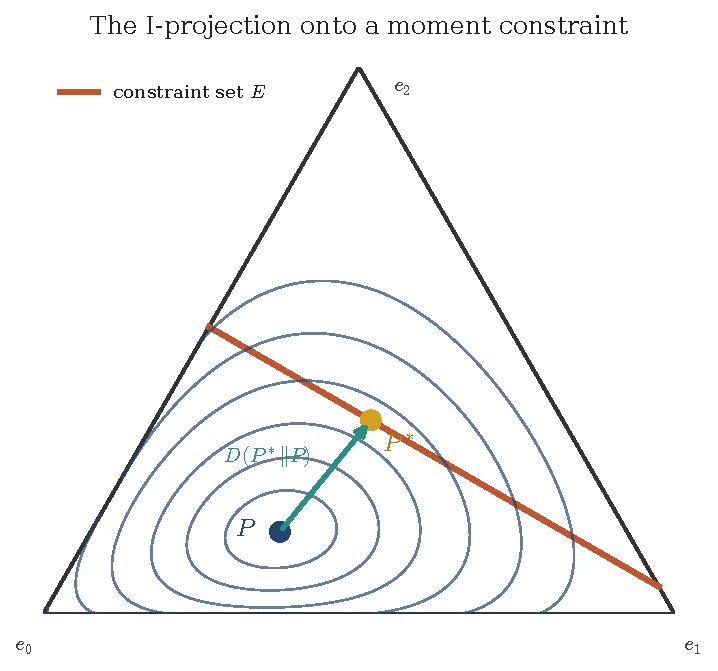
\includegraphics[width=0.72\textwidth]{app_iprojection}
\caption{The I-projection on the simplex of distributions over three outcomes. Contours are level
sets of the divergence from the generating law $P$; the straight line is a moment constraint. The
I-projection $\Pstar$ is the point of the constraint set nearest $P$ in divergence, and
$\D{\Pstar}{P}$ is the Sanov exponent.}
\label{fig:app_iprojection}
\end{figure}

The consequence for this book is the one advertised by the identity de Finetti $+$ Sanov $=$ Bayes (Section~\ref{ch:predictive}). Conditioning an exchangeable sequence
on an empirical constraint is a large deviation event, Sanov says such an event is realized in the
cheapest way available, and the cheapest way is the I-projection of the baseline onto the constraint
set. Bayesian updating under such a constraint therefore does not merely resemble an information
projection, it \emph{is} one, and the posterior inherits the geometry of the divergence rather than
that of the parameter space. Everything from the Gibbs conditioning principle below to
the moderate deviation calibration of later chapters is a refinement of this single exponent.

\subsection{The I-projection and the divergence gap}
For closed convex $E\subseteq\Delta(\X)$ and $P>0$, the I-projection
$\Pstar=\arg\min_{Q\in E}\D{Q}{P}$ is unique by strict convexity; for an affine moment set
$E=\{Q:\langle h,Q\rangle=\alpha\}$ with $\alpha$ in the relative interior of the convex hull of $h(\X)$ it is the exponential tilt $\Pstar(x)\propto P(x)e^{\lambda^\top h(x)}$
with $\lambda$ fixed by $\langle h,\Pstar\rangle=\alpha$; for $\alpha$ on the relative boundary of the hull every $Q\in E$ is carried by the points $x$ with $h(x)$ in the smallest face of the hull containing $\alpha$, and $\Pstar$ is the tilt of $P$ conditioned on those points. The Csisz\'ar Pythagorean inequality,
$\D{Q}{P}\ge\D{Q}{\Pstar}+\D{\Pstar}{P}$ for $Q\in E$, combined with Pinsker's inequality
$\D{Q}{\Pstar}\ge 2\lVert Q-\Pstar\rVert_\TV^2$, gives the divergence-gap bound
\begin{equation}\label{eq:gap}
\D{Q}{P}-\D{\Pstar}{P}\ \ge\ 2\lVert Q-\Pstar\rVert_\TV^2,\qquad Q\in E.
\end{equation}
Inequality \eqref{eq:gap} is the engine of the concentration estimate in Section~\ref{ch:master}: it
converts distance from the projection into an exponential penalty on the type.

\subsection{Sanov by the dominant type}
The theorem has a one-paragraph proof once the type bound is in hand. For the upper bound, sum
\eqref{eq:typebound} over the types in $E$: there are at most $(N+1)^k$ of them, each with
probability at most $e^{-N\D{Q}{P}}\le e^{-N\D{\Pstar}{P}}$, so
$\Pb_P(\Phat_N\in E)\le(N+1)^k e^{-N\D{\Pstar}{P}}$, and the polynomial factor is negligible on
the exponential scale. For the lower bound, keep a single type: pick $Q_N\in E$ on the lattice
with $Q_N\to\Pstar$, so that $\Pb_P(\Phat_N\in E)\ge(N+1)^{-k}e^{-N\D{Q_N}{P}}$, and let
$N\to\infty$. The two bounds meet at $-\D{\Pstar}{P}$. The moral is that a rare empirical event is
carried almost entirely by its cheapest realizable type: the enumeration of types is polynomial and the
divergence is extensive, so one term dominates the sum.

\subsection{Exponential families, maximum entropy, and the tilt}
The $I$-projection wears three hats. As a projection it is $\arg\min_{Q\in E}\D{Q}{P}$; as an
exponential tilt it is $\Pstar(x)\propto P(x)e^{\lambda^\top h(x)}$ for the moment set $\{Q:\langle
h,Q\rangle=\alpha\}$; and as a maximum-entropy law it maximizes $H(Q)$ under the same moment constraint
when $P$ is uniform. These are one object: the exponential family through $P$ with sufficient statistic
$h$, the family the constrained horizon of Section~\ref{ch:master} selects. The multiplier $\lambda$ is
the natural parameter, fixed by matching $\langle h,\Pstar\rangle=\alpha$, and the map
$\lambda\mapsto\alpha$ is the gradient of the log-partition function, monotone by convexity. Every
conjugate Bayesian update, every Gibbs distribution of statistical mechanics, and every maximum-entropy
model is an instance, which is why the tilt recurs in every later chapter as the canonical answer to the
question of what the data force.


\subsection{The conditional limit theorem}
Sanov gives the probability of the constraint; the conditional limit theorem says what the sample
looks like given that the constraint holds.

\begin{theorem}[van Campenhout and Cover; Csisz\'ar]\label{thm:vcc}
For $X_i$ i.i.d.\ $\mu>0$ conditioned on the empirical average of an integer-valued $g$ (along the $N$ for which this event has positive probability, with $\alpha$ in the relative interior of the convex hull of $g(\X)$),
\[
\Pb_\mu\Bigl(X_1=x\ \Bigm|\ \tfrac1N\textstyle\sum_{i=1}^N g(X_i)=\alpha\Bigr)\longrightarrow
\Pstar_\mu(x)=\frac{\mu(x)\,e^{\lambda^\top g(x)}}{\sum_y \mu(y)e^{\lambda^\top g(y)}},
\]
with $\lambda$ fixed by $\langle g,\Pstar_\mu\rangle=\alpha$; any fixed $m$ coordinates are
asymptotically i.i.d.\ $\Pstar_\mu$, the I-projection $\arg\min_{Q\in E}\D{Q}{\mu}$ onto $E=\{Q:\langle g,Q\rangle=\alpha\}$.
\end{theorem}

The conditioned coordinates are not independent at finite $N$, since conditioning on the empirical
measure couples them; independence is recovered only in the limit. Conditioning on a rare event does
not distort a sample arbitrarily. It distorts it in the cheapest way, and \eqref{eq:typebound} says
cheapness is relative entropy. This is the \emph{Gibbs conditioning principle}, and it is the
probabilistic content of the maximum-entropy formalism.

\subsection{Cram\'er's theorem and the Legendre transform}
Sanov's rate is stated over distributions; its one-dimensional shadow is more familiar. For a real
statistic $\bar X_n=n^{-1}\sum_i f(X_i)$, contracting the rate along the map $Q\mapsto\E_Q[f]$ gives
Cram\'er's theorem for $a>\E_P[f]$,
\[
\tfrac1n\log\Pb(\bar X_n\ge a)\to -I(a),\qquad
I(a)=\sup_\lambda\{\lambda a-\log M(\lambda)\},\quad M(\lambda)=\E_P[e^{\lambda f}],
\]
the Legendre transform of the cumulant generating function. The supremum is attained at the tilt
$\lambda^\star$ solving $M'(\lambda)/M(\lambda)=a$, the exponential-family member with mean $a$, so
Cram\'er's minimizer and Sanov's $I$-projection are the same tilted law seen through $f$. The rate
function $I$ is nonnegative and convex and vanishes only at the mean $\E_P[f]$; its curvature there is
the reciprocal variance, $I''(\E_P f)=1/\Var_P(f)$, which seeds the Gaussian behavior near the mean and
the moderate-deviation scale that sits between the center and the Cram\'er zone
(Section~\ref{ch:deviations}).

\subsection{Testing: Stein's lemma and Chernoff information}
The same rates price hypothesis tests. To decide between $P$ and $Q$ from i.i.d.\ data, fixing the
type~I error at a level $\alpha$ and minimizing the type~II error gives, by Stein's lemma, an error
exponent equal to $\D{P}{Q}$: the best rate for the missed alarm is the divergence from the truth to the
alternative. If both errors are driven down together, the Bayes error decays at the Chernoff
information $C(P,Q)=-\min_{0\le s\le1}\log\sum_x P(x)^{s}Q(x)^{1-s}$, the value of the tilted family at
its balancing point. Both are $I$-projection statements: the optimal test compares the empirical type to
the two hypotheses and rejects toward whichever projection is cheaper. This is the information-theoretic
reading of Neyman--Pearson on which the testing and e-value sections build; these exponents are large-deviation rates, whereas the
Bayes-risk threshold of Section~\ref{ch:risk} for a composite alternative lives on the moderate-deviation scale.

\subsection{The three deviation scales}
Sanov and Cram\'er describe the large-deviation zone, where the empirical mean sits a constant away from
its expectation and the rate is the full divergence. Two other scales matter as much for inference. At
the central-limit scale the deviation is $O(n^{-1/2})$ and fluctuations are Gaussian with variance
$1/\{n\,I''(\E_P f)\}$ read from the curvature of the rate function. Between them lies the
\emph{moderate-deviation} scale: for $a_n$ with $1\ll a_n\ll\sqrt n$,
\[
a_n^{-2}\log\Pb\bigl(\bar X_n-\E_P f\ \ge\ a_n\,\sigma/\sqrt n\bigr)\longrightarrow -\tfrac12,
\]
the Gaussian rate function $x^2/2$ \emph{regardless} of the underlying distribution, provided $\sigma^2=\Var_P(f)>0$ and $M(\lambda)<\infty$ near $0$. This universality is
what licenses summary-statistic procedures at thresholds that grow slowly with $n$, and it is the scale
on which Bayes-risk-optimal testing operates, as Section~\ref{ch:risk} shows and
Section~\ref{ch:deviations} proves. The book's recurring $\sqrt{\log n}$ threshold lives permanently in
this middle zone: far enough into the tail that the central limit theorem is useless, not so far that the
answer depends on the whole distribution.

\subsection{Maximum entropy as a modeling principle}
Read forward rather than as a limit theorem, the Gibbs conditioning principle is a modeling
prescription: given only moment information $\E[h]=\alpha$ about a phenomenon, the least committal law
consistent with it is the maximum-entropy tilt $p(x)\propto e^{\lambda^\top h(x)}$. Jaynes made this the
foundation of statistical mechanics and of objective prior construction; here it is a corollary of Sanov,
since the maximum-entropy law is the one the data overwhelmingly realize when nothing beyond the moments
is fixed. The principle is honest about its inputs: choosing which moments to constrain is choosing a
sufficient statistic, and the resulting exponential family is only as good as that choice. What it
guarantees is that, the constraints once fixed, no further structure has been smuggled in, which is
the neutrality the reference-prior program of Section~\ref{ch:risk} demands.



\subsection{Equivalence of ensembles}
The construction has a statistical-mechanics reading that makes the master inequality of
Section~\ref{ch:master} an equivalence-of-ensembles statement rather than a metaphor. Conditioning on
$\{\Phat_N\in E_{\varepsilon_N}\}$ fixes a macroscopic moment window and so defines an
approximately microcanonical ensemble; the product I-projection $(\Pstar_\mu)^{\otimes m}$ is the
canonical law selected by the Lagrange multipliers conjugate to the moment functions. Writing
$\D{Q}{\mu}=-H(Q)-\sum_x Q(x)\log\mu(x)$ exhibits relative entropy as the intensive free-energy cost
of the macrostate $Q$ against the baseline $\mu$, and the I-projection minimizes it. The bad-type
mass in the proof obeys a competition between the combinatorial entropy $2k\log(N+1)$ and the extensive
divergence barrier $2N\delta^2$; balancing them fixes the split radius
$\delta_N\asymp\sqrt{(k\log N)/N}$, not as a free parameter but as the radius at which combinatorial
entropy is offset by divergence cost.



\subsection{Why relative entropy, and not another divergence}
It is fair to ask why relative entropy, rather than some other discrepancy, sets every rate in this
chapter. Three answers converge. Combinatorially, the method of types leaves no choice: the log-probability of
the set of sequences of type $Q$ under $P$ is $-N\D{Q}{P}+o(N)$, so any correct large-deviation rate must be this
divergence. Axiomatically, the Shore--Johnson (1980) theorem shows relative entropy is the unique updating rule
consistent with a few natural requirements, system and subset independence among them, so
maximum-entropy inference is forced once those are accepted. Geometrically, relative entropy is the
canonical divergence of an exponential family, with the Fisher information as its local quadratic form,
which is why its curvature returns as asymptotic variance. Euclidean distance satisfies none of these; it
answers a question about coordinates rather than about probability. Relative entropy is not one
divergence among many but the one the counting, the axioms, and the geometry all select.

\subsection{From Sanov to Bayes: a preview of the synthesis}
The pieces assembled here become the synthesis of the next chapter once the roles of the two arguments of
the divergence are exchanged. Forward, Sanov and the Gibbs conditioning principle say that conditioning a
sample on an empirical constraint tilts it to the $I$-projection
$\Pstar_\mu=\arg\min_Q\D{Q}{\mu}$. Inverted, the same divergence in the other argument,
$\mu\mapsto\D{\Phat_n}{\mu}$, is the posterior energy: the directing law is pulled toward the empirical
distribution at exponential cost, and the posterior is itself a Gibbs measure. De Finetti supplies the
mixture structure, Sanov supplies the tilt, and their composition is Bayesian prediction. This chapter has
built the tilt; Section~\ref{ch:master} builds the composition, and its shape is already visible: a
within-component $I$-projection wrapped in a between-component reweighting, each governed by the one
divergence.


\subsection*{Worked example: the exponential tilt}
Take $P=\mathrm{Exp}(1)$ and the rare event $\{\bar X_n\ge a\}$ for $a>1$, the sample mean exceeding its expectation. The $I$-projection minimizes $\D{Q}{P}$ over laws with $\E_Q[X]=a$; the solution is the exponential tilt $P_\lambda(dx)\propto e^{\lambda x}P(dx)$, which for $P=\mathrm{Exp}(1)$ is again exponential, $P_\lambda=\mathrm{Exp}(1-\lambda)$ with mean $1/(1-\lambda)$. Matching the mean to $a$ fixes $1-\lambda=1/a$, so $\Pstar=\mathrm{Exp}(1/a)$ and
\[
\D{\Pstar}{P}=\int_0^\infty \tfrac1a e^{-x/a}\log\frac{\tfrac1a e^{-x/a}}{e^{-x}}\,dx=a-1-\log a.
\]
Sanov's theorem for a general alphabet (Theorem~\ref{thm:sanov} is stated for a finite alphabet) then yields $\Prob(\bar X_n\ge a)\doteq e^{-n(a-1-\log a)}$, Cram\'er's rate for the exponential recovered as an $I$-projection divergence. For $a=2$ the exponent is $1-\log2\approx0.307$, so the mean of $n=50$ unit exponentials exceeds $2$ with probability $\doteq e^{-15.3}$. The rate alone gives $e^{-50(1-\log2)}=2.2\times10^{-7}$, while the exact tail $\Prob(\bar X_{50}\ge2)=1.2\times10^{-8}$, a $\mathrm{Gamma}(50,1)$ probability, is smaller by a factor of about $18$, the $\Theta(n^{-1/2})$ prefactor that the rate discards, as in the binomial example of Section~\ref{ch:types}. Gibbs conditioning adds the reading: conditioned on the rare event, the sample looks like i.i.d.\ $\mathrm{Exp}(1/a)$ draws, the reference law reshaped to make the once-rare mean typical.

\paragraph{Summary.}
Sanov's theorem states $\Prob(\Phat_n\in E)\doteq e^{-n\inf_{Q\in E}\D{Q}{P}}$: the probability of a rare empirical event decays at the rate of the $I$-projection of $P$ onto $E$. For an affine moment set $E$ the projection is an exponential tilt of $P$ and satisfies a Pythagorean identity (only the inequality for a general convex $E$), and the Gibbs conditioning principle says that conditioned on the rare event the sample looks like i.i.d.\ draws from the projection.

\subsection*{Problems}
\begin{enumerate}[leftmargin=2.2em,itemsep=2pt]
\item For $P>0$ on a finite alphabet and $\min_xf(x)<a<\max_xf(x)$, compute the $I$-projection of $P$ onto the moment set $\{Q:\E_Q[f]=a\}$ and show it is the exponential family\index{exponential family} member $P_\lambda\propto P\,e^{\lambda f}$.
\item Verify the Pythagorean identity $\D{Q}{P}=\D{Q}{\Pstar}+\D{\Pstar}{P}$ for the $I$-projection $\Pstar$ onto an affine set $E$ and any $Q\in E$.
\item Prove the Sanov lower bound by exhibiting a single type in $E$ that dominates.
\item Deduce Cram\'er's theorem for the empirical mean as a one-dimensional corollary of Sanov.
\item State the Gibbs conditioning principle and prove convergence of the one-coordinate conditional law to the tilted measure.
\end{enumerate}

\src{De Finetti + Sanov = Bayes (2509.13283), \S2.3, \S5; Csisz\'ar (1984); van Campenhout and Cover
(1981); L\'eonard and Najim (2002).}

%====================================================================================================

%====================================================================================================

\chapter{The Tilted de Finetti Synthesis}\label{chap:tilted}

The book's central result lives here. De Finetti tells us that an exchangeable sequence is a
mixture of i.i.d.\ laws; Sanov tells us how empirical measures concentrate. Put together, they yield
the tilted de Finetti theorem: conditioning an exchangeable sequence on empirical moment constraints
produces predictive laws obtained by information projection of a baseline measure.

This is the hinge on which the rest of the argument turns, because it \emph{derives} the
exponential-family, maximum-entropy form of Bayesian updating rather than assuming it. The chapter
builds the result in three movements: a master inequality that controls the block law by splitting the
sample space, a projected limit that identifies which predictive laws the data can force, and an
inverse-Sanov statement that exhibits the posterior itself as a Gibbs measure.

Figure~\ref{fig:fourcorner} is the whole construction on one page. The top row is the outer,
Bayesian level: a prior $\Pi$ over directing measures is reweighted by the moment event into the
constraint posterior $\Pi_{N,E}$, whose weak limit is $\Pi_E$ (Theorem~\ref{thm:projected}). The bottom row is the inner level, inside a single component $\mu$:
forward Sanov prices the moment event, and backward Sanov, which is Gibbs conditioning (the conditional step of Section~\ref{ch:inverse}; inverse Sanov is reserved for the posterior), selects the
I-projection $\Pstar_\mu$. The predictive law closes the square as the posterior mixture of
I-projections.

\begin{figure}[t]
\centering
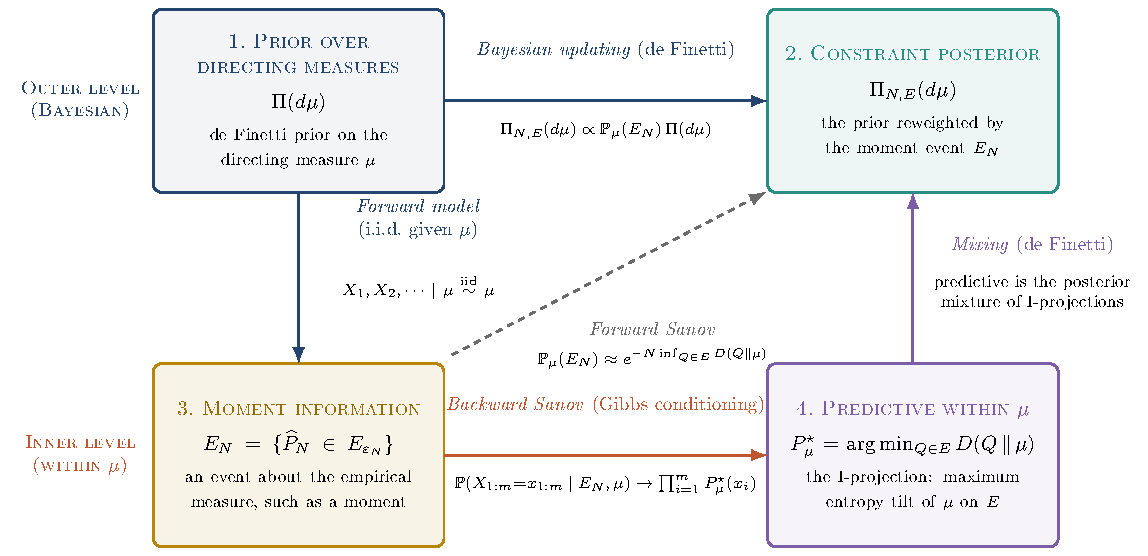
\includegraphics[width=\textwidth]{fig_fourcorner.pdf}
\caption{\small The four corners of the tilted de Finetti theorem. Outer level: the de Finetti
prior over directing measures is updated to the constraint posterior
$\Pi_{N,E}(d\mu)\propto\Pb_\mu(E_N)\,\Pi(d\mu)$ of \eqref{eq:cpost}, whose weak limit is $\Pi_E$ (Theorem~\ref{thm:projected}). Inner level: given $\mu$, forward
Sanov prices the moment event and Gibbs conditioning drives the block law to the product
I-projection. The limiting block law is $\int(\Pstar_\mu)^{\otimes m}\,\Pi_E(d\mu)$: Bayesian at the outer
level, maximum entropy at the inner level.}
\label{fig:fourcorner}
\end{figure}

\paragraph{In what sense ``$=$ Bayes''.} The slogan of the chapter needs an immediate
qualification. De Finetti's theorem already yields the Bayesian scheme from exchangeability alone;
one does not need Sanov's theorem to justify a posterior. The claim here is narrower and
complementary. When the information carried about an exchangeable sequence is a moment constraint
rather than the full sample, the de Finetti predictive update takes a specific and computable form,
the exponential family I-projection, and that form is what Sanov's theorem dictates. Sanov
supplies the shape of the update under partial information; de Finetti supplies its coherence and
the mixing prior. Conditioning on a moment event is an additional and explicit modeling input, not a
consequence of exchangeability, and the chapter flags it wherever it enters.

\paragraph{Two levels: a deterministic tilt and a random directing measure.} Under exchangeability
the directing measure $\mu$ is random with law $\Pi$, and the limit of the one step predictives is
$\mu$ itself, hence random. The results of this chapter are therefore stated at two levels.
Conditionally on $\mu=P$ the sequence is i.i.d.\ $P$, and the constrained block law converges to a
deterministic tilt $\Pstar$ (Theorem~\ref{thm:master}). Released from that conditioning, the limit is
the random measure $\Pstar_\mu$, the I-projection of a random directing measure, whose law is the
push forward of $\Pi_E$ (Theorem~\ref{thm:projected}). Writing ``$X_i$ i.i.d.\ $P$'' inside a theorem
is thus the conditional layer of an exchangeable model, not a departure from it. We keep the
terminology strict: $\Pb(X_{1:m}\in\cdot\mid\cdot)$ is the block, or joint, law, and
``predictive'' is reserved for the law of a future coordinate given the past,
$\Pb(X_{m+1}\in\cdot\mid X_{1:m},\cdot)$. The block law determines the predictive by taking ratios,
so conditionally on $\mu=P$ the one step predictive converges to $\Pstar$ as well, and marginally it
is the posterior mixture of Corollary~\ref{cor:predict}.

\paragraph{What is new and what is not.} The link between maximum entropy and Bayesian inference is
old: it is in Jaynes, in van Campenhout and Cover, in Zabell, and recently in Foley and Scharfenaker
(2025). The emergence of parameters as almost sure limits of predictive functionals is due to
Fortini, Ladelli, and Regazzini (2000; see also Fortini and Petrone, 2012), and moment information has been built directly into
Bayesian nonparametric priors by Bornn, Shephard, and Solgi (2019); the large deviation theory of
exchangeable sequences of Dinwoodie and Zabell (1992) is where the two traditions first meet. What
this chapter adds is a constructive, finite block route from exchangeable observables to
exponential family predictive laws. It names the extra assumption that converts de Finetti into
maximum entropy, namely the moment event; it carries an explicit rate whose constant comes from the
I-projection geometry; and it shows that this rate has the same large deviation geometry as PAC-Bayes
generalization bounds.


\section{The Split-Set Master Inequality}\label{ch:master}

\noindent\textbf{Thesis.} Within a fixed horizon, the constrained block law is close to a product
I-projection, with an explicit finite-$N$ error, uniformly in the location of the block.

\subsection{The constrained-horizon experiment}
We do not begin with a completed unconstrained sample and later observe a rare event. Instead, for
each active horizon $N$, the model is defined by conditioning the exchangeable law on an
empirical-moment restriction. From the de Finetti joint law
$\Pb_N(d\mu,dx_{1:N})=\Pi(d\mu)\,\mu^{\otimes N}(dx_{1:N})$ we impose the primitive constraint
$E_N=\{\Phat_N\in E_{\varepsilon_N}\}$, giving the constrained-horizon law
$\mathbb{Q}_N(d\mu,dx_{1:N})=\Pi_{N,E}(d\mu)\,\mathbb{Q}_{N,\mu}(dx_{1:N})$ with the constraint
posterior
\begin{equation}\label{eq:cpost}
\Pi_{N,E}(d\mu)=\frac{\Pb_\mu(E_N)\,\Pi(d\mu)}{\int \Pb_\nu(E_N)\,\Pi(d\nu)},\qquad
\mathbb{Q}_{N,\mu}(\cdot)=\Pb_\mu(\cdot\mid E_N).
\end{equation}
The restriction is global and permutation invariant; prediction concerns local observables. Because
$\mu^{\otimes N}$ and $E_N$ are permutation invariant, only the cardinality and values of a target
block matter, not its coordinate labels, so a target labeled \emph{future} relative to any finite cut
is subject to the same tilt as any other block inside the horizon.

\subsection{Moment windows and standing assumptions}
Let $g_1,\dots,g_r:\X\to\R$ and thresholds $\alpha_j$ define the polyhedral set
$E=\{Q:\langle g_j,Q\rangle=\alpha_j\ (j\le r_0),\ \langle g_j,Q\rangle\ge\alpha_j\ (r_0<j\le r)\}$
and its window $E_\varepsilon$ by relaxing each bound by $\varepsilon$. We assume: (A1) $k<\infty$;
(A2) $\min_x P(x)>0$; (A3) $E$ nonempty, closed, convex; (A4) the I-projection interior,
$\min_x\Pstar(x)>0$; (A5) strong regularity, $\lVert P^\star_\varepsilon-P^\star_{\varepsilon'}\rVert_\TV\le C_0|\varepsilon-\varepsilon'|$,
which follows from Robinson strong regularity (Robinson, 1980) of the locally active KKT system.

\subsection{The split-set decomposition}
Write $P^\bullet=P^\star_{\varepsilon_N}$ for the window I-projection and split the constrained types
at total-variation radius $\delta$:
\[
\begin{aligned}
G_{N,\delta}&=\{Q\in E_{\varepsilon_N}\cap\mathcal{T}_N:\lVert Q-P^\bullet\rVert_\TV\le\delta\},\\
B_{N,\delta}&=\{Q\in E_{\varepsilon_N}\cap\mathcal{T}_N:\lVert Q-P^\bullet\rVert_\TV>\delta\}.
\end{aligned}
\]
Good types are controlled geometrically by the coupling \eqref{eq:coupling}; bad types are controlled
probabilistically by the divergence gap \eqref{eq:gap}.

\begin{proposition}[Split-set decomposition]\label{prop:split}
Under (A1)--(A5) with $N\varepsilon_N>c_{\mathrm{rnd}}$ eventually, for all large $N$, every
$\delta>0$, and every $m$-element index set $I_N$, with $L_{N,I_N,P}=\mathbb{Q}_{N,P}(X_{I_N}\in\cdot)$ the constrained block law of the component $P$,
\[
\lVert L_{N,I_N,P}-(P^\bullet)^{\otimes m}\rVert_\TV\le m\delta+\frac{m(m-1)}{2N}+\beta_N,\qquad
\beta_N\le C(P,E)(N+1)^{2k}e^{-2N\delta^2}.
\]
\end{proposition}

The constant $c_{\mathrm{rnd}}$ is the rounding constant: rounding a law to a type of $\mathcal{T}_N$ at distance $O(1/N)$ shifts each moment $\langle g_j,\cdot\rangle$ by at most $c_{\mathrm{rnd}}/N$, so $N\varepsilon_N>c_{\mathrm{rnd}}$ leaves a positive margin $\varepsilon_N-c_{\mathrm{rnd}}/N$ and the window $E_{\varepsilon_N}$ contains a type almost as cheap as $P^\bullet$ (Lemma~\ref{lem:denom}), which bounds the normalizing probability from below.

Adding the window-transfer term $\lVert(P^\bullet)^{\otimes m}-(\Pstar)^{\otimes m}\rVert_\TV\le C_0 m\varepsilon_N$
gives the master inequality.

\begin{theorem}[Componentwise constrained-horizon master inequality]\label{thm:master}
Under (A1)--(A5) with $\varepsilon_N\downarrow0$ and $N\varepsilon_N>c_{\mathrm{rnd}}$ eventually,
there is $C(P,E)<\infty$ such that for all large $N$, every $m$-element $I_N$, and every $\delta>0$,
\[
\begin{aligned}
\lVert L_{N,I_N,P}-(\Pstar)^{\otimes m}\rVert_\TV
&\le \underbrace{m\delta+\tfrac{m(m-1)}{2N}}_{\text{good-set approximation}}
+\underbrace{C(P,E)(N+1)^{2k}e^{-2N\delta^2}}_{\text{bad-set mass}}\\
&\quad+\underbrace{C_0\,m\,\varepsilon_N}_{\text{window transfer}}.
\end{aligned}
\]
\end{theorem}


In words, the master inequality says that a fixed block drawn from the constrained horizon is close to
independent draws from the projection $\Pstar$, and it splits the discrepancy into three sources one can
control separately. The good-set term $m\delta+m(m-1)/(2N)$ is the price of approximation inside a small
ball of radius $\delta$ around the projection: the $m\delta$ measures how far a type in the ball can sit
from $\Pstar$, and the $m(m-1)/(2N)$ is the finite-population coupling of Section~\ref{ch:types}, the
chance that an $m$-block drawn with replacement suffers a collision. The bad-set term
$C(N+1)^{2k}e^{-2N\delta^2}$ is the mass on types outside the ball: there are at most $(N+1)^k$ of
them, the lower bound on the normalizing probability costs a further $(N+1)^k$, and each is suppressed by the divergence gap \eqref{eq:gap} at rate $e^{-2N\delta^2}$, so this term
pits an exponential penalty against a polynomial count. The window-transfer term $C_0 m\varepsilon_N$
accounts for the difference between projecting onto the thickened window $E_{\varepsilon_N}$ and onto the
exact constraint. Everything downstream is a matter of choosing $\delta$ to balance the first two.

\begin{corollary}[A tuning]\label{cor:tuning}
Taking $\delta_N=\sqrt{(k+1)\log(N+1)/N}$ gives, for fixed $m$,
\[
\lVert L_{N,I_N,P}-(\Pstar)^{\otimes m}\rVert_\TV
=O\!\left(m\varepsilon_N+m\sqrt{\tfrac{\log N}{N}}+\tfrac{m^2}{N}\right).
\]
\end{corollary}

The tuning makes that balance explicit. The good-set term wants $\delta$ small, while the bad-set term
wants $\delta$ large enough that $e^{-2N\delta^2}$ beats the $(N+1)^{2k}$ polynomial factor; setting the
exponent $2N\delta^2$ equal to $2(k+1)\log(N+1)$, which exceeds the logarithm $2k\log(N+1)$ of that factor by $2\log(N+1)$ and so makes the bad-set term at most $C(P,E)(N+1)^{-2}$, gives $\delta_N=\sqrt{(k+1)\log(N+1)/N}\asymp\sqrt{(k\log N)/N}$, the
radius at which combinatorial entropy is offset by divergence cost. This is the same
entropy-energy balance that fixes the split radius in the thermodynamic reading of
Section~\ref{ch:examples}, and it explains why the final rate carries a $\sqrt{\log N/N}$ rather than the
sharper $1/N$: the logarithm is the bookkeeping cost of the union bound over types, and the $N^{-1/2}$ is
the scale on which the conditioned type fluctuates, which the good-set term pays in full because it charges every type in the ball the distance of the worst one.

The tuned rate has a learning theoretic reading. Its leading term $m\sqrt{(k+1)\log(N+1)/N}$ has
the $\sqrt{\KL/N}$ shape of a PAC-Bayes generalization bound (Catoni, 2007), and the
resemblance is not an accident. Both the contraction of the block law onto the I-projection and PAC-Bayes
risk control are driven by one object, the divergence gap
$\D{Q}{P}-\D{\Pstar}{P}\ge\D{Q}{\Pstar}\ge\tfrac12\lVert Q-\Pstar\rVert_1^2$ for $Q\in E$, which
follows from the Csisz\'ar Pythagorean inequality and Pinsker's inequality; and in both cases the
$\sqrt{\log N}$ is the price of uniform control over a class, here the $(N+1)^k$ types. Because the
gap bound is global rather than a local second order expansion, every constant in
Theorem~\ref{thm:master} can be made explicit. The parallel is structural, not a new bound, and
Section~\ref{ch:evalues} returns to the PAC-Bayes side of it.

The bound is independent of the positions in $I_N$: the constrained component law is exchangeable, so
$I_N=\{1,\dots,m\}$ gives the general case. In the regular exact-sum setting Diaconis and Freedman (1988)
obtain a sharper $O(m/N)$ expansion; the elementary argument trades sharpness for the generality of
polyhedral windows. Only the logarithm in its $\sqrt{\log N/N}$ term is the union-bound artifact over the at most
$(N+1)^k$ types; the $O(m/N)$ comes from averaging the block law over the fluctuations of the type, which cancels their first-order effect, whereas the good-set term bounds each type separately.

\paragraph{Summary.}
The split-set master inequality bounds the distance from the constrained block law to the product I-projection by splitting the constrained types at radius $\delta$ in total variation: the coupling \eqref{eq:coupling} controls the good types, the divergence gap \eqref{eq:gap} controls the bad ones, and the window transfer term $C_0m\varepsilon_N$ accounts for projecting onto the window $E_{\varepsilon_N}$ rather than onto $E$. It is the componentwise half of the tilted de Finetti theorem of this chapter: the inequality turns a large deviation bound on the empirical type into an explicit bound on the block law of each component, and Section~\ref{ch:projected} mixes the components over the constraint posterior.

\subsection*{Problems}
\begin{enumerate}[leftmargin=2.2em,itemsep=2pt]
\item For $k=2$ and $m=2$, compute the total variation distance between $\Pb(X_{1:2}\in\cdot\mid\Phat_N=Q)$, the law of a draw of two items without replacement from $N$ items of which $NQ_1$ are of the first kind, and $Q^{\otimes2}$, and compare it with the coupling bound $m(m-1)/(2N)$ of \eqref{eq:coupling}.
\item Show that $\lVert Q^{\otimes m}-R^{\otimes m}\rVert_\TV\le m\lVert Q-R\rVert_\TV$ for laws $Q,R$ on $\X$. Deduce from \eqref{eq:coupling} that, for $Q\in G_{N,\delta}$, the law $\Pb(X_{1:m}\in\cdot\mid\Phat_N=Q)$ lies within $m\delta+m(m-1)/(2N)$ of $(P^\bullet)^{\otimes m}$ in total variation, and use (A5) with $\varepsilon'=0$ to bound the window-transfer term $\lVert(P^\bullet)^{\otimes m}-(\Pstar)^{\otimes m}\rVert_\TV$ by $C_0m\varepsilon_N$.
\item Let $P>0$, let $E\subseteq\Delta(\X)$ be closed and convex with I-projection $\Pstar$, and let $B=\{Q\in E\cap\mathcal{T}_N:\lVert Q-\Pstar\rVert_\TV>\delta\}$. Using \eqref{eq:typebound} and \eqref{eq:gap}, show that $\Pb_P(\Phat_N\in B)\le(N+1)^ke^{-N\D{\Pstar}{P}}e^{-2N\delta^2}$.
\item Suppose that for some constant $c$ the set $E\cap\mathcal{T}_N$ contains a type $Q_N$ with $\D{Q_N}{P}\le\D{\Pstar}{P}+c/N$. Show that $\Pb_P(\Phat_N\in E)\ge(N+1)^{-k}e^{-c}e^{-N\D{\Pstar}{P}}$ and hence, with $B$ as in the previous problem, $\Pb_P(\Phat_N\in B\mid\Phat_N\in E)\le e^{c}(N+1)^{2k}e^{-2N\delta^2}$. Say which step supplies each of the two factors $(N+1)^k$ in the bad-set term of Theorem~\ref{thm:master}.
\item Show that $\delta_N=\sqrt{(k+1)\log(N+1)/N}$ makes $(N+1)^{2k}e^{-2N\delta_N^2}$ equal to $(N+1)^{-2}$, and that for $\delta_N^2=c\log(N+1)/N$ this quantity tends to $0$ if and only if $c>k$. Conclude that the bad-set term of Theorem~\ref{thm:master} does not tend to $0$ for any radius $\delta_N=o(\sqrt{(\log N)/N})$.
\end{enumerate}

\src{De Finetti + Sanov = Bayes (2509.13283), \S3; Bayesian Prediction under Moment Conditioning
(2510.20742).}

\section{The Projected de Finetti Limit and Reachability}\label{ch:projected}

\noindent\textbf{Thesis.} After mixing over the constraint posterior, the finite-dimensional
marginals converge to an exchangeable law whose random directing measure is the componentwise
I-projection. What survives is a dichotomy between reachable and unreachable constraints.

\subsection{The projected de Finetti limit}
Release the conditioning on $\mu$. Writing $T_E(\mu)=\Pstar_\mu=\arg\min_{Q\in E}\D{Q}{\mu}$ for the
projection map, the exact finite-$N$ identity is
$\mathbb{Q}_N(X_{I_N}\in\cdot)=\int \mathbb{Q}_{N,\mu}(X_{I_N}\in\cdot)\,\Pi_{N,E}(d\mu)$.

\begin{theorem}[Projected de Finetti limit]\label{thm:projected}
Suppose (i) $\Pi_{N,E}\toL\Pi_E$ weakly; (ii) $T_E$ is continuous on a neighborhood of
$\operatorname{supp}(\Pi_E)$; and (iii) for every fixed $m$,
$\int\lVert \mathbb{Q}_{N,\mu}(X_{1:m}\in\cdot)-T_E(\mu)^{\otimes m}\rVert_\TV\,\Pi_{N,E}(d\mu)\to 0$.
Then for every fixed $m$ and every sequence of $m$-element sets $I_N$,
\[
\mathbb{Q}_N(X_{I_N}\in\cdot)\longrightarrow \int T_E(\mu)^{\otimes m}\,\Pi_E(d\mu)
\]
in total variation. With $\widetilde\Pi_E=(T_E)_\#\Pi_E$, the family
$\widetilde{\Pb}^{(m)}_E=\int q^{\otimes m}\,\widetilde\Pi_E(dq)$ is projectively consistent and
defines an infinite exchangeable law $\widetilde{\Pb}_E=\int q^{\otimes\infty}\,\widetilde\Pi_E(dq)$
whose random directing measure is $Q^\star=\Pstar_\mu$, $\mu\sim\Pi_E$.
\end{theorem}

\begin{proof}
By the exchangeability \eqref{eq:cpost} and the triangle inequality, the error splits into the
posterior-averaged component control (iii), which vanishes, and
$\lVert\int T_E(\mu)^{\otimes m}\,\Pi_{N,E}(d\mu)-\int T_E(\mu)^{\otimes m}\,\Pi_E(d\mu)\rVert_\TV$.
The function $f_{x_{1:m}}(\mu)=\prod_{i=1}^m \Pstar_\mu(x_i)$ is bounded by $1$ and continuous on
$\operatorname{supp}(\Pi_E)$ by (ii), so the bounded almost-everywhere-continuous Portmanteau theorem
with (i) gives convergence; summing over the finitely many $x_{1:m}$ gives total variation.
Kolmogorov extension supplies $\widetilde{\Pb}_E$. The architecture is that of
Theorem~\ref{thm:hs}, with the projection inserted: the polynomial $g_s$ is replaced by the tilted
integrand $f_{x_{1:m}}$, Helly--Bray by Portmanteau, and the only new cost is the continuity
requirement on $T_E$, vacuous in the untilted case.
\end{proof}

\begin{corollary}[Bayesian prediction under the constrained limit]\label{cor:predict}
Under $\widetilde{\Pb}_E$, for fixed $t$ and a history $x_{1:t}$ of positive marginal probability,
\[
\widetilde{\Pb}_E(X_{t+1}=x\mid X_{1:t}=x_{1:t})
=\frac{\int \Pstar_\mu(x)\prod_{j=1}^t \Pstar_\mu(x_j)\,\Pi_E(d\mu)}
{\int \prod_{j=1}^t \Pstar_\mu(x_j)\,\Pi_E(d\mu)},
\]
the standard de Finetti posterior predictive under the induced prior
$\widetilde\Pi_E=(T_E)_\#\Pi_E$, with $\widetilde{\Pb}_E(X_{t+1}\in\cdot\mid X_{1:t})\to Q^\star$ a.s.
\end{corollary}

This is the cleanest expression of the identity de Finetti $+$ Sanov $=$ Bayes (Section~\ref{ch:predictive}): Sanov determines the transformed component
$\Pstar_\mu$, de Finetti supplies Bayesian prediction under the resulting law.

\begin{remark}[Fluctuations: a constrained Bernstein--von Mises theorem]\label{rem:cbvm}
The total variation rates describe contraction onto the tilt; the fluctuations around it are
Gaussian. Take $r_0$ linear equality constraints with exact lattice conditioning, so that the window
projection is $\Pstar$ itself. On the $N^{-1/2}$ scale the divergence is quadratic,
$\D{\Pstar+N^{-1/2}h}{\Pstar}=\tfrac1{2N}h^\top\mathcal I(\Pstar)h+O(N^{-3/2})$ with
$\mathcal I(\Pstar)=\diag(1/\Pstar(x))$, and the conditional law of $\sqrt N(\Phat_N-\Pstar)$ given the
constraint is Gaussian on the tangent space $\{h:\sum_xh(x)=0,\ \langle h,g_j\rangle=0\}$ with the
constrained inverse Fisher covariance. Equivalently
\[
2N\,\D{\Phat_N}{\Pstar}\ \toL\ \chi^2_{k-1-r_0},
\]
which is the relative entropy form of Jaynes' entropy concentration theorem: for a uniform baseline, among the sequences that
satisfy the constraint, an overwhelming majority have empirical entropy within $O(1/N)$ of the maximum. A window
can change the limit. If $P$ itself satisfies the constraints, then $P^\bullet=\Pstar=P$, and a window with $\sqrt N\varepsilon_N\to c\in(0,\infty)$ leaves the constrained moments a fluctuation of order $N^{-1/2}$: $2N\,\D{\Phat_N}{P}$ converges in law to $\chi^2_{k-1-r_0}$ plus an independent $V^\top\Sigma_g^{-1}V$, where $\Sigma_g$ is the covariance matrix of $(g_1(X),\dots,g_{r_0}(X))$ for $X\sim P$ and $V\sim\N(0,\Sigma_g)$ is conditioned on $[-c,c]^{r_0}$, and to $\chi^2_{k-1}$ when $\sqrt N\varepsilon_N\to\infty$. The limit comes from splitting the Pearson statistic $N\sum_x(\Phat_N(x)-P(x))^2/P(x)$, to which $2N\,\D{\Phat_N}{P}$ is asymptotically equal, into $V_N^\top\Sigma_g^{-1}V_N$ with $V_N=\sqrt N(\langle g_j,\Phat_N\rangle-\alpha_j)_{j\le r_0}\toL\N(0,\Sigma_g)$ and a remainder that is asymptotically $\chi^2_{k-1-r_0}$ and independent of $V_N$: the window event $\{\Phat_N\in E_{\varepsilon_N}\}=\{\max_j\lvert V_{N,j}\rvert\le\sqrt N\varepsilon_N\}$ conditions $V_N$ alone. For a general window, Section~\ref{ch:examples} explains why a two-scale local limit theorem is needed and leaves that case open. For the
Brandeis die ($k=6$, one constraint, mean $4.5$) a simulation that conditions multinomial samples on
the exact sum gives $2N\,\D{\Phat_N}{\Pstar}$ mean $4.06$ and variance $8.31$ at $N=200$ ($37{,}110$ accepted samples), and mean
$4.00$ and variance $8.00$ at $N=1000$ ($16{,}731$ accepted samples), against $4$ and $8$ for $\chi^2_4$, with Kolmogorov distance
$0.006$ at $N=1000$. The deterministic tilt $\D{\Pstar}{P}$, the Gaussian fluctuation
$\D{\Phat_N}{\Pstar}$, and the de Finetti update $\Pi\to\Pi_E$ are the three layers of the
construction.
\end{remark}

\subsection{Reachability and degeneracy}
The constraint posterior is exponentially weighted: pointwise in $\mu$,
$\frac1N\log\Pb_\mu(E_N)\to-I_E(\mu)$ with $I_E(\mu)=\inf_{Q\in E}\D{Q}{\mu}$, so
$\Pi_{N,E}(d\mu)\propto e^{-N I_E(\mu)+o_\mu(N)}\Pi(d\mu)$.

\begin{proposition}[Reachability and degeneracy]\label{prop:reach}
Since $\D{Q}{\mu}=0$ only at $Q=\mu$, $I_E$ vanishes exactly on $E$.
\begin{enumerate}[label=(\roman*),leftmargin=2em]
\item \emph{Reachable, positive mass.} If $\Pi(E)>0$ and $\Pi(\partial E)=0$, with $\partial E$ the boundary of $E$ in $\Delta(\X)$, then $\Pi_E=\Pi(\cdot\mid E)$ and $T_E$ is the
identity on $E$: the constraint truncates the prior and the I-projection is asymptotically inactive. The boundary condition is needed: a window of order $N^{-1/2}$ can accept a component on $\partial E$ with limiting probability below $1$, and atoms of $\Pi$ there are then reweighted.
\item \emph{Reachable, null.} If $\Pi(E)=0$ but $E\cap\operatorname{supp}\Pi\ne\emptyset$, then
$\Pi_{N,E}$ concentrates on $E$ at rate $\max(\varepsilon_N,N^{-1/2})$ and $\Pi_E$ is the disintegration of $\Pi$ along
the moment map at $\alpha$; again $T_E|_E=\mathrm{id}$.
\item \emph{Unreachable.} If $I^\star=\inf_{\operatorname{supp}\Pi}I_E>0$ then $\Pi_{N,E}$
concentrates on $\{I_E=I^\star\}$ and the surviving components are genuine tilts.
\item \emph{Degeneracy.} For affine $E$ with $r_0$ equalities, $\Pstar_\mu=\Pstar_\nu$ iff $\mu,\nu$
lie in a common orbit of the exponential family generated by $g_1,\dots,g_{r_0}$; the surviving
randomness is the component of $\Pi_E$ transverse to the tilt family, of dimension $k-1-r_0$.
\end{enumerate}
\end{proposition}

We state the proposition without proof: clauses (i) to (iii) follow from the exponential weighting of $\Pi_{N,E}$ above by Laplace's method, and (iv) holds because each $\Pstar_\mu$ is an exponential tilt of $\mu$ by $g_1,\dots,g_{r_0}$. Clause (ii) is the default: an equality constraint makes $E$ a lower-dimensional slice, so any prior
with a density gives $\Pi(E)=0$ while $I_E$ still vanishes on $E$. It carries a warning, the
Borel--Kolmogorov paradox: because $\Pi(E)=0$, the symbol $\Pi(\cdot\mid E)$ is undefined without
nominating an approximating family. The entropy tube $\{\Phat_N\in E_{\varepsilon_N}\}$ nominates one,
the disintegration along the moment map, and it is that conditional, and no other, which appears in
the limit.

\begin{example}[The null-constraint trap]
Take $\X=\{1,2,3\}$, $g(x)=x$, $E=\{Q:\E_Q[X]=2.2\}$, and the flat prior
$\Pi=\mathrm{Dir}(1,1,1)$, so $\Pi(E)=0$ while $I_E$ vanishes on $E$. The co-area disintegration
predicts $\E[\mu_3\mid E]=0.4$ exactly, whereas Laplace's method applied to the large-deviation form
alone predicts the $\sigma$-reweighted law $\Pi_E\propto\sigma(\mu)\Pi$, with $\sigma^2(\mu)=\Var_\mu(X)$, giving $0.4255$: a $2.6$
percentage-point error in a predictive probability. The exact finite-$N$ constraint posterior
converges to $0.400$ from below at rate $O(1/N)$, excluding the reweighting. A large-deviation rate
identifies where the posterior concentrates; it does not by itself identify the conditional it
concentrates to. The polynomial prefactor, which \eqref{eq:typebound} only brackets between $(N+1)^{-k}$ and $1$, is supplied by the local limit theorem; it carries the
factor $\det\Omega^{-1/2}$, with $\Omega=\Cov_\mu(g(X))$ the covariance of the constraint statistic ($\Omega=\sigma^2(\mu)$ here), and this factor cancels the Gaussian tube Jacobian.
\end{example}

\begin{example}[Location-free Bernoulli and Brandeis dice]
With $\mu=\mathrm{Ber}(0.2)$ and the horizon mean constrained near $0.8$, the I-projection is
$\mathrm{Ber}(0.8)$ and every fixed target inside the horizon is asymptotically $\mathrm{Ber}(0.8)$,
regardless of its temporal label; the equality constraint is affine with $k-1-r_0=0$, so
Proposition~\ref{prop:reach}(iv) forces a degenerate directing measure and no prior survives. The
Brandeis dice of Section~\ref{ch:predictive} is the maximum-entropy instance with a uniform baseline;
under uncertain die laws the induced prior $\widetilde\Pi_E$ governs the Bayesian mixture. Under
Gaussian scale mixtures, mean-only conditioning leaves the variance transverse to the tilt and the
limit is nondegenerate, while mean-and-variance conditioning exhausts the transverse direction and
the mixture collapses.
\end{example}

\paragraph{Summary.}
Under moment constraints the de Finetti mixing measure of the large-sample limit, $\widetilde\Pi_E=(T_E)_\#\Pi_E$, lives on the constraint set, and reachability decides whether the projection acts. When $E$ meets the support of the prior, the constraint posterior $\Pi_{N,E}$ concentrates on $E$ and the projection is the identity there; when it does not, $\Pi_{N,E}$ concentrates on $\{I_E=I^\star\}$, off $E$, and the surviving components are genuine tilts. Either way a limiting directing law is the I-projection $\Pstar_\mu$ of a law $\mu$ in the support of the prior. This is the constructive content of the synthesis: it says which limits the data can force.

\subsection*{Problems}
\begin{enumerate}[leftmargin=2.2em,itemsep=2pt]
\item Characterize the reachable set for a single linear moment constraint.
\item Show that the projected limit need not be the $I$-projection of the prior predictive onto the constraint set.
\item Give an example where the constraint set is nonconvex and the projection is non-unique.
\item Relate reachability to the existence of a maximum-entropy distribution with the prescribed moments.
\item Prove continuity of the projected limit in the constraint level $a$ where the projection is unique.
\end{enumerate}

\src{De Finetti + Sanov = Bayes (2509.13283), \S4, \S6.}

\section{Inverse Sanov and the Posterior as a Gibbs Measure}\label{ch:inverse}

\noindent\textbf{Thesis.} One divergence organizes the sampling law, the conditioning, and the
posterior. Read forward it is the cost of a type; read inverse it is the energy of a Gibbs measure
over directing laws, and its curvature is the Fisher information\index{Fisher information}.

\subsection{Forward and inverse relative entropy}
On a finite alphabet the full-data likelihood factors through the empirical measure,
\begin{equation}\label{eq:aep}
\mu^{\otimes N}(x_{1:N})=\exp\{-N H(\Phat_N)-N\D{\Phat_N}{\mu}\},
\end{equation}
the exact finite-$N$ form of the asymptotic equipartition property. The entropy term is free of
$\mu$ and cancels in Bayes' rule, leaving the posterior as a Gibbs measure.

\begin{proposition}[Inverse-Sanov representation of the posterior]\label{prop:invsanov}
On a finite alphabet, the de Finetti posterior over the directing measure is
\[
\Pi(d\mu\mid x_{1:N})\ \propto\ e^{-N\D{\Phat_N}{\mu}}\,\Pi(d\mu),
\]
a Gibbs measure at inverse temperature $N$ with energy $\mu\mapsto\D{\Phat_N}{\mu}$.
\end{proposition}

The identity is classical; the content is the joint reading of \emph{one} divergence in three roles.
Forward, $\D{Q}{\mu}$ is the cost of the type $Q$ given $\mu$ (Sanov, Theorem~\ref{thm:sanov}).
Conditional, the moment event selects $\Pstar_\mu$ by Gibbs conditioning (Theorem~\ref{thm:vcc}).
Inverse, $\D{\Phat_N}{\mu}$ is the cost of the directing measure given the data, the energy of
Proposition~\ref{prop:invsanov}; under event conditioning the effective energy is instead $I_E(\mu)$
(Proposition~\ref{prop:reach}). We use ``inverse Sanov'' for this posterior Gibbs geometry, not as a
claim that reversing the arguments always yields a posterior large-deviation principle.

\subsection{The Ganesh--O'Connell theorem and the rate function}
The posterior large-deviation principle is due to Ganesh and O'Connell.

\begin{theorem}[Ganesh and O'Connell, inverse Sanov]\label{thm:go}
For a finite alphabet and a prior charging every nonempty open subset of the simplex, the posterior sequence
$\Pi(\cdot\mid X_{1:N})$ for i.i.d.\ data from $p_0$ satisfies, almost surely, a large-deviation principle at speed $N$ with rate function $J(p)=\D{p_0}{p}$, minimized and
zero at $p=p_0$, and independent of the prior.
\end{theorem}

Sanov rates the empirical measure deviating under the truth by $\D{\Phat_N}{p_0}$; inverse Sanov rates
the posterior mass on a candidate law $p$ by $\D{p_0}{p}$, the same divergence with arguments
reversed. Ganesh and O'Connell (2000) establish the companion large-deviation principle for
Dirichlet posteriors, the setting in which the theorem is most transparent, since the posterior is
$\mathrm{Dir}(\alpha+N\Phat_N)$ and concentrates at the empirical law with rate $\D{p_0}{p}$ and Hessian
$\operatorname{diag}(1/p_{0,i})$ on the simplex tangent space. Macci and Piccioni prove the posterior principle for
subfamilies of exponential families, with rate $\D{p_{\theta_0}}{p_\theta}$ when the model is correct, but show that the maximum likelihood rate is in general not the forward divergence $\D{p_\theta}{p_{\theta_0}}$,
so the reversal of arguments is not an automatic corollary of a Sanov principle for the estimator.

\subsection{The curvature identity and the posterior ladder}
The three asymptotic descriptions of the posterior are one object at three scales, welded by a
single computation.

\begin{proposition}[Curvature identity and its symmetry]\label{prop:curv}
Let $q$ be interior to the simplex and $\sum_i v_i=0$. Both orderings of relative entropy have the
same second-order expansion,
\[
\begin{gathered}
\D{q+\varepsilon v}{q}\ \text{and}\ \D{q}{q+\varepsilon v}\ \text{both equal}\\
\frac{\varepsilon^2}{2}\sum_i\frac{v_i^2}{q_i}+O(\varepsilon^3)
=\frac{\varepsilon^2}{2}\,v^\top\Info(q)\,v+O(\varepsilon^3),
\end{gathered}
\]
with $\Info(q)=\operatorname{diag}(1/q_i)$. In particular $\nabla^2 J|_{p_0}=\Info(p_0)$ for $J(p)=\D{p_0}{p}$.
\end{proposition}

The Fisher information is thus the curvature of the inverse-Sanov rate at the truth, and
Bernstein\index{Bernstein--von Mises theorem}--von Mises is that curvature exponentiated:
\[
\begin{gathered}
\underbrace{\text{Bernstein--von Mises}}_{\text{CLT scale}}\ \longleftrightarrow\
\underbrace{\text{Eichelsbacher--Ganesh}}_{\text{moderate scale}}\ \longleftrightarrow\
\underbrace{\text{inverse Sanov}}_{\text{large scale}},\\
\Info=\nabla^2 J|_{p_0}.
\end{gathered}
\]
The moderate-deviation\index{moderate deviations} principle is the Taylor quadratic of $J$; the central-limit Gaussian is the
exponential of that quadratic. A corollary of Proposition~\ref{prop:curv} is that Bernstein--von
Mises is \emph{blind to the direction} of the divergence: no second-order analysis of the posterior
can distinguish $\D{p_0}{\cdot}$ from $\D{\cdot}{p_0}$, and the asymmetry of Kullback\index{Kullback--Leibler divergence}--Leibler, and
hence the distinction between the Sanov and inverse-Sanov rates, appears only at the large-deviation
scale. This is the organizing lens of Chapter~\ref{chap:asymptotics}: the posterior is Gaussian when $J$ is a
single fixed nondegenerate paraboloid, and every failure of Bernstein--von Mises is a degeneracy of
that curvature.

\subsection{Two local Gaussian phenomena}
The same local quadratic expansion produces two Gaussian statements in opposite arguments of the
divergence. \emph{Forward} conditional Sanov gives Gaussian fluctuations of the empirical type around
the I-projection on the constraint tangent space, with $2N\D{\Phat_N}{\Pstar}$ approaching a
chi-square with $k-1-r_0$ degrees of freedom. \emph{Inverse} Sanov gives Gaussian posterior
fluctuations of the directing law around the empirical distribution: for an interior truth $\mu_0$
and a prior density positive and continuous at $\mu_0$, the finite-dimensional Bernstein--von Mises
theorem gives $\sqrt N(\mu-\Phat_N)\mid X_{1:N}\toL \mathcal N_{k-1}(0,\Info(\mu_0)^{-1})$, where $\Info(\mu_0)^{-1}$ is taken on the tangent space $\{v:\sum_iv_i=0\}$ and equals $\diag(\mu_0)-\mu_0\mu_0^\top$. The
empirical type fluctuates around the projected law; the posterior directing law fluctuates around the
empirical type. Both are the same paraboloid read in opposite arguments.
\subsection{The support condition and the asymmetry of the divergence}
The hypothesis in Theorem~\ref{thm:go} that is easiest to overlook is that the prior charges every nonempty open set, not only neighborhoods of the truth: the posterior puts no mass where the prior puts none, so for a prior supported on a proper closed subset of the simplex that contains the truth the rate is the divergence from the truth on that subset and $+\infty$ off it, and ``independent of the prior'' fails. A support condition on the candidates, by contrast, needs no assumption. Writing $\mu_0$ for the
truth and $\nu$ for the candidates carried by the prior, a candidate with
$\nu(x)=0<\mu_0(x)$ gives probability zero to every sample containing $x$, so the posterior drops it as soon as $x$ is observed; once every point of the truth's support has been observed, the posterior charges only candidates with $\nu(x)=0\Rightarrow\mu_0(x)=0$. The reason, in rate terms, is the asymmetry of relative
entropy.

Sanov rates a candidate by $\D{\nu}{\mu_0}$; inverse Sanov rates it by $\D{\mu_0}{\nu}$. By
Proposition~\ref{prop:curv} the two share a Hessian at $\nu=\mu_0$, so no local analysis can tell them
apart. Globally they penalize very differently. The inverse ordering $\D{\mu_0}{\nu}$ is
\emph{zero-avoiding}: it diverges as soon as $\nu$ puts zero mass anywhere $\mu_0$ puts positive mass, so a
candidate that merely omits part of the truth's support is infinitely costly, whereas under the
forward ordering it is not. That is the behavior a posterior should have, and it is why the
support condition needs no separate assumption. It is also a second reason, beyond the
Macci--Piccioni caution noted above, why the inverse-Sanov ordering must be proved rather than read off the forward one (Theorem~\ref{thm:go} proves it for a finite alphabet) and stays a hypothesis to verify outside the settings where it is proved:
the two divergences agree to second order and diverge in the tails, which is where the
large-deviation statement lives.

\subsection{Which deviation scale makes the Fisher information exact}
Proposition~\ref{prop:curv} gives a quadratic approximation, and the ladder above suggests reading
the middle rung as ``the rate is the Fisher information when $\nu$ is close to $\mu_0$.'' That
statement is true but imprecise, and the imprecision matters for the calibration results of
Section~\ref{ch:deviations}.

The quadratic is \emph{exact}, not merely leading-order, at the moderate-deviation scale:
perturbations of order $a_N/\sqrt N$ with $a_N\to\infty$ and $a_N/\sqrt N\to0$. On that scale, with $\nu=\mu_0+(a_N/\sqrt N)h$, the terms of $N\D{\mu_0}{\nu}$ beyond the quadratic are $o(a_N^2)$, and the
rate function is $\tfrac12 h^\top\Info(\mu_0)h$. At the full large-deviation scale, where
deviations are $O(1)$, no quadratic will do and one needs the complete $\D{\mu_0}{\nu}$. The three
rungs of the ladder are therefore not three approximations of decreasing quality; they are one
function read at three magnifications, and the central-limit and moderate rungs both replace the divergence by
its Hessian, the first as the exponent of a limit law, the Gaussian, and the second as the rate function of probabilities that vanish. This is the analytic content behind the recurring finding that Bayes-risk optimal
calibration lives on the scale $n\lambda_n^2\asymp\log n$, with $\lambda_n=|\hat\theta-\theta_0|$ the deviation of the estimate from the null value, rather than on the central-limit or
large-deviation scales.

In the nonparametric direction the same expansion has a geometric name. For a perturbation
$\nu=\mu_0+\varepsilon h$ with $\int h=0$,
\[
\D{\mu_0}{\nu}\ \approx\ \frac{\varepsilon^2}{2}\int\frac{h(x)^2}{\mu_0(x)}\,dx,
\]
the Fisher--Rao metric (Kass and Vos, 1997), which by Chentsov's theorem (1982) is, up to scale, the unique Riemannian metric on the space of
distributions invariant under sufficient statistics. Proposition~\ref{prop:curv} is its finite-alphabet
instance, with $\Info(q)=\operatorname{diag}(1/q_i)$.

\subsection{Exponential families, where the curvature is global}
On an exponential family the local statement becomes global, which is the cleanest case in the book
and the one Section~\ref{ch:maxent} computes with. For $p_\theta$ in an exponential family with
log-partition\index{log-partition function} $A(\theta)$, the divergence $\D{p_{\theta_0}}{p_\theta}$ equals the Bregman divergence
of $A$, and $\Info(\theta_0)=\nabla^2 A(\theta_0)$. The Fisher information is therefore the Hessian of
the rate function \emph{everywhere} in the natural parameterization, not only at the truth: the Hessian at $\theta$ is $\nabla^2A(\theta)=\Info(\theta)$. The rate is the
paraboloid of Bernstein--von Mises only when $A$ is quadratic, as for a Gaussian location family; otherwise $\Info(\theta)$ varies with $\theta$. What is exact for every exponential family is the Gibbs form of the conjugate posterior: for $p_\theta(x)\propto e^{\theta^\top T(x)-A(\theta)}$ and a proper conjugate prior density $\propto e^{\theta^\top\tau-n_0A(\theta)}$, the posterior density after $x_{1:N}$ is $\propto e^{-(n_0+N)\D{p_{\bar\theta}}{p_\theta}}$ with $\nabla A(\bar\theta)=(\tau+\sum_{i=1}^NT(x_i))/(n_0+N)$, which is why the conjugate gallery closes in
closed form.

\subsection{The rate function as an evidence growth rate}
The inverse-Sanov rate has a second reading that connects this section to the evidence theory of
Section~\ref{ch:evalues}. Let $\mu_0$ be the truth. The Bayes factor\index{Bayes factor} for $\mu_0$ against a candidate $\nu$ is
$\prod_{i=1}^N\mu_0(X_i)/\nu(X_i)$, which under $\mu_0$ grows at
exponential rate $\D{\mu_0}{\nu}$ by the law of large numbers, the rate at which Theorem~\ref{thm:go} makes the posterior mass near $\nu$ decay. The log-optimal e-value\index{e-values} for testing the null $\nu$ against the alternative $\mu_0$ in a
sequential experiment is the Neyman--Pearson likelihood ratio\index{likelihood ratio}, this same product, and its growth rate under $\mu_0$ is the same
$\D{\mu_0}{\nu}$. Evidence accumulates at the inverse-Sanov rate, and the expected time for the likelihood ratio to cross a
boundary $1/\alpha$ is $\log(1/\alpha)/\D{\mu_0}{\nu}$ to first order as $\alpha\to0$. The two objects introduced in this section,
the e-process\index{e-processes} and the posterior, are governed by one function; the difference is whether one reads
it as a rate of accumulation or as a rate of contraction.


\paragraph{Summary.}
Inverse Sanov turns the forward large-deviation statement around: the posterior over the directing measure obeys a large-deviation principle with rate $\D{p_0}{\cdot}$, where $p_0$ is the true directing law (Theorem~\ref{thm:go}), and at every sample size the posterior is a Gibbs measure with energy $\D{\Phat_n}{\cdot}$, minimized at the empirical distribution (Proposition~\ref{prop:invsanov}). This is the sense in which Bayesian updating is reverse $I$-projection, and it is the bridge from the information-theoretic engine to the posterior asymptotics of Section~\ref{ch:asymptotics}.

\subsection*{Problems}
\begin{enumerate}[leftmargin=2.2em,itemsep=2pt]
\item Show that the posterior density is proportional to $e^{-n\D{\Phat_n}{Q}}$ times the prior, to leading exponential order.
\item Deduce posterior consistency\index{posterior consistency}: the posterior concentrates at the true directing measure at rate governed by $\D{\cdot}{\cdot}$.
\item Identify the posterior's Gibbs (exponential-family) form and its natural parameter.
\item Contrast the inverse-Sanov rate with the forward Sanov rate and explain the role reversal of the two arguments of the divergence.
\item Use the result to recover the Bernstein--von Mises Gaussian approximation in the regular case.
\end{enumerate}

\src{De Finetti + Sanov = Bayes (2509.13283), \S4.4; When Is Bayes Gaussian? (2026e); Ganesh and
O'Connell (1998, 1999, 2000); Macci and Piccioni (2023); Fu and Kass
(1988); A New Look at Bayesian Testing (2602.11132).}

%====================================================================================================

%====================================================================================================

\shorthead{Diaconis: Finite de Finetti and Conjugacy}
\section{Diaconis's Program: Finite de Finetti, Conditional Limits, and Conjugate Priors}\label{ch:diaconis}\index{Diaconis}\index{conjugate prior}\index{finite de Finetti theorem}

\noindent\textbf{Thesis.} Persi Diaconis, mostly with David Freedman, worked on almost every theme of
this part of the book, and his results supply three missing pieces. A statistician never has an
infinite exchangeable sequence, and the finite de Finetti theorem says how much of the
representation survives with $n$ observations. The conditional limit theorem for exponential families
says that de Finetti and Sanov are one result seen from two sides. And the Diaconis and Ylvisaker
characterization of conjugate priors says that conjugacy is a statement about prediction, not an
algebraic convenience, with an exact relative entropy form that is the inverse Sanov Gibbs measure of
Section~\ref{ch:inverse} built from an imaginary sample. This section states each result, checks the
numbers, and closes with applied examples from sport and from coin tossing.

\subsection{de Finetti, finitely}\label{dia:sec:finite}

The infinite theorem fails for finite sequences, and the obstruction is visible at $n=2$. Let
$(X_1,X_2)$ be uniform on $\{(0,1),(1,0)\}$. The law is exchangeable, but every mixture of i.i.d.\
Bernoulli laws gives
$\Pb(X_1=X_2)=\int\{p^2+(1-p)^2\}\,\Pi(dp)\ge\tfrac12$, while here the probability is zero. Diaconis
(1977) described the set of finite exchangeable laws that are not mixtures and showed that it shrinks
as the sequence is extended. Diaconis and Freedman (1980a) made the shrinkage quantitative.

\begin{theorem}[Diaconis and Freedman, finite de Finetti]\label{dia:thm:finite}
Let $X_1,\dots,X_n$ be exchangeable with values in $S$, let $P_k$ be the law of $(X_1,\dots,X_k)$, and
let $P_{\Pi,k}$ be the mixture of i.i.d.\ laws directed by the law $\Pi$ of the empirical measure of
$X_1,\dots,X_n$. Then the variation distance between $P_k$ and $P_{\Pi,k}$ is at most $ck/n$ when $S$
has $c$ elements, and at most $k(k-1)/(2n)$ for general $S$. Here variation distance is $\lVert\cdot\rVert_\TV=\sup_A|P(A)-Q(A)|$; Diaconis and Freedman use twice this norm and state the bounds as $2ck/n$ and $k(k-1)/n$.
\end{theorem}

The proof is the urn argument of Theorem~\ref{thm:dfhs1}: given the empirical measure, the first $k$
coordinates are draws without replacement from the $n$ observed values, and the mixture is the same
draws with replacement. The general bound is the birthday computation, which in the sup over events
gives $k(k-1)/(2n)$ as in \eqref{eq:urncoupling}. With finitely many values one can do better than the
birthday bound, because repeated labels only matter through the counts, and the distance becomes
linear in $k/n$.

Figure~\ref{fig:dia_finite} shows the exact distance for an urn of $n$ balls, half marked one. The
first $k$ draws are exchangeable with a point mass mixing measure at one half, and the distance
between the hypergeometric and binomial count laws is close to $k/(4n)$: for $n=1000$ it is $0.0025$,
$0.0125$ and $0.0254$ at $k=10$, $50$ and $100$. The finite state bound $ck/n$ is linear and
conservative; the birthday bound is quadratic and useless once $k$ is of order $\sqrt n$. Gavalakis,
Johnson and Kontoyiannis (2024) start from the same sampling argument and give finite de Finetti
bounds in relative entropy, the natural form for this book; Pinsker's inequality recovers variation
bounds from them.

\begin{figure}[H]
\centering
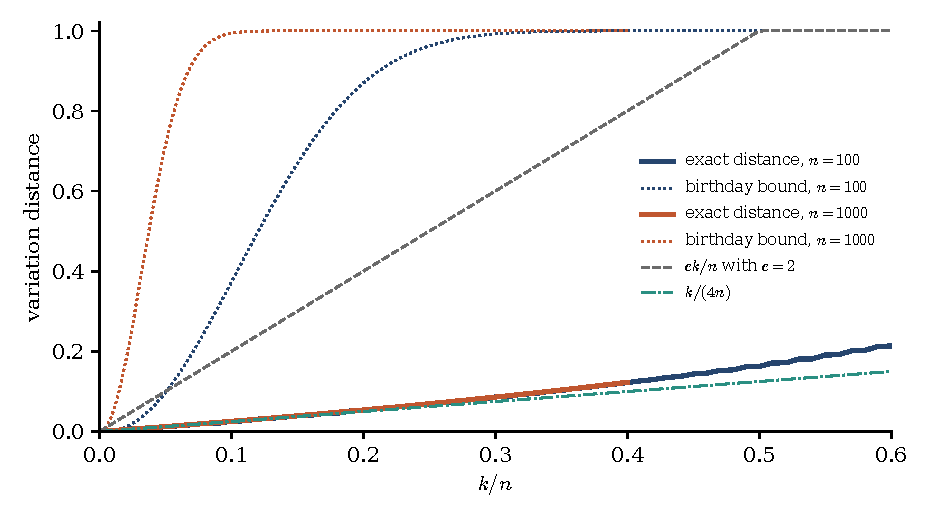
\includegraphics[width=0.8\textwidth]{dia_finite_definetti}
\caption{Finite de Finetti for an urn of $n$ balls, half marked one. Solid: exact variation distance
between the law of the first $k$ draws and the i.i.d.\ mixture. Dotted: the birthday bound. Dashed:
the finite state bound $ck/n$ with $c=2$. Dash dot: $k/(4n)$.}
\label{fig:dia_finite}
\end{figure}

Two extensions matter for later chapters. De Finetti's theorem for Markov chains (Diaconis and
Freedman, 1980b) replaces exchangeability by partial exchangeability, invariance under permutations
that preserve transition counts, and yields mixtures of Markov chains; it is the representation behind
the Markov posterior of Section~\ref{ch:asymptotics}. And their survey of de Finetti style results
(1987) collects characterizations such as that of orthogonally invariant sequences as scale mixtures
of normals, the representation on which the global local shrinkage priors of
Section~\ref{ch:shrinkpics} are built.

\subsection{Sanov from the Bayesian side}\label{dia:sec:sanov}

The deepest link between this program and the information theory of the book is Diaconis and
Freedman (1988). Let $X_1,X_2,\dots$ be i.i.d.\ from a regular exponential family $P_\theta$ with
sufficient statistic $T$, and $S_n=\sum_{i\le n}T(X_i)$.

\begin{theorem}[Diaconis and Freedman, conditional limit, informal]\label{dia:thm:clt}
Under the regularity conditions of Diaconis and Freedman (1988), and for $s$ in the interior of the mean space of $T$, conditionally on $S_n=ns$ the law of $(X_1,\dots,X_k)$ is within variation distance of order $k/n$ of
the i.i.d.\ law $P_{\theta(s)}^{\otimes k}$, where $\theta(s)$ is the parameter at which the mean of $T$
equals $s$. Consequently an exchangeable law whose finite sections share this conditional structure
is, for $k$ small relative to $n$, close to a mixture of the $P_\theta^{\otimes k}$.
\end{theorem}

Read forward, this is the conditional limit theorem of Theorem~\ref{thm:vcc}: conditioning on an
empirical mean selects the exponential tilt, the I-projection of the base law onto the constraint,
which Csisz\'ar (1984) proved through Sanov's theorem with a constraint. Read backward, it is a de
Finetti theorem in which sufficiency forces the mixing family to be an exponential family. The pairing
of de Finetti and Sanov that organizes this book is therefore not a juxtaposition of two topics but a
single result looked at from two sides, and this is the reference that says so; the tilted de Finetti
theorem of Section~\ref{ch:projected} is its random measure version.

\subsection{Conjugate priors as a statement about prediction}\label{dia:sec:conj}

Let $X$ have a natural exponential family density with respect to a measure $\nu$ on $\R^d$,
\[
p(x\mid\theta)=\exp\{\theta^\top x-M(\theta)\},\qquad\theta\in\Theta,
\]
with mean $m(\theta)=\nabla M(\theta)$, a bijection from $\Theta$ onto the interior $\mathcal X^\circ$
of the convex hull of the support of $\nu$. The Diaconis and Ylvisaker prior with prior sample size
$n_0>0$ and prior guess $x_0\in\mathcal X^\circ$ is
\[
\pi(\theta\mid n_0,x_0)=K(n_0,x_0)\exp\{n_0x_0^\top\theta-n_0M(\theta)\},
\]
proper exactly when $n_0>0$ and $x_0\in\mathcal X^\circ$. After $x_1,\dots,x_n$ with mean $\bar x$ the
posterior has the same form with $n_0\mapsto n_0+n$ and $x_0\mapsto x_n=(n_0x_0+n\bar x)/(n_0+n)$:
updating is pooling in the mean space.

\begin{theorem}[Diaconis and Ylvisaker, 1979]\label{dia:thm:dy}
(i) Under the conjugate prior $\E[m(\theta)]=x_0$, and hence
\[
\E[X_{n+1}\mid x_{1:n}]=\E[m(\theta)\mid x_{1:n}]=\frac{n_0x_0+n\bar x}{n_0+n}.
\]
(ii) Conversely, if $\mathcal X^\circ$ is nonempty, the prior is not a point mass, and
$\E[m(\theta)\mid X=x]=ax+b$ for all $x$ with $a\ne0$, then the prior is the conjugate prior with
$n_0=(1-a)/a$ and $x_0=b/(1-a)$.
\end{theorem}

\begin{proof}[Sketch]
For (i), the prior density vanishes on the boundary of $\Theta$, so the integral of its gradient is
zero: $0=\int\nabla_\theta e^{n_0x_0^\top\theta-n_0M(\theta)}\,d\theta=n_0\int\{x_0-\nabla M(\theta)\}
e^{n_0x_0^\top\theta-n_0M(\theta)}\,d\theta$. Apply this to the posterior and use the tower property.
For (ii), linearity of the posterior mean for every $x$ is an identity between the Laplace transform of
the prior times the likelihood and its gradient, a first order partial differential equation whose
only solutions, other than a point mass, are the conjugate densities.
\end{proof}

A prior is conjugate exactly when the Bayes forecast of the next observation is a fixed weighted
average of a prior guess and the sample mean. That is the predictive definition this book prefers,
and it links back to the foundations: W.\,E.~Johnson's sufficientness postulate, that the predictive
probability of a category depends only on its own count and on $n$, is the multinomial case of a
linear forecast, and Zabell (1982) showed that with at least three categories it forces a Dirichlet
prior. The Dirichlet arises from de Finetti plus a symmetry of the forecast, with no appeal to
convenience.

\paragraph{The relative entropy form.} Let $\theta_0=m^{-1}(x_0)$. For a natural exponential family
$\D{P_{\theta_0}}{P_\theta}=M(\theta)-M(\theta_0)-(\theta-\theta_0)^\top x_0$, and comparing with the
exponent of the prior,
\begin{equation}\label{dia:eq:klprior}
\pi(\theta\mid n_0,x_0)\propto\exp\{-n_0\,\D{P_{\theta_0}}{P_\theta}\},\qquad
\pi(\theta\mid x_{1:n})\propto\exp\{-(n_0+n)\,\D{P_{\theta_n}}{P_\theta}\},
\end{equation}
with $\theta_n=m^{-1}(x_n)$. This is Proposition~\ref{prop:invsanov}: the posterior is a Gibbs
measure at inverse temperature $n_0+n$ whose energy is the divergence from the pooled type to the
candidate law. The conjugate prior is the same object built from an imaginary sample of size $n_0$
with mean $x_0$, and Sanov's theorem explains why: $\exp\{-n_0\D{P_{\theta_0}}{P_\theta}\}$ is, to first
order, the probability that $n_0$ draws from $P_\theta$ have mean near $x_0$, because the I-projection
of $P_\theta$ onto that mean is the tilt $P_{\theta_0}$. The posterior concentrates on divergence balls
around $\theta_n$ at rate $n_0+n$, and the posterior mean of $m(\theta)$ minimizes posterior expected
Bregman loss for the conjugate of $M$, whose Bregman divergence is the relative entropy in mean
coordinates; pooling in the mean is the natural average for this divergence. Letting $n_0\to0$ gives
the flat prior on the natural parameter, Haldane's $\mathrm{Beta}(0,0)$ for a Bernoulli, which is not
Jeffreys' prior $\sqrt{\det\nabla^2M(\theta)}$.

\begin{table}[t]
\centering\small
\setlength{\tabcolsep}{4pt}
\begin{tabular}{llll}
\toprule
Model & $\theta$ and $M(\theta)$ & Conjugate prior & \begin{tabular}[b]{@{}l@{}}Prior mean\\ of $\E[X\mid\theta]$\end{tabular}\\
\midrule
Bernoulli$(p)$ & $\log\frac p{1-p}$, $\log(1+e^\theta)$ & $p\sim\mathrm{Beta}(n_0x_0,\,n_0(1-x_0))$ & $x_0$\\[2pt]
Poisson$(\lambda)$ & $\log\lambda$, $e^\theta$ & $\lambda\sim\mathrm{Gamma}(n_0x_0,\,n_0)$ & $x_0$\\[2pt]
Exponential, mean $1/\lambda$ & $-\lambda$, $-\log(-\theta)$ & $\lambda\sim\mathrm{Gamma}(n_0+1,\,n_0x_0)$ & $x_0$\\[2pt]
Normal$(\mu,\sigma^2)$, $\sigma$ known & $\mu/\sigma^2$, $\sigma^2\theta^2/2$ & $\mu\sim\N(x_0,\,\sigma^2/n_0)$ & $x_0$\\[2pt]
Multinomial$(1;p)$ & $\log(p_j/p_K)$ & $p\sim\mathrm{Dirichlet}(n_0x_0)$ & $x_0$\\
\bottomrule
\end{tabular}
\caption{Diaconis and Ylvisaker conjugate priors in the $(n_0,x_0)$ parametrization; Gamma laws are
(shape, rate). In every row the posterior mean of the mean is $(n_0x_0+n\bar x)/(n_0+n)$; the
Bernoulli row with $n_0=2$, $x_0=\tfrac12$ is Laplace's rule of succession $(k+1)/(n+2)$.}
\label{tab:dia_conj}
\end{table}

\subsection{Mixtures of conjugate priors}\label{dia:sec:mix}

One prior guess and one weight is rigid. Finite mixtures of conjugate priors are dense among priors
(Dalal and Hall, 1983; Diaconis and Ylvisaker, 1985), and they stay closed under updating: if
$\pi=\sum_jw_j\pi(\cdot\mid n_j,x_j)$, then
\[
\pi(\theta\mid x_{1:n})=\sum_jw_j(x_{1:n})\,\pi\bigl(\theta\mid n_j+n,\,x_{n,j}\bigr),\qquad
w_j(x_{1:n})\propto w_j\frac{K(n_j,x_j)}{K(n_j+n,x_{n,j})},
\]
with $x_{n,j}$ the pooled mean of component $j$. The weights are ratios of normalizing constants,
which are marginal likelihoods, so the posterior moves mass toward the component that predicted the
data best. By Theorem~\ref{dia:thm:dy}(ii) the posterior mean is then no longer linear in $\bar x$, and
that nonlinearity is what the mixture buys.

Diaconis and Ylvisaker's example is a coin spun on its edge rather than tossed. Spun coins can land
heads far from half the time, in either direction depending on the coin, so the honest prior is
bimodal. Figure~\ref{fig:dia_conj} uses $\tfrac12\mathrm{Beta}(10,20)+\tfrac12\mathrm{Beta}(20,10)$ with
$n=20$ spins. The posterior mean is a straight line in $k/n$ under the conjugate $\mathrm{Beta}(5,5)$
and an S curve under the mixture. After $14$ heads the posterior weight on the component centered at
$2/3$ is $0.966$ and the posterior mean is $0.673$, against $0.633$ under the conjugate prior.

\begin{figure}[H]
\centering
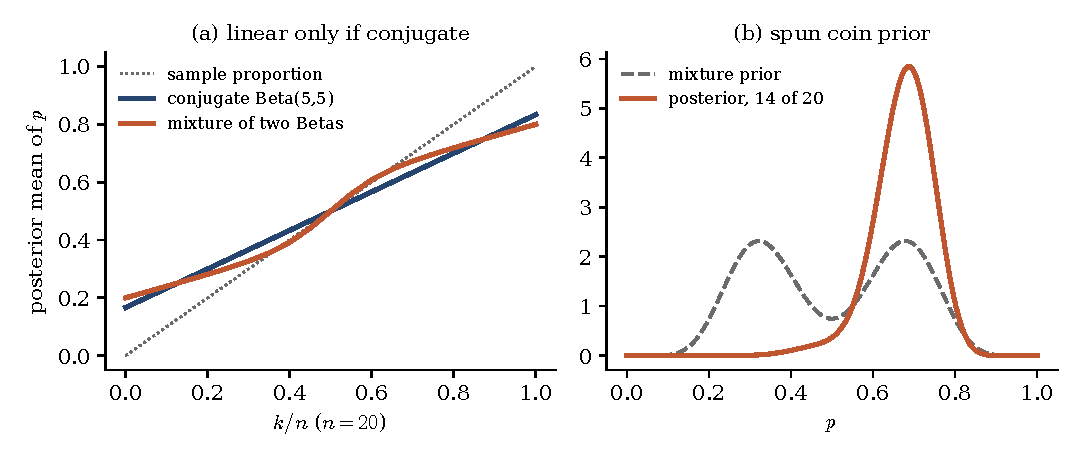
\includegraphics[width=0.95\textwidth]{dia_conjugate_linearity}
\caption{(a) Posterior mean of $p$ against the sample proportion for $n=20$: linear under a conjugate
prior, as Theorem~\ref{dia:thm:dy} requires, and nonlinear under a two component mixture. (b) The
bimodal spun coin prior and its posterior after $14$ heads in $20$ spins.}
\label{fig:dia_conj}
\end{figure}

\subsection{Applied examples: free throws and goals}\label{dia:sec:sports}

Efron and Morris (1975) shrank early season batting averages toward a common mean with a single normal
prior, so their shrinkage is linear (Section~\ref{ch:shrinkpics}). Free throw shooting shows why a
mixture is often the better prior. An analyst sees a new player make $k$ of $n$ free throws, and the
population is not unimodal: frontcourt players and guards shoot at visibly different rates. Take the
illustrative two type prior
\[
p\sim\tfrac12\mathrm{Beta}(65,35)+\tfrac12\mathrm{Beta}(84,16),
\]
a frontcourt type centered at $0.65$ and a guard type at $0.84$, each worth $100$ prior attempts. The
single Beta prior with the same mean and variance is $\mathrm{Beta}(12.3,4.2)$, centered at $0.745$ and
worth about $16.6$ attempts. Both say the same about the first two moments of $p$; they disagree about
its shape. The posterior odds on the guard type are the prior odds times a Bayes factor, a ratio of
conjugate normalizing constants,
\[
\frac{w_G(k)}{w_F(k)}=\frac{B(84+k,\,16+n-k)/B(84,16)}{B(65+k,\,35+n-k)/B(65,35)},
\]
so everything is exact. Table~\ref{tab:dia_ft} gives the numbers for $n=20$ and
Figure~\ref{fig:dia_sports} the picture.

\begin{table}[t]
\centering\small
\begin{tabular}{ccccc}
\toprule
Makes of 20 & Raw rate & $\Pb(\text{guard}\mid k)$ & Mixture mean & Single Beta mean\\
\midrule
$12$ & $0.60$ & $0.068$ & $0.652$ & $0.666$\\
$14$ & $0.70$ & $0.279$ & $0.702$ & $0.720$\\
$15$ & $0.75$ & $0.477$ & $0.742$ & $0.748$\\
$16$ & $0.80$ & $0.688$ & $0.784$ & $0.775$\\
$18$ & $0.90$ & $0.932$ & $0.839$ & $0.830$\\
\bottomrule
\end{tabular}
\caption{Free throws with $n=20$ attempts under the two type mixture prior and the moment matched
single Beta prior.}
\label{tab:dia_ft}
\end{table}

\begin{figure}[H]
\centering
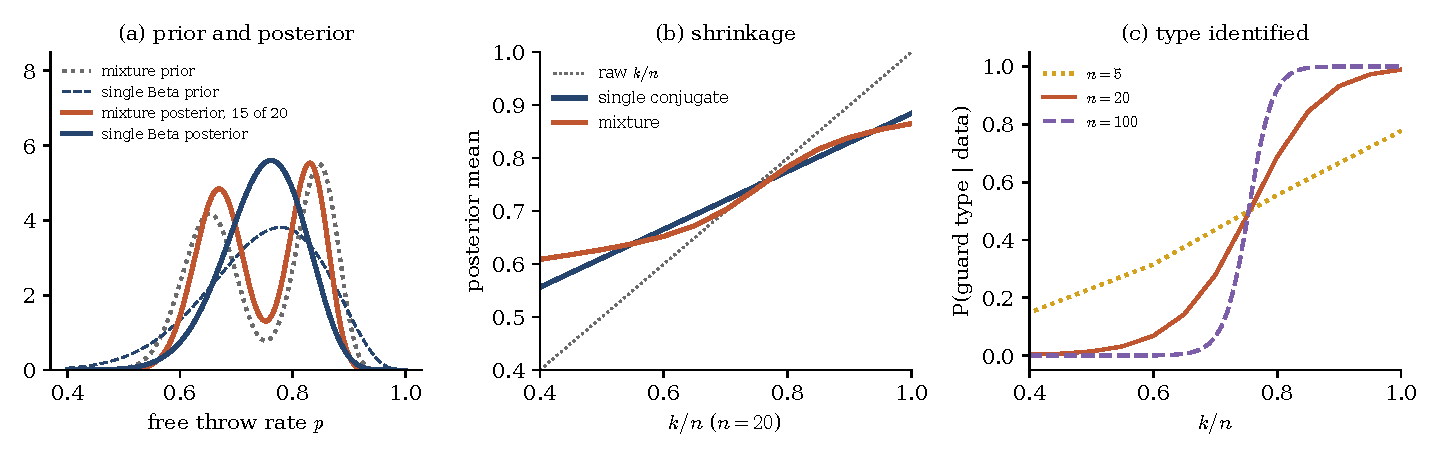
\includegraphics[width=\textwidth]{dia_sports_mixture}
\caption{Free throws with a two type mixture of conjugate priors. (a) Priors and posteriors after $15$
makes in $20$. (b) Posterior mean against the raw rate, $n=20$. (c) Posterior probability of the guard
type for $n=5$, $20$ and $100$ attempts.}
\label{fig:dia_sports}
\end{figure}

Three things are visible. After $15$ makes in $20$ the single Beta posterior is unimodal at about
$0.75$, while the mixture posterior is bimodal, with nearly equal weight on a player near $0.67$ and
one near $0.83$; the means nearly agree ($0.742$ against $0.748$), but the mixture is honest that the
player is probably one type or the other, and its $90$ percent interval $(0.610,0.867)$ is wider than
$(0.624,0.856)$. The mixture shrinks each player toward the type the data favors, so a player who
makes $12$ of $20$ is pulled to $0.652$ rather than $0.666$, and one who makes $18$ of $20$ only to
$0.839$ rather than $0.830$: shrinkage is adaptive. And the type is learned at a Sanov rate: the log
Bayes factor grows like $n$ times the difference of the two divergences from the empirical rate to
each type, so with $100$ attempts the classification is nearly a step function.

Counts work the same way. Let a team's goals per match be Poisson with rate $\lambda$, and before the
season let the team be a weaker side, $\lambda\sim\mathrm{Gamma}(12,10)$ with mean $1.2$, or a
stronger one, $\lambda\sim\mathrm{Gamma}(18,10)$ with mean $1.8$, with equal probability. After $11$
goals in $5$ matches the components update to $\mathrm{Gamma}(23,15)$ and $\mathrm{Gamma}(29,15)$,
with means $1.53$ and $1.93$, and the weights become $0.27$ and $0.73$. The mixture forecast is $1.82$
goals per match, and the moment matched single prior $\mathrm{Gamma}(9.4,6.25)$ gives $1.81$: almost
the same point forecast, but only the mixture also reports that the odds of a strong side have moved
from even to about $73$ percent, which is often what a coach or a bettor wants.

\subsection{Limitations, consistency, and updating}\label{dia:sec:limits}

Three caveats belong with conjugate priors. Conjugacy depends on the parametrization: a density of the
same form written in the mean parameter is in general a different prior, and Consonni and Veronese
(1992) show that the two constructions agree exactly for the natural exponential families with
quadratic variance function, the Morris class of normal, Poisson, gamma, binomial, negative binomial
and generalized hyperbolic secant laws. Linearity is not robust: in the normal case the posterior
mean moves by $n(\bar x-x_0)/(n_0+n)$ without bound however strongly the data conflict with the prior,
whereas under a heavy tailed prior the influence of the prior vanishes as $|\bar x-x_0|\to\infty$
(Dawid, 1973; Pericchi and Smith, 1992), which is the motivation for the horseshoe, a scale mixture
of conjugate normals designed to break linearity in the tails. And a single $n_0$ ties the prior
precision of every coordinate to one number, which hierarchical, conditionally conjugate priors
relax.

Consistency is a property of the prior and the model jointly. Diaconis and Freedman (1986) showed that
in the symmetric location problem with a Dirichlet process prior on the error law the posterior for
the location can be inconsistent, while for multinomial data with a Dirichlet prior the posterior is
consistent uniformly over the simplex (Diaconis and Freedman, 1990), the finite state case on which
the method of types rests. Section~\ref{ch:asymptotics} sets these beside Doob's and Schwartz's
theorems.

Diaconis and Zabell (1982) asked when a revision of belief from $P$ to $Q$ can be represented as
conditioning on an event in a richer space, and studied Jeffrey's rule, in which new information fixes
the probabilities $q_i$ of the cells $E_i$ of a partition without making any one certain:
$Q(A)=\sum_iq_iP(A\mid E_i)$. Jeffrey's rule is the minimizer of $\D{Q}{P}$ subject to $Q(E_i)=q_i$, so
Bayes conditioning, Jeffrey conditioning and maximum entropy updating sit inside one variational
principle, the same one as the conditional limit theorem.

\paragraph{Coin tossing.} Diaconis, Holmes and Montgomery (2007) modeled the physics of a tossed and
caught coin and predicted a small bias toward the side that started up, about $0.51$, from precession.
Barto\v{s} and coauthors (2025) collected $350{,}757$ flips from $48$ people and report
$\Pb(\text{same side})=0.508$ with $95$ percent credible interval $(0.506,0.509)$, together with
considerable variation between people, which is why their interval comes from a hierarchical model
rather than a single Beta. The conjugate reading is still instructive: with $n$ in the hundreds of
thousands, a Diaconis and Ylvisaker prior worth $n_0$ flips moves the posterior mean by the fraction
$n_0/(n_0+n)$ of the gap between its guess and the data, about $0.3$ percent of that gap even at
$n_0=1000$, so prior sensitivity has vanished and what remains is the between person heterogeneity.

\paragraph{Further reading.} Diaconis (2009) is the best short account of why Markov chain Monte Carlo
works and how fast, including the cutoff phenomenon and the seven shuffles of Bayer and Diaconis
(1992), an exact variation distance computation in the spirit of Figure~\ref{fig:dia_finite}. His
books with Graham (2012) and with Skyrms (2018), and his 1988 lecture notes on group representations,
cover shuffling, chance and symmetry at several levels. Diaconis (2023) on approximate exchangeability
and de Finetti priors, and Diaconis (2022) on partial exchangeability for contingency tables, point to
open problems on how far the representation extends.

\paragraph{Summary.}
For an exchangeable sequence of length $n$ with values in a set of $c$ elements, the law of the first $k$ coordinates lies within variation distance $ck/n$ of a mixture of i.i.d.\ laws, and within $k(k-1)/(2n)$ for a general state space (Theorem~\ref{dia:thm:finite}). Conditioning an i.i.d.\ exponential family sample on its sufficient statistic gives, for $k$ small relative to $n$, nearly the i.i.d.\ law at the exponential tilt, so the conditional limit theorem and de Finetti's theorem are one result read in two directions (Theorem~\ref{dia:thm:clt}). A prior that is not a point mass is conjugate if and only if the posterior mean of $m(\theta)$ is linear in the observation with nonzero slope (Theorem~\ref{dia:thm:dy}), and the conjugate prior and posterior are Gibbs measures whose energy is the divergence from an imaginary or pooled sample, \eqref{dia:eq:klprior}. Finite mixtures of conjugate priors keep closed form updating, approximate any prior, and give forecasts that are not linear in the data; conjugacy itself depends on the parametrization and is not robust to conflict between prior and data.

\subsection*{Problems}
\begin{enumerate}[leftmargin=2.2em,itemsep=2pt]
\item Show that the uniform law on $\{(0,1),(1,0)\}$ is exchangeable but is at variation distance at
least $\tfrac12$ from every mixture of i.i.d.\ Bernoulli laws.
\item Compute the exact variation distance between the hypergeometric and binomial laws of the first
$k$ draws from an urn of $n$ balls, half marked one. Show that it equals $1/(2(n-1))$ at $k=2$, and
compare it with $k/(4n)$ for $2\le k\le100$ when $n=10^4$.
\item Prove part (i) of Theorem~\ref{dia:thm:dy} and derive each row of Table~\ref{tab:dia_conj} by a change
of variables from $\theta$ to the usual parameter.
\item Verify \eqref{dia:eq:klprior} and show that the conjugate posterior is the inverse Sanov Gibbs
measure of Proposition~\ref{prop:invsanov} for the pooled type.
\item Recompute Table~\ref{tab:dia_ft}; then simulate players from two types and compare the calibration
of the mixture and of the moment matched single Beta, and repeat when players come from one type.
\item Show that Jeffrey's rule minimizes $\D{Q}{P}$ subject to $Q(E_i)=q_i$.
\end{enumerate}

\src{A reading guide to Diaconis's work for this book (Polson, note of 23 October 2026); Diaconis
(1977); Diaconis and Freedman (1980a, 1980b, 1986, 1987, 1988, 1990); Diaconis and Ylvisaker (1979,
1985); Diaconis and Zabell (1982); Zabell (1982); Dalal and Hall (1983); Consonni and Veronese (1992); Morris (1982);
Diaconis, Holmes and Montgomery (2007); Barto\v{s} and coauthors (2025); Gavalakis, Johnson and
Kontoyiannis (2024). All figures and numbers were recomputed for the book.}


%====================================================================================================

\chapter{Risk, Coding, and Shrinkage}\label{chap:risk}

With the synthesis in hand we can price inference in nats and read its economics. This chapter asks
three questions that turn out to be one. What is the Bayes risk of a decision, and where does the
optimal testing threshold sit? What is the shortest code for the data, and why does description length
reproduce the Bayesian evidence? And how should a high-dimensional signal be shrunk when most of its
coordinates are noise?

The answers all live on the moderate-deviation scale: the risk-optimal threshold, the coding penalty,
and the sparse-recovery boundary are the same $\sqrt{\log n}$ quantity seen from three sides. The
chapter culminates in the horseshoe prior, whose infinite spike at the origin and heavy tail are
the two features the moderate-deviation calculus rewards, and it shows why those features,
and not the details of any particular penalty, are what a sparse predictive rule requires.


\section{Bayes Risk: Calculations and Economics}\label{ch:risk}

\noindent\textbf{Thesis.} A screening study is a decision problem; the object that solves it is the
posterior odds, the threshold that calibrates it lives on the moderate-deviation scale, and the value
of each part of the decision can be priced.

\subsection{The decision and its expected loss}
Let $C_{\mathrm{FD}}$ and $C_{\mathrm{FND}}$ be the costs of a false discovery and a false
non-discovery, $R=C_{\mathrm{FND}}/C_{\mathrm{FD}}$, and $\mathrm{PO}=\pi_0/(1-\pi_0)$ the prior odds, where $\pi_0=\Pb(H_0)$ and $\pi_1=1-\pi_0$. The Bayes rule declares a marker noteworthy when the posterior odds on the null fall below $R$,
i.e.\ $\mathrm{ABF}\times\mathrm{PO}<R$, where the approximate Bayes factor with prior variance
$W=uV$ is $\mathrm{ABF}=\sqrt{1+u}\,\exp\{-\tfrac{z^2}{2}\cdot\tfrac{u}{1+u}\}$. Per marker, with
$z\sim\mathcal N(0,1)$ under $H_0$ and $\mathcal N(0,1+u)$ under $H_1$, the expected loss of the rule that declares a marker noteworthy when $|z|>z_c$ is
\begin{equation}\label{eq:loss}
L(z_c)=\pi_0\cdot 2\{1-\Phi(z_c)\}\,C_{\mathrm{FD}}+\pi_1\Bigl\{2\Phi\bigl(\tfrac{z_c}{\sqrt{1+u}}\bigr)-1\Bigr\}C_{\mathrm{FND}}.
\end{equation}
Setting $L'(z_c)=0$ gives the loss-minimizing threshold
\begin{equation}\label{eq:zT}
z_T^2=\Bigl(1+\tfrac1u\Bigr)\{\log(1+u)+2L\},\qquad L=\log(\mathrm{PO}/R),
\end{equation}
with a positive second derivative there, so \eqref{eq:zT} is a minimum, not merely the boundary of
the rule.

\subsection{The marginal density, Laplace, and the Schwarz criterion}
The decision above compares two models through an approximate Bayes factor; it is worth seeing where
that factor, and the $\tfrac12\log n$ it charges per parameter, come from. Bayesian model choice
compares models by their marginal density, or evidence,
\begin{equation}\label{eq:evidence}
m(x)=\int p(x\mid\theta)\,\pi(\theta)\,d\theta=\int e^{\ell_n(\theta)}\pi(\theta)\,d\theta,\qquad
\ell_n(\theta)=\log p(x\mid\theta),
\end{equation}
the probability the model assigns the data with the parameter integrated out (Wasserman, 2000). The
evidence rewards fit and penalizes flexibility on its own, since a model that spreads prior mass over
many parameter values must pay for the volume it does not use; this is the Bayesian form of Occam's
razor.

A Laplace approximation to \eqref{eq:evidence} makes the penalty explicit. For a model with $d$
parameters, expand $\ell_n$ about the maximum likelihood estimate $\hat\theta$, where
$\ell_n'(\hat\theta)=0$, to second order,
\[
\ell_n(\theta)\approx \ell_n(\hat\theta)-\tfrac{n}{2}(\theta-\hat\theta)^\top \bar j_n\,(\theta-\hat\theta),
\qquad \bar j_n=-\tfrac1n\ell_n''(\hat\theta)\to \mathcal I(\theta_0),
\]
with $\mathcal I$ the Fisher information. The Gaussian integral then gives
\[
m(x)\approx p(x\mid\hat\theta)\,\pi(\hat\theta)\,(2\pi)^{d/2}n^{-d/2}\lvert\bar j_n\rvert^{-1/2},
\]
so that, on the $-2\log$ scale,
\begin{equation}\label{eq:bic}
-2\log m(x)=\underbrace{-2\log p(x\mid\hat\theta)+d\log n}_{\text{Schwarz criterion (BIC)}}
\;-\;\underbrace{\bigl[\,2\log\pi(\hat\theta)+d\log(2\pi)-\log\lvert\bar j_n\rvert\,\bigr]}_{O(1)}+o(1).
\end{equation}
The leading two terms are the Schwarz criterion (Schwarz, 1978): each parameter is charged
$\tfrac12\log n$ of description length. That charge is what a fixed $p$-value threshold declines
to pay, and it is the source of the $\sqrt{\log n}$ threshold in \eqref{eq:zT}; it is the sense in
which the approximate Bayes factor is, as the next subsection puts it, BIC in disguise.

\paragraph{Jeffreys' prior and the Shannon information.} The $O(1)$ remainder in \eqref{eq:bic} is not
noise; it records the prior. Choosing Jeffreys' prior $\pi(\theta)\propto\lvert\mathcal
I(\theta)\rvert^{1/2}$ makes the prior-dependent part $2\log\pi(\hat\theta)-\log\lvert\bar j_n\rvert$
reduce asymptotically to the constant $-2\log c$, with $c$ the normalizing constant of $\pi$, since $\bar j_n\to\mathcal I(\theta_0)$, leaving an evidence that is invariant to
reparametrization and privileges no coordinate system. The deeper reason is information-theoretic:
Polson (1988) gives the asymptotic expansion of the Shannon information of the posterior and shows that
Jeffreys' prior is the one maximizing the expected information the experiment provides, which is why it
is the reference prior in the one-parameter case (Clarke and Barron, 1994). Evidence penalty, reference
prior, and Fisher information are three readings of the same second-order term.

\paragraph{Information and design.} That expected information is Lindley's. Lindley (1956) defined the
information provided by an experiment $\mathcal E$ under prior $\pi$ as the expected Kullback--Leibler
divergence from prior to posterior,
\[
I(\mathcal E,\pi)=\E_{x}\,\D{\pi(\cdot\mid x)}{\pi}=I(\theta;X),
\]
the mutual information between parameter and data, and used it to compare and to design experiments. It
accumulates over independent replications like $\tfrac{d}{2}\log n$, the same term
the Laplace expansion charges: the Schwarz penalty and Lindley's information are the coding and the
design faces of one quantity. Prior choice, model choice, and experimental design are thus governed by a
single second-order information expansion, a theme
Section~\ref{ch:asymptotics} develops in full.


\subsection{The Schwarz identity and the e-value}
The ABF is BIC in disguise:
\[
-2\log\mathrm{ABF}=z^2\,\frac{u}{1+u}-\log(1+u)=z^2-\log(K^\star n)+O(n^{-1}),
\]
where $u=K^\star n$ with $K^\star=W/(nV)$ a constant (the prior variance $W$ is fixed while the sampling variance $V$ falls like $1/n$) and $z$ fixed, so the $\tfrac12\log n$ that BIC charges per parameter is what a fixed $p$-value threshold
declines to pay. Independently of the prior, the reciprocal ABF is an e-value: for any proper prior
$g$ on the standardized effect, $\E_{H_0}[\mathrm{ABF}^{-1}]=1$, so
$\Pb_{H_0}(\mathrm{ABF}^{-1}\ge1/\alpha)\le\alpha$ by Markov's inequality, the product across
independent studies is an e-value, and the running product is a nonnegative $H_0$-martingale, so
Ville\index{Ville's inequality}'s inequality gives a bound that survives optional stopping. Evidence reported on the ABF scale
carries no penalty for looking, which is what makes the sequential design of Section~\ref{ch:evalues}
anytime-valid.

\subsection{Why the threshold is a moderate deviation}
Three scales must be distinguished for a studentized statistic $z_n$ from $n$ subjects. At a fixed
level the central limit theorem applies with additive error $O(n^{-1/2})$, useless against a target
probability of order $10^{-8}$. At a level proportional to $\sqrt n$ the large-deviation rate
$I(x)$ depends on the entire sampling distribution and is not universal. At a level growing slowly,
$1\ll b_n\ll\sqrt n$, the moderate-deviation principle gives
$b_n^{-2}\log\Pb(|z_n|\ge b_n x)\to-x^2/2$, the Gaussian rate function \emph{whatever} the underlying
distribution. A genome-wide threshold grows only logarithmically, $z_T\asymp\{\log(m^2 n)\}^{1/2}$,
so it lives permanently in the moderate zone; as studies grow, $\sqrt n$ races away and the threshold
sinks deeper into it. Universality is what licenses a summary-statistic Bayes factor: a procedure
that sees the data only through $z$ loses nothing at the scale that matters, even though $z$ is not
sufficient. The license is not free. The moderate-deviation approximation is valid in relative error
only while $\log(m^2 n)=o(n^{1/3})$ (Fan, Hall and Yao, 2007); the finite-sample diagnostic $\delta_n=(1+z_T)^3/\sqrt n$ flags
where the Gaussian calibration is being used outside the zone the theory endorses, and where one
should lean instead on the e-value bound, which is Markov's inequality and needs no tail
approximation.

\subsection{The threshold law, and Jeffreys' precedent}
Expanding \eqref{eq:zT} gives $z_T^2=\log u+2L+O(u^{-1}\log u)$ and hence, for the threshold $p$-value $p_T=2\{1-\Phi(z_T)\}$, $\log_{10}p_T=-\tfrac12\log_{10}n-\tfrac12\log_{10}\log n+O(1)$: the threshold falls with sample size
like $n^{-1/2}$, up to a logarithm. Under a power prior $\pi_0=\Pi_0^{1/m}$ the multiplicity enters
as $\log_{10}p_T=-\log_{10}m-\tfrac12\log_{10}n-\tfrac12\log_{10}\log(m^2 n)+O(1)$: Bonferroni supplies
the $m$ and omits the $\sqrt n$. The expected number of false discoveries then vanishes at rate
$n^{-1/2}$, whereas under a fixed Bonferroni threshold it is the constant $\alpha$ forever; this is
the Jeffreys--Lindley\index{Lindley's paradox} phenomenon in the currency a geneticist cares about. The $\sqrt{\log n}$ law is
not new: Jeffreys (1936) derived it, tabulated the critical values at which his Bayes factor equals
one, and it has stood in every edition of \emph{Theory of Probability} since (Jeffreys, 1961). The profession adopted
a constant threshold anyway.

\subsection{The moderate-deviation scale for testing}
The same scale governs Bayes-risk-optimal testing quite generally. Under integrated Bayes risk with
fixed prior weights and non-adaptive thresholds, the risk-optimal rejection boundary lies at
$n\lambda_n^2\asymp\log n$, with $\lambda_n=|\hat\theta-\theta_0|$ the deviation of the estimate from the null value (Section~\ref{ch:deviations}), giving critical values of order $\sqrt{\log n}$, a square-root
logarithmic inflation over the local-asymptotic-normal scale and in contrast to the
sample-size-invariant calibration of classical testing. For goodness of fit, the classical
statistics, Kolmogorov--Smirnov, likelihood-ratio, Pearson $\chi^2$, and entropy-deficit, differ in how fast their null tails decay at the value typical of the true law: by Sanov's theorem the exponent is at most, and for the likelihood ratio of the true law to the null equal to, the
Sanov rate $\D{G}{F_0}$ ($G$ the true law, $F_0$ the null), and Bayes-risk calibration places them on the moderate-deviation scale with
the same $\sqrt{\log n}$ inflation and polynomially decaying Type~I error. Risk, not the choice of
statistic, selects the regime.

\subsection{The economics, and the winner's curse}
Because this is a decision problem, the value of getting each part right can be stated; the values below are those reported for the genome-wide study of Polson, Sokolov and Zantedeschi (2026e). \emph{Design}
is worth about $32\times$: a two-stage genotyping design optimized by a Bellman recursion, carrying a
fraction of markers forward and spending most of the budget at stage one, yields on the order of
thirty times the expected true discoveries of a single-stage design of equal cost. The \emph{winner's
curse} is worth about sixteen points of replication power: among selected markers the maximum
likelihood estimate overstates the effect, and since the required sample size scales as the inverse squared effect, a
replication sized for $80\%$ power at the estimate (a two-sided test at level $5\%$) is in fact powered near $64\%$ when the true effect is about $83\%$ of the estimate; reporting the posterior mean removes
the inflation. The \emph{threshold}, the quantity the literature has argued about for two decades, is
worth only a few percent of expected loss and vanishes at biobank scale. \emph{Validity} is not
priced at all when the e-value bound is used, since it invokes no tail approximation. The winner's
curse is itself an instance of the machinery of Section~\ref{ch:sanov}: by the Gibbs conditioning principle,
conditionally on a marker being declared, its data resemble the nearest point of the rejection
region, the I-projection onto the selection event, and the correction is Tweedie\index{Tweedie's formula}'s formula, the same
posterior-mean shrinkage the ABF prior induces.
%%---- bridge: Bayes testing (full treatment in ch:evalues and ch:deviations) ----
\subsection{A New Look at Bayes Testing}
\label{sec:bayes-testing}

Two questions organize Bayesian testing, and each has a sharp moderate-deviation
answer developed in full later in the book. Fixing the sample size, the risk-optimal
Bayes-factor boundary sits at $t^2_{\mathrm{crit}}=\log n+O(1)$, a $\sqrt{\log n}$
inflation above the classical scale, with universal leading term and prior-sensitive
constants; this is the subject of Section~\ref{ch:deviations}, together with the
three deviation regimes, the Lindley paradox as a scale mismatch, the BIC
connection, and the exponential-family extension. Letting data accrue instead, the
likelihood-ratio E-process crosses a fixed evidence level $b$ after
$\E_{P_1}[\tau_b]=(\log b)/\D{P_1}{P_0}+O(1)$ observations;
this, with the typed representation/validity/decision calculus, the canonicality of
the likelihood ratio under log-loss, and the code-to-E obstruction, is the subject
of Section~\ref{ch:evalues}. The two thresholds are one phenomenon read on two axes:
both live at the moderate-deviation scale where Gaussian tails decay polynomially,
both separate a universal $\log$ term from prior- and model-dependent constants, and
both stand against fixed-threshold alternatives, the classical $z_{1-\alpha/2}$ and
the fixed-sample Markov $\sqrt{2\log(1/\alpha)}$, that do not grow with the data.




\subsection*{Worked example: Lindley's paradox end to end}
This example computes, in one place, why a fixed significance level and a Bayes factor can point in opposite directions.

Test $H_0:\theta=0$ against a $\N(0,1)$ alternative prior from $\bar X_n\sim\N(\theta,1/n)$. The marginal under the alternative is $\N(0,1+1/n)$, so the Bayes factor is $BF_{01}=\sqrt{1+n}\,\exp\{-\tfrac{n\bar x^2}{2}\cdot\tfrac{n}{n+1}\}$. Setting $BF_{01}=1$ gives the rejection boundary $t^2=\bar x^2 n=\tfrac{n+1}{n}\log(1+n)$, i.e.\ $t_{\mathrm{crit}}=\sqrt{\log n}\,(1+o(1))$. At $n=100$ this is $t_{\mathrm{crit}}\approx2.16$, already above the classical $1.96$: an observation at $z=1.96$ gives $BF_{01}\approx1.50$, mild evidence \emph{for} $H_0$. This is Lindley's paradox computed end to end.

The numbers make the collision vivid. At $n=100$ the Bayes factor equals one at $t_{\mathrm{crit}}\approx2.16$, so the very observation $z=1.96$ that a frequentist rejects at the five-percent level returns a Bayes factor near $1.5$ in favor of the null, mild but genuine evidence the other way. The reason is structural: the alternative must spread its unit of prior mass across a whole range of effect sizes, and at $n=100$ most of that range predicts the data worse than the sharp null does. The larger the sample, the more of the alternative's mass is wasted on effects the data have ruled out, and the higher the Bayes factor sets its bar.

The moral is not that one procedure is wrong but that they answer different questions: the $p$-value asks how surprising the data are under $H_0$, while the Bayes factor asks which hypothesis predicts them better, and the second carries a $\sqrt{\log n}$ penalty the first never pays. The gap widens without bound as $n$ grows, so the paradox is a feature of scale, not a numerical accident.

\paragraph{Summary.}
Bayes risk under $0/1$ loss decomposes into prior-weighted Type~I and Type~II errors, and minimizing it produces a Bayes-factor threshold rule. On the moderate-deviation scale the risk-optimal boundary is $t^2_{\mathrm{crit}}=\log n+O(1)$, which is Jeffreys' threshold, the BIC penalty, and Lindley's paradox read from one calculation. The Bayes factor is an e-variable under the mixture null, $\E_{M_0}[BF_{10}]=1$.

\subsection*{Problems}
\begin{enumerate}[leftmargin=2.2em,itemsep=2pt]
\item For $\bar X_n\sim\N(\theta,\sigma^2/n)$, compute the integrated Bayes risk of a threshold rule and minimize it over the threshold.
\item Show that the Bayes factor satisfies $\E_{M_0}[BF_{10}]=1$, so it is an e-variable, and state the resulting Ville bound.
\item Derive the $\sqrt{\log(\pi n/2)}$ cutoff for a Cauchy prior at equal prior odds and verify the crossover with the classical $1.96$.
\item Explain Lindley's paradox quantitatively: find the sample size at which $t=1.96$ first favors $H_0$.
\item Relate the $(d/2)\log n$ BIC penalty to the Laplace expansion of the marginal likelihood used in the threshold.
\end{enumerate}

\src{Bayes Factors and Moderate Deviations in Genome-Wide Screening (Polson, Sokolov and Zantedeschi, 2026e); Bayes Risk for Goodness of
Fit Tests (2602.15297); A New Look at Bayesian Testing (2602.11132); Bayes, E-values, and Testing
(2602.04146); E-Values, Bayes Risk, Dual Role of Markov's Inequality (2604.00337).}

%====================================================================================================

\section{Nonparametric Predictive Bayes Risk}\label{ch:nonparametric}

\noindent\textbf{Thesis.} Placing the prior on the infinite-dimensional space of
distributions rather than on a finite parameter changes nothing essential about the
predictive decomposition of this book, and reveals its cleanest instance. The
Bayes predictive KL risk of a nonparametric procedure splits into a Sanov floor,
the Kullback--Leibler divergence from the truth to its reverse $I$-projection onto the
prior support, and a posterior-contraction term whose price of adaptation is, heuristically,
set by the Rubin--Sethuraman moderate-deviation scale of Section~\ref{ch:hsmdp}. The
floor is the divergence to the tilted de Finetti limit of Section~\ref{ch:projected} when the prior support is the exponential family that a moment constraint generates, now
read as the irreducible cost of misspecification; the contraction term is the rate
at which a Dirichlet-process mixture, a P\'olya\index{P\'olya tree} tree, or a logistic-Gaussian
process approaches it. The empirical distribution function is the nonparametric
conditioning statistic, so the predictive risk factors through the prior on CDFs
by Fubini, and the Kolmogorov--Smirnov-truncated predictive density is conjectured (Conjecture~\ref{np:conj:ks-mdp}) to inherit a
moderate-deviation truncation level of order $\sqrt{\log n}$ at the detection boundary. This section is the predictive-rate
apex of the framework: where Sections~\ref{ch:projected} and~\ref{ch:moment}
identify the predictive limit, it identifies the rate of approach.

\subsection{Setup}\label{np:sec:setup}

\textbf{Notation.} $\X = [0,1]$; $\M(\X)$ denotes Borel probability measures in the weak topology. For $P \in \M(\X)$ with Lebesgue density $p$, we write $F$ for the CDF. We use $\KL(P\|Q) = \int p\log(p/q)\,dx$, squared Hellinger $\dH^2(P,Q) = \tfrac{1}{2}\int(\sqrt{p}-\sqrt{q})^2\,dx$, and $\chi^2(P\|Q) = \int (p/q-1)^2 q\,dx$. $F_n$ is the empirical CDF.

\begin{assumption}[Bounded density]\label{np:ass:density}
$P_0$ has density $p_0$ with $0 < c_0 \le p_0 \le C_0 < \infty$ on $\X$.
\end{assumption}

\begin{assumption}[Hölder smoothness]\label{np:ass:holder}
$\log p_0 \in \mathcal{H}^\beta(L)$ for some $\beta \in (0, B]$, $L < \infty$.
\end{assumption}

\begin{assumption}[Convex prior support, unique reverse I-projection]\label{np:ass:convex}
$\supp(\Pi) \subset \M(\X)$ is convex and KL-closed; the map $P \mapsto \KL(P_0\|P)$ on $\supp(\Pi)$ attains its infimum at a unique element
\[
\Pi^*P_0 \;:=\; \argmin_{P\in\supp(\Pi)} \KL(P_0\|P).
\]
We write $\pi^*$ for the Lebesgue density of $\Pi^*P_0$, assumed to satisfy $c_0 \le \pi^* \le C_0$ with the constants of Assumption~\ref{np:ass:density}, and $F_\Pi^*$ for its CDF.
\end{assumption}

\begin{assumption}[Hellinger contraction]\label{np:ass:contraction}
There exist $\eps_n \to 0$ with $n\eps_n^2 \to \infty$ and constants $M, c > 0$ such that
\[
\Pi\!\bigl(\{P : \dH(P,\Pi^*P_0) > M\eps_n\} \mid X^{(n)}\bigr) \;\le\; e^{-cn\eps_n^2}
\]
in $P_0^{\otimes n}$-probability.
\end{assumption}

\begin{assumption}[Wong--Shen (1995)]\label{np:ass:wongshen}
There exist $\eta > 0$, $M_{\rm WS} \ge 1$ and $C_{\rm WS} < \infty$ such that for every $P$ with $\dH(P,\Pi^*P_0) \le \eta$ and $\pi^* \le M_{\rm WS}\,p$,
\[
\KL(\pi^*\|p) \;\le\; C_{\rm WS}\,\dH(P,\Pi^*P_0)^2.
\]
\end{assumption}

Here $\supp(\Pi)$ is the Kullback--Leibler support of $\Pi$, the set of laws $P$ with $\Pi\{Q : \KL(P\|Q) < \delta\} > 0$ for every $\delta > 0$, so that $P_0 \in \supp(\Pi)$ is the Kullback--Leibler property of $\Pi$ at $P_0$. Support in the weak topology does not suffice: a Dirichlet process whose base measure has full support has full weak support, yet $\KL(P_0\|P) = \infty$ for almost every draw (Example~\ref{np:ex:dp-iproj}). Assumption~\ref{np:ass:convex} posits the reverse I-projection rather than deriving it; Csisz\'ar (1975) minimizes $\KL$ over its first argument, whereas $\Pi^*P_0$ minimizes over the second. On a convex support of laws with densities the uniqueness is automatic, since $p \mapsto -\int p_0\log p\,dx$ is strictly convex where $p_0 > 0$, which under Assumption~\ref{np:ass:density} is all of $\X$. Assumption~\ref{np:ass:contraction} is the standard posterior-contraction assumption (Ghosal, Ghosh and van der Vaart, 2000); for the example priors, Theorems~\ref{np:thm:dp}--\ref{np:thm:gp} reach the Hölder rate $\eps_n = n^{-\beta/(2\beta+1)}$, up to polylog factors, only under hypotheses stated in each theorem. Assumption~\ref{np:ass:wongshen} converts Hellinger to KL contraction, and its ratio bound $\pi^* \le M_{\rm WS}\,p$ makes it hold for every prior and every $\eta$, with $C_{\rm WS} = 4 + 2\log M_{\rm WS}$: with $r = \pi^*/p$, $\KL(\pi^*\|p) = \int p\,(r\log r - r + 1)\,dx$ and $2\dH^2(P,\Pi^*P_0) = \int p\,(\sqrt r - 1)^2\,dx$, while $r\log r - r + 1 \le (2 + \log M_{\rm WS})(\sqrt r - 1)^2$ for $0 \le r \le M_{\rm WS}$. Without the ratio bound the condition fails at $\pi^*$ with a short interval cut out and renormalized, a density Hellinger-close to $\pi^*$ with $\KL(\pi^*\|p) = \infty$; such densities are left to the tail condition of Theorem~\ref{np:thm:master}.

\subsection{Predictive Bayes Risk}\label{np:sec:abc}

We now develop the central decomposition of the section. The story unfolds in three pieces: (i) the predictive density and its log-loss, with classical foundations; (ii) the Aitchison--Barron--Clarke chain rule pivoted at the reverse I-projection; and (iii) the decomposition theorem with its cross-term bound.

\subsubsection{The Bayes predictive density and KL risk}\label{np:sec:abc-bayes-pred}

For a prior $\Pi$ on $\M(\X)$, the Bayes predictive density $\hat p_\Pi(\cdot \mid X^{(n)})$ is the posterior mean of the candidate density,
\begin{equation}\label{np:eq:abc-pred}
\hat p_\Pi(y \mid X^{(n)}) \;=\; \int p(y)\,\Pi(dP \mid X^{(n)}).
\end{equation}
This is the Bayes-optimal predictor under log loss: among all conditional densities $q(\cdot\mid X^{(n)})$ measurable w.r.t.\ $X^{(n)}$, $\hat p_\Pi$ uniquely minimizes the Kullback--Leibler risk averaged over the prior,
\[
\int \E_{P^{\otimes n}}\,\KL\!\bigl(p\,\|\,q(\cdot \mid X^{(n)})\bigr)\,\Pi(dP),
\]
whenever this risk is finite for some $q$. Its risk at a fixed truth $P_0$, $R_{\KL}(P_0;\hat p_\Pi) := \E_{P_0^{\otimes n}}\KL\bigl(p_0\,\|\,\hat p_\Pi(\cdot \mid X^{(n)})\bigr)$, is the \emph{predictive Bayes risk}: the frequentist risk of the Bayes rule at $P_0$, not a minimum over $q$.

For parametric models, classical asymptotics (Aitchison, 1975; Clarke and Barron, 1990) decompose the risk summed over the first $n$ predictions into a deterministic $(d/2)\log n$ second-order term (the parametric Bayes-risk floor) plus a remainder controlled by the prior at the truth. Clarke and Barron (1994) further show that the Jeffreys prior is asymptotically least favorable under entropy risk. For nonparametric models, the situation is more delicate: the prior is supported on an infinite-dimensional space, the second-order term is governed by smoothness and adaptive penalties, and, crucially, the prior support may not contain the true $P_0$. The decomposition below addresses both well- and misspecified settings simultaneously (for the misspecified case see Kleijn and van der Vaart, 2006).

\subsubsection{The Aitchison--Barron--Clarke chain-rule identity}\label{np:sec:abc-chain}

The fundamental identity, due in essence to Aitchison (1975) and made central in Barron (1988) and Clarke--Barron (1990), is the chain rule for relative entropy: for any reference density $q$ on $\X$ with $\KL(p_0\|q) < \infty$,
\begin{equation}\label{np:eq:abc-chain}
\KL(p_0\|\hat p) \;=\; \KL(p_0\|q) \;+\; \E_{Y\sim p_0}\!\left[\log\frac{q(Y)}{\hat p(Y)}\right].
\end{equation}
The identity holds path-wise for every realization of $X^{(n)}$. Two choices of reference density are noteworthy. With $q = p_0$, the identity collapses to the (positive) cross-entropy expression $\KL(p_0\|\hat p) = -\E_{p_0}\log\hat p - H(p_0)$, classical in information theory but unhelpful for non-asymptotic analysis. With $q = \pi^*$, the density of the reverse I-projection $\Pi^*P_0$ (Assumption~\ref{np:ass:convex}), the first term becomes a population quantity, the \emph{Sanov rate} $\KL(P_0\|\Pi^*P_0)$, which is constant in $n$ and vanishes precisely when $P_0 \in \supp(\Pi)$. The second term, after a change of measure, decomposes into a contraction term and a cross term.

\subsubsection{Decomposition theorem}\label{np:sec:abc-theorem}

The pivot $q = \pi^*$ makes the first term population (the Sanov rate) and the second asymptotically vanishing. We make the cross term explicit via Csisz\'ar's I-divergence geometry.

\begin{theorem}[Decomposition of nonparametric predictive Bayes risk]\label{np:thm:abc-csiszar}
Under Assumptions~\ref{np:ass:density}--\ref{np:ass:wongshen},
\begin{equation}\label{np:eq:master}
R_{\KL}(P_0;\hat p_\Pi) \;=\; \underbrace{\KL(P_0\|\Pi^*P_0)}_{\text{Sanov term}} \;+\; \underbrace{J_n(\Pi,P_0)}_{\text{contraction term}} \;+\; r_n,
\end{equation}
where $J_n(\Pi,P_0) := \E_{P_0^{\otimes n}}\KL(\Pi^*P_0\|\hat p_\Pi)$ and the cross term satisfies
\begin{equation}\label{np:eq:cross}
|r_n| \;\le\; C\,\Bigl(\sqrt{\KL(P_0\|\Pi^*P_0)\cdot J_n(\Pi,P_0)} \;+\; J_n(\Pi,P_0)\Bigr),
\end{equation}
with $C = e\,C_0/c_0$ whenever $\pi^* \ge c_0$. Asymptotically, when $J_n(\Pi,P_0)\to0$ (Theorem~\ref{np:thm:master} gives $J_n=O(\eps_n^2)$ under its tail condition):
\begin{itemize}
\item if $\KL(P_0\|\Pi^*P_0) > 0$ (\emph{misspecified}): $R_{\KL}(P_0;\hat p_\Pi) = \KL(P_0\|\Pi^*P_0)\,(1+o(1))$;
\item if $\KL(P_0\|\Pi^*P_0) = 0$ (\emph{well-specified}): $R_{\KL}(P_0;\hat p_\Pi) = J_n(\Pi,P_0)\,(1+o(1))$.
\end{itemize}
\end{theorem}

\begin{proof}
Apply \eqref{np:eq:abc-chain} with $q = \pi^*$, take $P_0^{\otimes n}$-expectation, and change measure on the second term:
\[
\E_{Y\sim p_0}\!\left[\log\frac{\pi^*(Y)}{\hat p_\Pi(Y)}\right]
\;=\; \KL(\pi^*\|\hat p_\Pi) \;+\; \E_{Y\sim\pi^*}\!\left[\!\left(\tfrac{p_0(Y)}{\pi^*(Y)}-1\right)\log\tfrac{\pi^*(Y)}{\hat p_\Pi(Y)}\right].
\]
The first term, after $P_0^{\otimes n}$-expectation, is the contraction term $J_n$. The part of the cross term on the set $A := \{\hat p_\Pi \ge \pi^*/e\}$ is bounded in absolute value by Cauchy--Schwarz:
\[
\left|\E_{Y\sim\pi^*}\!\left[\!\left(\tfrac{p_0}{\pi^*}-1\right)\log\tfrac{\pi^*}{\hat p_\Pi}\,\1_A\right]\right|
\;\le\; \sqrt{\chi^2(P_0\|\Pi^*P_0)\,\cdot\,V_n},
\]
where $V_n := \E_{Y\sim\pi^*}[(\log(\pi^*/\hat p_\Pi))^2\,\1_A]$. Since $p_0 \le C_0$ and $\pi^* \ge c_0$, the elementary inequality $\chi^2(P\|Q) \le 2\sup_x(p/q)\cdot \KL(P\|Q)$ (valid for any $P\ll Q$ with bounded ratio) gives $\chi^2(P_0\|\Pi^*P_0) \le 2(C_0/c_0)\,\KL(P_0\|\Pi^*P_0)$. Write $w := \hat p_\Pi/\pi^*$ and $\phi(w) := w-1-\log w \ge 0$, so that $\KL(\pi^*\|\hat p_\Pi) = \E_{Y\sim\pi^*}[\phi(w)]$ (as $\E_{Y\sim\pi^*}[w-1] = 0$). On $A$, where $w \ge 1/e$, $(\log w)^2 \le e\,\phi(w)$, so $V_n \le e\,\KL(\pi^*\|\hat p_\Pi)$; off $A$, $|\log w| \le e\,\phi(w)$ and $|p_0/\pi^*-1| \le C_0/c_0$, so the part of the cross term off $A$ is at most $e\,(C_0/c_0)\,\KL(\pi^*\|\hat p_\Pi)$ in absolute value. Taking $P_0^{\otimes n}$-expectation, with Jensen's inequality for the square root, yields \eqref{np:eq:cross} with $C = e\,C_0/c_0$, since $C_0/c_0 \ge 1$ gives $\sqrt{2e\,C_0/c_0} \le e\,C_0/c_0$. The asymptotic dichotomy follows: in the misspecified regime, $\KL(P_0\|\Pi^*P_0) > 0$ is fixed while $J_n \to 0$ (by hypothesis, as under Theorem~\ref{np:thm:master}); hence $|r_n| = O(\sqrt{J_n}) = o(1)$ and the Sanov term dominates. In the well-specified regime, $P_0 = \Pi^*P_0$ and the change-of-measure identity reduces to $\KL(p_0\|\hat p_\Pi) = \KL(\pi^*\|\hat p_\Pi)$ pathwise, giving $r_n = 0$ identically.
\end{proof}

\begin{remark}[Csisz\'ar Pythagorean equality]\label{np:rem:csiszar}
When $\supp(\Pi)$ is an exponential family $\{p_\lambda \propto \exp(\sum_{j=1}^k \lambda_j h_j)\}$ for fixed sufficient statistics $h_j$ and some member $\pi^*$ satisfies $\int \pi^*\,h_j\,dx = \int p_0\,h_j\,dx$ for every $j$, that member is the minimizer $\Pi^*P_0$ and the cross term vanishes at the population level:
\begin{equation}\label{np:eq:pythagorean}
\KL(P_0\|P) \;=\; \KL(P_0\|\Pi^*P_0) \;+\; \KL(\Pi^*P_0\|P), \qquad \forall\, P \in \supp(\Pi).
\end{equation}
Identity \eqref{np:eq:pythagorean} is the reverse-direction analogue of the Pythagorean equality for I-projections onto a linear family such as $\{p : \int p\,h_j\,dx = c_j,\ j = 1,\dots,k\}$, where the minimization is over the first argument (Csisz\'ar, 1975, Theorem~3.2); it expresses that the reverse I-projection $\Pi^*P_0$ is the unique element of $\supp(\Pi)$ whose deviation from $P_0$ is ``orthogonal'' (in the Fisher-information sense) to all variations within the support. For a linear (mixture) family, minimized over the second argument, \eqref{np:eq:pythagorean} need not hold: the one-parameter cosine family of the worked example of Section~\ref{np:sec:miss-example} is of this kind, and there the identity holds to leading order (Section~\ref{np:sec:ex-geometry}), giving a cross term of smaller order and explaining why the Cauchy--Schwarz bound \eqref{np:eq:cross} is loose for that example (see Remark~\ref{np:rem:ex-cross}).
\end{remark}

\begin{remark}[Comparison with parametric Clarke--Barron asymptotics]\label{np:rem:clarke-barron-comparison}
For parametric Bayes prediction under a smooth $d$-dimensional model with prior $\pi$ in the interior of the support, Clarke and Barron (1990) prove, for the Bayes risk averaged over the first $n$ predictions,
\[
R_{\KL,\text{parametric}}(P_0;\hat p_\pi) \;=\; \frac1n\Bigl\{\frac{d}{2}\log\!\frac{n}{2\pi e} \;+\; \frac{1}{2}\log\!\det\mathcal I(P_0) \;-\; \log\pi(P_0)\Bigr\} \;+\; o(1/n).
\]
The leading $(d/2)\log n / n$ term comes from averaging over the first $n$ predictions the risk $d/(2k)\,(1+o(1))$ of the prediction from $k$ observations. It is that single-prediction risk at sample size $n$, the quantity $R_{\KL}$ of Theorem~\ref{np:thm:abc-csiszar}, that corresponds in our nonparametric framework to the contraction term $J_n$ (Proposition~\ref{np:prop:ex-contraction} gives $J_n = (1+o(1))/(2n)$ at $d = 1$), with $\eps_n^2 \asymp 1/n$ for finite-dimensional models. The Sanov term \emph{vanishes} for parametric models with prior support containing the truth: parametric well-specification is the special case $\KL(P_0\|\Pi^*P_0) = 0$ of our decomposition. The Clarke--Barron Jeffreys-prior asymptotic optimality (Clarke and Barron, 1994) concerns the dependence of the second-order constants on the prior; our framework is at a more crude rate level and is consistent with their refinement.
\end{remark}

\begin{remark}[The two regimes in practice]\label{np:rem:two-regimes}
The dichotomy in Theorem~\ref{np:thm:abc-csiszar} has a sharp interpretation for the practitioner. \emph{Well-specified}: the support of $\Pi$ contains the true $P_0$ (for instance, $\Pi$ is a Dirichlet process\index{Dirichlet process} mixture or a P\'olya tree whose Kullback--Leibler support contains the bounded density $P_0$, as in Examples~\ref{np:ex:dp-iproj} and~\ref{np:ex:pt-iproj}). The predictive risk is at most of order $\eps_n^2$, the squared contraction rate, which for adaptive priors includes polylog factors (Theorem~\ref{np:thm:master}). \emph{Misspecified}: the support of $\Pi$ does not contain $P_0$ at the population level. Then the predictive risk has an \emph{irreducible floor} equal to $\KL(P_0\|\Pi^*P_0) > 0$, regardless of sample size. Theorem~\ref{np:thm:abc-csiszar} makes this floor computable: $\Pi^*P_0$ is the unique reverse I-projection of $P_0$ onto the prior support, and its closed form is available for the three standard priors (Examples~\ref{np:ex:dp-iproj}--\ref{np:ex:lgp-iproj}). The diagnostic of computing the reverse I-projection and inspecting whether $\KL(P_0\|\Pi^*P_0)$ is zero or positive is the principal applied content of the theorem.
\end{remark}

\subsection{The Sanov Term and Tilted de Finetti}\label{np:sec:sanov}

\begin{theorem}[Conditional Sanov / tilted de Finetti, Polson and Zantedeschi (2025a, Thm.~3.1)]\label{np:thm:tilted}
Let $\{X_i\}$ be infinitely exchangeable with de Finetti mixing measure $\Pi$, and $E \subset \M(\X)$ closed convex with $\inf_{P\in E}\KL(P\|\Pi^\dagger) < \infty$ for de Finetti baseline $\Pi^\dagger$. Conditional on $\{\Phat_n\in E\}$, with $\Phat_n$ the empirical measure of $X_1,\dots,X_n$, the predictive law of any fixed-size block converges to $P^\circ = \argmin_{P\in E}\KL(P\|\Pi^\dagger)$ at rate $O(m/n^{1/3})$ for blocks of size $m$.
\end{theorem}

The limit $P^\circ$ of Theorem~\ref{np:thm:tilted} minimizes $\KL(P\|\Pi^\dagger)$ over the first argument, whereas $\Pi^*P_0$ minimizes $\KL(P_0\|P)$ over the second, so taking $E = \supp(\Pi)$ gives the I-projection of $\Pi^\dagger$ onto the support, not $\Pi^*P_0$. The two coincide in the setting of Remark~\ref{np:rem:csiszar}: if $\supp(\Pi)$ is the exponential family through $\Pi^\dagger$ generated by $h_1,\dots,h_k$ and $E = \{P : \int h_j\,dP = \int h_j\,dP_0,\ j = 1,\dots,k\}$, the member of the family that matches the moments of $P_0$ solves both problems (Csisz\'ar, 1975). For a general support, $\Pi^*P_0$ is the predictive limit when the data-generating measure is $P_0$ for another reason: under the conditions of Kleijn and van der Vaart (2006), the posterior concentrates near the KL minimizer $\Pi^*P_0$. For a fixed baseline on a finite partition, the Polson--Zantedeschi Gaussian localization (2025b) sharpens this with curvature-controlled rates governed by the information-geometric Hessian on the constraint manifold (Section~\ref{ch:moment}).

\begin{example}[Dirichlet process mixture]\label{np:ex:dp-iproj}
The Dirichlet process $\mathrm{DP}(\alpha_0, P_*)$ with $P_*$ of full support has support $\M(\X)$ in the weak topology, but its draws are discrete almost surely, so $\KL(P_0\|P) = \infty$ for almost every draw $P$, and its posterior mean has atoms at the observations and no density; it fails Assumption~\ref{np:ass:contraction}. The prior on densities is the Dirichlet process mixture $\Pi = \DPM(\alpha_0, P_*)$ of Section~\ref{np:sec:dp}, whose kernel $\phi_h$ is the $\N(0,h^2)$ density. With a fixed bandwidth prior that charges every neighborhood of $0$ and a base measure $P_*$ whose support contains $\X$, every $P_0$ satisfying Assumption~\ref{np:ass:density} lies in the Kullback--Leibler support of this mixture: $\KL(P_0\|\phi_h*P_0) \to 0$ as $h \to 0$ by dominated convergence, since $\phi_h*p_0 \ge c_0/3$ on $\X$ for $h \le 1$ and $\phi_h*p_0 \to p_0$ almost everywhere, and for $h$ in the support of the bandwidth prior the prior charges every set of mixtures $\phi_{h'}*G$ with $h'$ near $h$ and $G$ weakly near $P_0$, which are uniformly close to $\phi_h*p_0$ on $\X$. Hence $\Pi^*P_0 = P_0$ and the Sanov term vanishes. The bandwidth prior of Section~\ref{np:sec:dp} sits instead on $[n^{-1/(2B+1)},1]$, so at sample size $n$ its support holds only mixtures with $h \ge n^{-1/(2B+1)}$; for that prior a zero Sanov term is not established, and the same argument bounds it by $\KL(P_0\|\phi_h*P_0)$ at $h = n^{-1/(2B+1)}$, which tends to $0$ with $n$.
\end{example}

\begin{example}[Canonical P\'olya tree]\label{np:ex:pt-iproj}
A P\'olya tree on the dyadic partition of $\X$, centered at the uniform law, with $\beta_\eps = c|\eps|^2$ (Lavine, 1992) has every density bounded above and below in its Kullback--Leibler support. The divergence $\KL(P_0\|P)$ splits over the levels of the tree into $P_0$-averaged divergences between the splitting probabilities of $P_0$ and of $P$; the first $M$ levels are matched with positive prior probability, and the levels beyond $M$ contribute in expectation the part of $\KL(P_0\|\mathrm{Unif})$ beyond level $M$ plus $\sum_{m>M}\{\psi(2cm^2) - \psi(cm^2) - \log 2\} = O(1/M)$, with $\psi$ the digamma function, so Markov's inequality and the independence of the levels give $\Pi\{P : \KL(P_0\|P) < \delta\} > 0$ for every $\delta > 0$. Hence $\Pi^*P_0 = P_0$ under Assumption~\ref{np:ass:density}.
\end{example}

\begin{example}[Logistic-Gaussian process\index{Gaussian process}]\label{np:ex:lgp-iproj}
For $\log p \sim \GP(m, K)$ with RKHS $\Hilbert_K \subset C(\X)$, the support of $\log p$ is $m + \overline{\Hilbert_K}$, with the closure taken in $C(\X)$ under the supremum norm. For the squared exponential and Mat\'ern kernels $\overline{\Hilbert_K} = C(\X)$, so $\Pi^*P_0 = P_0$ and the Sanov rate is zero whenever $\log p_0$ is continuous (for instance under Assumption~\ref{np:ass:holder}). A positive Sanov rate needs a kernel whose RKHS is not dense in $C(\X)$. For a kernel of finite rank,
\[
\log(\Pi^*P_0)(x) \;=\; m(x) + w^*(x) - c^*,
\]
where $w^* \in \Hilbert_K$ gives every $v \in \Hilbert_K$ the same mean under $\Pi^*P_0$ as under $P_0$, and the Sanov rate equals, up to bounded factors, the squared $L^2(\X)$ distance from $\log p_0 - m$ to the span of $\Hilbert_K$ and the constants.
\end{example}

\subsection{Rubin--Sethuraman Risk Balancing for the KS Statistic}\label{np:sec:rs}

The price of adaptation in our master decomposition (Theorem~\ref{np:thm:master}) is, heuristically (Remark~\ref{np:rem:adaptive}), an instance of the moderate-deviation calibration argument of Rubin and Sethuraman (1965a, 1965b). To make this connection precise, and to provide the analytical underpinning for the KS-truncated predictive density of Section~\ref{np:sec:ks}, we reproduce here the Bayes-risk calculation for the Kolmogorov--Smirnov test.

\subsubsection{The Bayes testing problem}\label{np:sec:rs-setup}

Let $X_1, \dots, X_n$ be i.i.d.\ from an unknown $F$ on $\X = [0,1]$, and consider the simple-versus-composite testing problem
\[
H_0\colon F = F_0 \qquad \text{vs.} \qquad H_1\colon F \sim \Pi_1,
\]
where $\Pi_1$ is a prior on alternatives. The KS test statistic is
\begin{equation}\label{np:eq:ks-stat-def}
T_n \;:=\; \sqrt{n}\,\sup_{x \in \X}\bigl|F_n(x) - F_0(x)\bigr|.
\end{equation}
For threshold $c > 0$, the rule $\delta(c) := \1\{T_n > c\}$ rejects $H_0$ when $T_n > c$. Assigning prior probabilities $\pi_0, \pi_1$ with $\pi_0 + \pi_1 = 1$, the integrated Bayes risk is
\begin{equation}\label{np:eq:bayes-risk-def}
B_n(c) \;:=\; \pi_0\,\alpha_n(c) \;+\; \pi_1\,\beta_n(c),
\end{equation}
with Type I and (integrated) Type II error probabilities
\begin{equation}\label{np:eq:type-i-ii-def}
\alpha_n(c) := \PP_{F_0}(T_n > c), \qquad \beta_n(c) := \E_{F \sim \Pi_1}\!\bigl[\PP_F(T_n \le c)\bigr].
\end{equation}

\subsubsection{Type I error: the Kolmogorov--Smirnov tail}\label{np:sec:rs-type-i}

Under $H_0$, $T_n$ converges in distribution to $K := \sup_{t \in [0,1]}|B^\circ(t)|$, where $B^\circ$ is a standard Brownian bridge. The classical Smirnov (1944) and Kolmogorov tail expansion gives
\begin{equation}\label{np:eq:kolm-tail}
\PP_{F_0}(T_n > c) \;=\; 2\sum_{k=1}^{\infty}(-1)^{k+1}e^{-2k^2c^2} \;=\; 2\,e^{-2c^2}\bigl(1 - e^{-6c^2} + O(e^{-16c^2})\bigr),
\end{equation}
the alternating tail series. For our purposes the leading term suffices:
\begin{equation}\label{np:eq:alpha-leading}
\alpha_n(c) \;=\; 2\,e^{-2c^2}\,(1 + o(1)) \qquad (c \to \infty,\; c/\sqrt{n} \to 0).
\end{equation}
Equation \eqref{np:eq:alpha-leading} is the bridge-scale Type I error: the probability that the standardized KS statistic exceeds $c$ under the null decays at the rate $e^{-2c^2}$, the canonical moderate-deviation rate associated with $\sup|B^\circ|$.

\subsubsection{Type II error: Pitman alternatives}\label{np:sec:rs-type-ii}

For the Type II calculation we need a class of detectable alternatives. The natural family at the moderate-deviation scale is the \emph{Pitman} alternative
\begin{equation}\label{np:eq:pitman-alt}
F_1^{(n)}(x) \;=\; F_0(x) + \delta_n\,h(x), \qquad x \in \X,
\end{equation}
with a fixed deviation pattern $h\colon\X \to \R$ satisfying $\sup_x|h(x)| = 1$, $h(0) = h(1) = 0$, and a deviation magnitude $\delta_n \to 0$. Define
\begin{equation}\label{np:eq:detect-scale}
\Delta_n \;:=\; \sqrt{n}\,\sup_{x\in\X}\bigl|F_1^{(n)}(x) - F_0(x)\bigr| \;=\; \sqrt{n}\,\delta_n.
\end{equation}

The decomposition $\sqrt{n}(F_n - F_0) = \sqrt{n}(F_n - F_1^{(n)}) + \sqrt{n}(F_1^{(n)} - F_0)$ writes the standardized KS statistic under $H_1$ as a Brownian-bridge fluctuation plus a deterministic shift of order $\Delta_n$. Consequently,
\[
T_n \;\ge\; \Delta_n - \sup_x \bigl|\sqrt{n}(F_n(x) - F_1^{(n)}(x))\bigr|,
\]
and the second term is asymptotically $\sup|B^\circ|$ in distribution under $F_1^{(n)}$. Applying \eqref{np:eq:kolm-tail} again,
\begin{equation}\label{np:eq:beta-bound}
\beta_n(c) \;\le\; 2\,e^{-2(\Delta_n - c)^2}\,(1 + o(1)) \qquad \text{for } c < \Delta_n.
\end{equation}
For $\Pi_1$ supported on the Pitman family \eqref{np:eq:pitman-alt} with $\Delta_n \to \infty$, the integrated Type II error inherits the same moderate-deviation decay (constants absorbed into $\Pi_1$'s detection-distance distribution).

\subsubsection{The Bayes-risk balance equation}\label{np:sec:rs-balance}

Substituting \eqref{np:eq:alpha-leading} and \eqref{np:eq:beta-bound} into \eqref{np:eq:bayes-risk-def}, the Bayes risk admits the asymptotic
\begin{equation}\label{np:eq:bayes-asymptotic}
B_n(c) \;=\; 2\,\pi_0\,e^{-2c^2}\,(1+o(1)) \;+\; 2\,\pi_1\,e^{-2(\Delta_n-c)^2}\,(1+o(1)).
\end{equation}
Differentiating in $c$ and setting the derivative to zero, the Bayes-optimal threshold $c_n^*$ satisfies the \emph{balance equation}
\begin{equation}\label{np:eq:balance}
\pi_0\,c_n^*\,e^{-2c_n^{*2}} \;=\; \pi_1\,(\Delta_n - c_n^*)\,e^{-2(\Delta_n - c_n^*)^2}.
\end{equation}
Taking logarithms, \eqref{np:eq:balance} reads
\begin{equation}\label{np:eq:exp-balance}
\log(\pi_0/\pi_1) \;=\; 2 c_n^{*2} - 2(\Delta_n - c_n^*)^2 + \log\frac{\Delta_n - c_n^*}{c_n^*}.
\end{equation}

Taking prior odds $\pi_0/\pi_1 = b_n^{-1}$ and writing $c_n^* = \Delta_n/2 - t$, the quadratic terms combine to $-4\Delta_n t$ and the logarithm, which carries the polynomial factors, is $4t/\Delta_n\,(1+o(1))$ for $t = o(\Delta_n)$, so that $t = \log b_n/(4\Delta_n) + O(\log b_n/\Delta_n^3)$ and
\begin{equation}\label{np:eq:c-star}
c_n^* \;=\; \frac{\Delta_n}{2} \;-\; \frac{\log b_n}{4\Delta_n}\,(1+o(1)) \;=\; \frac{\Delta_n}{2}\,(1+o(1))
\end{equation}
provided $\log b_n / \Delta_n^2 \to 0$ (the interior regime). The canonical Rubin--Sethuraman choice $\Delta_n = \sqrt{2\log n}$ (the boundary of detectability for the KS statistic) with $b_n = n$ sits instead at the \emph{boundary} $\log b_n/\Delta_n^2 \to \tfrac12$, where the correction term is of the same order as $\Delta_n/2$ and cannot be dropped. Solving the exact balance there gives
\begin{equation}\label{np:eq:rs-canonical}
c_n^* \;=\; \frac{3\Delta_n}{8}\,(1+o(1)) \;=\; \frac{3}{8}\sqrt{2\log n}\,(1+o(1)),
\end{equation}
not $\Delta_n/2$; the leading-order halving holds only in the interior regime $\log b_n = o(\Delta_n^2)$.


The balance equation \eqref{np:eq:balance} has a simple reading. The Bayes-optimal threshold is the
point at which the two error contributions, weighted by their prior odds, are equally costly at the
margin; since both decay like Gaussians in $c$ and in $\Delta_n-c$, equating their exponents places
$c_n^*$ almost halfway between the null value $0$ and the detection distance $\Delta_n$, just as
a likelihood-ratio test cuts midway between two Gaussian means of equal variance. The prior odds enter
only through the lower-order correction $-\log b_n/(4\Delta_n)$: making the null more probable pushes the
threshold up, but by an amount that shrinks as the alternatives become easier to detect. This is why the
calibration is robust in the interior regime $\log b_n=o(\Delta_n^2)$, its leading term $\Delta_n/2$ depending
on the geometry of the test rather than on the prior; at the detectability boundary the prior odds enter
at leading order and shift the constant to $3\Delta_n/8$.

\subsubsection{Minimal Bayes risk}\label{np:sec:rs-min}

In the interior regime, solving \eqref{np:eq:balance} to second order gives $c_n^* = \Delta_n/2 - \log b_n/(4\Delta_n) + O(\log b_n/\Delta_n^3)$; substituting this into \eqref{np:eq:bayes-asymptotic}, the two terms agree up to a factor $1+o(1)$ and
\begin{equation}\label{np:eq:min-risk}
\begin{split}
B_n(c_n^*) \;&=\; 4\,\pi_0\,e^{-2(c_n^*)^2}\,(1+o(1))\\
&=\; 4\,\pi_0\sqrt{b_n}\,e^{-\Delta_n^2/2-(\log b_n)^2/(8\Delta_n^2)}\,(1+o(1)).
\end{split}
\end{equation}
For $\Delta_n = \sqrt{2\log n}$ in the interior regime: $e^{-\Delta_n^2/2} = e^{-\log n} = 1/n$, so $B_n(c_n^*) = O(\pi_0\sqrt{b_n}/n) = O(1/n)$, since $\pi_0\sqrt{b_n} = \sqrt{b_n}/(1+b_n) \le \tfrac12$. At the canonical boundary $b_n=n$, where $c_n^*=3\Delta_n/8$, the two tails no longer coincide and the minimum Bayes risk is instead $\Theta(n^{-25/16})$.


The minimal risk is the payoff of this calibration. With $c_n^*=\Delta_n/2$ both error types decay at
the common rate $e^{-\Delta_n^2/2}$, and at the detectability boundary $\Delta_n=\sqrt{2\log n}$ this is $1/n$. The Bayes risk therefore vanishes at the parametric rate even though the test is fully
nonparametric and the statistic is only the supremum of an empirical process. The lesson that carries
into the predictive setting is that placing the threshold on the moderate-deviation scale $\sqrt{\log n}$,
rather than at a fixed level, is what buys the $1/n$ decay: a constant threshold would leave a constant
Type~I error forever, while a threshold on the $\sqrt n$ scale would sacrifice all power.

\begin{theorem}[Rubin--Sethuraman risk-balancing for the KS statistic]\label{np:thm:rs}
For the testing problem of Section~\ref{np:sec:rs-setup}, with Type I error \eqref{np:eq:alpha-leading} via Kolmogorov's tail and Type II error equal to the bound \eqref{np:eq:beta-bound} on the Pitman family with detection scale $\Delta_n$, the unique Bayes-risk-minimizing threshold is
\[
c_n^* \;=\; \tfrac{1}{2}\,\Delta_n - \tfrac{\log b_n}{4\Delta_n}\,(1+o(1)),
\]
where $b_n = \pi_1/\pi_0$. In the interior regime $\log b_n=o(\Delta_n^2)$ the balance halves the detection distance, $c_n^*=\tfrac12\Delta_n(1+o(1))$, and the minimum Bayes risk is
$B_n(c_n^*) = 4\pi_0\sqrt{b_n}\,e^{-\Delta_n^2/2-(\log b_n)^2/(8\Delta_n^2)}(1+o(1)) = O(b_n^{-1/2}e^{-\Delta_n^2/2})$;
at the canonical boundary $\Delta_n = \sqrt{2\log n}$, $b_n = n$ (where $\log b_n/\Delta_n^2\to\tfrac12$) the exact balance instead gives $c_n^* = \tfrac38\Delta_n(1+o(1))$ and $B_n(c_n^*) = \Theta(n^{-25/16})$.
\end{theorem}

\begin{remark}[Three calibration regimes]\label{np:rem:three-regimes}
Theorem~\ref{np:thm:rs} sits in the middle of three asymptotic regimes:
\begin{itemize}\setlength\itemsep{1pt}
\item \emph{CLT scale} (fixed-$\alpha$): $c$ held constant; $\alpha_n$ is fixed, $\beta_n \to 0$ for any fixed alternative. Bayes risk does not vanish.
\item \emph{Moderate-deviation scale}: $c_n^* = O(\sqrt{\log n})$ as in Theorem~\ref{np:thm:rs}. Both errors decay polynomially in $n$, Bayes risk vanishes at rate $1/n$.
\item \emph{Large-deviation scale}: $c_n^* = O(\sqrt{n})$; both errors decay exponentially but only fixed alternatives are detected. Bayes risk vanishes exponentially but only against fixed alternatives.
\end{itemize}
Bayes-risk-optimal calibration uniquely selects the moderate-deviation scale, as it is the only regime in which prior-weighted alternatives at all detectable distances are balanced (Datta, Polson, Sokolov and Zantedeschi, 2026; Polson, Sokolov and Zantedeschi, 2026b, arXiv:2602.15297).
\end{remark}

\subsubsection{Numerical check}\label{np:sec:rs-mc}

We check Theorem~\ref{np:thm:rs} by Monte Carlo. Take $F_0$ to be the standard normal CDF, and Pitman shift alternatives $F_1^{(n)}(x) = F_0(x - \mu_n)$ with $\mu_n = \sqrt{4\pi\log n / n}$, calibrated so that $\Delta_n = \sqrt{n}\sup_x|F_1^{(n)} - F_0| = \sqrt{n}\,\phi(0)\,\mu_n = \sqrt{2\log n}$ to leading order (using $\phi(0) = 1/\sqrt{2\pi}$). With equal prior weights ($\pi_0 = \pi_1 = 1/2$, i.e.\ the interior case $b_n=1$ rather than the canonical $b_n=n$), the predicted optimal threshold is $c_n^* = \Delta_n/2 = \sqrt{(\log n)/2}$.

We sample $1000$ replications under each hypothesis at each sample size, compute $\alpha_n(c)$ and $\beta_n(c)$ on a grid of $c$ in steps of $0.01$, and take as $\hat c_n^*$ the smallest grid point minimizing $B_n(c)$:

\begin{center}
\begin{tabular}{@{}rrrr@{}}
\toprule
$n$ & $\Delta_n$ & $\hat c_n^*$ (Monte Carlo) & predicted $\Delta_n/2 = \sqrt{(\log n)/2}$\\
\midrule
$500$ & $3.53$ & $2.23$ & $1.76$\\
$1000$ & $3.72$ & $2.00$ & $1.86$\\
$2000$ & $3.90$ & $1.98$ & $1.95$\\
$5000$ & $4.13$ & $2.15$ & $2.06$\\
$10000$ & $4.29$ & $1.91$ & $2.15$\\
\bottomrule
\end{tabular}
\end{center}

\smallskip
The empirical optimum has the predicted size but does not grow with $n$ as $\sqrt{(\log n)/2}$ does: it stays between $1.91$ and $2.23$, and at $n = 10000$ it falls $0.24$ below the prediction. Except at $n = 1000$, the $1000$ null and $1000$ alternative statistics do not overlap, so the empirical Bayes risk is zero between the largest null statistic and the smallest alternative one, and $\hat c_n^*$ is the first grid point above the largest null statistic, whose size is set by the number of replications rather than by $n$. Near the optimum the Type~I error is at most of order $10^{-3}$ (the Kolmogorov tail $2e^{-2c^2}$ gives between $1.0\times10^{-4}$ and $1.4\times10^{-3}$ at the tabulated $\hat c_n^*$), which $1000$ replications resolve only in steps of $10^{-3}$, so the empirical Bayes risk is flat near its minimum (Figure~\ref{np:fig:rs-bayes}), and the Monte Carlo is consistent with the size of $c_n^*$ but does not resolve its growth with $n$.

\begin{figure}[H]
\centering
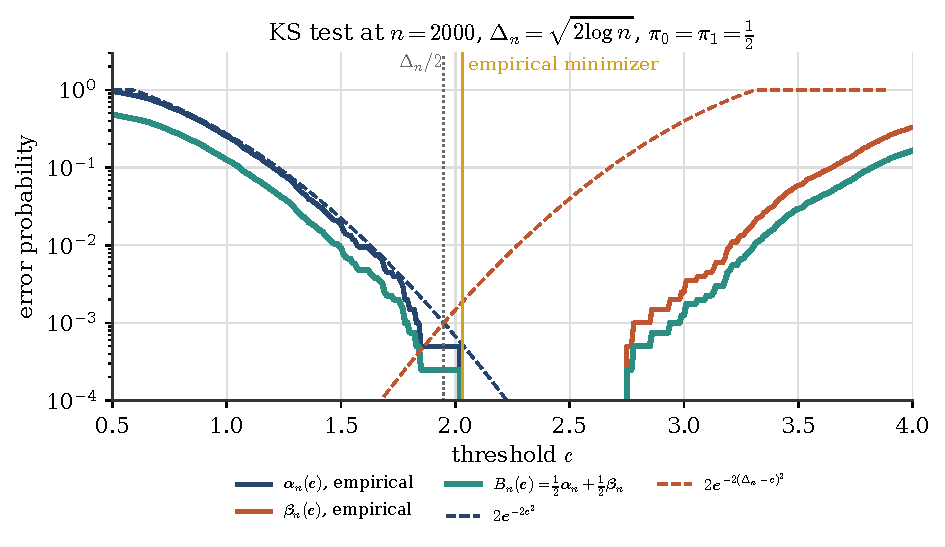
\includegraphics[width=0.78\textwidth]{rs_bayes_balance}
\caption{Type I error $\alpha_n(c)$, Type II error $\beta_n(c)$, and Bayes risk $B_n(c) = \tfrac{1}{2}\alpha_n + \tfrac{1}{2}\beta_n$ for the KS testing problem of Section~\ref{np:sec:rs-setup} at $n = 2000$, with Pitman shift alternative at the detectability boundary $\Delta_n = \sqrt{2\log n}$. Empirical curves (solid) from $2000$ Monte Carlo replications under each hypothesis, with the asymptotics (dashed): the empirical $\alpha_n$ tracks the Kolmogorov tail $2e^{-2c^2}$, while the empirical $\beta_n$ lies far below the Pitman-shifted tail $2e^{-2(\Delta_n - c)^2}$, which the Type~II analysis gives only as an upper bound. The empirical Bayes risk vanishes between the largest null and the smallest alternative statistic, so its minimizer, $2.03$, sits just above the largest null statistic and does not resolve the balanced threshold $c_n^* = \Delta_n/2 \approx 1.95$.}
\label{np:fig:rs-bayes}
\end{figure}

\subsubsection{Bridge to the predictive setting}\label{np:sec:rs-bridge}

Theorem~\ref{np:thm:rs} is the testing-side ancestor of the KS-truncated predictive density of Section~\ref{np:sec:ks}. The structural correspondence is: the rejection threshold $c$ in testing plays the role of the truncation level $a$ in prediction, both calibrated against the empirical-process tail $\sup_x|G_n(x)|$ at the moderate-deviation scale.

The numerical scale differs by a factor of $2$ between the two settings. In testing, balancing $\pi_0\alpha$ against $\pi_1\beta$ with $\pi_0 = \pi_1$ gives $c_n^* = \Delta_n/2$ at the boundary of detectability. In prediction, with $\Delta_n$ now the KS distance between $P_0$ and $\Pi^*P_0$, the trade-off is between empirical variance (which grows with $a$) and truncation bias (which decays exponentially in $a$ once $a$ exceeds $\Delta_n$); Conjecture~\ref{np:conj:ks-mdp} puts $a_n^* = \Delta_n(1+o(1))$, twice $c_n^*$ on the same bridge scale, and so $a_n^* = \sqrt{2\log n}\,(1+o(1))$ at the boundary $\Delta_n = \sqrt{2\log n}$. Both are instances of the same Rubin--Sethuraman risk-balancing principle, applied to different loss functions.

\medskip
\noindent\emph{General Rubin--Sethuraman lemma.} The KS-specific Theorem~\ref{np:thm:rs} extends, on the logarithmic scale, to any test statistic $T_n$ with moderate-deviation tails under the null and under alternatives at a detection scale; Datta, Polson, Sokolov and Zantedeschi (2026) calibrate parametric tests on the same scale.

\begin{theorem}[Rubin--Sethuraman risk-balancing, general form]\label{np:thm:rs-general}
Let $T_n$ satisfy $T_n/\sigma_n \toL Z$ with non-degenerate limit, and let the alternatives sit at detection scale $\Delta_n \to \infty$, with moderate-deviation tails $\PP_0(T_n > a\sigma_n) = e^{-a^2/2 + o(\Delta_n^2)}$ and $\PP_1(T_n \le a\sigma_n) = e^{-(\Delta_n - a)^2/2 + o(\Delta_n^2)}$ uniformly in $0 < a < \Delta_n$. For the Bayes risk $\mathcal{R}_n(a) = \pi_0\PP_0(T_n > a\sigma_n) + \pi_1\PP_1(T_n \le a\sigma_n)$ with $\log(\pi_0/\pi_1)/\Delta_n^2 \to \lambda \in (-\tfrac12, \tfrac12)$, every Bayes-risk-minimizing threshold satisfies
\[
a_n^* \;=\; \Bigl(\frac{\Delta_n}{2} + \frac{\log(\pi_0/\pi_1)}{\Delta_n}\Bigr)(1+o(1)), \qquad \mathcal{R}_n(a_n^*) \;=\; \pi_0\,e^{-(a_n^*)^2/2 + o(\Delta_n^2)}.
\]
When the prior odds $\pi_0/\pi_1 = b_n \ge 1$ count $b_n$ competing hypotheses (the reciprocal of the odds $b_n = \pi_1/\pi_0$ of Theorem~\ref{np:thm:rs}), $a_n^* \ge \sqrt{2\log b_n}\,(1+o(1))$, so the multiple-comparison scale $\sqrt{2\log b_n}$ is a lower bound for the threshold, and $\mathcal{R}_n(a_n^*) \le \pi_1 < b_n^{-1}$.
\end{theorem}

\begin{proof}
For $0 < a < \Delta_n$, $\log\mathcal{R}_n(a) = \max\{\log\pi_0 - a^2/2,\ \log\pi_1 - (\Delta_n - a)^2/2\} + o(\Delta_n^2)$. The first term decreases and the second increases in $a$; they cross at $a = \Delta_n/2 + \log(\pi_0/\pi_1)/\Delta_n$, where both slopes are of order $\Delta_n$, so a minimizer lies within $o(\Delta_n)$ of the crossing, and thresholds outside $(0,\Delta_n)$ do worse because the two error probabilities are monotone in $a$. The lower bound is the arithmetic--geometric mean inequality $\Delta_n/2 + \log b_n/\Delta_n \ge \sqrt{2\log b_n}$, and $\mathcal{R}_n(a_n^*) \le \lim_{a\to\infty}\mathcal{R}_n(a) = \pi_1$.
\end{proof}

Theorem~\ref{np:thm:rs} is the KS instance of Theorem~\ref{np:thm:rs-general}, sharpened to factors $1+o(1)$: with $\sigma_n = 1/2$ the Kolmogorov tail $2e^{-2c^2}$ is $2e^{-a^2/2}$ at $a = 2c$, the detection scale doubles to $2\Delta_n$, and $\pi_0/\pi_1 = b_n^{-1}$, so $c_n^* = a_n^*/2 = (\Delta_n/2 - \log b_n/(4\Delta_n))(1+o(1))$, which is $\tfrac12\Delta_n(1+o(1))$ in the interior regime and $\tfrac38\Delta_n(1+o(1))$ at $b_n = n$. For nonparametric Bayes prediction (Section~\ref{np:sec:master}), the $b_n = \pi_0/\pi_1$ of Theorem~\ref{np:thm:rs-general} is the cardinality of an adaptive grid over an unknown structural parameter (bandwidth, smoothness, truncation level). A grid of polynomial size has $\log b_n \asymp \log n$, but the bandwidth and level grids of Section~\ref{np:sec:apps} have $b_n$ of order $\log n$, so $\log b_n$ is of order $\log\log n$ there.

\subsection{Predictive Bayes Risk via Fubini}\label{np:sec:ks}

We now show that the Rubin--Sethuraman risk-balancing argument of Section~\ref{np:sec:rs} transfers from the testing setting to the predictive setting through a Fubini factorization of the predictive Bayes risk. The empirical CDF $F_n$, used in Section~\ref{np:sec:rs} as a sufficient summary for the KS test statistic, also serves as the natural conditioning statistic for the predictive distribution\index{predictive distribution} under any prior that admits a closed-form posterior on $F$ as a function of $F_n$.

\subsubsection{Fubini factorization}\label{np:sec:fubini}

For any prior $\Pi$ on CDFs with proper posterior $\Pi(\cdot \mid X^{(n)})$, the predictive density is the posterior mean,
\begin{equation}\label{np:eq:pred-density}
\hat p_\Pi(y \mid X^{(n)}) \;=\; \int f(y)\,\Pi(dF \mid X^{(n)}),
\end{equation}
and the predictive Bayes risk admits the Fubini factorization
\begin{equation}\label{np:eq:fubini-risk}
R_{\KL}(P_0;\hat p_\Pi)
\;=\; \E_{X^{(n)}\sim P_0^{\otimes n}}\!\int p_0(y)\,\log\!\frac{p_0(y)}{\int f(y)\,\Pi(dF\mid X^{(n)})}\,dy.
\end{equation}
The integrand is a function of $X^{(n)}$ only through the conditioning of $\Pi$ on the data; when the prior admits a sufficient statistic for the data (as is the case for the Dirichlet process and Pólya tree priors), the conditioning collapses to a function of $F_n$.

\begin{remark}[Sufficiency of $F_n$]\label{np:rem:sufficiency}
For the Dirichlet process $\Pi = \mathrm{DP}(\alpha_0, F_0)$, the empirical CDF $F_n$ is a sufficient statistic for $F$: the posterior depends on the data only through $(n, F_n)$, with
\begin{equation}\label{np:eq:dp-posterior}
F \mid X^{(n)} \;\sim\; \mathrm{DP}\!\left(\alpha_0 + n,\; \frac{\alpha_0 F_0 + n F_n}{\alpha_0 + n}\right).
\end{equation}
This is Ferguson's (1973) fundamental conjugacy. An analogous sufficiency holds for the canonical P\'olya tree, with the dyadic cell counts of $F_n$ playing the role of the sufficient statistic.
\end{remark}

\subsubsection{Connection to Carota--Parmigiani Bayes factors}\label{np:sec:cp}

A direct precedent for the Fubini factorization \eqref{np:eq:fubini-risk} is the Bayes-factor literature on Bayesian nonparametric goodness-of-fit testing initiated by Carota and Parmigiani (1996) and developed in Carota, Parmigiani, and Polson (1996). We summarize here the relevant elements: the testing model, the resulting Bayes factor, and the inconsistency phenomenon, and we explain how each plays out in our predictive setting.

\paragraph{The model: parametric null vs.\ Dirichlet-process alternative}\label{np:sec:cp-model}

Carota and Parmigiani (1996) consider the goodness-of-fit testing problem
\begin{equation}\label{np:eq:cp-hypotheses}
H_0:\ F = F_0 \qquad \text{vs.} \qquad H_1:\ F \sim \Pi = \mathrm{DP}(\alpha_0, F_0),
\end{equation}
where $F_0$ is a fixed parametric null CDF, $\alpha_0 > 0$ is a prior concentration parameter, and $\Pi$ is a Dirichlet process centered at $F_0$. The alternative is a \emph{nonparametric elaboration} of the null: $\Pi$ is centered at $F_0$ and its spread about $F_0$ is controlled by $\alpha_0$, with $\alpha_0 \to \infty$ collapsing $\Pi$ onto the point mass at $F_0$ and $\alpha_0 \to 0$ collapsing it onto the law of a single atom $\delta_X$ with $X \sim F_0$, since the first stick-breaking weight, a $\mathrm{Beta}(1,\alpha_0)$ variable, tends to $1$: the limit is degenerate, not weakly informative. The model is the canonical Bayesian counterpart to the frequentist goodness-of-fit problem, with the Dirichlet process serving as the natural nonparametric alternative (Ferguson, 1973; Lo, 1984).

The Carota--Parmigiani--Polson (1996) ``model elaboration'' framework places the testing problem in the broader context of Bayesian model criticism: the elaboration $H_1$ extends $H_0$ in a controlled nonparametric direction, and the diagnostic value of the elaboration is measured by the KL divergence between the marginal prior and posterior on the elaboration parameter $F$.

\paragraph{The Bayes factor}\label{np:sec:cp-bayes-factor}

Under the model \eqref{np:eq:cp-hypotheses}, the Bayes factor in favor of $H_1$ is the marginal-likelihood ratio
\begin{equation}\label{np:eq:cp-bf}
BF_{10} \;=\; \frac{m_1(X^{(n)})}{m_0(X^{(n)})} \;=\; \frac{\int \prod_{i=1}^n f(X_i)\,\Pi(dF)}{\prod_{i=1}^n f_0(X_i)},
\end{equation}
computed by Fubini as an integral of the data likelihood against the prior on $F$. For the Dirichlet-process alternative, the P\'olya urn predictive collapses $m_1$ to a function of the partition structure of $X^{(n)}$ (Blackwell and MacQueen, 1973): writing $K_n$ for the number of distinct values in $X^{(n)}$ and $n_1,\dots,n_{K_n}$ for their multiplicities,
\begin{equation}\label{np:eq:cp-marg-lik}
m_1(X^{(n)}) \;=\; \frac{\alpha_0^{K_n}\,\prod_{j=1}^{K_n}(n_j - 1)!}{\alpha_0(\alpha_0+1)\cdots(\alpha_0+n-1)} \cdot \prod_{j=1}^{K_n}f_0(x_j^*),
\end{equation}
where $x_1^*,\dots,x_{K_n}^*$ are the distinct values. For continuous data and continuous $f_0$, all observations are almost surely distinct ($K_n = n$), and the Bayes factor reduces to a function of $n$ and $\alpha_0$ alone, demonstrating the well-known Carota--Parmigiani inconsistency described below. For discrete data or for the canonical P\'olya tree alternative (Lavine, 1992), the marginal likelihood reduces to a function of the dyadic-cell counts of $F_n$, an explicit summary statistic. Both constructions illustrate the same Fubini sufficiency principle as our predictive density \eqref{np:eq:pred-density}: the Bayes-optimal summary is the empirical CDF (or its sufficient sub-statistic), and risks are functionals of it.

\paragraph{Carota--Parmigiani inconsistency and the Sanov-floor analogy}\label{np:sec:cp-results}

The principal finding of Carota and Parmigiani (1996) is that for continuous data, the Bayes factor \eqref{np:eq:cp-bf} is \emph{inconsistent under the alternative}: even when the data are generated from a $P_0 \ne F_0$, the Bayes factor does not diverge to $+\infty$ in general. The reason is structural: the Dirichlet process places all its mass on discrete distributions, so for continuous $P_0$ the marginal likelihood ratio under $H_1$ is the data-free constant $\alpha_0^n/\{\alpha_0(\alpha_0+1)\cdots(\alpha_0+n-1)\}$, which tends to zero whatever $P_0$ is. This inconsistency under continuous alternatives is well known in the Bayesian nonparametric literature (Tokdar and Martin, 2021); the Carota--Parmigiani (1996) contribution was to characterize it and to propose remedies via mixture priors and pseudo-Bayes-factor calibrations.

The Carota--Parmigiani inconsistency is the testing-side analogue of the \emph{Sanov-floor phenomenon} of our Theorem~\ref{np:thm:abc-csiszar}, misspecified case. Both arise from the same mechanism: a prior $\Pi$ whose Kullback--Leibler support $\supp(\Pi)$ does not contain the data-generating measure $P_0$. In testing: the Bayes factor cannot tell apart $H_0$ from a $P_0 \notin \supp(\Pi)$, because $P_0$ is invisible to $\Pi$. In prediction: the predictive risk has an irreducible floor $\KL(P_0\|\Pi^*P_0) > 0$, because the predictive density is constrained to $\supp(\Pi)$ and cannot reach $P_0$. In both cases the diagnostic is the reverse I-projection: knowing $\Pi^*P_0$ tells us where the prior ``thinks'' the truth lies, and the distance $\KL(P_0\|\Pi^*P_0)$ measures the unavoidable cost of the misspecification.

The remedy in both settings is also the same: enrich the prior to include a population-level neighborhood of $P_0$. For testing, the Carota--Parmigiani (1996) mixture-prior construction and the Verdinelli--Wasserman (1998) infinite-dimensional exponential family achieve this. For prediction, the Dirichlet-process mixture of Gaussians, with a bandwidth prior that charges every neighborhood of $0$, and the canonical P\'olya tree have every density satisfying Assumption~\ref{np:ass:density} in their Kullback--Leibler support (Examples~\ref{np:ex:dp-iproj} and \ref{np:ex:pt-iproj}), which eliminates the Sanov floor at the population level.

\subsubsection{The KS-truncated predictive density}\label{np:sec:ks-truncation}

We now turn to a specific summary-posterior construction motivated by the KS statistic: clip the empirical CDF to a moderate-deviation envelope of the reverse I-projection $F_\Pi^*$.

\begin{definition}[KS-truncated predictive CDF]\label{np:def:ks-pred}
For truncation level $a > 0$,
\begin{equation}\label{np:eq:ks-trunc}
\widehat{F}^{(a)}_n(x) \;:=\; F_\Pi^*(x) + \clip\!\left(F_n(x) - F_\Pi^*(x),\,-\tfrac{a}{\sqrt{n}},\,+\tfrac{a}{\sqrt{n}}\right),
\end{equation}
with $\clip(u,-t,t) := \max(-t,\min(t,u))$. The associated predictive density $\widehat{p}^{(a)}_n$ is obtained by differentiation followed by kernel smoothing of bandwidth $h_n\to 0$.
\end{definition}

\begin{remark}[KS-truncation as a posterior mode]\label{np:rem:ss-prior}
The estimator \eqref{np:eq:ks-trunc} is not a spike-and-slab posterior. Under a spike-and-slab prior on the increments of $F - F_\Pi^*$ (at each dyadic cell $B$, an atom at $0$ with probability $p_0$ and a diffuse component with probability $1-p_0$), the posterior thresholds the empirical increment $F_n(B) - F_\Pi^*(B)$ at a level determined by $(p_0, n)$: it sets small increments to zero and keeps large ones, whereas \eqref{np:eq:ks-trunc} keeps small deviations and caps large ones at $\pm a/\sqrt{n}$. The clip is a pointwise posterior mode: approximate the likelihood of $F_n(x)$ by a normal density with mean $F(x)$ and fixed variance, and give $F(x) - F_\Pi^*(x)$ a flat prior on $[-a/\sqrt{n}, a/\sqrt{n}]$; the posterior is that normal density, with mean $F_n(x) - F_\Pi^*(x)$, restricted to the interval, and its mode is the point of the interval nearest that mean. The Dirichlet-process posterior \eqref{np:eq:dp-posterior} is the linear-shrinkage analogue, obtained from a single-component diffuse prior with no atom at zero.
\end{remark}

\subsubsection{Bayes-risk-optimal truncation}

\begin{conjecture}[Optimal truncation at the moderate-deviation scale]\label{np:conj:ks-mdp}
Under Assumptions~\ref{np:ass:density}--\ref{np:ass:wongshen}, let $P_0$, which may depend on $n$, have CDF $F_{P_0}$, and let $\Delta_n := \sqrt{n}\sup_x|F_{P_0}(x) - F_\Pi^*(x)|$, the detection distance of Section~\ref{np:sec:rs-setup} with $P_0$ and $\Pi^*P_0$ in place of the alternative and the null. If $\Delta_n \to \infty$ and $h_n\Delta_n^2 \to \infty$, the Bayes-risk-optimal truncation level for the predictive density associated with \eqref{np:eq:ks-trunc} satisfies $a_n^* = \Delta_n(1+o(1))$. In particular, at the detection boundary $\Delta_n = \sqrt{2\log n}$, with $h_n\log n \to \infty$,
\begin{equation}\label{np:eq:a-star}
a_n^* \;=\; \sqrt{2\log n}\,(1+o(1)).
\end{equation}
\end{conjecture}

\noindent\textbf{Heuristic.}
The empirical process\index{empirical process theory} $G_n(x) := \sqrt{n}(F_n(x) - F_\Pi^*(x))$ converges weakly under $P_0 = \Pi^*P_0$ to a Brownian bridge composed with $F_\Pi^*$. The truncation-active event $\mathcal{A}_n(a) := \{\sup_x|G_n(x)| > a\}$ has Kolmogorov-tail probability
\[
\PP_0\bigl(\mathcal{A}_n(a)\bigr) \;\le\; 2\,e^{-2a^2}\,(1+o(1))
\]
by Smirnov (1944). The expected KL contribution decomposes as
\[
J_n^{(a)} \;\approx\; \underbrace{v_n(a)}_{\text{empirical variance on }\mathcal{A}_n(a)^c} \;+\; \underbrace{\mathrm{bias}_n(a)\cdot \PP_0\bigl(\mathcal{A}_n(a)\bigr)}_{\text{truncation bias on }\mathcal{A}_n(a)},
\]
where $v_n(a) = O((nh_n)^{-1})$ from kernel smoothing and $\mathrm{bias}_n(a)$ is the per-active-instance bias, bounded above by a constant for bounded densities. For $P_0=\Pi^*P_0$ there is nothing to balance: truncation pulls $F_n$ toward the CDF of $P_0$ itself, so it adds no bias, and $a = 0$, which returns that CDF, is best. A truncation bias needs $P_0 \ne \Pi^*P_0$. Then $G_n$ is the signal $\sqrt{n}(F_{P_0} - F_\Pi^*)$, of height $\Delta_n$, plus a noise whose supremum exceeds $t$ with probability at most $2e^{-2t^2}$. A level $a \le (1-\delta)\Delta_n$ clips the signal on an interval and adds a bias of order $\Delta_n^2/n$ to the predictive risk, more than the variance $O((nh_n)^{-1})$ that clipping saves once $h_n\Delta_n^2 \to \infty$, while a level $a \ge (1+\delta)\Delta_n$ is active with probability at most $2e^{-2\delta^2\Delta_n^2}$ and acts almost as $a = \infty$. Hence $a_n^* = \Delta_n(1+o(1))$, and at $a_n^*$ the risk is, to first order, that of the untruncated estimate. A fixed $P_0 \ne \Pi^*P_0$ has $\Delta_n$ of order $\sqrt{n}$ (in the Monte Carlo below, $\Delta_n = \sqrt{2n}/(4\pi) \approx 0.113\sqrt{n}$), so the moderate-deviation level $\sqrt{2\log n}$ arises only at the detection boundary.

\medskip
A rigorous proof requires KMT-type strong approximation of $F_n - F_\Pi^*$ together with uniform-in-$a$ control of the truncation bias under both well- and misspecified regimes; we leave this for separate work and give a numerical check here.

\subsubsection{Monte Carlo verification}\label{np:sec:ks-mc}

Take $\X = [0,1]$, true density $p_0(x) = 1 + 0.5\sqrt{2}\cos(2\pi x)$, baseline $F_\Pi^*(x) = x$. For each $n$, draw $n$ samples from $p_0$, form $F_n$, evaluate \eqref{np:eq:ks-trunc} on a grid of $a$, differentiate with Gaussian smoothing, and compute $\KL(p_0\|\widehat p^{(a)}_n)$ by numerical integration. For each $a$ the KL risk is averaged over 15 replications, the same samples serving every $a$, and $\hat a_n^*$ is its minimizer over 65 equally spaced values of $a$ in $[0.5,12.5]$, a grid that runs past the KS distance $\Delta_n = \sqrt{2n}/(4\pi)$ between $P_0$ and the baseline at every $n$:

\begin{center}
\begin{tabular}{@{}rrrrr@{}}
\toprule
$n$ & $\hat a_n^*$ (MC) & $\Delta_n$ & $\hat a_n^*/\Delta_n$ & $\sqrt{2\log n}$ \\
\midrule
$100$ & $0.50$ & $1.13$ & $0.44$ & $3.03$ \\
$200$ & $0.50$ & $1.59$ & $0.31$ & $3.26$ \\
$500$ & $2.38$ & $2.52$ & $0.94$ & $3.53$ \\
$1000$ & $3.50$ & $3.56$ & $0.98$ & $3.72$ \\
$2000$ & $5.56$ & $5.03$ & $1.11$ & $3.90$ \\
$5000$ & $8.75$ & $7.96$ & $1.10$ & $4.13$ \\
\bottomrule
\end{tabular}
\end{center}

\smallskip
For $n \ge 500$ the minimizer follows $\Delta_n$, with $\hat a_n^*/\Delta_n$ between $0.94$ and $1.11$, consistent with Conjecture~\ref{np:conj:ks-mdp}, and it parts from $\sqrt{2\log n}$, which $\Delta_n$ crosses near $n = 1100$: this $P_0$ is fixed, so $\Delta_n$ grows like $\sqrt n$. At $n = 2000$ and $5000$ the minimizer lies just above $\Delta_n$, and its risk is within $2\%$ of the risk at $a = 12.5$, where the clip is inactive, so truncation gains almost nothing at $\hat a_n^*$, as the heuristic predicts. Small-$n$ values are prior-dominated (heavy truncation), with $\hat a_n^*$ at the lower end of the grid. Figure~\ref{np:fig:ks-mdp} plots $\hat a_n^*$ against $\Delta_n$ and $\sqrt{2\log n}$.

\begin{figure}[H]
\centering
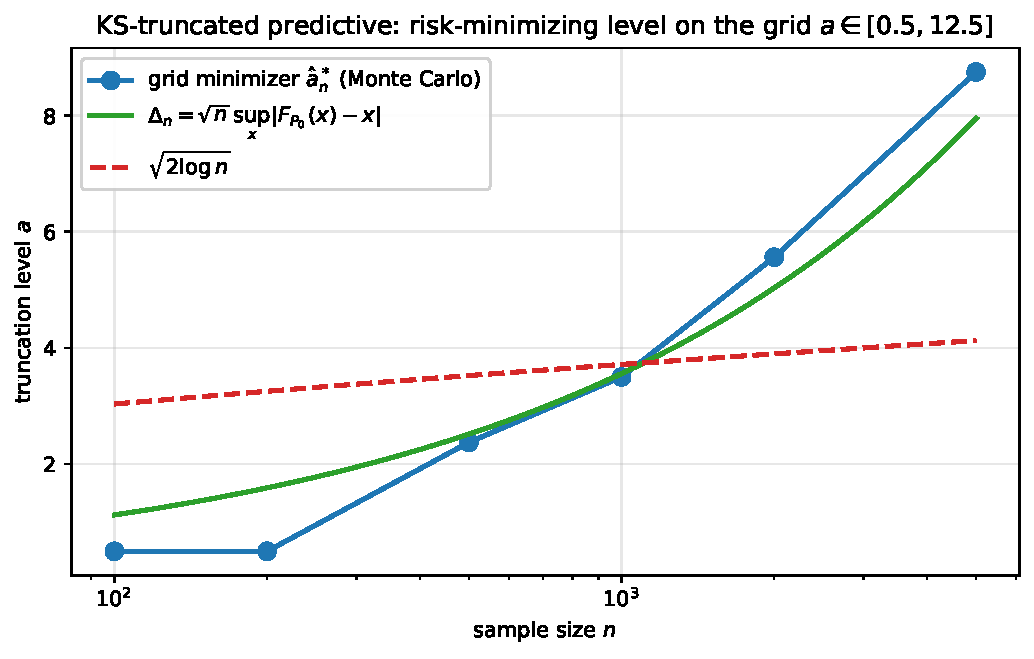
\includegraphics[width=0.72\textwidth]{ks_mdp_scaling}
\caption{KS-truncation level $\hat a_n^*$ minimizing the Monte Carlo risk over the grid $a\in[0.5,12.5]$, against the KS distance $\Delta_n = \sqrt{2n}/(4\pi)$ of $P_0$ from the baseline and the moderate-deviation scale $\sqrt{2\log n}$.}
\label{np:fig:ks-mdp}
\end{figure}

\subsubsection{Structural parallel}

\begin{center}
\renewcommand{\arraystretch}{1.15}
\begin{tabular}{@{}lll@{}}
\toprule
& \textbf{KS testing} (arXiv:2602.15297) & \textbf{KS-truncated prediction} \\
\midrule
Loss & $0/1$ & $\KL(p_0\|\hat p)$ \\
Object & $T_n = \sqrt{n}\sup|F_n - F_0|$ & $\widehat F^{(a)}_n$ from \eqref{np:eq:ks-trunc} \\
Calibration scale & $c_n^* = \tfrac12\sqrt{2\log n}$ & $a_n^* = \sqrt{2\log n}$ (conjectured) \\
Minimum risk & $O(1/n)$ & as at $a = \infty$ (heuristic) \\
Driver & Kolmogorov tail of $\sup|B^\circ|$ & Same \\
\bottomrule
\end{tabular}
\end{center}

\medskip
\noindent\textbf{Unifying observation.} The empirical CDF $F_n$ is the nonparametric Bayes counterpart of the marginal-likelihood score $\nabla\log m_n$ in the parametric horseshoe\index{horseshoe prior} paper (Polson, Sokolov and Zantedeschi, 2026c, arXiv:2604.01266): both are the natural data-summary statistics on which Bayes-optimal calibration operates, and at the detection boundary both produce the canonical $\sqrt{2\log n}$ scale via moderate-deviation Bayes-risk balancing.

\subsection{Master Decomposition}\label{np:sec:master}

\begin{theorem}[Master decomposition]\label{np:thm:master}
Under Assumptions~\ref{np:ass:density}--\ref{np:ass:wongshen}, the decomposition of Theorem~\ref{np:thm:abc-csiszar} holds. Let $U_n := \{P : \dH(P,\Pi^*P_0) \le M\eps_n,\ \pi^* \le M_{\rm WS}\,p\}$, with $M$ and the Hellinger contraction rate $\eps_n$ of Assumption~\ref{np:ass:contraction} and $M_{\rm WS}$ of Assumption~\ref{np:ass:wongshen}. If $\E_{P_0^{\otimes n}}\int_{U_n^c}\KL(\pi^*\|p)\,\Pi(dP \mid X^{(n)}) = O(\eps_n^2)$, then
\begin{equation}\label{np:eq:master-rate}
J_n(\Pi,P_0) \;=\; O(\eps_n^2).
\end{equation}
For a prior that adapts over a grid of size $b_n$, $\eps_n$ is the contraction rate of the adaptive posterior, which may carry polylog factors.
\end{theorem}

\begin{proof}
The decomposition is Theorem~\ref{np:thm:abc-csiszar}, and its dichotomy follows once $J_n\to0$. Wong--Shen converts Hellinger contraction at rate $\eps_n$ into KL contraction at $\eps_n^2$: since $q \mapsto \KL(\pi^*\|q)$ is convex, $\KL(\pi^*\|\hat p_\Pi) \le \int \KL(\pi^*\|p)\,\Pi(dP \mid X^{(n)})$; once $M\eps_n \le \eta$, Assumption~\ref{np:ass:wongshen} bounds the integrand by $C_{\rm WS}M^2\eps_n^2$ on $U_n$, and the hypothesis bounds the expected integral over $U_n^c$ by $O(\eps_n^2)$.
\end{proof}

\begin{remark}[Price of adaptation, heuristic]\label{np:rem:adaptive}
For a prior that adapts over a grid of size $b_n$ (the adaptation grid cardinality), the following heuristic, which we do not prove, suggests a price of adaptation of order $(\log b_n)^{\kappa}$ for some $\kappa > 0$, beyond the squared rate at the best grid point. The marginal-likelihood selector would concentrate within $O(\sqrt{\log b_n})$ of the optimal structural parameter, as the multiple-comparison scale $\sqrt{2\log b_n}$ of Theorem~\ref{np:thm:rs-general} suggests, and a second-order Taylor expansion of $\eps_n^2(\cdot)$ around its optimum would then produce $(\log b_n)^{\kappa}$. For the bandwidth and level grids of Section~\ref{np:sec:apps}, $b_n$ is of order $\log n$, so this price is a power of $\log\log n$, within the $(\log n)^{\kappa(\Pi)}$ factors of Table~\ref{np:tab:kappas}.
\end{remark}

\begin{table}[h]
\centering
\renewcommand{\arraystretch}{1.15}
\begin{tabular}{@{}lll@{}}
\toprule
\textbf{Prior} & $\kappa(\Pi)$ & \textbf{Adaptive grid} \\
\midrule
DPM of Gaussians & $1$ & bandwidth $h \in [n^{-1/(2B+1)},\,1]$ \\
Canonical P\'olya tree & $1$ & truncation level $L \in [1,\,\log_2 n]$ \\
Logistic-Gaussian process & $\kappa_{\LGP}(\beta)$ bounded & length-scale $A \in [1,\,n^{1/(2\nu+1)}]$ \\
\bottomrule
\end{tabular}
\caption{Adaptive penalty exponents $\kappa(\Pi)$ of the bounds $J_n \lesssim n^{-2\beta/(2\beta+1)}(\log n)^{\kappa(\Pi)}$ in Theorems~\ref{np:thm:dp}--\ref{np:thm:gp}.}
\label{np:tab:kappas}
\end{table}

\subsection{Applications: three adaptive priors}\label{np:sec:apps}

Three standard nonparametric priors instantiate the master rate, each with its own adaptive grid: a
Dirichlet-process mixture of Gaussians, a canonical P\'olya tree, and a logistic-Gaussian process. The
three are worked in parallel below, and each is accompanied by a numerical illustration of its
predictive-risk rate.

\subsubsection{Application I: Dirichlet-Process Mixture of Gaussians}\label{np:sec:dp}

The DPM of Gaussians (Escobar and West, 1995; Ghosal, 1999):
$p(\cdot \mid G, h) = \int \phi_h(\cdot - z)\,dG(z)$, $G \sim \mathrm{DP}(\alpha_0, P_*)$, $h \sim \pi_h$ on $[n^{-1/(2B+1)},1]$.

\begin{theorem}[Adaptive DPM rate]\label{np:thm:dp}
For $p_0 \in \mathcal{H}^\beta(L)$ with $\beta \in (0,B]$ unknown, if the data-driven bandwidth $\hat h_n$ stays within constant factors of $h_n^* = n^{-1/(2\beta+1)}$,
\[
J_n(\DPM, P_0) \;\lesssim\; n^{-2\beta/(2\beta+1)}\,(\log n).
\]
\end{theorem}

\begin{proof}
This is a sketch, and its bandwidth hypothesis is assumed rather than proved: van der Vaart and van Zanten (2009) and Castillo (2017) treat Gaussian process and P\'olya tree priors, not the DPM bandwidth. The KL risk decomposes as $J_n = O(h_n^{2\beta}) + (nh_n)^{-1}(1+\delta_n)$; under the hypothesis, bias and variance at $\hat h_n$ stay within constant factors of their values at $h_n^*$, so the price of adaptation $\delta_n$ is bounded. Theorem~\ref{np:thm:rs-general} does not supply a $\log n$ factor here, since the bandwidth grid has $b_n \asymp \log n$ points and $\log b_n \asymp \log\log n$. Balancing at $h_n^*$ yields the bound.
\end{proof}

\paragraph{Numerical illustration.}\label{np:sec:dp-mc}

We illustrate Theorem~\ref{np:thm:dp} on a Beta$(3,3)$ target on $[0,1]$, which is smooth ($C^\infty$). For each $n \in \{100,\allowbreak 200,\allowbreak 500,\allowbreak 1000,\allowbreak 2000,\allowbreak 5000,\allowbreak 10000,\allowbreak 20000\}$ we sample, fit a Gaussian-kernel approximation of the DPM predictive density with oracle bandwidth $h_n^*$ chosen by grid search over $25$ bandwidths in $[0.03, 0.25]$, and compute the predictive KL risk by numerical integration over a $300$-point evaluation grid. The empirical slope, fitted over $500 \le n \le 20000$, is $-0.456$ (Figure~\ref{np:fig:dpm-rate}), flatter than the slope $-0.541$ of the $\beta = 1$ reference $n^{-2/3}\log n$ over the same range. For every $n \ge 1000$ the selected bandwidth is the smallest on the grid, $h = 0.03$, so the search is truncated there and the fitted slope is not a clean estimate of the rate. The Beta$(3,3)$ density vanishes at $0$ and $1$, so it violates Assumptions~\ref{np:ass:density} and~\ref{np:ass:holder}; this experiment and the two below, on the same target, illustrate the rates rather than test the theorems under their hypotheses.

\begin{figure}[H]
\centering
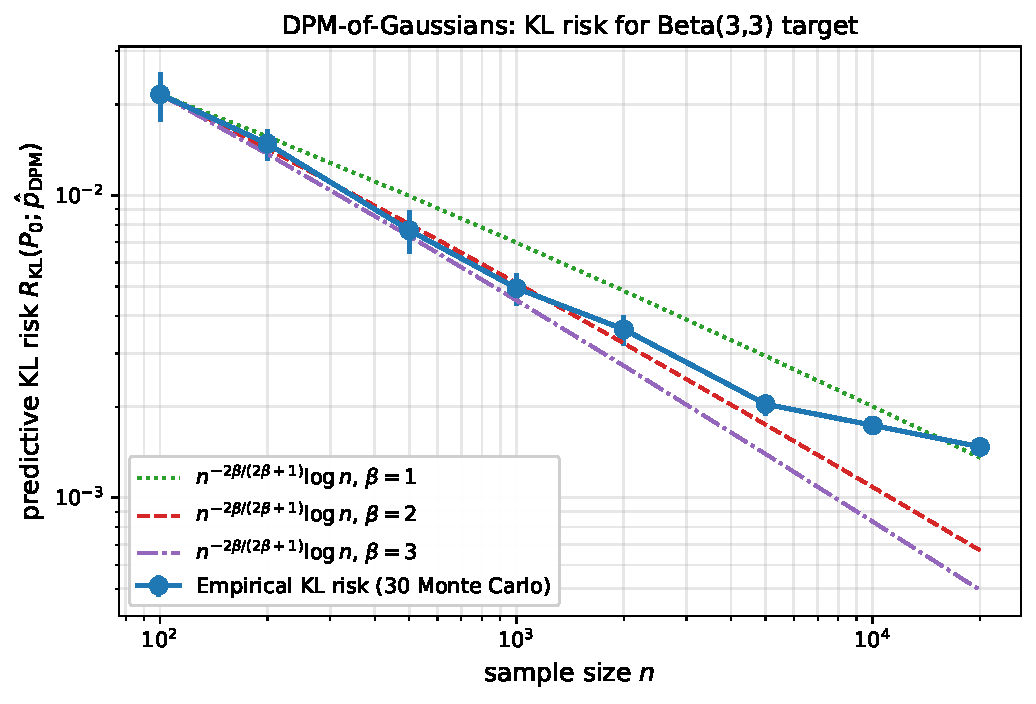
\includegraphics[width=0.72\textwidth]{dpm_rate}
\caption{DPM-of-Gaussians: empirical predictive KL risk against the rate of Theorem~\ref{np:thm:dp}. Beta$(3,3)$ target, 30~Monte Carlo replicates per point, oracle bandwidth.}
\label{np:fig:dpm-rate}
\end{figure}

\subsubsection{Application II: Canonical P\'olya Tree}\label{np:sec:pt}

\begin{theorem}[Adaptive P\'olya tree rate]\label{np:thm:pt}
For $p_0 \in \mathcal{H}^\beta(L)$ with $\beta \in (0,1)$ unknown, if the marginal-likelihood truncation level stays within $O(1)$ of $L_n^* = (\log_2 n)/(2\beta+1)$,
\[
J_n(\PT, P_0) \;\lesssim\; n^{-2\beta/(2\beta+1)}\,(\log n).
\]
\end{theorem}

\begin{proof}
The truncated P\'olya tree at level $L$ has bias $O(2^{-L\beta})$ in $L^2$ (Castillo, 2017, Thm.~2) and variance $O(2^L/n)$. The optimal level is $L_n^* = (\log_2 n)/(2\beta+1)$; the hypothesis, assumed rather than proved in this sketch, keeps the marginal-likelihood selector within $O(1)$ of $L_n^*$, where bias and variance stay within constant factors of their values at $L_n^*$, so balancing them yields the bound. Theorem~\ref{np:thm:rs-general} does not supply the $\log n$ factor, since the dyadic-level grid has $b_n = \log_2 n$ points and $\log b_n \asymp \log\log n$.
\end{proof}

\paragraph{Numerical illustration.}\label{np:sec:pt-mc}

We implement a finite-depth P\'olya tree at oracle level $L_n^*$ chosen by grid search, with a symmetric Dirichlet prior on the dyadic cell masses whose parameter $c\,(L_n^*)^2$ matches the canonical $\beta_\eps = c|\eps|^2$ specification at the finest level only. The Beta$(3,3)$ target is the same as in Section~\ref{np:sec:dp-mc}. The empirical asymptotic slope, fitted over $1000 \le n \le 20000$, is $-0.638$, close to $-2/3$, the power of $n$ in the predicted rate for $\beta = 1$ (Figure~\ref{np:fig:pt-rate}). The dyadic piecewise-constant approximation enforces an effective smoothness of $\beta = 1$, at the boundary of the Hellinger contraction range $\beta \in (0,1)$ for the canonical P\'olya tree (Castillo, 2017, Theorem~2).

\begin{figure}[H]
\centering
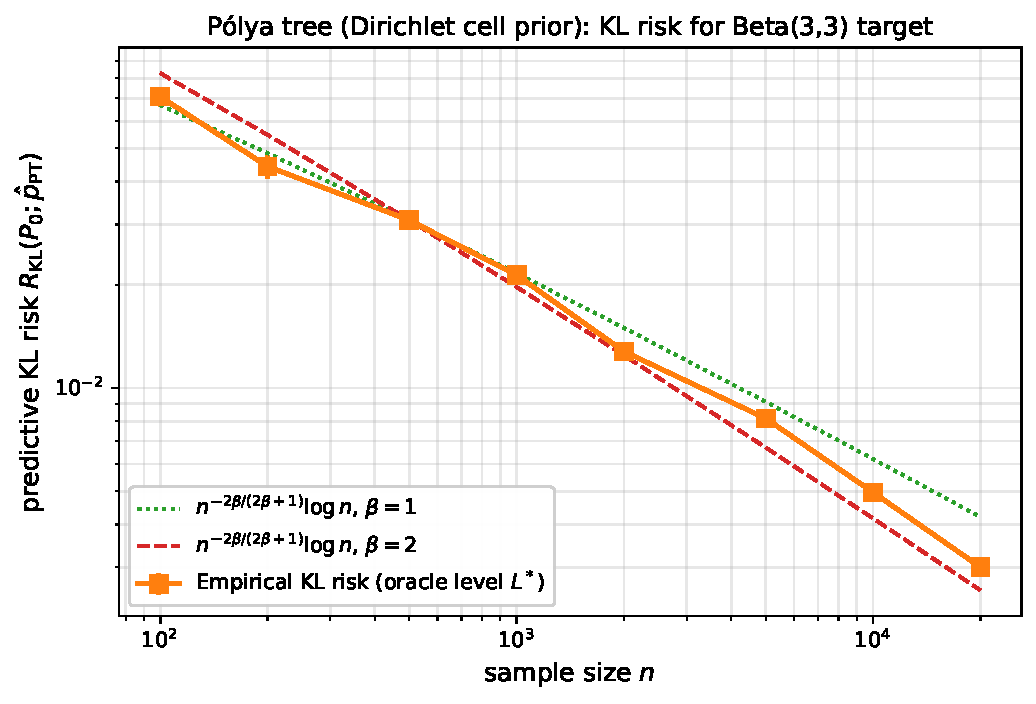
\includegraphics[width=0.72\textwidth]{pt_rate}
\caption{P\'olya tree: empirical predictive KL risk against the rate of Theorem~\ref{np:thm:pt}. Beta$(3,3)$ target, symmetric Dirichlet prior on the cells at the oracle truncation level $L_n^*$, 30~Monte Carlo replicates.}
\label{np:fig:pt-rate}
\end{figure}

\subsubsection{Application III: Logistic-Gaussian Process}\label{np:sec:gp}

Logistic-GP with rescaled Mat\'ern kernel $K_A(x,y) = K(A^{-1}(x-y))$, $K$ Mat\'ern-$\nu$, and length-scale hyperprior on $[1, n^{1/(2\nu+1)}]$.

\begin{theorem}[Adaptive LGP rate]\label{np:thm:gp}
For $p_0 \in \mathcal{H}^\beta(L)$ with $\beta \in (0,B]$ unknown and $\nu \ge B$,
\[
J_n(\LGP, P_0) \;\lesssim\; n^{-2\beta/(2\beta+1)}\,(\log n)^{\kappa_{\LGP}(\beta)},
\]
with $\kappa_{\LGP}(\beta) = (4\beta+1)/(2\beta+1)$, twice the polylog exponent of van der Vaart and van Zanten (2009), provided the posterior contracts in Hellinger at the rate that they prove for the squared exponential kernel (see the proof) and the remaining hypotheses of Theorem~\ref{np:thm:master} (Assumptions~\ref{np:ass:density}--\ref{np:ass:wongshen} and its tail condition) hold.
\end{theorem}

\begin{proof}
For the squared exponential process with a gamma prior on its inverse length-scale, van der Vaart and van Zanten (2009, Thm.~3.1) prove that the LGP posterior contracts at rate $\eps_n = n^{-\beta/(2\beta+1)}(\log n)^{(4\beta+1)/(4\beta+2)}$ in Hellinger; for the rescaled Mat\'ern prior above, the hypothesis of the theorem assumes this rate. Theorem~\ref{np:thm:master}, whose remaining hypotheses are assumed, gives $J_n = O(\eps_n^2)$. In van der Vaart and van Zanten (2009) this $\eps_n$ is the rate of a hierarchical prior with a random length-scale, so it already includes the cost of adaptation, and Theorem~\ref{np:thm:rs-general} adds no further log factor: $\eps_n^2 = n^{-2\beta/(2\beta+1)}(\log n)^{\kappa_{\LGP}(\beta)}$.
\end{proof}

\paragraph{Numerical illustration.}\label{np:sec:gp-mc}

We approximate the LGP posterior predictive by penalized maximum likelihood in a cosine basis with Sobolev-$2$ penalty (Mat\'ern-$3/2$ kernel spectral decay, whose RKHS is the Sobolev space $H^2$), tuning the penalty by grid search. The Beta$(3,3)$ target as before. The empirical asymptotic slope, fitted over $200 \le n \le 5000$, is $-0.667$, matching the power $-2/3$ for $\beta = 1$ to three decimals (Figure~\ref{np:fig:lgp-rate}). The data show no sign of the polylog factor $(\log n)^{\kappa_{\LGP}(1)} = (\log n)^{5/3}$, which would flatten the slope over this range to $-0.421$; the penalized fit is a stand-in for the posterior, so this does not test the exponent $\kappa_{\LGP}$.

\begin{figure}[H]
\centering
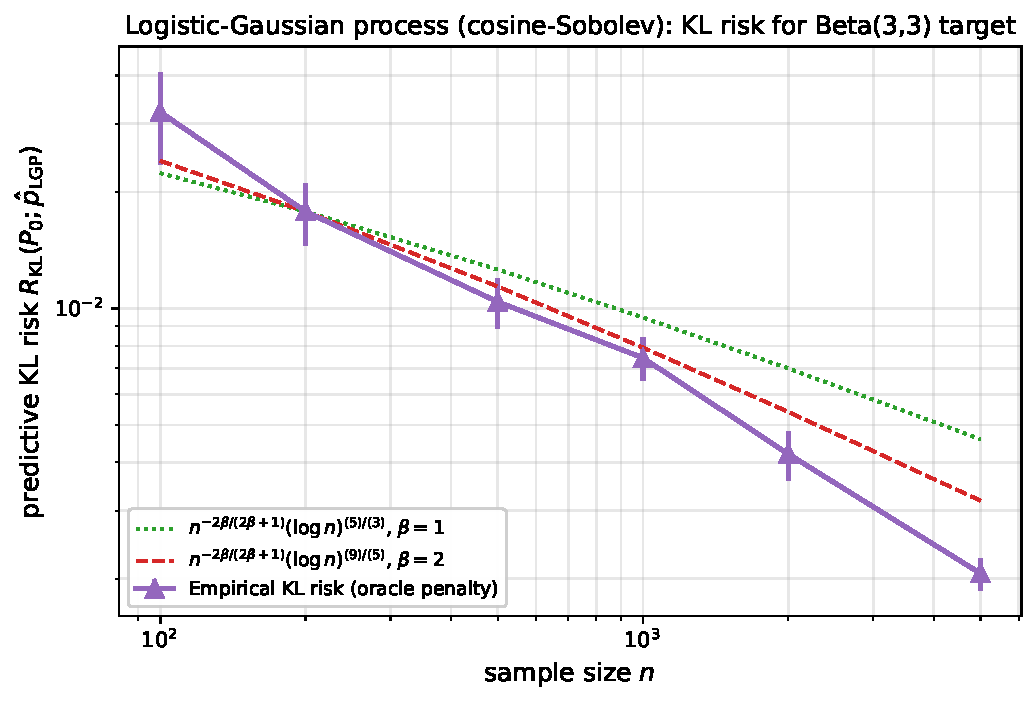
\includegraphics[width=0.72\textwidth]{lgp_rate}
\caption{Logistic-Gaussian process: empirical predictive KL risk against the rate of Theorem~\ref{np:thm:gp}. Cosine basis with Sobolev-$2$ penalty (Mat\'ern-$3/2$), oracle penalty parameter, 20~Monte Carlo replicates per point.}
\label{np:fig:lgp-rate}
\end{figure}

\subsubsection*{Summary across all three priors}\label{np:sec:three-priors-summary}

Figure~\ref{np:fig:combined-priors} overlays the empirical predictive risks of all three priors on the same Beta$(3,3)$ target against the reference $n^{-2/3}\log n$ rate. All three slopes, refitted over the common range $200 \le n \le 5000$ (DPM: $-0.605$, P\'olya tree: $-0.543$, LGP: $-0.667$), lie within $0.13$ of $-2/3$; the DPM and P\'olya tree slopes above are fitted over $500 \le n \le 20000$ and $1000 \le n \le 20000$, hence the difference. Over $200 \le n \le 5000$ the reference $n^{-2/3}\log n$ itself has slope $-0.520$. The three prior architectures thus decay at comparable rates; since the target lies outside the assumptions of Theorem~\ref{np:thm:master}, this illustrates the theorem rather than confirms it.

\begin{figure}[H]
\centering
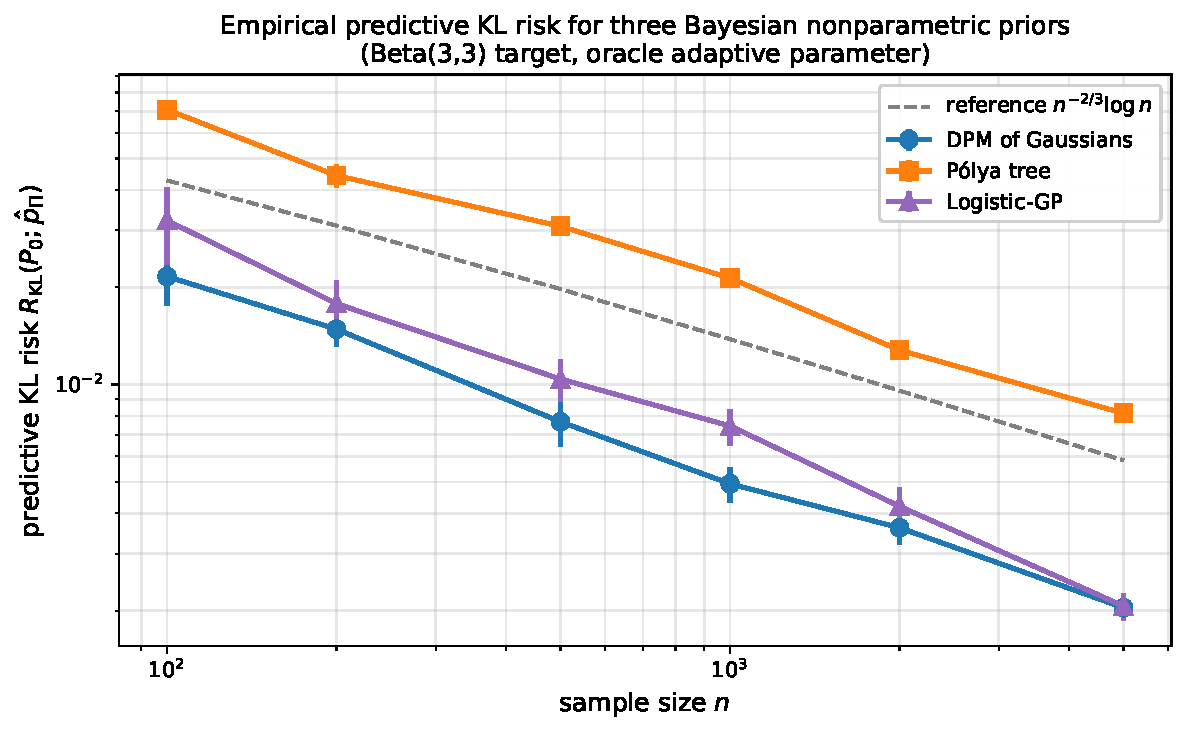
\includegraphics[width=0.78\textwidth]{combined_priors}
\caption{Empirical predictive KL risk for all three Bayesian nonparametric priors on the Beta$(3,3)$ target. All three slopes (DPM, P\'olya tree, LGP), fitted over $200 \le n \le 5000$, lie within $0.13$ of $-2/3$, the power of $n$ in the reference rate $n^{-2/3}\log n$; the LGP slope of $-0.667$ is within $0.001$ of $-2/3$.}
\label{np:fig:combined-priors}
\end{figure}

\subsection{Worked Example: a Sanov Floor in Closed Form}\label{np:sec:miss-example}

We illustrate the decomposition with a misspecified Fourier example admitting closed-form expressions for the Sanov rate, the contraction rate, and the cross term. We then sketch a second example in a Bernoulli-with-calibration setting to demonstrate that the dichotomy is not specific to the Gaussian/cosine geometry.

\subsubsection{Setup}

True density:
\begin{equation}\label{np:eq:ex-truth}
p_0(x) \;=\; 1 + \theta\sqrt{2}\cos(2\pi K_0 x), \qquad x \in [0,1],
\end{equation}
with $\theta \in (0, 1/\sqrt{2})$ and integer $K_0 \ge 3$. The condition $K_0 \ge 3$ ensures $L^2$-orthogonality of $\cos(2\pi K_0 x)$ and $\cos(2\pi x)$ (the prior basis) and avoids the special coupling at $K_0 = 2$ where $\cos(4\pi x) = 2\cos^2(2\pi x) - 1$ would mix the modes. The prior places a uniform law on a one-parameter cosine family at the \emph{wrong} frequency:
\begin{equation}\label{np:eq:ex-prior}
p_a(x) \;=\; 1 + a\sqrt{2}\cos(2\pi x), \qquad a \sim \mathrm{Unif}(-c, c),\ c \in (0, 1/\sqrt{2}).
\end{equation}

\subsubsection{Geometric structure: linear family and Csisz\'ar equality}\label{np:sec:ex-geometry}

The prior support $\{p_a : a \in [-c, c]\}$ is a one-parameter \emph{linear family} in the Csisz\'ar I-divergence sense (Csisz\'ar, 1975): each $p_a$ is a perturbation of the uniform along the single direction $\sqrt{2}\cos(2\pi x)$, orthogonal in $L^2([0,1])$ to the true perturbation $\sqrt{2}\cos(2\pi K_0 x)$. Geometrically, the family is a one-dimensional line through $\pi^* = \mathrm{Unif}$ in the relative-entropy manifold, transverse to the true-direction subspace through $p_0$. The Csisz\'ar Pythagorean equality (Remark~\ref{np:rem:csiszar}) is exact for exponential families, not for this linear family, but it holds here to leading order: the defect $-\int_0^1 (p_0-1)\log p_a\,dx$ involves only the $K_0$-th Fourier coefficient of $\log p_a$, which is $O(a^{K_0})$, so
\begin{equation}\label{np:eq:ex-pythagorean}
\KL(P_0 \| p_a) \;=\; \KL(P_0 \| \mathrm{Unif}) \;+\; \KL(\mathrm{Unif} \| p_a) \;+\; O(\theta a^{K_0}), \quad \forall\, a \in [-c, c].
\end{equation}
The decoupling \eqref{np:eq:ex-pythagorean} is the population-level statement that the Sanov and contraction terms separate to leading order: the first measures the distance from $P_0$ to the prior support transverse to the family, the second measures the distance \emph{within} the family from $\mathrm{Unif} = \pi^*$ to the chosen $p_a$.

\begin{remark}[The cross term is sharper than Cauchy--Schwarz]\label{np:rem:ex-cross}
Theorem~\ref{np:thm:abc-csiszar} bounds the cross term by $C(\sqrt{\KL(P_0\|\Pi^*P_0)\cdot J_n}+J_n)$. The Csisz\'ar equality \eqref{np:eq:ex-pythagorean} shows that the cross term in $R_{\KL}$ is negligible at the population level, up to an $O(\theta a^{K_0})$ correction from the $K_0$-th harmonic of $\log p_a$. The Cauchy--Schwarz bound is therefore loose for this example: at sample size $n$ and fixed $\theta$, the actual remainder is $O(\theta^2/n^{3/2}) = o(1/n)$, coming from third-order Taylor remainder in $\hat a_n$ rather than a structural cross term.
\end{remark}

\begin{figure}[H]
\centering
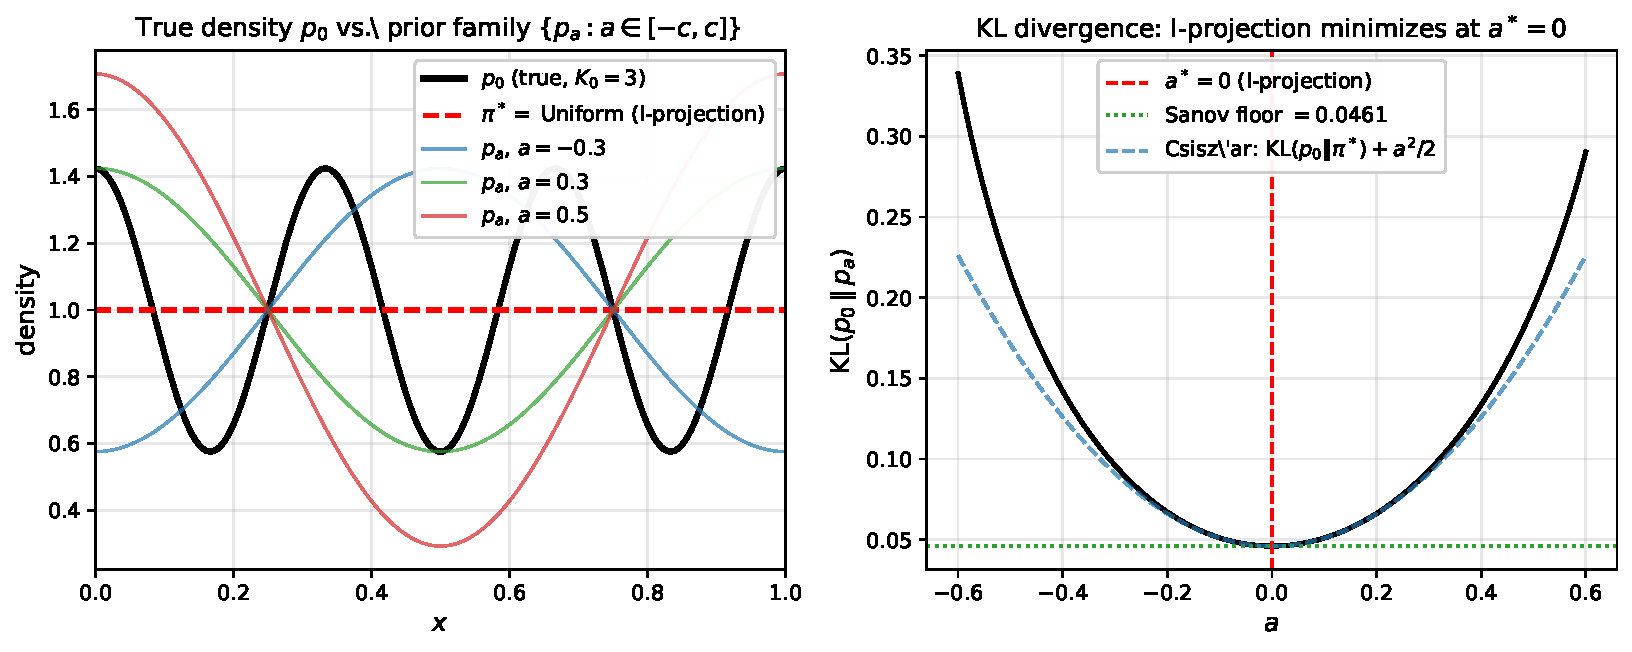
\includegraphics[width=0.95\textwidth]{iproj_geom}
\caption{Reverse I-projection geometry for the worked example. \emph{Left:} the true density $p_0$ (black, $K_0 = 3$ cosine mode) and three priors $p_a$ from the family. The reverse I-projection $\pi^*$ is uniform: any non-uniform $p_a$ adds extra KL by deviating from $\pi^*$. \emph{Right:} the KL parabola in $a$. The horizontal floor at the minimum is the Sanov rate $\KL(P_0\|\pi^*)$; the parabolic excess $a^2/2$ is the Csisz\'ar Pythagorean term $\KL(\pi^*\|p_a)$. Dashed curve: the quadratic approximation $\KL(P_0\|\pi^*) + a^2/2$.}
\label{np:fig:iproj-geom}
\end{figure}

\subsubsection{Closed-form Sanov rate}\label{np:sec:ex-sanov}

\begin{proposition}[Sanov rate, explicit Taylor series]\label{np:prop:ex-iproj}
Under \eqref{np:eq:ex-truth}--\eqref{np:eq:ex-prior} with $K_0 \ge 3$, the reverse I-projection is $\Pi^*P_0 = \mathrm{Unif}([0,1])$, and the Sanov rate is the closed-form series
\begin{equation}\label{np:eq:ex-sanov}
\KL(P_0\|\Pi^*P_0) \;=\; \sum_{k\ge 1}\frac{\binom{2k}{k}}{2^k\,(2k-1)\,(2k)}\,\theta^{2k} \;=\; \frac{\theta^2}{2} + \frac{\theta^4}{8} + \frac{\theta^6}{12} + \frac{5\theta^8}{64} + O(\theta^{10}).
\end{equation}
\end{proposition}

\begin{proof}
The map $a \mapsto \KL(P_0\|p_a) = \int_0^1 p_0\log p_0\,dx - \int_0^1 p_0\log p_a\,dx$ is strictly convex on $[-c,c]$, since $\log p_a(x)$ is concave in $a$, and its derivative at $a = 0$ is $-\sqrt{2}\,\E_{P_0}[\cos(2\pi X)] = 0$ by $L^2$-orthogonality of $\cos(2\pi K_0 x)$ with $\cos(2\pi x)$ for $K_0 \ne 1$, so it is minimized at $a^* = 0$; hence $\Pi^*P_0 = \mathrm{Unif}$ and $\KL(P_0\|\Pi^*P_0) = \int_0^1 p_0\log p_0\,dx$. Writing $u(x) = \theta\sqrt{2}\cos(2\pi K_0 x)$ and expanding $(1+u)\log(1+u) = \sum_{k\ge 1}\bigl((-1)^{k+1}/k\bigr)u^k + \sum_{k\ge 1}\bigl((-1)^{k+1}/k\bigr)u^{k+1}$, the coefficient of $u^{2k}$ in the integrand is $1/[(2k-1)(2k)]$, and odd-power terms vanish upon integration over $[0,1]$ by oddness of cosine integrals. The standard cosine moment $\int_0^1 \cos^{2k}(2\pi K_0 x)\,dx = \binom{2k}{k}/2^{2k}$ gives
\[
\int_0^1 u^{2k}\,dx \;=\; \theta^{2k}\cdot 2^k\cdot \binom{2k}{k}/2^{2k} \;=\; \theta^{2k}\,\binom{2k}{k}/2^k,
\]
and summing yields \eqref{np:eq:ex-sanov}.
\end{proof}

\paragraph{Numerical value of the floor.} At $\theta = 0.3$, the Taylor partial sums are:
\begin{center}
\begin{tabular}{@{}lr@{}}
\toprule
Truncation order & Partial sum\\
\midrule
$\theta^2/2$ & $0.04500$\\
$+\,\theta^4/8$ & $0.04601$\\
$+\,\theta^6/12$ & $0.04607$\\
$+\,5\theta^8/64$ & $0.04608$\\
\midrule
Exact (numerical integration) & $0.04608$\\
\bottomrule
\end{tabular}
\end{center}
The series converges very rapidly for $\theta \le 0.5$, since by Stirling's approximation $\binom{2k}{k} \sim 4^k/\sqrt{\pi k}$, the $k$th coefficient is bounded by $C\,2^k/k^{5/2}$ and the series has radius of convergence $1/2$ in $\theta^2$, i.e., $\theta < 1/\sqrt{2}$.

\subsubsection{Parametric contraction rate}\label{np:sec:ex-contraction}

\begin{proposition}[Contraction rate]\label{np:prop:ex-contraction}
Under \eqref{np:eq:ex-truth}--\eqref{np:eq:ex-prior},
\begin{equation}\label{np:eq:ex-J-n}
J_n(\Pi, P_0) \;=\; \frac{1}{2n}\,\bigl(1 + o(1)\bigr).
\end{equation}
\end{proposition}

\begin{proof}
Under $P_0$, the model $p_a$ is misspecified at $a^* = 0$ (Proposition~\ref{np:prop:ex-iproj}). The Kleijn--van der Vaart misspecified BvM theorem (2012) gives $\sqrt{n}\,\hat a_n \toL \N(0, V)$ with sandwich variance $V = H^{-1}KH^{-1}$, where
\begin{align*}
H &= -\E_{P_0}\!\bigl[\partial_a^2 \log p_a(X)\big|_{a=0}\bigr]
 = 2\,\E_{P_0}\!\bigl[\cos^2(2\pi X)\bigr]
 = 1,\\
K &= \E_{P_0}\!\bigl[(\partial_a \log p_a(X)|_{a=0})^2\bigr]
 = 2\,\E_{P_0}\!\bigl[\cos^2(2\pi X)\bigr]
 = 1.
\end{align*}
Both reductions use $\E_{P_0}[\cos^2(2\pi X)] = 1/2$, which holds for $K_0 \ge 3$ by orthogonality of $\cos(2\pi K_0 X)$ with both $\cos(2\pi X)$ and $\cos(4\pi X) = 2\cos^2(2\pi X) - 1$. Hence $V = 1$ and $\E[\hat a_n^2] = 1/n + o(1/n)$. Because $p_a$ is affine in $a$, the Bayes predictive is $p_{\bar a_n}$, with $\bar a_n=\E[a\mid X^{(n)}]$ the posterior mean and $\sqrt n(\bar a_n-\hat a_n)\to0$ in probability. Since $\KL(\mathrm{Unif}\|p_a) = a^2/2 + O(a^4)$ by Taylor expansion of $-\log(1+u)$, the predictive KL is
\[
J_n \;=\; \E_{P_0^{\otimes n}}\!\left[\frac{\bar a_n^2}{2} + O(\bar a_n^4)\right]
\;=\; \frac{\E[\hat a_n^2]}{2}\,(1+o(1))
\;=\; \frac{1}{2n}\,(1+o(1)).
\qedhere
\]
\end{proof}

\begin{remark}[Why $1/(2n)$ and not $1/n$]\label{np:rem:ex-half}
The factor $1/(2n)$ in \eqref{np:eq:ex-J-n}, distinct from the more familiar $1/n$ of squared-error parametric estimation, arises from the factor $1/2$ in the local quadratic expansion of KL: $\KL(\mathrm{Unif}\|p_a) = a^2/2 + O(a^4)$. This is a manifestation of the $d/2$ limit of $n$ times the KL risk (here $d=1$), distinct from the $1/\mathcal I$ limit of $n$ times the squared-error risk. The factor is critical for matching the Monte Carlo numerics below; an off-by-two error would predict residuals twice the observed.
\end{remark}

\subsubsection{Combined risk and the rate of approach}\label{np:sec:ex-combined}

\begin{corollary}[Combined risk]\label{np:cor:ex-master}
Under \eqref{np:eq:ex-truth}--\eqref{np:eq:ex-prior},
\begin{equation}\label{np:eq:ex-combined}
R_{\KL}(P_0;\hat p_\Pi) \;=\; \underbrace{\sum_{k\ge 1}\frac{\binom{2k}{k}}{2^k(2k-1)(2k)}\,\theta^{2k}}_{\text{Sanov floor}} \;+\; \underbrace{\frac{1}{2n}\,(1+o(1))}_{\text{contraction}} \;+\; r_n,
\end{equation}
with $|r_n| \le C\theta/\sqrt{n}$ by Theorem~\ref{np:thm:abc-csiszar}, and in fact $r_n = o(1/n)$ by the Csisz\'ar equality \eqref{np:eq:ex-pythagorean} together with second-order Taylor expansion of the posterior in $\hat a_n$.
\end{corollary}

\begin{proof}
The Sanov floor is Proposition~\ref{np:prop:ex-iproj}; the contraction is Proposition~\ref{np:prop:ex-contraction}. The Cauchy--Schwarz cross-term bound is Theorem~\ref{np:thm:abc-csiszar}, giving $|r_n| \le C(\sqrt{\KL(P_0\|\Pi^*P_0)\cdot J_n}+J_n) = C\sqrt{\KL(P_0\|\Pi^*P_0)/(2n)}\,(1+o(1)) \le C\theta/\sqrt{2n}\,(1+o(1))$, since $\KL(P_0\|\Pi^*P_0)\le\chi^2(P_0\|\Pi^*P_0)=\theta^2$. The sharper $o(1/n)$ bound uses the Csisz\'ar equality \eqref{np:eq:ex-pythagorean} to identify the cross-term contribution as a third-order Taylor remainder in $\hat a_n$: $\KL(P_0\|p_{\hat a_n}) - \KL(P_0\|\mathrm{Unif}) - \KL(\mathrm{Unif}\|p_{\hat a_n}) = O(\theta\,\hat a_n^{K_0})$ by \eqref{np:eq:ex-pythagorean}, so any residual in the predictive risk comes from $\E[\hat a_n^4] = O(n^{-2}) = o(1/n)$.
\end{proof}

\paragraph{The rate of approach.} Corollary~\ref{np:cor:ex-master} predicts that the residual $R_{\KL}(P_0;\hat p_\Pi) - \KL(P_0\|\Pi^*P_0)$ equals $1/(2n) + o(1/n)$, with constants that are explicit and small. For $\theta = 0.3$ the Sanov floor is $0.04608$, so we expect $R_{\KL}(P_0;\hat p_\Pi) \approx 0.04608 + 0.5/n$.

\subsubsection{Monte Carlo verification}\label{np:sec:ex-mc}

Fix $\theta = 0.3$, $K_0 = 3$, $c = 0.5$. For each $n$, we draw $n$ samples from $p_0$ by rejection sampling, compute the posterior on $a$ by quadrature on a $1000$-point grid, evaluate the Bayes predictive density $\hat p_\Pi(y \mid X^{(n)}) = \int_{-c}^c p_a(y)\,\Pi(da \mid X^{(n)})$, and compute $\KL(p_0\|\hat p_\Pi)$ by numerical integration over $[0,1]$. We average over $2000$ replications per $n$.

\begin{table}[h]
\centering
\begin{tabular}{@{}rrrrr@{}}
\toprule
$n$ & $R_{\KL}$ (Monte Carlo, $\pm 2$\,s.e.) & residual & predicted $1/(2n)$ & $n \cdot$ residual \\
\midrule
$25$ & $0.058321 \pm 0.000671$ & $0.012242$ & $0.020000$ & $0.306 \pm 0.017$ \\
$50$ & $0.054936 \pm 0.000525$ & $0.008857$ & $0.010000$ & $0.443 \pm 0.026$ \\
$100$ & $0.050903 \pm 0.000304$ & $0.004824$ & $0.005000$ & $0.482 \pm 0.030$ \\
$200$ & $0.048593 \pm 0.000165$ & $0.002514$ & $0.002500$ & $0.503 \pm 0.033$ \\
$500$ & $0.047041 \pm 0.000064$ & $0.000962$ & $0.001000$ & $0.481 \pm 0.032$ \\
$1000$ & $0.046543 \pm 0.000029$ & $0.000464$ & $0.000500$ & $0.464 \pm 0.029$ \\
$2000$ & $0.046336 \pm 0.000016$ & $0.000257$ & $0.000250$ & $0.515 \pm 0.032$ \\
$5000$ & $0.046177 \pm 0.000006$ & $0.000099$ & $0.000100$ & $0.493 \pm 0.032$ \\
\bottomrule
\end{tabular}
\caption{Empirical predictive risk versus the theoretical Sanov floor $0.04608$. The rightmost column is the key diagnostic: by Corollary~\ref{np:cor:ex-master}, $n\cdot\text{residual} \to 1/2$ as $n \to \infty$. For $n \ge 100$ the Monte Carlo gives $n\cdot\text{residual}$ within $0.04$ of $1/2$; both $\pm$ columns are two standard errors over $2000$ replications. Small-$n$ deviations come from sub-leading corrections.}
\label{np:tab:mc}
\end{table}

The diagnostic column $n \cdot \text{residual}$ is the cleanest test: Corollary~\ref{np:cor:ex-master} predicts $n\cdot \text{residual} \to 1/2$ as $n \to \infty$. The Monte Carlo pattern $0.306 \to 0.443 \to 0.482 \to 0.503 \to 0.481 \to 0.464 \to 0.515 \to 0.493$ stays within $0.04$ of $1/2$ from $n = 100$ on, about the width of its $\pm 2$\,s.e.\ band ($0.03$), so the experiment supports the limit but cannot resolve the rate at which it is approached.

\begin{figure}[H]
\centering
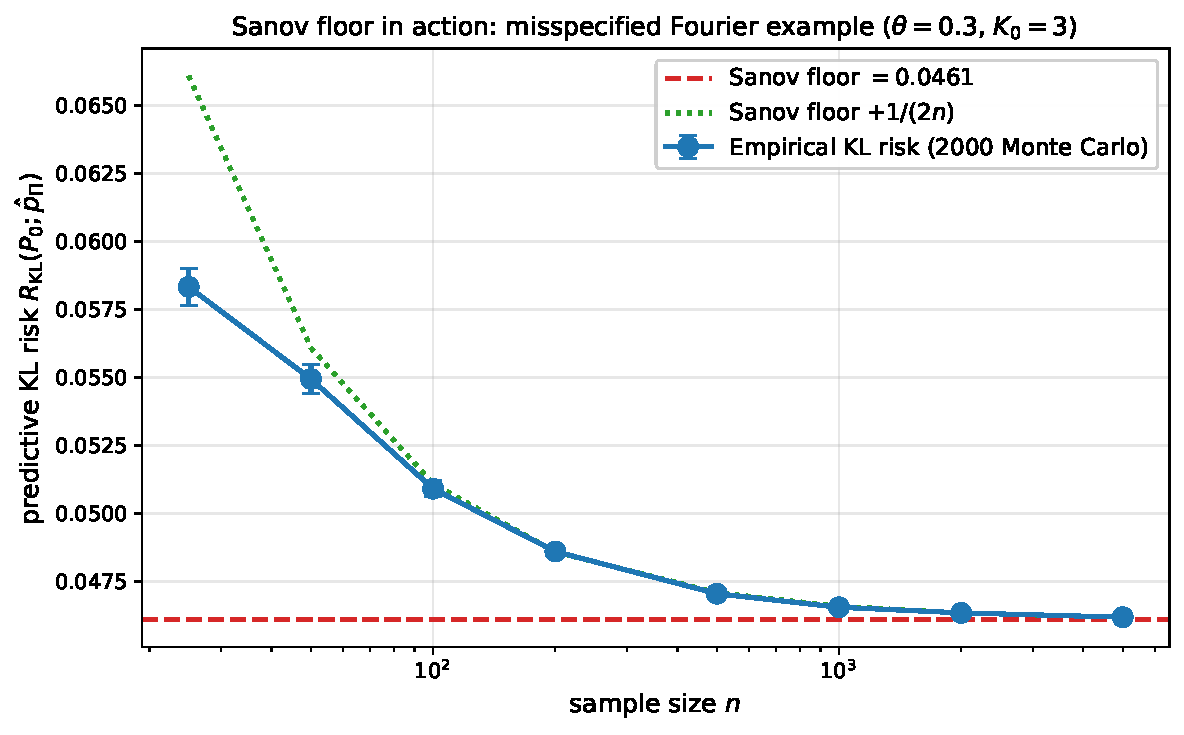
\includegraphics[width=0.72\textwidth]{sanov_floor}
\caption{Empirical predictive Bayes risk converges to the theoretical Sanov floor $\KL(P_0\|\Pi^*P_0) \approx 0.04608$ at rate $1/(2n)$. The Sanov floor is the structural irreducible risk imposed by the prior's inability to represent the true frequency mode of $p_0$.}
\label{np:fig:sanov-floor}
\end{figure}

\subsubsection{A second example: Bernoulli with calibration prior}\label{np:sec:bernoulli-ex}

To show that the framework is not specific to Gaussian / cosine geometry, we work out a Bernoulli example with a calibration prior.

\paragraph{Setup.} Take $\X = \{0, 1\}$ with counting measure. The true distribution is $\mathrm{Ber}(p_0)$ for some unknown $p_0 \in (0, 1)$. The prior places a Beta$(\alpha, \beta)$ on the success probability, but \emph{truncated} to a known calibration window $[q_-, q_+] \subset (0, 1)$ that may or may not contain $p_0$. The prior is misspecified when $p_0 \notin [q_-, q_+]$.

\paragraph{Reverse I-projection.} Since $\supp(\Pi) = [q_-, q_+]$, the reverse I-projection of $\mathrm{Ber}(p_0)$ onto this support minimizes
\[
\KL\bigl(\mathrm{Ber}(p_0)\,\big\|\,\mathrm{Ber}(q)\bigr) \;=\; p_0\log\frac{p_0}{q} + (1-p_0)\log\frac{1-p_0}{1-q},
\]
a strictly convex function of $q \in (0, 1)$ with unconstrained minimum at $q = p_0$. Constrained to $[q_-, q_+]$,
\begin{equation}\label{np:eq:bern-iproj}
q^* \;:=\; \Pi^*\bigl(\mathrm{Ber}(p_0)\bigr) \;=\;
\begin{cases}
q_- & \text{if } p_0 < q_-,\\
p_0 & \text{if } p_0 \in [q_-, q_+],\\
q_+ & \text{if } p_0 > q_+.
\end{cases}
\end{equation}

\paragraph{Sanov rate.} For $p_0 \notin [q_-, q_+]$,
\begin{equation}\label{np:eq:bern-sanov}
\KL(P_0\|\Pi^*P_0) \;=\; p_0\log\frac{p_0}{q^*} + (1-p_0)\log\frac{1-p_0}{1-q^*}.
\end{equation}
Local expansion near the boundary: for $p_0 = q_- - \eps$ with $\eps$ small,
\[
\KL\bigl(\mathrm{Ber}(p_0)\,\big\|\,\mathrm{Ber}(q_-)\bigr) \;=\; \frac{\eps^2}{2\,q_-(1-q_-)} + O(\eps^3),
\]
the standard Fisher quadratic for Bernoulli with curvature $1/(q_-(1-q_-))$.

\paragraph{Contraction rate.} The truncated Beta posterior on $[q_-, q_+]$ contracts to $q^*$. In the misspecified case $p_0 < q_-$, the log-likelihood has slope of order $n$ at the boundary $q_-$, so the posterior of $q - q_-$ is approximately exponential with rate $\lambda_n = n(q_- - p_0)/\{q_-(1-q_-)\}$ and concentrates at $q_-$ at rate $O_{\PP}(1/n)$; the Kleijn--van der Vaart theorem, which needs an interior pseudo-true parameter, does not apply. The posterior mean $\bar q_n$ satisfies $\E(\bar q_n - q_-) = \lambda_n^{-1}(1+o(1))$, and the predictive KL satisfies
\[
J_n(\Pi, \mathrm{Ber}(p_0)) \;=\; \frac{q_-(1-q_-)}{2\,(q_- - p_0)^2\,n^2}\,(1+o(1)),
\]
of order $n^{-2}$ rather than $n^{-1}$. In the well-specified case $p_0 \in (q_-, q_+)$, standard Bernstein--von Mises gives $J_n = 1/(2n) + o(1/n)$.

\paragraph{Combined risk.} For $p_0 \notin [q_-, q_+]$ the cross term is not $o(1/n)$: for $q \in [q_-, q_+]$, $\KL(\mathrm{Ber}(p_0)\|\mathrm{Ber}(q)) - \KL(\mathrm{Ber}(p_0)\|\mathrm{Ber}(q^*)) - \KL(\mathrm{Ber}(q^*)\|\mathrm{Ber}(q)) = (q^* - p_0)\{\mathrm{logit}\,q - \mathrm{logit}\,q^*\}$, which is first order in $q - q^*$. With the posterior mean at distance $q^*(1-q^*)/(n|q^* - p_0|)\,(1+o(1))$ from $q^*$ on average, this gives $r_n = n^{-1}(1+o(1))$, and the master decomposition reads
\[
R_{\KL}(P_0;\hat p_\Pi) \;=\; \underbrace{p_0\log\tfrac{p_0}{q^*} + (1-p_0)\log\tfrac{1-p_0}{1-q^*}}_{\text{Sanov floor}} \;+\; \underbrace{O(n^{-2})}_{\text{contraction}} \;+\; \underbrace{\frac{1}{n}\,(1+o(1))}_{\text{cross term}}.
\]
The Bernoulli example showcases the same dichotomy as the Fourier example, with boundary-projected $q^*$ playing the role of $\mathrm{Unif}$ and the Fisher curvature $1/\{q^*(1-q^*)\}$ replacing the cosine-family curvature $1$.

\subsubsection{Interpretation}\label{np:sec:ex-summary}

The Fourier and Bernoulli examples illustrate four structural features of the general decomposition of Theorem~\ref{np:thm:abc-csiszar}; the misspecified Bernoulli case departs from the Fourier pattern in the second and third:

\begin{enumerate}\setlength\itemsep{1pt}
\item \emph{Population-level Sanov floor:} a non-vanishing $\KL(P_0\|\Pi^*P_0)$ that depends only on $P_0$ and the prior support, not on $n$.
\item \emph{Parametric contraction:} a $J_n = c/n + o(1/n)$ term when the parameter of $\Pi^*P_0$ is interior to the prior support, where $c$ is half the Fisher information at $\Pi^*P_0$ times the limiting variance of $\sqrt n$ times the posterior mean ($c=1/2$ in the Fourier example and when well specified). At a boundary I-projection (misspecified Bernoulli) the posterior contracts at rate $1/n$ and $J_n$ is of order $n^{-2}$.
\item \emph{Cross term:} a residual $r_n = o(1/n)$ in the Fourier example, thanks to the Csisz\'ar Pythagorean equality \eqref{np:eq:ex-pythagorean}; at the boundary I-projection \eqref{np:eq:bern-iproj} of the misspecified Bernoulli example the cross term is first order in $\bar q_n - q^*$ and carries the leading excess, $r_n = n^{-1}(1+o(1))$.
\item \emph{Diagnostic match:} $n \cdot \text{residual}$ tends to an explicit constant, $1/2$ for the Fourier example and $1$ for the misspecified Bernoulli example; in the Fourier Monte Carlo it stays within $0.04$ of $1/2$ for $n \ge 100$.
\end{enumerate}

\subsection{Implementation}\label{np:sec:implementation}

The decomposition of Theorem~\ref{np:thm:abc-csiszar} produces a three-step diagnostic that any practitioner can apply to a Bayesian nonparametric prediction problem.

\subsubsection{Three-step diagnostic}\label{np:sec:impl-diagnostic}

\begin{enumerate}
\item \emph{Diagnose misspecification.} Compute or estimate the Sanov rate $\KL(P_0\|\Pi^*P_0)$ via the reverse I-projection of Examples~\ref{np:ex:dp-iproj}--\ref{np:ex:lgp-iproj}. For priors whose Kullback--Leibler support contains $P_0$ (a Dirichlet process mixture whose bandwidth prior charges every neighborhood of $0$, the canonical P\'olya tree) the Sanov rate vanishes under Assumption~\ref{np:ass:density}, and the predictive risk decays. For restricted-support priors (logistic-GP with finite RKHS, finite-parameter mixture priors, parametric exponential families) the Sanov rate is generically positive, and the predictive risk has an irreducible floor.

\item \emph{Compute the contraction rate.} The Hellinger contraction rate $\eps_n$ is available from the rate-of-contraction literature (Ghosal, Ghosh and van der Vaart, 2000; van der Vaart and van Zanten, 2008; van der Vaart and van Zanten, 2009; Castillo, 2017). The corresponding KL contraction rate is $O(\eps_n^2)$ (Theorem~\ref{np:thm:master}); Table~\ref{np:tab:kappas} gives the polylog factors of the bounds for the three priors of Section~\ref{np:sec:apps}. The Wong--Shen (1995) condition (Assumption~\ref{np:ass:wongshen}) is the bridge between Hellinger and KL contraction; it holds for every prior once restricted to densities with $\pi^* \le M_{\rm WS}\,p$, and the remaining densities enter through the tail condition of Theorem~\ref{np:thm:master}.

\item \emph{Combine.} The predictive risk is dominated by the Sanov term in the misspecified regime and the contraction term in the well-specified regime; the cross term is asymptotically negligible (Theorem~\ref{np:thm:abc-csiszar}). For the KS-truncated predictive density of Section~\ref{np:sec:ks-truncation}, Conjecture~\ref{np:conj:ks-mdp} puts the truncation level at the KS distance $\Delta_n$ between $P_0$ and $\Pi^*P_0$, which is $\sqrt{2\log n}$ at the detection boundary.
\end{enumerate}

The diagnostic admits a frequentist interpretation: the Sanov rate at Step 1 equals the mean per observation of the log-likelihood-ratio statistic for testing $P = \Pi^*P_0$ against $P = P_0$. When this Sanov rate is computed from data via a plug-in estimator $\widehat{\KL}(P_0\|\Pi^*P_0)$, a value comparable to or smaller than $\eps_n^2$ indicates approximate well-specification; a value substantially larger than $\eps_n^2$ indicates misspecification with a non-trivial Sanov floor.

\subsubsection{Implementation notes per prior}\label{np:sec:impl-priors}

\paragraph{Dirichlet-process mixture of Gaussians.} The DPM-of-Gaussians predictive is computed by MCMC over both the latent partition structure (using the Chinese restaurant\index{Chinese restaurant process} process (Blackwell and MacQueen, 1973)) and the bandwidth hyperparameter $h$. The bandwidth selection can be integrated out via the marginal likelihood, with the data-adaptive bandwidth $\hat h_n$ standing in for the optimum $h_n^* = n^{-1/(2\beta+1)}$; Theorem~\ref{np:thm:dp} assumes that $\hat h_n$ stays within constant factors of $h_n^*$. Standard software (the \texttt{DPpackage} R library, or the \texttt{numpyro} DP modules in Python) handles this efficiently for $n$ up to several thousand; for larger $n$, slice-sampling (Walker, 2007) or variational-inference approximations are practical.

\paragraph{Canonical P\'olya tree.} The P\'olya tree predictive admits a closed form at each truncation level $L$: at depth $L$, the predictive density on cell $B_\eps$ at the finest level is $(\beta_\eps + n_\eps)/(2\beta_\eps + n_{\rm parent})$ times the conditional probability along the path. The truncation level $L_n^*$ can be selected by maximizing the marginal likelihood across $L \in \{1,\dots,\log_2 n\}$, a grid of $b_n = \log_2 n$ levels, on which the heuristic of Remark~\ref{np:rem:adaptive} puts the price of adaptation at a power of $\log b_n \asymp \log\log n$, within the $\log n$ factor of Theorem~\ref{np:thm:pt}. Lavine's (1992) original recommendation $\beta_\eps = c\,|\eps|^2$ is what makes the P\'olya tree absolutely continuous with bounded density, a crucial feature for our Assumption~\ref{np:ass:density}.

\paragraph{Logistic-Gaussian process.} The LGP predictive is non-conjugate and requires MCMC for exact inference; standard NUTS (Hoffman and Gelman, 2014) or variational inference\index{variational inference} (Titsias and L\'azaro-Gredilla, 2014) suffice. The length-scale hyperparameter $A$ is sampled from its conditional posterior (typically log-normal), with the resulting marginal predictive density obtained by Monte Carlo averaging. For our Monte Carlo experiments (Section~\ref{np:sec:gp-mc}), we used a penalized-MLE approximation in a cosine basis with Sobolev-2 penalty (Mat\'ern-$3/2$ kernel spectral decay), which produced empirical slopes within $0.001$ of the theoretical prediction.

\paragraph{KS-truncated predictive density.} The KS-truncation \eqref{np:eq:ks-trunc} is computationally trivial once $F_n$ has been evaluated on a grid: clip the empirical-process residual $F_n(x) - F_\Pi^*(x)$ at $\pm a/\sqrt{n}$, with $a$ set as in Conjecture~\ref{np:conj:ks-mdp}. The resulting CDF is differentiated and kernel-smoothed (bandwidth $h_n \to 0$) to obtain a smooth predictive density. For $n = 1{,}000$, this computation takes milliseconds in standard Python (\texttt{numpy}, \texttt{scipy.stats}).

\paragraph{Reproducibility.} Python scripts reproducing all Monte Carlo experiments of this section, including Figures~\ref{np:fig:ks-mdp}, \ref{np:fig:dpm-rate}, \ref{np:fig:pt-rate}, \ref{np:fig:lgp-rate}, \ref{np:fig:combined-priors}, \ref{np:fig:iproj-geom}, and~\ref{np:fig:sanov-floor}, and Table~\ref{np:tab:mc}, and the testing experiment of Section~\ref{np:sec:rs-mc} (its table and Figure~\ref{np:fig:rs-bayes}), are available in the book's accompanying code repository. The scripts require only \texttt{numpy}, \texttt{scipy}, and \texttt{matplotlib} (Python 3.10+), and run in a few minutes per figure on a standard laptop. No specialized Bayesian-nonparametric library is required: the experiments use direct numerical integration of the posterior or oracle-bandwidth grid search rather than MCMC, allowing the reader to verify the predictive risk decompositions directly from the empirical CDF and the reverse I-projection.

\subsection{Discussion}\label{np:sec:disc}

This discussion gathers the threads of the section and places them in the wider program. We recap the moderate-deviation reading and the empirical distribution function as the nonparametric Bayes solution, note the link to the Polson--Zantedeschi work, and then turn to what is new and the open problems that remain.

\paragraph{The moderate-deviation program.}

The present section completes the nonparametric branch of a four-paper program:

\begin{center}
\renewcommand{\arraystretch}{1.15}
\begin{tabular}{@{}lll@{}}
\toprule
\textbf{Loss / setting} & \textbf{Reference} & \textbf{Adaptive penalty} \\
\midrule
$0/1$ (testing) & arXiv:2602.11132 & $\sqrt{\log n}$ \\
$L^2$ (sparse estimation) & arXiv:2604.01266 & $\log(d_n/s_n)$ \\
$\KL$ (sparse prediction) & arXiv:2604.01266 & $\log(d_n/s_n)$ \\
$\KL$ (nonparametric prediction) & this section & $(\log n)^{\kappa(\Pi)}$ \\
GOF testing & arXiv:2602.15297 & $\sqrt{2\log n}$ \\
KS-truncated prediction & this section, Sec.~\ref{np:sec:ks} & $\sqrt{2\log n}$ (conjectured) \\
\bottomrule
\end{tabular}
\end{center}

In the testing and sparse rows the adaptive penalty arises from balancing the cost of an unknown structural parameter against the contraction rate at the moderate-deviation scale. The KS row holds at the detection boundary $\Delta_n = \sqrt{2\log n}$ (Conjecture~\ref{np:conj:ks-mdp}), and in the nonparametric row $(\log n)^{\kappa(\Pi)}$ is the allowance of Theorems~\ref{np:thm:dp}--\ref{np:thm:gp}, of which the balancing heuristic of Remark~\ref{np:rem:adaptive} accounts for a power of $\log\log n$. The unification is structural: a single Rubin--Sethuraman risk-balancing argument, applied to the appropriate test statistic at the right moderate-deviation scale, produces all the polylogarithmic factors seen in the literature on Bayesian sparse regression, parametric testing, and goodness-of-fit testing.

\paragraph{The empirical CDF as the nonparametric Bayes score function.}

The KS-truncated predictive density of Section~\ref{np:sec:ks-truncation} crystallizes a structural analogy between parametric and nonparametric Bayesian prediction that deserves emphasis. In the parametric horseshoe paper (Polson, Sokolov and Zantedeschi, 2026c, arXiv:2604.01266), the marginal-likelihood score $\nabla\log m_n(X^{(n)})$ is the natural data-summary statistic on which Bayes-optimal sparse calibration operates, with the calibration scale set at the moderate-deviation envelope $\sqrt{2\log p}$ (where $p$ is the model dimension). In our nonparametric setting, with $P_0$ at the detection boundary $\Delta_n = \sqrt{2\log n}$ from $\Pi^*P_0$, the empirical CDF $F_n(x)$ plays the analogous role: it is the natural data-summary on which Bayes-optimal nonparametric calibration operates, with the calibration scale set at the same moderate-deviation envelope $\sqrt{2\log n}$. The analogy is precise: in both settings, the relevant moderate-deviation tail is Gaussian (with bridge-scale variance for $F_n$, and Fisher-information-scale variance for $\nabla\log m_n$); in both settings, the Rubin--Sethuraman risk balance produces the canonical $\sqrt{2\log\cdot}$ threshold; and in both settings, the empirical-process / score-function statistic is a sufficient summary of the data for Bayes-optimal prediction.

This analogy suggests a broader program: \emph{find the right data-summary statistic for the given Bayes risk, calibrate it at the moderate-deviation scale}. Examples include the K-S statistic for goodness-of-fit testing; the Cram\'er--von Mises statistic for an integrated alternative to KS (Anderson and Darling, 1952); the marginal-likelihood score for parametric sparse selection (Polson, Sokolov and Zantedeschi, 2026c, arXiv:2604.01266); the empirical CDF for nonparametric prediction (this section); and the empirical measure on partition cells for tree-structured priors (Castillo, 2017). In each case, the choice of summary statistic is dictated by the prior architecture (full-support Bayesian nonparametrics vs.\ parametric sparse priors), and the calibration scale is set by the corresponding moderate-deviation envelope.

\paragraph{Connection to the Polson--Zantedeschi program.}

The Sanov term of Theorem~\ref{np:thm:abc-csiszar} has a direct geometric interpretation via the three Polson--Zantedeschi papers (2025a, 2025b, 2026a), each of which addresses a different facet of the same I-projection / exchangeability / large-deviation triple.

\emph{De Finetti + Sanov = Bayes (Polson and Zantedeschi, 2025a).} The tilted de Finetti theorem of Polson and Zantedeschi (2025a) states that conditioning an exchangeable sequence on empirical-moment constraints produces an I-projection of the de Finetti baseline as the predictive limit. The mechanism is large-deviation typicality: under empirical-moment conditioning, typical sequences concentrate exponentially fast on the I-projected baseline, and the predictive law for any fixed block converges to the I-projection. That I-projection minimizes over the first argument of the divergence and our $\Pi^*P_0$ over the second, so the two agree in the dual case of Section~\ref{np:sec:sanov}, a moment constraint paired with the exponential family it generates; in general $\Pi^*P_0$ is the predictive limit of the prior $\Pi$ when the data-generating measure is $P_0$ because the posterior concentrates near it (Kleijn and van der Vaart, 2006). In the dual case, the misspecified case of our Theorem~\ref{np:thm:abc-csiszar} (Sanov floor $\KL(P_0\|\Pi^*P_0) > 0$) is a truth $P_0$ outside the exponential family, for which the exponentially tilted predictive law matches the moments of $P_0$ but differs from $P_0$.

\emph{Bayesian prediction under moment conditioning (Polson and Zantedeschi, 2025b).} For a fixed baseline on a finite partition, the Gaussian localization of Polson and Zantedeschi (2025b) sharpens the tilted de Finetti theorem with explicit curvature-controlled rates. The information-geometric Hessian $H^*$ of the KL functional restricted to the constraint manifold controls the rate at which the conditioned empirical type concentrates on the I-projection, with smallest eigenvalue of $H^*$ governing that concentration at finite $n$. This localization is not a local asymptotic normality expansion, and parameter contraction there is governed by the parameter information $\Info_{\theta,r}$ of~\eqref{eq:param-info}, not by $H^*$. Our Wong--Shen Assumption~\ref{np:ass:wongshen} is only analogous: the inequality $\KL(\pi^*\|p) \le C_{\rm WS}\,\dH(P,\Pi^*P_0)^2$ is the population-level statement that the KL functional has bounded curvature in a Hellinger neighborhood of $\pi^*$, but $C_{\rm WS}$ is not determined by $H^*$. The Polson--Zantedeschi local quadratic expansion (2025b) therefore motivates, but does not enter, the bound on our contraction term $J_n$.

\emph{Martingale posterior predictive coherence (Polson and Zantedeschi, 2026a).} The Hausdorff moment hierarchy of Polson and Zantedeschi (2026a) extends single-step prediction to the multi-step setting, exploiting Bernstein's expansion of CDFs in Hausdorff moments. The single-step machinery developed here is the first step of that hierarchy. Multi-step predictive risk under the present framework involves coupling structure across prediction horizons that is qualitatively different from single-step risk: the predictive law of the next $m$ observations given data through time $n$ is the $m$-fold product of the latent law, weighted by the posterior on that law. The Polson--Zantedeschi Hausdorff machinery (2026a) provides the natural framework for analyzing multi-step risk, and we conjecture that an analogous Aitchison--Barron--Clarke decomposition holds at each step of the hierarchy. For the joint law of the next $m$ observations the chain rule already gives one: its KL risk is the sum of the single-step risks at sample sizes $n,\dots,n+m-1$, so the Sanov floor is $m\,\KL(P_0\|\Pi^*P_0)$ and the contraction term is $\sum_{j<m}J_{n+j}(\Pi,P_0)$; for a single observation at lag $m$, exchangeability makes the predictive law the single-step one, so neither term depends on $m$.

The three Polson--Zantedeschi papers together identify the predictive \emph{limit} of nonparametric Bayes under exchangeability and moment conditioning; the present section identifies the \emph{rate} at which the risk approaches that limit. The unification of these perspectives places the moderate-deviation Bayes-risk program within the broader framework of de Finetti's theorem, Sanov's theorem, and the Csisz\'ar I-projection geometry, providing a coherent foundation for Bayesian prediction under both well- and misspecified models.

\paragraph{Provenance and new contributions.}

\emph{Inputs (classical).} The chain rule \eqref{np:eq:abc-chain} is Aitchison (1975); the reverse I-projection pivot is implicit in Clarke--Barron (1990). The rates used in the proofs of Theorems~\ref{np:thm:pt} and~\ref{np:thm:gp} are from Castillo (2017) and van der Vaart and van Zanten (2008, 2009), the latter for the squared exponential kernel; Theorem~\ref{np:thm:dp} assumes its bandwidth step. The Csisz\'ar Pythagorean equality of Remark~\ref{np:rem:csiszar} is Csisz\'ar (1975). The Carota--Parmigiani Bayes-factor analysis is Carota and Parmigiani (1996) and Carota, Parmigiani, and Polson (1996).

\emph{Inputs (companion).} The conditional Sanov theorem (Theorem~\ref{np:thm:tilted}) is Polson and Zantedeschi (2025a); the Kolmogorov--Smirnov calibration of Theorem~\ref{np:thm:rs} follows the goodness-of-fit testing paper of Polson, Sokolov and Zantedeschi (2026b, arXiv:2602.15297), and Datta, Polson, Sokolov, and Zantedeschi (2026) calibrate parametric tests on the same scale. The reduced Hessian $H^*$ contrasted above with Assumption~\ref{np:ass:wongshen} is Polson and Zantedeschi (2025b).

\emph{New contributions.} (i) The decomposition of Theorem~\ref{np:thm:abc-csiszar} with the explicit Cauchy--Schwarz cross-term bound \eqref{np:eq:cross} and the asymptotic dichotomy. (ii) The Fubini factorization \eqref{np:eq:fubini-risk} of nonparametric predictive Bayes risk via the empirical CDF, with the structural correspondence to the Carota--Parmigiani Bayes-factor analysis (Section~\ref{np:sec:cp}). (iii) The KS-truncated predictive density of Definition~\ref{np:def:ks-pred} and Conjecture~\ref{np:conj:ks-mdp} on its Bayes-risk-optimal moderate-deviation truncation level, supported by Monte Carlo (Figure~\ref{np:fig:ks-mdp}). (iv) The empirical-CDF / score-function unification statement (above). (v) The misspecified Fourier worked example of Section~\ref{np:sec:miss-example} with closed-form Sanov rate \eqref{np:eq:ex-sanov}, exhibiting the floor numerically to four decimal places (Figure~\ref{np:fig:sanov-floor}). (vi) Monte Carlo illustrations of Theorems~\ref{np:thm:dp}--\ref{np:thm:gp} for all three standard priors (Figures~\ref{np:fig:dpm-rate}--\ref{np:fig:combined-priors}). (vii) The unified placement of the four-paper moderate-deviation Bayes-risk program within the Polson--Zantedeschi tilted de Finetti / I-projection geometric framework.

\paragraph{Open problems.}

\begin{itemize}
\item \emph{Rigorous proof of Conjecture~\ref{np:conj:ks-mdp}.} A KMT-type strong-approximation argument together with explicit Kolmogorov-tail constants for the empirical process $F_n - F_\Pi^*$ would convert Conjecture~\ref{np:conj:ks-mdp} into a theorem. The Monte Carlo of Section~\ref{np:sec:ks-mc} does not settle it (its minimizer stays within $11\%$ of $\Delta_n$ for $n \ge 500$, at six sample sizes with $15$ replications each), and the precise calibration of the bias-variance trade-off under both well- and misspecified regimes remains open. We expect that the appropriate proof will use Talagrand's concentration inequality (Talagrand, 1995) for the empirical process to obtain uniform-in-$a$ tail bounds, combined with a Lindeberg-replacement argument to handle the KL non-linearity.

\item \emph{Sharp constants in Theorems~\ref{np:thm:dp}--\ref{np:thm:gp}.} The contraction rates of Theorems~\ref{np:thm:dp}--\ref{np:thm:gp} are determined only up to multiplicative constants. A Clarke--Barron-style second-order expansion of $J_n$ for each of the three example priors would identify the leading constants in terms of the prior density at the reverse I-projection $\Pi^*P_0$, by analogy with the parametric $-\log\pi(P_0)$ term in Clarke and Barron (1990). The Polson--Zantedeschi local quadratic expansion of the KL functional (2025b) provides the natural starting point.

\item \emph{Multi-step prediction.} The Polson--Zantedeschi Hausdorff moment hierarchy (2026a) suggests a direct extension to multi-step predictive risk. The cross-step coupling structure is qualitatively different from the single-step case treated here, and we conjecture that a hierarchy of Aitchison--Barron--Clarke decompositions holds at each step. For the joint law of the next $m$ observations the chain rule gives the decomposition directly, with floor $m\,\KL(P_0\|\Pi^*P_0)$; which multi-step risk the hierarchy should control, and its decomposition, are open.

\item \emph{Non-Csisz\'ar geometries.} For Amari $\alpha$-divergence predictive risks (Komaki, 2001), the I-projection takes place in $\alpha$-geometry rather than Csisz\'ar I-geometry, and the analogous decomposition is open. The $\alpha = 1$ case corresponds to KL ($I$-divergence in Csisz\'ar's notation), and the $\alpha = -1$ case to reverse KL. For Bregman-divergence losses more general than KL, a similar decomposition should hold with the corresponding $\alpha$-projection replacing $\Pi^*P_0$, but the analogue of the Cauchy--Schwarz cross-term bound \eqref{np:eq:cross} requires the relevant generalization of Csisz\'ar's inequality.

\item \emph{Dependent observations.} Theorem~\ref{np:thm:rs} uses i.i.d.\ observations through the Kolmogorov tail bound for the empirical process. Extension to weakly dependent processes (mixing, Markov, stationary sequences) requires the Berkes--Philipp (1979) or Bradley (1983) strong-approximation embeddings, which give Brownian-bridge couplings under mixing conditions. Whether the Polson--Zantedeschi Gaussian localization (2025b) also extends to dependent observations under appropriate mixing assumptions is open, since it is proved for independent baseline draws; an extension would suggest that the entire framework of this section has a dependent-data analogue, with the moderate-deviation scale modified by the long-run variance of the relevant statistic.

\item \emph{Beyond bounded densities.} Assumption~\ref{np:ass:density} requires the data-generating density to be bounded above and below. For unbounded densities (e.g., heavy-tailed distributions or densities supported on unbounded domains), the Csisz\'ar $\chi^2$/KL inequality fails and the cross-term bound \eqref{np:eq:cross} must be replaced by a more refined argument. The extension is open and would require careful empirical-process analysis on unbounded domains.

\item \emph{Bernstein--von Mises in the predictive setting.} The Kleijn--van der Vaart misspecified Bernstein--von Mises theorem (2012) gives a Gaussian limit for the posterior distribution under misspecification, with variance $H^{-1}$ while its center has the sandwich sampling variance $H^{-1}KH^{-1}$. The implications for the cross term $r_n$ in Theorem~\ref{np:thm:abc-csiszar} (specifically, the higher-order behavior beyond the Cauchy--Schwarz bound) remain to be worked out. The worked example of Section~\ref{np:sec:miss-example} suggests $r_n = o(1/n)$ in this regime, but a general statement is open.
\end{itemize}




\subsection*{Worked example: the Dirichlet-process predictive}
This example shows how a nonparametric prior learns any distribution while still behaving like a prior at small sample sizes.

For the Dirichlet-process predictive with base $G_0$ and concentration $\alpha$, the predictive distribution after $n$ observations is $\frac{\alpha}{\alpha+n}G_0+\frac{n}{\alpha+n}\Phat_n$, a convex blend of prior and empirical. As $n\to\infty$ the empirical dominates at rate $\alpha/n$, so the nonparametric predictive is consistent for any true $P$ with no parametric assumption, and $\alpha$ is the effective prior sample size.

Read as a predictive, the formula is a running average that starts at the prior guess $G_0$ and is pulled toward the data at rate $n/(\alpha+n)$; the concentration $\alpha$ is literally the number of prior pseudo-observations, so a small $\alpha$ forgets the prior quickly and a large one holds onto it. Because the empirical part imposes no functional form, consistency follows for any true $P$.

\paragraph{Summary.}
The predictive Bayes risk of a nonparametric prior splits into a Sanov floor $\KL(P_0\|\Pi^*P_0)$ (the divergence from the truth to its reverse I-projection on the prior support), a contraction term $J_n$, and a cross term at most $C(\sqrt{\KL(P_0\|\Pi^*P_0)\,J_n}+J_n)$ (Theorem~\ref{np:thm:abc-csiszar}). The floor vanishes when $P_0$ lies in the Kullback--Leibler support of the prior, as for the Dirichlet-process mixture with a bandwidth prior that charges every neighborhood of $0$ and for the canonical P\'olya tree; in the Fourier example it is positive, has a closed form, and is approached at the rate $1/(2n)$. For the Kolmogorov--Smirnov test the Rubin--Sethuraman balance puts the Bayes threshold at $\Delta_n/2$ in the interior regime and at $3\Delta_n/8$ at the canonical boundary (Theorem~\ref{np:thm:rs}), and Conjecture~\ref{np:conj:ks-mdp} puts the optimal truncation level of the KS-truncated predictive at the KS distance $\Delta_n$.

\subsection*{Problems}
\begin{enumerate}[leftmargin=2.2em,itemsep=2pt]
\item Write the predictive Bayes risk as a Fubini integral of the pointwise posterior risk and identify the minimizing rule.
\item Compute a Sanov floor for the risk in a simple closed-form example.
\item Show that the predictive is consistent under the true data-generating process without assuming a parametric model.
\item Compare the Dirichlet-process predictive of the worked example with the plug-in empirical distribution $\Phat_n$ on a finite alphabet of $k$ letters, each of positive probability under the truth and under $G_0$: show that the plug-in has infinite expected KL risk, while the risk of the predictive is $(k-1)/(2n)+o(1/n)$.
\item Discuss how exchangeability licenses the empirical-process construction.
\end{enumerate}

\src{Nonparametric Predictive Bayes Risk (Polson and Zantedeschi, 2026i, JASA submission); De Finetti + Sanov = Bayes (2509.13283); Bayes Risk for Goodness of Fit Tests (2602.15297); Bayesian Prediction under Moment Conditioning (2510.20742).}

%====================================================================================================
%====================================================================================================

\shorthead{Minimum Description Length and Coding}
\section{Minimum Description Length and the Coding View of Bayes}\label{ch:mdl}

\noindent\textbf{Thesis.} The best model of the data is the shortest program that
generates it, and under the Kraft inequality that principle is Bayesian inference
under a coding prior: every probability distribution is a code and every code a
distribution, so minimizing description length is maximizing evidence. This
section is the information-theoretic completion of the evidence theory of Sections~\ref{ch:evalues}, \ref{ch:deviations}, and~\ref{ch:evmdp} (evidence, testing, and deviation rates). Rissanen's minimum description length\index{minimum description length}, Wallace's minimum
message length, MacKay's Bayesian evidence with its Occam factor, Barndorff-Nielsen's
$p^\ast$ modified profile likelihood, Drton's singular BIC, and the horseshoe
compression bound of Theorem~\ref{hs:thm:super} are one construction read at different resolutions. The
log-marginal-likelihood is a codelength; the Occam factor is the parametric
volume the code must pay for; the real log-canonical threshold is what that volume
becomes when the Fisher information degenerates; and the horseshoe is the code that
charges almost nothing for a sparse signal. Model selection by evidence differs from
cross-validation in that it pays the code once: the negative log evidence is one codelength, the sum over observations of the log loss of each observation given those before it.

% ══════════════════════════════════════════════════════════════════════════════

The best model of data is the shortest program that generates it. This single
principle, variously attributed to Occam, Leibniz, Kolmogorov, and
Solomonoff, underlies a remarkable convergence of ideas across information
theory, Bayesian statistics, computational learning theory, and algebraic
geometry.

Minimum Description Length (MDL), developed by Rissanen (1978) as a
computable statistical criterion, is the direct operationalization of
Kolmogorov complexity (Kolmogorov, 1965; Chaitin, 1966, 1969) for model selection.
Minimum Message Length (MML), developed independently by Wallace and Boulton (1968)
and refined by Wallace and Freeman (1987), provides the Bayesian counterpart.
MacKay (1992); MacKay (2003) developed the Bayesian evidence framework,
arguing that the marginal likelihood, the ``evidence'' for a model, is
preferable to cross-validation as a model selection device,
automatically implementing Occam's razor through what he called the Occam
factor.

This section traces connections among six major threads: (1)~algorithmic
information theory (Kolmogorov, 1965; Chaitin, 1969; Solomonoff, 1964; Li and Vit\'anyi, 2008);
(2)~statistical MDL/MML (Rissanen, 1978; Rissanen, 1987; Wallace and Freeman, 1987);
(3)~Bayesian evidence and cross-validation (MacKay, 1992; MacKay, 2003);
(4)~higher-order likelihood (Barndorff-Nielsen, 1983; Barndorff-Nielsen, 1986);
(5)~sparse Bayesian inference (Carvalho, Polson and Scott, 2010; Polson and Scott, 2010); and
(6)~algebraic model selection (Drton and Plummer, 2017; Watanabe, 2009).

Throughout, the Kraft inequality serves as the foundational bridge: every
probability distribution defines a code, and every code defines a probability
distribution. Model selection by code-length minimization is Bayesian
inference under a coding prior.

% ══════════════════════════════════════════════════════════════════════════════
\subsection{The Kraft Inequality: Probability as Code}
% ══════════════════════════════════════════════════════════════════════════════

For any uniquely decodable binary code with lengths $\ell_1, \ell_2, \ldots$,
the Kraft inequality states
\[
 \sum_{i} 2^{-\ell_i} \;\leq\; 1.
\]
Conversely, for any lengths satisfying this inequality a prefix-free code
exists achieving those lengths. This creates a canonical correspondence: every
probability distribution $p(x)$ defines a code with lengths
$\ell(x) = \lceil -\log_2 p(x) \rceil$, and every prefix-free code defines a
distribution $p(x) = 2^{-\ell(x)}$ (up to normalization). Shannon entropy
$H(X) = \E[-\log p(X)]$, divided by $\log 2$, is the expected code length in bits under the optimal code, to within one bit,
establishing that information and probability are two descriptions of the same
mathematical object.

Model selection by minimizing description length is equivalent to maximizing
the probability assigned by a prior over models and data. Bayesian inference
and coding are two faces of a single coin, a fact that underpins every
criterion discussed in this section.

% ══════════════════════════════════════════════════════════════════════════════
\subsection{Kolmogorov Complexity}
% ══════════════════════════════════════════════════════════════════════════════

The \emph{Kolmogorov complexity} $K(x)$ of a binary string $x$ is the length
of the shortest program $p$ on a universal Turing machine $U$ such that
$U(p) = x$:
\[
 K(x) \;=\; \min\bigl\{\,\ell(p) : U(p) = x\,\bigr\}.
\]
The \emph{Invariance Theorem} guarantees that $K_U(x)$ and $K_{U'}(x)$ differ
by at most a constant for any two universal machines $U, U'$, making $K$
machine-independent up to an additive constant. Chaitin connected $K$ to
randomness: a string is \emph{algorithmically random} if $K(x)\approx|x|$,
i.e., incompressible.

Solomonoff's \emph{universal prior}
$m(x) = \sum_{p:\,U(p)=x} 2^{-\ell(p)}$, for a prefix-free machine $U$ and with $K$ the prefix complexity, satisfies
$-\log_2 m(x) = K(x)+O(1)$, making Bayesian inference under $m$ identical to
Kolmogorov-complexity-based model selection. This universal prior dominates
all computable priors on strings. For prediction one uses its continuous counterpart, the monotone semimeasure $\mathbf M(x)$, the probability that a universal monotone machine fed random bits prints an output beginning with $x$; $\mathbf M$ dominates every computable measure $\mu$ on sequences and provides optimal sequential prediction: the
expected cumulative squared prediction error under $\mathbf M$ exceeds that of the best
computable predictor, the source $\mu$ itself, by at most $K(\mu)/2$, a finite bound independent of
sample size. $K(x)$ is upper semi-computable but not computable, placing the
ideal beyond any algorithmic reach.

The Lempel--Ziv algorithms (LZ77, LZ78, LZW) provide the computable bridge:
LZ compression achieves the entropy rate $H$ of any stationary ergodic source
without knowing the source distribution, and satisfies
$\ell_{\mathrm{LZ}}(x^n)/n \to H$ as $n\to\infty$. LZ is thus a computable
upper bound on $K(x)$ asymptotically tight to first order for typical outputs of the source (the gap is $o(1)$ per symbol), which is
why real compressors serve as practical proxies for Kolmogorov complexity in
the normalized compression distance (Section~\ref{sec:ncd}).

% ══════════════════════════════════════════════════════════════════════════════
\subsection{Rissanen's MDL: From Ideal to Computable}

Rissanen's minimum description length begins as an uncomputable ideal, the shortest program for the data, and is made operational by codes that approximate it. The two-part and normalized-maximum-likelihood codes below are the practical realizations, and both reproduce the same stochastic-complexity penalty.
% ══════════════════════════════════════════════════════════════════════════════

\subsubsection{Two-Part and Normalized-Maximum-Likelihood Codes}

Rissanen (1978) introduced MDL as a computable approximation to $K(x)$
for model selection. The two-part code version selects model $M$ minimizing
\[
 \MDL(M, x^n) \;=\; \ell(\htheta_M) \;+\; \ell(x^n \mid \htheta_M),
\]
where $\ell(\htheta_M)$ encodes the parameter estimate and
$\ell(x^n\mid\htheta_M) = -\log p(x^n\mid\htheta)$ is the Shannon code
length of data given the model. The penalty $(k/2)\log n$ for a $k$-parameter
model arises from encoding $\htheta$ to the precision that matters
($n^{-1/2}$) and independently recovers the BIC of Schwarz (1978).

Rissanen's mature formulation uses the \emph{Normalized Maximum Likelihood}
(NML) distribution:
\[
 p_{\mathrm{NML}}(x^n \mid M)
 \;=\;
 \frac{p(x^n \mid \htheta_{\mathrm{ML}}(x^n))}{\COMP(M)},
\]
where $\COMP(M) = \sum_{y^n} p(y^n \mid \htheta_{\mathrm{ML}}(y^n))$ is the
\emph{parametric complexity}. NML is optimal in the \emph{minimax regret}
sense: no code achieves smaller worst-case excess code length over all data
sequences of length $n$. The criterion $-\log p_{\mathrm{NML}}$ is MDL with
a game-theoretically grounded penalty.

Rissanen (1996) showed that, for a regular $k$-parameter model $M$ (a parameter set that is a compact subset of the interior of the full parameter space, a continuous and positive definite Fisher information $\Info(\theta)$ of one observation on it, and a maximum likelihood estimator that obeys a central limit theorem uniformly over it), the parametric complexity expands as
\[
 \log\COMP(M)
 \;=\;
 \frac{k}{2}\log\frac{n}{2\pi}
 \;+\;
 \log\int\sqrt{\det\Info(\theta)}\,d\theta
 \;+\; o(1).
\]
The leading term is the penalty $(k/2)\log n$ of the two part code, so both codes charge the same leading penalty and differ only in the constant. The integral is the volume of the model in the Fisher metric and the normalizer of the Jeffreys prior. For the Bernoulli model it equals $\int_0^1[\theta(1-\theta)]^{-1/2}d\theta=\pi$, and the expansion gives $\tfrac12\log n+\tfrac12\log(\pi/2)+o(1)$, the value that direct summation gives in the worked example at the end of this section, although $(0,1)$ is not compact.

% ══════════════════════════════════════════════════════════════════════════════
\subsection{MacKay's Bayesian Evidence and Cross-Validation}
\label{sec:mackay}

MacKay read model comparison as a three-level Bayesian hierarchy in which the evidence, not a held-out score, does the selecting. The subsections that follow lay out the three levels, isolate the Occam factor that penalizes complexity, and contrast evidence with cross-validation, automatic relevance determination, and the evidence lower bound.
% ══════════════════════════════════════════════════════════════════════════════

\subsubsection{Three Levels of Bayesian Inference}

MacKay (1992); MacKay (2003) articulated a hierarchical Bayesian framework
that situates model comparison within a three-level structure.

\textbf{Level~1, Parameter inference.}
Given model $M$ and data $D$, infer parameters $\theta$ via the posterior
$p(\theta\mid D,M)\propto p(D\mid\theta,M)\,p(\theta\mid M)$.

\textbf{Level~2, Hyperparameter optimization.}
Set hyperparameters by maximizing the evidence over a model family, yielding
automatic regularization.

\textbf{Level~3, Model comparison.}
Given data $D$, compare models via the \emph{evidence}
\[
 p(D\mid M) \;=\; \int p(D\mid\theta,M)\,p(\theta\mid M)\,d\theta,
\]
the marginal likelihood.

The evidence at Level~3 is the central quantity. Its ratio for two models is the
Bayes factor, whose logarithm is I.J.\ Good's weight of evidence (Good, 1950):
\[
 BF_{12} \;=\; \frac{p(D\mid M_1)}{p(D\mid M_2)}.
\]
The log Bayes factor is the difference in evidence (description length) between
two models, the MDL criterion difference.

\subsubsection{The Occam Factor}

The Laplace approximation\index{Laplace approximation} to the log evidence decomposes as
\[
 \log p(D\mid M)
 \;\approx\;
 \underbrace{\log p(D\mid\htheta,M)}_{\text{best-fit log-likelihood}}
 \;+\;
 \underbrace{\log \Omega_{\mathrm{Occam}}}_{\text{complexity penalty}},
\]
where the \emph{Occam factor} is
\[
 \Omega_{\mathrm{Occam}}
 \;=\;
 p(\htheta\mid M)\cdot(2\pi)^{k/2}\cdot|A|^{-1/2},
 \qquad
 A \;=\; -\frac{\partial^2\log p(D\mid\theta,M)}{\partial\theta\,\partial\theta^\top}
 \Bigg|_{\htheta}.
\]
The Occam factor $\Omega_{\mathrm{Occam}}$, at most $1$ once the data narrow the prior, equals the ratio of the
posterior volume to the prior volume in parameter space. A complex model
with diffuse prior $p(\theta\mid M)$ that achieves the same fit as a simpler
model incurs a larger Occam penalty, because it ``wasted'' prior probability
on parameter regions that did not explain the data. In regular models
$-\log\Omega_{\mathrm{Occam}}\approx(k/2)\log(n/2\pi)$ up to $O(1)$ terms, recovering the
BIC/MDL penalty from purely Bayesian principles.

The Occam factor has a precise information-geometric interpretation: it is the
ratio of the posterior ellipsoid volume to the prior volume, measured in units
of Fisher information. To leading order this is the Wallace--Freeman MML87 criterion
restated in geometric language.

\subsubsection{Evidence vs.\ Cross-Validation}

MacKay (1992) provided a systematic comparison of evidence-based model
selection against cross-validation (CV), arguing for the theoretical and
practical advantages of the former. The arguments are several and mutually
reinforcing, but they have limits: the negative log evidence is a cumulative predictive loss that scores each observation given only those before it, so its early terms rest on the prior and little data, and with a diffuse prior or a misspecified model the evidence can select a model that predicts worse than the one CV selects.

\begin{description}[leftmargin=0pt,itemsep=4pt]
\item[\normalfont\textbf{Computational efficiency.}]
 $K$-fold CV requires training the model $K$ separate times (typically
 $K=5$ or $10$), each on a data set of size $n(1-1/K)$. The evidence
 requires a single fit plus a one-time integration, analytic under the
 Laplace approximation. For models of moderate size this represents an order-of-magnitude
 computational saving; for large networks the log determinant of the $k\times k$
 Hessian $A$, which costs $O(k^3)$, is the bottleneck.

\item[\normalfont\textbf{Statistical efficiency.}]
 Leave-one-out CV trains on $n-1$ data points and validates on~$1$. The
 evidence uses all $n$ data points for both fitting and model assessment, via
 integration over the parameter prior. In small samples, evidence-based
 selection can be substantially more efficient, exploiting all available
 information about parameter uncertainty.

\item[\normalfont\textbf{Principled uncertainty quantification.}]
 Evidence produces a proper probability distribution over models,
 $p(M\mid D)\propto p(D\mid M)\,p(M)$, enabling Bayesian model averaging.
 CV produces a point estimate of out-of-sample loss with no natural
 probabilistic interpretation over models.

\item[\normalfont\textbf{Avoidance of data double-dipping.}]
 In $K$-fold CV, each datum appears in the training set $K-1$ times and in
 the validation set once. This creates a subtle dependence between training
 and test errors that can distort model selection, especially when the number
 of models being compared is large. The evidence avoids data splits, since
 integration is over parameters, but maximizing it over many models or
 hyperparameters has a selection effect of its own.

\item[\normalfont\textbf{Connection to compression.}]
 The negative log-evidence $-\log p(D\mid M)$ is the description
 length of data under the model's optimal mixture code, connecting model
 comparison directly to MDL\@. CV has no natural interpretation as a code
 length.
\end{description}

A striking demonstration of the evidence at work appears in neural network
regularization. MacKay (1992) showed that by maximizing the evidence
over the regularization hyperparameter $\alpha$ (weight decay), one obtains
the effective number of well-determined parameters, with $A$ now the Hessian of the regularized objective (it includes the weight decay $\alpha$):
\[
 \gamma \;=\; k \;-\; \alpha\cdot\tr(A^{-1}), \qquad \gamma\in[0,k].
\]
Maximizing the evidence yields the optimal $\alpha$ without any held-out
data, a result impossible to achieve cleanly via CV without a nested loop.

\subsubsection{Automatic Relevance Determination}

MacKay (1994) introduced Automatic Relevance Determination (ARD), a
hierarchical prior in which each input dimension $i$ has its own precision
hyperparameter~$\alpha_i$:
\[
 p(w_i\mid\alpha_i) \;=\; \N\!\bigl(0,\,\alpha_i^{-1}\bigr).
\]
Maximizing the evidence over $\alpha_i$ yields $\alpha_i\to\infty$ (weight
driven to zero) for inputs irrelevant to the data, and finite $\alpha_i$ for
relevant inputs. ARD is thus automatic, evidence-based variable selection,
entirely driven by the data via the evidence.

ARD is the empirical Bayes analog of the horseshoe estimator (Section~\ref{sec:hs}):
where ARD optimizes the precision hyperparameter via the evidence, the horseshoe
places a half-Cauchy\index{half-Cauchy prior} hyperprior on the scale and averages over it. The
horseshoe can be seen as a fully Bayesian, robust version of ARD with
heavier-tailed marginal priors more resistant to over-shrinkage of large
signals.

\subsubsection{The Evidence Lower Bound}

When the evidence integral is intractable, variational inference approximates
it by maximizing the \emph{Evidence Lower BOund} (ELBO):
\[
 \log p(D\mid M)
 \;\geq\;
 \E_{q(\theta)}\!\bigl[\log p(D\mid\theta)\bigr]
 \;-\;
 \KL\!\bigl(q(\theta)\,\|\,p(\theta)\bigr)
 \;\eqqcolon\;
 \mathcal L(q).
\]
The ELBO decomposes into a fit term (expected log-likelihood under $q$) minus
a complexity term (KL divergence from prior to posterior). This is
the MDL two-part code: description length of parameters (KL divergence) plus
description length of data given parameters (negative expected log-likelihood).
Maximizing the ELBO over $q$ is therefore equivalent to MDL-based model
fitting within the variational family. Modern variational autoencoders
and variational Bayes methods are implementations of the MDL principle.

% ══════════════════════════════════════════════════════════════════════════════
\subsection{Cover, Good, and the Information-Theoretic Bridge}
% ══════════════════════════════════════════════════════════════════════════════

Shannon (1948) established the rigorous bridge between entropy
and description length via the source coding theorem, in the form given by Cover and Thomas (2006), with entropy in bits:
$H(X)\leq\E[\ell(X)]<H(X)+1$. Cover's Kolmogorov sufficient statistics
formalize the distinction between structure and noise as the algorithmic
analog of Fisher sufficiency. The Asymptotic Equipartition Property connects
ensemble entropy to individual-sequence complexity: for a typical sequence of
length $n$, the description length per symbol converges to $H$ almost surely.

I.J.\ Good's weight of evidence (Good, 1950; Good, 1983), the logarithm of a Bayes factor, is a
difference of code lengths: each hypothesis assigns a probability (code length) to data,
and the best hypothesis compresses best. Good's Good--Turing estimator
redistributes mass to unseen events, so that an outcome not yet observed
still receives a finite description length, a property that
Solomonoff's prior has for every finite string. Good's ``explicativity'', the
compression of data beyond a null model, measures explanation by compression, the idea
behind the normalized compression distance and MacKay's Occam factor.

% ══════════════════════════════════════════════════════════════════════════════
\subsection{Barndorff-Nielsen's $p^{*}$ Likelihood and Modified Profile Likelihood}

Barndorff-Nielsen's $p^{*}$ formula is a remarkably accurate saddlepoint approximation to the distribution of the maximum likelihood estimator, and it underlies modern likelihood asymptotics. We state the formula and then the modified profile likelihood it yields for models carrying nuisance parameters.
% ══════════════════════════════════════════════════════════════════════════════

\subsubsection{The $p^{*}$ Formula}

Barndorff-Nielsen (1983); Barndorff-Nielsen (1986) developed the $p^{*}$ formula, giving an
$O(n^{-3/2})$-accurate approximation to the conditional distribution of the
MLE $\htheta$ given an ancillary statistic:
\[
 p^{*}(\htheta;\theta)
 \;=\;
 c(\theta)\cdot|j(\htheta)|^{1/2}\cdot\frac{L(\theta)}{L(\htheta)},
\]
where $L$ is the likelihood and $j(\htheta)=-\partial^2\log L/\partial\theta\,\partial\theta^\top\big|_{\htheta}$
is the observed Fisher information. The term $|j(\htheta)|^{1/2}$ is
the observed counterpart of the Fisher information determinant appearing in Wallace's MML and in
the Jeffreys prior: a likelihood-based derivation of the MDL complexity penalty
from first principles, independent of any coding argument.

MacKay's Occam factor (Section~\ref{sec:mackay}) and Barndorff-Nielsen's
$p^{*}$ formula are two sides of the same coin: both arrive at $|j|^{1/2}$ as
the natural complexity penalty, one from the Bayesian evidence integral and
the other from the saddlepoint approximation to the sampling distribution.
This convergence from two independent higher-order approximation schemes
provides strong confirmation of the penalty's correctness.

\subsubsection{Modified Profile Likelihood}

In models with parameter of interest $\psi$ and nuisance parameters $\eta$,
the profile likelihood $L_p(\psi) = L(\psi,\hat\eta_\psi)$ can be severely
biased. Barndorff-Nielsen's \emph{modified profile likelihood} removes the
leading bias:
\[
 L_p^{*}(\psi)
 \;=\;
 L_p(\psi)
 \cdot\left|\frac{\partial\hat\eta_\psi}{\partial\hat\eta}\right|^{-1}
 \cdot\bigl|j_{\eta\eta}(\psi,\hat\eta_\psi)\bigr|^{-1/2},
\]
where $j_{\eta\eta}$ is the observed information for the nuisance block
and the Jacobian is taken at fixed $\hat\psi$ and a fixed approximate ancillary. From the MDL perspective, $L_p^{*}(\psi)$
is the compression-theoretically correct quantity: it removes the description
cost of the nuisance parameters, producing a code length for $\psi$ that
accounts only for genuine information about the parameter of interest.
Under a suitable prior on the nuisance parameters, modified profile likelihood agrees with the Bayesian
marginal likelihood to leading order, completing a three-way convergence:
Rissanen's coding argument, Wallace's Bayesian message encoding, and
Barndorff-Nielsen's likelihood geometry all produce the same criterion.

% ══════════════════════════════════════════════════════════════════════════════
\subsection{Wallace and Freeman: Minimum Message Length}
% ══════════════════════════════════════════════════════════════════════════════

Wallace and Freeman (1987) MML87 criterion encodes parameters at their
posterior mode with precision set by the Fisher information:
\[
 \MML(\theta)
 \;=\;
 -\log\pi(\theta)
 \;+\;\half\log|n\Info(\theta)|
 \;+\;\frac{k}{2}(1+\log G_k)
 \;-\;\log p(x^n\mid\theta),
\]
where $n\Info(\theta)$ is the Fisher information of the $n$ independent observations and $G_k$ is a lattice constant for optimal $k$-dimensional
quantization. MML is invariant under reparameterization,
consistent for mixture models, and with the normalized Jeffreys prior
$\pi(\theta)=|\Info(\theta)|^{1/2}/V$, where $V=\int|\Info|^{1/2}\,d\theta$ is the Fisher volume of the model, has
$-\log\pi(\theta)+\half\log|n\Info(\theta)|=\frac{k}{2}\log n+\log V$. By Rissanen's expansion of $\log\COMP(M)$, MML87 at the maximum likelihood estimate then exceeds the NML codelength $-\log p_{\mathrm{NML}}$ by $\frac{k}{2}(1+\log 2\pi G_k)+o(1)$, and integrating Barndorff-Nielsen's $p^{*}(\htheta;\htheta)$ over $\htheta$ gives the same expansion. The Fisher information term
$\half\log|n\Info|$ provides the same Occam penalty as MacKay's Laplace
approximation, revealing MML and the Bayesian evidence as equivalent at
leading order.

% ══════════════════════════════════════════════════════════════════════════════
\subsection{Sparse Bayes Factors and Horseshoe Priors}
\label{sec:hs}
% ══════════════════════════════════════════════════════════════════════════════

\smallskip\noindent\textbf{Sparse Model Selection as Compression.}

In the sparse normal means problem, $y_i=\theta_i+\varepsilon_i$ with
$\varepsilon_i\sim\N(0,1/n)$, where $y_i$ is the mean of $n$ replicates with unit noise variance, the two-part MDL code length for a subset model
$S\subseteq\{1,\ldots,p\}$ is approximately
\[
 \MDL(S)
 \;=\;
 \log\binom{p}{|S|} \;+\; \frac{|S|}{2}\log n \;-\; \log p(y\mid\htheta_S).
\]
The first term is the description cost of specifying which $|S|$ components
are nonzero; the second is parametric complexity, the cost of stating each active mean to the precision $1/\sqrt n$ of its noise; the third is fit.
Minimizing over $S$ implements sparse model selection with an automatic penalty
that grows with both the number of active components and the sample size.

\subsubsection{The Horseshoe Prior}

Carvalho, Polson and Scott (2010) introduced the horseshoe prior as a continuous
global-local\index{global-local shrinkage} shrinkage prior:
\[
 \theta_i\mid\lambda_i,\tau \;\sim\; \N(0,\lambda_i^2\tau^2),
 \quad
 \lambda_i \;\sim\; C^+(0,1),
 \quad
 \tau \;\sim\; C^+(0,1).
\]
With one observation per coordinate ($n=1$), the horseshoe estimator satisfies
$\E[\theta_i\mid y_i] = (1-\E[\kappa_i\mid y_i])\,y_i$,
where $\kappa_i = 1/(1+\lambda_i^2\tau^2)\in[0,1]$ is the shrinkage weight.
When $|y_i|$ is small, $\kappa_i\approx1$ (aggressive compression); when
$|y_i|$ is large, $\kappa_i\approx0$ (no shrinkage). This adaptive behavior
is what MDL requires: a short description for noise and a long
description only for genuine signals.

The name comes from the shape of the induced law on the shrinkage weight. With a standard half
Cauchy local scale and unit global scale, $\kappa_i$ has a $\mathrm{Beta}(\tfrac12,\tfrac12)$
density, which is unbounded at both ends and lowest, at $2/\pi$, in the middle, so the prior tilts toward the
two decisions a sparse problem actually faces, shrink almost entirely or leave almost alone, and
away from the indecisive middle, although $0.2\le\kappa_i\le0.8$ still carries $41\%$ of its mass. Plotted against $\kappa$ the density traces a horseshoe.

Both ends matter, and they do different work. The pole at $\kappa=1$ comes from the local scale
having a density that is positive at the origin, which is what lets noise coordinates be
compressed essentially to zero and is the source of the sparsity. The pole at $\kappa=0$ comes from
the Cauchy tail of the local scale, which decays slowly enough that a large observation is left
nearly untouched: the shrinkage a coordinate suffers does not grow without bound as the signal
grows, so the rule has bounded influence and a genuine signal is not attenuated merely because most
of its neighbors are noise. This is the property that a single global scale cannot have at any
setting, and it is why the tails of the local prior, rather than the choice of penalty, are what
decide whether a shrinkage rule is robust.

The pair of poles also explains the connection to selection. A rule whose shrinkage weight
concentrates near zero and one behaves like a continuous relaxation of a decision to include or
exclude, but without committing to a discrete model, so it retains a full posterior while
delivering the thresholding behavior that the description length account asks for. That is the
subject of the next subsection.

\subsubsection{Horseshoe Priors and MDL}

The horseshoe implements MDL as a continuous relaxation of hard model
selection: the effective number of parameters is $\sum_i(1-\kappa_i)$, the trace of the shrinkage operator and the continuous counterpart of $|S|$, adapting
to the true sparsity\index{sparsity} of the signal. Scott and Berger (2010) showed that
a Beta-Binomial$(1,1)$ sparsity prior adjusts for multiplicity automatically. Its codelength
for the subset $S$, $\log(p+1)+\log\binom{p}{|S|}$, is the first term of $\MDL(S)$ plus a constant, and
adding a coordinate to a model of size $k$ costs $\log\{(p-k)/(k+1)\}$, so the cutoff on $|y_i|$ for
inclusion rises with $p$ and falls as more signals enter, instead of being fixed at the universal threshold $\sqrt{2\log p}$.

The connection to MacKay's ARD is transparent: both implement data-driven
compression of irrelevant dimensions. ARD optimizes the precision
hyperparameter $\alpha_i$ by maximizing the evidence; the horseshoe places a
half-Cauchy prior on the scale $\lambda_i$ and averages over it, producing a
heavier-tailed marginal prior more robust to large signals.

\smallskip\noindent\textbf{Sparse Bayes Factors.}

For comparing a full model $M_1$ against a sparse model $M_0$, the Bayes
factor under the Laplace approximation satisfies, with $\Delta$ the value for $M_1$ minus that for $M_0$ and up to the log prior ratio and $2\pi$ constants,
\[
 \log BF_{10}
 \;\approx\;
 \Delta\log L
 \;-\;\frac{\Delta k}{2}\log n
 \;+\;\half\log\frac{|\Info_0|}{|\Info_1|}.
\]
The last term is the information-geometric correction from the ratio of the Fisher
information determinants $|\Info_0|$ and $|\Info_1|$ of the two models, the Fisher information part of the MML87 criterion difference and of the ratio of
MacKay's Occam factors, connecting sparse Bayes factors to MML, to the
$p^{*}$ approximation, and to the Bayesian evidence.

% ══════════════════════════════════════════════════════════════════════════════
\subsection{Drton's Algebraic Approach: Singular Models and sBIC}

When a model is singular, so that the Fisher information degenerates, the standard BIC penalty is simply wrong. Drton's algebraic approach repairs it: we show first where standard BIC fails and then how the singular BIC restores the correct complexity penalty from the geometry of the model.
% ══════════════════════════════════════════════════════════════════════════════

\subsubsection{The Failure of Standard BIC}

Standard BIC assumes nonsingular Fisher information. This fails for mixture
models, latent variable models, hidden Markov models, factor analysis, and
Bayesian networks with hidden nodes. At points of non-identification or
positive-codimension parameter strata, the Fisher information is degenerate,
the standard $(k/2)\log n$ penalty is incorrect, and BIC no longer tracks the log marginal likelihood, although it remains consistent in many such settings (Drton and Plummer, 2017).
The simplest instance is the two-component location mixture
$(1-w)\,\N(0,1)+w\,\N(\mu,1)$: when $w=0$ the location $\mu$ is unidentified, the
score for $\mu$ vanishes identically, and the Fisher information is singular along
the entire line $w=0$. The likelihood ratio for testing $w=0$ then does not
converge to a $\chi^2$; it diverges when $\mu$ is unrestricted (Hartigan, 1985), growing like $\log\log n$ (Bickel and Chernoff, 1993), so
a fixed $(k/2)\log n$ penalty misprices the model relative to its marginal likelihood, although BIC still selects one
component when one is true, since $\log\log n$ grows more slowly than $\log n$. The correct penalty must reflect the geometry of the singular stratum,
not the ambient dimension.

\smallskip\noindent\textbf{The Real Log-Canonical Threshold.}

Drton and Plummer (2017), building on Watanabe (2009), showed that for
singular models the correct complexity penalty is the \emph{real
log-canonical threshold} (RLCT) $\lambda$:
\[
 \lambda \;=\; \sup\!\left\{s>0:\,
 \int |\KL(\theta_0\|\theta)|^{-s}\,\pi(\theta)\,d\theta < \infty\right\}.
\]
In regular models $\lambda = k/2$, recovering BIC\@. In singular models
$\lambda < k/2$, reflecting that the effective complexity near the true
parameter is lower than the ambient dimension suggests. The RLCT is the
negative of the largest pole of the zeta function $\zeta(z)=\int\KL(\theta_0\|\theta)^{z}\,\pi(\theta)\,d\theta$,
and when the KL function is nondegenerate with respect to its Newton polyhedron it can be read
off that polyhedron.

\subsubsection{The sBIC Criterion}

Drton and Plummer's \emph{singular BIC} replaces $(k/2)\log n$ with the
RLCT-based penalty. Its building block is the approximation
\[
 -2\log p(x^n\mid M)
 \;\approx\;
 -2\log p(x^n\mid\htheta)
 \;+\; 2\lambda\log n
 \;-\; 2(m-1)\log\log n,
\]
where $\lambda$ is the RLCT and $m$ is the multiplicity of $\lambda$, both at the true distribution.
Because these depend on which candidate submodel contains the truth, which is unknown, Drton and Plummer define $\mathrm{sBIC}(M)$, for a finite collection of models ordered by inclusion, as the logarithm of an average of the corresponding approximations to $p(x^n\mid M)$ over the submodels of $M$, weighted by the approximate posterior probabilities of those submodels, so that the values for all the models solve one system of equations.
Under their conditions sBIC is consistent, as BIC is in many singular settings, and for a model that contains the true distribution it differs from $\log p(x^n\mid M)$ by $O_p(1)$, which BIC does not when $\lambda<k/2$. The negative log marginal
likelihood satisfies
\[
 -\log p(x^n)
 \;=\; n\cdot S_n \;+\; \lambda\log n \;-\; (m-1)\log\log n \;+\; O_p(1),
\]
so the description length under the optimal code for a singular model is
$n\cdot S_n + \lambda\log n$, where $S_n=-\frac1n\sum_{i=1}^n\log p_{\theta_0}(x_i)$ is the empirical entropy of the true source and $\lambda$ is determined by algebraic
geometry rather than parameter count.

% ══════════════════════════════════════════════════════════════════════════════
\subsection{A Unified Comparison of Model Selection Criteria}
% ══════════════════════════════════════════════════════════════════════════════

Table~\ref{tab:criteria} compares the major criteria from uncomputable ideal
to practical approximation.

\begin{table}[ht]
\centering
\caption{Model selection criteria: penalty, target, and consistency.}
\label{tab:criteria}
\renewcommand{\arraystretch}{1.25}
\begin{tabular}{@{}llll@{}}
\toprule
\textbf{Criterion} & \textbf{Penalty} & \textbf{Target} & \textbf{Consistent?} \\
\midrule
AIC & $k$ & KL prediction loss & No \\
BIC & $\frac{k}{2}\log n$ & Posterior model prob. & Yes \\
sBIC (Drton) & $\lambda\log n$ & Singular geometry & Yes (singular) \\
MDL / NML & $\log\COMP(M)$ & Minimax regret & Yes \\
MML87 & $\half\log|n\Info|$ & Message length & Yes \\
Evidence (MacKay) & $-\log\Omega_{\rm Occam}$ & Marginal likelihood & Yes \\
Mod.\ profile lik. & $\half\log|j_{\eta\eta}|$ & Marginal likelihood & Yes \\
$K(x)$ & (ideal) & True complexity & Yes \\
\bottomrule
\end{tabular}
\end{table}

Evidence (MacKay) and MML87 agree at leading order via
$\Omega_{\rm Occam} = p(\htheta\mid M)\cdot(2\pi)^{k/2}\cdot|j(\htheta)|^{-1/2}$,
and both agree with modified profile likelihood to leading order.
Cross-validation is absent from this table because it lacks a code-length
interpretation and is computationally more expensive than the closed-form criteria listed.

% ══════════════════════════════════════════════════════════════════════════════
\subsection{Prequential Codes and Sequential Prediction}
% ══════════════════════════════════════════════════════════════════════════════

Dawid's \emph{prequential} (predictive sequential) framework (Dawid, 1984)
provides a third unification via sequential prediction. A prequential system
assigns $p(x_t\mid x^{t-1})$ at each step; the cumulative log loss
$-\sum_t\log p(x_t\mid x^{t-1})$ is identical to the sequential code length.
The NML distribution is the minimax regret code for a fixed horizon $n$, but it is not prequential, since its conditionals change with $n$ (Section~\ref{ev:sec:code}). The Bayes mixture under Jeffreys prior is prequential and comes within an additive constant of the NML regret
for exponential families on a compact parameter set, and Vovk's aggregating algorithm (Vovk, 1990), a Bayes mixture under log loss, achieves the same guarantee
online, connecting MDL to competitive prediction. The ELBO in variational
inference can be interpreted prequentially as the per-step evidence lower
bound, tying MacKay's evidence framework to online learning.

% ══════════════════════════════════════════════════════════════════════════════
\subsection{Normalized Compression Distance}
\label{sec:ncd}
% ══════════════════════════════════════════════════════════════════════════════

Cilibrasi and Vit\'anyi (2005) defined the NCD as a universal, parameter-free
similarity measure:
\[
 \mathrm{NCD}(x,y)
 \;=\;
 \frac{C(xy)-\min(C(x),C(y))}{\max(C(x),C(y))},
\]
where $C$ approximates $K$ via a real compressor (gzip, bzip2, PPMZ).
NCD~$\in[0,1]$ up to compressor error, with $0$~= identical and $1$~= maximally different.
It has been applied to genome clustering, music genre classification,
language identification, and time-series analysis. NCD is the practical
realization of Good's ``explicativity'' and MacKay's evidence: measuring
how much one object compresses (explains) another.

% ══════════════════════════════════════════════════════════════════════════════
\subsection{Information-Theoretic Causality}
% ══════════════════════════════════════════════════════════════════════════════

The \emph{algorithmic Markov condition} (Janzing and Sch\"olkopf, 2010) states
that in the true causal direction $X\to Y$:
\[
 K(P_X) + K(P_{Y|X}) \;\leq\; K(P_Y) + K(P_{X|Y}) + O(1).
\]
Causal direction is the direction of independence between mechanism and input
distribution; the true mechanism has a shorter description.
Peters et al.\ (2014) implement this on additive noise models by testing independence of the residual from the cause. The
connection to evidence is direct: the causal direction is the one with higher
Bayesian evidence for the noise independence assumption, connecting MacKay's
evidence framework to modern causal discovery.

% ══════════════════════════════════════════════════════════════════════════════
\subsection{The Unified Principle}
% ══════════════════════════════════════════════════════════════════════════════

This section reveals a deep convergence. Inference, compression, and prediction
are equivalent: the best model is the shortest program; the shortest program
is the best predictor; the best predictor assigns the highest probability and
the largest evidence. Five independent derivations of the core complexity
penalty converge:

\begin{enumerate}[label=(\arabic*),leftmargin=2em,itemsep=3pt]
 \item \textbf{Coding:} Rissanen's two-part MDL, encoding parameters to the
 precision that matters.
 \item \textbf{Bayesian message length:} Wallace's MML, encoding the posterior
 surprise of the data.
 \item \textbf{Bayesian evidence:} MacKay's Occam factor, the ratio of
 posterior to prior volume in parameter space.
 \item \textbf{Frequentist likelihood geometry:} Barndorff-Nielsen's $p^{*}$
 formula, the saddlepoint distribution of the MLE.
 \item \textbf{Algebraic geometry:} Watanabe's RLCT $\lambda\leq k/2$, the
 correct penalty for singular models.
\end{enumerate}

For sparse signals, horseshoe priors implement a continuous relaxation of
MDL in which the effective number of parameters $\sum_i(1-\kappa_i)$ adapts to the
true sparsity. MacKay's ARD is the evidence-optimized discrete counterpart.
The ELBO ties variational inference to the MDL two-part code. The prequential
and NML frameworks provide the game-theoretic optimality certificate. NCD
provides the practical computable implementation.

The deepest result remains $-\log_2 m(x)=K(x)+O(1)$: Bayesian inference under
Solomonoff's universal prior is identical to Kolmogorov-complexity-based model
selection. Every computable criterion in this section is a practical
approximation to this uncomputable ideal:
\[
 \text{Inference} \;=\; \text{Compression} \;=\; \text{Prediction}
 \;=\; \text{Evidence.}
\]

% ══════════════════════════════════════════════════════════════════════════════




\subsection*{Worked example: two-part and NML codes for a coin}
This example checks, by explicit counting of code lengths, that description length and the Bayesian evidence agree to the leading penalty term.

Encode a Bernoulli sequence with $n_1$ ones in $n$ trials. The two-part code sends $\hat\theta=n_1/n$ to precision $1/\sqrt n$ (cost $\tfrac12\log n$ nats) and then the data under $\hat\theta$ (cost $nH(\hat\theta)$ nats), total $nH(n_1/n)+\tfrac12\log n+O(1)$. The normalized-maximum-likelihood codelength is $nH(n_1/n)+\log C_n$ with $C_n=\sum_{j=0}^n\binom{n}{j}(j/n)^j(1-j/n)^{n-j}\sim\sqrt{\pi n/2}$, so $\log C_n=\tfrac12\log n+\tfrac12\log(\pi/2)+o(1)$. Both reproduce the $\tfrac12\log n$ stochastic-complexity term, which is the $k=1$ case of the BIC penalty $(k/2)\log n$, showing MDL and Bayes agree to this order.

The two-part code pays $nH(n_1/n)$ nats to describe the data given the best-fit rate, the Shannon cost of a source with that bias, and then $\tfrac12\log n$ nats to name the rate to the only precision that matters, its posterior width $1/\sqrt n$: naming it more finely would waste nats, naming it more coarsely would spoil the fit. The normalized-maximum-likelihood code instead pays the logarithm of $C_n=\sum_j\binom{n}{j}(j/n)^j(1-j/n)^{n-j}$, the total maximized likelihood summed over every dataset of length $n$, and Stirling collapses that sum to $\sqrt{\pi n/2}$, whose logarithm is again $\tfrac12\log n$ up to a constant. One road estimates and then encodes, the other hedges over all estimates at once, and they arrive at the same toll.

Two independent coding schemes, the crude two-part code and the optimal normalized-maximum-likelihood code, both charge the same $\tfrac12\log n$ for the single unknown parameter, and that charge is the one parameter case of the Schwarz penalty of Section~\ref{ch:risk}. Coding, evidence, and BIC are one ledger written in bits, nats, and dimensions.

\paragraph{Summary.}
Minimum description length prices a model by the codelength it assigns the data. The two-part code, stochastic complexity\index{stochastic complexity}, and the normalized maximum likelihood code all formalize Occam's razor, and their leading term is the BIC penalty $(k/2)\log n$ for $k$ parameters. MDL and Bayes coincide when the codelength is the negative log marginal likelihood, so evidence \emph{is} codelength.

\subsection*{Problems}
\begin{enumerate}[leftmargin=2.2em,itemsep=2pt]
\item State the Kraft inequality and show that codelengths and sub-probability mass functions are interchangeable.
\item Compute the two-part codelength for a Bernoulli source and minimize it over the quantization of the parameter.
\item Derive the normalized-maximum-likelihood normalizer $C_n$ for the Bernoulli model and show it grows like $\sqrt n$.
\item Obtain the $(k/2)\log n$ stochastic-complexity term by a Laplace expansion of the NML code.
\item Show that the MDL model choice equals the Bayes factor choice when the codelength is $-\log$ marginal likelihood.
\end{enumerate}

\src{Minimum Description Length, Bayesian Evidence, and the Information-Theoretic View of Model Selection (Polson, Sokolov and Zantedeschi, 2026d); Carvalho, Polson and Scott (2010); Polson and Scott (2010); MacKay (2003); Watanabe (2009).}

%====================================================================================================
%====================================================================================================

\section{Kolmogorov Complexity and Algorithmic Statistics}\label{ch:kolmogorov}\index{Kolmogorov complexity}\index{algorithmic statistics}\index{structure function}\index{algorithmic sufficient statistic}\index{randomness deficiency}

\noindent\textbf{Thesis.} Description length can be defined without any probability model at all.
Kolmogorov's complexity measures the information in a single object by the length of the shortest
program that produces it, and the resulting theory splits that length into a part describing
structure and a part describing accident. The split is the algorithmic form of sufficiency, it is
what every criterion in the previous section approximates, and it explains both why those criteria
work and why none of them can be exact. In this section complexities and code lengths are counted in bits, and $\log$ means $\log_2$.

\subsection{Complexity without a probability model}\label{kc:sec:def}
Section~\ref{ch:mdl} introduced $K(x)$, the length of the shortest program producing $x$ on a
universal machine, together with the invariance theorem that makes it machine independent up to an
additive constant. What deserves emphasis here is what the definition does not contain. There is no
sample space, no repeated experiment, and no distribution. A single string has a complexity, and a
single string can be called random when its complexity is close to its length, meaning no program
shorter than the string itself reproduces it. This is a genuine alternative foundation for
randomness, and it was Kolmogorov's second one, offered decades after the measure theoretic axioms
he gave in 1933 and motivated by the observation that those axioms say nothing about whether a
particular observed sequence deserves to be called random.

The two foundations meet rather than compete. If $x$ is generated by a computable source with
distribution $P$, then $K(x)$ is close to $-\log P(x)$ for typical $x$, with the difference
controlled in expectation by the complexity of $P$ itself. The Shannon codelength of an outcome
under its own source and the algorithmic complexity of that outcome agree, up to the cost of
describing the source. Entropy is the average of what complexity measures pointwise.

\subsection{Conditional complexity and the symmetry of information}\label{kc:sec:symmetry}
Write $K(x\mid y)$ for the length of the shortest program that outputs $x$ when given $y$. The
algorithmic counterpart of the chain rule holds up to logarithmic terms,
\[
 K(x,y) \;=\; K(x) + K(y\mid x) + O(\log),
\]
and from it follows the symmetry of information, $K(x)-K(x\mid y) = K(y)-K(y\mid x) + O(\log)$. The
common value is the algorithmic mutual information, the number of bits that $x$ and $y$ share.
The parallel with Shannon's identities is exact in form, and the difference is one of quantifier:
Shannon's mutual information is an average over a joint distribution, while this one is a property
of two particular objects. For a book built on information measures the distinction matters,
because it says the information accounting survives when there is only one data set and no
ensemble to average over.

\subsection{Algorithmic sufficiency and the structure function}\label{kc:sec:structure}
The deepest part of the theory is its account of what a model is. Let $S$ be a finite set containing
$x$, thought of as a model: to describe $x$ one may first describe $S$, at cost $K(S)$, and then
locate $x$ within it, at cost $\log|S|$. The total is a two part code, and the best achievable total
over all $S$ is $K(x)$ itself up to a constant. Kolmogorov's structure function records how the
second part behaves as the first is constrained,
\[
 h_x(\alpha) \;=\; \min\bigl\{\log|S| \;:\; x\in S,\ K(S)\le\alpha\bigr\}.
\]
A set achieving the minimum in the two part code is an \emph{algorithmic sufficient statistic} for
$x$, and the one with the least $K(S)$ is the minimal sufficient statistic. The content of the definition is
that $\log|S|$ measures accident and $K(S)$ measures structure, so a sufficient statistic is a
description that has absorbed all the regularity in $x$ and left only incompressible noise.

Figure~\ref{fig:app_kolmogorov} shows the shape this produces, computed exactly over a restricted
model class so that the picture is honest rather than schematic. A binary string of six hundred bits
is generated from three contiguous blocks with different biases, and the models are piecewise
constant descriptions with $m$ blocks, so $K(S)$ is the cost of naming the boundaries and rates and
$\log|S|$ is the codelength of the data given them. Panel (a) plots the two parts and their total
against $m$. The model cost rises steadily, the data cost falls sharply and then flattens, and the
total is minimized at $m^*=3$, recovering the true structure without being told it. Panel (b) plots
the structure function: it drops steeply while the model budget is too small to express three
blocks, reaches a kink at the sufficient statistic, and then runs nearly flat, because further bits spent
on the model buy little reduction in the residual. The shallow descent past the kink, about half a bit of residual per bit of model, is an artifact
of the restricted class. Over all finite sets, from the minimal sufficient statistic up to $\alpha=K(x)$,
$h_x(\alpha)=K(x)-\alpha+O(\log n)$ for a string of length $n$ (Vereshchagin and Vit\'anyi, 2004): the
structure function falls along the sufficiency line of slope $-1$, dotted in panel (b) with the two
part minimum in place of $K(x)$, so that it is the total $\alpha+h_x(\alpha)$ that runs flat, at
$K(x)$. The height of the kink is the part of the string that is accident rather than structure.

\begin{figure}[H]
\centering
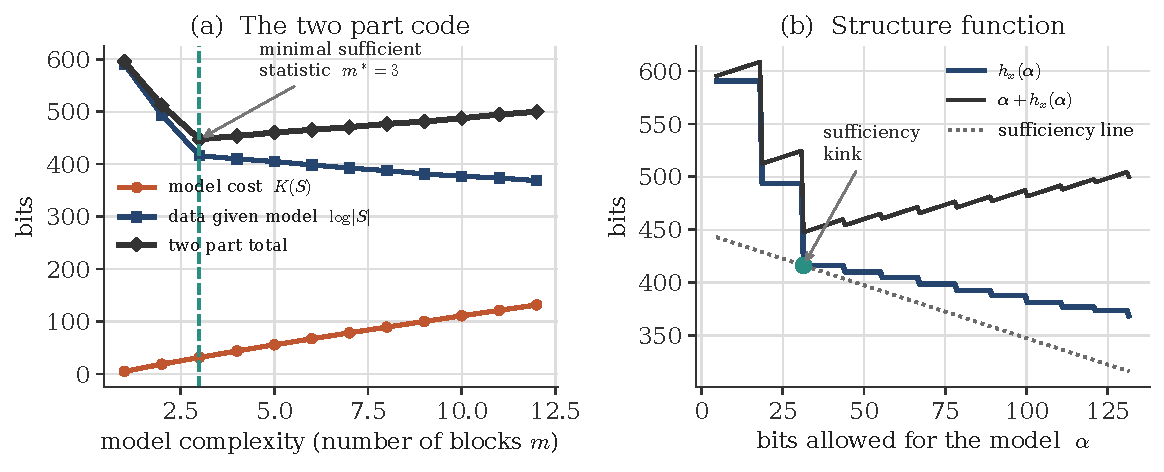
\includegraphics[width=0.9\textwidth]{app_kolmogorov}
\caption{A computable structure function over a restricted model class. A six hundred bit string is
generated from three blocks of differing bias, and models are piecewise constant descriptions with
$m$ blocks. (a) Model cost, data cost given the model, and their total, which is minimized at the
true $m^*=3$. (b) The structure function, dropping to a kink at the sufficient statistic and then
falling by about half a bit per bit of model, more slowly than the dotted sufficiency line of
slope $-1$ that the structure function over all finite sets follows from the minimal sufficient
statistic up to $\alpha=K(x)$.}
\label{fig:app_kolmogorov}
\end{figure}

\subsection{What incomputability costs, and what it does not}\label{kc:sec:incomputable}
$K$ is upper semicomputable and not computable: it can be approximated from above by running
programs and waiting, never from below, so no procedure certifies that a shortest description has
been found. It is tempting to conclude that the theory is therefore ornamental. That conclusion is
wrong in a specific and useful way. The incomputability is a statement about the universal machine,
which quantifies over all programs; restrict the model class to something a statistician would
actually write down, as in the figure above, and both parts of the code become computable, the
minimization becomes a finite search, and what survives is the two part accounting. Every
criterion of Section~\ref{ch:mdl} is such a restriction. The normalized maximum likelihood code is
the minimax optimal choice within a parametric class, the two part code is the direct analogue, and
the marginal likelihood is the Bayesian average that replaces the minimum. The ideal is not
attainable, but it is the object the attainable criteria are approximating, and that is what tells
us they are approximating the same thing.

The same reading explains the modern puzzle of Section~\ref{ch:dd}. Parameter count is not a
description length, because a model with many parameters that are heavily constrained, quantized, or
concentrated in a flat basin has a short description. Effective complexity saturates while parameter
count grows, which is what the flat stretch of the total $\alpha+h_x(\alpha)$ looks like when it is reached from
the other side. A model is entitled to as many parameters as it can compress.

\subsection{Randomness, typicality, and exchangeability}\label{kc:sec:random}
The randomness deficiency of $x$ in a model $S$ is $\delta(x\mid S)=\log|S|-K(x\mid S)$, the number
of bits by which $x$ is more compressible than a generic member of $S$. A string is typical for its
model when the deficiency is small, and a good model is one for which the data are typical. This is
the algorithmic version of the typicality that drives the method of types in
Section~\ref{ch:types}: there, typical sequences are those whose empirical distribution sits near
the generating one and whose count is $2^{nH}$; here, typicality is a property of the individual
sequence relative to a description. Sanov's theorem and the structure function are the ensemble and
the individual forms of one statement, that structure is what shortens a description and everything
else costs full price.

The connection to exchangeability is equally direct. De Finetti's theorem says an exchangeable
sequence is a mixture over parameters, which is a statement about the joint law; the algorithmic
reading says that a sequence whose complexity is explained by its type, with the arrangement within
the type incompressible, is one for which the parameter is the whole story. Both say that the order
carries no information beyond the counts, and the second says it of the particular sequence in hand.

\paragraph{Summary.} Kolmogorov complexity supplies a definition of information for a single object,
an exact notion of what a model is through algorithmic sufficiency, and a diagnostic, the structure
function, whose kink marks the point past which further modeling is wasted effort. It is
not computable, and it is not meant to be used directly; it is the standard against which the
computable criteria of the previous section are measured, and the reason they agree with one another.

\subsection*{Problems}
\begin{enumerate}[leftmargin=1.8em,itemsep=2pt]
\item Prove the invariance theorem: for universal machines $U$ and $U'$ there is a constant $c$ with $|K_U(x)-K_{U'}(x)|\le c$ for all $x$.
\item Show that at most $2^{n-k}$ strings of length $n$ have $K(x)<n-k$, so that most strings are incompressible.
\item For $x$ drawn from a computable source $P$, show that $\E[K(x)]$ and the entropy $H(P)$ differ by at most $K(P)+O(1)$.
\item Define the structure function $h_x(\alpha)$ and show that it is nonincreasing, that $h_x(\alpha)+\alpha\ge K(x)-O(1)$ for all $\alpha$, and that equality to within a constant identifies a sufficient statistic.
\item Reproduce the piecewise constant experiment of Figure~\ref{fig:app_kolmogorov} with four blocks instead of three and confirm that the two part code is minimized at the true number of blocks.
\item Explain why $K$ is upper semicomputable but not computable, and why restricting the model class to a parametric family makes both parts of the code computable.
\end{enumerate}

\src{Kolmogorov (1965) and Chaitin (1969) on complexity; Solomonoff (1964) on the universal prior;
Levin on algorithmic probability; Vereshchagin and Vit\'anyi on the structure function and algorithmic
sufficiency; Li and Vit\'anyi for the standard treatment; and Kolmogorov on Cybernetics (Polson and
Sokolov, 2026a) for the trajectory from the 1933 axioms to the algorithmic theory and its bearing on
contemporary machine learning.}


\section{Shrinkage in Pictures}\label{ch:shrinkpics}\index{shrinkage}\index{horseshoe prior}\index{James Stein estimator}\index{global local prior}

\noindent\textbf{Thesis.} Every Bayesian estimate is a shrinkage estimate: the posterior mean pulls the
data toward what the prior expected, and the entire art lies in how far and for whom. The rules
differ in one picture, the posterior mean as a function of the observation, and that picture is
decided by the prior on a single number, the fraction of the observation to discard. This section
draws the pictures before the next one proves the theorems.

\subsection{The rule is a curve}\label{sp:sec:rules}
Take one observation $y\sim\Ncal(\beta,1)$ and ask for $\E[\beta\mid y]$. With no prior
information the answer is $y$, the dotted diagonal in Figure~\ref{fig:shr_rules}(a). Every prior
bends that line toward zero, and the four priors drawn bend it in characteristically different
ways. A Gaussian prior gives ridge regression: the line is still straight, with slope one half at
unit prior variance, so a large observation is halved as a small one is. A Laplace prior
gives the Bayesian lasso: the curve is shrunk by a nearly constant amount, so the rule behaves like
soft thresholding. The Cauchy prior and the horseshoe do something the first two cannot, which panel
(b) isolates by plotting the amount shrunk. Under the Gaussian the amount shrunk grows without
bound, three units at $y=6$; under the Laplace it is a constant one unit; under the Cauchy and the
horseshoe it rises to a peak near $y=2$ and then falls back toward zero, so that a clear signal is
returned almost intact, about $0.34$ units short of $y$ at $y=6$. This is bounded influence, and it
is the property that separates a robust shrinkage rule from a merely convenient one.

\begin{figure}[H]
\centering
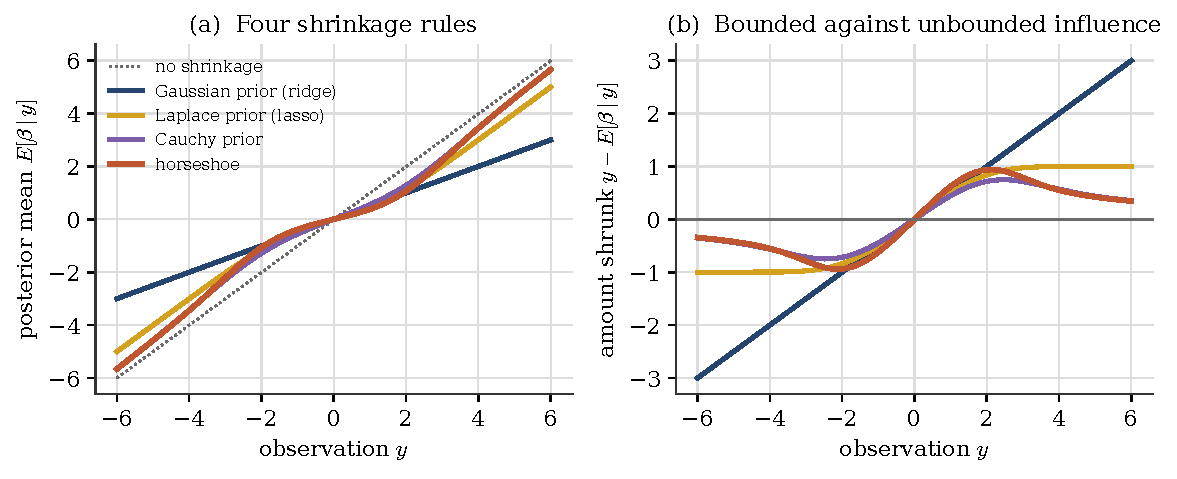
\includegraphics[width=0.92\textwidth]{shr_rules}
\caption{Four shrinkage rules for one Gaussian observation. (a) The posterior mean against the
observation, with the diagonal of no shrinkage dotted. (b) The amount shrunk. The Gaussian prior
shrinks without bound, the Laplace by a constant, and the Cauchy and horseshoe priors shrink hardest
near two and then let a large signal through nearly untouched.}
\label{fig:shr_rules}
\end{figure}

\subsection{The prior on the shrinkage weight}\label{sp:sec:kappa}
Write the local variance as $\lambda^2$ and define $\kappa=1/(1+\lambda^2)$, the fraction of the
observation thrown away, so that $\E[\beta\mid y,\lambda]=(1-\kappa)y$. Every scale mixture prior
induces a prior on $\kappa$, and Figure~\ref{fig:shr_kappa} shows that this one dimensional density
is the whole story. The horseshoe gives $\mathrm{Beta}(\tfrac12,\tfrac12)$, unbounded at both ends and
lowest in the middle, so the prior tilts toward the two decisions a sparse problem faces, shrink to
nothing or leave alone, though $0.2\le\kappa\le0.8$ still carries $41\%$ of its mass. The pole at $\kappa=1$ comes from the local scale's positive density at the
origin and delivers the sparsity; the pole at $\kappa=0$ comes from the Cauchy tail and delivers the
bounded influence of the previous figure. The Strawderman and Berger prior keeps the pole at zero but
not at one, the Laplace prior has neither and concentrates its mass in the middle, where it
shrinks everything by a similar amount, and the Student $t$ prior with three degrees of freedom sits
in between. Reading a shrinkage rule off its $\kappa$ density is faster than integrating its
posterior, and it is how the horseshoe was designed.

\begin{figure}[H]
\centering
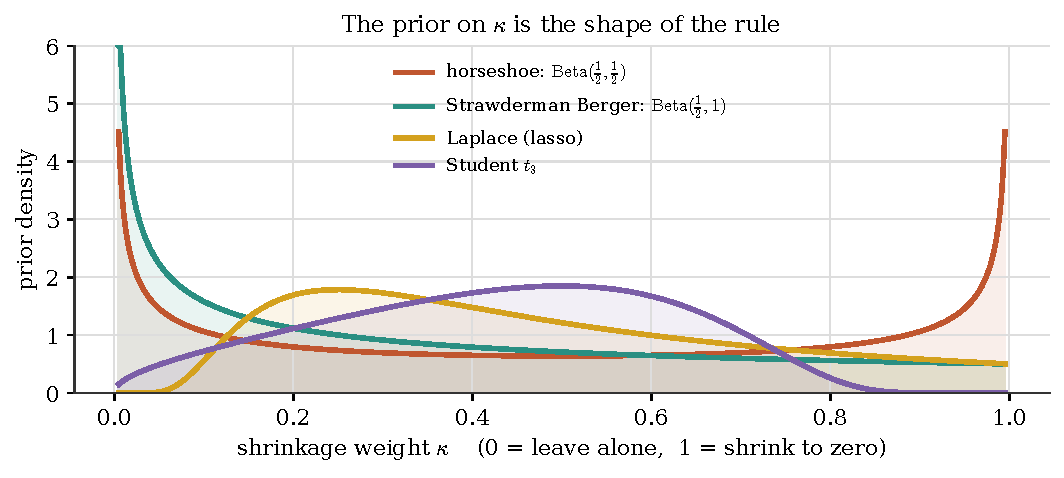
\includegraphics[width=0.85\textwidth]{shr_kappa}
\caption{The induced prior on the shrinkage weight $\kappa$ for four scale mixture priors. The
horseshoe is unbounded at both ends; mass near one produces sparsity and mass near zero produces
bounded influence. The Laplace prior has neither pole.}
\label{fig:shr_kappa}
\end{figure}

\subsection{Stein's paradox}\label{sp:sec:stein}
Shrinkage was not invented for sparsity. Stein showed in 1956 that for three or more Gaussian
means estimated simultaneously, the sample mean vector is inadmissible: the James and Stein rule
$(1-(p-2)/\|y\|^2)\,y$ has lower expected total squared error for every value of the true vector.
Figure~\ref{fig:shr_jamesstein}(a) shows the size of the effect at the origin, where the risk of the
sample mean grows linearly with the dimension while the James and Stein risk stays at two whatever
$p$ is. Panel (b) holds $p=10$ and moves the true vector away from the origin: the gain shrinks as
the signal grows but never becomes a loss, and the positive part rule, which refuses to shrink past
zero, improves on it everywhere. The lesson that carries through the rest of the book is that
simultaneous estimation is never a collection of separate problems. The coordinates share a scale,
and estimating that scale from all of them at once is what the prior does.

\begin{figure}[H]
\centering
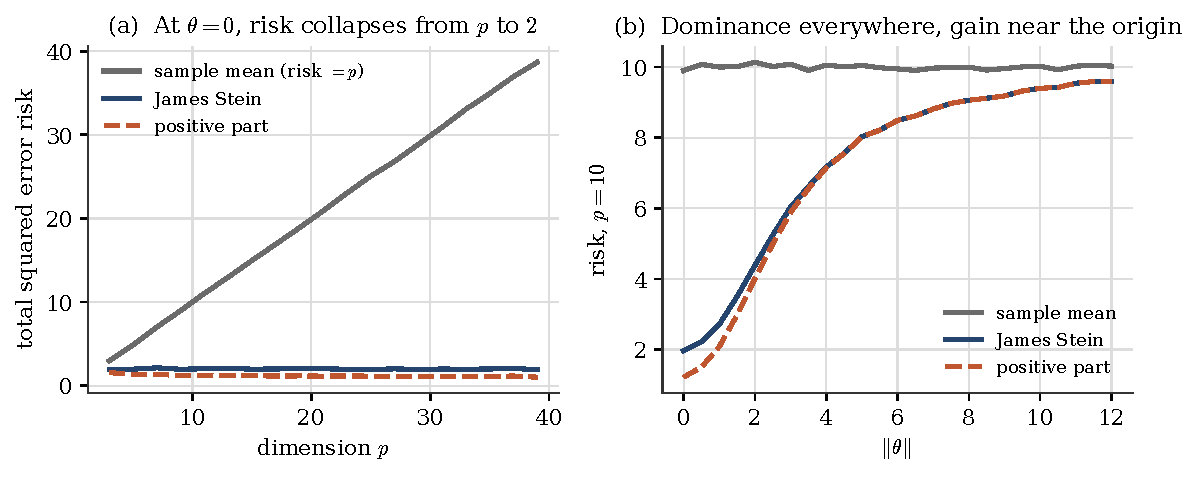
\includegraphics[width=0.92\textwidth]{shr_jamesstein}
\caption{Stein's paradox by simulation. (a) At the origin, the risk of the sample mean grows with
the dimension while the James and Stein rule holds at two. (b) At $p=10$, the gain diminishes as
the true vector moves away from the origin but never reverses; the positive part rule dominates
throughout.}
\label{fig:shr_jamesstein}
\end{figure}

\subsection{Batting averages}\label{sp:sec:baseball}
Efron and Morris made Stein's result famous with batting averages: take each player's average over
the first forty five at bats of a season and ask how well it predicts the rest. The early averages
are noisy, with a binomial standard error near $0.065$ against a spread of true abilities of perhaps
$0.03$, so most of the visible spread is noise, and the empirical Bayes rule shrinks each player
toward the grand mean by a factor estimated from the data. Figure~\ref{fig:shr_baseball} reproduces
the exercise on a synthetic season built with those magnitudes. The early averages fan out, the
shrunk estimates pull sharply toward the center, and the rest of season outcomes land close to the
shrunk values: the estimated shrinkage weight is $0.79$, and the mean squared prediction error of
the shrunk estimates is three and a half times smaller than that of the raw averages. The hot
starter is mostly lucky, the slow starter mostly unlucky, and shrinkage is the arithmetic of saying
so.

\begin{figure}[H]
\centering
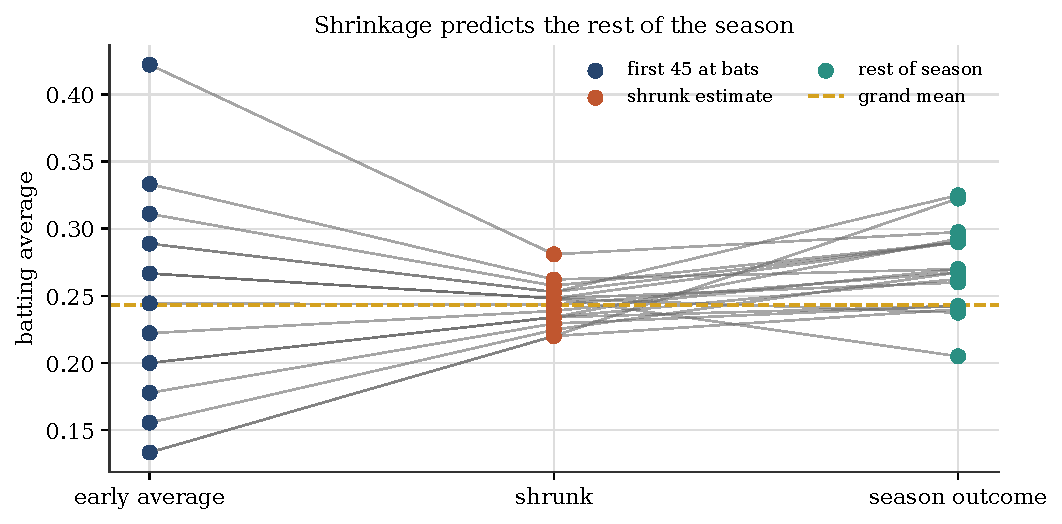
\includegraphics[width=0.85\textwidth]{shr_baseball}
\caption{Eighteen players on a synthetic season in the manner of Efron and Morris. Early averages
over forty five at bats, the empirical Bayes shrunk estimates, and the rest of season outcomes.
Shrinking toward the grand mean cuts prediction error by a factor of three and a half.}
\label{fig:shr_baseball}
\end{figure}

\subsection{Global and local}\label{sp:sec:globallocal}
The horseshoe carries two scales. The local scale $\lambda_i$ lets each coordinate escape
shrinkage on its own evidence; the global scale $\tau$ sets how much evidence is required. The
heatmap of Figure~\ref{fig:shr_globallocal} shows the fraction of the observation retained as a
function of both, with the observation across and the global scale up. Along any horizontal line
the rule is the horseshoe curve of Figure~\ref{fig:shr_rules}: the least kept for small $y$, almost
everything for large. What moves with $\tau$ is the location of the transition. At $\tau=1$ the
half retention contour sits near $y=2$; at $\tau=0.05$ it has moved out past $y=3$, and the region
of near total shrinkage has grown to cover every observation a pure noise coordinate would plausibly
produce. The global scale is therefore the sparsity dial, and because it is estimated from all
coordinates at once it is set by how many of them look like noise. The calibration section that
follows works out where it should sit on the moderate deviation scale.

\begin{figure}[H]
\centering
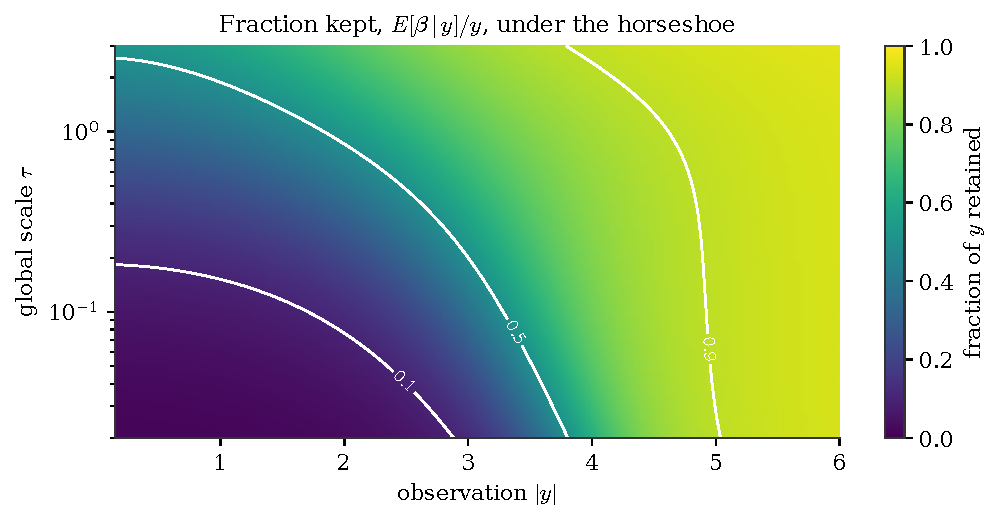
\includegraphics[width=0.85\textwidth]{shr_globallocal}
\caption{The horseshoe's two scales. Shading, from dark (none) to light (all), gives the fraction of the observation retained; white
contours mark ten, fifty and ninety percent. Lowering the global scale $\tau$ moves the transition
outward, demanding more evidence before a coordinate is believed.}
\label{fig:shr_globallocal}
\end{figure}

\subsection{Sparse recovery}\label{sp:sec:sparse}
Figure~\ref{fig:shr_sparse} puts the pieces together on two hundred coordinates, twelve of which
carry signals between three and six in absolute value and the rest nothing, each observed with unit
noise. The raw observations in panel (a) show the signals, circled, standing over a forest of noise
of typical size $0.8$. The horseshoe posterior means in panel (b), computed coordinate by
coordinate at a global scale of a quarter, flatten the forest to a typical size of $0.15$ while
leaving eleven of the twelve signals standing above every noise posterior mean in absolute value, with ninety five percent intervals. Total mean squared
error falls from $1.00$ to $0.22$. The cost is visible too, and should be stated: the signals are
pulled in by a little more than the noise alone would explain, an average absolute error of $1.2$
against $0.9$ for the raw values, and the ninety five percent intervals cover nine of the twelve signals against all $188$ noise coordinates. Both are the price of a global scale set low enough to clear the
noise. That tradeoff is what the moderate deviation calibration of the next section
resolves, by placing the global scale where the two costs balance.

\begin{figure}[H]
\centering
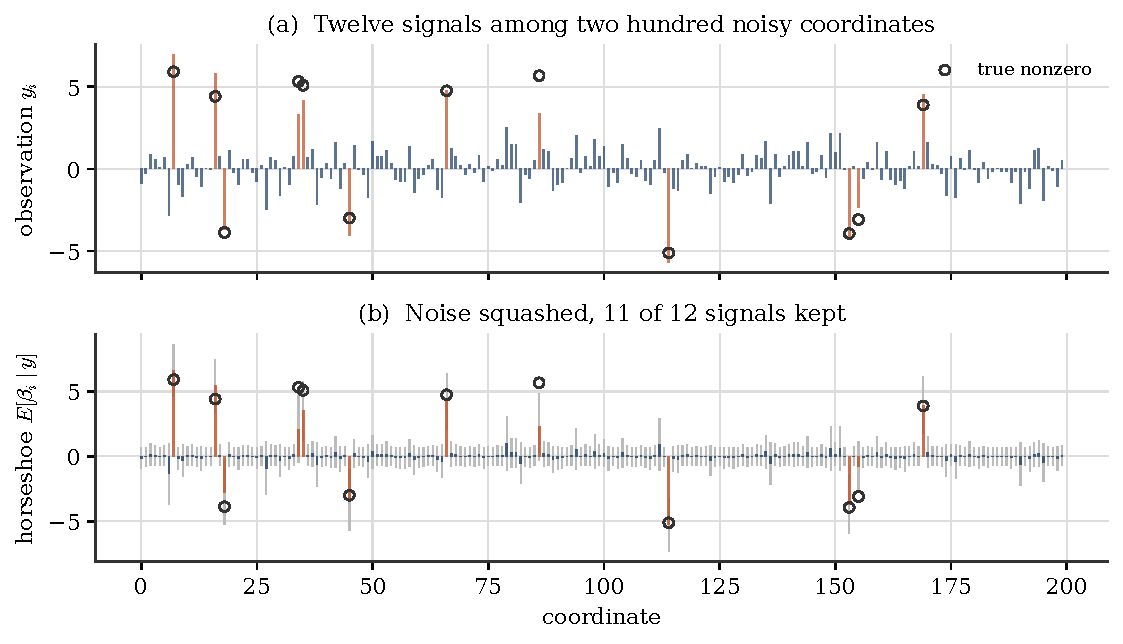
\includegraphics[width=0.92\textwidth]{shr_sparse}
\caption{Sparse recovery with the horseshoe. (a) Two hundred observations, twelve of which carry a
signal (circled). (b) Posterior means with ninety five percent intervals: noise coordinates are
flattened by a factor of five, eleven of the twelve signals are kept, and total error falls by a factor of four and a
half.}
\label{fig:shr_sparse}
\end{figure}

\paragraph{Summary.} A shrinkage rule is a curve, the curve is set by the prior on the shrinkage
weight, and two poles in that prior buy sparsity and bounded influence respectively. Stein's paradox
says simultaneous estimation always rewards shrinking toward a shared center, batting averages show
what that buys in prediction, and the global scale of a global local prior is the dial that turns a
robust rule into a sparse one.

\subsection*{Problems}
\begin{enumerate}[leftmargin=1.8em,itemsep=2pt]
\item For $y\sim\Ncal(\beta,1)$ and $\beta\sim\Ncal(0,v)$, show that $\E[\beta\mid y]=vy/(1+v)$ and that the amount shrunk is unbounded in $y$.
\item Show that under the Laplace prior $\tfrac12e^{-|\beta|}$ the posterior mean satisfies $y-\E[\beta\mid y]\to\pm1$ as $y\to\pm\infty$, and interpret this as soft thresholding.
\item Derive the $\mathrm{Beta}(\tfrac12,\tfrac12)$ law of $\kappa=1/(1+\lambda^2)$ when $\lambda$ is standard half Cauchy, and locate the two poles in the behavior of the half Cauchy density at zero and at infinity.
\item Prove that $\E[\beta\mid y]=y+\frac{d}{dy}\log m(y)$ where $m$ is the marginal density of $y$ (Tweedie's formula), and use it to explain why bounded influence is a statement about the tail of $m$.
\item Compute the risk of the James and Stein estimator at the origin and show that it equals two for every $p\ge3$.
\item Reproduce the batting average experiment with the true spread of abilities set to $0.01$ and to $0.06$, and report how the estimated shrinkage weight and the prediction gain change.
\item In the sparse recovery example, repeat the fit with the global scale at $1$ and at $0.05$ and describe what happens to the noise floor and to the signal error in each case.
\end{enumerate}

\src{Stein (1956) and James and Stein (1961); Efron and Morris (1975) on batting averages; Carvalho,
Polson and Scott (2010) on the horseshoe and the law of the shrinkage weight; Polson and Scott (2012a, 2012b)
on local shrinkage rules and the half Cauchy global scale; Strawderman (1971) and Berger (1980) on
the alternative scale mixture.}


\section[Horseshoe Priors and Moderate Deviations]{Horseshoe Priors, Moderate Deviations, and Bayes Information Theory}\label{ch:hsmdp}

\noindent\textbf{Thesis.} The two structural features of the horseshoe prior, an
infinite spike at the origin and Cauchy tails, are the finite-sample expressions
of the moderate-deviation optimality conditions for sparse testing. The
Polson--Scott log-pole and super-efficiency bounds, the moderate-deviation
threshold at the $\sqrt{\log n}$ scale, and the Clarke--Barron information-theoretic
asymptotics are three readings of one object. The log-pole is the minimal
unbounded singularity admissible at the origin among power-law mixing measures; the super-efficiency theorem is
the risk-side counterpart of the moderate-deviation threshold, both carrying a
$\log\log n$ correction; and the $\kappa$-scale, with its $\mathrm{Beta}(1/2,1/2)$
law on the shrinkage weight, encodes the transition between the shrinkage and
no-shrinkage regimes. This section is the sparse-signal instance of the deviation
ladder of Section~\ref{ch:deviations} and the information-budget accounting of
Section~\ref{ch:risk}.

\subsection{Introduction}\label{hs:sec:intro}

The horseshoe prior for sparse normal means has, since its introduction by
Carvalho, Polson and Scott (2009), been understood to possess two structural properties that set it apart
from other continuous shrinkage priors: an \emph{infinite spike at zero}, where the
marginal density $\pH(\theta)\to\infty$ as $\theta\to0$, unlike the Lasso, ridge, or
Student-$t$ priors which have bounded density at the origin (Bhadra et al., 2019); and \emph{heavy Cauchy-like
tails}, where for large $|\theta|$, $\pH(\theta)$ decays like $|\theta|^{-2}$, leaving
large signals unshrunk. These features have been exploited computationally, empirically
and theoretically, but their asymptotic interpretation in relation to hypothesis testing
and Bayes risk calibration has not been fully worked out. The purpose of this section is to
close that gap by showing that the Polson--Scott bounds are, in a precise sense, the
finite-sample expressions of the MDP optimality conditions established by
Datta, Polson, Sokolov and Zantedeschi (2026, arXiv:2602.11132).

The horseshoe prior emerged from a line of work on continuous shrinkage alternatives to
spike-and-slab priors (Mitchell and Beauchamp, 1988). The spike-and-slab prior places a point mass at
zero mixed with a continuous slab, achieving exact sparsity at substantial computational
cost in high dimensions. Carvalho, Polson and Scott (2009) proposed the horseshoe as a continuous
alternative mimicking spike-and-slab behavior through the scale-mixture representation
$\theta_i\mid\lambda_i,\tau\sim\N(0,\lambda_i^2\tau^2)$ with $\lambda_i\sim\Cp(0,1)$,
where the half-Cauchy prior on the local scale generates both the infinite spike and the
heavy tails. The Bayesian Lasso (Park and Casella, 2008), which uses a Laplace prior on $\theta_i$,
had earlier been shown to have bounded density at zero and exponential tails, leading to over-shrinkage of
large signals.

The theoretical program developed in three stages. First, Carvalho, Polson and Scott (2010) established
the tight log-pole bounds and the super-efficiency theorem for the KL risk of the Bayes
predictive. Second, Polson and Scott (2010) characterized necessary and sufficient conditions on
the prior's behavior at the origin for near-oracle risk in the sparse normal means
problem. Third, the posterior concentration theory of van der Pas, Kleijn and van der Vaart (2014) and van der Pas, Salomond and Schmidt-Hieber (2016)
established that the horseshoe achieves the minimax rate $(p_0/n)\log(n/p_0)$ for
estimating nearly black vectors, and Datta and Ghosh (2013) proved that the horseshoe achieves
asymptotic Bayes optimality under sparsity (ABOS) \emph{up to a multiplicative constant}
in the multiple testing framework of Bogdan et al.\ (2011). Further developments include the
horseshoe+ estimator (Bhadra et al., 2017), the Dirichlet--Laplace prior
(Bhattacharya et al., 2015), and the asymptotic optimality results of Ghosh and Chakrabarti (2017) for
one-group shrinkage priors. The sparsity information framework of Piironen and Vehtari (2017) provides
practical guidance on choosing the global scale $\tau$.

The MDP of Datta, Polson, Sokolov and Zantedeschi (2026) establishes that the Bayes-risk-optimal threshold for sparse
testing lies at the moderate deviation scale $\sqrt{\log n}$, intermediate between the
CLT scale $O(1)$ and the Bonferroni threshold $\sqrt{2\log n}$, and that the
exact threshold constant depends on the prior's behavior at the origin.

\paragraph{Contributions.}
\begin{enumerate}[leftmargin=1.6em,itemsep=0.25em]
\item We locate the log-pole in the power-law family $\nu(ds)\asymp s^{-\gamma}ds$ of admissible origin behaviors
(Proposition~\ref{hs:prop:levy}) and show it is the \emph{minimal} unbounded singularity in that family:
the weakest behavior at the origin satisfying the necessary condition of
Theorem~\ref{hs:thm:nec}. It is not, as sometimes stated, the strongest normalizable
singularity; by Proposition~\ref{hs:prop:orig} every $|\theta|^{-\alpha_0}$ with $\alpha_0\in(0,1)$ is
normalizable and strictly stronger (\S\ref{hs:sec:channel1}).
\item We show the super-efficiency theorem is the risk-side counterpart of the MDP
threshold. Both carry a $\log\log n$ correction: the Ces\`aro KL risk at a null coordinate
is $n^{-1}(\tfrac12\log n-\log\log n+O(1))$ against $n^{-1}(\tfrac12\log n+O(1))$ for any prior bounded and positive near the
origin, and the horseshoe testing boundary is $\log n-2\log\log n+O(1)$
(\S\ref{hs:sec:channel2}).
\item We identify the Clarke--Barron information-theoretic asymptotics as a unifying
framework (\S\ref{hs:sec:channel3}).
\item We derive the $\kappa$-scale representation and show that the
$\mathrm{Beta}(1/2,1/2)$ distribution on the shrinkage weight encodes the transition
between the shrinkage and no-shrinkage regimes (\S\ref{hs:sec:kappa}).
\end{enumerate}

\subsection{The Polson--Scott Bounds}\label{hs:sec:ps}

Polson and Scott's analysis of global-local priors turns on three sharp inequalities, which we state in turn: a tight bound on the log-pole a prior places at the origin, a super-efficiency theorem for the resulting estimator, and the conditions a density must satisfy to recover a sparse signal.

\subsubsection{The tight log-pole bounds}

The univariate horseshoe marginal density $\pH(\theta)$, obtained by integrating out the
local scale $\lambda\sim\Cp(0,1)$ in $\theta\mid\lambda,\tau\sim\N(0,\lambda^2\tau^2)$,
has no closed form. Setting $\tau=1$,
\begin{equation}\label{hs:eq:marg}
\pH(\theta)=\int_0^\infty\frac{1}{\sqrt{2\pi}\,\lambda}
\exp\!\Big(-\frac{\theta^2}{2\lambda^2}\Big)\cdot\frac{2}{\pi(1+\lambda^2)}\,d\lambda .
\end{equation}

Near $\theta=0$ the Gaussian kernel is nearly constant for $\lambda\gg|\theta|$, so the
integral is dominated by that region, where the half-Cauchy density is roughly flat for $\lambda<1$ and the integrand is $\sim\lambda^{-1}$.
The resulting $\int_{|\theta|}^1\lambda^{-1}d\lambda=\log(1/|\theta|)$ is a
logarithmic pole, not a power-law pole, because the Gaussian decay for $\lambda\ll|\theta|$ and the half-Cauchy decay
for $\lambda\gg1$ cut the integral off at both ends. For large $|\theta|$ the Gaussian
concentrates at $\lambda\approx|\theta|$ and the half-Cauchy tail dominates, giving the
$\theta^{-2}$ tail.

\begin{theorem}[Carvalho, Polson and Scott (2010)]\label{hs:thm:bounds}
Let $K=(2\pi^3)^{-1/2}$. Then $\lim_{\theta\to0}\pH(\theta)=\infty$, and for
$\theta\ne0$,
\begin{equation}\label{hs:eq:bounds}
\frac{K}{2}\log\!\Big(1+\frac{4}{\theta^2}\Big)<\pH(\theta)<
K\log\!\Big(1+\frac{2}{\theta^2}\Big).
\end{equation}
\end{theorem}

As $\theta\to0$ the upper bound behaves like $-2K\log|\theta|$ and the lower like $-K\log|\theta|$, giving
$\pH(\theta)\asymp-\log|\theta|$; as $|\theta|\to\infty$ both behave like $2K/\theta^2$.
The bounds are tight in the sense that the ratio of upper to lower converges to $2$ as
$|\theta|\to0$ and to $1$ as $|\theta|\to\infty$. These are exact two-sided inequalities,
not asymptotic approximations.

The proof substitutes $u=\lambda^{-2}$ in \eqref{hs:eq:marg}, which gives
$\pH(\theta)=K\int_0^\infty e^{-\theta^2u/2}(1+u)^{-1}du$, and bounds the factor $(1+u)^{-1}$ by
$(1-e^{-2u})/(2u)<(1+u)^{-1}<(1-e^{-u})/u$ for $u>0$. The right inequality is equivalent to $e^{u}>1+u$, and the left to $g(u)=u-1+(1+u)e^{-2u}>0$, which holds because $g(0)=0$ and $g'(u)=1-(1+2u)e^{-2u}>0$. Integrating against $e^{-\theta^2u/2}$ with Frullani's integral $\int_0^\infty(e^{-au}-e^{-bu})u^{-1}du=\log(b/a)$ for $0<a<b$ gives \eqref{hs:eq:bounds}, and the lower bound gives $\pH(\theta)\to\infty$ as $\theta\to0$.

\subsubsection{The super-efficiency theorem}\label{hs:sec:super}

Consider $y_i\mid\theta_i\sim\N(\theta_i,\sigma^2)$ and the horseshoe Bayes predictive
for a future observation $z$,
\begin{equation}\label{hs:eq:pred}
\hat f(z\mid y_i)=\int\N(z;\theta_i,\sigma^2)\,p(\theta_i\mid y_i,\tau)\,d\theta_i .
\end{equation}
When $\theta_i=0$ the true sampling density is $f_0(z)=\N(z;0,\sigma^2)$.

\begin{theorem}[Carvalho, Polson and Scott (2010), Theorem 4]\label{hs:thm:super}
Let $R_n=n^{-1}\sum_{j=1}^{n}\E\,L(p_{\theta_0},\hat p_j)$ be the Ces\`aro-average
Kullback--Leibler risk of the Bayes predictive after $j-1$ observations, for
$y_j\sim\N(\theta_0,\sigma^2)$. Under the horseshoe prior the optimal rate when
$\theta_0=0$ is
\begin{equation}\label{hs:eq:super}
R_n=n^{-1}\big(\tfrac12\log n-b\log\log n+O(1)\big),\qquad b=1,
\end{equation}
while for $\theta_0\neq0$ it is $n^{-1}(\tfrac12\log n+O(1))$. For any prior whose
density is continuous, bounded above and strictly positive near $\theta_0$, the optimal
rate is $n^{-1}(\tfrac12\log n+O(1))$ regardless of $\theta_0$.
\end{theorem}

Carvalho, Polson and Scott (2010) state the rate as $O(n^{-1}(\log n-b\log\log n))$, which as an order of magnitude cannot be told apart from $O(n^{-1}\log n)$; \eqref{hs:eq:super} is the sharp form.
The $-b\log\log n$ in \eqref{hs:eq:super} and the $-2\log\log n$ in the horseshoe threshold
\eqref{hs:eq:hsthresh} are the same correction seen twice, once in the risk and once in the
boundary ($t^2_{\mathrm{crit}}=2nR_n+O(1)$), and this is the sharpest form of the connection this section is after.
Super-efficiency here is the removal of a $\log\log n$ term, not a change of polynomial
order. The horseshoe attains $(\tfrac12\log n-\log\log n+O(1))/n$ where every prior with bounded
and positive density near the origin attains $(\tfrac12\log n+O(1))/n$; both exceed $1/n$. The gain is real but modest,
and it is driven by the prior mass a log-pole places in a Kullback--Leibler neighborhood
of the null, through Lemma~1 of Clarke and Barron (1990), $nR_n\le n\epsilon-\log\Pi(A_\epsilon)$: for $\sigma=1$, $A_\epsilon=\{|\theta|\le\sqrt{2\epsilon}\}$ and the lower bound in \eqref{hs:eq:bounds} give
$\Pi(A_\epsilon)\ge K\int_0^{\sqrt{2\epsilon}}\log(1+4\theta^{-2})\,d\theta$, and
the substitution $u=\theta^{-2}$ and one integration by parts give
$\Pi(A_\epsilon)\ge K(2\epsilon)^{1/2}\log(1+2/\epsilon)$, so that at $\epsilon=1/n$, $-\log\Pi(A_\epsilon)\le\tfrac12\log n-\log\log n+O(1)$, which is the source of the
$\log\log n$. In outline, the matching lower bound holds because $nR_n=\tfrac12\log(n/2\pi)-\tfrac12-\E_0\log m_n(\bar y)$, where $m_n$ is the marginal density of the sample mean $\bar y$, and the upper bound in \eqref{hs:eq:bounds} keeps $m_n$ below a constant multiple of $\log n$.

\begin{remark}\label{hs:rem:rate}
Theorem~\ref{hs:thm:super} gives no rate of $O(\tau^4)$, or $O(\tau^4\log^2(1/\tau))$, for a single observation at fixed
$\tau$, and so no conclusion that the
null-coordinate risk is $o(1/n)$. Its content is the
Ces\`aro average \eqref{hs:eq:super}, a rate in $n$ with no $\tau$ in it, and it exceeds
$1/n$ rather than falling below it. Direct evaluation of the fixed-$\tau$ single-observation
risk gives $\asymp\tau/\sqrt{\log(1/\tau)}$ as $\tau\to0$, which is a third quantity again. The consequence for
\eqref{hs:eq:riskdecomp} is stated there: null coordinates are cheaper than signal
coordinates by one $\log\log n$, not exempt.
\end{remark}

\subsubsection{Necessary and sufficient conditions, and the L\'evy characterization}
\label{hs:sec:ns}

\begin{theorem}[Polson and Scott (2010), necessary]\label{hs:thm:nec}
For a scale mixture prior $\pi(\theta)=\int_0^\infty\N(\theta;0,\lambda^2)g(\lambda)
d\lambda$ to achieve near-oracle risk as $n\to\infty$ under sparsity, it is necessary
that $\pi(0)=+\infty$.
\end{theorem}

\begin{theorem}[Polson and Scott (2010), sufficient]\label{hs:thm:suff}
If $\pi(\theta)\asymp-\log|\theta|$ near zero and
$\pi(\theta)\asymp|\theta|^{-\alpha_{\mathrm{tail}}}$ for some
$\alpha_{\mathrm{tail}}\in(1,2]$ in the tails, then the prior achieves near-oracle risk.
\end{theorem}

We write $\alpha_{\mathrm{tail}}$ for the tail exponent and $\alpha_0$ for the
exponent of any pole at the origin; the two carry opposite admissible ranges.

The combination of an unbounded pole at zero, but an integrable one, is the
characterization of interest. Too weak, meaning bounded density as in the Lasso or ridge,
fails Theorem~\ref{hs:thm:nec}. Too strong, meaning a power-law pole
$|\theta|^{-\alpha_0}$ with $\alpha_0\ge1$, gives a prior that is not normalizable near
the origin (Proposition~\ref{hs:prop:orig}). We call the origin behaviors between these two failures admissible: they meet the necessary condition of Theorem~\ref{hs:thm:nec} and are normalizable, but Theorem~\ref{hs:thm:suff} gives a sufficient condition at the log-pole alone. Whether the stronger admissible poles $|\theta|^{-\alpha_0}$ with $\alpha_0\in(0,1)$ also achieve near-oracle risk is not settled here.

A concrete inadmissible case is supplied by Proposition~\ref{hs:prop:levy}: taking
$\nu(ds)\asymp s^{-\gamma}ds$ with $\gamma\ge1$ gives $\pi(\theta)\asymp
|\theta|^{-(2\gamma-1)}$ with exponent at least one, which by
Proposition~\ref{hs:prop:orig} is not normalizable near the origin. The Cauchy prior on
$\theta$ is \emph{not} such an example: $\pi(0)=1/\pi<\infty$, so it fails
Theorem~\ref{hs:thm:nec} for the same reason as the Lasso, and its heavy tail is irrelevant
to the origin condition.

To see what bounded density at zero costs, consider the Laplace prior
$\pi(\theta)=(2\lambda)^{-1}e^{-|\theta|/\lambda}$, which has $\pi(0)=1/(2\lambda)<\infty$.
For a null coordinate with $\theta_i=0$ and $y_i\sim\N(0,\sigma^2)$, the shrinkage weight
$\E[\kappa_i\mid y_i]$ is bounded away from $1$ on $|y_i|\le\sigma$, but so is the horseshoe's at
any fixed $\tau$, so one observation does not separate the two priors. With $n$ observations
the Laplace prior mass $\Pi(A_{1/n})$ is of order $n^{-1/2}$, with no logarithmic factor, and
the Ces\`aro risk of Theorem~\ref{hs:thm:super} is
\begin{equation}\label{hs:eq:laplacekl}
R_n^{\mathrm{Laplace}}=n^{-1}\big(\tfrac12\log n+O(1)\big).
\end{equation}
See Proposition~\ref{hs:prop:laplace} for the precise statement; letting $\lambda$ depend on $n$ changes the prior and requires the bound to be
rederived, rather than ``reducing'' it.

Polson and Scott (2010) further characterize admissible sparse priors through their representation
as L\'evy processes. Any scale mixture $\pi(\theta)=\int_0^\infty\N(\theta;0,s)\nu(ds)$ is
characterized by its L\'evy measure $\nu$, and
\begin{equation}\label{hs:eq:pizero}
\pi(0)=\frac{1}{\sqrt{2\pi}}\int_0^\infty s^{-1/2}\nu(ds).
\end{equation}

\begin{proposition}\label{hs:prop:levy}
Let $\nu(ds)\asymp s^{-\gamma}ds$ near $s=0$, with $\int_1^\infty s^{-1/2}\nu(ds)<\infty$, so that $s\ge1$ adds a bounded term to $\pi$.
For $\nu(ds)=s^{-\gamma}ds$ on $(0,1)$, substituting $u=\theta^2/(2s)$ in the mixture representation gives
\[
\pi(\theta)\;=\;\frac{2^{\gamma-1/2}}{\sqrt{2\pi}}\,|\theta|^{1-2\gamma}
\int_{\theta^2/2}^\infty u^{\gamma-3/2}e^{-u}\,du+O(1),
\]
and as $\theta\to0$ the integral stays bounded if and only if $\gamma>1/2$, in which case it
tends to $\Gamma(\gamma-\tfrac12)$ and
\[
\pi(\theta)\;\sim\;C_\gamma\,|\theta|^{1-2\gamma},
\qquad
C_\gamma=\frac{2^{\gamma-1/2}\,\Gamma(\gamma-\tfrac12)}{\sqrt{2\pi}} .
\]
Hence, by comparison with this case, as $\theta\to0$
\[
\begin{aligned}
\gamma<\tfrac12&:\ \pi(0)<\infty;\\
\gamma=\tfrac12&:\ \pi(\theta)\asymp-\log|\theta|;\\
\gamma>\tfrac12&:\ \pi(\theta)\asymp|\theta|^{-\alpha_0},\quad\alpha_0=2\gamma-1 .
\end{aligned}
\]
Combined with Proposition~\ref{hs:prop:orig}, which requires $\alpha_0<1$ for
normalizability, the admissible window is $\gamma\in[1/2,1)$, with $\gamma=1/2$ the
logarithmic boundary.
\end{proposition}

The horseshoe sits at $\gamma=1/2$. With $\lambda\sim\Cp(0,1)$ and $s=\lambda^2$,
the induced density on the variance is
\begin{equation}\label{hs:eq:sdens}
p(s)=\frac{1}{\pi\sqrt s\,(1+s)}\;\asymp\;s^{-1/2}\quad\text{near }s=0,
\end{equation}
so by \eqref{hs:eq:pizero}, $\pi(0)\propto\int_0 s^{-1/2}\cdot s^{-1/2}ds
=\int_0 s^{-1}ds$, a logarithmic divergence. This is the mechanism producing the log-pole
of Theorem~\ref{hs:thm:bounds}. 

The horseshoe therefore sits at the left endpoint of the admissible window: it is the
least aggressive origin behavior of the family $\nu(ds)\asymp s^{-\gamma}ds$ meeting Theorem~\ref{hs:thm:nec}, with priors at
$\gamma\in(1/2,1)$ being strictly more concentrated at zero while remaining normalizable.

\subsection{The MDP Framework}\label{hs:sec:mdp}

Consider $n$ independent tests of $H_{0i}:\theta_i=0$ against $H_{1i}:\theta_i\ne0$ based
on $y_i\sim\N(\theta_i,1)$, under the two-groups model with sparsity proportion $p_0/n$.
The Bayes risk of a procedure $\varphi$ with rejection region $\{|y_i|>t_n\}$ is
\begin{equation}\label{hs:eq:bayesrisk}
r(\pi,\varphi)=(1-p_0/n)\,P_0(|Y|>t_n)+(p_0/n)\int P_\theta(|Y|\le t_n)\,d\pi(\theta).
\end{equation}

The ABOS framework of Bogdan et al.\ (2011) concerns the Bayes risk under zero--one loss,
that is the expected number of misclassified hypotheses. At the optimal threshold the
Type~I contribution per test is at most $2\phi(t)/t$. When signals come from a normal slab
whose variance grows like $\log(n/p_0)$, $t$ eventually exceeds $\sqrt{2\log(n/p_0)}$, so this
is at most $(p_0/n)\{\pi\log(n/p_0)\}^{-1/2}$, and missed signals give an oracle risk per test
of order $p_0/n$; see
Theorem~\ref{hs:thm:oracle}. This is the \emph{testing} rate, and it should not be confused
with the minimax $\ell_2$ rate $p_0\log(n/p_0)/n$ for estimating nearly black vectors
(van der Pas, Kleijn and van der Vaart, 2014), which is larger by a factor of order $\log(n/p_0)$ and governs
a different loss. Datta and Ghosh (2013) proved the
horseshoe attains the ABOS rate up to a constant. The MDP result of Datta, Polson, Sokolov and Zantedeschi (2026)
refines this by identifying the exact threshold constant.

The threshold requires care, because the horseshoe falls outside the scope of the
result usually quoted for it. The frame also changes here. In \eqref{hs:eq:bayesrisk} and \eqref{hs:eq:balance}, as in the ABOS discussion, $n$ counts tests, each based on one observation $y_i$; from \eqref{hs:eq:sourcethresh} to \eqref{hs:eq:mills}, as in Theorem~\ref{hs:thm:mdp}, $n$ is the sample size of a single test, $t_{\mathrm{crit}}$ and $t_n$ are cuts on the standardized mean $\sqrt n\,|\bar x|/\sigma$, and the number of such tests is written $m$. Datta, Polson, Sokolov and Zantedeschi (2026) assume $\pi(\theta_0)=c_\pi\in
(0,\infty)$, that is a prior density at the null that is finite \emph{and} positive, and
obtain
\begin{equation}\label{hs:eq:sourcethresh}
t^2_{\mathrm{crit}}=\log n+\log(c_\pi^{-2})-\log(2\pi\sigma^2)
+2\log(\pi_0/\pi_a)+O\big(\sqrt{(\log n)/n}\big).
\end{equation}
For the Cauchy prior $\theta\sim C(0,\sigma)$ with $\sigma=1$ and equal prior odds,
$c_\pi=1/\pi$ and \eqref{hs:eq:sourcethresh} collapses to $t^2_{\mathrm{crit}}=\log(\pi n/2)$.
That is where the constant $\pi/2$ comes from: the Cauchy normalization $1/\pi$, entering
through $\log(c_\pi^{-2})=2\log\pi$ against $-\log(2\pi)$. It has nothing to do with
$K=(2\pi^3)^{-1/2}$.

The horseshoe has $\pH(0)=+\infty$ and therefore violates the hypothesis of
\eqref{hs:eq:sourcethresh}. Datta, Polson, Sokolov and Zantedeschi (2026) treat it separately: using
$\pH(\theta)\asymp\log(1+1/\theta^2)$ near the origin, for $|\bar x|=O(\sigma\sqrt{(\log n)/n})$,
\begin{equation}\label{hs:eq:hsbf}
\log\mathrm{BF}_{01}=\tfrac12\log n-\log\log n+O(1)-\frac{n\bar x^2}{2\sigma^2},
\end{equation}
so that the horseshoe rejection boundary is
\begin{equation}\label{hs:eq:hsthresh}
t^2_{\mathrm{crit}}=\log n-2\log\log n+O(1).
\end{equation}

This is the correct connection between the log-pole and the MDP threshold, and it is
a sharper one than a constant. An unbounded density at the null dilutes evidence more
aggressively than a finite one, so the boundary is \emph{lowered} by $2\log\log n$ for the log-pole, relative
to the $\pi(\theta_0)\in(0,\infty)$ case. The log-pole does not select a multiplicative
constant in the threshold; it produces a second-order logarithmic correction. The rate
$\sqrt{\log n}$ is unchanged, consistent with the universality in
\eqref{hs:eq:sourcethresh}.

\begin{theorem}[Datta, Polson, Sokolov and Zantedeschi (2026), Thm.~4.1]\label{hs:thm:mdp}
Let $\bar X_n\sim\N(\theta,\sigma^2/n)$ with $\sigma$ known, and test $H_0:\theta=0$
against $H_a:\theta\neq0$. Suppose the prior under $H_a$ is $C^3$ with at most polynomial
growth and $\pi(0)=c_\pi\in(0,\infty)$. Under $0$--$1$ loss with prior weights
$\pi_0,\pi_a>0$, the risk-optimal boundary satisfies \eqref{hs:eq:sourcethresh}. The leading
term $\log n$ is universal across regular models and priors; the additive constants depend
on $c_\pi$, the Fisher information and the prior model odds.
\end{theorem}

The boundary lies in the moderate deviation regime, between the CLT scale $O(1)$, where
tail probabilities do not decay, and the large deviation scale, where they decay
exponentially. At the moderate deviation scale they decay polynomially, and it is this
polynomial decay that balances against the $n^{-1/2}$ arising from integrating the
alternative. The Mills ratio approximation for the normal tail is
\begin{equation}\label{hs:eq:mills}
P_0(|Y|>t_n)\approx\frac{2\phi(t_n)}{t_n}
=\frac{\sqrt{2/\pi}}{t_n}\exp(-t_n^2/2)\asymp\frac{1}{\sqrt{n\log n}},
\end{equation}
which multiplied by $(1-p_0/m)\approx1$ and summed over $m$ tests of $n$ observations each gives total Type~I
error $O(m/\sqrt{n\log n})$.

The Bayes-optimal threshold balances Type~I and Type~II errors. Differentiating
\eqref{hs:eq:bayesrisk},
\begin{equation}\label{hs:eq:balance}
\frac{\partial}{\partial t_n}r(\pi,\varphi)=0
\iff
(1-p_0/n)\cdot2\phi(t_n)
=(p_0/n)\int\!\big[\phi(t_n-\theta)+\phi(t_n+\theta)\big]d\pi(\theta),
\end{equation}
the right side being $2(p_0/n)(\phi*\pi)(t_n)$ for $\pi$ symmetric. Under a local approximation
of the convolution by $\pi(t_n)$, valid when $\pi$ varies slowly on the unit scale, this is $\approx2(p_0/n)\pi(t_n)\int\phi(u)du=2(p_0/n)\pi(t_n)$.

The rate $\sqrt{\log n}$ is determined by the balance between the Gaussian tail decay
$e^{-t^2/2}$ and the number of tests, independent of the prior. The constant depends on the
prior density at the threshold. This separation of rate and constant is characteristic of
moderate deviation theory: the rate comes from the exponential tilting, the constant from
the pre-exponential factor.

Two conditions must be kept apart. The Cram\'er condition of
Datta, Polson, Sokolov and Zantedeschi (2026) is a condition on the \emph{sampling} distribution: the
cumulant generating function $\psi(t)=\log\E[e^{tX_1}]$ exists in a neighborhood of the
origin. It says nothing about the prior. The condition on the prior is their
Assumption~2: $\pi\in C^3$, $\pi(\theta_0)\in(0,\infty)$, and at most polynomial growth.

The horseshoe satisfies neither the classical Cram\'er condition on its own tails,
as Remark~\ref{hs:rem:cramer} records, nor the prior regularity Assumption~2, since
$\pH(0)=+\infty$. It is not at a ``Cram\'er boundary'' in either sense. What the log-pole
does is place the horseshoe just outside the regime in which \eqref{hs:eq:sourcethresh}
holds, which is why it acquires the separate treatment leading to \eqref{hs:eq:hsthresh}. The
useful statement is about \emph{prior regularity at the null}, not Cram\'er regularity, and
the horseshoe sits at its boundary from the wrong side: among the priors with $\nu(ds)\asymp s^{-\gamma}ds$ of Proposition~\ref{hs:prop:levy} it is the weakest violation of
$\pi(\theta_0)<\infty$, diverging only logarithmically.

\subsection{Connecting the Polson--Scott Bounds to the MDP}\label{hs:sec:connect}

These bounds are not isolated facts; each is a channel through which the shrinkage geometry meets the moderate-deviation principle. We trace three: the log-pole as the boundary condition at the origin, super-efficiency as moderate-deviation detection, and the Clarke--Barron logarithmic term as the coding face of the same rate.

\subsubsection{Channel 1: the log-pole as the origin boundary}\label{hs:sec:channel1}

\begin{proposition}[origin integrability]\label{hs:prop:orig}
Consider scale mixture priors with $\pi(\theta)\sim|\theta|^{-\alpha_0}
(-\log|\theta|)^{\beta}$ as $\theta\to0$, for $\alpha_0\ge0$, $\beta\ge0$. The prior is
normalizable near the origin, $\int_0^\epsilon\pi(\theta)d\theta<\infty$, if and only if
$\alpha_0<1$. When $\alpha_0<1$ the near-zero contribution to the second moment
$\int_0^\epsilon\theta^2\pi(\theta)d\theta$ is also finite for all $\beta$.
\end{proposition}

\begin{proof}
Normalizability requires $\int_0^\epsilon\theta^{-\alpha_0}(-\log\theta)^\beta d\theta
<\infty$, which holds iff $\alpha_0<1$, the logarithmic factor being slowly varying. When
$\alpha_0<1$ the second-moment integrand is $\theta^{2-\alpha_0}(-\log\theta)^\beta$ with
$2-\alpha_0>1>0$, so it converges.
\end{proof}

\begin{remark}\label{hs:rem:cramer}
The horseshoe's global variance $\int_{-\infty}^{\infty}\theta^2\pH(\theta)d\theta$ is
infinite, because the tail $\pH(\theta)\asymp2K/\theta^2$ makes
$\int_1^\infty\theta^2\cdot\theta^{-2}d\theta$ diverge. The horseshoe therefore does not
satisfy the classical Cram\'er condition. The MDP analysis of \eqref{hs:eq:balance} depends on the prior's local
behavior near the testing boundary $|\theta|\sim\sqrt{\log n}$, where the horseshoe
density is $O(1/\log n)$ and well behaved. The infinite global variance is a feature: it
is the $1/\theta^2$ tail that leaves signals above the threshold unshrunk.
\end{remark}

Verifying the near-zero second moment for the horseshoe using the upper bound in
\eqref{hs:eq:bounds},
\begin{equation}\label{hs:eq:secondmom}
\int_0^\epsilon\theta^2 K\log\!\Big(1+\frac{2}{\theta^2}\Big)d\theta
\le K\int_0^\epsilon\theta^2\{\log3+2\log(1/\theta)\}\,d\theta<\infty,
\end{equation}
for $\epsilon\le1$, since $\theta^2(-\log\theta)\to0$ as $\theta\to0$.

By Proposition~\ref{hs:prop:levy} the log-pole is the \emph{minimal} unbounded
singularity of the family $\nu(ds)\asymp s^{-\gamma}ds$: the weakest origin behavior satisfying Theorem~\ref{hs:thm:nec}. It is not the
strongest normalizable one. By Proposition~\ref{hs:prop:orig} every $|\theta|^{-\alpha_0}$
with $\alpha_0\in(0,1)$ is normalizable, has finite near-zero second moment, and is
strictly stronger than $-\log|\theta|$. Correspondingly, the log-pole is not the
\emph{unique} singularity level satisfying both constraints; the whole window
$\gamma\in[1/2,1)$ of Proposition~\ref{hs:prop:levy} does. What distinguishes the horseshoe
is that it is the least aggressive member of that window.

\subsubsection{Channel 2: super-efficiency and the MDP detection zone}\label{hs:sec:channel2}

Theorem~\ref{hs:thm:super} and the MDP threshold together partition the line. Below the
threshold the horseshoe treats coordinates as null, and at a true null, $\theta_i=0$, super-efficiency applies, with
Ces\`aro KL risk $n^{-1}(\tfrac12\log n-\log\log n+O(1))$, below the
$n^{-1}(\tfrac12\log n+O(1))$ available to any prior bounded and positive near the origin. Above it the horseshoe
leaves signals unshrunk
through tail robustness, with $\hat\theta_i\approx y_i$ for $|y_i|\gg\tcrit$ and KL risk
at the parametric rate.

This partition follows from the log-pole bound. For $|y_i|\ll\tcrit$ the posterior
concentrates near zero because $\pH(0)=+\infty$ dominates the likelihood, giving
$\kappa_i\approx1$. For $|y_i|\gg\tcrit$ the Cauchy-like tail prevents excessive
shrinkage, giving $\kappa_i\approx0$.

The threshold does not coincide with equipoise on the shrinkage scale, that is with
$\E[\kappa_i\mid y_i=\tcrit,\tau]=1/2$. Direct evaluation of
\eqref{hs:eq:kpost} at $|y_i|=\tcrit$ from \eqref{hs:eq:hsthresh}, with the $O(1)$ term set to $0$ so that
$\tcrit^2=\log n-2\log\log n$, gives a posterior mean of $\kappa_i$ close to one, not to one half: for
$(n,\tau)=(10^3,n^{-1/2})$, $(10^4,10/n)$ and $(10^6,10^{-5})$ one finds
$\E[\kappa_i\mid y_i]=0.964$, $0.998$ and $0.9999$ respectively. The solution of
$\E[\kappa_i\mid y_i]=1/2$ sits well above the threshold, at $|y_i|=4.00$, $4.58$ and
$5.10$ for $\tau=10^{-2},10^{-3},10^{-4}$, against $\sqrt{2\log(1/\tau)}=3.03$, $3.72$
and $4.29$. The first comparison places the boundary \eqref{hs:eq:hsthresh} of a single test, whose $n$ is a sample size, on one observation $y_i$ of the normal means model with $\sigma=1$ and $\tau$ tied to $n$, so it sets the two frames of \S\ref{hs:sec:mdp} side by side rather than computing within one; the second stays within the normal means model. The qualitative partition into a shrinkage and a no-shrinkage region is
unaffected, but $\kappa_i=1/2$ is not the boundary and should not be used to define it.

Theorem~\ref{hs:thm:super} gives the rate \eqref{hs:eq:super} only at $\theta=0$, a $\pH$-null set, and $O(n^{-1}\log n)$ at each fixed $\theta\neq0$, however small. The decomposition below treats every coordinate under the threshold as null, so it is a heuristic, not a consequence of the theorem. Writing the risk decomposition over the two regions,
\begin{equation}\label{hs:eq:riskdecomp}
\begin{split}
r(\pH,\mathrm{HS})&=\underbrace{\int_{|\theta|<\tcrit}
n^{-1}\big(\tfrac12\log n-\log\log n+O(1)\big)\,d\pH(\theta)}
_{\text{super-efficient region}}\\
&\quad+\underbrace{\int_{|\theta|>\tcrit}n^{-1}\big(\tfrac12\log n+O(1)\big)\,d\pH(\theta)}_{\text{signal region}} .
\end{split}
\end{equation}
Null coordinates are cheaper than signal coordinates but not free: each contributes
$(\tfrac12\log n-\log\log n+O(1))/n$ rather than nothing. The budget language should be read in that
weaker sense, as a $\log\log n$ discount on the per-coordinate cost, not as an exemption.

\subsubsection{Channel 3: Clarke--Barron and the logarithmic budget}\label{hs:sec:channel3}

\begin{theorem}[Clarke and Barron (1990)]\label{hs:thm:cb}
For a $d$-dimensional regular parametric family with prior $\pi$ continuous and strictly positive
at $\theta_0$, the cumulative KL risk of the Bayes predictive satisfies
$\sum_{i=1}^n\E[\D{P_{\theta_0}}{\hat P_i}]=\tfrac d2\log n+O(1)$.
\end{theorem}

The route through Clarke--Barron is the one Carvalho, Polson and Scott (2010) take, and it goes through the
prior mass $\Pi(A_\epsilon)$ in a Kullback--Leibler neighborhood of $\theta_0$, not
through the self-information $-\log\pi(\theta_0)$. That distinction matters: $\Pi(A_\epsilon)$
is finite for a log-pole, and it is what Lemma~1 of Clarke and Barron (1990) requires, whereas
$-\log\pH(0)=-\infty$ and cannot be inserted into an expansion that presumes a density
bounded near $\theta_0$. Stated through the prior mass, the channel is sound and yields
the upper bound in \eqref{hs:eq:super} directly.

\begin{remark}[Attribution]
The cumulative-risk expansion of Theorem~\ref{hs:thm:cb} is usually credited to
Clarke and Barron (1990), but the $\tfrac{d}{2}\log n$ information-risk asymptotics
for the Bayes predictive density were also developed in Polson (1988) as part of a study of the
cumulative Kullback--Leibler risk of predictive densities. We state it in the Clarke--Barron form because that is the
form Carvalho, Polson and Scott (2010) invoke.
\end{remark}

\subsection{The $\kappa$-Scale}\label{hs:sec:kappa}

The horseshoe induces a $\mathrm{Beta}(1/2,1/2)$ distribution on $\kappa_i$ at $\tau=1$.
In this subsection the prior variance is scaled by the noise variance, $\theta_i\mid\lambda_i,\tau\sim\N(0,\sigma^2\lambda_i^2\tau^2)$, which is the horseshoe scale mixture of this section when $\sigma=1$, so that $\kappa_i=1/(1+\lambda_i^2\tau^2)$ is the shrinkage weight, $\E[\theta_i\mid y_i,\lambda_i,\tau]=(1-\kappa_i)\,y_i$.
Applying $\kappa=1/(1+\lambda^2\tau^2)$ to $p(\lambda)=2/(\pi(1+\lambda^2))$ with
$|d\lambda/d\kappa|=\tfrac{1}{2\tau}\kappa^{-3/2}(1-\kappa)^{-1/2}$,
\begin{equation}\label{hs:eq:kprior}
p(\kappa)=\frac{2}{\pi(1+(1-\kappa)/(\kappa\tau^2))}\cdot
\frac{\kappa^{-3/2}(1-\kappa)^{-1/2}}{2\tau}
=\frac{\tau\,\kappa^{-1/2}(1-\kappa)^{-1/2}}{\pi(1-\kappa+\kappa\tau^2)},
\end{equation}
which reduces at $\tau=1$ to $\pi^{-1}\kappa^{-1/2}(1-\kappa)^{-1/2}$, the
$\mathrm{Beta}(1/2,1/2)$ or arcsine density. For general $\tau$ the induced prior is not
Beta. This is the horseshoe-shaped density that gives the prior its name: unbounded
density near both $\kappa=0$ and $\kappa=1$, with a minimum at $\kappa=1/2$ where
$p(1/2)=2/\pi$. The mass is one; it is the density that is unbounded.

Near $\kappa_i=1$ (total shrinkage, null coordinates) the density behaves like
$(1-\kappa_i)^{-1/2}$, the $\kappa$-scale translation of the log-pole. Near $\kappa_i=0$
(no shrinkage, signals) it behaves like $\kappa_i^{-1/2}$, the translation of the heavy
tail.

The posterior on $\kappa_i$ clarifies the partition. Since
$y\mid\kappa\sim\N(0,\sigma^2/\kappa)$ when $\theta_i\mid\lambda_i,\tau\sim\N(0,\sigma^2\lambda_i^2\tau^2)$, the likelihood contributes
$\kappa^{1/2}\exp(-y^2\kappa/2\sigma^2)$, and with \eqref{hs:eq:kprior},
\begin{equation}\label{hs:eq:kpost}
p(\kappa_i\mid y_i,\tau)\;\propto\;
\frac{(1-\kappa_i)^{-1/2}}{1-\kappa_i+\kappa_i\tau^2}
\exp\!\Big(-\frac{y_i^2\kappa_i}{2\sigma^2}\Big).
\end{equation}

For large $|y_i|$ the exponential sharply penalizes $\kappa_i$ near $1$, so the posterior
concentrates near $\kappa_i=0$. For small $|y_i|$ the exponential is nearly flat and the
prior's pole at $\kappa_i=1$ dominates. The crossover occurs at
$y_i^2/(2\sigma^2)\approx\log(1/\tau)\approx\log(n/p_0)$, that is at
$|y_i|\approx\sigma\sqrt{2\log(n/p_0)}$.

The posterior on $\kappa_i$ is not maximally diffuse at the threshold. Evaluating
\eqref{hs:eq:kpost} with $\sigma=1$ at $|y_i|=\tcrit$, with the $O(1)$ term of \eqref{hs:eq:hsthresh} set to $0$ and the boundary of a single test placed on one observation as in \S\ref{hs:sec:channel2}, gives $\Var[\kappa_i\mid y_i]=0.016$, $0.010$, $0.006$
and $0.0011$ for $(n,\tau)=(10^3,n^{-1/2})$, $(10^4,10^{-2})$, $(10^3,10^{-2})$ and
$(10^4,10^{-3})$, all far below the prior variance $1/8$ of the
$\mathrm{Beta}(1/2,1/2)$ and far below the $1/4$ attainable on $[0,1]$. The posterior
concentrates near $\kappa_i=1$ at the threshold, consistent with the values of
$\E[\kappa_i\mid y_i]$ reported in \S\ref{hs:sec:channel2}.

\subsection{ABOS Theory and the Horseshoe+ Prior}\label{hs:sec:abos}

Asymptotic Bayes optimality under sparsity is the yardstick by which a shrinkage prior is judged. We recall the oracle Bayes risk that sets the target, state the optimality property, and show where the horseshoe+ stands against it.

\subsubsection{Oracle Bayes risk}\label{hs:sec:oracle}

\begin{theorem}[Bogdan et al.\ (2011), oracle Bayes risk]\label{hs:thm:oracle}
In the sparse normal means model $y_i\mid\theta_i\sim\N(\theta_i,1)$, $i=1,\dots,n$, let the
$\theta_i$ be independent, equal to $0$ with probability $1-p_0/n$ and drawn from
$\N(0,\omega_n^2)$ otherwise, with $p_0=o(n)$ and $2\log(n/p_0)/\omega_n^2\to C\in(0,\infty)$.
Then the oracle Bayes risk per test under zero-one
loss satisfies
\begin{equation}\label{hs:eq:oracle}
\Rstar=\frac{p_0}{n}\cdot\bigl(2\Phi(\sqrt C)-1\bigr)\cdot(1+o(1)).
\end{equation}
\end{theorem}

This is the testing rate; it differs from the minimax $\ell_2$ estimation rate
$p_0\log(n/p_0)/n$ by a factor asymptotic to $L/(2\Phi(\sqrt C)-1)$ with $L=\log(n/p_0)$,
which is of order $L$. The testing rate is smaller, reflecting that binary classification
is easier than point estimation.

\subsubsection{The ABOS property}

A rule $\delta_n$ is ABOS if $R_n(\delta_n)/\Rstar\to1$ as $n\to\infty$ with $p_0=o(n)$.

Datta and Ghosh (2013) prove that the horseshoe attains the oracle Bayes risk \emph{up to a
multiplicative constant}. That is weaker than ABOS in the sense just defined, which
requires the ratio to converge to one: by their result the
horseshoe is rate-optimal with a bounded constant. Ghosh and Chakrabarti (2017) later proved exact ABOS: the tests induced by horseshoe-type priors, the horseshoe among them, attain the oracle risk up to the correct constant when $\tau$ is proportional to the true proportion of alternatives.

For the Type~I error, under the horseshoe with $\tau_n\asymp p_0/n$ the posterior signal
probability crosses $1/2$ at a point $t_n>\sqrt{2\log(1/\tau_n)}$ (\S\ref{hs:sec:channel2}), so
$\alpha_n^{HS}=P(|Y_i|>t_n\mid\theta_i=0)<\tau_n/\sqrt{\pi\log(1/\tau_n)}=o(\Rstar)$, and missed
signals dominate the risk. For signals of fixed strength
$\mu_n=A\sqrt{2\log(n/p_0)}$ with $A>1$, a model outside Theorem~\ref{hs:thm:oracle}, the Type~II error is
$\beta_n^{HS}=\Phi((1-A+o(1))\sqrt{2\log(n/p_0)})$.

The connection to the Donoho and Johnstone (1994) universal threshold $\sqrt{2\log n}$ is direct: when
$p_0=O(1)$, $\sqrt{2\log(n/p_0)}$ reduces to it.

\subsubsection{The horseshoe+ prior}\label{hs:sec:hsplus}

The horseshoe+ prior (Bhadra et al., 2017) adds a second layer of half-Cauchy mixing,
\begin{equation}\label{hs:eq:hsplus}
\theta_i\mid\lambda_i,\tau\sim\N(0,\lambda_i^2\tau^2),
\qquad\lambda_i\mid\eta_i\sim\Cp(0,\eta_i),
\qquad\eta_i\sim\Cp(0,1),
\end{equation}
which strengthens the pole at the origin.

The horseshoe+ shrinkage density is not obtained by multiplying the horseshoe's
$\mathrm{Beta}(1/2,1/2)$ by a further factor $\kappa^{-1/2}(1-\kappa)^{-1/2}$; that product
is $\kappa^{-1}(1-\kappa)^{-1}$, which is not integrable on $(0,1)$, and Table~1 of
Carvalho, Polson and Scott (2010) identifies it as the normal-Jeffreys prior, the improper limit of
$\kappa\sim\mathrm{Beta}(\epsilon,\epsilon)$ as $\epsilon\to0$. The two are distinct priors.
Bhadra et al.\ (2017) obtain the horseshoe+ marginal through the
class of Meijer-$G$ functions rather than in elementary closed form, and their optimality
statement is of the same kind as the one used here for the horseshoe: the optimal Bayes
risk in testing is attained up to a constant.

\begin{table}[h]
\centering\small
\begin{tabular}{lll}
\toprule
Property & Horseshoe & Horseshoe+ \\
\midrule
Optimal $\tau_n$ & $\asymp p_0/n$ & $\asymp p_0/n$ (same) \\
KL bound at $\theta_0=0$, $\log\log n$ term & $-n^{-1}\log\log n$ & $-2n^{-1}\log\log n$ \\
\bottomrule
\end{tabular}
\caption{Horseshoe and horseshoe+ for sparse testing. The last row is the $\log\log n$ term in the upper bounds of Bhadra et al.\ (2017) on the Ces\`aro KL risk at $\theta_0=0$, a comparison of bounds, not of risks; see \S\ref{hs:sec:hsplus}.}
\label{hs:tab:hsplus}
\end{table}

\subsection{Calibration of the Global Shrinkage Parameter}\label{hs:sec:tau}

The ABOS results assume $\tau_n\asymp p_0/n$, but $p_0$ is unknown. The testing problem is
more fragile to $\tau$ miscalibration than estimation, because decisions are hard
thresholds rather than smooth shrinkage functions.

\subsubsection{Constrained marginal maximum likelihood}

The MMLE maximizes the marginal likelihood over $\tau\in[1/n,1]$. The constraint is
essential: without it the Tiao--Tan phenomenon (Tiao and Tan, 1965) causes the unconstrained
MLE to collapse to $\tau=0$ with positive probability. The lower bound corresponds to at
least one signal, the upper bound to at most all coordinates being signals.

\begin{theorem}[van der Pas, Szab\'o and van der Vaart (2017a)]\label{hs:thm:mmle}
For $p_0\to\infty$ with $p_0=o(n)$ and some constant $C$, the constrained MMLE satisfies $\hat\tau_{\mathrm{MMLE}}\in[1/n,C\tau_n(p_0)]$, where $\tau_n(p_0)=(p_0/n)\sqrt{\log(n/p_0)}$, with
probability tending to one, uniformly over the set $\ell_0[p_0]$ of vectors $\theta_0$ with at most $p_0$ nonzero coordinates.
\end{theorem}

\subsubsection{Truncated half-Cauchy prior}

The recommended fully Bayesian specification is $\tau\sim\Cp(0,1)\cdot
\mathbf{1}[\tau\in[1/n,1]]$, the half-Cauchy truncated to the range of the MMLE. Truncation prevents mass on $\tau>1$ and avoids HMC
pathologies from heavy right tails.

\begin{theorem}[van der Pas, Szab\'o and van der Vaart (2017a)]\label{hs:thm:trunc}
Under the half-Cauchy prior truncated to $[1/n,1]$, and with $C\log n\le p_0=o(n)$ for a large enough constant $C$, the horseshoe posterior contracts adaptively
at the near-minimax rate $p_0\log n/n$, against the minimax rate $p_0\log(n/p_0)/n$.
\end{theorem}

A flat prior $\tau\sim\mathrm{Unif}(0,1)$ places sufficient mass near
$\tau_0\asymp p_0/n$ for adaptive contraction in estimation, but provides no
regularization toward the sparse region, so the posterior can develop a heavy right tail
when large noise observations mimic signals, inflating Type~I error.

\subsubsection{Three regimes of inefficiency}

In the over-shrinkage regime ($\hat\tau\ll\tau_0$) the effective threshold exceeds
$t_n$ and true signals are missed; risk is dominated by Type~II error. In the
under-shrinkage regime ($\hat\tau\gg\tau_0$) the threshold drops and null observations
are falsely declared signals. At the detection boundary $\mu_n=\pm t_n$,
\begin{equation}\label{hs:eq:boundary}
R_n\ge(p_0/n)\Phi(0)=p_0/(2n)\qquad\text{when }\mu_n=t_n .
\end{equation}
This bound is conditional on $\mu_n=t_n$; that fixed signal strength lies
outside the slab model of Theorem~\ref{hs:thm:oracle}, so the bound is not a floor on
$\Rstar$. The self-similarity condition of van der Pas, Szab\'o and van der Vaart (2017b) excludes this
worst case, so the inefficiency is not irreducible within that class.

\subsection{Connection to Statistical Sparsity}\label{hs:sec:sparsity}

McCullagh and Polson (2018) define statistical sparsity through the exceedance measure: in the sparse
limit $\rho\to0$, the signal-plus-noise convolution depends on the signal distribution
only through its exceedance measure $H$ and rate $\rho$. For the horseshoe the signal
distribution in the sparse limit belongs to the class of inverse-power measures,
$H_{HS}(x,\infty)=C_\alpha/x^\alpha$ with $\alpha=1$, since the tail $2K\tau/\theta^2$ of the horseshoe density at scale $\tau$ integrates to $2K\tau/x$, and $\rho\asymp\tau\asymp
p_0/n$.

Two implications. First, any two sparse families with the same exceedance measure are
inferentially equivalent to first order in $\rho$. Second, the threshold
$\sqrt{2\log(1/\rho)}=\sqrt{2\log(n/p_0)}$ arises as the scale at which the exceedance
integral transitions from Type~I to Type~II dominated behavior. This is the threshold for
$n$ simultaneous tests, the counterpart of the threshold \eqref{hs:eq:hsthresh} for a single test.

\paragraph{Sparse factor model extension.}

The analysis is expected to extend to $Y=\Lambda F+\varepsilon$ with $\Lambda\in\mathbb R^{p\times k}$
sparse. Testing $\lambda_{ij}=0$ reduces to simultaneous testing over the $k\times p$
entries of $\Lambda$, with ABOS expected to hold conditionally on identifiability of the sparsity
pattern; following Sturma et al.\ (2025), identifiability requires a matching criterion on the
bipartite graph of nonzero loadings.

Writing $\Lambda=(\lambda_{ij})$, the testing problem ranges over all $kp$ entries, so the
risk decomposes as a sum over $(i,j)\in\{1,\dots,p\}\times\{1,\dots,k\}$ rather than over
the $k$ factors alone,
\[
R^{\mathrm{factor}}_n=\sum_{i=1}^{p}\sum_{j=1}^{k}
\big\{2\pi_{0,ij}\{1-\Phi(t_n)\}+\pi_{1,ij}\,\beta_{n,ij}\big\},
\]
each term expected to obey the same moderate deviation scaling as in the univariate case.

\subsection{Numerical Evidence}\label{hs:sec:sim}

The computation below bears directly on Theorem~\ref{hs:thm:super}.
Its mechanism is the prior mass $\Pi(A_\epsilon)$ that a log-pole places in a
Kullback--Leibler neighborhood of the null, entering the risk bound of Clarke and Barron (1990)
through $-n^{-1}\log\Pi(A_\epsilon)$ at $\epsilon=1/(2n)$. Comparing the horseshoe with a
Laplace prior $\tfrac12e^{-|\theta|}$, which is bounded at the origin, on $|\theta|\le n^{-1/2}$ (the horseshoe column takes the mass there of the lower bound $\tfrac K2\log(1+4/\theta^2)$ of Theorem~\ref{hs:thm:bounds}, a lower bound on the horseshoe mass and the side the Clarke--Barron bound needs; the Laplace column takes the exact mass $1-e^{-n^{-1/2}}$):

\begin{center}\small
\begin{tabular}{rrrrr}
\toprule
$n$ & $-\log\Pi_{HS}$ & $-\log\Pi_{\mathrm{Lap}}$ & gap & $\log\log n$\\
\midrule
$10^3$ & 3.186 & 3.470 & $-0.284$ & 1.933\\
$10^4$ & 4.135 & 4.610 & $-0.475$ & 2.220\\
$10^5$ & 5.119 & 5.758 & $-0.639$ & 2.443\\
$10^6$ & 6.126 & 6.908 & $-0.782$ & 2.626\\
$10^8$ & 8.192 & 9.210 & $-1.019$ & 2.913\\
\bottomrule
\end{tabular}
\end{center}

Regressing the gap on $\log\log n$ gives slope $-0.750$; the local slope is $-0.84$ at $n=10^8$ and tends to $-1$, since the horseshoe column is $\tfrac12\log n-\log\log n+O(1)$ and the Laplace column $\tfrac12\log n+O(1)$. The log-pole's advantage over a
bounded prior is therefore one $\log\log n$ up to a constant, which is the $b$ in
\eqref{hs:eq:super} and confirms the mechanism rather than merely the rate.

\subsection{Hierarchy of Bounds}\label{hs:sec:hier}

From most local to most global. The levels are related bounds, not a chain of implications.

\paragraph{Level 1, density bound (Theorem~\ref{hs:thm:bounds}).}
$\tfrac K2\log(1+4/\theta^2)<\pH(\theta)<K\log(1+2/\theta^2)$. The root of the hierarchy.

\paragraph{Level 2, shrinkage weight.}
For fixed $y_i$ as $\tau\to0$, \eqref{hs:eq:kpost} gives $1-\E[\kappa_i\mid y_i,\tau]\sim(\tau/\pi)\int_0^1s^{-1/2}e^{y_i^2s/(2\sigma^2)}\,ds$, of order $\tau$, so
$\hat\theta_i=O(\tau)$; as $|y_i|\to\infty$, $\E[\kappa_i\mid y_i,\tau]\sim2\sigma^2/y_i^2$ and $\hat\theta_i\approx y_i-2\sigma^2/y_i$.

\paragraph{Level 3, KL risk (super-efficiency).}
$R_n=n^{-1}(\tfrac12\log n-\log\log n+O(1))$ at $\theta_0=0$, against $n^{-1}(\tfrac12\log n+O(1))$
otherwise.

\paragraph{Level 4, Hellinger.}
$\dH^2(f_0,\hat f)\le\D{f_0}{\hat f}$. Under the convention
$\dH^2=1-\mathrm{BC}$, the leading term for two normals of common variance is
$\hat\theta_i^2/(8\sigma^2)$, an equality rather than a consequence of Level 3; under
$\dH^2=2(1-\mathrm{BC})$ it is $\hat\theta_i^2/(4\sigma^2)$. 

\paragraph{Level 5, testing boundary.}
See \eqref{hs:eq:hsthresh}: $\tcrit^2=\log n-2\log\log n+O(1)$.

\paragraph{Level 6, Type I error at the threshold.}
Uses \eqref{hs:eq:sourcethresh}. Under $\tcrit=\sqrt{\log(\pi n/2)}$ the tail is
$2/(\pi\sqrt n\,\tcrit)=O(n^{-1/2})$.

\paragraph{Level 7, ABOS Bayes risk.}
$\Rstar\asymp p_0/n$, from Theorem~\ref{hs:thm:oracle}.

\paragraph{Level 8, Clarke--Barron budget.}
Stated through the prior mass; see \S\ref{hs:sec:channel3}.

\begin{table}[h]
\centering\small
\begin{tabular}{@{}lll@{}}
\toprule
Result & Expression & MDP interpretation \\
\midrule
Log-pole density & $\pH(\theta)\asymp K\log(1/\theta^2)$
 & Minimal unbounded singularity \\
Cauchy tail & $\pH(\theta)\asymp2K/\theta^2$
 & Signals above threshold unshrunk \\
Necessary condition & $\pi(0)=+\infty$ & Required for near-oracle risk \\
Sufficient condition & log-pole $+$ heavy tail & The admissible pair \\
Super-efficiency & $n^{-1}(\tfrac12\log n-\log\log n)$ & One $\log\log n$ below a bounded prior \\
Shrinkage weight & $\kappa_i\sim\mathrm{Beta}(1/2,1/2)$ at $\tau=1$
 & Transition from $\kappa=1$ to $\kappa=0$ \\
L\'evy measure & $\nu(ds)\asymp s^{-1/2}ds$ & Logarithmic boundary, $\gamma=1/2$ \\
\bottomrule
\end{tabular}
\caption{Correspondences. The risk row follows \eqref{hs:eq:super}, and the minimality of the log-pole holds within the family $\nu(ds)\asymp s^{-\gamma}ds$ of Proposition~\ref{hs:prop:levy}.}
\label{hs:tab:corr}
\end{table}

\subsection{Discussion}\label{hs:sec:disc}

Every element of the theory involves $\log n$ or $\log(1/\theta)$. The
Rubin and Sethuraman (1965a, 1965b) theory of Bayes risk efficiency established that the moderate deviation
scale is the natural home of Bayes risk efficiency, and the horseshoe's log-pole is the
prior design that makes this scale manifest.

The comparison with other priors is instructive. The Lasso prior has bounded density at
zero and fails Theorem~\ref{hs:thm:nec}.

\begin{proposition}\label{hs:prop:laplace}
Fix a prior whose density is continuous and strictly positive at $0$, such as the Laplace
prior. Then the null-coordinate Ces\`aro KL risk of Theorem~\ref{hs:thm:super} is
$n^{-1}(\tfrac12\log n+O(1))$, with no $\log\log n$ correction.
\end{proposition}

\begin{proof}
The Ces\`aro risk is $n^{-1}$ times the cumulative risk
$\sum_{j=1}^{n}\E[\D{f_0}{\hat p_j}]$, which Theorem~\ref{hs:thm:cb} with $d=1$ and
$\theta_0=0$ evaluates as $\tfrac12\log n+O(1)$.
\end{proof}

The argument is for a fixed prior. If the scale is allowed to depend on $n$, the
prior changes with $n$ and the bound must be rederived for the resulting sequence; that
case is not covered here. 

The ridge prior fails Theorem~\ref{hs:thm:nec} for the same reason and performs worse in
sparse settings. The Student-$t$ prior with $\nu>2$ has bounded density at zero, so it is
robust but not super-efficient.

These results suggest a design principle: a sparse prior should have log-pole density at
zero and Cauchy-class tails. The log-pole gives super-efficiency for null coordinates
below the threshold; the tails give robustness (signals above it are unshrunk), a
bounded influence function, and regular variation. By
Proposition~\ref{hs:prop:levy} the admissible origin behaviors with $\nu(ds)\asymp s^{-\gamma}ds$ form the window
$\gamma\in[1/2,1)$, and the horseshoe is its left endpoint rather than its unique
member.

The log-pole principle is expected to extend to structured sparsity: group sparsity, graphical model
edge selection, and low-rank estimation, where the prior on each singular value plays the
analogous role. The conjectured general principle is that MDP-optimal inference requires an unbounded density
along whatever zero manifold defines the sparse structure.

Theoretical optimality comes with a computational cost. The log-pole creates a funnel
geometry in $(\theta_i,\lambda_i)$ that standard Gibbs samplers traverse slowly
(Neal, 2003; Piironen and Vehtari, 2017). Slice samplers and HMC with mass matrix adaptation partially address this.

Several questions remain open. The super-efficiency result assumes $\theta_i=0$ exactly,
and the KL risk when $\theta_i$ is small but nonzero is uncharacterized uniformly in $\theta_i$. In
high-dimensional regression with correlated design the effective observation for
coefficient $j$ is $\hat\beta_j^{\mathrm{OLS}}\sim\N(\beta_j,(X^\top X)^{-1}_{jj})$, and
the coordinate-wise MDP framework applies only for orthogonal designs. The ABOS framework
connects to Benjamini--Hochberg FDR control and to the multiple testing literature
(Efron, 2004; Johnstone and Silverman, 2004).

To summarize the position the horseshoe occupies. Within the one-parameter family $\nu(ds)\asymp s^{-\gamma}ds$, Proposition~\ref{hs:prop:levy} places the
admissible origin behaviors at
$\gamma\in[1/2,1)$, bounded below by the necessary condition $\pi(0)=+\infty$ and above by
normalizability. The horseshoe sits at the left endpoint $\gamma=1/2$. It is therefore not
the unique admissible prior, as the whole window qualifies, but it is the least aggressive
member of it: the weakest singularity at the origin in that family that still meets
Theorem~\ref{hs:thm:nec}, and the only member at which Theorem~\ref{hs:thm:suff} establishes near-oracle risk. It also fails the classical Cram\'er condition, its variance being
infinite, and fails the prior regularity $\pi(\theta_0)\in(0,\infty)$ required by
Theorem~\ref{hs:thm:mdp}, which is why it acquires the separate boundary
\eqref{hs:eq:hsthresh}.

What that minimality buys is a single logarithmic order, and it appears twice. In the
risk, Theorem~\ref{hs:thm:super} gives $n^{-1}(\tfrac12\log n-\log\log n+O(1))$ against $n^{-1}(\tfrac12\log n+O(1))$ for
any prior bounded and positive near the origin. In the testing boundary, \eqref{hs:eq:hsthresh} gives
$\log n-2\log\log n$ against the $\log n+O(1)$ of \eqref{hs:eq:sourcethresh}. The same
$\log\log n$ correction, once in the risk and once in the threshold, is the substance of
the connection between the Polson--Scott bounds and the moderate deviation framework. The
log-pole produces it, by enlarging the
prior mass $\Pi(A_\epsilon)$ near the null; the Cauchy tail has the complementary role of leaving signals above the boundary
unshrunk.

%%---- incorporated: non-regular models -------------------------------
\subsection{Non-Regular Models: the Ibragimov--Has'minskii Spectrum}
\label{sec:nonregular}

The moderate-deviation account above assumed a regular likelihood: the Gaussian
normal-means model, where the score is linear and the local experiment is
Gaussian. The ABOS property, the log-pole, and the $\sqrt{2\log n}$ threshold all
rest on that regularity. This section removes it. Working through the exponential
power family $f(x;\theta)=C(\beta)\exp(-|x-\theta|^\beta)$, which sweeps the entire
Ibragimov--Has'minskii taxonomy as $\beta$ runs from $0$ to $\infty$, regular for
$\beta>\tfrac12$ (with a mild cusp in the density when $\beta<1$), a cusp for $\beta\in(0,\tfrac12)$, a jump in the limit $\beta\to\infty$, we
set out an ABOS theory across the spectrum, much of it conjectural, a family of $\beta$-horseshoe
priors conjectured to achieve exact ABOS for every $\beta<2$, and a sharp phase transition at
$\beta=\tfrac12$, where the Fisher information becomes infinite and the rate leaves
$\sqrt n$. The $\beta=2$ likelihood is Gaussian, so
the regular theory of the preceding sections is one slice of what follows, although the ordinary horseshoe is not a $\beta$-horseshoe: given $\tau$ its marginal is unbounded at the origin, while every EP density is bounded there. A normal scale mixture with a positive $(\beta/2)$-stable mixing law yields a
\emph{symmetric-stable} marginal; the exponential-power family instead requires a polynomially
tilted stable mixing law (West, 1987), which is the representation that ties it to the horseshoe
hierarchy.

\subsubsection{Background}
%%=============================================================

\paragraph{The ABOS Framework}

We observe $y_i\mid\theta_i\sim p(\cdot\mid\theta_i)$, $i=1,\ldots,n$,
where $\theta=(\theta_1,\ldots,\theta_n)$ is sparse. Write
$s_n=\abs{\{i:\theta_i\neq 0\}}$ for the number of true signals and
$\pin=s_n/n$ for the sparsity proportion. The \emph{Bayes oracle} under
0--1 additive loss minimizes
\[
 \BRn(t)=\pin\,\beta_n(t)+(1-\pin)\,\alpha_n(t),
\]
where $\alpha_n(t)$ and $\beta_n(t)$ are the Type~I and Type~II error
probabilities of a fixed-threshold rule with threshold $t$. Following
Bogdan et al.\ (2011) we consider, for $\N(\theta_i,1)$ observations, the asymptotic regime $\pin\to 0$ and
$\mun\to\infty$, with nonzero $\theta_i$ drawn from $\N(0,\mun^2)$ and $2\log(1/\pin)/\mun^2\to C\in(0,\infty)$.

As in \S\ref{hs:sec:abos}, a testing rule with Bayes risk $\BRn^*$ is ABOS if
$\BRn^*/\BRn^{\mathrm{oracle}}\to 1$ as $n\to\infty$.

Datta and Ghosh (2013) proved that the horseshoe rule, reject $H_{0i}$ if
$1-\hat\kappa_i>1/2$, is ABOS up to a multiplicative constant in the
Gaussian sequence model with $\mun\asymp\sqrt{2\log n}$ and
$\tau\asymp\pin$. Ghosh and Chakrabarti (2017) later showed that horseshoe-type priors
achieve exact ABOS (ratio converging to~1) when $\tau$ is
proportional to the true proportion of alternatives.

\paragraph{The Ibragimov--Has'minskii Framework}

Let $X_1,\ldots,X_n\iid f(x;\theta)$. The \emph{normalized likelihood
ratio process} is
\[
 Z_n(u)=\prod_{i=1}^n
 \frac{f\!\left(X_i;\,\theta_0+u/\psin\right)}{f(X_i;\,\theta_0)},
 \qquad u\in\R,
\]
where $\psin$ is the normalizing rate. Under IH conditions,
$Z_n(\cdot)\toL Z(\cdot)$ as a process, where $Z$ is the
\emph{limiting likelihood ratio process} whose structure governs the
asymptotics of all reasonable estimators and tests.

The posterior in the rescaled coordinate $u=\psin(\theta-\theta_0)$,
under any prior $\pi(\theta)$ positive and continuous at $\theta_0$,
converges weakly to the \emph{random posterior density}
\[
 \Pi_\infty(du)=\frac{Z(u)}{\int Z(v)\,dv}\,du,
\]
established by Ghosh, Ghosal and Samanta (1994); Ghosal, Ghosh and Samanta (1995). Crucially, this limiting
posterior is \emph{prior-free}.

\paragraph{IH classification.}
Table~\ref{nr:tab:IH} summarizes the three canonical singularity types for
location families $f(x;\theta)=g(x-\theta)$.

\begin{table}[h]
\centering
\caption{IH classification of non-regular location models.}
\label{nr:tab:IH}
\renewcommand{\arraystretch}{1.3}
\small\setlength{\tabcolsep}{5pt}
\begin{tabular}{@{}llll@{}}
\toprule
Type & Singularity & Rate $\psin$ & Limiting process $Z(u)$ \\
\midrule
Type~0 (LAN) & $g$ smooth, $\Info(\theta)<\infty$ & $n^{1/2}$
 & $\exp(uW-u^2/2)$, $W\sim\N(0,1)$ \\
Type~1 (Jump) & $g$ has jump at~$0$ & $n$
 & Exponential/Poisson functional \\
Type~2 (Cusp, $\alpha<\tfrac12$) & $g(0)-g(x)\sim c|x|^\alpha$
 & $n^{1/(2\alpha+1)}$ & Fractional Brownian functional \\
\bottomrule
\end{tabular}
\end{table}

\paragraph{The Exponential Power Family}

The EP$(\beta)$ location family is
\[
 f(x;\theta)=\frac{\beta}{2\,\Gamma(1/\beta)}
 \exp\!\bigl(-|x-\theta|^\beta\bigr),\quad x\in\R,\ \beta>0.
\]
It admits the \emph{scale mixture of normals} representation
\[
 f(x;\theta)=\int_0^\infty \N(x;\theta,\sigma^2)\,
 p(\sigma^2;\beta)\,d\sigma^2,
\]
where $p(\sigma^2;\beta)$ is the law of the reciprocal of a polynomially tilted positive $(\beta/2)$-stable variable
(West, 1987; Polson, 1988). The IH regime is:
\begin{itemize}
 \item $\beta>\tfrac12$: Type~0 (LAN), rate $\psin=n^{1/2}$,
 $\Info(\theta)=\beta^2\,\Gamma\!\left((2\beta-1)/\beta\right)/
 \Gamma(1/\beta)<\infty$.
 \item $\beta=\tfrac12$: LAN, but the Fisher information is infinite and the rate is $\psin=(n\log n)^{1/2}$.
 \item $\beta\in(0,\tfrac12)$: Type~2 (cusp), rate $\psin=n^{p(\beta)}$
 where
 \[
 p(\beta)=\frac{1}{2\beta+1}\in\Bigl(\tfrac{1}{2},1\Bigr).
 \]
 \item $\beta\to\infty$: approaches Type~1 (jump), rate $\psin=n$.
\end{itemize}
The function $p(\beta)$ is strictly decreasing with
$p(\beta)\to 1$ as $\beta\to 0$ and $p(\beta)\to\tfrac{1}{2}$ as
$\beta\to\tfrac12$. For $\beta\ge\tfrac12$ we set $p(\beta)=\tfrac12$, ignoring the factor $\sqrt{\log n}$ at $\beta=\tfrac12$; the Fisher information, of order $\beta$ for large $\beta$, grows without bound, so the rate $n$ belongs to the uniform limit only.

%%=============================================================
\subsubsection{The Bayes-Risk MDP Principle in Non-Regular Models}
%%=============================================================

\paragraph{Three Deviation Regimes}

In $\psin$-scaled coordinates $T_n^{(p)}=\psin(\thetahat-\theta_0)$, with $\thetahat$ the MLE, $\lambda_n>0$ a level for the deviation $|\thetahat-\theta_0|$ and $t_n=\psin\lambda_n$ the matching threshold for $|T_n^{(p)}|$,
three deviation regimes arise:
\begin{description}
 \item[CLT scale:] $t_n=O(1)$. Type~I error $\alpha_n=O(1)$.
 \item[MDP scale:] $t_n^{1/p}\asymp\log n$, that is $t_n\asymp(\log n)^p$, which at the LAN rate $p=\tfrac12$ is $\psin^2\lambda_n^2\asymp\log n$, giving
 $t_n\asymp\sqrt{\log n}$ in rescaled coordinates. Both error
 probabilities decay polynomially, because for each type in Table~\ref{nr:tab:IH} the squared Hellinger distance between $\theta_0$ and $\theta_0+\lambda_n$ is of order $\lambda_n^{1/p}$, and $n\lambda_n^{1/p}=t_n^{1/p}$.
 \item[LDP scale:] $\lambda_n=O(1)$ but large. Exponential decay
 (Chernoff exponents).
\end{description}

\begin{conjecture}[MDP Principle for IH Models]
\label{nr:thm:mdp}
Let the IH model have posterior concentration rate $n^p$ with $p=\tfrac12$ and limiting
LR process $Z(u)$, and suppose the limiting Bayes factor $\int Z(u)\,du$ has null tail
$\Prob(\int Z(u)\,du>t)=t^{-\gamma_p+o(1)}$ for some $\gamma_p\ge1$.
Under symmetric $0$--$1$ loss and a prior $\pi(\theta)$ positive and
smooth at $\theta_0$, the Bayes-risk-optimal threshold in
$n^p$-scaled coordinates satisfies
\[
 \tcrit^{(p)}=\sqrt{\gamma_p\log n}+o(\sqrt{\log n}),
\]
and both Type~I and~II Bayes risks decay as $n^{-\gamma_p/2+o(1)}$.
In the original $\theta$ scale:
\[
 |\theta|_{\mathrm{crit}}=n^{-p}\sqrt{\gamma_p\log n}.
\]
\end{conjecture}

\begin{remark}[Recovery of the threshold of Datta et al.]
For the regular case ($p=\tfrac{1}{2}$, Gaussian LR
process, $\int Z(u)\,du=\sqrt{2\pi}\,e^{W^2/2}$, so $\gamma_p=1$), Conjecture~\ref{nr:thm:mdp} gives
$\tcrit=\sqrt{\log n}$ in $\sqrt{n}$-scaled coordinates, the leading term of the
result $\tcrit=\sqrt{\log(\pi n/2)}$ of Datta, Polson, Sokolov and Zantedeschi (2026) for the Cauchy prior (Theorem~\ref{hs:thm:mdp}).
\end{remark}

\paragraph{The Phase Transition at $\beta=\tfrac{1}{2}$}

For EP$(\beta)$ with $\beta\ge\tfrac12$ the model is LAN (at rate $\sqrt n$, or $\sqrt{n\log n}$ at $\beta=\tfrac12$), so its limiting LR process is the Gaussian one of the regular case after a rescaling of $u$, and the tail exponent takes the regular value
\[
 \gamma_p(\beta)=1,\qquad \beta\ge\tfrac{1}{2}.
\]
The \emph{phase transition} at $\beta=\tfrac12$ is a change of rate and, below it, of the limiting process:

\begin{itemize}
 \item $\beta\ge\tfrac{1}{2}$: Conjecture~\ref{nr:thm:mdp} would give the regular threshold
 $\tcrit^{(p)}=\sqrt{\log n}$ in the LAN-scaled coordinates.
 \item $\beta<\tfrac{1}{2}$: the rate is $n^{1/(2\beta+1)}$ and the limiting LR process is the fractional Brownian one of Table~\ref{nr:tab:IH}; its exponent $\gamma_p$, and with it the optimal threshold, is not derived here.
\end{itemize}

%%=============================================================
\subsubsection{ABOS Theory for the IH Spectrum}
%%=============================================================

\paragraph{The Three Load-Bearing Pillars of ABOS}

The Datta and Ghosh (2013) ABOS proof rests on three conditions.

\medskip
\noindent\textbf{Pillar~1} (Normal likelihood).
The model $y_i\mid\theta_i\sim\N(\theta_i,1)$ gives the posterior a
normal-mixture structure enabling the shrinkage weight $\kappa_i$ to
separate signals from nulls cleanly.

\medskip
\noindent\textbf{Pillar~2} (Posterior bimodal concentration).
At signal strength $\mun\asymp\sqrt{2\log n}$:
\begin{align*}
 \theta_i=0\;(\text{null})\;&\Longrightarrow\;
 \E[\kappa_i\mid y_i]\to 1\;(\text{full shrinkage}),\\
 |\theta_i|\ge\mun\;(\text{signal})\;&\Longrightarrow\;
 \E[\kappa_i\mid y_i]\to 0\;(\text{no shrinkage}).
\end{align*}

\medskip
\noindent\textbf{Pillar~3} (Cram\'er MDP tail probability).
Under $H_0$,
$\Prob(|y_i|>\mun)\sim 2\phi(\mun)/\mun=O(n^{-1}/\sqrt{\log n})$,
giving Type~I contribution $O(n^{-1})$ per test.

\paragraph{Case~1: Mild Cusp, $\beta\in(\tfrac{1}{2},1)$}
\label{nr:sec:mildcusp}

Pillar~1 is violated but the scale-mixture representation
$f(x;\theta)=\int\N(x;\theta,\sigma^2)p(\sigma^2;\beta)\,d\sigma^2$
preserves tractability. The model is LAN in this range ($p=\tfrac12$, $\gamma_p=1$), and Pillars~2 and~3 are conjectured to hold with modifications, the
bimodal separation occurring at the modified signal strength
$\mun=n^{-p}\sqrt{(2/\beta)\log n}$.

\begin{conjecture}[Modified ABOS for mild cusp]
\label{nr:prop:mildcusp}
For \textup{EP}$(\beta)$ with $\beta\in(\tfrac{1}{2},1)$, sparsity
$\pin\to 0$, and
$\mun=n^{-p}\sqrt{(2/\beta)\log n}$, the horseshoe with
$\tau\asymp\pin$ satisfies
\[
 1\;\le\;\limsup_{n\to\infty}
 \frac{\BRn^{\mathrm{horseshoe}}}{\BRn^{\mathrm{oracle}}}
 \;\le\;\frac{2}{\beta}.
\]
\end{conjecture}

If the conjecture holds, the horseshoe is \emph{conservative}: its Cauchy tails are more than
sufficient to detect signals at the oracle scale, so ABOS holds up to
the constant $2/\beta>2$.

\paragraph{Case~2: Horseshoe Boundary, $\beta=\tfrac{1}{2}$}

At $\beta=\tfrac{1}{2}$ the EP mixing law is that of the reciprocal of a polynomially tilted positive $(\tfrac14)$-stable variable,
not the L\'evy, or $(\tfrac12)$-stable, law, and not the half-Cauchy mixing of the standard
horseshoe, which is not a stable law. The
limiting LR process is Gaussian, as in the regular case ($\gamma_p=1$), but at the rate
$\sqrt{n\log n}$, because the Fisher information is infinite.

How the Type~I and Type~II error rates balance at this boundary is not
derived here.

\begin{conjecture}[Weak ABOS at the boundary]
\label{nr:prop:boundary}
At $\beta=\tfrac{1}{2}$, the horseshoe achieves
$\BRn^{\mathrm{horseshoe}}=O(\BRn^{\mathrm{oracle}})$, but exact ABOS
fails: there exists $C_*\in(1,\infty)$ such that
\[
 \limsup_{n\to\infty}
 \frac{\BRn^{\mathrm{horseshoe}}}{\BRn^{\mathrm{oracle}}}=C_*.
\]
\end{conjecture}

\paragraph{Case~3: Strong Cusp, $\beta<\tfrac{1}{2}$}

For $\beta<\tfrac{1}{2}$ the rate is $n^p$ with $p=1/(2\beta+1)>\tfrac12$, and the
limiting LR process is the fractional Brownian one of Table~\ref{nr:tab:IH}; its
exponent $\gamma_p$ and the Bayes-risk-optimal threshold are not derived here.
The posterior concentrates at the scale $n^{-p}$, finer than the regular MDP scale
$n^{-1/2}\sqrt{\log n}$ at which the horseshoe, calibrated to the $\sqrt n$ rate,
is expected to threshold.

\begin{conjecture}[ABOS failure for strong cusp]
\label{nr:prop:strongcusp}
For \textup{EP}$(\beta)$ with $\beta<\tfrac{1}{2}$,
\[
 \liminf_{n\to\infty}
 \frac{\BRn^{\mathrm{horseshoe}}}{\BRn^{\mathrm{oracle}}}=\infty.
\]
\end{conjecture}

\paragraph{Case~4: Jump Discontinuity (IH Type~1)}

For a jump at the edge of the support, say a density that rises from $0$ to $1/\gamma$ there, as for the shifted exponential with scale $\gamma$, the posterior is a shifted exponential in
$n$-scaled coordinates. The oracle threshold is
$|\theta|_{\mathrm{crit}}=(\gamma/n)\log n$ in original $\theta$ scale, smaller than the
horseshoe threshold $n^{-1/2}\sqrt{\log n}$ by a factor of order
$\sqrt{n/\log n}\to\infty$.

\begin{conjecture}[Complete ABOS failure for jump models]
\label{nr:prop:jump}
For IH Type~$1$ (jump-discontinuity) models, the horseshoe Bayes risk
diverges relative to the oracle both asymptotically and at finite
samples. No member of the $\beta$-horseshoe family (for finite $\beta$)
achieves ABOS in this regime.
\end{conjecture}

Table~\ref{nr:tab:abos} summarizes the four cases.

\begin{table}[h]
\centering
\caption{ABOS status across the IH spectrum. The rates $p$ are established, with an extra factor $\sqrt{\log n}$ at $\beta=\tfrac12$; the ABOS and fix entries for $\beta\in(0,1)$ and for the jump are conjectures.}
\label{nr:tab:abos}
\renewcommand{\arraystretch}{1.3}
\setlength{\tabcolsep}{5pt}
\begin{tabular}{@{}lcccc@{}}
\toprule
Regime & $\beta$ & Rate $p$ & ABOS & Fix \\
\midrule
Regular (LAN) & $\ge1$ & $\tfrac{1}{2}$ & Exact & -- \\
Mild cusp & $(\tfrac{1}{2},1)$ & $\tfrac{1}{2}$
 & Up to $\tfrac{2}{\beta}$ & $\beta$-HS recovers exact \\
Boundary & $\tfrac{1}{2}$ & $\tfrac{1}{2}$
 & Weak only & $\tfrac{1}{2}$-HS (boundary) \\
Strong cusp & $(0,\tfrac{1}{2})$ & $(\tfrac{1}{2},1)$
 & Fails & $\beta$-HS \\
Jump (Type~1) & $\to\infty$ & $1$ & Completely fails
 & Exponential posterior geometry \\
\bottomrule
\end{tabular}
\end{table}

%%=============================================================
\subsubsection{Generalized Horseshoe Priors}
%%=============================================================

\paragraph{The $\beta$-Horseshoe}

\begin{definition}[$\beta$-Horseshoe Prior]
For $\beta\in(0,2]$, the \emph{$\beta$-horseshoe prior} on $\theta_i$ is
\[
 \theta_i\mid\lambdai,\tau\sim\N(0,\lambdai^2\tau^2),\qquad
 \lambdai^2\sim p(\cdot\,;\beta),\qquad
 \tau\sim\Stable\!\left(\tfrac{\beta}{2},1,\pin,0\right),
\]
where $p(\cdot\,;\beta)$ is the mixing law of the EP$(\beta)$ representation above, the law of the reciprocal of a polynomially tilted positive $(\beta/2)$-stable variable, and $\Stable(\alpha,\beta_0,\gamma,\delta)$ denotes the stable
distribution with index $\alpha$, skewness $\beta_0$, scale $\gamma$,
and shift $\delta$.
\end{definition}

The marginal of $\theta_i$ given $\tau$ under the $\beta$-horseshoe is
EP$(\beta)$:
\[
 p(\theta_i)=\frac{\beta}{2\tau\,\Gamma(1/\beta)}
 \exp\!\bigl(-|\theta_i/\tau|^\beta\bigr),
\]
matching the tail structure of the EP$(\beta)$ likelihood.

\paragraph{Special cases.}
\begin{itemize}
 \item $\beta=2$: Gaussian (ridge regression).
 \item $\beta=1$: 1-horseshoe uses exponential $\lambdai^2$, the case $\beta/2=\tfrac12$ (L\'evy)
 of the tilted mixing law; marginal is Laplace (Bayesian LASSO).
 \item The \emph{standard horseshoe}
 of Carvalho, Polson and Scott (2010), with half-Cauchy $\lambdai$, is not a member: given $\tau$ its marginal is unbounded at the origin (Theorem~\ref{hs:thm:bounds}).
 \item $\beta\to 0$: no limit law; $|\theta_i/\tau|^\beta$ is $\mathrm{Gamma}(1/\beta,1)$, so the mass escapes to infinity rather than collapsing to a spike.
\end{itemize}

\paragraph{Shrinkage Weight}

By Jensen's inequality the shrinkage weight under the $\beta$-horseshoe satisfies
\[
 \E[\kappa_i\mid y_i]\ge\frac{1}{1+\hat\lambda_i^2(\beta)\,\tau^2},
\]
where
$\hat\lambda_i^2(\beta)=\E[\lambda_i^2\mid y_i,\tau]$ is the posterior
mean of the squared local scale, with equality to leading order as $|y_i|\to\infty$. For large $|y_i|$:
\begin{align*}
 \beta=1\;\text{(Laplace)}\;&:\;
 \hat\lambda_i^2\approx|y_i|/\tau,\quad
 \E[\kappa_i\mid y_i]\approx 0;\\
 \beta<1\;\text{($\beta$-HS)}\;&:\;
 \hat\lambda_i^2\approx|y_i/\tau|^{2-\beta}/\beta\quad
 (\text{faster growth}),
\end{align*}
providing stronger unshrinkage for large signals.

\paragraph{Exact ABOS of the $\beta$-Horseshoe}

Two facts bear on part~(i) of the statement below. Given $\tau$, every EP$(\beta')$ density is bounded at the origin, so the $\beta'$-horseshoe lacks the pole at zero that Theorem~\ref{hs:thm:nec} makes necessary for near-oracle risk in the Gaussian model, a criterion distinct from ABOS. At $\beta'=2$ it is the Gaussian prior $\N(0,\tau^2/2)$, whose shrinkage weight does not depend on $y_i$, so for $\tau<1$ the rule $1-\hat\kappa_i>1/2$ rejects no coordinate; part~(i) can then hold at $\beta'=2$ only if rejecting none is asymptotically Bayes optimal, and in the regime of Bogdan et al.\ (2011) it is not, the oracle risk $\pin\{2\Phi(\sqrt C)-1\}(1+o(1))$ being below the risk $\pin$ of rejecting none. The conjecture below therefore leaves out $\beta'=2$.

\begin{conjecture}[ABOS of the $\beta$-Horseshoe]
\label{nr:thm:betaHS}
\begin{enumerate}[label=(\roman*)]
 \item For \textup{EP}$(\beta')$ with $\beta'\in(\tfrac{1}{2},2)$,
 sparsity $\pin\to 0$, and signals at strength
 $\mun=n^{-p(\beta')}\sqrt{(2/\beta')\log n}$, the
 $\beta'$-horseshoe with $\tau\asymp\pin$ satisfies
 \[
 \frac{\BRn^{\beta'\text{-HS}}}{\BRn^{\mathrm{oracle}}}\to 1
 \quad\text{as }n\to\infty.
 \]
 \item For \textup{EP}$(\beta')$ with $\beta'\le\tfrac{1}{2}$, the
 $\beta'$-horseshoe with $\tau\asymp\pin^{(2\beta')^{-1}}$ and
 polynomial-scale threshold
 $\tcrit^{(p)}=n^{p(1/(2\beta')-1)}$ achieves
 $\BRn^{\beta'\text{-HS}}/\BRn^{\mathrm{oracle}}\to 1$.
\end{enumerate}
\end{conjecture}

A proof of part~(i) would follow Datta and Ghosh (2013) with three modifications:
(a) the Cram\'er MDP lemma is replaced by a moderate deviation result for the
EP$(\beta')$ likelihood ratio, whose LAN limit gives $\gamma_p=1$; (b) the
normal-mixture representation of EP$(\beta')$ maintains tractability;
(c) the bimodal concentration argument is adapted to signal strength
$n^{-p}\sqrt{(2/\beta')\log n}$. For part~(ii), the
Nagaev--Saulis--Statulevicius stable-law MDP (Nagaev, 1979; Saulis and Statulevi\v{c}ius, 1991) would replace the
Cram\'er expansion throughout, but it does not apply as it stands, since EP$(\beta')$ has no heavy tails and its log likelihood ratio terms are bounded (Remark~\ref{nr:lem:stableMDP}).

%%=============================================================
\subsubsection{Connection to Prior-Free Posteriors and Rubin--Sethuraman}
%%=============================================================

\paragraph{Prior Freeness and ABOS}

The limiting posterior is prior-free in the sense that its
\emph{shape near the MLE} is prior-free, the contribution of $\pi$
cancels in $Z(u)/\int Z(v)\,dv$ as $n\to\infty$. However, ABOS
concerns \emph{testing}, and what matters for testing is the tail of the
\emph{marginal distribution}
$m(y_i)=\int f(y_i;\theta_i)\pi(\theta_i)\,d\theta_i$, which governs
Type~I error and depends critically on the prior's tail behavior.
Prior-freeness of the posterior does not imply prior-robustness of the
optimal test threshold.

This reconciles what might appear to be a contradiction: the limiting
posterior is prior-free yet the ABOS property is prior-dependent. The
resolution is that prior-freeness is a local statement (shape near MLE)
while ABOS is a global statement (tail behavior at the detection
threshold).

\paragraph{The Rubin--Sethuraman Program in Non-Regular Settings}

Rubin and Sethuraman (1965a); Rubin and Sethuraman (1965b) established that Bayes risk efficiency is
governed by moderate deviations, initiating the program formalized by
Datta, Polson, Sokolov and Zantedeschi (2026). The extension to non-regular settings requires
replacing the Cram\'er moderate deviation result with a moderate deviation
result for the non-regular likelihood ratio.

\begin{remark}[Tail of the MLE for $\beta<\tfrac12$]
\label{nr:lem:stableMDP}
Let $T_n=\psin\thetahat$ where $\thetahat$ is the MLE under
\textup{EP}$(\beta)$, $\beta<\tfrac{1}{2}$. Under $H_0:\theta=0$,
$T_n$ converges in law to the maximizer of the limiting process $Z(u)$ of
Table~\ref{nr:tab:IH} (Ibragimov and Has'minskii, 1981). The moderate deviation tail
$\Prob(|T_n|>t_n)$ for $t_n\to\infty$, which would fix the Bayes-risk-optimal threshold,
is not derived here. EP$(\beta)$ has all moments finite and its log likelihood ratio
terms are bounded, so the bounds of Nagaev (1979) for sums of heavy-tailed variables do not
apply directly.
\end{remark}

Completing the Rubin--Sethuraman program for
$\beta<\tfrac{1}{2}$ needs that tail.

%%=============================================================
\subsubsection{Open Problems}
%%=============================================================

\begin{enumerate}[label=\textbf{P\arabic*.}, leftmargin=*, labelwidth=*,
 align=left]

 \item \textbf{Moderate deviation bounds for the cusp.}
 Prove Conjecture~\ref{nr:prop:strongcusp}. The key step is
 establishing the tail of Remark~\ref{nr:lem:stableMDP} for the specific
 EP$(\beta)$ likelihood ratio process.

 \item \textbf{Limit and rate of the risk ratio.}
 In the mild cusp regime, does
 $\BRn^{\mathrm{horseshoe}}/\BRn^{\mathrm{oracle}}$ tend to $2/\beta$, or
 is $2/\beta$ only an upper bound on its $\limsup$?
 If the ratio converges, characterize the rate.

 \item \textbf{Multivariate mixed-regularity models.}
 Extend the $\beta$-horseshoe ABOS theory to settings where different
 coordinates have different singularity structures. What is the
 optimal prior for a model with LAN coordinates and cusp coordinates?

 \item \textbf{BIC analogue for non-regular models.}
 Datta, Polson, Sokolov and Zantedeschi (2026) show that BIC arises from the Laplace
 approximation driving the regular MDP threshold. Does an analogous
 model selection criterion emerge for non-regular IH models, and what
 is the implied model complexity penalty?

 \item \textbf{Martingale posterior extension.}
 The martingale posterior\index{martingale posterior} of Fong, Holmes and Walker (2023) replaces the sampling
 model with a predictive learning rule, sidestepping regularity
 conditions. Does ABOS theory extend to martingale posteriors in
 non-regular settings, and how does the $\beta$-horseshoe fare?
\end{enumerate}

%%=============================================================
\subsubsection{Discussion}
%%=============================================================

We have conjectured that the horseshoe ABOS property extends in modified form
to mild cusp models, holds only weakly at the $\beta=1/2$ boundary,
and fails for strong cusp models; for jump-discontinuity models it is conjectured to fail completely (Conjecture~\ref{nr:prop:jump}). The
$\beta$-horseshoe family is conjectured to restore exact ABOS for every $\beta<2$, across the regular and cusp regimes of the IH
spectrum (Conjecture~\ref{nr:thm:betaHS}), by matching the tail index of the local shrinkage prior to the
singularity index of the likelihood.

Three broader lessons emerge.

\paragraph{Robustness of the standard horseshoe.}
In the mild cusp regime ($\beta\in(\tfrac{1}{2},1)$) the standard
horseshoe is conjectured to remain ABOS up to the factor $2/\beta$ (Conjecture~\ref{nr:prop:mildcusp}), even when the true
likelihood is non-Gaussian. If true, this would give theoretical grounding for the
empirical robustness of the horseshoe in non-Gaussian applications
(Piironen and Vehtari, 2017).

\paragraph{The $\beta=1/2$ boundary.}
The standard horseshoe does not sit at this phase transition, which is a property of the likelihood, and it has no EP index: its
half-Cauchy local scales are not a stable mixing law, and given $\tau$ its marginal is unbounded at the origin (Theorem~\ref{hs:thm:bounds}), whereas every EP density is bounded there. In the EP family
parameterization of the IH spectrum, the horseshoe is calibrated to the
Gaussian-likelihood (LAN) regime, not to the cusp regime.

\paragraph{Practical guidance.}
When prior knowledge suggests the data-generating process has density
singularities (survival data, financial returns with jumps, change-point
models), and if $\beta<1/2$ is plausible, the standard horseshoe can
be replaced by the $\beta$-horseshoe, though its ABOS property for $\beta<1/2$ is not proved here. The index $\beta$ can be treated
as a hyperparameter with a prior on $(0,2]$, estimated via the scale
mixture representation.

\subsection*{Worked example: horseshoe shrinkage and Tweedie's score}
This example traces how the horseshoe achieves the two behaviors a sparse rule needs, killing noise and passing signal, through the geometry of its shrinkage weight.

For a single observation $y\sim\N(\theta,1)$ with a horseshoe prior and global scale $\tau=1$, write the shrinkage weight $\kappa=1/(1+\lambda^2)$ so that $\E[\theta\mid y]=(1-\E[\kappa\mid y])\,y$. Under the half-Cauchy $\lambda\sim C^+(0,1)$ the prior on $\kappa$ is $\mathrm{Beta}(\tfrac12,\tfrac12)$, the horseshoe shape with mass piled at $0$ and $1$. For large $|y|$ the posterior drives $\E[\kappa\mid y]\to0$ so the signal passes through unshrunk; for small $|y|$ it drives $\E[\kappa\mid y]$ toward $1$ (to $2/3$ at $y=0$ when $\tau=1$, and to $1$ as $\tau\to0$) so noise is killed. The Tweedie identity $\E[\theta\mid y]=y+\tfrac{d}{dy}\log m(y)$, with $m$ the marginal density of $y$, makes this explicit: the horseshoe prior has a logarithmic singularity at $0$ and Cauchy tails, so the score of $m$ flattens for large $y$.

The mechanism rewards watching in slow motion. The weight $\kappa=1/(1+\lambda^2)$ turns the local scale $\lambda$ into a number in $[0,1]$, with $\kappa=1$ total shrinkage and $\kappa=0$ none. The half-Cauchy on $\lambda$ was engineered so that the induced law of $\kappa$ is $\mathrm{Beta}(\tfrac12,\tfrac12)$, unbounded at both ends, so before any data the prior already leans toward each coordinate being almost pure noise or almost pure signal, though it keeps $41\%$ of its mass on $0.2\le\kappa\le0.8$. The likelihood then breaks the tie: a small $|y|$ pushes the posterior of $\kappa$ toward one, a large $|y|$ toward zero. The horseshoe is the shape of that deliberate indecision, and its two spikes are the two behaviors sparsity asks for.

The two limits are the whole story of sparse estimation: near zero the posterior of $\kappa$ leans toward total shrinkage, so noise is pulled toward the origin (to about $y/3$ when $\tau=1$, and all the way only as $\tau\to0$), while the Cauchy tail concentrates at no shrinkage, so a strong signal is reported almost untouched. Tweedie's identity restates this as a fact about the marginal $m$: where $\log m$ is steep the estimate is pulled hard, and where it flattens the estimate is left alone.

\paragraph{Summary.}
The horseshoe is the global-local scale mixture $\theta_j\mid\lambda_j,\tau\sim\N(0,\lambda_j^2\tau^2)$ with $\lambda_j\sim C^+(0,1)$. Its marginal prior has an infinite spike at the origin and Cauchy-heavy tails, the two properties Tweedie's formula rewards, so its induced testing rule (reject when $\E[\kappa\mid y]<\tfrac12$) attains the Bayes oracle risk under zero-one loss up to a multiplicative constant when $\tau$ is of the order of the sparsity. The effective shrinkage threshold grows like $\sqrt{\log(n/p_0)}$ in the sparsity proportion $p_0/n$, the sparse analogue of the testing threshold\index{testing threshold}.

\subsection*{Problems}
\begin{enumerate}[leftmargin=2.2em,itemsep=2pt]
\item Show that the horseshoe shrinkage weight $\kappa=1/(1+\lambda^2)$ has a $\mathrm{Beta}(\tfrac12,\tfrac12)$ prior, giving the characteristic horseshoe shape.
\item Establish the Cauchy-like tail of the horseshoe marginal and contrast it with the exponential tail of the lasso (Laplace) prior.
\item Use Tweedie's formula to write the horseshoe posterior mean as $y+\tfrac{d}{dy}\log m(y)$ and interpret the two limiting regimes.
\item Derive the $\sqrt{2\log(n/p_0)}$ threshold for $n$ tests under the two-groups model with sparsity proportion $p_0/n$, and compare it with the $\sqrt{\log n}$ boundary of a single test at sample size $n$.
\item Show that a heavy-tailed local prior with a log-pole at the origin, $\pi(\theta)\asymp-\log|\theta|$, shifts the boundary to $\log n-2\log\log n+O(1)$.
\end{enumerate}

\src{Horseshoe Priors and MDP (2604.01266); A New Look at Bayesian Testing (2602.11132); Carvalho, Polson and Scott (2010); Polson and Scott (2010).}

%====================================================================================================

%====================================================================================================

\chapter{Predictive Geometry and Maximum Entropy}\label{chap:geometry}

Conditioning on information has a geometry. This chapter views moment conditioning as projection
onto an affine family and the predictive distribution as a point moving along an exponential family,
with relative entropy as the squared distance and a Pythagorean theorem to match. The same geometry
drives the maximum-entropy algorithms, Blahut--Arimoto and iterative scaling, that solve
rate--distortion and log-linear fitting by alternating projections.

The same projections reappear in the next chapter as the error exponents of tests: the geometry of
this chapter and the evidence calculus of Chapter~\ref{chap:testing} are two views of the one projection
that the synthesis identified.


\section{Predictive Geometry and Moment Conditioning}\label{ch:moment}

\noindent\textbf{Thesis.} A moment restriction specifies a class of laws, not a
predictive model. Conditioning an independent sample from a reference law $Q$ on
its empirical moments produces one, and the law of a fixed block from that
conditioned ensemble is an exact mixture over empirical types. On the constraint
chart the mixing law has a Gaussian limit governed by a reduced Hessian\index{reduced Hessian} $H_r^*$,
and the selected block collapses to independent draws from the $I$-projection.
The reduced Hessian is the single control parameter for chart concentration;
refinement lifts the chart limit back to the original sample space; and
parameterizing the projected family yields a predictive product criterion with a
local generalized-method-of-moments\index{generalized method of moments} expansion.\index{empirical likelihood} Exponentially tilted empirical likelihood,
its Bayesian version, and the efficient generalized method of moments become one predictive
geometry on an empirical-support chart (with $Q$ the empirical law), a construction outside
the fixed-$Q$ theory; on a fixed partition the link to tilted empirical likelihood is an analogy.

This section is the fixed-$Q$ companion to the constrained-horizon theory of
Sections~\ref{ch:master}--\ref{ch:inverse}. There the reference law is unknown and
carries a prior, and prediction is the mixture over reachable directing measures
of Section~\ref{ch:projected}. Here $Q$ is held fixed, which is what buys the
finite-sample mixture representation, the local limit theorem, and the explicit
predictive-approximation bounds on a partition. The two treatments are
complementary: the constrained-horizon theory gives global concentration under a
prior, the present one gives local geometry and rates under a fixed baseline.

Several results in this section are stated with only an outline of proof, or none, and rest on the Supplementary Material of the source paper, Polson and Zantedeschi (2025b, arXiv:2510.20742), which this book does not reproduce: Lemmas~\ref{lem:tail} and~\ref{lem:gaussian}, Theorems~\ref{thm:gdf}, \ref{thm:collapse} and~\ref{thm:window}, Proposition~\ref{thm:gmm}, the Le~Cam bound~\eqref{eq:lecam-rate}, the projection approximation used in Corollary~\ref{cor:joint}, and the asymptotic normality of the estimator~\eqref{eq:icl-est}. Every reference below to the Supplementary Material, to its sections \S\,S1 to \S\,S11, or to its Lemmas~S1 to~S3, Theorem~S1, Proposition~S1 and Fig.~S1 is to that document.

\subsection{The constrained predictive problem}\label{sec:setup}

Before proving anything we fix the objects. The subsections below set up the ambient measurable space, reduce the problem by permutation invariance to its empirical content, realize it on a finite partition, and record the curvature of the constraint geometry that later drives the rates.
%% ====================================================================

\subsubsection{Ambient measurable-space setup}\label{sec:ambient}

Let $(\X,\mathcal{A})$ be a measurable space and let $Q\in\mathcal{P}(\X)$
be a baseline probability measure. Let $h:\X\to\R^d$ be a
measurable moment map with $h\in L^1(Q;\R^d)$, so that the conditional
cell moments used below are finite. For a target value $\alpha\in\R^d$, define the
admissible class
\begin{equation}\label{eq:admissible}
\mathcal{C}(\alpha)=\left\{P\in\mathcal{P}(\X):P\ll Q,\;\int h\,dP=\alpha\right\}.
\end{equation}
The absolute continuity condition $P\ll Q$ ensures that the
constrained problem has a well-defined density $dP/dQ$ and that the
Csisz\'ar--Bregman projection theorem applies.

\begin{assumption}\label{ass:regularity}
The log-moment-generating function
$\psi(\lambda)=\log\int e^{\lambda^\top h(x)}\,Q(dx)$ is essentially
smooth and steep, with $\Theta_\psi=\mathrm{int}\,\operatorname{dom}\psi\neq
\varnothing$, and the target satisfies
$\alpha\in\nabla\psi(\Theta_\psi)$, so that $\nabla\psi(\lambda^*)=\alpha$
has a solution $\lambda^*\in\Theta_\psi$; moreover
$\nabla^2\psi(\lambda^*)$ is positive definite.
\end{assumption}

The condition $\alpha\in\nabla\psi(\Theta_\psi)$ is the analogue of the
empirical-likelihood convex-hull condition
(Owen, 1988, 2001; Qin and Lawless, 1994; Schennach, 2005); on a finite chart it becomes the
relative-interior condition of Definition~\ref{def:adequate}, which
yields a strictly positive projection (Lemma~S1 of the Supplementary Material to the source paper, arXiv:2510.20742).

\begin{theorem}[Measure-level projection]\label{thm:projection}
Under Assumption~\ref{ass:regularity}, the information projection
\[
P^*=\argmin_{P\in\mathcal{C}(\alpha)}\D{P}{Q}
\]
exists, is unique, and has Gibbs form
\begin{equation}\label{eq:gibbs}
\frac{dP^*}{dQ}(x)=\exp\{\lambda^{*\top}h(x)-\psi(\lambda^*)\},
\end{equation}
where $\lambda^*\in\R^d$ is the unique solution of
$\nabla\psi(\lambda^*)=\alpha$. The value of the divergence is
$\D{P^*}{Q}=\lambda^{*\top}\alpha-\psi(\lambda^*)$.
\end{theorem}

The theorem requires no finiteness assumption on $\X$. It is the
classical I-projection theorem (Csisz\'ar, 1975); the Pythagorean identity
$\D{P}{Q}-\D{P^*}{Q}=\D{P}{P^*}$, valid for $P\in\mathcal{C}(\alpha)$, gives the key optimality step.
Moreover, $\nabla^2\psi(\lambda^*)=\mathrm{Cov}_{P^*}\{h(X)\}$.
The proof and functional-analytic details are in the Supplementary
Material, \S\,S1. Our analysis uses the result on the finite empirical
coordinates introduced in \S\,\ref{sec:partition}--\ref{sec:geometry}.

\begin{remark}[Choice of baseline measure]\label{rem:baseline}
The choice of $Q$ is part of the model: it records what is known before the
moment restriction is imposed. It might be a reference member of a
parametric family, a kernel estimate obtained from independent training data
and then held fixed, or a maximum-entropy law. Taking $Q=\Phat_n$ from the same
sample is different. It produces a data-dependent pseudo-likelihood chart
and is not covered by the fixed-$Q$ theorem
(\S\,\ref{sec:betel}). Both $P^*$ and its curvature inherit this
choice; \S\,\ref{sec:moment-misspec} holds the baseline fixed and treats a data
law outside the constraint family.
\end{remark}

\subsubsection{Permutation invariance and empirical reduction}\label{sec:permutation}

For $\X$-valued $X_1,\ldots,X_n$, neither the empirical moment
$M_n=n^{-1}\sum_i h(X_i)$ nor the event that constrains it depends on the
order of the observations. The analysis below uses a finite partition, on
which every permutation orbit is represented by the empirical type.
Consequently the conditional block law can be decomposed by type, without
choosing an ordering of the sample. The ambient empirical measure
$\Phat_n=n^{-1}\sum_i\delta_{X_i}$ is the corresponding order-free
representation before discretization.

\begin{remark}[Exchangeability versus permutation invariance]
Two symmetries are easily confused here. Permutation invariance of the
empirical constraint is algebraic, whereas exchangeability of the
generating sequence is probabilistic. Exchangeability justifies selecting
an arbitrary block; the geometry itself comes from the empirical measure
and its constraint.
\end{remark}

\subsubsection{Finite-partition realization}\label{sec:partition}

Although $\X$ may be infinite, an empirical measure based on $n$
observations has at most $n$ support points. A finite measurable partition
$\Pi_r=\{A_1^{(r)},\ldots,A_{k_r}^{(r)}\}$ offers coordinates more stable
than the moving support of the empirical measure: a law is represented by
its cell probabilities in
$\Delta^{k_r-1}$. At a fixed resolution $r$, the constrained problem is
therefore finite-dimensional and its tangent spaces and Hessians can be
written down directly.

\begin{definition}[Moment-adequate partition]\label{def:adequate}
A partition $\Pi_r$ is \emph{moment-adequate}\index{moment-adequate partition} for $(h,\alpha)$ if:
\begin{enumerate}
\item $q_{r,j}=Q(A_j^{(r)})>0$ for all $j=1,\ldots,k_r$;
\item the augmented constraint matrix
 $\widetilde A_r=(\ind\;A_r^\top)^\top$ has
 full row rank $d+1$, where $A_r=[h_r(1)\;\cdots\;h_r(k_r)]$ and
 $h_r(j)=\E_Q\{h(X)\mid X\in A_j^{(r)}\}$;
\item the target lies in the relative interior,
 $\alpha\in\mathrm{ri}\,\mathrm{conv}\{h_r(1),\ldots,h_r(k_r)\}$.
\end{enumerate}
These are properties of a single partition; condition~(iii) guarantees a
strictly positive finite I-projection. The refinement behavior of a
partition \emph{sequence} is imposed separately in \S\,\ref{sec:lecam}
(Assumption~\ref{ass:refine}).
\end{definition}

Fix a moment-adequate partition. Any probability measure $P$ then induces
the discrete law $p^{(r)}(j)=P(A_j^{(r)})$ on
$\{1,\ldots,k_r\}$, while the baseline induces
$q_{r,j}=Q(A_j^{(r)})$. In these coordinates the constraint set is
\[
\mathcal{C}_r(\alpha)=\left\{p\in\Delta^{k_r-1}:
\sum_{j=1}^{k_r}p_j\,h_r(j)=\alpha\right\}.
\]
This is the natural discretization because lifting the cell law $p$ with
the baseline conditionals $Q(\,\cdot\mid A_j^{(r)})$ gives an ambient law
whose moment is $A_rp$; the approximation to the original moment
map is controlled under refinement in \S\,\ref{sec:lecam}.
Its information projection,
$p_r^*=\argmin_{p\in\mathcal{C}_r(\alpha)}\D{p}{q_r}$, again has Gibbs form:
\begin{equation}\label{eq:discrete-gibbs}
p_{r,j}^*=q_{r,j}\exp\{\lambda_r^{*\top}h_r(j)-\psi_r(\lambda_r^*)\},
\quad
\psi_r(\lambda)=\log\sum_{j=1}^{k_r}q_{r,j}\,e^{\lambda^\top h_r(j)}.
\end{equation}

Here $P$ denotes a measure on $(\X,\mathcal{A})$ and $p$ its partition-induced
vector, $p_j=P(A_j^{(r)})$. Throughout, $\|\cdot\|_2$ and
$\|\cdot\|_1$ are the Euclidean and $\ell_1$ norms on $\R^{k_r}$, while
unsubscripted $\|\cdot\|$ is the Euclidean norm on $\R^d$.

\subsubsection{Constraint geometry and curvature}\label{sec:geometry}

The tangent space at $p_r^*$ consists of those perturbations that
preserve total mass and the prescribed moments:
\begin{equation}\label{eq:tangent}
T_r^*=\left\{v\in\R^{k_r}:\ind^\top v=0,\;
\sum_{j=1}^{k_r}v_j\,h_r(j)=0\right\},
\end{equation}
generically with dimension $k_r-1-d$. With cell moment matrix
$A_r=[h_r(1)\;\cdots\;h_r(k_r)]$ and augmented constraint matrix
$\widetilde A_r=(\ind\;A_r^\top)^\top$ of full row rank, the orthogonal
projector onto $T_r^*$ is
$\Pi_{T_r^*}=I_{k_r}-\widetilde A_r^\top
(\widetilde A_r\widetilde A_r^\top)^{-1}\widetilde A_r$. If
$V_r\in\R^{k_r\times(k_r-1-d)}$ is a matrix whose columns form an
orthonormal basis for $T_r^*$, so that $\Pi_{T_r^*}=V_rV_r^\top$,
the \emph{reduced Hessian} is
\begin{equation}\label{eq:hessian}
H_r^*=V_r^\top\diag(1/p_r^*)\,V_r.
\end{equation}
Here $\diag(1/p_r^*)$ denotes the diagonal matrix with $j$th entry
$1/p_{r,j}^*$; thus $H_r^*$ is the Kullback--Leibler Hessian, evaluated
at the projection and restricted to feasible directions. It is a concrete
$(k_r-1-d)\times(k_r-1-d)$ matrix obtained from $p_r^*$ and a choice of
tangent basis.

\begin{proposition}[Quadratic expansion]\label{prop:quadratic}
For any $p\in\mathcal{C}_r(\alpha)\cap(\Delta^{k_r-1})^\circ$ with
$p=p_r^*+V_r u$ for $u\in\R^{k_r-1-d}$ and
$\|u\|_2\le p_{\min,r}^*/2$,
\[
\D{p}{q_r}=\D{p_r^*}{q_r}+\tfrac{1}{2}u^\top H_r^* u+R_3(u),
\]
where $|R_3(u)|\le 2\|u\|_2^3/\{3\,(p_{\min,r}^*)^2\}$ and
$p_{\min,r}^*=\min_{j:q_{r,j}>0}p_{r,j}^*$; the radius condition
keeps every coordinate of $p$ above $p_{\min,r}^*/2$ along the
segment from $p_r^*$ to $p$.
\end{proposition}

\begin{proof}
Write $w=V_ru$, $p(t)=p_r^*+tw$ and $g(t)=\D{p(t)}{q_r}$ for $t\in[0,1]$. Since $\ind^\top w=0$, $g'(t)=\sum_jw_j\log\{p_j(t)/q_{r,j}\}$, and by~\eqref{eq:discrete-gibbs} $g'(0)=\lambda_r^{*\top}A_rw=0$ since $w\in T_r^*$, so the linear term vanishes: the Gibbs gradient is orthogonal to $T_r^*$. Next, $g''(0)=w^\top\diag(1/p_r^*)\,w=u^\top H_r^*u$, so restricting the Hessian $\diag(1/p_r^*)$ to $T_r^*$ gives $H_r^*$, and $g'''(t)=-\sum_jw_j^3/p_j(t)^2$. As $V_r$ has orthonormal columns, $|w_j|\le\|w\|_2=\|u\|_2\le p_{\min,r}^*/2$, so $p_j(t)\ge p_{\min,r}^*/2$ on the segment and $\sum_j|w_j|^3\le\|w\|_2^3=\|u\|_2^3$. Taylor's theorem with the Lagrange remainder gives $R_3(u)=g'''(\xi)/6$ for some $\xi\in(0,1)$, hence $|R_3(u)|\le\tfrac16\cdot4\|u\|_2^3/(p_{\min,r}^*)^2=2\|u\|_2^3/\{3\,(p_{\min,r}^*)^2\}$.
\end{proof}

The role of $H_r^*$ is local: its spectrum governs concentration of
probability vectors on this chart, and hence predictive collapse, while
the parameter rates of \S\,\ref{sec:parametric} involve different
information matrices. For the chart itself, the useful
quantities are the minimal curvature
$\lambda_{\min}(H_r^*)>0$, the upper bound
$\lambda_{\max}(H_r^*)\le 1/p_{\min,r}^*$, and the condition number
$\kappa(H_r^*)=\lambda_{\max}(H_r^*)/\lambda_{\min}(H_r^*)$, which measures
local isotropy (Fig.~\ref{fig:geometry}).

\begin{figure}[H]
\centering
\begin{tikzpicture}[scale=2.0]
% Simplex triangle
\coordinate (v1) at (0,0);
\coordinate (v2) at (2,0);
\coordinate (v3) at (1,1.732);
\draw[thick] (v1) -- (v2) -- (v3) -- cycle;
\node[below left,font=\small] at (v1) {$e_1$};
\node[below right,font=\small] at (v2) {$e_{k_r}$};
\node[above,font=\small] at (v3) {$e_2$};
\node[font=\footnotesize,gray] at (1.65,0.15) {$\Delta^{k_r-1}$};
% Affine constraint slice (solid black)
\draw[very thick,black] (0.453,0.784) -- (1.588,0.713);
\node[black,font=\footnotesize,above right] at (0.56,0.79)
 {$\mathcal{C}_r(\alpha)$};
% KL contours around the baseline (dotted light grey); the outer one
% is tangent to the manifold at the projection (I-projection optimality)
\draw[black!40,thin,dotted] (0.95,0.5) ellipse (0.25 and 0.14);
\draw[black!40,thin,dotted] (0.95,0.5) ellipse (0.45 and 0.252);
% Projection arrow and points
\draw[-{Stealth[length=3.5pt]},thick,black]
 (0.95,0.5) -- (1.0,0.75);
\fill[black!55] (0.95,0.5) circle (1.2pt);
\node[black!55,font=\footnotesize,below] at (0.95,0.47) {$q_r$};
\fill[black] (1.0,0.75) circle (1.4pt);
\node[black,font=\footnotesize,above right] at (1.03,0.76) {$p_r^*$};
\end{tikzpicture}
\caption{Constraint geometry on $\Delta^{k_r-1}$. The feasible set
$\mathcal{C}_r(\alpha)$ is an affine slice of the simplex, parallel to the tangent
space $T_r^*$. The baseline $q_r$ projects by Kullback--Leibler minimization to $p_r^*$;
the first touching divergence contour is tangent to the slice there, and the
reduced Hessian $H_r^*$ records curvature along it.}\label{fig:geometry}
\end{figure}

\smallskip\noindent\textbf{Computation of curvature.}\label{sec:computation}

Compute $\lambda_r^*$ from $\nabla\psi_r(\lambda_r^*)=\alpha$, hence
$p_r^*$ by~\eqref{eq:discrete-gibbs}; orthogonalize the null space of
$\widetilde A_r$ to obtain $V_r$; then form
$H_r^*=V_r^\top\diag(1/p_r^*)V_r$ and compute its eigenvalues.
By the Rayleigh quotient of $\diag(1/p_r^*)$ restricted to $T_r^*$,
all eigenvalues of $H_r^*$ lie between $1/p_{\max,r}^*$ and
$1/p_{\min,r}^*$; the numerical stability of
$\lambda_{\min}(H_r^*)$ under perturbation of
$p_r^*$ is discussed in the Supplementary Material,
Lemma~S2.

%% ====================================================================

\subsection{Predictive concentration}\label{sec:main}

With the setup fixed, the predictive law concentrates on the projection as the horizon grows. We give the predictive representation, localize it near the projection, and then state the main concentration results.
%% ====================================================================

\subsubsection{Predictive representation}\label{sec:predictive}

We define prediction by selecting a block from the moment-conditioned
ensemble itself. Write
$Z_i=T_r(X_i)\in\{1,\ldots,k_r\}$ for the cell labels and take, as a
finite-chart baseline, $Z_1,\ldots,Z_n$ to be independent draws from
$q_r$. Let $\Phat_n^{(r)}=n^{-1}\sum_{i=1}^n e_{Z_i}$ be
the empirical type and
\begin{equation}\label{eq:feasible}
E_{n,r}=\bigl\{p\in\mathcal{P}_n(\{1,\ldots,k_r\}):
\|A_r p-\alpha\|\le\eta_n\bigr\}
\end{equation}
the set of approximately feasible types. Here
$\mathcal{P}_n(\{1,\ldots,k_r\})=\{p\in\Delta^{k_r-1}:np_j\in\mathbb{Z}_{\ge0}
\text{ for all }j\}$ is the set of $n$-types, $A_r$ is the cell-moment
matrix of \S\,\ref{sec:geometry}, and the tolerance $\eta_n\ge0$ determines
how closely a realizable type must satisfy the target moment.

The sharp result must accommodate a small arithmetic obstruction: at a
given sample size, the continuous constraint surface may pass between all
empirical types. We say that \emph{lattice regularity}\index{lattice regularity} holds when the surface
$\{p:A_r p=\alpha,\ \ind^\top p=1\}$ is rational and, along a cofinal set
$\mathcal{N}_r$, its exactly feasible types form a translate of a
rank-$s_r$ lattice, $s_r=k_r-1-d$, with mesh $O(n^{-1})$. We also require
one such type within $O_r(n^{-1})$ of $p_r^*$. Rational $h_r(j)$ and
$\alpha$, together with a full-rank integer kernel, are sufficient.

The condition matters because Gibbs coordinates are usually irrational,
so there is no reason for $p_r^*$ itself to be an $n$-type. The sample
can instead realize the discrete minimizer
$\bar p_{n,r}=\argmin\{\D{p}{q_r}:p\in\mathcal{P}_n,\ A_r p=\alpha\}$.
Under lattice regularity this lies within $O_r(n^{-1})$ of $p_r^*$, and
because every feasible type belongs to $p_r^*+T_r^*$, the parametrization
$\widehat p=p_r^*+V_r u/\sqrt n$ is exact and the Gaussian is centered at
$p_r^*$, whether or not that point belongs to the lattice. The more
forgiving case $\eta_n>0$ is treated in Theorem~\ref{thm:window} and
Remark~\ref{rem:thickening}.

For a block size $1\le m\le n$, the constrained predictive law is the
conditional law of the first $m$ labels given the moment event,
\begin{equation}\label{eq:predictive}
\mu_{n,m}^{(r)}(A)
=\Pb\bigl\{(Z_1,\ldots,Z_m)\in A \bigm| \Phat_n^{(r)}\in E_{n,r}\bigr\},
\qquad A\subseteq\{1,\ldots,k_r\}^m .
\end{equation}
The phrase ``first $m$'' is only notation: because the ensemble is
exchangeable and the conditioning event depends only on its type, these
coordinates may be replaced by any fixed $m$ coordinates, or by an
$m$-subset chosen before the labels are seen. Thus
$\mu_{n,m}^{(r)}$ describes a \emph{selected exchangeable block} from the
conditioned ensemble, rather than a forecast formed from an observed past
and an independent future.

The value of the definition appears on conditioning once more, now on the
empirical type. For a type $p$ with counts $np_j$, let
\begin{equation}\label{eq:typeweight}
w_{n,r}(p)\ \propto\ \ind\{p\in E_{n,r}\}\,
\dbinom{n}{np_1,\ldots,np_{k_r}}\prod_{j}q_{r,j}^{\,np_j},
\qquad \textstyle\sum_{p}w_{n,r}(p)=1,
\end{equation}
and, for a block $z_{1:m}$ with $c_j(z_{1:m})$ occurrences of cell $j$,
the within-type sampling-without-replacement law
\begin{equation}\label{eq:hypergeom}
\mathrm{HG}_{n,p,m}(z_{1:m})
=\frac{\prod_{j=1}^{k_r}(np_j)_{c_j(z_{1:m})}}{(n)_m},
\qquad (a)_b=a(a-1)\cdots(a-b+1).
\end{equation}
Given the type, the selected coordinates are draws without replacement;
averaging this law over the possible types therefore gives the
\emph{exact} identity
\begin{equation}\label{eq:mixture}
\mu_{n,m}^{(r)}=\sum_{p\in E_{n,r}}
\mathrm{HG}_{n,p,m}\,w_{n,r}(p).
\end{equation}
The weights are multinomial because the finite-chart baseline draws are
independent and identically distributed;
a different exchangeable baseline would contribute its own mixing law
over types. The localization and collapse results below use the
multinomial weights and therefore retain the independent baseline
assumption. Although Diaconis and Freedman (1980a) provide the surrounding
finite-exchangeability theory, \eqref{eq:mixture} appeals to no
approximation theorem: it is an exact consequence of conditioning.

Approximation enters at the next step, where the collision coupling shows
that, within a fixed type, the block law is close to $p^{\otimes m}$:
\begin{equation}\label{eq:collision}
\|\mathrm{HG}_{n,p,m}-p^{\otimes m}\|_{\TV}
\le 1-\frac{(n)_m}{n^m}\le\frac{m(m-1)}{2n},
\end{equation}
uniformly in $p$. Indeed, sampling with and without replacement may be
coupled through the same draws until an index is repeated. It then remains
only to locate the random type; \S\,\ref{sec:localization} shows that
its weight concentrates near $p_r^*$, and the two approximations together
yield the product limit $(p_r^*)^{\otimes m}$.

\subsubsection{Localization}\label{sec:localization}

The concentration argument separates a shrinking neighborhood of
$p_r^*$, where the Kullback--Leibler divergence admits a quadratic
expansion, from its
complement, where a large-deviation bound suffices. This good--bad
decomposition is in the spirit of Lanford's analysis
(Lanford, 1973).

Define the curvature radius
$\rho_n=\{4\log n/\lambda_{\min}(H_r^*)\}^{1/2}$ and partition the
feasible types into
\begin{equation}\label{eq:localization}
\mathcal{G}_{n,r}
=\{\widehat{p}\in E_{n,r}:\|\widehat{p}-p_r^*\|_2\le\rho_n/\sqrt{n}\},
\quad
\mathcal{B}_{n,r}=E_{n,r}\setminus\mathcal{G}_{n,r}.
\end{equation}
The choice of $\rho_n$ is calibrated to the quadratic Kullback--Leibler
term: crossing the
boundary of $\mathcal{G}_{n,r}$ costs at least $\log n/n$ in divergence.
After multiplication by $n$ in the multinomial exponent, this produces a
factor of at most $n^{-1}$.

\begin{lemma}[Exponential suppression of bad types]\label{lem:tail}
Let the exact-feasibility and lattice-regularity conditions of
\S\,\ref{sec:predictive} hold, along $n\in\mathcal{N}_r$. With $\rho_n$
as above,
\[
\sum_{\widehat{p}\in\mathcal{B}_{n,r}}
\Pb(\Phat_n^{(r)}=\widehat{p}\mid \Phat_n^{(r)}\in E_{n,r})
=O\{n^{-1}(\log n)^{s_r/2}\}.
\]
\end{lemma}

The proof splits the bad set into a local annulus, controlled by the
quadratic expansion, and a remote region with a fixed divergence gap. A
lattice-sum comparison then normalizes the local tail; see the
Supplementary Material, \S\,S3.

\begin{lemma}[Gaussian control of good types]\label{lem:gaussian}
Under the conditions of Lemma~\ref{lem:tail}, within
$\mathcal{G}_{n,r}$ the conditional weight of each type is
\[
\Pb(\Phat_n^{(r)}=\widehat{p}\mid \Phat_n^{(r)}\in E_{n,r})
\propto\exp\left\{-\tfrac{1}{2}u^\top H_r^*\,u\right\}
\cdot\{1+O(\rho_n^3 n^{-1/2}+n^{-1})\},
\]
where $\widehat{p}=p_r^*+V_r u/\sqrt{n}$ with
$u\in\R^{s_r}$, $V_ru\in T_r^*$, and
$\|u\|_2\le\rho_n$.
\end{lemma}

Stirling's formula writes the multinomial type probability as a slowly
varying prefactor times $\exp\{-n\D{\widehat p}{q_r}\}$. Substituting the
quadratic expansion at $p_r^*$ yields the displayed Gaussian weight; the
uniform prefactor and lattice errors are controlled in the Supplementary
Material, \S\,S3.

\subsubsection{Main results}\label{sec:results}

The next three results separate distributional approximation from
predictive concentration. Under exact lattice feasibility,
Theorem~\ref{thm:gdf} approximates the conditional law by a Gaussian mixture
along the feasible tangent directions, and Theorem~\ref{thm:collapse}
integrates out those fluctuations to bound the distance to
$(p_r^*)^{\otimes m}$. Theorem~\ref{thm:window} retains product collapse
for generic real-valued moments, using a shrinking window instead of a
lattice local limit.

\begin{theorem}[Gaussian localization on the constraint chart]\label{thm:gdf}
Fix a moment-adequate partition $\Pi_r$, let
Assumption~\ref{ass:regularity} and the lattice regularity of
\S\,\ref{sec:predictive} hold, and work in the exact-feasibility case
$\eta_n=0$ along the cofinal set $n\in\mathcal{N}_r$. For $1\le m\le n$
the constrained predictive law satisfies
\begin{equation}\label{eq:gdf}
\mu_{n,m}^{(r)}(A)
=\int_{\|v\|_2\le\rho_n} \{p_r^*(v)\}^{\otimes m}(A)\;\varphi_{H_r^*}(v)\,dv
+R_{n,m,r}(A),
\end{equation}
where $p_r^*(v)=p_r^*+V_r v/\sqrt{n}$ and $\varphi_{H_r^*}$ is the
Gaussian density on $\R^{s_r}$ with precision $H_r^*$. The remainder
collects five contributions, each with a constant depending only on the
fixed chart $r$: the bad-type mass of Lemma~\ref{lem:tail}, $O_r\{n^{-1}(\log n)^{s_r/2}\}$; the local Taylor and Stirling error; the
lattice-to-integral (coarea) error; the finite-population error
$O(m^2/n)$ incurred when $\mathrm{HG}_{n,p,m}$ is replaced by
$p^{\otimes m}$ via~\eqref{eq:collision}; and a Gaussian-tail error of order
$n^{-2}$ up to logarithms. For fixed $r$,
\[
\sup_A|R_{n,m,r}(A)|
\le C_r\bigl\{(1+m)\,n^{-1/2}(\log n)^{3/2}+m^2/n\bigr\}.
\]
\end{theorem}

\begin{proof}[Proof sketch]
Decompose the exact mixture~\eqref{eq:mixture} over $E_{n,r}$ into good
types $\mathcal{G}_{n,r}$ and bad types $\mathcal{B}_{n,r}$
(\S\,\ref{sec:localization}). Lemma~\ref{lem:tail} bounds the bad-type
mass by $O_r\{n^{-1}(\log n)^{s_r/2}\}$, and
Lemma~\ref{lem:gaussian} replaces each good-type weight by a Gaussian
density with a fixed-$r$ relative error. Within the good set the
collision bound~\eqref{eq:collision} replaces $\mathrm{HG}_{n,p,m}$ by
$p^{\otimes m}$ at cost $O(m^2/n)$; in the exact-feasibility case the
continuous constrained minimizer is $p_r^*$, and the discrete minimizer
lies within $O_r(n^{-1})$ of it, so no thickening term arises. Passage
from the lattice sum to the
Gaussian integral is carried out in the affine simplex chart by a
coarea/covolume calculation whose covolume factor cancels in the
normalized weights, with a fixed-$r$ error; normalizing against the full
Gaussian integral on $\R^{s_r}$ adds a tail of order $n^{-2}$ up to logarithms. Collecting the
five contributions gives $R_{n,m,r}$; the fixed-$r$ constants are worked
out in the Supplementary Material, \S\S\,S3--S5.
\end{proof}

\begin{remark}[Gaussian measure on the constraint manifold]%
\label{rem:gaussian}
The representation replaces the conditional multinomial type law with a
Gaussian measure on the tangent space $T_r^*$: the conditioned
type law is a Gaussian projected onto the
$(k_r\!-\!1\!-\!d)$-dimensional affine subspace
$\{p:\ind^\top p=1,\ \sum_j p_j h_r(j)=\alpha\}$, which is a reduced-rank Gaussian
with covariance determined by the reduced Hessian $H_r^*$, the
information matrix of the tangent-coordinate experiment on the chart;
\S\,\ref{sec:connections} separates this from parameter-space
information.
\end{remark}

\begin{theorem}[Exchangeable-block collapse]\label{thm:collapse}
Fix a moment-adequate partition $\Pi_r$. Under
Assumption~\ref{ass:regularity} and the lattice regularity of
\S\,\ref{sec:predictive}, in the exact-feasibility case along
$n\in\mathcal{N}_r$ and for $1\le m\le n$,
\begin{equation}\label{eq:collapse}
\begin{split}
\|\mu_{n,m}^{(r)}-(p_r^*)^{\otimes m}\|_{\TV}
&\le C_r\biggl[
m\left(\frac{k_r\,\tr\{(H_r^*)^{-1}\}}{n}\right)^{1/2}
+\frac{m(m-1)}{n}\\
&\qquad{}+\frac{(1+m)(\log n)^{3/2}}{\sqrt{n}}\biggr],
\end{split}
\end{equation}
with a constant $C_r$ depending only on the chart. In particular, for
every fixed $r$ and every fixed block size $m$ the right-hand side tends
to $0$ as $n\to\infty$.
\end{theorem}

\begin{proof}
By Theorem~\ref{thm:gdf} and the triangle inequality the distance is at
most $\int_{\|v\|_2\le\rho_n}
\|p_r^*(v)^{\otimes m}-(p_r^*)^{\otimes m}\|_{\TV}\,
\varphi_{H_r^*}(v)\,dv+\sup_A|R_{n,m,r}(A)|$, plus the Gaussian mass outside the ball, of order $n^{-2}$ up to logarithms and absorbed in the final term below. The product-coupling
inequality $\|P^{\otimes m}-Q^{\otimes m}\|_{\TV}\le m\|P-Q\|_{\TV}$ and
$\|p_r^*(v)-p_r^*\|_{\TV}=\|V_r v\|_1/(2\sqrt{n})
\le\sqrt{k_r}\,\|v\|_2/(2\sqrt{n})$, together with
$\int_{\|v\|_2\le\rho_n}\|v\|_2\varphi_{H_r^*}(v)\,dv
\le\E_\varphi\{\|v\|_2\}\le\{\tr(H_r^{*-1})\}^{1/2}$ give the first
term $m\{k_r\tr((H_r^*)^{-1})/n\}^{1/2}$, with no logarithmic factor.
The collision bound~\eqref{eq:collision} contributes $m(m-1)/n$, and the
Taylor, Stirling and coarea remainders of Theorem~\ref{thm:gdf} give the
final term. Details are in the Supplementary Material, \S\,S5.
\end{proof}

The first term is the Gaussian tangential spread, with
$k_r^{1/2}$ converting Euclidean fluctuation to total variation; on a
balanced chart it is $O\{m(k_r/n)^{1/2}\}$. The second term is the
finite-population collision correction, while the last collects the
localization, Taylor and lattice errors. For a fixed chart the last term, with its factor $(\log n)^{3/2}$, dominates the first as $n\to\infty$; the first term leads only when $k_r\tr\{(H_r^*)^{-1}\}\gg(\log n)^3$, as on the growing balanced charts of the heuristic calibration in Remark~\ref{rem:partition-sizing}. Here
$\rho_n^2=4\log n/\lambda_{\min}(H_r^*)$ makes the bad-type tail
$O_r\{n^{-1}(\log n)^{s_r/2}\}$.

Predictive collapse is a finite-chart, quantitative form of the Gibbs
conditioning\index{Gibbs conditioning} principle (van Campenhout and Cover, 1981; Csisz\'ar, 1984):
conditionally on the moment event, a selected exchangeable block becomes
asymptotically independent with common law the information projection;
Theorem~\ref{thm:collapse} gives a finite-$n$ bound on the chart, with
constants depending on the chart geometry.

The sharper bound rests on lattice regularity. For generic real-valued
charts, where the constraint surface misses the type lattice, a coarser
bound holds without that hypothesis.

\begin{theorem}[Window-robust collapse]\label{thm:window}
Fix a moment-adequate partition $\Pi_r$, let
Assumption~\ref{ass:regularity} hold, and take a tolerance with
$\eta_n\to0$ and $n\eta_n\to\infty$; lattice regularity is \emph{not}
assumed. Then for $1\le m\le n$,
\begin{equation}\label{eq:window}
\|\mu_{n,m}^{(r)}-(p_r^*)^{\otimes m}\|_{\TV}
\le C_r\Bigl(m\eta_n+m\sqrt{\tfrac{\log n}{n}}+\tfrac{m^2}{n}\Bigr).
\end{equation}
\end{theorem}

\begin{proof}[Proof sketch]
Let
$p_r^{\eta_n}=\argmin\{\D{p}{q_r}:\|A_rp-\alpha\|\le\eta_n\}$
be the continuous slab minimizer. For any feasible $p$, first-order optimality
on the convex slab and the Bregman identity for $D$ give
\[
\D{p}{q_r}-\D{p_r^{\eta_n}}{q_r}\ \ge\ \D{p}{p_r^{\eta_n}}
\ \ge\ \tfrac12\|p-p_r^{\eta_n}\|_1^2,
\]
the last step by Pinsker's inequality. The hypothesis $n\eta_n\to\infty$ enters next: the slab is eventually wider than the mesh $1/n$ of the type lattice, so it contains an $n$-type within $O_r(n^{-1})$ of $p_r^{\eta_n}$, and that type alone gives
\[
\Pb(\Phat_n^{(r)}\in E_{n,r})\ \ge\ (n+1)^{-k_r}\exp\{-n\D{p_r^{\eta_n}}{q_r}-O_r(1)\}.
\]
With this lower bound, the divergence gap above and the polynomial bound on the
number of $n$-types yield
$\E\{\|\Phat_n^{(r)}-p_r^{\eta_n}\|_1\mid\Phat_n^{(r)}\in E_{n,r}\}
=O_r(\sqrt{\log n/n})$, and $\|p_r^{\eta_n}-p_r^*\|_1=O_r(\eta_n)$
(Supplementary Material, \S\,S4). Product coupling and the collision
bound~\eqref{eq:collision} give the three terms. No tangent expansion and
no lattice structure are used, so the bound holds for generic charts, at
the cost of a logarithm. Details are in the Supplementary Material, \S\,S5.
\end{proof}

\begin{remark}[Exact slice versus generic window]\label{rem:thickening}
For generic real-valued cell moments, the shrinking window ensures that
the conditioning event contains realizable types. Its continuous minimizer
satisfies $\|p_r^{\eta_n}-p_r^*\|_2=O_r(\eta_n)$, which produces the first
term in Theorem~\ref{thm:window}; choosing
$\sqrt n\,\eta_n\to0$ keeps that term below the stochastic scale.
Unlike exact feasibility, the window intersects several normal layers of
the type lattice. A Gaussian description would therefore require a
two-scale local limit, tangent at scale $n^{-1/2}$ and normal at scale
$n^{-1}$; the Supplementary Material, \S\,S4, gives the details and records
this extension as open.
\end{remark}

Theorem~\ref{thm:window} provides the predictive justification for the
induced likelihood of \S\,\ref{sec:betel} on ordinary real-valued
partitions, where the exact-lattice hypothesis of
Theorem~\ref{thm:collapse} does not apply. It is the chart form, with
chart-dependent constants $C_r$, of the unpartitioned master inequality of
Theorem~\ref{thm:master}. These constants are
required in \S\,\ref{sec:betel} but are not supplied by the ambient bound.

\begin{remark}[Claim calibration]\label{rem:calibration}
Theorems~\ref{thm:gdf} and~\ref{thm:collapse} are fixed-chart
statements, with $r$-dependent constants. The approximation to the
ambient construction enters only through refinement
(\S\,\ref{sec:lecam}): the projected chart law approaches the ambient
projected law at rate $O(m\omega_r)$.
\end{remark}

%% ====================================================================
\subsection{The Le~Cam bridge}\label{sec:lecam}
%% ====================================================================

A Le~Cam deficiency\index{Le Cam deficiency} argument at the experiment level, together with a
projected-law approximation, connects the finite-coordinate results of
\S\,\ref{sec:main} to the ambient measure-theoretic construction under
partition refinement.

\subsubsection{Experiment comparison}

Let $\{P_\theta:\theta\in\Theta\}$ be a parametric family on
$(\X,\mathcal{A})$ with moment targets $\alpha(\theta)$, as used in
\S\,\ref{sec:parametric}, let
$\mathcal{E}_n=\{P_\theta^{\otimes n}:\theta\in\Theta\}$ denote the
corresponding experiment on $\X^n$, and let
$T_r:\X\to\{1,\ldots,k_r\}$ be the partition map. The discretized
experiment is
$\mathcal{E}_{n,r}=\{(P_\theta\circ T_r^{-1})^{\otimes n}:\theta\in\Theta\}$.

Since $T_r$ is a deterministic function of the data, the original
experiment can always reproduce the discretized one: the partition map
$T_r^{\otimes n}$ serves as the Markov kernel, so
\begin{equation}\label{eq:easy}
\delta(\mathcal{E}_n,\mathcal{E}_{n,r})=0.
\end{equation}
Coarsening the original experiment requires no additional information.
The reverse deficiency $\delta(\mathcal{E}_{n,r},\mathcal{E}_n)$ measures how well the
discretized experiment can reconstruct the original. A \emph{reverse
kernel}
$\kappa_{r,j}(\cdot)=Q(\cdot\mid A_j^{(r)})$, which maps each cell
$j$ to the baseline conditional distribution within it, produces the
lifted law
\[
\widetilde{P}_{\theta,r}(dx)
=\sum_{j=1}^{k_r}P_\theta(A_j^{(r)})\,\kappa_{r,j}(dx).
\]
\begin{assumption}[Refinement regularity]\label{ass:refine}
The partitions $\{\Pi_r\}_{r\ge1}$ form a refining sequence with
$\sigma(\bigcup_r\Pi_r)=\mathcal{A}$, and the cell oscillation
$\omega_r=\sup_j\sup_{x,x'\in A_j^{(r)}}\|h(x)-h(x')\|\to0$ as
$r\to\infty$; on an unbounded sample space this is imposed after
truncation, or replaced by a direct cell-density regularity condition
(Supplementary Material, \S\,S7).
\end{assumption}

Under the hypotheses of Theorem~S1, including the direct uniform
within-cell regularity of the densities $f_\theta=dP_\theta/dQ$ over a compact
set $\Theta_0\subset\Theta$, the Le~Cam distance between the experiments
restricted to $\Theta_0$ satisfies
\begin{equation}\label{eq:lecam-rate}
\Delta(\mathcal{E}_n,\mathcal{E}_{n,r})
\le n\cdot\sup_{\theta\in\Theta_0}\TV(P_\theta,\widetilde{P}_{\theta,r})
=O(n\omega_r).
\end{equation}
In particular, $\Delta(\mathcal{E}_n,\mathcal{E}_{n,r})\to 0$ as $r\to\infty$ for
fixed $n$. The factor $n$ makes this an auxiliary experiment-level bound,
proved as Theorem~S1 in the Supplementary Material. Corollary~\ref{cor:joint} gives
the required finite-to-ambient result by allowing the resolution $r=r_n$
to grow with $n$, so that discretization bias and finite-sample
concentration vanish together.

\subsubsection{Predictive lifting under refinement}

For prediction, the ambient and finite limits are connected through
their projected laws, not by a direct conditional-deficiency claim. Let
$\widetilde P_r^*=\sum_j p_{r,j}^*\,\kappa_{r,j}$ be the lifted
projection. A projection-approximation lemma (Supplementary Material,
Lemma~S3) shows that, under bounded $\lambda^*$, nonsingular moment
covariance, Assumption~\ref{ass:refine}, and the local exponential-envelope
condition stated there,
$\TV(\widetilde P_r^*,P^*)=O(\omega_r)$, so the lifted block-predictive
limits $(P^*)^{\otimes m}$ and $(\widetilde P_r^*)^{\otimes m}$, both on
$\X^m$, differ by $O(m\omega_r)$.
Together with Theorem~\ref{thm:window}, this establishes the
ambient-to-finite approximation through the projected laws
(Corollary~\ref{cor:joint}).

\begin{remark}[Heuristic partition calibration]\label{rem:partition-sizing}
Under \emph{uniform} balanced-chart assumptions, namely
$p_{\min,r}^*\asymp k_r^{-1}$ together with uniform control over $r$ of
$\lambda_{\min}(H_r^*)\asymp k_r$, of the cubic and lattice constants of
Theorems~\ref{thm:gdf}--\ref{thm:collapse}, and of the convergence
$\lambda_r^*\to\lambda^*$, the fixed-chart bounds can be balanced
formally. Coarsening the partition degrades the projected-law
approximation by $O(m\omega_r)$; refining it inflates the concentration
term $m\{k_r\tr((H_r^*)^{-1})/n\}^{1/2}$ of Theorem~\ref{thm:collapse},
which on a balanced chart is $C_2\,m(k_r/n)^{1/2}$. For Lipschitz $h$
with $\omega_r\asymp k_r^{-1/s}$ on $\X\subseteq\R^s$, balancing the
two gives the formal optimum $k_r\asymp n^{s/(s+2)}$ and rate
$O\{m\,n^{-1/(s+2)}\}$ up to logarithmic factors; for $s=1$,
$k_r\asymp n^{1/3}$ and rate $O(m\,n^{-1/3})$. This is a heuristic
calibration, not a proved uniform theorem: the constants above are not
controlled uniformly in $r$ here, and the required uniform bounds are
listed as open in the Supplementary Material. In the simulation of
\S\,S11, the partition size minimizing a total-error proxy (discretization bias plus mean sampling error, both in total variation) grows as $n^{0.26}$ in a log-log fit, an exponent below the $1/3$ heuristic,
while the proxy at that size decays as $n^{-0.336}$; the objective is
shallow near its discrete minimizer and the Monte Carlo standard deviation
of the induced conditional-likelihood estimator varies little over the
reported partition sizes, so we read these fits as descriptive.
\end{remark}

\begin{corollary}[Lifted diagonal regime]\label{cor:joint}
Fix the block size $m$, take every $\Pi_r$ moment-adequate for $(h,\alpha)$, and lift the chart predictive law to $\X^m$ by
\[
\widetilde\mu_{n,m}^{(r)}
=\mu_{n,m}^{(r)}\kappa_r^{\otimes m},
\]
where independently applying $\kappa_{r,j}=Q(\,\cdot\mid A_j^{(r)})$ fills
in each observed cell label. For every fixed $r$, the window bound of
Theorem~\ref{thm:window} gives
$\TV\{\mu_{n,m}^{(r)},(p_r^*)^{\otimes m}\}\to0$ as $n\to\infty$, for any
tolerance with $\eta_n\to0$ and $n\eta_n\to\infty$, without lattice
regularity. Under the projection approximation above, there is a
deterministic sequence $r_n\to\infty$ such that
\[
\TV\!\left\{\widetilde\mu_{n,m}^{(r_n)},(P^*)^{\otimes m}\right\}\to0 .
\]
Thus the finite-chart collapse recovers the ambient predictive law on the
original sample space, rather than only its cell probabilities. This is a
projected-law conclusion; an experiment-level diagonal would require joint
control of the fixed-chart threshold and refinement error, which is not
available here.
\end{corollary}

\begin{proof}
For each chart, let $M_r$ be the least integer such that
$\TV(\mu_{n,m}^{(r)},(p_r^*)^{\otimes m})\le1/r$ for every $n\ge M_r$;
such an integer exists because the fixed-$r$ bound in
Theorem~\ref{thm:window} tends to zero. To ensure that all preceding
thresholds have also been crossed, recursively set
$N_r=\max\{r,N_{r-1},M_r\}$, with $N_0=0$. For
$n\ge N_1$ put $r_n=\max\{r:N_r\le n\}$, and set $r_n=1$ otherwise.
The maximum is finite because $N_r\ge r$, and $r_n\to\infty$. Then
\begin{align*}
\TV\{\widetilde\mu_{n,m}^{(r_n)},(P^*)^{\otimes m}\}
&\le
\TV\{\mu_{n,m}^{(r_n)}\kappa_{r_n}^{\otimes m},
 (p_{r_n}^*)^{\otimes m}\kappa_{r_n}^{\otimes m}\}\\
&\quad+\TV\{(\widetilde P_{r_n}^*)^{\otimes m},(P^*)^{\otimes m}\}\\
&\le \tfrac1{r_n}+O(m\omega_{r_n})\to0,
\end{align*}
where the second inequality uses contraction of total variation under a
Markov kernel and Lemma~S3.
\end{proof}

%% ====================================================================
\subsection{From chart curvature to parameter information}\label{sec:connections}
%% ====================================================================

Whereas the diagonal argument concerns approximation across charts, the
statistical meaning of $H_r^*$ is a separate and local matter. The
following score identity identifies what the reduced Hessian measures
before the geometry is pulled back to a parameter space.

\begin{remark}[Chart score experiment]\label{cor:lan}
If $Z\sim p_r^*$, the categorical tangent score
$S_r(Z)=V_r^\top\diag(1/p_r^*)e_Z$ has mean zero and covariance
$\mathrm{Cov}\{S_r(Z)\}=H_r^*$. This exact finite identity explains why
the same quadratic form appears in Theorem~\ref{thm:gdf}; it does not
prove local asymptotic normality for the conditioned block law, which
remains open for growing blocks, including the finite-population
correction when $m/n$ does not vanish.
\end{remark}

In this limited sense the construction meets the local asymptotic theory
of Le Cam (1972): the reduced Hessian $H_r^*$ is the information
matrix for the tangent-coordinate experiment
$p_r^*+V_r v/\sqrt{n}$ and governs movement along the fixed constraint
surface, but is not in general the Fisher information for a parameter.

Parameter-space information enters only after this chart geometry is
pulled back through a parametric family. In the setting of
\S\,\ref{sec:parametric}, write
$J_{\theta,r}=\partial p_{\theta,r}^*/\partial\theta^\top$ for the
Jacobian of the projection family; the parameter information under
correct specification is
\begin{equation}\label{eq:param-info}
\Info_{\theta,r}=J_{\theta,r}^\top\,\diag(1/p_{\theta,r}^*)\,J_{\theta,r},
\end{equation}
and $J_{\theta_0,r}$ must have full column rank for local identification.
A parameter-concentration rate is governed by
$\lambda_{\min}(\Info_{\theta_0,r})$, not by
$\lambda_{\min}(H_{\theta_0,r}^*)$.

%% ====================================================================
\subsection{Parametric comparisons}\label{sec:parametric}

It helps to see how the moment-conditioning geometry specializes when the constraints are indexed by a parameter. We introduce parameter-indexed constraint families, read off the induced conditional-likelihood geometry, and connect the construction to the generalized method of moments.
%% ====================================================================

\subsubsection{Parameter-indexed constraint families}

The present section departs from fixed-event theory at the parametric layer.
For a fixed $\theta$, moment conditioning again
produces an information projection; parametric inference begins only when
these projections are compared across $\theta$. When the constraints
depend on $\theta\in\Theta\subset\R^{d_\theta}$, as in
$\E_P\{h(X,\theta)\}=\alpha(\theta)$, the fixed constraint set
$\mathcal{C}(\alpha)$ is replaced by a parameter-indexed family
$\{\mathcal{C}_\theta(\alpha)\}$, and the projection and curvature become
functions of $\theta$, namely $P_\theta^*$, $p_{\theta,r}^*$ and
$H_{\theta,r}^*$, all computable on the finite chart. The problem thus
acquires two layers: for
each $\theta$ one solves a constrained projection, then compares the
family across $\theta$ to infer the parameter. The general form
$\E_P\{g(X,\theta)\}=0$ is accommodated by $h_\theta(x)=g(x,\theta)$,
$\alpha(\theta)\equiv 0$ at the projection layer; additive separability
plays no role in the constraint geometry. The fixed-matrix quadratic
expansion of \S\,\ref{sec:gmm} is narrower and remarks on the moving-moment
case separately.

\subsubsection{Induced conditional-likelihood geometry}\label{sec:betel}

Let $\{p_{\theta,r}^*:\theta\in\Theta\}$ denote the projected family with
constraint target $\alpha(\theta)$, and let
$\mu_{n,m}^{(\theta,r)}$ denote the predictive law~\eqref{eq:predictive}
at that target.

\begin{definition}[Induced conditional likelihood]\label{def:icl}
The \emph{induced conditional likelihood}\index{induced conditional likelihood} on the partition is the product
scoring rule associated with the limiting projected family,
\begin{equation}\label{eq:icl-def}
L_r^{\text{\textsc{icl}}}(\theta;\,x_{1:n})
=\prod_{i=1}^n p_{\theta,r}^*(T_r x_i),
\qquad T_r:\X\to\{1,\ldots,k_r\}.
\end{equation}
It is a generalized predictive criterion induced by the limiting family of
Theorem~\ref{thm:collapse} or Theorem~\ref{thm:window}, as applicable; it
is not the likelihood of the conditioning event.
\end{definition}

\begin{proposition}[Predictive-risk calibration]\label{prop:plugin}
Fix a moment-adequate partition $\Pi_r$ and a block size $m$, and suppose
the constant of Theorem~\ref{thm:collapse}, or of Theorem~\ref{thm:window}
for a generic window, is bounded uniformly over a compact $K\subset\Theta$.
Then for every bounded
$\phi:\{1,\ldots,k_r\}^m\to\R$, uniformly over $\theta\in K$,
\begin{equation}\label{eq:plugin}
\bigl|\E_{\mu_{n,m}^{(\theta,r)}}\phi
-\E_{(p_{\theta,r}^*)^{\otimes m}}\phi\bigr|
\le 2\|\phi\|_\infty\,
\|\mu_{n,m}^{(\theta,r)}-(p_{\theta,r}^*)^{\otimes m}\|_{\TV},
\end{equation}
with constant one for $\phi\in[0,1]$. The right-hand side is controlled by
Theorem~\ref{thm:collapse} in the exact-lattice case and by
Theorem~\ref{thm:window} for a generic window.
\end{proposition}

Thus the product prediction of $L_r^{\text{\textsc{icl}}}$ matches the
conditioned exchangeable-block law up to the collapse error. In the
ambient setting the analogous product criterion is
$\prod_{i=1}^n(dP_\theta^*/dQ)(x_i)$. The \emph{induced
conditional-likelihood estimator} is the maximizer over the feasible set,
\begin{equation}\label{eq:icl-est}
\widehat\theta_{\text{\textsc{icl}}}
=\argmax_{\theta:\,\mathcal{C}_{\theta,r}(\alpha)\neq\varnothing}
\ \sum_{j=1}^{k_r} n_j\log p_{\theta,r,j}^*,
\qquad n_j=\#\{i:T_r X_i=j\},
\end{equation}
where $p_{\theta,r}^*$ is the Gibbs projection of the fixed baseline $q_r$
onto $\{p:A_r p=\alpha(\theta)\}$ of \S\,\ref{sec:geometry}; the estimator
uses the data only through the cell counts $(n_1,\ldots,n_{k_r})$. Since
those counts are multinomial, \eqref{eq:icl-est} is the exact likelihood of
the cell counts under the induced family $\{p_{\theta,r}^*\}$, a smooth
positive submodel of the simplex. For fixed $r$, a correctly specified
chart, and the identification and consistency conditions of
Proposition~S1, $\widehat\theta_{\text{\textsc{icl}}}$ is asymptotically normal
with variance $\Info_{\theta_0,r}^{-1}/n$ and is efficient \emph{within the chart
experiment} in the sense of the convolution theorem (H\'ajek, 1970).
Efficiency in the ambient
experiment is not claimed: the discretization cost is the Le~Cam deficiency
of \S\,\ref{sec:lecam}, and the centering is at $\theta_0$ only when
$\sqrt n\,\omega_r\to0$, which the calibration of
Remark~\ref{rem:partition-sizing} does not satisfy. Details are in the
Supplementary Material, \S\,S6.2.

\begin{definition}[Induced generalized posterior]\label{thm:betel}
Given a prior $\pi$ on $\Theta$, the induced generalized posterior on the
partition is the exact update of $\pi$ by the induced conditional
likelihood of Definition~\ref{def:icl},
\begin{equation}\label{eq:betel}
\pi_r^{\text{\textsc{icl}}}(d\theta\mid X_{1:n})
=\frac{\pi(d\theta)\,L_r^{\text{\textsc{icl}}}(\theta;\,X_{1:n})\,
\ind\{\mathcal{C}_{\theta,r}(\alpha)\neq\varnothing\}}
{\int\pi(d\vartheta)\,L_r^{\text{\textsc{icl}}}(\vartheta;\,X_{1:n})\,
\ind\{\mathcal{C}_{\vartheta,r}(\alpha)\neq\varnothing\}} .
\end{equation}
The indicator restricts to $\theta$ for which the constrained projection
exists. This is a generalized-Bayes construction, distinct in general
from the exact Bayesian posterior of the moment-conditioning event.
\end{definition}

Both $\widehat\theta_{\text{\textsc{icl}}}$ and its generalized posterior arise
directly from the generalized predictive criterion associated with the
collapse limit (Theorem~\ref{thm:collapse}). On the finite-partition model the Gibbs
tilt $p_{\theta,r}^*$ shares the exponential-tilt form of the exponentially
tilted empirical likelihood of Schennach (2005); the two coincide
only in the separate empirical-support construction ($Q=\Phat_n$,
cells the data atoms), in which the $n$ empirical atoms are tilted with
baseline weights $1/n$. For continuous data the connection is a geometric
analogy mediated by the partition, not an identity. The feasibility
indicator in~\eqref{eq:betel} is the convex-hull condition of
Schennach (2005) and Chib, Shin and Simoni (2022). Treating the tilted
empirical likelihood as a pseudo-likelihood,
Chib, Shin and Simoni (2018, 2022) establish the Bernstein--von~Mises
limit under much more general conditions.

Under standard regularity conditions for generalized-Bayes inference,
including prior mass near $\theta_0$, local risk separation, a uniform law
of large numbers, differentiability and stochastic equicontinuity, and
uniform lower bounds on the projected cell probabilities, the induced
generalized posterior of Definition~\ref{thm:betel} concentrates at
$\theta_0$ with local parameter information the pullback $\Info_{\theta_0,r}$
of~\eqref{eq:param-info}. The relevant chart-to-parameter implication is
that $\Info_{\theta,r}$, not $\lambda_{\min}(H_r^*)$, governs parameter
concentration; contraction itself is standard, and the corresponding
asymptotics for the tilted empirical likelihood are given by
Chib, Shin and Simoni (2018).

\subsubsection{Generalized method of moments}\label{sec:gmm}

The classical generalized method of moments (Hansen, 1982) minimizes the quadratic
criterion
$\bar{g}_n(\theta)^\top W_n\bar{g}_n(\theta)$ where
$\bar{g}_n(\theta)=n^{-1}\sum_{i=1}^n h(X_i,\theta)-\alpha(\theta)$.
A quadratic criterion of the same form is induced by the local
projection geometry, as follows. On the chart, write
$\bar{g}_{n,r}(\theta)=A_r\,\Phat_n^{(r)}-\alpha(\theta)$ for
the cell-level sample moments, where $A_r$ is the fixed cell-moment
matrix, and let
$\Sigma_{\theta,r}=\diag(p_{\theta,r}^*)
-p_{\theta,r}^*p_{\theta,r}^{*\top}$
denote the multinomial covariance at the projection, the inverse of
the curvature operator $\diag(1/p_{\theta,r}^*)$ on the simplex chart.

\begin{proposition}[Projection-induced moment criterion]\label{thm:gmm}
Fix a cell-moment matrix $A_r$ and a twice continuously differentiable target
$\alpha(\theta)$. Suppose the cell labels are independent with law
$p_{\theta_0,r}^*$, $\theta_0$ is locally identified, and the
cell-moment covariance $\Omega_{\theta,r}=A_r\Sigma_{\theta,r}A_r^\top$ is
nonsingular near $\theta_0$. Suppose also that, with probability tending
to one, $A_r\Phat_n^{(r)}$ lies in the relative interior of the finite mean
domain, so its dual solution exists. Then uniformly over
$\|\theta-\theta_0\|_2\le Cn^{-1/2}$ and up to an additive term not
depending on $\theta$,
\begin{equation}\label{eq:gmm}
-\log L_r^{\text{\textsc{icl}}}(\theta)
=\frac{n}{2}\,\bar{g}_{n,r}(\theta)^\top
W^{\text{\textsc{icl}}}_{\theta,r}\,\bar{g}_{n,r}(\theta)
+O_{\Pb}(n^{-1/2}),
\qquad
W^{\text{\textsc{icl}}}_{\theta,r}
=\{A_r\,\Sigma_{\theta,r}\,A_r^\top\}^{-1},
\end{equation}
so the induced weight is the inverse cell-moment covariance
$\Omega_{\theta,r}=A_r\Sigma_{\theta,r}A_r^\top$ under
the projected law. Differentiating the Gibbs form together with $A_r p_{\theta,r}^*=\alpha(\theta)$
gives the parameter information
$\Info_{\theta,r}=\dot\alpha(\theta)^\top\Omega_{\theta,r}^{-1}
\dot\alpha(\theta)$, so the local quadratic expansion of the induced
conditional likelihood carries the same optimal covariance weighting as a
generalized method-of-moments criterion for the projected cell moments.
\end{proposition}

The dual-expansion proof is in the Supplementary Material, \S\,S6.3.

For a general parameter-dependent moment map $g(x,\theta)$ the matrix
$A_{\theta,r}$ itself varies with $\theta$ and the tangent space moves;
differentiating $A_{\theta,r}p_{\theta,r}^*=\alpha(\theta)$ then produces
an additional $\dot A_{\theta,r}p_{\theta,r}^*$ term. Treating this case
would require uniform-in-$\theta$ control of the varying cell-moment
matrices and their derivatives, beyond the fixed-matrix expansion here.

On an empirical-support chart, with cells the observed support points and
$Q=\Phat_n$, $\Omega_{\theta,r}=A_r\Sigma_{\theta,r}A_r^\top$ becomes the
tilted empirical covariance of the moment function; under covariance
regularity, differentiability, local identification and stochastic
equicontinuity, \eqref{eq:gmm} then matches the efficient generalized method-of-moments criterion. This
empirical-support construction is a separate, data-dependent
pseudo-likelihood chart (Remark~\ref{rem:baseline}), outside the
fixed-$Q$ theory.

%% ====================================================================
\subsection{Parametric misspecification}\label{sec:moment-misspec}
%% ====================================================================

When the data-generating law $P_0$ does not lie in the constraint
family, the target is the chart risk minimizer
$\theta_{0,r}=\argmin_{\theta\in\Theta}R_r(\theta)$ with
$R_r(\theta)=-\E_{P_0}\log p_{\theta,r}^*(T_r X)$, a finite-chart
analogue of the Kullback--Leibler projection of Berk (1966) and
White (1982). Two limits are involved. For each fixed $\theta$, the
conditional block law collapses around $p_{\theta,r}^*$ by
Theorem~\ref{thm:collapse} or~\ref{thm:window}; separately, inference under
$P_0$ selects $\theta_{0,r}$. Uniform collapse on a neighborhood of
$\theta_{0,r}$, as in Proposition~\ref{prop:plugin}, therefore calibrates
the plug-in predictive law $(p_{\widehat\theta,r}^*)^{\otimes m}$ around
$(p_{\theta_{0,r},r}^*)^{\otimes m}$. In the Gaussian illustration of
\S\,\ref{sec:simulation}, $\theta_0=0$ and $p_{\theta_0,r}^*=q_r$,
while $p_{M,r}^*$, the projection of the Model-M cell law $q_{M,r}$,
serves only to display the change of measure
(Fig.~\ref{fig:geometry-projection}).

Under a standard M-estimation and generalized-Bayes framework the induced
generalized posterior concentrates at $\theta_{0,r}$, its spread governed
by the parameter curvature $K_r=\nabla_\theta^2 R_r(\theta_{0,r})$ (assumed
positive definite) rather than by $H_{\theta_0,r}^*$, with the frequentist
estimator asymptotically normal with sandwich covariance
$n^{-1}K_r^{-1}\Gamma_r K_r^{-1}$,
$\Gamma_r=\mathrm{Var}_{P_0}\{\nabla_\theta\log p_{\theta_{0,r},r}^*(T_r X)\}$.
We do not develop this framework; the essential point is the distinction
between the parameter curvature $K_r$ and the tangent curvature $H_r^*$.

%% ====================================================================
\subsection{Computational illustration}\label{sec:simulation}

A small numerical study makes the geometry concrete. We check the conditional collapse directly, describe the parametric design, exhibit its geometric structure, and compare the competing estimation procedures on it.
%% ====================================================================

\subsubsection{Direct check of conditional collapse}\label{sec:sim-direct}

We first isolate the mechanism of Theorem~\ref{thm:collapse} from the
parametric layer. Consider three cells with baseline
$q=(0{.}2,0{.}5,0{.}3)$, cell moments $h=(-1,0,1)$ and target
$\alpha=0$. Exact feasibility is the integer constraint $N_1=N_3$, and
the information projection is
$p^*=(0{.}24745,0{.}50510,0{.}24745)$. For each $n$ we enumerate every
feasible type $(t,n-2t,t)$, evaluate its conditional multinomial weight
in~\eqref{eq:typeweight}, and mix the corresponding ordered
hypergeometric laws in~\eqref{eq:mixture}. Thus the distances in
Fig.~\ref{fig:direct-collapse} contain no Monte Carlo error.

\begin{figure}[H]
 \centering
 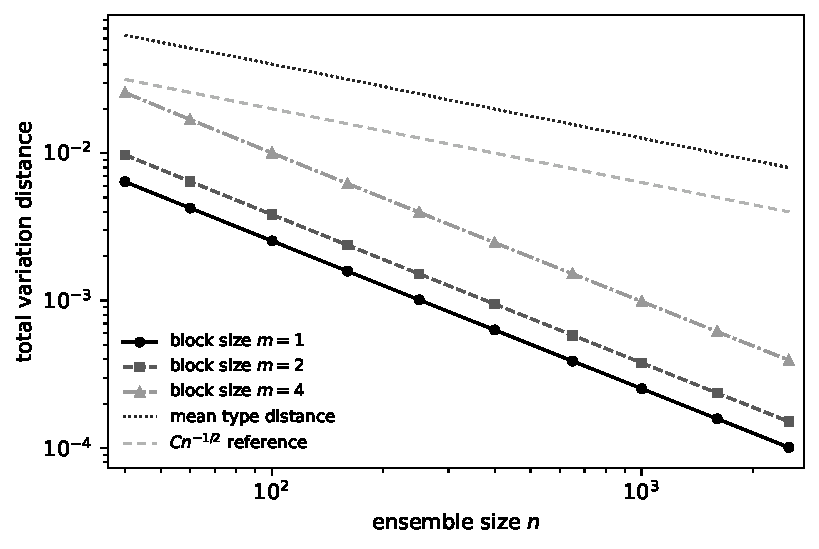
\includegraphics[width=0.52\textwidth]{fig_direct_block_collapse}
 \caption{Exact conditional block collapse on a three-cell chart.
 Solid and broken curves give
 $\TV\{\mu_{n,m},(p^*)^{\otimes m}\}$ for fixed
 $m\in\{1,2,4\}$; the dotted curve is the conditional mean
 $\E\{\TV(\widehat p,p^*)\}$, and the gray broken line is an
 $n^{-1/2}$ reference. The type spread has the Gaussian scale from
 Theorem~\ref{thm:gdf}, while every fixed-block distance vanishes as
 asserted by Theorem~\ref{thm:collapse}.}
 \label{fig:direct-collapse}
 \end{figure}

The mean type distance follows the expected $n^{-1/2}$ scale. The block
distances decrease faster in this example because mixing cancels the
first-order centered type fluctuation; Theorem~\ref{thm:collapse} supplies
an upper bound rather than an exact asymptotic rate. Enumeration details
are in the Supplementary Material, \S\,S9.

\subsubsection{Parametric design}

The second illustration is designed to display the parametric geometry
rather than to rank the estimators. We adapt the mean-and-variance
constraint problem
of Schennach (2007), Section~4, retaining its moment functions but
using a more pronounced misspecified regime. For $X_1,\ldots,X_n$ from a
location--scale normal model, the moment functions
$g(x,\theta)=\{x-\theta,\,(x-\theta)^2-1\}$ give a constraint
$\E\{g(X,\theta_0)\}=0$ that identifies the mean $\theta_0$ while pinning
the variance to one. Given $\E X=\theta$, the second condition reads $\E X^2=1+\theta^2$, so the constraint set is that of the fixed moment map $h(x)=(x,x^2)$ with target $\alpha(\theta)=(\theta,1+\theta^2)$: the cell-moment matrix $A_r$ does not move with $\theta$, as~\eqref{eq:icl-est} and Proposition~\ref{thm:gmm} require. We consider two regimes: Model~C, with
$X_i\sim\N(0,1)$, correctly specified; and Model~M, with $X_i\sim\N(0,4)$,
in which the variance constraint is misspecified (a fourfold variance
ratio). The baseline $Q$ is $\N(0,1)$ and we use a quantile partition of
size $k_r=20$, on which $q_r$ is uniform. Because the extreme cells are
unbounded, Assumption~\ref{ass:refine} does not apply to this fixed chart.
We therefore treat $k_r=20$ as a fixed-chart calculation and compute the
finite cell moments $h_r(j)$ in closed form from the truncated-normal
formulae.

\begin{samepage}
The four laws used below have distinct roles:
\begin{center}
\small
\begin{tabular}{@{}ll@{}}
$q_r$ & fixed baseline cell law; also $p_{\theta_0,r}^*$ in this design,\\
$q_{M,r}$ & cell law of the misspecified data-generating distribution,\\
$p_{M,r}^*$ & projection of $q_{M,r}$, used for change-of-measure geometry,\\
$p_{\theta,r}^*$ & parameter-indexed projection used for inference.
\end{tabular}
\end{center}
\end{samepage}

The two tilted procedures enforce both moments but differ in support: the
ETEL (exponentially tilted empirical likelihood) maximizer of the BETEL (Bayesian ETEL) profile (Schennach, 2005), labeled
$\hat\theta_{\text{\textsc{betel}}}$, tilts the realized sample, whereas
$\hat\theta_{\text{\textsc{icl}}}$ tilts the fixed partition cells. The
separate benchmark $\hat\theta_{\text{\textsc{gmm}}}=\bar X$ uses only the
correctly specified location moment and leaves the variance restriction
unused. This variance-agnostic reference is specific to the present section,
not to Schennach (2007) (Supplementary Material, \S\,S9).

\subsubsection{Geometric structure}\label{sec:sim-geometry}

Figure~\ref{fig:geometry-projection} shows the Model-M cell law
$q_{M,r}$ and its information projection $p_{M,r}^*$ onto the constraint
set. This change-of-measure projection is distinct from the parametric
pseudo-true law $p_{\theta_0,r}^*$ of \S\,\ref{sec:moment-misspec}; here the
baseline cell law already satisfies the constraints, so
$p_{\theta_0,r}^*=p_r^*=q_r$. The variance restriction moves mass from
the extreme cells toward the center, with
$\D{p_{M,r}^*}{q_{M,r}}\approx0{.}269$.

Figure~\ref{fig:curv-collapse} gives two complementary diagnostics.
The condition number of the change-of-measure curvature is one under
Model~C and reaches $1{.}379$ at $k_r=80$ under Model~M. The mean
empirical discrepancy $\TV(\widehat p_n,p_r^*)$ decays at the rate
$O\{(k_r/n)^{1/2}\}$ under Model~C but approaches
$\TV(q_{M,r},p_r^*)\approx0{.}322$ under Model~M. This diagnostic
concerns misspecification and is distinct from the conditional
block-predictive law of Theorem~\ref{thm:collapse}; likewise, $p_{M,r}^*$
is a separate object, with $\TV(q_{M,r},p_{M,r}^*)\approx0{.}326$.

\begin{figure}[H]
 \centering
 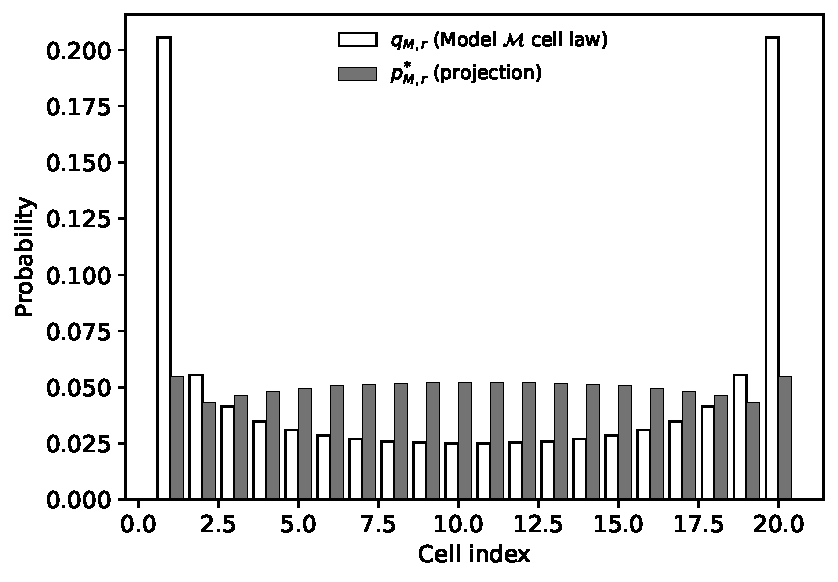
\includegraphics[width=0.55\textwidth]{fig_geometry_projection}
 \caption{Information projection under Model~M ($k_r=20$,
 $\sigma=2$): cell law
 $q_{M,r}$ of the $\N(0,4)$ measure and its information projection
 $p_{M,r}^*$, which redistributes the extreme-cell mass toward the
 center to satisfy the variance constraint ($\D{p_{M,r}^*}{q_{M,r}}\approx 0{.}269$).}
 \label{fig:geometry-projection}
 \end{figure}

\begin{figure}[H]
 \centering
 \begin{minipage}[t]{0.45\textwidth}
 \centering
 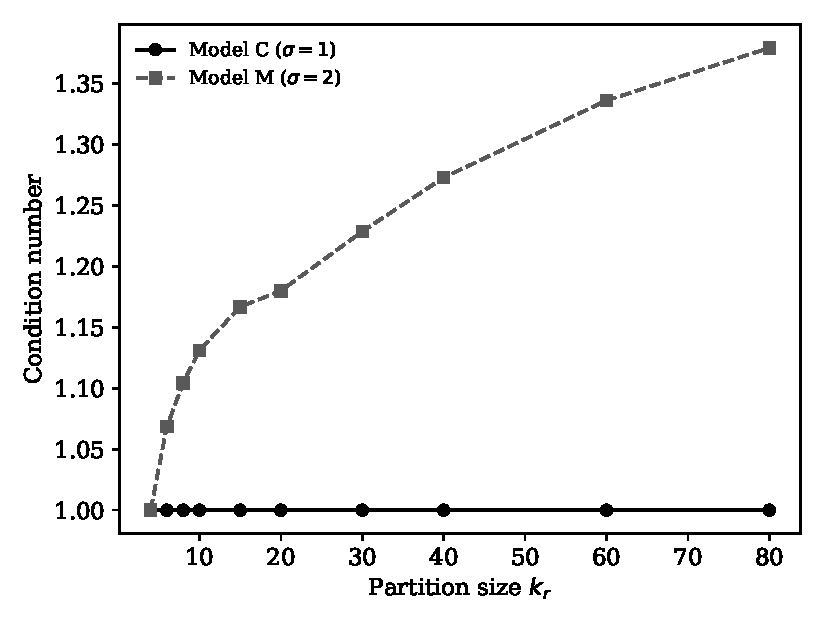
\includegraphics[width=\linewidth]{fig_curvature_refinement}
 \end{minipage}\hfill
 \begin{minipage}[t]{0.45\textwidth}
 \centering
 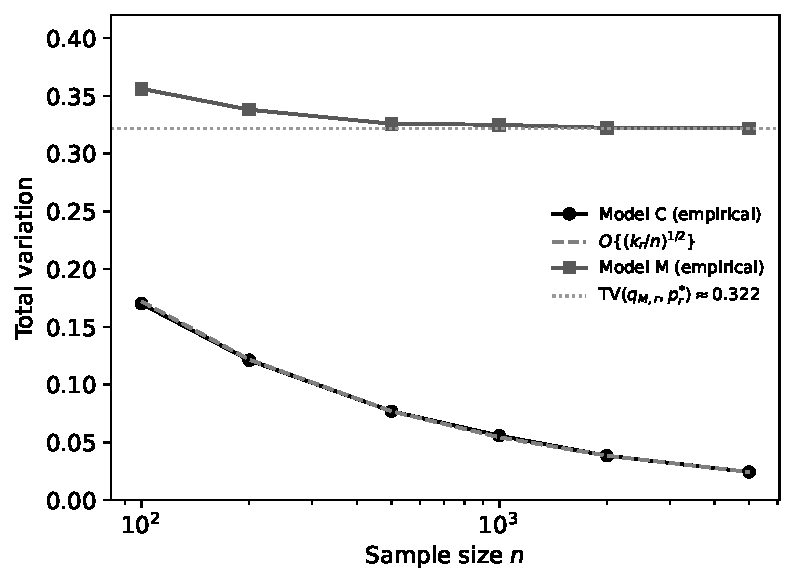
\includegraphics[width=\linewidth]{fig_predictive_collapse}
 \end{minipage}
 \caption{Left: condition number $\kappa(H_{M,r}^*)$ of the Model-M
 change-of-measure projection $q_{M,r}\to p_{M,r}^*$ ($H_{M,r}^*$ its
 reduced Hessian, distinct from the baseline $H_r^*$), isotropic under
 Model~C and growing to $\kappa\approx 1{.}379$ at $k_r=80$ under
 Model~M. Right: empirical
 cell discrepancy $\TV(\widehat p_n,p_r^*)$ versus $n$ ($k_r=20$,
 $500$ replications); under Model~C it tracks $O\{(k_r/n)^{1/2}\}$,
 under Model~M it converges to the floor
 $\TV(q_{M,r},p_r^*)\approx 0{.}322$.}
 \label{fig:curv-collapse}
 \end{figure}

\subsubsection{Comparison of estimation procedures}\label{sec:comparison-est}

Table~\ref{tab:sim} reports the Monte Carlo standard deviation and
bias of each estimator over $2000$ replications at sample sizes
$n\in\{1000,5000\}$. Under Model~C all three procedures behave
similarly, as expected when the moment conditions are correctly
specified. Under Model~M a dispersion difference emerges:
$\hat\theta_{\text{\textsc{betel}}}$ becomes more dispersed, while
$\hat\theta_{\text{\textsc{icl}}}$ remains close to $\hat\theta_{\text{\textsc{gmm}}}$
(Supplementary Material, Fig.~S1). Biases are
negligible in both regimes.

\begin{table}[htbp]
 \centering
 \caption{Monte Carlo standard deviation ($\times 10^2$) and bias
 ($\times 10^4$) for estimation of $\theta_0=0$.
 Model~C: $X_i\sim\N(0,1)$; Model~M: $X_i\sim\N(0,4)$.
 Each entry is based on $2000$ replications; Monte Carlo standard
 errors of the bias entries range from $3$ to $23$ in the same
 units. The final column is the mean total-variation discrepancy
 $\TV(\widehat p_n,p_r^*)$ of \S\,\ref{sec:sim-geometry}.
 The entries are those of Table~1 of the source paper (arXiv:2510.20742); computational details are
 in its Supplementary Material, \S\,S9.}\label{tab:sim}
 \begin{tabular}{llrrrrrrr}
 \toprule
 && \multicolumn{3}{c}{Standard deviation} &
 \multicolumn{3}{c}{Bias} & Mean \\
 \cmidrule(lr){3-5}\cmidrule(lr){6-8}
 Model & $n$ & \textsc{gmm} & \textsc{betel} & \textsc{icl} &
 \textsc{gmm} & \textsc{betel} & \textsc{icl} & TV \\
 \midrule
 C & 1000 & 3.157 & 3.170 & 3.122 & $-5.7$ & $-6.1$ & $-5.8$ & 0.055 \\
 C & 5000 & 1.406 & 1.407 & 1.402 & $2.0$ & $2.0$ & $2.4$ & 0.025 \\
 M & 1000 & 6.409 & 10.329 & 6.231 & $-7.4$ & $-19.8$ & $-6.3$ & 0.324 \\
 M & 5000 & 2.792 & 4.539 & 2.711 & $3.5$ & $2.6$ & $5.6$ & 0.322 \\
 \bottomrule
 \end{tabular}
\end{table}

Under Model~M, the last column of Table~\ref{tab:sim} approaches the floor
$0{.}322$. This comparison illustrates the distinction between
specification and misspecification; the relative performance of the
estimators remains specific to this design.



%% ====================================================================
\subsection{Discussion}\label{sec:discussion}
%% ====================================================================

The central gain from conditioning is a probabilistic interpretation of the
information projection. The exact type mixture separates two mechanisms:
the conditional empirical type concentrates near $p_r^*$, and sampling a
fixed block without replacement becomes sampling from its cell
probabilities. Lattice regularity sharpens the first mechanism to a
Gaussian statement; the shrinking-window argument retains the predictive
conclusion when that arithmetic structure is absent.

The reference law remains indispensable. Moment restrictions alone do not
identify a predictive distribution, and changing $Q$ changes both the
projection and its curvature. Refinement controls the chart approximation
for a fixed reference construction; it does not remove this modeling
choice. Parameterization is a second operation: differentiating the
projected family produces parameter information and the local
generalized-method-of-moments criterion. This explains why tangent
curvature, parameter information and misspecification risk curvature play
different roles.

The main limitation is that the concentration results are proved on a fixed
chart, with constants that need not remain controlled under refinement. A
uniform theory in which chart dimension and block size grow together would
require stable normalization of the curvature spectrum and joint control of
refinement, localization and finite-population error. Such control would
replace the present diagonal existence argument by an explicit joint
regime. Partial exchangeability and sequential prediction provide natural
further settings for the same probabilistic construction.


\paragraph{Summary.}
Predictive geometry views moment conditioning as $I$-projection onto an affine family of constraints, and the predictive distribution as a point moving along the resulting exponential family. For independent draws from a fixed baseline on a finite chart, the law of a block given the moment event is an exact mixture over empirical types. Under lattice regularity the mixing law has a Gaussian limit with precision the reduced Hessian $H_r^*$ (Theorem~\ref{thm:gdf}), and the block collapses to independent draws from the projection, $(p_r^*)^{\otimes m}$, with a total variation bound whose first term is the Gaussian tangential spread (Theorem~\ref{thm:collapse}). A shrinking window keeps the collapse, with a coarser bound, when lattice regularity fails (Theorem~\ref{thm:window}), and a diagonal sequence of charts lifts it to the original sample space (Corollary~\ref{cor:joint}). Parameterizing the projected family gives the induced conditional likelihood, whose local quadratic expansion carries the optimal covariance weighting of the generalized method of moments and whose parameter information $\Info_{\theta,r}=\dot\alpha(\theta)^\top\Omega_{\theta,r}^{-1}\dot\alpha(\theta)$ is distinct from the tangent curvature $H_r^*$.

\subsection*{Problems}
\begin{enumerate}[leftmargin=2.2em,itemsep=2pt]
\item Show that conditioning on a moment $\E[f]=a$ is $I$-projection onto an affine constraint set and yields an exponential tilt.
\item Verify the dual-flatness of the exponential family in the natural and mean parameterizations.
\item State and prove the information-geometric Pythagorean theorem for the projection.
\item Compute the Fisher--Rao metric for a one-parameter exponential family and relate it to the second derivative of the log-partition function.
\item Interpret moment conditioning as a predictive update and connect it to the tilted de Finetti theorem.
\item In the three-cell example of \S\,\ref{sec:sim-direct}, with $\psi(\lambda)=\log\sum_jq_je^{\lambda h_j}$, solve $\psi'(\lambda^*)=0$ to show that $\lambda^*=\tfrac12\log(2/3)$ and $p^*=(0{.}24745,0{.}50510,0{.}24745)$. Show that the tangent space~\eqref{eq:tangent} is spanned by $(1,-2,1)^\top$ and that the reduced Hessian~\eqref{eq:hessian} is $H^*=\tfrac16(2/p_1^*+4/p_2^*)\approx2{.}667$.
\item In the same example, the weight~\eqref{eq:typeweight} of the type with counts $(t,n-2t,t)$ is proportional to $\binom{n}{t,\,t,\,n-2t}(q_1q_3)^tq_2^{\,n-2t}$. With $V=(1,-2,1)^\top/\sqrt6$, write $t=np_1^*+u\sqrt{n/6}$ and use Lemmas~\ref{lem:tail} and~\ref{lem:gaussian}, the tail bound and the Gaussian form of the type weights behind Theorem~\ref{thm:gdf}, to show that $(t-np_1^*)/\sqrt n$ is asymptotically normal with variance $1/(2/p_1^*+4/p_2^*)\approx0{.}0625$.
\item Suppose $\lambda_{\min}(H_r^*)\ge c\,k_r$ for some $c>0$, as on a balanced chart. Show that $\tr\{(H_r^*)^{-1}\}\le s_r/(ck_r)\le1/c$, so that the first term of~\eqref{eq:collapse} is at most $m\{k_r/(cn)\}^{1/2}$, and find the block sizes $m$ for which the collision term $m(m-1)/n$ exceeds this bound.
\item Prove the identity $\Info_{\theta,r}=\dot\alpha(\theta)^\top\Omega_{\theta,r}^{-1}\dot\alpha(\theta)$ of Proposition~\ref{thm:gmm}. Differentiate the Gibbs form~\eqref{eq:discrete-gibbs}, with $\lambda_{\theta,r}^*$ in place of $\lambda_r^*$, to show that $J_{\theta,r}=\Sigma_{\theta,r}A_r^\top\,\partial\lambda_{\theta,r}^*/\partial\theta^\top$; differentiate $A_rp_{\theta,r}^*=\alpha(\theta)$ to solve for $\partial\lambda_{\theta,r}^*/\partial\theta^\top$; and use $\Sigma_{\theta,r}\diag(1/p_{\theta,r}^*)\Sigma_{\theta,r}=\Sigma_{\theta,r}$ in~\eqref{eq:param-info}.
\end{enumerate}

\src{Bayesian Prediction under Moment Conditioning (2510.20742), full text; companion to De Finetti + Sanov = Bayes (2509.13283). Extended proofs in the supplementary material of the source paper.}

%==========================================================================================

\shorthead{Maximum Entropy Algorithms}
\section{Maximum Entropy Algorithms}\label{ch:maxent}

\noindent\textbf{Thesis.} Raking a table, tilting an empirical measure, allocating attention, and
quantizing a source are one operation, I-projection, computed by one master routine, alternating
minimization, whose four faces are iterative proportional fitting, Dykstra--Bregman,
Blahut--Arimoto, and majorization. The Gibbs rule is a proximal operator\index{proximal operator}; the mutual-information
Hessian in a published identification diagnostic is not positive semidefinite, and its Gauss--Newton part, the envelope curvature,
repairs it.

Sections~\ref{ch:types} and~\ref{ch:sanov} established the objects this section computes. Sanov's
theorem (Theorem~\ref{thm:sanov}) makes $\D{\cdot}{P}$ a rate function and the I-projection the
cheapest constraint-satisfier; the conditional limit theorem (Theorem~\ref{thm:vcc}) shows that
conditioning an i.i.d.\ sample on an empirical constraint produces the exponential tilt, which
is why the tilt is a theorem rather than a modeling convenience. What remains is the question those
sections did not ask: given the projection, how does one \emph{compute} it? The answer is short,
because it is organized by two questions.

\subsection{Five literatures, one construction}
\label{sec:me-intro}

Demographers rake a contingency table to known margins. Econometricians tilt the empirical measure
to satisfy a moment condition. Macroeconomists give an agent finite attention and ask what she
chooses to look at. Choice modelers derive multinomial logit. Information theorists compute a
rate--distortion function. Each begins from a baseline distribution, imposes constraints, and takes
the closest distribution satisfying them, with closeness measured in relative entropy. Each ends at
an exponential tilt of the baseline. The notation differs; the mathematics does not.

\begin{center}\footnotesize
\begin{tabular}{@{}lll@{}}
\toprule
 & \textbf{Equality constraints} & \textbf{Inequality constraints} \\
\midrule
\textbf{Fixed baseline}
 & Iterative proportional fitting (\S\ref{sec:me-ipf})
 & Dykstra--Bregman (\S\ref{sec:me-dykstra}) \\
 & \emph{Stern--Cover lottery} & \emph{moment inequalities} \\
\addlinespace
\textbf{Self-consistent baseline}
 & Blahut--Arimoto (\S\ref{sec:me-blahut})
 & open (\S\ref{sec:me-discussion}) \\
 & \emph{Sims; rate--distortion} & \\
\bottomrule
\end{tabular}
\end{center}

``Fixed'' means the baseline $P$ is given exogenously, as in Section~\ref{ch:sanov}.
``Self-consistent'' means the baseline is the marginal induced by the rule itself, so that the fixed
point must be solved for. That single distinction separates raking from rate--distortion, and it is
why Blahut--Arimoto exists as a separate algorithm rather than as a footnote to iterative scaling. A
parametric restriction on the rule cuts across the table and forces majorization
(\S\ref{sec:me-mm}); all four faces are instances of one alternating minimization
(\S\ref{sec:me-alternating}).

Underneath sits one conjugacy. The mixture representation of a model, which integrates out a latent
scale, and its envelope representation, which minimizes out a latent scale, are Fenchel duals
related by Laplace's method (Polson and Scott, 2016). P\'olya--Gamma augmentation and the Bouchard
bound are two faces of a single object. Integration and minimization are the same operation at
different temperatures, and that one line explains why Sanov's rate function is the conjugate of a
cumulant generating function, why the log-partition is an envelope, and why the Gibbs rule
concentrates on the utility maximizer as the price of information falls (\S\ref{sec:me-mixenv}).

\paragraph{Terminology.}
We reserve \emph{maximum entropy} for a uniform baseline, where minimizing $\D{p}{p_0}$
maximizes $H(p)$. Otherwise the object is minimum relative entropy, minimum discrimination
information (Kullback, 1959), or I-projection (Csisz\'ar, 1975). The distinction earns its keep:
Stern and Cover have a uniform baseline over $\binom{49}{6}$ combinations and are entitled to the
term; a predictive rule tilted from its own marginal is not. The title and the remarks on limitations below follow common usage and apply the name to the whole family of methods.

\subsection{The I-projection restated for computation}
\label{sec:me-iproj}

Section~\ref{ch:sanov} gave the I-projection and the Pythagorean inequality. Computation needs two
further facts: the duality that makes the log-partition an envelope, which is what
\S\ref{sec:me-prox} builds on, and the characterization of the projection onto a set that is convex
but not affine, which is what separates \S\ref{sec:me-ipf} from \S\ref{sec:me-dykstra}. We restate
the projection in the notation used for the rest of the section, writing $p_0$ for the baseline.

\begin{theorem}[Tilt, Pythagoras, duality]
\label{thm:me-tilt}
Let $p_0>0$ on $\X$ and $\mathcal{C}=\{p:\E_p[T]=t\}$ for $T:\X\to\R^d$, with $t$ in the relative interior of the convex hull of
$T(\X)$. Then:
\begin{enumerate}
 \item[(i)] \textup{(Tilt.)} The solution of $\min_{p\in\mathcal{C}}\D{p}{p_0}$ is the exponential
 family member
 \begin{equation}
 \label{eq:me-expfam}
 p^\star(x)=\frac{p_0(x)e^{\theta^\top T(x)}}{Z(\theta)},
 \qquad Z(\theta)=\sum_x p_0(x)e^{\theta^\top T(x)},
 \end{equation}
 with $\theta$ a solution of $\nabla_\theta \log Z(\theta)=t$, unique when $T(\X)$ lies in no hyperplane; $p^\star$ is unique in any case.
 \item[(ii)] \textup{(Pythagoras.)} For every $p\in\mathcal{C}$,
 $\D{p}{p_0}=\D{p}{p^\star}+\D{p^\star}{p_0}$.
 \item[(iii)] \textup{(Duality.)} $\D{p^\star}{p_0}=\sup_\theta\{\theta^\top t-\log Z(\theta)\}$,
 and $\theta\mapsto\log Z(\theta)$ and $t\mapsto\D{p^\star}{p_0}$ form a Legendre\index{Legendre transform} pair.
\end{enumerate}
\end{theorem}

Parts (i) and (ii) are Section~\ref{ch:sanov} in the present notation; on an affine set the
Csisz\'ar inequality holds with equality, which is the form used below. Part (iii) is the new
content: it identifies $\log Z$ as the convex conjugate of relative entropy, and
\S\ref{sec:me-prox} shows that this makes the Gibbs rule a proximal operator. A proof is given
at the end of this section.

Part (ii) is the engine of the section: it converts a minimization into an identity, and it is what
makes cyclic projection work in \S\ref{sec:me-ipf} and fail in \S\ref{sec:me-dykstra}.

\subsubsection{General constraint sets}

Theorem~\ref{thm:me-tilt} assumed a moment set. For the polyhedral sets of \S\ref{sec:me-dykstra}
we need the general characterization, which is a variational inequality rather than a first-order
equation.

\begin{proposition}[Csisz\'ar, 1975]
\label{prop:me-varineq}
$p^\star\in\mathcal{C}$ is the I-projection of $p_0$ onto a closed convex $\mathcal{C}$ if and only
if
\begin{equation}
\label{eq:me-varineq}
 \sum_x \big(p(x)-p^\star(x)\big)\log\frac{p^\star(x)}{p_0(x)} \;\ge\; 0
 \qquad \text{for every } p\in\mathcal{C},
\end{equation}
in which case Pythagoras holds as an inequality, $\D{p}{p_0}\ge\D{p}{p^\star}+\D{p^\star}{p_0}$ for
all $p\in\mathcal{C}$.
\end{proposition}

Read \eqref{eq:me-varineq} as the statement that the log-likelihood ratio $\log(p^\star/p_0)$ is a
supporting functional for $\mathcal{C}$ at $p^\star$: it cannot decrease as one moves into the set.
When $\mathcal{C}$ is affine one may move in either direction along it, \eqref{eq:me-varineq} holds
with equality, and Pythagoras becomes the identity of Theorem~\ref{thm:me-tilt}(ii). When
$\mathcal{C}$ has a boundary one may only move inward, the inequality can be strict off the active face,
and the identity is lost. That is the entire difference between \S\ref{sec:me-ipf} and
\S\ref{sec:me-dykstra}, stated once. It is also the reason the divergence-gap bound \eqref{eq:gap}
of Section~\ref{ch:sanov} is stated as an inequality: the same boundary effect.

\subsubsection{The econometric cousin}

The finite-sample tilt is already standard in econometrics, and it is the fixed-baseline, equality
cell evaluated at $\Phat_n$. Given moments $\E[g(Z,\beta)]=0$, exponentially tilted empirical
likelihood (Kitamura and Stutzer, 1997; Imbens, Spady and Johnson, 1998; Schennach, 2007) assigns
\[
 w_i(\beta)=\frac{\exp\{\gamma(\beta)^\top g(Z_i,\beta)\}}
 {\sum_{j\le n}\exp\{\gamma(\beta)^\top g(Z_j,\beta)\}},
 \qquad
 \gamma(\beta)=\arg\min_\gamma \frac1n\sum_{i\le n} e^{\gamma^\top g(Z_i,\beta)} .
\]
These weights are the I-projection of $\Phat_n$ onto the moment set, and $\gamma$ is the multiplier
$\theta$ of \eqref{eq:me-expfam}. Empirical likelihood proper (Owen, 2001) reverses the divergence
and so sits elsewhere in the Cressie--Read family, which is why the two agree to first order and
differ beyond it (Newey and Smith, 2004). Their projection and the book's differ only in the baseline: theirs projects the
empirical measure onto a moment set, ours projects a predictive rule away from its own marginal.

%---------------------------------------------------------------------
\subsection{Alternating Minimization: the Master Algorithm}
\label{sec:me-alternating}

Every algorithm in this section is one algorithm. State it once.

Let $\mathcal{C}_1,\mathcal{C}_2$ be closed convex sets and let $D$ be a
jointly convex divergence between measures, with values in $(-\infty,\infty]$.
Consider
\[
 \min_{u\in\mathcal{C}_1,\ v\in\mathcal{C}_2} D(u,v),
 \qquad
 u^{t+1}=\arg\min_{u\in\mathcal{C}_1} D(u,v^t),
 \qquad
 v^{t+1}=\arg\min_{v\in\mathcal{C}_2} D(u^{t+1},v).
\]

\begin{definition}[Five-point property]
$D$ has the \emph{five-point property} for $(\mathcal{C}_1,\mathcal{C}_2)$ if for
every $u\in\mathcal{C}_1$, $v\in\mathcal{C}_2$ and every $t\ge1$,
\begin{equation}
\label{eq:me-fivepoint}
 D(u,v)+D(u,v^{t-1}) \;\ge\; D(u,v^t)+D(u^t,v^{t-1}).
\end{equation}
\end{definition}

The name counts the arguments: $u,v,v^{t-1},v^t,u^t$. The content is that the
divergence, though asymmetric and lacking a triangle inequality, still behaves
enough like a squared Euclidean distance for the alternating argument to close.
Monotonicity needs no five-point property, since each half-step minimizes; summing \eqref{eq:me-fivepoint} over $t$
telescopes the terms $D(u,v^t)$, and the infimum over pairs
$(u,v)\in\mathcal{C}_1\times\mathcal{C}_2$, taken after summing, gives the
convergence claim.

\begin{theorem}[Csisz\'ar and Tusn\'ady, 1984]
\label{thm:me-csiszar-tusnady}
If $D$ satisfies the five-point property \eqref{eq:me-fivepoint} and $D(u,v^0)<\infty$ for every $u\in\mathcal{C}_1$, the alternating
iterates obey $D(u^{t+1},v^{t+1})\le D(u^t,v^t)$ and converge to
$\inf_{\mathcal{C}_1\times\mathcal{C}_2} D$. Relative entropy, $D(u,v)=\D{u}{v}$, satisfies it when, on a finite alphabet, $\mathcal{C}_1$ is a closed convex set of probability measures and $\mathcal{C}_2$ a closed convex set of finite measures (against which $D$ can be negative), and
the minimization over $u$ is then an exact $I$-projection and that over $v$ a reverse $I$-projection.
\end{theorem}

Three features of Theorem~\ref{thm:me-csiszar-tusnady} deserve emphasis, because
they are what the alternating schemes buy and what gradient methods do not. There
is no step size. There is no smoothness constant. And monotonicity is
unconditional, not asymptotic.

\subsubsection{The geometry, and why it works}

The picture is worth carrying. Two convex sets, $\mathcal{C}_1$ and
$\mathcal{C}_2$, sit inside a space of measures. The alternating scheme starts
somewhere in $\mathcal{C}_2$, projects to the nearest point of $\mathcal{C}_1$,
projects that back to the nearest point of $\mathcal{C}_2$, and repeats. If the
sets intersect, the iterates converge to the intersection. If they do not, the
iterates converge to the pair of points realizing the minimum distance between
them. Either way, distance decreases at every half-step, because a projection
cannot move you further from the set you projected onto.

That last sentence is the whole proof of monotonicity, and it is also where the subtlety hides.
``Distance'' here is a divergence, not a metric: it is asymmetric, it fails the
triangle inequality, and decrease at every half-step does not by itself carry the
iterates to the infimum. The five-point property
is the condition that repairs this. Relative entropy has it; a general
Bregman divergence need not.

Why insist on exact minimization at each half-step rather than a gradient step?
Because exactness is what buys the guarantees. A gradient step requires a step
size, which requires a smoothness constant, which requires an estimate the user
must supply and may get wrong. An exact $I$-projection requires nothing: it is a
closed-form tilt by Theorem~\ref{thm:me-tilt}, and the monotonicity is
unconditional. When practitioners reach for mirror descent to solve a problem
that Blahut--Arimoto solves exactly, they are trading a guarantee for a tuning
parameter, and receiving nothing in exchange.

\subsubsection{EM is in this table}

The claim that EM belongs here is worth substantiating, since it is the instance
most readers will already know and it makes the pattern visible.

Let $y$ be observed, $z$ latent, and $p_\theta(y,z)$ a model. Take
$\mathcal{C}_1$ to be the set of distributions $q(z)$ over the latent variable,
$\mathcal{C}_2$ the parameter space, and
$D(q,\theta)=D(q(z)\|p_\theta(z\mid y))-\log p_\theta(y)$, which is the negative
evidence lower bound\index{evidence lower bound}. Minimizing over $q$ with $\theta$ fixed gives
$q^{t+1}(z)=p_{\theta^t}(z\mid y)$: that is the E step, and it is an exact
$I$-projection onto $\mathcal{C}_1$. Minimizing over $\theta$ with $q$ fixed gives
$\theta^{t+1}=\arg\max_\theta \E_{q^{t+1}}[\log p_\theta(y,z)]$: that is
the M step. The negative evidence lower bound pairs a law with a parameter, so it is not a divergence in the sense of Theorem~\ref{thm:me-csiszar-tusnady}, which therefore does not apply as stated. The two exact minimizations alone give
\[
 -\log p_{\theta^{t+1}}(y)\le D(q^{t+1},\theta^{t+1})\le D(q^{t+1},\theta^t)=-\log p_{\theta^t}(y),
\]
the first inequality because the relative entropy term is nonnegative. That is monotone increase
of the likelihood, which is the classical EM guarantee. Convergence to the
infimum does not transfer, and EM can stop at a local maximum.

The same reading explains the family resemblances that are otherwise puzzling. EM
has no step size, and neither does Blahut--Arimoto, and neither does IPF, for the
same reason: all three replace a gradient step by an exact projection. All three
are monotone unconditionally. All three can be slow, because exactness in one
coordinate says nothing about progress in the other, and all three are therefore
vulnerable to the same pathology, namely a long narrow valley between the two
sets. Recognizing the common structure means one does not have to learn these
facts three times.

\begin{center}\footnotesize
\begin{tabular}{@{}llll@{}}
\toprule
\textbf{Algorithm} & $\mathcal{C}_1$ & $\mathcal{C}_2$ & \textbf{Section} \\
\midrule
IPF / generalized iterative scaling & constraint set $k$ & constraint set $k+1$ & \S\ref{sec:me-ipf} \\
Dykstra--Bregman & constraint set $k$, corrected & $\cdots$ & \S\ref{sec:me-dykstra} \\
Blahut--Arimoto & channels $q(y\mid x)$ & marginals $m(y)$ & \S\ref{sec:me-blahut} \\
Majorize--minorize & surrogate at $\theta^t$ & parameter space & \S\ref{sec:me-mm} \\
EM & latent laws $q(z)$ & parameters $\theta$ & \S\ref{sec:me-alternating} \\
\bottomrule
\end{tabular}
\end{center}

%---------------------------------------------------------------------
\subsection{Fixed Baseline, Equality Constraints: Iterative Scaling}
\label{sec:me-ipf}

The classical cell. The baseline is given, the constraints are marginal or moment
equalities, and the constraint sets are affine.

\subsubsection{Iterative proportional fitting}

For a two-way table with seed $p_0(i,j)$ and prescribed margins $r_i,c_j$, IPF
alternates
\[
 p^{(2t+1)}(i,j)=p^{(2t)}(i,j)\cdot\frac{r_i}{p^{(2t)}(i,\cdot)},
 \qquad
 p^{(2t+2)}(i,j)=p^{(2t+1)}(i,j)\cdot\frac{c_j}{p^{(2t+1)}(\cdot,j)} .
\]
Each half-step is an exact $I$-projection onto one affine set, and
Theorem~\ref{thm:me-cyclic} below identifies the limit as the $I$-projection of $p_0$ onto the set of tables with both margins. Deming and Stephan (1940) proposed
it; Sinkhorn (1964) proved existence and uniqueness of the scaling;
Fienberg (1970) gave a geometric proof of its convergence for two-way tables. The following is the result on
which the entire cell rests.

\begin{theorem}[Csisz\'ar, 1975]
\label{thm:me-cyclic}
If $\mathcal{C}_1,\dots,\mathcal{C}_m$ are affine with
$\bigcap_k \mathcal{C}_k\neq\emptyset$, cyclic $I$-projection converges to the
$I$-projection of $p_0$ onto $\bigcap_k \mathcal{C}_k$.
\end{theorem}

Affineness is not decorative. By Theorem~\ref{thm:me-tilt}(ii), Pythagoras holds
with equality at each step because on an affine set one may move either way
along the set, so that \eqref{eq:me-varineq} holds with equality. Drop affineness, the equality becomes an inequality, the
bookkeeping fails, and the limit is the wrong point. That is
\S\ref{sec:me-dykstra}, and it is the most common error in applied use of these
methods.

\subsubsection{Generalized iterative scaling}

Darroch and Ratcliff (1972) extend IPF to nonnegative features $T_j(x)\ge0$ with
$\sum_j T_j(x)=m$ constant. The dual ascent step is multiplicative: with
$w_j=e^{\theta_j}$,
\begin{equation}
\label{eq:me-gis}
 w_j^{(k+1)} = w_j^{(k)}\left(\frac{t_j}{\E_{p^{(k)}}[T_j]}\right)^{1/m}.
\end{equation}
Improved iterative scaling (Della Pietra, Della Pietra and Lafferty, 1997) removes the constant-sum
condition. Sinkhorn scaling is the same algorithm as entropic optimal transport\index{optimal transport}
(Cuturi, 2013; Peyr\'e and Cuturi, 2019); what distinguishes us from that literature is the baseline,
since optimal transport fixes both margins whereas \S\ref{sec:me-blahut} fixes one
and solves for the other.

\subsubsection{Stern and Cover (1989): the lottery}
\label{sec:me-lottery}

The canonical statistical instance, worth working in full because its baseline is
uniform.

\paragraph{An impossible problem.}
In Canada's Lotto 6/49, bettors choose $m=6$ numbers from $M=49$. The object of
interest is the distribution $p$ over the $\binom{49}{6}=13{,}983{,}816$
combinations actually purchased, because a parimutuel jackpot is shared and the
value of a ticket depends on how many others hold it. The lottery publishes only
the marginals: the proportion $\pi_i$ of tickets containing number $i$. That is 48
free constraints on a simplex of dimension $1.4\times10^7$. No nonparametric
estimate exists.

\begin{figure}[htbp]
\centering
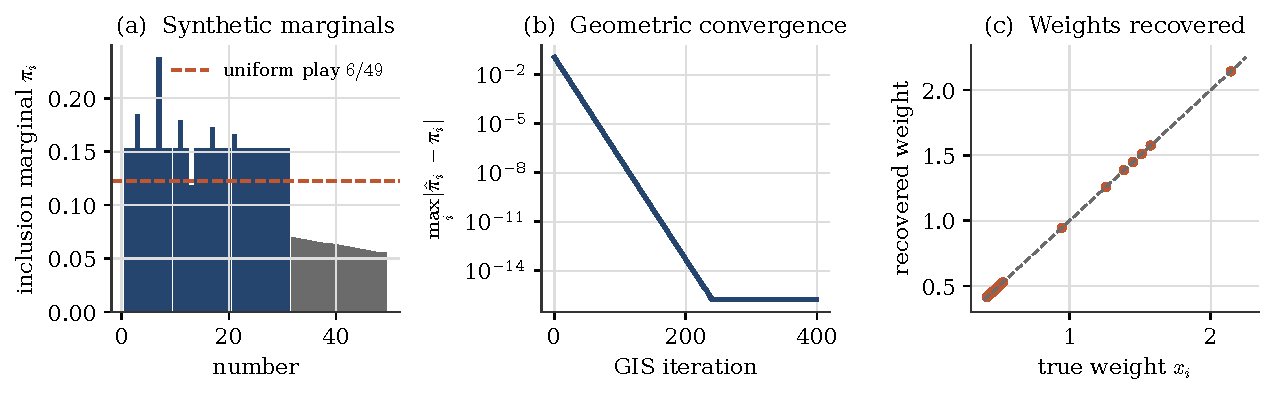
\includegraphics[width=\textwidth]{fig_lottery_gis}
\caption{Stern and Cover reconstructed. (a) The inclusion marginals are the only
input to the fit, and here they are synthetic: birthday numbers (dark) are set over played and high numbers under played. (b) Generalized
iterative scaling drives the fitted marginals to those of (a) at a geometric rate.
(c) Recovered weights match the generating weights to $10^{-15}$, pinning down a distribution over
$1.4\times10^7$ combinations from 48 free constraints, entirely through $e_5$ and $e_6$.}
\label{fig:me-lottery}
\end{figure}

\paragraph{The resolution.}
Take the baseline uniform over combinations and apply
Theorem~\ref{thm:vcc}: if bettors' choices are i.i.d.\ draws from the baseline and we
condition on the observed marginals, the limiting law of a single ticket is the
constrained maximum entropy distribution. This is a substantive behavioral
assumption, and Stern and Cover say so. It converts an impossible problem into a
48-parameter one: the tilt has 49 multipliers, but adding a common constant to all of them leaves it unchanged.

\paragraph{Product form.}
The sufficient statistic is the incidence vector
$T(c)=(\mathbf{1}\{i\in c\})_{i\le49}$, so \eqref{eq:me-expfam} gives
\begin{equation}
\label{eq:me-condbern}
 p^\star(c) = \frac{\prod_{i\in c} x_i}{e_m(x_1,\dots,x_M)},
 \qquad x_i=e^{\theta_i},
\end{equation}
with $e_m$ the $m$-th elementary symmetric polynomial, computable in $O(Mm)$ by
recursion. Each number carries one popularity weight; a combination's probability
is the product of its six. Equation \eqref{eq:me-condbern} is the
\emph{conditional Bernoulli} law: draw independent $\mathrm{Ber}\{x_i/(1+x_i)\}$
and condition on exactly $m$ successes, which is why the survey-sampling
literature (Chen, Dempster and Liu, 1994) cites Stern and Cover.

\paragraph{The algorithm is GIS.}
The moment conditions are
$\Pb_x(i\in c)=x_i e_{m-1}(x_{-i})/e_m(x)=\pi_i$. Crucially
$\sum_i T_i(c)=m$ for \emph{every} combination $c$, which is the
Darroch--Ratcliff constant-sum condition, so \eqref{eq:me-gis} applies verbatim
rather than by analogy. Figure~\ref{fig:me-lottery} shows it recovering the
weights to rounding error, of order $10^{-15}$, without ever enumerating a combination.

\paragraph{The payoff.}
The draw is uniform, so ticket $c$ wins with probability $1/\binom{49}{6}$
whatever its popularity. But if $N$ other tickets are sold and bettors draw
i.i.d.\ from $p^\star$, the number of co-winners is
$K\sim\mathrm{Bin}(N,p^\star(c))$ and the holder receives $\mathrm{Jackpot}/(1+K)$.
Since $\E[(1+K)^{-1}]=\{1-(1-p)^{N+1}\}/\{(N+1)p\}$,
\begin{equation}
\label{eq:me-return}
 \E\big[\text{return on } c\big]
 = \frac{\mathrm{Jackpot}}{\binom{49}{6}}\cdot
 \frac{1-\{1-p^\star(c)\}^{N+1}}{(N+1)\,p^\star(c)} .
\end{equation}

\begin{figure}[htbp]
\centering
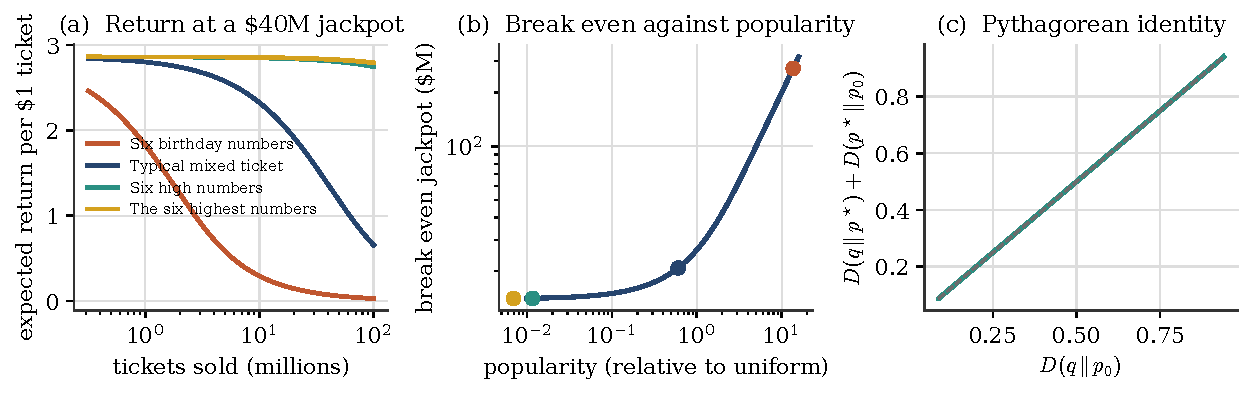
\includegraphics[width=\textwidth]{fig_lottery_return}
\caption{(a) Expected return \eqref{eq:me-return} against tickets sold at a \$40M
jackpot. (b) The jackpot needed to break even, against popularity; markers are the
tickets of Table~\ref{tab:me-lottery}. (c) The Pythagorean identity of
Theorem~\ref{thm:me-tilt}(ii), which underlies every projection onto an affine set in this section.}
\label{fig:me-return}
\end{figure}

Table~\ref{tab:me-lottery} evaluates \eqref{eq:me-return} (plotted in Figure~\ref{fig:me-return}) at $N=20$ million under the synthetic marginals of Figure~\ref{fig:me-lottery}(a), so it illustrates the mechanism rather than measuring Lotto 6/49. The
spread is driven entirely by co-winner dilution. Six ``birthday'' numbers are
over-played fourteenfold and need a \$273M jackpot to break even; the six highest
numbers are under-played more than a hundredfold and break even at \$14.1M.

\begin{table}[htbp]
\centering\small
\begin{tabular}{@{}lrrr@{}}
\toprule
Ticket & Popularity & $\E[\text{return}]$, \$40M pot & Break-even jackpot \\
\midrule
Six birthday numbers ($\le31$) & $13.66\times$ & \$0.15 & \$273.2M \\
Typical mixed ticket & $0.60\times$ & \$1.92 & \$20.9M \\
Six high numbers ($>31$) & $0.012\times$ & \$2.84 & \$14.1M \\
The six highest numbers & $0.007\times$ & \$2.85 & \$14.1M \\
\bottomrule
\end{tabular}
\caption{Parimutuel expected return on a \$1 ticket under the distribution fitted to the synthetic marginals of Figure~\ref{fig:me-lottery}(a), $N=20$M
tickets sold.}
\label{tab:me-lottery}
\end{table}

\paragraph{Two caveats, both theirs.}
Equation \eqref{eq:me-return} ignores lower prize tiers and taxes, which shift
the level. More importantly, the maximum entropy law is a
model of \emph{ignorance}, not of bettors: it is the least committal distribution
consistent with the marginals. The product form \eqref{eq:me-condbern} admits no
interaction between numbers, whereas real players trace patterns on the play-slip,
which marginals cannot see. Stern and Cover found that the maximum entropy law badly underestimates how often the most popular tickets are chosen. The
honest conclusion is that the marginals bound the popularity effect rather than
pin it down.

%---------------------------------------------------------------------
\subsection{Fixed Baseline, Inequality Constraints: Dykstra--Bregman}
\label{sec:me-dykstra}

Relax equality to inequality and the cell changes character. Let
$\mathcal{C}=\{p\in\Delta : Ap\le b,\ Bp=c\}$ be polyhedral.

\paragraph{The tilt survives; the multiplier does not.}
The KKT conditions give
\begin{equation}
\label{eq:me-kkt}
 p^\star(x)=\frac{p_0(x)\exp\{-\mu^\top A_{\cdot x}-\nu^\top B_{\cdot x}\}}{Z(\mu,\nu)},
 \qquad \mu\ge0,\qquad \mu_j (Ap^\star-b)_j = 0 .
\end{equation}

\begin{figure}[htbp]
\centering
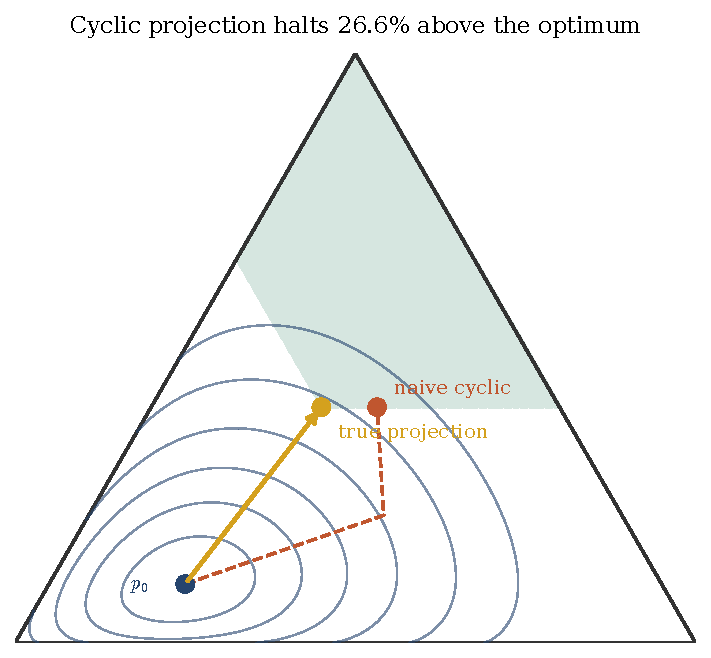
\includegraphics[width=0.62\textwidth]{fig_cyclic_fails}
\caption{$I$-projection onto the intersection of two half-spaces in the simplex on three points.
Naive cyclic $I$-projection halts at the first feasible point it reaches. That
point is feasible, and its relative entropy to $p_0$ is 26.6\% above the optimum.
Dykstra--Bregman recovers the true $I$-projection given by \eqref{eq:me-kkt}. For
affine constraints the naive cycle would be correct
(Theorem~\ref{thm:me-cyclic}); the failure is caused entirely by the
inequalities.}
\label{fig:me-cyclic}
\end{figure}

Only the \emph{active} inequalities tilt the baseline; inactive ones contribute
nothing, by complementary slackness. This is a break from the affine case,
where every constraint binds by construction, and it is what breaks the
cycle.

\paragraph{Naive cycling is wrong.}
Once an iterate lies strictly inside $\mathcal{C}_k$, the $I$-projection onto
$\mathcal{C}_k$ is the identity, its multiplier is zero, and the cycle stops making
progress on that constraint even when the optimum lies on its boundary. The
algorithm halts at the first jointly feasible point it reaches. That point
satisfies every constraint, and it is not $p^\star$.

\paragraph{The correction.}
Dykstra's algorithm with Bregman projections
(Bregman, 1967; Dykstra, 1985; Censor and Reich, 1998; Bauschke and Lewis, 2000) stores, for each
set, the tilt that was \emph{not} applied and reintroduces it on the next pass:
\[
 p^{(t)}=\Pi^{\KL}_{\mathcal{C}_k}\big(p^{(t-1)}\odot z_k^{(t-1)}\big),
 \qquad
 z_k^{(t)}=z_k^{(t-1)}\odot p^{(t-1)}/p^{(t)} .
\]
This restores the Pythagorean bookkeeping and converges to $p^\star$. For
half-spaces each projection is a one-dimensional dual root-find, so the cost is
negligible. Alternatively solve the dual
$\sup_{\mu\ge0,\nu}\{-\mu^\top b-\nu^\top c-\log Z(\mu,\nu)\}$ directly: concave,
with a simple nonnegativity constraint, so L-BFGS-B suffices in moderate
dimension.

\begin{remark}
IPF is the equality special case of Dykstra--Bregman, not a method that happens to
generalize. Applied work that raises inequality constraints and reaches for
iterative scaling is making an error its output will not reveal.
\end{remark}

%---------------------------------------------------------------------
\subsection{Self-Consistent Baseline: Blahut--Arimoto}
\label{sec:me-blahut}

Change one thing: let the baseline be the marginal induced by the rule itself. The
problem stops being a projection onto a constraint set and becomes a saddle
problem over a channel. This cell is where rate--distortion, rational inattention,
and entropy-regularized prediction all live.

The following identity is what turns rate--distortion from a constrained
optimization over channels into an alternating minimization over a product set. It
is the reason Blahut--Arimoto exists.

\begin{lemma}[The marginal is a minimizer]
\label{lem:me-marginal}
For any channel $q(y\mid x)$ and any distribution $m$ on $\mathcal{Y}$,
\begin{equation}
\label{eq:me-marginal}
 I(X;Y) = \min_m \sum_x p(x)\, D\big(q(\cdot\mid x)\,\|\,m\big),
\end{equation}
with the minimum attained uniquely at $m^\star(y)=\sum_x p(x)q(y\mid x)$, the
induced marginal.
\end{lemma}

\begin{proof}
Write $\bar q=m^\star$. For any $m$,
\[
 \sum_x p(x)D(q(\cdot\mid x)\|m) - \sum_x p(x)D(q(\cdot\mid x)\|\bar q)
 = \sum_y \bar q(y)\log\frac{\bar q(y)}{m(y)} = \D{\bar q}{m} \ge 0,
\]
with equality only at $m=\bar q$. The value at $\bar q$ is $I(X;Y)$ by definition.
\end{proof}

Lemma~\ref{lem:me-marginal} says the mutual information is \emph{already} a
minimum, so the rate--distortion problem $\min_q\{I(X;Y)+\lambda\E[d]\}$ is
a minimization over $q$ of a minimization over $m$, hence a joint minimization of
\begin{equation}
\label{eq:me-F}
 F(q,m) = \sum_{x,y} p(x)q(y\mid x)\log\frac{q(y\mid x)}{m(y)}
 + \lambda\sum_{x,y} p(x) q(y\mid x) d(x,y)
\end{equation}
over the product of channels and marginals. $F$ is jointly convex, and each
coordinate problem has a closed form: the $q$-step by
Theorem~\ref{thm:me-tilt}(i) and the $m$-step by Lemma~\ref{lem:me-marginal}. That
is Theorem~\ref{thm:me-csiszar-tusnady}, because $F(q,m)$ is the relative entropy of the joint law $p(x)q(y\mid x)$ to the finite measure $p(x)m(y)e^{-\lambda d(x,y)}$, and the two updates \eqref{eq:me-BA} are
simply those two closed forms written out.

\subsubsection{The two canonical problems}

\paragraph{Capacity (Arimoto, 1972).}
For a fixed channel $Q(y\mid x)$, maximize $I(X;Y)$ over the input $p$. The
variational identity
$I(p,Q)=\max_r \sum_{x,y} p(x)Q(y\mid x)\log\{r(x\mid y)/p(x)\}$, attained at the
Bayes posterior, gives
\[
\begin{aligned}
 r^{(t+1)}(x\mid y)&=\frac{p^{(t)}(x)Q(y\mid x)}{\sum_{x'} p^{(t)}(x')Q(y\mid x')},\\
 p^{(t+1)}(x)&\propto \exp\Big\{\sum_y Q(y\mid x)\log r^{(t+1)}(x\mid y)\Big\}.
\end{aligned}
\]

\paragraph{Rate--distortion (Blahut, 1972).}
For a fixed source $p(x)$ and distortion $d(x,y)$, minimize
$I(X;Y)+\lambda\E[d]$ over channels:
\begin{equation}
\label{eq:me-BA}
 q^{(t+1)}(y\mid x)=\frac{m^{(t)}(y)e^{-\lambda d(x,y)}}{\sum_{y'} m^{(t)}(y')e^{-\lambda d(x,y')}},
 \qquad
 m^{(t+1)}(y)=\sum_x p(x)\,q^{(t+1)}(y\mid x).
\end{equation}
Both are Theorem~\ref{thm:me-csiszar-tusnady} for a relative entropy against finite measures: for rate--distortion $\mathcal{C}_1$ holds the channels
and $\mathcal{C}_2$ the marginals, through $F$ of \eqref{eq:me-F}, and for capacity $\mathcal{C}_1$ holds the inputs $p$ and $\mathcal{C}_2$ the backward channels $r$, through $\D{p(x)Q(y\mid x)}{r(x\mid y)Q(y\mid x)}$, the negative of the objective maximized above.

\begin{figure}[htbp]
\centering
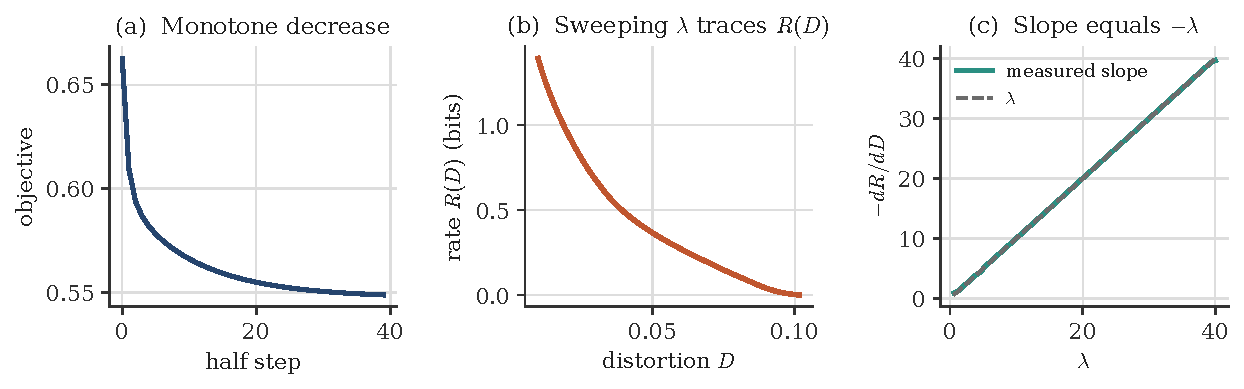
\includegraphics[width=\textwidth]{fig_blahut_verified}
\caption{Blahut--Arimoto, verified. (a) The objective decreases monotonically at
every half-step; there is no step size. (b) Sweeping $\lambda$ traces $R(D)$.
(c) The frontier slope equals $-\lambda$ to within numerical gradient error, as the
first-order condition requires.}
\label{fig:me-blahut}
\end{figure}

\subsubsection{The fixed point is the Gibbs rule}

\begin{proposition}
\label{prop:me-gibbs}
Put $U(x,y)=-d(x,y)$ in \eqref{eq:me-BA}. The fixed point is
\[
 q^\star(y\mid x)=\frac{\bar q^\star(y)e^{\lambda U(x,y)}}{Z_\lambda(x)},
 \qquad
 \bar q^\star(y)=\sum_x p(x)q^\star(y\mid x),
\]
with $Z_\lambda(x)=\sum_y\bar q^\star(y)e^{\lambda U(x,y)}$ and optimal value $-\E[\log Z_\lambda(X)]$; equivalently, $\lambda^{-1}\E[\log Z_\lambda(X)]$ is the maximum of $\E[U]-\lambda^{-1}I(X;Y)$.
\end{proposition}

This is the Gibbs predictive rule of entropy-regularized prediction,
self-consistent marginal and all. Three consequences matter for practice.

\begin{enumerate}
 \item \emph{Blahut--Arimoto is the algorithm, not mirror descent.} Mirror descent
 with step sizes reproduces only the first half of \eqref{eq:me-BA}; the marginal
 update is the missing half. BA needs no step size and is monotone by
 Theorem~\ref{thm:me-csiszar-tusnady}. Mirror descent is the fallback when the
 rule is restricted to a parametric family, which is \S\ref{sec:me-mm}.
 \item \emph{The efficiency frontier is $R(D)$.} The (mutual information, risk)
 frontier is a rate--distortion curve: convex and non-increasing by theorem, with
 slope $-\lambda$ at each point. We verify the slope to within 4.8\% numerical
 gradient error (Figure~\ref{fig:me-blahut}).
 \item \emph{Calibration to an information budget is an $R(D)$ sweep.} Solving
 $I(q^\star_\lambda)=\kappa$ is one BA run per $\lambda$ plus a monotone
 one-dimensional root-find.
\end{enumerate}

\subsubsection{Sims's rational inattention}
\label{sec:me-sims}

The clearest economic use of a self-consistent baseline is the theory of rational
inattention (Sims, 2003; Sims, 2006; Sims, 2010; for a review see Ma\'ckowiak, Mat\v{e}jka and Wiederholt, 2023). An agent may condition actions on
the state only through a channel of finite Shannon capacity: choose the joint law
of state and action to maximize expected payoff subject to $I(\omega;a)\le\kappa$.
That is \eqref{eq:me-BA} with the agent's loss in the role of distortion. Sims's
capacity constraint \emph{is} a rate--distortion constraint, and Blahut--Arimoto
is its solver. This is not always recognized.

\paragraph{Linear--quadratic tracking: attention is all-or-nothing.}
Let $x\sim\N(0,\Sigma)$ and let the agent choose $a$ to minimize
$\E\|x-a\|^2$ under the capacity constraint. Gaussian in, Gaussian out,
and in the eigenbasis of $\Sigma$ with $\sigma_1^2\ge\cdots\ge\sigma_d^2$ the
solution is \emph{reverse water-filling}:
\begin{equation}
\label{eq:me-waterfill}
 v_i=\min(\theta,\sigma_i^2),\qquad
 R(\theta)=\sum_i \max\Big\{0,\tfrac12\log_2\frac{\sigma_i^2}{\theta}\Big\},\qquad
 D(\theta)=\sum_i \min(\theta,\sigma_i^2),
\end{equation}
with $\theta$ set by $R(\theta)=\kappa$. The economic content is sharper than the
usual reading of rational inattention as ``everything observed a little noisily.''
Directions with $\sigma_i^2\le\theta$ receive \emph{exactly zero} bits. They are
not tracked imprecisely. They are not tracked.

\begin{figure}[htbp]
\centering
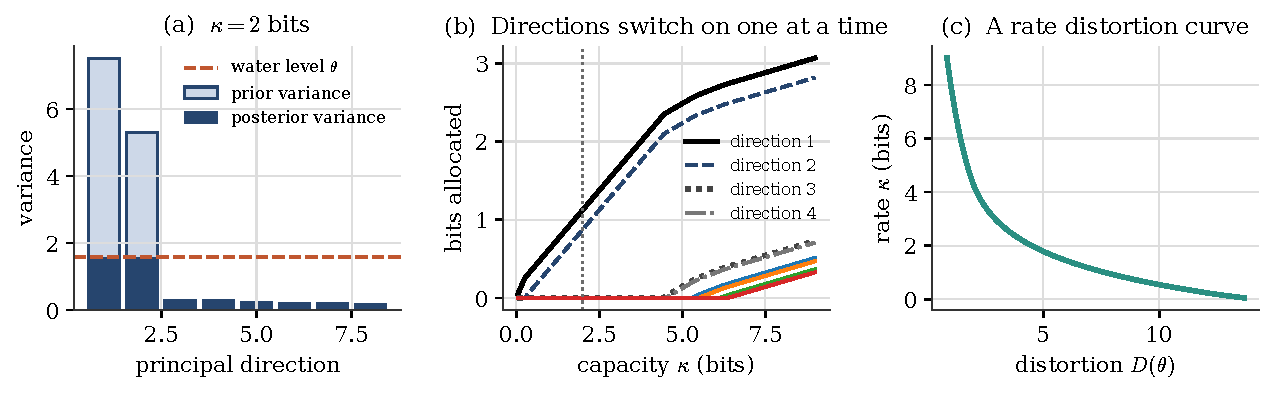
\includegraphics[width=\textwidth]{fig_sims_waterfilling}
\caption{Sims (2003) as reverse water-filling for an eight variable state with two common
factors. (a) Prior variances by principal direction; the water level $\theta$ is set by
capacity. At $\kappa=2$ bits, six of eight directions receive zero bits. (b) Directions
switch on one at a time as capacity grows, the two factor directions first. (c) Equation
\eqref{eq:me-waterfill} is a rate--distortion curve.}
\label{fig:me-sims}
\end{figure}

Figure~\ref{fig:me-sims} takes an eight-variable state with a two-factor
covariance, the structure of a factor model of sectoral shocks. At $\kappa=2$ bits
the water level is $\theta=1.58$; the agent spends 1.13 bits on the first
principal direction and 0.87 on the second, and ignores six of the eight
directions entirely. The loss is 4.50 against a prior variance of 14.16, so two
bits buy back 68\% of the uncertainty, because the factor structure concentrates
it in two directions. As $\kappa$ rises directions switch on one at a time: attention is allocated at
the extensive margin first and the intensive margin second.

\paragraph{Discrete choice: logit without Gumbel, and endogenous consideration sets.}
Outside the linear--quadratic world one must compute. Mat\v{e}jka and McKay (2015)
study an inattentive consumer choosing among $J$ products with payoff
$u(a,\omega)$, prior $\mu$, and price $\lambda$ per nat. The first-order
conditions are
\begin{equation}
\label{eq:me-matejka}
 P(a\mid\omega)=\frac{P_0(a)e^{u(a,\omega)/\lambda}}{\sum_b P_0(b)e^{u(b,\omega)/\lambda}},
 \qquad
 P_0(a)=\sum_\omega \mu(\omega)P(a\mid\omega).
\end{equation}
Compare \eqref{eq:me-matejka} with \eqref{eq:me-BA}: the same pair of equations,
with $P_0$ the self-consistent marginal and $1/\lambda$ here in the role of $\lambda$ there. Two consequences.

First, \eqref{eq:me-matejka} is a multinomial logit with inverse temperature
$1/\lambda$, arising from an information cost rather than from Gumbel errors
(McFadden, 1974). Entropy-regularized prediction reaches the same form from
coherence axioms, and Section~\ref{ch:sanov} reaches it from conditioning. Three
unrelated routes, one functional form.

Second, $P_0$ is neither free nor uniform. It is determined in equilibrium, and at
the optimum some of its entries are zero: a product of low enough baseline
appeal drops out of the choice set entirely, and no state of the world will make
the agent buy it. Standard logit cannot predict this; Blahut--Arimoto produces it
without being asked. In Figure~\ref{fig:me-matejka}, six products have baseline
appeals $1.00, 0.90, 0.75, 0.50, 0.25, 0.00$, and the state of the world adds an
independent shock of $\pm0.5$ to each, giving sixty four equiprobable states. Product 6, whose payoff never exceeds that of product 1 in any state, is never considered, since $G(6)<G(1)\le1$ in the notation of \eqref{eq:me-G} below. The other
products leave the consideration set in exact reverse order of appeal, at
\[
 \lambda=0.085,\ 0.220,\ 0.639,\ 2.483 \quad \text{(products 5, 4, 3, 2)},
\]
while product 1 is always considered. At $\lambda=0.05$ the agent extracts 1.13
nats and tracks the state closely, as the near deterministic channel in panel (d)
shows. At $\lambda=1.5$ two products survive, the agent extracts 0.02 nats, and
the choice is almost independent of the state.

\begin{figure}[htbp]
\centering
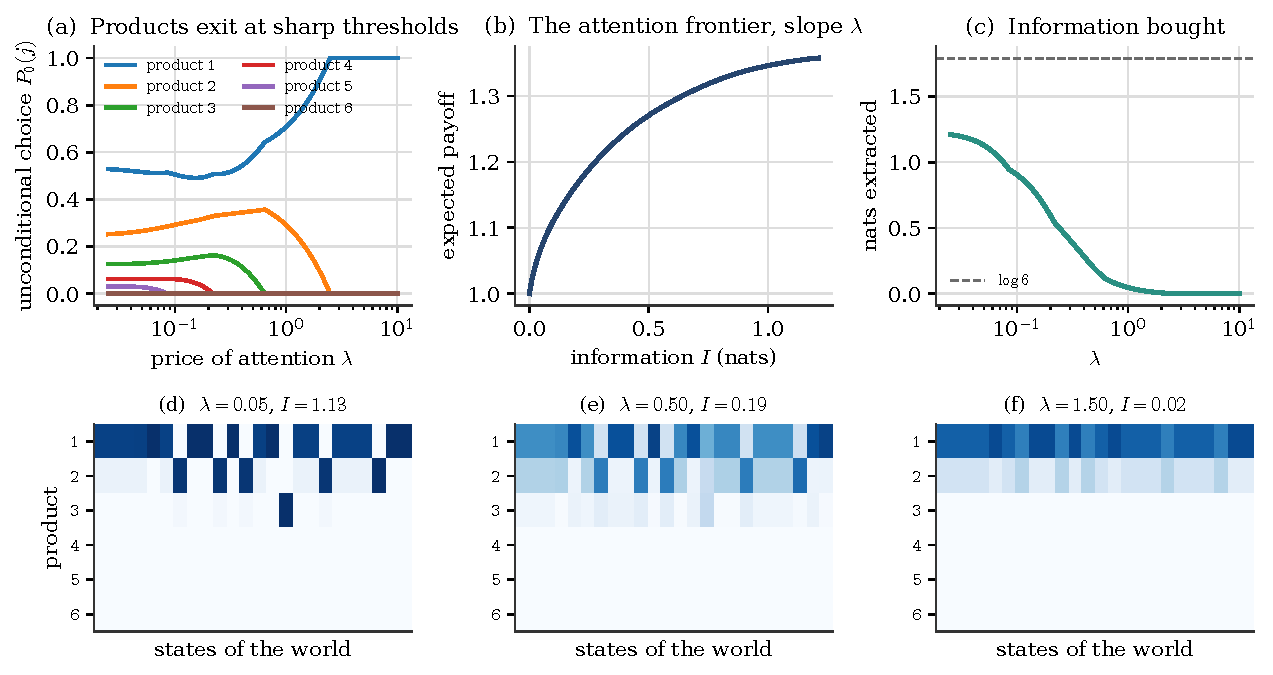
\includegraphics[width=\textwidth]{fig_matejka_mckay}
\caption{Mat\v{e}jka and McKay (2015) computed by Blahut--Arimoto. (a)
Unconditional choice probabilities against the price of attention; products exit
the consideration set at sharp thresholds in reverse order of appeal. (b) The
attention frontier, of slope $\lambda$. (c) Information bought against its price.
(d) to (f) The channel $P(j\mid\omega)$ at three prices: nearly deterministic when
attention is cheap, nearly state independent when it is dear.}
\label{fig:me-matejka}
\end{figure}

\subsubsection{Shutdown is complementary slackness}

The two cases share more than a family resemblance. In both, an inequality
constraint goes active and the corresponding object is switched off entirely. We
prove this, because it is the claim on which the unity of the section rests, and
because it shows that the shutdown in both problems is complementary slackness, the mechanism of the inequality-constrained
$I$-projection of \S\ref{sec:me-dykstra}.

\begin{proposition}[Water-filling is KKT]
\label{prop:me-waterfill-kkt}
In the LQG problem, the optimal posterior variances solve
$\min_v \sum_i \tfrac12\log(\sigma_i^2/v_i)$ subject to $\sum_i v_i\le D$ and
$v_i\le\sigma_i^2$. With multipliers $\mu\ge0$ on the distortion budget and
$\nu_i\ge0$ on $v_i\le\sigma_i^2$, stationarity gives
$-1/(2v_i)+\mu+\nu_i=0$. Hence
\[
 \nu_i=0 \implies v_i=\tfrac{1}{2\mu}=:\theta,
 \qquad
 \nu_i>0 \implies v_i=\sigma_i^2 \text{ and } \sigma_i^2\le\theta,
\]
which is \eqref{eq:me-waterfill}. Direction $i$ receives zero bits if and only if
the constraint $v_i\le\sigma_i^2$ is active.
\end{proposition}

So the ignored directions are not a curiosity of the Gaussian algebra. They are
the active set.

\begin{proposition}[Consideration sets are KKT]
\label{prop:me-consideration}
In the discrete problem,
$\partial I/\partial P(a\mid\omega)=\mu(\omega)\log\{P(a\mid\omega)/P_0(a)\}$, the
dependence of $I$ on $P_0$ canceling as in the proof, at the end of this section, that mutual information is convex in the channel.
Attaching multipliers $\zeta(\omega)$ to $\sum_a P(a\mid\omega)=1$ and
$\nu(a,\omega)\ge0$ to $P(a\mid\omega)\ge0$, stationarity yields
\eqref{eq:me-matejka} on the support. Define
\begin{equation}
\label{eq:me-G}
 G(a)=\sum_\omega \mu(\omega)\frac{e^{u(a,\omega)/\lambda}}{Z_\lambda(\omega)},
 \qquad
 Z_\lambda(\omega)=\sum_b P_0(b)e^{u(b,\omega)/\lambda}.
\end{equation}
Then substituting \eqref{eq:me-matejka} into
$P_0(a)=\sum_\omega \mu(\omega)P(a\mid\omega)$ gives $P_0(a)=P_0(a)G(a)$, so that the first implication below holds; the second, where the substitution reads $0=0$, is the KKT condition for $P_0(a)\ge0$ in the reduced problem $\max_{P_0}\sum_\omega\mu(\omega)\log Z_\lambda(\omega)$ (Lemma~\ref{lem:me-marginal} and Proposition~\ref{prop:me-envelope}), whose objective is concave in $P_0$ with gradient $G$:
\[
 P_0(a)>0 \implies G(a)=1,
 \qquad
 P_0(a)=0 \implies G(a)\le1 .
\]
Action $a$ lies outside the consideration set if and only if the constraint
$P_0(a)\ge0$ is active, with multiplier $1-G(a)\ge0$.
\end{proposition}

\begin{table}[htbp]
\centering
\begin{tabular}{@{}lrrrrrr@{}}
\toprule
 & P1 & P2 & P3 & P4 & P5 & P6 \\
\midrule
\multicolumn{7}{@{}l}{$\lambda=0.6$: three products considered}\\
$P_0(a)$ & 0.625 & 0.355 & 0.020 & 0 & 0 & 0 \\
$G(a)$ & 1.000 & 1.000 & 1.000 & 0.668 & 0.441 & 0.290 \\
\addlinespace
\multicolumn{7}{@{}l}{$\lambda=1.5$: two products considered}\\
$P_0(a)$ & 0.805 & 0.195 & 0 & 0 & 0 & 0 \\
$G(a)$ & 1.000 & 1.000 & 0.925 & 0.783 & 0.663 & 0.561 \\
\bottomrule
\end{tabular}
\caption{The consideration set is an active set. $G(a)$ is defined in
\eqref{eq:me-G}.}
\label{tab:me-consideration}
\end{table}

Table~\ref{tab:me-consideration} checks this on the example of
Figure~\ref{fig:me-matejka}. Every product inside the consideration set has
$G(a)=1$ to six decimals; every product outside it has $G(a)<1$. The multiplier
$1-G(a)$ vanishes continuously at the threshold, which is why the exits in
Figure~\ref{fig:me-matejka}(a) are sharp without being discontinuous.

Propositions~\ref{prop:me-waterfill-kkt} and~\ref{prop:me-consideration} say the
same thing twice. A direction of the state and an item on a menu are both switched
off exactly when a nonnegativity constraint binds, and the multiplier on that
constraint is the shadow value of relaxing it. Finite capacity does not spread
itself thinly over everything. It buys a few things and ignores the rest, and the
cut-off is an active set, fixed by complementary slackness as in \eqref{eq:me-kkt}. That is why
\S\ref{sec:me-dykstra} is not a digression, although rational inattention stays in the
self-consistent equality cell of the taxonomy: the inequalities that switch things off are nonnegativity
constraints, which the Blahut--Arimoto update respects without being told.

\paragraph{What $\lambda$ means.}
A question entropy-regularized prediction invites but does not settle: what does
$\lambda$ mean? It is not a tuning constant. Its reciprocal, the $\lambda$ of \eqref{eq:me-matejka}, is the shadow price of
information, in payoff units per nat, and $-\lambda$ is the slope of the frontier $R(D)$.
Cross-validation may select it; its interpretation is economic.

%---------------------------------------------------------------------
\subsection{Parametric Families: Majorization}
\label{sec:me-mm}

Blahut--Arimoto is exact only when $q$ ranges over all channels. Restrict to a
parametric family $q_\theta$, as every application does, and the channel
half-step leaves the family. The standard response is mirror descent with a step
size. The better response is majorize--minorize
(Lange, Hunter and Yang, 2000; Hunter and Lange, 2004): replace the objective by a quadratic
minorant touching it at the current iterate, maximize the minorant in closed form,
repeat. This is the alternating scheme of \S\ref{sec:me-alternating} with $\mathcal{C}_1$ the
surrogate and $\mathcal{C}_2$ the parameter space, and it is monotone for the same
reason as EM, although Theorem~\ref{thm:me-csiszar-tusnady} does not apply as stated.

\begin{lemma}[Bouchard, 2007]
\label{lem:me-bouchard}
For any $\alpha\in\R$ and $u,\xi\in\R^J$, with $z_j=u_j-\alpha$ and
$\varphi(\xi)=\tanh(\xi/2)/(4\xi)$,
\begin{equation}
\label{eq:me-bouchard}
 \log\sum_{j=1}^J e^{u_j} \;\le\; \alpha+\sum_{j=1}^J
 \Big[\tfrac12(z_j-\xi_j)+\varphi(\xi_j)\big(z_j^2-\xi_j^2\big)+\log\big(1+e^{\xi_j}\big)\Big],
\end{equation}
with the right side minimized over $\xi$ at $\xi_j=|u_j-\alpha|$ and over $\alpha$ at the solution of
\[
\alpha=\{(J/2-1)+2\sum_j\varphi(\xi_j)u_j\}/\{2\sum_j\varphi(\xi_j)\}.
\]
\end{lemma}

\begin{proof}
Two steps. From $\prod_j(1+a_j)\ge1+\sum_j a_j$ for $a_j\ge0$,
$\log\sum_j e^{u_j}\le\alpha+\sum_j\log(1+e^{u_j-\alpha})$. Then apply the
Jaakkola and Jordan (2000) bound
$\log(1+e^z)\le\tfrac12(z-\xi)+\varphi(\xi)(z^2-\xi^2)+\log(1+e^\xi)$ termwise.
\end{proof}

The bound is quadratic in $u$, hence in $\theta$ when $u_j=x^\top\theta_j$, so each
MM step is a weighted least squares. B\"ohning and Lindsay (1988) and
B\"ohning (1992) go further and remove the dependence on $\theta$ altogether: with $\ell$ the average log-likelihood of the logit (the utility term) and $H_U(\theta)=-\nabla^2_\theta\ell(\theta)$ its curvature,
\begin{equation}
\label{eq:me-bohning}
 H_U(\theta) \preceq B := \tfrac12\Big[I_{J-1}-\tfrac1J \mathbf{1}\mathbf{1}^\top\Big]
 \otimes \tfrac1n X^\top X \quad\text{for all }\theta,
\end{equation}
so that $\theta^{t+1}=\theta^t+B^{-1}\nabla\ell(\theta^t)$ ascends monotonically
using one matrix factorization for the entire run. We verify
\eqref{eq:me-bouchard} at $10^5$ random $(u,\alpha,\xi)$ with $J=4$, where the slack is never
negative, and \eqref{eq:me-bohning} at 400 standard normal $\theta$ in a logit with $J=4$, $n=200$ and $d=9$ standard normal covariates, where
$\lambda_{\min}(B-H_U)$ never falls below $5.3\times10^{-2}$. Newton with an
aggressive step is not monotone; MM is, unconditionally.

%---------------------------------------------------------------------
\subsection{The Gibbs Rule is a Proximal Operator}
\label{sec:me-prox}

Sections \ref{sec:me-ipf}--\ref{sec:me-mm} gave four algorithms. This section
explains, in one line of convex duality, why they are the same algorithm, and
\S\ref{sec:me-curvature} then uses that line to fix something.

\begin{proposition}[The log-partition is the entropic envelope]
\label{prop:me-envelope}
For a baseline $\bar q$ on $\mathcal{Y}$ and a utility vector
$u\in\R^{|\mathcal{Y}|}$,
\begin{equation}
\label{eq:me-logZ}
 \log Z(u)=\log\sum_y \bar q(y)e^{u_y}
 = \sup_{q\in\Delta(\mathcal{Y})}\Big\{\langle u,q\rangle - \D{q}{\bar q}\Big\},
 \qquad \nabla_u \log Z(u)=q^\star,
\end{equation}
where $q^\star$ is the Gibbs rule.
\end{proposition}

Read \eqref{eq:me-logZ} slowly. The log-partition function is the Fenchel
conjugate of relative entropy, and the Gibbs rule is its gradient. As a minimization, the same identity makes $-\log Z(u)$ the entropic envelope of the linear loss $-\langle u,\cdot\rangle$ at $\bar q$ and the Gibbs rule,
its minimizer, the entropic proximal map of that loss. The optimal value of Proposition~\ref{prop:me-gibbs}, in its maximization form
$\lambda^{-1}\E[\log Z_\lambda(X)]$, is therefore, up to sign, an entropic envelope
evaluated in expectation, not an incidental formula. We verify \eqref{eq:me-logZ}
numerically: over 200 random draws a generic optimizer matches the supremum to $2\times10^{-13}$, and central differences match the gradient to $4\times10^{-10}$.

\subsubsection{What a proximal operator is, and why one wants it}

Take a convex function $f$ that is awkward: nonsmooth, or constrained, or defined only
implicitly. Moreau's construction (Moreau, 1965; see Parikh and Boyd, 2014) replaces it by
\[
 e_\gamma f(x)=\min_z\Big\{f(z)+\tfrac{1}{2\gamma}\|x-z\|^2\Big\},
 \qquad
 \mathrm{prox}_{\gamma f}(x)=\arg\min_z\Big\{f(z)+\tfrac{1}{2\gamma}\|x-z\|^2\Big\},
\]
the envelope and the proximal map. Two facts make this worth doing. The envelope
$e_\gamma f$ is differentiable even when $f$ is not, and it has the same
minimizers. And its gradient is
$\nabla e_\gamma f(x)=\{x-\mathrm{prox}_{\gamma f}(x)\}/\gamma$, so computing the
prox and computing the gradient of the smoothed problem are the same act.

Now read \eqref{eq:me-logZ} again. The awkward function is relative entropy, which
is constrained (its argument must be a probability vector) and its gradient blows up at the
boundary. Its Fenchel conjugate is the log-partition $\log Z$: smooth, unconstrained, convex,
defined on all of $\R^{|\mathcal{Y}|}$, with the softmax as its gradient by Danskin. Taken with respect to the Bregman geometry rather than the
Euclidean one, the same identity makes $-\log Z$ the envelope, and the softmax the proximal map, of the linear loss $-\langle u,\cdot\rangle$ at $\bar q$
(not of relative entropy, whose entropic proximal map is a geometric mixture). So:

\begin{quote}
The Gibbs rule is not merely \emph{like} a proximal operator. It \emph{is} one.
\end{quote}

This has content beyond bookkeeping. It says that everything known about proximal
algorithms transfers: that the fixed point is characterized by a zero of a
monotone operator; that the iteration is firmly nonexpansive in the right metric, which is
why it cannot cycle; that acceleration schemes apply; and that splitting methods
let one handle a sum of penalties by handling each separately. It also explains an
otherwise curious fact about Blahut--Arimoto, namely that the algorithm never
overshoots. Proximal maps are firmly nonexpansive. There is nothing to overshoot
with.

The practical corollary is worth repeating, because it is the most actionable
sentence in the section. If the predictive rule is unrestricted, do not run mirror
descent. Mirror descent is the inexact entropic prox, obtained by linearizing $f$
before taking the step, and the linearization is what forces a step size back into
the problem. Blahut takes the step exactly. The only reason to linearize is that
one cannot solve the inner problem, and here one can.

\subsubsection{The entropic prox}

Replacing Moreau's quadratic by a Bregman divergence gives the entropic proximal
operator (Teboulle, 1992; Censor and Zenios, 1992; Chen and Teboulle, 1993; Eckstein, 1993),
\[
 \mathrm{prox}^D_{\gamma f}(q^t)
 = \arg\min_q\Big\{f(q)+\gamma^{-1}D\big(q\,\|\,q^t\big)\Big\}.
\]
When $f$ is linear this is the exponentiated-gradient step; as $\gamma\to\infty$ it
is exact minimization. \emph{Blahut's $q$-step is the exact entropic prox}, which
is why it needs no step size: the three-point property of the Bregman divergence
does the work a line search would otherwise do. Mirror descent
(Nemirovski and Yudin, 1983; Beck and Teboulle, 2003) is its inexact version.
Polson, Scott and Willard (2015) survey statistical algorithms as this
envelope--gradient pair, and our framework is an instance: the information penalty
is the Bregman potential, the Gibbs rule is the prox, the log-partition is the
envelope, and Blahut--Arimoto is proximal point in KL geometry.

%---------------------------------------------------------------------
\subsection{Mixtures and Envelopes}
\label{sec:me-mixenv}

Bouchard's bound is one half of a duality. The other half is data augmentation\index{data augmentation}.

\paragraph{Envelope.}
Write a term as an infimum over a latent scale,
$\phi(\psi)=\inf_\omega\{\tfrac12\omega\psi^2+g(\omega)\}$. Minimizing out $\omega$
yields a quadratic surrogate: MM, variational Bayes, Jaakkola--Jordan, Bouchard.
Deterministic.

\paragraph{Mixture.}
Write the same term as an integral,
$e^{-\phi(\psi)}=\int e^{-\omega\psi^2/2}p(\omega)\,d\omega$. For the logistic
likelihood this is P\'olya--Gamma augmentation (Polson, Scott and Windle, 2013),
\[
 \frac{(e^\psi)^a}{(1+e^\psi)^b}
 = 2^{-b}e^{\kappa\psi}\int_0^\infty e^{-\omega\psi^2/2}p(\omega\mid b,0)\,d\omega,
 \qquad \kappa=a-b/2,
\]
with $\omega\mid\psi\sim\mathrm{PG}(b,\psi)$. Augmenting with $\omega$ gives a
conditionally Gaussian model: EM and MCMC. Stochastic.

They are one construction. Polson and Scott (2016) make this precise as
\emph{hierarchical duality}: the mixture and envelope representations are Fenchel
conjugates, related by Laplace's method. The variational bound is the saddlepoint
approximation to the mixture integral; the mixture integral is the
finite-temperature smoothing of the bound. The governing identity, for $f$ continuous and bounded below on an open set with $\int e^{-f/\varepsilon_0}\,d\omega<\infty$ for some $\varepsilon_0>0$ (the Laplace principle), is
\begin{equation}
\label{eq:me-temperature}
 -\varepsilon\log\int e^{-f(\omega)/\varepsilon}\,d\omega \;\longrightarrow\;
 \inf_\omega f(\omega), \qquad \varepsilon\downarrow0 .
\end{equation}

\emph{Integration and minimization are the same operation at different
temperatures.} That single line explains why Sanov's rate function is the Legendre
conjugate of a cumulant generating function (Section~\ref{ch:sanov}), why the
log-partition is an envelope (\S\ref{sec:me-prox}), and why the Gibbs rule
concentrates on the utility maximizer as the price of information falls
(\S\ref{sec:me-blahut}). The section has one idea in it, wearing different clothes.

\begin{center}
\begin{tabular}{@{}lll@{}}
\toprule
 & \textbf{Mixture (integrate)} & \textbf{Envelope (minimize)} \\
\midrule
Representation & $\int e^{-\omega\psi^2/2}p(\omega)d\omega$ & $\inf_\omega\{\tfrac12\omega\psi^2+g(\omega)\}$ \\
Latent scale & P\'olya--Gamma $\omega$ & variational $(\alpha,\xi)$ \\
Algorithm & EM, Gibbs sampler\index{Gibbs sampler} & MM, variational Bayes \\
Instance & Polson--Scott--Windle (2013) & Jaakkola--Jordan; Bouchard \\
Curvature & $X^\top\Omega X\succeq0$ & $B\succeq H_U$, eq.~\eqref{eq:me-bohning} \\
Character & stochastic, exact & deterministic, conservative \\
\bottomrule
\end{tabular}
\end{center}

Note the penultimate row. Both representations deliver a positive semidefinite
curvature by construction, and neither is the raw Hessian. That is the content of
\S\ref{sec:me-curvature}.

%---------------------------------------------------------------------
\subsection{The Curvature Decomposition is Not Positive Semidefinite}
\label{sec:me-curvature}

Entropy-regularized prediction (Polson and Zantedeschi, 2025c) diagnoses identification through the decomposition
$H_\lambda(\theta)=H_U(\theta)+\lambda^{-1}H_I(\theta)$ of the curvature of the regularized objective, with $H_U$ as in \eqref{eq:me-bohning} and
$H_I(\theta)=\nabla^2_\theta I_\theta$, asserting that both terms are positive
semidefinite. It then builds an identification floor
$\lambda_{\min}(H_\lambda)\ge\lambda^{-1}\lambda_{\min}(H_I)>0$ and a diagnostic
$\rho=\lambda_{\min}(H_U)/\lambda_{\min}(H_I)$ on that basis.

\subsubsection{The claim fails}

\begin{proposition}
\label{prop:me-notpsd}
$\nabla^2_\theta I_\theta$ need not be positive semidefinite.
\end{proposition}

\begin{proof}
Take $J=2$, let $x=\pm1$ with probability $\tfrac12$ each, and let $q_\theta(1\mid x)=s(\theta x)$ with $s(z)=1/(1+e^{-z})$. The marginal of $Y$ is uniform for every $\theta$, so $I_\theta=\log2+s\log s+(1-s)\log(1-s)$ with $s=s(\theta)$, and differentiating twice gives $I_\theta''=s(1-s)\{1-\theta\tanh(\theta/2)\}$, which is negative for $|\theta|>1.55$; for instance $I_\theta''=-0.055$ at $\theta=2$.
\end{proof}

Mutual information is convex in the channel $q$, not in $\theta$
(proved at the end of this section), and convexity is not preserved under nonlinear
reparametrization. The pullback through the softmax carries a second fundamental
form:
\begin{equation}
\label{eq:me-pullback}
 \nabla^2_\theta I_\theta
 = \underbrace{\Big(\frac{\partial q}{\partial\theta}\Big)^{\!\top}
 \big(\nabla^2_q I\big)
 \Big(\frac{\partial q}{\partial\theta}\Big)}_{\succeq\,0}
 + \underbrace{\sum_k \frac{\partial I}{\partial q_k}\nabla^2_\theta q_k}_{\text{not sign definite}} .
\end{equation}

In the $J=4$ logit of \S\ref{sec:me-mm}, at a standard normal $\theta$,
$\lambda_{\min}(H_U)=+0.0131$ while $\lambda_{\min}(\nabla^2_\theta I_\theta)=-0.0363$,
stable to five decimals across two step sizes. The consequence is not cosmetic:

\begin{center}
\small
\begin{tabular}{@{}lrrrrrrr@{}}
\toprule
$\eta=\lambda^{-1}$ & 0 & 0.5 & 1 & 2 & 5 & 10 & 25 \\
\midrule
$\lambda_{\min}\big(H_U+\eta\nabla^2_\theta I_\theta\big)$
 & $+.0131$ & $+.0067$ & $-.0053$ & $-.0357$ & $-.1399$ & $-.3196$ & $-.8626$ \\
\bottomrule
\end{tabular}
\end{center}

Raising the information price drives the smallest eigenvalue negative. There is no
floor, $H_\lambda$ becomes indefinite, and $\rho<0$, meaningless as a ratio of
precisions. The same text elsewhere describes $H_I$ as ``the Fisher information of
the predictive channel,'' which is a different object, and one that under the log
score simply equals $H_U$, forcing $\rho\equiv1$. The two descriptions are mutually
inconsistent and neither supports the floor.


\subsubsection{The envelope repairs it}

Keep only the first term of \eqref{eq:me-pullback}:
\begin{equation}
\label{eq:me-Henv}
 H^{\mathrm{env}}_I(\theta) :=
 \Big(\frac{\partial q}{\partial\theta}\Big)^{\!\top}
 \big[\nabla^2_q I\big]
 \Big(\frac{\partial q}{\partial\theta}\Big) \;\succeq\; 0
 \qquad\text{by construction.}
\end{equation}
That $\nabla^2_q I\succeq0$ is Cauchy--Schwarz (see the proofs at the end of this section); we
verify $H^{\mathrm{env}}_I\succeq0$ at 300 standard normal $\theta$ in the logit of \S\ref{sec:me-mm}, where its smallest eigenvalue never falls below $4\times10^{-3}$.

Equation \eqref{eq:me-Henv} is not an \emph{ad hoc} patch. It is the
Gauss--Newton curvature of $I_\theta$: it keeps the curvature of $I$ in the coordinates $q$, where $I$ is convex, and drops the second fundamental form of the map $\theta\mapsto q$. It need not be the curvature of a majorizer, since a quadratic lying above $I_\theta$ and touching it at $\theta$ has curvature at least $\nabla^2_\theta I_\theta$, which exceeds $H^{\mathrm{env}}_I$ in every direction where the second term of \eqref{eq:me-pullback} is positive (a majorant built in $q$ and pulled back keeps that term, because it shares the gradient of $I$ at the point of contact). Like the curvatures $B$ and $X^\top\Omega X$ of \S\ref{sec:me-mixenv}, which stand in for $H_U$, it is positive semidefinite by construction; the raw Hessian of $I_\theta$ is not.

\subsubsection{The surrogate curvature diagnostic}

Define the diagnostic on the surrogate curvature,
$\rho^{\mathrm{env}}=\lambda_{\min}(H_U)/\lambda_{\min}(H^{\mathrm{env}}_I)$, defined when $H^{\mathrm{env}}_I\succ0$. It is
nonnegative, it restores the floor and the diagnostic verbatim, and it is cheap,
because it needs only first derivatives of $q$. Moreover \eqref{eq:me-bohning} yields a
one-sided certificate at \emph{no} Hessian evaluation:
\begin{equation}
\label{eq:me-certificate}
 B \succeq H_U \implies
 \rho^{\mathrm{env}} \le \frac{\lambda_{\min}(B)}{\lambda_{\min}(H^{\mathrm{env}}_I)},
\end{equation}
so a small right-hand side \emph{certifies} weak identification using a matrix that
does not depend on $\theta$ at all.

%---------------------------------------------------------------------
\subsection{Discussion}
\label{sec:me-discussion}

\paragraph{What the taxonomy buys.}
The five literatures named at the outset differ in two respects that matter and
several that do not. What matters is whether the baseline is exogenous or
self-consistent, and whether the constraints admit inequalities. What does not
matter is the notation. A practitioner who knows the cell knows the algorithm, its
guarantees, and the meaning of its fixed point.

\paragraph{Three warnings.}
Cyclic $I$-projection is not a general-purpose tool: correct on affine sets, it
fails silently on inequality-constrained ones, and nothing in the output announces
the failure. Mirror descent is not the natural algorithm for a Gibbs rule but the
fallback; where the rule is unrestricted, Blahut--Arimoto is exact and monotone,
and where it is parametric, B\"ohning's bound is monotone with a single
factorization. And the Hessian of mutual information with respect to a parameter is
not always positive semidefinite, so diagnostics built on it are ill-posed.

\paragraph{The duality is the point.}
If one line survives, let it be \eqref{eq:me-temperature}. Read left to right it
turns P\'olya--Gamma into Jaakkola--Jordan, hierarchical models into variational
bounds, and posterior means into proximal operators. Read right to left it turns a
Legendre transform into a partition function and Sanov's rate function into a
cumulant generating function.

\paragraph{Extensions.}
Three are immediate. \emph{Scale mixtures on the baseline}: the shrinkage weight in
a Gibbs-IV estimator (the Gibbs rule applied to instrumental variable regression; Polson and Zantedeschi, 2025c) is set by the ratio of structural to prior precision
$1/\tau^2$; a half-Cauchy on $\tau$ gives the horseshoe and makes the
identification diagnostic a posterior distribution rather than a scalar, which is
the honest object when instrument strength is itself uncertain. (This connects
directly to the federated horseshoe of \S\ref{sec:fed-horseshoe}, where the same
$\tau$ resists a limit law for the same reason.) \emph{Inequalities with a
self-consistent baseline}: the empty cell of our table. Dykstra handles
inequalities with a fixed baseline, Blahut handles a self-consistent baseline with
equalities, and the combination admits no clean alternating scheme we can find; the
fallback is the dual with sign-constrained multipliers. This is the obvious open
computational problem. \emph{A genuine lottery replication}: our reconstruction
uses synthetic marginals more extreme than those Stern and Cover report, and published
marginals would let one test \eqref{eq:me-condbern} against play-slip patterns,
which is where we expect it to fail.

\paragraph{Limitations.}
Theorem~\ref{thm:vcc} is clean on a finite alphabet with i.i.d.\ sampling;
the continuous and dependent cases require conditions we have not stated. The
Bouchard and B\"ohning bounds are conservative, and that conservatism is the price
of monotonicity. And in every application here the maximum entropy law is a model
of ignorance rather than of the world. Stern and Cover were explicit that theirs
was a rough approximation, contradicted in places by the data. That posture is the
correct one and we adopt it.

%---------------------------------------------------------------------
\subsection*{Proofs for this section}

\subsubsection*{Proof of Theorem~\ref{thm:me-tilt}}

Let $p^\star$ be the tilt with $\theta$ chosen so $\E_{p^\star}[T]=t$,
possible because $t$ is in the relative interior; $\theta$ is unique when $\nabla^2\log Z\succ0$, and $p^\star$ is unique in any case, by the last step below. For any
$p\in\mathcal{C}$,
\[
 \D{p}{p^\star}=\sum_x p(x)\log\frac{p(x)}{p_0(x)}
 - \theta^\top\underbrace{\E_p[T]}_{=\,t}+\log Z(\theta)
 = \D{p}{p_0}-\big(\theta^\top t-\log Z(\theta)\big).
\]
The bracket is free of $p$. Evaluating at $p=p^\star\in\mathcal{C}$ gives
$\theta^\top t-\log Z(\theta)=\D{p^\star}{p_0}$, which is (ii). Since
$\D{p}{p^\star}\ge0$ with equality only at $p=p^\star$, (i) follows. Part (iii) is
the same identity read as a Legendre transform, concavity of
$\theta\mapsto\theta^\top t-\log Z(\theta)$ following from convexity of
$\log Z$. \qed

\subsubsection*{Proof of Proposition~\ref{prop:me-envelope}}

The map $q\mapsto\langle u,q\rangle-\D{q}{\bar q}$ is strictly concave on
$\Delta(\mathcal{Y})$ and differentiable on its relative interior. Stationarity of
the Lagrangian
$\langle u,q\rangle-\sum_y q_y\log(q_y/\bar q_y)-\nu(\sum_y q_y-1)$ gives
$u_y-\log(q_y/\bar q_y)-1-\nu=0$, so $q_y\propto \bar q_y e^{u_y}$, the Gibbs rule.
Substituting back, the optimal value is $\log\sum_y \bar q_y e^{u_y}=\log Z(u)$.
Danskin's theorem gives $\nabla_u\log Z(u)=q^\star$. \qed

\subsubsection*{Mutual information is convex in the channel}

Write $I(q)=\sum_x p(x)\sum_j q_j(x)\log\{q_j(x)/\bar q_j\}$ with
$\bar q_j=\sum_x p(x)q_j(x)$. Then
$\partial I/\partial q_j(x)=p(x)\log\{q_j(x)/\bar q_j\}$ and
\[
 \frac{\partial^2 I}{\partial q_j(x)\,\partial q_k(x')}
 = \delta_{jk}\,p(x)\left(\frac{\delta_{xx'}}{q_j(x)}-\frac{p(x')}{\bar q_j}\right),
\]
block diagonal in $j$. Block $j$ acts on a direction $v$ as
\[
 \sum_x \frac{p(x)v(x)^2}{q_j(x)} - \frac{1}{\bar q_j}\Big(\sum_x p(x)v(x)\Big)^2 \ge 0,
\]
by Cauchy--Schwarz applied to
$\sum_x p(x)v(x)=\sum_x\{\sqrt{p(x)/q_j(x)}\,v(x)\}\{\sqrt{p(x)q_j(x)}\}$, using
$\sum_x p(x)q_j(x)=\bar q_j$. Hence $\nabla^2_q I\succeq0$, and
$H^{\mathrm{env}}_I\succeq0$ in \eqref{eq:me-Henv}. \qed

\subsubsection*{Blahut--Arimoto is monotone}

Let $F(q,m)$ be as in \eqref{eq:me-F}. For fixed $m$, $F$ is minimized over $q$ by
the tilt in \eqref{eq:me-BA}, by Proposition~\ref{prop:me-envelope}. For fixed $q$, $F$ is minimized over $m$ at
$m^\star(y)=\sum_x p(x)q(y\mid x)$, since
$F(q,m)-F(q,m^\star)=\D{m^\star}{m}\ge0$. Each half-step weakly decreases $F$, which
is bounded below, so the objective converges; global optimality follows from
Theorem~\ref{thm:me-csiszar-tusnady}, since $F$ is a relative entropy against a finite measure (\S\ref{sec:me-blahut}). Note what is absent: no step size, no line
search, no smoothness constant. \qed

\subsubsection*{Why affineness is load-bearing}

The standard proof of Theorem~\ref{thm:me-cyclic} (Csisz\'ar, 1975), not reproduced here, turns on Theorem~\ref{thm:me-tilt}(ii)
holding with equality at every step, which requires \eqref{eq:me-varineq} to hold
with equality on each $\mathcal{C}_k$. For a half-space it can be strict off the
active face; the naive cycle then halts at the first jointly feasible point
(\S\ref{sec:me-dykstra}), and Dykstra's correction restores the Pythagorean
bookkeeping. Figure~\ref{fig:me-cyclic} puts the difference at 26.6\%
excess relative entropy.



\subsection*{Worked example: maximum entropy with a fixed mean}
This example is the discrete twin of the maximum-entropy result for the exponential law and shows the exponential tilt appearing directly from a single moment constraint.

Maximize entropy on $\{0,1,2,\dots\}$ subject to mean $\mu$. The Lagrangian gives $p_k\propto e^{\lambda k}$, a geometric law $p_k=(1-\rho)\rho^k$ with $\rho=\mu/(1+\mu)$; its entropy is the maximum consistent with the mean. This is the discrete counterpart of ``the exponential law maximizes entropy on $[0,\infty)$ at fixed mean'', and it is the fixed point an iterative-scaling update on the mean constraint reaches from the counting measure.

The one-line derivation is the template for every maximum-entropy model. Introduce a multiplier $\lambda$ for the mean and $\nu$ for normalization; setting the derivative of $-\sum_k p_k\log p_k+\lambda(\sum_k k\,p_k-\mu)+\nu(\sum_k p_k-1)$ in each $p_k$ to zero gives $\log p_k=-1+\nu+\lambda k$, so $p_k\propto e^{\lambda k}$. The mean constraint $\sum_k k\,p_k=\mu$ then pins $e^{\lambda}=\mu/(1+\mu)=\rho$, and the geometric law falls out. The same two lines, with $k$ replaced by any sufficient statistic, deliver the exponential family that matches any prescribed moments, which is why maximum entropy and the exponential tilt are one construction seen twice.

The geometric law is the least committal distribution with the given mean: any other law with the same mean has strictly smaller entropy and so encodes structure the data did not require. That iterative scaling reaches it from the counting measure is the algorithmic face of the same variational principle, developed in this section.

\paragraph{Summary.}
The algorithms of this section, Blahut--Arimoto for rate--distortion and channel capacity, iterative scaling for log-linear fitting, are alternating $I$-projections between a constraint set and an exponential family. Each is an alternating minimization of a divergence. Blahut--Arimoto converges to the optimum because relative entropy has the five-point property (Theorem~\ref{thm:me-csiszar-tusnady}), and iterative scaling converges to the $I$-projection because Pythagoras holds with equality on affine sets (Theorem~\ref{thm:me-cyclic}).

\subsection*{Problems}
\begin{enumerate}[leftmargin=2.2em,itemsep=2pt]
\item Derive the Blahut--Arimoto updates as alternating minimization of a mutual-information functional.
\item Show that iterative proportional fitting is alternating $I$-projection onto marginal-constraint sets.
\item Prove monotone convergence of alternating $I$-projections via the Pythagorean identity.
\item Compute the rate--distortion function of a Bernoulli source under Hamming distortion and check the Blahut--Arimoto fixed point.
\item Relate the maximum-entropy exponential family to the Gibbs measure of Section~\ref{ch:sanov}.
\end{enumerate}

\src{Maximum Entropy Algorithms for Predictive Rules (2026d); Entropy-Regularized
Inference (2512.21639); De Finetti + Sanov = Bayes (2509.13283).}

%====================================================================================================
%====================================================================================================

%====================================================================================================

\chapter{Bayes, E-values, and Testing}\label{chap:testing}

A test is a decision taken on evidence, and three questions about it are routinely run together:
what the evidence is, why acting on it controls error, and where to draw the line. This chapter keeps
the three apart and answers each in turn. The evidence is the likelihood ratio, canonical under
logarithmic loss (Section~\ref{ch:evalues}). Its validity is the supermartingale property, which
Ville's inequality turns into error control at every stopping time. The line is drawn by a risk
calculation, and the two classical tools for that calculation are the subject of the rest of the
chapter: the moderate deviation principle, which says on what scale the evidence must be judged
(Sections~\ref{ch:mdptest} and~\ref{ch:deviations}), and the Bayes risk analysis of Rubin and
Sethuraman, which says where on that scale the boundary falls and how to compare two tests
(Section~\ref{ch:evmdp}). A closing section runs the whole calculus on simulated data and on an
online monitoring problem (Section~\ref{ch:testpractice}).

The message of the chapter fits in one display. For a test of a point null from $n$ observations
with a prior on the alternative,
\[
\text{reject when}\quad n\,\|\hat\theta-\theta_0\|^2\ \ge\ (k+\lambda)\log n+O(\log\log n),
\]
where $k$ is the dimension and $\lambda$ the order at which prior times loss vanishes at the null.
The left side is a squared standardized statistic; the right side grows like $\log n$, so the
boundary lives at $\sqrt{\log n}$ standard deviations, which is the moderate deviation scale. A
fixed critical value such as $1.96$ lives on the central limit scale, a fixed alternative on the
large deviation scale, and the Bayes boundary between the two. Everything else in the chapter is
either a derivation of this display, a sequential version of it, or a consequence of it.

\begin{figure}[H]
\centering
\definecolor{tstnavy}{HTML}{26456E}\definecolor{tstteal}{HTML}{2A8F82}\definecolor{tstrust}{HTML}{C0562F}
\begin{tikzpicture}[
  lay/.style={rounded corners=4pt, draw, line width=0.9pt, inner sep=6pt, align=left, text width=10.2cm},
  arr/.style={-{Latex[length=2.4mm]}, line width=0.9pt}]
\node[lay, draw=tstnavy, fill=tstnavy!6] (r) at (0,6.2)
 {{\scshape Representation}: what the evidence is.\\[2pt]
  \small Objects: predictive laws, likelihood ratios $dM_1/dM_0$, log loss.\\
  \small Results: canonicality (Theorem~\ref{ev:thm:canonical}); code obstruction (Theorem~\ref{ev:thm:lift}).};
\node[lay, draw=tstteal, fill=tstteal!7] (v) at (0,3.1)
 {{\scshape Validity}: why acting on it controls error.\\[2pt]
  \small Objects: e-variables, e-processes, null supermartingales.\\
  \small Results: Ville's inequality; the evidence class (Proposition~\ref{ev:prop:maximal}).};
\node[lay, draw=tstrust, fill=tstrust!7] (d) at (0,0)
 {{\scshape Decision}: where the line is drawn.\\[2pt]
  \small Objects: thresholds, stopping times, losses $L_{10},L_{01}$, prior odds.\\
  \small Results: moderate deviation stopping (Theorem~\ref{ev:thm:stopping}); Rubin and Sethuraman
  boundary (Theorem~\ref{rs:thm:boundary}).};
\draw[arr] (r.south) -- (v.north) node[midway,right,xshift=2pt,font=\footnotesize]{induces, when coherent};
\draw[arr] (v.south) -- (d.north) node[midway,right,xshift=2pt,font=\footnotesize]{requires a decision rule};
\draw[arr, dashed] (r.west) to[bend right=40] node[midway,left,font=\footnotesize,align=right]{Bayes risk\\ boundary} (d.west);
\end{tikzpicture}
\caption{The three layers of a test. Solid arrows give the canonical path from a coherent predictive
representation, through a validity certificate, to a decision rule. The dashed arrow is the Bayes risk
route of Sections~\ref{ch:deviations} and~\ref{ch:evmdp}, which draws the boundary directly from the
representation. Optimality at one layer does not imply optimality at another.}
\label{fig:tst_layers}
\end{figure}

\section[E-values and Likelihood Ratios]{E-values, Likelihood Ratios, and the Canonical Evidence Representation}\label{ch:evalues}

\noindent\textbf{Thesis.} Sequential evidence has three layers that are constantly
conflated, and keeping them apart resolves most of the confusion in the area. What
an evidence measure \emph{is}, a likelihood ratio, a betting score, a codelength
difference, is representation. \emph{Why} it is valid, a supermartingale
certificate under the null, is validity. \emph{How} it is used, a stopping
boundary, is decision. This section develops the typed calculus around these three
layers. The likelihood ratio is an e-value only relative to the experiment that
certifies its unit moment; the Bayes test thresholds it, and under log-loss Bayes risk a Fubini decomposition makes
it the canonical evidence, the unique e-value of largest expected log growth under the alternative; for a simple null the evidence class is, up to domination, the
largest class whose stopped values are e-values; regret-optimal codes do not in general yield
valid e-processes while prequential codes do; and log-loss is the only strictly proper
scoring rule whose evidence process is a martingale. The stopping boundary that turns this evidence into a decision is the
subject of Section~\ref{ch:mdptest}.

\subsection{E-variables, e-processes, and Ville's inequality}\label{ev:sec:framework}

Fix a filtered probability space $(\Omega,\Fcal,(\Fcal_t)_{t\ge0},\Prob_{H_0})$
under the null. A nonnegative random variable $E$ is an \emph{e-variable} for $H_0$
if $\E_{H_0}[E]\le1$; a nonnegative adapted process $(E_t)$ is an \emph{e-process}
if it is an $H_0$-supermartingale with $\E_{H_0}[E_0]\le1$, a test supermartingale. Much of the literature calls e-process any nonnegative process whose value at every stopping time is an e-variable; for a simple null each such process lies below a test supermartingale (Proposition~\ref{ev:prop:maximal}). Products of sequential
e-variables, each with conditional mean at most one given the past, give e-processes,
and every e-process is such a product, $E_t=E_0\prod_{1\le s\le t}E_s/E_{s-1}$ with a
factor read as $0$ once $E_{s-1}=0$. Two inequalities do the
work. Markov's inequality gives the fixed-time bound $\Prob_{H_0}(E\ge c)\le1/c$.
Ville's (1939) inequality gives the anytime-valid bound, uniform over stopping times:
\[
\Prob_{H_0}\!\Big(\sup_{t\ge0}E_t\ge c\Big)\le\frac1c .
\]
Ville is the compositional guarantee that makes e-processes suitable for online
monitoring; the error control holds regardless of the stopping rule, so an analyst
may peek continuously and stop when convenient without inflating the false-alarm
rate. This is the property fixed-sample $p$-values lack.

The negative logarithm $\ell:P\mapsto-\log P$ turns multiplicative probability into
additive evidence: it sends products to sums, so independent e-values multiply and
their logarithms add, and it sends mixtures to a log-sum-exp, which is the Bayes
factor as an integrated likelihood ratio. Good's \emph{weight of evidence} for
$H_1$ against $H_0$ with predictives $P_1,P_0$ is
$W(x^n)=\log\{P_1(x^n)/P_0(x^n)\}=\ell_{P_0}(x^n)-\ell_{P_1}(x^n)$, the unique
measure additive across independent observations and consistent with the likelihood
principle; its exponential is the likelihood-ratio e-value.

Why the logarithm? Any continuous, strictly monotone $\varphi$ that turns products of likelihood
ratios into sums, $\varphi(ab)=\varphi(a)+\varphi(b)$, satisfies Cauchy's functional equation in the
variable $\log a$, so $\varphi(x)=c\log x$ for a constant $c\ne0$. Up to a choice of units the
logarithm is the only additive scale for multiplicative evidence, and the weight of evidence is
measured in nats or bits for that reason.

\subsection{Canonicality under log-loss}\label{ev:sec:canonical}

Under log-loss $\ell_P(x^n)=-\log P(x^n)$, the Bayes risk of a predictive is the
expected cumulative loss, and the log-loss difference of two predictives is Good's
weight of evidence. When the predictives are built from one-step kernels
$p_i(\cdot\mid x^{t-1})$, the chain rule factors the weight of evidence into a
sum of one-step log-ratios, and exponentiating gives the likelihood-ratio process.

\begin{theorem}[Canonical sequential evidence]\label{ev:thm:canonical}
Test $H_0$ against $H_1$, either possibly composite, with priors $\Pi_0,\Pi_1$ over
the model classes and prior-predictive mixtures $M_j^{(n)}=\int P_F^{\otimes n}\,
\Pi_j(dF)$; assume mutual absolute continuity. With prior probability $\pi_j$ of $H_j$ and loss $L_{ij}>0$ of deciding $H_i$ when $H_j$ holds ($i\ne j$), the Bayes
test rejects $H_0$ when the likelihood-ratio process
$\Lambda_n=dM_1^{(n)}/dM_0^{(n)}$ exceeds $b=\pi_0L_{10}/(\pi_1L_{01})$, and $\E_{M_0}[\Lambda_n]=1$, so $\Lambda_n$ is an e-variable under the mixture null. If $\D{M_1^{(n)}}{M_0^{(n)}}<\infty$, $\Lambda_n$ is the unique maximizer of the expected log growth $\E_{M_1}[\log E]$ among e-variables $E$ under $M_0^{(n)}$, with maximum $\D{M_1^{(n)}}{M_0^{(n)}}$; in this log-loss sense the canonical multiplicative evidence is
$E_n=\Lambda_n$, with additive evidence $W_n=\log\Lambda_n$. General e-processes
remain valid but need not recover this rejection region.
\end{theorem}

\begin{proof}
Let $\delta(x^n)\in\{0,1\}$ be a test, with loss $L_{10}$ for a false rejection and $L_{01}$ for a
false acceptance. Its Bayes risk is $\pi_0L_{10}\,\E_{\Pi_0}\E_F[\delta]+\pi_1L_{01}\,\E_{\Pi_1}\E_F
[1-\delta]$, and Fubini moves each prior inside, $\E_{\Pi_j}\E_F[\cdot]=\E_{M_j^{(n)}}[\cdot]$. Writing
$dM_1^{(n)}=\Lambda_n\,dM_0^{(n)}$,
\[
r(\delta)=\pi_1L_{01}+\int\delta\,\bigl(\pi_0L_{10}-\pi_1L_{01}\Lambda_n\bigr)\,dM_0^{(n)},
\]
which is minimized pointwise by rejecting exactly when $\Lambda_n>\pi_0L_{10}/(\pi_1L_{01})$. Finally
$\log\Lambda_n=\ell_{M_0}(x^n)-\ell_{M_1}(x^n)$ is the difference of cumulative log losses of the two
predictives, and by the chain rule, which factors each marginal into its one step predictives, it is
the sum of the one step log loss differences.
\end{proof}

The same Fubini swap writes the log-loss Bayes risk under $\Pi_1$ of the predictive $Q=E\,M_0^{(n)}$ of an e-variable $E$ as $\E_{M_1}[-\log Q]$, so maximizing $\E_{M_1}[\log E]$ minimizes that risk, and Jensen's inequality gives $\E_{M_1}[\log E]-\D{M_1^{(n)}}{M_0^{(n)}}=\E_{M_1}[\log(E/\Lambda_n)]\le\log\E_{M_0}[E]\le0$, with equality only if $E=\Lambda_n$. Two facts sit underneath:
the likelihood ratio of predictive kernels with $q\ll p_0$ is a $P_0$-martingale
with $E_0=1$, and the Bayes factor $M_1/M_0$ satisfies $\E_{M_0}[BF_{10}]=1$, so it
is an e-variable under the mixture null. Markov and Ville certify error control for
any chosen cutoff but do not determine the optimal one; that is a decision-layer
question governed by the moderate-deviation behavior of $\log\Lambda_n$
(\S\ref{ev:sec:stopping}), not by Markov's inequality. For an arbitrary composite
null the right representation object is the numeraire e-variable of Larsson, Ramdas
and Ruf (2025), obtained by reverse information projection: it exists without assumptions
on the null class and induces a representative $P^\ast$ that restores a
likelihood-ratio geometry, so the three layers are unchanged and only the detection
divergence becomes $\D{Q}{P^\ast}$.

\subsection{The evidence class and its algebra}\label{ev:sec:algebra}

Write $\Ecal^{\mathrm{proc}}(H_0)$ for the class of nonnegative $H_0$-supermartingales
with $\E_{H_0}[E_0]\le1$. It is closed under convex mixtures $\sum_i w_iE_t^{(i)}$,
Bayesian mixtures $\int E_t^\theta\,\pi(d\theta)$, predictable stopping, and scaling
by $c\in(0,1]$; the first two are linearity and Fubini, the third is optional
stopping and Doob's maximal inequality. It is not a cone, since scaling by $c>1$
breaks $\E_{H_0}[E_0]\le1$.

\begin{proposition}[Maximality]\label{ev:prop:maximal}
For a simple null, a nonnegative adapted process $(E_t)$ satisfies $\E_{H_0}[E_\tau]\le1$ at
every stopping time $\tau$ if and only if $E_t\le Y_t$ for all $t$ for some $Y\in\Ecal^{\mathrm{proc}}(H_0)$;
every such process preserves the Ville guarantee $\Prob_{H_0}(\sup_tE_t\ge b)\le1/b$.
\end{proposition}

If $E\le Y$, optional stopping gives $\E_{H_0}[E_\tau]\le\E_{H_0}[Y_\tau]\le\E_{H_0}[Y_0]\le1$,
and Ville for $Y$ bounds $\sup_tE_t$. Conversely (Ramdas, Ruf, Larsson and Koolen, 2022) the Snell envelope
$Y_t=\operatorname{ess\,sup}_{\tau\ge t}\E_{H_0}[E_\tau\mid\Fcal_t]$ is the smallest supermartingale dominating $E$, with $\E_{H_0}[Y_0]=\sup_\tau\E_{H_0}[E_\tau]\le1$. The Ville bound alone is weaker: with $U$ uniform on $(0,1)$ and observed at time $1$, the process $E_0=1$, $E_t=1/U$ for $t\ge1$ satisfies it, yet $\E_{H_0}[E_1]=\infty$, so no member of $\Ecal^{\mathrm{proc}}(H_0)$ dominates it. The evidence class is therefore
not an arbitrary definition: for a simple null, up to domination, it is the largest class whose stopped values are
e-variables. Closure has sharp limits. The pointwise maximum of two
e-processes need not be one: betting on heads, $E_t^{(1)}=\prod_{s\le t}2X_s$, and
on tails, $E_t^{(2)}=\prod_{s\le t}2(1-X_s)$, are both $P_0$-martingales under
$X_t\sim\mathrm{Ber}(1/2)$, yet $M_t=\max\{E_t^{(1)},E_t^{(2)}\}$ has $\E_{H_0}[M_1]=2>1$ and
$\Prob_{H_0}(\sup_tM_t\ge2^k)=2^{1-k}$ for $k\ge1$, twice the Ville bound, so Ville fails outright; the convex combination
$\half E_t^{(1)}+\half E_t^{(2)}$ is a valid e-process. \emph{Stitching}, running
$E^{(1)}$ up to a stopping time $\tau$ and then multiplying by an independent
$E^{(2)}$, does preserve validity, which is what lets an adaptive experiment switch
from exploration to confirmation without spending $\alpha$.

The Bayesian-mixture closure is the PAC-Bayes\index{PAC-Bayes} bound. Applying the
Donsker--Varadhan variational inequality to the mixture e-process
$E_n^\pi=\int\prod_t\{p_\theta/p_0\}\,\pi(d\theta)$ and taking expectations under
$P_0$ gives, for every data-dependent posterior $\widehat\rho_n$,
\[
\E_{P_0}\exp\!\Big\{\!\int\!\log\frac{p_\theta(X^n)}{p_0(X^n)}\,\widehat\rho_n(d\theta)
-\D{\widehat\rho_n}{\pi}\Big\}\le1,
\]
the Catoni--Audibert KL-regularized generalization bound (Audibert, 2004; Catoni, 2007). PAC-Bayes bounds thus
live at the validity layer: they are consequences of the supermartingale property of
mixture e-processes, not of any representation-layer optimality.

\subsection{Code-to-e conversion and computational limits}\label{ev:sec:code}

A codelength $\ell$ induces $E_t=e^{-\ell(X^t)}/P_0(X^t)$, and the question is when
this is a valid e-process. The answer is a sub-probability criterion.

\begin{theorem}[Sequential liftability]\label{ev:thm:lift}
For a finite codelength $\ell$ and a null $P_0$ of full support, $(E_t)$ is an e-process under $P_0$ if and only if the induced one-step factors
$q_t(x_t\mid x^{t-1})=\exp\{-\ell(x^{t-1},x_t)+\ell(x^{t-1})\}$ form an
$\Fcal_{t-1}$-measurable sub-probability kernel, $\sum_{x_t}q_t(x_t\mid x^{t-1})\le1$.
\end{theorem}

The condition is that $\exp(-\ell)$ factor sequentially into predictive kernels. A
code that comes from a genuine probability measure, $\ell=-\log Q$, satisfies it and
lifts; a prequential (sequential plug-in) predictor lifts and yields a
$P_0$-martingale. The normalized-maximum-likelihood code lifts only for a horizon fixed in advance: its normalizer
$C_n$ depends on the full horizon $n$, so its conditional factors change with the horizon, and coding each $x^t$ by the NML law of horizon $t$ gives one-step sums $\sum_{x_t}q_t(x_t\mid x^{t-1})$ above one on some histories ($1.026$ after $x^2=01$ for Bernoulli data), so that process is not an e-process. One can watch the obstruction directly in the Bernoulli
model: the NML conditional $q_2^{(N)}(0\mid0)$ drifts with the horizon $N$, from
$0.800$ at $N=2$ to $0.785$ at $N=7$, so no single function of the past reproduces
it, and no sequential factorization serves every horizon.

\begin{proof}[Proof of Theorem~\ref{ev:thm:lift}]
Since $E_t=E_{t-1}\,q_t(X_t\mid X^{t-1})/p_0(X_t\mid X^{t-1})$,
\[
\E_{P_0}[E_t\mid\Fcal_{t-1}]=E_{t-1}\sum_{x_t}p_0(x_t\mid X^{t-1})\,
\frac{q_t(x_t\mid X^{t-1})}{p_0(x_t\mid X^{t-1})}=E_{t-1}\sum_{x_t}q_t(x_t\mid X^{t-1}),
\]
so the supermartingale inequality holds exactly when the factors sum to at most one. For the
conditional expectation to be computed at time $t-1$ the factor $q_t$ must be a function of $X^{t-1}$
alone, which is the measurability condition.
\end{proof}

\begin{table}[t]
\centering\small
\begin{tabular}{lcccccc}
\toprule
horizon $N$ & $2$ & $3$ & $4$ & $5$ & $6$ & $7$\\
\midrule
$q_2^{(N)}(0\mid0)$ & $0.800$ & $0.795$ & $0.791$ & $0.789$ & $0.786$ & $0.785$\\
\bottomrule
\end{tabular}
\caption{The Bernoulli NML conditional at step two, computed by exhaustive enumeration for each
horizon. Its normalizers are $C_1=2$, $C_2=5/2$ and $C_3=26/9$; because they grow with the horizon, the
conditional depends on the future and the code does not lift to an e-process.}
\label{ev:tab:nml}
\end{table}


\begin{corollary}[Complexity--validity tradeoff]\label{ev:cor:tradeoff}
Unless the NML laws of successive horizons are consistent, each the marginal of the next (in the Bernoulli model they are not), no code that attains the minimax individual-sequence regret at every horizon gives an e-process:
at each horizon only NML attains that regret (Shtarkov, 1987), and its one-step factor sums from horizon $t-1$ to $t$ average one under the NML law of horizon $t-1$, forcing the
conditional factors to exceed unit mass on some history.
\end{corollary}

The moral for the coding view of Section~\ref{ch:mdl} is that description length
answers a batch question and sequential evidence a streaming one; the prequential
principle is what reconciles them, at the price of regret optimality. A last
uniqueness fact closes the circle with log-loss.

\begin{proposition}[Log-loss uniqueness]\label{ev:prop:logloss}
Let $P_0$ have full support on a finite alphabet. Among strictly proper scoring rules, the log score is, up to adding a function of the outcome, the unique rule whose induced
evidence process $E_t^S=\prod_{s\le t}e^{S(P_1,X_s)}/e^{S(P_0,X_s)}$ is a
$P_0$-martingale for every alternative. Another strictly proper rule need not give a
valid process; when its one-step factor $f=e^{S(P_1,\cdot)-S(P_0,\cdot)}$ has $\E_{P_0}[f]\le1$, its growth rate $\E_{P_1}[\log f]$ under $P_1$ is at most $\D{P_1}{P_0}$, with equality only if $f=P_1/P_0$.
\end{proposition}

Fix $P_0$ and put $s_x(P_1)=P_0(x)e^{S(P_1,x)-S(P_0,x)}$. The martingale condition $\E_{P_0}[f]=1$ for every $P_1$ says that each $s(P_1)$ is a probability law, so $S(P_1,x)=\log s_x(P_1)+g(x)$ with $g(x)=S(P_0,x)-\log P_0(x)$, and for every law $R$, $\E_R[S(P_1,\cdot)]=-H(R)-\D{R}{s(P_1)}+\E_R[g]$. Given $Q$, put $R=s(Q)$: the divergence vanishes at $P_1=Q$, so $Q$ maximizes the expected score under $R$, and strict propriety, under which $R$ is the only maximizer, gives $s(Q)=Q$. Hence $S(P,x)=\log P(x)+g(x)$, the log score plus a function of the outcome. The growth bound is Jensen's inequality, $\E_{P_1}[\log f]-\D{P_1}{P_0}=\E_{P_1}[\log(fP_0/P_1)]\le\log\E_{P_0}[f]\le0$, with equality only if $f=P_1/P_0$. Concretely the Brier score $-\lVert P-e_x\rVert^2$ gives a one-step
factor with expectation $\approx0.995<1$ under a $\mathrm{Ber}(1/2)$ null against a
$\mathrm{Ber}(3/4)$ alternative, so the process is valid and shrinks toward zero under the null, yet
under the alternative it grows at $0.125$ nats per step, just below the log-loss rate $\D{P_1}{P_0}\approx0.131$. Twice the log score, $S(P,x)=2\log P(x)$, is also strictly proper, but its factor $(P_1/P_0)^2$ has null expectation $1+\chi^2(P_1\|P_0)=1.25>1$, so its process is not valid, while the log-loss process holds $\E_{P_0}[E_n]=1$ for all
$n$.

\subsection{Exchangeability and conformal e-prediction}\label{ev:sec:conformal}

An infinite exchangeable sequence is conditionally i.i.d.\ by de Finetti's theorem,
directed by a random measure $\mu\sim\Pi$. A nonconformity e-measure (Vovk, 2025) maps $n+1$ examples to nonnegative values $f_1,\dots,f_{n+1}$ whose average is at most one, and permuting the examples permutes the values; normalizing positive nonconformity scores $a_i$ gives such a measure, $f_i=a_i/\{(n+1)^{-1}\sum_ja_j\}$. Under exchangeability of
$(Z_1,\dots,Z_n,(X,Y))$ the values $f_i$ all have the same mean, so the value
$f_{n+1}$ of the test point $(X,Y)$ satisfies $\E[f_{n+1}]\le1$. Conformal e-values are therefore e-variables, with
coverage at a fixed time by Markov's inequality, and, unlike $p$-value conformal\index{conformal prediction} prediction, can be averaged across time
without multiplicity correction (a convex mixture of e-variables is one under any dependence), the point of contact
between the typed calculus and distribution-free online learning. Anytime-valid coverage and products across time need more than this bound at a single time: a supermartingale certificate for the online sequence, which the bound does not supply.

\subsection{The unified probabilistic landscape}\label{ev:sec:landscape}

Three classical structures describe the information in a single path about a
directing measure $\mu$, and the e-process sits among them. Sanov's theorem is the
forward statement: for i.i.d.\ $X_i\sim P_0$ on a finite alphabet and
$\mathcal Q$ the closure of its interior, $\Prob_{P_0}(\Phat_n\in\mathcal Q)\doteq\exp\{-n\inf_{Q\in\mathcal
Q}\D{Q}{P_0}\}$. Inverse Sanov reverses the arguments: under exchangeability the
posterior on a finite alphabet, for a prior charging every open set, obeys a large-deviation principle with rate $\D{\mu}{\cdot}$ (Theorem~\ref{thm:go}), so the
posterior interpolates from the prior to $\delta_\mu$ at the Sanov speed. The
martingale posterior of Fong, Holmes and Walker requires the predictives $(p_n)$ to be a
measure-valued martingale, $\E[p_{n+1}\mid X^n]=p_n$, converging to
$\mu$; each of its steps multiplies the e-process by the ratio of the
posterior predictive to the null predictive, exhibiting the e-process and the
martingale posterior as two faces of one structure. Between the central-limit and
large-deviation scales the posterior obeys a moderate-deviation principle with
quadratic rate $\half(\theta-\theta_0)^\top\Info(\theta_0)(\theta-\theta_0)$, where $\Info(\theta_0)$ is the
Hessian of $\D{\cdot}{P_0}$ at $P_0$: classical tests and likelihood-ratio e-values against a fixed alternative operate at the
full Kullback--Leibler rate in the large-deviation regime, while Bayesian tests, whose priors charge alternatives near the null,
operate at the Fisher-information rate in the moderate-deviation regime, contracting
more slowly and holding more mass on the null; the Bayes factor is itself an e-value, and the normal mixture e-process of Section~\ref{dv:sec:comparison} crosses its boundary on this scale. The fixed-sample counterpart of
this moderate-deviation picture is the subject of Sections~\ref{ch:mdptest} and~\ref{ch:deviations}.


\subsection{The three layers at a glance}\label{ev:sec:layers}

The typed calculus separates three questions that are routinely conflated. The table
records, for each layer, what it asks, the object that answers it, and the guarantee
it supplies.

\begin{table}[h]\centering\small\setlength{\tabcolsep}{4pt}
\begin{tabular}{@{}llll@{}}
\toprule
Layer & Question & Object & Guarantee \\
\midrule
Representation & what is the evidence? & likelihood ratio $\Lambda_n$ & canonical under log-loss \\
Validity & why is it valid? & supermartingale $E_t$ & Ville: $\Prob(\sup_t E_t\ge b)\le 1/b$ \\
Decision & how is it used? & stopping time $\tau_b$ & $\E_1[\tau_b]\approx(\log b)/\D{P_1}{P_0}$ \\
\bottomrule
\end{tabular}
\caption{The three layers of the evidence calculus. Confusing them is the source of
most disputes about e-values; keeping them apart resolves the disputes.}\label{ev:tab:layers}
\end{table}

\noindent Reading across, the likelihood ratio is what the evidence is, the
supermartingale property is why it controls error, and the stopping boundary is how it
is turned into a decision. A general e-process satisfies the middle row without the
first, so it is valid but need not detect at the Kullback--Leibler rate; the
canonical likelihood ratio satisfies all three.





\subsection*{Worked example: the sequential likelihood-ratio test}
This example prices a sequential test in the currency of the book, showing that its sample size is a divergence and its validity is Ville's inequality.

Let $P_0=\N(0,1)$, $P_1=\N(\delta,1)$, and run the likelihood-ratio e-process $E_n=\prod_{i\le n}p_1(X_i)/p_0(X_i)$. The increments are $Y_i=\delta X_i-\delta^2/2$ with $\E_{P_1}[Y_i]=\delta^2/2=\D{P_1}{P_0}$. Stopping at $E_n\ge b$ means $\sum Y_i\ge\log b$, so by Wald the expected sample size under $P_1$ is $\E_1[\tau_b]=(\log b)/(\delta^2/2)+O(1)$, while Ville gives $\Prob_{P_0}(\tau_b<\infty)\le1/b$. For $\delta=0.5$ and $b=20$ (level $\alpha=0.05$) the leading term is $2\log20/0.25\approx24$ observations, the information-theoretic sample complexity of the sequential test, and the overshoot of the boundary raises the expected stopping time to about $26.4$ in simulation.

The bookkeeping is transparent once the increments are named. Each observation multiplies the wealth $E_n$ by a likelihood ratio, so $\log E_n=\sum_i(\delta X_i-\delta^2/2)$ is a random walk whose steps average $+\D{P_1}{P_0}=\delta^2/2$ under the alternative and $-\delta^2/2$ under the null. Reaching the boundary $\log b$ therefore takes about $\log b$ divided by $\delta^2/2$ steps when the alternative holds, which is Wald's identity with the drift equal to the information each observation supplies. Under the null the walk drifts the other way, and Ville's maximal inequality caps at $1/b$ the chance it ever reaches $\log b$, however long one waits and however often one looks.

The two facts sit on opposite sides of the divergence: the expected running time under the alternative is $\log b$ divided by the information per observation $\D{P_1}{P_0}$, while the false-alarm guarantee is the prior-free $1/b$ of Ville. A larger effect or a looser threshold shortens the test, and no correction for continuous monitoring is needed because the e-process is a nonnegative null-martingale.

\paragraph{Summary.}
An e-variable has $\E_{H_0}[E]\le1$ and an e-process is a null supermartingale; Ville's inequality gives anytime-valid error control. The three layers, representation (the likelihood ratio, canonical under log-loss), validity (the supermartingale property), and decision (the stopping boundary), keep the calculus straight. The likelihood-ratio e-process detects at the Kullback--Leibler rate.

\subsection*{Problems}
\begin{enumerate}[leftmargin=2.2em,itemsep=2pt]
\item Prove Ville's inequality for a nonnegative supermartingale and contrast it with Markov's inequality.
\item Show that the Bayes factor is an e-variable under the mixture null and that products of sequential e-variables are e-processes.
\item Exhibit two e-processes whose pointwise maximum is not an e-process, and show their average is.
\item Prove that the stitched process, running $E^{(1)}$ to a stopping time $\tau$ and then
multiplying by an independent $E^{(2)}$, is an e-process.
\item Show that coding each $x^t$ by the NML law of horizon $t$ fails to give an e-process, while a prequential code succeeds (the code-to-e obstruction).
\end{enumerate}

\src{Bayes, E-values, and Testing (Polson, Sokolov and Zantedeschi, 2026a,
arXiv:2602.04146); E-Values, Bayes Risk, Dual Role of Markov's Inequality (Polson
and Zantedeschi, 2026c, arXiv:2604.00337); the numeraire e-variable of Larsson,
Ramdas and Ruf (2025); martingale posteriors of Fong, Holmes and Walker (2023).}

%====================================================================================================

\section{The Moderate Deviation Principle and Testing}\label{ch:mdptest}\index{moderate deviation principle}\index{testing}

\noindent\textbf{Thesis.} A test compares a statistic with a boundary, and the error probabilities of
the test are tail probabilities of the statistic at that boundary. Which approximation to those tails
is trustworthy depends on how far out the boundary sits. The central limit theorem is accurate only a
bounded number of standard deviations out; large deviation theory is accurate a fixed distance out,
but its exponent depends on the whole law of the data. The moderate deviation principle covers the
band in between, roughly $\sqrt{\log n}$ standard deviations out, and on that band the Gaussian
exponent is right. Every Bayes test, fixed sample or sequential, puts its boundary on that
band. This section explains why, states the principle carefully, and works out its two testing
consequences: the fixed sample threshold and the sequential stopping time.

\subsection{Three scales, one picture}\label{md:sec:scales}

Let $X_1,X_2,\dots$ be i.i.d.\ with mean $\mu$ and variance $\sigma^2$, and ask for
$\Pb(\bar X_n-\mu>x\,\sigma/\sqrt n)$, the probability that the sample mean is $x$ standard errors
too high. How $x$ grows with $n$ decides everything.
\begin{itemize}[leftmargin=1.6em,itemsep=2pt]
\item On the central limit scale $x$ is fixed. The probability tends to the Gaussian tail
$\bar\Phi(x)=1-\Phi(x)$, which does not go to zero. A fixed level test with critical value
$z_{1-\alpha}$ lives here.
\item On the large deviation scale $x=\varepsilon\sqrt n$, so the sample mean is a fixed distance
$\varepsilon\sigma$ from $\mu$. The probability is $\exp\{-nI(\mu+\varepsilon\sigma)+o(n)\}$ with
Cram\'er's rate $I$, and $I$ is a different function for every law of the data. A fixed alternative
lives here, and so do the Chernoff and Stein error exponents.
\item On the moderate deviation scale $x\to\infty$ but $x/\sqrt n\to0$. The probability goes to zero,
but only polynomially fast when $x\asymp\sqrt{\log n}$, and its logarithm is
$-\tfrac12x^2(1+o(1))$, the Gaussian exponent, whatever the law of the data.
\end{itemize}

Figure~\ref{fig:tst_scales} shows the three scales on a skewed example, sums of standard exponential
variables, for which the exact tail is an incomplete gamma function. Panel (a) is the ratio of the
exact tail to the Gaussian tail $\bar\Phi(x)$. On the central limit scale with $x=2$ the ratio is
$1.22$ at $n=100$ and $1.002$ at $n=10^6$. On the moderate scale with $x=\sqrt{2\log n}$ it is $2.09$
at $n=100$ and $1.05$ at $n=10^6$: still converging, but more slowly, because skewness enters at
relative order $x^3/\sqrt n$. On the large deviation scale with $x=0.3\sqrt n$ the ratio explodes,
reaching $10^{32}$ by $n=10^4$; the Gaussian tail is simply the wrong answer there. Panel (b) asks the
weaker, logarithmic question, the ratio $\log\Pb/\log\bar\Phi(x)$ of exponents. On the moderate scale
it climbs to $0.978$ at $n=10^4$ and $0.997$ at $n=10^6$, so the Gaussian exponent is right. On the
large deviation scale it settles at $0.836$, which is Cram\'er's ratio
$I(0.3)/(0.3^2/2)=\{0.3-\log 1.3\}/0.045=0.836$ for the exponential law, not one.

\begin{figure}[H]
\centering
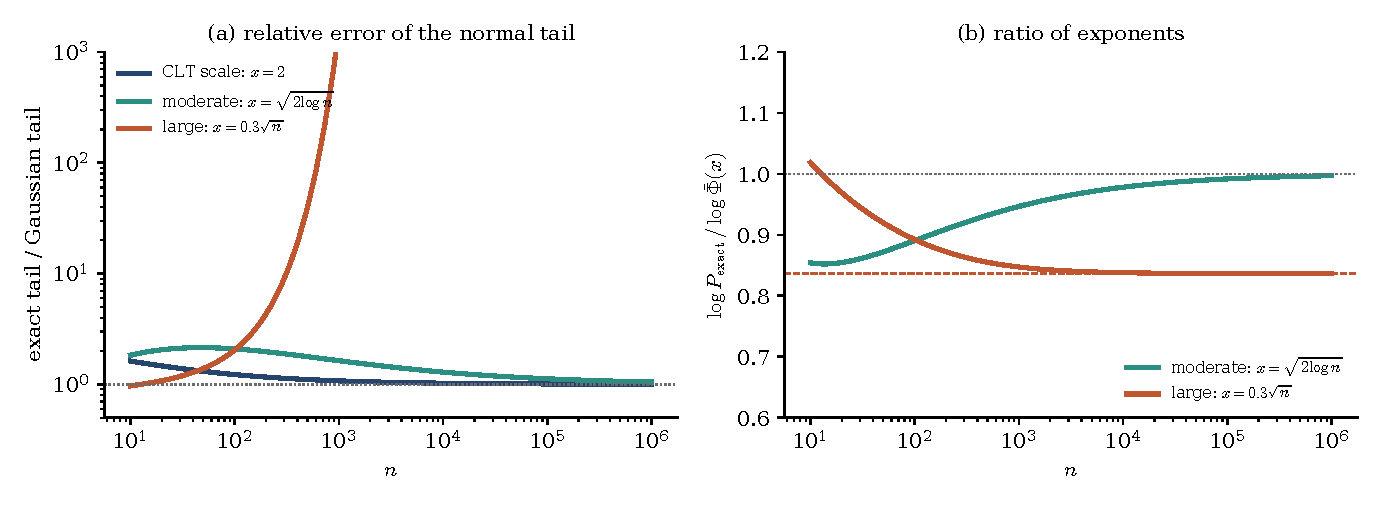
\includegraphics[width=\textwidth]{tst_three_scales}
\caption{Three scales for the tail of a sum of $n$ standard exponential variables, $x$ standard errors
above the mean. (a) Exact tail over Gaussian tail. (b) Exact log tail over Gaussian log tail; the
dashed line is Cram\'er's ratio $0.836$ at $\varepsilon=0.3$. The Gaussian exponent is correct on the
moderate scale and wrong on the large one.}
\label{fig:tst_scales}
\end{figure}

\subsection{The principle}\label{md:sec:principle}

\begin{theorem}[Moderate deviation principle for sums]\label{md:thm:mdp}
Let $X_1,X_2,\dots$ be i.i.d.\ with mean $\mu$, variance $\sigma^2>0$ and a finite moment generating
function near zero. Let $a_n\to\infty$ with $a_n/\sqrt n\to0$. Then for every Borel set
$A\subseteq\R$,
writing $Z_n=\sqrt n(\bar X_n-\mu)/a_n$,
\[
-\inf_{x\in A^\circ}\frac{x^2}{2\sigma^2}\ \le\ \liminf_{n}\frac1{a_n^2}\log\Pb(Z_n\in A)
\ \le\ \limsup_{n}\frac1{a_n^2}\log\Pb(Z_n\in A)\ \le\ -\inf_{x\in\bar A}\frac{x^2}{2\sigma^2}.
\]
\end{theorem}

The rate function $x^2/(2\sigma^2)$ is the second order Taylor expansion of Cram\'er's rate $I$ at
the mean, and that is the whole reason the principle holds: on the moderate scale the deviation is
small enough that only the curvature of $I$ at its minimum is seen, and that curvature is
$1/\sigma^2$. The proof is the G\"artner and Ellis argument with the cumulant generating function
expanded to second order (Appendix~\ref{app:ldtoolkit}). For a parametric model the same statement applied to the score
replaces $1/\sigma^2$ by the Fisher information.

For testing one needs more than the logarithmic statement. Rubin and Sethuraman (1965a) proved the
precise form at the testing scale $a_n=c\sqrt{\log n}$:
\begin{equation}\label{md:eq:rsprob}
\Pb\bigl(\sqrt n\,|\bar X_n-\mu|>c\,\sigma\sqrt{\log n}\bigr)\ \sim\ \frac{2}{c\sqrt{2\pi\log n}}\;n^{-c^2/2},
\end{equation}
which is the two sided Gaussian tail $2\bar\Phi(c\sqrt{\log n})$ to first order, under a
moment condition whose order grows with $c$ and in particular under Cram\'er's condition. The display
says that at $\sqrt{\log n}$ standard deviations the Gaussian tail is right not merely in exponent
but in relative error. That is the property a Bayes risk calculation consumes, and it is why their
paper on moderate deviation probabilities appeared in the same issue as their paper on Bayes risk
efficiency (Section~\ref{ch:evmdp}).

The posterior obeys the same principle. Eichelsbacher and Ganesh (2002a) show that, for a regular
model and a prior positive and continuous at the truth $\theta_0$, the posterior law of
$\sqrt n(\theta-\hat\theta_n)/a_n$ satisfies a moderate deviation principle with rate
$\tfrac12x^\top\Info(\theta_0)x$. So on the moderate scale the posterior is Gaussian in exponent,
with the Fisher information as precision, while on the large deviation scale its rate is the
divergence $\D{p_0}{p_\theta}$ of inverse Sanov (Theorem~\ref{thm:go}). The two rates agree to second
order because the Hessian of the divergence at the truth is the Fisher information.

\subsection{The MDP approach to a fixed sample test}\label{md:sec:fixed}

The approach has four steps, and each can be checked on the simplest case: $\bar X_n\sim
\N(\theta,1/n)$, null $\theta=0$, a prior density $\pi$ on the alternative with $\pi(0)=c_\pi>0$, and
prior odds $\pi_0/\pi_a$.

\emph{Step 1: write the Bayes rule as a threshold on evidence.} Under zero one loss the Bayes rule
rejects when the posterior odds of the alternative exceed one, that is when
$BF_{a0}=m_a(\bar x)/f(\bar x\mid0)>\pi_0/\pi_a$. This is the likelihood ratio of
Theorem~\ref{ev:thm:canonical}, so the representation layer is fixed.

\emph{Step 2: find the scale on which the threshold must sit.} The marginal under the alternative is
nearly flat near the null, $m_a(\bar x)\approx c_\pi$, while the null density is
$\sqrt{n/2\pi}\,e^{-t^2/2}$ with $t=\sqrt n\,\bar x$. The Bayes factor is therefore
$BF_{a0}\approx c_\pi\sqrt{2\pi/n}\,e^{t^2/2}$, and it crosses a constant only when $t^2/2$ has
caught up with $\tfrac12\log n$. A fixed $t$ gives $BF_{a0}\to0$, so the boundary cannot stay on the
central limit scale; a $t$ of order $\sqrt n$ is absurdly far out. The boundary is at
$t\asymp\sqrt{\log n}$, the moderate deviation scale.

\emph{Step 3: compute the errors with the MDP.} At $t_n=c\sqrt{\log n}$ the type I error is the
moderate deviation probability \eqref{md:eq:rsprob}, of order $n^{-c^2/2}/\sqrt{\log n}$, and the
prior weighted type II error is the prior mass of alternatives too close to the null to be detected,
of order $c\sqrt{\log n/n}$. Balancing the two gives $c^2=1$ to leading order, so both errors are
polynomially small and neither is negligible. Without the MDP Step 3 is impossible: the central limit
theorem does not control relative errors at $\sqrt{\log n}$ standard deviations, and the large
deviation exponent is the wrong exponent.

\emph{Step 4: read off the boundary.} Equating the Bayes factor to the prior odds gives
\[
t^2_{\mathrm{crit}}=\log n+\log(c_\pi^{-2})-\log(2\pi)+2\log(\pi_0/\pi_a)+o(1),
\]
which is Theorem~\ref{dv:thm:threshold} of Section~\ref{ch:deviations}. The leading term $\log n$ is
universal, coming from the $\sqrt n$ concentration of the likelihood against the $O(1)$ spread of the
prior; the constant carries the prior density at the null and the prior odds. Lindley's paradox,
the BIC penalty, and the comparison with a fixed level test all follow, and are worked out in
Section~\ref{ch:deviations}. The general form, for $k$ parameters and a prior times loss weight that
vanishes like $\|\theta\|^\lambda$, is Rubin and Sethuraman's theorem (Section~\ref{ch:evmdp}).

\subsection{The MDP approach to a sequential test}\label{ev:sec:stopping}

Now let the data arrive one at a time and stop when the evidence is strong enough. Let
$E_n=\prod_{t\le n}p_1(X_t)/p_0(X_t)$ be the likelihood ratio e-process. Under correct specification
$n^{-1}\log E_n\to\D{P_1}{P_0}$ almost surely; under misspecification with truth $P$ the limit is
$\D{P}{P_0}-\D{P}{P_1}$, which can be negative. Write $Y_t=\log\{p_1(X_t)/p_0(X_t)\}$ with
$\mu=\E_{P_1}[Y_t]=\D{P_1}{P_0}>0$, variance $\sigma^2$, and a Cram\'er condition; set
$S_t=\sum_{i\le t}Y_i$ and stop at $\tau_b=\inf\{t:S_t\ge\log b\}$.

\begin{theorem}[Moderate deviation stopping]\label{ev:thm:stopping}
Under these conditions:
\emph{(i)} $\Pb_{P_0}(\tau_b<\infty)\le1/b$;
\emph{(ii)} $\E_{P_1}[\tau_b]=(\log b)/\mu+O(1)$;
\emph{(iii)} $\bigl(\tau_b-(\log b)/\mu\bigr)\big/\sqrt{(\sigma^2/\mu^3)\log b}\Rightarrow\N(0,1)$ as
$b\to\infty$, so $\tau_b$ fluctuates on the scale $\sqrt{\log b}$.
Hence the expected sample size to reject at level $\alpha=1/b$ is
$\E_{P_1}[\tau_{1/\alpha}]=\log(1/\alpha)/\D{P_1}{P_0}+O(1)$.
\end{theorem}

\begin{proof}
(i) Under $P_0$ the process $E_t=e^{S_t}$ is a nonnegative martingale with $E_0=1$, and
$\{\tau_b<\infty\}=\{\sup_tE_t\ge b\}$, so Ville's inequality gives the bound.
(ii) Under $P_1$ the walk has positive drift, so $\tau_b<\infty$ almost surely and Wald's identity
gives $\mu\,\E_{P_1}[\tau_b]=\E_{P_1}[S_{\tau_b}]=\log b+\E_{P_1}[R_b]$, with overshoot
$R_b=S_{\tau_b}-\log b\ge0$. Lorden's inequality bounds $\E[R_b]\le\E[(Y_1^+)^2]/\mu$ uniformly in
$b$, which gives the $O(1)$ remainder.
(iii) The first passage time of a random walk with positive drift over a level $\ell$ satisfies a
central limit theorem with centering $\ell/\mu$ and variance $\sigma^2\ell/\mu^3$ (the renewal central
limit theorem); put $\ell=\log b$. Wald's second identity confirms the variance:
$\E[(S_{\tau_b}-\mu\tau_b)^2]=\sigma^2\E[\tau_b]$, and since $S_{\tau_b}=\log b+O(1)$ this is
$\mu^2\Var(\tau_b)+O(\sqrt{\log b})$.
\end{proof}

The theorem is a moderate deviation statement in the following precise sense. Part (iii) says the
stopping time is Gaussian on the scale $\sqrt{\log b}$, and the probability that it overshoots its
center by $x\sqrt{\log b}$ is at most $\exp\{-\mu^3x^2(1+o(1))/(2\sigma^2)\}$ for $x$ in
the moderate band, by Theorem~\ref{md:thm:mdp} applied to $S_t$ through $\{\tau_b>t\}\subseteq\{S_t<\log b\}$. The validity guarantee (i) is
polynomial in $b$, and the efficiency guarantee (ii) is logarithmic in $b$; the bridge between them
is the divergence $\mu$.

\paragraph{Checking the theorem.} Test $p=0.5$ against $p=0.65$ with Bernoulli data, so that
$\mu=\D{0.65}{0.5}=0.0457$ nats and $\sigma^2=0.0872$. Table~\ref{tab:tst_tau} reports $200{,}000$
simulated stopping times under $P_1$ for five thresholds. The mean exceeds $(\log b)/\mu$ by about
$2.5$ observations at every threshold, which is the constant overshoot of part (ii): Lorden's bound
caps it at $\E[(Y_1^+)^2]/\mu^2=21.4$ observations, and the actual value is far smaller. The standard
deviation tracks $\sqrt{(\sigma^2/\mu^3)\log b}$ to within three percent. Figure~\ref{fig:tst_seq}(b)
shows the distribution at $b=20$: it is visibly skewed, and the Gaussian of part (iii) is a poor fit,
while the inverse Gaussian law of the first passage time of Brownian motion with the same drift and
variance fits well. The Gaussian shape is an asymptotic statement in $\log b$, and $\log 20\approx3$
is not large; the mean and the variance, which is what a sample size calculation uses, are already
accurate.

\begin{table}[t]
\centering\small
\begin{tabular}{rrrrrr}
\toprule
$b$ & $(\log b)/\mu$ & mean of $\tau_b$ & mean minus $(\log b)/\mu$ & sd of $\tau_b$ & $\sqrt{(\sigma^2/\mu^3)\log b}$\\
\midrule
$10$ & $50.4$ & $53.0$ & $2.6$ & $47.2$ & $45.9$\\
$20$ & $65.6$ & $68.1$ & $2.6$ & $53.3$ & $52.3$\\
$50$ & $85.6$ & $88.1$ & $2.5$ & $60.7$ & $59.8$\\
$100$ & $100.8$ & $103.3$ & $2.5$ & $65.6$ & $64.9$\\
$200$ & $115.9$ & $118.4$ & $2.5$ & $70.2$ & $69.6$\\
\bottomrule
\end{tabular}
\caption{Stopping times of the likelihood ratio e-process, $\mathrm{Bern}(0.5)$ against
$\mathrm{Bern}(0.65)$, $200{,}000$ replications under the alternative. The excess over $(\log b)/\mu$
is a constant overshoot; the spread grows like $\sqrt{\log b}$.}
\label{tab:tst_tau}
\end{table}

\begin{figure}[H]
\centering
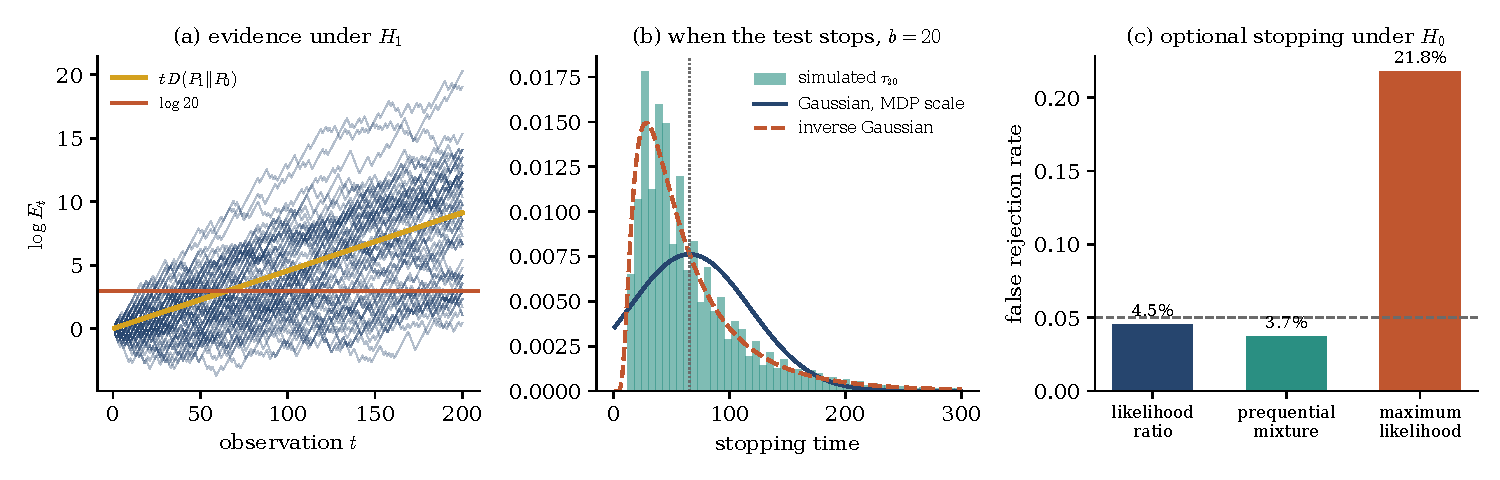
\includegraphics[width=\textwidth]{tst_sequential}
\caption{Sequential evidence for $\mathrm{Bern}(0.5)$ against $\mathrm{Bern}(0.65)$. (a) Sixty paths of
$\log E_t$ under the alternative, the drift line $t\,\D{P_1}{P_0}$, and the threshold $\log20$.
(b) The distribution of $\tau_{20}$ from $200{,}000$ replications, with the Gaussian limit of
Theorem~\ref{ev:thm:stopping}(iii) and the inverse Gaussian first passage law. (c) False rejection
rates under the null with continuous monitoring up to $T=500$, for three evidence processes
(Section~\ref{ch:testpractice}).}
\label{fig:tst_seq}
\end{figure}

\begin{corollary}[Finite sample detection tail]\label{md:cor:tail}
If the increments $Y_t$ take values in an interval of length $\rho$, then for every
$t\ge(\log b)/\mu$,
\[
\Pb_{P_1}(\tau_b>t)\le\exp\Bigl\{-\frac{2(\mu t-\log b)^2}{t\rho^2}\Bigr\}.
\]
\end{corollary}

\begin{proof}
$\{\tau_b>t\}\subseteq\{S_t<\log b\}=\{S_t-\mu t<-(\mu t-\log b)\}$, and Hoeffding's inequality bounds
the last probability.
\end{proof}

The bound is a guarantee, not an approximation. In the Bernoulli example $\rho=\log(1.3/0.7)=0.619$,
and at $b=20$ the bound gives $0.879$, $0.596$ and $0.373$ at $t=100,150,200$, against simulated
values $0.184$, $0.073$ and $0.031$. A Gaussian constant $\sigma^2$ in place of $\rho^2/4$ would be
sharper, and is valid when the increments are themselves Gaussian, as in the worked example of
Section~\ref{ch:evalues}, but it is not valid for skewed increments in general.

\paragraph{Misspecification.} Suppose the alternative is wrong: data come from $P$ with
$\delta=\D{P}{P_0}-\D{P}{P_1}<0$. The evidence then drifts toward the null even though the null is
false. How often does it still cross the threshold? The answer is again a Ville argument. Let
$\theta^\ast>0$ solve $\E_P[e^{\theta^\ast Y}]=1$, the Lundberg exponent of the walk. Then
$e^{\theta^\ast S_t}$ is a nonnegative $P$ martingale, and Ville's inequality gives
\begin{equation}\label{md:eq:lundberg}
\Pb_P(\tau_b<\infty)=\Pb_P\Bigl(\sup_te^{\theta^\ast S_t}\ge b^{\theta^\ast}\Bigr)\le b^{-\theta^\ast}.
\end{equation}
Take $P=\mathrm{Bern}(0.55)$, null $0.5$ and alternative $0.80$. The drift is $\delta=-0.154$ nats per
observation, and $\theta^\ast=0.691$. The bound \eqref{md:eq:lundberg} gives $0.126$, $0.041$ and
$0.0084$ at $b=20$, $100$ and $1000$; simulation with $100{,}000$ paths over $1500$ observations gives
$0.103$, $0.036$ and $0.0073$. So the bound is nearly tight, and the crossing probability is not
small: about one path in ten rejects the null at $b=20$, almost always early (median crossing time
$19$ observations), before the negative drift takes hold. Figure~\ref{fig:tst_misspec} shows
it. A bad choice of alternative makes the test weak, not silent, and mixing over alternatives, the
Bayesian mixture closure of Section~\ref{ch:evalues}, restores the growth rate.

\begin{figure}[H]
\centering
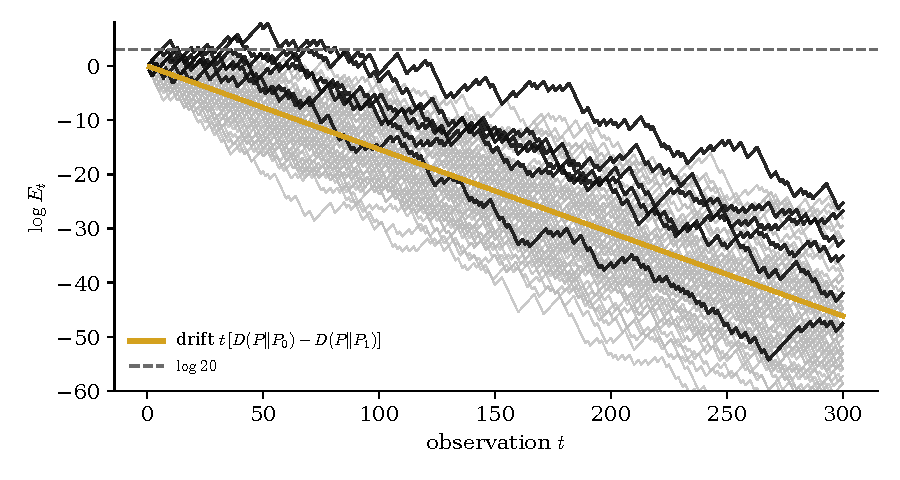
\includegraphics[width=0.75\textwidth]{tst_misspec}
\caption{Eighty paths of $\log E_t$ when the alternative $\mathrm{Bern}(0.8)$ is wrong and the data
are $\mathrm{Bern}(0.55)$. The drift is $-0.154$ nats per observation, but paths that cross
$\log20$, which reach the dashed line, do so early; about ten percent cross, close to the Lundberg
bound $20^{-0.691}=0.126$.}
\label{fig:tst_misspec}
\end{figure}

\paragraph{Validity alone does not give a rate.} The likelihood ratio detects at the rate
$(\log b)/\mu$ because its logarithm is a random walk with drift $\mu$. A process that is merely an
e-process need not grow at all. A null martingale frozen at a fixed time $T$ is a valid e-process
with $\lim_tt^{-1}\log E_t=0$, so its only guarantee is the polynomial $1/b$ of Ville, with no
detection rate behind it. Representation (the likelihood ratio) is what turns a validity certificate
into an efficient test, which is the point of Figure~\ref{fig:tst_layers}.

\paragraph{Summary.} The moderate deviation principle says that $\sqrt{\log n}$ standard deviations
out, the Gaussian exponent is right for any law with a moment generating function, and the Rubin and
Sethuraman refinement makes it right in relative error. Bayes tests put their boundaries
there, because a Bayes factor against a diffuse alternative balances the $\sqrt n$ concentration of
the likelihood against the $O(1)$ spread of the prior. In sequential form the same principle says
that the likelihood ratio test stops after $(\log b)/\D{P_1}{P_0}$ observations with $\sqrt{\log b}$
fluctuations, while Ville's inequality holds its false alarm rate at $1/b$.

\subsection*{Problems}
\begin{enumerate}[leftmargin=2.2em,itemsep=2pt]
\item Prove Theorem~\ref{md:thm:mdp} by expanding the cumulant generating function to second order
and applying the G\"artner and Ellis theorem with speed $a_n^2$.
\item For sums of standard exponentials, show that the ratio of exponents on the large deviation scale
$x=\varepsilon\sqrt n$ tends to $\{\varepsilon-\log(1+\varepsilon)\}/(\varepsilon^2/2)$, and evaluate it at
$\varepsilon=0.3$.
\item Show that the Bayes factor of Step 2 tends to zero for every fixed $t$ and to infinity for
every $t$ with $t^2-\log n\to\infty$, so the boundary must lie on the moderate scale.
\item Prove parts (i) and (ii) of Theorem~\ref{ev:thm:stopping}, and use Lorden's inequality to bound
the overshoot in the Bernoulli example.
\item Compute the Lundberg exponent $\theta^\ast$ for the misspecified Bernoulli example and verify
\eqref{md:eq:lundberg} by simulation.
\item Give an e-process whose logarithm grows sublinearly under every alternative, and explain which
layer of Figure~\ref{fig:tst_layers} it fails.
\end{enumerate}

\src{Bayes, E-values, and Testing (Polson, Sokolov and Zantedeschi, 2026a, arXiv:2602.04146), whose
Theorem~5.4 is stated here with an $O(1)$ remainder and whose finite sample and misspecification
bounds are replaced by the Hoeffding and Lundberg forms above after checking them by simulation; Rubin
and Sethuraman (1965a) on probabilities of moderate deviations; Eichelsbacher and Ganesh (2002a) on
moderate deviations of posteriors; Lorden (1970) on overshoot; Siegmund (1985) on sequential
analysis. All numbers in this section were computed for the book from the code in the book's code
archive.}


%====================================================================================================

\shorthead{The Three Deviation Regimes}
\section{The Three Deviation Regimes and the Bayesian Testing Threshold}\label{ch:deviations}

\noindent\textbf{Thesis.} Central-limit, moderate, and large deviations are three
scales, and Bayesian evidence lives on the middle one. Fixing the sample size, the
risk-optimal rejection boundary for a Bayes factor sits in the moderate-deviation
regime, a square-root logarithmic inflation above the local asymptotic normal scale.
The threshold's leading term $\log n$ is universal across regular models and priors;
its additive constants carry the local prior density, the Fisher information, and
the prior model odds. This one boundary places Jeffreys' testing threshold,
Lindley's paradox, the Bayesian information criterion penalty, and the
Chernoff--Stein error exponents on a common coordinate system. The fixed-sample
threshold here is the companion to the sequential stopping boundary of
Section~\ref{ch:evalues}, both governed by the polynomial tail decay at the
moderate-deviation scale.

\subsection{Testing framework and the three regimes}\label{dv:sec:regimes}

Test $H_0:\theta=\theta_0$ against $H_a:\theta\neq\theta_0$ from $X_1,\dots,X_n$
i.i.d.\ with density $f(\cdot\mid\theta)$, alternative prior $\pi$, and prior model
probabilities $\pi_0,\pi_a$. Write $\lambda_n=|\hat\theta-\theta_0|$ for the
parameter deviation and $t_n=\sqrt n\,\lambda_n/\sigma$ for the standardized
statistic, $\sigma^2=\Var_{\theta_0}(X_1)$. The scale of $\lambda_n$ fixes the tail
behavior and sorts the problem into three regimes. On the \emph{central-limit}
scale $\lambda_n=O(n^{-1/2})$, equivalently $t_n=O(1)$, tail probabilities are
$O(1)$ and do not decay. On the \emph{large-deviation} scale $\lambda_n=c$ fixed,
they decay exponentially, $\Prob(\bar X_n-\theta_0>c)=\exp\{-nI(c)+o(n)\}$ with
$I(c)=\sup_t\{tc-\psi(t)\}$ Cram\'er's rate function and $\psi$ the cumulant
generating function of $X_1-\theta_0$. Between them, on the \emph{moderate-deviation} scale
$\lambda_n=a\sqrt{(\log n)/n}$, the two-sided tail decays polynomially,
\[
\Prob_{\theta_0}\!\big(|\bar X_n-\theta_0|>\lambda_n\big)\sim
\frac{\sqrt2\,\sigma}{a\sqrt{\pi\log n}}\;n^{-a^2/(2\sigma^2)} .
\]
Fixed-$\alpha$ classical testing operates on the central-limit scale with a constant
critical value; simple-versus-simple Bayes risk is governed by the large-deviation
scale through the Chernoff exponent; the Bayes-rule threshold for a composite
alternative lies on the intermediate scale, where both likelihood concentration and
prior-mass allocation matter.

\subsection{Bayes risk and the moderate-deviation balance}\label{dv:sec:risk}

Write the null density $f(x\mid\theta_0)$, the Bayes mixture
$m(x)=\int f(x\mid\theta)\pi(d\theta)$, and $\log BF_{01}=\log f(x\mid\theta_0)-\log
m(x)$. The identity $m(\mathbf x)p(\theta\mid\mathbf x)=f(\mathbf x\mid\theta)\pi(\theta)$
gives two forms of the integrated Bayes risk under $0/1$ loss: a posterior-risk form
yielding the pointwise rule $\delta^\ast=\ind\{BF_{01}<\pi_a/\pi_0\}$, and a
prior-risk form $B_n=\pi_0\alpha_n+\pi_a\beta_n$ exposing how a threshold rule is
calibrated by moderate deviations of the test statistic. The Type~I term
$\alpha_n=\Prob_{\theta_0}(|t_n|>c)$ decays like $e^{-c^2/2}$ by Gaussian tail
asymptotics; the Type~II term integrates the failure-to-reject probability against
the prior, and for alternatives within an $n^{-1/2}$ neighborhood of the null the
posterior concentrates at rate $\sqrt n$, producing a factor $n^{-1/2}$. The two
rates balance, and the risk is minimized when $e^{-c^2/2}\asymp n^{-1/2}$,
that is when $c^2=\log n+O(1)$. A fixed threshold would leave Type~I error
undecayed; a threshold growing faster than $\sqrt{\log n}$ would let Type~II error
dominate. The logarithmic rate is the unique balancing point.

The tail approximations come from a uniform moderate-deviation lemma: under the
Cram\'er condition, with $z_n=\sqrt n\lambda_n/\sigma=(a/\sigma)\sqrt{\log n}$, the
Cram\'er moderate-deviation theorem plus Mills' ratio give the displayed polynomial
decay, uniformly for $a$ in compact subsets of $(0,\infty)$. A saddlepoint
refinement expresses the density of $\hat\theta$ with relative error $O(n^{-1})$ and
exponent $-nI(\hat\theta)$, bridging the large-deviation exponent and the
moderate-deviation prefactor.

\subsection{The risk-optimal threshold}\label{dv:sec:threshold}

\begin{theorem}[Risk-optimal Bayes-factor threshold]\label{dv:thm:threshold}
Let $\bar X_n\sim\N(\theta,\sigma^2/n)$ with $\sigma$ known, null $\theta_0=0$, and the alternative
prior $C^3$ near the null with $\pi(0)=c_\pi>0$ and at most polynomial growth. Then,
uniformly for $\bar x$ on the moderate-deviation band $|\bar x|=O(\sqrt{(\log n)/n})$,
\[
BF_{01}(\bar x)=\frac{\sqrt n}{\sigma\sqrt{2\pi}\,c_\pi}\,e^{-t^2/2}
\big(1+O(\sqrt{(\log n)/n})\big),\qquad t=\sqrt n\,\bar x/\sigma,
\]
and setting $BF_{01}=\pi_a/\pi_0$ gives
\[
t^2_{\mathrm{crit}}=\log n+\log(c_\pi^{-2})-\log(2\pi\sigma^2)
+2\log(\pi_0/\pi_a)+O(\sqrt{(\log n)/n}).
\]
\end{theorem}

The proof is a Laplace expansion of $m_a(\bar x)=\int f(\bar x\mid\theta)\pi(\theta)
\,d\theta$. Substituting $u=\sqrt n(\theta-\bar x)/\sigma$ and splitting the integral
into a good set $|u|\le M_n$ (any $M_n$ with $M_n/\sqrt{\log n}\to\infty$ and $M_n/\sqrt n\to0$) and its
complement, a uniform second-order Taylor expansion of $\pi$ about $\bar x$ on the good set, valid
because the argument stays in a shrinking neighborhood of the null on the
moderate-deviation band, has its first-order term vanish by symmetry, while the
polynomial-growth bound kills the bad set faster than any power of $n$. What remains
is $\pi(\bar x)+O(1/n)$, and $\pi(\bar x)=c_\pi+\pi'(0)\bar x+O(\bar x^2)$ with
$|\bar x|=O(\sqrt{(\log n)/n})$ on the band, so the result is
$m_a(\bar x)=c_\pi(1+O(\sqrt{(\log n)/n}))$; dividing the null likelihood by this
gives the displayed Bayes factor, and equating to the prior odds gives the
threshold. The rule is Bayes-risk-optimal because it is the Bayes decision boundary
under $0/1$ loss.

Three features stand out. The leading term $t^2_{\mathrm{crit}}\sim\log n$ is
\emph{universal}: it is the balance between the $\sqrt n$ Fisher-information
prefactor and the Gaussian tail, and depends on neither the prior family nor the
model. The additive constant is \emph{prior-sensitive}, carrying $\log(c_\pi^{-2})$:
a flatter local prior raises the bar. And the remainder is deterministic and
vanishing on the band, so the constants are identified.

\begin{corollary}[Cauchy prior; sample-size adaptivity]\label{dv:cor:cauchy}
For $\theta\sim C(0,\sigma)$, $c_\pi=1/(\pi\sigma)$ and, at equal prior odds,
$t_{\mathrm{crit}}=\sqrt{\log(\pi n/2)}\,(1+o(1))$. The cutoff falls below $1.96$ for
small $n$ and rises above it for large $n$; its leading term is $1.44$ at $n=5$ (where the exact cutoff is $1.72$), $2.71$ at $n=1000$,
and $3.46$ at $n=10^5$.
\end{corollary}

This is Lindley's paradox, read as a scale mismatch and not a pathology. A fixed
level holds $t$ at $z_{1-\alpha/2}$ while the risk-optimal boundary drifts out as
$\sqrt{\log n}$; past a crossover the Bayesian rejection region lies inside the
classical rejection region, so a $p$-value of $0.05$ can correspond to a Bayes
factor favoring $H_0$. The same $\log n$ bookkeeping is the BIC penalty
$(d/2)\log n$, the identical Laplace prefactor applied to the log marginal
likelihood; the threshold governs evidence accumulation and the penalty governs
model complexity, but they are one polynomial correction seen at the two ends of the
same integral.

\subsection{Extensions}\label{dv:sec:extensions}

\paragraph{Exponential families.}
The scaling survives beyond the Gaussian model through local asymptotic normality.
For a one-parameter exponential family with Fisher information $\Info(\theta_0)$ and
standardized score $S_n$, completing the square in the LAN expansion of the marginal
likelihood gives
$BF_{01}=\{\sqrt{n\Info(\theta_0)}/(\sqrt{2\pi}\,c_\pi)\}\exp(-S_n^2/2)(1+O((\log
n)^{3/2}/\sqrt n))$ and the threshold
$S_n^2=\log n+\log(c_\pi^{-2})+\log\Info(\theta_0)-\log(2\pi)+2\log(\pi_0/\pi_a)
+O((\log n)^{3/2}/\sqrt n)$, the Gaussian result with $\sigma^{-2}$ replaced by
$\Info(\theta_0)$.

\paragraph{Separated alternatives.}
For simple-versus-simple testing the Bayes risk vanishes at the exponential
Chernoff rate $\exp(-nD_C)$ with $D_C=-\min_{0\le s\le1}\log\int f_{\theta_0}^{1-s}
f_{\theta_1}^{s}$; the Efron--Truax (1968) refinement supplies the polynomial prefactor
$K/\sqrt n$. This is the fixed-separation lineage, exponential in $n$. The
moderate-deviation boundary is the local, composite-alternative refinement: once the
alternative is integrated against a prior and allowed to shrink toward the null, the
mixture structure makes the polynomial prefactor first-order relevant, and it is
this prefactor that produces the logarithmic correction.

\paragraph{The Rubin--Sethuraman calculus and sparsity.} Section~\ref{ch:evmdp} develops this in full;
here is the summary.
The systematic moderate-deviation analysis of Bayes risk is due to Rubin and
Sethuraman: with a local prior-times-loss weight $g(\theta)=\gamma(\theta)\|\theta\|
^\lambda h(\theta/\|\theta\|)$, the boundary is $\|\hat\theta\|=\sqrt{(\log n)/n}\,
(\lambda+d+o(1))^{1/2}$ for $\theta\in\R^d$ with identity Fisher information, and the risk splits into a $\sqrt{\log n}$-scaled term and a
polynomial term. The scaling has a sparse counterpart: under the two-groups model
with sparsity $p\to0$, the horseshoe rule achieves the Bayes oracle risk up to a multiplicative constant when the
effective threshold grows like $\sqrt{\log(1/p)}$, the sparse analogue of the
Rubin--Sethuraman boundary with $1/p$ replacing $n$, as developed in
Section~\ref{ch:hsmdp}. A prior of horseshoe type, whose density has a logarithmic pole
$\pi(\theta)\asymp\log(1/|\theta-\theta_0|)$ at the null, shifts the boundary to
$t^2_{\mathrm{crit}}=\log n-2\log\log n+O(1)$, because $m_a\asymp\log n$ on the band.

\subsection{Comparison of calibrations}\label{dv:sec:comparison}

Three calibrations of the same test differ only in how the threshold scales with
$n$. The risk-optimal rule grows, $t_{\mathrm{crit}}=\sqrt{\log n+O(1)}$; the
Neyman\index{Neyman--Pearson}--Pearson fixed-$\alpha$ rule is constant, $t_{\mathrm{crit}}=z_{1-\alpha/2}$;
and the fixed-sample e-value (safe-testing) rule is constant in $n$,
$t_{\mathrm{crit}}=\sqrt{2\log(1/\alpha)}$, since it thresholds at $1/\alpha$ the
likelihood-ratio e-value against the alternative $\theta=\sigma\sqrt{2\log(1/\alpha)/n}$,
tuned to the sample size, and controls error at that $n$ by Markov's inequality
(Section~\ref{ch:evalues}). The ratio of the e-value threshold to the risk-optimal one tends to $0$ as $n\to\infty$: the
e-value threshold does not grow with sample size. No constant boundary controls error
uniformly over stopping times, since by the law of the iterated logarithm $t_n$
exceeds any constant infinitely often under $H_0$; the normal mixture e-process, the
Bayes factor against $\theta\sim\N(0,\tau^2)$, is anytime valid by Ville's inequality and
crosses $1/\alpha$ at $t_n^2=\log(1+n\tau^2/\sigma^2)+2\log(1/\alpha)+o(1)$, on the
moderate-deviation scale of the risk-optimal rule. Under integrated Bayes risk with
fixed prior weights and non-adaptive thresholds, only the risk-optimal calibration of the three
operates on the moderate-deviation scale, and the divergence between it and the
fixed-$\alpha$ value is the mechanism of Lindley's paradox. The comparison is
algebraic, not normative: risk minimization, Type~I control, and fixed-sample e-value validity
are distinct goals, and the scaling differences reflect them.

Collectively these strands, Jeffreys' threshold, the Rubin--Sethuraman calculus,
the Laplace/BIC prefactor, and the Chernoff--Stein exponents, converge on the
moderate-deviation scale as the unifying lens, and the three forms
$\lambda_n\asymp\sqrt{(\log n)/n}$, $t_n\asymp\sqrt{\log n}$, $t_n^2=\log n+O(1)$
are the coordinate system on which they are simultaneously situated. The same
calibration principle governs goodness-of-fit tests, where the $\sqrt{\log n}$
inflation arises for the Kolmogorov--Smirnov and $\chi^2$ statistics without any
Bayes-factor or likelihood-ratio structure, through the shared Sanov rate of the
test statistic.


\subsection{The threshold in numbers}\label{dv:sec:numbers}

The risk-optimal cutoff grows with the sample size while the classical one does not.
Under a Cauchy prior at equal prior odds, $t_{\mathrm{crit}}=\sqrt{\log(\pi n/2)}$;
the table contrasts it with the fixed classical value $1.96$ and shows the two-sided
Bayes-factor evidence $BF_{01}=\sqrt{\pi n/2}\,e^{-t^2/2}$ implied at $t=1.96$, both to the leading order of Theorem~\ref{dv:thm:threshold}.

\begin{table}[h]\centering
\begin{tabular}{@{}rccc@{}}
\toprule
$n$ & $t_{\mathrm{crit}}=\sqrt{\log(\pi n/2)}$ & classical $z$ & $BF_{01}$ at $t=1.96$ \\
\midrule
$5$ & $1.44$ & $1.96$ & $0.41$ \\
$50$ & $2.09$ & $1.96$ & $1.30$ \\
$100$ & $2.25$ & $1.96$ & $1.84$ \\
$1{,}000$ & $2.71$ & $1.96$ & $5.8$ \\
$10{,}000$ & $3.11$ & $1.96$ & $18.4$ \\
$100{,}000$ & $3.46$ & $1.96$ & $58.1$ \\
\bottomrule
\end{tabular}
\caption{The risk-optimal Bayes threshold rises like $\sqrt{\log n}$ while the
classical cutoff is flat. Past $n\approx30$ (to leading order) the observation $t=1.96$ that rejects at
level $0.05$ yields a Bayes factor favoring $H_0$, Lindley's paradox.}\label{dv:tab:thr}
\end{table}

\noindent The crossover near $n\approx30$ is where the growing Bayesian boundary
overtakes the fixed classical one; beyond it the two calibrations disagree by an
amount that widens without bound, and the disagreement is the $\sqrt{\log n}$
inflation of the moderate-deviation scale.
Exact integration of the Cauchy marginal gives $BF_{01}=0.70$, $1.42$ and $1.92$ in the first three rows, the tabulated values from $n=1000$ on, and a crossover near $n\approx20$; the table keeps the leading order, under which the cutoff reaches $1.96$ where $BF_{01}$ reaches one.





\subsection*{Worked example: a genome-wide threshold}
This example puts numbers on the moderate-deviation threshold at the scale of a real screen.

Fix $n=10^6$ (a genome-wide screen). The risk-optimal two-sided threshold under a unit-information prior and equal prior odds is $t_{\mathrm{crit}}=\sqrt{\log n}\approx\sqrt{13.82}\approx3.72$, corresponding to a per-test two-sided $p$-value of about $2\times10^{-4}$. The Bonferroni level for $m=10^6$ tests at family-wise error $0.05$ is $5\times10^{-8}$, i.e.\ $t\approx5.45$; the accepted genome-wide significance line $5\times10^{-8}$ is this Bonferroni boundary, which grows like $\sqrt{2\log m}$ to leading order ($\sqrt{2\log10^6}\approx5.26$). With $m=n$, as here, the two agree in growing like $\sqrt{\log m}$; the constant differs because at equal prior odds the single test pays only the Occam factor $(1+n)^{-1/2}$ of its unit-information prior, whereas Bonferroni pays the multiplicity $m$: to leading order both are the threshold $\sqrt{2\log b}$ of Section~\ref{ch:evmdp}, with $b=\sqrt n$ and $b=m$.

At equal prior odds the risk-optimal threshold sits well below the Bonferroni threshold, $3.72$ against $5.45$, a factor of about $4000$ in $p$-value; the risk-optimal one is derived from a loss rather than decreed, and it moves with the sample size like $\sqrt{\log n}$ instead of staying fixed. With prior odds $m$ against each association, the calibration of Section~\ref{ch:risk}, the term $2\log(\pi_0/\pi_a)$ of Theorem~\ref{dv:thm:threshold} adds $2\log m$ to $t^2_{\mathrm{crit}}$ and gives the genome-wide threshold $\{\log(m^2n)\}^{1/2}\approx6.44$ (two-sided $p\approx1.2\times10^{-10}$), above the Bonferroni line: once the multiplicity enters through the prior odds, the risk-optimal threshold is the stricter of the two.

\paragraph{Summary.}
The three deviation regimes, central-limit, moderate, large, are three scales, and Bayesian testing lives on the moderate one. The risk-optimal Bayes-factor threshold is $t^2_{\mathrm{crit}}=\log n+O(1)$, universal in its leading term and prior-sensitive in its constant. The same $\sqrt{\log}$ scale governs sparse recovery, bandits, and goodness-of-fit.

\subsection*{Problems}
\begin{enumerate}[leftmargin=2.2em,itemsep=2pt]
\item Derive the polynomial moderate-deviation tail $\Prob(|\bar X_n|>a\sqrt{(\log n)/n})\sim c\,(\log n)^{-1/2}n^{-a^2/(2\sigma^2)}$.
\item Prove the risk-optimal threshold theorem by a Laplace expansion of the marginal likelihood on the moderate-deviation band.
\item Show the exponential-family extension via local asymptotic normality, replacing $\sigma^{-2}$ by the Fisher information.
\item Locate the crossover sample size where the Bayesian boundary overtakes the fixed classical cutoff.
\item Compare the risk-optimal, fixed-$\alpha$, and fixed-sample e-value calibrations and explain why only the first grows with $n$.
\end{enumerate}

\src{A New Look at Bayesian Testing (Datta, Polson, Sokolov and Zantedeschi, 2026,
arXiv:2602.11132); Bayes Risk for Goodness of Fit Tests (Polson, Sokolov and
Zantedeschi, 2026b, arXiv:2602.15297); the moderate-deviation calculus of Rubin and
Sethuraman (1965a, 1965b).}


%====================================================================================================

\section{Rubin and Sethuraman: Bayes Risk and Testing Regions}\label{ch:evmdp}\index{Rubin Sethuraman balance}\index{Bayes risk efficiency}\index{testing region}

\noindent\textbf{Thesis.} In 1965 Herman Rubin and Jayaram Sethuraman asked a simple question:
if tests are judged by their Bayes risk rather than by a fixed level, where should the boundary go
and how should two tests be compared? Their answer has three parts. The boundary sits at
$\sqrt{(k+\lambda)\log n}$ standard errors, where $k$ is the dimension and $\lambda$ the order at
which prior times loss vanishes at the null. The minimal risk falls like $(\log n/n)^{(k+\lambda)/2}$,
dominated by missed signals near the null. And because every quantity is evaluated at a moderate
deviation, two tests compare through their Fisher informations alone, so Bayes risk efficiency agrees
with Pitman efficiency. This section derives each part, checks it numerically, and connects it to the
e-value and sequential calculus of the chapter.

\subsection{The question and the setting}\label{rs:sec:setting}

A fixed level test spends its type I error at a rate chosen in advance, and judges tests by power
at a fixed alternative or along a sequence of alternatives shrinking at rate $n^{-1/2}$. Rubin and
Sethuraman replaced both choices by a single prior weighted risk. Let $\hat\theta_n\in\R^k$ be
asymptotically $\N(\theta,I_k/n)$, which after a change of coordinates by the square root of the
Fisher information is the general regular case, and test $H_0:\theta=0$. Put prior mass $\pi_0$ on the
null with loss $L_{10}$ for a false rejection, and write $a_0=\pi_0L_{10}$. On the alternative put a
prior density $\pi_a(\theta)$ and a loss $\ell(\theta)$ for a false acceptance, and combine them into
the weight
\[
g(\theta)=\pi_a(\theta)\,\ell(\theta)\ \sim\ \gamma_0\,\|\theta\|^\lambda\,h(\theta/\|\theta\|)\qquad(\theta\to0),
\]
with $\gamma_0>0$, $\lambda\ge0$ and $h$ a positive continuous function on the unit sphere. The case
$\lambda=0$ is a prior positive at the null with constant loss; $\lambda=2$ is squared error loss
for accepting, which makes small departures cheap to miss. The Bayes risk of a test $\delta$ with
rejection region $\mathcal R$ is
\begin{equation}\label{rs:eq:risk}
B_n(\delta)=a_0\,\Pb_0(\hat\theta_n\in\mathcal R)+\int g(\theta)\,\Pb_\theta(\hat\theta_n\notin\mathcal R)\,d\theta .
\end{equation}
The first term is the prior weighted false alarm cost and the second the prior weighted missed signal
cost. Nothing in \eqref{rs:eq:risk} mentions a level.

\subsection{Step one: the Bayes rule}\label{rs:sec:rule}

Minimizing \eqref{rs:eq:risk} pointwise in the data, as in the proof of
Theorem~\ref{ev:thm:canonical}, gives the rule: reject when the weighted alternative density exceeds
the weighted null density,
\begin{equation}\label{rs:eq:rule}
\int g(\theta)\,f_n(\hat\theta\mid\theta)\,d\theta\ >\ a_0\,f_n(\hat\theta\mid0),
\qquad f_n(\hat\theta\mid\theta)=\Bigl(\frac n{2\pi}\Bigr)^{k/2}e^{-n\|\hat\theta-\theta\|^2/2}.
\end{equation}
This is a likelihood ratio rule with the prior odds and losses supplying the constant, the
representation layer of Figure~\ref{fig:tst_layers}. The work is in locating its boundary.

\subsection{Step two: where the boundary falls}\label{rs:sec:boundary}

\begin{theorem}[Rubin and Sethuraman boundary]\label{rs:thm:boundary}
Under the setting above, the Bayes rule \eqref{rs:eq:rule} rejects, for $\hat\theta$ in the moderate
band $\|\hat\theta\|=O(\sqrt{\log n/n})$, exactly when
\begin{multline*}
n\|\hat\theta\|^2\ >\ (k+\lambda)\log n\;-\;\lambda\log\bigl(n\|\hat\theta\|^2\bigr)\;-\;k\log(2\pi)\\
\;+\;2\log\frac{a_0}{\gamma_0h(u)}\;+\;o(1),\qquad u=\hat\theta/\|\hat\theta\|.
\end{multline*}
In particular the boundary is the sphere $\|\hat\theta\|=\sqrt{(k+\lambda+o(1))\log n/n}$.
\end{theorem}

\begin{proof}
The kernel $f_n(\hat\theta\mid\cdot)$ has width $n^{-1/2}$, while on the band $\|\hat\theta\|$ is of
order $\sqrt{\log n/n}$, larger by a factor $\sqrt{\log n}$. Across a window of width $n^{-1/2}$
around $\hat\theta$ the weight $g$ therefore changes by a relative amount $O(1/\sqrt{\log n})$, and a
Laplace argument gives $\int g(\theta)f_n(\hat\theta\mid\theta)\,d\theta=g(\hat\theta)(1+o(1))=
\gamma_0\|\hat\theta\|^\lambda h(u)(1+o(1))$. The right side of \eqref{rs:eq:rule} is
$a_0(n/2\pi)^{k/2}e^{-n\|\hat\theta\|^2/2}$. Take logarithms, write $\|\hat\theta\|^\lambda=
n^{-\lambda/2}(n\|\hat\theta\|^2)^{\lambda/2}$, and collect terms.
\end{proof}

Read the formula term by term. The $k\log n$ is the price of locating a $k$ dimensional parameter to
precision $n^{-1/2}$, the same term that becomes the BIC penalty $\tfrac k2\log n$ on the log scale.
The $\lambda\log n$ is the reward for cheap near misses: when missing a small effect costs little,
the test can afford to wait for stronger evidence. The $\log\log n$ correction and the constant carry
the local shape of prior and loss. Only the leading term is universal, and the boundary sits at
$\sqrt{(k+\lambda)\log n}$ standard errors, which is the moderate deviation scale of
Section~\ref{ch:mdptest}.

\paragraph{How good is the formula?} Table~\ref{tab:rs_boundary} solves \eqref{rs:eq:rule} exactly by
quadrature for $g(\theta)=\|\theta\|^\lambda e^{-\|\theta\|^2/2}$ and $a_0=1$, so $\gamma_0=1$ and
$h\equiv1$. The leading term $(k+\lambda)\log n$ overstates the boundary by a margin that does not
shrink, because the $\log\log n$ and constant terms are of the same order as the gap; the full
formula of Theorem~\ref{rs:thm:boundary}, solved as a fixed point in $n\|\hat\theta\|^2$, matches the
exact boundary to within $0.11$ in every case. The ratio of exact to leading order radius is $0.86$ at
$n=10^3$ and $0.93$ at $n=10^6$ for $\lambda=0$: the leading term is right, but it is approached at
the slow rate $1/\log n$, and the constant matters at every sample size a statistician will see.

\begin{table}[t]
\centering\small
\begin{tabular}{ccrrrr}
\toprule
$k$ & $\lambda$ & $n$ & exact $n\|\hat\theta\|^2$ & leading $(k+\lambda)\log n$ & Theorem~\ref{rs:thm:boundary}\\
\midrule
$1$ & $0$ & $10^3$ & $5.08$ & $6.91$ & $5.07$\\
$1$ & $0$ & $10^6$ & $11.98$ & $13.82$ & $11.98$\\
$1$ & $2$ & $10^3$ & $13.55$ & $20.72$ & $13.66$\\
$1$ & $2$ & $10^6$ & $32.58$ & $41.45$ & $32.64$\\
$2$ & $0$ & $10^3$ & $10.15$ & $13.82$ & $10.14$\\
$2$ & $0$ & $10^6$ & $23.96$ & $27.63$ & $23.96$\\
$3$ & $0$ & $10^3$ & $15.23$ & $20.72$ & $15.21$\\
$3$ & $0$ & $10^6$ & $35.93$ & $41.45$ & $35.93$\\
\bottomrule
\end{tabular}
\caption{The Bayes boundary of \eqref{rs:eq:rule}, solved exactly by quadrature, against the leading
term and the full expansion of Theorem~\ref{rs:thm:boundary}, for
$g(\theta)=\|\theta\|^\lambda e^{-\|\theta\|^2/2}$ and $a_0=1$.}
\label{tab:rs_boundary}
\end{table}

\subsection{Step three: the size of the risk}\label{rs:sec:riskorder}

Insert the boundary into \eqref{rs:eq:risk}. The missed signal term is, to leading order, the weight
$g$ integrated over the ball of undetectable alternatives, $\|\theta\|<r_n$ with
$r_n^2=(k+\lambda)\log n/n$, because by Theorem~\ref{rs:thm:boundary} the rule accepts inside a radius $r_n(1+o(1))$, uniformly in direction, and $\Pb_\theta(\hat\theta_n\notin\mathcal R)$ falls from near one to near zero across a shell of width $O(n^{-1/2})=o(r_n)$:
\[
\int_{\|\theta\|<r_n}g(\theta)\,d\theta\ \sim\ c_g\,r_n^{k+\lambda}
=c_g\Bigl(\frac{(k+\lambda)\log n}{n}\Bigr)^{(k+\lambda)/2},
\]
where $c_g=\gamma_0(k+\lambda)^{-1}\int_{\|u\|=1}h(u)\,d\sigma(u)$ and $\sigma$ is the surface measure on the unit sphere. The false alarm term is $a_0$ times a chi squared tail at $(k+\lambda)\log n$, which by the
boundary equation is smaller than the missed signal term by a factor of order $1/\log n$. So:

\begin{theorem}[Order of the minimal Bayes risk]\label{rs:thm:risk}
Under the setting above the minimal Bayes risk satisfies
$B_n^\ast\sim c_g\bigl((k+\lambda)\log n/n\bigr)^{(k+\lambda)/2}$, with $c_g$ as above, and the ratio of its false alarm part to its missed signal
part is of order $1/\log n$.
\end{theorem}

Two lessons follow. The risk falls polynomially, not exponentially, which is the signature of a
moderate deviation problem: a large deviation problem would have exponentially small risk, a central
limit problem risk bounded away from zero. And at the optimum almost all the risk is missed signals
close to the null. The test is not failing; those alternatives are indistinguishable from
the null at sample size $n$, and the boundary is placed so that the cost of chasing them with false
alarms just matches the cost of missing them.

Take $k=1$, $\lambda=0$, $a_0=1$ and $g$ the standard normal density, so $\gamma_0=\phi(0)$ and the
constant in Theorem~\ref{rs:thm:boundary} vanishes: the boundary is $t^2=\log n$. Minimizing
\eqref{rs:eq:risk} numerically over the threshold gives an optimal $t^2$ of $6.916$ at $n=10^3$ and
$13.816$ at $n=10^6$, against $\log n=6.908$ and $13.816$. The missed signal term is $0.0662$ and
$0.00297$, against the prediction $2\phi(0)\sqrt{\log n/n}=0.798\sqrt{\log n/n}$, which gives $0.0663$
and $0.00297$; the ratio of false alarm to missed signal is $0.129$ and $0.068$, against
$1/\log n=0.145$ and $0.072$. Figure~\ref{fig:tst_rs}(b) shows the two parts across five decades of
$n$.

\subsection{Step four: why this is a moderate deviation calculation}\label{rs:sec:whymdp}

Every probability in Steps two and three is evaluated at $\sqrt{\log n}$ standard errors. In the
Gaussian model that is exact algebra. For a real statistic, a sample mean of non Gaussian data, a
rank statistic, a likelihood ratio in a non Gaussian model, the calculation needs the tail
probabilities of the statistic at that distance, in relative error, uniformly over the alternatives
in the band. The central limit theorem does not supply them, because its error is additive and
$n^{-c^2/2}$ is no larger than that error, of order $n^{-1/2}$, once $c\ge1$; Cram\'er's large deviation theorem does not supply them
either, because its exponent is for fixed distances. The moderate deviation probabilities
\eqref{md:eq:rsprob}, which Rubin and Sethuraman proved for this purpose, are what is needed,
and they say that at this distance the statistic behaves like its Gaussian approximation. That is
the content of the phrase ``the MDP approach to testing'': compute the Bayes risk as if the statistic
were Gaussian with its Fisher information, and justify the computation by the moderate deviation
principle on the band where the boundary lives.

\subsection{Step five: comparing tests by Bayes risk}\label{rs:sec:efficiency}

Let $N_T(r)$ be the smallest sample size at which a test based on the statistic $T$, with its best
threshold, achieves Bayes risk $r$. The Bayes risk efficiency of $T$ relative to $T'$ is
$\lim_{r\to0}N_{T'}(r)/N_T(r)$.

\begin{proposition}[Bayes risk efficiency is a ratio of informations]\label{rs:prop:eff}
Suppose that, uniformly for $\theta$ in the moderate band, $T_n$ is asymptotically
$\N(\kappa\sqrt n\,\theta,1)$ and satisfies the moderate deviation tail \eqref{md:eq:rsprob}, and
likewise $T'_n$ with $\kappa'$. Then the Bayes risk efficiency of $T$ relative to $T'$ is
$\kappa^2/\kappa'^2$, the Pitman asymptotic relative efficiency.
\end{proposition}

\begin{proof}[Sketch]
On the band the risk \eqref{rs:eq:risk} of the best test based on $T_n$ depends on the data only
through tail probabilities of $T_n$ at moderate deviations, and by assumption these equal those of a
Gaussian statistic with information $\kappa^2n$ up to factors $1+o(1)$. Hence $B^\ast_{T}(n)=
B^\ast_{\mathrm{Gauss}}(\kappa^2n)(1+o(1))$. By Theorem~\ref{rs:thm:risk}, $B^\ast_{\mathrm{Gauss}}(m)\sim c_g\bigl((k+\lambda)\log m/m\bigr)^{(k+\lambda)/2}$ is regularly varying
with negative index, so equal risks force $\kappa^2N_T\sim\kappa'^2N_{T'}$.
\end{proof}

This places the Rubin and Sethuraman notion between the two classical efficiencies. Pitman
efficiency compares tests at a fixed level along alternatives shrinking like $n^{-1/2}$, on the
central limit scale. Bahadur efficiency compares exponential rates at fixed alternatives, on the
large deviation scale, and depends on the whole law of the data. Bayes risk efficiency compares on
the moderate scale, and the moderate deviation principle collapses it onto the Fisher information,
so for regular statistics it agrees with Pitman. Kallenberg's intermediate efficiency (1983) is the
same idea without a prior.

\paragraph{The sign test against the mean.} For normal data the sign test has efficacy
$\kappa=2\phi(0)=\sqrt{2/\pi}$ relative to the mean, so the proposition predicts a sample size ratio
of $\pi/2=1.571$. Figure~\ref{fig:tst_rs}(c) computes it exactly: the sign test uses the binomial law
of the number of positive observations, the mean test the normal law, each with its best threshold,
under a standard normal weight on the alternative. To match the Bayes risk of the sign test with
$50$, $100$, $200$, $400$, $800$ and $1600$ observations, the mean test needs $31.2$, $62.7$, $126.4$,
$253.5$, $507.9$ and $1017.1$, ratios of $1.604$, $1.596$, $1.583$, $1.578$, $1.575$ and $1.573$. The
ratio falls steadily to $\pi/2$, at the slow logarithmic rate that the regularly varying risk
predicts.

\begin{figure}[H]
\centering
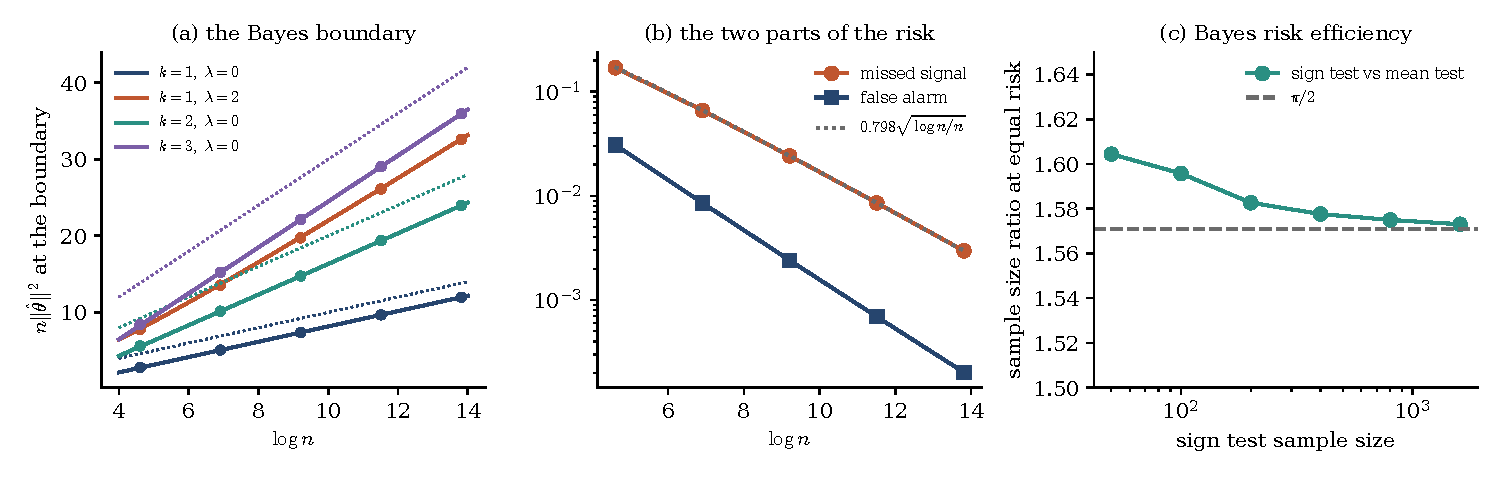
\includegraphics[width=\textwidth]{tst_rubin_sethuraman}
\caption{Rubin and Sethuraman checked numerically. (a) The exact Bayes boundary $n\|\hat\theta\|^2$
(points), the leading term $(k+\lambda)\log n$ (dotted) and the full expansion of
Theorem~\ref{rs:thm:boundary} (solid). (b) The false alarm and missed signal parts of the minimal
Bayes risk for $k=1$, $\lambda=0$, with the prediction $0.798\sqrt{\log n/n}$. (c) Sample size of the
mean test needed to match the Bayes risk of the sign test, as a ratio, converging to $\pi/2$.}
\label{fig:tst_rs}
\end{figure}

\subsection{The balance in its simplest form}\label{ev2:sec:rs}

The whole argument has a two point skeleton that is worth seeing in closed form. With prior
probabilities $\pi_0,\pi_1$ and a threshold $c$ the integrated risk is
\[
B(c)=\pi_0\,\alpha(c)+\pi_1\,\beta(c),
\]
the false alarm and missed signal probabilities weighted by the prior. The two terms move in opposite
directions in $c$, so the optimum is where their derivatives cancel: the testing region is the set on
which the posterior expected loss of rejecting is below that of accepting, and its boundary is where
the two weighted error densities are equal.

Take $T\sim\N(0,1)$ under the null and $T\sim\N(\Delta,1)$ under the alternative, with $\Delta>0$ and prior odds
$\pi_0/\pi_1=b$, where $b$ counts the hypotheses the procedure must guard against. Setting
$B'(c)=0$ gives, with $\phi$ the standard normal density, $b\,\phi(c)=\phi(c-\Delta)$, hence
\begin{equation}\label{ev2:eq:cstar}
c^*=\frac{\log b}{\Delta}+\frac{\Delta}{2}.
\end{equation}
If the signal is strong relative to the multiplicity, $\log b=o(\Delta^2)$, the first term is
negligible and $c^*\approx\Delta/2$: the threshold sits halfway and the prior enters only at second
order. If instead the problem is at the detectability boundary, $\Delta=\sqrt{2\log b}$, the two terms
are equal and
\[
c^*=\sqrt{2\log b},
\]
the canonical moderate deviation threshold. The multiple comparison scale is not imposed; it is the
output of a risk calculation, and the same number appears in Bonferroni style multiplicity, in the
universal threshold of wavelet shrinkage, and in the sparse prior thresholds of
Section~\ref{ch:hsmdp}, with $b$ respectively the number of tests, the number of coefficients, and the prior odds $n/p_0$ against a coordinate carrying signal. The single test threshold $\tcrit=\sqrt{\log n}\,(1+o(1))$ of Section~\ref{ch:risk} is the case $b=\sqrt n$: for a point null against a unit-information Gaussian prior, $BF_{10}$ is the maximized likelihood ratio $e^{t^2/2}$ times the Occam factor $(1+n)^{-1/2}$, up to a factor $1+o(1)$ on the moderate deviation band, so at equal prior odds it equals one where $t^2=\log n+o(1)=2\log\sqrt n$.

Figure~\ref{fig:app_bayestesting} computes both readings. Panel (a) plots the two weighted error
terms and their sum against the threshold for $b=10^3$ and $\Delta=5$, on a logarithmic scale so the
balance is visible: the total is minimized where the derivatives of the falling and rising curves cancel, at $c^*=3.88$.
Panel (b) takes the boundary case $\Delta=\sqrt{2\log b}$ and plots the numerically minimizing
threshold against $\log b$, together with \eqref{ev2:eq:cstar} and with $\sqrt{2\log b}$. The three
coincide to within a hundredth of a percent across more than eight orders of magnitude in $b$;
since the closed form solves the stationarity condition, the agreement checks the numerical
minimizer, not the formula.

\begin{figure}[H]
\centering
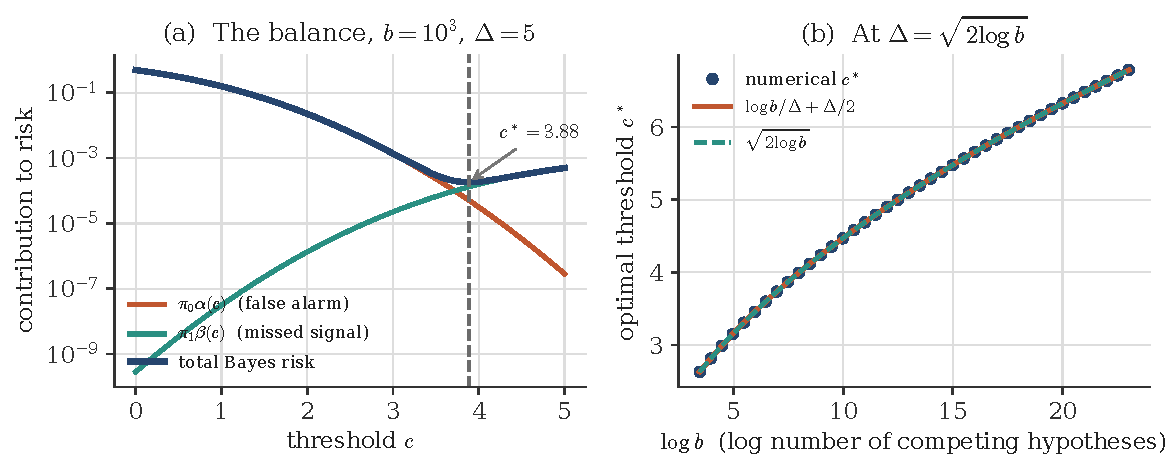
\includegraphics[width=0.9\textwidth]{app_bayestesting}
\caption{The Rubin and Sethuraman balance for a two point problem. (a) Prior weighted false alarm and
missed signal contributions and their total against the threshold, for $b=10^3$ and $\Delta=5$; the
risk optimal cutoff is where their derivatives cancel. (b) At the detectability boundary
$\Delta=\sqrt{2\log b}$, the numerical optimum, the closed form $\log b/\Delta+\Delta/2$, and
$\sqrt{2\log b}$ agree across more than eight orders of magnitude in $b$.}
\label{fig:app_bayestesting}
\end{figure}

\subsection{The sequential balance}\label{rs:sec:sequential}

The same balance chooses the threshold of a sequential test. Suppose each observation costs $\kappa$,
a false rejection costs $L_{10}$, and the test stops at $\tau_b$ of Theorem~\ref{ev:thm:stopping}.
Under the alternative it always stops, so there are no missed signals, only sampling costs; under the
null it stops, wrongly, with probability at most $1/b$, and otherwise runs forever at no cost in this
idealization.

\begin{proposition}[Sequential Rubin and Sethuraman threshold]\label{rs:prop:seq}
With these costs and the bounds of Theorem~\ref{ev:thm:stopping}, the Bayes risk satisfies
\[
R(b)\ \le\ \frac{\pi_0L_{10}}{b}+\pi_1\kappa\,\frac{\log b+C}{\mu},
\]
with $C$ the overshoot constant, and the right side is minimized at
$b^\ast=\pi_0L_{10}\,\mu/(\pi_1\kappa)$, where its value is
$(\pi_1\kappa/\mu)(1+C+\log b^\ast)$.
\end{proposition}

\begin{proof}
The first term is Ville's bound on the false rejection probability, the second Wald's identity for
the expected sample size under the alternative. Differentiate in $b$: $-\pi_0L_{10}/b^2+
\pi_1\kappa/(\mu b)=0$.
\end{proof}

The optimal threshold is the posterior odds cutoff $\pi_0L_{10}/\pi_1$ of
Theorem~\ref{ev:thm:canonical} scaled by $\mu/\kappa$, the information per unit cost. As each observation
becomes cheap, the expected sample size under the alternative grows like $\log(1/\kappa)/\mu$, the sequential counterpart of the
$\log n$ of Theorem~\ref{rs:thm:boundary}, while the risk falls like $\pi_1\kappa\log(1/\kappa)/\mu$; the sample size fluctuates on the $\sqrt{\log b^\ast}$
scale of Theorem~\ref{ev:thm:stopping}(iii). For the Bernoulli example of Section~\ref{ch:mdptest} with
equal prior odds, $L_{10}=1$ and $\kappa=10^{-4}$, the rule gives $b^\ast=457$ and an expected sample
size of about $(\log457)/0.0457\approx134$ observations under the alternative.

\subsection{Testing regions as sets}\label{ev2:sec:regions}

Stated for a scalar statistic the balance produces a number, but the argument never used the
scalarity. In general the testing region is a set $\mathcal R$ in the space of the statistic, and the
risk optimal choice is the set on which the weighted likelihood ratio exceeds one,
\eqref{rs:eq:rule}, which is the Neyman and Pearson region with the prior odds and losses supplying
the constant. Theorem~\ref{rs:thm:boundary} shows that near the null this region is the outside of a
sphere of radius $\sqrt{(k+\lambda)\log n/n}$ in Fisher coordinates, deformed by the direction factor
$h$; when the prior or loss favors some directions, the region bulges toward them.

The geometry of Section~\ref{ch:sanov} then supplies the error exponents. The probability that the
empirical distribution falls in $\mathcal R$ under the null is governed by the divergence from the
I projection of the null onto $\mathcal R$ to the null, and the same statement with the roles exchanged governs
the missed signal probability when the alternative is simple. For a composite alternative with prior $\Pi_1$ the missed signal probability is the average over $\Pi_1$ of the probabilities under $P_\theta$, and by the Laplace principle its exponent is the infimum over $\theta$ in the support of $\Pi_1$ of the divergence from the I-projection of $P_\theta$ onto the complement of $\mathcal R$ to $P_\theta$, for $\theta\mapsto P_\theta$ continuous. For a simple alternative, balancing the two weighted exponents is a statement about two
projections onto the common boundary of the region and its complement, and the optimal region is the one for which the two projections
are equidistant in divergence after prior weighting. At the moderate scale both divergences are
quadratic forms in the Fisher information, which is why the region is an ellipsoid there.

\paragraph{Summary.} Judge a test by its prior weighted risk and four facts follow. The Bayes rule is
a weighted likelihood ratio threshold. Its boundary sits at $n\|\hat\theta\|^2=(k+\lambda)\log n$ plus
lower order terms that matter in practice. The minimal risk is of order $(\log n/n)^{(k+\lambda)/2}$, almost all
of it missed signals near the null. And because all of this happens at moderate deviations, tests
compare through their Fisher informations, so Bayes risk efficiency is Pitman efficiency. In the two
point problem the balance reduces to $c^\ast=\log b/\Delta+\Delta/2$, and in a sequential problem to
$b^\ast=\pi_0L_{10}\mu/(\pi_1\kappa)$. No significance level enters anywhere.

\subsection*{Problems}
\begin{enumerate}[leftmargin=2.2em,itemsep=2pt]
\item Derive the Bayes rule \eqref{rs:eq:rule} from \eqref{rs:eq:risk} by minimizing pointwise in the data.
\item Prove Theorem~\ref{rs:thm:boundary} by a Laplace expansion, and identify where the condition
$\|\hat\theta\|\gg n^{-1/2}$ is used.
\item For $k=1$, $\lambda=0$ and a standard normal weight, show that the missed signal part of the
minimal risk is $2\phi(0)\sqrt{\log n/n}(1+o(1))$ and the false alarm part is smaller by a factor
$1/\log n$.
\item Show that loss $\ell(\theta)=\|\theta\|^2$ for a false acceptance raises the boundary from
$k\log n$ to $(k+2)\log n$, and explain why cheap near misses make the test more conservative.
\item Compute the Bayes risk efficiency of the sign test relative to the mean test under a logistic
law and under a Laplace law, and check the second against a simulation.
\item Derive the stationarity condition $b\,\phi(c)=\phi(c-\Delta)$ and solve it to obtain
\eqref{ev2:eq:cstar}. Show that at $\Delta=\sqrt{2\log b}$ the threshold is $\sqrt{2\log b}$ and
explain why the prior odds enter at leading order only in that case.
\item Prove Proposition~\ref{rs:prop:seq} and compute $b^\ast$ and the expected sample size for the
online calibration monitor of Section~\ref{ch:testpractice}.
\end{enumerate}

\src{Rubin and Sethuraman (1965a, 1965b) on probabilities of moderate deviations and Bayes risk
efficiency; Kallenberg (1983) on intermediate efficiency; Bahadur (1960) and Pitman (1948) for the two
classical efficiencies; Wald (1947) for the sequential cost balance. The boundary table, risk
decomposition and efficiency ratios were computed for the book.}


%====================================================================================================

\section{Testing in Practice: Experiments and Monitoring}\label{ch:testpractice}

\noindent\textbf{Thesis.} The calculus of this chapter makes three predictions that can be checked by
simulation: a likelihood ratio e-process keeps its false alarm rate under arbitrary optional stopping,
a statistic that looks like evidence but is not a supermartingale does not, and the detection time is
set by the divergence. This section checks all three and then runs the full calculus on an online
monitoring problem.

\subsection{Optional stopping under the null}\label{tp:sec:optional}

Test $p=0.5$ against $p=0.65$ with Bernoulli data. Under the null, monitor continuously and stop at
the first $t\le500$ at which the evidence reaches $20$, so the nominal false alarm rate is
$1/20=0.05$. Three evidence processes are compared over $10{,}000$ replications
(Figure~\ref{fig:tst_seq}(c)).
\begin{itemize}[leftmargin=1.6em,itemsep=2pt]
\item The likelihood ratio e-process $E_t=\prod_s(0.65/0.5)^{X_s}(0.35/0.5)^{1-X_s}$ rejects in
$4.5$ percent of runs (standard error $0.2$), inside Ville's bound.
\item The prequential mixture, the Krichevsky and Trofimov predictor with a
$\mathrm{Beta}(\tfrac12,\tfrac12)$ prior, divided by the null likelihood, is a Bayes factor and hence
a null martingale; it rejects in $3.7$ percent of runs. It pays a little in power for not knowing the
alternative and nothing in validity.
\item The maximum likelihood ratio $\sup_\theta p_\theta(X^t)/p_0(X^t)$ rejects in $21.8$ percent of
runs (standard error $0.4$), more than four times the nominal rate. It is the static code of
Theorem~\ref{ev:thm:lift} without its normalizer, and its logarithm grows like $\tfrac12\log t$ under
the null, which is the regret that a supermartingale cannot carry.
\end{itemize}
The second and third rows differ only in whether the alternative is integrated or maximized over,
which is the difference between a Bayes factor and a generalized likelihood ratio, and between a
prequential code and NML.

\subsection{Detection under the alternative}\label{tp:sec:detect}

Under $\mathrm{Bern}(0.65)$, $95$ percent of $500$ paths cross $\log20$ within $200$ observations, with
median stopping time $47$; the $200{,}000$ replications of Table~\ref{tab:tst_tau} give mean
$68.1$ and median $52$, against $(\log20)/\mu=65.6$. The mean exceeds the median because the stopping
time is right skewed at this small threshold, as Section~\ref{ch:mdptest} explained. The table of
Section~\ref{ch:mdptest} and the misspecification experiment complete the picture.

\subsection{Three calibrations of one test}\label{tp:sec:calibrations}

\begin{table}[t]
\centering\small
\begin{tabular}{@{}p{2.3cm}p{3.6cm}p{3.3cm}p{3.6cm}@{}}
\toprule
 & Validity only & Moderate deviation efficiency & Rubin and Sethuraman risk \\
\midrule
Guarantee & Ville, $\Pb_0(\sup_tE_t\ge b)\le1/b$ & $\E_1[\tau_b]=(\log b)/\mu+O(1)$ & minimal prior weighted risk\\
Acts on & $E_t$ & $\log E_t$, a random walk & weighted likelihood ratio\\
Threshold & $b=1/\alpha$, any & $b=1/\alpha$, any & $b^\ast$ or $t^2=(k+\lambda)\log n+\cdots$\\
Grows with $n$? & no & no & yes, like $\log n$\\
Needs a likelihood ratio? & no & yes & yes, and a prior and losses\\
\bottomrule
\end{tabular}
\caption{Three calibrations of the same evidence. The first certifies, the second times, the third
optimizes.}
\label{tab:tst_calib}
\end{table}

Table~\ref{tab:tst_calib} lines up the three ways of choosing the threshold. Ville certifies error
control for any threshold and says nothing about power. The moderate deviation stopping theorem says
how long a likelihood ratio test takes at a given threshold. The Rubin and Sethuraman balance says
which threshold to use, and it is the only one of the three in which the threshold moves with the
sample size. Lindley's paradox (Section~\ref{ch:deviations}) is the gap between the first and the third
for fixed samples.

\subsection{Online calibration monitoring}\label{tp:sec:monitor}

A deployed classifier issues probabilities $\hat p(X)$ for a binary outcome, and the null hypothesis
is that it remains calibrated: $Y_t\mid X_t\sim\mathrm{Bern}(\hat p(X_t))$. The three layers
instantiate as follows.

\emph{Representation.} An alternative $P_1$ describes the drift one fears, for example probabilities
shifted toward the base rate. The evidence is the likelihood ratio
$\Lambda_t=\prod_{s\le t}P_1(Y_s\mid X_s)/P_0(Y_s\mid X_s)$, canonical by
Theorem~\ref{ev:thm:canonical}; if the direction of drift is uncertain, a mixture over alternatives
keeps validity and buys robustness.

\emph{Validity.} $\Lambda_t$ is a null martingale, so the monitor may be checked after every
prediction, at the end of each shift, or when something looks wrong, and the false alarm probability
over the whole deployment is at most $1/b$.

\emph{Decision.} With a target false alarm rate $\alpha=0.01$ and an anticipated divergence of
$\mu=0.05$ nats per prediction under the drift, the expected detection time is
$\log(100)/0.05\approx92$ predictions plus a constant overshoot. If false alarms and late detection
have costs, Proposition~\ref{rs:prop:seq} replaces the arbitrary $\alpha$ by $b^\ast$. If the drift
goes in a direction the alternative did not anticipate, the evidence stalls rather than crossing,
and \eqref{md:eq:lundberg} bounds how often it crosses anyway; a monitor whose evidence stops
growing is itself a signal to revisit the alternative.

Each layer corresponds to a separate engineering decision, the model of drift, the certificate, and
the alert threshold, and the separation guarantees that changing one does not invalidate the others.

\subsection*{Problems}
\begin{enumerate}[leftmargin=2.2em,itemsep=2pt]
\item Reproduce the three false alarm rates of Section~\ref{tp:sec:optional} and add a fourth
process, the NML ratio normalized at the horizon $T=500$. Is it valid at the fixed time $T$? Under
optional stopping?
\item Show that $\log\sup_\theta p_\theta(X^t)-\log p_{1/2}(X^t)$ grows like $\tfrac12\log t$ under
the null, and relate the excess false alarm rate to the regret of Section~\ref{ch:mdl}.
\item For the calibration monitor, compute $b^\ast$ when a false alarm costs one hour of an engineer's
time and each miscalibrated prediction costs one thousandth of that.
\item Design a mixture alternative for the monitor that detects drift in either direction, and compare
its detection time with the correctly specified one by simulation.
\end{enumerate}

\src{Experiments of Bayes, E-values, and Testing (Polson, Sokolov and Zantedeschi, 2026a,
arXiv:2602.04146), recomputed for the book. The recomputed false alarm rates are $4.5$ and $21.8$
percent against $4.2$ and $22.5$ percent in the paper, the alternative crossing rate $95$ percent
against $97$, and under misspecification about one path in ten crosses, where the paper reports
none; the text reports the recomputed values.}


%====================================================================================================

\bookpart{Asymptotics, Computation, and Decision}\label{part:asymptotics}
{\let\clearpage\relax\let\cleardoublepage\relax \chapter{Posterior Asymptotics and the Gaussian Regime}\label{chap:asymptotics}}

Why is the posterior so often approximately Gaussian, and when is it not? This chapter answers both
questions with the machinery already built. The posterior obeys a large-deviation principle whose rate
is the relative entropy from the true distribution; the curvature of that rate function at its
minimum is the Fisher information, and the quadratic approximation is the Bernstein--von Mises theorem.

Reading asymptotics this way makes the Gaussian limit a consequence of the information geometry rather
than a separate miracle, and it makes the exceptions (singular models, boundary parameters, and
non-regular likelihoods) predictable. The martingale structure of the posterior and the merging of
opinions round out a picture in which large-sample Bayes is the local reading of the book's global rate
function.

\section[Bayesian Asymptotics]{Bayesian Asymptotics: Merging, Martingales, and Moderate Deviations}\label{ch:asymptotics}

\noindent\textbf{Thesis.} The whole asymptotic theory of Bayesian conditioning can
be read off one object, the local log-likelihood-ratio field
$Z_n(u)=\exp\{\ell_n(\theta_0+\delta_n^{-1}u)-\ell_n(\theta_0)\}$, whose limiting
shape fixes the form of the posterior, whose rate $\delta_n$ fixes its speed, and
into which the prior enters only as a reweighting the data overwhelm. This section
is the review-level synthesis of the book: it revisits the results proved in the
spine, de Finetti and Sanov (Sections~\ref{ch:types}--\ref{ch:sanov}), the tilted
master inequality (Section~\ref{ch:master}), the projected limit
(Section~\ref{ch:projected}), inverse Sanov (Section~\ref{ch:inverse}), the
moderate-deviation scale (Section~\ref{ch:hsmdp}), and the curvature of the rate
function (Section~\ref{ch:whengaussian}), through the single lens of the field $Z_n$, and
adds the longitudinal theory the spine does not treat: Blackwell--Dubins merging,
the martingale calculus of marginal likelihoods and Bayes factors, the
Jeffreys--Lindley paradox, semiparametric and mixed-normal limits, and a catalog
of open problems in growing dimension. Read cross-sectionally the field gives
Bernstein--von Mises; read longitudinally it gives merging; conditioned on a
constraint it gives the de Finetti--Sanov tilt. They are one object.

\subsection{Introduction}\label{ba:sec:intro}

Bayesian inference reduces, formally, to a single conditioning operation: given a prior
$\pi$ on a parameter $\theta\in\Theta$ and a model $\{P_\theta\}$, observation of data
$X^n=(X_1,\dots,X_n)$ produces the posterior $\pi(\cdot\mid X^n)$. The whole asymptotic
theory of this operation can be read off one object. Write $\ell_n(\theta)=\sum_{i\le n}
\log p(X_i\mid\theta)$ for the log-likelihood and define, around a point $\thn$ and at a
local rate $\delta_n$, the \emph{local log-likelihood-ratio field}
\begin{equation}\label{ba:eq:Zfield}
Z_n(u)\;=\;\exp\!\big\{\ell_n(\thn+\delta_n^{-1}u)-\ell_n(\thn)\big\},
\qquad u\in\R^d .
\end{equation}
The posterior for the local parameter $u=\delta_n(\theta-\thn)$ is, by Bayes' rule, the tilt
\begin{equation}\label{ba:eq:posttilt}
\pi_n(u\mid X^n)\;\propto\;\pi(\thn+\delta_n^{-1}u)\,Z_n(u).
\end{equation}
\emph{Bayesian posterior asymptotics is the asymptotics of this one field.} Its limiting shape
determines the form of the posterior, the rate $\delta_n$ its speed, and the prior contributes only
a continuous reweighting that the data eventually overwhelm. The classical theory is then a catalog
of the limits $Z_n$ can take and the rates that accompany them:

\begin{itemize}[leftmargin=1.6em,itemsep=2pt]
\item If $Z_n(u)\toL \exp\{u^\top\Delta-\half u^\top \Info u\}$ with $\Delta\sim\Ncal(0,\Info)$
(\emph{local asymptotic normality}, LAN), the tilt \eqref{ba:eq:posttilt} is asymptotically
Gaussian: this is the \emph{Bernstein--von Mises} theorem, $\delta_n=\sqrt n$
(\S\ref{ba:sec:bvm}).
\item If the limiting field is \emph{mixed} normal, $\Info$ random, one obtains local
asymptotic mixed normality (LAMN) and a random norming, the regime of Heyde--Johnstone
(\S\ref{ba:sec:beyond}).
\item If the field has a non-Gaussian limit (jump-type, support-dependent), the rate changes,
$\delta_n=n$ being typical; this is the non-regular class of Ibragimov and Has'minskii
(\S\ref{ba:sec:beyond}).
\item On the coarse scale, $\log Z_n$ is governed by relative entropy and one recovers
Schwartz consistency, the Clarke--Barron redundancy expansion, and Sanov's theorem
(\S\ref{ba:sec:lindley}, \S\ref{ba:sec:sanov}).
\item On the intermediate scale, between $\sqrt n$ and $n$, $\log Z_n$ obeys a
\emph{moderate deviation principle} with a universal Gaussian rate (\S\ref{ba:sec:mdp}).
\item Run forward in $n$, the normalizing constant of \eqref{ba:eq:posttilt}, the marginal
likelihood, is a martingale after division by the true likelihood, and ratios of marginal likelihoods are \emph{test martingales}
(\S\ref{ba:sec:martingale}).
\item If the predictive law induced by one prior is absolutely continuous with respect to that induced by the other, the
posteriors \emph{merge} (\S\ref{ba:sec:merging}); when the model is wrong the field concentrates at a
Kullback--Leibler projection (\S\ref{ba:sec:misspec}).
\end{itemize}

\noindent These are not separate theories but one theory at different resolutions of a single
information-theoretic object. Because $-n^{-1}\log Z_n(u)$ is an empirical relative entropy, the
Gaussian (BvM), moderate-deviation, and Sanov regimes are the quadratic, intermediate, and global
behavior of \emph{one} Kullback--Leibler functional; the prior enters only through where it charges
that functional, while the martingale and merging statements track the same functional forward in
$n$. This is the unification the section develops, organized throughout by the identity \emph{de
Finetti $+$ Sanov $=$ Bayes} (\S\ref{ba:sec:sanov}).

\paragraph{What is new, and what is surveyed.} The bulk of this section is expository, and the
classical asymptotic theory it organizes is also developed in the monographs of van der Vaart
(1998), Ghosh and Ramamoorthi (2003), and Ghosal and van der Vaart (2017). What those treatments do
not do, and what we offer, is to read the whole theory off the single local field \eqref{ba:eq:Zfield}
and its three resolutions of one relative-entropy functional. Within that frame three things are, to
our knowledge, new or newly packaged: (i) the explicit martingale calculus of marginal likelihoods
and Bayes factors and its translation into the language of $e$-values and anytime-valid inference
(\S\ref{ba:sec:martingale}); (ii) the recasting of the posterior moderate deviation principle, due to
Eichelsbacher and Ganesh (2002a), as the intermediate magnification of the same field, with the
$e$-value consequences of Polson, Sokolov and Zantedeschi (2026a, arXiv:2602.04146) (\S\ref{ba:sec:mdp}); and (iii) the
partial results of \S\ref{ba:sec:open}, in particular the proportional-asymptotic functional BvM
(Theorem \ref{ba:thm:prop}), the misspecified calibrating temperature (Proposition \ref{ba:prop:calib}),
and the mean-field anti-conservatism bound (Proposition \ref{ba:prop:vb}). Established results are
attributed in situ; everything else is survey.

\medskip
\noindent Table \ref{ba:tab:resolutions} previews the architecture: one field, read at four resolutions,
each with its own limit, governing theorem, and computational counterpart.

\begin{table}[h]
\centering\small
\renewcommand{\arraystretch}{1.25}
\begin{tabular}{@{}p{2.7cm}p{3.0cm}p{3.5cm}p{3.3cm}@{}}
\hline
Resolution & Limit of $Z_n$ & Governing result & Computation\\
\hline
Central limit \newline $\delta_n=\sqrt n$ & log-Gaussian (LAN) & Bernstein--von Mises
(\S\ref{ba:sec:bvm}) & Laplace, INLA\\
Moderate \newline $1\ll a_n\ll\sqrt n$ & Gaussian rate $\tfrac12 v^\top\Info v$ & moderate deviation
principle (\S\ref{ba:sec:mdp}) & exponential tilts, importance sampling\\
Large \newline speed $n$ & relative-entropy rate (Sanov) & de Finetti $+$ Sanov $=$ Bayes
(\S\ref{ba:sec:sanov}) & variational Bayes ($I$-projection), EP\\
Longitudinal \newline along $n$ & martingale & test martingale, Ville (\S\ref{ba:sec:martingale}) &
sequential Monte Carlo\index{sequential Monte Carlo}\\
\hline
\end{tabular}
\caption{The local likelihood-ratio field $Z_n$ at four resolutions: its limit, the governing
asymptotic statement, and the computation each scale licenses. Every row is one reading of the same
Kullback--Leibler functional.}
\label{ba:tab:resolutions}
\end{table}

\paragraph{Historical note and scope.} The threads we braid together have long, partly separate
histories: Laplace's large-sample normal approximation and its rigorous descendants through
Bernstein, von Mises, Le Cam, and van der Vaart; the Leningrad school's likelihood-ratio random
field (Ibragimov and Has'minskii) growing out of Linnik's program on maximum-likelihood asymptotics;
the merging and martingale strand from Doob, Blackwell--Dubins, and Diaconis--Freedman; the
information-theoretic strand from Lindley, Schwartz, Clarke--Barron, and Rissanen; and the
large-deviation strand from Sanov, Cram\'er, and Csisz\'ar. Our contribution is not new
foundations but a single vantage point, the local likelihood-ratio field and its rate function, from
which these appear as one theory, together with the martingale calculus of Bayes factors
(\S\ref{ba:sec:martingale}) and the moderate deviation principle (\S\ref{ba:sec:mdp}) that fills the scale
between the central-limit and large-deviation regimes. We restrict attention throughout to the
dominated, i.i.d.\ or weakly dependent setting; nonparametric and high-dimensional
extensions are surveyed in \S\ref{ba:sec:modern} and flagged as open where the finite-dimensional
picture breaks.

\paragraph{Notation.} $P_\thn$ denotes the data-generating law; $\E_0,\Prob_0$ expectation and
probability under it. For probability measures $\KL(Q\,\|\,P)=\int \log(dQ/dP)\,dQ$ is the
relative entropy (Kullback--Leibler divergence). $\Info(\theta)=\E_\theta[\nabla\log
p\,\nabla\log p^\top]$ is the Fisher information. The empirical measure of $X^n$ is
$\Pn=n^{-1}\sum_{i\le n}\delta_{X_i}$. We write $\toL$ for weak convergence and $\to_p$
for convergence in probability. A sequence obeys a large deviation principle (LDP) with speed
$n$ and rate $I$ if $-\inf_{A^\circ}I\le\liminf n^{-1}\log\Prob(\cdot\in A)
\le\limsup n^{-1}\log\Prob(\cdot\in A)\le-\inf_{\bar A}I$; a moderate deviation principle is the same statement at speed $a_n^2$.

\subsubsection{Foundations: exchangeability, sufficiency, and the posterior map}
\label{ba:sec:foundations}

Before magnifying the field we record the four structural facts the rest of the section rests on:
exchangeability forces the model, sufficiency compresses it, the likelihood principle fixes what the
data contribute, and Doob's theorem makes the posterior a process.

\paragraph{de Finetti's representation.}
The Bayesian model is not an extra assumption layered on a sampling model; for an
exchangeable sequence it is forced. If $(X_1,X_2,\dots)$ is an infinite exchangeable sequence
of $\Xcal$-valued random variables, de Finetti's theorem represents its law as a mixture of
i.i.d.\ laws,
\begin{equation}\label{ba:eq:definetti}
\Prob(X_1\in A_1,\dots,X_n\in A_n)\;=\;\int_{\Pcal(\Xcal)}\prod_{i=1}^n Q(A_i)\,\Pi(dQ),
\end{equation}
where the mixing measure $\Pi$ is the law of the almost-sure limit of the empirical measures
$\Pn$. Equation \eqref{ba:eq:definetti} \emph{is} a prior $\Pi$ over sampling distributions $Q$
together with i.i.d.\ sampling given $Q$. The parameter is, at bottom, the limiting frequency
$Q=\lim_n\Pn$; finite-dimensional parametrizations $\theta\mapsto P_\theta$ are sub-models of
this. We return to \eqref{ba:eq:definetti} in Section \ref{ba:sec:sanov}, where Sanov's theorem
supplies the exponential rate at which $\Pn$ concentrates and thereby the asymptotics of the
posterior $\Pi(\cdot\mid X^n)$.

\paragraph{Bayes sufficiency (Kolmogorov, 1942).}
The posterior is a function of the data only through a sufficient statistic, and Kolmogorov's
measure-theoretic formulation makes this the \emph{definition}. A statistic $T$ is
\emph{Bayes (Kolmogorov) sufficient} if for every prior $\pi$,
\begin{equation}
\pi\big(\theta\in\cdot \mid X^n\big)\;=\;\pi\big(\theta\in\cdot\mid T(X^n)\big)
\qquad\text{a.s.}
\end{equation}
This recasts Fisher--Neyman sufficiency as an invariance of the posterior map and is the
seed of the entire ``data $\mapsto$ posterior functional'' viewpoint: asymptotics studies the
behavior of this map as $n\to\infty$, and reduction by sufficiency is what makes the local
field \eqref{ba:eq:Zfield} a finite-dimensional object in regular problems. Kolmogorov's 1942
treatment of the Gauss model, center of dispersion and accuracy from a finite sample, is the
historical origin of the measure-theoretic posterior we now take for granted.

\paragraph{The likelihood principle and conditioning.}
Two further classical pillars sit beneath the posterior map. The likelihood principle, given a formal
basis by Birnbaum's (1962) derivation from sufficiency and conditionality, asserts that all evidential
content of the data about $\theta$ is carried by the likelihood function $\theta\mapsto
\prod_i p(X_i\mid\theta)$, up to a multiplicative constant. The Bayesian posterior \eqref{ba:eq:posttilt}
respects this automatically; it depends on the data only through the likelihood, which is why the
stopping rule that generated the data is irrelevant to the posterior and why the test-martingale
guarantees of \S\ref{ba:sec:martingale} can be anytime-valid: optional stopping does not alter the
likelihood and hence does not alter the posterior. Frequentist tail-area procedures, by contrast,
depend on the sample space and so violate the principle, which is the deeper source of the
Jeffreys--Lindley divergence of \S\ref{ba:sec:lindley}. The conditionality principle, that one should
condition on an ancillary statistic, is likewise built into conditioning on the observed data, and
the local field \eqref{ba:eq:Zfield} is the conditional object the principle prescribes. These
principles are the static, finite-$n$ counterparts of the asymptotic coherence that merging
(\S\ref{ba:sec:merging}) expresses in the limit.

\paragraph{The tail $\sigma$-field and Doob's theorem.}
Exchangeability ties the parameter to the tail. By the Hewitt--Savage zero--one law the exchangeable
(hence tail) $\sigma$-field of an i.i.d.-mixture sequence is trivial given $Q$, and de Finetti's $Q$
is itself measurable with respect to the tail: $Q=\lim_n\Pn$. Consistency is therefore the statement
that the parameter is recoverable from the tail, and Doob's theorem (Corollary \ref{ba:cor:doob}) is the
martingale expression of this recoverability, $\E[g(\theta)\mid\Fcal_n]\to g(\theta)$ a.s.\ because
$\theta$ is $\Fcal_\infty$-measurable. The fragility of merging in infinite dimensions
(\S\ref{ba:sec:merging}) is, dually, that two priors can disagree on tail events of probability
zero under one but positive under the other, so that the tail no longer determines the parameter in a
shared way. The whole longitudinal theory thus turns on the structure of the tail $\sigma$-field.

\paragraph{The posterior as a stochastic process in $n$.}
Fix an integrable functional $g(\theta)$ and consider the posterior means
$M_n=\E[g(\theta)\mid \Fcal_n]$, where $\Fcal_n=\sigma(X_1,\dots,X_n)$. By the tower property
$M_n$ is a martingale, and this single observation already yields a form of Bayesian
consistency (\S\ref{ba:sec:martingale}). Thus the posterior has two asymptotic faces: \emph{across}
the parameter at fixed large $n$ (the local field, \S\ref{ba:sec:bvm}), and
\emph{along} $n$ at fixed functionals (the martingale, \S\ref{ba:sec:merging}).
The remainder of the section develops both.

\subsection{Merging and martingales: the longitudinal view}\label{ba:sec:merging}

Two Bayesians who disagree on the prior but agree on which events are possible come to agree,
asymptotically, on predictions. This is the content of merging, and it is the probabilistic
backbone of the frequentist legitimacy of Bayesian methods. Informationally, when the two laws have finite relative entropy, it is the statement
that the relative entropy between the two predictive laws, accumulated one step at a time, is
almost surely finite, so the per-step divergence must vanish; merging is the convergence to zero
of a Kullback--Leibler increment, the same functional that reappears as Fisher curvature in
\S\ref{ba:sec:bvm} and as the Sanov rate in \S\ref{ba:sec:sanov}. Merging and the martingale calculus of
the next subsection are two faces of this longitudinal view: merging says the predictive laws
converge, and the martingale property of the marginal likelihood says \emph{how}: the evidence is a
fair game whose increments are the steps by which opinions merge.

\subsubsection{Blackwell--Dubins merging}
Let $\Prob$ and $\Q$ be two predictive laws on the sequence space
$(\Xcal^\infty,\Fcal_\infty)$, induced by two priors through the same model. Write
$\Prob_n(\cdot)=\Prob(\cdot\mid\Fcal_n)$ and $\Q_n$ for the one-step-ahead (indeed
all-future) conditional distributions.

\begin{theorem}[Blackwell--Dubins, 1962]\label{ba:thm:bd}
If $\Q$ is absolutely continuous with respect to $\Prob$ on $\Fcal_\infty$, then the
predictive distributions merge in total variation:
\begin{equation}
\sup_{A\in\Fcal_\infty^{(n)}}\big|\Prob(A\mid\Fcal_n)-\Q(A\mid\Fcal_n)\big|
\;\xrightarrow[n\to\infty]{}\;0\qquad \Q\text{-a.s.},
\end{equation}
where $\Fcal_\infty^{(n)}=\sigma(X_{n+1},X_{n+2},\dots)$ is the future after time $n$.
\end{theorem}

\begin{proof}[Sketch]
The Radon--Nikodym density $D_\infty=d\Q/d\Prob$ exists on $\Fcal_\infty$ by absolute
continuity. The densities $D_n=\E_\Prob[D_\infty\mid\Fcal_n]$ form a uniformly integrable
$\Prob$-martingale and converge to $D_\infty$ a.s.\ and in $L^1$ by L\'evy's upward theorem.
The total-variation gap between the conditional laws of the future is controlled by
$\E_\Prob[\,|D_\infty/D_n-1|\mid\Fcal_n]=\E_\Prob[\,|D_\infty-D_n|\mid\Fcal_n]/D_n$. Since $D_n\to D_\infty>0$ $\Q$-a.s.\ and $\Q\ll\Prob$,
it suffices that the numerator tends to $0$ $\Prob$-a.s. Fix a level $M$ and put $Y=D_\infty\wedge M$, $R=(D_\infty-M)^+$ and $W_m=\sup_{k\ge m}|Y-\E_\Prob[Y\mid\Fcal_k]|\le M$. For $n\ge m$ the numerator is at most $\E_\Prob[W_m\mid\Fcal_n]+2\E_\Prob[R\mid\Fcal_n]$, which tends to $W_m+2R$ by L\'evy's theorem. Letting $m\to\infty$ ($W_m\to0$ by L\'evy's theorem for the bounded $Y$) and then $M\to\infty$ through the integers sends this bound to $0$ off a countable union of null sets. Hence the future-conditioned laws coincide in the
limit.
\end{proof}

Theorem \ref{ba:thm:bd} is \emph{strong} merging: the agreement is over the entire infinite
future, uniformly, and almost surely. Its hypothesis, absolute continuity of $\Q$ with respect to $\Prob$ on $\Fcal_\infty$, is mild in
finite-dimensional models: when the model is identifiable, $\theta$ is $\Fcal_\infty$-measurable by
Doob's (1949) consistency theorem (Corollary \ref{ba:cor:doob}), so the hypothesis holds if and only if the prior
inducing $\Q$ is absolutely continuous with respect to the prior inducing $\Prob$, which is more than
overlapping support.

\begin{corollary}[Doob consistency]\label{ba:cor:doob}
If the model $\theta\mapsto P_\theta$ is identifiable and $\pi$ is any prior, then for
$\pi$-almost every $\thn$ the posterior $\pi(\cdot\mid X^n)$ concentrates at $\thn$ under
$P_\thn^\infty$. Consequently, when $\theta\mapsto P_\theta$ is continuous in total variation, the one-step posterior predictive merges weakly with the true predictive.
\end{corollary}

\paragraph{Weak versus strong merging, and a rate.}
It is useful to separate two notions. Two predictive laws \emph{merge strongly} if the
total-variation distance between their future-conditional laws tends to $0$ a.s.\ (Theorem
\ref{ba:thm:bd}); they \emph{merge weakly} if only finitely many predictive coordinates agree in
the limit, i.e.\ $|\Prob(X_{n+1}\in\cdot\mid\Fcal_n)-\Q(X_{n+1}\in\cdot\mid\Fcal_n)|\to0$. Strong
merging requires absolute continuity on the tail and is what fails in nonparametric models;
weak merging survives far more often and is the relevant notion for one-step prediction and
prequential calibration. The martingale proof of Theorem \ref{ba:thm:bd} also delivers a rate: if
$D_n\to D_\infty$ in $L^2$ at rate $\E_\Prob(D_\infty-D_n)^2=O(\rho_n)$, then the merging gap is
$O_p(\sqrt{\rho_n})$, and in regular finite-dimensional models $\rho_n\asymp n^{-1}$, so opinions
merge at the $n^{-1/2}$ rate of BvM; the cross-sectional and longitudinal rates coincide, as they
must, since both are governed by the same Fisher information.

\begin{example}[Two Bayesians on a coin]\label{ba:ex:coin}
Let $X_i$ be i.i.d.\ Bernoulli$(\theta)$ and let two analysts use $\mathrm{Beta}(a_1,b_1)$ and
$\mathrm{Beta}(a_2,b_2)$ priors. After $n$ trials with $s_n=\sum_i X_i$ successes, their posterior
means are $(a_j+s_n)/(a_j+b_j+n)$, which differ by $O(n^{-1})$, and the total-variation distance
between their $\mathrm{Beta}$ posteriors is $O(n^{-1/2})$, the merging rate of \S\ref{ba:sec:merging}.
Both priors have positive densities on $(0,1)$, so each is absolutely continuous with respect to the
other, and so are the predictive measures (full support alone would not suffice); Theorem \ref{ba:thm:bd} applies: the analysts' forecasts of all future tosses merge
almost surely. Merging fails if one analyst dogmatically assigns a point mass, e.g.\ a prior
$\delta_{1/2}$ that no data can move; the absolute-continuity hypothesis is what rules out
such dogmatism.
\end{example}

\paragraph{The prequential principle.}
Dawid's prequential principle reads the marginal likelihood as a sequence of genuine forecasts
$p(X_{i}\mid X^{i-1})$ to be scored as they are issued, and judges a Bayesian by the empirical
calibration of these forecasts rather than by the prior that generated them. Merging is then the
statement that two well-calibrated forecasters with mutually absolutely continuous predictive laws issue asymptotically
identical forecasts, and the martingale structure of \S\ref{ba:sec:martingale} is what makes the
running log-score $-\log m_n=-\sum_i\log p(X_i\mid X^{i-1})$ a meaningful cumulative loss whose
expected excess over the log-score of the true model is the redundancy \eqref{ba:eq:cb}. The prequential view thus unifies merging
(\S\ref{ba:sec:merging}), the martingale calculus (\S\ref{ba:sec:martingale}), and the
information-theoretic risk (\S\ref{ba:sec:info}) under a single forecasting criterion.

\paragraph{When merging fails.}
The almost-sure ``$\pi$-a.e.\ $\thn$'' in Corollary \ref{ba:cor:doob} is not a uniform statement,
and in infinite dimensions the null set can be large. Freedman (1963, 1965) exhibits, for i.i.d.\ sampling on a countable set, priors of full topological support whose posteriors are inconsistent at a dense set of
parameters, and shows that in the topological sense inconsistency is the generic case; Diaconis and Freedman (1986) give inconsistent Dirichlet process priors in a location problem: merging is a tail event and tail events are fragile under the weak topology. The
practical lesson is that strong merging (Theorem \ref{ba:thm:bd}) requires absolute continuity that
nonparametric priors routinely violate, and one must retreat to \emph{weak} merging, agreement
of finitely many predictive coordinates, or to rate statements (posterior contraction,
\S\ref{ba:sec:modern}). This dichotomy, automatic merging in regular finite-dimensional models,
delicate and prior-dependent merging in nonparametric ones, recurs throughout the section.

\paragraph{Merging and coherence.}
Merging is the asymptotic face of de Finetti's coherence: a coherent forecaster updates by
conditioning, and two coherent forecasters who never assign probability zero to what the other
deems possible are driven together by data. Lindley repeatedly emphasized this consequence as
the operational content of the Bayesian position; we take up his quantitative measure of how
fast information accrues in Section \ref{ba:sec:lindley}.

Merging also has a game-theoretic reading. In the rational-learning framework of Kalai and Lehrer,
players for whom the truth is absolutely continuous with respect to their subjective beliefs eventually
predict the future of a repeated game as well as if they knew it, and equilibrium play converges to
an approximate equilibrium of the true game; this is Theorem \ref{ba:thm:bd} applied to strategies
rather than parameters. The same absolute-continuity hypothesis, a ``grain of truth'', is what is
needed, and its failure is what produces persistent disagreement, both in inference and in strategic
learning.

\subsubsection{Martingale structure of marginal likelihoods and Bayes factors}
\label{ba:sec:martingale}

The normalizing constant of the tilt \eqref{ba:eq:posttilt} is, up to the factor $\delta_n^{d}/p(X^n\mid\thn)$, the marginal likelihood
\begin{equation}
m_n \;=\; \int_\Theta \prod_{i=1}^n p(X_i\mid\theta)\,\pi(d\theta)
\;=\; \prod_{i=1}^n p(X_i\mid X^{i-1}),
\end{equation}
a product of one-step predictive densities. This prequential factorization is the source of a
rich martingale calculus.

\paragraph{The marginal likelihood ratio is a martingale.}
Let $\pi_0,\pi_1$ be two proper priors (or two models) with marginal likelihoods
$m_n^{(0)},m_n^{(1)}$, and let the data be generated by the prior-predictive law
$\Prob_0$ of model $0$. The \emph{Bayes factor} is $B_n=m_n^{(1)}/m_n^{(0)}$.

\begin{proposition}\label{ba:prop:bf-mart}
Under $\Prob_0$, and provided the model-$1$ predictive law is absolutely continuous with respect to the model-$0$ one on each $\Fcal_n$ (otherwise $B_n$ is only a supermartingale), the Bayes factor process $(B_n)_{n\ge0}$ with $B_0=1$ is a nonnegative
martingale with $\E_0[B_n]=1$ for all $n$. Consequently $B_n$ converges $\Prob_0$-a.s.\ to a
finite limit $B_\infty$, and by Fatou $\E_0[B_\infty]\le 1$.
\end{proposition}

\begin{proof}
$B_n=dM_1^{(n)}/dM_0^{(n)}$ is the likelihood ratio of the two predictive measures restricted
to $\Fcal_n$. For any such ratio,
$\E_0[B_{n+1}\mid\Fcal_n]=B_n\,\E_0[\,p_1(X_{n+1}\mid X^n)/p_0(X_{n+1}\mid X^n)\mid\Fcal_n]=B_n$,
since the inner conditional expectation integrates the predictive ratio against the model-$0$
predictive density and equals one. Nonnegativity and Doob's martingale convergence theorem give
the a.s.\ limit; $\E_0[B_n]=\E_0[B_0]=1$.
\end{proof}

Proposition \ref{ba:prop:bf-mart} is the engine behind two modern developments.

\paragraph{Test martingales, Ville's inequality, and $e$-values.}
A nonnegative martingale $M_n$ with $M_0=1$ under a null $H_0$ is a \emph{test martingale}.
Ville's inequality,
\begin{equation}\label{ba:eq:ville}
\Prob_0\Big(\sup_{n\ge1} M_n \ge 1/\alpha\Big)\;\le\;\alpha,
\end{equation}
shows that rejecting $H_0$ when $M_n$ first exceeds $1/\alpha$ controls the type-I error at
level $\alpha$ \emph{simultaneously over all stopping times}, an anytime-valid test. By
Proposition \ref{ba:prop:bf-mart}, a Bayes factor against a simple-prior null \emph{is} a test
martingale when the model-$1$ predictive law is absolutely continuous with respect to the model-$0$ one on each $\Fcal_n$, and otherwise a \emph{test supermartingale} (a nonnegative supermartingale started at $1$), for which \eqref{ba:eq:ville} holds as well, so Bayesian model comparison inherits anytime validity for free: the posterior odds
may be inspected at every $n$ without inflating error. The terminal value $E=M_\tau$ at any
stopping time $\tau$ is an \emph{$e$-value}, a statistic with $\E_0[E]\le1$, and \eqref{ba:eq:ville}
is the $e$-value form of Markov's inequality. This places classical Bayes factors, the
likelihood-ratio identities of safe testing, and the optional-continuation guarantees of
$e$-processes within a single martingale frame.

\begin{remark}
The improper-prior case is where the martingale property can also break: with $\pi_1$
improper, $m_n^{(1)}$ is only defined up to an arbitrary constant and $B_n$ is no longer a
genuine likelihood ratio of probability measures. That arbitrary constant is Bartlett's (1957) objection to improper priors in testing, visible in \eqref{ba:eq:jl} as $\tau\to\infty$. The
Jeffreys--Lindley paradox itself (\S\ref{ba:sec:lindley}) needs no improper prior: it arises with a fixed proper prior as $n$ grows, through the
$\sqrt{n}$ Ockham factor.
\end{remark}

\paragraph{$e$-values, $e$-processes, and calibration.}
An \emph{$e$-process} is a nonnegative process $(E_n)$ such
that $E_n$ is upper-bounded by some test martingale at every stopping time, equivalently
$\E_0[E_\tau]\le1$ for all stopping times $\tau$; the test martingales above are $e$-processes.
Two properties make $e$-values the natural currency
of sequential Bayesian evidence. First, \emph{products combine evidence}: if $E,E'$ are $e$-values
from independent experiments then $EE'$ is an $e$-value, mirroring the multiplicativity of Bayes
factors. Second, \emph{$e$-values calibrate to $p$-values} and back: $1/E$ is a (conservative)
$p$-value by \eqref{ba:eq:ville}, while any admissible calibrator from $p$ to $e$ is a decreasing
function integrating to one. The martingale viewpoint thus gives Bayesian model
comparison an optional-continuation guarantee that fixed-$n$ $p$-values lack: one may keep sampling
until the evidence is decisive without inflating the error, because the test martingale's expectation
is pinned at one for all time.

\paragraph{Almost-sure growth and the iterated logarithm.}
The martingale convergence in Proposition \ref{ba:prop:bf-mart} concerns the Bayes factor under the
null. Under the alternative, the relevant statement is divergence at an exponential rate. If the
data are generated by a fixed $P_{\theta_1}$ in the Kullback--Leibler support of $\pi_1$ but outside the simple null $H_0:\theta=\thn$, then
$n^{-1}\log B_n\to \KL(P_{\theta_1}\|P_{\thn})>0$ a.s.\ by the law of large numbers applied to the
log-likelihood ratio, so the evidence accumulates linearly and the test is consistent. In a smooth parametric model with the density of $\pi_1$ positive and continuous at $\theta_1$, the mixture correction $\log\{m_n^{(1)}/p(X^n\mid\theta_1)\}$ is moreover $O(\log n)$ a.s., which Kullback--Leibler support alone does not ensure, and the
fluctuations around this drift then obey a law of the iterated logarithm: with $0<v^2<\infty$ the variance of the
per-observation log-likelihood ratio,
\begin{equation}
\limsup_{n\to\infty}\frac{\log B_n-n\,\KL(P_{\theta_1}\|P_{\thn})}{\sqrt{2 v^2 n\log\log n}}=1
\qquad\text{a.s.}
\end{equation}
The interplay of this a.s.\ linear drift under $H_1$ with the test-martingale boundedness under
$H_0$ is what makes sequential Bayesian tests both anytime-valid (\S\ref{ba:sec:martingale},
via Ville) and power-one: the boundary $1/\alpha$ is crossed with probability one under any fixed
alternative, while it is crossed with probability at most $\alpha$ under the null. The moderate
deviation analysis of \S\ref{ba:sec:mdp} interpolates between the central-limit fluctuations here and
the large-deviation drift, quantifying the evidence at thresholds growing slower than $n$.

\paragraph{Posterior means and martingale consistency.}
For an integrable $g$, $M_n=\E[g(\theta)\mid\Fcal_n]$ is a uniformly integrable martingale and
converges a.s.\ and in $L^1$ to $\E[g(\theta)\mid\Fcal_\infty]$ by L\'evy's theorem. If the
parameter is identified by the tail $\sigma$-field, guaranteed by Corollary \ref{ba:cor:doob} in
regular models, then $\E[g(\theta)\mid\Fcal_\infty]=g(\thn)$ and the posterior mean is
strongly consistent. Thus consistency, merging (Theorem \ref{ba:thm:bd}), and the calibration of
Bayes factors (Proposition \ref{ba:prop:bf-mart}) are three corollaries of one martingale
convergence theorem applied to three functionals: the density ratio, the future indicator, and
$g$.

%%---- incorporated: critique of martingale posteriors ----------------
\subsection[A Critique of Martingale Posteriors]{A Critique of Martingale Posteriors: Admissibility and the Moment Hierarchy}
\label{sec:mp-critique}

\noindent\textbf{Thesis.} The martingale-posterior construction of Fong, Holmes
and Walker (2023), introduced in Section~\ref{ev:sec:landscape} as the predictive
completion of the evidence martingale, imposes coherence on the first predictive
moment alone. Rewritten through the tower property the defining condition is
$\E[\theta_\infty\mid Y_{1:n}]=\theta_n$, a constraint on the conditional mean and
on nothing else, so, given only the value $\theta_n$, every conditional moment of order two and higher is free. Three
classical results turn that single observation into a critique. The complete-class
theorem ties admissibility to prior representations, the empirical plug-in has no proper one,
and under log-loss a Bayes predictive dominates it for every $\theta\in(0,1)$; the Kreps (1988) moment hierarchy shows that fixing the first moment
leaves every run probability of length two or more set-valued; and log-loss
minimax theory identifies the $\mathrm{Beta}(\tfrac12,\tfrac12)$ predictor, not the
plug-in, as worst-case optimal to leading order. This section is the destructive
counterpart to the constructive predictive theory of Sections~\ref{ch:master}
and~\ref{ch:moment}: conditioning on empirical moments through the $I$-projection
selects a unique predictive, whereas conditioning on the first moment
alone does not.

\subsubsection{Predictive Bayes: The Hahn--Martin--Walker Framework}

Hahn, Martin and Walker (2018)\ establish the theoretical foundations for \emph{predictive Bayes}: the program
of conducting posterior inference through coherent predictive distributions rather than
directly through prior-likelihood pairs.
Their key insight is that the posterior is fully characterized by the sequence of
one-step-ahead predictive conditionals, provided these satisfy an appropriate
coherence condition.

\textbf{The HMW setup.}\;
Let $Y_1, Y_2, \ldots$ be an observable sequence taking values in a space $\mathcal{Y}$.
A \emph{predictive system} is a sequence of conditional distributions
$\{Q_n(\cdot\mid y_{1:n-1})\}_{n\ge 1}$ where $Q_n$ specifies the predictive
distribution of $Y_n$ given the observed history $y_{1:n-1}$.
HMW require these predictive distributions to be \emph{coherent}: there exists an
exchangeable probability measure $P$ on $\mathcal{Y}^\infty$ such that $Q_n(\cdot\mid y_{1:n-1})$
equals the conditional distribution of $Y_n$ under $P$ given $Y_{1:n-1}=y_{1:n-1}$.
Exchangeability gives the condition its content, since by the Ionescu-Tulcea theorem every sequence of predictive kernels is the conditional system of some joint law.

Under coherence, the predictive system uniquely determines the full joint law of
$(Y_1, Y_2, \ldots)$.
For exchangeable sequences, de~Finetti's theorem guarantees that this joint law has the
representation
\begin{equation}\label{crit:eq:definetti}
 P(Y_1\in A_1,\ldots,Y_n\in A_n)
 = \int \prod_{i=1}^n F_\theta(A_i)\,\dPi,
\end{equation}
where $\Pi$ is the unique de~Finetti prior on the parameter $\theta$ indexing the
one-dimensional marginal $F_\theta$.
The prior $\Pi$ is thus recovered from the predictive system: it is the law of
$\theta = \lim_{n\to\infty}\hat F_n$, the weak limit of the empirical measure.

\textbf{The predictive posterior.}\;
HMW show that the posterior distribution of $\theta$ given $Y_{1:n}$ is determined by
the predictive system as
\begin{equation}\label{crit:eq:predpost}
 \Pi(\theta\mid Y_{1:n}) \;\propto\;
 \Pi(\theta)\prod_{i=1}^n q_\theta(Y_i\mid Y_{1:i-1}),
\end{equation}
where $q_\theta$ is the predictive density under model $\theta$.
The correspondence behind the HMW program is classical. A coherent predictive system, one satisfying the
coherence relation $\E[f(Y_{n+1})\mid Y_{1:n}] = \int f\,dQ_{n+1}(\cdot\mid Y_{1:n})$
for all bounded $f$ under an exchangeable $P$, determines $P$, hence by de~Finetti's theorem the prior $\Pi$ and every posterior
$\Pi(\theta\mid Y_{1:n})$ in \eqref{crit:eq:predpost}, and $\Pi$ determines the system in turn (Fortini, Ladelli and Regazzini, 2000).
Coherent predictive systems are thus in bijection with priors, and so with their sequences of posteriors.

\textbf{The HMW contribution in context.}\;
The HMW framework establishes three important facts for our purposes.
First, the posterior is not a primitive; it is derived from the predictive system.
Second, the prior $\Pi$ is not a modeling choice; it is the de~Finetti measure of the
observable sequence, recovered from the predictive distributions.
Third, the martingale property of the predictive means is a \emph{consequence} of
coherence, not a characterization of it: for integrable observations the predictive means
$\int y\,dQ_{n+1}(y\mid Y_{1:n})$ of every coherent system form a martingale, since exchangeability gives $\E[Y_{n+2}\mid Y_{1:n}]=\E[Y_{n+1}\mid Y_{1:n}]$ (the c.i.d.\ property of Remark~\ref{crit:rem:cid} is enough),
but the converse fails; many predictive
sequences with martingale means, such as c.i.d.\ sequences that are not exchangeable, are not coherent.

% ── 3. The FHW Martingale Posterior ───────────────────────────────────────────
\subsubsection{The FHW Martingale Posterior as a Weakening of HMW}

Fong, Holmes and Walker (2023)\ extend the HMW framework by relaxing the coherence requirement.
Rather than requiring the full predictive system to be coherent in the HMW sense,
they require only a martingale condition on the sequence of parameter estimates.

\textbf{The FHW construction.}\;
Define a sequential estimator $\theta_N=\theta(Y_{1:N})$ and take the
\emph{martingale posterior} to be the law of $\thoo=\lim_{N\to\infty}\theta_N$.
The sole requirement is:
\begin{equation}\label{crit:eq:mart}
 \E[\theta_N \mid Y_{1:N-1}] = \theta_{N-1} \quad \text{a.s.}
\end{equation}
Doob's theorem guarantees $\theta_N\to\thoo$ a.s.\ under boundedness.
When the predictive sequence arises from a proper prior via Bayes' rule, the martingale
posterior coincides with the conventional posterior, so FHW recover the HMW framework
as a special case.
They then propose \eqref{crit:eq:mart} as a sufficient substitute for HMW coherence.

\textbf{What FHW retain and what they discard.}\;
The HMW framework requires the predictive system $\{Q_n\}$ to be fully coherent: the
predictive distributions must be consistent with an exchangeable joint law $P$ and hence with a
de~Finetti prior $\Pi$.
FHW retain only the martingale condition \eqref{crit:eq:mart} on the parameter estimates,
discarding the requirement that the full predictive distributions be coherent.
This is a strict weakening: every HMW-coherent system satisfies \eqref{crit:eq:mart} with $\theta_N$ its predictive mean, but
many systems satisfying \eqref{crit:eq:mart} are not HMW-coherent.

\begin{remark}[c.i.d.\ sequences]\label{crit:rem:cid}
FHW work with \emph{conditionally identically distributed} (c.i.d.) sequences,
requiring $\E[f(Y_{n+k})\mid Y_{1:n}]=\E[f(Y_{n+1})\mid Y_{1:n}]$ for all $k\ge 1$ and bounded $f$.
Every c.i.d.\ sequence is asymptotically exchangeable; $F_n$ converges a.s.\ to the
de~Finetti measure.
However, c.i.d.\ does not imply exchangeability at any finite $n$, and the martingale
condition \eqref{crit:eq:mart} is weaker still; it is a consequence of c.i.d.\ but
constrains only the conditional mean of $\theta_N$, not in general the full conditional
distribution of $Y_{n+1}$ given $Y_{1:n}$.
\end{remark}

\textbf{Terminal-value rewriting (our contribution).}\;
The tower property applied to \eqref{crit:eq:mart} yields the equivalent condition:
\begin{equation}\label{crit:eq:tower}
 \E[\thoo \mid Y_{1:n}] = \theta_n \quad \text{a.s., for all }n.
\end{equation}
This reveals the content of the FHW condition.
In the HMW framework, the posterior $\Pi(\theta\mid Y_{1:n})$ encodes every conditional
moment of $\theta$ given $Y_{1:n}$.
Given only the current value $\theta_n$, the FHW condition \eqref{crit:eq:tower} encodes only the \emph{first} conditional moment;
conditional moments of order $\ge 2$ are not determined by it.
The gap is sharp: Polson and Zantedeschi (2026a) prove that for any martingale path
$(\theta_n)$ with values in $(0,1)$ and any $k\ge 2$, infinitely many priors on the parameter space have posterior mean equal to its current value $\theta_n$ and so are consistent
with it, not all assigning the same $k$-step predictive probability.

\textbf{The empirical predictive.}\;
The leading FHW instance sets $P(Y_{n+1}\le y\mid Y_{1:n})=F_n(y)$, the empirical CDF,
giving $P(X_{n+1}=1)=S_n/n$ in the binary case.
Predictive resampling from it updates $S_n/n$ after each imputed draw, a P\'olya urn, so
for $0<S_n<n$ the martingale posterior of $\theta$ is $\Bdist(S_n,n-S_n)$, the Bayesian
bootstrap (Rubin, 1981), which is also the posterior under the improper Haldane prior
$\Bdist(0,0)$; its $k$-step predictives are therefore determined, and the moment gap
below concerns condition \eqref{crit:eq:mart} alone.
The admissibility implications are not addressed by FHW.

% ── 4. Blackwell Admissibility ────────────────────────────────────────────────
\subsubsection{Blackwell Admissibility}

\begin{theorem}[Complete-class theorem; Wald, Le Cam]\label{crit:thm:blackwell}
Under suitable regularity, every admissible rule is Bayes for some prior $\Pi$, possibly
improper, or a limit of Bayes rules in risk; conversely, a unique Bayes rule for a proper prior with
finite Bayes risk is admissible. The converse for improper priors and risk-limits requires
additional conditions.
\end{theorem}

The minimax rule is Bayes for the \emph{least favorable prior}, the prior maximizing
Bayes risk.
Every admissible rule has a prior, possibly improper, or is a limit of Bayes rules; every rule with neither is risk-dominated.
In the HMW framework, every coherent predictive system corresponds to a prior $\Pi$
and hence every HMW-coherent predictor that is the unique Bayes rule for $\Pi$, with finite Bayes risk, is admissible.
The FHW relaxation admits predictors with no prior representation, and those that are not limits of Bayes rules are
inadmissible.

% ── 5. The Kreps Moment Hierarchy ─────────────────────────────────────────────
\subsubsection{The Kreps Moment Hierarchy}

\textbf{De Finetti and predictive moments.}\;
By de~Finetti's theorem, every exchangeable binary sequence satisfies
\begin{equation}\label{crit:eq:definetti_binary}
 P(X_1=x_1,\ldots,X_n=x_n)
 = \int_0^1 \theta^{s_n}(1-\theta)^{n-s_n}\,\dPi, \qquad s_n=\textstyle\sum x_i,
\end{equation}
where $\Pi$ is the unique de~Finetti prior on $\theta\in[0,1]$.
In the HMW framework, $\Pi$ is recovered from the coherent predictive system.
Given only the value of the path before any data, the FHW martingale condition constrains only $\mu_1=\E_\Pi[\theta]$,
leaving all higher moments of $\Pi$ undetermined.

\textbf{Kreps's observation.}\;
One failure requires only the prior mean: $P(X_1=0)=1-\E_\Pi[\theta]$.
Four consecutive failures require the fourth moment:
\begin{equation}\label{crit:eq:fourrun}
 P(X_1=X_2=X_3=X_4=0)
 = \E_\Pi[(1-\theta)^4]
 = 1 - 4\E[\theta] + 6\E[\theta^2] - 4\E[\theta^3] + \E[\theta^4].
\end{equation}
The $k$-step run probability is
\begin{equation}\label{crit:eq:krun}
 P(X_1=\cdots=X_k=0)
 = \E_\Pi[(1-\theta)^k]
 = \sum_{j=0}^{k}\tbinom{k}{j}(-1)^j \E[\theta^j].
\end{equation}
Predicting a run of length $k$ requires the first $k$ prior moments; no fewer suffice.
The HMW framework, by requiring coherence with a proper prior, encodes all moments.
The FHW framework requires only \eqref{crit:eq:mart}, and the current value $\theta_n$ then encodes only the first.

\textbf{The moment-gap theorem.}\;
Via \eqref{crit:eq:krun}, the $k$-step predictive requires
$\E[(1-\thoo)^k\mid Y_{1:n}]$.
Condition \eqref{crit:eq:tower} fixes only $\E[\thoo\mid Y_{1:n}]=\theta_n$.

\begin{proposition}[Moment-gap; Polson and Zantedeschi, 2026a]\label{crit:prop:gap}
For any first-moment martingale path $(\theta_n)_{n\ge 1}$ with values in $(0,1)$ satisfying \eqref{crit:eq:mart}
and any $k\ge 2$, the current value alone does not fix the $k$-step run probability: the map $\theta_n\mapsto \E[(1-\thoo)^k\mid Y_{1:n}]$ is set-valued, since
infinitely many priors $\Pi$ on $[0,1]$ have posterior mean $\theta_n$ given $Y_{1:n}$, and they
do not all assign the same $k$-step run probability. The whole path, given as a function of every history with $\theta_{n+1}$ taking different values after $Y_{n+1}=0$ and $Y_{n+1}=1$, does fix it, since \eqref{crit:eq:mart} then determines every predictive $P(Y_{n+1}=1\mid Y_{1:n})$.
\end{proposition}

\begin{corollary}[Predictive variance gap]\label{crit:cor:sequential}
Under the FHW condition \eqref{crit:eq:mart}, given only the current value $0<\theta_n<1$ and with $k\ge 2$, the predictive variance of the next $k$ observations, which for an exchangeable sequence is
\begin{equation}\label{crit:eq:predvar}
 \Var(X_{n+1}+\cdots+X_{n+k}\mid X_{1:n})
 = k\,\E[\thoo(1-\thoo)\mid X_{1:n}] + k^2\Var(\thoo\mid X_{1:n}),
\end{equation}
is not determined: $\Var(\thoo\mid X_{1:n})$ requires the second conditional moment
$\E[\thoo^2\mid X_{1:n}]$, which \eqref{crit:eq:tower} does not constrain and which enters with coefficient $k^2-k$ (for $k=1$ it cancels, leaving $\theta_n(1-\theta_n)$).
The coverage of any prediction set $C$ for $X_{n+1}+\cdots+X_{n+k}$ derived from the FHW martingale
posterior, if $C$ contains some but not all of $\{0,\dots,k\}$, is indeterminate too, and not because of the variance alone: it is the conditional mean of $\Prob(\mathrm{Bin}(k,\thoo)\in C)$, which for $k\ge2$ is not affine in $\thoo$.
\end{corollary}

The Hausdorff moment problem provides the algebraic certificate:
$\{\mu_k=\E[\theta^k]\}_{k\ge 0}$ is the moment sequence of a probability measure on
$[0,1]$ iff it is completely monotone.
A coherent system of run probabilities for all $k\ge 1$ is in exact bijection with a
valid prior $\Pi$, the de~Finetti measure recovered by HMW coherence.
Given only the value of the path before any data, the FHW martingale condition contributes only $\mu_1$; the truncated Hausdorff moment problem
stays indeterminate for every $k\ge 2$.

% ── 6. Blackwell (1995): Minimax Equals Bayes ─────────────────────────────────
\subsubsection{Blackwell (1995): Minimax versus Bayes}

\textbf{The minimax prediction problem.}\;
Blackwell (1995) asks how to predict an arbitrary deterministic binary sequence
$x=(x_1,x_2,\ldots)\in\{0,1\}^\infty$, adversarially chosen.
On day $n$, observe $h_n=(x_1,\ldots,x_{n-1})$ and predict $x_n$ under zero-one
loss.
Minimize worst-case long-run error, no prior, no likelihood, no exchangeability.

\textbf{The Blackwell algorithm and regret bound.}\;
Blackwell's minimax predictor randomizes: on every sequence its error rate is almost surely
at most $\min(\hat\theta_n,1-\hat\theta_n)+o(1)$, where $\hat\theta_n=s_n/n$ and the
minimum is the error rate of the best constant prediction in hindsight.
The rule this section sets against the plug-in is the Jeffreys predictor, which assigns
\begin{equation}\label{crit:eq:blackwellalg}
 p_n = \frac{s_{n-1}+\tfrac{1}{2}}{n}
\end{equation}
to $x_n=1$.
Scored by log-loss, with $p_t(1)=p_t$ and $p_t(0)=1-p_t$, it satisfies on every sequence
\begin{equation}\label{crit:eq:regret}
 \frac{1}{n}\sum_{t=1}^n \log\frac{1}{p_t(x_t)}
 \;\le\; H(\hat\theta_n) + \frac{\log n}{2n} + O(n^{-1}),
\end{equation}
where $H(\hat\theta_n)=-\hat\theta_n\log\hat\theta_n-(1-\hat\theta_n)\log(1-\hat\theta_n)$ is
the log-loss of the best fixed i.i.d.\ Bernoulli predictor in hindsight.
The worst case is a constant sequence, and the regret $\tfrac12\log n+O(1)$ has the minimax
order (Shtarkov, 1987).
Used as a randomized zero-one predictor, \eqref{crit:eq:blackwellalg} is not Blackwell's: on an
i.i.d.\ Bernoulli($\theta$) sequence it errs at rate about $2\theta(1-\theta)$, above
$\min(\theta,1-\theta)$ unless $\theta\in\{0,\tfrac12,1\}$.

\textbf{The triple identity.}\;
The predictor \eqref{crit:eq:blackwellalg} equals two independently
derived predictors and, under cumulative log-loss, approximates the minimax one:
\begin{equation}\label{crit:eq:triple}
 p_n
 = \frac{s_{n-1}+\tfrac{1}{2}}{n}
 \;=\;\underbrace{\text{Hill's }A_{(n)}}_{\text{rank symmetry}}
 \;=\;\underbrace{\mathrm{Bayes}\!\left[\Bdist\!\left(\tfrac{1}{2},\tfrac{1}{2}\right)\right]}_{\text{Jeffreys prior}}
 \;\approx\;\underbrace{\text{Minimax}}_{\text{least favorable prior.}}
\end{equation}
The last relation is asymptotic: the exact minimax predictor for cumulative log-loss is
Shtarkov's normalized maximum likelihood, with regret $\tfrac12\log(n\pi/2)+o(1)$; the
regret of \eqref{crit:eq:blackwellalg} exceeds it by $\tfrac12\log 2+o(1)$, and the
Jeffreys prior is asymptotically least favorable (Clarke and Barron, 1994).
Coherence alone admits every de~Finetti measure; within the HMW framework, applied to the
binary exchangeable case, rank symmetry and asymptotic least favorability select the
Jeffreys prior $\Bdist(\tfrac12,\tfrac12)$.
The FHW framework, constraining only \eqref{crit:eq:mart}, cannot make this selection.

\textbf{Sub-minimaxity of the FHW martingale posterior.}\;
The FHW plug-in, which retains only \eqref{crit:eq:tower}, is not merely inadmissible under log-loss
(Example~\ref{crit:ex:binary}); it is \emph{sub-minimax}: dominated by
\eqref{crit:eq:blackwellalg} on adversarially chosen sequences, with no probabilistic model
assumed.
In the worst case the gap is unbounded under log-loss, since the plug-in can give probability $0$ to the next outcome while \eqref{crit:eq:regret} holds on every sequence, and it is $\Omega(1)$ per round under zero-one loss (Failure~3 below).

% ── 7. Hill's A(n) Rule ───────────────────────────────────────────────────────
\subsubsection{Hill's \texorpdfstring{$A_{(n)}$}{A(n)} Rule: The HMW-Coherent Benchmark}

Hill (1968) proposed $A_{(n)}$ for continuous data: assign equal predictive probability $1/(n+1)$ to each
of the $n+1$ rank intervals defined by the order statistics.
Binary data are tied, and $A_{(n)}$ then bounds $P(X_{n+1}=1\mid X_{1:n})$ only between $S_n/(n+1)$ and $(S_n+1)/(n+1)$, since one of the $n+1$ intervals may go to either value; the binary form used here is the midpoint,
\begin{equation}\label{crit:eq:hill}
 P_{A_{(n)}}(X_{n+1}=1\mid X_{1:n}) = \frac{S_n+\tfrac{1}{2}}{n+1},
\end{equation}
which is also the posterior predictive under the Jeffreys prior $\Bdist(\tfrac12,\tfrac12)$.
Hill (1988) observed that $A_{(n)}$ ``is supported by all of the serious approaches to statistical
inference'': it is Bayesian, fiducial, and even a confidence or tolerance procedure.
Log-loss minimax theory adds a fourth endorsement: \eqref{crit:eq:hill} is minimax to leading order (Shtarkov, 1987; Clarke and Barron, 1994).
All roads lead to \eqref{crit:eq:triple}.

In the HMW framework, $A_{(n)}$ is a coherent predictive system for binary
exchangeable sequences that is also minimax to leading order: it corresponds to the Jeffreys
prior $\Bdist(\tfrac12,\tfrac12)$, which is the de~Finetti measure recovered by HMW
coherence applied to the rank-symmetric predictive system.
The $k$-step posterior predictive under $A_{(n)}$ is
\begin{equation}\label{crit:eq:an_kstep}
 P_{A_{(n)}}(X_{n+1}=\cdots=X_{n+k}=0\mid X_{1:n})
 = \prod_{j=0}^{k-1}\frac{n-S_n+\tfrac12+j}{n+1+j},
\end{equation}
encoding all posterior moments and delivering correct $k$-step run probabilities for
all $k\ge 1$.
The FHW martingale posterior, constrained only by \eqref{crit:eq:tower}, cannot recover
\eqref{crit:eq:an_kstep} for $k\ge 2$ without additional specification.

% ── 8. Application: Binary Counterexample ─────────────────────────────────────
\subsubsection{Application: Binary Prediction as a Counterexample}
\label{crit:sec:applications}

We now collect the preceding results into a single concrete counterexample.
Let $X_1,X_2,\ldots$ be i.i.d.\ $\mathrm{Ber}(\theta)$, $\theta\in(0,1)$ unknown.
We compare three predictors:
the \emph{FHW plug-in} $\hat\delta^{\mathrm{FHW}}$ using $S_n/n$;
the \emph{Bayes rule} $\delta^{\mathrm{Bayes}}$ under $\Bdist(\alpha,\beta)$;
and the \emph{Jeffreys--Hill rule} $\delta^*=A_{(n)}$,
corresponding to the Jeffreys prior $\Bdist(\tfrac12,\tfrac12)$.

\begin{example}[Binary prediction counterexample]\label{crit:ex:binary}
The FHW empirical plug-in fails three criteria simultaneously.
\end{example}

\textbf{Failure 1: Inadmissibility under log-loss.}\;
Under $\Bdist(\alpha,\beta)$ the Bayes predictive is
\begin{equation}\label{crit:eq:bayes}
 P_{\mathrm{Bayes}}(X_{n+1}=1\mid X_{1:n})
 = \frac{\alpha+S_n}{\alpha+\beta+n}
 = \frac{S_n}{n} + O(n^{-1}).
\end{equation}
Under log-loss, for every proper prior $\Pi$ on $(0,1)$ the Bayes rule $\delta^{\Pi}$ for $\Pi$, its posterior predictive, has Bayes risk $r(\Pi,\delta^{\Pi})\le\log 2$,
while $r(\Pi,\hat\delta^{\mathrm{FHW}})=\infty$: after $S_n=0$, an event of positive probability, the plug-in gives probability $0$ to $X_{n+1}=1$, which then has positive probability.
Under squared error loss the plug-in is admissible (below) and has only an excess Bayes risk; under the Jeffreys prior $\Bdist(\tfrac12,\tfrac12)$ the excess is
\begin{equation}\label{crit:eq:risk_gap}
 r\!\left(\Bdist(\tfrac12,\tfrac12),\hat\delta^{\mathrm{FHW}}\right)
 - r\!\left(\Bdist(\tfrac12,\tfrac12),\delta^*\right)
 = \frac{1}{8n(n+1)} > 0,
\end{equation}
an identity for every $n$, so the gap is $\Theta(n^{-2})$ and does not vanish faster.
The plug-in has no proper prior representation (it places a Dirac mass at the shifting
$S_n/n$); it remains admissible under squared-error loss, since it is the unique Bayes rule, with finite Bayes risk $1/n$, of the uniform prior under the weighted loss $(a-\theta)^2/\{\theta(1-\theta)\}$, which has the same admissible rules (equivalently, the generalized Bayes rule of the improper Haldane prior $\Bdist(0,0)$ under squared error),
but under squared error itself it is the Bayes rule of no proper prior, and under log-loss it is inadmissible, as the failures below show.
In the HMW framework, this corresponds to using a degenerate predictive system with no
de~Finetti measure; in the FHW framework, this deficiency is invisible because
\eqref{crit:eq:mart} is still satisfied.

The plug-in incurs an additional failure, an inadmissibility under log-loss.
\emph{Log-score dominance}: after an extreme run the plug-in assigns probability 0 or 1
to $X_{n+1}$, incurring infinite log-loss on any surprise; the Bayes predictive
\eqref{crit:eq:bayes} is bounded away from 0 and 1 and dominates for all $\theta\in(0,1)$.

\textbf{Failure 2: Moment gap.}\;
Held at $S_n/n$, as if $\theta$ were known, the plug-in predicts $k$ consecutive failures as $(1-S_n/n)^k$; FHW predictive resampling, a P\'olya urn, gives $\prod_{j=0}^{k-1}(n-S_n+j)/(n+j)$ instead.
The correct posterior predictive under $\delta^*=A_{(n)}$ is \eqref{crit:eq:an_kstep}.
The relative error between the plug-in and $A_{(n)}$, for $(n-S_n)/n$ bounded away from $0$, is
\begin{equation}\label{crit:eq:relerr}
 \frac{P_{A_{(n)}}(\text{$k$ failures}\mid X_{1:n}) - (1-S_n/n)^k}
 {P_{A_{(n)}}(\text{$k$ failures}\mid X_{1:n})}
 = O\!\left(\frac{k^2}{n}\right),
\end{equation}
which grows quadratically in run length $k$ and vanishes only as $n\to\infty$.
For any fixed $n$, the plug-in gets every run probability wrong for $k\ge 2$.

\emph{Numerical illustration.}
Fix $\E[\theta]=\tfrac12$, $n=10$, $S_n=5$.
Under $\Bdist(1,1)$: $P(\text{4 failures})\approx0.092$.
Under $\Bdist(5,5)$: $\approx 0.081$.
Under $A_{(n)}$ (Jeffreys): $\approx 0.095$ by \eqref{crit:eq:an_kstep}.
The plug-in held at $\tfrac12$ gives $(\tfrac12)^4=0.0625$, wrong relative to all three; FHW predictive resampling gives $\tfrac{5\cdot6\cdot7\cdot8}{10\cdot11\cdot12\cdot13}\approx0.098$.

Every symmetric prior has posterior mean $S_n/n=\tfrac12$ here, so, as in
Proposition~\ref{crit:prop:gap}, infinitely many priors are consistent with it, and they
disagree on the four-failure event.
Condition \eqref{crit:eq:mart} alone cannot determine which is correct; an FHW construction
settles it only through the predictive it resamples from.

\textbf{Failure 3: Sub-minimaxity.}\;
Under zero-one loss the plug-in predicts $x_n=1$ when $s_{n-1}/(n-1)>1/2$.
On adversarially chosen sequences, which set each $x_n$ against that prediction and so keep
$s_n/n$ near $1/2$, the plug-in errs in every round, error rate $1$, the worst possible.
Blackwell's randomized predictor has error rate at most
$\min(\hat\theta_n,1-\hat\theta_n)+o(1)\le\tfrac12+o(1)$ on every sequence, almost surely,
beating the plug-in there by at least $\tfrac12-o(1)$.
Under log-loss the gap is unbounded: the plug-in forecast $s_{n-1}/(n-1)$ gives probability $0$
to $x_2\ne x_1$, while \eqref{crit:eq:blackwellalg} satisfies \eqref{crit:eq:regret}.
The quantitative sub-minimaxity gap is $\Omega(1)$ in the worst case.

The Jeffreys predictor \eqref{crit:eq:blackwellalg} satisfies \eqref{crit:eq:mart}: it is a martingale-coherent predictor.
But it is martingale-coherent \emph{and} HMW-coherent \emph{and} corresponds to a
proper prior \emph{and} is minimax to leading order under log-loss.
The FHW plug-in satisfies only the first of these.
This is the gap that Proposition~\ref{crit:prop:gap} and Example~\ref{crit:ex:binary}
make quantitative.

% ── 9. E-Values and Conformal Prediction ──────────────────────────────────────
\subsubsection{E-Values and Conformal Prediction: A Contrast}

\textbf{E-values.}\;
Ramdas, Ruf, Larsson and Koolen (2022) prove all admissible anytime-valid sequential
inference procedures must use nonneg\-ative martingales.
An \emph{e-process} $(E_t)$ satisfies $\E_\PP[E_\tau]\le 1$ for every stopping time
$\tau$ and null $\PP$; Ville's inequality gives
$\PP(\exists\,t\ge 1:E_t\ge 1/\alpha)\le\alpha$.
Polson, Sokolov and Zantedeschi (2026a, arXiv:2602.04146) show the likelihood ratio is the unique
coherent evidence representation under log-loss.

The logical structure is the \emph{converse} of the FHW error.
FHW observe that Bayes posteriors satisfy \eqref{crit:eq:mart} and propose treating it as
sufficient.
Ramdas et al.\ prove, within the stated class of anytime-valid tests, that
nonnegative martingales are \emph{necessary}.
E-values do not claim Blackwell admissibility; the Kreps critique does not apply.

\textbf{Conformal prediction.}\;
Conformal prediction (Vovk, Gammerman and Shafer, 2005; Foygel Barber et al., 2021)
delivers marginal coverage $\PP(Y_{n+1}\in\hat C_n)\ge 1-\alpha$ under exchangeability
alone.
The guarantee rests on rank uniformity, the same combinatorial structure as
\eqref{crit:eq:hill}.
Foygel Barber et al.\ prove exact conditional coverage requires prediction sets of
infinite expected length; conformal prediction targets marginal coverage and claims no
Bayesian admissibility.

\textbf{Formal separation.}\;
\begin{proposition}[Polson and Zantedeschi, 2026b]\label{crit:prop:separation}
Let $\mathcal{A}_B$, $\mathcal{A}_{AV}$, $\mathcal{A}_C$ denote the classes of
Blackwell-admissible, anytime-valid-admissible, and conformal-valid rules.
Then $\mathcal{A}_B$, $\mathcal{A}_{AV}$, $\mathcal{A}_C$ are pairwise non-nested.
The FHW martingale condition \eqref{crit:eq:mart} is necessary for $\mathcal{A}_B$ but is
satisfied by rules in all three classes as well as rules in none of them.
\end{proposition}

% ── 10. Comparison ────────────────────────────────────────────────────────────
\subsubsection{Unified Comparison}

\begin{table}[ht]
\centering\footnotesize\setlength{\tabcolsep}{4pt}
\begin{tabular}{lccccc}
\toprule
Property
 & HMW-Bayes
 & Jeffreys
 & FHW
 & Ramdas
 & Conformal \\
\midrule
HMW-coherent
 & \checkmark & \checkmark & $\times$ & $\times$ & $\times$ \\
Satisfies \eqref{crit:eq:mart}
 & \checkmark & \checkmark & \checkmark & \checkmark & n/a \\
Proper prior / de~Finetti measure
 & \checkmark & \checkmark\;(Jeffreys) & $\times$ & $\times$ & $\times$ \\
Blackwell admissible
 & \checkmark & \checkmark & $\times^{\,a}$ & $\times^{\,b}$ & $\times^{\,b}$ \\
Minimax to leading order \eqref{crit:eq:regret}
 & LFP & \checkmark & $\times$ & within class & $\times$ \\
Correct Kreps moments ($k\ge 2$)
 & \checkmark & \checkmark & $\times$ & n/a & $\times$ \\
Correct predictive variance ($k\ge 2$)
 & \checkmark & \checkmark & $\times$ & n/a & $\times$ \\
Marginal coverage
 & \checkmark & \checkmark & $\times$ & \checkmark & \checkmark \\
\bottomrule
\end{tabular}
\caption{Comparison of prediction frameworks.
 Jeffreys column refers to predictor \eqref{crit:eq:blackwellalg}.
 LFP~= least favorable prior.
 ${}^a$~inadmissible under log-loss; see Example~\ref{crit:ex:binary}.
 ${}^b$~different criterion; Proposition~\ref{crit:prop:separation}.}
\label{crit:tab:compare}
\end{table}

Table~\ref{crit:tab:compare} shows that HMW-coherence is the decisive criterion: it implies
a proper prior (hence Blackwell admissibility when its Bayes rule is unique with finite Bayes risk), the correct Kreps moments, correct
predictive variance, and, for the Jeffreys prior on binary sequences, minimax optimality
to leading order under log-loss.
The FHW martingale condition \eqref{crit:eq:mart} is the weakest row: satisfied by four of
five frameworks, it discriminates nothing.
Example~\ref{crit:ex:binary} makes the FHW column explicit and quantitative.

% ── 11. Discussion and Conclusion ─────────────────────────────────────────────
\subsubsection{Discussion and Conclusion}

The HMW framework establishes predictive Bayes as a rigorous foundation: coherent
predictive systems are in bijection with sequences of posterior distributions, the de~Finetti prior
is recovered from the predictive sequence, and admissibility follows from the
correspondence to a proper prior when the Bayes rule is unique with finite Bayes risk.
The FHW proposal is imaginative and practically useful, but it weakens HMW coherence
to a first-moment martingale condition and loses the decision-theoretic guarantees in
the process.

\textbf{The logical error.}\;
The martingale property is a theorem about HMW-coherent predictive systems, not an
axiom that generates them.
Every HMW-coherent system satisfies \eqref{crit:eq:mart}; the converse fails.
A Bayes posterior encodes the full prior $\Pi$; given only the current value $\theta_n$, the FHW condition encodes only the posterior mean.

\textbf{The consequences.}\;
By Proposition~\ref{crit:prop:gap}, the Hausdorff bijection, and Corollary~\ref{crit:cor:sequential},
coherent multi-step prediction requires all prior moments, none of which beyond the
first is determined by the current value $\theta_n$ under \eqref{crit:eq:mart}.
Example~\ref{crit:ex:binary} makes this concrete: the FHW plug-in is simultaneously
inadmissible under log-loss (its log-loss risk is infinite at every $\theta\in(0,1)$), sub-minimax (error gap $\Omega(1)$ in the
worst case), and gets every run probability wrong for $k\ge 2$ (relative error $O(k^2/n)$).

\textbf{The positive counterpart.}\;
Polson and Zantedeschi (2025a, 2025b) establish that imposing moment constraints coherently via
the I-projection determines a unique exponential family predictive, completing the
prior from moment information rather than stopping at the first moment.
This is the constructive complement to the present critique, and the program that
properly extends the HMW framework to settings where the prior is difficult to specify
directly.

\textbf{Summary.}\;
The FHW martingale condition \eqref{crit:eq:tower} is satisfied by every HMW-coherent
posterior but, given only the current value $\theta_n$, characterizes only the first conditional moment of $\thoo\mid Y_{1:n}$.
Three failures follow, documented concretely in Example~\ref{crit:ex:binary}.
\emph{Inadmissibility}: no de~Finetti measure, dominated in risk under log-loss.
\emph{Moment gap}: infinitely many priors consistent with the current value of any martingale path with values in $(0,1)$, which
for every $k\ge 2$ do not all give the same $k$-step predictive probability; $k$-step prediction
interval coverage is indeterminate.
\emph{Sub-minimaxity}: dominated in worst-case log-loss regret by the Jeffreys--Hill rule
$\delta^*=A_{(n)}$, which is both HMW-coherent and minimax to leading order, and in worst-case
zero-one error by Blackwell's randomized predictor.
What is missing is not the martingale condition, which is necessary and elegant, but
HMW coherence, which uniquely identifies the de~Finetti prior.
For binary sequences, rank symmetry and asymptotic least favorability under log-loss
single out the prior $\Bdist(\tfrac12,\tfrac12)$ \eqref{crit:eq:triple}.
Recovering it is not optional.
It is what separates a Bayesian prediction from a martingale one.

% ── References ────────────────────────────────────────────────────────────────

\src{A Critique of Martingale Posteriors (Polson, Sokolov and Zantedeschi, 2026), drawing on Martingale Posterior Predictive Coherence (Polson and Zantedeschi, 2026a) and Bayes with No Shame (Polson and Zantedeschi, 2026b); martingale posteriors of Fong, Holmes and Walker (2023); constructive counterpart in De Finetti + Sanov = Bayes (2509.13283) and Bayesian Prediction under Moment Conditioning (2510.20742).}

\subsection{Bernstein--von Mises and beyond: the cross-sectional limit}\label{ba:sec:bvm}

We now turn to the cross-sectional face of the posterior at large $n$. The regular case is the
one in which the local field \eqref{ba:eq:Zfield} is asymptotically Gaussian; typically, it is the
case in which the relative entropy $\KL(P_\thn\|P_{\thn+h})$ is smooth with positive-definite
Hessian, its curvature being the Fisher information $\Info$. Bernstein--von Mises is then the
quadratic resolution of the same Kullback--Leibler functional whose global behavior gives Sanov
(\S\ref{ba:sec:sanov}): the $\tfrac12 u^\top\Info u$ in the exponent below is the second-order Taylor
coefficient of that divergence, and the $\tfrac{d}{2}\log n$ accrual of Lindley information
(\S\ref{ba:sec:lindley}) is its integral along the path.

\subsubsection{Regularity: differentiability in quadratic mean}
The hypothesis that makes the local field log-Gaussian is differentiability in quadratic mean
(DQM): there is a score $\dot\ell_\thn\in L^2(P_\thn)$ with
\begin{equation}\label{ba:eq:dqm}
\int\Big(\sqrt{p_{\thn+h}}-\sqrt{p_\thn}-\tfrac12 h^\top\dot\ell_\thn\sqrt{p_\thn}\Big)^2
=o(\|h\|^2)\quad\text{as }h\to0 .
\end{equation}
DQM is weaker than pointwise differentiability of the density and is the standard sufficient condition under which
the experiment is LAN with $\Info=\E_\thn[\dot\ell_\thn\dot\ell_\thn^\top]$; Chapter~7 of van der Vaart (1998)
derives the expansion \eqref{ba:eq:lan} from \eqref{ba:eq:dqm}. The non-regular families of
\S\ref{ba:sec:beyond} are those for which \eqref{ba:eq:dqm} fails, densities with moving support
or non-square-integrable score, and there the rate departs from $\sqrt n$. We state the BvM theorem
under LAN directly, since \eqref{ba:eq:dqm} is the standard primitive sufficient condition.

\subsubsection{LAN and the theorem}
The experiment is \emph{locally asymptotically normal} at $\thn$ with rate $\sqrt n$ and
information $\Info=\Info(\thn)$ if, for $u\in\R^d$,
\begin{equation}\label{ba:eq:lan}
\log Z_n(u)\;=\;u^\top\Delta_n-\half u^\top\Info\,u+r_n(u),\qquad
\Delta_n\toL\Ncal(0,\Info),\ \ r_n(u)\to_p 0,
\end{equation}
with $\Delta_n=n^{-1/2}\sum_{i\le n}\nabla\log p(X_i\mid\thn)$ the normalized score. The
following is the Bernstein--von Mises theorem in the form due to Le Cam and van der Vaart.

\begin{theorem}[Bernstein--von Mises]\label{ba:thm:bvm}
Suppose the model is LAN \eqref{ba:eq:lan} with $\Info$ nonsingular, the prior density $\pi$ is positive and continuous at
$\thn$, and the posterior contracts at rate $\sqrt n$: $\pi_n(\|\sqrt n(\theta-\thn)\|>M_n\mid X^n)\to_p0$ for every $M_n\to\infty$ (Lemma~\ref{ba:lem:tail} gives conditions for i.i.d.\ data). Then the posterior of the local parameter
$u=\sqrt n(\theta-\thn)$ satisfies
\begin{equation}\label{ba:eq:bvm}
\Big\| \, \pi_n\big(\sqrt n(\theta-\thn)\in\cdot \mid X^n\big)
-\Ncal\big(\Info^{-1}\Delta_n,\ \Info^{-1}\big)\Big\|_{\mathrm{TV}}\;\xrightarrow[n\to\infty]{}\;0
\qquad \text{in }P_\thn\text{-probability}.
\end{equation}
\end{theorem}

\begin{lemma}[Tail negligibility]\label{ba:lem:tail}
Let the observations be i.i.d.\ and satisfy \eqref{ba:eq:dqm} at $\thn$ with $\Info$ nonsingular, let the prior density $\pi$ be positive and continuous at $\thn$, and suppose that for every $\varepsilon>0$ there are tests $\psi_n$ with $\E_\thn\psi_n\to0$ and $\sup_{\|\theta-\thn\|\ge\varepsilon}\E_\theta(1-\psi_n)\to0$. Then for
every $M_n\to\infty$,
\[
\pi_n\big(\,\|\sqrt n(\theta-\thn)\|>M_n \mid X^n\big)\ \to_p\ 0 .
\]
\end{lemma}

\begin{proof}[Proof of Lemma \ref{ba:lem:tail}]
By \eqref{ba:eq:dqm} and the tests $\psi_n$ there are, for every $M_n\to\infty$, tests $\phi_n$ with $\E_\thn\phi_n\to0$ and a constant $c>0$ such that $\E_\theta(1-\phi_n)\le e^{-cn(\|\theta-\thn\|^2\wedge1)}$ whenever $\|\theta-\thn\|\ge M_n/\sqrt n$ (van der Vaart, 1998, proof of Theorem 10.1): far from $\thn$ the consistent tests are made exponentially powerful, and near $\thn$ \eqref{ba:eq:dqm} makes the Hellinger distance comparable to $\|\theta-\thn\|$. Since $\E_\thn\phi_n\to0$, it suffices that $(1-\phi_n)\pi_n(A_n\mid X^n)\to_p0$ for $A_n=\{\|\theta-\thn\|>M_n/\sqrt n\}$, where $\pi_n(A_n\mid X^n)$ is the ratio of the integrals of $e^{\ell_n(\theta)-\ell_n(\thn)}\pi(\theta)$ over $A_n$ and over $\Theta$. By Fubini the numerator, times $1-\phi_n$, has $P_\thn$-mean at most $\int_{A_n}\E_\theta(1-\phi_n)\,\pi(\theta)\,d\theta$, which is $o(n^{-d/2})$: near $\thn$, where $\pi$ is bounded, put $\theta=\thn+h/\sqrt n$ and use $\int_{\|h\|>M_n}e^{-c\|h\|^2}dh\to0$; farther out the bound is exponentially small. The denominator is at least $n^{-d/2}\int_{\|u\|\le1}\pi(\thn+n^{-1/2}u)Z_n(u)\,du$, and this integral is bounded away from $0$ in probability, by LAN applied to $\min\{Z_n(u),1\}$ and dominated convergence in $u$. Hence the ratio tends to $0$ in probability.
\end{proof}

\begin{proof}[Proof of Theorem \ref{ba:thm:bvm}]
Work on a compact ball $\|u\|\le M$. Inserting the LAN expansion \eqref{ba:eq:lan} into the tilt
\eqref{ba:eq:posttilt} and using continuity of $\pi$ at $\thn$,
\[
\pi_n(u\mid X^n)=\frac{\pi(\thn+n^{-1/2}u)\,Z_n(u)}{\int \pi(\thn+n^{-1/2}u')Z_n(u')\,du'}
=\frac{e^{u^\top\Delta_n-\frac12 u^\top\Info u}\,(1+o_p(1))}{\int_{\|u'\|\le M}
e^{u'^\top\Delta_n-\frac12 u'^\top\Info u'}du'\,(1+o_p(1))},
\]
in $L^1(du)$ over the ball, in probability, because LAN and Le Cam's first lemma make each $Z_n(u)$ uniformly integrable; completing the square in the exponent, $u^\top\Delta_n-\tfrac12 u^\top\Info u=-\tfrac12(u-\Info^{-1}\Delta_n)^\top\Info(u-\Info^{-1}\Delta_n)+\tfrac12\Delta_n^\top\Info^{-1}\Delta_n$, this is the $\Ncal(\Info^{-1}\Delta_n,\Info^{-1})$ density restricted to the ball.
The rate hypothesis and $\Delta_n=O_p(1)$ show that the posterior and the Gaussian both place mass $1-o_p(1)$ on
$\|u\|\le M$ for $M=M_n\to\infty$; combining the local convergence with the tail negligibility and
Scheff\'e's lemma upgrades convergence of densities on compacta to convergence in total variation
on all of $\R^d$, which is \eqref{ba:eq:bvm}.
\end{proof}

The centering $\Info^{-1}\Delta_n$ is asymptotically equivalent to $\sqrt n(\hat\theta-\thn)$ for the MLE
$\hat\theta$, so \eqref{ba:eq:bvm} says the posterior is, to first order, the sampling distribution
of the MLE re-centered at the data: credible sets are confidence sets and the two paradigms
coincide. The historical lineage, Laplace's heuristic, Bernstein (1917), von Mises (1931),
Le Cam (1953), is matched on the i.i.d.\ posterior side by Walker (1969) and, after
reparametrization, Dawid (1970).

\paragraph{Walker's conditions and Dawid's transformation.}
Walker (1969) isolates the three conditions that drive \eqref{ba:eq:bvm} directly on the posterior:
(W1) an identifiability/consistency condition; (W2) a local condition allowing a second-order
Taylor expansion of $\ell_n$ about $\hat\theta$; and (W3) a \emph{tail} condition that the
integrated likelihood outside any neighborhood of $\thn$ is exponentially negligible. Condition
(W3) is the workhorse: it is what licenses replacing the global posterior by its local Gaussian
kernel, and it reappears as the tail hypothesis in the redundancy expansion of
Section \ref{ba:sec:info}. Dawid (1970) observed that the accuracy of the Gaussian approximation is
parametrization-dependent and that a \emph{normalizing} reparametrization $\eta=h(\theta)$,
chosen to annihilate the third derivative of the log-likelihood, makes the Gaussian
approximation second-order accurate. This is the bridge from \eqref{ba:eq:bvm} to the quantile
asymptotics below.

\subsubsection{Quantiles and probability matching}
The practical payload of Theorem \ref{ba:thm:bvm} is the behavior of posterior quantiles. Writing
$q_\alpha^\pi$ for the posterior $\alpha$-quantile of a scalar parameter,
\begin{equation}\label{ba:eq:quantile}
q_\alpha^\pi\;=\;\hat\theta+\frac{z_\alpha}{\sqrt{n\,\Info}}
+\frac{1}{n}\,b(\thn)+o_p(n^{-1}),
\end{equation}
where $z_\alpha$ is the standard normal quantile and the $O(n^{-1})$ term $b$ collects the
Johnson (1970) Bayesian Edgeworth corrections, themselves cleanest in Dawid's normalizing
parametrization. A prior is \emph{probability matching} (Welch--Peers) if one-sided posterior
credible limits have frequentist coverage correct to $O(n^{-1})$, i.e.\ if the $O(n^{-1})$ term $b$ of the posterior quantile equals
the corresponding term of the frequentist quantile; the matching equation is a first-order differential equation in $\pi$
solved, in the scalar case, by Jeffreys' prior $\pi\propto\sqrt{\Info}$. Thus the same Jeffreys
prior that is least favorable for the information-theoretic risk of Section \ref{ba:sec:info} is
the one whose posterior quantiles are frequentist-calibrated, a recurring coincidence we
explain in Section \ref{ba:sec:sanov}.

\begin{example}[A scale parameter and its matching prior]\label{ba:ex:scale}
Let $X_i$ be i.i.d.\ exponential with mean $\theta$. The Fisher information is $\Info(\theta)=
1/\theta^2$, so Jeffreys' prior is $\pi_J(\theta)\propto1/\theta$, the scale-invariant prior. The
posterior under $\pi_J$ is inverse-gamma with shape $n$ and scale $n\bar X_n$, and its quantiles
satisfy the matching equation to $O(n^{-1})$: a one-sided credible limit for $\theta$ has
frequentist coverage correct to that order, whereas the flat prior $\pi\propto1$ does not match and
incurs an $O(n^{-1/2})$ coverage error of definite sign. In the log-parametrization
$\eta=\log\theta$, the variance stabilizing coordinate for this family, in which the information is
constant, the posterior is asymptotically symmetric and the Edgeworth correction in
\eqref{ba:eq:quantile} is reduced, illustrating concretely how reparametrization and the
matching/Jeffreys prior conspire to produce calibrated quantiles.
\end{example}

\subsubsection{Semiparametric Bernstein--von Mises}
In most applications the interest is a finite-dimensional functional $\psi=\psi(\theta,\eta)$ of a
parameter that also carries an infinite-dimensional nuisance $\eta$. The semiparametric BvM
theorem (Bickel and Kleijn, 2012) states that, under a no-bias
condition and a contraction rate for $\eta$, the marginal
posterior of $\sqrt n(\psi-\hat\psi)$ is asymptotically $\Ncal(0,\tilde\Info_\psi^{-1})$, where
$\tilde\Info_\psi$ is the \emph{efficient} information, the information for $\psi$ after projecting
the score on the nuisance tangent space out of the $\psi$-score. The efficient score function
$\tilde\ell_\psi$ replaces the ordinary score in the LAN expansion \eqref{ba:eq:lan}, and the
posterior automatically achieves the semiparametric efficiency bound: the Bayesian, by integrating
the nuisance against its prior, performs the least-favorable projection without being told to. The
delicate hypothesis is the no-bias condition, which requires the nuisance posterior to contract
faster than $n^{-1/4}$ in the relevant metric so that the plug-in bias in $\psi$ is $o(n^{-1/2})$;
this is where nonparametric BvM can fail (\S\ref{ba:sec:modern}) and where priors must be
chosen with the functional of interest in mind. The upshot is that the regular finite-dimensional
theory of this section transfers to functionals provided the nuisance is estimated well enough, and
the efficient information $\tilde\Info_\psi$ plays the role of $\Info$ in every downstream
statement, quantiles, matching, moderate deviations, and Bayes-factor penalties.

\subsubsection{Beyond regularity: mixed normality and changing rates}\label{ba:sec:beyond}

The Gaussian conclusion \eqref{ba:eq:bvm} is special to LAN. The local field \eqref{ba:eq:Zfield}
admits other limits, and each changes either the shape of the posterior or the rate $\delta_n$.

\paragraph{Local asymptotic mixed normality (Heyde--Johnstone).}
For dependent data the score need not satisfy a classical CLT; instead
$\Delta_n\toL \Info^{1/2}_\infty\,\xi$ with $\xi\sim\Ncal(0,I)$ independent of a random limit
$\Info_\infty$ of the (now random) observed information. The field becomes
\emph{mixed normal} and the norming is random. Heyde and Johnstone (1979) proved that, for a
parameter in a stochastic process, posterior normality (in the mixed sense, after random
norming) holds under conditions that do little more than guarantee consistency of the MLE,
whereas asymptotic normality of the MLE itself requires much more.

\begin{theorem}[Posterior mixed normality, after Heyde--Johnstone]\label{ba:thm:hj}
Let $X^n$ be consecutive observations from a process with a single parameter $\theta$ and a prior density positive and continuous at $\thn$, with
random observed information $j_n=-\ddot\ell_n(\hat\theta)$ at an interior maximizer $\hat\theta$ of $\ell_n$. Suppose that $\hat\theta\to_p\thn$, that $j_n\to_p\infty$, that for every $\varepsilon>0$ some $\delta>0$ gives $\Prob\big(\sup_{|\theta-\hat\theta|\le\delta}|\ddot\ell_n(\theta)/\ddot\ell_n(\hat\theta)-1|>\varepsilon\big)\to0$, and that the posterior is consistent, $\pi_n(|\theta-\thn|>\delta\mid X^n)\to_p0$ for every $\delta>0$; no central limit theorem for the score is assumed.
Then, with the random norming $j_n^{1/2}$,
\begin{equation}
\Big\|\pi_n\big(j_n^{1/2}(\theta-\hat\theta)\in\cdot\mid X^n\big)-\Ncal(0,1)\Big\|_{\mathrm{TV}}
\to_p 0 .
\end{equation}
\end{theorem}

The point of contrast that Heyde and Johnstone stress, \emph{the Bayesian statement is more
universal than its frequentist counterpart}, is structural: the posterior averages the random
field $Z_n$ against the prior and is therefore insensitive to the extra fluctuations that
destabilize the MLE's sampling distribution. Examples are the explosive autoregression
$X_t=\theta X_{t-1}+\varepsilon_t$, $|\theta|>1$, the supercritical Galton--Watson process, and
the pure-birth process, where $\Info_\infty$ is a random limit. This regime is local
asymptotic mixed normality (LAMN), with local asymptotic quadratic (LAQ) experiments as the
outer class.

\paragraph{Locally asymptotically quadratic experiments.}
Le Cam's general framework unifies these cases. An experiment is \emph{locally asymptotically
quadratic} (LAQ) at $\thn$ if $\log Z_n(u)=u^\top S_n-\tfrac12 u^\top K_n u+o_p(1)$ for a random
vector $S_n$ and a random positive-definite matrix $K_n$ converging jointly in law. LAN is the
special case $K_n\to\Info$ deterministic with $S_n\toL\Ncal(0,\Info)$; LAMN is the case $K_n\to
K_\infty$ random with $S_n\mid K_\infty\sim\Ncal(0,K_\infty)$ (Theorem \ref{ba:thm:hj}); and local
asymptotic Brownian functional (LABF) limits arise at unit-root boundaries. In every LAQ
experiment the posterior tilt \eqref{ba:eq:posttilt} converges to the corresponding quadratic-exponential
law $\propto\exp\{u^\top S_\infty-\tfrac12 u^\top K_\infty u\}$, so the Bayesian conclusion is
uniform across the LAQ class: condition on $K_\infty$ and the posterior is Gaussian with random
precision. This is the structural reason for the Heyde--Johnstone universality: the posterior only
ever sees the quadratic form, never the more delicate sampling behavior of its maximizer.

\paragraph{Non-regular families and the exponential-power dial.}
When the model fails to be differentiable in quadratic mean, as for densities with sharp cusps ($\alpha\le\tfrac12$ below) or
parameter-dependent support, the limiting field is no longer log-Gaussian and the rate departs
from $\sqrt n$. The cleanest laboratory, and the one that motivates the whole non-regular theory, is
the location family generated by the exponential-power (generalized-Gaussian) density
\begin{equation}\label{ba:eq:epf}
p_\alpha(x\mid\theta)\ \propto\ \exp\big(-|x-\theta|^{\alpha}\big),\qquad \alpha>0,
\end{equation}
whose posterior asymptotics Polson (1988) analyzed systematically as the exponent $\alpha$ varies.
The score is $\alpha|x-\theta|^{\alpha-1}\sgn(x-\theta)$ and the Fisher information
$\Info(\alpha)=\alpha^2\,\E|X|^{2\alpha-2}$ is finite if and only if $\alpha>\tfrac12$, so a single
exponent sweeps the entire taxonomy of posterior limits:
\begin{itemize}[leftmargin=1.6em,itemsep=1pt]
\item $\alpha=2$ (Gaussian): smooth and LAN; $\delta_n=\sqrt n$ and the posterior limit is normal
(Theorem \ref{ba:thm:bvm}).
\item $2<\alpha<\infty$: differentiable in quadratic mean and LAN, with $\delta_n=\sqrt n$ and a Gaussian posterior limit.
\item $1<\alpha<2$: differentiable in quadratic mean, still $\delta_n=\sqrt n$ with a Gaussian
posterior limit, but with non-normal higher-order corrections.
\item $\alpha=1$ (Laplace): a kink at the mode; the maximum-likelihood estimator is the median and
the score jumps, yet the family is still regular (LAN).
\item $\tfrac12<\alpha<1$: a sharper peak forms at the mode, but the information is still finite
($\alpha>\tfrac12$), so the model remains differentiable in quadratic mean and LAN, with a Gaussian
posterior limit at $\delta_n=\sqrt n$. The non-regular regime begins only at $\alpha\le\tfrac12$.
\item $\alpha\le\tfrac12$: the Fisher information diverges and location becomes estimable
\emph{faster} than $\sqrt n$, a super-efficient non-regular regime.
\item $\alpha\to\infty$: \eqref{ba:eq:epf} tends to the uniform law on $[\theta-1,\theta+1]$; the
support becomes parameter-dependent and the problem becomes the canonical non-regular case with
$\delta_n=n$ and a two-sided limit field driven by both endpoints of the support.
\end{itemize}
The exponent thus runs from the Gaussian ($\sqrt n$, regular) endpoint to the
uniform ($n$, non-regular) endpoint, the rate staying $\sqrt n$ for every finite $\alpha>\tfrac12$ and the uniform law being a singular limit (the information diverges with $\alpha$): the rate changes only for
$\alpha\le\tfrac12$ and in the uniform limit, the latter
realized in closed form, in a one-sided scale version, by the $\mathrm{Unif}(0,\theta)$ model below.

\paragraph{Non-regular posterior limits (Ghosh).}
Ibragimov and Has'minskii (1981) classify the limits of the likelihood-ratio field $Z_n$ outside
the regular class, two-sided exponential, Poisson-type jump, and related fields with rate
$\delta_n=n$, and Ghosh, Delampady and Samanta (2006) give the corresponding statement for the
\emph{posterior}. Writing $\xi_n(u)$ for the posterior density of the locally rescaled parameter
$u=\delta_n(\theta-\thn)$, viewed as a random element of $L^1$, they show that, after
centering, $\xi_n$ converges if and only if its limit is a random location shift
\begin{equation}\label{ba:eq:ghosh-shift}
\xi(u)\ =\ g(u+W)
\end{equation}
of a single fixed density $g$, with $W$ a random variable; $g$ is then the limiting posterior shape.
The regular case is \eqref{ba:eq:ghosh-shift} with $g$ Gaussian and $W=-\Info^{-1}\Delta_n$, recovering
BvM (\S\ref{ba:sec:bvm}); the non-regular cases are \eqref{ba:eq:ghosh-shift} with $g$ exponential or
otherwise skewed, as in the $\mathrm{Unif}(0,\theta)$ model. The representation is stringent; it fails outright
when no single shape $g$ serves, which is why credible sets turn asymmetric and why the
clean BvM calibration of \S\ref{ba:sec:bvm} does not survive into the non-regular world. Probability
matching must be redone accordingly: in non-regular families the matching prior generally departs
from Jeffreys' prior (Ghosh, Delampady and Samanta, 2006), so the matching/least-favorable/reference
coincidences of \S\ref{ba:sec:bvm}--\S\ref{ba:sec:info} are themselves artifacts of regularity.

\begin{example}[A non-regular posterior in closed form: $\mathrm{Unif}(0,\theta)$]\label{ba:ex:unif}
Let $X_1,\dots,X_n$ be i.i.d.\ uniform on $[0,\theta]$ with prior density $\pi$ positive and
continuous at $\thn$. The likelihood is $\theta^{-n}\mathbf 1\{\theta\ge M_n\}$ with
$M_n=\max_i X_i$, so the posterior is supported on $[M_n,\infty)$ and the sufficient statistic
$M_n$ converges to $\thn$ from below at rate $n$, not $\sqrt n$. Rescaling
$u=n(\theta-\thn)\ge n(M_n-\thn)$ and writing $G_n=n(\thn-M_n)\toL \mathrm{Exp}(\thn^{-1})$, the
local field is
\begin{equation}
Z_n(u)=\Big(\tfrac{\thn}{\thn+u/n}\Big)^n \mathbf 1\{u\ge -G_n\}\ \toL\
e^{-u/\thn}\,\mathbf 1\{u\ge -G\},\qquad G\sim\mathrm{Exp}(\thn^{-1}),
\end{equation}
an exponential, not Gaussian, limit field, and the posterior of $u$ converges to a translated
exponential law. The rate is $\delta_n=n$, the limit is skewed, and the credible interval is
one-sided: the entire mass sits above $M_n$. This is the one-sided scale analogue of the $\alpha\to\infty$ endpoint of the
exponential-power family \eqref{ba:eq:epf} realized concretely, a non-regular posterior limit
\eqref{ba:eq:ghosh-shift} with $g$ the exponential density with mean $\thn$, and it shows why the BvM
machinery of \S\ref{ba:sec:bvm} cannot apply: the model is not differentiable in quadratic mean and the
minimizer of the empirical relative entropy, the MLE $M_n$, lies on the boundary of the random set
$\{\theta\ge M_n\}$ where the likelihood is positive. The Bayes estimator
under squared error is $M_n$ shifted by the exponential mean, that is $M_n(1+n^{-1})$ to first order, recovering the classical
bias correction of the maximum.
\end{example}


\begin{remark}[Why the rate can be read off the field]
The rate $\delta_n$ is determined by the scaling that makes $Z_n(\cdot)$ converge to a
nondegenerate field: $\delta_n^2\asymp$ curvature of $\ell_n$ for smooth log-likelihoods
($\sqrt n$), and $\delta_n\asymp$ the order of the first nonvanishing increment for
jump fields ($n$). The MLE limit is the law of $\argmax_u\{\text{limit field}\}$, and
the posterior shape is the tilt itself; Gaussianity is the exception that LAN singles out.
\end{remark}

\subsection{Information, priors, and the Lindley paradox}\label{ba:sec:lindley}

The relative-entropy thread that runs through this section surfaces most explicitly here, where a
single quantity, the expected Kullback--Leibler divergence of the posterior from the prior, measures
how fast the posterior learns, selects the prior that learns fastest, fixes the penalty in Bayesian
testing, and, expanded asymptotically, is the coding redundancy of information theory. We take these
in turn, from Lindley's information measure to the Clarke--Barron expansion and the Laplace
computation that produces both.

\subsubsection{The amount of information in an experiment}
Lindley (1956) defined the information provided by an experiment $\mathcal{E}$ with prior $\pi$
as the expected reduction in entropy, equivalently the expected Kullback--Leibler divergence of
the posterior from the prior,
\begin{equation}\label{ba:eq:lindley-info}
I(\mathcal{E},\pi)\;=\;\E_{X}\!\Big[\KL\big(\pi(\cdot\mid X)\,\big\|\,\pi\big)\Big]
\;=\;I(\theta;X),
\end{equation}
the mutual information between parameter and data. Three consequences organize much of what
follows. First, \eqref{ba:eq:lindley-info} obeys the chain rule over independent replications, with increments of order $d/(2n)$, so
$I_n=I(\theta;X^n)\sim \tfrac{d}{2}\log n$ in regular models; the posterior contracts at the
$\sqrt n$ rate of BvM and accrues information logarithmically. Second, maximizing
\eqref{ba:eq:lindley-info} over priors yields, in the asymptotic limit, Bernardo's (1979b)
\emph{reference prior}, which coincides with Jeffreys' prior in the scalar regular case; this is
the variational characterization that we met from the quantile side in \S\ref{ba:sec:bvm} and will
meet from the coding side in \S\ref{ba:sec:info}. Third, \eqref{ba:eq:lindley-info} is the natural
objective for Bayesian experimental design.

In the multiparameter case the reference-prior algorithm of Berger and Bernardo (1992) orders the
parameters and maximizes the asymptotic mutual information \eqref{ba:eq:lindley-info} sequentially,
conditioning on the higher-order parameters; the resulting prior generally differs from the
Jeffreys prior $\propto\sqrt{\det\Info}$, which can behave poorly in high dimension (the
Jeffreys prior for a multinormal mean and variance, or for many means, over-concentrates). The
reference construction is designed so that the marginal posterior of the parameter of
interest inherits the matching and least-favorable properties of the scalar case, decoupling it
from pathologies induced by nuisance directions. This is the multivariate completion of the
coincidence (matching, least-favorable, reference) met in \S\ref{ba:sec:bvm}--\S\ref{ba:sec:info}.

\subsubsection{The Jeffreys--Lindley paradox}
Lindley (1957) exposed a divergence between Bayesian and frequentist testing of a point null
$H_0:\theta=\thn$ that does not wash out with data. Consider $X^n$ i.i.d.\ $\Ncal(\theta,1)$,
$H_0:\theta=0$ against a diffuse $\Ncal(0,\tau^2)$ alternative. Fix the data so that the
$z$-statistic $z_n=\sqrt n\,\bar X_n$ equals a fixed significant value (say $1.96$). Then the
Bayes factor in favor of $H_0$ behaves like
\begin{equation}\label{ba:eq:jl}
B_n^{01}\;=\;\frac{m_n(H_0)}{m_n(H_1)}\;\sim\;\sqrt{n}\,\tau\,
\exp\!\Big(-\tfrac{1}{2}z_n^2\Big)\;\xrightarrow[n\to\infty]{}\;\infty,
\end{equation}
so the Bayesian evidence favors $H_0$ ever more strongly when the frequentist test
rejects at fixed level. The $\sqrt n$ factor in \eqref{ba:eq:jl} is the Ockham penalty, the
normalizer that the diffuse alternative pays for spreading its prior mass, and it is the
$\frac12\log n$-per-dimension term of Lindley's information \eqref{ba:eq:lindley-info} and of the
Clarke--Barron expansion \eqref{ba:eq:cb} below. The paradox is therefore not a contradiction but a
statement about scale: the test statistic lives on the $\sqrt n$ (CLT) scale, while Bayesian
evidence integrates the likelihood and so feels the $\log n$ (information) scale. The moderate
deviation analysis of \S\ref{ba:sec:mdp} makes the transition between these scales precise.

\begin{remark}
Taking $-2\log B_n^{01}$ in \eqref{ba:eq:jl} recovers the Schwarz/BIC criterion
$-2\log B_n^{01} \approx \chi^2_d - d\log n$, exhibiting BIC as the leading large-$n$ expansion of a
Bayes factor and the $d\log n$ penalty as the Jeffreys--Lindley Ockham factor.
\end{remark}

\paragraph{Hierarchies and exchangeable shrinkage.}
Lindley and Smith (1972) developed the Bayesian linear hierarchical model\index{hierarchical model}, in which a
second-stage prior on regression coefficients induces shrinkage and borrows strength across
exchangeable units. Asymptotically the hierarchy controls the \emph{effective dimension} of the
problem: the second-stage prior tunes how fast each coordinate's posterior contracts, and the
modern continuous-shrinkage priors (\S\ref{ba:sec:modern}) are direct descendants in which the
contraction rate is made adaptive. The hierarchical viewpoint also reframes merging
(\S\ref{ba:sec:merging}) across units: exchangeability is what allows the data on one unit to inform
the prior on another, accelerating the accrual of Lindley information \eqref{ba:eq:lindley-info}.

\subsubsection{Consistency from KL support (Schwartz)}\label{ba:sec:schwartz}
Lindley's information measure has an exact asymptotic anatomy, and it is information-theoretic through
and through: consistency follows from charging Kullback--Leibler neighborhoods of the truth, the
cumulative form of \eqref{ba:eq:lindley-info} is the coding redundancy whose leading term is the same
$\tfrac12\log n$-per-dimension Ockham factor as in the paradox \eqref{ba:eq:jl}, and a single Laplace
computation produces both. Take consistency first.
Schwartz (1965) gave the template for posterior consistency that underlies the tail control in
Theorem \ref{ba:thm:bvm}: if the prior charges every Kullback--Leibler neighborhood of the truth,
$\pi\{\theta:\KL(P_\thn\|P_\theta)<\varepsilon\}>0$ for all $\varepsilon>0$, and if there exist
exponentially powerful tests separating the truth from the complement of a neighborhood, then
the posterior concentrates on every neighborhood of $\thn$. The KL-support condition is the
prior-side hypothesis; the testing condition is the likelihood-side hypothesis. Both are
relative-entropy statements, foreshadowing Sanov. The mechanism is a ratio: the prior probability
of a KL-ball makes the denominator $\int e^{\ell_n(\theta)-\ell_n(\thn)}\pi$ at least $e^{-n
\varepsilon}$, while the tests make the numerator over a separated set at most $e^{-cn}$ in mean;
for $\varepsilon<c$ the posterior odds against the truth vanish exponentially. Lemma \ref{ba:lem:tail} uses the same
ratio with sharper inputs: tests whose type II error is at most $e^{-cn(\|\theta-\thn\|^2\wedge1)}$ bound the numerator over the whole complement of the ball of radius $M_n/\sqrt n$, and LAN with a prior density positive and continuous at $\thn$, in place of Kullback--Leibler support, bounds the denominator below, in probability, by a multiple of $n^{-d/2}$, so the Lemma gives contraction at rate $\sqrt n$ rather than consistency. Schwartz's argument is also the consistency input that the nonparametric rate Theorem \ref{ba:thm:ggv}
refines into a quantitative statement.

\subsubsection{The Clarke--Barron redundancy formula}\label{ba:sec:info}
Let $m(X^n)=\int\prod_i p(X_i\mid\theta)\,\pi(d\theta)$ be the Bayes mixture density and
\[
R_n(\thn)\;=\;\E_{\thn}\!\log\frac{p_{\thn}(X^n)}{m(X^n)}
\]
the \emph{redundancy} at $\thn$, in coding terms, the expected excess code length of the Bayes
mixture code over the true-model code. The regularity that controls such posterior expansions, and
the rates that arise when it is relaxed, were charted by Polson (1988) through the exponential-power
family \eqref{ba:eq:epf}; within the regular class, Clarke and Barron (1990), under Walker-type
conditions, gave the pointwise expansion
\begin{equation}\label{ba:eq:cb}
R_n(\thn)\;=\;\frac{d}{2}\,\log\frac{n}{2\pi e}
\;+\;\log\frac{\sqrt{\det\Info(\thn)}}{\pi(\thn)}\;+\;o(1).
\end{equation}
Three readings of \eqref{ba:eq:cb} tie the section together. (i) The leading $\frac d2\log\frac{n}{2\pi e}$
carries the per-parameter cost $\frac12\log n$ that also drives Lindley information
\eqref{ba:eq:lindley-info} and the Jeffreys--Lindley penalty \eqref{ba:eq:jl}. (ii) Averaging $R_n(\thn)$
over a prior and optimizing yields the minimax redundancy (Shannon channel capacity)
$\frac{d}{2}\log\frac{n}{2\pi e}+\log\int_\Theta\sqrt{\det\Info(\theta)}\,d\theta+o(1)$, attained
asymptotically by Jeffreys' prior $\pi\propto\sqrt{\det\Info}$; thus Jeffreys' prior is least
favorable under entropy risk (Clarke--Barron 1994), the coding counterpart of the matching-prior
and reference-prior characterizations of \S\ref{ba:sec:bvm}--\S\ref{ba:sec:lindley}. (iii) Equation
\eqref{ba:eq:cb} is the expectation of $\log p_{\thn}(X^n)$ minus the log of the Laplace approximation \eqref{ba:eq:laplace} to $m(X^n)$, with $\E[\ell_n(\thn)-\ell_n(\hat\theta)]\to-\tfrac d2$ supplying the $e$ in $2\pi e$, so it and the
Bayes-factor asymptotics \eqref{ba:eq:jl} are the same computation. Stochastic complexity (Rissanen)
and the normalized-maximum-likelihood code are the minimax-over-data refinements.

\begin{remark}
Equation \eqref{ba:eq:cb} is the bridge from the local field to information theory: $\log\frac{p_{\thn}}
{m}$ is the negative log of the integrated tilt \eqref{ba:eq:posttilt}, and its expectation is governed
by the Gaussian curvature $\Info$, which is what makes the leading term dimensional.
\end{remark}

\paragraph{The Laplace approximation as the common computation.}
The redundancy expansion \eqref{ba:eq:cb}, the Bayes-factor asymptotics \eqref{ba:eq:jl}, and the BIC
penalty are one computation: the Laplace approximation of the marginal likelihood. Expanding
$\ell_n(\theta)$ about the MLE $\hat\theta$ and integrating the Gaussian,
\begin{equation}\label{ba:eq:laplace}
m_n=\int e^{\ell_n(\theta)}\pi(\theta)\,d\theta
=e^{\ell_n(\hat\theta)}\,\pi(\hat\theta)\,(2\pi)^{d/2}\,\big|n\Info(\hat\theta)\big|^{-1/2}
\big(1+O_p(n^{-1/2})\big),
\end{equation}
so that
\begin{equation}
\log m_n=\ell_n(\hat\theta)-\frac{d}{2}\log n+\log\pi(\hat\theta)
+\frac{d}{2}\log 2\pi-\frac12\log|\Info(\hat\theta)|+O_p(n^{-1/2}).
\end{equation}
The $-\tfrac d2\log n$ is the Ockham penalty of \eqref{ba:eq:jl} and the BIC dimension term; the
remaining constant with its sign reversed, $\tfrac12\log\det\Info(\hat\theta)-\log\pi(\hat\theta)-\tfrac d2\log2\pi$, is, up
to the term $\E_{\thn}[\ell_n(\thn)-\ell_n(\hat\theta)]\to-\tfrac d2$, the constant of the pointwise Clarke--Barron redundancy \eqref{ba:eq:cb}, and averaging over $\thn$ with the
least-favorable prior produces the capacity constant $\log\int\sqrt{\det\Info}$. Thus the
marginal-likelihood Laplace expansion \eqref{ba:eq:laplace} is the single identity underlying the
information, evidence, and model-selection strands; the reference prior $\pi\propto\sqrt{\det\Info}$
is what makes the $\log\pi(\hat\theta)-\tfrac12\log\det\Info$ terms cancel to leave a prior-free
penalty, the multivariate form of the matching/least-favorable coincidence.


\subsection{Large and moderate deviations: de Finetti \texorpdfstring{$+$}{+} Sanov
\texorpdfstring{$=$}{=} Bayes}\label{ba:sec:sanov}

We now pass to the coarsest scale, where the posterior over limiting frequencies is governed by
Sanov's theorem and the identity in the heading organizes the whole picture; the moderate scale, which
bridges this picture back to the Gaussian one, follows in \S\ref{ba:sec:mdp}.

\subsubsection{Sanov's theorem and the method of types}
Let $X_1,\dots,X_n$ be i.i.d.\ $P_0$ on a finite alphabet $\Xcal$ (the Polish case follows by
projective limits). Group sequences by their \emph{type}, the empirical measure $\Pn$. Two
combinatorial facts drive everything. First, the number of types of denominator $n$ is at most
$(n+1)^{|\Xcal|}$, polynomial in $n$. Second, every sequence of type $Q$ has the same probability
$P_0^n(x^n)=\exp\{-n[H(Q)+\KL(Q\|P_0)]\}$, while its type class has cardinality
$\exp\{nH(Q)\}$ up to a polynomial factor. Multiplying, $P_0^n(\Pn=Q)=\exp\{-n\KL(Q\|P_0)\}$ up to a
polynomial, and summing over the polynomially many types in a set $A$ gives Sanov's theorem (Cover
and Thomas, 2006):
\begin{equation}\label{ba:eq:sanov}
\begin{aligned}
-\inf_{Q\in A^\circ}\KL(Q\|P_0)\ &\le\ \liminf_{n}\tfrac1n\log\Prob_0(\Pn\in A)\\
&\le\ \limsup_{n}\tfrac1n\log\Prob_0(\Pn\in A)\ \le\ -\inf_{Q\in\bar A}\KL(Q\|P_0).
\end{aligned}
\end{equation}
The rate function $Q\mapsto\KL(Q\|P_0)$ is the same divergence that governs Schwartz consistency and
the Clarke--Barron risk (\S\ref{ba:sec:info}); Sanov states that relative entropy is the exponential
\emph{cost} of the empirical law deviating to $Q\neq P_0$. The polynomial type count is what
makes the exponential rate sharp, the combinatorial heart of the method of types.

\subsubsection{de Finetti $+$ Sanov $=$ Bayes}
The likelihood factorizes exactly through the type. For any sampling law $Q$,
\begin{equation}\label{ba:eq:type-id}
\prod_{i=1}^n Q(X_i)\;=\;\exp\Big\{n\!\int\!\log Q\,d\Pn\Big\}
\;=\;\exp\big\{-n\big[H(\Pn)+\KL(\Pn\|Q)\big]\big\},
\end{equation}
an identity, not an approximation: the data enter the likelihood only through the type $\Pn$ and the
relative entropy $\KL(\Pn\|Q)$, the finite-$n$ carrier of Sanov's exponent. Inserting
\eqref{ba:eq:type-id} into the de Finetti representation \eqref{ba:eq:definetti}, where the parameter is
the limiting frequency $Q$ and the prior is the mixing measure $\Pi(dQ)$, Bayes' rule cancels the
$Q$-free factor $e^{-nH(\Pn)}$ and gives the posterior as an \emph{exact} Gibbs tilt,
\begin{equation}\label{ba:eq:bayes-sanov}
\Pi(dQ\mid X^n)\;=\;\frac{\exp\{-n\,\KL(\Pn\|Q)\}\,\Pi(dQ)}
{\displaystyle\int\exp\{-n\,\KL(\Pn\|Q')\}\,\Pi(dQ')}.
\end{equation}
This is the identity \emph{de Finetti $+$ Sanov $=$ Bayes}: exchangeability supplies the prior over
frequencies \eqref{ba:eq:definetti}, the type identity \eqref{ba:eq:type-id} supplies the likelihood, and
the posterior \eqref{ba:eq:bayes-sanov} is their relative-entropy tilt. Its large-$n$ law is a Bayesian
Sanov theorem. The components are classical, the method of types and the conditional limit theorem
are due to Csisz\'ar and to van Campenhout and Cover, and the large-deviation inverse to Ganesh and O'Connell
(1999), both developed below; what we make explicit here is their assembly into a single exact
finite-$n$ identity for the Bayesian posterior.

\begin{proposition}[Bayesian Sanov]\label{ba:prop:bayes-sanov}
On the finite alphabet $\Xcal$, write $Q^\star=\argmin_{Q\in\supp\Pi}
\KL(P_0\|Q)$ for the reverse information projection of the truth onto the model, and assume it is unique with $\KL(P_0\|Q^\star)<\infty$. Then, under $P_0$, the
posterior \eqref{ba:eq:bayes-sanov} obeys a large deviation principle at speed $n$ with rate function
$I_\Pi(Q)=\KL(P_0\|Q)-\KL(P_0\|Q^\star)$ on $\supp\Pi$ and $I_\Pi=+\infty$ off it: for sets $E$ with $\inf_{E^\circ}I_\Pi=\inf_{\bar E}I_\Pi$,
\begin{equation}\label{ba:eq:bayes-sanov-ldp}
\frac1n\log\Pi\big(Q\in E\mid X^n\big)\;\xrightarrow[n\to\infty]{}\;
-\inf_{Q\in E}I_\Pi(Q)\qquad P_0\text{-a.s.}
\end{equation}
In particular the posterior concentrates on $Q^\star$; in a parametric sub-model $\{P_\theta\}$,
$Q^\star=P_{\theta^\star}$ with $\theta^\star$ the Kullback--Leibler projection of
\S\ref{ba:sec:misspec}, and when the model is correct $Q^\star=P_0$ and the rate is $\KL(P_0\|Q)$.
\end{proposition}

\begin{proof}[Sketch]
By \eqref{ba:eq:bayes-sanov} the posterior weight of $Q$ is $\exp\{-n\KL(\Pn\|Q)\}$ and $\Pn\to P_0$
$P_0$-a.s. Write $S=\supp P_0$, $g(Q)=-\sum_{x\in S}P_0(x)\log Q(x)=H(P_0)+\KL(P_0\|Q)$, a continuous map from the simplex to $[0,\infty]$, and $\rho_n=\max_{x\in S}\abs{\Pn(x)/P_0(x)-1}$, which tends to $0$ $P_0$-a.s. As $-\log Q(x)\ge0$, $(1-\rho_n)g(Q)\le H(\Pn)+\KL(\Pn\|Q)\le(1+\rho_n)g(Q)$ for every $Q$ at once, so the $\sqrt n$ fluctuations of $\Pn$ enter
only through $\rho_n$, at the lower, moderate order of \S\ref{ba:sec:mdp}. Bounding the integrand above and below, $\frac1n\log\int_E e^{-n[H(\Pn)+\KL(\Pn\|Q)]}\,\Pi(dQ)$ converges to minus the $\Pi$-essential infimum of $g$ on $E$, which lies between $\inf_{\bar E\cap\supp\Pi}g$ and $\inf_{E^\circ\cap\supp\Pi}g$ because $g$ is continuous, and so equals $H(P_0)+\KL(P_0\|Q^\star)+\inf_E I_\Pi$ for the sets $E$ of the statement. Taking $E$ to be the whole simplex, where continuity of $g$ makes $\Pi$ charge every set $\{Q:\KL(P_0\|Q)<\KL(P_0\|Q^\star)+\varepsilon\}$, the denominator of \eqref{ba:eq:bayes-sanov} supplies the centering
$\KL(P_0\|Q^\star)$, and the ratio gives \eqref{ba:eq:bayes-sanov-ldp}. Off any neighborhood of $Q^\star$, $I_\Pi$ is bounded below by a positive constant, since it is lower semicontinuous, $\supp\Pi$ is compact and $Q^\star$ is unique, which gives the concentration.
\end{proof}

The posterior mode in \eqref{ba:eq:bayes-sanov} is the reverse I-projection of $\Pn$, equal in a parametric
sub-model to the maximum-likelihood estimator (which minimizes $Q\mapsto\KL(\Pn\|Q)$). Expanding
$\KL(\Pn\|P_\theta)$ to second order about it recovers the local field \eqref{ba:eq:Zfield}, with the
Fisher information $\Info$ as the Hessian of the rate when the model is correct (the curvature $V_{\theta^\star}$ of \S\ref{ba:sec:misspec} otherwise). Bernstein--von Mises (\S\ref{ba:sec:bvm}) is thus
the central-limit refinement of Proposition \ref{ba:prop:bayes-sanov}: the $n$-speed Sanov envelope at
the projection, magnified to the $\sqrt n$ scale, is Gaussian with precision equal to that Hessian, and the
moderate deviations of \S\ref{ba:sec:mdp} interpolate between the two.

\paragraph{The exponential tilt and Cram\'er's theorem.}
The mechanics behind \eqref{ba:eq:bayes-sanov} are those of exponential tilting. For a linear constraint on a
statistic $T$, the I-projection \eqref{ba:eq:gibbs} is the exponential family
$dQ^\star\propto e^{\lambda^\top T}dP_0$ with $\lambda$ chosen to meet the constraint, and the rate
function is the Legendre transform of the cumulant generating function $\Lambda(\lambda)=\log\E_0
e^{\lambda^\top T}$,
\begin{equation}\label{ba:eq:cramer}
I(t)=\sup_\lambda\big\{\lambda^\top t-\Lambda(\lambda)\big\},
\end{equation}
which is Cram\'er's theorem, the one-dimensional projection of Sanov \eqref{ba:eq:sanov}. The posterior
\eqref{ba:eq:bayes-sanov} is therefore an exponentially tilted prior, the tilt being the empirical
constraint, and the dual pair $(\Lambda,I)$ is the cumulant/rate pair whose Legendre conjugacy
$\nabla\Lambda=(\nabla I)^{-1}$ links mean and natural parameters. Their second derivatives are
reciprocal: $\nabla^2 I(\E_0T)=[\nabla^2\Lambda(0)]^{-1}=\Var_0(T)^{-1}$, the Fisher information of the
tilted family in its mean parametrization at $\E_0T$. This makes the coincidence of \S\ref{ba:sec:bvm}--\S\ref{ba:sec:info}, Fisher
information as the curvature of the rate, a one-line consequence of convex duality, and it is the
scalar shadow of the statement that $\Info$ is the Hessian of the Bayesian Sanov rate when the model is correct
(Proposition \ref{ba:prop:bayes-sanov}).

\subsubsection{Gibbs conditioning: the conditional limit theorem}
Sanov \eqref{ba:eq:sanov} turns a law into the probability of a rare empirical frequency; the
\emph{conditional limit theorem} inverts the map, returning the law that realizes the rare event.

\begin{theorem}[Conditional limit theorem; Cover and Thomas 2006, Csisz\'ar 1984]\label{ba:thm:clt}
Let $P_0>0$, let $E$ be a closed, convex set of distributions on $\Xcal$ that is the closure of its interior, with $P_0\notin E$, and let
\begin{equation}\label{ba:eq:gibbs}
Q^\star\;=\;\argmin_{Q\in E}\KL(Q\,\|\,P_0)
\end{equation}
be its information projection; if $E$ is cut out by linear constraints on a statistic $T$, $Q^\star$ is an exponential tilt $dQ^\star\propto e^{\lambda^\top T}\,dP_0$ of
$P_0$, with $\lambda$ the multiplier enforcing the constraint.
Then, conditionally on the rare event $\{\Pn\in E\}$, the marginal law of a single coordinate
converges to the projection,
\begin{equation}\label{ba:eq:clt-cover}
\Prob_0\big(X_1\in\cdot\ \big|\ \Pn\in E\big)\ \xrightarrow[n\to\infty]{}\ Q^\star(\cdot).
\end{equation}
\end{theorem}

\noindent This is Gibbs conditioning, or backward Sanov (the book reserves ``inverse Sanov'' for the posterior, Section~\ref{ch:inverse}): the rate function is inverted to return the conditional,
maximum-entropy measure. In the Bayesian frame \eqref{ba:eq:bayes-sanov} the constraint $\{\Pn\in E\}$
is what the data assert and the conditional law \eqref{ba:eq:clt-cover} plays the part of the posterior predictive, so
the theorem says this conditional law collapses onto the I-projection $Q^\star$, the minimizer of the Sanov rate $\KL(\cdot\|P_0)$ over $E$. The correspondence is an analogy, not an identity: by Proposition \ref{ba:prop:bayes-sanov} the posterior predictive $\int Q\,\Pi(dQ\mid X^n)$ of
\eqref{ba:eq:bayes-sanov} collapses onto the minimizer of $\KL(P_0\|Q)$ over $\supp\Pi$, with the arguments of $\KL$ exchanged and the minimum taken over the model rather than over $E$. Forward and inverse Sanov are the two
halves of one Legendre duality: $\KL(\cdot\|P_0)$ is the convex potential and the posterior/Gibbs
tilt is its exponential-family conjugate. Three classical facts are facets of this duality:
\begin{itemize}[leftmargin=1.6em,itemsep=2pt]
\item the I-projection \eqref{ba:eq:gibbs} minimizes $\KL(Q\|P_0)$ over $E$, and the posterior mode and the KL-projection of
misspecification theory (\S\ref{ba:sec:misspec}) are its counterparts with the arguments of $\KL$ exchanged, minimizing $\KL(\Pn\|Q)$ and $\KL(P_0\|Q)$ over the model;
\item the dual (cumulant) function of the rate is the log-partition of the tilted exponential
family, whose Hessian is $\Info$, hence Jeffreys/reference priors as least-favorable
(\S\ref{ba:sec:lindley}--\S\ref{ba:sec:info});
\item the curvature of the rate at $Q^\star$ controls the Gaussian fluctuations, i.e.\ BvM,
while its global shape controls the tails, i.e.\ the moderate and large deviations of
\S\ref{ba:sec:mdp}.
\end{itemize}
The identity therefore does double duty: forward Sanov gives consistency and the large-deviation
rate of the posterior, and inverse Sanov, which is the posterior statement of Proposition \ref{ba:prop:bayes-sanov} and not the conditional limit \eqref{ba:eq:clt-cover} (Gibbs conditioning), reconstructs the posterior law and exhibits BvM as its
quadratic core. This posterior form, a large deviation principle for the
posterior with the relative-entropy rate, was made precise by Ganesh and O'Connell (1999), whose
``inverse of Sanov's theorem'' is the rigorous statement of Proposition \ref{ba:prop:bayes-sanov} in the well-specified case $Q^\star=P_0$.

\subsubsection{Finite-sample moment conditioning}\label{ba:sec:moments}
The conditional limit theorem is asymptotic, but its mechanism, tilt the prior by the
constraint and project onto the constraint manifold, operates at finite $n$, and it is sharpest when
the ``constraint'' is a set of moment conditions or estimating equations rather than a full empirical
law. Polson and Zantedeschi (2025b) develop this finite-sample, fully Bayesian theory of moment
conditioning. Starting from the de Finetti representation \eqref{ba:eq:definetti} restricted to
sequences obeying a moment constraint $\E_Q[g(X)]=0$, they construct a curvature-adaptive version of
exchangeable updating that yields an explicit discrete-Gaussian mixture for the predictive law, with
finite-sample bounds governed by the smallest eigenvalue of the information-geometric Hessian of the
constraint manifold, the local curvature that plays, at finite $n$ and for the tangent coordinates of the chart rather than for a parameter, the role Fisher information
plays asymptotically. Two features connect directly to this section. First, the predictive
distribution \emph{collapses} onto the moment-constrained I-projection as information accrues, a
finite-sample, curvature-controlled form of the conditional limit theorem
\eqref{ba:eq:clt-cover} and of inverse Sanov. Second, on an empirical-support chart, which Section~\ref{ch:moment} places outside its theory with a fixed
baseline, the construction unifies exponentially tilted empirical likelihood,
its Bayesian counterpart, and efficient generalized method-of-moments estimation within a single predictive
geometry; on a fixed partition the link to tilted empirical likelihood is an analogy. The construction
recovers de Finetti's coherence and Doob's martingale convergence (\S\ref{ba:sec:martingale})
as limiting cases of one finite mechanism. The
moment-conditioned posterior is thus the constrained instance of the Gibbs tilt
\eqref{ba:eq:bayes-sanov}, with the moment map in place of the full empirical measure and predictive
curvature in place of $\Info$.

\medskip
\noindent The identity extends beyond the i.i.d.\ case. For Markov chains the empirical pair measure
obeys a process-level (level-2.5) large deviation principle whose rate is a conditional relative
entropy, and de Finetti's representation is replaced by the Markov-exchangeable representation of
Diaconis and Freedman; the posterior over transition laws is then the corresponding Gibbs tilt by
the process-level rate. This is the natural setting for the partially exchangeable extension listed
among the open problems of \S\ref{ba:sec:open}, and it preserves the slogan: the prior is the
de Finetti mixing measure over ergodic laws, the likelihood is the exponential of the process-level
rate, and the posterior is their tilt.

\subsubsection{The moderate-deviation bridge}\label{ba:sec:mdp}
Between the central-limit scale of BvM ($\sqrt n$, \S\ref{ba:sec:bvm}) and the large-deviation scale
of Sanov ($n$) lies the moderate-deviation scale, the bridge between the two resolutions of the
field. That the posterior obeys a moderate deviation principle here, with a Gaussian rate set by the
Fisher information, is a theorem of Eichelsbacher and Ganesh (2002a); we recast it in the local-field
language of this section, one rate function at a third magnification, and follow Polson, Sokolov, and
Zantedeschi (2026a, arXiv:2602.04146) in drawing out its consequences for $e$-values and Bayes-factor testing.
Call $(a_n)$ a moderate-deviation scale if $a_n\to\infty$ and $a_n/\sqrt n\to 0$, so that the
parameter deviations $\theta-\hat\theta_n=a_n v/\sqrt n$ are larger than the $n^{-1/2}$ fluctuations
of BvM but smaller than the $O(1)$ deviations of Sanov. The heuristic is immediate from the
Sanov tilt \eqref{ba:eq:bayes-sanov}, $\pi_n(\theta\mid X^n)\propto\pi(\theta)\exp\{-n\KL(\Pn\|P_\theta)
\}$: expanding the relative entropy about its minimizer $\hat\theta_n$,
\[
n\,\KL(\Pn\|P_\theta)=n\,\KL(\Pn\|P_{\hat\theta_n})
+\tfrac12\big(\sqrt n(\theta-\hat\theta_n)\big)^\top\Info\big(\sqrt n(\theta-\hat\theta_n)\big)
+o(a_n^2),
\]
so on the scale $\theta-\hat\theta_n=a_n v/\sqrt n$ the $\theta$-dependent exponent is
$-\tfrac12 a_n^2\,v^\top\Info v$. This is a rate function $\tfrac12 v^\top\Info v$ at speed $a_n^2$.
The next assumption makes the remainder uniform on moderate balls and the tails exponentially small,
turning the heuristic into a theorem.

\begin{assumption}\label{ba:ass:mdp}
The experiment is LAN \eqref{ba:eq:lan} at $\thn$ with nonsingular Fisher information $\Info$, the prior
density $\pi$ is continuous and strictly positive at $\thn$, and $(a_n)$ satisfies $a_n\to\infty$,
$a_n/\sqrt n\to0$. Two conditions control the two ends of a moderate ball:
\begin{enumerate}[label=\textup{(\roman*)},leftmargin=2.2em,itemsep=1pt]
\item \textup{(score MDP)} the normalized score $\Delta_n=n^{-1/2}\sum_{i\le n}\nabla\log p(X_i\mid
\thn)$ obeys, under $\Prob_0$, a large deviation principle on the scale $a_n$: $a_n^{-1}\Delta_n$
satisfies an LDP with speed $a_n^2$ and rate $x\mapsto\tfrac12 x^\top\Info^{-1}x$;
\item \textup{(uniform remainder and tails)} the LAN remainder is uniformly small on moderate balls,
$\sup_{\norm v\le R}a_n^{-2}\,\abs{r_n(a_n v)}\to_p0$ for each fixed $R$, and the integrated
likelihood beyond such balls is exponentially negligible at the moderate speed: for every $R$ there
is $\eta(R)>0$ with $\eta(R)\to\infty$ as $R\to\infty$ and $\Prob_0\big(\int_{\norm v>R}Z_n(a_n v)\,dv\ge
e^{-\eta(R)a_n^2}\big)\to0$.
\end{enumerate}
\end{assumption}

Condition (i) is the moderate-scale companion of the central limit theorem behind \eqref{ba:eq:lan};
it holds whenever $\nabla\log p(X_1\mid\thn)$ has a finite moment generating function in a
neighborhood of the origin, by the classical moderate deviation theorem for sums of i.i.d.\ vectors,
and under suitable mixing for dependent data. Condition (ii) is the moderate-scale analogue of
Walker's tail condition (W3): it is what licenses replacing the global posterior by its local
quadratic approximation, now on the growing ball of radius $R\,a_n/\sqrt n$.

\begin{theorem}[Moderate deviations for the posterior; Eichelsbacher and Ganesh 2002a]\label{ba:thm:mdp}
Under Assumption \ref{ba:ass:mdp}, let $V_n=a_n^{-1}\sqrt n\,(\theta-\hat\theta_n)$, where $\hat\theta_n$
is the maximum-likelihood estimator (equivalently, to the order that matters here, the posterior
mode). Then, conditionally on the data and in $\Prob_0$-probability, the posterior law of $V_n$ obeys
a large deviation principle with speed $a_n^2$ and the deterministic, prior-free rate function
\begin{equation}\label{ba:eq:mdp-rate}
J(v)\;=\;\tfrac12\,v^\top\Info\,v .
\end{equation}
Equivalently, for every Borel set $A$ that is a $J$-continuity set $(\inf_{A^\circ}J=\inf_{\bar A}J)$,
\begin{equation}\label{ba:eq:mdp-set}
\frac{1}{a_n^2}\,\log\pi_n\big(V_n\in A\mid X^n\big)\;\xrightarrow[n\to\infty]{}\;
-\inf_{v\in A}\tfrac12\,v^\top\Info\,v
\qquad\text{in }\Prob_0\text{-probability}.
\end{equation}
Centering instead at $\thn$ replaces $V_n$ by $V_n+a_n^{-1}\Info^{-1}\Delta_n$, a shift that is
$o_p(1)$ since $\Delta_n=O_p(1)$, so \eqref{ba:eq:mdp-rate} is unchanged.
\end{theorem}

\begin{proof}[Sketch]
Expand the tilt \eqref{ba:eq:posttilt} at $u=\sqrt n(\hat\theta_n-\thn)+a_n v$ about the maximizer $\hat\theta_n$. By the LAN
expansion \eqref{ba:eq:lan}, the linear term vanishes at $\hat\theta_n$ and
\[
\log Z_n\big(\sqrt n(\hat\theta_n-\thn)+a_n v\big)-\log Z_n\big(\sqrt n(\hat\theta_n-\thn)\big)
=-\tfrac12\,a_n^2\,v^\top\Info\,v+r_n^\star(a_n v),
\]
with $r_n^\star$ the recentered remainder. Dividing by $a_n^2$: the quadratic term is
$-\tfrac12 v^\top\Info v$; the prior contributes $a_n^{-2}\log\pi(\hat\theta_n+a_n v/\sqrt n)\to0$ by
continuity and positivity; and $a_n^{-2}r_n^\star(a_n v)\to0$ uniformly on moderate balls by
Assumption \ref{ba:ass:mdp}(ii). Thus the normalized log-density of $V_n$ converges to
$-\tfrac12 v^\top\Info v$ uniformly on compacta, and the exponential tail bound in (ii) makes the
mass outside large balls negligible at speed $a_n^2$. These limits hold in $\Prob_0$-probability, whereas Lemma \ref{ba:lem:ge} is deterministic: every subsequence has a further subsequence along which they hold almost surely (a diagonal argument over balls of integer radius), the lemma applies along it path by path, and so the LDP
\eqref{ba:eq:mdp-set} holds in $\Prob_0$-probability.
\end{proof}

\begin{lemma}[A Laplace principle at speed $a_n^2$]\label{ba:lem:ge}
Let $\nu_n(dv)\propto e^{a_n^2\phi_n(v)}\,dv$ be probability measures on $\R^d$ with $a_n\to\infty$,
where $\phi_n\to\phi$ uniformly on compact sets, $\phi$ is continuous and coercive
$(\phi(v)\to-\infty$ as $\norm v\to\infty)$ with a unique maximizer $v^\star$, and the normalizing
integral concentrates on compacta in the sense that $a_n^{-2}\log\int_{\norm v>R}e^{a_n^2\phi_n}
\to-\infty$ as $R\to\infty$, uniformly in $n$. Then $\nu_n$ obeys an LDP with speed $a_n^2$ and rate
$J(v)=\phi(v^\star)-\phi(v)$. In Theorem \ref{ba:thm:mdp}, $\phi(v)=-\tfrac12 v^\top\Info v$, so
$v^\star=0$ and $J(v)=\tfrac12 v^\top\Info v$.
\end{lemma}

\begin{proof}[Sketch]
For any $v_0$ and open ball $B\ni v_0$,
\[
a_n^{-2}\log\nu_n(B)=a_n^{-2}\log\!\int_B e^{a_n^2\phi_n}-a_n^{-2}\log\!\int e^{a_n^2\phi_n}
\ \longrightarrow\ \sup_B\phi-\phi(v^\star),
\]
by Laplace's method using the uniform convergence of $\phi_n$ on $\bar B$; shrinking $B$ to $v_0$
gives the lower large-deviation bound $-J(v_0)$. The upper bound follows by covering a closed set
with finitely many such balls and discarding the complement of a large compactum, which is
negligible by the stated concentration. Coercivity gives exponential tightness, completing the LDP.
\end{proof}

\begin{remark}[What the MDP buys]
The rate \eqref{ba:eq:mdp-rate} is \emph{Gaussian and prior-free}: it is the quadratic form of the
Fisher information, the same $\Info$ that appears in BvM \eqref{ba:eq:bvm}, in the Clarke--Barron
expansion \eqref{ba:eq:cb}, and as the Hessian at $\thn$ of the relative-entropy map
$\theta\mapsto\KL(P_{\thn}\|P_\theta)$ that drives the Sanov tilt \eqref{ba:eq:bayes-sanov}. Theorem
\ref{ba:thm:mdp} interpolates between the two endpoints: as $a_n\downarrow1$ the speed $a_n^2$ and the
quadratic rate reproduce the Gaussian fluctuations of BvM, while as $a_n\uparrow\sqrt n$ the same
quadratic is the second-order Taylor coefficient of the full relative-entropy rate of Sanov.
Practically, \eqref{ba:eq:mdp-set} controls the exponential decay of posterior tail mass and of
credible-set non-coverage on the moderate scales that the $O_p(1)$ statement \eqref{ba:eq:bvm} cannot
reach.
\end{remark}

\begin{corollary}[Non-coverage exponents of credible sets]\label{ba:cor:coverage}
Under Assumption \ref{ba:ass:mdp}, let $C_n(t)=\{\theta:\sqrt n\,|\Info^{1/2}(\theta-\hat\theta)|\le t\}$
be the credible ball of radius $t/\sqrt n$ in the information metric, with $t=t_n\to\infty$,
$t_n=o(\sqrt n)$, and take $a_n=t_n$ in the assumption. Then the posterior mass outside $C_n(t)$ decays as
\begin{equation}
\frac{1}{t_n^2}\,\log\pi_n\big(\theta\notin C_n(t)\mid X^n\big)\ \to\ -\tfrac12
\qquad\text{in }\Prob_0\text{-probability},
\end{equation}
and, if in addition $\sqrt n(\hat\theta-\thn)-\Info^{-1}\Delta_n$ is exponentially negligible at speed $t_n^2$, that is $t_n^{-2}\log\Prob_0\big(\norm{\sqrt n(\hat\theta-\thn)-\Info^{-1}\Delta_n}>\varepsilon t_n\big)\to-\infty$ for every $\varepsilon>0$, the frequentist non-coverage probability $\Prob_0(\thn\notin C_n(t))$ decays at the same
Gaussian exponent. Hence on moderate scales credible and confidence balls have matching tail
behavior, sharpening the $O_p(1)$ equivalence of Theorem \ref{ba:thm:bvm} to an exponential-rate
equivalence.
\end{corollary}

\begin{proof}[Sketch]
Apply Theorem \ref{ba:thm:mdp} to the complement of the information ball of radius $t_n/a_n$ in the rescaled
coordinate $V_n$; the infimum of $\tfrac12 v^\top\Info v$ over that complement
is $\tfrac12 (t_n/a_n)^2$, and multiplying through by the speed
$a_n^2$ gives exponent $\tfrac12 t_n^2$. The frequentist statement is the same computation applied
to the sampling law of $\Delta_n$ under the score MDP, transferred to $\sqrt n(\hat\theta-\thn)$ by that exponential equivalence.
\end{proof}


\begin{proposition}[Three regimes]\label{ba:prop:three}
In a LAN model satisfying the hypotheses of Theorem~\ref{ba:thm:bvm} and Assumption~\ref{ba:ass:mdp}, and on a finite alphabet with $P_{\thn}>0$ for the last row (Proposition~\ref{ba:prop:bayes-sanov}), the deviation behavior of the posterior is governed by the single quadratic form
$\tfrac12 v^\top\Info v$ across three scales of the parameter deviation $\theta-\thn$ (for the first row, also with an efficient $\hat\theta_n$):
\[
\renewcommand{\arraystretch}{1.3}
\begin{array}{lll}
\theta-\thn=O(n^{-1/2}): & \text{central limit (BvM)}, &
\text{law of }\sqrt n(\theta-\hat\theta_n)\to\Ncal(0,\Info^{-1});\\
\begin{array}{@{}l@{}}\theta-\thn=a_n n^{-1/2},\\ 1\ll a_n\ll\sqrt n:\end{array} & \text{moderate deviations}, &
\text{rate }\tfrac12 v^\top\Info v,\ \text{speed }a_n^2;\\
\theta-\thn=O(1): & \text{large deviations}, &
\text{rate }\KL\big(P_{\thn}\,\|\,P_\theta\big),\ \text{speed }n.
\end{array}
\]
The three are one rate function at three magnifications: $\tfrac12 v^\top\Info v$ is at once the
inverse covariance of the BvM Gaussian, the moderate-deviation rate, and the Hessian at $\thn$ of the
large-deviation rate $\theta\mapsto\KL(P_{\thn}\|P_\theta)$, since
$\nabla^2_\theta\KL(P_{\thn}\|P_\theta)\big|_{\theta=\thn}=\Info$.
\end{proposition}

\begin{proof}
The rows are Theorem~\ref{ba:thm:bvm}, recentered by $\sqrt n(\hat\theta_n-\thn)=\Info^{-1}\Delta_n+o_p(1)$, Theorem~\ref{ba:thm:mdp}, and Proposition~\ref{ba:prop:bayes-sanov} for the image of the prior under $\theta\mapsto P_\theta$, where $Q^\star=P_{\thn}$. The gradient of $Q\mapsto\KL(P_{\thn}\|Q)$ along the simplex vanishes at $Q=P_{\thn}$, so Proposition~\ref{prop:curv} and the chain rule give the Hessian $\sum_x\nabla p_{\thn}(x)\,\nabla p_{\thn}(x)^\top/p_{\thn}(x)=\Info$.
\end{proof}

\noindent This is the quantitative form of the organizing claim of the section: $\Info$ is
simultaneously the curvature of the log-likelihood (BvM), the moderate-deviation rate, and the
Hessian of the relative-entropy large-deviation rate. We now transfer it to the evidence.

\paragraph{Moderate deviations of the Bayes factor.}
The same expansion applied to the marginal likelihood gives the moderate-deviation calibration of
Bayesian evidence. For testing $H_0:\theta=\thn$ against a smooth alternative with proper prior,
the log Bayes factor admits, on the moderate scale, the representation
\begin{equation}\label{ba:eq:bf-mdp}
\log B_n\;=\;\tfrac12\,\Delta_n^\top\Info^{-1}\Delta_n-\tfrac{d}{2}\log n
+\log\frac{\pi_1(\thn)}{\sqrt{\det(\Info/2\pi)}}+o_p(1),
\end{equation}
obtained by applying the Laplace expansion \eqref{ba:eq:laplace} to the alternative's marginal
likelihood and subtracting $\ell_n(\thn)$ under the null. The first term is the quadratic score
(Wald) statistic; the second is the Ockham/Lindley penalty of \eqref{ba:eq:jl} and \eqref{ba:eq:cb}; the
third is a prior-dependent constant. The moderate deviation principle for $\Delta_n$
(Assumption \ref{ba:ass:mdp}(i)) transfers through \eqref{ba:eq:bf-mdp} to $\log B_n$, provided the $o_p(1)$ remainder is exponentially negligible at speed $b_n$, and yields the error
exponents of the Bayesian test at intermediate sample sizes: under $H_0$, the probability that the
evidence misleads by reaching a threshold $b=b_n$ with $\log n\ll b_n\ll n$ decays as
$b_n^{-1}\log\Prob_0(\log B_n\ge b_n)\to-1$, a Gaussian moderate-deviation exponent that is the same for every $\Info$,
since $\Info$ only standardizes $\Delta_n$ in the chi-squared law of $\Delta_n^\top\Info^{-1}\Delta_n$. This refines the two endpoints
already in hand: the central-limit distribution of $\log B_n$ at fixed thresholds, and the
Chernoff/Stein large-deviation exponents ($\KL$-rates) at thresholds of order $n$. Because $B_n$ is
a test supermartingale, and a test martingale under the absolute continuity of Proposition \ref{ba:prop:bf-mart}, these exponents also bound, via Ville's
inequality \eqref{ba:eq:ville}, the anytime error of the associated $e$-process, so the moderate
deviation rate is simultaneously a statement about fixed-$n$ evidence and about sequential,
optionally-continued testing. Polson, Sokolov, and Zantedeschi (2026a, arXiv:2602.04146) develop this
Cram\'er-type moderate-deviation principle for the likelihood-ratio $e$-process, separating the
detection rate $(\log b)/\KL(P_1\|P_0)$ of the Bayes/likelihood-ratio process from the
calibration-only $1/b$ scale of generic anytime-valid $e$-processes, and use the three deviation
regimes to characterize the conservatism of Bayesian evidence.

\subsubsection{Misspecification: Berk's limit and its descendants}\label{ba:sec:misspec}

The de Finetti--Sanov identity above already tells us what to expect when the model is wrong: the
posterior tilts toward the reverse I-projection of the data onto the model.

\paragraph{Berk's theorem.}
Berk (1966) analyzed the posterior when the true $P_0$ is not in the model $\{P_\theta\}$. The
log-likelihood ratio $n^{-1}[\ell_n(\theta)-\ell_n(\theta')]\to \KL(P_0\|P_{\theta'})-
\KL(P_0\|P_\theta)$, so the posterior concentrates on the \emph{asymptotic carrier}, the set of
parameters minimizing $\theta\mapsto\KL(P_0\|P_\theta)$.

\begin{theorem}[Berk]\label{ba:thm:berk}
Under regularity conditions (for instance, a compact parameter space and uniform convergence of $n^{-1}\ell_n$), let $\theta^\star=\argmin_\theta \KL(P_0\,\|\,P_\theta)$ be the KL-projection. If $\theta^\star$
is unique and the prior charges its neighborhoods, the posterior concentrates at $\theta^\star$.
If the carrier contains several points, the posterior need not converge: it may oscillate among
them as $n\to\infty$.
\end{theorem}

At the projection the local field is still asymptotically Gaussian, but with the
\emph{sandwich} covariance: the curvature is the Hessian $V_{\theta^\star}$ of
$\KL(P_0\|P_\theta)$, while the score variance is $\Sigma_{\theta^\star}=\Var_0\nabla\log
p(X\mid\theta^\star)$, and the BvM limit \eqref{ba:eq:bvm} becomes $\Ncal(V_{\theta^\star}^{-1}\Delta_n,
V_{\theta^\star}^{-1})$, where $\Delta_n$ is now the normalized score at $\theta^\star$, with a centering whose sampling variance is
$V^{-1}\Sigma V^{-1}\neq V^{-1}$. The credible sets are then \emph{mis-calibrated} relative to
the frequentist sampling distribution, the failure of merging (\S\ref{ba:sec:merging}) made
quantitative, since the true predictive is not in the model's convex span.

\paragraph{The misspecified Bernstein--von Mises theorem.}
Berk's concentration can be sharpened to a distributional limit. Kleijn and van der Vaart (2012)
established a BvM theorem at the KL-projection $\theta^\star$ under misspecification: if the model is
LAN at $\theta^\star$ with curvature $V_{\theta^\star}$ (the Hessian of $\theta\mapsto\KL(P_0\|
P_\theta)$) and the misspecified score satisfies a CLT with covariance $\Sigma_{\theta^\star}$, then
\begin{equation}\label{ba:eq:misBvM}
\Big\|\pi_n\big(\sqrt n(\theta-\theta^\star)\in\cdot\mid X^n\big)
-\Ncal\big(\Delta_n^\star,\ V_{\theta^\star}^{-1}\big)\Big\|_{\mathrm{TV}}\to_p 0,
\end{equation}
with centering $\Delta_n^\star=V_{\theta^\star}^{-1}n^{-1/2}\sum_i\nabla\log p(X_i\mid\theta^\star)$.
The posterior spread is the \emph{model-based} inverse curvature $V_{\theta^\star}^{-1}$, whereas
the sampling variance of the centering is the sandwich $V^{-1}\Sigma V^{-1}$. Credible sets are
calibrated only when $\Sigma_{\theta^\star}=V_{\theta^\star}$, the second Bartlett identity, which
holds under correct specification and fails otherwise, the precise sense in which a Bayesian who
trusts a wrong model reports the wrong uncertainty even though the point estimate is consistent for
the projection. Equation \eqref{ba:eq:misBvM} is the distributional companion of Theorem \ref{ba:thm:berk}
and the target that the learning-rate correction below is designed to recalibrate.

\paragraph{Generalized and Gibbs posteriors.}
The modern response keeps Berk's KL-projection picture but replaces the likelihood by a loss.
Bissiri, Holmes and Walker (2016) update beliefs through
\begin{equation}\label{ba:eq:gibbs-post}
\pi_w(\theta\mid X^n)\;\propto\;\pi(\theta)\,\exp\Big\{-w\sum_{i=1}^n L(\theta,X_i)\Big\},
\end{equation}
a coherent Gibbs posterior with loss $L$ and learning rate $w>0$. When $L=-\log p$ and
$w=1$ this is the ordinary posterior; in general the asymptotic carrier is the risk minimizer
$\argmin_\theta\E_0 L(\theta,X)$, the reverse I-projection of \S\ref{ba:sec:sanov} with $\KL$ replaced by
expected loss, and the MDP of \S\ref{ba:sec:mdp} carries over with $\Info$ replaced by the loss
curvature. The learning rate $w$ is the dial that restores calibration: when $w$ is chosen
so that the (now sandwich) credible sets regain coverage, it counteracts
the variance mismatch of \eqref{ba:eq:misBvM}, fully only when $\Sigma_{\theta^\star}\propto V_{\theta^\star}$ (Proposition \ref{ba:prop:calib}), while SafeBayes (Gr\"unwald and van Ommen, 2017) chooses $w$ by a prequential log-loss criterion to restore concentration under misspecification rather than coverage. Tempered and fractional posteriors
$w<1$ are the same device used to robustify contraction under model error.

\subsection{Modern high-dimensional inference and computation}\label{ba:sec:modern}

The classical theory above is finite-dimensional. The frontier is what survives, fails, or must
be replaced when the parameter is high- or infinite-dimensional, or when the posterior is only
approximated, and, since every limit in this section is also an algorithm, what each scale prescribes
computationally.

\subsubsection{From pointwise BvM to contraction rates}
In nonparametric and high-dimensional models the pointwise statement \eqref{ba:eq:bvm} is replaced
by a \emph{posterior contraction rate}: the posterior concentrates on shrinking neighborhoods of
the truth at rate $\varepsilon_n$ in a metric such as the Hellinger distance $\dH$, $\pi(\dH(\theta,\thn)>M\varepsilon_n\mid X^n)
\to_p 0$. The Ghosal--Ghosh--van der Vaart program identifies $\varepsilon_n$ through the interplay
of prior mass on KL-balls (the Schwartz condition of \S\ref{ba:sec:schwartz}) and metric entropy of the
support (the testing condition); Ghosh and Ramamoorthi (2003) and Ghosal and van der Vaart (2017)
give the book-length development. BvM survives as a statement about smooth functionals, the
nonparametric Bernstein--von Mises theorems of Castillo and Nickl (2013, 2014), while for the full
parameter it can fail: Cox (1993) and Freedman (1999) showed that nonparametric credible bands need not be
confidence bands, a quantitative failure of merging in infinite dimensions (\S\ref{ba:sec:merging}).

\begin{theorem}[Contraction rate; Ghosal--Ghosh--van der Vaart]\label{ba:thm:ggv}
Let $\dH$ be the Hellinger metric and $\varepsilon_n\to0$ with $n\varepsilon_n^2\to\infty$. Suppose
there are sets $\Theta_n\subseteq\Theta$ and a constant $C$ such that
\begin{enumerate}[label=\textup{(\roman*)},leftmargin=2.2em,itemsep=1pt]
\item \textup{(entropy)} $\log N(\varepsilon_n,\Theta_n,\dH)\le C n\varepsilon_n^2$;
\item \textup{(prior mass)} $\pi\big(\theta:\KL(P_\thn\|P_\theta)\le\varepsilon_n^2,\
\Var_\thn\log\tfrac{p_\thn}{p_\theta}\le\varepsilon_n^2\big)\ge e^{-Cn\varepsilon_n^2}$;
\item \textup{(sieve remainder)} $\pi(\Theta\setminus\Theta_n)\le e^{-(C+4)n\varepsilon_n^2}$.
\end{enumerate}
Then for a sufficiently large constant $M$, $\pi\big(\dH(\theta,\thn)>M\varepsilon_n\mid X^n\big)
\to_p 0$.
\end{theorem}

Theorem \ref{ba:thm:ggv} is the nonparametric replacement for the pointwise statement \eqref{ba:eq:bvm}:
the testing condition of Schwartz (\S\ref{ba:sec:schwartz}) becomes the entropy bound (i), the KL-support
condition becomes the prior-mass bound (ii), and (iii) confines the prior to a sieve where tests
exist. The rate $\varepsilon_n$ is the solution of $n\varepsilon_n^2\asymp\log N(\varepsilon_n,
\Theta_n,\dH)$, balancing prior mass against complexity; it specializes, up to logarithmic factors, to $n^{-1/2}$ in
smooth finite-dimensional models and to the minimax $n^{-\beta/(2\beta+k)}$ in $\beta$-smooth
density estimation on a domain of dimension $k$. The same two ingredients, prior mass on KL-balls and metric entropy, are the
infinite-dimensional shadows of the local field and its tail control.


\subsubsection{Sparse and high-dimensional shrinkage}
For sparse means and regression, spike-and-slab and continuous-shrinkage priors achieve minimax
contraction and, under conditions, a BvM for the selected coordinates. The horseshoe prior is the
canonical continuous-shrinkage example: its heavy tails leave large signals essentially
unshrunk while its infinite spike at zero kills noise, and the resulting posterior contracts at
the minimax sparse rate for a suitably small global scale (van der Pas, Kleijn and van der Vaart, 2014). Its credible sets, enlarged by a constant factor, cover only in part (van der Pas, Szab\'o and van der Vaart, 2017b): credible balls cover when the global scale is set correctly and, when it is estimated or given a hyperprior, under an excessive-bias restriction on the truth; marginal intervals cover most small and most large coordinates but miss signals of intermediate size. In the
language of \S\ref{ba:sec:beyond}, shrinkage priors deliberately sit near the boundary of regularity,
trading a controlled loss of LAN for adaptation to unknown sparsity; the Lindley hierarchical
viewpoint (\S\ref{ba:sec:lindley}) is the natural home for the scale-mixture representation that makes
this tractable.

\subsubsection{Approximate posteriors: variational, Laplace, and simulation-based}
When the posterior is approximated, one asks whether the approximation inherits the asymptotics.
Variational Bayes is consistent and, in regular parametric models, satisfies a BvM for the mean (Wang and Blei, 2019)
while \emph{systematically underestimating} posterior variance, the mean-field factorization
removes the off-diagonal information, so the variational credible sets are too narrow even as the
contraction rate is correct (Zhang and Gao, 2020). Laplace approximation is the BvM Gaussian made into an algorithm and
is second-order accurate in Dawid's normalizing parametrization (\S\ref{ba:sec:bvm}). Simulation-based
inference (approximate Bayesian computation\index{approximate Bayesian computation} and neural/generative posterior estimation) admits
its own BvM: under shrinking tolerance the ABC posterior is asymptotically Gaussian with the
correct center and an inflated covariance vanishing with the tolerance. Generative Bayesian
computation\index{generative Bayesian computation}, which learns posterior quantiles directly through quantile neural networks, targets
\eqref{ba:eq:quantile} by construction, and martingale-posterior constructions reach the posterior
through the predictive factorization of \S\ref{ba:sec:martingale}, making the martingale structure
algorithmic rather than merely analytic.

\subsubsection{Over-parametrized and generative models}
In over-parametrized regression and deep networks the classical $\sqrt n$ scaling breaks: the
effective dimension grows with $n$, double-descent risk curves appear, and the relevant limit is a
Gaussian-process posterior (neural-network Gaussian process / neural tangent kernel) rather than a
finite-dimensional Gaussian. Concretely, in the linear model with $d_n$ features and $d_n/n\to
\gamma$, the posterior contraction and the predictive risk are governed by the spectrum of the
sample covariance through a Marchenko--Pastur law, and the risk as a function of $\gamma$ is
non-monotone, peaking at the interpolation threshold $\gamma=1$ before descending again, the
double-descent phenomenon. A Bernstein--von Mises statement, if it holds at all, must be
reformulated in a growing-dimensional norm, and the moderate deviation rate of \S\ref{ba:sec:mdp} is
expected to acquire a Marchenko--Pastur-deformed quadratic form in place of $\tfrac12 v^\top\Info
v$; making this precise is the proportional-asymptotics open problem flagged in
\S\ref{ba:sec:open}. Score-based and diffusion generative models, read as sequential Bayesian
samplers along a noising schedule, inherit the martingale and predictive structure of
\S\ref{ba:sec:martingale}, and their sampling error is an instance of the approximate-posterior
question above.

\subsubsection{Credible, confidence, and conformal sets}
The recurring theme that credible sets are asymptotically confidence sets (BvM, \S\ref{ba:sec:bvm};
moderate scale, Corollary \ref{ba:cor:coverage}) holds only asymptotically and only under correct
specification. Three correctives clarify the boundary. Conformal prediction supplies
sets with finite-sample marginal coverage of at least the nominal level $1-\alpha$ under exchangeability alone, with no model
correctness required, at the cost of targeting prediction rather than the parameter; the comparison
with Bayesian predictive credible sets is exact merging in the well-specified limit when the conformity score is the Bayesian predictive density, and a
quantifiable gap otherwise. The $e$-value and test-martingale guarantees of \S\ref{ba:sec:martingale}
are the testing analogue, exact at every stopping time. And the misspecified BvM \eqref{ba:eq:misBvM}
with its learning-rate correction is the parametric corrective that restores asymptotic coverage by
matching the sandwich. A unified object, finite-sample valid, asymptotically efficient, and robust
to misspecification, remains, as noted in \S\ref{ba:sec:open}, an open target; the asymptotic
theory of this section describes the efficient limit that any such object must approach.

\subsubsection{Bayesian computation through the asymptotic lens}\label{ba:sec:computation}

Each limit in this section is also an algorithm, and reading the computation through its asymptotics
explains both why the method works and where it breaks.

\paragraph{BvM $\Rightarrow$ Laplace and INLA.} The Gaussian limit \eqref{ba:eq:bvm} is the
justification for the Laplace approximation \eqref{ba:eq:laplace} and, in latent Gaussian models, for
the integrated nested Laplace approximation, which applies the Gaussian approximation conditionally
and integrates the remaining low-dimensional hyperparameters by quadrature. The method is
second-order accurate when Dawid's normalizing parametrization (\S\ref{ba:sec:bvm}) is used,
and it degrades in the non-regular regimes of \S\ref{ba:sec:beyond}, where the posterior is
not asymptotically Gaussian.

\paragraph{Sanov $\Rightarrow$ variational and expectation propagation.} The de Finetti--Sanov tilt
\eqref{ba:eq:bayes-sanov} writes the posterior as a relative-entropy projection, and variational Bayes
solves the dual problem: minimize $\KL(q\|\pi(\cdot\mid X^n))$ over a tractable family $q$.
The I-projection of \S\ref{ba:sec:sanov} is the population version of the variational optimum, and the
systematic variance underestimation of mean-field VB (\S\ref{ba:sec:modern}) is the statement that the
projection onto a product family discards the off-diagonal Fisher information. Expectation
propagation performs the conjugate, moment-matching projection and is the natural counterpart on the
exponential-family side of the Legendre duality of \S\ref{ba:sec:sanov}.

\paragraph{Martingale $\Rightarrow$ sequential Monte Carlo and martingale posteriors.} The
prequential factorization $m_n=\prod_i p(X_i\mid X^{i-1})$ (\S\ref{ba:sec:martingale}) is the backbone
of sequential Monte Carlo: particles are reweighted by the one-step predictive and the running
product estimates the marginal likelihood, whose ratio to another model's is the martingale of Proposition \ref{ba:prop:bf-mart}.
Martingale-posterior constructions invert the logic, defining the parameter as the limit of a
predictive martingale and sampling the posterior by simulating the future; the merging theory of
\S\ref{ba:sec:merging} guarantees that the construction is insensitive to the starting forecast.

\paragraph{Moderate deviations $\Rightarrow$ tail estimation and importance sampling.} The
moderate-deviation rate of \S\ref{ba:sec:mdp} is what governs the efficiency of importance sampling for
posterior tail probabilities and rare credible events: the optimal exponential tilt is the one that
shifts the sampler to the moderate-deviation point $v^\star=\argmin_{v\in A}\tfrac12 v^\top\Info v$,
and the second-order efficiency is set by the curvature $\Info$. Estimating small posterior tail
masses or Bayes-factor error probabilities without this tilt incurs the exponential variance that
the rate function quantifies.

\medskip
\noindent The pattern is uniform: the central-limit scale yields Gaussian-kernel algorithms, the
large-deviation scale yields entropy-projection algorithms, the longitudinal martingale yields
sequential algorithms, and the moderate scale yields the tilts that make tail computation feasible.
The asymptotic theory is, in this sense, a design manual for computation.

\subsection{Synthesis: the Gaussian model and a decision-theoretic coda}\label{ba:sec:running}

It is worth carrying one model through every scale of the section, because in the Gaussian
location problem each abstract limit becomes an explicit formula and the coincidences asserted
above become identities one can verify by hand. Let $X_1,\dots,X_n$ be i.i.d.\ $\Ncal(\theta,1)$
with conjugate prior $\theta\sim\Ncal(0,\tau^2)$.

\subsubsection{Sufficiency and the exact posterior}
The sample mean $\bar X_n$ is sufficient (Kolmogorov, \S\ref{ba:sec:foundations}), and the posterior
is Gaussian for every $n$:
\begin{equation}\label{ba:eq:gauss-post}
\theta\mid X^n\ \sim\ \Ncal\!\left(\frac{n\tau^2}{1+n\tau^2}\,\bar X_n,\ \frac{\tau^2}{1+n\tau^2}
\right).
\end{equation}
There is no asymptotics to do for the \emph{shape}; the content of the limit theorems is in how
the centering and scale of \eqref{ba:eq:gauss-post} behave and, more subtly, in the tails and in the
evidence. The Fisher information is $\Info=1$, so the local rate is $\delta_n=\sqrt n$.

\paragraph{Bernstein--von Mises and the vanishing of the prior.}
Rescaling $u=\sqrt n(\theta-\thn)$ in \eqref{ba:eq:gauss-post} and using $\bar X_n=\thn+
n^{-1/2}\Delta_n$ with $\Delta_n=\sqrt n(\bar X_n-\thn)\sim\Ncal(0,1)$,
\begin{equation}
\pi_n(u\mid X^n)\ \toL\ \Ncal(\Delta_n,1),
\end{equation}
which is \eqref{ba:eq:bvm} with $\Info=1$. The prior variance $\tau^2$ has disappeared from
both centering and scale to first order: the data have overwhelmed the prior, the operational
meaning of merging (Theorem \ref{ba:thm:bd}). The dependence on $\tau^2$ survives only at $O(n^{-1})$,
the term that the probability-matching analysis of \S\ref{ba:sec:bvm} targets.

\paragraph{Quantiles and matching.}
The posterior $\alpha$-quantile from \eqref{ba:eq:gauss-post} is
\begin{equation}
q_\alpha^\pi=\frac{n\tau^2}{1+n\tau^2}\,\bar X_n+z_\alpha\sqrt{\frac{\tau^2}{1+n\tau^2}}
=\bar X_n+\frac{z_\alpha}{\sqrt n}-\frac{1}{n\tau^2}\,\bar X_n+\frac{z_\alpha}{\sqrt n}\Big(
-\frac{1}{2n\tau^2}\Big)+O(n^{-2}).
\end{equation}
The leading $\bar X_n+z_\alpha/\sqrt n$ is the frequentist confidence limit; the $O(n^{-1})$ terms
are the prior-dependent corrections of \eqref{ba:eq:quantile}. For the location model the flat prior
($\tau^2\to\infty$) is probability matching, Jeffreys' prior here is the improper flat
prior $\pi\propto 1=\sqrt{\Info}$, and the $O(n^{-1})$ correction vanishes, so the credible
interval coincides with the confidence interval to that order. This is the matching-prior identity
of \S\ref{ba:sec:bvm} made explicit.

\subsubsection{Sanov rate and the de Finetti--Sanov tilt}
Take the model class to be all $\Ncal(\cdot,1)$ laws indexed by their mean. The relative entropy
between two such laws is $\KL\big(\Ncal(\mu,1)\,\|\,\Ncal(\theta,1)\big)=\tfrac12(\mu-\theta)^2$,
so the Sanov/Gibbs tilt \eqref{ba:eq:bayes-sanov}, with the atomic $\Pn$ (whose relative entropy to a Gaussian is infinite) replaced by its projection $\Ncal(\bar X_n,1)$ onto the model, reads
\begin{equation}\label{ba:eq:gauss-sanov}
\Pi(d\theta\mid X^n)\ \propto\ \exp\!\Big\{-n\cdot\tfrac12(\bar X_n-\theta)^2\Big\}\,\Pi(d\theta),
\end{equation}
which is the Gaussian likelihood, as it must be: here Sanov's exponential-rate ``likelihood'' is
exact, not merely asymptotic, because the rate function $\tfrac12(\cdot)^2$ is itself quadratic.
The Hessian of the rate is $\Info=1$, confirming the general statement that Fisher information is
the curvature of the Sanov rate at the projection (\S\ref{ba:sec:sanov}). The reverse I-projection of the
empirical mean onto the model is $\bar X_n$ itself, the posterior mode and the MLE.

\paragraph{Moderate deviations.}
Now apply Theorem \ref{ba:thm:mdp}. With $\Info=1$, the posterior of $V_n=a_n^{-1}\sqrt n(\theta-\thn)$
has, on the moderate scale $a_n\to\infty$, $a_n/\sqrt n\to0$, the rate function
$J(v)=\tfrac12 v^2$. Concretely, from the exact posterior \eqref{ba:eq:gauss-post}, for a level
$t\to\infty$ with $t=o(\sqrt n)$,
\begin{equation}\label{ba:eq:gauss-mdp}
\frac{1}{t^2}\,\log\pi_n\big(\sqrt n\,|\theta-\bar X_n|\ge t\mid X^n\big)
\ \xrightarrow[n\to\infty]{}\ -\tfrac12,
\end{equation}
the Gaussian moderate-deviation rate, prior-free and equal to the curvature $\Info/2$. Equation
\eqref{ba:eq:gauss-mdp} is the explicit instance of Theorem \ref{ba:thm:mdp}: it controls the
exponential decay of posterior tail mass on scales $t$ between the $O(1)$ of BvM and the $O(\sqrt
n)$ of Sanov, where neither endpoint result speaks directly. The same rate governs the
exponential decay of the non-coverage probability of the credible interval of half-width
$t/\sqrt n$.

\subsubsection{Bayes factor, Jeffreys--Lindley, and its moderate deviations}
For the point null $H_0:\theta=0$ against $H_1:\theta\sim\Ncal(0,\tau^2)$, the marginal likelihoods
are Gaussian and the Bayes factor is, with $z_n=\sqrt n\,\bar X_n$,
\begin{equation}\label{ba:eq:gauss-bf}
B_n^{10}=\frac{m_n(H_1)}{m_n(H_0)}=\frac{1}{\sqrt{1+n\tau^2}}\,
\exp\!\Big\{\frac{n\tau^2}{1+n\tau^2}\,\frac{z_n^2}{2}\Big\}
\ \sim\ \frac{1}{\sqrt n\,\tau}\,e^{z_n^2/2},
\end{equation}
recovering the $\sqrt n$ Ockham penalty of \eqref{ba:eq:jl}: for fixed significant $z_n$, $B_n^{10}\to
0$ and the evidence favors $H_0$ even as the frequentist test rejects, the Jeffreys--Lindley
paradox in closed form. Taking logs, $\log B_n^{10}=\tfrac12 z_n^2-\tfrac12\log n+O(1)$, i.e.\ the
score statistic minus the BIC penalty. Under $H_0$, $z_n\sim\Ncal(0,1)$ for all $n$, so $\tfrac12
z_n^2$ has chi-squared moderate deviations: for a threshold $b=o(n)$, $b/\log n\to\infty$,
\begin{equation}
\frac{1}{b}\,\log\Prob_0\big(\log B_n^{10}\ge b\big)\ \to\ -1,
\end{equation}
the error exponent of the Bayesian test on the moderate scale, the explicit form of the
discussion following \eqref{ba:eq:bf-mdp}. Because $(B_n^{10})$ is a test martingale under $H_0$
(Proposition \ref{ba:prop:bf-mart}), Ville's inequality \eqref{ba:eq:ville} bounds the anytime
probability that the evidence ever exceeds $1/\alpha$ by $\alpha$, uniformly in $n$.

\begin{remark}[From moderate to large deviations of evidence]
At the large-deviation endpoint, the error exponents of the Bayesian test between two simple models
$P_0,P_1$ are governed by Chernoff information $C(P_0,P_1)=-\min_{s\in[0,1]}\log\int p_0^{1-s}p_1^s$,
the best achievable exponent for the sum of the two error probabilities, attained by the Bayes test,
which thresholds the likelihood ratio at the fixed prior odds (the exponent does not depend on the prior). Near the indifference point $P_0=P_1$ this exponent is
quadratic: as the alternative
approaches the null, $C(P_0,P_1)\approx\tfrac18(\theta_1-\thn)^\top\Info(\theta_1-\thn)$, recovering
the Fisher quadratic form once more. For alternatives at the moderate scale, $\theta_1-\thn=a_nv/\sqrt n$ with $1\ll a_n\ll\sqrt n$, this gives $nC(P_0,P_1)\approx\tfrac18a_n^2\,v^\top\Info v$, an exponent at speed $a_n^2$; in the Gaussian location model both error probabilities of the Bayes test are $\exp\{-\tfrac18a_n^2v^2(1+o(1))\}$. The exponent $-1$ in the discussion of \eqref{ba:eq:bf-mdp} is a different object: it is the type I exponent at a fixed null for a growing evidence threshold $b_n$, and it does not involve $\Info$. Thus the Bayesian test's error behavior interpolates from the
central-limit fluctuations of $\log B_n$, through the moderate-deviation Gaussian rate, to the
Chernoff large-deviation exponent, all controlled by $\Info$ at the local end.
\end{remark}

\paragraph{Misspecification: the wrong variance.}
Suppose the data are truly $\Ncal(\theta_0,\sigma_0^2)$ with $\sigma_0^2\ne 1$, but the model
fixes the variance at $1$. The KL-projection (\S\ref{ba:sec:misspec}) is still
$\theta^\star=\theta_0$ in the mean, so the posterior centers correctly; but the sandwich
covariance is $V^{-1}\Sigma V^{-1}=\sigma_0^2$ while the model-based posterior variance is
$V^{-1}=1$. The credible interval therefore has the wrong width by a factor
$\sigma_0$: too narrow if $\sigma_0>1$, too wide if $\sigma_0<1$. The Gibbs-posterior remedy
\eqref{ba:eq:gibbs-post} rescales the log-likelihood by a learning rate $w=1/\sigma_0^2$, restoring
$wV=1/\sigma_0^2$ to match the sampling precision $V\Sigma^{-1}V$ and recalibrating the interval, a
one-line illustration of how the learning rate counteracts the variance mismatch of \eqref{ba:eq:misBvM}.

\medskip
\noindent The Gaussian location model thus exhibits, in elementary closed form, every phenomenon of
the section: exact sufficiency, the vanishing prior of BvM, matching quantiles, the exact Sanov tilt,
the Gaussian moderate-deviation rate, the $\sqrt n$ Jeffreys--Lindley penalty with its moderate
deviations, the test-martingale calibration of the Bayes factor, and the sandwich correction under
misspecification. The general theorems are the statements that these closed-form features persist,
to leading order, whenever the local field \eqref{ba:eq:Zfield} is asymptotically log-Gaussian.

\subsubsection{Decision-theoretic coda: Bayes risk, admissibility, and comparison of experiments}
\label{ba:sec:decision}

The asymptotics above acquire their normative force from decision theory, and three classical
results close the loop.

\paragraph{Bayes risk and the convolution theorem.} In a LAN experiment the local asymptotic
minimax and convolution theorems (H\'ajek--Le Cam) state that any regular estimator's limit law is
the convolution of the efficient Gaussian $\Ncal(0,\Info^{-1})$ with independent noise, and that the
local asymptotic minimax risk is attained by efficient estimators. The Bayes estimator under the
posterior \eqref{ba:eq:bvm} is asymptotically efficient: its limit law is the efficient
Gaussian, with no excess noise. Thus BvM is not merely a description of the posterior but a proof
that the Bayes rule is asymptotically optimal in the H\'ajek--Le Cam sense, the local information
$\Info$ serving simultaneously as posterior precision and, through $\Info^{-1}$, as the lower bound on attainable variance.

\paragraph{Admissibility and the complete class.} Wald's complete-class theorem makes Bayes rules
(and their limits) the only admissible procedures under mild conditions: every admissible estimator
is a limit of Bayes estimators. Stein's phenomenon sharpens this in dimension $d\ge3$, where the
maximum-likelihood/flat-prior estimator is inadmissible and is dominated by shrinkage rules that are
Bayes or generalized Bayes, the finite-sample shadow of the hierarchical priors of
\S\ref{ba:sec:lindley} and the sparse priors of \S\ref{ba:sec:modern}. Asymptotically the shrinkage
washes out at the $\sqrt n$ scale (BvM is unaffected), but it dominates
the high-dimensional regime, which is why admissibility, not just consistency, drives modern
prior choice.

\paragraph{Comparison of experiments.} Le Cam's deficiency distance metrizes how much information one
experiment loses relative to another, and the LAN limit says that, locally, every regular experiment
is asymptotically equivalent to a single Gaussian shift experiment $\{\Ncal(h,\Info^{-1}):h\in\R^d\}$.
All the asymptotic statements of this section are statements about this limiting Gaussian experiment,
transported back by Le Cam's equivalence; the moderate and large deviations of \S\ref{ba:sec:mdp} and
\S\ref{ba:sec:sanov} are the corrections that describe how the approximation degrades as one moves off
the $O(n^{-1/2})$ neighborhood where the Gaussian-shift equivalence holds asymptotically (the deficiency tends to zero). Blackwell's earlier
ordering of experiments by sufficiency is the finite-sample root of this comparison, tying the coda
back to the Kolmogorov sufficiency of \S\ref{ba:sec:foundations}.

\subsection{Open problems and partial results}\label{ba:sec:open}

The local-field viewpoint does more than unify the existing theory; it sharpens the questions that
remain and, in several cases, settles their leading order. We collect seven, ordered from the most
concrete to the most programmatic; for four we derive the first-order behavior (Theorem
\ref{ba:thm:prop}, Proposition \ref{ba:prop:calib} with Corollary \ref{ba:cor:wstar}, Proposition
\ref{ba:prop:vb}, and Proposition \ref{ba:prop:lrv}, the corollary and the last proposition only in sketch), isolating in each case the open residue.

\subsubsection{Proportional asymptotics: the local field in growing dimension}
When $d_n/n\to\gamma\in(0,1)$ the local field $Z_n(u)=\exp\{u^\top\Delta_n-\tfrac12 u^\top (j_n/n) u\}$
stays log-quadratic, but now $u\in\R^{d_n}$ and the normalized observed information $j_n/n$ is a $d_n\times d_n$
random matrix whose spectrum converges to a Marchenko--Pastur law of shape $\gamma$. The
full-dimensional BvM \eqref{ba:eq:bvm} \emph{fails}: the total-variation distance between the posterior
and any deterministic Gaussian does not vanish, since the eigenvalues of $j_n/n$ stay spread over the Marchenko--Pastur support instead of concentrating at those of the Fisher information, and this mismatch in $\Theta(d_n)$ directions
renders the Gaussian kernels mutually singular. For the linear-Gaussian model, however, the correct
functional reformulation can be proved outright.

\begin{theorem}[Functional BvM and bulk non-contraction at proportional rate]\label{ba:thm:prop}
Let $y=X\theta_0+\varepsilon$ with $\varepsilon\sim\Ncal(0,\sigma^2 I_n)$, let $X\in\R^{n\times d_n}$
have i.i.d.\ $\Ncal(0,1)$ entries, take a flat prior on $\theta$, and let $d_n/n\to\gamma\in(0,1)$.
Then for any deterministic unit vectors $c_n\in\R^{d_n}$ and $\psi=c_n^\top\theta$, with
$\hat\psi=c_n^\top\hat\theta$ the least-squares value,
\begin{equation}\label{ba:eq:prop-bvm}
\sqrt n\,(\psi-\hat\psi)\mid y\ \toL\ \Ncal\!\Big(0,\ \frac{\sigma^2}{1-\gamma}\Big)
\qquad\text{in $\Prob_0$-probability,}
\end{equation}
while the full-vector posterior does not contract,
$\ \E[\,\|\theta-\hat\theta\|^2\mid y\,]\to_p\sigma^2\gamma/(1-\gamma)>0$. Consequently
$\psi$ obeys a moderate deviation principle with a $(1-\gamma)$-deformed Gaussian rate: for
$a_n\to\infty$, $a_n=o(\sqrt n)$,
\begin{equation}\label{ba:eq:prop-mdp}
\frac{1}{a_n^2}\,\log\Prob\big(\sqrt n\,|\psi-\hat\psi|\ge a_n t\mid y\big)\ \to_p\
-\,\frac{(1-\gamma)\,t^2}{2\sigma^2}.
\end{equation}
\end{theorem}

\begin{proof}
The posterior is $\theta\mid y\sim\Ncal(\hat\theta,\sigma^2(X^\top X)^{-1})$, so $\psi\mid y\sim
\Ncal(\hat\psi,\sigma^2 c_n^\top(X^\top X)^{-1}c_n)$ is Gaussian. Since $X^\top X\sim
\mathrm{Wishart}_{d_n}(n,I)$, the inverse-Wishart mean is $\E[(X^\top X)^{-1}]=(n-d_n-1)^{-1}I$,
whence $\E[c_n^\top(X^\top X)^{-1}c_n]=(n-d_n-1)^{-1}$ and $n\,\E[c_n^\top(X^\top X)^{-1}c_n]\to
(1-\gamma)^{-1}$; the inverse-Wishart variance of the quadratic form is $O(n^{-3})$, so
$n\sigma^2 c_n^\top(X^\top X)^{-1}c_n\to_p\sigma^2/(1-\gamma)$, giving \eqref{ba:eq:prop-bvm} by exact
Gaussianity and \eqref{ba:eq:prop-mdp} by the Gaussian tail. For the bulk, $\E[\|\theta-\hat\theta\|^2
\mid y]=\sigma^2\tr((X^\top X)^{-1})$, whose mean is $\sigma^2 d_n/(n-d_n-1)\to\sigma^2\gamma/(1-\gamma)$ and whose variance, by the inverse-Wishart covariances, is $2\sigma^4 d_n(n-1)/[(n-d_n)(n-d_n-1)^2(n-d_n-3)]=O(n^{-2})$; Chebyshev's inequality gives the convergence in probability.
\end{proof}

The inflation $(1-\gamma)^{-1}$ is the Marchenko--Pastur mean of $1/\lambda$; it recovers
$\Info^{-1}$ as $\gamma\to0$ and diverges as $\gamma\uparrow1$, where the smallest eigenvalue of
$j_n/n$ reaches the Marchenko--Pastur edge at the origin; this divergence is the
double-descent peak of \S\ref{ba:sec:modern}. The bulk statement quantifies the failure of BvM: in
$\ell_2$ the posterior never localizes, spreading over an $O(1)$ ball of squared radius
$\sigma^2\gamma/(1-\gamma)$, so the bulk rate is $\delta_n\asymp1$, not $\sqrt n$. What remains
\emph{open} is the extension beyond the linear-Gaussian case: for a general regular model we conjecture
\eqref{ba:eq:prop-bvm} holds with $\sigma^2/(1-\gamma)$ replaced by $\int\lambda^{-1}\,dF(\lambda)$, the
companion transform of the limiting spectral law $F$ of the normalized information $j_n/n$, reducing to
$(1-\gamma)^{-1}$ in the isotropic case.

\subsubsection{Misspecified moderate deviations and the calibrating temperature}
Under misspecification the posterior centers at the projection $\theta^\star$ with model curvature
$V=\nabla^2\KL(P_0\|P_\theta)|_{\theta^\star}$ and score covariance $\Sigma$; the misspecified BvM
\eqref{ba:eq:misBvM} has model precision $V$ but sampling precision $V\Sigma^{-1}V$. The
moderate-deviation version, and the temperature that recalibrates it, follow directly from the
machinery of \S\ref{ba:sec:mdp}.

\begin{proposition}[Moderate-scale calibration under misspecification]\label{ba:prop:calib}
On the moderate scale, the tempered posterior \eqref{ba:eq:gibbs-post} with learning rate $w$ obeys an
MDP with rate $\tfrac{w}{2}\,v^\top V v$, while the frequentist non-coverage exponent of its credible
balls is $\tfrac12\,v^\top (V\Sigma^{-1}V)\,v$. The two coincide in every direction $v$ if and only
if $wV=V\Sigma^{-1}V$, i.e.\ $w\,\Sigma=V$. Hence a scalar learning rate restores moderate-scale
calibration exactly when $\Sigma^{-1}V$ is a scalar multiple of the identity, with $w^\star$ that
multiple; otherwise no scalar suffices, and the spread of the eigenvalues of $\Sigma^{-1}V$, the
second-Bartlett defect, is the irreducible miscalibration that only a matrix temperature can remove.
\end{proposition}

\begin{proof}
Tempering by $w$ replaces the log-likelihood by $w\,\ell_n$, hence the local quadratic
$-\tfrac12 v^\top V v$ by $-\tfrac{w}{2}v^\top V v$ and, by Theorem \ref{ba:thm:mdp} with $V$ in place
of $\Info$, the posterior MDP rate by $\tfrac{w}{2}v^\top V v$. The credible ball
$\{v:\tfrac{w}{2}v^\top Vv\le t^2/2\}$ has posterior shape set by the precision $wV$; its frequentist
non-coverage is governed by the sampling law of the centering, whose covariance is the sandwich
$V^{-1}\Sigma V^{-1}$, giving exponent $\tfrac12 v^\top (V\Sigma^{-1}V)v$. Equality of the two
quadratic forms for all $v$ is $wV=V\Sigma^{-1}V$; left-multiplying by $V^{-1}$ gives $wI=\Sigma^{-1}V$,
i.e.\ $w\Sigma=V$. A scalar solution exists iff $\Sigma^{-1}V$ is a multiple of the identity; the
correct specification case $\Sigma=V$ (second Bartlett identity) gives $w^\star=1$.
\end{proof}

\begin{corollary}[Best scalar temperature]\label{ba:cor:wstar}
When $\Sigma\not\propto V$ no scalar fully calibrates, but the rate matching the expected credible
radius to nominal, equivalently matching the first moment of the coverage statistic, is
\begin{equation}\label{ba:eq:wstar}
w^\star\;=\;\frac{d}{\tr(V^{-1}\Sigma)},
\end{equation}
which reduces to $w^\star=1$ under correct specification. The residual miscalibration is governed by
the dispersion of the eigenvalues of $V^{-1}\Sigma$ about their mean.
\end{corollary}

\begin{proof}[Sketch]
The temperature-$w$ credible ellipsoid at level $1-\alpha$ has true coverage $\Prob(w\sum_i\mu_i
\chi^2_{1,i}\le\chi^2_{d,1-\alpha})$, where $\mu_1,\dots,\mu_d$ are the eigenvalues of $V^{-1}\Sigma$
(the misspecification spectrum): the coverage statistic $w\,Z^\top VZ$ with $Z\sim\Ncal(0,V^{-1}\Sigma
V^{-1})$ is a $w\mu_i$-weighted sum of independent $\chi^2_1$. Matching its mean $w\sum_i\mu_i=
w\,\tr(V^{-1}\Sigma)$ to the nominal $d$ gives \eqref{ba:eq:wstar}; the eigenvalue spread of $V^{-1}\Sigma$
controls the higher cumulants the single scalar cannot match.
\end{proof}

\subsubsection{Partial exchangeability: from Markov chains to graphons}
For recurrent Markov-exchangeable sequences (Diaconis--Freedman) the de Finetti mixing is over transition
kernels and Sanov is replaced by the process-level (level-2.5) large deviation principle with the
specific Donsker--Varadhan relative-entropy rate. Here the program is already complete for Markov
chains: Eichelsbacher and Ganesh (2002b) proved that the Bayesian posterior over transition matrices
satisfies both large and moderate deviation principles, with concentration on the information
projection onto the constraint set of transition laws, the de Finetti $+$ Sanov picture of
\S\ref{ba:sec:sanov} with the empirical pair-measure in place of $\Pn$. The open frontier is higher
exchangeability: for arrays and networks the Aldous--Hoover representation (Aldous, 1981; Hoover, 1979; Kallenberg, 2005) replaces the directing
measure by a graphon $W:[0,1]^2\to[0,1]$, and the relevant large deviations are those of Chatterjee
and Varadhan (2011), whose rate function in the cut topology is the graphon relative entropy
\begin{equation}\label{ba:eq:graphon-rate}
I_{W_0}(W)=\tfrac12\!\int_{[0,1]^2}\!\Big[W\log\tfrac{W}{W_0}+(1-W)\log\tfrac{1-W}{1-W_0}\Big]\,dx\,dy,
\end{equation}
with $W_0\equiv p$ for the Erd\H{o}s--R\'enyi graph $G(n,p)$, at speed $n^2$ rather than $n$. We conjecture the corresponding Bayesian Sanov: a prior over graphons
updated by an observed dense graph yields a posterior that, on the cut metric, satisfies a large
deviation principle at speed $n^2$ with rate \eqref{ba:eq:graphon-rate} relative to the prior mean
graphon, concentrating on its I-projection onto the observed homomorphism-density constraints, the
graphon analogue of Proposition \ref{ba:prop:bayes-sanov}. Establishing this is open.
Graphon Gibbs conditioning, the analogue of Theorem \ref{ba:thm:clt}, is proved for $G(n,p)$ by Chatterjee and Varadhan (2011, Thm.~3.1): if $E$ is a set of graphons, closed in the cut metric, with $\inf_{E^\circ}I_{W_0}=\inf_E I_{W_0}>0$, then given $G(n,p)\in E$ the graph is within cut distance $\varepsilon$ of the minimizers of $I_{W_0}$ on $E$ except with probability at most $e^{-cn^2}$, where $c>0$ depends on $\varepsilon$ and $E$.

\subsubsection{Deviations of approximate posteriors}
Contraction rates of variational and generative posteriors are understood (\S\ref{ba:sec:modern}); their
\emph{deviation} behavior is not. For the Gaussian BvM limit, mean-field anti-conservatism can be
proved.

\begin{proposition}[Mean-field variational anti-conservatism]\label{ba:prop:vb}
In the Gaussian BvM limit $\Ncal(\hat\theta,\Info^{-1})$, the Kullback--Leibler-optimal product
approximation is $\prod_i\Ncal(\hat\theta_i,\Info_{ii}^{-1})$, and the per-coordinate moderate
deviation rate of mean-field variational Bayes satisfies
\begin{equation}\label{ba:eq:vb-rate}
J^{\mathrm{VB}}_i(v)=\tfrac12\,\Info_{ii}\,v^2\ \ge\ J_i(v)=\tfrac12\,v^2/(\Info^{-1})_{ii},
\qquad \kappa_i:=\Info_{ii}(\Info^{-1})_{ii}\ge1,
\end{equation}
with equality iff $\Info_{i,-i}=0$. Mean-field credible intervals therefore undercover at the
moderate scale, their half-width too small by the factor $\kappa_i^{-1/2}$.
\end{proposition}

\begin{proof}
The product Gaussian minimizing $\KL\big(q\,\|\,\Ncal(\hat\theta,\Info^{-1})\big)$ has coordinate
precisions equal to the diagonal of $\Info$: the mean-field fixed point sets $\Var_{q_i}=\Info_{ii}^{-1}$.
The true marginal variance is $(\Info^{-1})_{ii}=(\Info_{ii}-\Info_{i,-i}\Info_{-i,-i}^{-1}
\Info_{-i,i})^{-1}\ge\Info_{ii}^{-1}$ by the Schur complement, with equality iff $\Info_{i,-i}=0$.
Since the scalar MDP rate (Theorem \ref{ba:thm:mdp}) is the reciprocal of twice the variance,
\eqref{ba:eq:vb-rate} and $\kappa_i\ge1$ follow.
\end{proof}

\noindent The factor $\kappa_i$, a ratio of conditional to marginal precision, is the price of
ignoring posterior dependence. For quantile-targeting generative posteriors (\S\ref{ba:sec:modern}) the
correct quantiles, and hence the correct rate, are inherited by construction. What is \emph{open} is
the non-Gaussian case, whether $\kappa_i\ge1$ persists as an inequality between the full VB and true
rate functions beyond the quadratic regime, and the classification of which generative schemes are
rate-faithful.

\subsubsection{One object, finite-sample valid and asymptotically efficient}
Conformal prediction and $e$-values furnish exact finite-sample guarantees but are asymptotically
loose: conformal bands built from a generic score can exceed the efficient BvM width by a constant factor, and validity-only
$e$-processes detect only at the calibration scale $1/b$ rather than the likelihood-ratio scale
$(\log b)/\KL$ (\S\ref{ba:sec:mdp}). The goal is a single object, exact at finite $n$ and efficient as
$n\to\infty$. Here the asymptotics are already informative. Using the Bayes posterior-predictive
density as the conformity score, \emph{full} conformal is asymptotically efficient: its band converges
to the oracle Bayesian highest-density region, the only loss being the $O_p(n^{-1/2})$ error in
estimating the score quantile, so the width exceeds the efficient BvM width by $1+O_p(n^{-1/2})$. The
practical cost is computational, and \emph{split} conformal, which restores tractability, pays an
additional constant-factor inflation from data splitting that does \emph{not} vanish. The open problem
is thus sharp: a finite-sample width bound certifying $1+O(n^{-1/2})$ efficiency for a
\emph{computable} conformal-Bayes set. Dually, the growth-rate-optimal $e$-process built from the
Bayes factor is conjecturally moderate-deviation efficient, its detection exponent matching the rate
of \eqref{ba:eq:bf-mdp}, a direction pursued by Polson, Sokolov and Zantedeschi (2026a, arXiv:2602.04146). A theorem
certifying simultaneous finite-sample validity and moderate-deviation efficiency would complete the
reconciliation of the Bayesian and game-theoretic accounts that run in parallel throughout this section.

\subsubsection{Dependent data and the long-run-variance sandwich}
Every limit in this section assumes independent (or dominated, weakly dependent) observations. Under
stationarity and mixing the cross-sectional picture survives almost verbatim, because the only thing
that changes is which variance governs the score, and the change is the misspecification
sandwich of \S\ref{ba:sec:misspec} with a time-series covariance in place of the Fisher information.

\begin{proposition}[Dependent-data calibration]\label{ba:prop:lrv}
Let the data be stationary and $\alpha$-mixing at a rate and with moments that give the score a central limit theorem, the model possibly misspecified, with $\theta^\star$
the Kullback--Leibler projection, $V$ the expected per-observation curvature, and
\[
\Sigma_{\mathrm{LRV}}\;=\;\sum_{k\in\mathbb Z}\mathrm{Cov}_0\!\big(\dot\ell_0(\theta^\star),\,
\dot\ell_k(\theta^\star)\big)
\]
the long-run variance of the score, and suppose that the posterior precision is asymptotically $nV$. Then $\sqrt n(\hat\theta_n-\theta^\star)\toL\Ncal\big(0,\,
V^{-1}\Sigma_{\mathrm{LRV}}V^{-1}\big)$; hence the
Bernstein--von Mises limit is the sandwich form \eqref{ba:eq:misBvM} with $\Sigma=\Sigma_{\mathrm{LRV}}$,
and the moderate-scale calibrating temperature of Proposition \ref{ba:prop:calib} is, in the scalar case,
$w^\star=V/\Sigma_{\mathrm{LRV}}$. When the one-observation score satisfies the Bartlett identity, positive dependence inflates $\Sigma_{\mathrm{LRV}}$ above $V$ and
forces $w^\star<1$, a likelihood down-weighting the correctly specified i.i.d.\ theory never requires.
\end{proposition}

\begin{proof}[Sketch]
The central limit theorem for the score under mixing has asymptotic variance the long-run variance
$\Sigma_{\mathrm{LRV}}$ (the Newey--West/HAC limit), giving the stated sandwich covariance for the
centering; the Hessian of the log-likelihood converges to $nV$
irrespective of dependence, and the hypothesis identifies the posterior precision with it. Substituting into \eqref{ba:eq:misBvM} and into Proposition
\ref{ba:prop:calib} yields $w^\star=V/\Sigma_{\mathrm{LRV}}$.
\end{proof}

\noindent What is \emph{open} is the coarse end. Beyond the central-limit scale the posterior under
mixing is governed not by a single Kullback--Leibler number but by a process-level
(Donsker--Varadhan) relative-entropy rate, and the moderate- and large-deviation principles for the
posterior in this generality, together with the regime in which the scalar long-run-variance
correction suffices, as against the full process rate, remain unproven outside the Markov case
settled by Eichelsbacher and Ganesh (2002b).

\subsubsection{When the prior re-enters the rate}
A recurring theme is that the prior contributes only where it charges the relative-entropy functional:
at the $\sqrt n$ scale it washes out entirely (the vanishing of the prior in BvM,
\S\ref{ba:sec:running}), and on the moderate scale it remains asymptotically negligible, since its
log-density varies by $O(a_n/\sqrt n)\to0$ across a moderate ball. At the large-deviation scale the
likelihood term is itself $O(n)$, so a fixed prior is still negligible; the prior re-enters the
\emph{leading} rate only when its own log-density scales with $n$, as for sieve priors, tempered
powers $\pi^{\eta_n}$, and empirical-Bayes constructions. We conjecture that in that regime the
de Finetti--Sanov rate \eqref{ba:eq:bayes-sanov} acquires an additive term from the prior density $\pi^{(n)}$ at sample size $n$,
\[
J(\theta)\;=\;\KL(P_{\theta_0}\|P_\theta)\;+\;\lim_{n}\tfrac1n\log\frac{\pi^{(n)}(\theta_0)}{\pi^{(n)}(\theta)},
\]
and the open problem is to characterize which prior scalings preserve the rate (so that consistency
and model selection are unaffected) and which deform it, the large-deviation counterpart of the
familiar fact that only $n$-scaled priors move the posterior mode.

\subsection{Conclusion}\label{ba:sec:conclusion}

We have argued that the asymptotic theory of Bayesian inference is, to a useful degree of
approximation, the study of one random field, the local log-likelihood ratio $Z_n$, at three
resolutions. In one phrase: the posterior is the prior tilted by an empirical relative entropy, and
Bayesian posterior asymptotics is the behavior of that tilt across the three resolutions of a single
Kullback--Leibler functional and along one martingale in the sample size. At the central-limit resolution the field is log-Gaussian and one obtains
Bernstein--von Mises normality, probability-matching quantiles, and the Gaussian core of every
other limit. At the large-deviation resolution the field is governed by relative entropy and one
obtains Schwartz consistency, the Clarke--Barron redundancy expansion, and, through de Finetti's
representation and Sanov's theorem, the Gibbs tilt that \emph{is} the posterior over limiting
frequencies, with inverse Sanov reading the posterior back off the rate
function. Between these, the moderate deviation principle of Section \ref{ba:sec:mdp} supplies a
universal Gaussian rate that interpolates the two and calibrates posterior tails and Bayes-factor
error exponents on intermediate scales. Run forward in the sample size rather than across the
parameter, the same structure is martingale: marginal likelihood ratios and Bayes factors are
(test) martingales, so merging of opinions\index{merging of opinions}, consistency, and anytime-valid evidence are corollaries
of Doob's theorem and Ville's inequality. Lindley's expected-information functional, his paradox,
and his hierarchies recur at every scale as the bookkeeping of the $\tfrac12\log n$-per-dimension
that ties the Ockham factor to the Fisher information. The open frontier is dimensional: to
identify the limit of $Z_n$, and the rate $\delta_n$, when the parameter space grows with the
data, this and six further questions, several with partial answers, are collected in
\S\ref{ba:sec:open}.


\subsection*{Worked example: Bernstein--von Mises for a normal mean}
This example is the simplest instance of the Gaussian posterior limit, with every term in closed form so the prior's fate can be watched directly.

For $y_1,\dots,y_n\sim\N(\theta,1)$ with a $\N(0,\tau^2)$ prior, the posterior is $\N\!\big(\tfrac{n\bar y}{n+1/\tau^2},\tfrac{1}{n+1/\tau^2}\big)$. As $n\to\infty$ the mean is $\bar y+O(1/n)$ and the variance is $1/n+O(1/n^2)$, so the posterior is $\N(\hat\theta_{\mathrm{MLE}},(n\mathcal I)^{-1})$ to leading order, Bernstein--von Mises, with the prior contributing only at $O(1/n)$. The $\tau$-dependence has vanished, illustrating the washing-out of the prior.

Every term can be watched converging. The posterior precision is $n+1/\tau^2$, the data precision $n$ plus the prior precision $1/\tau^2$; as $n$ grows the prior's share vanishes, so the posterior variance is $1/n$ to leading order with a correction of order $1/n^2$. The posterior mean $n\bar y/(n+1/\tau^2)$ is the precision-weighted blend of the sample mean and the prior mean zero, and the same arithmetic makes it $\bar y$ up to $O(1/n)$. The posterior is therefore $\mathcal N(\bar y,1/n)$ in the limit, centered at the estimate with the Fisher information as precision, and the particular $\tau$ one began with has left no trace.

The computation shows the two ways the prior vanishes: its effect on the posterior mean is $O(1/n)$ and on the variance $O(1/n^2)$, so after enough data the posterior is the sampling law of the maximum likelihood estimate with Fisher information as precision. The scale $\tau$ that seemed so consequential a priori leaves no trace at leading order, which is Section~\ref{ch:asymptotics} in miniature.

\paragraph{Summary.}
Posterior asymptotics has three layers: merging of opinions (Blackwell--Dubins), the martingale convergence of the posterior, and the moderate-deviation refinement of the Bernstein--von Mises Gaussian. The local log-likelihood-ratio field organizes all three, and its curvature is the Fisher information that sets the Gaussian scale.

\subsection*{Problems}
\begin{enumerate}[leftmargin=2.2em,itemsep=2pt]
\item State the Blackwell--Dubins merging theorem and give the total-variation form.
\item Show that the posterior mean is a martingale and deduce its almost-sure convergence.
\item Derive the Bernstein--von Mises theorem from a quadratic expansion of the local log-likelihood-ratio field.
\item Compute the $O(n^{-1/2})$ correction to the Gaussian posterior and identify the skewness term.
\item Explain when Bayes is \emph{not} asymptotically Gaussian (singular information, boundary parameters) and connect to Section~\ref{ch:mdl}'s singular models.
\end{enumerate}

\src{Bayesian Asymptotics: Merging, Martingales, and Moderate Deviations, A Local Likelihood-Ratio Perspective from de Finetti to Sanov (Polson and Zantedeschi, 2026j, submitted to \emph{International Statistical Review}). Synthesizes the book's spine; companion to the curvature analysis of the following section.}

%====================================================================================================

\section{When Is Bayes Gaussian? Curvature of the Rate Function}\label{ch:whengaussian}
\label{ch:bvm}

\noindent\textbf{Thesis.} Building on the inverse-Sanov representation of Section~\ref{ch:inverse}, the posterior is the
exponential of a rate function, and it is Gaussian when that rate is a single, fixed,
nondegenerate paraboloid. Every failure of the Bernstein--von Mises theorem is a degeneracy of that
curvature: a corner where the model is non-regular, a second well where the prior is a mixture, a
random curvature where the process is non-ergodic, a split curvature under misspecification, and a
curvature whose inverse is not trace class in infinite dimensions.

\subsection{The posterior ladder, recalled}\label{sec:ladder}
Section~\ref{ch:inverse} wrote the posterior over the directing law as a Gibbs measure,
$\Pi(d\mu\mid x_{1:n})\propto e^{-n\D{\widehat P_n}{\mu}}\,\Pi(d\mu)$, and identified its
large-deviation rate with the inverse-Sanov functional $J(\theta)=\D{p_{\theta_0}}{p_\theta}$. Three
asymptotic descriptions of the posterior are then one object read at three scales, welded by the
curvature identity $\Info=\nabla^2 J|_{\theta_0}$:
\[
\begin{aligned}
\underbrace{\text{Bernstein--von Mises}}_{\text{CLT scale, }\sqrt n}\ &\longleftrightarrow\
\underbrace{\text{Eichelsbacher--Ganesh}}_{\text{moderate scale}}\\
&\longleftrightarrow\ \underbrace{\text{inverse Sanov (Ganesh--O'Connell)}}_{\text{large scale, }n}.
\end{aligned}
\]
The moderate-deviation principle is the Taylor quadratic of $J$ at the truth; the central-limit
Gaussian is the exponential of that quadratic. This section asks the converse question: \emph{when}
is the posterior actually Gaussian? The answer is a statement about the shape of $J$. The posterior
$\propto e^{-nJ_n}$ is, in finite dimensions and given posterior consistency and a prior positive and continuous at the truth, asymptotically normal when the realized rate $J_n$ has, near its
minimizer, a single quadratic bowl with a finite, deterministic, positive-definite Hessian. Each of
the classical failures of Bernstein--von Mises removes one of these adjectives, and each is visible in
the geometry of $J$.

\begin{proposition}[Regularity is the existence of the Hessian]\label{prop:reg}
Let $q$ be interior to the simplex and $\sum_i v_i=0$. Both orderings of relative entropy share the
same second-order expansion,
\[
\begin{gathered}
\D{q+\varepsilon v}{q}\ \text{and}\ \D{q}{q+\varepsilon v}\ \text{both equal}\\
\frac{\varepsilon^2}{2}\sum_i\frac{v_i^2}{q_i}+O(\varepsilon^3)
=\frac{\varepsilon^2}{2}\,v^\top\Info(q)\,v+O(\varepsilon^3),
\end{gathered}
\]
so $\nabla^2 J|_{\theta_0}=\Info(\theta_0)$, the Fisher information. Bernstein--von Mises holds, given posterior consistency and a prior positive and continuous at $\theta_0$, when this
Hessian exists and is positive definite; it is \emph{blind to the direction} of the divergence, so no
second-order analysis distinguishes the Sanov rate from its inverse.
\end{proposition}

Figure~\ref{fig:regimes} previews the three shapes that organize the section: a smooth well
(regular), a corner (non-regular), and a well whose curvature is drawn at random (non-ergodic).

\begin{figure}[H]
\centering
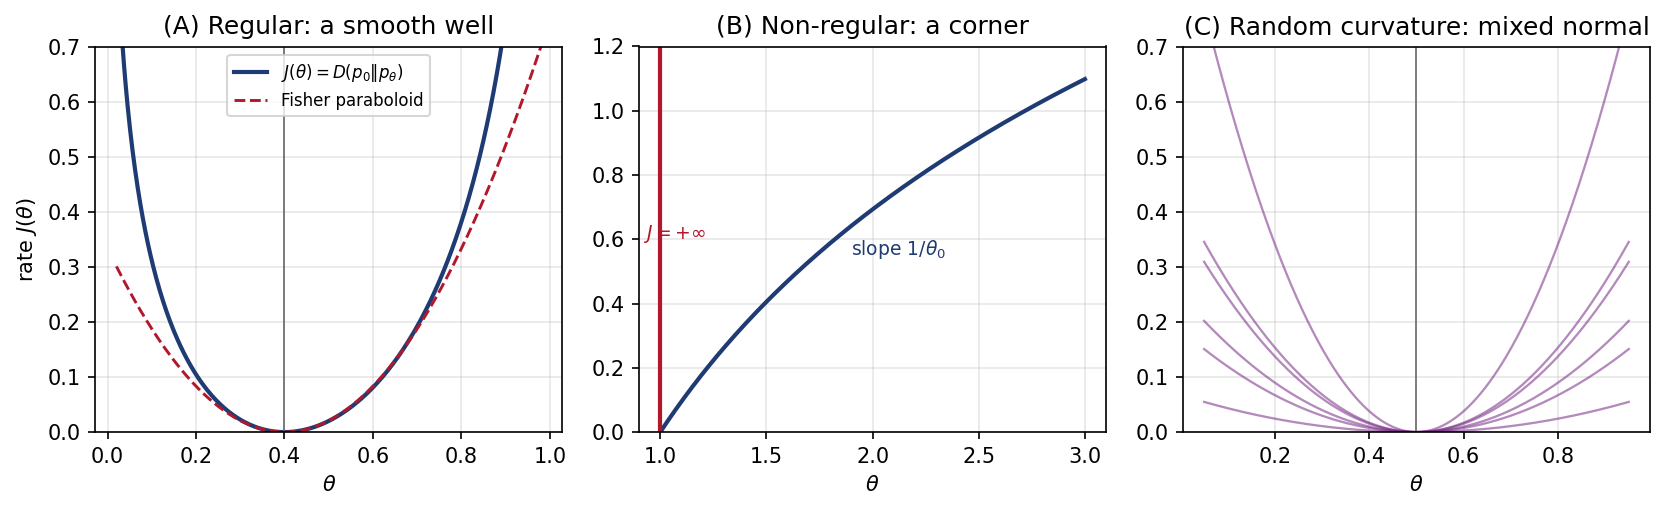
\includegraphics[width=\textwidth]{fig_bvm_regimes}
\caption{\small The three regimes as three shapes of the rate $J$ at the truth $\theta_0$.
(A) Regular (Beta--Bernoulli, $p_0=0.4$): a smooth well, locally the Fisher paraboloid (dashed),
whose exponential is a Gaussian posterior. (B) Non-regular (Uniform--Pareto, $\theta_0=1$): a corner,
an infinite wall on one side and finite slope $1/\theta_0$ on the other, whose exponential is an
exponential posterior contracting at rate $n$. (C) Random curvature (non-ergodic): a well whose
curvature $\eta^2$ is itself random, whose exponential is a mixed normal.}
\label{fig:regimes}
\end{figure}

\subsection{The regular case: the conjugate gallery}\label{sec:regular}
On the conjugate families every rung of the ladder is closed form, and the posterior is asymptotically Gaussian
because $J$ is a smooth well. For Beta--Bernoulli the posterior is $\mathrm{Beta}(\alpha+s,\beta+n-s)$,
the rate is $J(\theta)=\D{p_0}{\theta}$, and its curvature at $p_0$ is $1/\{p_0(1-p_0)\}$, the
Bernoulli Fisher information (Figure~\ref{fig:regimes}A). Dirichlet--Multinomial, Normal--Normal, and
Gamma--Poisson repeat the pattern: the posterior is the conjugate update, the rate is the
exponential-family divergence, and the Jeffreys prior is the square root of the curvature. Edgeworth corrections and probability-matching priors refine the inner, Bernstein--von Mises rung at higher order; the middle
rung, the moderate-deviation regime, has the prior-free Fisher quadratic as its rate; the outer rung is the full inverse-Sanov rate. Regularity and a
nondegenerate Hessian are two names for one condition, and, given posterior consistency and a prior positive and continuous at the truth, Bernstein--von Mises is its consequence.

\subsection{Non-regular problems: the rate has a corner}\label{sec:nonreg}
When the support of the model depends on the parameter and the density jumps at a moving edge of the support, quadratic-mean differentiability fails, the
Fisher information no longer measures the local curvature, and the rate has a corner rather than a bowl. The posterior then
contracts at rate $n$, not $\sqrt n$, and when a single edge moves, as in Example~\ref{ex:pareto}, its limit is exponential. A density that vanishes smoothly at a moving edge, such as a gamma location family with shape above $2$, can remain regular.

\begin{example}[Uniform--Pareto, in closed form]\label{ex:pareto}
Let $Y_i\sim \mathrm{Unif}(0,\theta)$ with prior $\theta\sim\mathrm{Pareto}(x_m,\alpha)$. Writing
$M_n=\max_i Y_i$, the likelihood is $\propto\theta^{-n}\mathbf 1\{\theta\ge M_n\}$, so the posterior
is again Pareto,
\[
\theta\mid Y_{1:n}\sim\mathrm{Pareto}\big(\max(x_m,M_n),\,n+\alpha\big),\qquad
n\Big(\frac{\theta}{M_n}-1\Big)\toL\mathrm{Exp}(1).
\]
The inverse-Sanov rate is $J(\theta)=\D{\mathrm{Unif}(0,\theta_0)}{\mathrm{Unif}(0,\theta)}=\log(\theta/\theta_0)$
for $\theta\ge\theta_0$ and $+\infty$ for $\theta<\theta_0$, because the truth is not absolutely
continuous with respect to a smaller uniform. This $J$ has a genuine corner at $\theta_0$: a vertical
wall on the left and a finite one-sided slope $J'(\theta_0^+)=1/\theta_0$ on the right, with no
quadratic piece, so the Fisher curvature is absent (Figure~\ref{fig:regimes}B). Its local shadow is
the exponential limit above: writing $\theta=\theta_0+s/n$ gives $nJ(\theta)\to s/\theta_0$,
so posterior mass decays like $e^{-nJ}=e^{-s/\theta_0}$ at rate $n$. Every clause of the non-regular
story (contraction rate $n$, exponential limiting posterior, absent Hessian) is a direct reading of
the cornered rate, and all of it is closed form.
\end{example}

The computational moral is that non-regular posteriors are read
from order statistics, not Gaussianized.

\subsection{Mixtures and the coexistence corner}\label{sec:mixture}
The interior corner is not exotic; it is the everyday consequence of a mixture prior, and it is where
every unimodal approximation fails.

\begin{example}[Two-component coexistence]\label{ex:coexist}
Let the data be exchangeable Bernoulli with a mixing measure
$\Pi=\tfrac12(\delta_a+\delta_b)$, $0<a<b<1$: with probability $\tfrac12$ the world is a coin-$a$
world, otherwise coin-$b$. By the Dinwoodie--Zabell large-deviation principle the empirical mean obeys
the \emph{non-convex} rate
\[
\lambda(x)=\min\{\D{x}{a},\D{x}{b}\},
\]
a double well vanishing at both $a$ and $b$ (Figure~\ref{fig:coexist}). The posterior over the world
label concentrates on whichever coin the data favor, and over the coexistence interval $(a,b)$ the
true rate is strictly positive while its convex envelope is flat at zero. A Gaussian, Laplace, or
mean-field variational posterior sees only the envelope: it fills the valley between the two wells and
reports intermediate means as unsurprising when they are in fact exponentially rare. For $a=0.25$,
$b=0.75$ the discarded rate at the midpoint is $\lambda(0.5)=0.144$ nats, the shaded gap in
Figure~\ref{fig:coexist}. The mixture corner is, in one picture, the failure of every unimodal
approximation.
\end{example}

\begin{figure}[H]
\centering
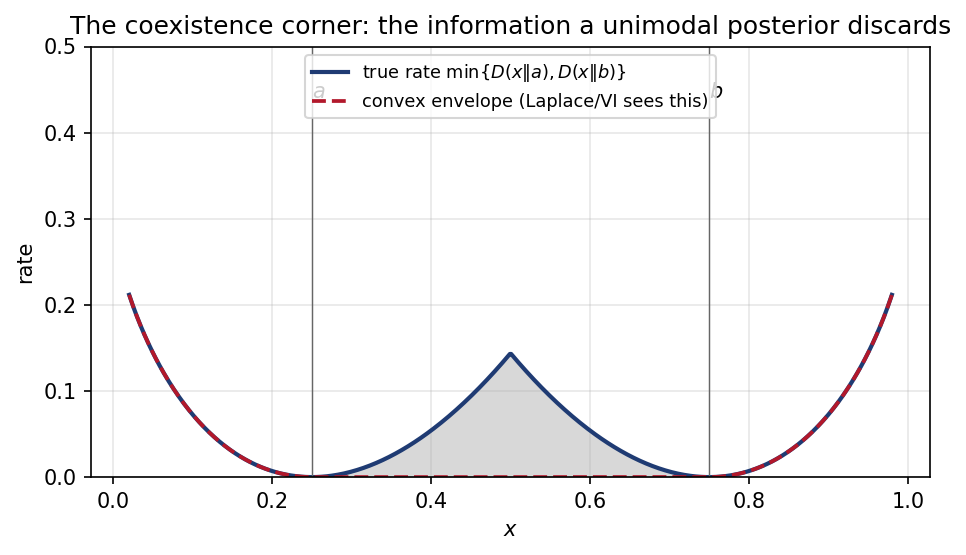
\includegraphics[width=0.72\textwidth]{fig_bvm_coexist}
\caption{\small The coexistence corner of Example~\ref{ex:coexist}. The true rate (solid) is the
non-convex double well $\min\{\D{x}{a},\D{x}{b}\}$; the convex envelope (dashed) that a Gaussian,
Laplace, or variational posterior returns is flat on $[a,b]$, so the shaded gap is the
information those approximations discard. The two wells are the two components; the corner between
them is where Bernstein--von Mises has nothing to say.}
\label{fig:coexist}
\end{figure}

The workhorse sparse prior, spike-and-slab $\theta\sim(1-w)\delta_0+w\,g(\theta)$, has the same
anatomy: a well at $0$, a well in the slab, and a corner between them at the coexistence threshold
where the marginal likelihoods of the two components cross. On one side the posterior loads the
spike, on the other the slab; near the threshold the two compete, and any unimodal posterior
convexifies the corner. This is why the horseshoe and other continuous global--local priors of
Sections~\ref{ch:hsmdp} and~\ref{ch:regular} are read through their heavy tails and origin behavior rather than through a Gaussian
approximation.

\subsection{Random curvature: non-ergodic processes and LAMN}\label{sec:lamn}
Non-ergodicity makes the curvature itself random. The observed information is a quadratic variation of
the score that does not converge to a constant but to a random limit, so the local quadratic bowl of
$J$ has a random second derivative: local asymptotic mixed normality (LAMN) in place of LAN. The
Sanov reading is the ergodic decomposition, which is the de Finetti mixing measure: conditionally on
the ergodic component the curvature is deterministic, and the mixture over components makes it random.

The cleanest illustration is a first-order autoregression $y_t=\theta y_{t-1}+\varepsilon_t$ read at
three values of $\theta$. Figure~\ref{fig:ar1} shows the sampling law of the least-squares estimator across the
three regimes from $4000$ simulated paths each, of length $n=200$ ($n=60$ in the explosive case). In the stationary case $\theta=0.5$,
$\sqrt n(\hat\theta-\theta)$ is Gaussian with variance $1-\theta^2=0.75$, matching the simulated
$0.774$: deterministic curvature. In the unit-root case $\theta=1$, $n(\hat\theta-\theta)$ is the
left-skewed Dickey--Fuller law (simulated skewness $-2.18$): boundary curvature. In the explosive case
$\theta=1.2$, $\theta^{n}(\hat\theta-\theta)$ is heavy-tailed and Cauchy-like: random curvature. The
\emph{estimator} leaves normality as the curvature becomes random, yet the conjugate-normal
\emph{posterior} stays Gaussian given the data, because it conditions on the realized observed
information rather than on its average. This is the Heyde--Johnstone phenomenon, that the posterior is
more robust than the estimator, and Polson and Roberts give it a decision-theoretic reading: the
curvature is the rate at which observing the path buys expected utility, and in the random-curvature
case that purchase is itself random, realized along the path rather than fixed in advance.

\begin{figure}[H]
\centering
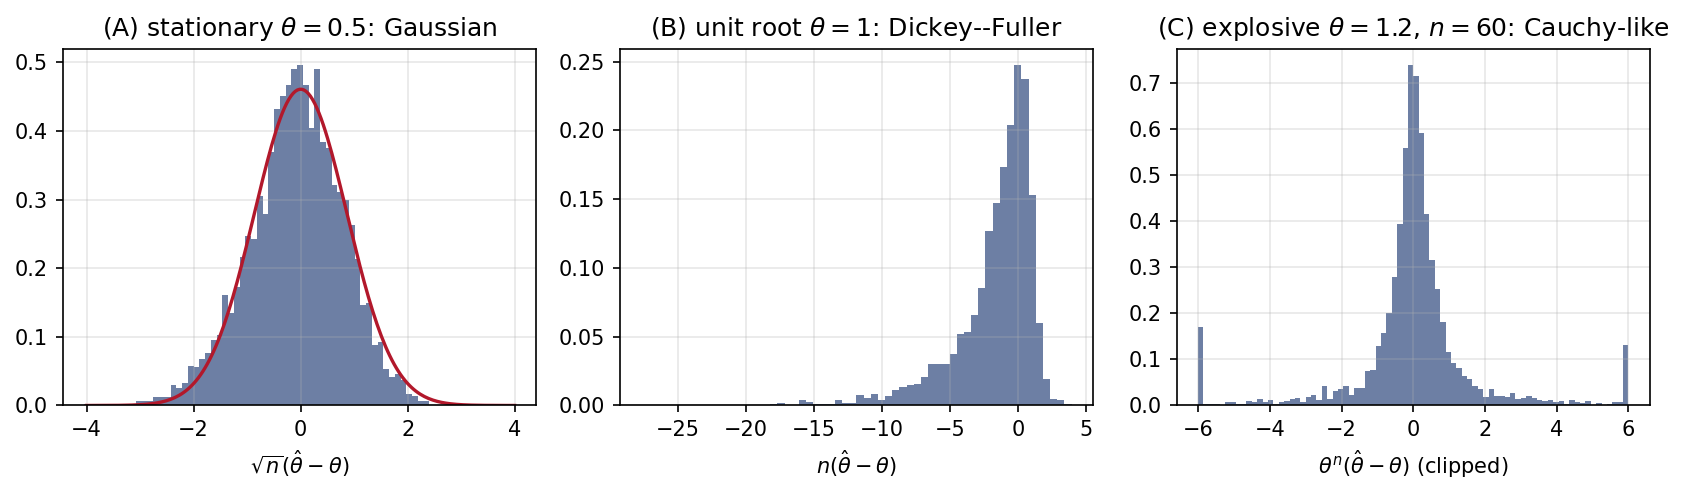
\includegraphics[width=\textwidth]{fig_bvm_ar1}
\caption{\small The Bayesian autoregression across three curvatures ($4000$ paths, $n=200$; $n=60$ in (C)).
(A) Stationary $\theta=0.5$: $\sqrt n(\hat\theta-\theta)$ is Gaussian, deterministic curvature.
(B) Unit root $\theta=1$: $n(\hat\theta-\theta)$ is the left-skewed Dickey--Fuller law, boundary
curvature. (C) Explosive $\theta=1.2$: $\theta^n(\hat\theta-\theta)$ has a heavy-tailed, random-curvature limit
(at large $n$ this statistic exhausts double precision, so it must be read at a moderate horizon).
The estimator leaves normality as the curvature becomes random, while the conjugate posterior stays
Gaussian given the data because it conditions on the realized information.}
\label{fig:ar1}
\end{figure}

\subsection{Misspecification: the minimum moves and the Hessian splits}\label{sec:misspec}
So far the truth was in the model. When it is not, the rate $\D{P_0}{\cdot}$ still has a minimum, but
the minimizer moves to the pseudo-true point, the reverse I-projection of the truth onto the model, and the
curvature splits into two matrices that regularity had forced to coincide.

\begin{proposition}[The split is the failure of the Bartlett identity]\label{prop:bartlett}
Let $\theta^\star$ be the pseudo-true parameter. The posterior (credible) precision is the model
curvature $V_\star=-\E_{P_0}\nabla^2\log p_{\theta^\star}$, while the sampling variance of the maximum
likelihood estimator is the sandwich $V_\star^{-1}\Sigma_\star V_\star^{-1}$ with
$\Sigma_\star=\mathrm{Var}_{P_0}\nabla\log p_{\theta^\star}$. When the model is correct the Bartlett
identity forces $V_\star=\Sigma_\star$ and the two coincide, so credible sets are confidence sets; under
misspecification they part company, and Bayesian credible intervals have the wrong width.
\end{proposition}

\begin{example}[$\N(\theta,1)$ fit to Student-$t_5$ data]\label{ex:sandwich}
Fit the location model $\N(\theta,1)$ to data that are actually Student-$t_5$ (variance $5/3$). The
pseudo-true point is $\theta^\star=0$, the model Fisher information is $V_\star=1$, so the posterior
sets its width by $V_\star^{-1}=1$; but the sampling law of $\hat\theta$ has the sandwich variance
$V_\star^{-1}\Sigma_\star V_\star^{-1}=5/3$. The $95\%$ credible band $[-1.96,1.96]/\sqrt n$ is therefore
too narrow by $\sqrt{5/3}\approx 1.29$ and covers only $87\%$ of the sampling distribution, as
Figure~\ref{fig:misspec} shows. The rate is still $\D{P_0}{\cdot}$; only its curvature and the score
covariance have parted company.
\end{example}

\begin{figure}[H]
\centering
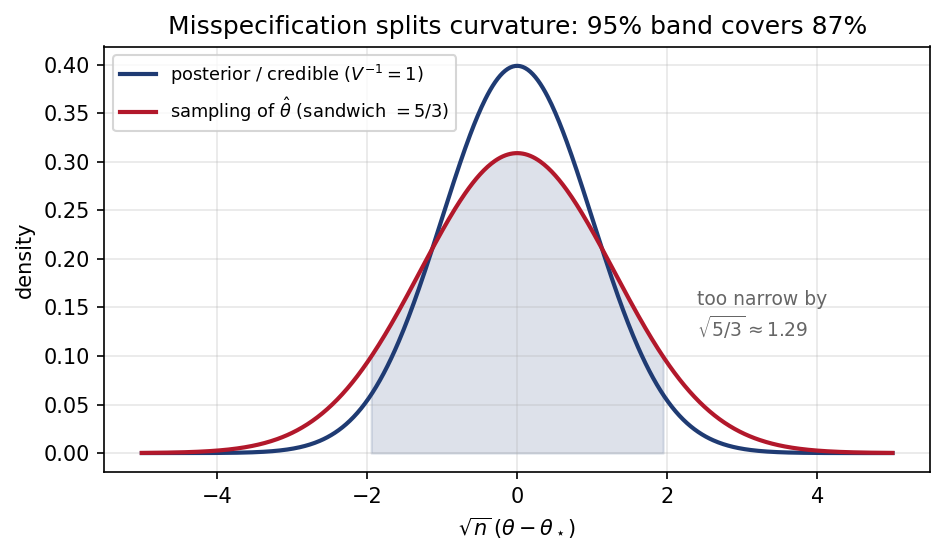
\includegraphics[width=0.72\textwidth]{fig_bvm_misspec}
\caption{\small Misspecification splits the curvature (Example~\ref{ex:sandwich}). The posterior /
credible law (taller curve, variance $V_\star^{-1}=1$) is narrower than the sampling law of $\hat\theta$ (wider curve,
sandwich variance $5/3$). The $95\%$ credible band covers about $87\%$; it is too narrow by
$\sqrt{5/3}\approx1.29$. When the model is correct the Bartlett identity makes the two coincide.}
\label{fig:misspec}
\end{figure}

Three honest responses address the failure of the identity $V_\star=\Sigma_\star$ that regularity gave for free. Report
the sandwich, following the robust-variance correction (White, 1982; M\"uller, 2013). Temper the likelihood, as in the Gibbs
posteriors (Bissiri, Holmes and Walker, 2016) and safe-Bayes learning rate (Gr\"unwald and van Ommen, 2017), rescaling until the reported curvature matches the
information the data carry. Or resample, as in the loss-likelihood (Lyddon, Holmes and Walker, 2019) and weighted-Bayesian (Newton, Polson and Xu, 2021) bootstraps,
replacing one misspecified posterior by a distribution over pseudo-true points whose spread is the
sandwich. The first corrects the report, the second the temperature, the third the sampling.

\subsection{Infinite dimensions: the curvature becomes an operator}\label{sec:infinite}
The last degeneracy is dimension. In a nonparametric model the parameter is a function and the
curvature of the rate is an operator, the information operator, whose inverse is typically
not trace class (for the Gaussian white-noise model the operator is the identity). The Gaussian shadow of the rate then lives, if at
all, only in a weak topology, and the strong Bernstein--von Mises statement fails. The failure is
generic: for the Gaussian white-noise or sequence model, credible sets can cover the truth with
probability tending to zero, because the posterior spread and the frequentist sampling error differ by
a random offset the credible set does not see. What survives is a weak-topology Bernstein--von Mises
theorem for smooth functionals, and the Dirichlet-process exception, where the posterior for the
distribution function is asymptotically a Gaussian process. The lesson is the same as the finite
degeneracies, one level up: a Gaussian whose covariance is the inverse curvature of the
rate is a probability measure on the parameter space only when that inverse is trace class, which is
automatic in finite dimensions and in infinite dimensions typically holds only in a weaker topology.

\paragraph{Summary.}
Bernstein--von Mises is the curvature of the inverse-Sanov rate, exponentiated
(Proposition~\ref{prop:reg}), and in finite dimensions, given posterior consistency and a prior positive and continuous at the truth, it holds when that curvature is finite, fixed, and positive
definite. The five classical failures are the five ways the curvature degenerates: it \emph{is
absent}, leaving a corner, when the model is non-regular (Section~\ref{sec:nonreg}); it \emph{splits into two
wells} when the prior is a mixture (Section~\ref{sec:mixture}); it \emph{becomes random} when the
process is non-ergodic (Section~\ref{sec:lamn}); it \emph{splits into two matrices} when the model is
misspecified (Section~\ref{sec:misspec}); and it \emph{becomes an operator whose inverse is not trace class} in infinite
dimensions (Section~\ref{sec:infinite}). Regular Bayes, non-regular Bayes, mixture Bayes, non-ergodic
Bayes, misspecified Bayes, and nonparametric Bayes are then one statement about the curvature of a
rate function: fixed, absent, doubled, random, split, or with an inverse of infinite trace.

\subsection*{Problems}
\begin{enumerate}[leftmargin=2.2em,itemsep=2pt]
\item Prove Proposition~\ref{prop:reg} for a one parameter exponential family: the posterior is
asymptotically Gaussian if and only if the rate function has a positive second derivative at its
minimum, and the variance is the reciprocal of that curvature over $n$.
\item In Example~\ref{ex:pareto}, derive the limit law of the posterior on the scale $n^{-1}$ and show
that the rate function is linear, not quadratic, on one side of its minimum.
\item For the two component example, show that the posterior odds between the components decay
exponentially at a rate equal to a difference of divergences, and find where the rate has a corner.
\item For a Gaussian AR(1) with coefficient one, show that the observed information divided by $n^2$
converges to a random limit, and that the posterior is asymptotically a scale mixture of normals.
\item In Example~\ref{ex:sandwich}, compute the sandwich variance of the posterior mean and the ratio
to the posterior variance, and relate it to the failure of the Bartlett identity in
Proposition~\ref{prop:bartlett}.
\item In the Gaussian sequence model with a Gaussian prior, write the curvature operator and show that
its inverse is unbounded, so that the Bernstein and von Mises theorem fails in the strong norm.
\end{enumerate}

\src{When Is Bayes Gaussian? (2026e); the inverse-Sanov representation of Section~\ref{ch:inverse}; Ganesh and O'Connell
(1999, 2000); Eichelsbacher and Ganesh (2002a); Ghosh, Ghosal, and Samanta on non-regular posteriors;
Dinwoodie and Zabell on mixture large deviations; Heyde and Johnstone (1979) and Polson and Roberts
(1993) on random curvature; Kleijn and van der Vaart (2012) on misspecified Bernstein--von Mises; and
Cox (1993), Freedman (1999), and Castillo and Nickl (2013) on the infinite-dimensional case.}

%====================================================================================================

%====================================================================================================



\chapter{Scalable Computation and Deep Learning}\label{chap:computation}

A predictive theory is only as useful as the algorithms that realize it. This chapter turns the
synthesis into computation. Data augmentation introduces latent variables that make an intractable
likelihood conditionally conjugate, and the P\'olya--Gamma scheme does this for the entire logistic and
multinomial family. Proximal and optimization-based methods reveal estimation and sampling as two
readings of one iteration, and deep learning appears as hierarchical predictive regression whose
regularization is codelength rather than parameter count.
Entropy-regularized prediction derives the information cost of a forecast from proper scoring and shows that the risk--complexity frontier is a rate--distortion curve; generative Bayesian prediction delivers a posterior as a trained sampler rather than a density; and double descent, with ordered empirical Bayes, shows that past the interpolation threshold what saturates is the effective complexity the evidence pays for.

The unifying message is that the maximum-entropy, exponential-tilt form of the synthesis is
what makes modern computation tractable: augmentation restores conjugacy, gradient flow follows the
score, and variational bounds are two-part codes. The algorithms are not a grab-bag but consequences of
the predictive geometry.


\section{Entropy-Regularized Prediction and Rate--Distortion}\label{ch:er}

\noindent\textbf{Thesis.} Three axioms on how predictions are scored, locality, strict propriety, and
coherence under aggregation, single out the log score and, with it, Shannon mutual information as the
measure of predictive complexity. The resulting risk--complexity frontier is a rate--distortion
curve, and Blahut--Arimoto is its solver. This is Cover and Thomas's Chapter~10 read as a predictive
decision problem, with the information cost derived rather than imposed.

\subsection{Predictive rules and the characterization of the log score}
Treat an inferential object as a \emph{predictive rule}: a mapping from information to a reported
predictive distribution over outcomes. Impose three structural requirements on how such a rule is
evaluated. \emph{Locality}: the score at an outcome depends only on the probability the rule assigned
to that outcome. \emph{Strict propriety}: the rule's expected score is maximized by reporting its
true predictive law. \emph{Coherence under aggregation}: coarsening or refining the outcome
categories does not change the ranking of rules (amalgamation invariance).

\begin{theorem}[Characterization]\label{thm:logscore}
A predictive evaluation on at least three outcomes satisfying locality, strict propriety, and coherence under aggregation is, up
to an affine transformation, the logarithmic score $S(p,x)=\log p(x)$. The induced measure of
predictive complexity is Shannon mutual information, equivalently the Kullback--Leibler divergence of
the predictive law from its baseline.
\end{theorem}

\begin{proof}[Proof sketch]
We sketch the differentiable case (Bernardo, 1979a). Locality makes the score $S(p,x)=u(p(x))$ for one function $u$, and strict propriety makes $q=p$ the maximizer of $\sum_x p(x)\,u(q(x))$ subject to $\sum_x q(x)=1$, so $p(x)\,u'(p(x))=\lambda(p)$ for every outcome $x$ with $p(x)>0$. With at least three outcomes any two laws in the interior of the simplex are joined by a third that agrees with the first at one outcome and with the second at another, so $\lambda$ is a constant, $u'(t)=\lambda/t$, and $u(t)=\lambda\log t+c$ with $\lambda>0$. With two outcomes the Brier score also depends only on $p(x)$, which is why three are needed; the third axiom is not used. The expected regret of reporting $q$ when $p$ is true is then $\D{p}{q}$, as computed below, and its average over the information, with $q$ the marginal predictive law, is the mutual information between the information and the outcome.
\end{proof}

The content of Theorem~\ref{thm:logscore} is that complexity need not be assumed. Once one accepts
that predictions are scored locally, honestly, and consistently across levels of description, the log
score and mutual information are forced, as in Section~\ref{ch:predictive} coherence forced
the Bayesian representation. Relative entropy reappears here not as a coding length but as expected
predictive regret, which is the reading used throughout the book.

\subsection{Proper scoring rules and Bregman divergences}
A forecast is judged by a scoring rule $S(q,y)$ that rewards a report $q$ when $y$ occurs, and the rule
is \emph{proper} when honesty pays, meaning $\E_{y\sim p}S(q,y)$ is maximized at $q=p$, and
\emph{strictly proper} when that maximizer is unique. Propriety is the condition that a
forecaster paid by the rule has no incentive to misreport, so it is the operational face of coherence.
Among all strictly proper rules the logarithmic score $S(q,y)=\log q(y)$ is singled out twice over: it
is the only \emph{local} score (given at least three outcomes), depending on the report only through the probability $q(y)$ it placed on
the outcome that occurred, and it is the only score whose running total is a codelength. This is the
first advantage of reading Bayes through information theory. The quantity a coherent forecaster is
scored by is forced, up to affine choices, to be the log score, and the log score is measured in nats.

Every proper score carries an information geometry. Write $G(p)=\E_p S(p,\cdot)$ for the greatest
expected reward available to a forecaster who believes $p$, a convex function of $p$. The Savage
representation reconstructs the score from this one function as $S(q,y)=G(q)+\langle\nabla
G(q),\,e_y-q\rangle$, and the regret for reporting $q$ instead of the truth $p$,
\[
d(p,q)=\E_p S(p,\cdot)-\E_p S(q,\cdot)=G(p)-G(q)-\langle\nabla G(q),\,p-q\rangle,
\]
is the Bregman divergence generated by $G$. The choice of score is the choice of $G$. Taking
$G=-H$, the negative Shannon entropy, gives the log score and makes the regret the Kullback--Leibler
divergence $\D{p}{q}$; taking $G(p)=\lVert p\rVert^2-1$ gives the Brier score and makes the regret
squared error; the continuous ranked probability score is the distributional member of the same family.
So the divergence the book has used to price evidence, to run Sanov's theorem, and to measure predictive
contraction is not an arbitrary choice. It is the honesty penalty of the one local proper score, and
every other proper score simply names a different Bregman geometry on the simplex. Elicitability, the
question of whether a functional is the minimizer of some expected score, follows the same
convex-analytic pattern: the mean, quantiles, and expectiles are elicitable, while the variance alone is
not.

\subsection*{Worked example: the honesty penalty is relative entropy}
Let the truth be a coin with heads probability $p$ and let a forecaster report $q$. The expected log
score is $p\log q+(1-p)\log(1-q)$, maximized at $q=p$ with value $-H(p)$, so a forecaster who reports
$q\neq p$ loses exactly
\[
p\log\frac{p}{q}+(1-p)\log\frac{1-p}{1-q}=\D{p}{q}
\]
nats on each forecast. The penalty for being wrong is the relative entropy from the truth to the report,
and summing it along a data sequence is the excess codelength the forecaster pays over an oracle who
knows $p$, the same per-parameter $\tfrac12\log n$ that BIC charges once $q$ is a fitted model. Reporting
the Bayes posterior predictive minimizes this penalty in expectation, which is the information-theoretic
statement that the predictive is the best-calibrated forecast the data allow. The advantage of the view
is concreteness: coherence, calibration, and compression are here one inequality, not three separate
virtues.

\subsection{Calibration, sharpness, and the Murphy decomposition}
A stream of probability forecasts is \emph{calibrated} when events it calls probability $p$ occur a
fraction $p$ of the time, and \emph{sharp} when those forecasts are as decisive as calibration allows.
The two are not rivals: sharpness is what a forecaster should maximize subject to remaining calibrated.
Scoring the stream audits both at once. The expected negative log score of a forecast sequence splits, in
Murphy's decomposition, as uncertainty minus resolution plus reliability, where uncertainty is the
base-rate entropy the world imposes, resolution rewards forecasts that separate the outcomes, and
reliability penalizes miscalibration by a relative entropy between stated and realized frequencies. A
perfectly calibrated forecaster carries a zero reliability term and is scored purely on the uncertainty
it resolved, so the single currency of nats pays for sharpness and fines miscalibration together. The
running total of the score is the prequential codelength of Section~\ref{ch:evalues}, so calibration,
sharpness, and compression are three readings of one number. This is the second advantage of the
information-theoretic view. Model criticism, which in the parameter-first picture needs a separate
apparatus of tests, becomes the bookkeeping of a codelength, and a reliability diagram is a picture of
the excess nats a miscalibrated forecaster spends. When calibration fails it can be repaired after the
fact by an isotonic or Platt recalibration (Platt, 2000), a monotone map. Platt's logistic map leaves the ranking, and with it the resolution, intact and removes
the reliability penalty when the miscalibration is logistic; an isotonic fit removes the penalty on the fitting sample but pools forecast values, which can lower the resolution.


\subsection{The risk--complexity frontier is a rate--distortion curve}
Let a rule report the conditional law $q(y\mid x)$ of an action or forecast $y$ given a state $x$
with prior $p(x)$, evaluated by an expected loss (distortion) $\E[d]$ and penalized by its mutual
information $I(X;Y)$ at price $\lambda^{-1}$ per nat. The entropy-regularized prediction problem is
\begin{equation}\label{eq:rd}
\min_{q}\ I(X;Y)+\lambda\,\E[d],
\end{equation}
and its solution is the Gibbs rule $q^\star(y\mid x)\propto \bar q^\star(y)\,e^{\lambda\,U(x,y)}$ with
$U=-d$ and $\bar q^\star$ the induced marginal. The optimal value traces, as $\lambda$ varies, a
frontier in the plane of complexity against risk.

\begin{proposition}[The frontier is $R(D)$]\label{prop:rd}
The set of $(I(X;Y),\E[d])$ pairs attained by \eqref{eq:rd} is the rate--distortion curve $R(D)$:
convex and non-increasing, with slope $-\lambda$ at each point. Calibrating a rule to an information
budget $\kappa$ is the single equation $I(q^\star_\lambda)=\kappa$, one $R(D)$ evaluation plus a
monotone one-dimensional root find.
\end{proposition}

\begin{proof}[Proof sketch]
The function $R(D)=\min\{I(X;Y):\E[d]\le D\}$ is non-increasing because the constraint relaxes as $D$ grows, and convex because $I(X;Y)$ is convex in the channel while $\E[d]$ is linear in it (Cover and Thomas, 2006, Chapter~10). If $q^\star_\lambda$ solves \eqref{eq:rd} with distortion $D_\lambda$, no channel with distortion at most $D_\lambda$ carries less information, so $I(q^\star_\lambda)=R(D_\lambda)$, and $R(D)+\lambda D\ge R(D_\lambda)+\lambda D_\lambda$ for every $D$: the line of slope $-\lambda$ through $(D_\lambda,R(D_\lambda))$ supports the curve there. Comparing the optimality of $q^\star_\lambda$ and $q^\star_{\lambda'}$ at both prices shows that the distortion falls and $I(q^\star_\lambda)$ rises as $\lambda$ grows, which makes the budget equation a monotone root find.
\end{proof}

This is the point of contact with Cover and Thomas. Their rate--distortion function is the least
mutual information a channel needs to meet a distortion budget; here the same curve is the least
predictive complexity a rule needs to meet a risk budget, and the Lagrange multiplier $\lambda$ is
not a tuning constant but the shadow price of risk, in nats per risk unit, and minus the slope of
the frontier.

\subsection{Blahut--Arimoto as the solver}
The problem \eqref{eq:rd} is solved by the same alternating minimization that computes the I-projections
of Section~\ref{ch:maxent}, once one identifies mutual information as already a minimum.

By Lemma~\ref{lem:me-marginal} of Section~\ref{ch:maxent}, $I(X;Y)=\min_m \sum_x p(x)\,\D{q(\cdot\mid x)}{m}$, attained uniquely at the induced marginal $m^\star(y)=\sum_x p(x)\,q(y\mid x)$, so the rate--distortion problem is a joint minimization over channels and
marginals, each step a closed-form I-projection: the $q$-step is the Gibbs tilt of
Theorem~\ref{thm:vcc}, the $m$-step is the marginal update. Alternating them is Blahut--Arimoto,
monotone and step-size free by the Csisz\'ar--Tusn\'ady five-point property. Two canonical cases
recur. In the linear--quadratic Gaussian case the solution is \emph{reverse water-filling}: capacity
is spent on the high-variance directions and directions below the water level receive exactly zero
nats, so finite capacity ignores most of the state entirely rather than blurring all of it. In the
discrete-choice case the fixed point is a multinomial logit with an endogenous prior, and low-appeal
options leave the consideration set at exact zeros of the marginal, an active-set phenomenon of
complementary slackness, as in the inequality-constrained I-projection.

\subsection{Rational inattention, and specializations}
The self-consistent baseline is Sims's rational inattention: an agent conditions actions on a
state only through a channel of finite Shannon capacity, choosing the joint law to maximize expected
payoff subject to $I(\omega;a)\le\kappa$. That capacity constraint is a rate--distortion constraint,
so Blahut--Arimoto is its solver, a fact the economics literature has repeatedly rediscovered without
naming. Canonical models are geometric specializations of the one Gibbs--Boltzmann channel:
multinomial logit and the independence of irrelevant alternatives under entropic regularization;
James\index{James--Stein estimator}--Stein shrinkage as optimal capacity allocation in a Gaussian learning problem; and
linear-quadratic-Gaussian control as the capacity-optimal Gaussian channel. An essentially
complete-class theorem holds: the admissible rules under joint risk--complexity dominance are the
Gibbs rules, up to the boundary cases $\lambda=0$ and $\lambda=\infty$. Mutual information is convex in the rule and expected loss is linear, so the (complexity, risk) pairs that some rule matches or beats in both coordinates form a convex set. An admissible rule lies on its boundary, where a supporting line makes it a minimizer of \eqref{eq:rd} for some $\lambda\in[0,\infty]$ (at $\lambda=\infty$, of $\E[d]$ alone); conversely a minimizer with $0<\lambda<\infty$ is admissible, since a rule dominating it would lower $I(X;Y)+\lambda\,\E[d]$.

\begin{remark}
The derivation runs opposite to Cover and Thomas. They fix a distortion budget and ask for the least rate; here
the information cost is derived from proper scoring (Theorem~\ref{thm:logscore}) and then the optimal
channel is computed. Shannon entropy is endogenous, the honest local utility for predictive
refinement, rather than a constraint imposed from outside. This is why the section belongs to a
Bayesian theory of prediction and not only to information theory.
\end{remark}



\subsection*{Worked example: the Gibbs law as entropy-regularized choice}
This example shows that penalizing an expected loss by relative entropy produces the exponential tilt, with a temperature that dials between decisiveness and hedging.

Minimize $\E_q[L]+T\D{q}{\pi}$ over $q$ on a finite set with $\pi$ uniform and losses $L_k$. The optimum is the Gibbs law $q_k\propto e^{-L_k/T}$, and the optimal value is $-T\log\!\big(\tfrac1K\sum_k e^{-L_k/T}\big)$, a soft-min that tends to $\min_k L_k$ as $T\to0$ and to the uniform average as $T\to\infty$. The temperature $T$ interpolates between exploitation and exploration.

The soft-min value $-T\log\!\big(\tfrac1K\sum_k e^{-L_k/T}\big)$ is the free energy of the problem, and its limits are the two regimes of every entropy-regularized method here: as $T\to0$ it becomes the hard minimum and commits to the best action, while as $T\to\infty$ it becomes the prior mean and explores uniformly. Bandits, reinforcement learning, and rate--distortion all reuse this identity.

\paragraph{Summary.}
Entropy-regularized prediction adds a Kullback--Leibler penalty to a scoring objective, and the optimum is a Gibbs distribution; the rate--distortion function is the same variational problem read as a tradeoff between compression and fidelity. The temperature is the Lagrange multiplier on the entropy constraint.

\subsection*{Problems}
\begin{enumerate}[leftmargin=2.2em,itemsep=2pt]
\item Show that minimizing expected loss plus $T\D{q}{\pi}$ over $q$ yields the Gibbs form $q\propto\pi\,e^{-L/T}$.
\item Derive the rate--distortion function of a Gaussian source under squared-error distortion.
\item Interpret the temperature $T$, the reciprocal of $\lambda$ in \eqref{eq:rd}, as a Lagrange multiplier and describe the $T\to0$ and $T\to\infty$ limits.
\item Connect the Gibbs optimum to the maximum-entropy exponential family of Section~\ref{ch:maxent}.
\item Show the free-energy objective is convex in $q$ and identify its minimum value as a log-partition function.
\end{enumerate}

\src{Entropy-Regularized Inference (2512.21639); Maximum Entropy Algorithms for Predictive Rules
(2026d).}

%====================================================================================================

\shorthead{Data Augmentation and Scale Mixtures}
\section{Data Augmentation, Scale Mixtures, and Latent-Variable Bayes}\label{ch:augment}

\noindent\textbf{Thesis.} Almost every hard Bayesian computation becomes easy once
the right latent variable is introduced. A likelihood that is awkward on its own is
very often a mixture, a marginal of a conditionally conjugate model over a hidden
scale or a hidden P\'olya--Gamma variate, and the mixing representation converts an
intractable posterior into a Gibbs sampler that alternates between complete
conditionals in closed form. This section collects the data-augmentation identities
that run underneath the rest of the book: the normal variance-mean mixture that
turns non-Gaussian regression into weighted least squares, the P\'olya--Gamma
mixture that turns logistic and negative-binomial likelihoods conditionally
Gaussian, and the global-local scale mixture that makes the horseshoe a
one-line hierarchical model. The unifying fact is the one already used for the EM
and shrinkage sections: a marginal is a mixture, and the mixing variable is the
computational handle.

\subsection{The augmentation principle}\label{da:sec:principle}

Let the target posterior be $p(\theta\mid y)\propto \pi(\theta)\,f(y\mid\theta)$ with
$f$ awkward, not conjugate, not log-concave in a convenient variable, or simply
without a closed-form normalizer. Data augmentation introduces a latent
$\omega$ with a joint $p(\theta,\omega\mid y)$ whose marginal in $\theta$ recovers
the target,
\[
\int p(\theta,\omega\mid y)\,d\omega \;=\; p(\theta\mid y),
\]
and whose two complete conditionals $p(\theta\mid\omega,y)$ and
$p(\omega\mid\theta,y)$ are both tractable. The Gibbs sampler that alternates them
has $p(\theta\mid y)$ as its $\theta$-marginal stationary law, so draws of $\theta$
are exact posterior draws once the chain mixes. The art is entirely in the choice of
$\omega$: it should be a variable in terms of which the likelihood is conditionally
conjugate. Three constructions cover most of the models in this book.

\subsection{Normal variance-mean mixtures}\label{da:sec:vmm}

A density $f$ is a \emph{normal variance-mean mixture} if
\[
f(y)=\int_0^\infty \N\!\big(y \mid \mu+\beta\,\omega,\;\omega\big)\,g(\omega)\,d\omega
\]
for a mixing law $g$ on $(0,\infty)$. Conditional on $\omega$ the observation is
Gaussian, so a regression likelihood built from such errors is, given the vector of
$\omega_i$, an ordinary weighted least-squares problem: the complete conditional for
the coefficients is Gaussian with precision $X^\top \mathrm{diag}(1/\omega_i)X$ plus
the prior precision. The mixing law $g$ selects the error shape. Taking $g$ exponential (Andrews and Mallows, 1974) gives a
symmetric Laplace (double-exponential) marginal and hence the Bayesian lasso\index{Bayesian lasso};
taking $g$ a positive stable law gives the bridge densities below; taking $g$ an
exponential in a location-scale mixture gives the asymmetric-Laplace likelihood of Bayesian quantile regression.
The same device drives regularized regression: a penalty $\mathrm{pen}(\theta)$ that
can be written as the negative log of a scale mixture of normals,
$e^{-\mathrm{pen}(\theta)}=\int \N(\theta\mid0,\tau^2)\,h(\tau^2)\,d\tau^2$, is
handled by augmenting with $\tau^2$ and running the Gaussian complete conditional;
this is the representation that put the EM and shrinkage estimators of
Sections~\ref{ch:maxent} and~\ref{ch:hsmdp} on a common footing.

\subsection{P\'olya--Gamma augmentation for binomial likelihoods}\label{da:sec:pg}

Logistic and negative-binomial likelihoods resisted a clean Gaussian augmentation
for two decades. The obstruction is the logistic normalizer: a binomial likelihood
in the log-odds $\psi=x^\top\beta$ carries a factor $(1+e^\psi)^{-b}$ that is not a
Gaussian kernel in $\beta$. The P\'olya--Gamma family removes it. A random variable
$\omega$ has a \emph{P\'olya--Gamma} law $\mathrm{PG}(b,c)$ if it is an infinite
convolution of gammas,
\[
\omega \;\eqdist\; \frac{1}{2\pi^2}\sum_{k=1}^\infty
\frac{g_k}{(k-\tfrac12)^2+c^2/(4\pi^2)},\qquad g_k\iid\mathrm{Gamma}(b,1).
\]
Its role is captured by a single integral identity: for $b>0$,
\[
\frac{(e^\psi)^{a}}{(1+e^\psi)^{b}}
\;=\;2^{-b}e^{\kappa\psi}\!\int_0^\infty e^{-\omega\psi^2/2}\,p(\omega)\,d\omega,
\qquad \kappa=a-b/2,\;\; \omega\sim\mathrm{PG}(b,0).
\]
Read as a statement about the likelihood, it says that a binomial likelihood is a
Gaussian in $\psi$ once mixed over a P\'olya--Gamma scale. The consequences are
immediate. Conditional on $\omega_i$, the logistic regression likelihood is
proportional to $\exp\{-\tfrac12\sum_i\omega_i(z_i-x_i^\top\beta)^2\}$ with working
responses $z_i=\kappa_i/\omega_i$, so the complete conditional for $\beta$ is exactly
Gaussian, $\beta\mid\omega,y\sim\N(m_\omega,V_\omega)$ with
$V_\omega=(X^\top\Omega X+B_0^{-1})^{-1}$ and $\Omega=\mathrm{diag}(\omega_i)$; and
the complete conditional for each latent is again P\'olya--Gamma,
$\omega_i\mid\beta\sim\mathrm{PG}(b_i,x_i^\top\beta)$, for which an exact,
tuning-free sampler exists. The awkward GLM posterior becomes a two-block Gibbs
sampler of Gaussian and P\'olya--Gamma draws.

\begin{theorem}[P\'olya--Gamma Gibbs for binomial models]\label{da:thm:pg}
For a binomial likelihood with logit $\psi_i=x_i^\top\beta$ and any Gaussian prior
$\beta\sim\N(b_0,B_0)$, the augmented chain with steps
$\omega_i\mid\beta\sim\mathrm{PG}(n_i,x_i^\top\beta)$ and
$\beta\mid\omega,y\sim\N(m_\omega,V_\omega)$, $V_\omega=(X^\top\Omega X+B_0^{-1})^{-1}$,
$m_\omega=V_\omega(X^\top\kappa+B_0^{-1}b_0)$, $\kappa_i=y_i-n_i/2$ for $y_i$ successes in $n_i$ trials, has the exact posterior
$p(\beta\mid y)$ as its $\beta$-marginal stationary distribution, and the sampler is
uniformly ergodic.
\end{theorem}

Choi and Hobert (2013) prove the uniform ergodicity for binary responses. A count of $y_i$ successes in $n_i$ trials is $n_i$ binary rows sharing $x_i$. The $\beta$-step uses those rows only through the sum of their $\kappa$'s, which is $y_i-n_i/2$, and the sum of their latents, which is $\mathrm{PG}(n_i,x_i^\top\beta)$ because independent P\'olya--Gamma variates with a common $c$ add in $b$. The $\beta$-chain of the binomial sampler is therefore that of the binary rows, and the result carries over.

The construction extends verbatim to negative-binomial regression (count data with
overdispersion), to multinomial logit through the
one-versus-rest representation, to nonlinear mixed models, and to spatial models for
count data. Because every step is conjugate, the same augmentation powers the
mean-field and structured variational approximations of Section~\ref{ch:vi}:
the P\'olya--Gamma expectation $\E[\omega\mid\beta]=\tfrac{b}{2c}\tanh(c/2)$ is
available in closed form, so the variational updates need no quadrature. A companion
construction, the P\'olya-inverse-Gamma family, extends the same idea to gamma,
inverse-gamma, beta, and Dirichlet likelihoods by writing the reciprocal gamma
function as a scale mixture of normals, which brings Dirichlet allocation models
into the same conditionally Gaussian scheme.

\subsection{The Bayesian bridge and global-local shrinkage}\label{da:sec:bridge}

Bridge regression penalizes $\sum_j|\beta_j|^\alpha$ for $0<\alpha\le2$, interpolating
between ridge ($\alpha=2$) and best-subset ($\alpha\to0$) and giving sparser fits
than the lasso for $\alpha<1$, where the penalty is nonconvex and the prior tails are stretched exponential. The penalty is not obviously a mixture, yet
$\exp(-|\beta_j|^\alpha)$ is a scale mixture of normals with an
$\alpha/2$-stable mixing law. Augmenting with those stable scales turns the bridge
posterior into a Gaussian complete conditional for $\beta$ and a tilted stable draw for the
scales, the same variance-mixture machinery of \S\ref{da:sec:vmm}. This is the
computational face of the global-local view of shrinkage: write
$\beta_j\mid\lambda_j,\tau\sim\N(0,\lambda_j^2\tau^2)$ with local scales $\lambda_j$
and a global scale $\tau$, and different priors on $\lambda_j$ reproduce the whole
zoo, exponential scales give the lasso, stable scales give the bridge, and a
half-Cauchy on $\lambda_j$ gives the horseshoe of Section~\ref{ch:hsmdp}. The
half-Cauchy is not arbitrary: it is the prior whose global-scale calibration is
robust, and it is the boundary case at which the marginal prior on $\beta_j$ acquires
both an infinite spike at the origin (to shrink noise) and Cauchy-heavy tails (to
leave signals unshrunk), the two defining properties of a good sparsity prior. Local
shrinkage rules of this form are, in the continuous limit, the L\'evy
processes whose increments furnish the mixing measure, which is why the shrinkage
profile and the prior tail are two readings of one L\'evy density.

\subsection{Data augmentation for classifiers and the wider pattern}\label{da:sec:wider}

The same principle reaches beyond likelihoods with a natural mixture form. The
support-vector-machine hinge loss, which is not a likelihood at all, can be given a
pseudo-likelihood that is a location-scale mixture of normals, so Bayesian SVM
classification runs as a conditionally Gaussian Gibbs sampler and returns full
posterior uncertainty on the separating hyperplane, not just a point estimate.
Simulation-based regularized logistic regression uses the same latent-variable route
to trace the whole regularization path as a posterior rather than by repeated
optimization. In each case the pattern is identical to the augmentation principle of
\S\ref{da:sec:principle}: locate the hidden variable in terms of which the model is
conjugate, and the intractable object dissolves into a loop of closed-form draws.
Read against the information-theoretic spine of this book, augmentation is the
computational dual of the mixture-is-a-marginal identity: where the coding and
evidence sections integrate the latent out to price a model, the sampler holds the
latent in to explore the posterior, and the same conditional-conjugacy that makes
the integral clean makes the draw closed-form.


\subsection{A worked example: the P\'olya--Gamma logistic sampler}\label{da:sec:worked}

To make the mechanics concrete, take logistic regression with $n$ observations
$y_i\in\{0,1\}$, covariates $x_i\in\R^p$, logit $\psi_i=x_i^\top\beta$, and prior
$\beta\sim\N(0,B_0)$. Each sweep of the sampler has two steps. First, given
$\beta$, draw the latents $\omega_i\sim\mathrm{PG}(1,x_i^\top\beta)$ independently;
the P\'olya--Gamma sampler does this exactly, without tuning, by an
accept--reject scheme on a tilted infinite sum whose partial sums bracket the target,
so this step costs $O(n)$ and no Metropolis\index{Metropolis--Hastings algorithm} correction is needed. Second, given
$\omega=(\omega_1,\dots,\omega_n)$, form the working responses $z_i=(y_i-\tfrac12)/\omega_i$
and draw $\beta\sim\N(m_\omega,V_\omega)$ with $V_\omega=(X^\top\Omega X+B_0^{-1})^{-1}$
and $m_\omega=V_\omega X^\top\Omega z$, an ordinary Bayesian weighted-least-squares
update with weights $\Omega=\mathrm{diag}(\omega_i)$. The chain is uniformly ergodic (Theorem~\ref{da:thm:pg}),
so central limit theorems for the ergodic averages hold and Monte Carlo standard
errors are available. Three properties make this the default for binomial models: the
absence of tuning parameters, the exact draws at both steps, and the direct
transfer of the scheme to negative-binomial counts (draw $\omega_i\sim\mathrm{PG}(y_i+r,\psi_i)$),
to multinomial logit, and to any hierarchical extension whose top level is Gaussian.
The mean-field variational analogue replaces the P\'olya--Gamma draw by its mean
$\E_q[\omega_i]=\tfrac1{2c_i}\tanh(c_i/2)$, with $c_i^2=\E_q[\psi_i^2]=x_i^\top(V_\omega+m_\omega m_\omega^\top)x_i$ under the current $q(\beta)=\N(m_\omega,V_\omega)$, and iterates the two updates
deterministically, converging to the variational posterior at a fraction of the cost
when only the first two moments are required.



\subsection{A table of augmentation schemes}\label{da:sec:table}

The augmentation principle is one identity applied to many likelihoods. The table
records, for each awkward model, the latent that makes it conditionally Gaussian and
the resulting complete conditionals.

\begin{table}[h]\centering
\begin{tabular}{@{}llll@{}}
\toprule
Model & Latent $\omega$ & $\theta\mid\omega$ & $\omega\mid\theta$ \\
\midrule
Logistic / binomial & P\'olya--Gamma & Gaussian & P\'olya--Gamma \\
Negative binomial & P\'olya--Gamma & Gaussian & P\'olya--Gamma \\
Multinomial logit & P\'olya--Gamma & Gaussian & P\'olya--Gamma \\
Lasso regression & exponential scale & Gaussian & inverse-Gaussian \\
Bridge regression & stable scale & Gaussian & tilted stable \\
Horseshoe & half-Cauchy scale & Gaussian & inverse-gamma pair \\
SVM classification & location-scale & Gaussian & generalized IG \\
Quantile regression & exponential & Gaussian & generalized IG \\
Probit & truncated normal & Gaussian & truncated normal \\
\bottomrule
\end{tabular}
\caption{Data-augmentation schemes. In every row the awkward likelihood becomes
conditionally Gaussian given the latent, and both complete conditionals are standard
draws, except the exponentially tilted stable law of the bridge row, which needs a dedicated sampler.}\label{da:tab:schemes}
\end{table}

\noindent The same table read as marginals is a catalog of scale-mixture representations, the
integrals the coding and evidence sections evaluate.





\subsection*{Worked example: P\'olya--Gamma sampling and its variational twin}
This example shows how one latent variable restores conjugacy to logistic regression, and how the same augmentation yields both an exact sampler and a deterministic variational update.

Specialize the sampler of Section~\ref{da:sec:worked} to one covariate and observations $(x_i,y_i)$, so that the coefficient update is $\beta\sim\N(m,V)$ with $V=(\sum_i\omega_i x_i^2+B_0^{-1})^{-1}$ and $m=V\sum_i x_i(y_i-\tfrac12)$. Because $\omega\sim\mathrm{PG}(1,c)$ has mean $\tfrac1{2c}\tanh(c/2)$, the mean-field variational update replaces $\omega_i$ by this mean at $c_i=|x_i|\sqrt{m^2+V}$, the root mean square of $x_i\beta$ under the current $\N(m,V)$, and iterates the same two steps deterministically. On a toy separable dataset the sampler explores the posterior on $\beta$ (which runs off to infinity under a flat prior) while the Gaussian prior $B_0$ regularizes it, illustrating both the exactness of the draw and the role of the prior.

The two algorithms are one pair of steps read stochastically and deterministically: the Gibbs sampler draws the P\'olya--Gamma weight and then a Gaussian coefficient, while the variational method replaces the weight by its mean under the current Gaussian and iterates. On separable data the likelihood alone would send the coefficient to infinity, so the example makes visible that the Gaussian prior, not the data, is what keeps the posterior proper.

\paragraph{Summary.}
Data augmentation introduces a latent variable that makes an intractable likelihood conditionally conjugate. The P\'olya--Gamma scheme renders binomial likelihoods conditionally Gaussian; variance-mean mixtures do the same for non-Gaussian regression; and the global-local mixture makes the horseshoe a one-line hierarchical model.

\subsection*{Problems}
\begin{enumerate}[leftmargin=2.2em,itemsep=2pt]
\item Verify the P\'olya--Gamma integral identity $\frac{(e^\psi)^a}{(1+e^\psi)^b}=2^{-b}e^{\kappa\psi}\E[e^{-\omega\psi^2/2}]$.
\item Derive the Gaussian complete conditional for $\beta$ in P\'olya--Gamma logistic regression.
\item Show that a Laplace prior is a scale mixture of normals with an exponential mixing density, giving the Bayesian lasso.
\item Write the bridge penalty $|\beta|^\alpha$ as a stable scale mixture and identify the mixing law.
\item Implement one Gibbs sweep of the P\'olya--Gamma sampler and confirm the working-response weighted-least-squares update.
\end{enumerate}

\src{Bayesian Inference for Logistic Models Using P\'olya--Gamma Latent Variables
(Polson, Scott and Windle, 2013); Data Augmentation for Non-Gaussian Regression
Models Using Variance-Mean Mixtures (Polson and Scott, 2013); The Bayesian Bridge
(Polson, Scott and Windle, 2014); Data Augmentation for Support Vector Machines
(Polson and Scott, 2011); Simulation-Based Regularized Logistic Regression (Gramacy
and Polson, 2012); Local Shrinkage Rules, L\'evy Processes and Regularized Regression
(Polson and Scott, 2012a); Data Augmentation with P\'olya Inverse Gamma (He, Polson
and Xu, 2019).}

%====================================================================================================

\shorthead{Deep Learning}
\section{Deep Learning: A Bayesian and Information-Theoretic Perspective}\label{ch:deep}

\noindent\textbf{Thesis.} A deep neural network is a hierarchical nonlinear
regression, and training it is a Bayesian computation read through the coding view
of this book. The layers are a composition of ridge functions; the fitted map is a
posterior mode under a prior implied by the architecture and the regularizer;
dropout\index{dropout}, weight decay, and early stopping are the shrinkage priors of
Section~\ref{ch:hsmdp} in disguise; and the generalization the network enjoys is the
minimum-description-length bargain of Section~\ref{ch:mdl}, in which a model earns
its complexity only by paying for it in codelength. This section reads deep learning\index{deep learning}
as predictive Bayes: what the network represents, why stochastic gradient\index{stochastic gradient descent} descent with injected noise
approximates a posterior, and how the information-theoretic accounting explains why
overparameterized models still generalize.

\subsection{The architecture as a hierarchical model}\label{dl:sec:arch}

A feed-forward network with $L$ layers computes
$f(x)=W_L\,\sigma(W_{L-1}\,\sigma(\cdots\sigma(W_1 x+b_1)\cdots)+b_{L-1})+b_L$, a
composition of affine maps and a fixed scalar nonlinearity $\sigma$ applied
coordinatewise. Written as a statistical model, each layer is a generalized linear
model whose regressors are the previous layer's outputs, and the whole is a deep
hierarchical GLM. The nonlinearity is the modeling choice: the rectified linear
unit $\sigma(z)=\max(0,z)$ makes $f$ a continuous piecewise-linear map, so the
network partitions input space into polyhedral regions and fits an affine function
on each; a logistic or probit output layer is a P\'olya--Gamma or Gaussian
latent-variable model of the kind in Section~\ref{ch:augment}, and so is every layer of a sigmoid belief network, whose hidden units are stochastic binary units firing with logistic probabilities. Such a network
admits the same conditionally Gaussian data augmentation, and its
layers can in principle be sampled rather than only optimized (Gan, Henao, Carlson and Carin, 2015). A deterministic hidden unit has no likelihood of its own, so in an ordinary network the augmentation reaches only the output layer. The depth is what buys
expressiveness: composing simple ridge functions represents interactions and
hierarchies that a shallow model would need exponentially many units to match. From
the Bayesian side the architecture is a prior. Fixing the graph, the activation, and
the weight regularizer fixes a prior $\pi(f)$ over functions, and training returns a
summary of the posterior $p(f\mid \text{data})$ under that prior; the network is a
device for specifying a function-space prior through composition rather than through
a kernel.

\subsection{Training as posterior computation}\label{dl:sec:train}

The training objective is a negative log-posterior. Minimizing
$\sum_i\ell(y_i,f(x_i))+\lambda\,\mathrm{pen}(W)$ is maximizing
$\log p(\text{data}\mid W)+\log\pi(W)$ when the loss is a negative log-likelihood and
the penalty a negative log-prior: squared error is a Gaussian likelihood,
cross-entropy is a categorical likelihood, weight decay is a Gaussian prior, and an
$\ell_1$ penalty is the Laplace prior of Section~\ref{ch:augment}. So the trained
weights are a posterior mode, and the question is how to get the rest of the
posterior. Three answers recur. Stochastic gradient descent with noise is, under
constant step size, a discretization of a Langevin\index{Langevin dynamics} diffusion whose stationary law is
the posterior; the update
\[ W_{t+1}=W_t+\tfrac{\epsilon}{2}\nabla\log p(W_t\mid\text{data})+\sqrt{\epsilon}\,\eta_t,\qquad \eta_t\sim\N(0,I), \]
is the unadjusted Langevin algorithm, which becomes stochastic-gradient Langevin dynamics (Welling and Teh, 2011) when the full gradient is replaced by a minibatch estimate and $\epsilon$ is annealed: with the injected Gaussian noise
$\sqrt{\epsilon}\,\eta_t$ it is approximate posterior sampling, whereas plain SGD without that noise is
not, and here the injected noise is the sampler's driving noise, not merely a computational expedient. Dropout, which
zeroes a random subset of units at each step, is a variational approximation whose
implied posterior is a mixture over subnetworks; the trained ensemble average is a
Bayesian model average, and its spread is a usable posterior predictive variance.
And the Laplace approximation of Section~\ref{ch:asymptotics} applied at the trained
mode returns a Gaussian posterior whose covariance is the inverse Hessian, the same
$-(d/2)\log n$ Occam accounting that priced models in Section~\ref{ch:mdl}. Each is a
way of reading the optimizer as an inference engine.

\subsection{Why overparameterization is not overfitting}\label{dl:sec:double}

The puzzle deep learning poses to classical model selection is that networks with far
more parameters than data points generalize well, in flat contradiction with a naive
bias-variance or degrees-of-freedom count. The information-theoretic resolution is
that parameter count is the wrong complexity measure; codelength is the right one. A
network trained to a flat minimum can be described in few bits, its weights tolerate
quantization without loss, so its stochastic complexity, the quantity that the
minimum-description-length principle of Section~\ref{ch:mdl} actually penalizes, is
far smaller than its parameter count suggests. The Bayesian mirror of this is the
marginal likelihood: an overparameterized model with a broad prior spreads its
evidence thinly, but if the posterior concentrates in a flat, high-volume basin the
Occam factor is large and the evidence is high. Flat minima are wide posterior modes;
wide modes carry short codes; short codes are the MDL account of generalization. The
double-descent curve, in which test error falls, rises at the interpolation
threshold, and then falls again as width grows past it, is on this reading the
signature of the evidence recovering once the model is wide enough for the posterior
to find a flat basin, a phenomenon studied in the Bayesian double-descent analysis of
this program (Section~\ref{ch:dd}). The moral is the one the whole book presses: complexity is codelength,
not dimension, and a model is entitled to as many parameters as it can compress.

\subsection{Generative models and the coding view}\label{dl:sec:gen}

The same accounting governs modern generative networks. A variational autoencoder is
an explicit two-part code: the encoder maps data to a latent description whose length
is $\D{q(z\mid x)}{\pi(z)}$, and the decoder pays the residual reconstruction
codelength, so the evidence lower bound the network maximizes is the
negative expected total codelength, the MDL objective of Section~\ref{ch:mdl} written
for a latent-variable model. A diffusion model learns the score of a noised data
distribution and so learns, noise level by noise level, a chain of denoising
conditionals whose negative evidence lower bound is again a codelength for the data. The chain is a
Markov factorization of the reverse process, not the ordered, one-step-ahead
factorization that Section~\ref{ch:evalues} identified as the valid sequential
evidence, so the prequential reading holds only by analogy. In both the network is a learned code, and its training loss is a
codelength; the discriminative and the generative cases are one story told about the
conditional likelihood and about the marginal likelihood respectively. Read this way, the Bayesian
perspective on deep learning is not a reinterpretation bolted on after the fact but
the same predictive, information-theoretic thesis this book has developed from de
Finetti onward, now carried to models whose priors are specified by composition and
whose posteriors are explored by gradient steps with injected noise.


\subsection{The dictionary}\label{dl:sec:dict}

The Bayesian reading of deep learning is a dictionary between the optimizer's
vocabulary and the inference vocabulary of this book, summarized in one table.

\begin{table}[h]\centering
\begin{tabular}{@{}ll@{}}
\toprule
Deep-learning object & Bayesian / information-theoretic object \\
\midrule
Squared-error loss & Gaussian negative log-likelihood \\
Cross-entropy loss & categorical negative log-likelihood \\
Weight decay ($\ell_2$) & Gaussian prior \\
$\ell_1$ penalty & Laplace prior \\
Dropout & variational mixture over subnetworks \\
SGD with noise & Langevin posterior sampling \\
Trained mode $+$ Hessian & Laplace posterior approximation \\
Flat minimum & high-volume posterior basin, short code \\
ELBO (VAE) & negative two-part codelength \\
Ensemble average & Bayesian model average \\
\bottomrule
\end{tabular}
\caption{The correspondence between the training vocabulary and the predictive,
information-theoretic vocabulary of the book.}\label{dl:tab:dict}
\end{table}

\noindent Read top to bottom, the table says that training is maximum-a-posteriori
estimation, regularization is a prior, the noise injected into the optimizer is a sampler, and
generalization is codelength. None of the entries is a metaphor; each is a correspondence
that holds once the loss is a negative log-likelihood and the penalty a negative
log-prior, exact for the loss, penalty and ELBO rows and approximate or heuristic for the rest.



\paragraph{Summary.}
A deep network is a hierarchical nonlinear regression; training is MAP estimation; dropout, weight decay, and noise injected into SGD are variational, prior, and sampling devices respectively. Overparameterized networks generalize because complexity is codelength, not parameter count, and flat minima carry short codes.

\subsection*{Problems}
\begin{enumerate}[leftmargin=2.2em,itemsep=2pt]
\item Show that squared-error training with weight decay is MAP estimation under a Gaussian likelihood and Gaussian prior.
\item Derive the SGLD update and identify the noise scale that makes it target the posterior.
\item Explain the flat-minimum/short-code correspondence via a Laplace approximation to the local evidence.
\item Interpret dropout as a variational mixture over subnetworks and compute its implied predictive variance in a toy case.
\item Show that the VAE evidence lower bound is a negative two-part codelength.
\end{enumerate}

\src{Deep Learning: A Bayesian Perspective (Polson and Sokolov, 2017); Deep Learning
and P\'olya--Gamma logit data augmentation (Polson and collaborators); the Bayesian
double-descent analysis (Polson and Sokolov); and the coding/evidence view of
Sections~\ref{ch:mdl} and~\ref{ch:evalues}.}

%====================================================================================================

\section{Generative Bayesian Prediction}\label{ch:gbp}\index{generative Bayesian computation}\index{noise outsourcing}\index{quantile regression}\index{amortized inference}

\noindent\textbf{Thesis.} A posterior is a distribution, and a distribution can be delivered in two
ways: as a density to be evaluated, or as a machine that produces draws. Markov chain Monte Carlo
takes the first route and pays for it with a chain that must be rerun whenever the data change.
Generative Bayesian computation takes the second. It learns a map that carries simple base
randomness to posterior draws, with the data entering as an input rather than as a target, so that
one trained map serves every data set the model can produce. The map exists for measure theoretic
reasons, it can be estimated by quantile regression, and once estimated it turns inference,
prediction, and decision into forward simulation.

\subsection{From density evaluation to simulation}\label{gbp:sec:idea}
Write $\theta$ for the parameter and $y$ for the data, with a prior $\pi(\theta)$ and a sampling
model $p(y\mid\theta)$. Conventional computation targets the density $\pi(\theta\mid y)$ and
evaluates it repeatedly along a chain. The generative alternative asks for a function $f$ and a
source of base randomness $\tau$ such that
\[
 \theta \;=\; f(\tau, y), \qquad \tau\sim\mathrm{Unif}[0,1]^d \ \text{independent of } y,
\]
reproduces the posterior law exactly; by Theorem~\ref{gbp:thm:noise} a single uniform suffices ($d=1$), and the cube $[0,1]^d$ with $d=\dim\theta$ is the reference for the multivariate maps of Section~\ref{gbp:sec:quantile}. Drawing from the posterior is then a single forward pass:
sample $\tau$, evaluate $f$. Three consequences follow immediately. There is no burn in and no
autocorrelation, because draws are independent by construction. There is no accept or reject step
and no density evaluation, so intractable normalizing constants never arise. And because $y$ enters
$f$ as an argument, the same trained map answers a new data set without any further fitting, which
is the property usually called amortization: the cost is paid once at training and amortized over
every subsequent analysis.

This is the computational face of the predictive stance taken throughout the book. The model is
specified by how it generates data, the prior predictive supplies the joint law of parameters and
observations, and inference is the inverse of simulation. It is the same posture as approximate
Bayesian computation in Section~\ref{abc:sec:gen}, with the acceptance step replaced by a learned
map, and the same posture as the generative networks of Section~\ref{dl:sec:gen}, now pointed at
the posterior rather than at the data distribution.

\subsection{Noise outsourcing: why the map exists}\label{gbp:sec:noise}
The construction is not a hope. It is guaranteed by a standard representation result, sometimes
called the noise outsourcing lemma (Kallenberg, 2002), which says that all the randomness in a conditional law can be
pushed into an independent uniform variable.

\begin{theorem}[Noise outsourcing]\label{gbp:thm:noise}
Let $(\theta,Y)$ be random elements of standard Borel spaces. There exist a measurable function
$f$ and a random variable $\tau\sim\mathrm{Unif}[0,1]$, independent of $Y$, such that
\[
 (\theta, Y) \;\overset{d}{=}\; \bigl(f(\tau, Y),\, Y\bigr).
\]
If in addition $S=h(Y)$ is sufficient for $\theta$, so that $\theta$ and $Y$ are conditionally
independent given $S$, then $f$ may be taken to depend on $Y$ only through $S$, giving
$\theta = f(\tau, S)$ almost surely, for a suitable $\tau$ constructed on an extension of the probability space.
\end{theorem}

Three readings are worth keeping. Mathematically, the theorem is the abstract inverse transform: in
one dimension $f(\tau,y)$ is the posterior quantile function $F^{-1}_{\theta\mid y}(\tau)$, and the
content is that such a representation survives in general spaces. Structurally, it explains why the
posterior can be treated as a transport problem: the object to be learned is a map from a fixed
reference measure to a moving target, indexed by the data. Statistically, the second sentence is the
payoff, and it deserves a subsection of its own.

\subsection{Sufficiency, and why it is the whole dimension reduction}\label{gbp:sec:sufficiency}\index{sufficient statistic}\index{factorization criterion}\index{Pitman Koopman Darmois theorem}
A statistic $S=h(Y)$ is sufficient for $\theta$ when the conditional law of $Y$ given $S$ does not
depend on $\theta$, equivalently when $\theta$ and $Y$ are conditionally independent given $S$. The
factorization criterion makes this checkable: sufficiency holds exactly when the likelihood splits
as
\[
 p(y\mid\theta) \;=\; g\bigl(h(y),\theta\bigr)\, k(y),
\]
with the second factor free of $\theta$. Since the posterior is proportional to the likelihood times
the prior, the factor $k(y)$ cancels, and $\pi(\theta\mid y)=\pi(\theta\mid h(y))$ identically. The
data enter the posterior only through $S$.

For the generative program this is not a convenience but the entire reason the method scales.
Without it the map $f$ would take $n$ observations as input, so the network would have to learn a
function on a space whose dimension grows with the sample, and every new sample size would need its
own architecture. With it, the input is a fixed low dimensional vector no matter how large $n$ is.
In the Poisson example of Section~\ref{gbp:sec:worked} the reduction is from twelve numbers to one;
in a Gaussian location and scale problem it is from $n$ numbers to two; and by the
Pitman, Koopman and Darmois theorem, a fixed dimensional sufficient statistic exists for regular
families precisely when the model is an exponential family, whose natural sufficient statistic is
the vector of its canonical statistics. Exponential families are therefore not merely a convenient
class here; they are exactly the class for which the dimension reduction is lossless and bounded.

Two refinements matter in practice. A sufficient statistic is not unique, since the whole sample is
trivially sufficient, so what is wanted is a \emph{minimal} sufficient statistic, the coarsest one
that retains everything, and minimality is what makes the network's input as small as it can be
without loss. And outside exponential families no fixed dimensional sufficient statistic exists in regular models, so
the summary must be chosen or learned, and it will be only approximately sufficient. The cost of
that approximation is exact and easy to state: training on $S$ delivers the posterior given $S$
rather than the posterior given $y$. Any information in $y$ that $S$ discards is not recovered
later, and the resulting posterior is too wide on average, since conditioning on
less can only fail to sharpen.

Figure~\ref{fig:app_sufficiency} shows the two cases side by side in the Poisson model, where the
total is sufficient and the sample maximum is not. The generator trained on the total closely matches the
exact posterior, while the generator trained on the maximum produces a visibly different and
systematically wider distribution. Across one hundred and twenty simulated data sets the median
width of the ninety percent interval is $1.26$ for the exact posterior, $1.33$ for the sufficient
summary, and $1.90$ for the insufficient one, a fifty percent inflation bought by discarding
information the total had already captured. The lesson is the one the theorem states: the dimension
reduction is free when the summary is sufficient, and paid for in posterior width when it is not.
This is also the right way to read summary selection in approximate Bayesian computation, where the
same tradeoff appears under a different name.

\begin{figure}[H]
\centering
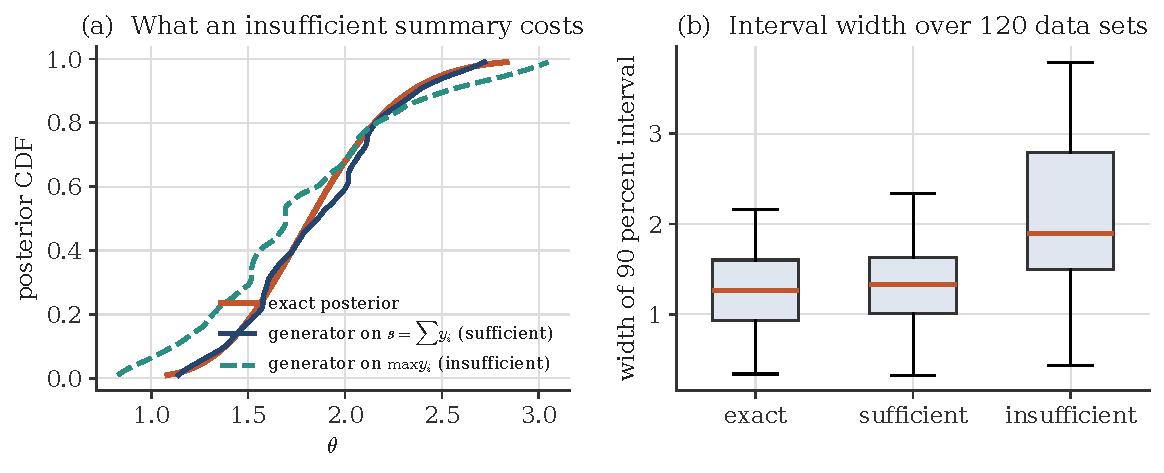
\includegraphics[width=0.9\textwidth]{app_sufficiency}
\caption{Sufficiency as dimension reduction. (a) Posterior distribution functions for one data set:
a generator trained on the sufficient total closely matches the exact posterior, while one trained on the
insufficient sample maximum does not. (b) Width of the ninety percent interval over one hundred and
twenty data sets; the insufficient summary inflates the interval by about half.}
\label{fig:app_sufficiency}
\end{figure}

Figure~\ref{fig:app_gbcpipeline} collects the whole construction. Training happens once: simulate
parameter and data pairs from the joint law, reduce each data set to its summary, and fit the map by
the check loss. Use is then immediate for any data set the model can produce: summarize, draw base
randomness, evaluate the map.

\begin{figure}[H]
\centering
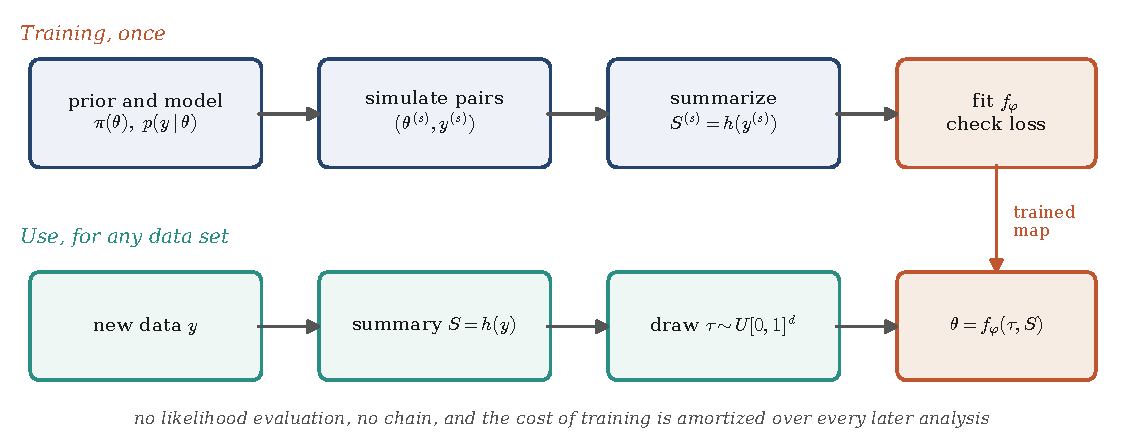
\includegraphics[width=0.95\textwidth]{app_gbcpipeline}
\caption{The generative Bayesian computation pipeline. The upper row is paid once; the lower row is
what an analysis costs thereafter. Sufficiency is what keeps the map's input small, and the check
loss is what makes the fitted map a posterior quantile map.}
\label{fig:app_gbcpipeline}
\end{figure}

\subsection{Quantile maps and multivariate transport}\label{gbp:sec:quantile}\index{Brenier map}\index{optimal transport}
In one dimension the map is the posterior quantile function and is monotone, which pins it down
uniquely. In several dimensions monotonicity must be replaced by something stronger, and the
natural choice is the Brenier map, the gradient of a convex potential, which is the unique
transport from the reference cube to the posterior that is optimal for squared cost. For a scalar parameter this is the
object the causal machinery of Section~\ref{ch:gbc} estimates (for a vector parameter its network, fitted by the pinball loss, estimates a triangular map with the same pushforward), and it is why the posterior map and
the optimal transport literature are the same subject seen from two sides.

For estimation, a practical architecture takes the base variable and the summary statistic as
inputs and returns the quantile. The base variable is not fed in raw but through an embedding, a
vector of cosine features of $\tau$, which lets a single network represent the whole family of
quantile levels at once rather than one level at a time. The summary enters through its own branch,
and the two are combined multiplicatively before a final stack of layers, a coupling that lets the
data reshape the entire quantile curve rather than merely shift it.

\subsection{Training by the check loss}\label{gbp:sec:training}
The map is fitted by quantile regression. Simulate $M$ pairs $(\theta^{(s)}, y^{(s)})$ from the joint
law, which requires only the ability to sample the prior and the model, compute summaries
$S^{(s)}=h(y^{(s)})$, draw levels $\tau_s$, and minimize the check loss
\[
 \mathcal{L}(\varphi) \;=\; \frac1M\sum_{s=1}^{M}
 \rho_{\tau_s}\!\bigl(\theta^{(s)} - f_\varphi(\tau_s, S^{(s)})\bigr),
 \qquad \rho_\tau(u) = u\bigl(\tau - \mathbf{1}\{u<0\}\bigr).
\]
Because the check loss is minimized at the conditional quantile, the fitted $f_\varphi$ converges to
the posterior quantile map, and no likelihood is ever evaluated. Two practical points deserve
emphasis. The estimated curve should be monotone in $\tau$, and fitted networks can violate this
slightly, a defect known as quantile crossing; projecting onto the monotone cone repairs it and
costs nothing. And the quality of the summary statistic governs everything, since a lossy summary
yields the posterior given that summary rather than the posterior given the data.

\subsection{Generative methods as transport estimation}\label{gbp:sec:transport}
Read this way, the modern generative toolkit is a single subject. Normalizing flows compose simple
invertible maps and track the Jacobian. Variational autoencoders learn a stochastic encoder and
decoder between a latent reference and the observation space. Diffusion models build the map as the
time reversal of a noising process. Generative adversarial networks fit the map by matching
distributions through a discriminator rather than by a likelihood. Each estimates a transport from
reference randomness to a target law, and they differ in the family of maps allowed and the
criterion used to fit it. The linear Gaussian case is instructive: there the optimal map is affine,
and the Kalman filter of Section~\ref{ch:filter} is exactly the generative update, which is why the
filter is the natural sanity check for any proposed generative scheme.

\subsection{Predictive resampling and the weighted bootstrap}\label{gbp:sec:bootstrap}
Generators are older than neural networks. The Bayesian bootstrap draws Dirichlet weights on the
observed points and reports the resulting functional, the weighted likelihood bootstrap attaches
random weights to the likelihood and optimizes, and both deliver posterior like draws by repeated
simulation with no chain. The Bayesian bootstrap is also predictive resampling: completing the population by draws from a P\'olya urn seeded with the observed points, each drawn point returned with a copy of itself, leaves $\mathrm{Dir}(1,\dots,1)$ weights on those points, so its draws are those of the martingale posterior of Fong, Holmes and Walker (2023) for that urn (Section~\ref{sec:mp-critique}). In the present language each is a generator with a fixed rather than a
learned map, and the accuracy question is how closely the induced law matches the posterior. These
schemes remain the most reliable generators when the model is low dimensional, and they supply the
benchmark against which a trained map should be judged.

\subsection{Decision, design, and risk sensitivity}\label{gbp:sec:decision}
The payoff is largest where a posterior is wanted not for display but for a decision. Since the
generator returns draws of the parameter, it returns draws of any utility built on it, so expected
utility is a sample average and the optimal action is an argmax over actions of a simulated
quantity. Risk sensitivity comes free: distorting the base measure, in the manner of the dual
theory of choice, converts the same draws into a conservative certainty equivalent, and reading the
lower tail gives a conditional value at risk criterion without a separate calculation. Sequential
problems fit the same mould, since a design or a policy is a Bellman backup over simulated futures,
and the generator is the simulator that backup requires. This is the route by which the
apparatus reaches experimental design, accelerated life testing, causal decisions in
Section~\ref{ch:gbc}, and reinforcement learning with verifiable rewards.

\subsection{A worked example: one network, every data set}\label{gbp:sec:worked}
Take $\theta\sim\mathrm{Gamma}(2,1)$ with $n=12$ conditionally Poisson observations, so the sufficient
statistic is the total count $s$ and the posterior is $\mathrm{Gamma}(2+s,\,1+12)$, known in closed form and
therefore available as ground truth. Nothing about that closed form is used in fitting. Sixty
thousand pairs are simulated from the joint law, a small network is trained by the check loss, and
the fitted map is then asked for posteriors at total counts it must interpolate between.
Figure~\ref{fig:app_gbc}(a) plots the learned map against the base uniform for three data sets,
with the exact quantile functions dashed: one network produces all three curves, and the data enter
only as an input. Panel (b) plots generator quantiles against exact quantiles across the
posterior, where the agreement is close over the central range and the visible departures
are confined to the extreme tails, which are the hardest levels for the check loss to resolve and
the region where simulated training data are thinnest.

\begin{figure}[H]
\centering
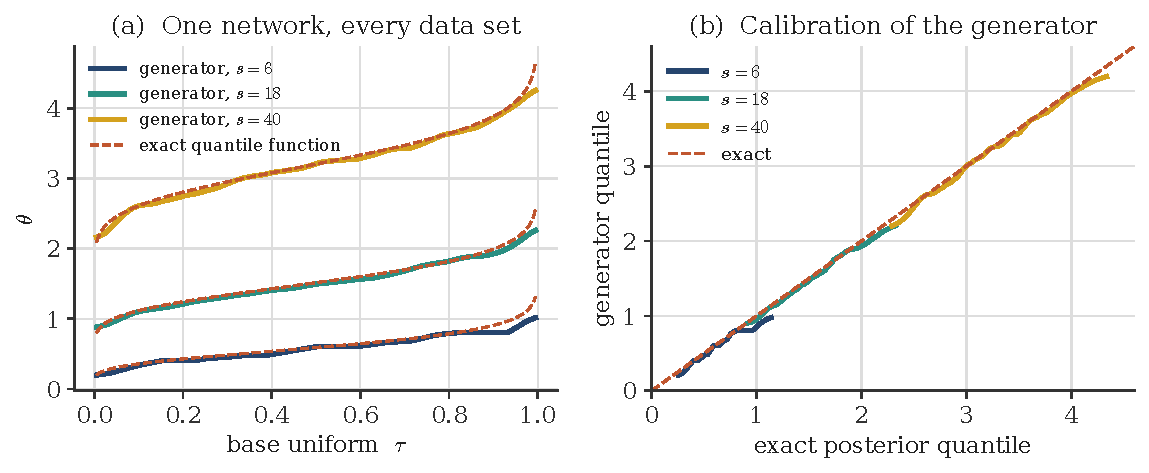
\includegraphics[width=0.9\textwidth]{app_gbc}
\caption{Generative Bayesian prediction on a conjugate model used only as ground truth. (a) The
learned map from the base uniform to the parameter, for three different data sets, against the
exact quantile functions (dashed). A single trained network produces all three. (b) Generator
quantiles against exact quantiles; the map is accurate across the central range and degrades only
in the extreme tails.}
\label{fig:app_gbc}
\end{figure}

\paragraph{Summary.} A posterior can be delivered as a sampler rather than as a density. Noise
outsourcing guarantees that a map from independent base randomness to the posterior exists and may
be taken to read the data only through a sufficient summary; quantile regression estimates it
without evaluating a likelihood; optimal transport identifies the multivariate version; and the
resulting generator amortizes across data sets and feeds decisions directly. The cost is moved from
the moment of analysis to a single training run, which is the right trade whenever the same model
will be applied many times.

\subsection*{Problems}
\begin{enumerate}[leftmargin=1.8em,itemsep=2pt]
\item Show that for a scalar parameter the noise outsourcing map $f(\tau,y)$ can be taken to be the posterior quantile function, and that it is then nondecreasing in $\tau$ for every $y$.
\item For the Gamma Poisson model of Section~\ref{gbp:sec:worked}, write the posterior quantile map explicitly and verify that it depends on the data only through the total count.
\item Prove that the check loss $\rho_\tau(u)=u(\tau-\mathbf{1}\{u<0\})$ is minimized in expectation by the conditional $\tau$ quantile, and explain why this makes the fitted network a posterior quantile map without any likelihood evaluation.
\item A fitted quantile network is observed to cross, giving a smaller value at $\tau=0.6$ than at $\tau=0.5$ for some data set. Describe the monotone projection that repairs it and argue that the projection cannot increase the check loss.
\item Train a generator on a summary that is not sufficient. Show that the law it produces is the posterior given the summary and that its variance is at least that of the exact posterior, in the sense of the law of total variance.
\item In the linear Gaussian model, show that the optimal transport from the prior to the posterior is affine, and identify the posterior it reaches with the Kalman update.
\end{enumerate}

\src{The generative Bayesian computation program of Polson and Sokolov: quantile maps and
transport for Bayesian computation; generative Bayesian computation for the risk sensitive design
of accelerated life tests (Polson, Sokolov and Soyer, 2026); generative maps for amortized inference
(Mira and Polson); generative Bayesian computation for dynamic spatial models (Gamerman and
Polson); the generative learner for distributional causal effects (Nareklishvili, Polson and
Sokolov, 2025); quantile generative computation for reinforcement learning with verifiable rewards
(Polson, Sokolov and Zantedeschi, 2026h); and uncertainty quantification from the weighted bootstrap to generators
(Lopes, Polson and Sokolov, 2025). The noise outsourcing representation follows Kallenberg (2002); the
multivariate transport reading follows Brenier; the implicit quantile architecture follows the
distributional reinforcement learning literature.}

\section[Double Descent and Ordered Empirical Bayes]{Double Descent, Ordered Empirical Bayes, and the Selection of Complexity}\label{ch:dd}\index{double descent}\index{interpolation threshold}\index{ordered empirical Bayes}\index{isotonic regression}\index{effective degrees of freedom}

\noindent\textbf{Thesis.} Model choice is a coding problem, and once complexity is measured in nats
rather than in parameters the modern puzzles dissolve. Adding parameters past the point where a
model interpolates its data improves prediction rather than destroying it, because what saturates
is not the parameter count but the effective complexity the evidence actually pays for. The
regularizer that makes this work is not a single global penalty but an ordered family of them,
estimated from the data, which is the empirical Bayes counterpart of the same accounting.

\subsection{The interpolation threshold}\label{dd:sec:threshold}
Classical model selection teaches a tradeoff: risk falls as a model grows, reaches a minimum, and
rises again as variance takes over. That curve is real, but it describes only the region where
parameters are scarcer than observations. Write $\psi=p/n$ for the ratio of parameters to sample
size. Figure~\ref{fig:app_doubledescent}(a) plots test risk in a random feature regression as $\psi$
grows through and beyond one. The classical arc appears on the left, the risk then explodes as
$\psi$ approaches one, and beyond the interpolation threshold it falls again toward
the noise floor, ending well below the best risk achieved in the classical region. The peak is not a
paradox but a conditioning failure: at $\psi=1$ the feature matrix is square and nearly singular, so
the minimum norm solution is forced through the data by enormous coefficients. Past that point there
are many interpolating solutions, the minimum norm criterion selects a smooth one, and the fit
improves. The second curve in the panel makes the diagnosis: a small ridge penalty removes the spike
almost entirely and leaves only a modest bump in its place. The peak is a symptom of
unregularized interpolation, not a property of large models.

\subsection{Complexity is what the evidence pays for}\label{dd:sec:complexity}
Panel (b) supplies the Bayesian reading. Plotting the effective degrees of freedom, the trace of the
smoother matrix, against $\psi$ shows it rising steeply while parameters are scarce and then
flattening at a ceiling set by the sample size. Doubling the parameter count past the threshold buys
almost no additional effective complexity. This is the quantity the marginal likelihood is sensitive
to, and it is the quantity the description length of Section~\ref{ch:mdl} charges for. A wide
network that settles in a flat basin admits a short code, as argued in Section~\ref{dl:sec:double},
and the evidence recovers once the model is wide enough for such a basin to
exist. Read this way, double descent is the evidence curve seen through a badly chosen horizontal
axis. Parameter count is a proxy that fails where it is being used, and codelength is the
measurement that does not. It also explains why the phenomenon is a threshold effect rather than a
gradual one, and why the position of the peak is governed by $\psi$ and not by the architecture.

\subsection{Ordered empirical Bayes as the default regularizer}\label{dd:sec:orderedeb}
If regularization is what tames the threshold, the question becomes which penalty to use, and the
honest answer is that a single global scale is rarely right. The global local priors of
Section~\ref{da:sec:bridge} already say so: coefficients differ, and a rule that shrinks all of them
by one common factor either flattens the real signals or leaves the noise standing. The empirical
Bayes version estimates the shrinkage weight from the data, but estimating a separate weight for
every coordinate simply transfers the noise from the estimate to the regularizer.

Ordering resolves the tension. The weight $1-\kappa_j$ that multiplies the observation should increase with the evidence for a signal,
so estimating it in bins of the ordering statistic $|z|$, which pools coordinates that carry similar evidence, and constraining the binned weights to be nondecreasing by
isotonic regression, gives a rule with the flexibility of a local method and the stability of a
global one. Figure~\ref{fig:app_orderedeb}(a) shows the mechanism: the unconstrained local estimates
scatter badly, the isotonic fit passes through them as a monotone staircase, and the single global
weight is the flat line that cannot adapt. Panel (b) gives the consequence in risk. Against a mean
squared error of $1.01$ for no shrinkage, the global rule reaches $0.47$ and the ordered rule
$0.30$, a further reduction of a third. Nearly all of it comes from letting the weight vary across the bins: the bin estimates without the monotone constraint already reach $0.309$ against $0.304$ for the isotonic fit, so in this simulation monotonicity lowers the risk by under two percent, and what it adds is a profile that never shrinks a larger $|z|$ harder than a smaller one. Nothing here was
tuned by hand, which is the sense in which the ordered rule is a default rather than a choice.

\subsection{Why this is an information theoretic story}\label{dd:sec:info}
The two halves of the section are one argument. A description length has two parts, the cost of
stating the model and the cost of stating the data given it, and every result above is an instance
of that split. Effective complexity is the first part measured properly, which is why it saturates
while parameter count does not. Shrinkage is the first part made adaptive, and an ordered profile is
the cheapest description of a family of scales that respects the obvious constraint that stronger
evidence deserves less shrinkage. The evidence, the description length, and the risk curves are
three views of one accounting, and the moderate deviation scale that runs through this book is where
the accounting is settled: a coordinate is retained when its evidence crosses the threshold that
balances the two costs, and the ordered profile is the estimated form of that threshold.

Two practical consequences follow. First, a large model should not be rejected on parameter count,
and selection criteria that charge per parameter will mislead in the interpolating regime; the
evidence, or a codelength surrogate for it, is the criterion that survives. Second, the regularizer
should be estimated rather than fixed, and estimated along the ordering of the evidence rather than freely.
These are the recommendations the score matching and generative literature arrives at from a
different direction, where the same ordered empirical Bayes profile serves as the default penalty
for score based models and for reinforcement learning with verifiable rewards.

\begin{figure}[H]
\centering
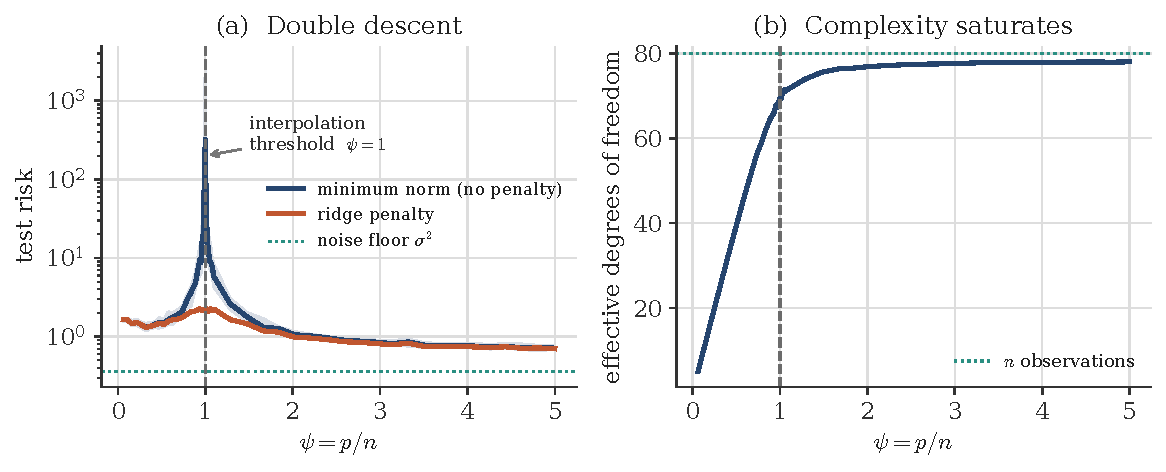
\includegraphics[width=0.9\textwidth]{app_doubledescent}
\caption{Double descent in a random feature regression. (a) Test risk against $\psi=p/n$ on a
logarithmic scale, with the interquartile band over replications. The risk spikes at the
interpolation threshold and then falls below its classical minimum; a small ridge penalty removes
the spike. (b) Effective degrees of freedom against $\psi$, which saturate near the sample size:
past the threshold, extra parameters buy almost no extra complexity.}
\label{fig:app_doubledescent}
\end{figure}

\begin{figure}[H]
\centering
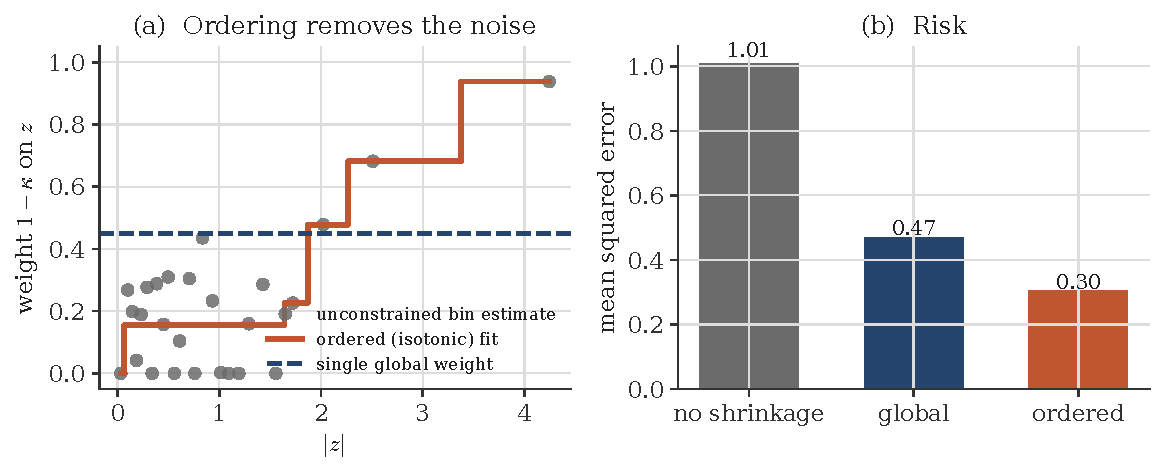
\includegraphics[width=0.9\textwidth]{app_orderedeb}
\caption{Ordered empirical Bayes. (a) Bin estimates of the weight $1-\kappa$ on the observation, made from an independent
measurement, scatter badly; the isotonic fit recovers a monotone profile, and a single global weight
cannot adapt. (b) Mean squared error for no shrinkage, a global weight, and the ordered rule.}
\label{fig:app_orderedeb}
\end{figure}

\paragraph{Summary.} Past the interpolation threshold, risk falls again because effective
complexity, not parameter count, is what the evidence charges for, and effective complexity
saturates. The regularizer that exploits this is an estimated shrinkage profile constrained to be
monotone in the evidence, which beats both no shrinkage and a single global scale without tuning.
Model selection, on this reading, is description length accounting carried out on the right axis.

\subsection*{Problems}
\begin{enumerate}[leftmargin=1.8em,itemsep=2pt]
\item For least squares with $p$ features and $n$ observations, show that the minimum norm solution interpolates the data when $p>n$ and compute the expected test risk when the features are isotropic Gaussian, exhibiting the divergence at $p=n$.
\item Show that the trace of the ridge smoother matrix is bounded by $n$ for every $p$, and interpret the bound as a statement about effective complexity.
\item Explain why a small ridge penalty removes the spike at the interpolation threshold, and relate the penalty to a Gaussian prior on the coefficients.
\item Let $z_i=\mu_i+\varepsilon_i$ with independent standard normal errors and $\mu_i$ a scale mixture of normals. Derive the oracle weight $\E[\mu_i\mid z_i]/z_i$ for a coordinate as a function of $|z_i|$ and show that it is nondecreasing, which is the constraint ordered empirical Bayes imposes.
\item Implement the pool adjacent violators algorithm and verify that it returns the isotonic least squares fit. Apply it to noisy bin estimates of shrinkage weights and compare the risk to a single global weight.
\item Write the two part codelength for a sparse regression and show that the ordered shrinkage profile corresponds to a monotone cost of describing the coefficients.
\end{enumerate}

\src{Bayesian Double Descent (Polson and Sokolov, 2025); Ordered Empirical Bayes: A Default Regularizer
for Score-Based Generative Models (Polson, Sokolov and Zantedeschi, 2026g); the global local regularization program of
Datta, Polson and Sokolov (2025); Carvalho, Polson and Scott (2010) on the horseshoe; Rissanen (1978) and
Watanabe (2009) for the description length and singular evidence accounting of
Section~\ref{ch:mdl}.}


\section{Proximal Algorithms and Optimization as Inference}\label{ch:proximal}

\noindent\textbf{Thesis.} The optimization that produces a penalized point estimate
and the Monte Carlo that produces a posterior are the two faces of one object, the
proximal operator. Regularized estimators, the lasso, total-variation
denoising, are fixed points of proximal maps; the proximal map is itself
the mode of a Gaussian-plus-penalty posterior; and the same envelope that makes a
nonsmooth penalty differentiable makes it a location mixture that can be sampled. This
short section reads the modern optimization toolkit, proximal gradient, ADMM,
Douglas--Rachford, as inference, the optimization counterpart of the data
augmentation of Section~\ref{ch:augment}.

\subsection{The proximal operator}\label{px:sec:prox}

For a closed convex penalty $\phi$ and step $t>0$, the \emph{proximal operator} is
\[
\mathrm{prox}_{t\phi}(v)=\argmin_{\theta}\Big\{\phi(\theta)+\tfrac{1}{2t}\|\theta-v\|^2\Big\}.
\]
It is the resolvent of the subdifferential, $(\,I+t\partial\phi)^{-1}$, and it is
firmly nonexpansive, so iterating it converges to a minimizer of $\phi$ when one exists. Two readings sit on top of this one
definition. Analytically, $\mathrm{prox}_{t\phi}(v)$ is the value that trades a
decrease in $\phi$ against staying near $v$, and for the $\ell_1$ penalty it is exactly
soft-thresholding, $\mathrm{prox}_{t|\cdot|}(v)=\mathrm{sgn}(v)\max(|v|-t,0)$, the
operation at the heart of the lasso. Statistically, $\mathrm{prox}_{t\phi}(v)$ is the
posterior mode of $\theta\mid v$ under the model $v\mid\theta\sim\N(\theta,t)$ and
prior $\pi(\theta)\propto e^{-\phi(\theta)}$: the proximal step is a MAP estimate of a
Gaussian observation with a log-prior penalty. The two readings are the same
computation, and this is why every penalized estimator in the book has both an
optimization algorithm and a sampler.

\subsection{Proximal gradient and its Bayesian reading}\label{px:sec:pg}

To minimize $\ell(\theta)+\phi(\theta)$ with $\ell$ smooth and $\phi$ nonsmooth, the
proximal-gradient iteration takes a gradient step on $\ell$ and a proximal step on
$\phi$,
\[
\theta^{k+1}=\mathrm{prox}_{t\phi}\!\big(\theta^k-t\nabla\ell(\theta^k)\big).
\]
For $\ell$ a Gaussian negative log-likelihood and $\phi$ the $\ell_1$ penalty this is
iterative soft-thresholding, the workhorse of sparse regression. Its inferential
counterpart replaces the deterministic proximal step by a draw from the corresponding
Gaussian-plus-penalty conditional: the Moreau--Yosida envelope of $\phi$,
$\phi_t(v)=\min_\theta\{\phi(\theta)+\tfrac1{2t}\|\theta-v\|^2\}$, is a smooth
approximation whose gradient is $(v-\mathrm{prox}_{t\phi}(v))/t$, and the envelope is
the low-temperature limit of the negative log of a location-mixture density, a Gaussian convolved with $e^{-\phi}$. Sampling
under the envelope is therefore the data augmentation of Section~\ref{ch:augment}
with the center $\theta$ of the mixture as the latent. Given $v$, the latent has the Gaussian-plus-penalty law $\propto e^{-\phi(\theta)-\|\theta-v\|^2/(2t)}$, whose mode is $\mathrm{prox}_{t\phi}(v)$, and by Tweedie's formula (Section~\ref{rg:sec:tweedie}) the negative log of the mixture has gradient $(v-\E[\theta\mid v])/t$, the envelope gradient with the conditional mean of the latent in place of its mode. A two-block sampler alternates a draw of $v$ from $e^{-\ell(v)}\N(v\mid\theta,t)$ with this draw of $\theta$; replacing both draws by their modes, with $\ell$ linearized at the current point so that the first mode is the gradient step $\theta-t\nabla\ell(\theta)$, gives back proximal-gradient descent, which is in this sense the
mode path of that sampler. Optimization returns the mode; the augmented chain returns
the spread around it.

\subsection{ADMM and Douglas--Rachford as splitting}\label{px:sec:admm}

When the objective splits as $f(\theta)+g(z)$ subject to a linear constraint, the
alternating direction method of multipliers alternates a proximal step in $\theta$, a
proximal step in $z$, and a dual update. The two proximal steps are two conditional
MAP problems, and the dual variable is the Lagrange multiplier that couples them; the
iteration is Douglas--Rachford splitting on the dual. Read as inference this is a
block Gibbs sampler in which each proximal step becomes a draw from a conditional
posterior and the multiplier tracks the constraint, so ADMM is the optimization
shadow of a two-block augmentation like the P\'olya--Gamma scheme of
Section~\ref{ch:augment}. The practical payoff is modularity: a complicated composite
penalty is handled by splitting it into pieces each of which has a closed-form
proximal map or a conjugate complete conditional, and the same split serves both the
optimizer and the sampler. Estimation and uncertainty quantification run on one
architecture, which is the recurring lesson of this chapter: the algorithm
that finds the mode and the algorithm that explores the posterior differ only in
whether the proximal step is taken or sampled.


\subsection*{Worked example: soft-thresholding and the Huber envelope}
This example computes the proximal map, the Gaussian-plus-penalty posterior mode and the Moreau--Yosida envelope of the $\ell_1$ penalty in closed form.

Take $\phi(\theta)=|\theta|$ and the step $t=\tfrac12$, so that $\mathrm{prox}_{t\phi}$ is soft-thresholding at $\tfrac12$. Then $\mathrm{prox}_{t\phi}(0.3)=0$, because the observation lies inside the threshold, and $\mathrm{prox}_{t\phi}(2)=1.5$. These are the posterior modes of $\theta\mid v$ under $v\mid\theta\sim\N(\theta,\tfrac12)$ and the Laplace prior $\pi(\theta)\propto e^{-|\theta|}$: the mode minimizes $|\theta|+(\theta-v)^2$, which gives the corner $\theta=0$ with value $0.09$ at $v=0.3$ and $\theta=1.5$ with value $1.75$ at $v=2$. Those two values are the Moreau--Yosida envelope $\phi_t(v)$, which here is the Huber function $\phi_t(v)=v^2/(2t)$ for $|v|\le t$ and $|v|-t/2$ for $|v|>t$. Its gradient $(v-\mathrm{prox}_{t\phi}(v))/t$ equals $0.6$ at $v=0.3$ and $1$ at $v=2$, the clipped value $\max\{-1,\min\{1,v/t\}\}$ of $v/t=0.6$ and $v/t=4$. The proximal step is thus the Laplace posterior mode, and the Huber function is the smooth envelope whose gradient is the scaled proximal residual.

\paragraph{Summary.}
The proximal operator is the resolvent of the subdifferential and, equivalently, the MAP estimate of a Gaussian observation under a log-prior penalty. Proximal-gradient, ADMM, and Douglas--Rachford splitting are optimization shadows of Gibbs samplers, so estimation and uncertainty run on one architecture.

\subsection*{Problems}
\begin{enumerate}[leftmargin=2.2em,itemsep=2pt]
\item Show $\mathrm{prox}_{t|\cdot|}(v)=\mathrm{sgn}(v)\max(|v|-t,0)$ (soft-thresholding).
\item Prove the proximal operator is firmly nonexpansive.
\item Identify $\mathrm{prox}_{t\phi}(v)$ as the posterior mode under $v\mid\theta\sim\N(\theta,t)$ and $\pi\propto e^{-\phi}$.
\item Derive the ADMM updates for the lasso and interpret the dual variable as a Lagrange multiplier.
\item Show that the Moreau envelope is, in the low-temperature limit, the negative log of a Gaussian-convolved prior and relate its gradient to the proximal residual.
\end{enumerate}

\src{Proximal Algorithms in Statistics and Machine Learning (Polson, Scott and
Willard, 2015); the data-augmentation view of Section~\ref{ch:augment}; global-local
shrinkage of Section~\ref{ch:hsmdp}.}

%====================================================================================================

\shorthead{Regularization and Nonparametric Models}
\chapter{Regularization, Nonparametric Models, and Averaging}\label{chap:regularization}

Every penalty is a prior, and every prior is a predictive commitment. This chapter develops the
shrinkage estimators, discrete-choice models, and averaging rules that put the synthesis to work.
Tweedie's formula gives the posterior mean as a score correction and makes the choice of prior a choice
of tail behavior; discrete choice reads utility maximization as latent-variable prediction; and model
averaging, rather than model selection, is the log-loss-optimal way to carry model uncertainty into the
predictive.
Split sampling, slice sampling, and variational inference supply the computation; Gaussian processes, trees, Dirichlet-process mixtures, and hierarchical models extend the same predictive rule to functions, distributions, and groups, with the kernel or the depth prior in the role of the scale and the marginal likelihood in the role of Occam's razor; and model criticism closes the chapter by asking whether the observed data look like a plausible draw from the fitted model.

The theme throughout is that regularization is not an add-on to inference but the predictive content of
a prior, and that the same shrinkage geometry, a spike for the null coordinates and a tail for the
signal, governs estimation, selection, and averaging alike.


\shorthead{Regularization, Sparse Recovery, and Empirical Bayes}
\section{Bayesian Regularization, Sparse Recovery, and Empirical Bayes}\label{ch:regular}

\noindent\textbf{Thesis.} Every penalty is a prior, every regularization path is a
posterior, and the right amount of shrinkage is not tuned but learned. This section
gathers the global-local view of sparse estimation into one statement: a shrinkage
estimator is a posterior mean under a scale-mixture prior, its risk is governed by
how the prior treats the origin and the tails, and the global scale that controls
overall sparsity is itself estimated from the data by an empirical-Bayes or
full-Bayes rule. It is the synthesis of the horseshoe, bridge, and lasso threads of
Sections~\ref{ch:hsmdp} and~\ref{ch:augment}, read as one decision problem.

\subsection{Penalties are priors}\label{rg:sec:penalty}

A penalized estimator $\hat\theta=\argmin_\theta\{\tfrac1{2}\|y-\theta\|^2+\mathrm{pen}(\theta)\}$
is the posterior mode under the prior $\pi(\theta)\propto e^{-\mathrm{pen}(\theta)}$ and
a unit-variance Gaussian likelihood. Ridge is a Gaussian prior, the lasso a Laplace
prior, the bridge a stable-mixture prior, and the horseshoe a half-Cauchy scale
mixture. The point estimate is only the mode; the posterior carries the rest, and
for prediction the posterior mean is what minimizes squared-error risk. The
global-local representation $\theta_j\mid\lambda_j,\tau\sim\N(0,\lambda_j^2\tau^2)$
with a prior on the local scales $\lambda_j$ and a global scale $\tau$ makes the
whole family a single hierarchical model: the local scales decide which coordinates
escape shrinkage, and the global scale sets the overall level. The tail of the local
prior is the estimator's identity, exponential tails shrink everything a little,
polynomial tails leave large signals essentially untouched, and the behavior at the
origin decides how aggressively noise is killed.

\subsection{Tweedie's formula and empirical Bayes}\label{rg:sec:tweedie}

The posterior mean under any prior has a closed form in terms of the marginal
density. For $y\mid\theta\sim\N(\theta,1)$ with marginal $m(y)=\int\N(y\mid\theta,1)\pi(\theta)\,d\theta$,
Tweedie's formula gives
\[
\E[\theta\mid y]=y+\frac{d}{dy}\log m(y),
\]
so the Bayes estimator is the observation plus the score of its own marginal. This is
the empirical-Bayes engine: estimate the marginal $m$ from the pooled data, take its
log-derivative, and the shrinkage rule follows without ever naming the prior. It
explains why global-local priors adapt (the score of a heavy-tailed marginal is
near zero in the tails, so large observations are barely moved), and it connects
shrinkage to the coding view, since $-\log m(y)$ is the codelength the marginal
assigns and its negative derivative is the local shrinkage force. The global scale $\tau$ is
chosen by maximizing the same marginal likelihood, the empirical-Bayes estimate, or
by placing a half-Cauchy hyperprior on it and integrating, the full-Bayes rule; the
empirical-Bayes estimate can collapse to $\hat\tau=0$ under sparsity unless it is bounded away from zero (Section~\ref{hs:sec:tau}), a degeneracy the full-Bayes rule avoids.

\subsection{Risk and the oracle}\label{rg:sec:risk}

Under sparsity, most coordinates zero, a few large, the target is the risk of the
oracle that knows which coordinates are nonzero. The horseshoe and its relatives
attain that oracle risk up to a logarithmic factor, because their marginal prior has the two
properties Tweedie's formula rewards: an infinite spike at the origin, which drives
the score to shrink noise coordinates essentially to zero, and Cauchy-heavy tails,
which flatten the score so signal coordinates are returned near their observed
values. With $p_0$ nonzero coordinates among $n$ and unit noise, the oracle's total squared-error risk is $p_0$, while no estimator that must find the support itself can beat the minimax rate $p_0\log(n/p_0)$, which the horseshoe attains with a suitably small global scale (van der Pas, Kleijn and van der Vaart, 2014). Datta and Ghosh (2013) show that the horseshoe attains the zero-one oracle risk of Theorem~\ref{hs:thm:oracle} up to a constant, but that is a testing risk, not this estimation risk. The bridge and lasso trade some of this adaptivity for a global
tuning parameter, the lasso also for convexity, which the bridge penalty $\sum_j|\theta_j|^{\alpha}$ has only for $\alpha\ge1$. The moderate-deviation analysis of Section~\ref{ch:hsmdp} makes the
comparison sharp: the effective shrinkage threshold grows like the square root of the
log of the inverse sparsity proportion $n/p_0$, the sparse analogue of the testing threshold of
Section~\ref{ch:deviations}, so sparse recovery and Bayesian testing are the same
moderate-deviation calculation with $n/p_0$ playing the role of the sample
size.


\subsection{A field guide to shrinkage priors}\label{rg:sec:guide}

The global-local family is easiest to read as one table. Each row is a prior on the
local scale $\lambda_j$ (the half-Cauchy row), on the local variance $\lambda_j^2$ (the exponential and inverse-gamma rows) or on the local precision $\lambda_j^{-2}$ (the stable row); the induced marginal on $\theta_j$, its behavior at the
origin and in the tails, and the estimator it reproduces follow from it.

\begin{table}[h]\centering
\begin{tabular}{@{}lllll@{}}
\toprule
Local prior & Marginal on $\theta_j$ & Origin & Tail & Estimator \\
\midrule
Point mass & Gaussian & finite & Gaussian & ridge \\
Exponential & Laplace & finite & exponential & lasso \\
Stable & bridge & finite & stretched exp. & bridge \\
Half-Cauchy & horseshoe & $+\infty$ & polynomial & horseshoe \\
Inverse-gamma & Student-$t$ & finite & polynomial & relevance vector \\
\bottomrule
\end{tabular}
\caption{Global-local shrinkage priors. An infinite spike at the origin drives noise
coordinates to zero; a polynomial tail leaves large signals unshrunk. The horseshoe is
the boundary case with both. The bridge row takes the marginal $e^{-|\theta_j|^{\alpha}}$ with $0<\alpha<1$ (Section~\ref{da:sec:bridge}), the range in which its tail is stretched exponential.}\label{rg:tab:priors}
\end{table}

\noindent The two columns that matter for risk are the origin and the tail. A prior
with an infinite spike at the origin, like the horseshoe, produces a Tweedie score that
shrinks small observations essentially to zero; a polynomial tail flattens the score
for large observations, so signals are returned near their data values. The lasso's
finite spike and exponential tail explain both its bias on large signals and its
failure to shrink noise as aggressively as the horseshoe, the gap the
moderate-deviation analysis of Section~\ref{ch:hsmdp} makes precise.





\subsection*{Worked example: spike-and-slab shrinkage via Tweedie}
This example shows a two-group prior producing the selective shrinkage that sparse problems need.

Take the Gaussian sequence $y_j\sim\N(\theta_j,1)$ with a spike-and-slab marginal $m(y)=(1-w)\phi(y)+w\,\phi_\tau(y)$, $\phi$ and $\phi_\tau$ the $\N(0,1)$ and $\N(0,1+\tau^2)$ densities. Tweedie gives $\E[\theta_j\mid y]=y+m'(y)/m(y)$; for large $|y|$ the slab dominates and $\E[\theta\mid y]\approx y\,\tau^2/(1+\tau^2)$ (little shrinkage for a diffuse slab, $\tau$ large), while for small $|y|$ the spike dominates and the estimate is pulled sharply to $0$. This is the two-groups model whose continuous relaxation is the horseshoe of Section~\ref{ch:hsmdp}.

The behavior is the discrete cousin of the horseshoe: small observations are pulled toward zero by the spike, while large ones are shrunk only by the slab factor $\tau^2/(1+\tau^2)$ and so survive nearly intact. Tweedie turns the choice of prior into the shape of the marginal, and the marginal's score is the shrinkage.

\paragraph{Summary.}
Every penalty is a prior; the posterior mean under a scale-mixture prior is the shrinkage estimator, given in closed form by Tweedie's formula $\E[\theta\mid y]=y+\tfrac{d}{dy}\log m(y)$. The global scale is learned by empirical or full Bayes, and heavy-tailed local priors with enough mass near zero attain the sparse oracle risk up to a logarithmic factor.

\subsection*{Problems}
\begin{enumerate}[leftmargin=2.2em,itemsep=2pt]
\item Prove Tweedie's formula for the Gaussian sequence model.
\item Show that ridge, lasso, and horseshoe correspond to a point mass, an exponential prior on the local variance $\lambda_j^2$, and a half-Cauchy prior on the local scale $\lambda_j$.
\item Explain why an infinite spike at the origin and a polynomial tail are the two properties Tweedie's score rewards.
\item Derive the empirical-Bayes estimate of the global scale by marginal-likelihood maximization.
\item Show the sparse threshold grows like $\sqrt{\log(1/p)}$ as the sparsity proportion $p\to0$ and connect to Section~\ref{ch:hsmdp}.
\end{enumerate}

\src{The Horseshoe Estimator for Sparse Signals (Carvalho, Polson and Scott, 2010);
Shrink Globally, Act Locally (Polson and Scott, 2010); On the Half-Cauchy Prior
(Polson and Scott, 2012b); Local Shrinkage Rules, L\'evy Processes and Regularized
Regression (Polson and Scott, 2012a); the empirical-Bayes/Tweedie tradition; and the
MDP analysis of Section~\ref{ch:hsmdp}.}

%====================================================================================================

\shorthead{Discrete Choice and Multinomial Probit}
\section{Discrete Choice, Multinomial Probit, and Latent Utility}\label{ch:choice}

\noindent\textbf{Thesis.} A discrete choice is the argmax of a latent utility, and
Bayesian inference for choice models is inference for the Gaussian or P\'olya--Gamma
latent that sits underneath the observed decision. This section treats the two
canonical constructions, the multinomial probit through a Gaussian latent utility
and the multinomial logit through P\'olya--Gamma augmentation, as instances of the
data-augmentation principle of Section~\ref{ch:augment}, and connects them to the
economics of the decision sections.

\subsection{Latent utility and the choice probability}\label{ch:sec:util}

A decision maker facing $J$ alternatives assigns each a latent utility
$U_j=x_j^\top\beta+\varepsilon_j$ and chooses the argmax. The distribution of the
error vector $\varepsilon$ fixes the model: i.i.d.\ extreme-value errors give the
multinomial logit with its closed-form softmax choice probabilities, while a Gaussian
error vector with covariance $\Sigma$ gives the multinomial probit, whose choice
probabilities are orthant integrals with no closed form. The logit's convenience
comes at the price of the independence-of-irrelevant-alternatives property, which the
probit's correlated errors avoid; the cost is that the probit likelihood is an
intractable Gaussian integral. Data augmentation removes the cost. Treating the
latent utilities as missing data, their complete conditional given the choice is a
truncated multivariate Gaussian, truncated to the cone where the chosen
alternative's utility is largest, and the parameters $(\beta,\Sigma)$ have conjugate
complete conditionals given the utilities. The multinomial probit thus fits by a
Gibbs sampler over truncated-Gaussian utilities and Gaussian-inverse-Wishart
parameters, the data augmentation of Section~\ref{ch:augment} applied to choice.

\subsection{P\'olya--Gamma multinomial logit}\label{ch:sec:pg}

The logit admits its own augmentation. With covariates $x$ and category-specific coefficients $\beta_j$, write the multinomial through a
one-versus-rest sequence of binomial factors: given the coefficients of the other categories, the likelihood of $\beta_j$ is a
logistic likelihood in the linear predictor $x^\top\beta_j-\log\sum_{k\neq j}e^{x^\top\beta_k}$, and the P\'olya--Gamma scheme of
Section~\ref{ch:augment} makes each $\beta_j$ conditionally Gaussian. A stick-breaking sequence of logistic factors, each linear in its own predictor, defines a different multinomial model, whose category probabilities are not a softmax of linear predictors and depend on the order of the categories. The multinomial logit
then fits by the same tuning-free two-block sampler, P\'olya--Gamma latents and
Gaussian coefficients, with the categories handled in sequence. This is the route
that carries choice models into hierarchical and spatial settings, where random
coefficients vary across individuals or regions and the top of the hierarchy is
Gaussian, so the whole model stays conditionally conjugate.

\subsection{The economics of the latent}\label{ch:sec:econ}

The latent-utility representation is not only a computational device; it is the
economic content. Willingness to pay, substitution patterns, and welfare changes are
all functionals of the utility parameters $\beta$ and the error covariance $\Sigma$,
and because the sampler returns their full posterior, these quantities come with
honest uncertainty rather than plug-in point estimates. Elasticities and market
shares are posterior predictive functionals of the choice probabilities, computed by
averaging over the posterior draws, and parameter uncertainty appears here as wider intervals on predicted shares. Discrete
choice is thus the microeconometric face of the predictive, decision-theoretic
program: the model is specified through a latent, fit by augmentation, and used
through the predictive distribution of the decision.




\subsection*{Worked example: logit choice and irrelevant alternatives}
This example exhibits both the softmax choice rule and its most famous limitation in one calculation.

Three alternatives with utilities $x^\top\beta=(1,0.5,0)$ give logit choice probabilities $\propto(e^1,e^{0.5},e^0)=(2.72,1.65,1)$, i.e.\ $(0.51,0.31,0.19)$. Removing alternative~3 rescales the first two to $(0.62,0.38)$, preserving their ratio, the independence-of-irrelevant-alternatives property that a correlated-error probit would break.

The preserved ratio is the independence of irrelevant alternatives: the logit's odds between any two options do not depend on what else is offered, a convenience for estimation and a liability when options are close substitutes. Reading choice as latent-utility prediction shows both where the property comes from and how nested or mixed logits relax it.

\paragraph{Summary.}
A discrete choice is the argmax of a latent utility; probit uses Gaussian errors (orthant-integral choice probabilities) and logit uses Gumbel errors (softmax). Both fit by data augmentation, truncated-Gaussian utilities for probit, P\'olya--Gamma for logit.

\subsection*{Problems}
\begin{enumerate}[leftmargin=2.2em,itemsep=2pt]
\item Show that i.i.d.\ Gumbel utility errors give softmax choice probabilities.
\item Derive the truncated-multivariate-Gaussian complete conditional for the latent utilities in the probit model.
\item Explain the independence-of-irrelevant-alternatives property of logit and how correlated probit errors avoid it.
\item Set up the P\'olya--Gamma sampler for multinomial logit via the one-versus-rest factorization, and show that a stick-breaking factorization with a linear predictor in each factor defines a different model.
\item Compute a market share and its posterior uncertainty as a predictive functional.
\end{enumerate}

\src{A Bayesian Analysis of the Multinomial Probit Model with Fully Identified Parameters (McCulloch, Polson and Rossi, 2000);
Bayesian Inference for Logistic Models Using P\'olya--Gamma Latent Variables (Polson,
Scott and Windle, 2013); the data-augmentation view of Section~\ref{ch:augment}.}

%====================================================================================================

\shorthead{Rare-Event Simulation, Split and Slice Sampling}
\section{Rare-Event Simulation, Split Sampling, and Slice Sampling}\label{ch:sim}

\noindent\textbf{Thesis.} Two hard simulation problems recur throughout Bayesian
computation, estimating a normalizing constant and drawing from an awkward
conditional, and both are solved by introducing an auxiliary variable that turns the
hard problem into a sequence of easy ones. Split sampling estimates rare-event
probabilities and normalizing constants by tempering through a ladder of intermediate
distributions; slice sampling\index{slice sampling} draws from any density by sampling uniformly under its
graph. Both are auxiliary-variable methods in the spirit of Section~\ref{ch:augment},
and both underlie the samplers used elsewhere in the book.

\subsection{Normalizing constants and rare events}\label{sm:sec:norm}

The evidence of a model is a normalizing constant, and a rare-event probability is a
normalizing constant of a restricted distribution; estimating either by naive Monte
Carlo fails when the target region carries little mass. Split sampling bridges from an
easy reference distribution to the hard target through a ladder of intermediate
distributions, each close enough to the next that importance weights are stable, and
multiplies the successive ratios to recover the constant. The intermediate ladder is
the same tempering that thermodynamic integration and annealed importance sampling
use, organized so that the rare event is reached in a sequence of likely steps rather
than one unlikely leap. The estimator's variance is controlled by the overlap between
adjacent rungs, which is why the ladder is chosen adaptively to keep the effective
sample size roughly constant along the path.

\subsection{Slice sampling}\label{sm:sec:slice}

To draw from a density $f(\theta)\propto g(\theta)$, slice sampling augments with a
height variable $u$ and samples uniformly from the region under the graph,
$\{(\theta,u):0<u<g(\theta)\}$. The two complete conditionals are both uniform: given
$\theta$, draw $u$ uniformly on $(0,g(\theta))$; given $u$, draw $\theta$ uniformly on
the slice $\{\theta:g(\theta)>u\}$. The chain requires no tuning of a proposal scale,
adapts automatically to the local width of the target, and is the default when a
conditional in a larger Gibbs sampler is nonstandard but one-dimensional. It is the
auxiliary-variable principle in its purest form: the awkward one-dimensional draw
becomes two uniform draws once the height is made explicit. The optimization
counterpart replaces the uniform slice draw by a maximization over the slice, turning
the same construction into a global optimizer that escapes local modes by climbing
through the level sets.

\subsection{Auxiliary variables as a unifying device}\label{sm:sec:aux}

Split sampling, slice sampling, and the data augmentation of Section~\ref{ch:augment}
are one idea: enlarge the state space with a latent whose conditional draws are easy,
so that marginalizing the latent recovers the hard target. The P\'olya--Gamma scheme
makes a binomial likelihood Gaussian; the slice variable makes an arbitrary density
uniform; the split ladder makes a rare event likely. In each the payoff is the same
trade the whole book keeps making, accept a larger model in exchange for tractable
conditionals, and the auxiliary variable is the price and the mechanism at once.


\subsection*{Worked example: a tail probability by a ladder, and a slice draw}
This example runs both devices on densities with known answers, so that the arithmetic can be checked by hand.

To estimate $\Prob(Z>4)$ for $Z\sim\N(0,1)$, climb the thresholds $0,1,2,3,4$, multiplying the probability $0.5$ of clearing $0$ by the probability of clearing each next threshold given the one before: $0.5\times0.3173\times0.1434\times0.0593\times0.0235=3.17\times10^{-5}=\Prob(Z>4)$. A naive sample of $10^4$ draws from $\N(0,1)$ expects $0.32$ draws above $4$, whereas $10^4$ draws from $Z\mid Z>3$ expect about $235$, so every factor is estimated from many hits and the factors multiply to the constant.

For the slice sampler take $g(\theta)=e^{-\theta}$ on $\theta>0$, whose area $1$ is the normalizing constant. Given $u\in(0,1)$ the slice is $(0,-\log u)$, so $\theta\mid u$ is uniform on it. Under the uniform law on the region under the graph, $\theta$ has density $\int_0^{e^{-\theta}}du=e^{-\theta}$, the target, and $u$ has density $-\log u$, the length of its slice. As a check, $\E[\theta]=\E[-\log u]/2=\tfrac12\int_0^1(\log u)^2\,du=1$, the mean of the target.

\paragraph{Summary.}
Auxiliary-variable methods turn a hard simulation into easy conditionals: split sampling reaches a rare event through a tempering ladder, and slice sampling draws uniformly under the density's graph. Both are the augmentation principle applied to normalizing constants and awkward draws.

\subsection*{Problems}
\begin{enumerate}[leftmargin=2.2em,itemsep=2pt]
\item Show that split sampling estimates a normalizing constant as a product of tractable ratios along a ladder.
\item Derive the two uniform complete conditionals of the slice sampler and prove it targets the density.
\item Explain how the tempering ladder is chosen to keep the effective sample size roughly constant.
\item Relate split sampling to thermodynamic integration and annealed importance sampling.
\item Show that the slice sampler needs no proposal-scale tuning and adapts to the local target width.
\end{enumerate}

\src{Split Sampling: Expectations, Normalisation and Rare Events (Birge, Chang and
Polson, 2012); Optimisation via Slice Sampling (Birge and Polson, 2012); the
auxiliary-variable view of Section~\ref{ch:augment}; Neal's slice sampler (2003).}

%====================================================================================================

\section{Bayesian Model Averaging and Predictive Distributions}\label{ch:bma}

\noindent\textbf{Thesis.} The right response to model uncertainty is not to choose a
model but to average over models, weighting each by its posterior probability, and
the object that results is a predictive distribution that is honest about which model
generated the data. Model averaging is the predictive, evidence-based program of
Sections~\ref{ch:evalues} and~\ref{ch:deviations} applied one level up, from parameters to models, and it inherits the same
coding and moderate-deviation structure.

\subsection{Averaging over models}\label{bma:sec:avg}

Given models $M_1,\dots,M_K$ with priors $\pi(M_k)$ and evidences $p(y\mid M_k)$, the
posterior model probability is $\pi(M_k\mid y)\propto\pi(M_k)p(y\mid M_k)$, and the
predictive distribution for a new observation is the evidence-weighted mixture
\[ p(\tilde y\mid y)=\sum_{k}\pi(M_k\mid y)\,p(\tilde y\mid y,M_k),\qquad \pi(M_k\mid y)=\frac{\pi(M_k)\,p(y\mid M_k)}{\sum_l \pi(M_l)\,p(y\mid M_l)}. \] This is a strictly
better predictor under log-loss, in expectation under the mixture itself, than any single model that predicts differently, because the log-score is
proper and the mixture is the Bayes act; conditioning on a single selected model
discards the predictive value of the alternatives and understates uncertainty. The
evidence that supplies the weights is the normalizing constant of
Section~\ref{ch:sim} and the codelength of Section~\ref{ch:mdl}, so the weights are
set by the Occam accounting developed there: a model earns posterior weight
only by compressing the data, and a more complex model must overcome its larger
codelength before its weight rises.

\subsection{Selection, averaging, and the coding view}\label{bma:sec:coding}

The Bayesian information criterion of Section~\ref{ch:mdl} is the leading-order
approximation to the log evidence, so BIC-weighted averaging is a fast surrogate for
full model averaging. It drops an $O_p(1)$ term from each log evidence, so its weights match the averaging weights only up to factors bounded in probability. When the model space
is large, all subsets of predictors, say, the posterior over models is explored by
a sampler that moves through model space, and the global-local shrinkage priors of
Section~\ref{ch:regular} provide a continuous alternative that achieves much of the
benefit of averaging without enumerating models, by letting a single hierarchical
prior shrink irrelevant coefficients toward zero. The continuous and the discrete
routes rest on different priors, so their predictive distributions differ, and the choice between them is
inferential as well as computational.

\subsection{Prediction as the target}\label{bma:sec:pred}

Throughout, the deliverable is the predictive distribution, not the selected model or
the parameter estimate. This is the thesis the book has pressed from the start: the
coherent object is $p(\tilde y\mid y)$, model averaging is how it is computed under
model uncertainty, and the evidence weights are the moderate-deviation, coding-based
account of how the data discriminate among models. Selection is a lossy summary of
averaging, justified only when a single model must be reported; for prediction, the
mixture is the answer, and its spread is the honest measure of everything, parameters
and models alike, that the data have not resolved.


\subsection*{Worked example: averaging a fair coin and an unknown coin}
This example computes posterior model weights, the mixture predictive, and the expected log loss of the mixture and of each single model.

Let $M_1$ say that a coin is fair, $\theta=\tfrac12$, and $M_2$ that $\theta\sim\mathrm{Unif}(0,1)$, with $\pi(M_1)=\pi(M_2)=\tfrac12$. A sequence of $10$ tosses with $7$ heads has evidences $p(y\mid M_1)=2^{-10}=1/1024$ and $p(y\mid M_2)=\int_0^1\theta^7(1-\theta)^3\,d\theta=1/1320$, a Bayes factor of $165/128=1.29$ for $M_1$, so $\pi(M_1\mid y)=165/293=0.563$ and $\pi(M_2\mid y)=128/293=0.437$. The probability of heads on the next toss is $\tfrac12$ under $M_1$ and $\tfrac{8}{12}=\tfrac23$ under $M_2$, so the mixture gives $0.563\cdot\tfrac12+0.437\cdot\tfrac23=0.573$. In expectation under the mixture itself, the log loss of the next toss is $0.6825$ nats for the mixture, $0.6931$ for $M_1$ and $0.7016$ for $M_2$.

The excess over the mixture's own loss, $0.0106$ nats for $M_1$ and $0.0191$ for $M_2$, is the Kullback--Leibler divergence from the mixture to that model, so it is strictly positive whenever a single model predicts differently from the mixture. Selecting $M_1$ because it has the larger weight would pay $0.0106$ nats on the next toss for discarding the alternative's $\tfrac23$, although weights of $0.563$ and $0.437$ show that the data have hardly separated the models.

\paragraph{Summary.}
Bayesian model averaging weights each model by its posterior probability and predicts by the evidence-weighted mixture, which is optimal under log-loss in expectation under the mixture itself. BIC-weighted averaging approximates it with an $O_p(1)$ error in each log evidence, so its weights match only up to factors bounded in probability, and global-local shrinkage is the continuous alternative.

\subsection*{Problems}
\begin{enumerate}[leftmargin=2.2em,itemsep=2pt]
\item Show the predictive mixture $\sum_k\pi(M_k\mid y)p(\tilde y\mid y,M_k)$ beats any single model in expected log-loss under the mixture.
\item Express the posterior model weights via the evidences and priors.
\item Derive BIC-weighted averaging as a Laplace approximation to the model posterior.
\item Explain why model selection is a lossy summary of averaging.
\item Contrast discrete averaging with the continuous shrinkage of Section~\ref{ch:regular}.
\end{enumerate}

\src{The evidence and coding view of Sections~\ref{ch:mdl} and~\ref{ch:sim}; Bayesian
model averaging (Hoeting, Madigan, Raftery and Volinsky, 1999) and predictive distributions; the global-local alternative of
Section~\ref{ch:regular}.}

%====================================================================================================

\shorthead{Gaussian Processes and Nonparametric Regression}
\section{Gaussian Processes and Bayesian Nonparametric Regression}\label{ch:gp}

\noindent\textbf{Thesis.} A Gaussian process is a prior over functions, and Bayesian
nonparametric regression is posterior inference in that function space. It is the
kernel counterpart of the deep networks of Section~\ref{ch:deep} (both specify a
prior over functions, one by a covariance kernel and one by composition), and it
inherits the same predictive, evidence-based accounting. This section states the
Gaussian-process model, its predictive distribution, and the computational devices
that make it scale.

\subsection{The function-space prior}\label{gp:sec:prior}

A Gaussian process places a prior over functions $f$ such that any finite collection
of values $(f(x_1),\dots,f(x_n))$ is jointly Gaussian with mean zero and
covariance $k(x_i,x_j)$. The kernel $k$ encodes the assumptions (smoothness,
lengthscale, periodicity), and the prior is nonparametric because it does not fix a
finite basis. Conditioning on observations $y_i=f(x_i)+\varepsilon_i$ with Gaussian
noise gives a posterior that is again a Gaussian process, and the predictive mean at a
new point is a linear combination of the observed responses with weights set by the
kernel,
\[ \mu(x_\star)=k_\star^\top(K+\sigma^2 I)^{-1}y,\qquad v(x_\star)=k_{\star\star}-k_\star^\top(K+\sigma^2 I)^{-1}k_\star, \] where $K=[k(x_i,x_j)]$, $k_\star=[k(x_i,x_\star)]$ and $k_{\star\star}=k(x_\star,x_\star)$. Here $v(x_\star)$ is the posterior variance of the function value $f(x_\star)$, which grows away from the data, and a new observation $y_\star=f(x_\star)+\varepsilon_\star$ has predictive variance $v(x_\star)+\sigma^2$. The predictive
distribution is the deliverable, and it comes with uncertainty for free, calibrated when the prior and noise model are right:
the variance is small where data are dense and large where they are sparse,
the behavior a coherent predictive should have.

\subsection{Evidence and kernel learning}\label{gp:sec:evidence}

The kernel carries hyperparameters, an amplitude, a lengthscale, a noise level, and
these are learned by the marginal likelihood, the evidence of Section~\ref{ch:mdl}.
The log evidence of a Gaussian process is a sum of a data-fit term and a
log-determinant complexity term,
\[ \log p(y)=-\tfrac12 y^\top(K+\sigma^2 I)^{-1}y-\tfrac12\log\det(K+\sigma^2 I)-\tfrac{n}{2}\log 2\pi, \] the Occam factor in its clearest form: the fit term
rewards explaining the data, the log-determinant penalizes a kernel flexible enough to
explain anything, and their balance selects the lengthscale. Maximizing the evidence
is empirical Bayes\index{empirical Bayes} for the kernel; placing priors on the hyperparameters and
integrating is the full-Bayes version. Either way the moderate-deviation and coding
logic of the book governs the tradeoff, and the selected lengthscale is the one whose
codelength for the data is shortest.

\subsection{Scaling and computation}\label{gp:sec:scale}

The obstruction is the $O(n^3)$ cost of the covariance-matrix inverse. Sparse and
inducing-point approximations replace the full process by a low-rank surrogate
anchored at a small set of representative inputs, reducing the cost to linear in $n$
at the price of a controlled approximation to the predictive variance. Local and
treed approximations partition the input space and fit independent processes on each
region, which both scales and adapts to nonstationarity, since different regions can
learn different lengthscales. The particle and sequential methods used for stochastic-volatility models carry over to the online setting, where the process is updated as
data arrive. In every case the predictive distribution is preserved as the object of
interest, and the approximation is judged by how faithfully it reproduces the
predictive mean and variance rather than by any internal parameter.




\subsection*{Worked example: a one-point Gaussian process}
This example reduces Gaussian-process regression to a single training point so the roles of the kernel and the noise are visible.

With squared-exponential kernel $k(x,x')=e^{-(x-x')^2/2\ell^2}$ and one training point at $x_1=0$, $y_1$, the predictive mean at $x$ is $\mu(x)=e^{-x^2/2\ell^2}\,y_1/(1+\sigma^2)$ and the posterior variance of $f(x)$ is $v(x)=1-e^{-x^2/\ell^2}/(1+\sigma^2)$ (add $\sigma^2$ for a new observation): the mean decays to the prior mean $0$ over lengthscale $\ell$ and the variance rises to the prior variance $1$ away from the datum. Here $K=1$, so the evidence does not involve $\ell$ and one point cannot choose the lengthscale; maximizing it over $\sigma^2$ balances fit against the log-determinant penalty.

The predictive mean is a bump of width $\ell$ centered at the datum, decaying to the prior as one moves away, and the posterior variance of $f$ rises from near zero (for small $\sigma^2$) at the datum back to the prior variance far from it. The lengthscale sets how far a single observation reaches, and the noise sets how much of that observation is believed.

\paragraph{Summary.}
A Gaussian process is a prior over functions; conditioning gives a Gaussian-process posterior with closed-form predictive mean and variance, and the kernel hyperparameters are learned by the log evidence (a fit term minus a log-determinant complexity term). Inducing points reduce the $O(n^3)$ cost.

\subsection*{Problems}
\begin{enumerate}[leftmargin=2.2em,itemsep=2pt]
\item Derive the GP predictive mean and variance from the joint Gaussian of training and test outputs.
\item Show the log evidence splits into a data-fit term and a log-determinant Occam term.
\item Explain how the lengthscale is selected by evidence maximization.
\item Describe an inducing-point approximation and its effect on the predictive variance.
\item Relate the GP function-space prior to the deep-network prior of Section~\ref{ch:deep}.
\end{enumerate}

\src{Particle Learning of Gaussian Process Models for Sequential Design and Optimization
(Gramacy and Polson, 2011); Simulation-Based Regularized Logistic Regression (Gramacy and Polson, 2012); the evidence/Occam view of Section~\ref{ch:mdl};
the function-space-prior parallel with deep learning in Section~\ref{ch:deep}.}

%====================================================================================================

\shorthead{Variational Inference and Scalable Computation}
\section{Variational Inference and Scalable Bayesian Computation}\label{ch:vi}

\noindent\textbf{Thesis.} When the posterior is too large to sample, it can be
approximated by the closest tractable distribution, and ``closest'' in the
Kullback--Leibler sense turns inference into optimization. Variational inference is
the optimization face of the coding view: its objective, the evidence lower bound, is
a codelength, and its gap to the true evidence is a Kullback--Leibler divergence. This
section states the variational problem, its connection to the evidence of
Section~\ref{ch:mdl}, and its use as the scalable alternative to the samplers of the
preceding sections.

\subsection{The evidence lower bound}\label{vi:sec:elbo}

Variational inference posits a family $\mathcal Q$ of tractable distributions and
selects the member $q$ minimizing $\D{q}{p(\cdot\mid y)}$. Because the divergence to
the intractable posterior cannot be evaluated directly, the problem is rewritten
through the identity $\log p(y)=\mathcal L(q)+\D{q}{p(\cdot\mid y)}$, where
$\mathcal L(q)=\E_q[\log p(y,\theta)-\log q(\theta)]$ is the evidence lower bound.
Since the divergence is nonnegative, $\mathcal L(q)$ bounds the log evidence below,
and maximizing it simultaneously tightens the bound and drives $q$ toward the
posterior. Read through the coding view, $-\mathcal L(q)$ is the expected codelength
of a two-part code that transmits the latent under $q$ and pays the residual under
the model, so variational inference minimizes description length, and its
suboptimality relative to the true evidence is the divergence gap. This is
the same accounting as the variational autoencoder of Section~\ref{ch:deep} and the
PAC-Bayes bound of Section~\ref{ch:evalues}.

\subsection{Mean-field and structured families}\label{vi:sec:mf}

The simplest family factorizes the latent coordinates, the mean-field approximation,
and its optimum satisfies fixed-point equations in which each factor is proportional
to the exponentiated expected log-joint under the others. For conditionally conjugate
models, including every P\'olya--Gamma model of Section~\ref{ch:augment}, these
updates are closed form, because the required expectations are available analytically,
and a local mean-field optimum is reached by coordinate ascent without quadrature.
Mean-field underestimates posterior variance, since it cannot represent
dependence; structured families that retain key correlations correct this at higher
cost, and normalizing-flow families make $q$ itself a learned nonlinear transform of a
simple base, trading tractability of the updates for expressiveness of the
approximation.

\subsection{Stochastic optimization and scale}\label{vi:sec:scale}

The variational objective is an expectation, so it is optimized by stochastic gradient
ascent using minibatches and Monte Carlo gradient estimates, which is what makes
variational inference the scalable option for large data and large models. The same
Langevin connection as in Section~\ref{ch:deep} applies: adding the right noise to the
gradient of the log posterior (the variational gradient for a point mass $q$) recovers a sampler, so the boundary between optimization and
sampling is again a matter of whether the stochastic step is averaged or retained.
The practical rule that emerges from the book is consistent: when the posterior can be
sampled affordably, sample it; when it cannot, bound its evidence with a variational
family and remember that the bound gap is a divergence, honest and quantifiable, not a
hidden error.
Quantifying it needs $\log p(y)$, the quantity being approximated, but the weights $w=p(y,\theta)/q(\theta)$ at draws $\theta\sim q$ satisfy $\E_q[w]=p(y)$ (when $q$ covers the posterior) and $\E_q[\log w]=\mathcal L(q)$, so the log of their average minus the average of their logs estimates the gap, and heavy tails in $w$ flag a poor $q$.


\begin{algorithm}[Coordinate-Ascent Variational Inference]\label{vi:alg:cavi}
\begin{algorithmic}[1]
\State Initialize the variational factors $q_j(\theta_j)$.
\Repeat
 \For{each coordinate $j$}
 \State Set $\log q_j(\theta_j)\leftarrow \E_{-j}[\log p(\theta,y)]+\text{const}$.
 \EndFor
 \State Compute the evidence lower bound $\mathcal L(q)$.
\Until{$\mathcal L(q)$ converges}
\end{algorithmic}
\end{algorithm}

\noindent Each update on line 4 sets a factor to the exponentiated expected log-joint
under the others; for a conditionally conjugate model, every P\'olya--Gamma model of
Section~\ref{ch:augment}, the expectation is closed form and the loop needs no
quadrature. The monotone increase of $\mathcal L$ on line 6 is guaranteed because each
update is the exact coordinate minimizer of the divergence.





\subsection*{Worked example: when mean-field variational inference is exact}
This example shows a case in which the variational approximation loses nothing.

For $y\sim\N(\theta,1)$, $\theta\sim\N(0,\tau^2)$, a Gaussian variational family $q=\N(m,s^2)$ recovers the exact posterior because the model is conjugate: maximizing the ELBO gives $s^2=(1+1/\tau^2)^{-1}$ and $m=s^2 y$, and the ELBO gap $\D{q}{p}$ is zero. The example shows that variational inference is exact when the true posterior lies in the variational family, and lossy otherwise; a mean-field family contains the posterior only when the posterior factorizes as the family assumes.

Because the model is conjugate and the posterior is Gaussian, a Gaussian variational family contains the truth and the evidence lower bound is tight, so the gap $\D{q}{p}$ is zero. Every departure from exactness in practice is a departure of the true posterior from the variational family, which is why the ELBO gap, estimated from the importance weights above, is the natural diagnostic.

\paragraph{Summary.}
Variational inference maximizes the evidence lower bound, i.e.\ minimizes $\D{q}{p(\cdot\mid y)}$; the bound gap is a divergence and the objective is a two-part codelength. Mean-field updates are closed form for conditionally conjugate models, and stochastic gradients scale it to large data.

\subsection*{Problems}
\begin{enumerate}[leftmargin=2.2em,itemsep=2pt]
\item Derive the ELBO from $\log p(y)=\mathcal L(q)+\D{q}{p(\cdot\mid y)}$.
\item Show the mean-field optimum satisfies $q_j\propto\exp\{\E_{-j}[\log p(y,\theta)]\}$.
\item Compute the mean-field updates for a conditionally conjugate model (e.g.\ P\'olya--Gamma logistic).
\item Explain why mean-field underestimates posterior variance.
\item Interpret $-\mathcal L(q)$ as an expected codelength and connect to Section~\ref{ch:mdl}.
\end{enumerate}

\src{The evidence/coding view of Sections~\ref{ch:mdl} and~\ref{ch:evalues}; the
P\'olya--Gamma variational updates of Section~\ref{ch:augment}; deep and generative
models of Section~\ref{ch:deep}.}

%====================================================================================================

\section{Bayesian Additive Regression Trees and Ensembles}\label{ch:bart}

\noindent\textbf{Thesis.} A regression tree is a piecewise-constant function, a sum of
trees is a flexible nonparametric regression, and putting a prior on the trees turns
boosting into Bayesian inference. Bayesian additive regression trees\index{Bayesian additive regression trees} are the tree
counterpart of the deep networks of Section~\ref{ch:deep} and the Gaussian processes
of Section~\ref{ch:gp}: another way to specify a function-space prior, fit by a
sampler that returns predictive uncertainty rather than a point prediction. This
section states the model, its regularizing prior, and its place in the book's
predictive program.

\subsection{Sums of trees}\label{bt:sec:sum}

A binary regression tree partitions the covariate space by a sequence of splits and
fits a constant in each leaf; alone it is high-variance and discontinuous. A sum of
many small trees, each contributing a little, is a flexible function, still piecewise constant but able to approximate a smooth one closely, the
representation that gradient boosting exploits. Bayesian additive regression trees put
a prior over the ensemble: a prior on each tree's depth that keeps individual trees
shallow, a prior on the split rules, and a Gaussian prior on the leaf values scaled so
that no single tree dominates. The prior is a regularizer in the sense of
Section~\ref{ch:regular}, it shrinks each tree toward a stump and the ensemble toward
smoothness, and it is what separates the method from a point-estimate boosting
machine that would overfit.

\subsection{Fitting by backfitting Gibbs}\label{bt:sec:fit}

The sampler updates one tree at a time against the residual left by the others, a
Bayesian backfitting Gibbs sweep. Each update proposes a local change to a tree's
structure (grow a split, prune one, or change a rule) by a Metropolis step whose
acceptance uses the marginal likelihood of the residual under that tree, integrating
the leaf values out in closed form because they are Gaussian. Sweeping through the
trees and iterating produces posterior draws of the whole ensemble, and the spread of
the predictions across draws is a credible interval for the regression function, which widens to a predictive interval for a new response once each draw adds its own noise term. The mechanics are
those of the book: a conditionally conjugate leaf model makes each structural move's
evidence available in closed form, the augmentation logic of
Section~\ref{ch:augment} applied to trees.

\subsection{Why the ensemble generalizes}\label{bt:sec:gen}

The tree ensemble poses the same puzzle as the deep network (many parameters, good
generalization), and the resolution is the same. The depth prior gives each tree a
short description, the sum-of-small-contributions structure keeps the ensemble's
effective complexity far below its parameter count, and the marginal likelihood that
drives the structural moves is the Occam factor of Section~\ref{ch:mdl} deciding when
a split earns its keep. A split is accepted with probability governed by how much it shortens the codelength of the
residual, so the ensemble grows as complex as the data support and no more.
Bayesian trees, deep networks, and Gaussian processes are three function-space priors
with three different notions of smoothness, fit by three different samplers, and
judged by the one predictive, information-theoretic standard the book applies to all
of them.


\subsection*{Worked example: how small the leaf prior must be}
This example computes the leaf scale that keeps any one tree from dominating and the shrinkage it imposes on a single leaf.

Rescale the response to $(-\tfrac12,\tfrac12)$ and give each of $m=200$ trees leaf values $\N(0,s^2)$ with $s=1/(2k\sqrt m)$ and $k=2$, so $s=0.0177$. The ensemble value $f(x)$ is a sum of $m$ independent leaf values, hence $\N(0,ms^2)=\N(0,1/16)$ whatever $m$ is, and $f(x)$ lies inside the range of the response with prior probability $0.954$, while the leaf standard deviation $s$ is only $1/\sqrt{200}=7\%$ of that of $f$. A leaf holding $n=10$ residuals with mean $0.2$, under noise standard deviation $\sigma=0.1$, has posterior mean $0.2\,ns^2/(\sigma^2+ns^2)=0.2\cdot\tfrac{5}{21}=0.048$.

The tree absorbs less than a quarter of the residual and leaves the rest to the other trees on later sweeps, so the fit is built in many small steps rather than by one tree. This is the ridge shrinkage of Section~\ref{ch:regular} applied leaf by leaf.

\paragraph{Summary.}
BART is a sum of small regularized trees, a function-space prior fit by Bayesian backfitting Gibbs. The depth prior keeps each tree shallow so the ensemble's effective complexity stays below its parameter count, and the marginal likelihood decides when a split earns its keep.

\subsection*{Problems}
\begin{enumerate}[leftmargin=2.2em,itemsep=2pt]
\item Explain how the depth prior regularizes each tree toward a stump.
\item Show that the Gaussian leaf model gives a closed-form marginal likelihood for a structural move.
\item Describe the grow/prune/change Metropolis moves in the backfitting sampler.
\item Argue that a split is accepted with probability governed by how much it shortens the codelength of the residual.
\item Compare BART, deep networks, and Gaussian processes as three function-space priors.
\end{enumerate}

\src{Bayesian Additive Regression Trees (Chipman, George and McCulloch, 2010); Bayesian CART
and the backfitting sampler; the function-space-prior view of Sections~\ref{ch:deep}
and~\ref{ch:gp}; the Occam/coding account of Section~\ref{ch:mdl}.}

%====================================================================================================

\section{Hierarchical Models and Partial Pooling}\label{ch:hier}

\noindent\textbf{Thesis.} When data arrive in groups (schools, hospitals, experiments,
regions), the right analysis is neither to pool them into one nor to fit each alone, but
to let a shared prior borrow strength across them. The hierarchical model does this, and
the amount of borrowing is not chosen but learned from how similar the groups turn out to
be. Partial pooling is empirical Bayes made fully Bayesian, and it is the shrinkage of
Section~\ref{ch:regular} applied across groups rather than across coordinates.

\subsection{Complete, no, and partial pooling}\label{hi:sec:pool}

Faced with group-level estimates one can pool completely, using the grand mean for every
group and ignoring real differences; pool not at all, using each group's own noisy
estimate and ignoring what the groups share; or pool partially, shrinking each group's
estimate toward the grand mean by an amount that depends on the group's sample size and
the between-group variance. Concretely, for group means $\bar y_j$ with sampling variance $\sigma^2/n_j$ and between-group variance $\tau^2$, the posterior mean is
\[ \hat\theta_j=(1-B_j)\,\bar y_j+B_j\,\mu,\qquad B_j=\frac{\sigma^2/n_j}{\sigma^2/n_j+\tau^2}, \]
so the pull $B_j$ toward the grand mean $\mu$ is heavy when the group is small or noisy ($n_j$ small) or when the groups are alike ($\tau^2$ small), and vanishes as $n_j\to\infty$. The hierarchical model realizes partial pooling\index{partial pooling} by placing a
prior on the group parameters with unknown mean and variance, and estimating that
variance from the data. When the groups are similar the estimated between-group variance
is small and the shrinkage is heavy, approaching complete pooling; when they differ it is
large and the shrinkage is light, approaching no pooling. The data choose the point on
this continuum, and small or noisy groups are shrunk more than large or precise ones,
which is the behavior a coherent analysis should have.

\subsection{Shrinkage, Stein, and empirical Bayes}\label{hi:sec:stein}

Partial pooling is the Bayesian account of the Stein phenomenon: estimating several means
jointly by shrinking toward a common center dominates estimating each separately, and the
hierarchical posterior mean is the shrinkage estimator that does it. With $k$ groups and a common sampling variance (write $\sigma^2$ for $\sigma^2/n_j$ here) the empirical-Bayes weight $\hat B=(k-2)\sigma^2/\|\bar y-\mu\|^2$ gives the James--Stein estimator $\hat\theta=\mu+(1-\hat B)(\bar y-\mu)$, which dominates the raw $\bar y$ in total squared-error risk for $k\ge3$ when $\mu$ is fixed in advance. The between-group
variance plays the role of the global scale of Section~\ref{ch:regular}, and estimating
it by its marginal likelihood is empirical Bayes, while placing a hyperprior on it and
integrating is the full-Bayes version; only the latter avoids the degeneracy that a point estimate of
the variance suffers when the groups are nearly identical. Tweedie's formula of
Section~\ref{ch:regular} applies with the shift multiplied by the sampling variance, $\E[\theta_j\mid\bar y_j]=\bar y_j+\sigma^2\,\frac{d}{d\bar y_j}\log m(\bar y_j)$ (verbatim only for $\sigma^2=1$), with the marginal $m$ now the distribution of the
group-level estimates, so the hierarchical shrinkage is the scaled score of that marginal and
adapts automatically to how dispersed the groups are.

\subsection{Building and checking hierarchies}\label{hi:sec:build}

Hierarchies compose: group-within-group structure adds levels, group-level covariates
enter as regressions on the group parameters, and the P\'olya--Gamma and Gaussian
augmentation of Section~\ref{ch:augment} keeps every level conditionally conjugate so the
whole model fits by a Gibbs sweep. The parameterization matters for computation, the
non-centered form, which separates the group deviation from the group mean, mixes far
better when the data are sparse and the geometry is funnel-shaped, a point the
Hamiltonian sampler of Section~\ref{ch:hmc} makes acute. The deliverable is again
predictive: the distribution for a new observation in an existing group, or in a new
group not yet seen, the latter integrating over the group-level prior and so carrying the
full uncertainty about where an unseen group would fall. Partial pooling is the
structural workhorse of applied Bayesian statistics, and it is the group-level instance
of the shrinkage-and-prediction thesis the book develops throughout.




\subsection*{Worked example: shrinkage in the eight-schools model}
This example is the canonical demonstration that hierarchical models borrow strength across groups.

Take eight schools with estimates $\bar y_j$, equal standard error $\sigma$, and between-school scale $\tau$: each posterior mean is $\hat\theta_j=(1-B)\bar y_j+B\bar y$ with $B=\sigma^2/(\sigma^2+\tau^2)$. If $\tau\to0$ (schools identical) then $B\to1$ and all estimates collapse to the grand mean; if $\tau\to\infty$ then $B\to0$ and no pooling occurs. Estimating $\tau$ from the spread of the $\bar y_j$ chooses the pooling automatically.

The shrinkage weight $B=\sigma^2/(\sigma^2+\tau^2)$ is the fraction of a group's estimate pulled toward the grand mean, set by the ratio of within-group noise to between-group spread. When the groups look alike the estimates collapse to a common value, and when they look distinct each keeps its own; the data choose $\tau$, so the amount of pooling is learned rather than imposed.

\paragraph{Summary.}
Hierarchical models implement partial pooling: each group's estimate is shrunk toward the grand mean by $B_j=(\sigma^2/n_j)/(\sigma^2/n_j+\tau^2)$, with the between-group variance learned from the data. This is the Bayesian account of Stein shrinkage.

\subsection*{Problems}
\begin{enumerate}[leftmargin=2.2em,itemsep=2pt]
\item Derive the partial-pooling posterior mean and the shrinkage weight $B_j$.
\item Show that heavy shrinkage occurs for small or noisy groups and light shrinkage for large ones.
\item Relate the hierarchical estimator to the James--Stein estimator for $k\ge3$ groups.
\item Explain the funnel geometry and why the non-centered parameterization mixes better.
\item Compute the predictive for a new, previously unseen group.
\end{enumerate}

\src{Hierarchical and empirical-Bayes estimation (Efron and Morris, 1975; Lindley and Smith, 1972);
the Stein phenomenon; the shrinkage and Tweedie views of Section~\ref{ch:regular}; the
augmentation and Hamiltonian views of Sections~\ref{ch:augment} and~\ref{ch:hmc}.}

%====================================================================================================

\shorthead{Bayesian Nonparametrics}
\section{Bayesian Nonparametrics: Dirichlet Processes and Clustering}\label{ch:bnp}

\noindent\textbf{Thesis.} When the number of groups in the data is itself unknown, the
prior should be over partitions of unbounded size, not over a fixed count. The
Dirichlet process supplies such a prior: a distribution over distributions
whose draws are discrete, so that observations cluster automatically and the number of
clusters grows, slowly and predictably, with the data. It is the nonparametric limit
of the finite mixture, and it fits by the same augmentation and predictive machinery as
the rest of the book.

\subsection{A prior over distributions}\label{bn:sec:dp}

A Dirichlet process with concentration $\alpha$ and base measure $G_0$ is a random
distribution $G$ such that for any partition of the space the vector of probabilities
$G$ assigns is Dirichlet-distributed with parameters $\alpha G_0$ of the cells. Two
constructions make it concrete. The stick-breaking representation draws weights by
breaking a unit stick at Beta$(1,\alpha)$ proportions and attaches to each a location
drawn from $G_0$, so $G$ is a countable mixture of point masses with geometrically
decaying weights; the concentration $\alpha$ controls how fast the stick is used up and
hence how many atoms carry appreciable mass. The P\'olya-urn or Chinese-restaurant
representation integrates $G$ out and describes the induced partition directly: each new
observation joins an existing cluster with probability proportional to that cluster's
current size and starts a new one with probability proportional to $\alpha$.
\[ \Prob(z_{n+1}=c\mid z_{1:n})=\frac{n_c}{n+\alpha}\ \ (\text{existing } c),\qquad \Prob(z_{n+1}=\text{new})=\frac{\alpha}{n+\alpha}. \] The
rich-get-richer dynamics produce a few large clusters and a long tail of small ones, and
the expected number of clusters grows like $\alpha\log n$, the logarithmic growth that
recurs throughout the book.

\subsection{Dirichlet-process mixtures}\label{bn:sec:mix}

Discreteness makes $G$ a clustering prior but a poor density; the fix is to convolve it
with a kernel, drawing cluster parameters from $G$ and observations from a kernel
centered on them. The result is the Dirichlet-process mixture, an infinite mixture model
in which the data decide how many components are occupied. Inference treats the cluster
assignments as latent labels and samples them: the Chinese-restaurant conditional gives
the probability that an observation joins each existing cluster or opens a new one, and
conditional on the labels the cluster parameters have conjugate complete conditionals.
This is the data augmentation of Section~\ref{ch:augment} with the latent being the
partition, and it is why Dirichlet-process mixtures became the default model for
density estimation and clustering when the number of components is unknown. The slice
sampler of Section~\ref{ch:sim} handles the infinite label space by
introducing a uniform threshold that makes only finitely many clusters active
at each step.

\subsection{Hierarchies and the predictive}\label{bn:sec:hdp}

Grouped data (documents made of words, patients within hospitals) call for clusters
shared across groups, which the hierarchical Dirichlet process supplies by drawing each
group's mixing distribution from a Dirichlet process whose common base measure is itself a Dirichlet process draw, so that clusters are shared
but their proportions vary. This is the nonparametric face of the partial pooling of
Section~\ref{ch:hier}. Throughout, the deliverable is the predictive distribution: the
probability that the next observation opens a new cluster, or the predictive density at
a new point, both of which follow from the Chinese-restaurant conditional and carry
honest uncertainty about the unknown number of groups. The Dirichlet process is thus the
predictive, exchangeable program of the book extended to the case where the model's
dimension is itself learned, and Kingman's paintbox theorem (Kingman, 1978) for exchangeable random
partitions is the representation that justifies it.




\subsection*{Worked example: the Chinese-restaurant process}
This example counts partitions to show how a nonparametric prior grows its number of clusters with the data.

A Chinese-restaurant process with $\alpha=1$ seats $n=5$ customers. The probability that all five share one table is $\frac{1}{1}\cdot\frac12\cdot\frac23\cdot\frac34\cdot\frac45=\frac{4!}{5!}=\frac15$; the expected number of occupied tables is $\sum_{i=1}^5 \frac{1}{i}=\frac{137}{60}\approx2.28$, matching $\alpha\log n$ up to the harmonic-number correction. The rich-get-richer rule concentrates mass on few tables.

The chance that all customers share one table falls like $1/n$ (for $\alpha=1$), while the expected number of tables grows like $\alpha\log n$, so the process neither collapses to a single cluster nor splinters into $n$; the concentration $\alpha$ tunes the growth rate. This logarithmic growth is what lets a Dirichlet-process mixture add components only as the data demand.

\paragraph{Summary.}
The Dirichlet process is a prior over distributions; its stick-breaking weights decay geometrically and its Chinese-restaurant predictive clusters observations with a rich-get-richer rule, giving $\alpha\log n$ expected clusters. DP mixtures let the data choose the number of components.

\subsection*{Problems}
\begin{enumerate}[leftmargin=2.2em,itemsep=2pt]
\item Derive the Chinese-restaurant predictive probabilities from the Dirichlet-multinomial.
\item Show the stick-breaking weights $w_k=\beta_k\prod_{l<k}(1-\beta_l)$ with $\beta_k\sim\mathrm{Beta}(1,\alpha)$ sum to one a.s.
\item Show the expected number of occupied clusters grows like $\alpha\log n$.
\item Set up the collapsed Gibbs sampler for a DP mixture of Gaussians.
\item Explain how the hierarchical DP shares clusters across groups.
\end{enumerate}

\src{The Dirichlet process (Ferguson, 1973); the Chinese-restaurant and stick-breaking
constructions (Blackwell--MacQueen, 1973; Sethuraman, 1994); Dirichlet-process mixtures (Escobar and
West, 1995; Neal, 2000); the hierarchical Dirichlet process (Teh et al., 2006); the augmentation and
predictive views of Sections~\ref{ch:augment} and~\ref{ch:hier}.}

%====================================================================================================

\section{Bayesian Model Criticism and Predictive Checks}\label{ch:criticism}

\noindent\textbf{Thesis.} Fitting a model is not the same as trusting it, and the
Bayesian check on a model is predictive: simulate data from the fitted model and ask
whether the real data look like a plausible draw. Model criticism closes the inferential
loop (prior, posterior, prediction, and now check), and it is scored by the
proper scoring rules and codelengths the book has used to price evidence.

\subsection{Posterior predictive checks}\label{cr:sec:ppc}

The posterior predictive distribution generates replicated datasets from the fitted
model, integrating over parameter uncertainty. A discrepancy statistic (a tail count, a
maximum, a measure of overdispersion) is computed on the real data and on each
replicate, and the position of the real value within the replicate distribution is the
predictive $p$-value. Formally $p_B=\Prob\big(T(y^{\mathrm{rep}},\theta)\ge T(y,\theta)\mid y\big)$, the posterior-predictive tail probability of the discrepancy $T$. A value in the bulk means the model reproduces that feature; a value
in the extreme tail means it does not, and the feature is where the model fails. The check
is deliberately in the space of observables, not parameters, because that is where a
model's claims are testable, and choosing discrepancy statistics that matter for the use
at hand is the analyst's substantive contribution. Unlike a classical goodness-of-fit
test the check does not pretend to a calibrated null; its purpose is to locate
misfit, not to accept or reject.

\subsection{Scoring, calibration, and sharpness}\label{cr:sec:score}

For forecasting the standard is proper scoring: the log-score of Section~\ref{ch:evalues},
the continuous ranked probability score, or the Brier score, each rewarding a forecast
that is both calibrated and sharp. Calibration is the demand that stated probabilities
match observed frequencies (of the events assigned $70\%$, about $70\%$ should occur), and
sharpness is the demand that the forecasts be as concentrated as calibration permits. The
log-score decomposes exactly into a calibration term and a sharpness term, so scoring a
sequence of predictions is auditing both at once, and the running log-score is the
prequential codelength the book has used throughout. A model that is miscalibrated pays in
codelength, and the payment is the same Kullback--Leibler penalty that priced models in
Section~\ref{ch:mdl}.

\subsection{Criticism, averaging, and the loop}\label{cr:sec:loop}

When a check reveals misfit the response is to expand the model, and the evidence and
model-averaging machinery of Section~\ref{ch:bma} weighs the expansion against its added
complexity; when several models survive their checks, averaging over them predicts better
than choosing one, in expected log loss under the mixture. Predictive checking, proper scoring, and model averaging are three
stages of one discipline: propose a model, criticize it by its predictions, and combine
the survivors by their predictive evidence. The loop never certifies a model as true (the
book takes no model to be true), but it does what prediction requires, which is to keep
the forecast honest about the ways the model is known to fail. This is the methodological
close of the predictive thesis: a model earns trust not by fitting the data it was built
on but by predicting the data it has not yet seen, and by being checked, scored, and
averaged on that basis.




\subsection*{Worked example: a posterior-predictive check for overdispersion}
This example shows model criticism in the predictive spirit, comparing the observed data to what the fitted model would generate.

Fit a Poisson model to $180$ counts that are actually overdispersed (the data of Figure~\ref{fig:app_ppc}). The posterior-predictive check with discrepancy $T=\mathrm{Var}/\mathrm{Mean}$ yields $2000$ replicate values clustered near $1$ (the Poisson signature, the largest being $1.34$) while the observed $T\approx2.3$ sits far in the tail, above every replicate, giving a predictive $p$-value below $0.001$. The check localizes the failure, overdispersion, and points to a negative-binomial or hierarchical fix.

The discrepancy is the variance-to-mean ratio, which the Poisson model fixes at one; simulated replicates cluster there while the observed value sits far in the tail, and the small predictive $p$-value flags the misfit. The check asks not whether a parameter is significant but whether the data look like a plausible draw from the model, the only question the predictive view recognizes.

\paragraph{Summary.}
Model criticism is predictive: simulate replicated data and ask whether the observed data are a plausible draw. Proper scoring rules audit calibration and sharpness simultaneously, and the running log-score is the prequential codelength.

\subsection*{Problems}
\begin{enumerate}[leftmargin=2.2em,itemsep=2pt]
\item Define the posterior-predictive $p$-value and explain why it is not calibrated as a classical test.
\item Show that the log-score is a proper scoring rule\index{proper scoring rule} and decompose it into calibration and sharpness.
\item Give a discrepancy statistic that detects overdispersion and one that detects tail misfit.
\item Relate the running log-score to the prequential code of Section~\ref{ch:evalues}.
\item Explain why model criticism and model averaging are two stages of one discipline.
\end{enumerate}

\src{Posterior predictive checks (Rubin, 1984; Gelman, Meng and Stern, 1996); proper scoring rules and
the calibration-sharpness decomposition (Gneiting and Raftery, 2007); the prequential (Dawid, 1984) and
evidence views of Sections~\ref{ch:evalues} and~\ref{ch:bma}.}

%====================================================================================================

%====================================================================================================

%====================================================================================================

\chapter{Growth, Filtering, and Monte Carlo}\label{chap:growth}

Decisions unfold in time, and so must inference. This chapter takes the predictive distribution as
the input to sequential decision and dynamic estimation. Growth-optimal prediction, the Kelly criterion
and its portfolio form, shows how the predictive translates directly into action; state-space filtering
makes the one-step predictive the object that is propagated and updated.

Hamiltonian, Langevin, and particle methods then supply the computation that keeps the predictive
tractable as data arrive. The recurring point is that filtering is prediction run forward: the
martingale posterior of the opening chapters is its natural home, and the Monte Carlo methods are the
machinery that makes the recursion executable.


\shorthead{Growth-Optimal Prediction and Asset Allocation}
\section{Growth-Optimal Prediction and Bayesian Asset Allocation\index{Kelly criterion}}
\label{ch:finance}

\begin{quote}
\small\itshape The logarithmic score that runs through this book is, in finance, the growth rate of
wealth. Kelly betting is proper-scoring prediction; Cover's universal portfolio is the Bayesian
mixture predictor, with the same $\tfrac{d-1}{2}\log n$ redundancy that governs the method of types
and the Schwarz threshold; and Bayesian asset allocation is expected-utility maximization under the
predictive return law. The four are one predictive, information-theoretic object read as investment.
\end{quote}

\subsection{The log score is the growth rate}\label{sec:logscore}
Consider an investor who reinvests all wealth each period, so that after $n$ periods
$W_n=W_0\prod_{t=1}^n \rho_t$ for gross returns $\rho_t>0$. Then
\[
\frac1n\log\frac{W_n}{W_0}=\frac1n\sum_{t=1}^n\log\rho_t\ \longrightarrow\ \E[\log\rho]
\]
almost surely whenever the returns are stationary and ergodic with $\E|\log\rho|<\infty$. The
quantity $\E[\log\rho]$ is the (almost sure) exponential \emph{growth rate} of wealth, and the
strategy that maximizes it is the Kelly, or growth-optimal, strategy. Its objective is the
logarithmic score of Sections~\ref{ch:predictive} and~\ref{ch:er}: to bet in proportion to a predictive law and to be scored by
$\log$ is to maximize growth. Honest prediction and optimal investment are the same optimization, and
this identity is the reason the finance material belongs to a book on Bayesian prediction.

The point is sharpest in the horse-race idealization, which is also the setting of Kelly's original
information-rate paper. There are $k$ mutually exclusive outcomes; outcome $x$ pays $o(x)$ for
one and occurs with probability $p(x)$; the gambler distributes wealth $b(x)\ge 0$, $\sum_x b(x)=1$,
and reinvests. The growth rate is $W(b)=\sum_x p(x)\log\!\big(b(x)o(x)\big)$.

\begin{proposition}[Kelly; growth is an information quantity]\label{prop:kelly}
Proportional betting $b^\star=p$ is growth-optimal. If the odds are fair, meaning $o(x)=1/q(x)$ for a
probability vector $q$, the optimal growth rate is the relative entropy
\[
W(b^\star)=\sum_x p(x)\log\frac{p(x)}{q(x)}=\D{p}{q}.
\]
When the bettor observes side information $Y$ before betting and bets $b^\star(\cdot\mid Y)=p(\cdot\mid Y)$,
the increase in growth rate over betting on the marginal is the mutual information $I(X;Y)$.
\end{proposition}

\begin{proof}
Fix odds $o$ and write $W(b)=\sum_x p(x)\log o(x)+\sum_x p(x)\log b(x)$. Only the second term depends
on $b$, and $\sum_x p(x)\log b(x)=\sum_x p(x)\log p(x)-\D{p}{b}\le \sum_x p(x)\log p(x)$ with equality
iff $b=p$, by the Gibbs inequality; hence $b^\star=p$. Under fair odds $o(x)=1/q(x)$,
$W(b^\star)=\sum_x p(x)\log\{p(x)/q(x)\}=\D{p}{q}$. With side information, apply the first part
conditionally on each value of $Y$ and average: the gain is
$\E_Y[\D{p(\cdot\mid Y)}{q}]-\D{p}{q}=I(X;Y)$ for every $q$, which is the chain rule for
relative entropy.
\end{proof}

Proposition~\ref{prop:kelly} is the growth-theoretic face of the whole book: the edge in a favorable
game is a Kullback--Leibler divergence, the same I-projection geometry that selects the tilted
predictive law in Chapter~\ref{chap:tilted}. A game is \emph{favorable} precisely when the investor's predictive law
is closer, in relative entropy, to the truth than the market's implied law is, provided the odds are fair: at $o(x)=1/q(x)$ betting $b$ grows at $W(b)=\D{p}{q}-\D{p}{b}$. A house take raises the bar: with $s=\sum_x1/o(x)>1$ and implied law $r(x)=1/\{s\,o(x)\}$, $W(b)=\D{p}{r}-\D{p}{b}-\log s$. Side information is
worth its mutual information with the outcome, in units of growth rate (and in a general market at most that, Barron and Cover, 1988); a ``private wire'' that
resolves one bit of uncertainty about a fair even-money outcome is worth $\log 2$ per bet.

\begin{example}[The even-money coin, in numbers]\label{ex:coin}
A biased coin lands heads with probability $p=0.55$ and pays even money. Betting a fraction $f$ of
wealth on heads gives growth $G(f)=p\log(1+f)+q\log(1-f)$ with $q=1-p$. Setting $G'(f)=0$,
\[
\frac{p}{1+f}=\frac{q}{1-f}\ \Longrightarrow\ f^\star=p-q=0.10,
\]
and the optimal growth is
\[
G(f^\star)=\log 2+p\log p+q\log q=\log 2-H(p)=\D{\mathrm{Ber}(p)}{\mathrm{Ber}(\tfrac12)}=0.005008\ \text{nats},
\]
which is $0.00723$ bits per bet: the growth rate \emph{equals} the information the biased coin
carries relative to a fair one. Figure~\ref{fig:kelly}(a) plots $G$ and marks the optimum; the two
computations, the derivative and the divergence, agree to machine precision because they are the same
identity.
\end{example}

\begin{figure}[H]
\centering
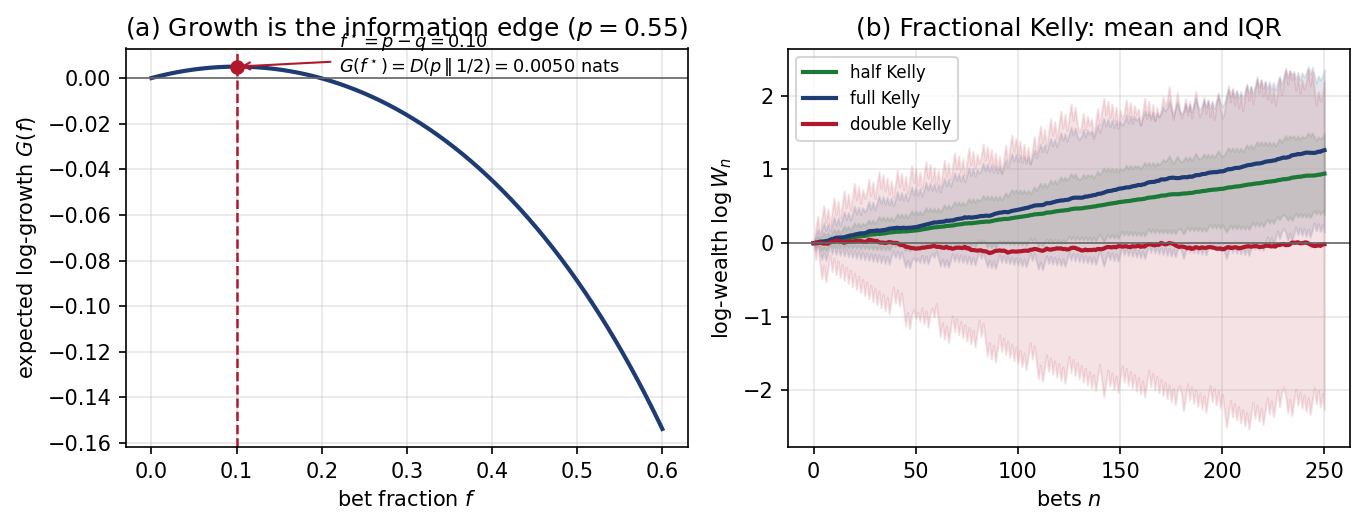
\includegraphics[width=\textwidth]{fig_kelly}
\caption{\small (a) Expected log-growth $G(f)$ for the even-money coin of Example~\ref{ex:coin}; the
optimum sits at $f^\star=p-q$ and equals $\D{\mathrm{Ber}(p)}{\mathrm{Ber}(1/2)}$, the information
edge. (b) Simulated log-wealth (mean and interquartile band, $400$ paths) at half, full, and double
Kelly. Full Kelly maximizes growth; half Kelly gives up little growth for much less variance; double
Kelly has essentially zero growth ($-0.00014$ nats/bet) despite betting more, illustrating why
overbetting is the cardinal sin and why fractional Kelly is prudent.}
\label{fig:kelly}
\end{figure}

\paragraph{Fractional Kelly and the penalty for overbetting.}
The growth curve $G(f)$ is concave with $G(0)=0$ and a second zero at $f=2f^\star$ in the symmetric
approximation: betting \emph{double} the Kelly fraction throws away the entire edge. For the coin of
Example~\ref{ex:coin}, $G(2f^\star)=-0.00014\approx 0$ nats. This asymmetry, that overbetting is
punished far more than underbetting, is the practical case for \emph{fractional} Kelly, betting
$\alpha f^\star$ with $\alpha<1$. Figure~\ref{fig:kelly}(b) shows the trade-off: half Kelly sacrifices
a quarter of the growth and cuts the log-variance to roughly a quarter. Section~\ref{sec:bayeskelly}
derives the right $\alpha$ from parameter uncertainty rather than taste.

\subsection{Thorp: blackjack as sequential Bayesian updating}\label{sec:thorp}
The archetype of a favorable game engineered by information is Thorp's strategy for twenty-one.
Blackjack is dealt \emph{without replacement}, so the conditional law of the next cards given those
already seen is a sequential Bayesian update. This is the sampling-without-replacement
structure of Section~\ref{ch:types}: conditioned on the cards played, the remaining deck is a finite population,
and the hypergeometric block law of the coupling of Section~\ref{ch:types} is the exact predictive object, close to the
i.i.d.\ law of the residual deck up to the collision term $m(m-1)/(2N)$ for $m$ cards from a deck of $N$. Card counting is nothing more
than tracking the sufficient statistic of that update, the composition of the residual deck; when the
update tilts the conditional expectation of the next hand in the player's favor, the growth rate of the Kelly bet
turns positive (it is the divergence $\D{p}{q}$ of Proposition~\ref{prop:kelly} only at fair odds, which the house does not offer), and the Kelly fraction, which increases with the player's expected gain,
scales the bet up.

Thorp's contribution was twofold: to show that such favorable situations arise with positive
frequency, and to size the bets by the growth criterion rather than by intuition. He then carried the
same logic from the table to the market, where the ``count'' becomes a statistical signal and the
bet becomes a portfolio weight. Breiman had already proved that the growth-optimal rule maximizes the
asymptotic growth rate and minimizes the expected time to reach a distant wealth goal (extended to arbitrary random returns by Finkelstein and Whitley, 1981); Bell, Cover,
and Algoet established the competitive and asymptotic optimality that make log-optimal investment
canonical rather than merely one utility among many. Samuelson's (1971) well-known objection, that maximizing
the geometric mean is not expected-utility optimal at a fixed finite horizon, concerns the utility,
which Section~\ref{sec:bayeskelly} keeps logarithmic; that section shows instead that once parameter uncertainty is admitted, the growth-optimal fraction is
automatically shrunk, and fractional Kelly emerges as the Bayesian, not the ad hoc, prescription.

\subsection{The log-optimal portfolio and Cover's universal portfolio}\label{sec:cover}
Move from a single bet to a market of $d$ assets. On day $t$ the price-relative vector is
$x_t\in\R^d_{+}$, $x_t(j)$ being the ratio of tomorrow's to today's price of asset $j$. A
\emph{constant rebalanced portfolio} (CRP) with weights $b$ in the simplex $\Delta_{d-1}$ reinvests
to hold those weights each day, earning
\[
S_n(b)=\prod_{t=1}^n \langle b,x_t\rangle,\qquad
\frac1n\log S_n(b)=\frac1n\sum_{t=1}^n\log\langle b,x_t\rangle.
\]
If the $x_t$ are i.i.d.\ with known law, the growth-rate-maximizing $b$ is the \emph{log-optimal}
portfolio, the direct analogue of Kelly's $b^\star=p$. In practice the law is unknown, and the target
is set retrospectively: the \emph{best CRP in hindsight} is $b^\star=\arg\max_b S_n(b)$, the
log-optimal portfolio of the realized empirical law. Cover's universal portfolio competes with it
with no model of the market at all.

\begin{theorem}[Cover; Cover and Ordentlich]\label{thm:cover}
Let $\nu$ be a probability measure on $\Delta_{d-1}$ and define the wealth-weighted average portfolio
\[
\hat b_{t+1}=\frac{\int_{\Delta} b\,S_t(b)\,\nu(db)}{\int_{\Delta} S_t(b)\,\nu(db)},\qquad \hat b_1=\int b\,\nu(db).
\]
Its wealth equals the $\nu$-mixture of CRP wealths, $S_n(\hat b)=\int_\Delta S_n(b)\,\nu(db)$. For
$\nu=\mathrm{Dir}(\tfrac12,\dots,\tfrac12)$, uniformly over every path of positive price
relatives,
\[
\log\max_b S_n(b)-\log S_n(\hat b)\ \le\ \frac{d-1}{2}\log n+O(1),
\]
so the universal portfolio attains the exponential growth rate of the best retrospective CRP.
\end{theorem}

\begin{proof}[Proof sketch]
The wealth identity is Fubini: $S_n(\hat b)$ telescopes to $\int S_n(b)\,\nu(db)$ because each day's
wealth-weighted average portfolio reinvests the mixture. For the regret, write
$S_n(b)=\exp\{n\,\bar\ell_n(b)\}$ with $\bar\ell_n(b)=\frac1n\sum_t\log\langle b,x_t\rangle$ concave in $b$
and maximized at $b^\star$. A Laplace expansion of $\int e^{n\bar\ell_n(b)}\nu(db)$ around an interior
maximizer with nondegenerate Hessian gives
\[
\int_\Delta e^{n\bar\ell_n(b)}\nu(db)=e^{n\bar\ell_n(b^\star)}\Big(\tfrac{2\pi}{n}\Big)^{(d-1)/2}
\frac{\nu'(b^\star)}{\sqrt{\det(-\nabla^2\bar\ell_n(b^\star))}}\,(1+o(1)),
\]
so $\log\max_b S_n-\log S_n(\hat b)=\frac{d-1}{2}\log n+O(1)$. The Dirichlet$(\tfrac12)$ density is
the Jeffreys prior on the simplex, whose $b^{-1/2}$ singularities at the boundary control the case of
a maximizer on a face and deliver the minimax constant; this is why Cover and Ordentlich single it
out. Their bound is uniform: expanding $S_n(b)=\prod_t\langle b,x_t\rangle$ as a sum over sequences of asset indices turns the wealth ratio into a ratio of coding probabilities, and the Krichevsky--Trofimov mixture gives, for every path of positive price relatives,
\[
\frac{\max_b S_n(b)}{S_n(\hat b)}\ \le\ \frac{\Gamma(\tfrac12)\,\Gamma(n+\tfrac d2)}{\Gamma(\tfrac d2)\,\Gamma(n+\tfrac12)}\ \le\ 2(n+1)^{(d-1)/2}.
\]
\end{proof}

\begin{figure}[H]
\centering
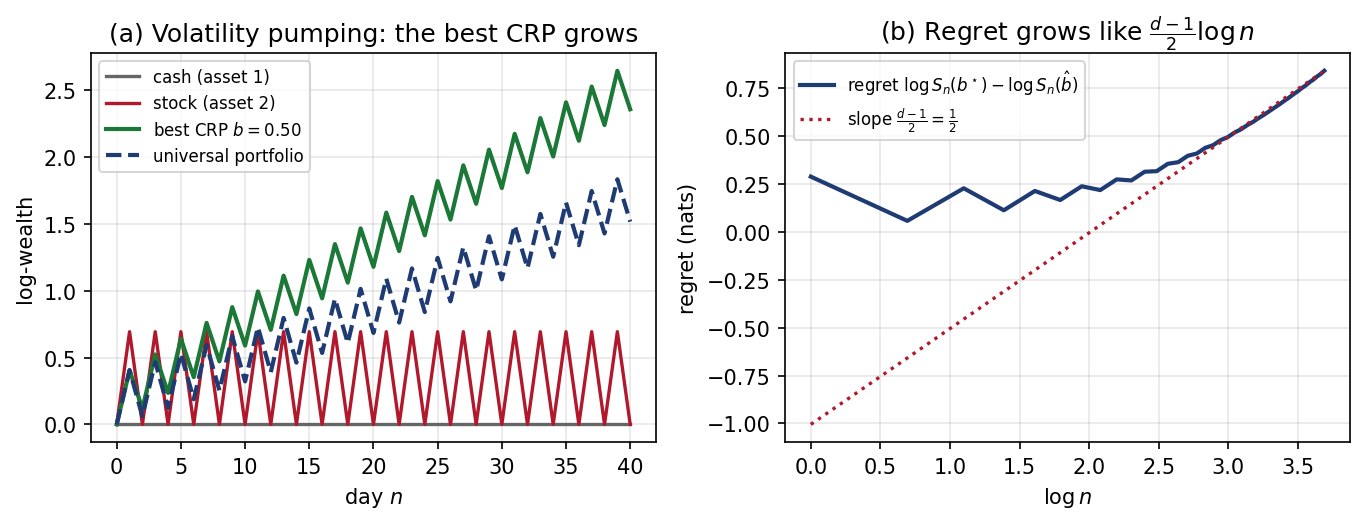
\includegraphics[width=\textwidth]{fig_universal}
\caption{\small Cover's ``volatility pumping'' market: asset~1 is cash and asset~2 alternates
price relatives $2$ and $\tfrac12$. (a) Both individual assets are flat (log-wealth $0$), yet the
best CRP $b^\star\approx(0.50,0.50)$ grows steadily, harvesting volatility; the universal portfolio,
using no model, tracks it. (b) The regret $\log S_n(b^\star)-\log S_n(\hat b)$ against $\log n$ grows
along the reference line of slope $\tfrac{d-1}{2}=\tfrac12$, as Proposition~\ref{prop:redundancy} predicts for this interior maximizer.}
\label{fig:universal}
\end{figure}

\begin{example}[Volatility pumping, in numbers]\label{ex:volpump}
Let asset~1 be cash ($x_t(1)=1$) and asset~2 alternate $x_t(2)\in\{2,\tfrac12\}$. Buy-and-hold of
either asset is flat: cash is constant, and the stock doubles then halves, netting $1$ every two
days, so both have log-wealth $0$ over an even horizon. The equal-weight CRP $b=(\tfrac12,\tfrac12)$
multiplies wealth by $\tfrac12(1)+\tfrac12(2)=1.5$ on up days and $\tfrac12(1)+\tfrac12(\tfrac12)=0.75$
on down days, hence by $1.125$ every two days: it \emph{grows} at $\tfrac12\log 1.125\approx 0.059$
per day out of pure volatility. Over $n=40$ days the best CRP reaches log-wealth $2.356$ while cash
and stock sit at $0$; the Dirichlet$(\tfrac12)$ universal portfolio reaches $1.513$, a regret of
$0.842$ nats (the $4000$ node grid used for the figure gives $1.516$ and
$0.840$), consistent with $\tfrac12\log n=\tfrac12\log 40\approx 1.84$ up to the $O(1)$ constant.
Figure~\ref{fig:universal} shows both panels.
\end{example}

\subsection{Universal portfolios are Bayes mixtures}\label{sec:upbayes}
The wealth identity $S_n(\hat b)=\int_\Delta S_n(b)\,\nu(db)$ is the reason the universal portfolio
belongs to this book. Read $S_t(b)=\prod_{s\le t}\langle b,x_s\rangle$ as a likelihood for the
portfolio weight $b$: the accumulated log-wealth is a log-likelihood, and the wealth-weighted average
$\hat b_{t+1}$ is the posterior mean of $b$ under prior $\nu$ and this likelihood. The
universal portfolio is the \emph{Bayes predictive portfolio}, a de Finetti mixture over CRPs, and
``universality'' is a redundancy statement.

\begin{proposition}[Universal portfolio as Bayesian redundancy]\label{prop:redundancy}
With $\nu$ as prior and $S_t(b)$ as likelihood, $\hat b_{t+1}=\E_\nu[b\mid x_{1:t}]$ is the posterior
mean, and, under the conditions of Theorem~\ref{thm:cover}, the regret is the Bayesian redundancy
\[
\begin{aligned}
\log\max_b S_n(b)-\log\!\int_\Delta S_n(b)\,\nu(db)
&=\underbrace{\log S_n(b^\star)-\log\text{(Bayes mixture)}}_{\text{redundancy}}\\
&\le\frac{d-1}{2}\log n+O(1).
\end{aligned}
\]
The bound is attained up to $O(1)$ in the Laplace case of the proof of Theorem~\ref{thm:cover}, when $b^\star$ stays in a compact subset of the interior of $\Delta_{d-1}$ and the eigenvalues of $-\nabla^2\bar\ell_n(b^\star)$ stay bounded away from $0$; it is not attained in general, since on the market with $x_t=(1,1)$ for all $t$ every CRP earns $1$ and the regret is $0$.
\end{proposition}

The $\tfrac{d-1}{2}\log n$ is the object that recurs throughout the book. It is the polynomial prefactor from the type
count of Section~\ref{ch:types}, of sharp order $N^{-(k-1)/2}$ for $k=d$ outcomes (the bound $(N+1)^{-k}$ there is cruder), discarded there; it is the Schwarz identity of
Section~\ref{ch:risk}, where $\tfrac12\log n$ per parameter is what a fixed $p$-value threshold
declines to pay; and it is the genome-wide threshold's $\tfrac12\log(m^2n)$ inflation. Universal
portfolios are therefore the finance instance of one redundancy theory: the price of not knowing the
best model in advance is half a $\log n$ per free parameter, whether the model is a directing measure,
a null hypothesis, or a portfolio. Cover and Ordentlich's extension with side information, in which
the CRP is allowed to depend on an observed state, is the finance instance of conditioning the mixing
measure, the constraint posterior of Section~\ref{ch:projected}: universality with side information is universality of
the \emph{conditional} Bayes mixture. The growth theory of investment and the redundancy theory of
Bayesian prediction are one subject.

\subsection{Bayesian asset allocation}\label{sec:bayeskelly}
When the return law is estimated rather than known, the log-optimal weights inherit estimation error,
and substituting point estimates into the optimizer is provably suboptimal. The remedy, due to Zellner
and Chetty (1965) and developed for finance by Jacquier and Polson, is to maximize expected utility under the
\emph{predictive} return density
\[
p(r_{T+1}\mid \text{data})=\int p(r_{T+1}\mid\theta)\,\pi(\theta\mid\text{data})\,d\theta,
\]
the essentially Bayesian object of Chapter~\ref{chap:prediction}. The investor solves
$\max_f \E_{\text{pred}}[\log(1+f^\top r_{T+1})]$, integrating over parameter uncertainty rather than
conditioning on a point estimate.

Three consequences follow. First, the predictive variance exceeds the plug-in variance, so the
Bayesian optimal portfolio takes \emph{smaller} positions in high-estimated-return, high-risk assets;
the effect grows with the number of assets relative to the sample length, and it is the portfolio
face of the James--Stein and horseshoe shrinkage developed elsewhere in the book, and of Jorion's
Bayes--Stein allocation. Second, fractional Kelly is \emph{Bayesian} Kelly: parameter uncertainty
inflates the predictive dispersion and fattens its tails, and because $\log(1+fr)$ is severely
sensitive to large losses, the growth-optimal fraction is scaled below full Kelly, by more when the
sample is short. The practitioner's half-Kelly is the posterior-predictive Kelly, not a superstition.
Third, computation is generative: the predictive density and its expected-utility functionals are
obtained by Markov chain Monte Carlo and particle filtering, as in the Bayesian stochastic volatility\index{stochastic volatility}
models of Jacquier, Polson, and Rossi, which is the generative Bayesian computation of the book
applied to returns.

\begin{remark}[Fractional Kelly from estimation risk]\label{prop:fractional}
Let monthly returns be $r_t\mid\mu\sim\mathcal N(\mu,\sigma^2)$ with a diffuse prior on $(\mu,\sigma)$,
so the predictive law after $T$ observations is location-scale Student-$t$ with $T-1$ degrees of
freedom, location $\hat m$, and scale $\hat\sigma\sqrt{1+1/T}$. For $\hat m=0.008$ and $\hat\sigma=0.045$ (Figure~\ref{fig:bayeskelly}), the computed Bayesian growth-optimal fraction
$f_{\mathrm{Bayes}}(T)=\arg\max_{0\le f\le 20} \E_{\text{pred}}[\log(1+f r)]$ increases with $T$ for every sample size $T$ from $6$ to $600$, stays strictly
below the plug-in Kelly fraction $f_{\mathrm{plug}}=\arg\max_{0\le f\le 20} \E_{\mathcal N(\hat m,\hat\sigma^2)}[\log(1+fr)]$,
and approaches it as $T$ grows. Throughout, $\log(1+f r)$ is floored at $\log 10^{-9}$ for both predictives,
so that an outcome with $1+f r\le 0$ costs a finite loss and the expected log-growth is finite; without the
floor the unbounded predictive assigns positive probability to $1+f r\le 0$ and
$\E_{\text{pred}}[\log(1+f r)]$ diverges. The cap $f\le 20$ is part of the definition, because the floored objective grows like $\log f$ as $f\to\infty$.
\end{remark}

\begin{figure}[H]
\centering
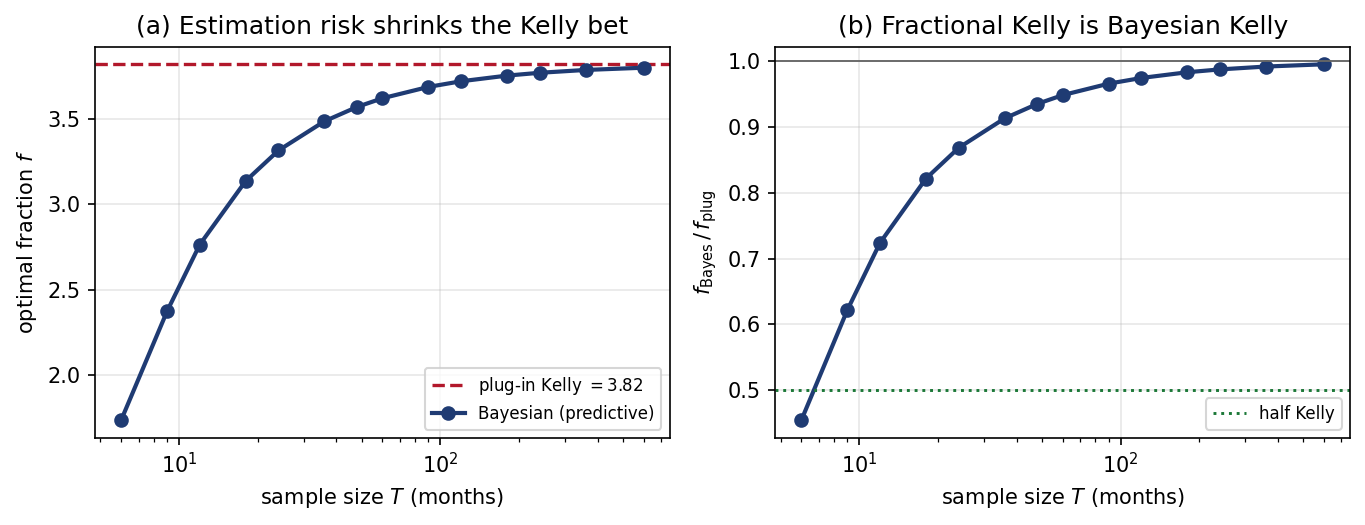
\includegraphics[width=\textwidth]{fig_bayeskelly}
\caption{\small Bayesian asset allocation for one risky asset ($\hat m=0.008$, $\hat\sigma=0.045$
monthly). (a) The plug-in Kelly fraction ($3.82$) ignores estimation error; the Bayesian fraction,
computed under a Student-$t$ predictive, is materially smaller for short samples and rises toward the
plug-in value as data accumulate. (b) The ratio $f_{\mathrm{Bayes}}/f_{\mathrm{plug}}$: about $0.72$
at $T=12$ months and $0.95$ at $T=60$, so ``fractional Kelly'' is what a Bayesian who accounts for
parameter uncertainty does automatically. Fractions maximize the expected log-growth over $0\le f\le 20$ with $\log(1+fr)$ floored at $\log 10^{-9}$ (Remark~\ref{prop:fractional}).}
\label{fig:bayeskelly}
\end{figure}

\begin{example}[How much to shrink, in numbers]\label{ex:shrink}
With $\hat m=0.008$ and $\hat\sigma=0.045$ per month, the plug-in Kelly fraction is
$f_{\mathrm{plug}}=3.82$ (a heavily levered position, as pure Kelly on a single asset usually is).
Under the Student-$t$ predictive, with the floor of Remark~\ref{prop:fractional}, $f_{\mathrm{Bayes}}=2.77$ at $T=12$ months, a ratio of $0.72$, and
the ratio rises to $0.95$ by $T=60$. A five-year record buys most of the way to full Kelly; a single
year justifies roughly three-quarter Kelly. Figure~\ref{fig:bayeskelly} shows the whole curve. The
shrinkage is not imposed; it falls out of integrating the growth objective over the posterior, and it
is the same mechanism, predictive-variance inflation, that shrinks the mean-variance weights in
Jacquier and Polson.
\end{example}

\subsection{Rational inattention in portfolio choice}\label{sec:ri}
The economics of Section~\ref{ch:er} apply directly to how an investor allocates \emph{attention} rather than
capital. An agent with a finite Shannon capacity $\kappa$ chooses which return signals to track,
solving a rate--distortion problem whose solution is reverse water-filling: attention is spent on the
high-variance factors first, and factors below the water level receive exactly zero nats. Assets whose
idiosyncratic risk falls under the level are not tracked imprecisely; they are not tracked at all,
and they drop out of the consideration set, the active-set phenomenon of Section~\ref{ch:er}. This yields an
information-theoretic account of under-diversification and home bias: an investor with a limited
attention budget rationally concentrates on a few salient factors and ignores the rest, and the
cutoff is the shadow price of a nat. Rational inattention thus closes the loop between the
entropy-regularized prediction of Section~\ref{ch:er} and the growth-optimal investment of this section: the
first says which signals are worth tracking, the second says how to bet once they are.

\subsection{One object}\label{sec:oneobject}
Kelly growth is the log score, which is a Kullback--Leibler edge (Proposition~\ref{prop:kelly}); the
universal portfolio is a Bayes mixture whose regret is at most the $\tfrac{d-1}{2}\log n$ redundancy of the
method of types and the Schwarz threshold (Theorem~\ref{thm:cover},
Proposition~\ref{prop:redundancy}); Bayesian asset allocation is predictive expected-utility
maximization, with fractional Kelly as its automatic shrinkage (Remark~\ref{prop:fractional});
and rational inattention is rate--distortion, deciding which signals earn capacity. Each is the book's
thesis read as investment: prediction scored by log-loss, mixed over a prior, under an information
budget. The finance section is not an application bolted onto a statistics book; it is the same
predictive, information-theoretic construction, wearing the clothes of a portfolio.

\subsection*{Problems}
\begin{enumerate}[leftmargin=2.2em,itemsep=2pt]
\item For an even money bet won with probability $p>\tfrac12$, show that the growth rate of betting the
fraction $f$ is $p\log(1+f)+(1-p)\log(1-f)$, maximized at $f=2p-1$ with value $\log2-H(p)=
\D{\mathrm{Ber}(p)}{\mathrm{Ber}(\tfrac12)}$.
\item Show that betting $c$ times the Kelly fraction gives, to second order, the fraction $c(2-c)$ of
the optimal growth, so that twice Kelly has zero growth.
\item A stock doubles or halves with equal probability each period. Show that holding it alone has
zero growth, while rebalancing to half stock and half cash grows at $\tfrac12\log1.125$ per period.
\item With a normal posterior of mean $m$ and variance $v$ for the excess drift, show that the log
optimal fraction is, to leading order, $m/(\sigma^2+v)$, the rule \eqref{up:eq:bayeskelly} (compare Remark~\ref{prop:fractional}).
\item Model the true count in blackjack as a sufficient statistic for the composition of the remaining
shoe, and show that betting proportional to the posterior edge is the Kelly rule of
Section~\ref{sec:thorp}.
\item Show that Cover's universal portfolio is the posterior mean under a prior on constant rebalanced
portfolios (Proposition~\ref{prop:redundancy}), and compare with Section~\ref{ch:upbayes}.
\end{enumerate}

\src{Kelly (1956); Thorp (1961, 1969, 2006); Rotando and Thorp (1992); Breiman (1961); Bell and Cover
(1980); Algoet and Cover (1988); Cover (1991); Cover and Ordentlich (1996); Browne and Whitt (1996);
Jorion (1986); Jacquier, Polson, and Rossi (1994); Jacquier and Polson (2013); and the
entropy-regularized prediction of Section~\ref{ch:er}.}

%====================================================================================================


\section[Universal Portfolio as a Bayes Rule]{Worked Example: Cover's Universal Portfolio as a Bayes Rule}\label{ch:upbayes}
\index{universal portfolio}\index{Kelly criterion}\index{Jeffreys prior}\index{fractional Kelly}\index{Parrondo's paradox}\index{roulette}

Section~\ref{sec:upbayes} observed that Cover's universal portfolio is a Bayes mixture. This section
takes that observation literally and works it through as a single extended example: the wealth of a
constant rebalanced portfolio is a likelihood for the weights, the universal portfolio is the
posterior mean, its wealth is the marginal likelihood, and its regret is a log Bayes factor. Everything
the book has developed about evidence, Laplace expansions, Jeffreys priors, Bernstein--von Mises
concentration and shrinkage then applies verbatim, and it explains rather than merely reproduces the
known guarantees. The example ends with real data: a pair of losing stocks that combine into a
winner, one hundred and fifty two years of the SP500, Thorp's Berkshire Hathaway calculation, and the
four hundred and seventy constituents of the index with a complete five year history.

Throughout, a market over $d$ assets is a sequence of price relatives $x_1,x_2,\dots\in\R^d_+$, a
portfolio is a point $b$ of the simplex $\Delta$ of dimension $d-1$, and the constant rebalanced
portfolio $b$ has wealth after $T$ periods
\begin{equation}\label{up:eq:wealth}
S_T(b)=\prod_{t=1}^T b^\top x_t,\qquad \ell_T(b)=\log S_T(b),
\end{equation}
which is concave in $b$, so the hindsight optimum $\tilde b_T=\argmax_b\ell_T(b)$ exists and is
computable by Cover's fixed point iteration (Cover, 1984). A causal strategy $\hat b_t$, measurable with respect to
$\mathcal F_{t-1}=\sigma(x_1,\dots,x_{t-1})$, earns $\hat S_T=\prod_t\hat b_t^\top x_t$, and its regret is
$R_T=\log S_T(\tilde b_T)-\log\hat S_T$.

\subsection{Wealth is evidence}
Fix a prior $\Pi$ on $\Delta$ with density $\pi$, treat \eqref{up:eq:wealth} as a likelihood for $b$,
and define the posterior and its mean,
\begin{equation}\label{up:eq:post}
\pi_t(db)=\frac{S_t(b)\,\Pi(db)}{\int_\Delta S_t(b)\,\Pi(db)},\qquad
\hat b_{t+1}=\E_{\pi_t}[b]=\frac{\int_\Delta b\,S_t(b)\,\Pi(db)}{\int_\Delta S_t(b)\,\Pi(db)}.
\end{equation}
The second display is Cover's rule of Theorem~\ref{thm:cover}. In a general market $b\mapsto S_t(b)$ is
a pseudo likelihood rather than a density in $x$, so \eqref{up:eq:post} is a Gibbs posterior in the
sense of Bissiri, Holmes and Walker, with loss the negative log wealth and learning rate one. The rate
is not free: it is pinned at one by the requirement that the normalizer be interpretable as money.
The update reweights the prior by money, so a portfolio's posterior mass is its prior mass times the
wealth it would have made, with no tuning constant anywhere.

\begin{theorem}[Wealth is evidence]\label{up:thm:evidence}
Let $m_t=\int_\Delta S_t(b)\,\Pi(db)$ with $m_0=1$. For every price sequence and every prior,
$\hat S_T=m_T$.
\end{theorem}

\begin{proof}
The one period relative $b\mapsto b^\top x_t$ is linear, so
$m_t/m_{t-1}=\E_{\pi_{t-1}}[b^\top x_t]=(\E_{\pi_{t-1}}[b])^\top x_t=\hat b_t^\top x_t$. Multiply over
$t$ and telescope.
\end{proof}

\begin{corollary}[Regret is a log Bayes factor]\label{up:cor:bf}
$R_T=\log\{\sup_b S_T(b)/m_T\}$, the log ratio of the maximized likelihood to the marginal
likelihood, which is the redundancy, or stochastic complexity, of universal coding.
\end{corollary}

Two remarks keep the reading honest. The universal portfolio is Bayesian model averaging in which the
models are the constant rebalanced portfolios and the quantity averaged is money; the linearity that
makes averaging money the same as averaging weights is what fails for nonlinear utility.
And the posterior mean is not the myopic Bayes rule $\argmax_b\E[\log b^\top x_{t+1}\mid\mathcal
F_t]$: the two differ by a Jensen gap of order $\|b-b^\star\|^2$ and agree only asymptotically. The
posterior mean is preferred because it alone reproduces the evidence path by path, which is what turns
a Bayesian statement into a guarantee for every sequence.

\paragraph{The horse race market.} If exactly one asset pays in each period, $x_t=O_t e_{j_t}$, then
$S_T(b)=(\prod_tO_t)\prod_jb_j^{n_{T,j}}$ with $n_{T,j}$ the number of wins of asset $j$. The wealth
is now a genuine multinomial likelihood and the Dirichlet prior $\mathrm{Dir}(\alpha_1,\dots,\alpha_d)$
is conjugate:
\begin{equation}\label{up:eq:shrink}
\hat b_{t+1,j}=\frac{\alpha_j+n_{t,j}}{\alpha_0+t}
=\frac{t}{t+\alpha_0}\,\frac{n_{t,j}}{t}+\frac{\alpha_0}{t+\alpha_0}\,\frac{\alpha_j}{\alpha_0},
\qquad\alpha_0=\textstyle\sum_j\alpha_j .
\end{equation}
With $\alpha_j\equiv\frac12$ this is the Krichevsky and Trofimov add one half rule, and the Dirichlet
multinomial evidence is the de Finetti representation of an exchangeable market. The universal
portfolio never plays the plug in Kelly rule $n_t/t$; it plays a shrunk version of it, with a
shrinkage weight $\alpha_0/(t+\alpha_0)$ that vanishes at rate $1/t$.

\subsection{Asymptotics for free}
Assume a stationary ergodic market with a unique interior maximizer $b^\star$ of the growth rate
$W(b)=\E\log b^\top x$, relatives bounded away from zero and infinity, and write
$\Info(b)=\E[xx^\top/(b^\top x)^2]$ for the market information matrix on the tangent space of the simplex.
The Laplace expansion of $m_T$ gives the following, stated without a formal proof; for the uniform prior its first display recovers the asymptotic of Cover (1991).

\begin{theorem}[Regret expansion]\label{up:thm:regret}
Under these conditions, almost surely,
\[
R_T=\frac{d-1}2\log\frac{T}{2\pi}+\frac12\log\det\Info(b^\star)-\log\pi(b^\star)+o(1).
\]
Suppose further that the market is one of a family indexed by the growth optimal portfolio, and read $\Info(b)$ as the information of the member whose growth optimal portfolio is $b$, which at $b=b^\star$ is the information above.
If $\pi$ is the Jeffreys prior $\pi_J(b)\propto\sqrt{\det\Info(b)}$ with finite volume
$C=\int_\Delta\sqrt{\det\Info(b)}\,db$, then $R_T=\frac{d-1}2\log\frac T{2\pi}+\log C+o(1)$, which does not
depend on $b^\star$.
\end{theorem}

This is the Rissanen and Shtarkov expansion of stochastic complexity transplanted to portfolios, and
the last display is the equalizer property behind the minimaxity of Clarke and Barron. In the horse
race with win probabilities $p$, $\Info(b)=\diag(p_j/b_j^2)$, which is $\diag(1/b_j)$ only at $b=b^\star=p$; the race whose growth optimal portfolio is $b$ has win probabilities $b$, so in the reading of the theorem $\Info(b)=\diag(1/b_j)$ and the Jeffreys prior is $\mathrm{Dir}(\frac12,\dots,\frac12)$: the
Cover and Ordentlich prior is not a tuning choice but the reference prior of the model the market
defines. Its volume is $C=\Gamma(\frac12)^d/\Gamma(\frac d2)$. The zero relatives put the horse race outside the conditions of the theorem, but Stirling's formula applied to its Dirichlet multinomial evidence gives the asymptotic regret
$\frac{d-1}2\log\frac T{2\pi}+\frac d2\log\pi-\log\Gamma(\frac d2)+o(1)$ directly, on every path on which each count $n_{T,j}$ grows without bound. Against the Cover and Ordentlich
bound
\begin{equation}\label{up:eq:co}
\log\frac{S_T(\tilde b_T)}{\hat S_T}\le\log2+\frac{d-1}2\log(T+1),
\end{equation}
valid for every sequence, the two numbers are $4.48$ and $4.95$ for two assets at $T=5000$, and $121.7$
and $171.1$ for thirty eight pockets at $T=10\,000$. The bound is loose by a factor growing with
dimension, which will matter below.

Bernstein--von Mises supplies the rest. The posterior satisfies
$\pi_t(\sqrt t(b-\hat b_t)\in\cdot)\to\mathcal N(0,\Info(b^\star)^{-1})$, so the weights are learned at the
parametric rate, and since $\nabla W(b^\star)=0$ on the simplex the expected one period shortfall is
$\frac12\tr(\Info(b^\star)\operatorname{Var}\hat b_{t+1})=(d-1)/(2t)+o(1/t)$, whose partial sums are the
$\frac{d-1}2\log T$ of Theorem~\ref{up:thm:regret}. The logarithmic regret is the accumulated cost of
learning $d-1$ parameters at rate $1/t$ each. When $b^\star$ lies on a face the expansion above does not apply, because the limit is not Gaussian in
the directions normal to the face.

\subsection{Computation: the normalizer is the money}
Take interior nodes $b^{(1)},\dots,b^{(N)}$ with prior weights $q_k\propto\pi(b^{(k)})\Delta_k$, where $\Delta_k$ is the volume of the grid cell containing $b^{(k)}$. Since
Theorem~\ref{up:thm:evidence} holds for every prior, a grid is not an approximation to a universal
portfolio: it is the universal portfolio of the discrete prior $\sum_kq_k\delta_{b^{(k)}}$. The
recursion is a fixed node filter with a multiplicative update: hold $\hat b_t=\sum_kw_kb^{(k)}$,
observe $x_t$, set $v_k=w_k\,b^{(k)\top}x_t$, $Z_t=\sum_kv_k$, $w_k\leftarrow v_k/Z_t$.

\begin{proposition}[The normalizer is the money]\label{up:prop:grid}
$Z_t=\hat b_t^\top x_t$, hence $\hat S_T=\prod_tZ_t=\sum_kq_kS_T(b^{(k)})$.
\end{proposition}

The constant a filter usually throws away is here the period's return, so the algorithm returns the
bank balance as a byproduct of renormalizing. There are no logarithms or exponentials, only one
multiplication and one sum per node per period, and renormalizing removes the underflow that direct
evaluation of $S_t(b)$ invites. For $\alpha_j<1$ the Dirichlet density is singular on the faces, so
nodes are cell midpoints; near a vertex, the normal situation in gambling where most wealth is held
in reserve, the roulette example below grades the cell edges as $(i/N)^3$. On the Parrondo path below
the terminal log wealth falls monotonically from $1.096$ with $11$ nodes to $0.991$ with $4001$ and
$0.989$ with $16\,001$, while the terminal posterior mean settles at $0.471$ by $N\approx400$. A
coarse grid is not a numerical error: every row is a wealth actually attainable by the rule of that
discrete prior.

\subsection{A Parrondo market}
Take two assets with independent relatives $1\pm f$, probability $p$ of the upward move, $p=0.51$ and
$f=0.05$. Each asset has positive expected return $1.001$ but negative growth rate,
$p\log(1+f)+(1-p)\log(1-f)=-2.507\times10^{-4}$, so each alone loses money almost surely. The equal
weight portfolio has growth rate $p^2\log(1+f)+(1-p)^2\log(1-f)=+3.748\times10^{-4}$, because the
mixed outcome, which has probability about one half, returns exactly one and removes half the
variance. Two losing bets combine into a winner: this is volatility pumping, the portfolio form of
Parrondo's paradox, and $b^\star=(\frac12,\frac12)$. The market information at $b^\star$ in the free
coordinate $\omega=b_1$ is $\Info=2p(1-p)(2f)^2=4.998\times10^{-3}$, so the posterior standard deviation
at $T=5000$ is about $(T\Info)^{-1/2}=0.20$: the growth surface is very flat, which is the regime
in which shrinkage matters.

\begin{table}[t]
\centering\small
\begin{tabular}{lrr}
\toprule
Strategy & $\log S_T$ & $S_T$\\
\midrule
Asset 1 alone & $-1.454$ & $0.234$\\
Asset 2 alone & $-0.853$ & $0.426$\\
Equal weight portfolio & $2.010$ & $7.466$\\
Best in hindsight, $\tilde\omega_T=0.476$ & $2.018$ & $7.520$\\
Universal portfolio (posterior mean) & $0.991$ & $2.695$\\
Marginal likelihood $\log m_T$ & $0.991$ & $2.695$\\
\midrule
Realized regret $R_T$ & $1.026$ & \\
Bound $\log2+\frac12\log(T+1)$ & $4.952$ & \\
\bottomrule
\end{tabular}
\caption{\small One simulated path of the Parrondo market, $T=5000$, $\mathrm{Beta}(\frac12,\frac12)$
prior, $4001$ grid nodes. The universal portfolio's wealth equals the marginal likelihood to
$1.7\times10^{-14}$, a numerical check of Theorem~\ref{up:thm:evidence}.}
\label{up:tab:path}
\end{table}

Table~\ref{up:tab:path} reports a path on which both assets lose money. Over $400$ independent paths
the median terminal log wealth is $-1.15$ for a single asset, $2.20$ for the equal weight portfolio,
$2.70$ for the hindsight optimum and $1.73$ for the universal portfolio; a single asset ends below its
start on $64$ percent of paths, the universal portfolio ends above it on $74$ percent, and the mean
regret is $0.98$ with a maximum of $1.36$ against the bound $4.95$. The Bernstein--von Mises scale is
visible directly: over $200$ further paths the average posterior standard deviation times $\sqrt T$ is
$14.0$ and the spread of the posterior mean across paths times $\sqrt T$ is $13.5$, against
$\Info^{-1/2}=14.1$. Figures~\ref{up:fig:wealth} to~\ref{up:fig:post} show the wealth paths, the inverted
bowl of terminal wealth against the weight, the regret against the bound, and the posterior mean with
a band contracting at rate $t^{-1/2}$.

\begin{figure}[H]
\centering
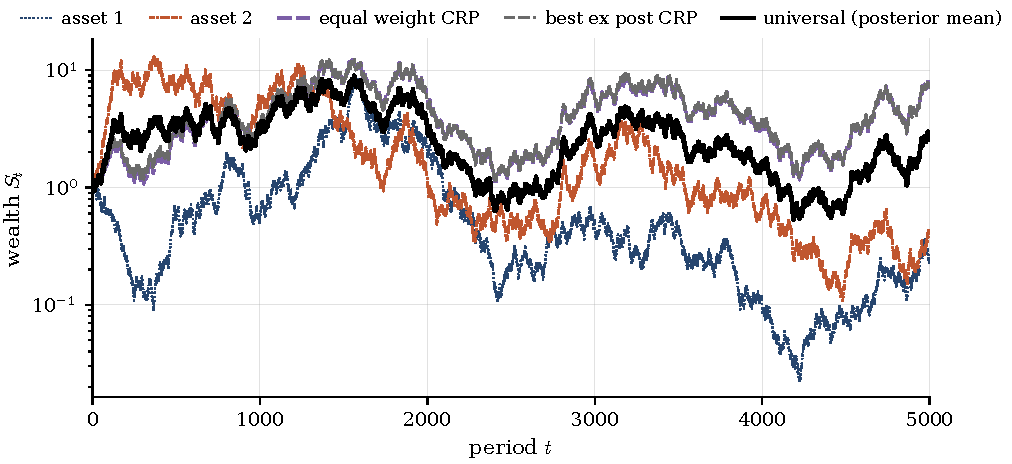
\includegraphics[width=0.88\textwidth]{up_fig_wealth}
\caption{\small Wealth on a log scale in the Parrondo market. Each asset alone loses money; the
rebalanced mixtures grow, and the universal portfolio, whose wealth is the marginal likelihood,
tracks the hindsight optimum with a gap growing only logarithmically.}
\label{up:fig:wealth}
\end{figure}

\begin{figure}[H]
\centering
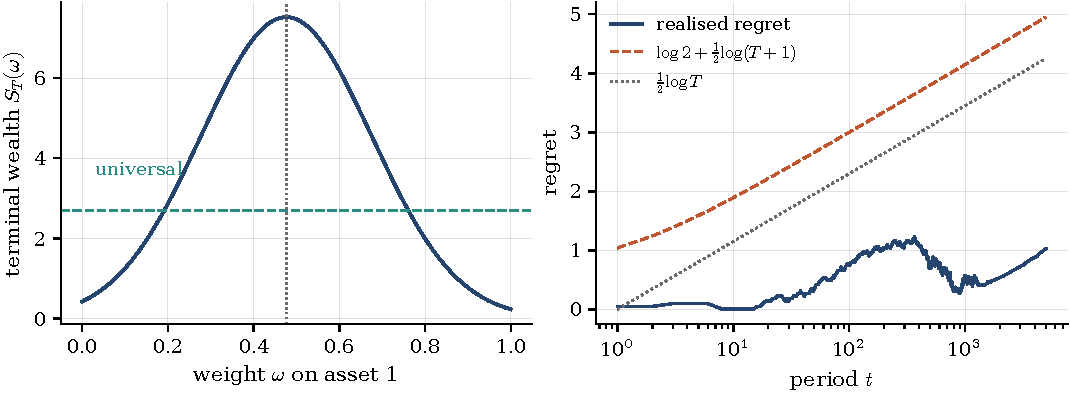
\includegraphics[width=\textwidth]{up_fig_regret}
\caption{\small Left: terminal wealth of the portfolio with weight $\omega$ on asset 1, with the
universal portfolio as a horizontal line and the hindsight optimum as a vertical line. Right: realized
regret against the Cover and Ordentlich bound and the rate $\frac12\log t$.}
\label{up:fig:regret}
\end{figure}

\begin{figure}[H]
\centering
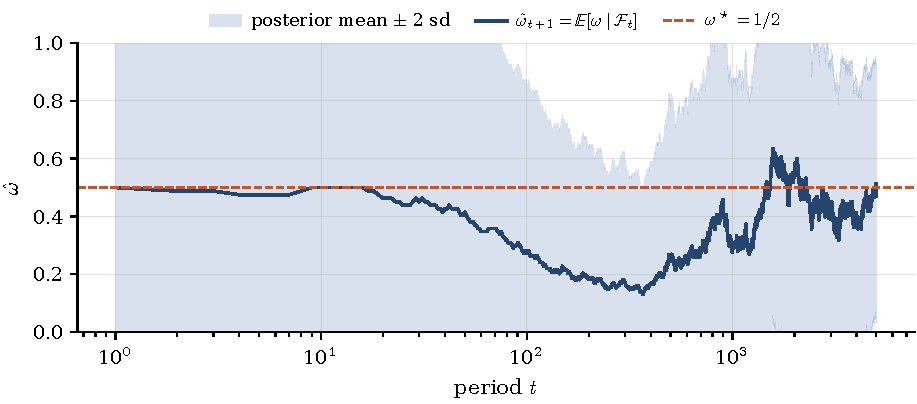
\includegraphics[width=0.88\textwidth]{up_fig_posterior}
\caption{\small Posterior mean weight $\hat\omega_{t+1}=\E[\omega\mid\mathcal F_t]$ with a two standard
deviation band. The band contracts at rate $t^{-1/2}$ with constant $\Info^{-1/2}=14.1$, and the mean
wanders inside it for a long time because $\Info$ is small.}
\label{up:fig:post}
\end{figure}

\paragraph{The same effect in the SP500.} The geometry is not artificial. In daily closing prices of
the SP500 constituents from February 2013 to February 2018, $T=1258$ days, Newmont Mining ended at
$0.824$ of its starting price and Williams Companies at $0.833$, while the daily rebalanced half and
half portfolio ended at $1.029$; their log returns are nearly uncorrelated. The hindsight weight is
$0.490$, the universal portfolio ends at $0.927$, and the realized regret is $0.104$ against a bound
of $4.26$ (Figure~\ref{up:fig:realpair}). The diagnostic worth more than the wealth is the posterior:
after five years of daily data its standard deviation is $0.343$, against a prior value of $0.354$.
The data have barely moved it. The information is $\Info=1.37\times10^{-3}$, so the Bernstein--von Mises
scale $\Info^{-1/2}=27.0$ is far above the observed $\sqrt T$ times the posterior standard deviation,
$12.2$, because the prior is still doing the work. The universal portfolio does well here not because
it has learned the weights but because the prior mean, one half, is nearly optimal. At equity
horizons the wealth surface is so flat that regret is small for the same reason learning is
negligible.

\begin{figure}[H]
\centering
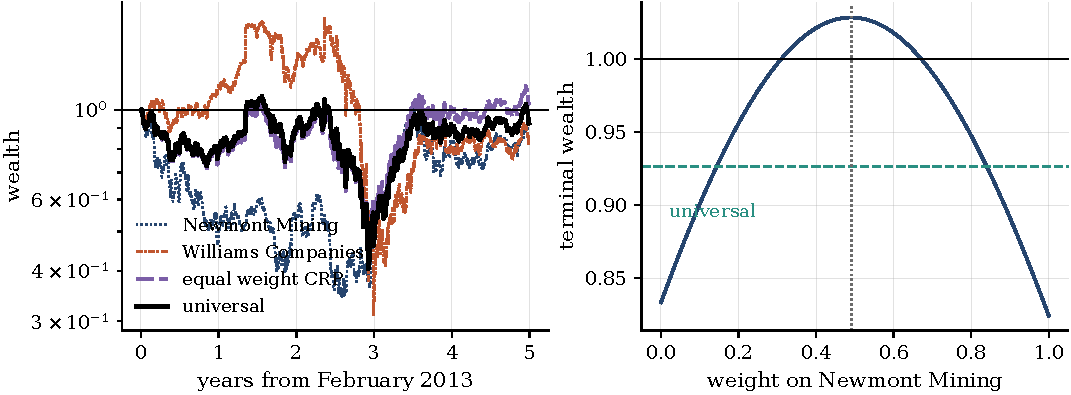
\includegraphics[width=\textwidth]{up_fig_realpair}
\caption{\small Two SP500 constituents that each lost about a sixth of their value over five years.
Left: wealth of each, of the daily rebalanced equal weight portfolio, and of the universal portfolio.
Right: terminal wealth against the weight on Newmont. Prices are unadjusted for dividends.}
\label{up:fig:realpair}
\end{figure}

\subsection{A biased roulette wheel}
On an American wheel with $38$ pockets every permitted bet returns at most $36/38$ of the stake in
expectation, so a true wheel is unbeatable and the only opening is a mechanical bias. The market is a
horse race with a cash reserve, and the log optimal rule is water filling.

\begin{proposition}[Kelly with a reserve]\label{up:prop:kelly}
Let outcome $j$ have probability $p_j$ and gross odds $o_j$, with unstaked wealth held as cash. For a
staked set $A$ put $P_A=\sum_{j\in A}p_j$ and $Q_A=\sum_{j\in A}1/o_j$. The log optimal allocation is
\[
b_0^\star=\frac{1-P_A}{1-Q_A},\qquad b_j^\star=p_j-\frac{b_0^\star}{o_j}\ (j\in A),\qquad b_j^\star=0\
(j\notin A),
\]
where $j\in A$ if and only if $p_jo_j>b_0^\star$, found by sorting on $p_jo_j$ and adding outcomes
while the condition holds. The growth rate is
$\sum_{j\in A}p_j\log(p_jo_j)+(1-P_A)\log b_0^\star$.
\end{proposition}

\begin{proof}[Sketch]
The first order conditions give $p_jo_j/(b_0+o_jb_j)=\lambda$ on $A$ and
$\sum_jp_j/(b_0+o_jb_j)=\lambda$ for cash; the budget constraint forces $\lambda=1$, so the wealth
relative on a staked outcome is $p_jo_j$, and outcomes with $p_jo_j\le b_0^\star$ have a negative
multiplier.
\end{proof}

This is the water filling structure of the horse race in Cover and Thomas, and of
Section~\ref{ch:er}. The classical alternative is a test. Ethier (1982) tests whether no pocket is
favorable, $H_0:\max_jp_j\le1/36$, and flags the most frequent number when its count exceeds
$n/36+a\sqrt n$, with $a\approx0.49$ at the five percent level. The centering is $1/36$, the break even
frequency at $35$ to $1$, and the inflated margin is the price of a maximum over $38$ pockets. The test
says whether to bet, not how much, and discards the shape of the count vector; a posterior mean fills
both gaps. A Bayes rule with a Dirichlet prior was studied by Klotz (2000), and a Bayesian remark is
already attributed to Kurtz in Ethier's 1982 paper.

Take a wheel on which two pockets come up with probability $1/30$ each and the other $36$ share the
rest, over $T=10\,000$ spins. Since $p_jo_j=1.2$ on the favored pair and $0.933$ elsewhere,
Proposition~\ref{up:prop:kelly} gives $b_0^\star=0.98824$, a stake of $0.00588$ on each favored pocket,
and growth rate $1.109\times10^{-3}$, so the whole edge is worth $11.09$ in log wealth over the
horizon. On the simulated path the screening rule raises a brief false alarm on an unfavored pocket
at spins $230$ to $234$, first fires on a favored pocket at spin $7694$, and fires at every $n$ from
spin $8558$ on; at the horizon the favored pockets show $333$ and $332$ hits against a critical value
of $326.8$, and the best of the rest shows $292$.

Run the universal portfolio on the three asset simplex of cash and the two screened pockets with a
graded grid of $79\,504$ nodes (Table~\ref{up:tab:roulette}, Figure~\ref{up:fig:roulette}). Three
lessons follow, all from the Bayesian reading rather than the bound. First, the prior mean is the
opening portfolio, so put it where you can afford to be wrong: the mean of
$\mathrm{Dir}(\frac12,\frac12,\frac12)$ stakes two thirds of wealth on two single numbers, the first
hundred spins cost $2.71$ in log wealth, and the loss is made up only late (log wealth is still $-2.48$ at spin $5000$). Moving prior mass to cash
is worth $3.5$ in terminal log wealth, a factor of thirty, without touching the leading term of the
guarantee; it is the $-\log\pi(b^\star)$ of Theorem~\ref{up:thm:regret} made concrete, and the only term
the investor controls. A pocket's relative is zero on every spin it loses, so the wheel is outside the conditions of the theorem as stated, but the Laplace expansion behind it needs the portfolio relative $b^\top x$ bounded away from zero only for $b$ near $b^\star$, and there cash keeps $b^\top x\ge b_0\approx0.99$. Second, screening is dimension reduction: over all $38$ pockets and cash the
bound reads $\log2+19\log(T+1)$, which falls below the available edge only after roughly two hundred
thousand spins. Third, conjugacy fails but the identity does not: with cash the relative
$b_0+o_jb_j$ is linear but not multinomial in $b$, so there is no closed form, which is why the grid
exists.

\begin{table}[t]
\centering\small
\begin{tabular}{lrrr}
\toprule
Strategy & $\log S_T$ & $S_T$ & regret\\
\midrule
Cash & $0.000$ & $1$ & \\
Universal, $\mathrm{Dir}(\frac12,\frac12,\frac12)$ & $3.422$ & $30.6$ & $7.35$\\
Universal, $\mathrm{Dir}(4,\frac12,\frac12)$ & $5.459$ & $235$ & $5.31$\\
Universal, $\mathrm{Dir}(20,\frac12,\frac12)$ & $6.893$ & $985$ & $3.88$\\
Kelly rule, bias known & $10.769$ & $47\,500$ & \\
Best in hindsight on the grid & $10.768$ & $47\,500$ & \\
Bound $\log2+\log(T+1)$ & & & $9.90$\\
\bottomrule
\end{tabular}
\caption{\small The biased wheel over $T=10\,000$ spins. The three universal portfolios differ only in
how much prior mass sits on the cash vertex.}
\label{up:tab:roulette}
\end{table}

\begin{figure}[H]
\centering
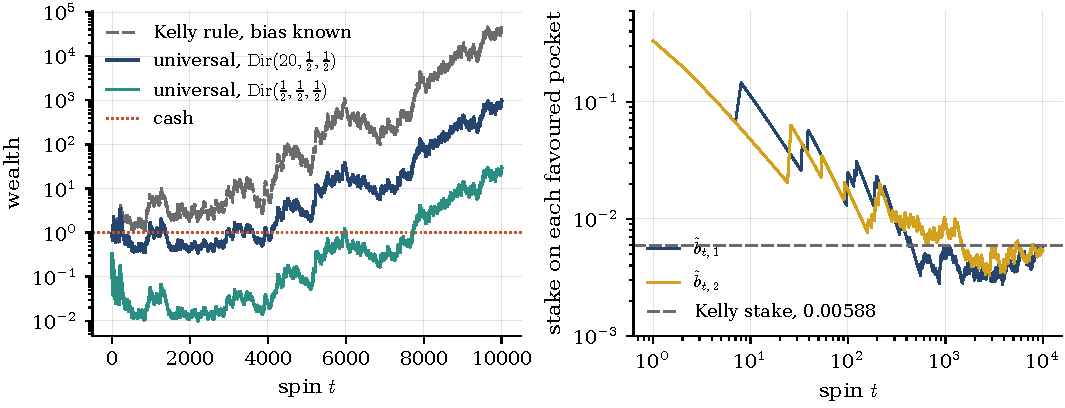
\includegraphics[width=\textwidth]{up_fig_roulette}
\caption{\small Left: wealth on the biased wheel for the Kelly rule with the bias known, for two
universal portfolios differing only in the prior mass on cash, and for cash. Right: the posterior mean
stake on each favored pocket under $\mathrm{Dir}(\frac12,\frac12,\frac12)$, falling from an opening
$1/3$ to the Kelly stake $0.00588$.}
\label{up:fig:roulette}
\end{figure}

\paragraph{Kurtz's rule and the exchange rate between a level and a prior.} The direct Bayesian
suggestion is to put $\mathrm{Dir}(c,\dots,c)$ on the $38$ pocket probabilities, form the posterior
mean $\bar p_j=(n_j+c)/(n+38c)$, and stake $b^\star(\bar p)$ by water filling. Because the growth rate
$\sum_jp_j\log(b_0+o_jb_j)$ is linear in $p$, the posterior expected growth is exactly the growth at
$\bar p$, so this plug in is the Bayes rule for the growth criterion and is available in closed form
in any dimension. It is also conservative: the stake $(p_j-b_0^\star/o_j)_+$ is convex in $p_j$, so
averaging the rule over the posterior stakes more than the rule at the posterior mean, which stakes
exactly zero until a pocket clears the break even frequency.

\begin{proposition}[Bayesian entry threshold]\label{up:prop:threshold}
At gross odds $36$, $\bar p_j>1/36$ if and only if $n_j>n/36+c/18$.
\end{proposition}

\begin{proof}
$36(n_j+c)>n+38c$ rearranges to $36n_j>n+2c$.
\end{proof}

The Bayes threshold and Ethier's test have identical centering and differ only in the margin: the
prior buys a constant $c/18$, the test a margin growing like $\sqrt n$. Matching them at horizon $n$
gives $c=18a\sqrt n=8.82\sqrt n$, so reproducing a five percent test over $10\,000$ spins needs $c\approx882$, a
prior worth about $33\,500$ pseudo spins. That is the exchange rate between a significance level and a
prior, and it says something uncomfortable about the $\mathrm{Dir}(\frac12)$ default, which buys a
margin of $1/36$ of a spin. Table~\ref{up:tab:kurtz} shows the cost: with $c=\frac12$ the rule chases
noise across twenty pockets and ends at $e^{-65.8}$ of its capital on the very path where the
universal portfolio made money; $c=200$ ends at $\log S_T=3.24$; and at $c=882$ the rule identifies
exactly the two favored pockets but stakes too little, too late, and earns nothing. Multiplicity does
not disappear when one becomes a Bayesian. It reappears as prior concentration, and the right answer
is not a larger scalar $c$ but a sparse prior that expects most pockets to be fair, the global local
machinery of Section~\ref{ch:hsmdp}.

\begin{table}[t]
\centering\small
\begin{tabular}{rrrrrr}
\toprule
$c$ & margin $c/18$ & active, $n=1000$ & active, $n=10^4$ & stake, $n=10^4$ & $\log S_T$\\
\midrule
$0.5$ & $0.03$ & $20$ & $9$ & $0.0197$ & $-65.85$\\
$10$ & $0.56$ & $16$ & $9$ & $0.0184$ & $-13.57$\\
$50$ & $2.78$ & $10$ & $8$ & $0.0139$ & $1.91$\\
$200$ & $11.1$ & $0$ & $4$ & $0.0058$ & $3.24$\\
$882$ & $49.0$ & $0$ & $2$ & $0.0003$ & $0.00$\\
$2000$ & $111$ & $0$ & $0$ & $0$ & $0.00$\\
\bottomrule
\end{tabular}
\caption{\small Kurtz's rule on the biased wheel for symmetric Dirichlet priors of increasing
concentration. The true Kelly stake is $0.0118$ in total. The row $c=882$ reproduces Ethier's five
percent test at this horizon.}
\label{up:tab:kurtz}
\end{table}

\subsection{Fractional Kelly three ways}
Three different operations are all called fractional Kelly, and the Bayesian reading separates them.
Tempering the posterior to $S_t(b)^\eta\Pi(db)$ with $\eta<1$ slows learning and pulls the mean toward
the prior; it breaks Theorem~\ref{up:thm:evidence}, which holds only at $\eta=1$. Risk aversion with
power utility $\gamma\ne1$ makes $b\mapsto(b^\top x)^{1-\gamma}$ nonlinear, so the mixture of wealths
is no longer the wealth of a mixture; what survives is the Merton (1969) scaling $\omega^\star=\mu/(\gamma\sigma^2)$.
On the biased wheel the exact $\gamma=2$ rule stakes $0.00282$ per pocket, $0.479$ of Kelly rather than
one half, keeps $74.3$ percent of the growth rate, and halves the standard deviation of log wealth
from $0.0484$ to $0.0242$ per spin. In the continuous limit with fraction $\alpha$ of Kelly, Thorp records
that the probability of ever falling to half the starting wealth is $(\frac12)^{2/\alpha-1}$ and the growth
rate relative to the maximum is $\alpha(2-\alpha)$; full Kelly halves the stake at some point with probability
one half, half Kelly with probability one eighth while keeping three quarters of the growth. The third
route needs no risk aversion: by \eqref{up:eq:shrink} the posterior mean already plays a data dependent
fraction of Kelly. On the wheel the implied fraction $(\hat b_{t,1}+\hat b_{t,2})/(b_1^\star+b_2^\star)$
under $\mathrm{Dir}(\frac12,\frac12,\frac12)$ is $56.6$ at the first spin, $3.64$ at $t=100$, $0.75$ at
$t=3000$, $0.73$ at $t=5000$ and $0.94$ at $t=10\,000$; under $\mathrm{Dir}(20,\frac12,\frac12)$ it
opens at $4.05$ and follows nearly the same path thereafter. The card counter's half or third of Kelly
(Section~\ref{sec:thorp}) and the posterior mean arrive at similar numbers for entirely different
reasons, and only the second carries a guarantee.

\subsection{The continuous limit: what learning is worth}
Browne and Whitt (1996) settle when plugging a posterior mean into the optimal rule is exactly right.
For a drift $Z$ observed through $dX_t=Z\,dt+\sigma\,dW_t$, any prior, and a bond paying $r$, the
log optimal control is the certainty equivalent $f_t^\star=(\E[Z\mid\mathcal F_t]-r)/\sigma^2$, the
Merton rule at the posterior mean drift, because the log value function is additively separable in
wealth, the same fact that makes Theorem~\ref{up:thm:evidence} telescope. Under a conjugate
$Z\sim\mathcal N(\mu_0,\tau^2)$ the expected log wealths $F_T$, $F^B_T$ and $F^P_T$ from playing the prior mean, from learning, and from being told the drift
satisfy
\begin{equation}\label{up:eq:learn}
F^B_T-F_T=\frac{\tau^2T}{2\sigma^2}+\frac12\log\frac{\sigma^2}{\sigma^2+\tau^2T},\qquad
F^P_T-F^B_T=\frac12\log\Bigl(1+\frac{\tau^2T}{\sigma^2}\Bigr).
\end{equation}
Learning is worth a quantity growing linearly in the horizon and costs a quantity growing
logarithmically, and the cost is $\frac12\log T+O(1)$, the case $d=2$ of Theorem~\ref{up:thm:regret}.
Universal portfolios, stochastic complexity and continuous time Bayesian control arrive at the same
$\frac{d-1}2\log T$ for the same reason: $d-1$ parameters learned at rate $t^{-1/2}$ cost $O(1/t)$ per
period, and $\sum_{t\le T}1/t\sim\log T$ (Figure~\ref{up:fig:learning}). For power utility certainty
equivalence fails already at a two step horizon, and Jacquier and Polson show that the optimal
exchangeable Bernoulli bettor then stakes a positive amount on a bet whose posterior odds are
unfavorable, buying information; under log utility the separability that gives
Theorem~\ref{up:thm:evidence} also removes that incentive to explore.

\begin{figure}[H]
\centering
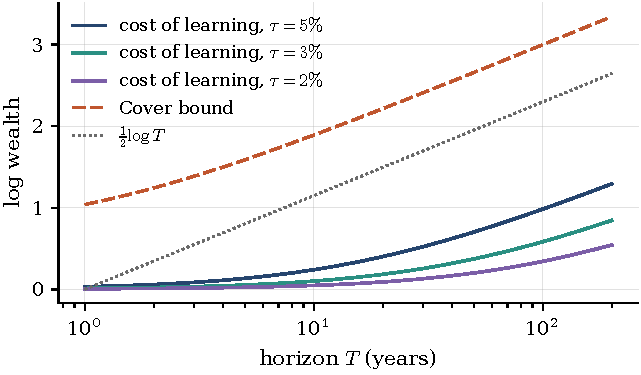
\includegraphics[width=0.62\textwidth]{up_fig_learning}
\caption{\small The cost of learning \eqref{up:eq:learn} for three prior standard deviations, against the
Cover and Ordentlich bound and the asymptotic rate, $\sigma=0.2016$. All curves share a slope on the
log horizon axis; what the prior buys is the intercept.}
\label{up:fig:learning}
\end{figure}

\subsection{Finite samples: the prior is the only instrument}
Theorem~\ref{up:thm:regret} splits regret into $\frac{d-1}2\log\frac T{2\pi}+\frac12\log\det\Info(b^\star)$, which no prior can touch, and
$-\log\pi(b^\star)$, which is entirely the investor's to choose. The second term need not
be small: on the biased wheel, moving prior mass to cash lowers it by $3.5$, against $\frac{d-1}2\log\frac T{2\pi}=7.37$ at $d=3$ and $T=10\,000$. So the practical content of the Bayesian reading is short: the prior is the
instrument, it acts as shrinkage of the empirical log optimal portfolio, and with one risky asset and
a conjugate prior $\mu\sim\mathcal N(\mu_0,\tau^2)$ on the excess drift it gives the rule
\begin{equation}\label{up:eq:bayeskelly}
\omega_T=\frac{\mu_T}{\sigma^2+v_T},\qquad
\mu_T=\frac{\hat\mu\,T/\sigma^2+\mu_0/\tau^2}{T/\sigma^2+1/\tau^2},\qquad
v_T=\Bigl(\frac T{\sigma^2}+\frac1{\tau^2}\Bigr)^{-1},
\end{equation}
in which parameter uncertainty shrinks the numerator and inflates the denominator, as in
Remark~\ref{prop:fractional}. The rule is for a position held one period; held for $h$ periods the denominator is $\sigma^2+h\,v_T$, which tends to $\sigma^2$ as $h\to0$, so the certainty equivalence of Browne and Whitt is its continuous time limit.

\paragraph{One hundred and fifty two years of the SP500.} Shiller's monthly series with dividends,
with the long rate as the riskless proxy, gives $1829$ monthly excess returns from 1871 to 2023, an
annual mean excess return of $5.40$ percent at volatility $14.08$ percent, and a full sample Kelly
allocation of $2.72$ with standard error $0.58$. Walk the rules forward, using only data available at
each date, holding each month's position for a month, capping leverage at two, after a ten year burn
in. Table~\ref{up:tab:shiller} and Figure~\ref{up:fig:shiller} report the result under an
$\mathcal N(5\%,2\%^2)$ prior on the annual excess drift. In 1900 the plug in allocation is $2.59$
with standard error $1.72$, an interval from no position to six times levered; after about 1950 the
two rules coincide because the data dominate. The whole difference in terminal wealth, a factor of
$1.45$, is made in the early period. The prior buys nothing asymptotically and everything at the
start.

\begin{table}[t]
\centering\small
\begin{tabular}{lrrr}
\toprule
Rule & terminal wealth & $\log S_T$ & annual growth\\
\midrule
Cash at the long rate & $488$ & $6.19$ & $4.35\%$\\
The index, fully invested & $245\,800$ & $12.41$ & $8.72\%$\\
Plug in Kelly, capped at two & $3\,653\,900$ & $15.11$ & $10.61\%$\\
Bayes rule, capped at two & $5\,312\,500$ & $15.49$ & $10.87\%$\\
Kelly with hindsight, capped at two & $6\,227\,300$ & $15.64$ & $10.98\%$\\
\bottomrule
\end{tabular}
\caption{\small Walk forward on Shiller's SP500 series, 1881 to 2023, monthly rebalancing, one dollar
in 1881. The Bayes rule beats the plug in rule by $0.37$ in log wealth and gives up $0.16$ to an
allocation that could only be computed at the end (differences of the unrounded logarithms).}
\label{up:tab:shiller}
\end{table}

\begin{figure}[H]
\centering
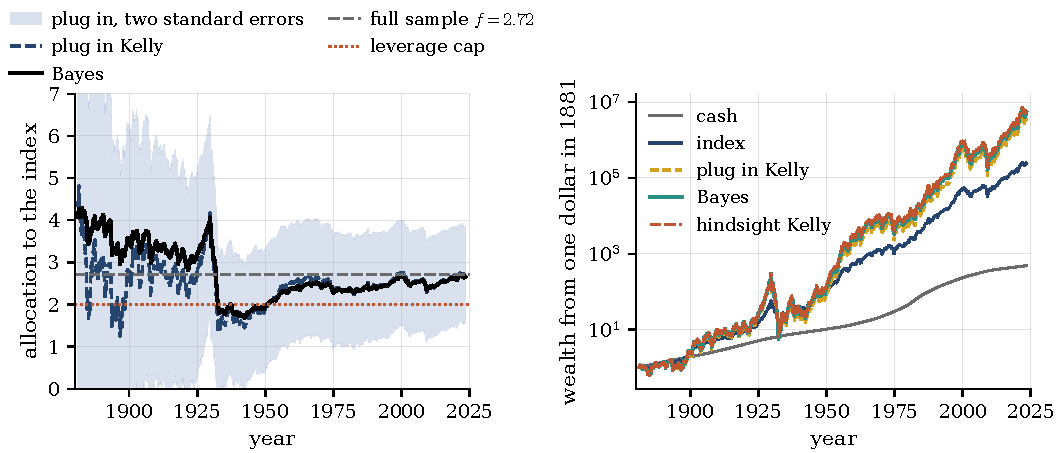
\includegraphics[width=\textwidth]{up_fig_shiller}
\caption{\small Left: the allocation implied by the data available at each date, the plug in rule with
its two standard error band, the Bayes rule under an $\mathcal N(5\%,2\%^2)$ prior, the full sample
value and the leverage cap. Right: wealth from one dollar in 1881.}
\label{up:fig:shiller}
\end{figure}

\paragraph{Thorp's Berkshire Hathaway calculation.} Berkshire traded at $20$ in 1964 and $70\,000$
in 1998. Thorp (2006, Example 7.3) does not use the realized instantaneous drift of $0.24$; arguing for
regression to the mean, the drag of size and management risk, he takes $m=0.20$, $s=0.15$, $r=0.06$,
giving $f^\star=(m-r)/s^2=6.22$, then caps leverage at $2$ because prices jump. The input is fragile:
across the values in his own paper the Kelly leverage moves between $2.43$ and $8.00$ without anyone
making an error, and with thirty four years of data at volatility $0.2016$ the standard error of
$f^\star$ is about $0.85$. Write the judgment as a prior instead. With the realized excess drift $0.18$
and standard error $0.035$, the rule \eqref{up:eq:bayeskelly} gives Table~\ref{up:tab:brk}. A prior
that puts the equity premium at five percent and treats a sustained excess of about nine percent as a
two standard deviation event returns $f=2.02$, the number Thorp reached by argument, and the same
prior at $\gamma=2$ returns almost exactly the unlevered position. Both of Thorp's adjustments, the shaved drift and the leverage cap,
are made here by the numerator of \eqref{up:eq:bayeskelly}, since $v_T=3.0\times10^{-4}$ adds under one percent to $\sigma^2=0.041$; stating them as a prior makes the
judgment explicit and revisable and removes the temptation to apply it twice
(Figures~\ref{up:fig:thorp} and~\ref{up:fig:growth}). The asymmetry in the left panel of
Figure~\ref{up:fig:growth} is the case for shrinkage: growth is a concave parabola in the allocation, so underbetting
costs at most the edge and overbetting without limit.

\begin{table}[t]
\centering\small
\begin{tabular}{lrrrr}
\toprule
Prior on the excess drift & posterior mean & posterior sd & $f$ & $f$ at $\gamma=2$\\
\midrule
None, plug in $\hat\mu/\sigma^2$ & $0.180$ & $0.035$ & $4.43$ & $2.21$\\
$\mathcal N(10\%,5\%^2)$ & $0.154$ & $0.028$ & $3.72$ & $1.86$\\
$\mathcal N(5\%,5\%^2)$ & $0.138$ & $0.028$ & $3.33$ & $1.66$\\
$\mathcal N(5\%,3\%^2)$ & $0.106$ & $0.023$ & $2.57$ & $1.29$\\
$\mathcal N(5\%,2\%^2)$ & $0.083$ & $0.017$ & $2.02$ & $1.01$\\
\bottomrule
\end{tabular}
\caption{\small The Bayesian version of Thorp's judgment for Berkshire, $\sigma=0.2016$, thirty four
years. The first row is the plug in rule; the others use \eqref{up:eq:bayeskelly}. The last row
reproduces Thorp's practical leverage of two.}
\label{up:tab:brk}
\end{table}

\begin{figure}[H]
\centering
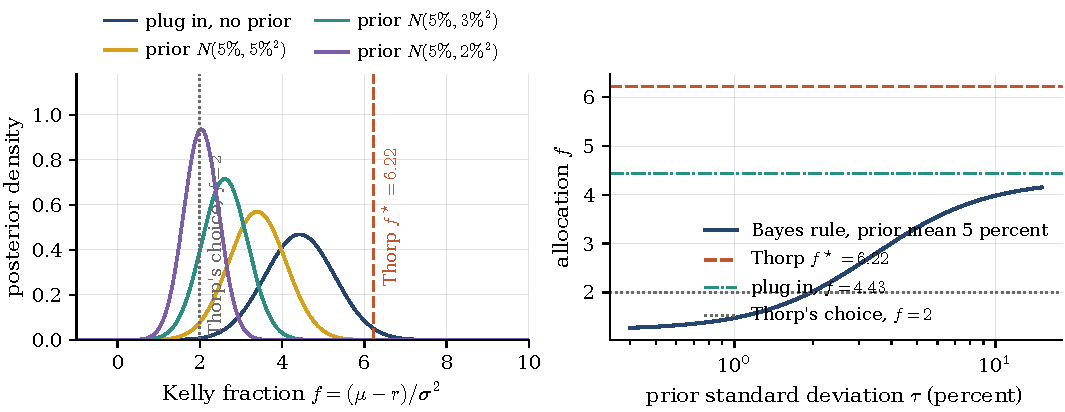
\includegraphics[width=\textwidth]{up_fig_thorp}
\caption{\small Left: posterior of the Kelly fraction for Berkshire under four priors, against Thorp's
$f^\star=6.22$ and his choice of $2$. Right: the Bayes allocation as the prior standard deviation
grows, from the prior mean rule to the plug in rule; about two percent reproduces Thorp.}
\label{up:fig:thorp}
\end{figure}

\begin{figure}[H]
\centering
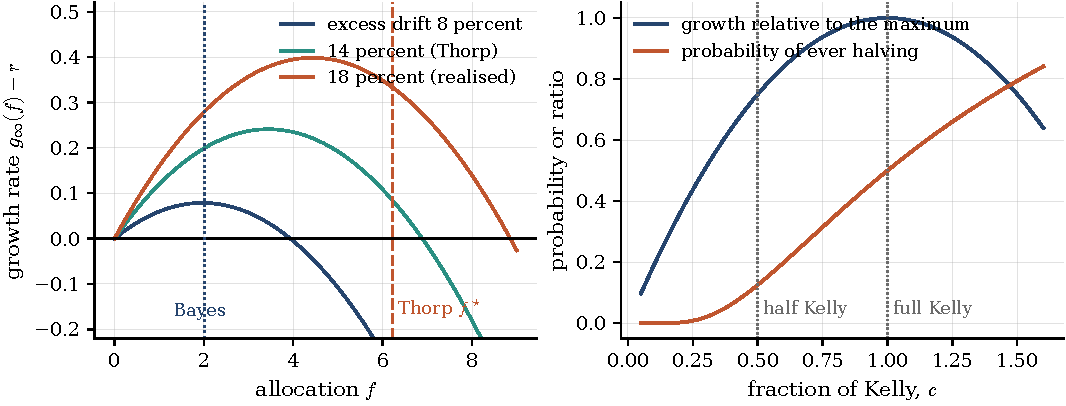
\includegraphics[width=\textwidth]{up_fig_growth}
\caption{\small Left: growth rate against allocation for three true excess drifts, with Thorp's
$f^\star$ and the Bayes allocation marked. Right: growth relative to the maximum and the probability of
ever halving, against the fraction of Kelly played.}
\label{up:fig:growth}
\end{figure}

\paragraph{The whole index.} Now let the assets be the $470$ constituents with a complete five year
daily history, $T=1258$. The best single stock in hindsight multiplied by $18.5$ and the median stock
by $1.71$; the best constant rebalanced portfolio, found by Cover's fixed point iteration, ends at
$2.107$ and the daily rebalanced equal weight portfolio at $1.915$ (Figure~\ref{up:fig:sp470}). The
hindsight optimum is not concentrated: every name carries positive weight and the largest is
$0.0047$, against $0.0021$ for equal weights. The entire prize for knowing the optimum in advance is
$0.095$ in log wealth, while the bound \eqref{up:eq:co} is $\log2+\frac{469}2\log(T+1)=1674.6$, about
seventeen thousand times the quantity it guarantees. Shrinking the monthly refreshed empirical log
optimal weights toward equal weights moves log wealth monotonically from $0.682$ to $0.650$: here the
surface is so flat that there is little for estimation error to damage, and shrinkage is cheap
insurance rather than a source of gain. The plug in mean variance solution on the same data is a
different animal: the sample covariance $\hat\Sigma$ has condition number $6.2\times10^3$ and $\hat\Sigma^{-1}\hat\mu$,
with $\hat\mu$ the vector of mean daily net returns, runs a
gross leverage of $1563$ for a net position of $4.06$. The simplex and the concavity of the logarithm
keep the log optimal problem inside the region the data can see. Two caveats belong with these
numbers: the names are survivors, which biases every row upward, and daily rebalancing across hundreds
of names incurs transaction costs, the setting of Blum and Kalai.

\begin{figure}[H]
\centering
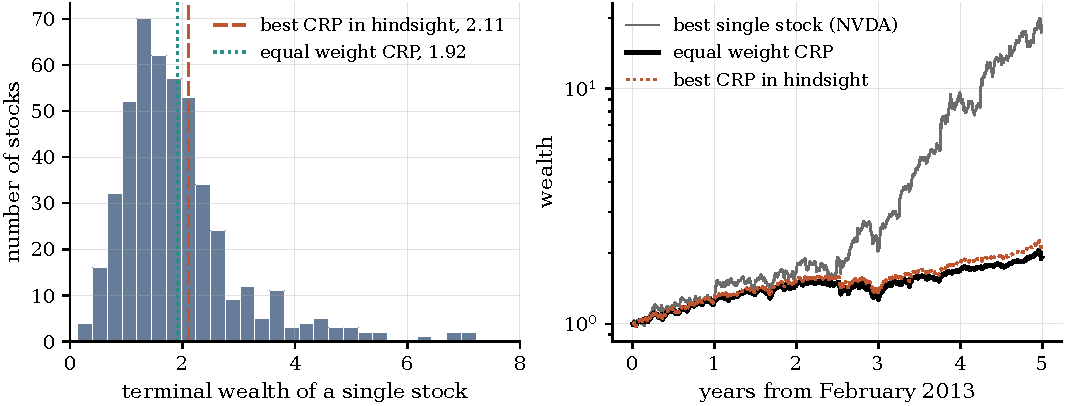
\includegraphics[width=\textwidth]{up_fig_sp470}
\caption{\small Left: terminal wealth across the $470$ constituents, with the hindsight optimal and
equal weight portfolios marked. Right: wealth paths. The hindsight optimum and equal weights are
nearly the same object.}
\label{up:fig:sp470}
\end{figure}

\subsection{What the example teaches}
Read as a Bayes rule, Cover's construction identifies the prior that matters and says why (Jeffreys,
by the equalizer property), replaces a combinatorial regret calculation by a Laplace expansion, and
makes the finite sample behavior, shrinkage toward the prior mean, explicit and tunable. Its regret
is a log Bayes factor and the logarithmic score is the only proper local score whose accumulated value
is the logarithm of a bank balance, which is Kelly's observation and the reason the reading is exact
rather than suggestive. The example also marks a boundary: at realistic dimensions the uniform
guarantee is uninformative, and all the practical work is done by the prior, by screening, and by
sparsity, as in the testing and shrinkage sections.

\subsection*{Problems}
\begin{enumerate}[leftmargin=2em]
\item Prove Proposition~\ref{up:prop:grid} and show that for any finite mixture prior the grid
recursion and the integral form \eqref{up:eq:post} produce identical wealth paths.
\item In the horse race market with $\mathrm{Dir}(\alpha,\dots,\alpha)$, compute $m_T$ in closed form and
show that $\alpha=\frac12$ makes the leading data dependent terms of $R_T$ cancel.
\item For the Parrondo market, derive $\Info=2p(1-p)(2f)^2$ and the growth rates of a single asset and of
the equal weight portfolio. For which $(p,f)$ does volatility pumping turn two losing assets into a
winner?
\item Prove Proposition~\ref{up:prop:threshold} for general gross odds $o$ and $k$ pockets, and find the
concentration $c$ that matches a level $\alpha$ screening test at horizon $n$.
\item Verify \eqref{up:eq:learn} from the Gaussian posterior for the drift and show that
$F^P_T-F^B_T=\frac12\log T+O(1)$.
\item Using \eqref{up:eq:bayeskelly}, find the prior standard deviation $\tau$ that reproduces Thorp's
leverage of two for Berkshire when $\mu_0=5\%$, and show how that $\tau$ changes if the record were
twice as long.
\end{enumerate}

\src{Polson, ``A Bayesian Interpretation of Cover's Universal Portfolio'' (submitted to
\emph{Entropy}, 2026); Cover (1991); Cover and Ordentlich (1996); Ordentlich and Cover (1998); Clarke
and Barron (1990, 1994); Rissanen (1996); Shtarkov (1987); Krichevsky and Trofimov (1981); Bissiri,
Holmes, and Walker (2016); Parrondo, Harmer, and Abbott (2000); Luenberger (1998); Ethier (1982, 2010);
Klotz (2000); Browne and Whitt (1996); Thorp (2006); Jacquier and Polson (2013); Blum and Kalai (1999).
All tables and figures in this section were recomputed for the book from the public Shiller and SP500
datasets and the simulation code in the book's code archive.}

%====================================================================================================
%====================================================================================================

\section{Nonlinear State-Space Models and Bayesian Filtering}\label{ch:filter}

\noindent\textbf{Thesis.} A state-space model\index{state-space model} is a hidden Markov chain observed
through noise, and Bayesian filtering is the sequential posterior over the hidden
state. When the state dynamics or the observation map are nonlinear or the errors
non-Gaussian, the filtering recursion has no closed form, and the same two tools that
run through this book, data augmentation for the batch problem and sequential Monte
Carlo for the online problem, deliver asymptotically exact inference where the Kalman filter\index{Kalman filter} (Kalman, 1960) cannot.
This section states the filtering recursion, the Monte Carlo solution to nonnormal
and nonlinear smoothing, and the connection to the predictive spine.

\subsection{The filtering recursion}\label{fl:sec:recursion}

A state-space model pairs a state equation $x_t\sim p(x_t\mid x_{t-1},\theta)$ with an
observation equation $y_t\sim p(y_t\mid x_t,\theta)$. Filtering seeks
$p(x_t\mid y_{1:t})$, computed by alternating a prediction step,
$p(x_t\mid y_{1:t-1})=\int p(x_t\mid x_{t-1})p(x_{t-1}\mid y_{1:t-1})\,dx_{t-1}$, and an
update step, $p(x_t\mid y_{1:t})\propto p(y_t\mid x_t)p(x_t\mid y_{1:t-1})$. When both
equations are linear and Gaussian these integrals are the Kalman recursion; otherwise
they are intractable and must be approximated. The one-step predictive
$p(y_t\mid y_{1:t-1})=\int p(y_t\mid x_t)p(x_t\mid y_{1:t-1})\,dx_t$ is the object that
scores the model sequentially, and its running product is the prequential code of
Section~\ref{ch:evalues}: filtering is the state-space instance of the predictive,
one-step-ahead view of Bayesian learning.

\subsection{Monte Carlo smoothing for nonnormal, nonlinear models}\label{fl:sec:smooth}

The batch problem, recover the whole state path $x_{1:T}$ given all the data, is
solved by treating the states as missing data and sampling them. For a nonnormal,
nonlinear model the joint complete conditional of the states is not standard, but a
single-state or block update, drawing $x_t$ given its neighbors and the datum $y_t$,
has a tractable conditional that a Metropolis or accept--reject step handles, and
sweeping through the path realizes a Gibbs sampler over the states with the
parameters updated conditionally. This was the route by which nonnormal and nonlinear
state-space models first became exactly estimable rather than approximated by the
extended Kalman filter, and it is the direct ancestor of the stochastic-volatility
sampler, where the state is log-variance and the observation
error is $\log\chi^2$. The forward-filter backward-sample recursion draws the whole
Gaussian state path in one block whenever a mixture-of-normals representation restores
conditional linearity.

\subsection{Sequential filtering and the predictive}\label{fl:sec:seq}

For the online problem the particle methods for stochastic-volatility models carry the
filtering distribution forward one observation at a time, reweighting by the
predictive likelihood and resampling to fight degeneracy, with parameter learning
handled by the sufficient-statistic recursion of particle learning\index{particle learning}. The filtered
predictive density is again the deliverable, and the sequence of one-step predictives
is again a martingale-posterior factorization, so nonlinear filtering, stochastic
volatility, and the martingale-posterior view of Section~\ref{ch:evalues} are three
readings of one recursion. The Bayesian filter is where the predictive thesis of the
book becomes an algorithm that runs in real time.


\begin{algorithm}[Forward-Filter Backward-Sample]\label{fl:alg:ffbs}
\begin{algorithmic}[1]
\State \textbf{Forward:} for $t=1,\dots,T$ compute the filtered $p(x_t\mid y_{1:t})$ by
predict-then-update, storing its moments.
\State Draw the terminal state $x_T\sim p(x_T\mid y_{1:T})$.
\For{$t=T-1,\dots,1$}
 \State Draw $x_t\sim p(x_t\mid x_{t+1},y_{1:t})\propto p(x_{t+1}\mid x_t)\,p(x_t\mid y_{1:t})$.
\EndFor
\State Return the sampled path $x_{1:T}$.
\end{algorithmic}
\end{algorithm}

\noindent When a mixture-of-normals representation makes the system conditionally
linear-Gaussian, as for a stochastic-volatility model, each
draw on line 4 is Gaussian, and the whole state path is sampled in one $O(T)$ backward
sweep.





\subsection*{Worked example: the steady-state Kalman filter}
This example solves the filtering recursion for its fixed point in closed form, exposing how quickly the filter forgets.

The Kalman filter for $x_t=x_{t-1}+w_t$, $y_t=x_t+v_t$ with unit noises updates the posterior variance by $P_t=\big((P_{t-1}+1)^{-1}+1\big)^{-1}$, whose fixed point solves $P=1/((P+1)^{-1}+1)$, i.e.\ $P=(\sqrt5-1)/2$, the golden ratio minus one. The steady-state Kalman gain is $K=(P+1)/(P+2)=1/(P+1)$, showing the filter forgets old data at a geometric rate set by the signal-to-noise ratio.

The steady-state variance is a fixed point of the Riccati recursion, and its value is set entirely by the signal-to-noise ratio of the model. The resulting constant gain discounts old observations geometrically, which is why a linear-Gaussian state-space model has a finite effective memory rather than an unbounded one.

\paragraph{Summary.}
A state-space model is a hidden Markov chain observed through noise; filtering alternates a prediction and an update step, and the one-step predictive is the prequential code. Nonnormal, nonlinear models are fit by sampling the state path (data augmentation) or by particle methods online.

\subsection*{Problems}
\begin{enumerate}[leftmargin=2.2em,itemsep=2pt]
\item Write the predict and update steps of the filtering recursion and specialize to the Kalman filter.
\item Show the one-step predictive $p(y_t\mid y_{1:t-1})$ and its running product form the prequential code.
\item Describe forward-filter backward-sample and the mixture-of-normals trick that restores conditional linearity.
\item Derive the extended and unscented approximations and state when they fail.
\item Relate the filter to the martingale posterior of Section~\ref{ch:evalues}.
\end{enumerate}

\src{A Monte Carlo Approach to Nonnormal and Nonlinear State-Space Modeling (Carlin,
Polson and Stoffer, 1992); Particle Learning and Smoothing (Carvalho, Johannes, Lopes
and Polson, 2010); MCMC Methods for Financial Econometrics (Johannes and Polson,
2010); the predictive/martingale-posterior view of Section~\ref{ch:evalues}.}

%====================================================================================================

\section{Hamiltonian and Langevin Monte Carlo}\label{ch:hmc}

\noindent\textbf{Thesis.} Gradient information turns random-walk sampling into
directed exploration. Hamiltonian Monte Carlo\index{Hamiltonian Monte Carlo} simulates a physical trajectory that
carries the state far across the posterior in a single move, and Langevin dynamics is
its overdamped limit, the same diffusion whose discretization is the noisy gradient
descent of Section~\ref{ch:deep}. This section states both, their shared geometry, and
why they are the default samplers for the smooth, high-dimensional posteriors of
modern Bayesian models.

\subsection{Hamiltonian dynamics as a proposal}\label{hm:sec:ham}

Augment the parameter $\theta$ with a momentum $r$ and define the Hamiltonian
$H(\theta,r)=-\log p(\theta\mid y)+\tfrac12 r^\top M^{-1}r$, the negative log-posterior
as potential energy plus a Gaussian kinetic energy. Hamilton's equations conserve $H$
and preserve volume, so simulating them for a fixed time and accepting by a Metropolis
step that corrects the discretization error gives a proposal that moves along level
sets of the Hamiltonian rather than diffusing across them. The leapfrog integrator
alternates half-steps in momentum and full steps in position, keeping the map
volume-preserving and reversible so the acceptance ratio depends only on the small
energy error. A single trajectory of many leapfrog steps travels a distance that a
random walk would need quadratically many steps to cover, which is why Hamiltonian
Monte Carlo scales to hundreds of dimensions where Metropolis stalls. The no-U-turn
extension removes the need to tune the trajectory length by running until the path
begins to double back.

\subsection{Langevin dynamics and the diffusion limit}\label{hm:sec:lange}

Taking the momentum to be resampled every step and the step size to zero gives the
overdamped Langevin diffusion $d\theta=\tfrac12\nabla\log p(\theta\mid y)\,dt+dW$,
whose stationary distribution is the posterior. Its Euler discretization is the
Metropolis-adjusted Langevin algorithm, a gradient step plus Gaussian noise plus a
Metropolis correction, and dropping the correction gives the unadjusted Langevin
algorithm; a minibatch gradient with decreasing steps turns it into the stochastic
gradient Langevin dynamics that trains Bayesian neural networks. This is the exact
diffusion of Section~\ref{ch:deep}: stochastic gradient descent with the right noise
is Langevin sampling, and the boundary between optimization and inference is again the
noise scale. The posterior geometry enters through the gradient, so both Hamiltonian
and Langevin methods degrade when the posterior is poorly conditioned or multimodal,
and both are preconditioned by a mass matrix or a Riemannian metric that rescales the
dynamics to the local curvature.

\subsection{Geometry and the Fisher metric}\label{hm:sec:geom}

The natural preconditioner is the Fisher information, which makes the sampler invariant
to reparameterization and turns the kinetic part of the dynamics into geodesic flow on the statistical
manifold. Riemannian Hamiltonian Monte Carlo uses the Fisher metric as the mass matrix,
so the trajectories follow the intrinsic geometry of the model rather than the
arbitrary coordinates it is written in, and the moderate-deviation, information-metric
picture of Section~\ref{ch:evalues} reappears as the geometry the sampler exploits.
The unifying statement is that all three, Hamiltonian, Langevin, and their
Riemannian forms, are gradient-driven flows whose stationary law is the posterior and
whose efficiency is set by how well their metric matches the posterior's curvature,
the same curvature the Laplace approximation and the BIC penalty measure.


\begin{algorithm}[Leapfrog Hamiltonian Monte Carlo]\label{hm:alg:leap}
\begin{algorithmic}[1]
\State Given $\theta$, draw momentum $r\sim\N(0,M)$; set $(\theta_0,r_0)=(\theta,r)$.
\For{$\ell=1,\dots,L$}
 \State $r\leftarrow r+\tfrac{\epsilon}{2}\nabla\log p(\theta\mid y)$ \Comment{half momentum step}
 \State $\theta\leftarrow \theta+\epsilon\,M^{-1}r$ \Comment{full position step}
 \State $r\leftarrow r+\tfrac{\epsilon}{2}\nabla\log p(\theta\mid y)$ \Comment{half momentum step}
\EndFor
\State Accept $(\theta,r)$ with prob.\ $\min\{1,\exp(H(\theta_0,r_0)-H(\theta,r))\}$.
\end{algorithmic}
\end{algorithm}

\noindent The split half-steps on lines 3--5 make the leapfrog map volume-preserving
and reversible, so the only error is in the conserved energy $H$, and that error is
corrected exactly by the acceptance step on line 7.


\subsection{A guide to the samplers}\label{hm:sec:guide}

The book's samplers form a short hierarchy, ordered by how much structure they exploit.

\begin{table}[h]\centering\small
\begin{tabular}{@{}llll@{}}
\toprule
Sampler & Uses & Cost/step & Best for \\
\midrule
Random-walk Metropolis & density & cheap & low dimension \\
Gibbs / data augmentation & conditionals & cheap & conditionally conjugate \\
Slice sampling & density & cheap & 1-d conditionals \\
MALA / Langevin & gradient & moderate & smooth, high-d \\
Hamiltonian MC & gradient & moderate & smooth, high-d, correlated \\
Riemannian HMC & gradient, metric & high & ill-conditioned \\
Particle / SMC & simulator & high & state-space, online \\
Particle MCMC & simulator & very high & intractable-likelihood \\
\bottomrule
\end{tabular}
\caption{Monte Carlo samplers ordered by the structure they exploit. More structure
buys better mixing at higher per-step cost; the right choice matches the posterior's
geometry and the model's tractability.}\label{hm:tab:samplers}
\end{table}

\noindent The rule the book applies throughout is to exploit as much structure as the
model exposes: conditional conjugacy for a Gibbs sweep, gradients for Hamiltonian
dynamics, a simulator for particle methods, and to accept the higher per-step cost
only when the geometry demands it.





\subsection*{Worked example: one Hamiltonian trajectory}
This example shows why Hamiltonian Monte Carlo can cross a distribution in one trajectory rather than diffusing across it.

For a standard Gaussian target, one leapfrog step of size $\epsilon$ with unit mass rotates $(\theta,r)$ by an angle $\approx\epsilon$ in phase space, so a trajectory of $L$ steps traverses angle $\epsilon L$; choosing $\epsilon L\approx\pi/2$ sends $(\theta,r)$ to $(r,-\theta)$, so a single proposal moves the position to the initial momentum, an independent draw from the target. A random walk would need $\sim(\epsilon L)^2/\epsilon^2=L^2$ steps to cover the same distance, the quadratic speed-up of HMC.

On a Gaussian target the leapfrog integrator rotates position and momentum through phase space, so a trajectory of the right length carries the sampler from one side of the distribution to the other in a single proposal. This ballistic motion, rather than the random walk of a naive sampler, is what gives Hamiltonian methods their efficiency in high dimension.

\paragraph{Summary.}
Hamiltonian Monte Carlo augments with momentum and simulates a volume-preserving, reversible trajectory, moving far per step; Langevin dynamics is its overdamped limit and the SGLD sampler of deep learning. The Fisher metric is the natural preconditioner.

\subsection*{Problems}
\begin{enumerate}[leftmargin=2.2em,itemsep=2pt]
\item Show the leapfrog integrator is volume-preserving and reversible.
\item Derive the Metropolis acceptance for HMC from energy conservation error.
\item Show the overdamped Langevin diffusion has the posterior as its stationary law.
\item Explain why HMC scales better than random-walk Metropolis in high dimension.
\item Describe Riemannian HMC and the role of the Fisher metric.
\end{enumerate}

\src{Hamiltonian Monte Carlo (Duane et al., 1987; Neal, 2011); the no-U-turn sampler (Hoffman and
Gelman, 2014); Riemannian manifold HMC (Girolami and Calderhead, 2011); stochastic gradient
Langevin dynamics (Welling and Teh, 2011); the SGD-as-sampling view of Section~\ref{ch:deep}.}

%====================================================================================================

\section{Particle MCMC, SMC\texorpdfstring{$^2$}{2}, and Exact Approximate Inference}\label{ch:pmcmc}

\noindent\textbf{Thesis.} A remarkable fact makes modern state-space inference
possible: a Markov chain that uses an unbiased Monte Carlo estimate of the likelihood
in place of the true likelihood still targets the exact posterior. Particle Markov
chain Monte Carlo builds that unbiased estimate with a particle filter\index{particle filter}, and SMC$^2$
runs particle filters inside a sequential Monte Carlo sweep over parameters. Together
they extend the asymptotic exactness of the stochastic-volatility samplers to
models whose likelihood cannot be written down. This section states the pseudo-marginal\index{pseudo-marginal method}
principle and the two algorithms that exploit it.

\subsection{The pseudo-marginal principle}\label{pm:sec:pseudo}

Let the parameter posterior given data $y$ be $p(\theta\mid y)\propto p(\theta)L(\theta)$ with a
likelihood $L(\theta)$ that is intractable but admits a nonnegative unbiased
estimator $\hat L(\theta)$, $\E[\hat L(\theta)]=L(\theta)$. Run Metropolis--Hastings
using $\hat L$ in the acceptance ratio, carrying the estimate along with the state.
The chain lives on the enlarged space of $(\theta,\hat L)$, and its stationary
$\theta$-marginal is $p(\theta\mid y)$, because the unbiasedness makes the
auxiliary randomness integrate out. This is the pseudo-marginal principle, and it is
the exact-approximate guarantee: the estimated likelihood introduces no bias, only
variance, and the variance of $\log\hat L$ controls the mixing: too noisy an
estimate stalls the chain, so the number of particles is tuned to hold that variance
near one. The principle is the sampling counterpart of the unbiased-evidence identity
that ran through Section~\ref{ch:evalues}.

\subsection{Particle MCMC}\label{pm:sec:pmcmc}

For a state-space model the particle filter delivers the required estimator:
its normalizing-constant output is an unbiased estimate of the likelihood
$p(y_{1:T}\mid\theta)$. Particle marginal Metropolis--Hastings uses that output in the
acceptance ratio, and the particle Gibbs variant conditions on a reference trajectory
so that a single retained path threads through the resampling, giving a valid Gibbs
update of the state path even at moderate particle counts.

\begin{algorithm}[Particle Marginal Metropolis--Hastings]\label{pm:alg:pmmh}
\begin{algorithmic}[1]
\State Initialize $\theta^{(0)}$; run a particle filter to get $\hat L(\theta^{(0)})$.
\For{$k=1,2,\dots$}
 \State Propose $\theta^\ast\sim q(\cdot\mid\theta^{(k-1)})$.
 \State Run a particle filter at $\theta^\ast$ to get the unbiased $\hat L(\theta^\ast)$.
 \State Accept $\theta^\ast$ with probability
 $\min\!\big\{1,\tfrac{p(\theta^\ast)\hat L(\theta^\ast)\,q(\theta^{(k-1)}\mid\theta^\ast)}
 {p(\theta^{(k-1)})\hat L(\theta^{(k-1)})\,q(\theta^\ast\mid\theta^{(k-1)})}\big\}$.
 \State Otherwise set $\theta^{(k)}=\theta^{(k-1)}$ and keep $\hat L(\theta^{(k-1)})$.
\EndFor
\end{algorithmic}
\end{algorithm}

The retained-estimate step on line~6 is what preserves exactness: reusing the old
estimate rather than recomputing it keeps the chain reversible on the enlarged space.

\subsection{SMC-squared}\label{pm:sec:smc2}

Particle MCMC fixes the data and iterates. The online problem, update the parameter
posterior as each observation arrives, is solved by SMC$^2$, which carries a
population of parameter particles, each equipped with its own particle filter over the
states. As a new observation arrives, each parameter particle's filter is advanced and
its incremental likelihood reweights the parameter particle; when the parameter
weights degenerate, a particle-MCMC move rejuvenates them. The result is a fully
sequential sweep over both states and parameters that targets the exact joint
posterior at every time, consistently as the number of parameter particles grows, and extends particle learning to models where sufficient statistics are unavailable. The cost is
quadratic in the particle budget, the price of nesting one Monte Carlo inside another,
and the payoff is asymptotically exact online Bayesian inference for essentially any state-space
model.


\paragraph{Summary.}
An unbiased likelihood estimate can replace the true likelihood in Metropolis--Hastings without biasing the stationary law (the pseudo-marginal principle). Particle filters supply the estimate; SMC$^2$ nests particle filters inside a parameter sweep for asymptotically exact online inference.

\subsection*{Problems}
\begin{enumerate}[leftmargin=2.2em,itemsep=2pt]
\item Prove that the pseudo-marginal chain has the exact $\theta$-marginal stationary law.
\item Show the particle filter's normalizing-constant estimate is unbiased.
\item Explain why the variance of $\log\hat L$ must be kept near one and how the particle count tunes it.
\item Describe particle Gibbs and the role of the retained reference trajectory.
\item Sketch the SMC$^2$ recursion and its quadratic cost.
\end{enumerate}

\src{The pseudo-marginal principle (Andrieu and Roberts, 2009); particle MCMC (Andrieu,
Doucet and Holenstein, 2010); SMC$^2$ (Chopin, Jacob and Papaspiliopoulos, 2013); the particle
learning and filtering view of Section~\ref{ch:filter}.}

%====================================================================================================

\shorthead{Decisions and Reinforcement Learning}
\chapter{Sequential Decisions and Reinforcement Learning}\label{chap:sequential}

When our actions change the data we see, prediction and decision become inseparable. This chapter
develops the sequential-design, bandit, and reinforcement-learning problems in which the predictive
distribution both guides exploration and is reshaped by it.

Bayesian optimization and Thompson sampling use posterior uncertainty as the engine of exploration;
control-as-inference turns planning into a message-passing computation with a Gibbs-optimal policy; and
approximate Bayesian computation handles the likelihood-free simulators these problems often involve.
The moderate-deviation scale returns here as the threshold behind the regret bounds, closing the loop with the
testing and shrinkage boundaries of the earlier chapters.


\section{Bayesian Optimization and Sequential Design}\label{ch:bo}

\noindent\textbf{Thesis.} To optimize an expensive black-box function (a simulator, a
physical experiment, a hyperparameter surface), the efficient strategy is to model the
function with a Gaussian process and choose each evaluation to maximize an acquisition
function of the posterior, such as the expected improvement or the expected information about the optimum. Bayesian optimization\index{Bayesian optimization} is sequential design driven by the
predictive distribution of Section~\ref{ch:gp}, and it is the exploration-exploitation
problem in its cleanest form.

\subsection{The surrogate and the acquisition}\label{bo:sec:acq}

Model the unknown objective $f$ by a Gaussian-process posterior given the evaluations
so far, so that at every untried input there is a predictive mean and variance. The
next evaluation is chosen by maximizing an acquisition function that trades the mean
against the variance: expected improvement\index{expected improvement} scores each candidate by how much it is
expected to beat the current best $f^\star$ (written for minimization), available in closed form under the Gaussian-process posterior,
\[ \mathrm{EI}(x)=(f^\star-\mu(x))\,\Phi(z)+\sigma(x)\,\phi(z),\qquad z=\frac{f^\star-\mu(x)}{\sigma(x)}, \] integrating over the predictive uncertainty; the
upper confidence bound (UCB) adds a multiple of the predictive standard deviation to the
mean (for maximization), $\alpha_{\mathrm{UCB}}(x)=\mu(x)+\beta^{1/2}\sigma(x)$; the knowledge gradient values a candidate by the expected gain in the best posterior mean after evaluating it; and entropy search values it by how
much its evaluation is expected to sharpen the posterior over the location of the optimum. Each is
a one-step Bayesian decision rule, and each balances exploiting regions known to be
good against exploring regions the posterior leaves uncertain. The acquisition is
cheap to optimize because it is a functional of the surrogate, not of the expensive
objective.

\subsection{Sequential design and information}\label{bo:sec:design}

The same machinery is classical optimal experimental design made sequential. A design
criterion (maximize expected information gain, minimize predictive variance) is
evaluated under the current posterior, the most informative experiment is run, the
posterior is updated, and the loop repeats. Particle learning of the Gaussian-process
surrogate, as in Section~\ref{ch:gp}, carries the posterior forward without refitting,
so the design adapts online. The information-gain criterion is the mutual information
between the next observation and the quantity of interest, the same
entropy bookkeeping the book has used for coding and evidence, now driving where to
look next. Sequential design is thus the active-learning face of the predictive
program: the model does not merely fit the data it is given, it chooses the data that
will teach it most.

\subsection{Exploration, exploitation, and regret}\label{bo:sec:regret}

The quality of a strategy is measured by cumulative regret, the gap between the values
it evaluates and the unknown optimum, summed over the budget. Good acquisition rules
have regret that grows sublinearly, so the average regret vanishes and the strategy
converges to the optimum; the rate depends on the smoothness the kernel assumes,
faster for smoother objectives. The upper-confidence-bound rule makes the
exploration-exploitation trade explicit through its confidence multiplier, and its
regret bound is a moderate-deviation statement about the Gaussian-process posterior of
the kind in Section~\ref{ch:deviations}: the confidence multiplier grows like the
square root of the log of the budget while the interval width itself shrinks, and the strategy explores to that
scale. Optimization, design, and testing again share one moderate-deviation
coordinate system.




\subsection*{Worked example: expected improvement in Bayesian optimization}
This example computes the acquisition function that balances exploiting a good mean against exploring a large variance.

With current best $f^\ast=1$ and a candidate whose GP posterior is $\N(0.8,0.5^2)$, the expected improvement is $\mathrm{EI}=(f^\ast-\mu)\Phi(z)+\sigma\phi(z)$ with $z=(1-0.8)/0.5=0.4$, giving $\mathrm{EI}=0.2\cdot\Phi(0.4)+0.5\cdot\phi(0.4)\approx0.2(0.655)+0.5(0.368)\approx0.315$. A more uncertain candidate with the same mean but $\sigma=1$ scores higher, so EI rewards exploration.

Expected improvement rewards a candidate both for a promising mean and for a wide posterior, so it will probe an uncertain region even when its expected value is unremarkable. The two terms are exploitation and exploration, and the posterior variance, not any external schedule, is what supplies the exploration.

\paragraph{Summary.}
Bayesian optimization models an expensive objective by a Gaussian process and evaluates where an acquisition function is largest; expected improvement and UCB trade the predictive mean against its variance. Sequential design is the active-learning face of the predictive program, with sublinear regret.

\subsection*{Problems}
\begin{enumerate}[leftmargin=2.2em,itemsep=2pt]
\item Derive the closed-form expected improvement under the GP posterior.
\item State the UCB acquisition and explain its confidence multiplier.
\item Show the information-gain criterion is the mutual information between the next evaluation and the optimum.
\item Sketch the GP-UCB sublinear regret bound and its $\sqrt{\log t}$ confidence multiplier (the interval width itself shrinks).
\item Explain how particle learning of the surrogate makes the design online.
\end{enumerate}

\src{Bayesian optimization and expected improvement (Jones, Schonlau and Welch, 1998;
Mo\v{c}kus, 1975); particle learning for sequential design (Gramacy and Polson, 2011);
GP-UCB regret (Srinivas et al., 2012); the predictive GP view of Section~\ref{ch:gp}.}

%====================================================================================================

\section{Thompson Sampling and Bayesian Bandits}\label{ch:thompson}

\noindent\textbf{Thesis.} When actions must be chosen repeatedly under uncertainty and
each choice both earns a reward and reveals information, the optimal tension between
learning and earning is resolved by a strikingly simple rule: act as if a single
sample from the posterior were the truth. Thompson sampling\index{Thompson sampling} is that rule, and it is the
sequential, decision-theoretic program of the book applied to the multi-armed bandit\index{multi-armed bandit},
where the predictive distribution chooses the action.

\subsection{The bandit problem}\label{th:sec:bandit}

A decision maker faces $K$ arms, each with an unknown reward distribution, and at each
round pulls one arm and observes its reward. Pulling the apparent best arm exploits
current knowledge but forgoes learning about the others; pulling an uncertain arm
explores but risks a low reward. The regret is the shortfall against always pulling the
true best arm, and the goal is to make it grow as slowly as possible. The problem is the
purest form of the exploration-exploitation trade, and its solution sets the template
for reinforcement learning\index{reinforcement learning} and sequential experimentation.

\subsection{Thompson sampling}\label{th:sec:ts}

Maintain a posterior over each arm's reward parameter. At each round, draw one sample
from each arm's posterior and pull the arm with the largest sampled value; observe the
reward and update that arm's posterior. The rule needs no explicit exploration
bonus: the exploration is supplied automatically by the posterior spread, since an
uncertain arm sometimes draws a high sample and gets tried, while a well-estimated
inferior arm rarely does. For Bernoulli rewards the posteriors are Beta and the update
is conjugate; for Gaussian rewards they are Gaussian; in each case the algorithm is a
single posterior draw and a single conjugate update per round, and it is trivially
parallelizable and robust to delayed feedback.

\begin{algorithm}[Thompson Sampling for Bernoulli Bandits]\label{th:alg:ts}
\begin{algorithmic}[1]
\State Initialize $(\alpha_k,\beta_k)=(1,1)$ for each arm $k$.
\For{$t=1,2,\dots$}
 \State Draw $\theta_k\sim\mathrm{Beta}(\alpha_k,\beta_k)$ for each arm $k$.
 \State Pull arm $a_t=\arg\max_k\theta_k$ and observe reward $r_t\in\{0,1\}$.
 \State Update $(\alpha_{a_t},\beta_{a_t})\mathrel{+}=(r_t,\,1-r_t)$.
\EndFor
\end{algorithmic}
\end{algorithm}

\subsection{Regret and the predictive}\label{th:sec:regret}

For Bernoulli rewards, Thompson sampling attains the optimal logarithmic regret rate: the number of pulls of
a suboptimal arm grows like $\log T$ divided by its Kullback--Leibler gap to the best
arm, matching the Lai--Robbins lower bound. The $\log T$ rate and the KL denominator
are the moderate-deviation and Sanov quantities of Sections~\ref{ch:deviations}
and~\ref{ch:evalues}: an inferior arm is pulled until the evidence separating it from
the best crosses the same logarithmic threshold that governs testing and sequential
stopping, and the divergence sets the rate at which that evidence accumulates. The
bandit, the sequential test, and the sparse-recovery threshold are once more the same
$\log$-scale calculation. Thompson sampling is where the predictive distribution stops
describing the world and starts acting in it: the posterior draw is the decision, and
learning and earning are reconciled by sampling.




\subsection*{Worked example: Thompson sampling and posterior overlap}
This example shows that exploration in a bandit is nothing more than the overlap of the arms' posteriors.

Two Bernoulli arms with priors $\mathrm{Beta}(1,1)$. After arm~1 yields $7/10$ and arm~2 yields $3/5$, the posteriors are $\mathrm{Beta}(8,4)$ and $\mathrm{Beta}(4,3)$ with means $0.67$ and $0.57$. Thompson sampling pulls arm~1 with probability $\Prob(\theta_1>\theta_2)\approx0.66$, not $1$: the overlap of the two posteriors is the exploration, and it shrinks as more data sharpen the beliefs.

Thompson sampling pulls each arm with its posterior probability of being best, here about $0.66$ rather than $1$, and the residual is the chance the worse-looking arm is in fact better. As data accumulate the posteriors separate, the overlap shrinks, and exploration gives way to exploitation with no explicit schedule.

\paragraph{Summary.}
Thompson sampling acts as if a single posterior draw were the truth; the posterior spread supplies exploration automatically. For Bernoulli rewards it attains the optimal logarithmic regret, with the Kullback--Leibler gap in the denominator, the same moderate-deviation scale as testing and sparse recovery.

\subsection*{Problems}
\begin{enumerate}[leftmargin=2.2em,itemsep=2pt]
\item Write the Beta--Bernoulli Thompson update and one round of the algorithm.
\item Explain how posterior spread supplies exploration without an explicit bonus.
\item State the Lai--Robbins lower bound and the matching Thompson regret.
\item Show the $\log T/\KL$ pull count for a suboptimal arm.
\item Compare Thompson sampling with UCB on exploration mechanism.
\end{enumerate}

\src{Thompson (1933); the analysis of Thompson sampling (Agrawal and Goyal, 2012; Russo and
Van Roy, 2014) and of its Lai--Robbins constant for Bernoulli rewards (Kaufmann, Korda and Munos, 2012; Agrawal and Goyal, 2013); Lai and Robbins (1985); the moderate-deviation and evidence view of
Sections~\ref{ch:deviations} and~\ref{ch:evalues}.}

%====================================================================================================

\section{Reinforcement Learning and Bayesian Control}\label{ch:rl}

\noindent\textbf{Thesis.} Acting optimally over time under uncertainty is a control
problem, and when the cost of control is measured in the Kullback--Leibler divergence
of the chosen policy from a reference, the optimal policy is a Bayesian posterior and
the value function is a log-partition function. Reinforcement learning read this way is
the sequential, entropy-regularized program of Section~\ref{ch:er} extended to
actions, and it closes the book's arc from prediction to decision.

\subsection{Control as inference}\label{rl:sec:control}

Introduce a binary optimality variable whose likelihood is the exponentiated reward,
and the problem of finding a high-reward trajectory becomes the problem of inferring
the posterior over trajectories given optimality. Planning is then inference: the
backward pass that computes value functions is the backward message passing of a
hidden Markov model, and the optimal policy is the posterior over actions given the
state and the optimality evidence, provided the dynamics are deterministic. With stochastic dynamics the posterior over trajectories given optimality also tilts the transitions toward lucky outcomes, which yields an optimistic (risk seeking) policy unless the variational posterior holds the transition probabilities at those of the true model (Levine, 2018). This control-as-inference equivalence turns the
Bellman recursion into a sum-product recursion and lets every tool in the book
(filtering, smoothing, variational approximation) apply to sequential decision making.

\subsection{KL-regularized control and soft value}\label{rl:sec:kl}

Penalizing the policy by its Kullback--Leibler divergence from a reference policy,
rather than seeking the hard maximum, gives the entropy-regularized or ``soft''
control problem. Its solution is explicit: the optimal policy is the reference
reweighted by the exponentiated soft value,
\[ \pi^\star(a\mid s)\propto \pi_0(a\mid s)\,\exp\{Q_{\mathrm{soft}}(s,a)/\lambda\},\qquad V_{\mathrm{soft}}(s)=\lambda\log\!\sum_{a}\pi_0(a\mid s)\,e^{Q_{\mathrm{soft}}(s,a)/\lambda}, \] a Gibbs posterior as in
Section~\ref{ch:er}, and the soft value function is the log-partition function of the
future reward, the free energy of the trajectory distribution. The temperature $\lambda$ that
weights the KL cost against the reward is the reciprocal of the inverse temperature that
Section~\ref{ch:er}\index{rate--distortion} used, and sending that inverse temperature to infinity ($\lambda\to0$)
recovers the deterministic optimum while keeping it finite retains exploration. The
soft-value recursion is a smoothed Bellman equation whose smoothing is the
entropy bonus that keeps the policy stochastic.

\subsection{Exploration, Thompson sampling, and regret}\label{rl:sec:explore}

The exploration that KL-regularization builds in is the same exploration Thompson
sampling supplies in the bandit of Section~\ref{ch:thompson}: acting under a sampled
or softened posterior rather than a point estimate. Posterior sampling for
reinforcement learning draws a model from the posterior at the start of each episode
and acts optimally for it; its Bayesian regret over $T$ episodes grows as $\tilde O(\sqrt{T})$.
The moderate-deviation $\sqrt{\log}$ scale governs the per-step testing threshold that has run
through testing, bandits, and sparse recovery, not the cumulative regret itself.
Reinforcement learning is thus not a departure from the predictive program but its
terminus: the predictive distribution over outcomes, softened by an entropy cost,
becomes the policy, and the value function is the free energy the book has been
computing since Chapter~\ref{chap:information}.




\subsection*{Worked example: the soft-optimal policy}
This example computes the entropy-regularized optimal policy in the smallest possible control problem, with the temperature as an explicit exploration dial.

A one-state, two-action soft Markov decision process with rewards $r=(1,0)$, uniform reference $\pi_0=(\tfrac12,\tfrac12)$ and temperature $\lambda$ has optimal policy $\pi^\star\propto(e^{1/\lambda},e^{0})$, i.e.\ $\pi^\star_1=1/(1+e^{-1/\lambda})$, and soft value $V=\lambda\log\frac{e^{1/\lambda}+1}{2}$. As $\lambda\to0$, $\pi^\star_1\to1$ and $V\to1$ (hard max); as $\lambda\to\infty$, $\pi^\star\to(\tfrac12,\tfrac12)$ and $V\to\tfrac12$ (pure exploration, the mean reward of the uniform policy).

The soft value is again a free energy, and its limits recover the two extremes of control: the greedy policy that always takes the rewarding action as $\lambda\to0$, and the uniform policy that ignores reward as $\lambda\to\infty$. Control-as-inference, in this section, is this identity applied along a trajectory.

\paragraph{Summary.}
Control-as-inference makes planning a message-passing computation; KL-regularized (soft) control gives a Gibbs-optimal policy and a log-partition soft value. Posterior sampling for RL explores like Thompson sampling and achieves $\tilde O(\sqrt T)$ Bayesian regret.

\subsection*{Problems}
\begin{enumerate}[leftmargin=2.2em,itemsep=2pt]
\item Introduce the optimality variable and show planning becomes posterior inference.
\item Derive the soft-optimal policy $\pi^\star\propto\pi_0 e^{Q_{\mathrm{soft}}/\lambda}$ and the soft value.
\item Show the soft Bellman backup is a smoothed max.
\item Explain posterior sampling for RL and its exploration mechanism.
\item Relate the temperature to the rate--distortion tradeoff of Section~\ref{ch:er}.
\end{enumerate}

\src{Control as inference and KL-regularized control (Todorov, 2009; Kappen, 2005; Levine, 2018); soft
actor-critic and maximum-entropy RL; posterior sampling for reinforcement learning
(Osband, Russo and Van Roy, 2013); the entropy-regularized and Thompson views of
Sections~\ref{ch:er} and~\ref{ch:thompson}.}

%====================================================================================================

\section[Approximate Bayesian Computation]{Approximate Bayesian Computation and Likelihood-Free Inference}\label{ch:abc}

\noindent\textbf{Thesis.} Some models can be simulated but not evaluated: a generative
mechanism produces data easily, yet its likelihood has no closed form. Inference is
still possible by comparing simulated data to observed data and keeping the parameters
whose simulations match. Approximate Bayesian computation (ABC) makes this precise, and it is
the likelihood-free limit of the predictive program, inference driven entirely by the
ability to generate.

\subsection{The accept-reject principle}\label{abc:sec:ar}

Draw a parameter from the prior, simulate a dataset from the model at that parameter,
and accept the parameter if the simulated data are close to the observed data in a
chosen metric on summary statistics. The accepted draws follow
\[ \hat\pi_\epsilon(\theta\mid y)\ \propto\ \pi(\theta)\int \ind\{\rho(S(x),S(y))\le\epsilon\}\,p(x\mid\theta)\,dx, \]
which converges to $\pi(\theta\mid S(y))$ as $\epsilon\to0$. The accepted parameters are draws from an
approximate posterior whose approximation error is controlled by the tolerance: as the
tolerance shrinks to zero and the summaries become sufficient, the accepted draws
converge to the exact posterior. The method needs only a simulator and a distance, never
a likelihood, which is why it is the tool of choice in population genetics, ecology, and
cosmology, where the model is a stochastic process whose likelihood is an intractable
integral over latent histories.

\subsection{Summaries, tolerance, and error}\label{abc:sec:error}

Two approximations enter. The tolerance replaces exact matching by proximity, adding a
bias that vanishes with the tolerance but at the cost of a lower acceptance rate; the
summary statistics replace the full data by a low-dimensional projection, exact only if
the summaries are sufficient and otherwise discarding information. The art is choosing
summaries that are nearly sufficient yet low-dimensional enough that the proximity
condition is satisfiable, the same bias-variance trade the whole book has tracked, now
between summary informativeness and acceptance efficiency. Regression adjustment and
sequential-Monte-Carlo tempering, as in Section~\ref{ch:sim}, sharpen the approximation
by correcting the accepted draws and by shrinking the tolerance through a ladder rather
than in one step.

\subsection{The generative view}\label{abc:sec:gen}

Approximate Bayesian computation is the predictive program stripped to its generative
core: the model is defined by how it generates data, inference is comparison of
generated to observed, and the posterior is the set of generators that could plausibly
have produced what was seen. This is the same stance as the generative networks of
Section~\ref{ch:deep}, where a learned simulator replaces the explicit likelihood, and
the modern synthesis, training a neural conditional density to emulate the posterior
from simulated pairs, merges the two, using a generative network to perform
likelihood-free inference. The through-line is de Finetti's: a model is a recipe for
generating exchangeable data, and inference runs on that recipe whether or not its
likelihood can be written down.




\subsection*{Worked example: approximate Bayesian computation for a rate}
This example shows likelihood-free inference reducing to accept-reject on a summary statistic.

To infer the rate $\theta$ of an $\mathrm{Exp}(\theta)$ simulator from one observation $y=2$ with prior $\theta\sim\mathrm{Unif}(0,2)$ and summary $S=$ the value itself, ABC accepts $\theta$ when the simulated $x$ satisfies $|x-2|\le\epsilon$. As $\epsilon\to0$ the acceptance probability is $\propto\theta e^{-2\theta}$, the likelihood, so the accepted draws follow the true posterior $\propto\mathrm{likelihood}\times\mathrm{prior}$, showing the tolerance-zero limit recovers the exact posterior.

As the tolerance shrinks, the accepted draws concentrate on parameters that reproduce the observation, and in the limit the acceptance probability is proportional to the likelihood, so ABC recovers the exact posterior at the cost of ever-rarer acceptances. The tolerance is the dial between fidelity and cost, the likelihood-free counterpart of the variational gap.

\paragraph{Summary.}
Approximate Bayesian computation infers from a simulator alone: draw from the prior, simulate, and keep parameters whose summaries nearly match. The tolerance and the choice of summaries control the two approximations, and neural conditional-density estimators are the modern likelihood-free synthesis.

\subsection*{Problems}
\begin{enumerate}[leftmargin=2.2em,itemsep=2pt]
\item Write the tolerance-kernel ABC posterior and its $\epsilon\to0$ limit.
\item Explain the bias--acceptance tradeoff in the tolerance.
\item Discuss the role of (near-)sufficient summaries.
\item Describe ABC-SMC tempering and regression adjustment.
\item Relate ABC to the generative view of Section~\ref{ch:deep}.
\end{enumerate}

\src{Approximate Bayesian computation (Beaumont, Zhang and Balding, 2002; Marin et al., 2012);
ABC-SMC (Sisson, Fan and Tanaka, 2007); neural likelihood-free inference (Papamakarios and
Murray, 2016); the simulation and generative views of Sections~\ref{ch:sim}
and~\ref{ch:deep}.}

%====================================================================================================

%====================================================================================================

\bookpart{Causal Learning, Applications, and Foundations}\label{part:causal}
{\let\clearpage\relax\let\cleardoublepage\relax \chapter{Causal Machine Learning}\label{chap:causal}}

Causal questions ask what would happen under intervention, not merely what is correlated, and
modern machine learning has given them powerful but delicate tools. This chapter reads double machine
learning, prediction-powered inference, and generative Bayesian computation through the predictive
lens.

Neyman-orthogonal scores and cross-fitting protect a causal estimate from the errors of flexible
nuisance learners; generative Bayesian computation replaces likelihood evaluation with a learned
transport map and so delivers full posterior uncertainty for causal estimands. The chapter shows that
valid causal inference is, once again, a matter of specifying and calibrating the right predictive
object, now under the additional discipline that the object must survive intervention.

%====================================================================================================

\shorthead{Double Machine Learning and GBC}
\section{Double Machine Learning and Generative Bayesian Computation}\label{ch:dml}

\noindent\textbf{Thesis.} Causal inference in high dimensions has two leading
answers, and they are complementary rather than rival. Double machine learning
builds Neyman-orthogonal moment conditions and cross-fits nuisance estimates, so
a structural effect is estimated at the $\sqrt n$ rate even when the nuisances
converge slowly; generative Bayesian computation replaces the likelihood by a
learned quantile-transport map, giving density-free posterior inference for
data-generating processes defined through moment constraints. Read through the
predictive lens of this book, DML can be read as an $I$-projection onto an orthogonalized
moment set (the moment is one equation in one parameter, so at the DML root the empirical measure satisfies it and is its own $I$-projection, with zero divergence) and GBC as the simulation of the constrained predictive tilt. The two
combine into a hybrid estimator, and GBC inherits the Bayesian instrumental-variable
tradition of Sims and of Lopes and Polson.

\subsection{Introduction}
% ============================================================

Causal inference from observational data is one of the central challenges of
modern econometrics and statistics. The practitioner must estimate the effect
of a treatment or intervention while controlling for potentially
high-dimensional confounders. Two paradigms have emerged as leading frameworks
for this task.

The first is \textbf{Double Machine Learning (DML)}, developed by
Chernozhukov et al.\ (2018). DML exploits the Neyman (1959) orthogonality
principle: by constructing moment conditions whose derivatives with respect to
nuisance parameters vanish at their true values, DML achieves
$\sqrt{n}$-consistent estimates of structural parameters even when nuisance
functions are estimated at slower nonparametric rates. The method uses
cross-fitting\index{cross-fitting}, sample splitting with cross-validated nuisance
estimation, to remove overfitting bias. It is elegant, computationally
efficient, and comes with strong frequentist guarantees under sparse or
low-complexity confounding structures.

The second is \textbf{Generative Bayesian Computation (GBC)}, developed by
Nareklishvili, Polson and Sokolov (2023); Nareklishvili, Polson and Sokolov (2024). GBC recasts Bayesian posterior
inference as a supervised learning problem. A large training dataset is
simulated from the prior and the data-generating process (DGP). A deep neural
network, specifically a quantile ReLU network, then learns, from this training data, a transport map
from a base distribution to the posterior. This density-free approach
avoids MCMC and avoids specifying a likelihood, making it
applicable to DGPs defined through moment constraints or deterministic latent
variable updates.

GBC has its roots in the Bayesian IV literature, whereas DML descends from frequentist semiparametrics (Neyman, 1959; Robinson, 1988).
Sims (2007) argued, from a decision-theoretic standpoint, that prior
beliefs are unavoidable in IV analysis, particularly when instruments are
possibly weak or when their number is large relative to the sample size. His
central insight was that in these settings it is essential to report
characteristics of the likelihood surface beyond the usual IV point estimates
and their asymptotic standard errors. This perspective anticipates the
Bayesian IV program developed by Lopes and Polson (2014), who showed that the shape
of the IV likelihood is highly non-standard and that the choice of prior on
the error covariance matrix is consequential. Their proposed Cholesky-based
prior offers strictly more flexibility than the classical inverted-Wishart
specification, allowing the researcher to be more informative about some
components of the covariance while remaining agnostic about others. GBC can
be seen as the natural heir to this tradition: by replacing the likelihood
altogether with a simulation-based transport map, it avoids evaluating the
pathological IV likelihood that motivated the Bayesian
approach in the first place.

The rest of this section asks which method is preferable in high
dimensions.

% ============================================================
\subsection{Double Machine Learning: Theory and Methods}
\label{sec:dml}

Double machine learning makes a causal parameter robust to the errors of flexible nuisance learners. We develop it in the partially linear model, introduce the cross-fitting that removes own-observation bias, and address high-dimensional nuisance estimation.
% ============================================================

\subsubsection{The Partially Linear Model}

The canonical setting for DML is the \textbf{partially linear regression
(PLR)} model:
\begin{align}
 Y &= D\theta_0 + g_0(X) + \varepsilon, \quad
 \mathbb{E}[\varepsilon \mid D, X] = 0, \label{eq:plr1}\\
 D &= m_0(X) + V, \quad
 \mathbb{E}[V \mid X] = 0, \label{eq:plr2}
\end{align}
where $Y$ is the outcome, $D$ is the treatment,
$X \in \mathbb{R}^p$ is a high-dimensional vector of controls,
$\theta_0$ is the scalar parameter of interest, and $g_0, m_0$ are unknown
nuisance functions. The key insight of Robinson (1988) is that partialling
out $X$ yields:
\[
 Y - \mathbb{E}[Y \mid X] = \bigl(D - \mathbb{E}[D \mid X]\bigr)\theta_0 + \varepsilon,
\]
which identifies $\theta_0$ via the moment condition
\[
 \mathbb{E}\bigl[(Y - D\theta_0 - g_0(X))(D - m_0(X))\bigr] = 0.
\]

\smallskip\noindent\textbf{Neyman Orthogonality.}

The moment function $\psi(W;\theta,\eta)$, where $W=(Y,D,X)$ and
$\eta=(g,m)$ with true value $\eta_0=(g_0,m_0)$, satisfies \textbf{Neyman orthogonality}\index{Neyman orthogonality} if
\[
 \partial_\eta \,\mathbb{E}[\psi(W;\theta_0,\eta_0)][\eta - \eta_0] = 0
 \quad \text{for all } \eta.
\]
This means that small perturbations in the nuisance estimates $\hat{\eta}$
around $\eta_0$ have no first-order effect on the moment condition evaluated
at $\theta_0$. Consequently, if
$\|\hat{\eta} - \eta_0\| = o(n^{-1/4})$, the resulting bias in $\hat\theta$
is $o(n^{-1/2})$, negligible relative to the sampling standard error, and
$\hat\theta$ remains $\sqrt{n}$-consistent.

\subsubsection{Cross-Fitting}

To avoid imposing entropy conditions on the nuisance estimators and to allow
the use of overfit machine learners, DML uses \textbf{cross-fitting}. Partition
the sample $\{1,\ldots,n\}$ into $K$ folds $I_1,\ldots,I_K$. For each fold
$k$:
\begin{enumerate}[label=(\roman*)]
 \item Estimate $\hat\ell_k$ of $\ell_0(X)=\mathbb{E}[Y\mid X]=\theta_0 m_0(X)+g_0(X)$ and $\hat m_k$ of $m_0(X)=\mathbb{E}[D\mid X]$ using all observations except
 fold $k$.
 \item Compute residuals $\tilde Y_i = Y_i - \hat\ell_k(X_i)$ and
 $\tilde D_i = D_i - \hat m_k(X_i)$ for $i \in I_k$.
\end{enumerate}
The DML estimator is then the root of the empirical moment of the score $\psi=(Y-\ell(X)-\theta(D-m(X)))(D-m(X))$ obtained by partialling out $X$, which is Neyman orthogonal in its nuisance $\eta=(\ell,m)$ with true value $\eta_0=(\ell_0,m_0)$:
\[
 \hat\theta_{DML}
 = \left(\frac{1}{n}\sum_{k=1}^K\sum_{i\in I_k}\tilde D_i^2\right)^{-1}
 \frac{1}{n}\sum_{k=1}^K\sum_{i\in I_k}\tilde D_i \tilde Y_i.
\]

\begin{theorem}[Chernozhukov et al.\ (2018)]
 Under Neyman orthogonality, cross-fitting, the regularity conditions of Chernozhukov et al.\ (2018) (bounded moments of $Y$, $D$, $\varepsilon$ and $V$, identification through $\mathbb{E}[V^2]>0$, and a fixed number $K$ of folds), and
 $\|\hat\eta_k - \eta_0\|_{L_2} = o_p(n^{-1/4})$:
 \[
 \sqrt{n}(\hat\theta_{DML} - \theta_0)
 \toL \N(0, V_0),
 \]
 where $V_0 = \mathbb{E}[V_i^2]^{-2}\,\mathbb{E}[V_i^2\varepsilon_i^2]$
 is the semiparametric efficiency bound under homoskedastic errors.
\end{theorem}

\subsubsection{High-Dimensional Nuisance Estimation in DML}

The $o_p(n^{-1/4})$ nuisance rate requirement is critical. Under sparsity
with $s_0$ nonzero coefficients out of $p$ total, a restricted eigenvalue condition on the design and sub-Gaussian errors, LASSO achieves:
\[
 \|\hat g_{LASSO} - g_0\|_{L_2}
 = O_p\!\left(\sqrt{\frac{s_0\log p}{n}}\right),
\]
which satisfies the $n^{-1/4}$ requirement when $s_0\log p = o(\sqrt{n})$, the
\emph{sparse regime}. For nonparametric functions in a Sobolev ball of
smoothness $s$ in $\mathbb{R}^d$, the minimax optimal rate is
$n^{-s/(2s+d)}$, which meets the $n^{-1/4}$ threshold only when $s \ge d/2$.
In truly high dimensions with large $d$, this requires implausibly high
smoothness. This is DML's fundamental vulnerability: \emph{the $n^{-1/4}$
nuisance rate may be unachievable in high-dimensional nonparametric settings}.

% ============================================================
\subsection{Generative Bayesian Computation for Causal Inference}
\label{sec:gbc}

Generative Bayesian computation supplies full posterior uncertainty for a causal estimand without a likelihood. The subsections set out the framework, the quantile ReLU networks that realize the transport map, its use in the partially linear model, and the density-free advantage this buys.
% ============================================================

\subsubsection{The GBC Framework}

GBC recasts causal posterior inference as follows. Let $W=(Y,D,X)$ denote
observables and $\theta$ the scalar causal parameter. Rather than computing the
posterior via MCMC or variational methods, GBC constructs a
\textbf{generative transport map} $T:\mathcal{U}\times\mathcal{W}\to\Theta$
such that if $U\sim\mathrm{Unif}[0,1]$, then $T(U,W)$ has distribution
$p(\theta\mid W)$.

The map $T$ is learned from a large synthetic training dataset
$\{(\theta^{(i)},W^{(i)},U^{(i)})\}_{i=1}^N$ generated by:
\begin{enumerate}[label=(\roman*)]
 \item Draw $\theta^{(i)}\sim p(\theta)$, $g^{(i)}\sim\pi(g)$,
 $m^{(i)}\sim\pi(m)$ from priors.
 \item Draw $W^{(i)}\sim p(W\mid\theta^{(i)},g^{(i)},m^{(i)})$ from the DGP.
 \item Draw $U^{(i)}\sim\mathrm{Unif}[0,1]$.
\end{enumerate}
The transport map is then the solution to a \textbf{conditional quantile
regression} problem:
\[
 \hat T = \arg\min_T
 \mathbb{E}\bigl[\rho_U\!\left(\theta - T(U,W)\right)\bigr],
\]
where $\rho_\tau(u) = u(\tau - \mathbf{1}_{u<0})$ is the pinball loss at level $\tau$, and $\rho_U$ evaluates it at the random level $U$.

\subsubsection{Quantile ReLU Networks}

GBC implements $T$ using \textbf{Quantile ReLU (QReLU) networks}. A ReLU
network $f_\phi:\mathbb{R}^d\to\mathbb{R}$ with $L$ layers and width $m$
takes the form:
\[
 f_\phi(x)
 = A_L\,\sigma\!\bigl(A_{L-1}\,\sigma(\cdots\sigma(A_1 x+b_1)\cdots)
 +b_{L-1}\bigr) + b_L,
\]
where $\sigma(z)=\max(0,z)$ is the ReLU activation. For quantile estimation,
the network is trained by minimizing the pinball loss over the training dataset:
\[
 \mathcal{L}(\phi)
 = \frac{1}{N}\sum_{i=1}^N
 \rho_{U^{(i)}}\!\left(\theta^{(i)} - f_\phi(U^{(i)},W^{(i)})\right).
\]

\begin{theorem}[Padilla et al.\ (2022)]
 Let $g^*$ be a conditional quantile function, at a fixed level, in a H\"{o}lder class
 $\mathcal{H}^\beta(\mathcal{X})$ with $\mathcal{X}\subset\mathbb{R}^d$, let the covariate density be bounded above and below on $\mathcal{X}$, and let the conditional density of the response be bounded, and bounded away from zero near $g^*$.
 There exists a class of sparse ReLU networks with depth $L\asymp\log n$, width
 $m\asymp n^{d/(2\beta+d)}$ and of order $n^{d/(2\beta+d)}\log n$ nonzero weights, whose empirical pinball-loss minimizer $\hat g$ satisfies, with probability tending to one,
 \[
 \|\hat g - g^*\|_{L_2}^2
 = O\!\left(n^{-2\beta/(2\beta+d)}\log^3 n\right).
 \]
\end{theorem}

This is the minimax optimal rate, up to the logarithmic factor, for H\"{o}lder-smooth functions.
The \emph{density-free} nature of QReLU networks means they do not require
estimating a likelihood: the transport map is learned directly from simulated
(parameter, data) pairs.

\subsubsection{GBC for the Partially Linear Model}

In the PLR model, the GBC causal estimator proceeds in three steps.

\textbf{Step 1: Simulate training data.} For $i=1,\ldots,N$, draw
$(\theta^{(i)},g^{(i)},m^{(i)})$ from priors, simulate $X^{(i)},D^{(i)},Y^{(i)}$
from the PLR DGP, and draw $U^{(i)}\sim\mathrm{Unif}[0,1]$.

\textbf{Step 2: Train quantile network.} Minimize
\[
 \hat\phi
 = \arg\min_\phi
 \frac{1}{N}\sum_{i=1}^N
 \rho_{U^{(i)}}\!\left(\theta^{(i)}
 - f_\phi(U^{(i)},Y^{(i)},D^{(i)},X^{(i)})\right).
\]

\textbf{Step 3: Posterior inference.} Draw $U^{(1)},\ldots,U^{(S)}\sim
\mathrm{Unif}[0,1]$ and compute
$\hat\theta_{GBC}^{(s)} = f_{\hat\phi}(U^{(s)},Y_{obs},D_{obs},X_{obs})$.
The posterior mean $\bar\theta_{GBC}=S^{-1}\sum_s\hat\theta_{GBC}^{(s)}$ is
the point estimate; credible intervals follow directly from empirical quantiles.

\subsubsection{The Density-Free Advantage}

A key property of GBC is that it operates entirely without a specified
likelihood. The DGP can be defined by moment constraints
$\mathbb{E}[h(W,\theta)]=0$, deterministic latent variable updates
$W=g(\theta,U)$, or simulation oracles (black-box models). This makes GBC
applicable to structural econometric models where likelihoods are intractable
but simulation is feasible. Formally the method requires only a forward map
$\theta\mapsto W=g(\theta,U)$ with $U$ a fixed base distribution; it never evaluates a density. A moment
condition $\mathbb{E}[h(W,\theta)]=0$ does not by itself say how to draw $W$, so it enters through such a map, for instance by drawing $W$ from the I-projection of a reference law onto the moment set, the exponential tilt of Section~\ref{ch:moment}. The posterior is
recovered by learning the transport map from prior draws of $(\theta,W)$ pairs, so a
model specified only by its simulator is handled as one specified by a
likelihood, and the intractable-normalizer obstruction that blocks Metropolis--Hastings
and the pseudo-marginal chains of Section~\ref{ch:pmcmc} does not arise.

% ============================================================
\subsection{Theoretical Comparison in High Dimensions}
\label{sec:theory}

How do the two approaches compare when the nuisance dimension grows with the sample size? We compare the DML rates with what is known for GBC.
% ============================================================

\paragraph{Convergence rates.}

Let $p = p_n \to \infty$ denote the dimension of $X$. We study the
convergence rate of $\hat\theta_{DML}$, and what is known for $\bar\theta_{GBC}$, under
different structural assumptions on $g_0$ and $m_0$.

\textbf{Setting A: Sparse linear confounding.}
$g_0(x)=x^\top\gamma_g$, $m_0(x)=x^\top\gamma_m$ with
$\|\gamma_g\|_0=\|\gamma_m\|_0=s_0=O(1)$.

Under Setting A, LASSO achieves $n^{-1/2}(s_0\log p)^{1/2}$ rates,
satisfying the DML nuisance requirement when $s_0\log p=o(n^{1/2})$. DML
achieves $\sqrt{n}$-consistency. GBC is expected to perform comparably, with
credible intervals widened by prior uncertainty, but no GBC rate is derived here.

\textbf{Setting B: Dense nonlinear confounding.}
$g_0,m_0\in\mathcal{H}^\beta(\mathbb{R}^p)$ with $\beta$ fixed.

Under Setting B, the minimax-optimal nonparametric rate in $\mathbb{R}^p$ is
$n^{-\beta/(2\beta+p)}$. The DML $n^{-1/4}$ requirement becomes:
\[
 n^{-\beta/(2\beta+p)} \le n^{-1/4}
 \iff p \le 2\beta.
\]
So for $p > 2\beta$, \textbf{DML loses its guarantee of $\sqrt{n}$-consistency}: the
product-rate bound on the bias from nuisance estimation is no longer $o(n^{-1/2})$.

\begin{theorem}[Informal]
 Under Setting~B with $p>2\beta$ and nuisance estimators converging in $L_2$ at
 the rate $n^{-\beta/(2\beta+p)}$, the product-rate bound on the squared bias of
 $\hat\theta_{DML}$ is of order $n^{-4\beta/(2\beta+p)}$, which dominates the
 variance term $n^{-1}$ in the bound on $\mathbb{E}[(\hat\theta_{DML}-\theta_0)^2]$.
\end{theorem}

No comparable bound is proved here for $\bar\theta_{GBC}$.

\smallskip\noindent\textbf{The Curse of Dimensionality.}

The curse of dimensionality manifests differently in the two frameworks.
In DML it enters through the nuisance estimation stage: as $p$ grows, the
minimax nonparametric rate degrades, potentially violating the $n^{-1/4}$
requirement. In GBC it enters through training the quantile transport map
$T(U,W)$ and through the estimation problem that the observed data pose. A large training set $N$ (which can be much larger than
the observed $n$ since data are simulated) controls how well $T$ approximates the posterior map, and GBC's
\emph{amortized inference} (once $T$ is trained, posterior inference for any
observed dataset is a single forward pass) saves computation, but neither reduces the statistical error: how well the posterior mean estimates $\theta_0$ depends on the observed $n$, and no procedure, Bayesian or not, beats the minimax rate for $n$ observations uniformly over the model class.

\smallskip\noindent\textbf{Heterogeneous Treatment Effects.}

GBC naturally handles the conditional average treatment effect (CATE) $\tau(x)=\mathbb{E}[Y(1)-Y(0)\mid X=x]$ within the same framework, though not with the map $T(U,W)$ above, which returns the scalar $\theta$ of the constant-effect model and takes no covariate value:
the simulation must draw a heterogeneous effect $\tau(\cdot)$ from a prior, and the quantile network must take $x$ as an input beside $(U,W)$, so that its output at covariate value $x$ approximates a posterior quantile of $\tau(x)$.
DML extensions for CATE (causal forests, R-learner) and the Bayesian tree method BCF of
Hahn, Murray and Carvalho (2020) likewise estimate $\tau(x)$ in a step of their own, and
none of these methods, GBC included, escapes the minimax rate for a $\beta$-smooth $\tau$ on $\mathbb{R}^p$, which degrades as $p$ grows.

\smallskip\noindent\textbf{Summary of Theoretical Comparison.}

\begin{table}[h]
 \centering
 \caption{Theoretical comparison of DML and GBC}
 \label{tab:theory}
 \resizebox{\textwidth}{!}{%
\begin{tabular}{lcc}
 \toprule
 Property & DML & GBC \\
 \midrule
 $\sqrt{n}$-consistency & Under sparsity/$n^{-1/4}$ rates
 & Not established here \\
 High-dim nonparametrics & Guarantee lost when $p>2\beta$
 & No rate established \\
 Density-free & Yes (orthogonal moment)
 & Yes (simulation oracle) \\
 CATE & Extension required
 & Retraining with $x$ as input \\
 Uncertainty quantification & Asymptotic CI
 & Full posterior \\
 Structural/moment models & Score must be rederived
 & Simulation oracle sufficient \\
 Computational cost & Low (cross-fitting)
 & Moderate (NN training) \\
 \bottomrule
 \end{tabular}}
\end{table}

% ============================================================
\subsection{Simulation Studies}
\label{sec:sims}
% ============================================================

\smallskip\noindent\textbf{Setup.}

We consider the PLR model~\eqref{eq:plr1}--\eqref{eq:plr2} with $\theta_0=1$,
$\varepsilon_i,V_i\sim\N(0,1)$, and $X_i\sim\N(0,I_p)$. We vary the
confounding structure (sparse linear, nonlinear in the first ten covariates, high-dimensional dense),
dimension $p\in\{10,50,100\}$, and sample size $n\in\{500,1000\}$; Table~\ref{tab:sims} reports the runs at $n=500$ with $p=10$ and $p=100$.

The data generating processes and the DML estimator with its LASSO nuisance steps are
implemented in the repository script
\texttt{code/DML\_meets\_GBC\_code.R}, which also holds stand-ins for GBC: in place of a QReLU network, a linear quantile regression of $\theta$ on a uniform draw $U$ and three summary statistics of the data (the partialled-out least squares estimate, the residual variance of $D$ and the residual correlation of $Y$ and $D$), fitted separately at each quantile level, and, for the hybrid estimator of Section~\ref{sec:hybrid}, bootstrap-averaged random forests in place of GBC posterior means. The DML-LASSO rows of Table~\ref{tab:sims} are reproduced by \texttt{code/DML\_lasso\_sims.R}, which runs that script's data generating processes and DML estimator. The GBC part of the script is under repair (see the caption of Table~\ref{tab:card}), so the GBC rows are illustrative and are not yet reproduced from it.

\subsubsection{Simulation Results and Discussion}

The simulation results, summarized in Table~\ref{tab:sims}, are illustrative and do not test the
rates of Section~\ref{sec:theory}: the table fixes $n=500$, and the confounding functions of all three DGPs are infinitely differentiable, so the threshold $p>2\beta$ of Setting~B, which presumes a finite smoothness $\beta$, does not apply to them.

\begin{table}[h]
 \centering
 \caption{Illustrative Monte Carlo results ($\theta_0=1$; $B=50$
 replications for the DML-LASSO rows). RMSE and coverage of nominal 95\% intervals across DGPs and dimensions.}
 \label{tab:sims}
 \renewcommand{\arraystretch}{1.2}
 \begin{tabular}{llcccc}
 \toprule
 DGP & Method & \multicolumn{2}{c}{$p=10$} & \multicolumn{2}{c}{$p=100$} \\
 \cmidrule(lr){3-4}\cmidrule(lr){5-6}
 & & RMSE & Cov.\ & RMSE & Cov.\ \\
 \midrule
 Sparse & DML-LASSO & 0.048 & 0.92 & 0.046 & 0.92 \\
 & GBC & 0.059 & 0.92 & 0.066 & 0.91 \\
 \midrule
 Nonlinear & DML-LASSO & 0.094 & 0.60 & 0.085 & 0.72 \\
 & GBC & 0.071 & 0.90 & 0.084 & 0.89 \\
 \midrule
 High-dim & DML-LASSO & 0.043 & 0.94 & 0.049 & 0.90 \\
 & GBC & 0.078 & 0.89 & 0.091 & 0.87 \\
 \bottomrule
 \end{tabular}
 \smallskip\\
 {\footnotesize Note: $n=500$. DML-LASSO rows from \texttt{DML\_lasso\_sims.R}; GBC rows illustrative, not reproduced.}
\end{table}

Under sparse linear confounding, DML-LASSO achieves near-nominal coverage
at both dimensions ($0.92$), and so it does under the high-dimensional DGP ($0.94$ and $0.90$), whose
confounding is linear apart from one interaction. Under nonlinear confounding the LASSO nuisance fits
miss the nonlinear terms, and DML-LASSO keeps a bias of $0.08$ at $p=10$ and $0.07$ at $p=100$, larger
than its standard deviation of $0.05$, so coverage falls to $0.60$ and $0.72$: the bias comes from the
linear nuisance class, not from the dimension. The GBC rows are illustrative, so the table does not
yet show whether the quantile transport map removes this bias.

% ============================================================
\subsection{Empirical Application: Returns to Education}
\label{sec:empirical}

The methods are put to work on the classic returns-to-education question. We describe the data and setup, apply the Lopes--Polson Cholesky-prior Bayesian instrumental-variables estimator, and discuss what the numbers say.
% ============================================================

\paragraph{Data and setup.}

We illustrate the methods on the Card (1995) dataset, which uses college
proximity as an instrument for education to estimate returns to schooling.
The script \texttt{code/DML\_meets\_GBC\_code.R} takes the data from the R package \texttt{ivmodel}: the outcome is log wage, the treatment years of education and the instrument residence near a four-year college; the controls are experience and its square, race, residence and region indicators, family structure at age 14 and parents' education; and incomplete rows are dropped.

\subsubsection{Bayesian IV: Lopes--Polson Cholesky Prior}

Following Lopes and Polson (2014), we implement a Bayesian IV analysis that directly
models the bivariate error structure via the Cholesky decomposition. The model
is:
\begin{align*}
 Y &= D\theta + X_d\gamma + \varepsilon_1, \\
 D &= X_s\delta + \varepsilon_2, \qquad
 \begin{pmatrix}\varepsilon_1\\\varepsilon_2\end{pmatrix}
 \sim\N\!\left(0, \Sigma\right),\quad
 \Sigma = LL^\top,\quad L\text{ lower triangular.}
\end{align*}
Here $X_d$ collects the intercept and the controls of the outcome equation, $X_s$ the intercept, the same controls and the instrument (college proximity), and $\gamma$ and $\delta$ are the corresponding coefficient vectors.
The Cholesky prior places $\ell_{11},\ell_{22}\sim\mathrm{LogNormal}(0,1)$
and $\ell_{21}\sim\N(0,1)$. The off-diagonal element $\ell_{21}$ governs the
endogeneity correlation
$\rho = \ell_{21}/\sqrt{\ell_{21}^2+\ell_{22}^2}$, and the key
advantage over the inverted-Wishart, which has a single tightness parameter, is that $\ell_{21}$ can receive an
informative prior independently of $\ell_{11}$ and $\ell_{22}$. It is free of the outcome variance
$\Sigma_{11}=\ell_{11}^2$ but enters the first-stage variance $\Sigma_{22}=\ell_{21}^2+\ell_{22}^2$ as well as $\rho$.

Posterior inference uses a Gibbs sampler with a Metropolis step on $\ell_{21}$.
The four-method comparison on the Card data is summarized in
Table~\ref{tab:card}.

\begin{table}[h]
 \centering
 \caption{Returns to Education: four-method comparison (Card, 1995). Illustrative: the accompanying R code is under repair (singular GBC design; frozen Gibbs variances), so these figures are not yet reproduced end to end.}
 \label{tab:card}
 \begin{tabular}{lcccc}
 \toprule
 Method & Estimate & SE / SD & 95\% CI (lower) & 95\% CI (upper)\\
 \midrule
 OLS & 0.073 & -- & -- & -- \\
 DML-LASSO & 0.091 & 0.023 & 0.046 & 0.136 \\
 GBC & 0.096 & 0.031 & 0.041 & 0.158 \\
 Bayesian IV (LP) & 0.099 & 0.034 & 0.033 & 0.165 \\
 \bottomrule
 \end{tabular}
 \smallskip\\
 {\footnotesize Note: LP = Lopes--Polson (2014) Cholesky prior;
 posterior endogeneity $\hat\rho \approx -0.24$.}
\end{table}

\subsubsection{Discussion}

All methods estimate a positive return of 0.07--0.10 log wage points per
additional year of schooling, consistent with the IV literature. Three
points stand out.

\textit{First}, the GBC and Bayesian IV posteriors agree closely on location
but differ in their characterization of uncertainty: GBC is density-free and
does not commit to Gaussian errors, while Lopes--Polson keeps Gaussian errors and puts
the Cholesky prior on $\Sigma$. The posterior endogeneity parameter
$\hat\rho \approx -0.24$ is negative, so OLS is biased downward relative to IV, in line with the OLS and Bayesian IV estimates in Table~\ref{tab:card}.

\textit{Second}, Table~\ref{tab:card} gives little evidence that the Bayesian posteriors are
right skewed, with more probability on large returns to education than DML's symmetric
Gaussian CI allows: the Lopes--Polson interval is symmetric about its estimate (0.066 on
each side), and the GBC interval reaches only slightly further above its estimate (0.062)
than below it (0.055).

\textit{Third}, the sensitivity of the
posterior for $\theta$ to the prior on $\rho$, which frequentist methods
suppress and which Sims (2007) argued should
be reported, not hidden, is not measured here: the analysis uses a single Cholesky prior.

% ============================================================
\subsection{Hybrid DML-GBC Estimator}
\label{sec:hybrid}

The orthogonality of double machine learning and the full uncertainty of generative Bayesian computation can be combined. We give the motivation and construction of the hybrid estimator.
% ============================================================

\subsubsection{Motivation and Construction}

The theoretical analysis suggests complementary strengths. DML is efficient
under sparsity and provides frequentist guarantees; GBC may be robust to dense
nonlinear confounding (no rate is established above) and delivers full posterior uncertainty. A natural
synthesis uses GBC posterior means as nuisance estimators within the DML
Neyman-orthogonal framework.

\textbf{Step 1 (GBC Nuisance).} For each cross-fitting fold $k$, estimate
$\hat\ell_k^{GBC}(x)$ and $\hat m_k^{GBC}(x)$ as the GBC posterior means of $\ell_0(x)$ and $m_0(x)$
trained on fold $k$'s complement.

\textbf{Step 2 (DML Debiasing).} Compute partialled-out residuals
$\tilde Y_i = Y_i - \hat\ell_k^{GBC}(X_i)$,
$\tilde D_i = D_i - \hat m_k^{GBC}(X_i)$ for $i\in I_k$.

\textbf{Step 3 (Neyman-Orthogonal Moment).} Estimate
\[
 \hat\theta_{DML\text{-}GBC}
 = \frac{\sum_{k=1}^K\sum_{i\in I_k}\tilde D_i\tilde Y_i}
 {\sum_{k=1}^K\sum_{i\in I_k}\tilde D_i^2}.
\]

\begin{theorem}[Informal]
 Suppose $\hat\ell_k^{GBC}$ and $\hat m_k^{GBC}$ achieve $L_2$ errors of
 order $o_p(n^{-1/4})$ under Bayesian posterior concentration, and Neyman
 orthogonality, cross-fitting and the other conditions of the theorem of Chernozhukov et al.\ (2018) above hold. Then:
 \[
 \sqrt{n}(\hat\theta_{DML\text{-}GBC} - \theta_0)
 \toL \N(0, V_0).
 \]
\end{theorem}

The hybrid estimator, with a bootstrap proxy for the GBC posterior mean, is implemented in the same repository script.

% ============================================================
\subsection{Extensions and Future Directions}
\label{sec:extensions}

Several extensions follow naturally from the framework. We sketch the Sims--Lopes--Polson instrumental-variables construction and then extensions to treatment-effect heterogeneity, to distributional estimands and to panels.
% ============================================================

\subsubsection{Instrumental Variables: The Sims--Lopes--Polson Perspective}

Sims (2007) provided the foundational argument that IV analysis is
fundamentally a decision under uncertainty, and prior beliefs are logically
unavoidable. When instruments are weak, the posterior is dominated by the
prior, and reporting only the IV point estimate and its asymptotic standard
error suppresses the essential features of the likelihood. The correct response
is to report the full likelihood surface or, in the Bayesian framework, the
full posterior.

This is what Lopes and Polson (2014) implemented systematically. In the classical
simultaneous equations model with Gaussian errors, they showed that the IV
likelihood is bimodal and heavy-tailed under weak instruments, and neither the
normal approximation nor the Jeffreys prior adequately captures this behavior.
Their Cholesky parameterization $\Sigma=LL^\top$ allows differential
informativeness about the variance of the outcome equation, which depends on $\ell_{11}$ alone, and about $(\ell_{21},\ell_{22})$, which sets both the variance of the
first stage and the correlation of the errors, the parameter governing endogeneity bias.

A GBC version of this analysis (GBC-IV, not developed in this book) would train the quantile transport map on $(Y,D,Z,X)$ ($Z$ the instrument)
with a Horseshoe prior (Carvalho, Polson and Scott, 2010) on the first-stage coefficient
$\delta$. Its posterior for $\theta$, like any posterior in this model, is dominated by the prior when
instruments are weak, because $\theta$ is then nearly unidentified. This is the operational content of Sims's
decision-theoretic recommendation: the posterior quantile function reveals the
full sensitivity of inference to prior assumptions, and GBC makes this
sensitivity explicit and computationally tractable. Nareklishvili, Polson and Sokolov (2022a)
develop Deep Partial Least Squares (DPLS) for IV, a related estimator built on
deep learning.

\subsubsection{Extensions: Heterogeneity, Distributions, and Panels}

Three extensions follow from the transport-map construction with no new machinery.
For \emph{heterogeneous} effects, the conditional average treatment effect\index{treatment effect}
$\tau(x)=\mathbb{E}[Y(1)-Y(0)\mid X=x]$ is central to personalized policy analysis
(Nareklishvili, Polson and Sokolov, 2022b); the GBC posterior for $\tau(x)$ delivers
fully Bayesian uncertainty quantification and coherent policy choice by posterior
expected-utility maximization (Polson, Ruggeri and Sokolov, 2024). For \emph{distributional}
effects, the quantile treatment effect
\[
 \tau_q = Q_q(Y(1)) - Q_q(Y(0))
\]
is estimated for all $q$ simultaneously by a single quantile transport map that also takes $q$ as an input, without
the per-$q$ refitting that the DML extension for QTE (Belloni et al., 2017)
requires. For \emph{panel} data, the simulation-based approach accommodates complex
panel dynamics by drawing from the correct joint distribution of the panel outcomes,
where DML extensions must re-derive the Neyman-orthogonal score model by model;
synthetic difference-in-differences (Arkhangelsky et al., 2021) is a frequentist panel alternative outside the DML framework. In each case the same posterior
transport map construction supplies the extension, as the CATE and structural model rows of
Table~\ref{tab:theory} record.



% ============================================================
% Acknowledgements
% ============================================================


% ============================================================
% Bibliography
% ============================================================




\subsection*{Worked example: Neyman orthogonality in the partially-linear model}
This example shows concretely why the orthogonal score protects the treatment estimate from slow nuisance learners.

In the partially-linear model $Y=\theta D+g(X)+\epsilon$, $D=m(X)+V$, the naive plug-in using estimated $\hat g$ has bias of order the $\hat g$ estimation error. The orthogonal score $\psi=(Y-\hat g)(D-\hat m)-\theta D(D-\hat m)$ (the IV-type form; the estimator above uses the partialling-out form) is insensitive to first-order nuisance error, so cross-fitted DML attains $\sqrt n$-consistency for $\theta$ even when $\hat g,\hat m$ converge only at $n^{1/4}$ rates.

The naive plug-in inherits the full error of the nuisance estimate, so a nuisance learned at the $n^{1/4}$ rate would destroy $\sqrt n$ inference on the treatment effect; the orthogonal score cancels the first-order sensitivity, so nuisance error enters only through its square. Cross-fitting removes the remaining own-observation bias, and the effect is estimated at the parametric rate despite flexible learning for the nuisances.

\paragraph{Summary.}
Double machine learning uses Neyman-orthogonal scores and cross-fitting to estimate a low-dimensional causal parameter in the presence of high-dimensional nuisances; generative Bayesian computation instead learns a posterior transport map and needs only a simulator, delivering full posterior uncertainty.

\subsection*{Problems}
\begin{enumerate}[leftmargin=2.2em,itemsep=2pt]
\item State the partially-linear model and its Neyman-orthogonal score.
\item Explain why cross-fitting removes the own-observation bias.
\item Show that GBC recovers the posterior via a learned quantile transport map.
\item Compare the density-free advantage of GBC with the orthogonality of DML.
\item Derive the QTE and explain why GBC estimates all quantiles simultaneously.
\end{enumerate}

\src{Double Machine Learning Meets Generative Bayesian Computation (Nareklishvili, Polson and Sokolov, 2024); Generative Causal Inference (Nareklishvili, Polson and Sokolov, 2023); Bayesian IV (Lopes and Polson, 2014).}

%====================================================================================================

\shorthead{Linear Bayes for Prediction-Powered Inference}
\section{Linear Bayes Methods for Prediction-Powered Inference}\label{ch:ppi}

\noindent\textbf{Thesis.} Inference under partial information (incomplete priors,
expensive labels, informative selection, censoring) has produced a scattered set
of estimators that turn out to be one estimator. Bayes Linear (BL), Zrni\'c--Cand\`es
cross-prediction-powered\index{prediction-powered inference} inference (Cross-PPI), and Datta--Polson inverse-probability-weighted prediction-powered inference (IPW-PPI)
are all instances of a single
generalized control-variate (GCV) estimator combining a baseline with a labeled-data rectifier
through a shrinkage factor. The variance-minimizing factor is a covariance-over-variance
ratio, which Bayes Linear attains, while Cross-PPI and IPW-PPI as used here set it to one; Bayes Linear and Cross-PPI share a
Kalman-gain structure; and the Berliner--Hill predictive estimator is a limit of Bayes Linear adjusted
expectations and, for uncensored data, the martingale posterior mean under the uniform predictive prior. The
control-variate viewpoint is the prediction-powered face of the same
moment-conditioned predictive geometry developed in Section~\ref{ch:moment}.

\subsection{Introduction}\label{sec:intro}

Gold-standard observations are often expensive or impossible to obtain for the full
population. This takes four guises, each with its own inferential tradition. The analyst
may have beliefs about the direction and magnitude of effects but cannot justify a full
distributional prior, the setting of Bayes Linear methods (Goldstein and Wooff, 2007). A large
unlabeled dataset may carry cheap surrogate predictions while gold-standard labels exist
only on a small subset, the setting of prediction-powered inference
(Angelopoulos et al., 2023a; Zrni\'c and Cand\`es, 2024). Labels may not be missing completely at random, the setting of
inverse-probability weighting (Datta and Polson, 2025; Horvitz and Thompson, 1952). Event times may be observed only for
the subset experiencing the event before study close, the setting of Kaplan--Meier and
Berliner--Hill estimation (Berliner and Hill, 1988; Kaplan and Meier, 1958).

We show that at the algebraic level these traditions share a common structure.

The labeling problem predates modern PPI. Ericson (1969) treated finite-population
inference as Bayesian, with the $M-n$ unlabeled units as unobserved random variables, and
showed that the ratio and regression estimators arise as posterior
means under different exchangeability priors. Hartigan (1969) formalized the
principle that a Bayesian update need only specify the first two moments of the prior;
this is the linear Bayesian estimator that Goldstein and Wooff (2007) developed into Bayes Linear.
Ericson's data structure is the PPI structure with the unlabeled pool playing the
role of the unsampled population, and his regression estimator already has the rectifier
form $\hat\beta_{\mathrm{surr},u}+(\hat\beta_{\mathrm{lab}}-\hat\beta_{\mathrm{surr},\ell})$ that
defines modern PPI.

That BL, PPI and survey sampling are related has been noted informally.
Angelopoulos et al.\ (2023b) observe a PPI++/AIPW link under known propensity scores;
Datta and Polson (2025) connect PPI to Horvitz--Thompson; Gronsbell et al.\ (2024) examine the
semiparametric connections between PPI and AIPW; Xu et al.\ (2025) propose a unified
semiparametrically efficient semi-supervised framework.

\paragraph{Contributions.} The GCV theorem (Theorem~\ref{thm:gcv}) gives explicitly the variance-minimizing $\lambda^*$ of the estimator shared by BL,
Cross-PPI and IPW-PPI, in method-specific inner-product
spaces; BL attains it, while Cross-PPI and IPW-PPI as used here take $\lambda=1$. The BH-as-BL result (Theorem~\ref{thm:bhbl})
shows the Berliner--Hill estimator is a limit of Bayes linear adjusted expectations, with
one virtual observation per risk set, and for uncensored data the martingale posterior mean under the uniform $A_{(n)}$ predictive prior; this is the one
correspondence here we believe to be new. The IPW unification (Theorem~\ref{thm:ipwuni})
identifies HT and H\'ajek with importance sampling and its self-normalized form, and IPCW with HT. The BL--Cross-PPI comparison
(Theorem~\ref{thm:duality}) identifies how the two gains differ: BL's gain carries the
posterior covariance and adapts to $n$, Cross-PPI's is fixed by the unlabeled pool. And
Theorem~\ref{thm:eff} places Cross-PPI against the semi-supervised no-gain result of
Chakrabortty and Cai (2018), which is not new but corrects the direction of the efficiency comparison
usually drawn for PPI regression.

\subsection{Unified Framework}\label{sec:framework}

The methods of this section are instances of one construction. We identify four forms of partial information a causal problem can carry and show that a single generalized control-variate estimator subsumes them.

\subsubsection{Four forms of partial information}

In Bayes Linear the analyst observes $\E[\beta]$ and $\Var[\beta]$ but
not the full distribution; the partial-information set is
$\mathcal I_{BL}=\{\Pi:\E_\Pi[\beta]=\mu_0,\ \Var_\Pi[\beta]=V_0\}$ and the BL adjusted
expectation is the minimax-optimal linear estimator over it. In Cross-PPI the analyst
observes the marginal $P_X$ via the unlabeled pool and the conditional $P_{Y\mid X}$ on a
small labeled subset. In IPW-PPI the labeled distribution differs from the population
and the missing information is $dP_{\mathrm{pop}}/dP_{\mathrm{lab}}\propto1/\pi(X)$. In
censoring problems the analyst observes $(T_i\wedge C_i,\delta_i)$ rather than $T_i$, and
the IPCW weight $1/G(T_i^-)$ with $G(t)=P(C>t)$ is again a Radon--Nikodym derivative.

In the last two cases the partial information defines a biased sample from the target
distribution, and the correction is a reweighting that restores representativeness.

The taxonomy is diagnostic. Under MCAR, Cross-PPI is valid and IPW-PPI reduces to it with
constant weights. Under MAR, Cross-PPI is biased and IPW-PPI is required. Under MNAR,
neither is consistent without further assumptions.

\subsubsection{The generalized control-variate estimator}

Let $\theta\in\mathbb R^p$ be the population parameter. The analyst observes a labeled
set $\Dl=\{(Y_i,X_i)\}_{i=1}^n$ and either an unlabeled set
$\Du=\{X_j,\hat Y_j\}_{j=1}^N$ or a prior $(\mu_0,V_0)$. Throughout, $N$ denotes the
size of the unlabeled pool and $M=n+N$ the population size.

\begin{definition}[GCV estimator]\label{def:gcv}
Let $\thbase$ be a baseline estimator of a scalar $\theta\in\mathbb R$ and let
$r_\ell=\thtruth-\hat\theta_{\mathrm{base},\ell}$ be the rectifier, where $\thtruth$ is a
low-bias estimator on the labeled subsample. The GCV estimator with shrinkage
$\lambda\in\mathbb R$ is $\hat\theta_{GCV}(\lambda)=\thbase+\lambda r_\ell$. For
$\theta\in\mathbb R^p$, $\lambda$ is replaced by $\Lambda\in\mathbb R^{p\times p}$.
\end{definition}

\begin{theorem}[GCV unification]\label{thm:gcv}
Suppose $\thbase$ and $\thtruth$ have finite second moments and
$\Var[r_\ell]>0$ (respectively $\Var[r_\ell]\succ0$ in the matrix case). Let
$V(\lambda)=\Var[\hat\theta_{GCV}(\lambda)-\theta]$, the variance taken in the
inner-product space natural to the method. Then $V$ is quadratic in $\lambda$, minimized
at
\begin{equation}\label{eq:lamstar}
\lambda^*=\frac{\Cov[\theta-\thbase,\,r_\ell]}{\Var[r_\ell]}
=-\frac{\Cov[\thbase-\theta,\,r_\ell]}{\Var[r_\ell]},
\end{equation}
with minimized value
$V(\lambda^*)=\Var[\thbase-\theta](1-\rho_b^2)=\Var[\thtruth-\theta](1-\rho_t^2)$,
where $\rho_b=\Corr[\thbase-\theta,r_\ell]$ and, when
$\thbase=\hat\theta_{\mathrm{base},\ell}$, $\rho_t=\Corr[\thtruth-\theta,r_\ell]$. The
vector form $\Lambda^*=\Cov[\theta-\thbase,r_\ell]\Var[r_\ell]^{-1}$ minimizes $V$ in the
Loewner order.
\end{theorem}

\begin{proof}
Write $\hat\theta_{GCV}(\lambda)-\theta=(\thbase-\theta)+\lambda r_\ell$, so
$V(\lambda)=\Var[\thbase-\theta]+\lambda^2\Var[r_\ell]+2\lambda\Cov[\thbase-\theta,r_\ell]$.
The first-order condition gives \eqref{eq:lamstar}, and substituting yields the first form
of $V(\lambda^*)$. When $\thbase=\hat\theta_{\mathrm{base},\ell}$, put
$A=\thbase-\theta$ and $T=\thtruth-\theta$, so $r_\ell=T-A$. Then
$\Cov[T,r_\ell]=\Cov[A,r_\ell]+\Var[r_\ell]$ and
$\Var[T]=\Var[A]+2\Cov[A,r_\ell]+\Var[r_\ell]$, which reconciles the two forms. The matrix
case follows by the projection theorem.
\end{proof}

The factor $1-\rho_t^2$ is a diagnostic: estimating $\hat\rho_t$ on the labeled data
signals the achievable efficiency gain.

\paragraph{Case 1: Bayes Linear.} Take $\thbase=\mu_0$, $\thtruth=\hat\beta_{\mathrm{OLS}}$
and $r_\ell=\hat\beta_{\mathrm{OLS}}-\mu_0$. In the prior-augmented space,
$\hat\beta_{\mathrm{OLS}}=\beta+\varepsilon$ with $\varepsilon$ uncorrelated with $\beta$ and
$\Var[\varepsilon]=\Vols=\sigma^2(X^\top X)^{-1}$. Then $\Cov[\beta-\mu_0,r_\ell]=V_0$ and
$\Var[r_\ell]=V_0+\Vols$, so
\begin{equation}\label{eq:blshrink}
\Lambda^*_{BL}=V_0(V_0+\Vols)^{-1},
\end{equation}
the standard BL shrinkage.

\paragraph{Case 2: Cross-PPI.} Take $\thbase=\hat\beta_{\mathrm{surr},u}$,
$\thtruth=\hat\beta_{\mathrm{OLS},\ell}$ and
$r_\ell=\hat\beta_{\mathrm{OLS},\ell}-\hat\beta_{\mathrm{surr},\ell}$ (cross-fitted; this is $A^{-1}b_2$ of the Algorithm below with $A$ replaced by $n^{-1}X_\ell^\top X_\ell$), with
moments
\begin{align}
\Cov[\hat\beta_{\mathrm{OLS},\ell},r_\ell]
&=\Var[\hat\beta_{\mathrm{OLS},\ell}]-\Cov[\hat\beta_{\mathrm{OLS},\ell},\hat\beta_{\mathrm{surr},\ell}],
\label{eq:cppicov}\\
\Var[r_\ell]&=\Var[\hat\beta_{\mathrm{OLS},\ell}]+\Var[\hat\beta_{\mathrm{surr},\ell}]
-2\Cov[\hat\beta_{\mathrm{OLS},\ell},\hat\beta_{\mathrm{surr},\ell}].\nonumber
\end{align}
Theorem~\ref{thm:gcv} with $\thbase=\hat\beta_{\mathrm{surr},u}$ gives
$\lambda^*=\Cov[\beta-\hat\beta_{\mathrm{surr},u},r_\ell]/\Var[r_\ell]$, which is $0$ for fixed $\beta$ when $\hat\beta_{\mathrm{surr},u}$ is independent of the labeled data (an external surrogate): $V(\lambda)$ counts variance only, and $\hat\theta_{GCV}(\lambda)$ keeps, asymptotically, the fraction $1-\lambda$ of the surrogate's bias. Cross-PPI takes $\lambda=1$, the full correction, as the algorithm below does. The rectifier $r_\ell$ differs from the Algorithm's rectifier $A^{-1}b_2$, built on the pool Gram matrix $A$, by $\big((n^{-1}X_\ell^\top X_\ell)^{-1}-A^{-1}\big)b_2$, which is $O_p(n^{-1/2})$ when $\E[X(Y-f(X))]\ne0$, the order of the standard error, so the two estimators have in general different asymptotic variances. Theorems~\ref{thm:duality}, \ref{thm:cppi} and~\ref{thm:eff} and Section~\ref{sec:num} concern the Algorithm's estimator, itself of GCV form with base $A^{-1}b_1=\hat\beta_{\mathrm{surr},u}$, rectifier $A^{-1}b_2$ and $\lambda=1$. The PPI++
weight of Angelopoulos et al.\ (2023b) places $\lambda$ on the predictions, $\thtruth+\lambda(\hat\beta_{\mathrm{surr},u}-\hat\beta_{\mathrm{surr},\ell})$, rather than on the
rectifier. The two families meet only at $\lambda=1$, classical PPI: $\hat\theta_{GCV}(\lambda)=\lambda\hat\theta_{GCV}(1)+(1-\lambda)\thbase$ shrinks toward $\thbase$, and PPI++, consistent for every $\lambda$, shrinks toward $\thtruth$;
the quantity
$\Cov[\thtruth,r_\ell]/\Var[r_\ell]$ from \eqref{eq:cppicov} is in general the optimum of neither. The PPI++ weight is a closed-form plug-in estimate of its variance-minimizing $\lambda$, which may be
clipped to $[0,1]$, and since $\lambda=0$ is OLS on the labeled data the tuned interval is asymptotically no wider than OLS.

\paragraph{Case 3: IPW-PPI.} The rectifier is
$r^{HT}_\ell=M^{-1}\sum_{i\in\mathrm{lab}}X_i(Y_i-\hat f^{cf}(X_i))/\pi_i$.
We take $\lambda_{HT}=1$, the full HT correction. This is the design-based choice
rather than the variance-minimizing one: it preserves the design unbiasedness of
Theorem~\ref{thm:ipwvalid}(a), which the GCV optimum
$\lambda^*=\Cov[\theta-\thbase,r^{HT}_\ell]/\Var[r^{HT}_\ell]$ would trade for lower
variance. We do not pursue the latter here. The H\'ajek form introduces a normalization reducing
$\Var[r_\ell]$ at the cost of $O(n^{-1})$ bias.

Berliner--Hill is not a separate GCV instance: each of its
factors \eqref{eq:bhstep} is, in the limit $p_0\uparrow1$, the Bayes Linear case with baseline $p_0$, rectifier $\hat p_j-p_0$ and gain $n_j/(n_j+1)$, and the deterministic $1/(n_j+1)$ is the weight on
$p_0$, not the rectifier. It is instead a limit of Bayes linear adjusted expectations, which
Theorem~\ref{thm:bhbl} proves. Kaplan--Meier is the case $m\to0$ of
\eqref{eq:bhstep}, with gain one and no shrinkage toward $p_0$. Table~\ref{tab:gcv}
records three GCV instances.

\begin{table}[h]
\centering\small
\begin{tabular}{llll}
\toprule
Method & $\thbase$ & $r_\ell$ & $\lambda$ \\
\midrule
Bayes Linear & $\mu_0$ & $\hat\beta_{\mathrm{OLS}}-\mu_0$ & $V_0(V_0+\Vols)^{-1}$ \\
Cross-PPI & $\hat\theta_{\mathrm{surr},u}$ & cross-fitted rectifier
 & $1$ (full correction) \\
IPW-PPI & $\hat\theta_{\mathrm{surr},u}$ & $r^{HT}_\ell$ or self-normalized (H\'ajek)
 & $1$ (design choice) \\
\bottomrule
\end{tabular}
\caption{The three GCV instances, with the $\lambda$ each method uses. Berliner--Hill and Kaplan--Meier are not separate instances: each of their factors is a limit of Bayes Linear steps, with gain one for Kaplan--Meier;
see Theorem~\ref{thm:bhbl} for the Berliner--Hill route.}
\label{tab:gcv}
\end{table}

\subsection{Methods and Connections}\label{sec:methods}

Around that unifying estimator sit several named methods. We place Bayes linear estimation, cross-prediction-powered inference, the Datta--Polson IPW-PPI estimator, the Berliner--Hill martingale-posterior view, and their efficiency side by side.

\subsubsection{Bayes Linear}\label{sec:bl}

\begin{definition}\label{def:bl}
A second-order belief specification for $\beta\in\mathbb R^p$ consists of prior mean
$\mu_0=\E[\beta]$, prior covariance $V_0=\Var[\beta]\succ0$, and residual variance
$\sigma^2>0$.
\end{definition}

For $Y=X\beta+\varepsilon$ with $\varepsilon$ uncorrelated with $\beta$, $\E[\varepsilon\mid X]=0$ and
$\Var[\varepsilon\mid X]=\sigma^2I$,
\begin{align}
\E_D[\beta]&=\mu_0+V_0X^\top(XV_0X^\top+\sigma^2I)^{-1}(Y-X\mu_0),\label{eq:bladj}\\
\Var_D[\beta]&=(V_0^{-1}+X^\top X/\sigma^2)^{-1}.\label{eq:blvar}
\end{align}

\begin{theorem}[BL optimality]\label{thm:blopt}
$\E_D[\beta]$ satisfies:
(a) it minimizes $\E[\|\beta-(a+BY)\|^2]$ over affine estimators under any distribution
with the stated moments, and indeed minimizes the MSE matrix in the Loewner order,
hence $\operatorname{tr}(W\cdot\mathrm{MSE})$ for every $W\succ0$;
(b) (a) requires no distributional assumption beyond the first two moments;
(c) under $\beta\sim\N(\mu_0,V_0)$ and $\varepsilon\sim\N(0,\sigma^2I)$ independent of $\beta$ it equals the posterior mean;
(d) $\Var_D[\beta]\preceq V_0$ in Loewner order;
(e) for data blocks $D_1$, $D_2$ the sequential update takes the residual form
$\E_{D_1,D_2}[\beta]=\E_{D_1}[\beta]+\Lambda_2(D_2-\E_{D_1}[D_2])$ with $\Lambda_2=\Cov_{D_1}[\beta,D_2]\Var_{D_1}[D_2]^{-1}$.
\end{theorem}

\begin{proof}
(a) Projection in $L^2$. The projection is taken componentwise onto $\mathrm{span}\{1,Y\}$
and by linearity minimizes $c^\top\mathrm{MSE}\,c$ for every vector $c$ simultaneously, giving the
Loewner statement and hence the trace statement for every $W\succ0$. 
(b) The projection is determined by the second-order structure alone.
(c) Normal--normal conjugacy.
(d) $\Var_D[\beta]^{-1}=V_0^{-1}+X^\top X/\sigma^2\succeq V_0^{-1}$.
(e) Adjusted expectation is linear, so updating on $D_2$ after $D_1$ requires
adjusting by the residual $D_2-\E_{D_1}[D_2]$ rather than by $D_2$ itself. The naive form
$\E_{D_1}[\beta]+\Cov[\beta,D_2]\Var[D_2]^{-1}(D_2-\E[D_2])$ coincides with the residual form when $D_2$ is
uncorrelated with $D_1$ and in general not otherwise.
\end{proof}

\begin{theorem}[BL in GCV form]\label{thm:blgcv}
With $\thbase=\mu_0$ and $r_\ell=\hat\beta_{\mathrm{OLS}}-\mu_0$,
\begin{equation}\label{eq:blgcv}
\E_D[\beta]=\mu_0+\underbrace{V_0(V_0+\Vols)^{-1}}_{\Lambda_{BL}}
(\hat\beta_{\mathrm{OLS}}-\mu_0),
\end{equation}
equivalently $\E_D[\beta]=\mu_0+K_{BL}(Y-X\mu_0)$ with
$K_{BL}=\Var_D[\beta]X^\top/\sigma^2$. Here $\Lambda_{BL}\to I$ as $V_0^{-1}\to0$ and
$\Lambda_{BL}\to0$ as $V_0\to0$.
\end{theorem}

\begin{proof}
The push-through identity
\[
V_0X^\top(XV_0X^\top+\sigma^2I)^{-1}=(V_0^{-1}+X^\top X/\sigma^2)^{-1}X^\top/\sigma^2
\]
and \eqref{eq:blvar} give the gain $K_{BL}$ of \eqref{eq:bladj}. Since $X^\top(Y-X\mu_0)=X^\top X(\hat\beta_{\mathrm{OLS}}-\mu_0)$ and $X^\top X/\sigma^2=\Vols^{-1}$, $K_{BL}(Y-X\mu_0)=(V_0^{-1}+\Vols^{-1})^{-1}\Vols^{-1}(\hat\beta_{\mathrm{OLS}}-\mu_0)$, and $(V_0^{-1}+\Vols^{-1})^{-1}\Vols^{-1}=V_0(V_0+\Vols)^{-1}$. The two limits follow from these two forms of $\Lambda_{BL}$.
\end{proof}

\begin{theorem}[BL and Cross-PPI as gain-on-residual updates]\label{thm:duality}
Both estimators take the form
$\hat\beta=\mu_{\mathrm{eff}}+G\,X_\ell^\top(Y_\ell-\text{baseline fit})$, where $\mu_{\mathrm{eff}}=\mu_0$ and the baseline fit is $X_\ell\mu_0$ for BL, $\mu_{\mathrm{eff}}=\hat\beta_{\mathrm{surr},u}$ and the baseline fit is the cross-fitted prediction of $Y_\ell$ for Cross-PPI, and
\begin{equation}\label{eq:gains}
G_{BL}=\frac{\Var_D[\beta]}{\sigma^2}
=\frac{(V_0^{-1}+X_\ell^\top X_\ell/\sigma^2)^{-1}}{\sigma^2},
\qquad
G_{CPPI}=\frac{(X_u^\top X_u/N)^{-1}}{n}.
\end{equation}
The gains differ in a specific way: $G_{BL}$ uses the posterior covariance, which
already incorporates the labeled-data precision $X_\ell^\top X_\ell/\sigma^2$, whereas
$G_{CPPI}$ uses the unlabeled-pool covariance alone and does not update it with the
labeled data. Cross-PPI therefore carries no shrinkage denominator: its gain is fixed by
the unlabeled pool and does not adapt to $n$.
\end{theorem}

\begin{proof}
For BL, Theorem~\ref{thm:blgcv} with $X=X_\ell$ gives $\E_D[\beta]=\mu_0+K_{BL}(Y_\ell-X_\ell\mu_0)$ with $K_{BL}=G_{BL}X_\ell^\top$. For Cross-PPI, with $A$, $b_1$ and $b_2$ as in the Algorithm of Section~\ref{sec:cppi}, $\hat\beta_{CPPI}=A^{-1}b_1+A^{-1}b_2$, where $A^{-1}b_1=(X_u^\top X_u)^{-1}X_u^\top\hat Y_u=\hat\beta_{\mathrm{surr},u}$ and $A^{-1}b_2=(X_u^\top X_u/N)^{-1}n^{-1}X_\ell^\top(Y_\ell-\hat Y^{cf})=G_{CPPI}X_\ell^\top(Y_\ell-\hat Y^{cf})$.
\end{proof}

The unlabeled pool of size $N$ plays the role of the prior in BL: it provides a cheap
baseline with precision proportional to $N$, which the labeled data rectifies.

Common prior specifications include the vague prior $V_0=cI$ with $c\to\infty$, recovering
OLS; the independent informative prior $V_0=\mathrm{diag}(\sigma_{0j}^2)$; the
pilot-informed prior with safety factor; the exchangeable prior; and the smooth prior with
$V_0(i,j)=\sigma_\beta^2\exp(-|i-j|/\rho_\beta)$. The three-sigma rule of
Pukelsheim (1994) requires only a unimodal distribution.

Two diagnostics quantify prior influence. The learning ratio
$\Delta=1-\operatorname{tr}(\Var_D[\beta])/\operatorname{tr}(V_0)$ measures fractional
variance reduction. For prior--data conflict, use the quadratic form
\begin{equation}\label{eq:conflict}
Q=(\hat\beta_{\mathrm{OLS}}-\mu_0)^\top(V_0+\Vols)^{-1}(\hat\beta_{\mathrm{OLS}}-\mu_0),
\end{equation}
the squared Mahalanobis distance of the data from the prior in the prior-augmented
metric. Under the second-order specification $Q$ has mean $p$, and under joint normality
$Q\sim\chi^2_p$. Flag conflict when $Q$ exceeds the $1-\alpha$ quantile of $\chi^2_p$; for
$p=5$ and $\alpha=0.05$ this is $11.07$. 

When $\mu_0$ is far from $\beta$, BL is biased: from \eqref{eq:blgcv},
$\E[\E_D[\beta]]-\beta=\Vols(V_0+\Vols)^{-1}(\mu_0-\beta)$. A dogmatic prior inherits the
full misspecification; a vague prior eliminates it.

\subsubsection{Cross-prediction-powered inference}\label{sec:cppi}

Cross-PPI (Zrni\'c and Cand\`es, 2024) combines a large unlabeled pool with a small labeled set via
cross-fitting. The original PPI of Angelopoulos et al.\ (2023a) uses a single externally-fit surrogate;
Cross-PPI removes the need to commit to a fixed model through sample splitting, so that
cross-fitted residuals are approximately independent of the surrogate's training data.

\par\medskip\noindent\textbf{Algorithm (Cross-PPI for linear regression).}
\begin{algorithmic}[1]
\Require $(X_\ell,Y_\ell)$, $X_u$, folds $K$, surrogate class $\mathcal F$
\State Partition $\{1,\dots,n\}$ into $F_1,\dots,F_K$
\For{$k=1,\dots,K$}
 \State Fit $\hat f^{(-k)}$ on $\{(X_i,Y_i):i\notin F_k\}$; set
 $\hat Y^{cf}_i\leftarrow\hat f^{(-k)}(X_i)$ for $i\in F_k$
\EndFor
\State Fit $\hat f_{\mathrm{full}}$ on $(X_\ell,Y_\ell)$; set
 $\hat Y_u\leftarrow\hat f_{\mathrm{full}}(X_u)$
\State $A\leftarrow N^{-1}X_u^\top X_u$, \;
 $b_1\leftarrow N^{-1}X_u^\top\hat Y_u$, \;
 $b_2\leftarrow n^{-1}X_\ell^\top(Y_\ell-\hat Y^{cf})$
\State \Return $\hat\beta_{CPPI}=A^{-1}(b_1+b_2)$
\end{algorithmic}\par\medskip

Without cross-fitting, fitting $f$ on $\Dl$ gives $\E[b_2^{\mathrm{naive}}]\approx0$ by
overfitting. Cross-fitting is paired with the Neyman orthogonality condition
(Chernozhukov et al., 2018) for the combined moment $b_1+b_2$, whose two $f$ terms cancel, not for $b_2$ alone,
\begin{equation}\label{eq:neyman}
\frac{\partial}{\partial f}\E\big[N^{-1}X_u^\top f(X_u)+n^{-1}X_\ell^\top(Y_\ell-f(X_\ell))\big]
\Big|_{f=f_0}=0,
\end{equation}
so inference on $\beta$ is insensitive to first-order estimation error in $f$.

The decomposition $\hat\beta_{CPPI}=A^{-1}(b_1+b_2)$ separates the two information sources:
$b_1$ is a population-level moment with variance $O(1/N)$, and the rectifier $b_2$ corrects
systematic surrogate error with variance $O(1/n)$.

\begin{theorem}[Cross-PPI validity, after Zrni\'c and Cand\`es (2024)]\label{thm:cppi}
Assume (i) the labeled and unlabeled data are i.i.d.\ from one distribution, with $\E[\|X\|^4]<\infty$, $\E[\|X\|^2Y^2]<\infty$ and $\Sig=\E[XX^\top]\succ0$, and let $\beta=\Sig^{-1}\E[XY]$;
(ii) $K$ is fixed, the folds have equal sizes up to one unit, and $n/N\to r\in[0,\infty)$;
(iii) the fits are stable: there is a fixed function $\bar f$, which need not be $\E[Y\mid X]$, with $\E[\|X\|^2\bar f(X)^2]<\infty$ and $\E\|X(\hat f(X)-\bar f(X))\|^2\to0$ for $\hat f=\hat f_{\mathrm{full}}$ and for each $\hat f=\hat f^{(-k)}$, and $\sqrt n\,\E_X\big[X\big(\hat f_{\mathrm{full}}(X)-K^{-1}\textstyle\sum_k\hat f^{(-k)}(X)\big)\big]\to0$ in probability, where $\E_X$ averages over a new $X$ with the fits held fixed.
Then $\sqrt n(\hat\beta_{CPPI}-\beta)\toL\N(0,\Sigma_{CPPI})$, where
\[
\Sigma_{CPPI}=\Sig^{-1}\big(\Var[X(Y-\bar f(X))]+r\,\Var[X(\bar f(X)-X^\top\beta)]\big)\Sig^{-1}.
\]
If moreover $n\widehat\Var[\hat\beta_{CPPI}]$, with the estimate below, is consistent for $\Sigma_{CPPI}$, the interval $\hat\beta_{CPPI,j}\pm z_{1-\alpha/2}\big(\widehat\Var[\hat\beta_{CPPI}]_{jj}\big)^{1/2}$ has asymptotic coverage $1-\alpha$ for each $j$ with $(\Sigma_{CPPI})_{jj}>0$, whatever $\bar f$.
\end{theorem}

\begin{proof}[Proof sketch]
By the Algorithm, $A(\hat\beta_{CPPI}-\beta)=b_1-A\beta+b_2=N^{-1}X_u^\top(\hat Y_u-X_u\beta)+n^{-1}X_\ell^\top(Y_\ell-\hat Y^{cf})$. The pool is independent of the labeled data, which fit $\hat f_{\mathrm{full}}$, and fold $F_k$ is independent of the labeled data outside it, which fit $\hat f^{(-k)}$. Given those data, the average over the pool and the average over $F_k$ have i.i.d.\ summands, with means $\E_X[X\hat f_{\mathrm{full}}(X)]-\Sig\beta$ and $\E[XY]-\E_X[X\hat f^{(-k)}(X)]$. The pool mean and the fold means weighted by $|F_k|/n=K^{-1}+O(n^{-1})$, by (ii), add to $\E_X\big[X\big(\hat f_{\mathrm{full}}(X)-K^{-1}\textstyle\sum_k\hat f^{(-k)}(X)\big)\big]+O_p(n^{-1})$, since $\Sig\beta=\E[XY]$, and this is $o_p(n^{-1/2})$ by the last condition of (iii). By Chebyshev's inequality given the fits and the condition $\E\|X(\hat f(X)-\bar f(X))\|^2\to0$ of (iii), replacing every fit by $\bar f$ in the centered averages changes them by $o_p(N^{-1/2})+o_p(n^{-1/2})$, which is $o_p(n^{-1/2})$ as $n/N$ is bounded. What remains are two independent centered averages of i.i.d.\ terms, of $X(\bar f(X)-X^\top\beta)$ over the pool and of $X(Y-\bar f(X))$ over the labeled set, with finite covariances by (i) and (iii). The central limit theorem and $n/N\to r$ give $\sqrt n(b_1-A\beta+b_2)\toL\N\big(0,\Var[X(Y-\bar f(X))]+r\,\Var[X(\bar f(X)-X^\top\beta)]\big)$, and $A\to\Sig$ almost surely, so $\sqrt n(\hat\beta_{CPPI}-\beta)=A^{-1}\sqrt n(b_1-A\beta+b_2)$ has the stated limit. Standardizing by the consistent variance estimate gives the coverage.
\end{proof}

Zrni\'c and Cand\`es predict on the pool with the fold average $K^{-1}\sum_k\hat f^{(-k)}$ in place of $\hat f_{\mathrm{full}}$, which makes the last condition in (iii) void; for the refit of the Algorithm it holds for OLS fits, whose fold estimates average to the full fit up to $O_p(n^{-1})$.

The estimated covariance is
$\widehat\Var[\hat\beta_{CPPI}]=A^{-1}(\hat V_s/n+\hat V_u/N)A^{-\top}$, where $\hat V_s$ is the sample covariance of $X_i(Y_i-\hat Y^{cf}_i)$ over the labeled set and $\hat V_u$ that of $X_i(\hat Y_i-X_i^\top\hat\beta_{CPPI})$ over the unlabeled pool. The centering by $X_i^\top\hat\beta_{CPPI}$ accounts for the estimation of $A$, since $\hat\beta_{CPPI}-\beta=A^{-1}(b_1-A\beta+b_2)$ with $b_1-A\beta=N^{-1}X_u^\top(\hat Y_u-X_u\beta)$; the covariance of $X_i\hat Y_i$ alone omits it.
When $N\gg n$ the second term is negligible. Unlike PPI for a scalar
mean, there is no $1-\rho^2$ variance reduction for a regression coefficient. For the
mean, $\Var[\bar Y]=\Var[Y]/n$ against rectifier variance
$\Var[Y-f(X)]/n=\sigma^2/n$ for the oracle $f(X)=\E[Y\mid X]$, giving the ratio $\sigma^2/\Var[Y]=1-\rho^2$, where $\rho=\Corr[Y,f(X)]$. For $\beta$ the
estimating equation is $X^\top(Y-X\beta)=0$, so the labeled-only OLS variance already
involves only the residual, and the rectifier variance is
$\Var[X(Y-f(X))]=\sigma^2\Sig$ under an oracle surrogate, where $\Sig=\E[XX^\top]$. The two coincide. See
Theorem~\ref{thm:eff}.

\subsubsection{Datta--Polson IPW-PPI}\label{sec:ipw}

When labeling is informative, unweighted Cross-PPI is biased. Standard Cross-PPI assumes
MCAR; under informative labeling, writing the rectifier with the population
normalization $M^{-1}\sum_i R_i(\cdot)$ so that the two sides are on the same scale,
\begin{equation}\label{eq:ipwbias}
\E\big[M^{-1}\textstyle\sum_i R_iX_i(Y_i-f(X_i))\big]
=\E[\pi(X)X(Y-f(X))]\;\ne\;\E[\pi(X)]\,\E[X(Y-f(X))].
\end{equation}

\begin{assumption}[MAR]\label{ass:mar}
$P(R_i=1\mid X_i,Y_i)=\pi(X_i)$ for some $\pi:\mathbb R^p\to(0,1)$, where $R_i=1$ iff unit
$i$ is labeled.
\end{assumption}

\begin{definition}\label{def:ipwrect}
The HT and H\'ajek rectifiers are
\[
b_2^{HT}=\frac1M\sum_{i\in\mathrm{lab}}\frac{X_i(Y_i-\hat f^{cf}(X_i))}{\pi_i},
\qquad
b_2^{\mathrm{Haj}}=\frac{\sum_{i\in\mathrm{lab}}X_i(Y_i-\hat f^{cf}(X_i))/\pi_i}
{\sum_{i\in\mathrm{lab}}1/\pi_i},
\]
and $\hat\beta_{IPW}=A^{-1}(b_1+b_2^{HT/\mathrm{Haj}})$.
\end{definition}

\begin{theorem}[IPW-PPI design unbiasedness]\label{thm:ipwvalid}
Under Assumption~\ref{ass:mar}, with $\pi_i=\pi(X_i)$ known and a fixed surrogate $f$:
(a) $b_2^{HT}$ is design-unbiased,
$\E[b_2^{HT}]=M^{-1}\sum_{i=1}^M X_i(Y_i-f(X_i))$; (b) if $A$ and $b_1$ are averages over
all $M$ units, $\hat\beta_{IPW}$ with $b_2^{HT}$ is design-unbiased for the finite-population
coefficient $\beta_M=(\sum_iX_iX_i^\top)^{-1}\sum_iX_iY_i$.
\end{theorem}

\begin{proof}
(a) $\E[b_2^{HT}]=M^{-1}\sum_i\E[R_i/\pi(X_i)\cdot X_i(Y_i-f(X_i))]
=M^{-1}\sum_iX_i(Y_i-f(X_i))$, using $\E[R_i/\pi(X_i)\mid X_i,Y_i]=1$ under MAR.
(b) Then $A=M^{-1}\sum_iX_iX_i^\top$ and $b_1=M^{-1}\sum_iX_if(X_i)$ are fixed given the
population, so by (a) $\E[\hat\beta_{IPW}]=A^{-1}M^{-1}\sum_iX_iY_i=\beta_M$.
\end{proof}

Asymptotic $1-\alpha$ coverage of the IPW-PPI interval needs more than (b): independent labeling, positivity ($\pi_i$ bounded away from zero), moment conditions under which a central limit theorem applies to the independent terms $(R_i/\pi_i-1)X_i(Y_i-f(X_i))$, and a consistent variance estimator. It is not proved here, and the averages over all $M$ units in (b) matter, since averages over the unlabeled pool alone, as in the Algorithm, follow the informative selection. Consistency when either $\pi(\cdot)$ or $f(\cdot)$ is correctly specified is a property of the augmented (AIPW) estimator of Robins, Rotnitzky and Zhao (1994), not of $\hat\beta_{IPW}$; rate conditions such as $\|\hat f-f_0\|_{L^2}=o_p(n^{-1/4})$ on cross-fitted nuisances serve its root-$n$ normality, not its consistency.

\begin{theorem}[IPW $=$ IS $=$ IPCW]\label{thm:ipwuni}
Survey HT ($1/\pi_i$), IPW-PPI HT ($1/\pi_i$), IPCW survival ($1/G(t_i^-)$) and importance
sampling ($p(x)/q(x)$) share an identical reweighting structure. For a design of fixed size $n$, so that $\sum_{i=1}^M\pi_i=n$, take on the population units $i=1,\dots,M$ the target $p(i)\equiv1/M$
and the proposal $q(i)\equiv\pi_i/n$. Then for unit values $y_i$ the importance-sampling average $n^{-1}\sum_{i\in\mathrm{lab}}y_i\,p(i)/q(i)$ is the survey HT estimator $M^{-1}\sum_{i\in\mathrm{lab}}y_i/\pi_i$, and its self-normalized form is the H\'ajek
estimator; the IPCW correspondence (Robins and Rotnitzky, 1992) substitutes $G(\cdot)$ for the inclusion
probability.
\end{theorem}

\begin{proof}
The weights are $p(i)/q(i)=n/(M\pi_i)$, which gives the first identity. In the self-normalized average $\sum_{i\in\mathrm{lab}}y_i\,p(i)/q(i)\big/\sum_{i\in\mathrm{lab}}p(i)/q(i)$ the constant $n/M$ cancels, leaving $\sum_{i\in\mathrm{lab}}(y_i/\pi_i)\big/\sum_{i\in\mathrm{lab}}(1/\pi_i)$. The identities hold between the estimators as functions of the sample: importance sampling draws from $q$ with replacement, whereas HT and H\'ajek apply to any design with inclusion probabilities $\pi_i$. The IPCW case is Theorem~\ref{thm:ipcwht}.
\end{proof}

For labels drawn independently with probabilities $\pi_i$, the design variance of the HT rectifier, given the population, is
$\Var[b_2^{HT}]=M^{-2}\sum_i(1-\pi_i)z_iz_i^\top/\pi_i$, where $z_i=X_i(Y_i-f(X_i))$ is the summand. Small $\pi_i$ contribute
disproportionately, a positivity violation; when $\min_i\pi_i$ is bounded away from zero
the HT variance is $O(n^{-1})$, otherwise trimming or H\'ajek normalization is required.

\subsubsection{Berliner--Hill, martingale posteriors, and survival}\label{sec:bh}

The Berliner--Hill estimator modifies the Kaplan--Meier product limit by adding one virtual
observation at each risk set. Kaplan--Meier (Kaplan and Meier, 1958) is the nonparametric MLE of $S$
under independent censoring but assigns zero probability beyond the largest observation when that is an event (when it is censored the curve stays positive and is undefined beyond it),
leaving the predictive degenerate or undefined for large $t$. The Berliner--Hill modification assigns
positive tail probability, reflecting the $A_{(n)}$ assumption that the next observation is
equally likely to fall in any of the $n+1$ intervals defined by the order statistics.

\begin{definition}[$A_{(n)}$, Hill (1968)]\label{def:an}
Given order statistics $X_{(1)}\le\cdots\le X_{(n)}$, $A_{(n)}$ assigns predictive
probabilities $p_i\ge0$ summing to one over the $n+1$ intervals. The uniform $A_{(n)}$ sets
$p_i=1/(n+1)$.
\end{definition}

\begin{definition}[Martingale posterior, Fong, Holmes and Walker (2023)]\label{def:mp}
A predictive sequence $\{P_n\}$ defines a martingale posterior for
$\theta_\infty=\theta(P_\infty)$ if $P_n\to P_\infty$ a.s.\ and
$\E[\theta(P_{n+1})\mid X_{1:n}]=\theta(P_n)$.
\end{definition}

\begin{theorem}[uniform $A_{(n)}$ is c.i.d.]\label{thm:cid}
The uniform $A_{(n)}$ rule is conditionally identically distributed in the sense of
Berti, Pratelli and Rigo (2004), and the martingale posterior for the CDF satisfies
\begin{equation}\label{eq:mpcdf}
\E[F(x)\mid X_{(1:n)}]=\frac{\#\{i:X_i\le x\}}{n+1}.
\end{equation}
\end{theorem}

\begin{proof}
Write $k=\#\{i\le n:X_i\le x\}$, so $P_n((-\infty,x])=k/(n+1)$, the mass of each interval sitting at its upper end point and that of the last interval at $+\infty$. Then
\[
\E\big[\#\{i\le n+1:X_i\le x\}\mid\mathcal F_n\big]=k+\frac{k}{n+1}=\frac{k(n+2)}{n+1},
\]
so $\E[P_{n+1}((-\infty,x])\mid\mathcal F_n]=\frac{k(n+2)}{(n+1)(n+2)}=\frac{k}{n+1}
=P_n((-\infty,x])$, which is the c.i.d.\ property.
\end{proof}

The right side of \eqref{eq:mpcdf} tends to $n/(n+1)$, not $1$, as $x\to\infty$, since $A_{(n)}$
reserves mass $1/(n+1)$ for the upper tail. It is therefore a sub-probability on the
observed range, which is the intended behavior and not a normalization error.

\begin{theorem}[Berliner--Hill as a limit of BL adjusted expectations]\label{thm:bhbl}
Each factor $1-d_j/(n_j+1)$ of the Berliner--Hill estimator is the limit, as the prior
mean $p_0\uparrow1$, of the Bayes linear adjusted expectation of the conditional survival
probability $p_j$ under prior mean $p_0$ with prior equivalent sample size
$m=1$ per risk set. For uncensored data the estimator is the martingale posterior mean of
$S(t)$ under the uniform $A_{(n)}$ prior.
\end{theorem}

\begin{proof}
Work factor by factor. At event time $t_{(j)}$ with $n_j$ at risk and $d_j$ events,
the conditional survival probability $p_j=P(T>t_{(j)}\mid T\ge t_{(j)})$ has Kaplan--Meier
estimate $\hat p_j=(n_j-d_j)/n_j$, the empirical proportion surviving among those at risk.

Adopt the second-order specification $\E[p_j]=p_0<1$, with prior
variance $V_0=\E[p_j(1-p_j)]/m$ so that $m$ is the prior equivalent sample size; these are
the first two moments of a $\mathrm{Beta}(mp_0,m(1-p_0))$ prior. The value $p_0=1$, meaning
no events, is reached only as a limit, since a quantity in $[0,1]$ with mean $1$ has
variance $0$. As $\hat p_j$ is unbiased for $p_j$ with sampling variance
$p_j(1-p_j)/n_j$, whose mean is $mV_0/n_j$, Theorem~\ref{thm:blgcv} gives
\begin{equation}\label{eq:bhstep}
\E_D[p_j]=p_0+\frac{V_0}{V_0+mV_0/n_j}(\hat p_j-p_0)
=\frac{n_j}{n_j+m}\,\hat p_j+\frac{m}{n_j+m}\,p_0 .
\end{equation}
With $m=1$, letting $p_0\uparrow1$,
\[
\E_D[p_j]\to\frac{n_j}{n_j+1}\cdot\frac{n_j-d_j}{n_j}+\frac{1}{n_j+1}
=\frac{n_j+1-d_j}{n_j+1}=1-\frac{d_j}{n_j+1}.
\]
Multiplying over event times $t_{(j)}\le t$ gives
$\hat S_{BH}(t)=\prod(1-d_j/(n_j+1))$, which is the Berliner--Hill product limit: a product
of adjusted expectations, not itself the adjusted expectation of $S(t)$. Without censoring
$n_{j+1}=n_j-d_j$, so each factor is $(n_{j+1}+1)/(n_j+1)$ and, with $n_1=n$ and $k$
observations at or below $t$, the product telescopes to $(n-k+1)/(n+1)=1-k/(n+1)$, which is
one minus the right side of \eqref{eq:mpcdf}, the martingale posterior mean of $S(t)$ under
Theorem~\ref{thm:cid}.
\end{proof}

Two points. First, the adjustment is \emph{upward}, as a prior mean $p_0$ near $1$
requires. 
Second, the weight $m/(n_j+m)$ is risk-set dependent, so ``prior equivalent sample size
one'' means one virtual observation \emph{per risk set}, not one overall. That is
the $A_{(n)}$ statement and is what ties this theorem to Theorem~\ref{thm:cid}.

\begin{theorem}[BH properties]\label{thm:bhprop}
$\hat S_{BH}$ satisfies: (a) $\hat S_{BH}(t)>0$ for all $t<\infty$;
(b) $\hat S_{BH}(t)\ge\hat S_{KM}(t)$ for all $t$;
(c) $\hat S_{BH}$ is computed by replacing $n_j$ with $n_j+1$ in any KM program.
\end{theorem}

For (a), each factor $1-d_j/(n_j+1)$ is positive, since $d_j\le n_j$. For (b), $\frac{n_j+1-d_j}{n_j+1}\ge\frac{n_j-d_j}{n_j}$ reduces to $d_j\ge0$.

\begin{remark}[Predictive reading]\label{rem:bhpred}
Where KM estimates the population $P(T>t)$, $\hat S_{BH}$ is read as an estimate of the predictive $P(T_{n+1}>t\mid\mathrm{data})$. This is an interpretation rather than a theorem; for uncensored data Theorem~\ref{thm:bhbl} makes it exact, since $\hat S_{BH}(t)$ is then the martingale posterior mean of $S(t)$, the predictive probability $P_n((t,\infty))$ of the uniform $A_{(n)}$ rule. Under informative censoring both KM and BH are in general inconsistent.
\end{remark}

The two estimators differ by a per-step factor
\begin{equation}\label{eq:bhshift}
\frac{(n_j+1-d_j)/(n_j+1)}{(n_j-d_j)/n_j}=1+\frac{d_j}{(n_j+1)(n_j-d_j)},
\end{equation}
which is $\approx1+1/n_j^2$ when $d_j=1$, so the cumulative shift is
$\approx\sum_j d_j/n_j^2$. 

This shift is dominated by the small risk sets in the tail rather
than spread evenly across the curve. The practical case for Berliner--Hill therefore rests
on Theorem~\ref{thm:bhprop}(a) and Remark~\ref{rem:bhpred}, that it assigns positive tail probability and
targets the predictive $P(T_{n+1}>t\mid\text{data})$, and not on the size of the shift at a
typical risk set, which is $O(n_j^{-2})$ and small.

\begin{definition}[IPCW]\label{def:ipcw}
$\hat S_{IPCW}(t)=1-n^{-1}\sum_{i:\delta_i=1,T_i\le t}1/\hat G(T_i^-)$, where $\hat G$ is
the KM estimator of the censoring survival function.
\end{definition}

\begin{theorem}[IPCW $=$ HT]\label{thm:ipcwht}
Under independent censoring $P(\delta_i=1\mid T_i)=G(T_i^-)$, and
$\hat F_{IPCW}(t)=1-\hat S_{IPCW}(t)$ is the Horvitz--Thompson estimator of $\E[\mathbf1(T\le t)]$ with the
inclusion probabilities $\pi_i=G(T_i^-)$ replaced by their plug-in estimates $\hat G(T_i^-)$; with $G$ in place of $\hat G$ it is the Horvitz--Thompson estimator itself.
\end{theorem}

\begin{proof}
With $\delta_i=\mathbf1(T_i\le C_i)$ and $C_i$ independent of $T_i$, $P(\delta_i=1\mid T_i)=P(C_i\ge T_i\mid T_i)=G(T_i^-)$, so unit $i$ has its event time observed, and $\mathbf1(T_i\le t)$ known, with probability $G(T_i^-)$. The Horvitz--Thompson estimator of $n^{-1}\sum_{i=1}^n\mathbf1(T_i\le t)$, whose mean is $\E[\mathbf1(T\le t)]$, is therefore $n^{-1}\sum_{i:\delta_i=1}\mathbf1(T_i\le t)/G(T_i^-)$, and Definition~\ref{def:ipcw} substitutes $\hat G$ for $G$.
\end{proof}

\begin{definition}[IPW-PPI-Survival]\label{def:ipwppisurv}
$\hat S_{IPW\text{-}PPI}(t)=\hat S_{\mathrm{surr},u}(t)+\hat S_{IPCW,\ell}(t)
-\hat S_{\mathrm{surr},\ell}(t)$, where $\hat S_{\mathrm{surr},u}$ and
$\hat S_{\mathrm{surr},\ell}$ are the surrogate survival curves fitted on the unlabeled and
on the labeled units. PPI-Survival replaces $\hat S_{IPCW,\ell}$ by the Berliner--Hill
curve $\hat S_{BH,\ell}$.
\end{definition}

When labeled and unlabeled units come from one distribution and the surrogate is fitted the same way on both, its two curves share a limit, so $\hat S_{IPW\text{-}PPI}(t)$ is consistent whenever $\hat S_{IPCW,\ell}(t)$ is, for instance under independent censoring when $\hat G$ is uniformly consistent for $G$ on $[0,t]$ and $G(t^-)>0$, whatever the surrogate. A consistent surrogate does not repair an inconsistent $\hat G$, since the limit is then that of $\hat S_{IPCW,\ell}(t)$; double robustness needs an augmented IPCW estimator.

\subsubsection{Efficiency}\label{sec:eff}

\begin{theorem}[no semi-supervised gain under correct specification]\label{thm:eff}
Assume $Y\mid X\sim\N(X^\top\beta,\sigma^2)$ with the linear model correctly
specified, and let $f$ be any fixed surrogate. Write $g(X)=\E[Y\mid X]-f(X)$ for the
surrogate's conditional-mean error. Then as $N\to\infty$ with $n$ fixed,
\begin{equation}\label{eq:nogain}
n\Var[\hat\beta_{CPPI}]\;\longrightarrow\;
\Sig^{-1}\Big(\sigma^2\Sig+\Var\big[Xg(X)\big]\Big)\Sig^{-1},
\qquad\Sig=\E[XX^\top],
\end{equation}
so that, to first order in $1/n$, $\Var[\hat\beta_{CPPI}]\succeq\Var[\hat\beta_{\mathrm{OLS}}]=\sigma^2\Sig^{-1}/n$,
with equality if and only if $f=\E[Y\mid X]$ almost surely (for $X$ with an intercept and a non-degenerate covariate). In particular the oracle
surrogate yields no asymptotic gain over labeled-only OLS, and any imperfect surrogate is
strictly worse.
\end{theorem}

\begin{proof}
$\hat\beta_{CPPI}=A^{-1}(b_1+b_2)$ with $A\to\Sig$ and $\Var[A^{-1}b_1]=O(1/N)\to0$. The
rectifier score is $X(Y-f(X))=X\varepsilon+Xg(X)$ with $\varepsilon\perp X$ and
$\E[\varepsilon\mid X]=0$, so
$\Var[X(Y-f(X))]=\sigma^2\Sig+\Var[Xg(X)]$. Sandwiching by $A^{-1}$ and dividing by
$n$ gives \eqref{eq:nogain}. The second term is positive semidefinite and vanishes iff
$Xg(X)$ is a.s.\ constant, which forces $g=0$ a.s.\ when $X$ has an intercept and a non-degenerate covariate.
\end{proof}

This is not a new phenomenon. In the semi-supervised literature it is the standard
fixed-dimension result, and Chakrabortty and Cai (2018) state it directly: when
the model is correct, $\beta$ depends only on $P_{Y\mid X}$ and not on $P_X$, so improved
estimation through unlabeled data is impossible without further assumptions linking
$\beta$ to $P_X$; under misspecification the normal equations defining $\beta$ depend on
$P_X$ and the gain reappears. The lineage runs back to Zhang and Oles (2000) and is surveyed in
Azriel et al.\ (2022). Theorem~\ref{thm:eff} is therefore cited
rather than claimed; its role here is to locate Cross-PPI within that picture and to
correct the direction of the efficiency comparison, not to establish something new.

One qualification matters for how the result is used. The no-gain statement is a
fixed-$p$, correctly-specified statement. Chen and Zhang (2025) show that in high dimensions
unlabeled data can help even under a correct linear model, by reducing estimation bias
rather than by exploiting misspecification. The practical reading of
Theorem~\ref{thm:eff} is therefore that PPI regression buys nothing from surrogate quality
alone in the classical regime, and that the gains reported in practice come either from
misspecification or from high dimension.



The Kalman structure of Theorem~\ref{thm:duality} extends to sequential acquisition: BL
admits the recursion of Theorem~\ref{thm:blopt}(e), and order-independence follows.
Cross-PPI has no exact sequential analogue because the cross-fitting partition changes when
observations are added.

\subsection{Numerical Experiments}\label{sec:num}

\paragraph{Reproducibility.} Every value in Tables~\ref{tab:reg}--\ref{tab:bwt} is printed, labeled by table and row, by \texttt{code/ppi\_simulations.py}, which uses fixed seeds, runs at the replication counts stated here (an integer argument multiplies them) and records in its header the choices that the designs below leave open. Among them, $A$ and $b_1$ are averages over the unlabeled pool, as in the Algorithm; the Cross-PPI intervals use the covariance estimate given after Theorem~\ref{thm:cppi}, and the IPW-PPI rows replace its term $\hat V_s/n$ by an estimate of the design variance given after Theorem~\ref{thm:ipwuni} (for H\'ajek, of its linearization), ignoring the estimation of $\hat\pi$. Dividing the weighted sum in $b_2^{HT}$ by the labeled count $n$ instead of $M$ inflates the interval widths of Table~\ref{tab:reg} about sevenfold. The noise $\sigma_\eta$ of the regression surrogate is set so that $\rho=0.75$ in the population; the Cross-PPI width depends on it ($1.31$ at $\rho=0.60$ and $0.74$ at $\rho=0.85$), while the expected Cross-PPI bias does not involve $\sigma_\eta$. The propensity slope is $1.5$ in the regression design and $0.5$ in the MAR sensitivity design, so the $\gamma=0$ row of Table~\ref{tab:mar} should not be read against Table~\ref{tab:reg}. Without tied times the IPCW curve is the Kaplan--Meier curve, so their rows in Table~\ref{tab:surv} agree, and $\Pr[\hat S(5)>0]$ counts values above $10^{-9}$, since a value that is zero in exact arithmetic need not be zero in floating point. The simulated entries carry the Monte Carlo error of their replication counts; at twenty times the replications the tail entry of IPW-PPI-Survival in Table~\ref{tab:surv} is $88\%$ rather than $78\%$. Table~\ref{tab:ncctg} uses one seeded 80/20 split; across random splits the Kaplan--Meier estimate at one year from the 181 labeled patients has standard deviation $0.019$.

\subsubsection{Regression under informative labeling}\label{sec:reg}

The DGP is $Y_i=X_i^\top\beta+\varepsilon_i$ with
$\beta_{\mathrm{true}}=(1,2,-1,0.5,1.5)$ and $\varepsilon_i\sim\N(0,1.5^2)$;
$X_i\in\mathbb R^4$ together with an intercept, so that $\beta$ has five entries and
$\beta_1=2$ is the coefficient on $X_1$. Population size is 700. Selection draws a fixed sample of $n=100$ units, by randomized systematic sampling with probability proportional to
$w_i=\mathrm{logistic}(1.5X_{i1})$, so that $\pi_i=100w_i/\sum_jw_j$ (the known $\pi_i$ of the IPW rows), and the other $N=600$ form the
unlabeled pool. The surrogate is $\hat Y=0.85X^\top\beta+\eta$ with
$\eta\sim\N(0,\sigma_\eta^2)$, calibrated for $\rho\approx0.75$. We report coverage, mean
interval width and bias for $\beta_1=2.0$ across 300 replications.

\begin{table}[h]
\centering\small
\begin{tabular}{lccc}
\toprule
Method & Coverage & Width & Bias \\
\midrule
OLS (labeled only) & 0.90 & 0.69 & $+0.01$ \\
BL vague prior & 0.90 & 0.69 & $+0.01$ \\
BL accurate prior & 0.93 & 0.64 & $+0.01$ \\
Cross-PPI (no IPW) & 0.93 & 0.93 & $+0.13$ \\
IPW-PPI HT (known $\pi$) & 0.95 & 1.20 & $+0.04$ \\
IPW-PPI H\'ajek (known $\pi$) & 0.92 & 1.10 & $+0.04$ \\
IPW-PPI H\'ajek (estimated $\hat\pi$) & 0.91 & 0.77 & $-0.02$ \\
\bottomrule
\end{tabular}
\caption{Coverage, interval width and bias for $\beta_1=2.0$ under informative labeling on
$X_1$. Nominal 0.95, 300 replications, $n=100$, $N=600$. See the reproducibility note in \S\ref{sec:num}.}
\label{tab:reg}
\end{table}

Three patterns. First, OLS is unbiased: under MAR with selection on covariates only, the
linear-model OLS retains $\E[\varepsilon\mid X]=0$, so consistency is preserved despite
the biased $X_1$ marginal. The under-coverage reflects finite-sample sandwich error.
Second, Cross-PPI is biased, through its rectifier and through $A$: the pool is the complement of the labeled set, so its average $A$ follows the selection too. With surrogate error
$\hat Y-X^\top\beta=-0.15X^\top\beta+\eta$, $A^{-1}b_1$ is about $0.85\beta$, since $b_1$ averages over the same units as $A$, and $A^{-1}b_2$ about $0.15\Sigma_u^{-1}\Sigma_\ell\beta$, with $\Sigma_\ell$ and $\Sigma_u$ the second moments of the covariates among labeled and unlabeled units, so the bias is about $0.15(\Sigma_u^{-1}\Sigma_\ell-I)\beta$: $0.11$ for $\beta_1$, against $0.08$ were $A$ and $b_1$ averages over all $M$ units, as in Theorem~\ref{thm:ipwvalid}(b) (the $+0.13$ of Table~\ref{tab:reg} includes Monte Carlo error). The average rectifier on the labeled
sample picks up $0.15\,\E[\pi(X)XX^\top]\beta/\E[\pi(X)]$ instead of the population moment $0.15\,\E[XX^\top]\beta$. Third, the
IPW-PPI rectifiers remove most of this bias, at the price of wider intervals, because
inverse-propensity weights inflate the rectifier variance. Estimating $\pi$ recovers some
efficiency, illustrating the result of Robins, Rotnitzky and Zhao (1994) that estimated propensities can be
more efficient than known ones.

The HT row shows coverage of $0.95$, the nominal level, and the two H\'ajek rows $0.92$ and $0.91$. For
all three the mean standard error falls below the Monte Carlo standard deviation of the estimates
($0.31$ against $0.38$ for HT), so the design variance understates the spread under
weighting, which deserves comment alongside the OLS under-coverage.

\subsubsection{Survival analysis}\label{sec:surv}

The latent event time follows $T\sim\mathrm{Weibull}(1.5,2.0)$ with
$\E[T]=2\Gamma(5/3)\approx1.805$; censoring is $C\sim\mathrm{Unif}(0,4)$, giving
$P(C<T)=\E[\min(T,4)]/4=0.439$, that is roughly 44\% censoring. Labeled size is
$n_\ell=80$, unlabeled $N_u=120$. The surrogate is an intentionally misspecified
exponential MLE, fitted separately to the censored times of the labeled sample and of the unlabeled pool. The fit to the pool uses outcomes that an unlabeled pool would not supply: the design has no covariates, so a surrogate that used none of the pool's outcomes would give one curve for both groups, the adjustment $\hat S_{\mathrm{surr},u}-\hat S_{\mathrm{surr},\ell}$ of Definition~\ref{def:ipwppisurv} would vanish, and PPI-Survival and IPW-PPI-Survival would equal Berliner--Hill and IPCW. We report bias and RMSE on the restricted mean $\int_0^6\hat S(t)dt$
across 200 replications, and the proportion of replicates with $\hat S(5)>0$.

\begin{table}[h]
\centering\small
\begin{tabular}{lccc}
\toprule
Method & Mean bias & RMSE & $\Pr[\hat S(5)>0]$ \\
\midrule
Kaplan--Meier & $+0.115$ & 0.265 & 68\% \\
Berliner--Hill & $+0.271$ & 0.349 & 100\% \\
IPCW & $+0.115$ & 0.265 & 68\% \\
PPI-Survival & $+0.245$ & 0.312 & 99\% \\
IPW-PPI-Survival & $+0.090$ & 0.238 & 78\% \\
\bottomrule
\end{tabular}
\caption{Bias and RMSE for the restricted mean, and tail positivity. The truth is the restricted mean
$\int_0^6S(t)\,dt\approx1.801$ (the mean is $\E[T]\approx1.805$), 200 replications. See the reproducibility note in \S\ref{sec:num}.}
\label{tab:surv}
\end{table}

BH eliminates the zero-tail artifact at the cost of a positive shift in restricted-mean
bias, reflecting the predictive prior. Whether this is worthwhile depends on the
inferential target: population summaries favor KM, individual prognosis favors BH.
IPW-PPI-Survival has the lowest RMSE by combining the surrogate baseline with the IPCW
correction; the gain comes from the outcomes of the unlabeled pool, which enter through the surrogate fit.

\subsubsection{MAR sensitivity}\label{sec:mar}

We parametrize the violation by $\gamma\ge0$ through
$\pi(X,Y;\gamma)\propto\mathrm{logistic}(0.5X_1+\gamma(Y-\bar Y))$, normalized as in the regression design to $\sum_i\pi_i=100$, so $\gamma=0$ is pure MAR.

\begin{table}[h]
\centering\small
\begin{tabular}{lccccc}
\toprule
$\gamma$ & MNAR? & OLS cov. & OLS bias & Cross-PPI cov. & IPW-Haj.\ cov.\ (bias) \\
\midrule
0.00 & No (MAR) & 0.93 & $-0.02$ & 0.94 & 0.94 ($-0.01$) \\
0.25 & Mild & 0.90 & $-0.10$ & 0.93 & 0.94 ($+0.04$) \\
0.50 & Moderate & 0.73 & $-0.23$ & 0.94 & 0.91 ($-0.00$) \\
1.00 & Strong & 0.39 & $-0.39$ & 0.90 & 0.91 ($-0.09$) \\
2.00 & Severe & 0.13 & $-0.53$ & 0.92 & 0.83 ($-0.12$) \\
\bottomrule
\end{tabular}
\caption{Empirical coverage and bias for $\beta_1=2.0$ as $\gamma$ increases. Nominal
0.95, 200 replications. See the reproducibility note in \S\ref{sec:num}.}
\label{tab:mar}
\end{table}

OLS coverage falls sharply as $\gamma$ grows. IPW-PPI H\'ajek, which uses the known
$\pi(X,Y;\gamma)$, keeps its bias bounded across
the range, but its coverage falls to $0.83$ at $\gamma=2$, where its mean standard error ($0.25$) is well below the Monte Carlo standard deviation of its estimates ($0.43$). Cross-PPI without IPW correction keeps its coverage between $0.90$ and $0.94$, its apparent
robustness reflecting interval width rather than corrected rectifier bias.

\subsubsection{NCCTG lung cancer}\label{sec:ncctg}

The NCCTG dataset (Loprinzi et al., 1994) contains 228 advanced lung-cancer patients; one
observation with missing covariates is dropped, leaving $n=227$, of whom 72\% experienced
the event. An 80/20 split gives $n_\ell=181$ and $N_u=46$. With $N_u\approx n_\ell/4$ the
unlabeled pool is too small for meaningful variance reduction, so this is a qualitative
illustration of structural properties.

\begin{table}[h]
\centering\small
\begin{tabular}{lcccc}
\toprule
Method & $\hat S(1\,\mathrm{yr})$ & 95\% CI & $\hat S(2\,\mathrm{yr})$ & 95\% CI \\
\midrule
Kaplan--Meier & 0.425 & (0.350, 0.505) & 0.116 & (0.059, 0.181) \\
Berliner--Hill & 0.429 & (0.354, 0.509) & 0.125 & (0.069, 0.188) \\
IPCW & 0.425 & (0.350, 0.505) & 0.117 & (0.060, 0.182) \\
PPI-Survival & 0.398 & (0.274, 0.533) & 0.099 & (0.005, 0.228) \\
IPW-PPI-Survival & 0.395 & (0.270, 0.530) & 0.092 & ($-0.003$, 0.220) \\
\bottomrule
\end{tabular}
\caption{NCCTG survival estimates with bootstrap intervals ($B=200$). $n_\ell=181$,
$N_u=46$. See the reproducibility note in \S\ref{sec:num}.}
\label{tab:ncctg}
\end{table}

BH and PPI-Survival assign positive tail probability beyond the last observed event, where
KM drops to zero only if the largest observation is an event; the largest times in these data are censored, so KM stays positive too. Theorem~\ref{thm:bhprop}(b) holds at both time points. The surrogate curves are exponential fits to the censored times of each group, as in the simulation, so PPI-Survival and IPW-PPI-Survival differ from Berliner--Hill and IPCW by the adjustment $\hat S_{\mathrm{surr},u}-\hat S_{\mathrm{surr},\ell}$, which is $-0.030$ at one year and $-0.025$ at two. Being additive, the adjustment can take an estimate outside $[0,1]$, as the lower bootstrap limit of IPW-PPI-Survival at two years does.

\subsubsection{Birth weight}\label{sec:bwt}

The \texttt{MASS::birthwt} dataset (Hosmer and Lemeshow, 1989) contains 189 births. The outcome
is birth weight; the question is the smoking effect adjusted for covariates. Full-data OLS
gives $\hat\beta_{\mathrm{smoke}}=-362$ g with interval $(-566,-157)$, used as the benchmark.

We simulate chart review in which low-birth-weight infants are over-selected, drawing the
labeled set with probability $\propto\exp(-\mathrm{bwt}_i/500)$, capped at one. With $n_\ell=100$ and
$N_u=89$, the labeled-only OLS is heavily attenuated. The BL prior is the OLS fit to a pilot of 40 births drawn at random from the unlabeled pool, with its covariance doubled, so BL also uses the outcomes of 40 births that OLS, Cross-PPI and IPW-PPI do not see.

\begin{table}[h]
\centering\small
\begin{tabular}{lccc}
\toprule
Method & $\hat\beta_{\mathrm{smoke}}$ (g) & 95\% CI (g) & Width (g) \\
\midrule
Oracle OLS (full data) & $-362$ & $(-566,-157)$ & 409 \\
OLS (labeled, informative) & $-144$ & $(-391,+103)$ & 495 \\
BL (pilot prior) & $-357$ & $(-563,-152)$ & 411 \\
Cross-PPI (no IPW) & $-168$ & $(-454,+119)$ & 573 \\
IPW-PPI HT & $-44$ & $(-659,+572)$ & 1231 \\
IPW-PPI H\'ajek & $-39$ & $(-682,+604)$ & 1287 \\
\bottomrule
\end{tabular}
\caption{Smoking-effect estimate under informative labeling. Oracle full-data OLS
$=-362$ g. See the reproducibility note in \S\ref{sec:num}.}
\label{tab:bwt}
\end{table}

Labeled-only OLS is attenuated by more than half. Pilot-informed BL comes closest to the
oracle, and over 200 redraws of the selection it averages $-321$ g against $-161$ g for
labeled-only OLS. Cross-PPI without IPW barely moves the labeled-only estimate, and its
interval is 1.4 times as wide as the oracle's. The two IPW-PPI estimates are near zero in
this draw and vary widely across redraws, with standard deviations of about $500$ g, since a
few births carry weights $1/\pi_i$ up to $128$.

The honest summary is that under informative labeling with a heavy-tailed propensity
neither Cross-PPI nor IPW-PPI recovers the oracle, and H\'ajek self-normalization does
little to stabilize the weighted estimate; the correction comes from the pilot-informed BL
prior, that is, from the 40 pilot outcomes.

\subsection{Discussion}\label{sec:disc}

We have shown that Goldstein--Wooff Bayes Linear, Zrni\'c--Cand\`es Cross-PPI and
Datta--Polson IPW-PPI are instances of a single generalized control-variate estimator; Bayes Linear attains the variance-minimizing
$\lambda^*$ of Theorem~\ref{thm:gcv}, and the Cross-PPI and IPW-PPI estimators used here take $\lambda=1$. The Berliner--Hill estimator is a limit of Bayes linear
adjusted expectations with one virtual observation per risk
set (Theorem~\ref{thm:bhbl}) and, for uncensored data, the martingale posterior mean under the c.i.d.\ sequence
of Theorem~\ref{thm:cid}.

Theorem~\ref{thm:eff} changes the practical reading of the framework. Under a
correctly specified linear model there is no asymptotic gain from Cross-PPI for a
regression coefficient in fixed dimension, whatever the surrogate. The gains observed in practice must
therefore come from high dimension or from misspecification, where the target is the $L^2$ projection parameter
and the unlabeled pool sharpens the design second moment. This suggests the useful
question is not how good the surrogate is but how wrong the working model is.

The immediate payoff is conceptual economy. The gain comparison of
Theorem~\ref{thm:duality} is an analogy rather than an algorithm: matching $G_{BL}$ to
$G_{CPPI}=(nA)^{-1}$ would need the prior precision $V_0^{-1}=(nA-X_\ell^\top X_\ell)/\sigma^2$, which has mean zero under MCAR and so is not in general positive definite, and the Cross-PPI residual uses the cross-fitted predictions rather than $X_\ell\mu_0$,
so software for the BL precision-form update does not produce Cross-PPI estimates through a choice of prior.
The IPW unification implies that IPCW software can be repurposed for IPW-PPI by replacing
$\hat G$ with $\hat\pi$.

For Bayesian readers the most consequential result may be Theorem~\ref{thm:bhbl}. The
product-limit modification $n_j\to n_j+1$ is not merely a finite-sample correction but,
for uncensored data, follows from the uniform $A_{(n)}$ predictive prior via the c.i.d.\ characterization. This
opens the door to nonparametric Bayes estimators from other $A_{(n)}$ weight vectors; the
Bayesian bootstrap of Rubin (1981) corresponds to a Dirichlet-weighted $A_{(n)}$.

Several limitations. The GCV unification is proved in the linear-regression
setting; extending it to GLMs or quantile regression requires different
proof strategies, since the quadratic variance decomposition relies on linearity of the
estimating equation. The MAR sensitivity parametrizes violation through a single scalar.
The real-data analyses are illustrative, with $N_u=46$ in the NCCTG case and simulated
rather than observed biased selection in the birth-weight case.


\paragraph{Summary.}
Prediction-powered inference corrects an estimate computed from machine-learning predictions with a rectifier from a small labeled sample to produce valid confidence sets; Bayes Linear, Cross-PPI and IPW-PPI are one generalized control-variate estimator, in which Bayes Linear shrinks the labeled-data estimate toward a prior mean with the variance-minimizing gain, while Cross-PPI and IPW-PPI take the full correction $\lambda=1$.

\subsection*{Problems}
\begin{enumerate}[leftmargin=2.2em,itemsep=2pt]
\item Set up the PPI estimator and show it is unbiased for the target.
\item Derive the optimal weighting that minimizes variance.
\item Interpret the Bayes Linear estimate of Theorem~\ref{thm:blgcv} as shrinkage of the labeled-data OLS estimate toward the prior mean, and contrast it with the full correction $\lambda=1$ that Cross-PPI applies to the surrogate baseline.
\item Show how the labeled fraction controls the variance reduction.
\item Relate PPI to classical control-variate estimation.
\end{enumerate}

\src{Linear Bayes Methods for Prediction-Powered Inference (Polson, Sokolov and Zantedeschi, 2026f, SSRN 6744239); Datta--Polson IPW-PPI (Datta and Polson, 2025); martingale posteriors (Fong, Holmes and Walker, 2023).}

%====================================================================================================

%====================================================================================================

\section{Generative Bayesian Computation for Causal Decisions}\label{ch:gbc}

\noindent\textbf{Thesis.} Causal decision-making under a prior is an
optimal-transport problem solved by a single trained network. A structural causal
model with a prior defines a joint law over parameters and data; a transport map
from a reference cube to the posterior (the Brenier map when the parameter is scalar) is the density-free object a quantile neural
network learns; and a decision functional turns that posterior into a
maximum-expected-utility action. Read through the book's predictive lens, the
GBC posterior map is the constrained predictive tilt of Section~\ref{ch:moment}
realized by simulation rather than by density evaluation, and its causal score is
Neyman-orthogonal for the same reason the double-machine-learning moment of
Section~\ref{ch:dml} is: orthogonality is the first-order insensitivity of an
$I$-projection to nuisance perturbation. The same trained network delivers
risk-neutral utility, conditional value-at-risk, and the Yaari dual-theory
distortions by changing only the quantile sampling law, so distributional and
risk-sensitive policy evaluation come at no additional training cost.

\subsection{Foundational Structures}

We begin with the scaffolding the rest of the section stands on: the probability and measure-theoretic setup, and the utility decision problem that turns inference into action.
%% ─────────────────────────────────────────────────────────────────────────────

\subsubsection{Probability and Measure-Theoretic Setup}

Let $(\Omega,\mathcal{F},\Prob)$ be a probability space.
All random variables are defined on this space.
We work throughout with Polish (complete separable metrizable) spaces for
parameters, data, and action sets, so that regular conditional distributions exist.

Let $\Theta \subset \R^d$ be a parameter space, $Y \subset \R^k$ an outcome
space, $W$ a finite treatment space, and $X \subset \R^p$ a
covariate space.
Write $D_N = \{(Y_i,W_i,X_i)\}_{i=1}^N$ for an i.i.d.\ sample of size $N$.

\begin{definition}[Structural Causal Model]
\label{gbc:def:scm}
A Structural Causal Model (SCM) is a tuple $\mathcal{M}=(U,V,F,P_U)$ where:
\begin{enumerate}[label=(\alph*),nosep]
 \item $U=(U_X,U_W,U_Y)$ is a vector of exogenous noise variables with joint
 distribution $P_U$;
 \item $V=(X,W,Y)$ is a vector of endogenous variables;
 \item $F=(f_X,f_W,f_Y)$ is a set of structural equations:
 \[
 X = f_X(U_X,\theta_X),\quad
 W = f_W(X,U_W,\theta_W),\quad
 Y = f_Y(X,W,U_Y,\theta_Y);
 \]
 \item $\theta=(\theta_X,\theta_W,\theta_Y)\in\Theta$ is the structural
 parameter with prior $\pi(\theta)$.
\end{enumerate}
An intervention $\mathrm{do}(W=w)$ replaces $f_W$ with the constant $w$,
yielding the interventional SCM $\mathcal{M}_{\mathrm{do}(W=w)}$.
The potential outcome $Y(w)=f_Y(X,w,U_Y,\theta_Y)$ is well-defined under SUTVA.
\end{definition}

The prior predictive distribution is the pushforward of $P_U\times\pi(\theta)$
through $\mathcal{M}$:
\[
 P(D_N) = \int\left[\prod_{i=1}^N p(Y_i,W_i,X_i\mid\theta)\right]\pi(\theta)\,d\theta.
\]
The posterior is $p(\theta\mid D_N)\propto\bigl[\prod_i p(D_i\mid\theta)\bigr]\pi(\theta)$.

\begin{definition}[Causal Parameter]
\label{gbc:def:causal-param}
The causal parameter of interest is a functional $\tau:\mathcal{M}\to\R^q$:
\[
 \tau(\theta) = \E_{P_{\mathrm{do}(W=1)}}[Y] - \E_{P_{\mathrm{do}(W=0)}}[Y].
\]
More generally $\tau:\Theta\to\R^q$ maps structural parameters to causal
estimands. The posterior over $\tau$ is the pushforward
$p(\tau\mid D_N)=\tau_{\#}\,p(\theta\mid D_N)$.
\end{definition}

\subsubsection{The Utility Decision Problem}

\begin{definition}[Utility-Based Decision Problem]
\label{gbc:def:utility}
A utility-based causal decision problem is a tuple $(\mathcal{M},\calA,U)$ where
$\calA$ is a Polish action space and $U:\calA\times\Theta\times Y\to\R$ is a
measurable utility function satisfying:
\begin{enumerate}[label=(\roman*),nosep]
 \item $\E_{\theta\sim\pi}[\sup_{a\in\calA}|U(a,\theta,Y)|]<\infty$ (integrability);
 \item $a\mapsto U(a,\theta,y)$ is upper semicontinuous for all $(\theta,y)$
 (maximizability).
\end{enumerate}
The posterior expected utility of action $a$ is
\[
 EU(a\mid D_N) = \int_\Theta\int_Y U(a,\theta,y)\,
 p(y\mid\theta,\mathrm{do}(a))\,p(\theta\mid D_N)\,dy\,d\theta.
\]
The Bayes-optimal action is $a^*(D_N)=\argmax_{a\in\calA}EU(a\mid D_N)$, which exists when $\calA$ is compact and $a\mapsto EU(a\mid D_N)$ is upper semicontinuous.
\end{definition}

In program evaluation the action space is a policy class
$\calA=\{\pi:X\to[0,1]\}$ (modulo null sets) with the weak-$*$ topology of
$L^\infty$ of the covariate law, which makes it compact (Banach--Alaoglu) and
metrizable, and the utility is
\begin{equation}\label{gbc:eq:policy-util}
 U(\pi,\theta,Y)
 = \E_X\bigl[\tau(X,\theta)\cdot\pi(X)\bigr]
 - \lambda\,\E_X[\pi(X)],
\end{equation}
where $\tau(x,\theta)=\E[Y(1)-Y(0)\mid X=x,\theta]$ is the CATE and $\lambda>0$
is the cost per treated unit.

\smallskip\noindent\textbf{The GBC-MEU Approach: Core Idea.}

The central insight of Polson, Ruggeri and Sokolov (2024) is that expected utility is a
\emph{marginal of quantiles}. If $Z(a)=U(a,\theta,Y(a))$ is the random utility
under action $a$, then
\begin{equation}\label{gbc:eq:eu-quantile}
 EU(a) = \int_0^1 Q_{Z(a)}(\tau)\,d\tau,
\end{equation}
where $Q_{Z(a)}(\tau)=F^{-1}_{Z(a)}(\tau)$ is the quantile function of the
utility distribution; as the argument of a quantile function, $\tau\in(0,1)$ is a level, not the treatment effect $\tau(x,\theta)$.
This recasts MEU as a one-dimensional integral over the quantile function, density-free,
and directly trainable by a QNN with the pinball loss.

%% ─────────────────────────────────────────────────────────────────────────────
\subsection{Optimal Transport and the GBC Posterior Map}

The posterior map at the heart of generative Bayesian computation is a transport map, and optimal transport gives it a precise meaning. We recall the Monge--Kantorovich problem and then the quantile neural networks that approximate its solution.
%% ─────────────────────────────────────────────────────────────────────────────

\subsubsection{The Monge--Kantorovich Problem}

Let $\mu$ and $\nu$ be Borel probability measures on Polish spaces.
The Monge--Kantorovich problem of order~2 is:
\begin{equation}\label{gbc:eq:wass}
 \Wass(\mu,\nu)^2
 = \inf_{\gamma\in\Gamma(\mu,\nu)}\int\|x-y\|^2\,d\gamma(x,y).
\end{equation}
When $\mu$ and $\nu$ have finite second moments and $\mu$ is absolutely continuous with respect to Lebesgue measure on $\R^d$,
the infimum is attained by a unique deterministic Monge map $T=\nabla\varphi$
for a convex potential $\varphi$.

\begin{theorem}[Brenier (1991): Existence and Uniqueness of the Posterior Transport Map]
\label{gbc:thm:brenier}
Let $\mu=\mathrm{Unif}[0,1]^d$ and $\nu=p(\theta\mid D_N)$ with finite
second moment. Then:
\begin{enumerate}[label=(\roman*),nosep]
 \item There exists a unique (a.s.) optimal transport map
 $T:[0,1]^d\to\Theta$ with $T_{\#}\mu=\nu$ and $T=\nabla\varphi$ for
 a convex $\varphi$;
 \item $T$ is the unique gradient-of-convex map pushing $\mu$ forward to $\nu$;
 \item $\Wass(\mu_T,\nu)=0$ where $\mu_T=T_{\#}\mu$.
\end{enumerate}
\emph{Proof.}
Existence of an optimal transport plan: Kantorovich (1942).
Uniqueness of the Monge map under absolute continuity of $\mu$: Brenier's
theorem (Brenier, 1991).
The convex-gradient characterization follows because the cost
$c(x,y)=\|x-y\|^2$ is quadratic, so an optimal plan is supported on the subdifferential of a convex function, by Rockafellar's theorem.
See Villani (2009).~$\square$
\end{theorem}

\subsubsection{Quantile Neural Networks}

\begin{definition}[Quantile Neural Network]
\label{gbc:def:qnn}
A Quantile Neural Network (QNN) with architecture $(L,w,\sigma)$ is a function
$f_\varphi:[0,1]\times H\to\Theta\subseteq\R$, for a scalar parameter, trained by minimizing the pinball loss:
\[
 \mathcal{L}(\varphi)
 = \frac{1}{S}\sum_{s=1}^S
 \E_\tau\!\left[\rho_\tau\!\bigl(\theta^{(s)}-f_\varphi(\tau,h(D^{(s)}))\bigr)\right],
 \qquad
 \rho_\tau(u)=u(\tau-\mathbf{1}_{u<0}),
\]
over simulation draws $(\theta^{(s)},D^{(s)})\iid P(\theta,D)$ from the joint
prior-predictive.
For $\theta\in\R^d$ the loss is applied coordinate by coordinate with levels $u=(u_1,\dots,u_d)\sim\mathrm{Unif}[0,1]^d$: the $j$th output takes $(u_j,\theta_{<j},h)$ as input and has loss $\rho_{u_j}$, so it estimates the conditional quantile of $\theta_j$ given $(\theta_{<j},h)$, and composing the outputs in order, each fed the draws before it, maps $u$ to a posterior draw. This triangular (Knothe--Rosenblatt) map has the posterior as its pushforward but is in general not the Brenier map of Theorem~\ref{gbc:thm:brenier}; the two coincide when $d=1$, where both are the quantile function. Without the inputs $\theta_{<j}$ the coordinatewise loss recovers only the marginal posteriors.
\end{definition}

\begin{theorem}[Consistency of the QNN Posterior Approximation]
\label{gbc:thm:qnn}
Let $\theta$ be scalar, let $f_{\varphi_S}$ be trained on $S=S_N$ simulation draws, and assume
(Q1)~$f_{\varphi_S}$ minimizes the pinball loss over a ReLU network class whose size grows with $S$;
(Q2)~the prior, hence every posterior, is supported in a fixed bounded interval;
(Q3)~the sufficiency gap $\Wass\bigl(p(\theta\mid h(D_N)),\,p(\theta\mid D_N)\bigr)$ tends to $0$ in probability, as it does trivially when $h$ is sufficient; and
(Q4)~$S_N$ grows fast enough that the integrated squared error of $f_{\varphi_S}(\cdot,h(D_N))$ as an estimate of the quantile function of $p(\theta\mid h(D_N))$ tends to $0$ in probability.
Then
\[
 \Wass\!\bigl(f_{\varphi_S,\#}\,\mathrm{Unif},\;p(\theta\mid D_N)\bigr)
 \to_p 0 \quad \text{as } S,N\to\infty,
\]
and for finite $S$, with $h=h(D_N)$ and $Q(\cdot\mid h)$ the quantile function of $p(\theta\mid h)$,
\[
 \begin{aligned}
 \Wass\!\bigl(f_{\varphi_S,\#}\,\mathrm{Unif},\;p(\theta\mid D_N)\bigr)
 &\le \Bigl(\int_0^1\bigl|f_{\varphi_S}(\tau,h)-Q(\tau\mid h)\bigr|^2\,d\tau\Bigr)^{1/2}\\
 &\quad+\Wass\bigl(p(\theta\mid h),\,p(\theta\mid D_N)\bigr),
 \end{aligned}
\]
so a rate for the quantile fit at $h(D_N)$ transfers to $\Wass$. The limit uses only this bound, (Q3) and (Q4), and (Q4) assumes that the quantile fit converges at $h(D_N)$; (Q1) and (Q2) are the setting in which steps (1) and (2) of the proof make (Q4) plausible, and (Q2) also keeps every $\Wass$ distance here finite.

\emph{Proof sketch.}
(1)~\emph{Approximation.}
By the ReLU universal approximation theorem (Leshno, Lin, Pinkus and Schocken, 1993),
there exists $\varphi^*$ achieving sup-norm error $<\varepsilon$, with network
size polynomial in $1/\varepsilon$ when the target is smooth (Yarotsky, 2017).
(2)~\emph{Estimation.}
The pinball loss is a proper scoring rule, so the conditional quantile minimizes its population version; over a network class that grows slowly enough with $S$, the empirical minimizer converges to the conditional quantile at a nonparametric rate slower than $S^{-1/2}$, the $O_P(S^{-1/2})$ of M-estimation holding only for a fixed finite-dimensional class.
So $S\gg N$ yields no rate in $N$, and the $o_P(N^{-1/2})$ accuracy in $\Wass$ that Theorem~\ref{gbc:thm:efficiency} assumes is a separate condition.
(3)~\emph{Transport distance.}
$\Wass$ is controlled by integrated squared quantile error: for scalar $\theta$, coupling $f_{\varphi_S}(U,h)$ with $Q(U\mid h)$ through one $U\sim\mathrm{Unif}[0,1]$ bounds $\Wass\bigl(f_{\varphi_S,\#}\,\mathrm{Unif},p(\theta\mid h)\bigr)$ by the square root of the integral, the triangle inequality adds the sufficiency gap that (Q3) controls, and, for each fixed level and averaged over $h$, the minimax bounds of
Padilla et al.\ (2022) give the H\"older rate of the quantile fit, which (Q4) requires at the observed $h(D_N)$ rather than on average.~$\square$
\end{theorem}

\smallskip\noindent\textbf{Sufficient Statistics and Dimension Reduction.}

\begin{definition}[Sufficient Statistic for the Posterior]
\label{gbc:def:suffstat}
A statistic $h:D^N\to H$ is sufficient for $\theta$ if
$p(\theta\mid D_N)=p(\theta\mid h(D_N))$ a.s.
In the binary-treatment causal model, the approximately sufficient statistic is:
\[
 \begin{aligned}
h(D_N) = \biggl(&\frac{1}{N}\sum_i\frac{W_i Y_i}{\hat{e}(X_i)},\;
\frac{1}{N}\sum_i\frac{(1-W_i)Y_i}{1-\hat{e}(X_i)},\\
&\frac{1}{N}\sum_i X_i W_i,\;
\frac{1}{N}\sum_i X_i(1-W_i),\;
\frac{1}{N}\sum_i X_i X_i^\top
\biggr).
\end{aligned}
\]
\end{definition}

%% ─────────────────────────────────────────────────────────────────────────────
\subsection{Causal Inference: Identification and Efficiency}

Two questions must be settled before estimation: whether the causal effect is identified, and how efficiently it can be estimated. We treat identification under unconfoundedness and then the efficient influence function that sets the semiparametric bound.
%% ─────────────────────────────────────────────────────────────────────────────

\subsubsection{Identification under Unconfoundedness}

Throughout, $W\in\{0,1\}$ is binary treatment, $Y\in\R$ the outcome,
$X\in\R^p$ covariates.

\begin{definition}[Causal Estimands]
\label{gbc:def:estimands}
\begin{enumerate}[label=(\alph*),nosep]
 \item Average Treatment Effect: $\tau=\E[Y(1)-Y(0)]$.
 \item Conditional ATE: $\tau(x)=\E[Y(1)-Y(0)\mid X=x]$.
 \item Quantile TE at level $u$: $\mathrm{QTE}(u)=Q_{Y(1)}(u)-Q_{Y(0)}(u)$.
 \item Utility-Weighted ATE: $\tau_U=\E[U(1,Y(1))-U(0,Y(0))]$.
 \item Policy value: $V(\pi)=\E[\pi(X)Y(1)+(1-\pi(X))Y(0)]$ for policy $\pi:X\to[0,1]$.
\end{enumerate}
\end{definition}

Under (A1)~Unconfoundedness $W\perp\!\!\!\perp(Y(0),Y(1))\mid X$,
(A2)~Overlap $0<e(x)<1$ for the propensity score $e(x)=\Prob(W=1\mid X=x)$, and (A3)~SUTVA, all estimands are
non-parametrically identified.

\begin{proposition}[Identification Formulae]
\label{gbc:prop:id}
Under (A1)--(A3):
\begin{align*}
 \tau &= \E\!\left[\E[Y\mid W=1,X]-\E[Y\mid W=0,X]\right] &&\text{(regression adjustment);}\\
 \tau &= \E\!\left[\frac{WY}{e(X)}-\frac{(1-W)Y}{1-e(X)}\right] &&\text{(IPW);}\\
 \tau(x) &= \E[Y\mid W=1,X=x]-\E[Y\mid W=0,X=x] &&\text{(CATE regression);}\\
 \tau_U &= \E\!\left[\frac{U(1,Y)\,W}{e(X)}-\frac{U(0,Y)(1-W)}{1-e(X)}\right] &&\text{(utility-IPW).}
\end{align*}
\emph{Proof.}
All four identities follow from iterated expectations and unconfoundedness.
For IPW: $\E[WY/e(X)]=\E[\E[W\mid X]\cdot\E[Y(1)\mid X]/e(X)]=\E[Y(1)]$
by (A1)--(A3).~$\square$
\end{proposition}

\subsubsection{The Efficient Influence Function}

Let $\mu_w(x)=\E[Y\mid W=w,X=x]$ and $e(x)=\Prob(W=1\mid X=x)$.

\begin{definition}[Efficient Influence Function for the ATE]
\label{gbc:def:eif}
The efficient influence function (EIF) for $\tau=\E[Y(1)-Y(0)]$ in the
nonparametric model is:
\[
 \psi(Y,W,X;\tau)
 = \frac{W-e(X)}{e(X)(1-e(X))}\bigl(Y-\mu_W(X)\bigr)
 + \mu_1(X)-\mu_0(X)-\tau.
\]
Any regular asymptotically linear estimator $\hat\tau$ with influence function $\psi$ satisfies
$\sqrt{N}(\hat\tau-\tau)\toL \N(0,V_{\mathrm{eff}})$ with
$V_{\mathrm{eff}}=\E[\psi^2]$.
\end{definition}

\begin{theorem}[Efficiency of the GBC-ATE Estimator in a Parametric SCM]
\label{gbc:thm:efficiency}
Let $\hat\tau_{\GBC}=(1/R)\sum_{r=1}^R\tau^{(r)}$ where $\{\tau^{(r)}\}$ are
draws from the GBC posterior.
Assume (A1)--(A3); that the SCM is correctly specified at an interior point $\theta_0$ of $\Theta$ and differentiable in quadratic mean there, with score $\dot\ell_{\theta_0}$ and nonsingular Fisher information $\mathcal I(\theta_0)$; that $\tau$ is Lipschitz and continuously differentiable and the prior meets the conditions of the parametric Bernstein--von Mises theorem for the posterior mean (van der Vaart, 1998, Chapter~10); and that the law of the GBC draws of $\theta$ is within $o_P(N^{-1/2})$ of $p(\theta\mid D_N)$ in $\Wass$. Then
\[
 \sqrt{N}\,(\hat\tau_{\GBC}-\tau_0)\toL \N(0,V_{\mathrm{par}})\quad
 \text{as }N,S,R\to\infty,
\]
where $V_{\mathrm{par}}=\nabla\tau(\theta_0)^\top\mathcal I(\theta_0)^{-1}\nabla\tau(\theta_0)$ is the information bound for $\tau$ in the parametric model.
It satisfies $V_{\mathrm{par}}\le V_{\mathrm{eff}}$, with equality if and only if $\psi(Y,W,X;\tau_0)$ lies in the linear span of the components of $\dot\ell_{\theta_0}$, where $V_{\mathrm{eff}}=\E[\psi(Y,W,X;\tau_0)^2]$ is the
Chamberlain--Hirano--Imbens--Ridder efficiency bound (Chamberlain, 1987; Hahn, 1998; Hirano, Imbens and Ridder, 2003).
This is the bound of the nonparametric model, which leaves the law of $(Y,W,X)$ unrestricted.
The AIPW estimator below has asymptotic variance $V_{\mathrm{eff}}$ under the usual overlap and nuisance rate conditions, so $\hat\tau_{\GBC}$ is first-order equivalent to it only when $V_{\mathrm{par}}=V_{\mathrm{eff}}$:
\[
 \hat\tau_{\mathrm{AIPW}}
 = \frac{1}{N}\sum_i\left[
 \frac{W_i-\hat e(X_i)}{\hat e(X_i)(1-\hat e(X_i))}
 (Y_i-\hat\mu_{W_i}(X_i))
 +\hat\mu_1(X_i)-\hat\mu_0(X_i)
 \right].
\]
\emph{Proof.}
(1)~Parametric BvM and the delta method (van der Vaart, 1998, Chapter~10) give $\sqrt{N}(\E[\tau\mid D_N]-\tau_0)=N^{-1/2}\sum_i\nabla\tau(\theta_0)^\top\mathcal I(\theta_0)^{-1}\dot\ell_{\theta_0}(D_i)+o_P(1)$, a sum whose variance is $V_{\mathrm{par}}$.
(2)~As $\tau$ is Lipschitz, $|\hat\tau_{\GBC}-\E[\tau\mid D_N]|$ is at most a constant times the $\Wass$ error plus a Monte Carlo error $O_P((NR)^{-1/2})$, and both are $o_P(N^{-1/2})$.
(3)~As $\psi$ is a gradient of $\tau$ in the nonparametric model, $\E[\psi\,\dot\ell_{\theta_0}]=\nabla\tau(\theta_0)$, so $\nabla\tau(\theta_0)^\top\mathcal I(\theta_0)^{-1}\dot\ell_{\theta_0}$ is the $L_2$ projection of $\psi$ onto the span of the scores, and Pythagoras gives $V_{\mathrm{par}}\le V_{\mathrm{eff}}$, with equality if and only if $\psi$ lies in that span.~$\square$
\end{theorem}

Theorem~\ref{gbc:thm:efficiency} needs the parametric SCM to be correct. Under misspecification the posterior concentrates, under regularity conditions, near the Kullback--Leibler projection $\theta^*$ of the data law onto the model (Kleijn and van der Vaart, 2012), and $\hat\tau_{\GBC}$ then estimates $\tau(\theta^*)$, which need not equal $\tau_0$. Attaining $V_{\mathrm{eff}}$ without that assumption needs a nonparametric prior and a semiparametric Bernstein--von Mises theorem: for the ATE with a binary outcome, Gaussian process priors satisfy one under smoothness conditions, and a prior built with an estimate of the propensity score does so under strictly weaker ones (Ray and van der Vaart, 2020).

%% ─────────────────────────────────────────────────────────────────────────────
\subsection{Neyman Orthogonality and Robustness}
%% ─────────────────────────────────────────────────────────────────────────────

\begin{theorem}[Implicit Neyman Orthogonality of the GBC Posterior]
\label{gbc:thm:neyman}
Under (A1)--(A3), suppose the GBC posterior mean satisfies the semiparametric BvM expansion displayed in the proof, and let $m_{\GBC}(D;\tau,\eta)=\psi(D;\tau,\eta)$, its influence function (the EIF of Definition~\ref{gbc:def:eif}), denote the
GBC score, with nuisance $\eta=(e,\mu_0,\mu_1)$, true propensity $e_0$ bounded away from $0$ and $1$, and tangent set $T_\eta$.
The score is Neyman-orthogonal at $(\tau_0,\eta_0)$:
\[
 \frac{\partial}{\partial\varepsilon}\,
 \E\!\left[m_{\GBC}(D;\tau_0,\eta_0+\varepsilon r)\right]\Big|_{\varepsilon=0}
 = 0
 \quad\text{for all bounded }r\in T_\eta.
\]
\emph{Proof.}
The GBC posterior mean satisfies
\[\sqrt{N}(\E[\tau\mid D_N]-\tau_0)=\sqrt{N}\cdot N^{-1}\sum_i\psi(D_i;\tau_0,\eta_0)+o_P(1)\]
by the semiparametric BvM theorem, which is assumed here rather than proved, so the influence function of the posterior mean is $\psi=m_{\GBC}$.
Writing $\eta_0=(e_0,\mu_{0,0},\mu_{1,0})$, using $\tau_0=\E[\mu_{1,0}-\mu_{0,0}]$ (Proposition~\ref{gbc:prop:id}) and conditioning on $X$,
\[
 \E[\psi(D;\tau_0,\eta)]=\E\biggl[\frac{(e_0-e)(\mu_{1,0}-\mu_1)}{e}+\frac{(e_0-e)(\mu_{0,0}-\mu_0)}{1-e}\biggr],
\]
with each function evaluated at $X$, a sum of products of nuisance errors. Under overlap, for bounded $r$ the expectation at $\eta_0+\varepsilon r$ is $O(\varepsilon^2)$, so its derivative at $\varepsilon=0$ vanishes.~$\square$
\end{theorem}

Theorem~\ref{gbc:thm:neyman} takes the efficient-score (semiparametric BvM) representation as
given; under it, DML's explicit cross-fitting is one \emph{sufficient} device for removing the own-observation bias,
not a necessary one. Orthogonality should not be read as equivalent to double robustness.
Under that representation GBC achieves the same robustness via the generative-model structure,
remaining first-order unbiased provided the product of the nuisance estimation errors is
$o(N^{-1/2})$, for which each nuisance converging at $o(N^{-1/4})$ suffices.

\begin{corollary}[Doubly Robust GBC]
\label{gbc:cor:dr}
Let $\hat\tau_{\mathrm{AIPW}}$ of Theorem~\ref{gbc:thm:efficiency} take as $\hat e$ and $\hat\mu_w$ the GBC posterior means of $e(x;\theta_W)$ and $\mu_w(x;\theta_Y)$, and suppose these converge uniformly in probability to limits $e^\dagger$ and $\mu_w^\dagger$, with $e^\dagger$ bounded away from $0$ and $1$, $Y$ and $\mu_w^\dagger(X)$ integrable, and each limit equal to the truth when its model is correctly specified.
Built on the efficient influence function (the AIPW form), this GBC-AIPW estimator is doubly robust:
it is consistent for $\tau_0$ if \emph{either} the propensity score\index{propensity score} model
$e(x;\theta_W)$ \emph{or} the outcome model $\mu_w(x;\theta_Y)$ is correctly specified. This is a
property of the AIPW estimator itself, distinct from (not implied by) Neyman orthogonality.
The posterior mean $\hat\tau_{\GBC}$ of Theorem~\ref{gbc:thm:efficiency} need not share it: when $\theta_W$ is independent of $(\theta_X,\theta_Y)$ a priori, the posterior factorizes as the likelihood does, so the posterior of $\tau(\theta)$ does not involve the propensity model, and $\hat\tau_{\GBC}$ can be inconsistent when the outcome model is misspecified.

\emph{Proof.}
The AIPW score has mean zero at $(e^\dagger,\mu_0^\dagger,\mu_1^\dagger)$ if either $e^\dagger=e$ or $\mu_w^\dagger=\mu_w$ for $w=0,1$, by
iterated expectations (Robins, Rotnitzky and Zhao, 1994); the uniform convergence of $(\hat e,\hat\mu_0,\hat\mu_1)$ and the law of large numbers carry this to $\hat\tau_{\mathrm{AIPW}}\to_p\tau_0$.~$\square$
\end{corollary}

%% ─────────────────────────────────────────────────────────────────────────────
\subsection{Maximum Expected Utility Theory}

Generative Bayesian computation extends cleanly from inference to decision. We set out the maximum-expected-utility framework, its distributional and risk-sensitive variants, the dual theory of distortion-risk utility, and the posterior contraction of the utility-optimal action.
%% ─────────────────────────────────────────────────────────────────────────────

\subsubsection{The GBC-MEU Framework}

Following Polson, Ruggeri and Sokolov (2024), and writing $\piN=p(\theta\mid D_N)$ for the posterior, the posterior expected utility is
\begin{equation}\label{gbc:eq:eu}
 EU(a\mid D_N)
 = \int_\Theta\int_Y U(a,\theta,y)\,p(y\mid\theta,\mathrm{do}(a))\,\piN(d\theta)\,dy.
\end{equation}
The key identity is that \eqref{gbc:eq:eu} equals an integral over the
\emph{quantile function} of the utility distribution:
\begin{equation}\label{gbc:eq:eu-q}
 EU(a\mid D_N) = \int_0^1 \Qz(\tau)\,d\tau,
\end{equation}
where $Z(a)=U(a,\theta,Y(a))$ and $\Qz(\tau)=F^{-1}_{Z(a)}(\tau)$.
The GBC-MEU Monte Carlo estimator is:
\begin{equation}\label{gbc:eq:eu-mc}
 \EU(a) = \frac{1}{R}\sum_{r=1}^R U(a,\theta^{(r)},Y^{(r)}),\qquad
 \theta^{(r)}\sim\piN,\quad Y^{(r)}\sim p(y\mid\theta^{(r)},\mathrm{do}(a)).
\end{equation}

\subsubsection{Distributional and Risk-Sensitive Utility}

\begin{definition}[Distributional Utility]
\label{gbc:def:dist-util}
For utility $U$ and posterior $\piN$, define:
\begin{enumerate}[label=(\alph*),nosep]
 \item The \textbf{distributional utility} $Z(a)=U(a,\theta,Y(a))$
 as a random variable;
 \item The \textbf{quantile utility} $Q_U(a;\eta)=F^{-1}_{Z(a)}(\eta)$;
 \item The \textbf{CVaR utility}
 $\CVaR_\eta(a)=\E[Z(a)\mid Z(a)\le Q_U(a;\eta)]$;
 \item The \textbf{robust utility}
 $\min_{Q\in\Gamma}\E_Q[Z(a)]$ over a $\Gamma$-robust neighborhood of
 $\piN$.
\end{enumerate}
The GBC architecture provides all four: (a)--(b) from the QNN quantile map;
(c) by tail averaging; (d) by reweighting the training distribution.
\end{definition}

\subsubsection{Dual Theory of Expected Utility, Distortion Risk Measures, and the IQN Connection}
\label{gbc:sec:yaari-iqn}

\paragraph{Two Theories of Risk-Sensitive Choice}

A central motivation of distributional RL, made explicit by
Dabney et al.\ (2018) in their Implicit Quantile Network (IQN) paper, is that
there are two mathematically dual approaches to modeling risk-sensitive
behavior, and that learning the \emph{full quantile function} puts both within
reach of a single trained network.
We show here that the same duality governs utility-based causal
inference, and that the GBC-QNN is the natural econometric implementation of
the IQN idea.

\textbf{Expected utility theory.}
von Neumann and Morgenstern (1947) posit that a rational agent behaves as if maximizing:
\[
 \pi_U(x) = \argmax_{a\in\calA}\;\E_{Z(x,a)}[U(z)].
\]
A linear $U$ gives risk-neutrality; concave $U$ gives risk aversion;
convex $U$ gives risk seeking.
In the causal inference context, $U$ encodes the policymaker's attitude to
distributional uncertainty about treatment effects.

\textbf{The independence axiom and its failure.}
Expected utility rests on the independence axiom:
if $F\succ G$ then $\alpha F+(1{-}\alpha)H\succ\alpha G+(1{-}\alpha)H$ for distributions $F,G,H$ and $\alpha\in(0,1]$.
This axiom is consistently violated by human decision-makers
(Tversky and Kahneman, 1992).
As Dabney et al.\ (2018) note, this failure motivates an
alternative.

\textbf{Yaari's dual theory.}
Yaari (1987) replaces the independence axiom with an axiom in terms of
convex combinations of \emph{outcome values} (quantiles) rather than mixtures
of distributions.
Under Yaari's axioms, the decision policy behaves as if it maximizes a
\textbf{distorted expectation}:
\begin{equation}\label{gbc:eq:distorted-eu}
 \Vbeta(a)
 = \int_0^1 \Qz(\beta(\tau))\,d\tau
 = \E_{\tau\sim\mathrm{Unif}[0,1]}[\Qz(\beta(\tau))],
\end{equation}
where $\beta:[0,1]\to[0,1]$ is a \textbf{distortion risk measure}, a continuous
monotonic function that reweights the quantile index $\tau$.
Risk neutrality is $\beta(\tau)=\tau$; risk aversion corresponds to $\beta$ that
overweights low quantiles; risk seeking to $\beta$ that overweights high
quantiles.
Yaari (1987) further showed that $U$ and $\beta$ are dual to each other:
the choice between them amounts to whether behavior should be invariant to
mixing with random events or to convex combinations of outcomes.

\paragraph{The IQN Key Insight: Distorted Expectations as Reweighted Sampling}

Dabney et al.\ (2018) observe a computationally decisive consequence of
\eqref{gbc:eq:distorted-eu}: since
$\Vbeta(a)=\E_{\tau\sim\mathrm{Unif}[0,1]}[\Qz(\beta(\tau))]$,
the distorted expectation equals the \emph{risk-neutral expectation under a
different sampling distribution for $\tau$}:
\begin{equation}\label{gbc:eq:iqn-key}
 \Vbeta(a)
 = \E_{\tilde\tau\sim\beta_{\#}\mathrm{Unif}[0,1]}[\Qz(\tilde\tau)]
 = \E_{u\sim\mathrm{Unif}[0,1]}[\Qz(\beta(u))].
\end{equation}
This means \textbf{any distorted expectation can be computed from the same
trained quantile network by simply changing the sampling distribution of
$\tau$}; no retraining is required.
The risk-sensitive IQN policy is:
\begin{equation}\label{gbc:eq:iqn-policy}
 \pi_\beta(x)
 = \argmax_{a\in\calA}\frac{1}{K}\sum_{k=1}^K Q_{Z(x,a)}(\beta(\tilde\tau_k)),
 \qquad \tilde\tau_k\sim\mathrm{Unif}[0,1].
\end{equation}

\paragraph{GBC Implementation of Distortion Risk Measures}

In our setting, $\Qz(\tau)$ is the quantile function of the causal utility
$Z(a)=U(a,\theta,Y(a))$ under the GBC posterior.
The trained action-indexed QNN $g_\psi(\tau,h(D_N),a)$ of Algorithm~\ref{gbc:alg:gbc} approximates this quantile function.
For any distortion $\beta$, the GBC distorted expected utility is:
\begin{equation}\label{gbc:eq:gbc-distorted}
 \hat{V}_\beta(a)
 = \frac{1}{K}\sum_{k=1}^K g_\psi(\beta(\tilde\tau_k),h(D_N),a),
 \qquad \tilde\tau_k\sim\mathrm{Unif}[0,1],
\end{equation}
computed at zero additional training cost.
The distortion-sensitive GBC-MEU policy is:
$\pi^*_\beta=\argmax_{a\in\calA}\hat{V}_\beta(a)$.

Following Dabney et al.\ (2018), Table~\ref{gbc:tab:distortions} enumerates the
economically relevant distortion risk measures and their interpretations in a
causal policy-evaluation context.

\begin{table}[htbp]
\centering
\caption{Distortion risk measures and their economic interpretations for causal policy evaluation.
All are implementable from the same trained GBC-QNN by changing the sampling distribution
of $\tau$. The parameter $\eta$ of a distortion is unrelated to the nuisance $\eta$ of Theorem~\ref{gbc:thm:neyman}.}
\label{gbc:tab:distortions}
\renewcommand{\arraystretch}{1.35}
\resizebox{\textwidth}{!}{%
\begin{tabular}{@{}llll@{}}
\toprule
\textbf{Distortion $\beta(\tau)$} &
\textbf{Name} &
\textbf{Behavior} &
\textbf{Economic Interpretation} \\
\midrule
$\tau$ &
Risk-neutral &
Mean return &
Standard cost-benefit analysis \\
$1{-}(1{-}\tau)^{1/(1+\eta)},\;\eta>0$ &
Power (averse) &
Upweights low $\tau$ &
Diminishing returns to treatment \\
$\tau^{1/(1+\eta)}$ &
Power (seeking) &
Upweights high $\tau$ &
Lottery-seeking over gains \\
$\eta\cdot\tau,\;\eta\in(0,1]$ &
CVaR &
Averages worst-$\eta$ fraction &
Focus on worst-off treated units \\
$\Phi(\Phi^{-1}(\tau)+\eta),\;\eta<0$ &
Wang (risk-averse) &
Shifts mass to left tail &
Regulatory capital-style caution \\
$\dfrac{\tau^\eta}{(\tau^\eta+(1{-}\tau)^\eta)^{1/\eta}}$, $\eta=0.71$ &
CPW &
Inverted-S shape &
Empirical human probability weighting \\
\bottomrule
\end{tabular}}
\end{table}

\paragraph{CVaR as a special case.}
CVaR at level $\eta$ corresponds to $\beta(\tau)=\eta\tau$, changing
$\tau\sim\mathrm{Unif}[0,1]$ to $\tau\sim\mathrm{Unif}[0,\eta]$.
Intuitively, $\CVaR_\eta(a)$ is the expected utility in the worst-$\eta$
fraction of outcomes, a standard measure in financial regulation and a natural
criterion for a policymaker who wishes to protect the most disadvantaged
treatment recipients.

\paragraph{Wang distortion in treatment evaluation.}
The Wang (2000) distortion $\beta(\tau)=\Phi(\Phi^{-1}(\tau)+\eta)$
corresponds to a parallel shift of the standard normal scale underlying $\tau$.
For $\eta<0$ (risk aversion), the distortion overweights low quantiles of
treatment benefit; the resulting policy selects treatments that perform well even
in adverse circumstances.

\paragraph{The Lorenz Curve of the Utility Distribution}

The Lorenz curve formalizes the connection between distortion risk measures and
distributional equity, a concern central to econometric policy evaluation but
absent from the RL literature.

\begin{definition}[Lorenz Curve of the Utility Distribution]
\label{gbc:def:lorenz}
For action $a$ with random utility $Z(a)\ge0$ having mean $EU(a)>0$ and quantile function $\Qz(\tau)$,
define:
\begin{enumerate}[label=(\alph*),nosep]
 \item The \textbf{Lorenz curve}
 $\Lz:[0,1]\to[0,1]$:
 \[
 \Lz(p)
 = \frac{1}{EU(a)}\int_0^p \Qz(\tau)\,d\tau.
 \]
 \item The \textbf{Gini coefficient of utility inequality}
 $G(a)=1-2\int_0^1\Lz(p)\,dp$.
 \item The \textbf{distorted policy value}
 $\Vbeta(a)=EU(a)\cdot\int_0^1\Lz'(\beta(p))\,dp$,
 the Lorenz representation of the Yaari dual utility.
\end{enumerate}
\end{definition}

The GBC QNN learns $\Qz(\tau)$ directly, so $\Lz$ and $G(a)$ are immediate
by-products.
In treatment-effect settings, $G(a)$ measures how unequal the benefits of
treatment are across states of the world.
The GBC-MEU framework produces the full Pareto frontier in $(EU(a),G(a))$ space
as a direct output of the QNN, with no additional estimation required.

\paragraph{Formal Equivalence: GBC-QNN $=$ IQN for Causal Utilities}

In IQN, the learned object is $Z_\tau(x,a):=F^{-1}_{Z^\pi(x,a)}(\tau)$, the
quantile function of the RL return distribution, trained by minimizing the
Huber quantile loss on observed rewards.
In GBC, the learned object is $g_\psi(\tau,h(D_N),a)$, the quantile function
of the causal utility distribution, trained by minimizing the pinball loss on
simulated utilities.
The mathematical structures are identical.

\begin{proposition}[GBC--IQN Equivalence for Distorted Causal Policies]
\label{gbc:prop:iqn-equiv}
Let $\beta:[0,1]\to[0,1]$ be any continuous monotonic distortion risk measure.
Then:
\begin{enumerate}[label=(\roman*),nosep]
 \item The distorted GBC policy $\pi^*_\beta$ is the causal analogue of the
 IQN risk-sensitive policy $\pi_\beta$ of Dabney et al.\ (2018).
 \item The GBC pinball loss is identical to the IQN Huber quantile loss in the
 limit of the Huber threshold $\kappa\to0$, with the causal utility $U(a,\theta^{(s)},Y^{(s)}(a))$
 playing the role of the IQN TD-target.
 \item Any distortion risk measure implementable in IQN (CPW, Wang, CVaR,
 Power) is implementable in GBC at zero additional cost by changing the
 sampling distribution of $\tau$ in the risk-sensitive step of Algorithm~\ref{gbc:alg:gbc}.
 \item The GBC-MEU framework adds to IQN a \textbf{causal identification layer}:
 utility draws come from $\mathrm{do}(W{=}a)$ interventions via the SCM,
 not from passive observational replay, so $\Vbeta(a)$ is a causal
 distorted utility, not a confounded one.
 This is the key econometric contribution.
\end{enumerate}
\emph{Proof.}
(i)--(iii): the algebraic identity $Z^\pi(x,a;\tau)=Q_{U(a,Y(a))\mid X=x,\,h(D_N)}(\tau)$
(established in Proposition~\ref{gbc:prop:iqn-id} below) and the substitution
$Z(x,a)=U(a,Y(a))$.
(iv): Proposition~\ref{gbc:prop:id} under assumptions (A1)--(A3).~$\square$
\end{proposition}

\paragraph{Distortion and identification.}
Dabney et al.\ (2018) showed that learning the full quantile function in RL
unlocks a large class of risk-sensitive policies through distortion measures at
zero marginal cost.
The same structure, when applied to causal
utilities computed from an SCM under $\mathrm{do}(\cdot)$ interventions rather
than observed rewards, yields a fully identified, risk-sensitive, Bayesian
causal decision framework.
The QNN is the unifying computational object; the distortion $\beta$ is the dial
that moves continuously from pure mean maximization to full distributional risk
management.

\subsubsection{Posterior Contraction for the Utility-Optimal Policy}

\begin{theorem}[Posterior Contraction for the Optimal Policy]
\label{gbc:thm:contraction}
Let $\pi^*_0=\argmax_{\pi\in\calA}\E_{P_0}[U(\pi,\theta_0,Y)]$ be the oracle
policy and $\pi^*_N=\argmax_{\pi\in\calA}EU(\pi\mid D_N)$ the GBC-MEU policy.
Write $u(\pi,\theta)=\int U(\pi,\theta,y)\,p(y\mid\theta,\mathrm{do}(\pi))\,dy$, so that $EU(\pi\mid D_N)=\int u(\pi,\theta)\,\piN(d\theta)$, and $\|\pi\|^2=\E_X[\pi(X)^2]$, the $L_2$ norm of the covariate law.
Under conditions (B1)~the model is correctly specified at $\theta_0$, so that $\E_{P_0}[U(\pi,\theta_0,Y)]=u(\pi,\theta_0)$, and both maximizers exist; (B2)~$|u(\pi,\theta)-u(\pi,\theta')|\le L_U\,d(\theta,\theta')$ for all $\pi\in\calA$ and a metric $d$ on $\Theta$; (B3)~$\E_{P_0}\bigl[\int d(\theta,\theta_0)\,\piN(d\theta)\bigr]\le C\varepsilon_N$ for a constant $C$, which holds for bounded $\Theta$ if the posterior mass outside the $d$-ball of radius $M\varepsilon_N$ about $\theta_0$ has $P_0$-mean $O(\varepsilon_N)$ for some $M$; and (B4)~a margin condition with
constant $\kappa>0$, $\E_{P_0}[U(\pi^*_0,\theta_0,Y)-U(\pi,\theta_0,Y)]\ge\kappa\|\pi-\pi^*_0\|^2$ for all $\pi\in\calA$:
\[
 \E_{P_0}\!\left[\|\pi^*_N-\pi^*_0\|^2\right] = O(L_U\varepsilon_N/\kappa).
\]
In parametric models where (B3) holds with $\varepsilon_N=N^{-1/2}$, the policy converges at rate
$(L_U/\kappa)^{1/2}N^{-1/4}$ in root mean square.

\emph{Proof sketch.}
Lipschitz continuity (B2) and posterior contraction (B3) give uniform convergence
of $EU(\pi\mid D_N)$ to $\E_{P_0}[U(\pi,\theta_0,Y)]$ at rate $L_U\Delta_N$, where $\Delta_N=\int d(\theta,\theta_0)\,\piN(d\theta)$: by (B1), (B2) and Fubini, $|EU(\pi\mid D_N)-u(\pi,\theta_0)|\le L_U\Delta_N$ for every $\pi\in\calA$.
As $\pi^*_N$ maximizes $EU(\cdot\mid D_N)$, the utility lost by $\pi^*_N$ relative to $\pi^*_0$ is at most $2L_U\Delta_N$, so the margin condition (B4) gives $\kappa\|\pi^*_N-\pi^*_0\|^2\le2L_U\Delta_N$, as in the argmax arguments of
van der Vaart and Wellner (1996), and taking $P_0$-expectations with (B3) gives the bound $2CL_U\varepsilon_N/\kappa$.~$\square$
\end{theorem}

\begin{corollary}[Bayes Regret]
\label{gbc:cor:regret}
The Bayes regret of the GBC-MEU policy, in the expected utility $V(\pi)=\E_{P_0}[U(\pi,\theta_0,Y)]$ of Theorem~\ref{gbc:thm:contraction} (not the policy value of Definition~\ref{gbc:def:estimands}), satisfies:
\[
 R_N = \E_{D_N,\theta_0}\!\left[V(\pi^*_0)-V(\pi^*_N)\right]
 = O(L_U\varepsilon_N).
\]
The bound needs only (B1)--(B3), with $C$ in (B3) free of $\theta_0$, since the proof of Theorem~\ref{gbc:thm:contraction} bounds the utility lost by $\pi^*_N$ by $2L_U\Delta_N$ before using the margin condition. For parametric models in which (B3) holds with $\varepsilon_N=N^{-1/2}$, $R_N=O(N^{-1/2})$.
For nonparametric nuisance with $p$-dimensional covariates and $s$-smooth
outcome functions, $R_N=O(\varepsilon_N)$ for the rate $\varepsilon_N$ of (B3), which for the sparse deep ReLU priors of Proposition~\ref{gbc:prop:np-cate} is $N^{-s/(2s+p)}(\log N)^{\delta}$ if the arm rates also hold in $L_2(P_X)$ and in the mean sense of (B3); there $d$ is the $L_2(P_X)$ distance between CATEs, for which \eqref{gbc:eq:policy-util} gives $L_U=1$. This plug-in bound is slower than the order $\sqrt{\mathrm{VC}(\Pi)/N}$ that
Athey and Wager (2021) attain with doubly robust scores, and show to be minimax, over policy classes of finite VC dimension.
\end{corollary}

%% ─────────────────────────────────────────────────────────────────────────────
\subsection{Dynamic Decisions and Reinforcement Learning}

When decisions unfold over time the same machinery yields a causal Markov decision process. We formulate it and then connect distributional reinforcement learning to the implicit-quantile-network identity.
%% ─────────────────────────────────────────────────────────────────────────────

\subsubsection{Causal MDP}

\begin{definition}[Causal Markov Decision Process (CMDP)]
\label{gbc:def:cmdp}
A CMDP is a tuple $(\mathcal S,\calA,P,R,\gamma,\mathcal{M})$ where:
\begin{enumerate}[label=(\alph*),nosep]
 \item $\mathcal S=\bigcup_{t\ge1}(X\times W\times Y)^{t-1}\times X$ is the state space, whose elements are the histories $(X_1,W_1,Y_1,\dots,X_t)$, and a transition appends $(W_t,Y_t,X_{t+1})$;
 \item $\calA=W$ is the action (treatment) space;
 \item $P(s'\mid s,a;\theta)=p(X_{t+1},Y_t\mid X_t,W_t=a;\theta)$ is the
 causal transition;
 \item $R(s,a;\theta)=U(a,\theta,Y_t(a))$ is the immediate reward;
 \item $\gamma\in[0,1)$ is the discount factor;
 \item $\mathcal{M}$ is the underlying SCM.
\end{enumerate}
The value function of policy $\pi$ is
$V^\pi(s;\theta)=\E^\pi[\sum_{t=0}^\infty\gamma^t R(S_t,A_t;\theta)\mid S_0=s]$,
the Q-function is
$Q^\pi(s,a;\theta)=\E^\pi[\sum_{t=0}^\infty\gamma^t R(S_t,A_t;\theta)\mid S_0=s,A_0=a]$,
and the GBC policy is
$\pi^*(s)=\argmax_a Q^*(s,a)$, where $Q^*$ is the optimal Q-function of the posterior predictive MDP, in which every transition from $(s,a)$ draws $\theta\sim\piN$ afresh and then the reward and next state given $\theta$.
\end{definition}

For $\gamma=0$, $\pi^*(s)$ maximizes the posterior expected reward $\E_{\theta\sim\piN}[R(s,a;\theta)]$. For $\gamma>0$, $\theta$ stays fixed along a trajectory in $\E_{\theta\sim\piN}[V^\pi(s;\theta)]$, so $\pi^*$ need not maximize this Bayes value; its maximizer over policies that may depend on the whole history, the Bayes-optimal policy, acts on the posterior updated within the episode, which $\pi^*$ does not.

\smallskip\noindent\textbf{GBC Bellman Contraction.}

\begin{proposition}[GBC Bellman Contraction]
\label{gbc:prop:bellman}
Define the GBC Bellman operator:
\[
 (T_{\GBC}Q)(s,a)
 = \E_{\theta\sim\piN,S'}\!\left[R(s,a;\theta)+\gamma\max_{a'}Q(S',a')\right].
\]
$T_{\GBC}$ is a contraction in the sup norm (for bounded $R$) with factor
$\gamma<1$.
By the Banach fixed-point theorem, Q-iteration converges to the unique fixed
point $Q^*$.
Since $T_{\GBC}$ is the Bellman optimality operator of the posterior predictive MDP of Definition~\ref{gbc:def:cmdp}, $Q^*$ is its optimal Q-function and $\pi^*(s)=\argmax_a Q^*(s,a)$ is the GBC policy.~$\square$
\end{proposition}

\subsubsection{Distributional RL and the IQN Identity}

The IQN (Dabney et al., 2018) parameterizes the return distribution via its
quantile function:
\begin{equation}\label{gbc:eq:iqn-return}
 Z^\pi(s,a;\tau) = Q_{Z^\pi(s,a)}(\tau),\qquad \tau\sim\mathrm{Unif}[0,1].
\end{equation}

\begin{proposition}[GBC--IQN Identity]
\label{gbc:prop:iqn-id}
For the single-period CMDP with $\mathcal S=X$, $\gamma=0$:
\[
 Z^\pi(x,a;\tau) = Q_{U(a,Y(a))\mid X=x,\,h(D_N)}(\tau),
\]
i.e.\ when returns are drawn with $\theta\sim p(\theta\mid h(D_N))$ the distributional RL return distribution \emph{is} the posterior
predictive distribution of the causal utility $U(a,Y(a))$ given $X=x$ under the GBC model.
The IQN training objective (Huber quantile regression on returns) becomes
the GBC pinball loss with $U(a,Y(a))$ as target in the limit of the Huber threshold $\kappa\to0$, as in Proposition~\ref{gbc:prop:iqn-equiv}.
The full class of IQN risk-sensitive policies $\pi_\beta$
(Dabney et al., 2018) carries over immediately to causal policies via the
distortion framework of Section~\ref{gbc:sec:yaari-iqn}.

\emph{Proof.}
$Z^\pi(x,a;\tau)=F^{-1}_{R(x,a)\mid x,\,h(D_N)}(\tau)$.
Since $R(x,a)=U(a,Y(a))$ and $p(Y(a)\mid X=x,\theta)=p(Y\mid W=a,X=x,\theta)$ under causal
identification, the return law given $x$ is the image under $U(a,\cdot)$ of the mixture $\int p(Y\mid W=a,X=x,\theta)\,p(\theta\mid h(D_N))\,d\theta$, and the result follows by substitution. Parameter uncertainty enters through this mixture: the return quantile is the quantile of the mixture over $\theta$, not an average of the quantiles for fixed $\theta$.~$\square$
\end{proposition}

%% ─────────────────────────────────────────────────────────────────────────────
\subsection{Worked Examples}
%% ─────────────────────────────────────────────────────────────────────────────

\paragraph{Example 1: Normal--Normal Learning with Quadratic Utility.}

\textbf{Setup.}
$Y_i\mid\theta\sim\N(\theta,\sigma^2)$ (known $\sigma^2$),
$\theta\sim\N(\mu_0,s_0^2)$, utility $U(a,\theta)=-(a-\theta)^2$.

\textbf{GBC solution.}
The posterior is $\theta\mid D_N\sim\N(\mu_N,s_N^2)$ with
\[
 \mu_N = \frac{\mu_0/s_0^2+N\bar{Y}/\sigma^2}{1/s_0^2+N/\sigma^2},
 \qquad
 s_N^2 = \left(\frac{1}{s_0^2}+\frac{N}{\sigma^2}\right)^{-1}.
\]
The Brenier map is $T(u;D_N)=\mu_N+s_N\Phi^{-1}(u)$, $u\sim\mathrm{Unif}[0,1]$.
The QNN learns this map: $f_\varphi(u,h)=h_1+h_2\Phi^{-1}(u)$ where
$h_1=\mu_N$, $h_2=s_N$.
Under quadratic utility, $a^*=\E[\theta\mid D_N]=\mu_N$, consistent with the
parametric rate of Corollary~\ref{gbc:cor:regret}.
The utility $Z(a)=-(a-\theta)^2$ is a negative scaled noncentral chi-squared, so
Definition~\ref{gbc:def:lorenz} applies to the loss $-Z(a)$, which has mean
$s_N^2+(a-\mu_N)^2>0$ and quantile function $-\Qz(1-\tau)$; the GBC quantile map
directly gives its Lorenz curve and Gini coefficient without extra computation.

\paragraph{Example 2: Logistic Propensity Score and Binary Treatment.}

\textbf{Setup.}
$X_i\sim\N(0,I_p)$, $W_i\mid X_i\sim\mathrm{Ber}(\sigma(X_i'\theta_W))$,
$Y_i(w)=X_i'\beta_w+\varepsilon_i$, $\varepsilon_i\sim\N(0,1)$.
Causal parameter: $\tau(x)=x'\delta$ where $\delta=\beta_1-\beta_0$.

The GBC posterior for $\delta$ satisfies
\[
 \sqrt{N}(\hat\delta_{\GBC}-\delta_0)
 \toL \N\!\left(0,\ \bigl[\E\{e(X)XX'\}\bigr]^{-1}+\bigl[\E\{(1-e(X))XX'\}\bigr]^{-1}\right),
\]
which is the Cram\'er--Rao lower bound for the CATE coefficient $\delta$ in this linear model (an instance of the parametric bound $V_{\mathrm{par}}$ of Theorem~\ref{gbc:thm:efficiency}, for the coefficient $\delta$ in place of $\tau$).
It equals $4I_p$: since $e(-x)=1-e(x)$ and $X\sim\N(0,I_p)$ is symmetric, each expectation is $I_p/2$.
Leaving the outcome model unrestricted gives instead the bound
\[
 \bigl[\E(XX')\bigr]^{-1}\E\!\left(\frac{XX'}{e(X)(1-e(X))}\right)\bigl[\E(XX')\bigr]^{-1}
\]
for the best linear projection of the CATE, which exceeds $4I_p$ unless $\theta_W=0$.
Optimal targeting under budget constraint $\E[\pi(X)]\le\kappa$:
$\pi^*(x)=\mathbf{1}\{x'\hat\delta_{\GBC}>c\}$, where $c=\max\{\lambda,\|\hat\delta_{\GBC}\|\,\Phi^{-1}(1-\kappa)\}$ raises the cost $\lambda$ per treated unit to the $(1-\kappa)$ quantile of $X'\hat\delta_{\GBC}\sim\N(0,\|\hat\delta_{\GBC}\|^2)$ when the budget binds.
Regret $R_N=O(N^{-1/2})$ by Corollary~\ref{gbc:cor:regret} when (B3) holds with $\varepsilon_N=N^{-1/2}$.

\paragraph{Example 3: Portfolio Allocation and the Kelly Criterion.}

\textbf{Setup.}
Let $\theta=(\mu,\Sigma)$ be the mean and covariance of log-returns, prior
$\pi(\theta)$.
Power utility (fractional Kelly criterion) of the gross portfolio return $w'e^{Y}$ of $k$ assets with log-return vector $Y\in\R^k$, with $e^Y$ taken componentwise so that $w'e^Y>0$ on the simplex $\Delta_k=\{w\in\R^k:w_j\ge0,\ \sum_jw_j=1\}$:
$U(w,\theta,Y)=(1/\alpha)(w'e^{Y})^\alpha$, $\alpha<0$, whose relative risk aversion $1-\alpha>1$ exceeds that of log utility, the Kelly criterion, which is the limit $\alpha\to0$.

\textbf{GBC-MEU solution.}
Simulate $\theta^{(s)}=(\mu^{(s)},\Sigma^{(s)})\sim\pi(\theta)$
and $Y^{(s)}\sim\N(\mu^{(s)},\Sigma^{(s)})$.
Train QNN on utility draws $Z^{(s)}(w)=U(w,\theta^{(s)},Y^{(s)})$.
Maximize $\EU(w)=\int_0^1 Q_{Z(w)}(\tau)\,d\tau$ over the portfolio simplex
$\Delta_k$.

\textbf{Risk-sensitive extension via distortion.}
For CVaR at level $\eta$:
\[
 \hat V_{\CVaR}(w;\eta)
 = \frac{1}{K}\sum_{k=1}^K g_\psi(\eta\tilde\tau_k,h(D_N),w),
 \qquad \tilde\tau_k\sim\mathrm{Unif}[0,1].
\]
The Wang distortion $\beta(\tau)=\Phi(\Phi^{-1}(\tau)+\eta_W)$ with $\eta_W<0$
gives a portfolio that hedges against left-tail outcomes while still
participating in upside.
The CPW distortion with $\eta=0.71$ replicates the empirical probability
weighting of Wu and Gonzalez (1996) for human investors.
All three are obtained from the same trained QNN by changing only the sampling
distribution of $\tau$, no retraining, no additional estimation.

\paragraph{Example 4: Nonparametric CATE with ReLU Regression.}

\textbf{Setup.}
$\tau(x)=f^*(x)=\mu_1(x)-\mu_0(x)$ with outcome regressions $\mu_w$ in a H\"older ball $C^s([0,1]^p)$, $p/2<s<p$, covariates in $[0,1]^p$, and $Y_i=\mu_{W_i}(X_i)+\varepsilon_i$, $\varepsilon_i\sim\N(0,1)$; the bound $s>p/2$ makes the rate below $o(N^{-1/4})$, the usual sufficient condition on plugged-in nuisance estimates.
Prior: sparse deep ReLU networks $\mu_w=f_{\theta_w}$, independent across arms and of the propensity and covariate laws, with spike-and-slab weights and depth, width and sparsity growing with $N$ (Polson and Ro\v{c}kov\'a, 2018). The functions computed by a network of fixed size form a finite-dimensional family, which is not dense in $C^s$, so its posterior cannot contract to a general $\tau_0$ whatever the prior on its weights, as for a random ReLU network $\tau(x)=f_\theta(x)$ of fixed size with $\theta\sim\N(0,I)$.

\begin{proposition}[Posterior Contraction for the Outcome Regressions of the CATE]
\label{gbc:prop:np-cate}
Under this prior, conditionally on the covariates and treatments, for each arm $w$, some $\delta>1$ and every $M>0$:
\[
 \piN\!\left(\|\mu_w-\mu_{w,0}\|_{N_w}>M\cdot N_w^{-s/(2s+p)}(\log N_w)^{\delta}\right)
 \to 0\quad\text{in }P_0\text{-probability}
\]
as $N_w\to\infty$, where $N_w$ is the number of units in arm $w$ and $\|\cdot\|_{N_w}$ is the empirical $L_2$ norm over their covariates.
\emph{Proof.}
Prior and likelihood factorize over the arms, so the posterior of $\mu_w$ is the fixed design regression posterior of Polson and Ro\v{c}kov\'a (2018) on the covariates of arm $w$, whose contraction theorem gives the rate; see Ghosal and van der Vaart (2017) for the general theory.~$\square$
\end{proposition}

Under overlap, $N_w/N\to\Prob(W=w)>0$ almost surely. If the two arm rates also hold in $L_2(P_X)$, a random design step not shown here, then $\tau=\mu_1-\mu_0$ contracts in $L_2(P_X)$ at $\varepsilon_N=N^{-s/(2s+p)}(\log N)^{\delta}$, and,
if this contraction holds in the mean sense of (B3), Corollary~\ref{gbc:cor:regret} gives the GBC-MEU policy regret
$R_N=O(\varepsilon_N)$.

\paragraph{Example 5: Dynamic Treatment Regime with Two Periods.}

\textbf{Setup.}
Periods $t=1,2$; states $S_1=X_1$, $S_2=(X_1,W_1,Y_1,X_2)$;
utility $U=Y_1+\gamma Y_2$.

\textbf{GBC backward induction.}
Period-2 Q-function:
\[
 Q^2(s_2,w_2)
 = \E_{\theta\sim\piN}\!\left[U(w_2,Y_2;\theta)\mid S_2=s_2,\,\mathrm{do}(W_2=w_2)\right].
\]
Period-1 value function:
\[
 V^1(s_1,w_1)
 = \E\!\left[U(w_1,Y_1;\theta)+\gamma\max_{w_2}Q^2(S_2(s_1,w_1,Y_1),w_2)\mid\theta\sim\piN\right].
\]
The entire computation is density-free, using only the trained QNN world model.

%% ─────────────────────────────────────────────────────────────────────────────
\subsection{GBC Algorithm, Formal Specification}
%% ─────────────────────────────────────────────────────────────────────────────

\begin{algorithm}[GBC-MEU: Utility-Based Causal Inference]\label{gbc:alg:gbc}

\textbf{Input:} Observed data $D_N$, prior $\pi(\theta)$, utility $U$,
action space $\calA$, SCM $\mathcal{M}$,
distortion $\beta:[0,1]\to[0,1]$ (default: $\beta(\tau)=\tau$, risk-neutral).\\
\textbf{Output:} Optimal action $a^*$, posterior $EU(a\mid D_N)$, distorted
value $\Vbeta(a)$ for all $a\in\calA$.

\medskip
\textbf{Phase 1: Training} (offline; $S\gg N$ draws)
\begin{algorithmic}[1]
\State Compute summary statistic $h(D_N)$ from observed data.
\For{$s=1,\ldots,S$}
 \State Draw $\theta^{(s)}\sim\pi(\theta)$.
 \State Simulate $D^{(s)}=\{(Y_i^{(s)},W_i^{(s)},X_i^{(s)})\}$
 from $p(D\mid\theta^{(s)})$ via SCM.
 \State Compute $h^{(s)}=h(D^{(s)})$.
 \State Compute $Z^{(s)}(a)=U(a,\theta^{(s)},Y^{(s)}(a))$ for each $a\in\calA$.
\EndFor
\State Draw $u_s\sim\mathrm{Unif}[0,1]^d$ and a scalar $\tau_s\sim\mathrm{Unif}[0,1]$ for each $s$.
\State Train the posterior generator $f_\varphi$ (base dimension $d$, matching Phase 2) by minimizing the multivariate pinball loss, applied coordinate by coordinate to conditional quantiles (Definition~\ref{gbc:def:qnn})
\[\mathcal{L}(\varphi)=\tfrac{1}{S}\sum_s\sum_{j=1}^d\rho_{u_{s,j}}\big(\theta^{(s)}_j-f_{\varphi,j}(u_{s,j},\theta^{(s)}_{<j},h^{(s)})\big).\]
\State Train the \emph{action-indexed} utility-quantile network $g_\psi$ on the utility draws $Z^{(s)}(a)$ by minimizing
\[\mathcal{L}(\psi)=\tfrac{1}{S}\sum_s\tfrac{1}{|\calA|}\sum_{a\in\calA}\rho_{\tau_s}\big(Z^{(s)}(a)-g_\psi(\tau_s,h^{(s)},a)\big).\]
\end{algorithmic}

\textbf{Phase 2: Posterior Inference} (fast; uses trained $\varphi$)
\begin{algorithmic}[1]
\setcounter{ALG@line}{10}
\For{$r=1,\ldots,R$}
 \State Draw $u^{(r)}\sim\mathrm{Unif}[0,1]^d$;\quad
 set $\theta^{(r)}_j=f_{\varphi,j}(u^{(r)}_j,\theta^{(r)}_{<j},h(D_N))$ for $j=1,\ldots,d$ in turn.\hfill$\triangleright$~GBC posterior draw
\EndFor
\end{algorithmic}

\textbf{Phase 3: Decision} (fast; uses posterior draws)
\begin{algorithmic}[1]
\setcounter{ALG@line}{13}
\For{each action $a\in\calA$}
 \State Simulate $Y^{(r)}\sim p(Y\mid\theta^{(r)},\mathrm{do}(a))$ for $r=1,\ldots,R$.
 \State $\EU(a)=\tfrac{1}{R}\sum_r U(a,\theta^{(r)},Y^{(r)})$.
 \hfill$\triangleright$~risk-neutral MEU
 \State \textit{[Risk-sensitive]} Draw $\tilde\tau_k\sim\mathrm{Unif}[0,1]$, $k=1,\ldots,K$;
 compute $\hat{V}_\beta(a)=\tfrac{1}{K}\sum_k g_\psi(\beta(\tilde\tau_k),h(D_N),a)$.
 \hfill$\triangleright$~distorted MEU on the action-indexed utility quantiles~(eq.~\ref{gbc:eq:gbc-distorted})
 \State Lorenz curve: $L(p;a)=\tfrac{1}{\EU(a)}\int_0^p g_\psi(\tau,h(D_N),a)\,d\tau$.
\EndFor
\State \textbf{Return} $a^*=\argmax_{a\in\calA}\hat{V}_\beta(a)$.
 \quad[\textit{The risk-sensitive and Lorenz steps require no retraining; change $\beta$ to switch risk profile.}]
\end{algorithmic}

\medskip
\textit{Complexity:}
Counted in arithmetic operations, with one network evaluation costing $O(W_{\text{QNN}})$, where $W_{\text{QNN}}$ is the larger number of weights
of the two networks $f_\varphi$ and $g_\psi$ ($O(Lw^2)$ for depth $L$ and width $w$),
Phase~1 costs $O(S\cdot N+S\cdot(d+|\calA|)\cdot W_{\text{QNN}})$ per training pass, as each draw evaluates $f_\varphi$ once per coordinate and $g_\psi$ once per action, and
Phases~2--3 cost $O(R\cdot d\cdot W_{\text{QNN}}+|\calA|\cdot(R+K\cdot W_{\text{QNN}}))$.
\end{algorithm}

\paragraph{Computational remark.}
The three-phase structure separates the expensive simulation (Phase~1, done
once offline) from cheap posterior and decision steps (Phases~2--3, done at
inference time).
Posterior sampling costs $O(R\cdot d\cdot W_{\text{QNN}})=O(R\cdot L\cdot d\cdot w^2)$, a key advantage over
MCMC, which must re-run for each new dataset.

%% ─────────────────────────────────────────────────────────────────────────────
\subsection{Summary of Main Results}
%% ─────────────────────────────────────────────────────────────────────────────

\begin{remark}[Summary of the GBC-MEU results]
\label{gbc:thm:main}
This summary proves nothing new: each item holds under the hypotheses of the result it cites, and several of those proofs are sketches.
Under Definitions~\ref{gbc:def:scm}--\ref{gbc:def:utility},
Assumptions~(A1)--(A3), (Q1)--(Q4), (B1)--(B4), and Algorithm~\ref{gbc:alg:gbc}:
\begin{enumerate}[label=(\roman*)]
 \item \textbf{[Brenier map, Theorem~\ref{gbc:thm:brenier}]}
 The Brenier transport map $T:\mathrm{Unif}\to p(\theta\mid D_N)$
 exists uniquely with $T=\nabla\varphi$ for convex $\varphi$.

 \item \textbf{[QNN consistency, Theorem~\ref{gbc:thm:qnn}]}
 For scalar $\theta$ the trained QNN $f_\varphi$ converges to $T$ in $\Wass$, with
 error at most its $L^2$ quantile error plus the sufficiency gap of $h$.

 \item \textbf{[Efficiency, Theorem~\ref{gbc:thm:efficiency}]}
 In a correctly specified parametric SCM the GBC-ATE estimator attains the parametric information bound $V_{\mathrm{par}}$, at most the Chamberlain--Hirano--Imbens--Ridder
 efficiency bound $V_{\mathrm{eff}}=\E[\psi^2]$, with equality if and only if $\psi$ lies in the span of the model's scores.

 \item \textbf{[Neyman orthogonality, Theorem~\ref{gbc:thm:neyman}]}
 Given the semiparametric BvM expansion, the GBC score (the influence function $\psi$ of the posterior mean) is implicitly Neyman-orthogonal:
 $\partial_\varepsilon\E[m_{\GBC}(D;\tau_0,\eta_0+\varepsilon r)]=0$ at $\varepsilon=0$. The procedure has no cross-fitting step; the remainder that cross-fitting controls in DML is part of the assumed expansion.

 \item \textbf{[Policy contraction, Theorem~\ref{gbc:thm:contraction} and Corollary~\ref{gbc:cor:regret}]}
 The GBC-MEU policy $\pi^*_N$ converges to the oracle $\pi^*_0$ with
 Bayes regret $R_N=O(\varepsilon_N)$.

 \item \textbf{[Bellman contraction, Proposition~\ref{gbc:prop:bellman}]}
 In the CMDP, $T_{\GBC}$ is a $\gamma$-contraction, guaranteeing
 Q-iteration convergence to the optimal Q-function of the posterior predictive MDP, whose greedy policy is the GBC policy $\pi^*$ (for $\gamma>0$, not in general the Bayes-optimal policy).

 \item \textbf{[IQN identity / distortion, Propositions~\ref{gbc:prop:iqn-id} and~\ref{gbc:prop:iqn-equiv}]}
 The GBC utility quantile map is algebraically identical to the IQN
 return distribution (Dabney et al., 2018) for single-period CMDPs.
 The full class of IQN risk-sensitive policies $\pi_\beta$, parameterized
 by a distortion risk measure $\beta$, carries over to causally identified
 policies at zero additional training cost: changing the sampling
 distribution of $\tau$ from $\mathrm{Unif}[0,1]$ to $\beta_{\#}\mathrm{Unif}[0,1]$ in
 the risk-sensitive step of Algorithm~\ref{gbc:alg:gbc} is all that is required.

 \item \textbf{[Dual utility / Lorenz curve, Section~\ref{gbc:sec:yaari-iqn}]}
 The GBC QNN delivers: (a)~the full Yaari distorted utility $\Vbeta(a)$
 for any $\beta$ (CVaR, Wang, CPW, Power); (b)~the Lorenz curve $\Lz(p)$
 and Gini coefficient $G(a)$ of treatment-benefit inequality; and
 (c)~the complete Pareto frontier in $(EU(a),G(a))$ space, all without
 retraining.
 The causal identification layer (Proposition~\ref{gbc:prop:id}) ensures
 $\Vbeta(a)$ is a structural, not confounded, risk measure.
\end{enumerate}
Together (i)--(viii) describe GBC as a unified, density-free
framework for causal inference, decision-making, distributional risk
management, and reinforcement learning, with no guarantee beyond those of the results cited.
\end{remark}

%% ─────────────────────────────────────────────────────────────────────────────

%%---- incorporated: discussion of e-values ---------------------------
\subsection[A Discussion of E-Values]{A Discussion of E-Values: The Method-of-Types E-Value and Growth-Rate Optimality}
\label{sec:evalues-discussion}

\noindent The validity notions that underwrite the causal machinery of this
chapter, coverage for prediction-powered inference (Section~\ref{ch:ppi}),
Neyman-orthogonality for double machine learning\index{double machine learning} (Section~\ref{ch:dml}), and the
posterior-contraction guarantees of the generative map above, are joined here by a
further one, anytime validity, which rests on a single object: a nonnegative
statistic with expectation at most one under the null, an
\emph{e-value}. This section develops the e-value directly from the method of types
and Sanov's theorem, so that the anytime-valid testing calculus sits on the same
large-deviation footing as the rest of the book. The pattern is the one already
seen for the horseshoe and for goodness-of-fit: the operative rate is a
Kullback--Leibler divergence, and growth-rate optimality is a reverse $I$-projection.

\subsubsection{Setup and Notation}

Let $\X$ be a finite alphabet and let $X_1, X_2, \dots$ be i.i.d.\ with law
$P$ on $\X$. Write $\Phat_n$ for the empirical measure (the \emph{type} of the
sample),
\[
 \Phat_n(x) \;=\; \frac{1}{n}\sum_{i=1}^n \mathbf{1}\{X_i = x\},
 \qquad x \in \X .
\]
For distributions $Q, R$ on $\X$ the KL divergence is
\[
\D{Q}{R} = \sum_x Q(x)\log\bigl(Q(x)/R(x)\bigr).
\]
Let $\mathcal{P}_n$ denote the set
of types with denominator $n$, and let $T(Q) \subset \X^n$ denote the type
class of $Q \in \mathcal{P}_n$.

\begin{definition}[E-value]
For a null hypothesis $H_0$, a nonnegative statistic $E_n = E_n(X_1,\dots,X_n)$
is an \emph{e-value} if
\[
 \sup_{P_0 \in H_0} \E_{P_0}[E_n] \;\leq\; 1 .
\]
\end{definition}

By Markov's inequality, $\Prob_{P_0}(E_n \geq 1/\alpha) \leq \alpha$, so
thresholding an e-value at $1/\alpha$ yields a valid level-$\alpha$ test without
any pre-commitment to $\alpha$. E-values multiply across independent samples, and
a product of conditional e-values is a nonnegative supermartingale, which is what
delivers validity under optional stopping.

\subsubsection{Two Facts from the Method of Types}

Both results below are standard; see Cover and Thomas (2006, Ch.~11).

\begin{proposition}[Type counting]\label{ev:prop:count}
$|\mathcal{P}_n| \leq (n+1)^{|\X|}$.
\end{proposition}

\begin{proposition}[Type class probability]\label{ev:prop:typeprob}
For any $Q \in \mathcal{P}_n$ and any $P_0$ on $\X$,
\[
 (n+1)^{-|\X|}\,e^{-n\D{Q}{P_0}}
 \;\leq\; P_0^n\bigl(T(Q)\bigr)
 \;\leq\; e^{-n\D{Q}{P_0}} .
\]
\end{proposition}

Sanov's theorem follows from Proposition~\ref{ev:prop:typeprob} by summing over
types: for a set $\Gamma$ of distributions that is the closure of its interior,
\[
 \lim_{n \to \infty} \frac{1}{n}\log \Prob_{P_0}\bigl(\Phat_n \in \Gamma\bigr)
 \;=\; -\min_{Q \in \Gamma} \D{Q}{P_0} .
\]
The minimization is over the \emph{first} argument of the divergence. This is the
\emph{forward} or \emph{I-projection} of $P_0$ onto $\Gamma$.

\subsubsection{The Exact Connection: The Method-of-Types E-Value}

The following identity is the cleanest statement of the link, and it is exact
rather than asymptotic.

\begin{proposition}[Empirical likelihood ratio]\label{ev:prop:elr}
For any $P_0$ with full support,
\[
 \prod_{i=1}^n \frac{\Phat_n(X_i)}{P_0(X_i)} \;=\; \exp\!\bigl(n \D{\Phat_n}{P_0}\bigr).
\]
\end{proposition}

\begin{proof}
Since $\prod_{i=1}^n \Phat_n(X_i) = \prod_{x} \Phat_n(x)^{n\Phat_n(x)}
= \exp\bigl(n\sum_x \Phat_n(x)\log \Phat_n(x)\bigr) = e^{-nH(\Phat_n)}$, and likewise
\[
\prod_{i=1}^n P_0(X_i) = \exp\bigl(n\sum_x \Phat_n(x)\log P_0(x)\bigr)
= e^{-n(H(\Phat_n) + \D{\Phat_n}{P_0})},
\]
the ratio is $e^{n\D{\Phat_n}{P_0}}$.
\end{proof}

The left side is the likelihood ratio of the unconstrained maximum likelihood
estimate against $P_0$. It is not itself an e-value, because it uses the data
twice. The overshoot is only polynomial, and correcting for it is immediate.

\begin{theorem}[Method-of-types e-value]\label{ev:thm:motev}
Define
\[
 E_n \;:=\; (n+1)^{-|\X|}\,\exp\!\bigl(n\D{\Phat_n}{P_0}\bigr).
\]
Then $\E_{P_0}[E_n] \leq 1$, so $E_n$ is a valid e-value for
$H_0 : P = P_0$. Moreover, under any $P$,
\[
 \frac{1}{n}\log E_n \;\xrightarrow{\;\text{a.s.}\;}\; \D{P}{P_0}.
\]
\end{theorem}

\begin{proof}
Partitioning $\X^n$ into type classes and applying the upper bound of
Proposition~\ref{ev:prop:typeprob},
\[
 \E_{P_0}\bigl[e^{n\D{\Phat_n}{P_0}}\bigr]
 \;=\; \sum_{Q \in \mathcal{P}_n} P_0^n\bigl(T(Q)\bigr)\, e^{n\D{Q}{P_0}}
 \;\leq\; \sum_{Q \in \mathcal{P}_n} 1
 \;=\; |\mathcal{P}_n|
 \;\leq\; (n+1)^{|\X|},
\]
using Proposition~\ref{ev:prop:count}. Dividing by $(n+1)^{|\X|}$ gives the first
claim. For the growth rate, $\Phat_n \to P$ almost surely. If $P$ charges only points that $P_0$ charges, then almost surely so does every $\Phat_n$, and $\D{\cdot}{P_0}$ is
continuous on the laws supported there, so
$\D{\Phat_n}{P_0} \to \D{P}{P_0}$; otherwise $\D{P}{P_0}=\infty$, and almost surely $\Phat_n$ eventually charges a point that $P_0$ does not, after which $\D{\Phat_n}{P_0}=\infty$. So the limit holds in $[0,\infty]$, while
$n^{-1}|\X|\log(n+1) \to 0$.
\end{proof}

\begin{remark}[The identity in words]\label{ev:rem:identity}
Combining Proposition~\ref{ev:prop:typeprob} with Theorem~\ref{ev:thm:motev},
\[
 E_n \;\asymp\; \frac{1}{P_0^n\bigl(T(\Phat_n)\bigr)}
 \qquad \text{up to a factor polynomial in } n .
\]
\emph{The e-value is the reciprocal of the null probability of the type class
that was actually observed.} Sanov's theorem is the statement that this null
probability decays exponentially at rate $\D{\Phat_n}{P_0}$; the e-value is the
statement that evidence accumulates exponentially at the same rate. They are the
same exponent, read in opposite directions.
\end{remark}

\begin{remark}[Why the polynomial factor is the whole story]
The reason a naive ``plug in the MLE'' likelihood ratio nearly works is that
there are only polynomially many types. The e-value construction pays
$|\mathcal{P}_n| \le (n+1)^{|\X|}$ for the maximization over the alternative, which
costs $O(\log n)$ in the exponent and therefore nothing in the growth rate. This
is the information-theoretic counterpart of the universal coding redundancy
$\tfrac{|\X|-1}{2}\log n$, and the sharper version of
Theorem~\ref{ev:thm:motev} with that constant follows from the same Laplace
approximation that gives the normalized maximum likelihood\index{normalized maximum likelihood} code length.
\end{remark}

\subsubsection{Composite Nulls: Forward versus Reverse Projection}

The exact correspondence above is for a simple null. With a composite null the
two frameworks separate in an instructive way.

\paragraph{Growth-rate optimality}

Fix an alternative $P$ and a composite null $H_0$. Following Gr\"unwald, de
Heide and Koolen (2024), the \emph{growth-rate optimal} (GRO)
e-value maximizes expected log-growth,
\[
 E^\ast \;=\; \argmax_{E : \, \sup_{P_0 \in H_0}\E_{P_0}[E] \le 1} \; \E_{P}[\log E].
\]
Its solution is the likelihood ratio against the \emph{reverse information
projection} (RIPr) of $P$ onto the convex hull of the null,
\[
 E^\ast = \frac{p(X)}{\bar q(X)},
 \qquad
 \bar q \;=\; \argmin_{Q \,\in\, \mathrm{co}(H_0)} \D{P}{Q},
\]
and the optimal growth rate is
\[
 \E_P\bigl[\log E^\ast\bigr] \;=\; \min_{Q \in \mathrm{co}(H_0)} \D{P}{Q}.
\]

\paragraph{The two projections side by side}

\begin{center}
\small
\begin{tabular}{@{}lll@{}}
\toprule
& \textbf{Sanov} & \textbf{GRO e-value} \\
\midrule
Optimization & $\displaystyle\min_{Q \in \Gamma} \D{Q}{P_0}$
 & $\displaystyle\min_{Q \in \mathrm{co}(H_0)} \D{P}{Q}$ \\[0.7em]
Varying argument & first & second \\[0.3em]
Projection type & forward (I-projection) & reverse (RIPr) \\[0.3em]
Geometry & Pythagorean, convex $\Gamma$ & $\E_P[q/\bar q]\le1$ on $\mathrm{co}(H_0)$ \\[0.3em]
Governs & decay of $\Prob_{P_0}(\Phat_n \in \Gamma)$ & growth of $\log E_n$ \\
\bottomrule
\end{tabular}
\end{center}

Both are minimizations of the same divergence, but their geometries differ: the forward projection onto a closed convex $\Gamma$ satisfies
a Pythagorean inequality, an identity when $\Gamma$ is a linear family (Csisz\'ar, 1975), while the reverse projection has a Pythagorean identity onto an exponential family, the dual case, and onto the convex hull $\mathrm{co}(H_0)$ is characterized instead by $\E_P[q(X)/\bar q(X)]\le1$ for every $Q\in\mathrm{co}(H_0)$, which is what makes $E^\ast$ an e-value. The forward projection is linear
in the exponential-family coordinates; the reverse projection is linear in the
mixture coordinates. The asymmetry of KL divergence is not an inconvenience here.
It is the reason the two theories, though built from one functional,
answer different questions: Sanov asks how unlikely the data are under the null,
while the GRO criterion asks how fast a bettor can compound wealth against it.

\begin{remark}[Where they coincide]
For a simple null $H_0 = \{P_0\}$ the reverse projection is trivial and the GRO
rate is $\D{P}{P_0}$, matching Theorem~\ref{ev:thm:motev}. Taking
$\Gamma = \{Q : \D{Q}{P_0} \ge t\}$ in Sanov and comparing exponents recovers
the reciprocal relation of Remark~\ref{ev:rem:identity}. The frameworks agree when the
minimizing argument is a single point, and diverge as soon as the null is rich
enough for the order of the arguments to matter.
\end{remark}

\subsubsection{From Fixed $n$ to Optional Stopping}

Sanov's theorem is a statement about a fixed sample size. The e-value formulation
extends it. If $E_n = \prod_{i \le n} e_i$ with
$\E_{P_0}[e_i \mid X_1,\dots,X_{i-1}] \le 1$, then $(E_n)$ is a nonnegative
supermartingale under $P_0$, and Ville's inequality gives
\[
 \Prob_{P_0}\Bigl(\exists n \ge 1 : E_n \ge 1/\alpha\Bigr) \;\leq\; \alpha,
\]
hence $\Prob_{P_0}(E_\tau \ge 1/\alpha) \le \alpha$ for every stopping time
$\tau$. Ville's inequality is the time-uniform strengthening of the Markov bound
that made a single-$n$ e-value work.

The interpretive payoff is that the Sanov exponent becomes a \emph{rate of
wealth accumulation}. The KL divergence $\D{P}{P_0}$ is simultaneously the
large-deviations cost of mistaking $P$ for $P_0$ at a fixed horizon, and the
almost-sure exponential rate at which a Kelly-optimal bettor against $P_0$
compounds capital when $P$ is true. The first reading is Sanov's; the second is
the e-value reading; they are the same number.

\subsubsection{Summary}

\begin{enumerate}
\item For a simple null, the method-of-types e-value
$E_n = (n+1)^{-|\X|}e^{n\D{\Phat_n}{P_0}}$ is, up to a polynomial factor, the
reciprocal of the null probability of the observed type class. This is the exact
form of the connection.
\item The Sanov exponent and the optimal e-value growth rate are the same KL
functional, minimized over different arguments: forward projection for Sanov,
reverse projection for the GRO e-value.
\item The polynomial correction factor is the counterpart of the universal-coding redundancy, so the
maximization over alternatives is free in the exponent.
\item E-values extend the fixed-$n$ large deviations picture to optional stopping
via Ville's inequality, converting the Sanov rate function into an almost-sure
wealth growth rate.
\end{enumerate}

\src{E-Values and Sanov's Theorem (Polson, Sokolov and Zantedeschi, 2026); connects to Safe Testing (Gr\"unwald, de Heide and Koolen, 2024) and the method-of-types material of Section~\ref{ch:types}.}




\subsection*{Worked example: generative Bayesian computation as transport}
This example carries out posterior simulation without ever evaluating a likelihood, by learning a map instead.

To sample the posterior of the rate $\theta$ of an $\mathrm{Exp}(\theta)$ model under a $\mathrm{Gamma}(1,1)$ prior, GBC draws $(\theta^{(s)},U^{(s)})$ from prior and base, simulates $Y^{(s)}=g(\theta^{(s)},U^{(s)})$, and fits a transport map $f_\varphi$ so that $f_\varphi(u,Y_{\mathrm{obs}})$ has the posterior law for $u\sim\mathrm{Unif}[0,1]$ drawn independently of $U$. No density of $Y$ is ever evaluated, so the construction is unchanged for a model whose normalizer is intractable; the map is trained by matching quantiles, and the posterior mean is the sample average of $f_\varphi(u^{(s)},Y_{\mathrm{obs}})$ over fresh draws $u^{(s)}$.

Here $g(\theta,U)=-\theta^{-1}\log U$ coordinatewise, for $U$ uniform on $[0,1]^n$ with $n$ observations, and conjugacy lets one check the trained map: the posterior is $\mathrm{Gamma}(1+n,1+s_n)$ for the sum $s_n$ of the observations, so the pinball loss targets its quantile function, which depends on the data only through $(n,s_n)$. With $n=10$ observations summing to $s_n=4$, fresh uniforms pushed through this map average to the posterior mean $11/5=2.2$, between the prior mean $1$ and the maximum likelihood estimate $n/s_n=2.5$, with posterior standard deviation $\sqrt{11}/5\approx0.66$; no normalizing constant and no density of $Y$ enter the computation. This is the explicit, density-free version of the transport that diffusion models and in-context learners realize implicitly, and it returns full posterior uncertainty rather than a point estimate.

\paragraph{Summary.}
Generative Bayesian computation targets causal and decision quantities by learning a map from prior draws and simulations to posterior draws; it never evaluates a likelihood, so intractable-normalizer models are handled in the same way as likelihood models, and policy choice follows by posterior expected-utility maximization.

\subsection*{Problems}
\begin{enumerate}[leftmargin=2.2em,itemsep=2pt]
\item Explain the forward-map/moment-condition specification GBC requires (Section~\ref{ch:dml}).
\item Show how the transport map is learned from $(\theta,Y)$ prior draws.
\item Derive posterior expected-utility policy choice from the GBC posterior.
\item Contrast GBC with pseudo-marginal MCMC of Section~\ref{ch:pmcmc}.
\item Give a structural econometric example where GBC applies but MCMC does not.
\end{enumerate}

\src{Generative Bayesian Computation: A Measure-Theoretic Framework for Utility-Based Causal Inference (Polson, Sokolov and Zantedeschi, 2026); GBC (Polson, Ruggeri and Sokolov, 2024); Implicit Quantile Networks (Dabney et al., 2018).}

%====================================================================================================

%====================================================================================================

\shorthead{Applications and Federated Learning}
\chapter{Applications, Worked Examples, and Federated Learning}\label{chap:applications}

The final chapter puts the whole apparatus to work and reads it thermodynamically. Screening and
shrinkage problems show the moderate-deviation threshold deciding which signals survive; twenty one
vignettes apply the predictive apparatus to concrete problems, from A/B tests to small area maps; the worked
examples take four cases to the end (Bernoulli components, a prior-null constraint, the Brandeis dice, and
Gaussian scale mixtures); and federated
learning demonstrates that the de Finetti and Sanov principles license combining locally computed
posteriors without pooling raw data.

Taken together, the applications confirm the book's thesis in miniature. To do Bayes is to specify a
coherent predictive rule, priced in nats and governed by a single deviation scale, and the same rule,
projected, tilted, and shrunk, is what every method in the preceding chapters has been building.


\section{Applications: Screening, Shrinkage, and Decisions}\label{ch:screening}
\textbf{Thesis.} The apparatus of the book converges on a handful of applied problems in
which the moderate-deviation threshold, the shrinkage prior, and the sequential decision
are all visible at once. Genome-wide screening is the clearest: a million hypotheses
tested together, a Bayes factor with an implicit prior on effect sizes, a rejection
boundary that grows like the square root of the log of the number of tests, and a
downstream decision, which variants to follow up, that is a Markov decision process. This
section works that example and its relatives, tying the screening threshold, the
horseshoe, and sequential design into one applied picture.

\subsection{The approximate Bayes factor and its implicit prior}\label{ap:sec:abf}

In a genome-wide association study each of $m\approx10^6$ variants is tested for
association with a trait, and the standard summary is a per-variant $z$-statistic. Wakefield's
approximate Bayes factor reads the evidence for association directly off that
statistic and an assumed prior variance on the effect: it is the Bayes factor of
Section~\ref{ch:risk} in the Gaussian model, and its dependence on the prior variance
makes explicit that ranking variants by $p$-value is ranking them under an implicit
prior. Making that prior a distribution over standardized effects, exchangeable across
variants, turns the screen into a hierarchical model whose posterior orders variants by
their probability of association, not by their raw significance. The ranking-is-a-prior
observation is the applied form of the book's recurring point: every threshold encodes a
prior, and choosing the threshold honestly means choosing the prior on effect sizes.

\subsection{The screening threshold and its universality}\label{ap:sec:threshold}

Testing $m$ hypotheses at once, the multiplicity-corrected boundary is the
moderate-deviation threshold of Section~\ref{ch:deviations} with $m$ in the role of the
sample size, up to the constant: the risk-optimal cutoff grows like $\sqrt{2\log m}$, the same
$\sqrt{\log}$ inflation that governs the single-test Bayesian boundary $\sqrt{\log n}$ and the
sparse-recovery threshold. The constant in $t^2$ doubles, to that of the universal threshold of Donoho and Johnstone (1994), because prior odds of order $m$ against each association enter the log posterior odds as $\log m$, whereas the Occam factor $\sqrt n$ of a single test enters as $\tfrac12\log n$; together they give the genome-wide threshold $\{\log(m^2n)\}^{1/2}$ of Section~\ref{ch:risk}. The genome-wide significance level of $5\times10^{-8}$ that
the field settled on empirically is, read this way, a $\sqrt{2\log m}$ boundary for
$m$ of order a million, and its universality across studies is the universality of the
leading $\log m$ term. The Donoho--Jin phase diagram (Donoho and Jin, 2004) makes the sharp version of this
statement: in the sparse normal-means model there is a detection boundary and a
higher estimation boundary, each a curve in the sparsity-signal-strength plane, and
signals below the detection boundary cannot be found by any method while signals between
the boundaries can be detected but not localized. The missing-heritability puzzle, trait
variance that association studies fail to explain, is partly the statement that many
true effects sit below the detection boundary, undetectable at feasible sample sizes.

\subsection{Screening as a Markov decision process}\label{ap:sec:mdp}

A screen is not a one-shot test but a sequence of decisions: which variants to carry to a
larger replication cohort, which to fine-map, which to take to a functional experiment.
Cast as a Markov decision process, the state is the current posterior over which variants
are associated, the actions are the follow-up allocations, and the reward is discoveries
net of experimental cost. The winner's curse, the tendency of the top-ranked variants to
have inflated effect estimates, is Gibbs conditioning of Section~\ref{ch:sanov} in
disguise: conditioning on having crossed the threshold tilts the effect distribution
upward, exactly the I-projection onto the selected set, and the correction is to report
the shrunk posterior mean rather than the selected estimate. The information gain
designs of Section~\ref{ch:bo} choose the next cohort to maximize
expected information about the associations, and the sequential screen becomes an instance
of Bayesian optimal design.

\subsection{Shrinkage, polygenic scores, and calibration}\label{ap:sec:shrink}

Prediction from a screen, a polygenic risk score summing many small effects, is a
shrinkage problem. Estimating each variant's effect separately and summing overfits; the
horseshoe and global-local priors of Sections~\ref{ch:hsmdp} and~\ref{ch:regular} shrink
the many null and near-null effects toward zero while leaving the few large effects
almost untouched, and the resulting score is both better calibrated and more predictive.
The moderate-deviation analysis makes the connection exact: the horseshoe's effective
threshold grows like $\sqrt{\log(1/p)}$ in the sparsity $p$, the sparse counterpart of
the screening boundary, so the same $\sqrt{\log}$ scale that sets which variants are
discovered sets how hard the predictive score shrinks them. P\'olya--Gamma computation of
Section~\ref{ch:augment} fits the underlying logistic model for a binary trait at genome
scale, and the calibration of the resulting score is checked by the predictive methods of
Section~\ref{ch:criticism}. Screening, shrinkage, and prediction are thus one pipeline,
and the moderate-deviation scale is the thread running through all three.




\subsection*{Worked example: one variant, two thresholds}
Wakefield's approximate Bayes factor for an estimated log odds ratio $\hat\beta$ with standard error
$\sqrt V$, under a prior $\beta\sim\N(0,W)$ on the effect, is
\[
\mathrm{ABF}_{01}=\sqrt{\frac{V}{V+W}}\,\exp\Bigl\{-\frac{z^2}{2}\,\frac{W}{V+W}\Bigr\},\qquad z=\hat\beta/\sqrt V ,
\]
the Gaussian Bayes factor of Section~\ref{ch:risk} written in the summary statistic. Take a standard
error of $0.03$ and a prior standard deviation of $0.2$ on the log odds ratio. At the genome wide line
$z=5.45$ ($p=5\times10^{-8}$) the Bayes factor for association is $1.4\times10^7$; with prior
probability of association $10^{-4}$ the posterior probability is $0.999$, and with $10^{-5}$ it is
$0.993$. At $z=4.0$ ($p=6\times10^{-5}$) the Bayes factor is $1.7\times10^4$, and the posterior
probability is $0.63$ or $0.14$ depending on the same prior choice. The Bayes factor reaches $10^4$,
which makes the posterior probability one half when the prior probability is $10^{-4}$, at $z=3.86$,
the risk optimal line for that prior, well inside the conventional one. The posterior mean of the
effect at $z=5.45$ is the estimate $0.164$ shrunk by $W/(V+W)=0.978$ to $0.160$: shrinkage is mild for
a strong signal and severe for a weak one, which is the correction for the winner's curse.

\paragraph{Summary.}
In a screen of $m$ variants, Wakefield's approximate Bayes factor shows that ranking by $p$-value is ranking under an implicit prior on effect sizes, and the threshold corrected for multiplicity grows like $\sqrt{2\log m}$, the moderate deviation threshold with $m$ in the role of the sample size and its constant doubled; the Donoho--Jin phase diagram separates the signals that can be detected from those that can also be localized. The decisions that follow the screen form a Markov decision process, in which the winner's curse is Gibbs conditioning on the selection event and the shrunk posterior mean is its correction. A polygenic score is a shrinkage problem, and the horseshoe's effective threshold grows like $\sqrt{\log(1/p)}$ in the sparsity $p$, so one $\sqrt{\log}$ scale sets both which variants are discovered and how hard the score shrinks them.

\subsection*{Problems}
\begin{enumerate}[leftmargin=2.2em,itemsep=2pt]
\item Derive Wakefield's approximate Bayes factor from the normal likelihood of $\hat\beta$ and the
prior $\N(0,W)$, and verify the numbers of the worked example.
\item Show that ranking variants by $p$ value is ranking them by the approximate Bayes factor under a
prior whose variance is proportional to the sampling variance, and explain what that prior assumes.
\item Using the Rubin and Sethuraman balance of Section~\ref{ch:evmdp} with $b=m$, show that the
screening threshold grows like $\sqrt{2\log m}$ and evaluate it at $m=10^6$.
\item Simulate a sparse normal means screen, select the variants that cross the threshold, and compare
the bias of the selected estimates with that of the posterior means under a horseshoe prior.
\item Formulate the choice of variants for a replication cohort as a one step Bayesian decision with a
fixed budget, and show that the optimal rule ranks by posterior probability times expected effect.
\end{enumerate}

\src{Bayes Factors and Moderate Deviations in Genome-Wide Screening (Polson, Sokolov and Zantedeschi, 2026e); Horseshoe Priors and MDP (arXiv:2604.01266); Wakefield's
approximate Bayes factor; the Donoho--Jin phase diagram; the screening, shrinkage, and
design views of Sections~\ref{ch:deviations}, \ref{ch:hsmdp}, and~\ref{ch:bo}.}

\section{Bayesian Decision Making in Medicine}\label{ch:medicine}\index{medical decision making}\index{diagnostic testing}\index{clinical trials}

\noindent\textbf{Thesis.} Medicine is where the decision theoretic reading of Bayes is least optional.
A diagnosis is a posterior, a test is a likelihood ratio, a treatment decision is a threshold on that
posterior set by the costs of the two errors, and a clinical trial is a sequential experiment whose
stopping rule and conclusions both depend on a prior, stated or not. This section works seven
problems that a clinician, a trialist or a regulator meets, each with a number computed for the book:
reading a test, deciding when to test and when to treat, judging a risk model by the decisions it
supports, reading a trial under skeptical and enthusiastic priors, running an adaptive trial,
monitoring safety continuously, and pricing further research. Every problem is an instance of a
result proved earlier, and the section points back to it.

\subsection{Reading a diagnostic test}\label{med:sec:test}

A test with sensitivity $\mathrm{se}=\Pb(+\mid D)$ and specificity $\mathrm{sp}=\Pb(-\mid\bar D)$ updates
the probability of disease by Bayes' rule in odds form,
\[
\frac{\Pb(D\mid+)}{\Pb(\bar D\mid+)}=\frac{\Pb(D)}{\Pb(\bar D)}\times\mathrm{LR}_+,\qquad
\mathrm{LR}_+=\frac{\mathrm{se}}{1-\mathrm{sp}},\qquad \mathrm{LR}_-=\frac{1-\mathrm{se}}{\mathrm{sp}} .
\]
The likelihood ratio is the evidence (Theorem~\ref{ev:thm:canonical}); prevalence is the prior; the
two multiply. Gigerenzer and colleagues (2007) posed the screening mammography version to practicing
gynecologists: prevalence one percent, sensitivity $90$ percent, false positive rate $9$ percent. The
likelihood ratio of a positive result is $10$, and the posterior probability of cancer after a positive
mammogram is $0.092$. In natural frequencies: of $1000$ women, $10$ have cancer and $9$ of them test
positive, while about $89$ of the $990$ without cancer also test positive, so $9$ of $98$ positives
have cancer. Most physicians in that study gave answers far higher, confusing $\Pb(+\mid D)$ with
$\Pb(D\mid+)$. A negative result has likelihood ratio $0.11$ and leaves a probability of cancer of
$0.0011$.

Figure~\ref{fig:med_diag}(a) shows the same test across prevalences. The test does not change; the
posterior does, by two orders of magnitude, which is why a test good enough for a symptomatic patient
can be useless for population screening. A second positive from a test that is independent given
disease status multiplies the odds by $10$ again and raises the probability to $0.50$; the
conditional independence is optimistic for repeated imaging of the same lesion, and a correlated
second test is worth less.

\begin{figure}[H]
\centering
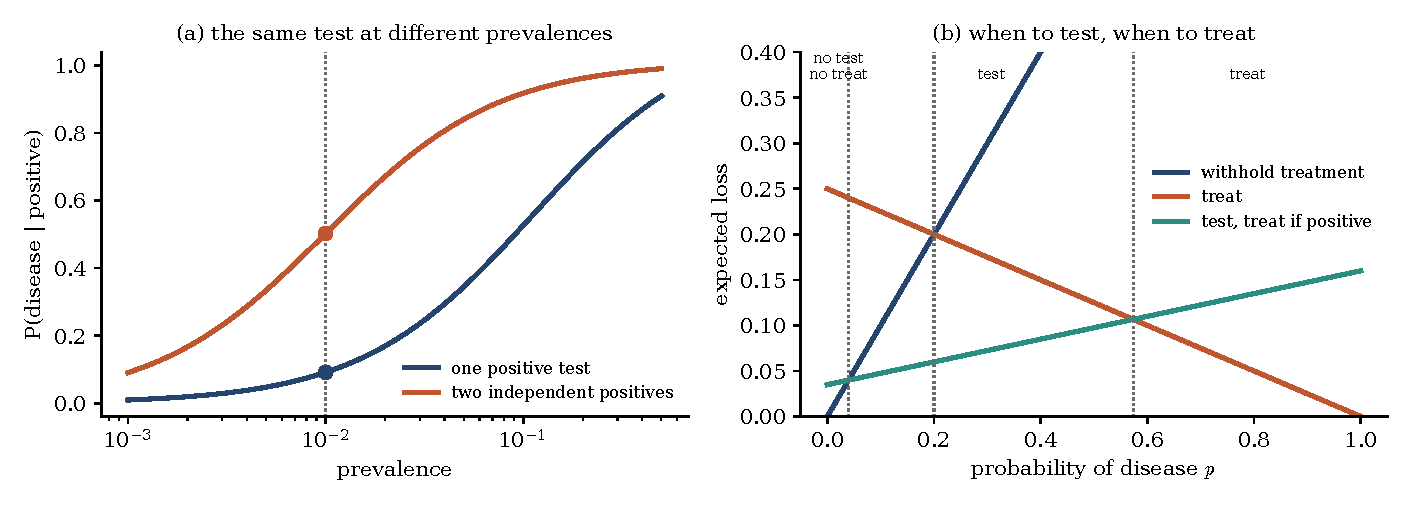
\includegraphics[width=\textwidth]{med_diagnosis}
\caption{(a) Probability of disease after one and two positive results for a test with sensitivity
$0.90$ and false positive rate $0.09$, against prevalence; the points mark prevalence one percent.
(b) Expected loss of withholding treatment, treating, and testing first, against the probability of
disease, for benefit $B=1$, harm $H=0.25$, a test with sensitivity $0.85$ and specificity $0.90$, and
test risk $0.01$; the dotted lines are the three thresholds.}
\label{fig:med_diag}
\end{figure}

\subsection{When to test and when to treat}\label{med:sec:thresholds}

Let $B$ be the net benefit of treating a patient who has the disease and $H$ the net harm of treating
one who does not, in the same units. With probability $p$ of disease, withholding treatment loses
$pB$ in expectation and treating loses $(1-p)H$, so treat if and only if
\[
p>p_t=\frac{H}{H+B}.
\]
This is the Bayes rule of Theorem~\ref{ev:thm:canonical} with prior odds replaced by the patient's
probability and the loss ratio $H/B$ playing the role of $L_{10}/L_{01}$. Pauker and Kassirer (1980)
added a test with sensitivity $\mathrm{se}$, specificity $\mathrm{sp}$ and its own risk $r$. Testing
first and treating the positives loses $p(1-\mathrm{se})B+(1-p)(1-\mathrm{sp})H+r$, and testing is
worth doing on the interval where this beats both alternatives:
\[
p_{\mathrm{low}}=\frac{(1-\mathrm{sp})H+r}{(1-\mathrm{sp})H+\mathrm{se}\,B},\qquad
p_{\mathrm{high}}=\frac{\mathrm{sp}\,H-r}{\mathrm{sp}\,H+(1-\mathrm{se})B}.
\]
Below $p_{\mathrm{low}}$ neither test nor treat; above $p_{\mathrm{high}}$ treat without testing,
because no result could change the decision. With $B=1$, $H=0.25$, $\mathrm{se}=0.85$, $\mathrm{sp}=0.90$
and $r=0.01$, the treatment threshold is $0.20$ and the test is worth ordering for probabilities
between $0.040$ and $0.573$ (Figure~\ref{fig:med_diag}(b)). The test zone shrinks as the test becomes
riskier or less accurate, and vanishes when $r$ exceeds the expected value of the information it
provides, which is the value of information of Section~\ref{med:sec:evpi} for a single patient.

\subsection{Judging a risk model by its decisions}\label{med:sec:dca}

A risk model is usually reported by its area under the ROC curve, which measures ranking and ignores
calibration. Vickers and Elkin (2006) judge it instead by the decisions it supports. Choosing a
treatment threshold $p_t$ declares the harm to benefit ratio $H/B=p_t/(1-p_t)$, from the formula for
$p_t$ above, and the expected utility of treating everyone whose predicted risk exceeds $p_t$, in units
of the benefit of a true positive, is the net benefit
\[
\mathrm{NB}(p_t)=\frac{\mathrm{TP}}n-\frac{\mathrm{FP}}n\cdot\frac{p_t}{1-p_t},
\]
to be compared with treating everyone, $\pi-(1-\pi)p_t/(1-p_t)$ at prevalence $\pi$, and with treating
no one, zero. Figure~\ref{fig:med_dca}(a) uses $200{,}000$ simulated patients with prevalence $0.168$
and two models with the same AUC, $0.781$: the true risk, and an overconfident, shifted transform of it
that ranks patients identically. At $p_t=0.1$ their net benefits are $0.0996$ and $0.0981$ against
$0.0759$ for treating all; at $p_t=0.2$ they are $0.0597$ and $0.0455$; at $p_t=0.3$ they are $0.0359$
and $-0.0011$, so the miscalibrated model is worse than treating no one. AUC cannot see the
difference; the decision curve can. A predictive distribution that is coherent and correctly
specified is calibrated by construction, which is the practical content of the predictive thesis of
Section~\ref{ch:mlprediction} for clinical prediction.

\begin{figure}[H]
\centering
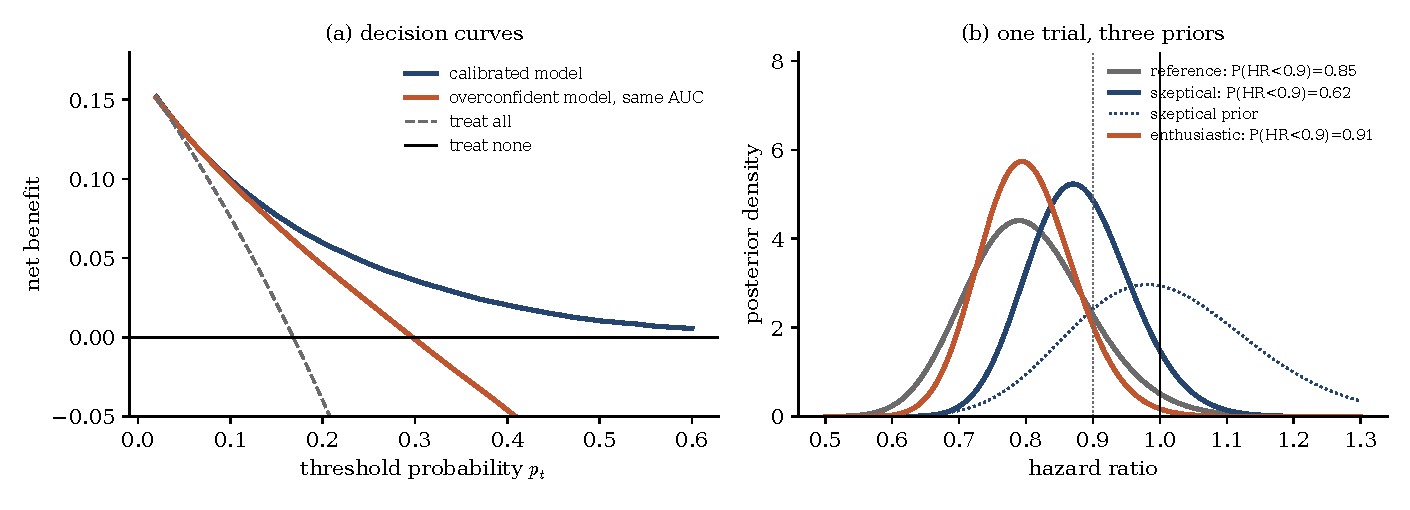
\includegraphics[width=\textwidth]{med_curves_trial}
\caption{(a) Decision curves for a calibrated risk model and an overconfident model with the same AUC,
with the treat all and treat none strategies. (b) Posterior distributions of the hazard ratio from a
trial reporting $0.80$ $(0.64,1.00)$ under reference, skeptical and enthusiastic priors; the dotted
curve is the skeptical prior.}
\label{fig:med_dca}
\end{figure}

\subsection{Reading a trial with a prior}\label{med:sec:priors}

Suppose a trial reports a hazard ratio of $0.80$ with $95$ percent interval $(0.64,1.00)$: on the log
scale an estimate of $-0.223$ with standard error $0.114$, borderline significant. Spiegelhalter,
Freedman and Parmar (1994) recommend reading such a result under a community of priors. A skeptical
prior is centered on no effect, $\log\mathrm{HR}\sim\N(0,0.136^2)$, with spread chosen so that only five
percent of its mass lies below the hoped for hazard ratio of $0.80$; an enthusiastic prior has the
same spread centered on $\log0.80$. Normal updating gives:

\begin{center}\small
\begin{tabular}{lcccc}
\toprule
Prior & posterior HR & $95$ percent interval & $\Pb(\mathrm{HR}<1)$ & $\Pb(\mathrm{HR}<0.9)$\\
\midrule
reference (flat) & $0.80$ & $(0.64,1.00)$ & $0.975$ & $0.850$\\
skeptical & $0.88$ & $(0.74,1.04)$ & $0.933$ & $0.615$\\
enthusiastic & $0.80$ & $(0.67,0.95)$ & $0.995$ & $0.912$\\
\bottomrule
\end{tabular}
\end{center}

\noindent The result convinces an enthusiast and leaves a skeptic with roughly even odds on a
clinically meaningful benefit, taken here as a hazard ratio below $0.9$
(Figure~\ref{fig:med_dca}(b)). The prior skeptic's posterior is the formal version of the instinct
that a single borderline trial should be replicated, and the shrinkage toward one is the correction for
the winner's curse of Section~\ref{ch:screening}. A regulator who wants
the trial to persuade a skeptic can compute in advance the sample size at which it would.

\subsection{An adaptive trial with predictive stopping}\label{med:sec:adaptive}

A single arm phase two trial asks whether a new therapy's response rate exceeds the historical
$p_0=0.2$, with a target of $0.4$ and at most $40$ patients. Following Lee and Liu (2008), put a
uniform prior on the response rate, declare the drug promising at the end if
$\Pb(p>p_0\mid\text{data})>0.95$, which requires at least $13$ responses in $40$, and after $10$, $20$ and
$30$ patients compute the predictive probability that the trial will end in success. Stop for
futility when it falls below $0.05$. The predictive probability is a beta binomial sum over the
unobserved patients, the posterior predictive of Section~\ref{ch:predictive} used as a decision tool.

Simulation with $100{,}000$ trials gives the operating characteristics. If the drug is no better than
the historical rate, it is declared promising in $4.1$ percent of trials, the trial stops early in
$77$ percent, and the expected number of patients is $27.0$. If the true rate is $0.4$, it is declared
promising in $86.0$ percent of trials with $39.2$ patients on average. The fixed design with all $40$
patients has $4.3$ and $87.1$ percent: the adaptive design treats $13$ fewer patients on average with
an ineffective drug for one point of power. Futility stopping can only remove rejections, so the false
positive rate cannot exceed that of the fixed design; that is the validity layer of
Figure~\ref{fig:tst_layers}, and the predictive probability is the decision layer.
Figure~\ref{fig:med_trial}(a) gives the full operating characteristic curve.

\begin{figure}[H]
\centering
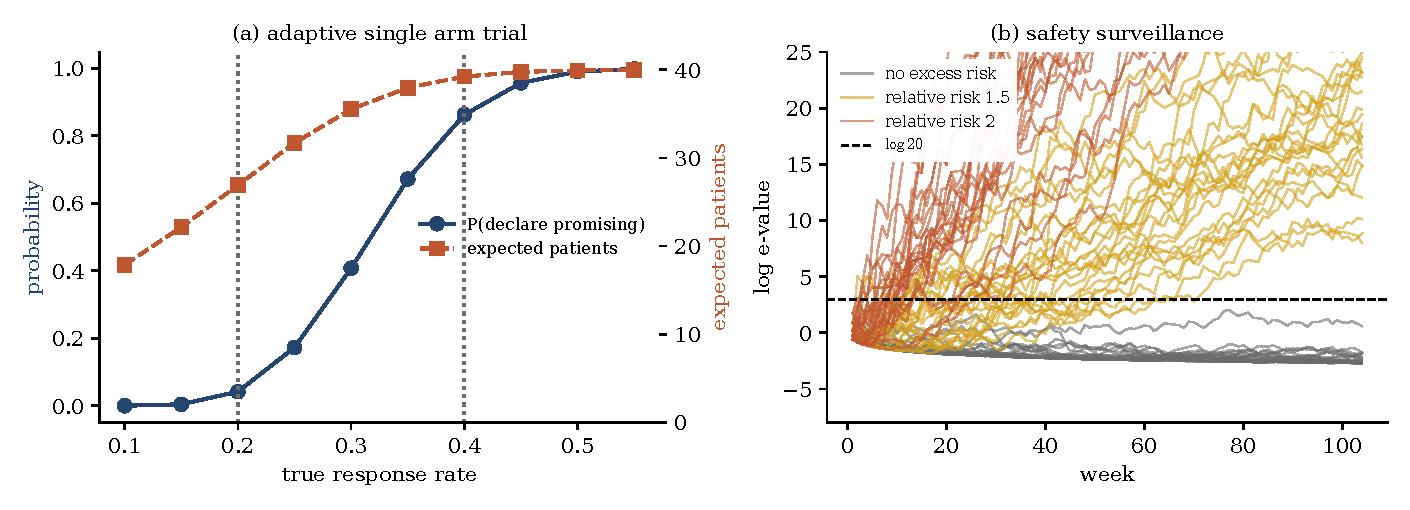
\includegraphics[width=\textwidth]{med_trial_surveillance}
\caption{(a) Probability of declaring the drug promising and expected number of patients against the
true response rate, for the predictive probability design. (b) Twenty five paths of the log mixture
e-value for weekly adverse event counts under no excess risk and under relative risks $1.5$ and $2$,
with the alarm threshold $\log20$.}
\label{fig:med_trial}
\end{figure}

\subsection{Continuous safety surveillance}\label{med:sec:surveillance}

After a vaccine or drug is licensed, reports of a specific adverse event arrive weekly, and the
question is whether they exceed the background rate. Looking every week is the point, so a test that
is valid only at a fixed sample size is the wrong tool. Let weekly counts be Poisson with mean
$\rho\lambda_0$, background $\lambda_0=2$, and put a $\mathrm{Gamma}(1,1)$ prior on the relative risk
$\rho$. The Bayes factor of the mixture against $\rho=1$ is a null martingale (Section~\ref{ch:evalues}),
so raising an alarm when it first exceeds $20$ has false alarm probability at most $0.05$ over an
unlimited horizon. Over two years of weekly looks, $20{,}000$ simulated surveillance runs give a false
alarm rate of $2.2$ percent with no excess risk. With relative risk $1.5$ the alarm sounds in $99.9$
percent of runs, at median week $22$; with relative risk $2$ at median week $7$
(Figure~\ref{fig:med_trial}(b)). The maximized sequential probability ratio test used in vaccine
surveillance (Kulldorff and coauthors, 2011) maximizes over the relative risk instead of averaging, and
needs a separately computed critical value to restore its error rate, the generalized likelihood
ratio problem of Section~\ref{ch:testpractice}; the mixture needs none.

\subsection{What is further research worth?}\label{med:sec:evpi}

Suppose the evidence on a new treatment gives a posterior for its incremental net benefit per patient,
in quality adjusted life years, of $\N(m,s^2)$ with $m=0.05$ and $s=0.10$. Adopting it is the Bayes
decision because $m>0$, though the probability that it is actually better is only $\Phi(m/s)=0.69$.
Perfect information would let the decision maker adopt only when the benefit is positive, so the
expected value of perfect information per patient is
\[
\mathrm{EVPI}=\E[\max(\theta,0)]-\max(\E\theta,0)=s\,\phi(m/s)+m\,\Phi(m/s)-\max(m,0)=0.0198,
\]
and over $10^5$ future patients about $1980$ quality adjusted life years. That is an upper bound on
what any further trial is worth; a trial that costs more, in money converted at the decision maker's
willingness to pay, should not be run however uncertain the result looks. Claxton (1999) called this
the irrelevance of inference: the adoption decision follows the posterior mean, and the uncertainty
enters only through the value of collecting more data. It is the Bayes risk calculus of
Section~\ref{ch:risk} applied to research funding.

\subsection{A case study: modal doctor, Bayesian patient}\label{med:sec:cancer}

The threads of this section meet in a single patient. In autumn 2004 a 55 year old social scientist,
Patient A in the account of Polson and Sokolov (2026b), was diagnosed with localized prostate cancer: Gleason 6,
stage T1b, PSA 1.9. His urologists offered open radical prostatectomy with extended pelvic lymph node
dissection by a very experienced surgeon, robotic prostatectomy without nodal dissection by a less
experienced one, or external beam radiation. He computed his own discounted quality adjusted life
expectancy under each option and sent the calculation to a physician colleague asking what he was
missing. The correspondence raises three questions that this book can answer formally.

\paragraph{The prior is itself uncertain.} The Partin nomogram gave point probabilities
$\hat\pi=(0.61,0.35,0.02,0.02)$ for organ confined disease, capsular penetration, seminal vesicle
involvement and lymph node involvement, with a footnote that each was accurate to within ten points
only in a stated fraction of cases. A published prediction with a stated accuracy is a prior over the
prior. Put $\pi_k\sim\mathrm{Beta}(\alpha_k,\beta_k)$ with mean $\hat\pi_k$ and choose the effective
sample size $n_k=\alpha_k+\beta_k$ to match the calibration statement. For the 2026 nomogram,
$\mathrm{Beta}(26,7)$ for organ confined disease has $\Pb(|\pi-0.78|\le0.10)=0.845$ and
$\mathrm{Beta}(4,16)$ for capsular penetration has $0.752$, matching the stated $0.85$ and $0.75$. For a
rare state the matching fails: with $\hat\pi=0.01$ an interval of ten points is nearly certain for every
Beta with that mean, its probability falling from $0.990$ for a very diffuse Beta to $0.972$ at
$n_k\approx3.6$ and rising to one for a very concentrated one, so the equation has no solution at a
stated accuracy below $0.972$, two between $0.972$ and $0.990$, and one above. The
remedy is to anchor a quantile of the Beta at the clinical threshold that would change management,
$5$ percent for nodal dissection. Requiring the $97.5$th percentile to equal $0.05$ gives
$\mathrm{Beta}(0.494,48.9)$; the $95$th percentile gives the more diffuse $\mathrm{Beta}(0.225,22.3)$ and
the $99$th the more concentrated $\mathrm{Beta}(0.827,81.9)$. Figure~\ref{fig:med_cancer}(a) shows the
upper tails. The mean is $0.01$ in every case; what changes is the mass above the threshold, $5$, $2.5$
and $1$ percent, and that is what a risk averse patient pays attention to. (A $\mathrm{Beta}(1,99)$ has
the same mean but puts only $0.6$ percent above $0.05$; its $97.5$th percentile is $0.037$. For the 2004
estimate $\hat\pi=0.02$ the $97.5$ percent anchor gives $\mathrm{Beta}(2.61,127.7)$.)

\paragraph{The doctor uses the mode, the patient the posterior.} Patient A wrote that doctor and
patient were in the same place about ``decisions by the mode and decisions at the extreme'';
his colleague replied that physicians are taught to think in population terms. Formally, the maximum
a posteriori rule chooses the best action for the most likely state, here organ confined disease, where
nodal dissection only adds morbidity, while the Bayes rule averages over states. With an aggressive
action $a_+$ and a conservative one $a_-$, a tail state of probability $\pi_{\mathrm{tail}}$ in which
$a_+$ gains $\Delta U_{\mathrm{tail}}$, and a certain morbidity cost $\Delta C$ of $a_+$ at the mode,
\[
\E_\pi[U(\theta,a_+)-U(\theta,a_-)]\ \ge\ \pi_{\mathrm{tail}}\,\Delta U_{\mathrm{tail}}-\Delta C ,
\]
when $a_+$ is at least as good as $a_-$ in every state other than the mode. The two rules part
company when $\kappa=\Delta U_{\mathrm{tail}}/\Delta C$ exceeds $1/\pi_{\mathrm{tail}}$ (Figure~\ref{fig:med_cancer}(b)). Patient A's own numbers
were a $2$ percent chance of nodal involvement, a missed nodal branch worth $8$ to $12$ discounted
QALYs against about $21.3$ if cured, and a dissection morbidity of $0.05$ to $0.10$ QALYs. The tail gain
$0.02\times(21.3-10)\approx0.23$ QALYs exceeds the morbidity cost across the whole range, and $\kappa$
lies between $93$ and $266$, well above $1/\pi_{\mathrm{tail}}=50$: the Bayes action was surgery with
dissection although the modal state recommended against it. This is the treatment threshold of
Section~\ref{med:sec:thresholds} read in reverse, with $H=\Delta C$, $B=\Delta U_{\mathrm{tail}}$ and
$p_t=\Delta C/(\Delta C+\Delta U_{\mathrm{tail}})\approx0.007$, far below $0.02$. Andrew Grove,
facing the same diagnosis in 1995, weighted surgical morbidity heavily and chose brachytherapy;
under his utility the same calculation places him below the curve, and both choices are Bayes actions
for their owners.

\paragraph{Some treatments destroy information.} Patient A's handwritten note reads ``radiation, no
surgery afterwards, hence learn no information''. Surgery with nodal dissection stages the disease
almost exactly; radiation forecloses later staging. In a two stage problem the value of an action is
its direct utility plus the discounted expected value of the best second stage decision under the
posterior it leaves behind, and because $\pi\mapsto\max_{a'}\E_\pi U_2(\cdot,a')$ is convex, Jensen's
inequality makes that option value nonnegative and positive whenever some possible finding would
change the second decision. Standard cost utility analysis counts only the direct term and so
undervalues actions that yield information. A modern version is staging by PSMA PET before choosing
between the two operations. With sensitivity $0.80$ and specificity $0.995$ the scan has likelihood
ratios $160$ and $0.20$, so a prior nodal probability of $0.01$ becomes $0.62$ after a positive scan and
$0.002$ after a negative one. Taking the loss of $a_+$ as $\Delta C=0.075$ and the loss of $a_-$ as
$\pi\,\Delta U_{\mathrm{tail}}$ with $\Delta U_{\mathrm{tail}}=11.3$, the scan is worth $0.051$ QALYs,
about $19$ quality adjusted days, at prior $0.01$, and $10$ days at prior $0.02$; it is worth most,
about $21$ days, near prior $0.007$, where the decision is closest to a coin flip, and nothing above
about $0.033$, where no negative scan could bring the posterior below the threshold
(Figure~\ref{fig:med_cancer}(c)). That is the Pauker and Kassirer testing zone again, now with a test
that is itself a treatment choice.

\begin{figure}[H]
\centering
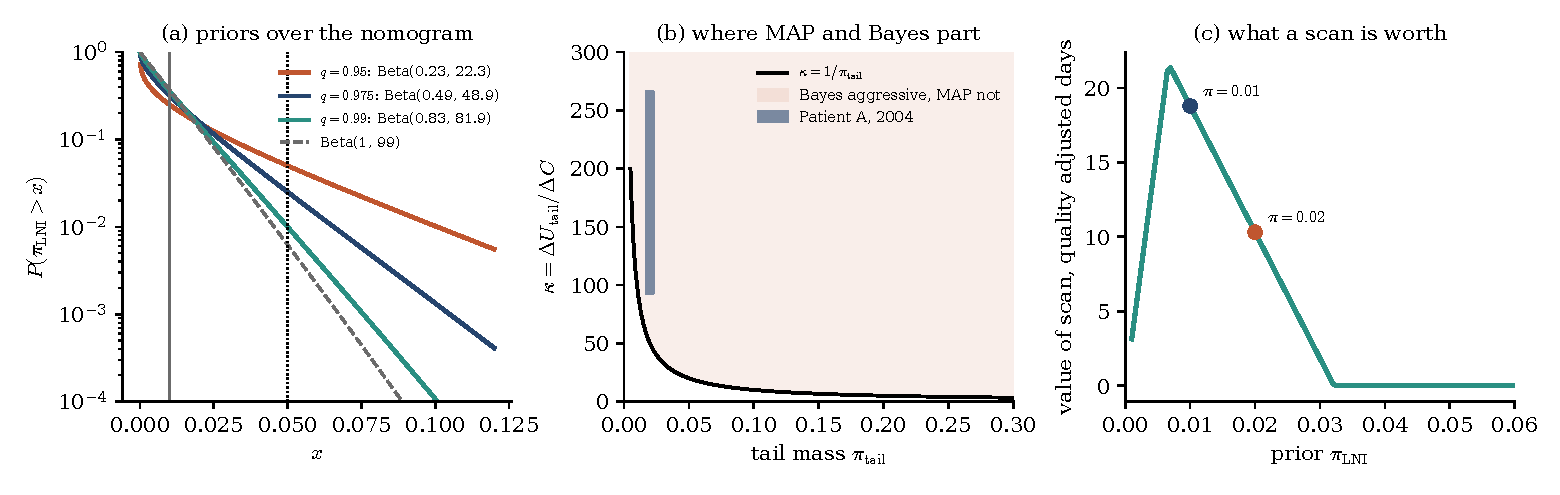
\includegraphics[width=\textwidth]{med_cancer_case}
\caption{The prostate cancer case. (a) Upper tails of Beta priors for the nodal involvement
probability with mean $0.01$, anchored at the $95$th, $97.5$th and $99$th percentile equal to the $5$
percent threshold, and $\mathrm{Beta}(1,99)$. (b) The region where the Bayes rule prefers the
aggressive action and the modal rule does not, with Patient A's 2004 range. (c) Value of a PSMA PET
scan before choosing between prostatectomy with and without nodal dissection, against the prior
probability of nodal involvement.}
\label{fig:med_cancer}
\end{figure}

\paragraph{Discounting and the 2026 decision.} Patient A's $21.3$ QALYs is thirty years at quality
weight $0.95$ discounted at $2$ percent a year, $0.95\times(1-1.02^{-30})/0.02=21.28$; at weight
$0.90$ the same formula gives $20.16$. A QALY thirty years out is worth $0.55$ of one today at $2$
percent, $0.36$ at the $3.5$ percent required by NICE, and $0.23$ at $5$ percent. Because the losses
that nodal dissection prevents arrive late, a health system discounting at $5$ percent sees a smaller
advantage for the aggressive action than a patient discounting at $2$ percent, a second source of
disagreement between doctor and patient that has nothing to do with the posterior. For the same
patient in 2026, Polson and Sokolov report from a calibrated multistate simulation (not reproduced
here) posterior expected discounted QALYs of $21.46$ for active surveillance, $21.35$ for prostatectomy
without nodes, $21.33$ for focal HIFU, $21.26$ for prostatectomy with nodes and $20.27$ for radiation
with androgen deprivation. Active surveillance, with escalation on biopsy or imaging progression, is
now the Bayes action for low risk disease, which is current guideline practice; the gap to surgery
narrows as risk aversion rises, so a patient with a strong premium on certainty, as Patient A had, can
still rationally choose surgery. The three structural points of the 2004 letter survive the change of
action set: the prior is uncertain, the mode is not the posterior, and actions differ in the
information they leave behind.

\paragraph{Summary.} Posterior odds are prior odds times the likelihood ratio, and prevalence is the
prior; the treatment threshold is $H/(H+B)$, and tests are worth ordering only between two further
thresholds; a risk model should be judged by net benefit, which sees calibration that AUC cannot; a
trial should be read under skeptical and enthusiastic priors; predictive probabilities let a trial stop
early without inflating its error rate; mixture e-values allow continuous safety monitoring; and the
value of information prices further research. In a single patient all of these combine: a calibrated
prior over the nomogram, the Bayes rule rather than the modal rule, and credit for actions that leave
information behind.

\subsection*{Problems}
\begin{enumerate}[leftmargin=2.2em,itemsep=2pt]
\item Recompute the mammography numbers, and find the prevalence at which a positive result makes
cancer more likely than not.
\item Derive the Pauker and Kassirer thresholds $p_{\mathrm{low}}$ and $p_{\mathrm{high}}$, and find
the test risk $r$ at which the testing zone vanishes in the example.
\item Show that net benefit at threshold $p_t$ equals, up to a positive factor, the expected utility of
the decision rule ``treat if predicted risk exceeds $p_t$'' when $H/B=p_t/(1-p_t)$, and explain why a
monotone transform of a calibrated model keeps its AUC but loses net benefit.
\item For the trial example, find the sample size, with the same estimated effect, at which the skeptical
posterior gives $\Pb(\mathrm{HR}<0.9)>0.9$.
\item Write the predictive probability of final success as a beta binomial sum and reproduce the
operating characteristics of the adaptive design; add an efficacy stop and check the false positive
rate.
\item Prove that the Gamma mixture Bayes factor in the surveillance example is a martingale under no
excess risk, and compare its alarm times with those of a maximized likelihood ratio that is not.
\item Derive the closed form of the EVPI for a normal posterior and show that it is largest when $m=0$.
\item For the nomogram prior with mean $0.01$, show that the equation $\Pb(|\pi-0.01|\le0.10)=c$ in
the effective sample size has no solution for $c<0.972$, two for $0.972<c<0.990$ and one for
$0.990\le c<1$, and solve the quantile anchoring equation for the $97.5$th
percentile.
\item Prove the wedge bound for the modal and Bayes rules, and find the range of morbidity costs over
which Patient A's Bayes action is surgery with nodal dissection.
\item Reproduce the value of the PSMA PET scan as a function of the prior, and find the two prior
probabilities at which it vanishes.
\end{enumerate}

\src{Gigerenzer, Gaissmaier, Kurz-Milcke, Schwartz and Woloshin (2007); Pauker and Kassirer (1980);
Vickers and Elkin (2006); Spiegelhalter, Freedman and Parmar (1994); Spiegelhalter, Abrams and Myles
(2004); Lee and Liu (2008); Berry (2006); Berry, Carlin, Lee and M\"uller (2010); Kulldorff, Davis, Kolczak, Lewis, Lieu and Platt (2011);
Claxton (1999); Parmigiani and Inoue (2009); Polson and Sokolov, ``Modal Doctor, Bayesian Patient: A Case Study in Cancer
Treatment'' (2026b), whose Table~3 values are quoted and whose remaining numbers were recomputed (the
anchored Beta for the 2026 nodal prior is $\mathrm{Beta}(0.494,48.9)$ rather than $\mathrm{Beta}(1,99)$,
the 2004 prior with mean $0.02$ is $\mathrm{Beta}(2.61,127.7)$, and the stated PSMA PET accuracy gives a
positive predictive probability of $0.62$ rather than $0.67$); Partin and coauthors (1997) and Eifler and coauthors (2013) on the Partin tables; Grove
(1996). The trial, risk model and surveillance data are simulated; all other numbers were computed for
the book.}


\shorthead{Twenty One Bayesian Vignettes}
\section{Applications in Practice: Twenty One Bayesian Vignettes}\label{ch:vignettes}

\noindent\textbf{Thesis.} Each vignette below is a self contained application of the predictive apparatus of this
book, drawn from decision and prediction problems, hierarchical modeling, model criticism,
nonparametric Bayes, and the applied sciences. In every case the model returns a full posterior, that posterior is read as a
distribution over consequences, and a decision follows by averaging a loss against it. The
figures are generated by the accompanying code, with fixed seeds, so every quoted number is
reproducible.

\subsection{A/B testing and the shipping decision}
A product team runs an experiment: variant A converts $80$ of $400$ visitors and variant B
converts $95$ of $400$. With independent uniform priors the posteriors are
$\theta_A\sim\mathrm{Beta}(81,321)$ and $\theta_B\sim\mathrm{Beta}(96,306)$, drawn in
Figure~\ref{fig:app_abtest}(a). What matters for the decision is not either rate but the
uplift $\delta=\theta_B-\theta_A$, whose posterior in panel (b) places
$\Pr(\delta>0\mid\text{data})\approx0.90$ with a posterior mean near $3.7$ percentage points.
Under a symmetric loss the team ships B; under a loss that penalizes a wrongful switch more
than a missed gain, the same posterior returns the expected regret of each action directly.
This is the predictive decision loop of the book in miniature: a Beta Binomial update
followed by an expected loss comparison, with no appeal to a null hypothesis.\index{A/B testing}

\begin{figure}[H]
\centering
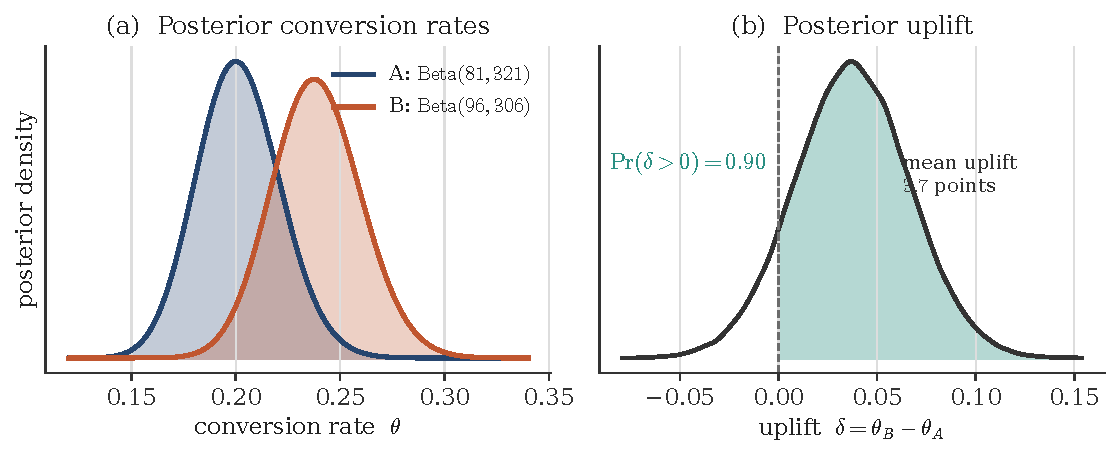
\includegraphics[width=0.9\textwidth]{app_abtest}
\caption{A/B testing as Bayesian decision. (a) Posterior conversion rates for the two
variants. (b) Posterior of the uplift $\delta=\theta_B-\theta_A$; the shaded mass is
$\Pr(\delta>0\mid\text{data})\approx0.90$. The decision reads the loss against panel (b), not
against a significance threshold.}
\label{fig:app_abtest}
\end{figure}

\subsection{Borrowing strength: hierarchical shrinkage}
Twelve groups, whether clinics, teams, or web variants, each report a success rate from a
modest sample, and the raw rates $y_i/n_i$ scatter widely with much of the spread being noise.
A hierarchical model with a common mean pools them: each posterior mean is drawn toward the
grand mean by an amount set by its own sample size, so the smallest and noisiest groups are pooled
hardest. Figure~\ref{fig:app_shrinkage} places the unpooled estimates on the left and the
partially pooled posterior means on the right, with the connecting segments showing the
shrinkage. This is the lesson of Stein and of the global local priors earlier in the book:
the group level predictive borrows strength from its neighbors, and the pooled rule dominates
the unpooled one in aggregate risk.\index{hierarchical model}\index{shrinkage}

\begin{figure}[H]
\centering
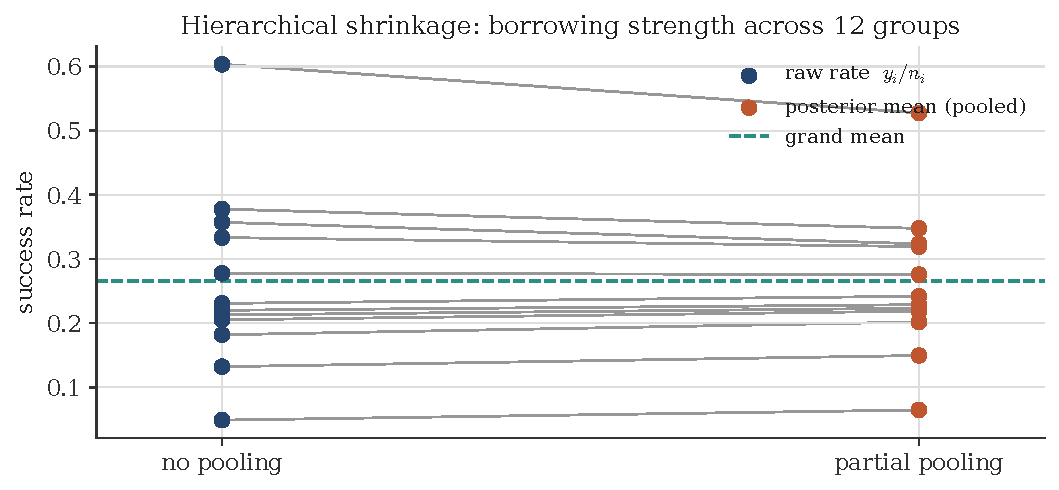
\includegraphics[width=0.9\textwidth]{app_shrinkage}
\caption{Hierarchical shrinkage across twelve groups. Unpooled rates (left) are pulled toward
the grand mean (dashed) to give the partially pooled posterior means (right); small samples
are pooled hardest. Pooling trades a little bias for a large variance reduction.}
\label{fig:app_shrinkage}
\end{figure}

\subsection{Nonparametric regression with Gaussian processes}
Given eight noisy observations of an unknown function, a Gaussian process prior with a
squared exponential kernel yields a closed form posterior over functions.
Figure~\ref{fig:app_gp} shows the posterior mean, three posterior sample paths, and the
pointwise $95\%$ credible band, which widens where data are scarce and pinches at the
observations. The band is the honest expression of what the predictive does not yet know, and
the truth $\sin x$ lies inside it throughout. This is the function space reading of de Finetti
developed in the nonparametric material: exchangeable observations of a surface, integrated
against a prior over surfaces.\index{Gaussian process}

\begin{figure}[H]
\centering
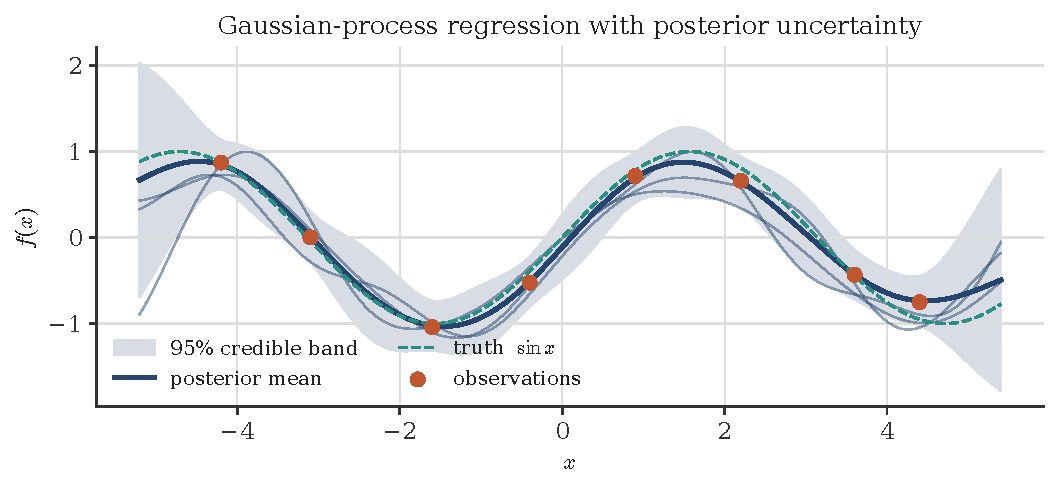
\includegraphics[width=0.9\textwidth]{app_gp}
\caption{Gaussian process regression. Posterior mean (solid), three posterior draws (thin),
and the $95\%$ credible band, from eight noisy observations. Uncertainty grows away from the
data and contracts at it; the band, not the mean, is the inferential object.}
\label{fig:app_gp}
\end{figure}

\subsection{Recursive estimation: the Kalman filter}
A moving object is tracked from noisy position readings. The Kalman filter is exact Bayesian
updating in a linear Gaussian state space model: at each step the prior is propagated forward,
the new reading tilts it, and the posterior mean is a precision weighted average of prediction
and observation. Figure~\ref{fig:app_kalman} shows the readings, the true trajectory, and the
filtered posterior mean with its $95\%$ band. The filter is the sequential predictive of the
book run one datum at a time, and its gain is the posterior weight each new
observation earns.\index{Kalman filter}\index{state space model}

\begin{figure}[H]
\centering
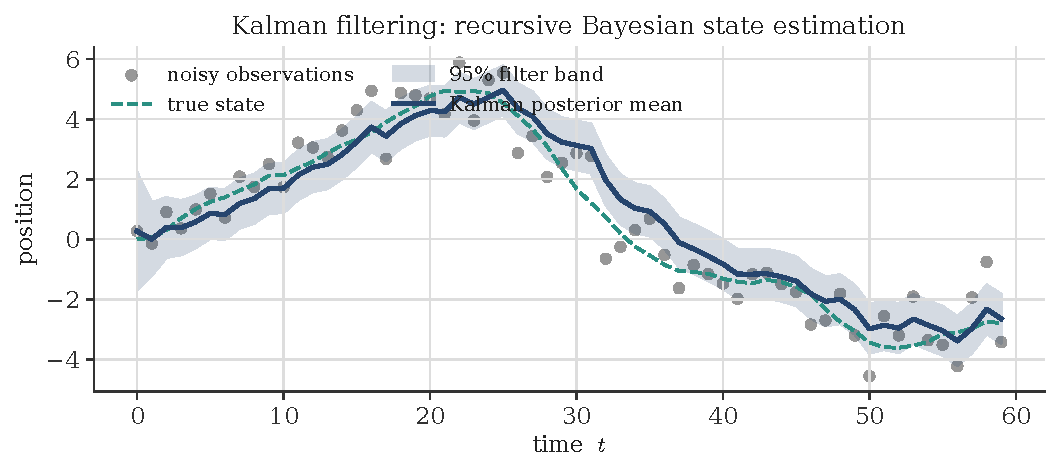
\includegraphics[width=0.9\textwidth]{app_kalman}
\caption{Kalman filtering as recursive Bayes. Noisy observations (gray), true state (dashed),
and the filtered posterior mean with its $95\%$ band. Each update is a conjugate Gaussian step;
the Kalman gain is the posterior weight on the new datum.}
\label{fig:app_kalman}
\end{figure}

\subsection{Exploration and the multiarmed bandit}
Three actions have unknown success probabilities near $0.50$, $0.55$, and $0.60$. Thompson
sampling acts by drawing a parameter from the posterior and playing its best arm, so
exploration is automatic: an arm is tried in proportion to its posterior probability of being
optimal. Figure~\ref{fig:app_bandit} compares the cumulative regret of Thompson sampling, UCB,
and $\varepsilon$-greedy over $1500$ rounds, averaged over $200$ replications with
two standard error bands. Thompson sampling has the lowest regret of the three: at round $1500$
its mean regret is $25.0$, against $37.1$ for $\varepsilon$-greedy, whose fixed exploration keeps
paying a linear tax, and $48.6$ for UCB, whose exploration bonus is large against gaps of $0.05$
to $0.10$. Here the posterior is
not an input to the policy; it \emph{is} the policy.\index{Thompson sampling}\index{multiarmed bandit}

\begin{figure}[H]
\centering
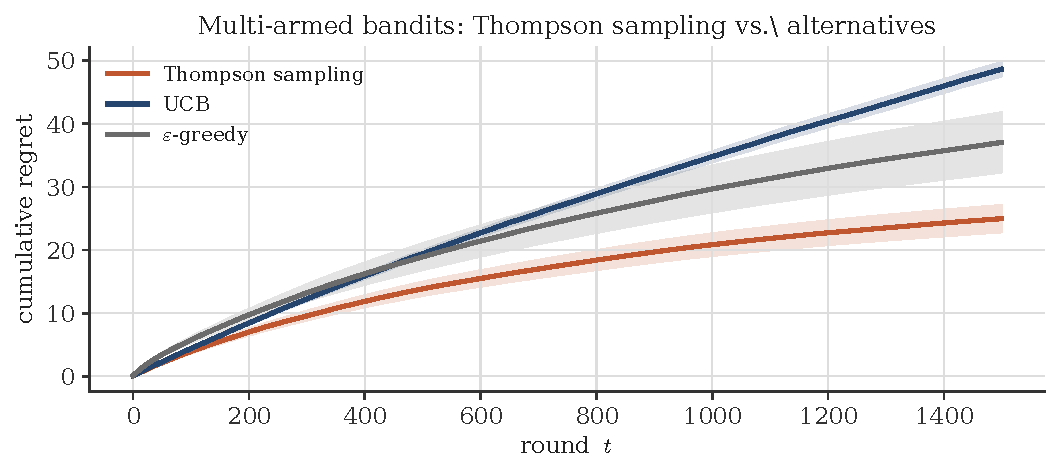
\includegraphics[width=0.9\textwidth]{app_bandit}
\caption{Regret in a three armed bandit. Cumulative regret for Thompson sampling, UCB, and
$\varepsilon$-greedy, averaged over $200$ runs with two standard error bands. Posterior driven
exploration beats both the optimism benchmark and fixed exploration.}
\label{fig:app_bandit}
\end{figure}

\subsection{Detecting a change: Bayesian change point analysis}
A monitored series shifts its mean at an unknown time. Placing a flat prior over the
change point location and scoring each split by its profile likelihood, with the mean and variance of each segment set to their maximum likelihood estimates, gives an approximate posterior over the location
directly. Figure~\ref{fig:app_changepoint} shows the series with its true break at $t=48$ and,
below it, the posterior $\Pr(\tau=t\mid y)$ of the change point $\tau$, which concentrates sharply with a mode at
$\hat\tau=48$. The posterior is not a point estimate but a distribution over explanations, and
its spread is the analyst's honest uncertainty about when the world changed. This is the
evidence comparison of the book applied across every candidate
split, with the profile likelihood standing in for the marginal likelihood.\index{change point detection}

\begin{figure}[H]
\centering
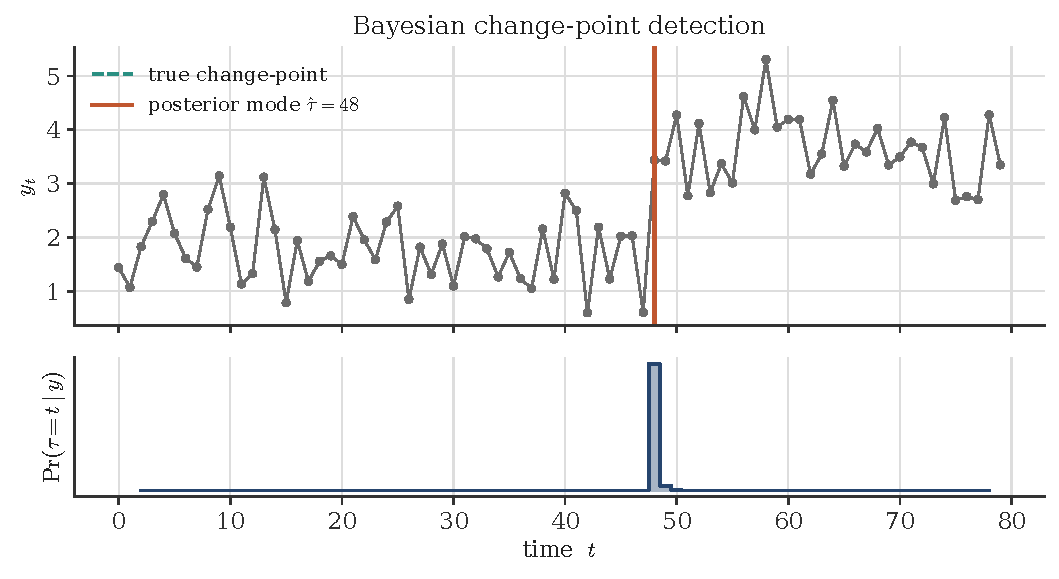
\includegraphics[width=0.9\textwidth]{app_changepoint}
\caption{Bayesian change point detection. Top: the series with true break (dashed) and
posterior mode (solid). Bottom: the posterior over the change point location, which
concentrates at the truth. The output is a distribution over when, not merely an estimate.}
\label{fig:app_changepoint}
\end{figure}


\subsection{Eight schools: the canonical hierarchical model}
Eight schools run the same coaching program; each reports an estimated effect with its own
standard error, ranging from $+28$ points to $-3$. Taken at face value the spread suggests the
program works wonderfully in school A and backfires in school C. The hierarchical model
treats the eight true effects as exchangeable draws from a population with mean $\mu$ and
between school spread $\tau$, and lets the data decide how much the schools really differ.
Figure~\ref{fig:app_eightschools}(a) shows the result: the posterior intervals are pulled
sharply toward the population mean, school A's headline $28$ shrinking to about $11$, and every
interval tightening as it borrows strength from the other seven. Panel (b) explains why. The
posterior for $\tau$ piles up near zero, so the data are consistent with the schools being
nearly identical and the apparent spread being noise. Nothing here is an ad hoc correction for
multiplicity; the shrinkage is what Bayes returns once the schools are modeled as
exchangeable.\index{hierarchical model}\index{eight schools}\index{exchangeability}

\begin{figure}[H]
\centering
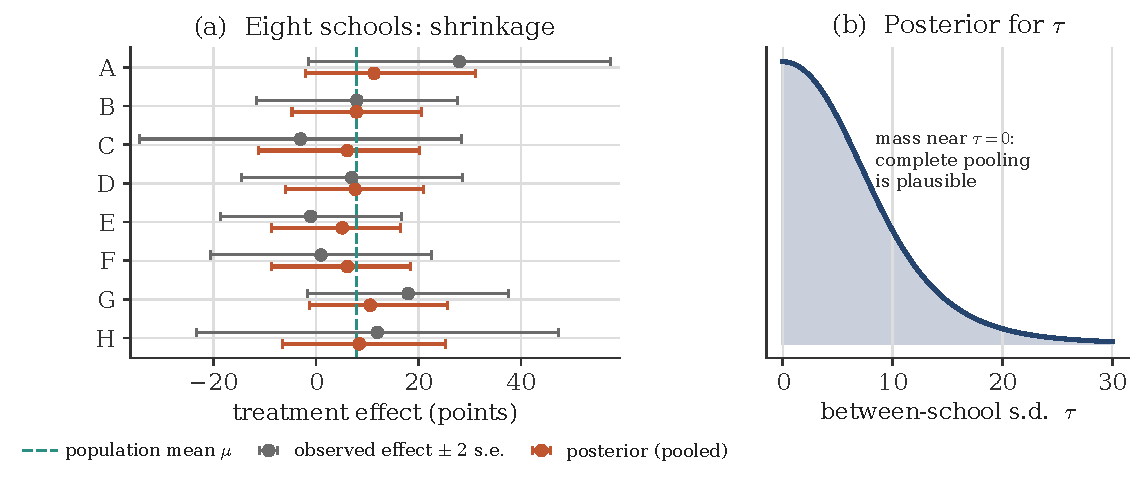
\includegraphics[width=0.9\textwidth]{app_eightschools}
\caption{The eight schools hierarchical model. (a) Observed effects with two standard error
bars, against posterior intervals that shrink toward the population mean (dashed). (b) The
posterior for the between school standard deviation $\tau$, whose mass near zero is what drives
the pooling.}
\label{fig:app_eightschools}
\end{figure}

\subsection{The funnel: when geometry defeats the sampler}
Hierarchical models carry a hazard that is invisible in the algebra and obvious in a picture.
Plotting a school effect $\theta_1$ against $\log\tau$ in
Figure~\ref{fig:app_funnel}(a) produces the funnel: as $\tau$ shrinks the conditional spread of
$\theta_1$ collapses, so the posterior narrows to a cusp that a sampler tuned for the wide part
of the space cannot enter. The cure is a change of variable. Writing
$\theta_j=\mu+\tau\eta_j$ and sampling the standardized $\eta_j$ gives panel (b), where the
geometry is nearly spherical and the same sampler mixes freely. The two panels are the same
posterior in different coordinates, which is the practical face of the parametrization
dependence discussed in Chapter~\ref{chap:asymptotics}: curvature, not the model, is what makes
computation hard.\index{funnel}\index{noncentered parametrization}\index{reparametrization}

\begin{figure}[H]
\centering
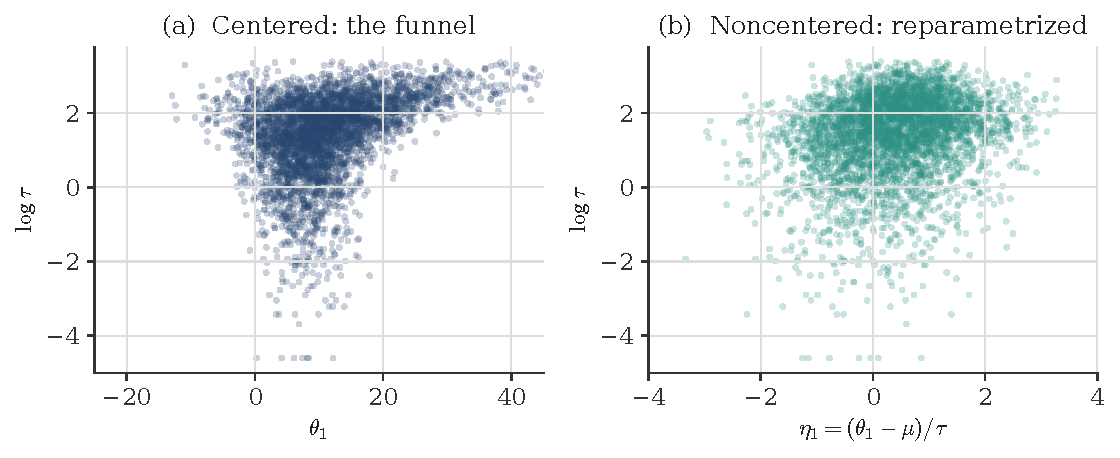
\includegraphics[width=0.9\textwidth]{app_funnel}
\caption{The hierarchical funnel. (a) In the centered parametrization the posterior narrows as
$\tau\to0$, creating a region samplers struggle to explore. (b) The noncentered coordinates
$\eta_j=(\theta_j-\mu)/\tau$ remove the pathology. Same posterior, different geometry.}
\label{fig:app_funnel}
\end{figure}

\subsection{Posterior predictive checks: letting the model fail visibly}
A Bayesian model that fits badly should say so, and the posterior predictive is where it
confesses. Counts are fitted with a Poisson likelihood, whose mean and variance are forced to
be equal, when the truth is overdispersed. Drawing replicate data sets from the posterior
predictive and overlaying them on the observed histogram,
Figure~\ref{fig:app_ppc}(a) already shows the replicates too tightly concentrated. Panel (b)
makes it quantitative by choosing a discrepancy the model cannot fake, the variance to mean
ratio: the observed value sits far outside the entire predictive distribution, giving a
predictive $p$-value below $0.001$. The check is not a test of a null hypothesis but a
comparison of the observed world with the worlds the fitted model believes in.\index{posterior
predictive check}\index{model criticism}\index{overdispersion}

\begin{figure}[H]
\centering
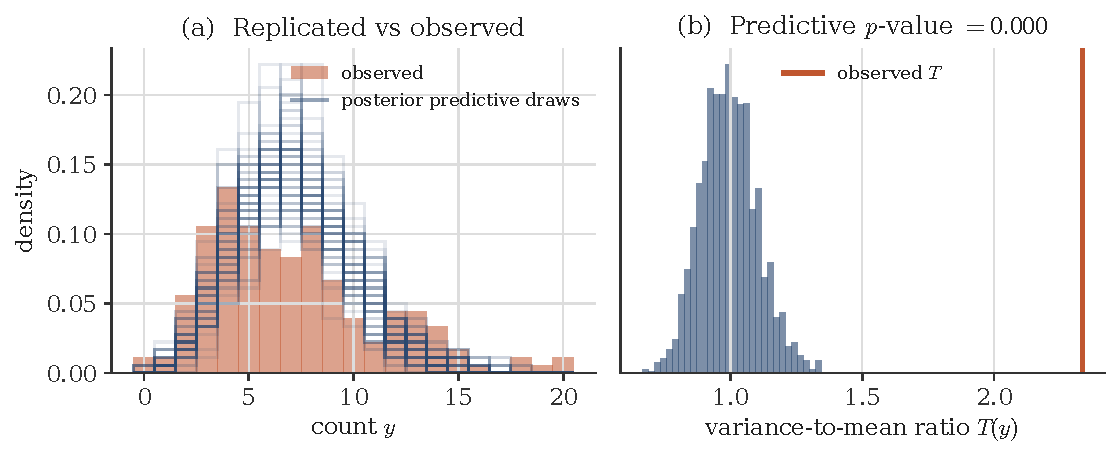
\includegraphics[width=0.9\textwidth]{app_ppc}
\caption{A posterior predictive check that fails. (a) Replicated data sets from a fitted
Poisson model against the observed counts. (b) The observed variance to mean ratio lies outside
the predictive distribution, exposing the overdispersion the model cannot represent.}
\label{fig:app_ppc}
\end{figure}

\subsection{Reading MCMC output: mixing, convergence, and $\hat R$}
Posterior summaries are only as trustworthy as the sampler that produced them, and two plots
diagnose most of what goes wrong. Figure~\ref{fig:app_mcmc}(a) traces four chains started from
deliberately dispersed points; they forget their starting values and settle into a common band,
the visual signature of mixing. Panel (b) tracks the running mean of each chain, which converges
to the target value from every start. The numerical summary is the potential scale reduction
factor, here $\hat R\approx1.01$: the between chain and within chain variances agree, so the
chains are exploring the same distribution. Had the funnel of an earlier vignette been left
uncured, these diagnostics are what would have caught it.\index{MCMC}\index{convergence
diagnostics}\index{Gelman Rubin statistic}

\begin{figure}[H]
\centering
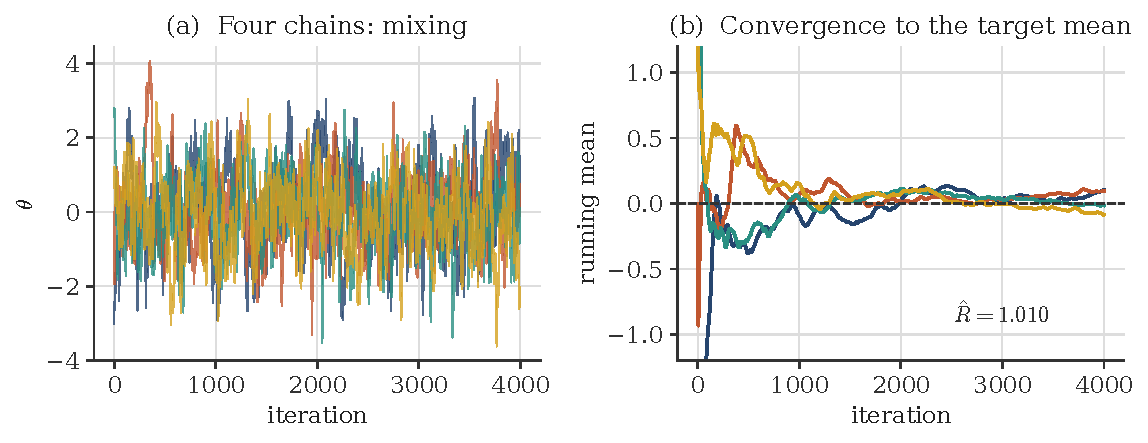
\includegraphics[width=0.9\textwidth]{app_mcmc}
\caption{MCMC diagnostics. (a) Four chains from dispersed starting values mixing into a common
band. (b) Running means converging to the target, with $\hat R\approx1.01$ confirming that
between chain and within chain variation agree.}
\label{fig:app_mcmc}
\end{figure}

\subsection{Bayesian logistic regression and the calibration of a predictive}
A binary outcome is modeled by logistic regression with a Gaussian prior on the coefficients.
Figure~\ref{fig:app_logistic}(a) shows the posterior for the two slopes, each concentrating
around the value used to generate the data, and the width of those posteriors is the honest
statement of what six hundred observations can resolve. Panel (b) asks the question that
matters for use: when the model says $30\%$, does the event happen about $30\%$ of the time?
Plotting observed frequency against predicted probability, with a predictive band for binomial
noise, the curve tracks the diagonal within the band. This is calibration in the sense of the
scoring rule material earlier in the book, and it is the property that licenses feeding these
probabilities into a decision rule.\index{logistic regression}\index{calibration}

\begin{figure}[H]
\centering
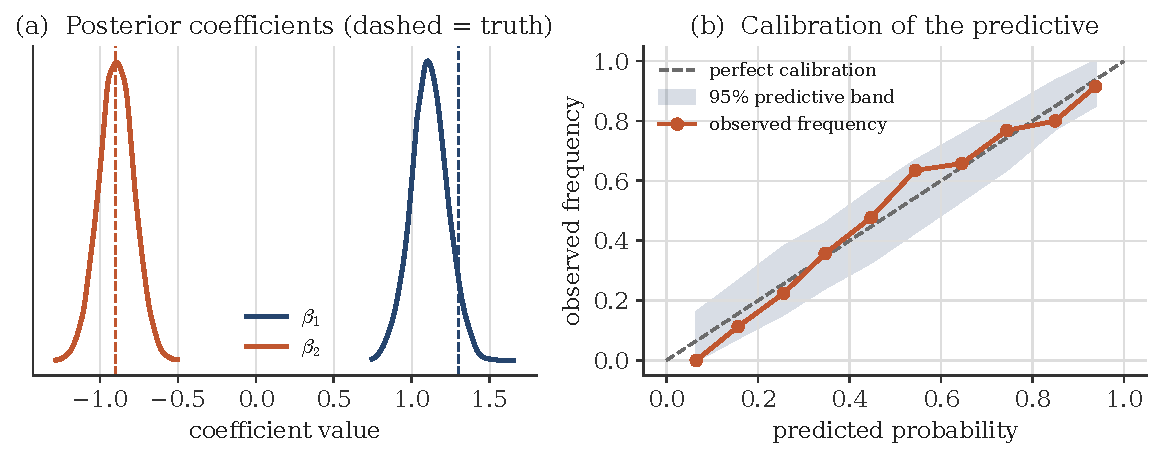
\includegraphics[width=0.9\textwidth]{app_logistic}
\caption{Bayesian logistic regression. (a) Posterior distributions of the coefficients, with
the data generating values dashed. (b) Calibration of the predictive: observed frequency against
predicted probability, with a $95\%$ band for binomial variation.}
\label{fig:app_logistic}
\end{figure}

\subsection{Dirichlet process mixtures: letting the data choose the model size}
How many clusters are in a data set is usually treated as a question to be answered before
modeling. The Dirichlet process mixture makes it part of the posterior. Given a sample drawn
from three overlapping populations, a collapsed Gibbs sampler over the DP mixture assigns
observations to clusters, creating new ones whenever the data demand them.
Figure~\ref{fig:app_dpm} shows the fitted predictive density against the histogram, with the
individual mixture components dashed beneath it. The sampler recovers the structure and prefers
a small number of components, splitting one broad mode into two rather than committing to a
single wrong shape. The number of clusters is not estimated and then fixed; it is integrated
over, which is the nonparametric predictive of Sections~\ref{ch:nonparametric} and~\ref{ch:bnp} at
work.\index{Dirichlet process}\index{mixture model}\index{nonparametric Bayes}

\begin{figure}[H]
\centering
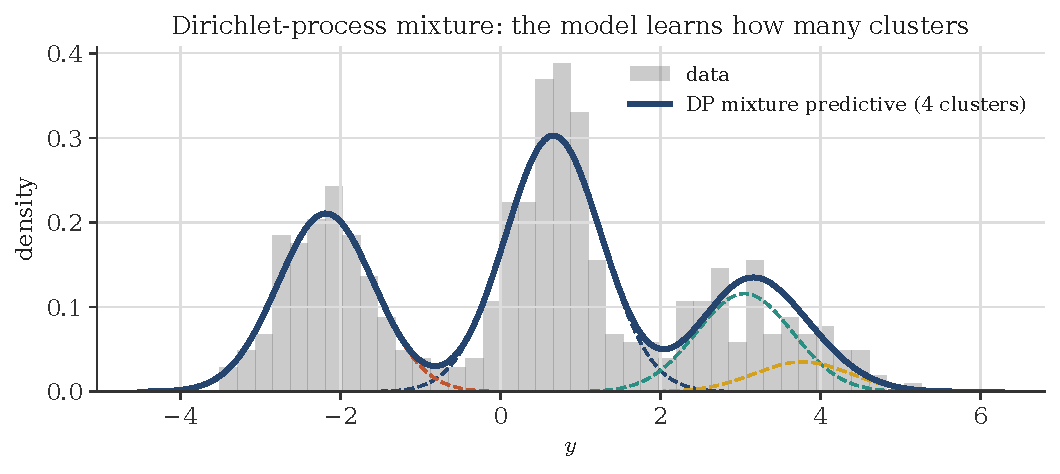
\includegraphics[width=0.9\textwidth]{app_dpm}
\caption{A Dirichlet process mixture fitted by collapsed Gibbs sampling. The predictive density
(solid) against the data, with the active mixture components dashed. The number of clusters is
a posterior quantity, not a tuning choice.}
\label{fig:app_dpm}
\end{figure}


\subsection{Meta analysis: combining evidence across studies}
Seven trials of the same treatment report log odds ratios of differing precision, and the
question is what the body of evidence says together. A random effects model treats the study
effects as exchangeable draws around a common mean, so each study is shrunk toward the
consensus in proportion to its own noise. Figure~\ref{fig:app_meta} places the raw study
estimates against their posteriors and marks the overall effect with its credible interval,
here about $0.37$ with a $95\%$ interval from $0.18$ to $0.61$. The small imprecise trials move
a long way toward the center while the large ones barely move, and the overall interval is
tighter than the raw interval of any single study. This is the eight schools calculation again, now in the setting
where it does the most public good.\index{meta analysis}\index{random effects}

\begin{figure}[H]
\centering
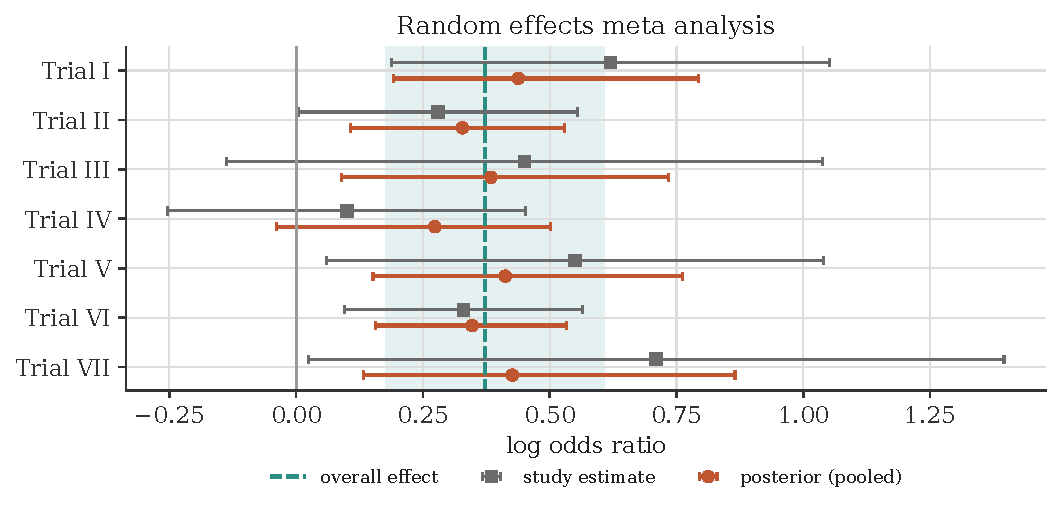
\includegraphics[width=0.9\textwidth]{app_meta}
\caption{Random effects meta analysis of seven trials. Study estimates with two standard error
bars, posterior intervals after pooling, and the overall effect with its credible band. Small
studies shrink most; the overall interval is tighter than any raw trial interval.}
\label{fig:app_meta}
\end{figure}

\subsection{Survival analysis with censored observations}
Clinical and reliability data arrive incomplete: some subjects are still alive when the study
ends, so their survival times are censored rather than observed. The likelihood handles this
without special pleading, contributing a density for a failure and a tail probability for a
censored case. Fitting a Weibull model to such data gives the posterior survival curve of
Figure~\ref{fig:app_survival}, plotted with its credible band against the empirical curve and
the truth. The band is narrow early, when many subjects remain at risk, and, relative to the curve, widens in the tail
where few observations survive to inform it. A point estimate of median survival would hide
that asymmetry of information.\index{survival analysis}\index{censoring}\index{Weibull model}

\begin{figure}[H]
\centering
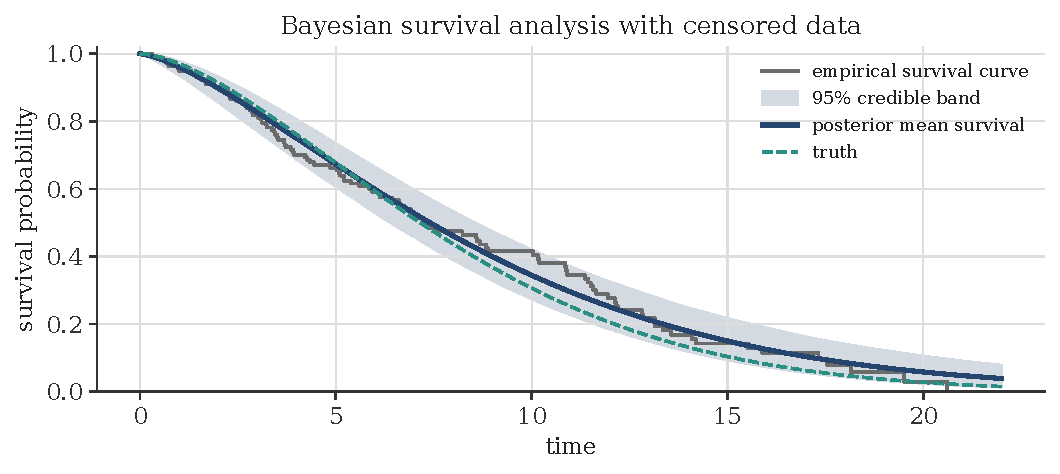
\includegraphics[width=0.9\textwidth]{app_survival}
\caption{Bayesian survival analysis under right censoring. Posterior mean survival curve with
its $95\%$ credible band, the empirical survival curve, and the data generating truth.
Relative uncertainty grows in the tail, where few subjects remain at risk.}
\label{fig:app_survival}
\end{figure}

\subsection{Spatial prediction: mapping a surface from scattered sites}
Forty five monitoring sites report a measurement at scattered locations, and a map is wanted
everywhere. A Gaussian process prior over the surface delivers one, but it also delivers the
second map that matters. Figure~\ref{fig:app_kriging}(a) shows the posterior mean surface, and
panel (b) the posterior standard deviation, which is small near the sites and grows in the
corners and gaps where no one has measured anything. Practitioners call this kriging; in the
language of this book it is the predictive distribution of a Gaussian random field, and
panel (b) is the honest statement of where the map should not be
trusted.\index{kriging}\index{spatial statistics}\index{random field}

\begin{figure}[H]
\centering
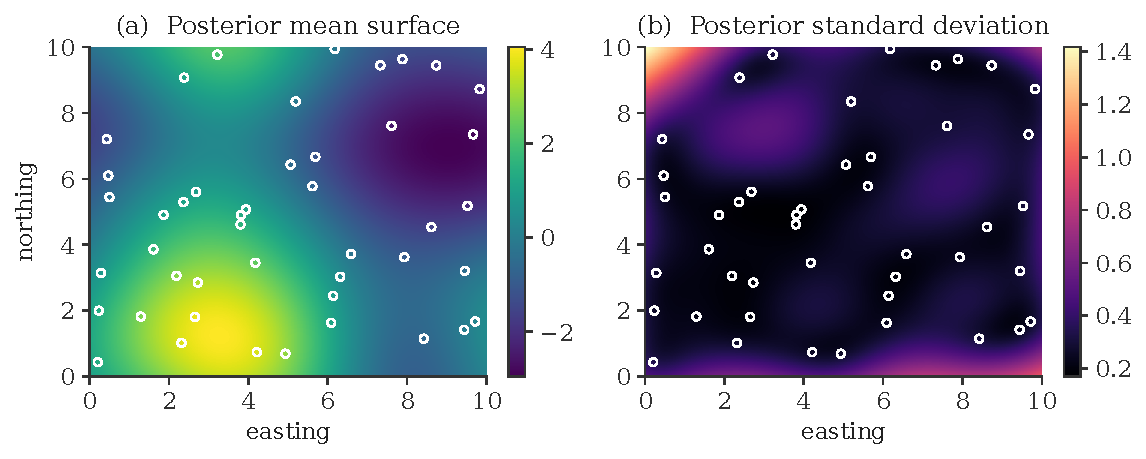
\includegraphics[width=0.9\textwidth]{app_kriging}
\caption{Spatial prediction from scattered sites (circles). (a) Posterior mean surface.
(b) Posterior standard deviation, small near the data and large in the unsampled corners. The
second panel is the part a contour map usually omits.}
\label{fig:app_kriging}
\end{figure}

\subsection{Epidemic nowcasting: estimating transmission as it changes}
During an outbreak the quantity that drives policy is the reproduction number $R_t$, the average
number of onward infections per case, and it must be estimated from noisy daily counts while it
is still moving. Placing a gamma prior on $R_t$ and updating it against the renewal equation
over a sliding window gives a posterior for every day, shown with its credible band in
Figure~\ref{fig:app_epidemic}. The estimate tracks the imposed decline and crosses one at close
to the right moment, and the width of the band is the answer to the question a policymaker
actually asks, namely how sure we are that transmission has fallen below the replacement
level.\index{epidemic model}\index{reproduction number}\index{nowcasting}

\begin{figure}[H]
\centering
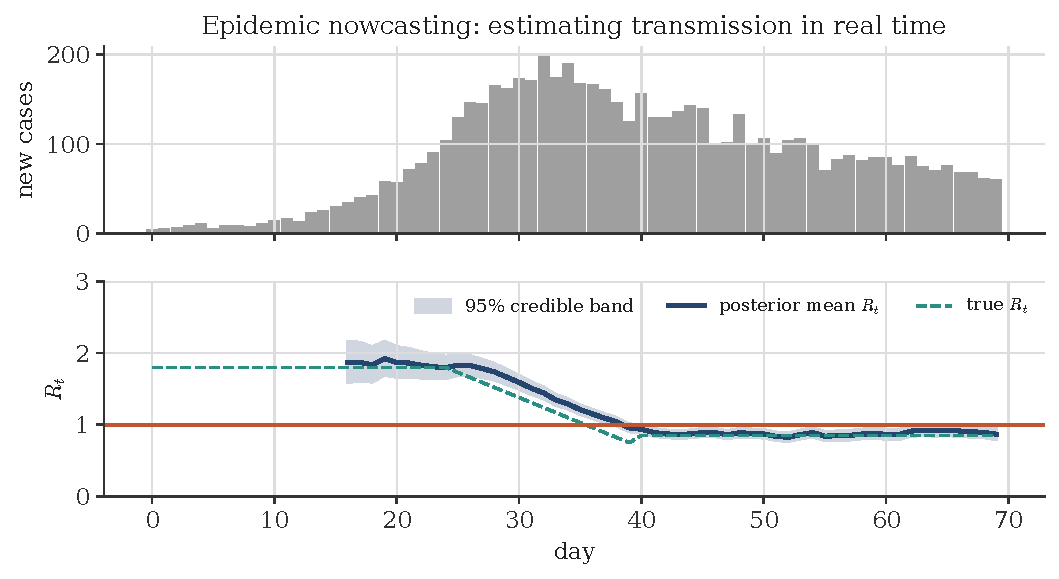
\includegraphics[width=0.9\textwidth]{app_epidemic}
\caption{Epidemic nowcasting. Top: observed daily cases. Bottom: posterior mean and $95\%$ band
for the reproduction number $R_t$ against the truth, with the critical value one marked. The
band, not the point estimate, answers the policy question.}
\label{fig:app_epidemic}
\end{figure}

\subsection{Item response theory: measuring ability from test answers}
Four hundred candidates answer six questions of differing difficulty and discrimination, and
the object of inference is each candidate's latent ability. The item response model supplies a
curve per question giving the probability of a correct answer as a function of ability, drawn
in Figure~\ref{fig:app_irt}(a); harder questions sit to the right and sharper ones rise more
steeply. Panel (b) compares posterior mean abilities against the values that generated the data,
with credible intervals on a subset. Recovery is good in the middle of the scale and visibly
noisier at the extremes, where six questions simply cannot pin down a candidate who answers
almost everything right or almost everything wrong. That is a property of the data, and the
posterior reports it rather than hiding it behind a
score.\index{item response theory}\index{latent variable model}\index{psychometrics}

\begin{figure}[H]
\centering
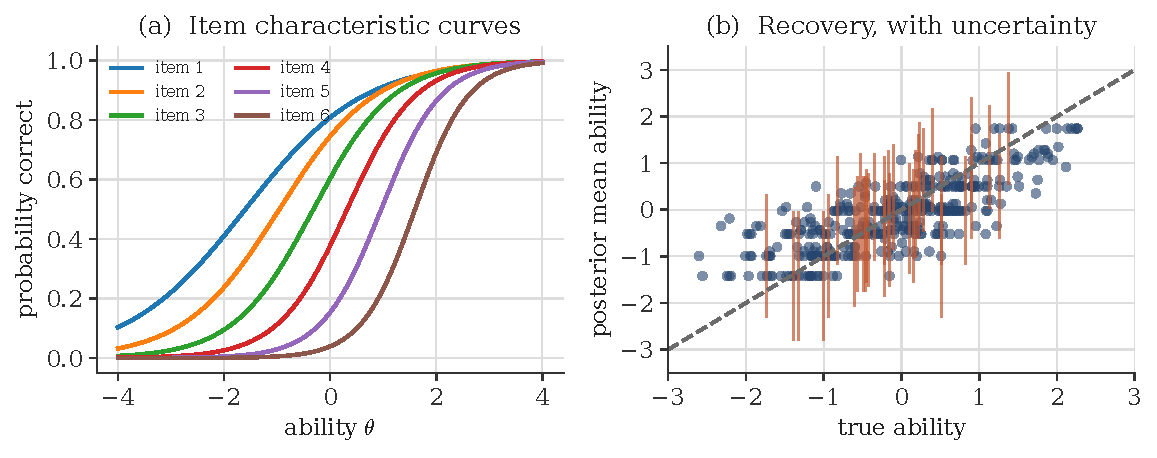
\includegraphics[width=0.9\textwidth]{app_irt}
\caption{Item response theory. (a) Item characteristic curves for six questions of differing
difficulty and discrimination. (b) Posterior mean ability against the truth with credible
intervals; precision degrades at the extremes of the scale, as it must.}
\label{fig:app_irt}
\end{figure}

\subsection{Bayesian optimization: choosing the next experiment}
An expensive function is to be maximized in as few evaluations as possible, which is the
situation in tuning a process, a drug dose, or a large model. The Bayesian answer keeps a
posterior over the function and uses it to score candidate points by expected improvement,
evaluating wherever that score is largest. Figure~\ref{fig:app_bayesopt} follows four steps: the
posterior band tightens where points have been taken, the acquisition score in gold shifts
between the promising region and the unexplored edges, and the procedure closes in on the
optimum while still occasionally probing far away. Exploration and exploitation are not balanced
by a tuning constant here; the balance falls out of the posterior
itself.\index{Bayesian optimization}\index{expected improvement}\index{active learning}

\begin{figure}[H]
\centering
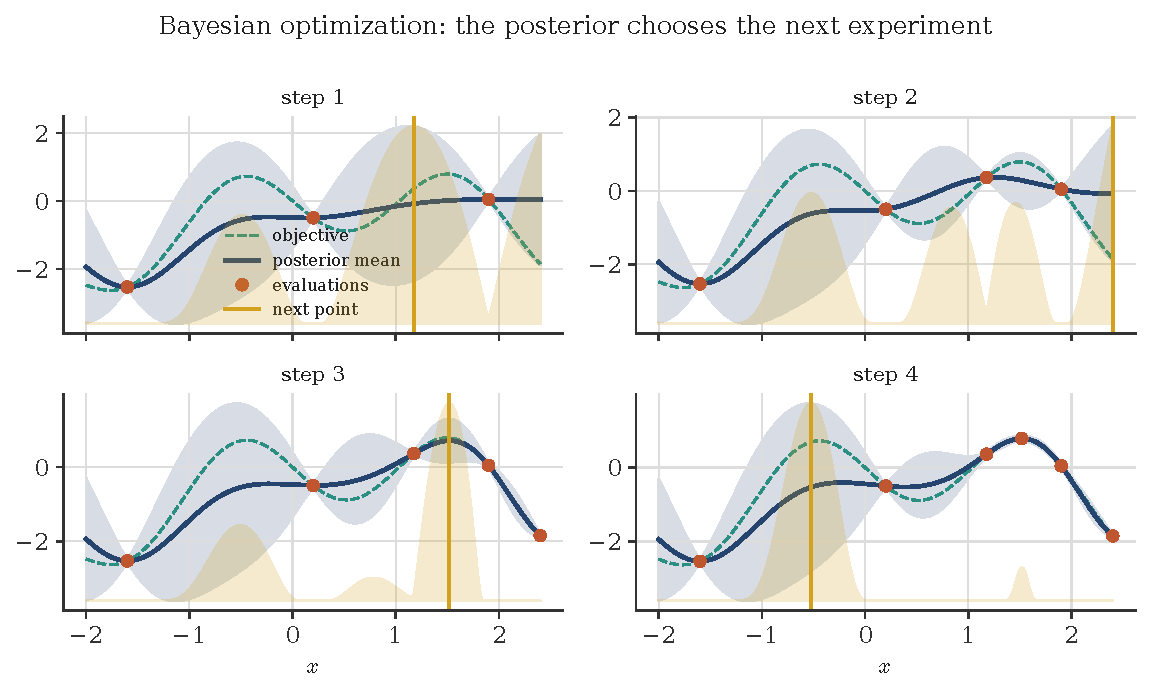
\includegraphics[width=0.9\textwidth]{app_bayesopt}
\caption{Bayesian optimization over four steps. Posterior mean and band for the objective, the
evaluations taken so far, the expected improvement score (shaded), and the point it selects
next. The posterior decides where to look, so exploration needs no separate tuning constant.}
\label{fig:app_bayesopt}
\end{figure}


\subsection{Multilevel regression with a group level predictor}
The eight schools model pools toward a single number. Real hierarchical work usually has more
structure: groups differ in ways that are themselves partly explained by something known about
the group. Here forty five groups of very unequal size each contribute a small regression, and a
group level covariate $u_j$ is available. The model gives every group its own intercept
$\alpha_j$ and regresses those intercepts on $u_j$, so a group with three observations is pulled
not toward the overall mean but toward the value its covariate predicts.
Figure~\ref{fig:app_multilevel}(a) shows how hard each group is pooled as a function of its
sample size, with the analytic weight $(\sigma^2/n_j)/(\sigma^2/n_j+\sigma_\alpha^2)$ drawn
through the fitted values: tiny groups are pooled hardest, large ones least,
and nothing has to be decided by hand. Panel (b) shows the group level regression doing the work,
recovering a slope of about $0.75$ against a true $0.72$. This is the everyday form of the
hierarchical idea, and the reason multilevel models dominate applied work in education,
epidemiology, and the social sciences.\index{multilevel model}\index{partial pooling}\index{varying intercepts}

\begin{figure}[H]
\centering
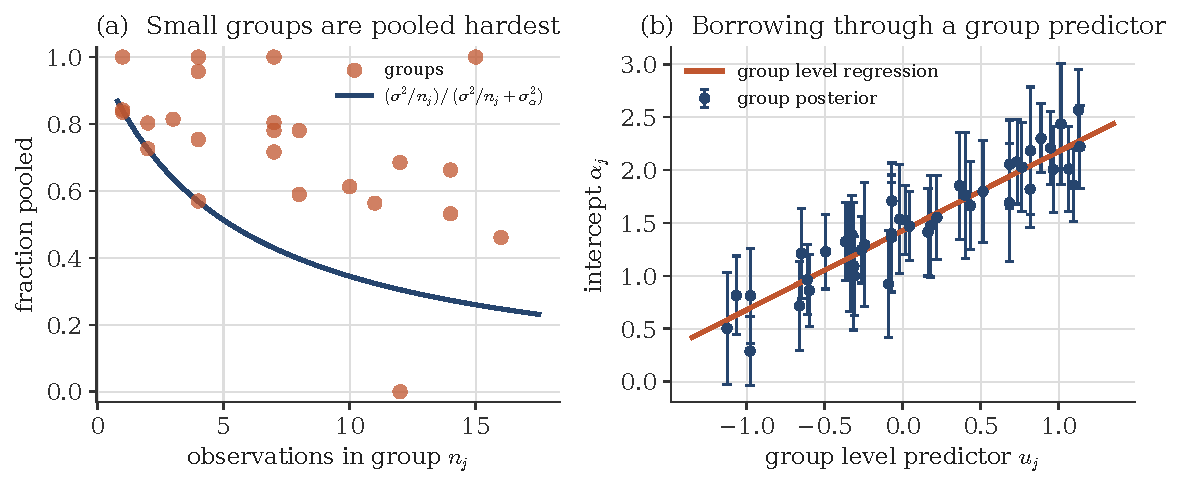
\includegraphics[width=0.9\textwidth]{app_multilevel}
\caption{Multilevel regression with a group level predictor. (a) The fraction of the way each
group is pooled, against its sample size, with the analytic shrinkage weight through it.
(b) Group intercepts with credible intervals against the group level covariate, and the fitted
group level regression that supplies each group's prior mean.}
\label{fig:app_multilevel}
\end{figure}

\subsection{Growth curves: random intercepts and random slopes}
Longitudinal data give each subject a trajectory, and the interesting question is rarely the
average path alone but how much subjects differ in where they start and in how fast they change.
Letting both the intercept and the slope vary by subject, with a joint prior across the pair,
gives the fit in Figure~\ref{fig:app_growth}(a): twenty individual curves drawn from their
posteriors, with the population mean curve through them. Panel (b) separates the two sources of
uncertainty that a single regression line would confound, showing the spread of individual
slopes against the much tighter posterior for the population slope. The distinction matters in
practice: a treatment can raise the average trajectory while leaving individual variation
untouched, and only the hierarchical fit can say which has
happened.\index{growth curve}\index{random slopes}\index{longitudinal data}

\begin{figure}[H]
\centering
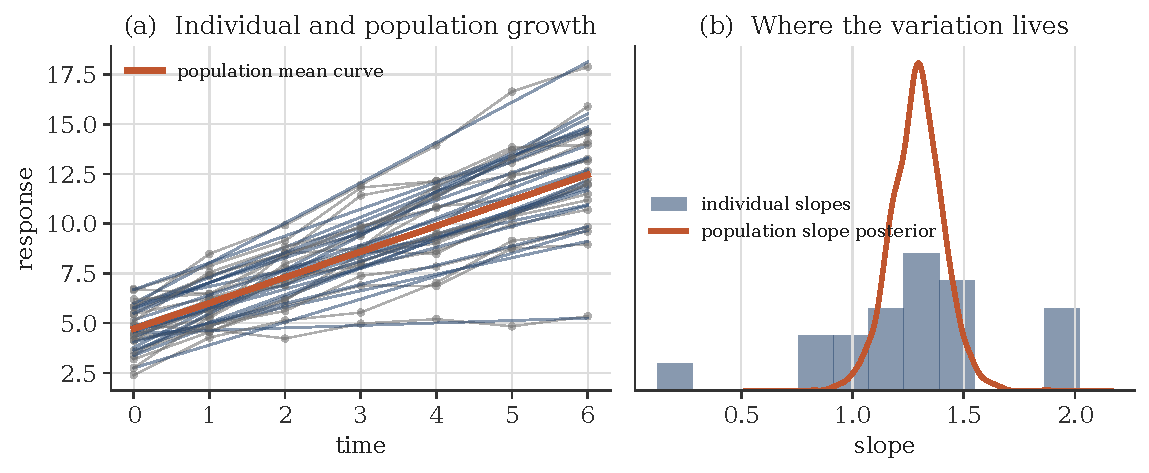
\includegraphics[width=0.9\textwidth]{app_growth}
\caption{Hierarchical growth curves. (a) Observed trajectories with posterior individual curves
and the population mean curve. (b) The spread of individual slopes against the posterior for the
population slope; the two answer different questions and the hierarchy keeps them apart.}
\label{fig:app_growth}
\end{figure}

\subsection{Small area estimation: mapping risk from sparse counts}
Disease mapping is where naive ratios fail most visibly. Each of one hundred and forty four
areas reports an observed count against an expected count, and the raw ratio $O_i/E_i$ is
violently unstable wherever the expected count is small, so the extreme areas on a raw map can be
the ones with the least data. A hierarchical Poisson model with an area level random
effect fixes this by pooling each area toward the overall level in inverse proportion to its own precision. Figure~\ref{fig:app_smallarea} shows the raw map, the posterior mean risk map, and
the expected counts that explain the difference. The smoothed map has a standard deviation of
$0.38$ against $0.58$ for the raw one, and the areas that lose the most are the sparse
ones in panel (c). This is shrinkage as public health practice, and it is the same calculation
as the eight schools, applied one hundred and forty four
times.\index{small area estimation}\index{disease mapping}\index{hierarchical Poisson model}

\begin{figure}[H]
\centering
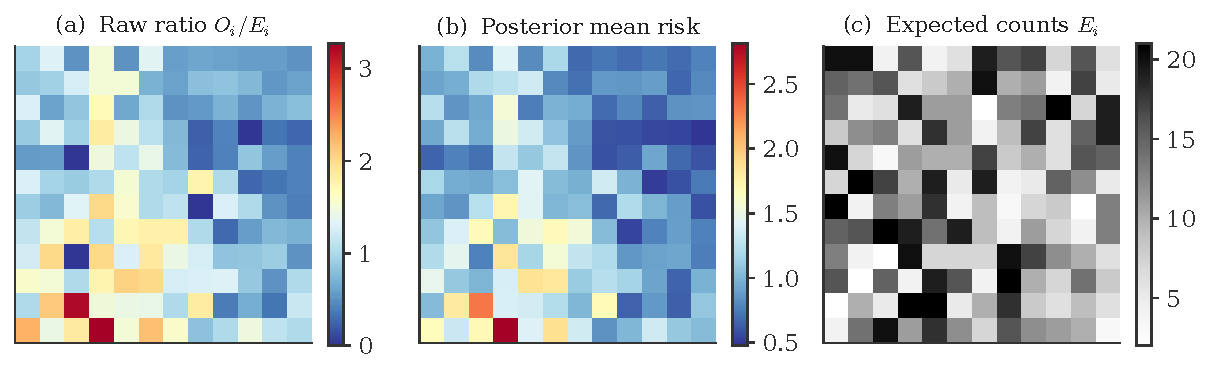
\includegraphics[width=0.9\textwidth]{app_smallarea}
\caption{Small area estimation. (a) Raw standardized ratios, unstable where data are thin.
(b) Posterior mean risk under a hierarchical Poisson model. (c) Expected counts, which set how
far each area is pooled. Some extreme values in (a) sit where (c) is smallest.}
\label{fig:app_smallarea}
\end{figure}

\paragraph{Summary.}
Every vignette returns a posterior and reads its answer from it: a shipping decision from an expected loss, an uncertainty band that is narrow near the data and wide where information is scarce (Gaussian process and kriging, and survival relative to the curve), and a pooling weight that borrows strength across groups and pools small noisy ones hardest (hierarchical shrinkage, meta analysis, multilevel regression, and small area estimation). In the bandit and Bayesian optimization vignettes the posterior is the policy, in the change point and Dirichlet process vignettes it is a distribution over where the break occurs and how many clusters there are, and the posterior predictive check, the funnel, the MCMC diagnostics, and calibration audit the model and the sampler.

\subsection*{Problems}
\begin{enumerate}[leftmargin=1.8em,itemsep=2pt]
\item In the A/B test, replace the symmetric loss by one that charges three times as much for a wrongful switch as for a missed gain, and recompute the decision from the posterior of the uplift.
\item Derive the posterior for the between group standard deviation $\tau$ in the eight schools model with flat priors on $\mu$ and $\tau$, and explain why its mass near zero drives the pooling.
\item Write the noncentered parametrization $\theta_j=\mu+\tau\eta_j$ and show that the prior on $(\eta_j,\tau)$ has no funnel, while the prior on $(\theta_j,\tau)$ does.
\item For the posterior predictive check, propose a discrepancy that a Poisson model can fake and one it cannot, and explain the difference in terms of the sufficient statistic.
\item Show that the Kalman gain is the posterior weight on the new observation in a conjugate normal update, and that the filtered variance never exceeds the predicted variance.
\item In the small area model, show that the posterior mean risk for an area is pulled toward the overall level by an amount that decreases in its expected count, and identify the limit as the count grows.
\item Implement the collapsed Gibbs sampler for the Dirichlet process mixture and report how the number of occupied clusters behaves as the concentration parameter is varied.
\end{enumerate}

\section{Worked Examples and the Thermodynamic Reading}\label{ch:examples}

\noindent\textbf{Thesis.} The constrained-horizon construction is best understood
through statistical mechanics and through four examples worked to the end. The
conditioned ensemble is microcanonical relative to the reference law; the product
$I$-projection is its canonical local equilibrium; and the split radius
$\delta_N\asymp\sqrt{(k\log N)/N}$ is where the entropy of the type lattice
balances the divergence barrier. The examples then exhibit every branch of the
reachability dichotomy of Section~\ref{ch:projected}: a degenerate affine
constraint where no prior survives, a prior-null constraint where the co-area
conditional beats the naive $\sigma$-reweighting, the Brandeis dice as the
unreachable maximum-entropy tilt, and Gaussian scale mixtures as the continuous
analogue.

\subsection{Thermodynamic reading and local fluctuations}
\label{sec:thermo}

The language of statistical mechanics is useful here, provided the reference
law $\mu$ is kept visible.

\emph{Microcanonical horizon.} Conditioning on
$\{\widehat{P}_N\in E_{\varepsilon_N}\}$ discards configurations whose empirical
moments fall outside the prescribed window. The remaining configurations retain
their weights under $\mu^{\otimes N}$; they are equiprobable only for a uniform
baseline. Thus the ensemble is microcanonical, or approximately so, relative to
$\mu$. The restriction belongs to the horizon as a whole, not to any one
coordinate.

\emph{Canonical local equilibrium.} The product $I$-projection
$(\Pstar_\mu)^{\otimes m}$ supplies the corresponding canonical law. Its Lagrange
multipliers tilt the baseline just enough to reproduce the prescribed moments.
Theorem~\ref{thm:master} makes the local equivalence precise: a fixed block from
the globally constrained horizon is close to independent draws from
$\Pstar_\mu$, with an explicit finite-$N$ error that does not depend on where the
block is located.

\emph{Free energy.} By the method of types
$\Pb_\mu(\widehat{P}_N=Q)=a_N(Q)\,e^{-N\D{Q}{\mu}}$ with $(N+1)^{-k}\le a_N(Q)\le1$,
and
\begin{equation}
\label{eq:freeenergy}
\D{Q}{\mu}=-H(Q)-\sum_x Q(x)\log\mu(x).
\end{equation}
The summation term in \eqref{eq:freeenergy} is the energy relative to the
baseline, while $H(Q)$ is the entropy. Their difference $\D{Q}{\mu}$ is the
intensive free-energy cost of the macrostate $Q$.
Minimizing that cost over the admissible set gives the $I$-projection
$\Pstar_\mu$.

\emph{Entropy-energy balance.} The bad-type mass in the proof obeys
$\beta_N(\delta)\le C(\mu,E)\exp\{2k\log(N+1)-2N\delta^2\}$. The logarithmic term
accounts for the at most $(N+1)^k$ types and the corresponding normalization of the
conditioning denominator; the extensive term $2N\delta^2$ is the
relative-entropy barrier.
Balancing them gives $N\delta_N^2\asymp k\log N$, hence
$\delta_N\asymp\sqrt{(k\log N)/N}$, the tuning of
Corollary~\ref{cor:tuning}. This split radius, distinct from the window radius
$\varepsilon_N$, is where the combinatorial entropy of the type lattice is balanced
by the divergence cost of leaving the projection.

\emph{Relation to PAC-Bayes.} The same architecture governs Gibbs-posterior and
PAC-Bayesian concentration (Catoni, 2007). PAC-Bayes bounds the excess risk of a
randomized predictor at a square-root complexity-to-sample-size scale, with
complexity measured by relative entropy between posterior and prior.
Corollary~\ref{cor:tuning} has the analogous scale
$\sqrt{(k\log N)/N}$: the logarithmic complexity of the type lattice is divided by
the horizon, while excess relative entropy from the constrained equilibrium
provides the barrier. Moreover, both the Gibbs posterior of PAC-Bayes and the
conditional type law $w_N$ in the split-set weights (Section~\ref{ch:master}) are exponential tilts of a
reference measure by an empirical cost. The correspondence is structural, not a
claim of a generalization bound: here the state space consists of empirical types,
the cost is excess relative entropy from canonical equilibrium, and the conclusion
is a local equivalence of ensembles.

\subsubsection{Local fluctuations on the
\texorpdfstring{$N^{-1/2}$}{inverse-square-root N} scale}
\label{sec:fluctuations}

The master inequality is a global concentration statement, controlling the
probability of leaving a fixed or slowly shrinking neighborhood of $\Pstar$. Inside
that neighborhood, on the $N^{-1/2}$ scale, there is a complementary local
refinement, which we record for the regular affine case; the global
Gibbs-conditioning theorem does not by itself supply it.

\begin{remark}[Local Gaussian fluctuations; companion paper]
\label{rem:fluct}
Under exact feasibility on the type lattice and an affine local slice with
no active inequality, the conditional law of $\sqrt N(\widehat{P}_N-\Pstar)$ is
asymptotically Gaussian on the constraint tangent space, with precision the reduced
Hessian of $\D{\cdot}{\mu}$ at $\Pstar$. Consequently
$2N\,\D{\widehat{P}_N}{\Pstar}$ is asymptotically chi-square with $k-1-r_0$ degrees of
freedom, the limit of Remark~\ref{rem:cbvm}, which checks it by simulation for the Brandeis die. Here $r_0$ is the number of equality constraints; no inequality is active
on the slice, whereas $r$ counts constraints of both kinds.
\end{remark}

Neither the master inequality nor a shrinking window supplies this refinement. Any
admissible window satisfies $N\varepsilon_N>c_{\mathrm{rnd}}$ and is therefore thicker
than the $O(1/N)$ mesh of the type lattice, so the feasible types acquire a normal
component and a two-scale local limit theorem would be required, resolving $N^{-1/2}$
tangential fluctuations together with a normal scale determined jointly by the shrinking
window and the $O(1/N)$ lattice mesh. Exact feasibility collapses the feasible set
onto a single tangent slice, which is what makes the single-scale Gaussian available.
The companion paper (Polson and Zantedeschi, 2025b; Section~\ref{ch:moment}) develops the exact-feasibility
Gaussian theorem, its chart geometry, and the associated estimation theory, while
leaving the thickened case open. Thus Theorem~\ref{thm:master} and
Remark~\ref{rem:fluct} are complementary: the former gives global concentration
under a window, the latter local geometry without one.

Two distinct local Gaussian phenomena appear, in opposite arguments of the
divergence. Forward conditional Sanov gives Gaussian fluctuations of the empirical
type around the $I$-projection on the constraint tangent space
(Remark~\ref{rem:fluct}). Inverse Sanov gives Gaussian posterior fluctuations of
the directing law around the empirical distribution: for a true interior component
$\mu_0$ and a prior density positive and continuous at $\mu_0$, the ordinary
finite-dimensional Bernstein--von Mises theorem (van der Vaart, 1998, Theorem~10.1) gives, in any
smooth $(k-1)$-dimensional chart,
\[
\mathcal{L}\big(\sqrt N(\mu-\widehat{P}_N)\mid X_{1:N}\big)\ \toL\
\N_{k-1}\big(0,\mathcal{I}(\mu_0)^{-1}\big),
\]
the ambient covariance being
$\operatorname{diag}(\mu_0)-\mu_0\mu_0^\top$ restricted to the simplex tangent
space. Both arise from the local quadratic expansion of relative entropy, in
opposite arguments: the empirical type fluctuates around the projected law, and the
posterior directing law fluctuates around the empirical type.

\subsection{Examples}
\label{sec:examples}

\subsubsection{Bernoulli components}
\label{sec:bernoulli}

The simplest case: with $\mu=\mathrm{Ber}(0.2)$ and the horizon
mean constrained near $0.8$, every fixed target inside the horizon is
asymptotically $\mathrm{Ber}(0.8)$, the $I$-projection, regardless of its temporal label.

The binary case is small enough to evaluate exactly. Conditionally on a type the
block is hypergeometric, so the Heath--Sudderth mixture (Section~\ref{ch:types}) gives the constrained block law in closed
form and its distance to $(\Pstar)^{\otimes m}$ needs no simulation.
Table~\ref{tab:bern} separates the two contributions of
Theorem~\ref{thm:master} for $m=5$ and $\varepsilon_N=N^{-1/2}$: the split-set term,
which collects the type concentration and the finite-population coupling, and the
window-transfer term $\lVert (P^\bullet)^{\otimes m}-(\Pstar)^{\otimes m}\rVert_{\mathrm{TV}}$.

\begin{table}[t]
\centering
\footnotesize
\caption{Exact total variation for the constrained block law. $\mu=\mathrm{Ber}(0.2)$,
horizon mean $0.8$, $m=5$, $\varepsilon_N=N^{-1/2}$. All three entries are exact
distances: split-set is $\lVert L_{N,I_N,\mu}-(P^\bullet)^{\otimes m}\rVert_{\mathrm{TV}}$, window is
$\lVert (P^\bullet)^{\otimes m}-(\Pstar)^{\otimes m}\rVert_{\mathrm{TV}}$, total is
$\lVert L_{N,I_N,\mu}-(\Pstar)^{\otimes m}\rVert_{\mathrm{TV}}$. They are related by the triangle
inequality, not by addition; the window term is the binding contribution.}
\label{tab:bern}
\begin{tabular}{@{}r@{\ \ }c@{\ \ }c@{\ \ }c@{\ \ }c@{}}
\hline
$N$ & $\varepsilon_N$ & split-set & window & total \\
\hline
$25$ & $0.200$ & $0.045$ & $0.400$ & $0.410$ \\
$100$ & $0.100$ & $0.013$ & $0.209$ & $0.209$ \\
$400$ & $0.050$ & $0.003$ & $0.104$ & $0.104$ \\
$800$ & $0.035$ & $0.001$ & $0.074$ & $0.073$ \\
$1600$ & $0.025$ & $0.001$ & $0.052$ & $0.052$ \\
\hline
\end{tabular}
\end{table}

At every horizon the split-set term is smaller than its coupling budget
$m(m-1)/(2N)$ by a factor between six and twelve: it is $0.045$ against $0.400$
at $N=25$, and $0.003$ against $0.025$ at $N=400$. The window width is therefore
the binding contribution.

The equality constraint here is affine with $r_0=1$ on an alphabet of size $k=2$, so
$k-1-r_0=0$ and Proposition~\ref{prop:reach}(iv) forces the projected directing
measure to be degenerate: $E$ is the singleton $\{\mathrm{Ber}(0.8)\}$ and $\Pstar_\mu=\mathrm{Ber}(0.8)$
for every $\mu$. Numerically, at $N=800$ with $m=2$, the constrained block law agrees to within
$0.005$ in total variation across the baselines $\mathrm{Ber}(0.05)$, $\mathrm{Ber}(0.2)$, $\mathrm{Ber}(0.5)$,
and $\mathrm{Ber}(0.7)$, each sitting within $0.056$ of $\mathrm{Ber}(0.8)^{\otimes m}$: no prior
survives.

The inequality constraint $E=\{Q:Q(1)\ge\alpha\}$ is a different branch, and clause
(iv) does not apply to it: $E$ is not affine, and $T_E$ is the identity on
$\{\mu\ge\alpha\}$ and constant on $\{\mu<\alpha\}$, so it is neither an orbit quotient
nor injective. It is instead the reachable branch with positive prior mass, and
clause (i) of Proposition~\ref{prop:reach} applies to it directly: $\Pi(\partial E)=\Pi(\{\alpha\})=0$
in $\Delta(\X)$ for any prior without an atom at $\alpha$, so the boundary condition of that clause holds. With
$\Pi=\mathrm{Beta}(2,2)$ and $\alpha=0.6$ the set $E$ carries $35.2\%$ of the prior, so
$\Pi_E=\Pi(\cdot\mid\mu\ge\alpha)$, with $\E[\mu\mid\mu\ge\alpha]=0.745$ and standard
deviation $0.097$; the finite-horizon posterior means, under the window $\varepsilon_N=N^{-1/2}$, rise to it, from $0.619$ at $N=25$
to $0.735$ at $N=3200$. The directing measure is random. On
$\{\mu\ge\alpha\}$, however, the projection is the identity, so the limiting randomness
is the truncated prior, while the componentwise tilt contributes only at finite
$N$ through the bound of Theorem~\ref{thm:master}.

\subsubsection{A null constraint set: the co-area conditional}
\label{sec:trap}

For a regular prior and a prior-null equality constraint,
Proposition~\ref{prop:reach}(ii) gives the relevant limit; in this setting the
constraint large-deviation rate $I_E$ (Section~\ref{ch:projected}) does not by itself identify the
conditional.
Specifically, take $\X=\{1,2,3\}$, $g(x)=x$, the single equality constraint
$E=\{Q:\E_Q[X]=\alpha\}$ with $\alpha=2.2$, and the flat prior
$\Pi=\mathrm{Dir}(1,1,1)$. Then $\Pi(E)=0$, because $E$ is a segment in the
simplex, while $I_E$ vanishes on $E$. Proposition~\ref{prop:reach}(ii)
applies, since $\operatorname{supp}\Pi$ is the whole simplex, and the disintegration it names is well defined: the pushforward of $\Pi$ under
$\mu\mapsto\E_\mu[X]$ has a continuous positive density at $\alpha=2.2$.

The segment is $\mu(u)=(u-0.2,\,1.2-2u,\,u)$ for $u\in[0.2,0.6]$, with
$\sigma^2(\mu(u))=\operatorname{Var}_\mu(X)=2u-0.24$, running from $0.16$ at the die
$(0,0.8,0.2)$ to $0.96$ at the die $(0.4,0,0.6)$. The constraint map is affine and the
prior is flat, so the co-area disintegration is uniform in $u$ and predicts
$\E[\mu_3\mid E]=0.4$ exactly. Laplace's method applied to the constraint large-deviation rate $I_E$ (Section~\ref{ch:projected})
alone predicts instead the $\sigma$-reweighted law $\Pi_E\propto\sigma(\mu)\,\Pi$, giving
$0.4255$. The two differ by $2.6$ percentage points in a predictive probability, since
$\mu_3$ is the limiting $\Pb(X_{t+1}=3)$.

The finite-$N$ constraint posterior settles it. The type law is trinomial, so
$\Pb_\mu(E_N)$ is a finite sum and $\Pi_{N,E}$ can be evaluated exactly, without
simulation, under either the window $E_{\varepsilon_N}$ or exact conditioning on
$\{\bar X_N=2.2\}$. Table~\ref{tab:trap} reports it.

\begin{table}[htbp]
\centering
\footnotesize
\caption{$\E[\mu_3\mid E_N]$ under the exact constraint posterior.
$\X=\{1,2,3\}$, $\E_Q[X]=2.2$, $\Pi=\mathrm{Dir}(1,1,1)$. Co-area predicts
$0.400$; the $\sigma$-reweighted law predicts $0.4255$.}
\label{tab:trap}
\begin{tabular}{@{}r@{\quad}c@{\quad}c@{}}
\hline
$N$ & window, $\varepsilon_N=N^{-1/2}$ & exact, $\{\bar X_N=2.2\}$ \\
\hline
$100$ & $0.394$ & $0.398$ \\
$400$ & $0.398$ & $0.400$ \\
$1600$ & $0.400$ & $0.400$ \\
\hline
\end{tabular}
\end{table}

Both schemes converge to $0.400$ from below at rate $O(1/N)$, and the
$\sigma$-reweighting is excluded. The reason is the cancellation behind
Proposition~\ref{prop:reach}(ii), noted in the null-constraint example of Section~\ref{ch:projected}: the polynomial prefactor omitted by
the constraint large-deviation rate $I_E$ (Section~\ref{ch:projected}) carries $\det\Omega^{-1/2}$ (with $\Omega=\sigma^2(\mu)$ the covariance of the constraint statistic), which cancels the
Jacobian $\det\Omega^{1/2}$ contributed by the Gaussian tube. A large-deviation rate
identifies where the posterior concentrates; it does not by itself identify the
conditional it concentrates to.

\subsubsection{The Brandeis dice problem}
\label{sec:dice}

For each active horizon $N$, impose the empirical-average constraint
$\sum_{i=1}^{6} i\,\Phat_N(i)\approx 4.5$, against the fair value $3.5$. The baseline is
uniform, so the $I$-projection is a maximum-entropy tilt,
\[
p_i=\frac{e^{\lambda i}}{\sum_{j=1}^6 e^{\lambda j}},\qquad \lambda\approx0.37105,
\]
giving $p\approx(0.054,0.079,0.114,0.165,0.240,0.347)$ with
$H\approx1.614<\log6$. See Jaynes (1963) for the dice problem, Jaynes (1957) for the maximum-entropy analysis, and
Seidenfeld (1987) for a critical discussion of its Bayesian predictive
interpretation. Any fixed finite collection of
throws in that horizon has a local law converging to the product of this tilt,
including throws labeled future relative to any finite cut; when the baseline die
is fixed and uniform, the limiting constrained process is i.i.d.\ from the Jaynes
tilt. The uniform die has mean $3.5\neq4.5$, so $I^\star>0$: this is the unreachable
branch of Proposition~\ref{prop:reach}(iii), with a point-mass prior, hence
degenerate (Proposition~\ref{prop:reach}). Under uncertain die laws, $\widetilde{\Pi}_E=(\mu\mapsto\Pstar_\mu)_\#\Pi_E$ is the induced
prior over constrained die laws and sequential prediction is the Bayesian mixture.

\subsubsection{Gaussian scale mixtures}
\label{sec:gaussian}

Under the usual exponential-integrability and regularity conditions, the continuous
Gibbs conditioning principle extends the same structure beyond finite alphabets
(L\'eonard and Najim, 2002). We use Gaussian scale mixtures as an illustration.

The Gaussian components arise from symmetry rather than assumption.
Kingman (1972) shows that if every finite sample from an infinite sequence has a
spherically symmetric joint law, then conditionally on a single random variable $V$
the coordinates are i.i.d.\ $\N(0,V)$. The argument is a characteristic-function one:
spherical symmetry forces the characteristic function of a finite block to depend on
$t$ only through $\lVert t\rVert$; Schoenberg's theorem (Schoenberg, 1938)
identifies the admissible radial forms as Gaussian scale mixtures, with mixing
variable $V$.
Smith (1981) gives the centered variant, with a random mean as well, and
Ressel (1985) gives an analytic account. The result is the natural continuous
counterpart of the scalar-type construction in Section~\ref{ch:types}: compactness of
$[0,1]$ and Helly selection produce the mixing law there, whereas spherical
symmetry and Schoenberg's theorem produce it here. In particular, the theorem
supplies the prior over Gaussian directing components on which the constraint acts.

Although Proposition~\ref{prop:reach} is stated for a finite alphabet, the same
interpretation applies. Suppose the prior over $(M,V)$
charges every neighborhood of a component with the prescribed moments, so that
$E\cap\operatorname{supp}\Pi\neq\varnothing$ and $I^\star=0$. Reachability is
relative to $\operatorname{supp}\Pi$; the mere existence of a Gaussian with the
prescribed moments is not enough. Then $T_E$ is the identity on $E$, and the
surviving heterogeneity depends on how the constraint reweights the prior. Under
mean-only conditioning, the $I$-projection of $\N(M,V)$ is $\N(\theta,V)$, which
retains the variance. The limit therefore mixes $\N(\theta,V)$ over a conditional
law of $V$ and is nondegenerate exactly when that conditional law is.

The form of the conditional law depends on the regime. If $\Pi$ has a regular
density in $(M,V)$, the
constraint is $\Pi$-null and the same normal-direction cancellation as in
the null-constraint example of Section~\ref{ch:projected} applies: for fixed $V$,
\begin{equation}
\label{eq:gaussfubini}
\int_{\R}\Pb_{M,V}\big(|\bar X_N-\theta|\le\varepsilon_N\big)\,dM=2\varepsilon_N
\end{equation}
for every $V$, so the limit is the co-area conditional at $M=\theta$ carrying \emph{no}
additional variance factor. A larger $V$ does lower acceptance at the exact component
$M=\theta$, but it widens the range of nearby $M$ that can produce the event, and the
two effects cancel exactly. This is a continuous analogue of
Proposition~\ref{prop:reach}(ii), not an application of it, because the proposition is stated
for finite alphabets. If instead $\Pi$ places positive mass on $\{M=\theta\}$, the
constraint is not $\Pi$-null, \eqref{eq:gaussfubini} does not apply, and a window of
order $N^{-1/2}$ reweights those atoms through their componentwise acceptance
probabilities, as in Section~\ref{ch:projected}. Under mean-and-variance conditioning, the projection is
$\N(\theta,v)$ for every component; both parameters are pinned, and the mixture
collapses to the single product law $\N(\theta,v)^{\otimes m}$. A finite-block
continuous theorem with rates in the present mixture-level, shrinking-window
generality remains open.


\paragraph{Summary.}
The worked examples read the constrained horizon as a statistical mechanics problem: the conditioned ensemble is microcanonical relative to the reference law, the product $I$-projection is its canonical local equilibrium, and the split radius $\delta_N\asymp\sqrt{(k\log N)/N}$ balances the entropy of the type lattice against the divergence barrier. Four examples exhibit the branches of the reachability dichotomy: Bernoulli components, where an affine constraint with $k-1-r_0=0$ leaves no prior and an inequality constraint truncates the prior; the null-constraint trap, whose exact constraint posterior converges to $0.400$ and excludes the $\sigma$-reweighted $0.4255$; the Brandeis dice, an unreachable maximum-entropy tilt with $\lambda\approx0.371$; and Gaussian scale mixtures, the continuous analogue, where mean-only conditioning keeps the variance and mean-and-variance conditioning collapses the mixture.

\subsection*{Problems}
\begin{enumerate}[leftmargin=2.2em,itemsep=2pt]
\item Verify \eqref{eq:freeenergy} from the definition of $\D{Q}{\mu}$, and show that for the uniform baseline on $\{1,\dots,6\}$ the minimizer of $\D{Q}{\mu}$ under $\sum_{i=1}^{6} i\,Q(i)=4.5$ has the form $p_i\propto e^{\lambda i}$.
\item Solve $\sum_{i=1}^{6} i\,p_i=4.5$ for $\lambda$ in the dice tilt, and confirm $\lambda\approx0.37105$, the listed probabilities $p$, and $H\approx1.614<\log6$.
\item Reproduce the window column of Table~\ref{tab:bern} at $N=25$ and $N=100$. Show that the window projection of $\mathrm{Ber}(0.2)$ onto $E_{\varepsilon_N}=\{Q:\lvert Q(1)-0.8\rvert\le\varepsilon_N\}$ is $P^\bullet=\mathrm{Ber}(0.8-\varepsilon_N)$, and evaluate $\lVert(P^\bullet)^{\otimes5}-\mathrm{Ber}(0.8)^{\otimes5}\rVert_{\mathrm{TV}}$ as a sum over the number of ones.
\item On the segment $\mu(u)=(u-0.2,\,1.2-2u,\,u)$ of the null-constraint trap, show that $\E_\mu[X]=2.2$ and $\operatorname{Var}_\mu(X)=2u-0.24$. Compute $\E[\mu_3]$ when $u$ is uniform on $[0.2,0.6]$ and when its density is proportional to $\sigma(\mu(u))$, confirm $0.400$ and $0.4255$, and say which value Table~\ref{tab:trap} supports.
\item Prove \eqref{eq:gaussfubini} by Fubini's theorem, and show that the $I$-projection of $\N(M,V)$ onto $\{Q:\E_Q[X]=\theta\}$ is $\N(\theta,V)$.
\item Use Remark~\ref{rem:fluct}, under exact conditioning on the constraint, to give the limit law of $2N\,\D{\Phat_N}{\Pstar}$ for the Brandeis dice ($k=6$, one equality constraint) and for the binary example of Table~\ref{tab:bern}, and explain why the second is degenerate.
\end{enumerate}

\src{De Finetti + Sanov = Bayes (2509.13283), \S7--8 (thermodynamic reading, worked examples); companion Bayesian Prediction under Moment Conditioning (2510.20742).}

%=====================================================================
% CHAPTER: Federated Learning, de Finetti, and Sanov
% Chapter for "Elements of Bayes and Information Theory"
% Assumes: amsmath, amsthm, amssymb; theorem environments named
% theorem/proposition/corollary/definition/remark/algorithm
%=====================================================================

\section{Federated Learning, de Finetti, and Sanov}\label{ch:federated}

\noindent\textbf{Thesis.} De Finetti makes the federated model well-posed: exchangeability of the
full data array forces a latent parameter, and conditional on it the client datasets are
independent, so the global posterior factorizes as a product of local experts. Sanov makes it
sharp: the same divergence is the large-deviation rate, the variational objective, the posterior
concentration exponent, and, evaluated on the output laws of a mechanism, what a differential privacy budget bounds in the R\'enyi limit. For the horseshoe the shared global
scale is tractable at every level but one.

The two theorems that organize this book meet in an unusually clean way in
federated learning.
Together they justify federated Bayesian learning from first principles rather
than as a heuristic averaging scheme.

We then push the framework onto the horseshoe prior, where the global scale
$\tau$ is shared across coordinates and appears at first sight to obstruct
aggregation. It does not. Section~\ref{sec:fed-horseshoe} resolves four
questions: $O(d)$ sufficient statistics for exact inference (given the Gram matrices at the server, $O(d^2)$ otherwise), a nearly minimax
contraction theorem for an orthogonal design, by reduction to the centralized posterior, a
Rao--Blackwellized sequential GBC algorithm with an explicit effective sample size (ESS) bound, and a
bound on the Gaussian approximation bias, whose variance part vanishes at
rate $O(1/K)$ in the number of clients when each client's noise level is fixed, the rate at which the posterior variance itself shrinks, and whose location part need not vanish.

%---------------------------------------------------------------------
\paragraph{Setup.}\label{sec:fed-setup}

Let there be $K$ clients. Client $k$ holds data
$D_k = (X^{(k)}_1,\dots,X^{(k)}_{n_k})$, with $N=\sum_{k=1}^K n_k$ total
observations. Let $\theta\in\Theta\subseteq\R^d$ be a global parameter.
All data are drawn from a parametric family $\{p(\cdot\mid\theta):\theta\in\Theta\}$
with Fisher information $\mathcal I(\theta)$. Define the federated MLE
\[
 \hat\theta_N \;=\; \arg\max_{\theta}\ \sum_{k=1}^K \log p(D_k\mid\theta).
\]

%---------------------------------------------------------------------
\subsection{Federated Posterior Factorization (de Finetti)}
\label{sec:fed-definetti}

\begin{theorem}[Federated Product-of-Experts]
\label{thm:fed-poe}
Suppose $\theta\mapsto p(\cdot\mid\theta)$ is injective and the full array $\{X^{(k)}_i\}_{i,k}$ is jointly exchangeable (invariant in law under all permutations of its $N$ entries) and extends to an infinite exchangeable sequence whose directing measure lies almost surely in $\{p(\cdot\mid\theta):\theta\in\Theta\}$. Then there
exists a prior law $\Pi$ on $\Theta$, unique as the mixing law of the extended sequence, such that, given $\theta\sim\Pi$, the extended sequence is i.i.d.\ from $p(\cdot\mid\theta)$ and, when $\Pi$ has a density $\pi$,
\[
 \pi(\theta \mid D_1,\dots,D_K) \;\propto\; \pi(\theta)\prod_{k=1}^K p(D_k\mid\theta).
\]
Defining size-weighted local pseudo-posteriors
$\pi_k(\theta)\propto \pi(\theta)^{n_k/N}\,p(D_k\mid\theta)$, the global posterior
is the product of local experts:
\[
 \pi(\theta\mid D_1,\dots,D_K)\;\propto\;\prod_{k=1}^K \pi_k(\theta).
\]
\end{theorem}

\begin{proof}
By de Finetti's theorem, exchangeability of the extended sequence, the directing measure lying in the family, and injectivity of $\theta\mapsto p(\cdot\mid\theta)$ imply a unique $\Pi$ such that the extended sequence is conditionally i.i.d.\ from $p(\cdot\mid\theta)$ given $\theta\sim\Pi$, so that
\[
 p(D_1,\dots,D_K) \;=\; \int_\Theta \prod_{k=1}^K\prod_{i=1}^{n_k}
 p\!\left(X^{(k)}_i\mid\theta\right)\,d\Pi(\theta).
\]
Conditional on $\theta$, client datasets are mutually independent, so Bayes'
theorem gives
\[
 \pi(\theta\mid D_1,\dots,D_K)\;\propto\;\pi(\theta)\prod_{k=1}^K
 \underbrace{\prod_{i=1}^{n_k} p\!\left(X^{(k)}_i\mid\theta\right)}_{L_k(\theta)}.
\]
For the product-of-experts form, write $\pi(\theta)=\prod_{k=1}^K\pi(\theta)^{n_k/N}$,
which is legitimate since $\sum_k n_k/N = 1$. Then
\[
 \pi(\theta\mid \text{all data})\;\propto\;\prod_{k=1}^K
 \left[\pi(\theta)^{n_k/N} L_k(\theta)\right] \;=\; \prod_{k=1}^K \pi_k(\theta). \qedhere
\]
\end{proof}

\begin{remark}[Prior Tempering]
The size-weighted split $\pi(\theta)^{n_k/N}$ matters for heterogeneous
$n_k$. The uniform split $\pi(\theta)^{1/K}$, which coincides with it only when $n_k\equiv n$, %
over-regularizes small clients and under-regularizes large ones.
\end{remark}

%---------------------------------------------------------------------
\subsection{Non-IID Clients via Partial Exchangeability}
\label{sec:fed-noniid}

Joint exchangeability across the whole array is a strong assumption, and in
practice it fails: clients differ systematically. The correct weakening is
partial exchangeability, and the representation theorem is
de Finetti's, in its partially exchangeable form within clients and again across clients; Aldous--Hoover (Aldous, 1981; Hoover, 1979; Kallenberg, 2005) is the analogue for arrays exchangeable under permutations of rows and of columns.

\begin{definition}[Partial Exchangeability]
The array $\{X^{(k)}_i\}$ is \emph{partially exchangeable} if its law is unchanged when, for each $k$, the
sequence $(X^{(k)}_1,X^{(k)}_2,\dots)$ is permuted, by a permutation that may depend on $k$, with no exchangeability
assumed across clients.
\end{definition}

\begin{theorem}[Hierarchical de Finetti Representation]
\label{thm:aldous-hoover}
Suppose the array is partially exchangeable, its law is also unchanged by permuting the clients, and the $K$ clients extend to an infinite sequence of clients with both properties. Then the generative model is
\[
 \theta\sim\pi(\theta),\qquad \phi_k\mid\theta\sim\pi(\phi_k\mid\theta),
 \qquad X^{(k)}_i\mid\theta,\phi_k\sim p(\cdot\mid\theta,\phi_k),
\]
with the $\phi_k$ i.i.d.\ given $\theta$ and the $X^{(k)}_i$ i.i.d.\ given $(\theta,\phi_k)$, independently across clients (in general $\theta$ and the $\phi_k$ are probability measures), and the global posterior marginalizes over client-specific effects:
\[
 \pi(\theta\mid D_1,\dots,D_K)\;\propto\;\pi(\theta)\prod_{k=1}^K
 \int p(D_k\mid\theta,\phi_k)\,\pi(\phi_k\mid\theta)\,d\phi_k.
\]
This reduces to Theorem~\ref{thm:fed-poe} when $\phi_k$ is degenerate.
\end{theorem}

\begin{proof}
By de Finetti's theorem for partially exchangeable arrays, the clients' data are conditionally independent given their directing measures $\phi_k$, with the $X^{(k)}_i$ i.i.d.\ from $\phi_k$; without exchangeability of the clients this is the whole representation, and the joint law of $(\phi_1,\dots,\phi_K)$ is arbitrary. Permuting the clients permutes the $\phi_k$, so $(\phi_k)_{k\ge1}$ is exchangeable, and de Finetti's theorem gives a directing measure $\theta$ given which the $\phi_k$ are i.i.d. Given $\theta$ the pairs $(\phi_k,D_k)$ are then independent across clients, and Bayes' rule gives the posterior.
\end{proof}

The practical reading: personalized federated learning is not an ad hoc
modification of the objective; it is what the representation theorem says the
model must look like once cross-client exchangeability is dropped.

%---------------------------------------------------------------------
\subsection{Sanov and Gibbs Duality: the Federated ELBO}
\label{sec:fed-elbo}

\begin{theorem}[Sanov]
Let $\Phat_n = n^{-1}\sum_{i=1}^n \delta_{X_i}$ with $X_i \stackrel{iid}{\sim} P_\theta$ on a Polish space.
The sequence $\{\Phat_n\}$ satisfies a large-deviation principle in the weak topology at speed $n$ with rate function
$I(Q)=\D{Q}{P_\theta}$ (Theorem~\ref{thm:sanov} gives its finite-alphabet form for convex sets, by the method of types).
\end{theorem}

The Gibbs variational duality (Donsker--Varadhan) states that for any bounded
measurable $F$ on the sample space,
\[
 \log \E_{P_\theta}\!\left[e^{n\E_{\Phat_n}[F]}\right]
 \;=\; \sup_{Q\ll P_\theta}\Big\{ n\,\E_Q[F] - n\,\D{Q}{P_\theta}\Big\}.
\]

\begin{theorem}[Federated ELBO Decomposition]
\label{thm:fed-elbo}
For any probability distribution $Q$ on $\Theta$,
\[
 \log p(D_1,\dots,D_K) \;\ge\; \mathcal{L}(Q) \;:=\;
 \sum_{k=1}^K \E_Q[\log p(D_k\mid\theta)] - \D{Q}{\pi},
\]
with equality if and only if $Q=\pi(\cdot\mid D_1,\dots,D_K)$. Defining
client-level free energies
$\mathcal{L}_k(Q)=\E_Q[\log p(D_k\mid\theta)] - \tfrac{n_k}{N}\D{Q}{\pi}$,
we have $\mathcal{L}(Q)=\sum_{k=1}^K \mathcal{L}_k(Q)$.
\end{theorem}

\begin{proof}
Introduce $Q$ as a variational distribution, restrict the evidence integral to the support of $Q$, and apply Jensen's inequality:
\[
 \log p(\text{all data}) \ge \log \E_Q\!\left[\frac{\prod_k p(D_k\mid\theta)\,\pi(\theta)}{Q(\theta)}\right]
 \;\ge\; \E_Q\!\left[\log \frac{\prod_k p(D_k\mid\theta)\,\pi(\theta)}{Q(\theta)}\right],
\]
which equals $\sum_{k=1}^K \E_Q[\log p(D_k\mid\theta)] - \D{Q}{\pi}$.
Equality holds iff $Q\propto \prod_k p(D_k\mid\theta)\pi(\theta)$, i.e.
$Q=\pi(\cdot\mid\text{all data})$.
\end{proof}

The ELBO decomposes into a sum of client free energies with prior mass split in
proportion $n_k/N$: the tempering of Theorem~\ref{thm:fed-poe}, arrived
at from the variational side.

%---------------------------------------------------------------------
\subsection{Posterior Concentration}
\label{sec:fed-concentration}

\begin{theorem}[Federated Sanov Concentration]
\label{thm:fed-conc}
Let $\theta_0$ lie in the KL-support of $\Pi$, fix $\varepsilon>0$, and let $\bar\ell_N(\theta)$ be the average over all $N$ observations of $\log\{p(X\mid\theta_0)/p(X\mid\theta)\}$. Suppose that $c_\varepsilon$, defined below, is positive and that, $P_{\theta_0}$-almost surely, for every $\delta>0$,
$\inf_{\|\theta-\theta_0\|>\varepsilon}\bar\ell_N(\theta)\ge c_\varepsilon-\delta$ for all large $N$ (a one-sided uniform law of large numbers). Then, $P_{\theta_0}$-almost surely,
\[
 \begin{gathered}
\limsup_{N\to\infty}\frac1N\log\Pi(\|\theta-\theta_0\|>\varepsilon \mid D_1,\dots,D_K) \;\le\; -c_\varepsilon,\\
c_\varepsilon = \inf_{\|\theta-\theta_0\|>\varepsilon}\KL\big(p(\cdot\mid\theta_0)\,\big\|\,p(\cdot\mid\theta)\big) > 0.
\end{gathered}
\]
\end{theorem}

\begin{proof}[Proof sketch]
The global log-likelihood ratio is
\[
 \frac{1}{N}\sum_{k=1}^K\sum_{i=1}^{n_k}\log\frac{p(X^{(k)}_i\mid\theta_0)}{p(X^{(k)}_i\mid\theta)}
 \;=\; \sum_{k=1}^K \frac{n_k}{N}\,\widehat{\KL}_k(\theta_0\|\theta),
\]
where $\widehat{\KL}_k$ is client $k$'s average. The left side is $\bar\ell_N(\theta)$, which for each $\theta$ tends to $\KL(p_{\theta_0}\|p_\theta)\ge c_\varepsilon$
almost surely on $A=\{\|\theta-\theta_0\|>\varepsilon\}$ by the SLLN; the hypothesis makes this lower bound uniform on $A$. Fix $\delta>0$ and divide the numerator and the denominator of
$\Pi(A\mid D_1,\dots,D_K)$ by the likelihood at $\theta_0$. For all large $N$ the numerator $\int_A e^{-N\bar\ell_N}\,d\Pi$ is at most $e^{-N(c_\varepsilon-\delta)}$. On the KL ball $\{\theta:\KL(p_{\theta_0}\|p_\theta)<\delta/2\}$, which has positive prior mass because $\theta_0$ is in the KL-support of $\Pi$, $e^{N\delta-N\bar\ell_N}\to\infty$ by the SLLN, so by Fatou's lemma the denominator $\int_\Theta e^{-N\bar\ell_N}\,d\Pi$ is at least $e^{-N\delta}$ for all large $N$ (Schwartz's argument).
Hence $N^{-1}\log\Pi(A\mid D_1,\dots,D_K)\le-c_\varepsilon+2\delta$ for all large $N$, and $\delta>0$ is arbitrary.
\end{proof}

\begin{corollary}[Federated Bernstein--von Mises]
\label{cor:fed-bvm}
Under the conditions of Theorem~\ref{thm:fed-conc} for every $\varepsilon>0$, and standard smoothness (differentiability in quadratic mean at $\theta_0$, which gives local asymptotic normality), suppose also that $\mathcal I(\theta_0)$ is nonsingular, that $\hat\theta_N$ is asymptotically efficient, and that $\Pi$ has a density $\pi$ positive and continuous at $\theta_0$. Then the posterior law of $\sqrt N(\theta-\hat\theta_N)$ converges to $\N(0,\mathcal I(\theta_0)^{-1})$ in total variation, in $P_{\theta_0}$-probability; in particular,
\[
 \sqrt{N}\,(\theta - \hat\theta_N)\ \big|\ D_1,\dots,D_K
 \;\toL\; \N\!\left(0,\ \mathcal I(\theta_0)^{-1}\right).
\]
\end{corollary}

The rate $\sqrt{N}$ is identical to centralized learning: federated aggregation
is asymptotically efficient. Nothing is lost by never pooling the raw data.
Section~\ref{ch:inverse} explains why this is not a coincidence: the
quadratic rate with Hessian $\mathcal I(\theta_0)$ \emph{is} the Bernstein--von Mises
statement read through the inverse-Sanov LDP.

%---------------------------------------------------------------------
\subsection{Aggregation Error, FedAvg, and Client Subsampling}
\label{sec:fed-approx}

Three questions decide whether a federated scheme behaves like the exact posterior: how much is
lost when each client sends an approximation rather than its exact local posterior, what the
resulting aggregate reduces to in the simplest case, and how the guarantee degrades when only a
subset of clients reports in each round. The three results below answer them in order.

\paragraph{Approximation error.}

Let $\hat\pi_k$ approximate the local posterior $\pi_k$ with
$W_2(\pi_k,\hat\pi_k)\le\delta_k$, let $\hat\mu_k$ and $\mu_k$ be the means of $\hat\pi_k$ and $\pi_k$, and let $\hat\pi\propto\prod_k\hat\pi_k$ be the aggregate.

\begin{proposition}[Gaussian Approximation Error]
Suppose $\pi_k=\N(\mu_k,(n_k\mathcal I)^{-1})$ and
$\hat\pi_k=\N(\hat\mu_k,(n_k\mathcal I)^{-1})$ with $\mathcal I$ the same for every client, as in the Gaussian location model of Section~\ref{sec:fed-gaussian}, so that the approximation errs only in location. Here $\mathcal I$ is a precision per observation that includes the prior's share, $\sigma^{-2}+(N\tau_0^2)^{-1}$ in that model, rather than the Fisher information $\sigma^{-2}$ alone. Then, in the Euclidean norm,
\[
 W_2\big(\hat\pi,\ \pi(\cdot\mid\text{all data})\big)
 \;=\; \Big\|\sum_{k=1}^K \frac{n_k}{N}\,(\hat\mu_k-\mu_k)\Big\|
 \;\le\; \sum_{k=1}^K \frac{n_k}{N}\,\delta_k .
\]
With $\mathcal I_k$ varying across clients the weights $n_k/N$ become the matrices $(\sum_j n_j\mathcal I_j)^{-1}n_k\mathcal I_k$, and the bound uses their operator norms. Outside the Gaussian case the approximation also errs in shape; that error enters through a product of densities and is not bounded here.
The guarantee is in Wasserstein distance. Under $\alpha$-log-concavity, Talagrand's $T_2$ inequality runs in the \emph{opposite} direction, $W_2^2\le (2/\alpha)\,\KL$; a reverse bound of $\KL$ by $W_2^2$ fails in general (a point mass has finite $W_2$ but infinite $\KL$), so we do not convert to $\KL$. A $\KL$ guarantee beyond the Gaussian case would need an HWI or log-Sobolev argument with Fisher-information control.
\end{proposition}

\begin{proof}
A product of the densities $\N(a_k,(n_k\mathcal I)^{-1})$ is proportional to the Gaussian density with mean $\sum_k (n_k/N)\,a_k$ and covariance $(N\mathcal I)^{-1}$. By Theorem~\ref{thm:fed-poe} the global posterior is this product with $a_k=\mu_k$, and $\hat\pi$ is the product with $a_k=\hat\mu_k$. Two Gaussians with a common covariance are at $W_2$ distance equal to the distance between their means, and $\|\hat\mu_k-\mu_k\|\le W_2(\pi_k,\hat\pi_k)\le\delta_k$ by Jensen's inequality, since $\hat\mu_k-\mu_k$ is the mean of $Y-X$ under any coupling $(X,Y)$ of $\pi_k$ and $\hat\pi_k$.
\end{proof}

%---------------------------------------------------------------------
\paragraph{FedAvg as federated Bayes.}\label{sec:fedavg}

\begin{theorem}[FedAvg = Product of Gaussians]
Under the Laplace approximation $\hat\pi_k=\N(\hat\theta_k,(n_k\mathcal I)^{-1})$, with $\hat\theta_k$ the mode of $\pi_k$, the curvature of the tempered prior $\pi^{n_k/N}$ neglected (it is of relative order $1/N$), and homogeneous Fisher information
$\mathcal I(\hat\theta_k)\equiv\mathcal I$, the product-of-experts aggregate mean is
\[
 \bar\theta^{\mathrm{PoE}} \;=\; \sum_{k=1}^K \frac{n_k}{N}\,\hat\theta_k,
\]
the size-weighted FedAvg (McMahan et al., 2017) average of the local modes after one round in which every client optimizes to convergence. Within the Gaussian approximation it is the posterior mean, so FedAvg run for that single round is Bayes-optimal under squared error loss.
\end{theorem}

\begin{proof}
The product of the densities $\N(\hat\theta_k,(n_k\mathcal I)^{-1})$ is proportional to a Gaussian with precision $\sum_k n_k\mathcal I=N\mathcal I$ and mean $(N\mathcal I)^{-1}\sum_k n_k\mathcal I\,\hat\theta_k$.
\end{proof}

The averaging step of FedAvg is therefore not a heuristic. It is the first-order Bayesian answer, and
its known failure modes are the places where the two hypotheses
fail: heterogeneous curvature across clients and non-Gaussian local
posteriors.

%---------------------------------------------------------------------
\paragraph{Client subsampling.}\label{sec:fed-subsampling}

At each round $t$, sample $S_t\subset[K]$ with $|S_t|=m$ uniformly from the clients not sampled in earlier rounds, independently of the data, so that $Tm\le K$.
Let $\pi_T(\theta)\propto\pi(\theta)\prod_{t=1}^T\prod_{k\in S_t}p(D_k\mid\theta)$ be the posterior, with law $\Pi_T$, given the data of the clients sampled in the first $T$ rounds, and let $N_T=\sum_{t=1}^T\sum_{k\in S_t}n_k$ be the number of observations it uses, so that $\E N_T=Tm\bar n$ with $\bar n=N/K$.

\begin{proposition}[Subsampling Concentration]
If the hypotheses of Theorem~\ref{thm:fed-conc} hold for the sampled observations, then almost surely
\[
 \limsup_{N_T\to\infty}\frac{1}{N_T}\log\Pi_T(\|\theta-\theta_0\|>\varepsilon)
 \;\le\; -c_\varepsilon .
\]
Read at exponential order, the posterior mass of $\{\|\theta-\theta_0\|>\varepsilon\}$ is at most about $e^{-N_Tc_\varepsilon}$, which is below $\eta$ once $N_T\ge\log(1/\eta)/c_\varepsilon$. With equal client sizes, $N_T=Tm\bar n$, this takes about
$T \approx \log(1/\eta)/(m\bar n\, c_\varepsilon)$ rounds, provided that number does not exceed $K/m$.
\end{proposition}

\begin{proof}
The sets $S_t$ do not depend on the data, so given them the $N_T$ sampled observations are i.i.d.\ from $p(\cdot\mid\theta_0)$ and $\pi_T$ is their posterior. Theorem~\ref{thm:fed-conc} applies with $N_T$ in place of $N$.
\end{proof}

Corollary~\ref{cor:fed-bvm} applies to $\pi_T$ in the same way, with $N_T$ in place of $N$. The bound concerns the realized posterior mass. The expected mass over the data decays more slowly: in the Gaussian location model of Section~\ref{sec:fed-gaussian} it decays at half the rate, $c_\varepsilon/2$, because the sample mean also deviates.

%---------------------------------------------------------------------
\subsection{Differential Privacy via the Sanov Rate}
\label{sec:fed-dp}

\begin{definition}[$(\varepsilon_{\mathrm{dp}},\delta)$-DP and R\'enyi DP]
A mechanism $M$ is $(\varepsilon_{\mathrm{dp}},\delta)$-DP if for all adjacent datasets $D,D'$
and measurable $S$, $\Pb(M(D)\in S)\le e^{\varepsilon_{\mathrm{dp}}}\Pb(M(D')\in S)+\delta$.
It is $(\alpha,\varepsilon_{\mathrm{dp}})$-R\'enyi DP (Mironov, 2017) if $D_\alpha(M(D)\|M(D'))\le\varepsilon_{\mathrm{dp}}$, where $D_\alpha(P\|Q)=(\alpha-1)^{-1}\log\E_Q[(dP/dQ)^\alpha]$ is the R\'enyi divergence of order $\alpha>1$.
\end{definition}

As $\alpha\to 1$, $D_\alpha(P\|Q)\to \D{P}{Q}$, so in this limit an RDP budget bounds
$\D{M(D)}{M(D')}$, a divergence of the same form as the Sanov rate $I(Q)=\D{Q}{P_\theta}$ but between the output laws of $M$ on adjacent datasets rather than between a type and $P_\theta$. The link is an analogy, not an identity: privacy accounting and posterior concentration are measured in the same
currency.

\begin{proposition}[Cost of Gaussian Noise on the Local Sums]
In the Gaussian location model of Section~\ref{sec:fed-gaussian}, taken in $\R^d$ with $X^{(k)}_i\sim\N(\theta,\sigma^2 I_d)$, let client $k$ release its sum $S_k=\sum_i X^{(k)}_i$ with added Gaussian noise of variance $\sigma_k^2$, $\tilde S_k=S_k+Z_k$ with $Z_k\sim\N(0,\sigma_k^2 I_d)$. Given $\tilde S_1,\dots,\tilde S_K$ the
concentration rate $c_\varepsilon=\varepsilon^2/(2\sigma^2)$ degrades to
\[
 c^{\mathrm{priv}}_\varepsilon \;=\; c_\varepsilon - \frac{c_\varepsilon}{N}\sum_{k=1}^K \frac{n_k\sigma_k^2}{n_k\sigma^2+\sigma_k^2},
\]
in the sense that $\log\Pi(\|\theta-\theta_0\|>\varepsilon\mid\tilde S_1,\dots,\tilde S_K)=-Nc^{\mathrm{priv}}_\varepsilon(1+o_p(1))$ whenever $Nc^{\mathrm{priv}}_\varepsilon\to\infty$. The penalty increases in each $\sigma_k^2$, vanishes as the $\sigma_k\to0$, and is at most $c_\varepsilon\min\{1,\ \sum_k\sigma_k^2/(N\sigma^2)\}$.
\end{proposition}

\begin{proof}
The $\tilde S_k\sim\N(n_k\theta,(n_k\sigma^2+\sigma_k^2)I_d)$ are independent, so the posterior is Gaussian with precision $\sum_k n_k^2/(n_k\sigma^2+\sigma_k^2)=2Nc^{\mathrm{priv}}_\varepsilon/\varepsilon^2$, up to the prior's $\tau_0^{-2}$, and a mean whose variance is at most the inverse of this precision. The Gaussian tail beyond radius $\varepsilon$ then gives the rate, as in Section~\ref{sec:fed-gaussian}. Each term $n_k\sigma_k^2/(n_k\sigma^2+\sigma_k^2)$ increases in $\sigma_k^2$ and is below both $n_k$ and $\sigma_k^2/\sigma^2$.
\end{proof}

No privacy parameter enters: $\sigma_k^2$ is a free noise variance, and because $S_k$ has unbounded sensitivity for Gaussian data, adding $Z_k$ is not $(\varepsilon_{\mathrm{dp}},\delta)$-DP for any $\sigma_k$ and $\delta<1$. A guarantee needs bounded sensitivity, for instance records clipped to a bounded norm, which changes the law of $\tilde S_k$, with $\sigma_k$ then set by the sensitivity and the budget (the Gaussian mechanism). The noise is asymptotically free as $N\to\infty$ with $K$ and the $\sigma_k$ fixed, but not with many small clients: for $n_k\equiv n$ and equal $\sigma_k$ the penalty is the fixed fraction $\sigma_k^2/(n\sigma^2+\sigma_k^2)$ of $c_\varepsilon$ however large $K$ is.

%---------------------------------------------------------------------
\subsection{Sequential Federated Learning via GBC}
\label{sec:fed-gbc}

Clients arrive sequentially and the server maintains a martingale posterior
$\{\Pi_t\}_{t\ge0}$ satisfying $\E[\Pi_t(A)\mid\Pi_{t-1}]=\Pi_{t-1}(A)$
under the predictive.

\begin{algorithm}[Sequential GBC]
\
\begin{enumerate}
 \item \textbf{Initialization.} Draw $M$ particles from $\pi(\theta)$ with equal weights.
 \item \textbf{Weight update} (client $k_t$ arrives):
 $\tilde w^{(t)}_j \propto w^{(t-1)}_j\, p(D_{k_t}\mid\theta^{(j)})$.
 \item \textbf{Resample} if the effective sample size $\mathrm{ESS}_t=(\sum_j\tilde w^{(t)}_j)^2/\sum_j(\tilde w^{(t)}_j)^2$ is below $M/2$; run $L$ steps of
 Metropolis--Hastings rejuvenation.
\end{enumerate}
\end{algorithm}

The sequential ELBO
$\mathcal{L}_T(Q)=\sum_{t=1}^T \E_Q[\log p(D_{k_t}\mid\theta)] - \D{Q}{\pi}$
is the ELBO of Theorem~\ref{thm:fed-elbo} for the clients that have arrived, and it equals $\mathcal{L}(Q)$ when $T=K$ and each client arrives once.

%---------------------------------------------------------------------
\subsection{Worked Example: the Gaussian Location Model}
\label{sec:fed-gaussian}

Let $X^{(k)}_i \stackrel{iid}{\sim}\N(\theta,\sigma^2)$ with
$\theta\sim\N(\mu_0,\tau_0^2)$.

\paragraph{Local pseudo-posteriors.}
With $\bar X_k = n_k^{-1}\sum_i X^{(k)}_i$,
\[
 \pi_k(\theta)=\N\!\left(\mu^*_k,(v^*_k)^2\right),\qquad
 (v^*_k)^{-2} = \frac{n_k}{N\tau_0^2}+\frac{n_k}{\sigma^2},\qquad
 \mu^*_k = (v^*_k)^2\left(\frac{n_k\mu_0}{N\tau_0^2}+\frac{n_k \bar X_k}{\sigma^2}\right).
\]

\paragraph{Product-of-experts recovery.}
The precision of $\prod_k \pi_k(\theta)$ equals
$\sum_k (v^*_k)^{-2} = \tau_0^{-2}+N\sigma^{-2}=(v^*)^{-2}$, recovering the exact
global posterior. No approximation is needed.

\paragraph{Sanov rate.}
$\KL(\N(\theta_0,\sigma^2)\|\N(\theta,\sigma^2))=(\theta-\theta_0)^2/(2\sigma^2)$.
The average log-likelihood ratio is $\bar\ell_N(\theta)=\{(\theta-\theta_0)^2-2(\theta-\theta_0)(\bar X-\theta_0)\}/(2\sigma^2)$, with $\bar X$ the pooled mean, and its infimum over $|\theta-\theta_0|>\varepsilon$ tends to $\varepsilon^2/(2\sigma^2)$ because $\bar X\to\theta_0$ almost surely,
so Theorem~\ref{thm:fed-conc} gives
$\limsup_{N\to\infty}N^{-1}\log\Pi(|\theta-\theta_0|>\varepsilon\mid\text{all data})\le-\varepsilon^2/(2\sigma^2)$,
matching the exact Gaussian tail to exponential order.

%---------------------------------------------------------------------
\subsection{The Horseshoe Prior in the Federated Setting}
\label{sec:fed-horseshoe}

The horseshoe prior (Carvalho, Polson and Scott, 2010) places
\[
 \theta_j \mid \lambda_j,\tau \sim \N(0,\lambda_j^2\tau^2),\qquad
 \lambda_j \sim C^+(0,1),\qquad
 \tau \sim C^+(0,1).
\]
The global scale $\tau$ is shared across all $\theta_j$, which is what makes
federated aggregation appear hard: no client can estimate $\tau$ well from its own
data, and $\tau$ couples every coordinate. We resolve the difficulty in four
steps.

\subsubsection{Sufficient Statistics for \texorpdfstring{$\tau$}{tau}}

In the linear model, client $k$ observes $Y_k\mid\theta\sim\N(X_k\theta,\sigma^2I_{n_k})$ with known $\sigma^2$ and a design $X_k\in\R^{n_k\times d}$ of full column rank (so $n_k\ge d$), and $\Lambda=\mathrm{diag}(\lambda_1^2,\dots,\lambda_d^2)$. Write $\mathrm{RSS}_k=\|Y_k\|^2-(X_k^\top Y_k)^\top(X_k^\top X_k)^{-1}X_k^\top Y_k$ for the residual sum of squares of the least squares fit of $Y_k$ on $X_k$.

\begin{theorem}[Sufficient Statistics for the Federated Horseshoe]
\label{thm:hs-suff}
Let $T_k=(X_k^\top Y_k,\ \mathrm{RSS}_k,\ X_k^\top X_k)$. The marginal likelihood
\[ p(Y_k\mid\Lambda,\tau)=\int p(Y_k\mid\theta)\pi(\theta\mid\Lambda,\tau)\,d\theta \]
depends on $Y_k$ only through $T_k$. If $X_k^\top X_k$ is known to the server,
each client need only transmit
\[ (X_k^\top Y_k,\ \mathrm{RSS}_k)\in\R^d\times\R, \]
which is $O(d)$ scalars regardless of $n_k$. If $X_k^\top X_k$ must be sent as well, the cost is $O(d^2)$.
\end{theorem}

\begin{proof}
Integrating out $\theta\sim\N(0,\tau^2\Lambda)$,
\[
 p(Y_k\mid\Lambda,\tau)=\N\!\left(Y_k;\,0,\ \sigma^2 I_{n_k}+\tau^2 X_k\Lambda X_k^\top\right)
 \;=:\;\N(Y_k;0,V_k).
\]
By the Woodbury identity,
\[
 V_k^{-1} = \frac{1}{\sigma^2}I - \frac{\tau^2}{\sigma^4}X_k
 \left(\Lambda^{-1}+\frac{\tau^2}{\sigma^2}X_k^\top X_k\right)^{-1}X_k^\top,
\]
so $Y_k^\top V_k^{-1} Y_k$ depends on $Y_k$ only through $X_k^\top Y_k$ and
$\|Y_k\|^2=\mathrm{RSS}_k+(X_k^\top Y_k)^\top (X_k^\top X_k)^{-1}(X_k^\top Y_k)$.
The log-determinant $\log|V_k|$ depends only on $X_k^\top X_k$. Hence the
likelihood factors through $T_k$.
\end{proof}

\begin{corollary}
Given $\{T_k\}_{k=1}^K$, the server can recover the \emph{exact} global horseshoe
posterior $\pi(\theta,\Lambda,\tau\mid D_1,\dots,D_K)$ using any standard sampler
on the aggregated sufficient statistics, with no raw data transfer.
\end{corollary}

\begin{theorem}[Normal Means Minimal Sufficient Statistic]
In the normal means model ($X_k=I_d$, so client $k$ holds one vector $Y_k=y^{(k)}\in\R^d$ and $n_k=d$), the statistic
$\{\bar y_j^{\,2}\}_{j=1}^d\in\R^d$, with $\bar y_j=K^{-1}\sum_{k=1}^K y^{(k)}_j$, is minimal sufficient for $(\Lambda,\tau)$ based on $D_1,\dots,D_K$.
For one client alone the minimal sufficient statistic is $\{(y^{(k)}_j)^2\}_{j=1}^d$, but the squares of the separate clients are not sufficient for federated inference, because $\theta$ is shared: $(y^{(1)}_j,y^{(2)}_j)=(3,-3)$ and $(3,3)$ have the same squares and different posteriors for $\lambda_j$. Clients must send the signed $X_k^\top Y_k=y^{(k)}$ of Theorem~\ref{thm:hs-suff}.
\end{theorem}

\begin{proof}
Given $(\Lambda,\tau)$ the vectors $(y^{(1)}_j,\dots,y^{(K)}_j)$ are independent across $j$ with law $\N(0,\sigma^2 I_K+\lambda_j^2\tau^2\mathbf 1\mathbf 1^\top)$, and by the Sherman--Morrison formula this density equals $\N(\bar y_j;0,\sigma^2/K+\lambda_j^2\tau^2)$
times a factor free of $(\Lambda,\tau)$. This is even in each $\bar y_j$, so sufficiency follows. Minimality follows because
the likelihood ratio of two datasets is free of $(\Lambda,\tau)$ only if their $\bar y_j^{\,2}$ agree for every $j$, since $\sigma^2/K+\lambda_j^2\tau^2$ ranges over $(\sigma^2/K,\infty)$ as $\lambda_j$ varies. With $K=1$ the same argument gives the statement for one client.
\end{proof}

\subsubsection{Federated Horseshoe Contraction and Credible Intervals}

Both theorems below assume an orthogonal pooled design, $\sum_{k=1}^KX_k^\top X_k=NI_d$, as when each $X_k$ has orthogonal columns of squared length $n_k$. Then $\sum_k\|Y_k-X_k\theta\|^2$ equals $N\|\theta-Z\|^2$ plus a term free of $\theta$, with $Z=N^{-1}\sum_kX_k^\top Y_k$, so the federated posterior is the horseshoe posterior for the $d$ normal means $Z\sim\N(\theta,(\sigma^2/N)I_d)$, the model of the results cited in the proofs. A general design needs further conditions, such as a compatibility condition on $\sum_kX_k^\top X_k$. The normal means model above has $\sum_kX_k^\top X_k=KI_d$ and is covered with $K$ in place of $N$.

\begin{theorem}[Federated Horseshoe Contraction]
Let $s_0=\|\theta_0\|_0$ and suppose $d\to\infty$ with $s_0\to\infty$ and $s_0=o(d)$. Give the global scale in units of the noise level, $\sqrt N\tau/\sigma$, the
$C^+(0,1)$ prior truncated to $[1/d,1]$. If $s_0\ge C\log d$ for a large enough constant $C$, then for every sequence $M_d\to\infty$
\[
 \E_{\theta_0}\left[\Pi\!\left(\|\theta-\theta_0\|^2 > M_d\frac{\sigma^2s_0\log d}{N}
 \ \Big|\ D_1,\dots,D_K\right)\right] \longrightarrow 0 ,
\]
and for smaller $s_0$ the same holds with $s_0(\log d)^2$ in place of $s_0\log d$.
The minimax rate for vectors with $s_0$ nonzero coordinates is of order $\sigma^2s_0\log(d/s_0)/N$, so this rate is nearly minimax, with $\log d$ in place of $\log(d/s_0)$.
\end{theorem}

\begin{proof}
By Theorem~\ref{thm:fed-poe}, the federated posterior equals the centralized
horseshoe posterior on $N$ observations, which under the orthogonal design is the posterior given $Z$. Multiplying $Z$ by $\sqrt N/\sigma$ gives $d$ normal means with unit noise variance and global scale $\sqrt N\tau/\sigma$, and the bound is the hierarchical Bayes contraction theorem of
van der Pas, Szab\'o and van der Vaart (2017a): the truncated half-Cauchy prior meets its prior mass condition when $s_0\ge C\log d$, and otherwise a weaker condition that costs the extra factor $\log d$.
\end{proof}

\begin{theorem}[Marginal Credible Intervals for the Federated Horseshoe]
Measure each $|\theta_{0j}|$ and $\tau$ in units of the noise level $\sigma/\sqrt N$, let $\tau\to0$, and write
$\zeta_\tau=\sqrt{2\log(1/\tau)}$. Under the horseshoe prior, the marginal credible intervals for the
$\theta_j$, enlarged by constant factors that depend on $\gamma\in(0,\tfrac12]$, satisfy, with
$P_{\theta_0}$-probability tending to one:
\begin{enumerate}
 \item[(i)] Large signals ($|\theta_{0j}|\ge k_L\zeta_\tau$, $k_L>1$): all but a fraction $\gamma$ of them are covered.
 \item[(ii)] Small signals, including the noise coordinates $\theta_{0j}=0$ ($|\theta_{0j}|\le k_S\tau$): all but a fraction $\gamma$ of them are covered.
 \item[(iii)] Intermediate signals ($f_\tau\tau\le|\theta_{0j}|\le k_M\zeta_\tau$, with $k_M<1$ and $f_\tau\to\infty$): each is missed, whatever the enlargement factor.
\end{enumerate}
Under the conditions of van der Pas, Szab\'o and van der Vaart (2017b) the same holds when $\tau$ is set by empirical or hierarchical
Bayes, with $\tau$ replaced in these thresholds by $(s_0/d)\sqrt{\log(d/s_0)}$.
\end{theorem}

\begin{proof}
By reduction via Theorem~\ref{thm:fed-poe}, these are Theorems 2.1--2.2 of
van der Pas, Szab\'o and van der Vaart (2017b) applied to $N$ observations.
\end{proof}

\begin{remark}
\label{rem:tau-no-bvm}
The global scale $\tau$ does \emph{not} satisfy a standard BvM. Under the truncated prior of the contraction theorem above, with $s_0\ge C\log d$, its posterior
concentrates below a constant multiple of $\tau^*\approx \sigma(s_0/d)\sqrt{\log(d/s_0)/N}$, the optimal value $(s_0/d)\sqrt{\log(d/s_0)}$ of van der Pas, Szab\'o and van der Vaart (2017a) for $d$ normal means with unit noise variance, $s_0$ of them nonzero, rescaled to the noise level $\sigma/\sqrt N$ of $Z$; for smaller $s_0$ that paper gives only a constant multiple of $(\log d)\tau^*$. Hence
$\sqrt{N}(\tau-\tau^*)$ is of order at most $\sqrt N\tau^*=\sigma(s_0/d)\sqrt{\log(d/s_0)}$, which tends to zero when $s_0/d\to0$, or for smaller $s_0$ at most $(\log d)\sqrt N\tau^*$, which tends to zero because then $s_0<C\log d$:
on the $\sqrt N$ scale the limit is degenerate, a limit law would have to be sought for $\tau/\tau^*$, and none is known. For $\theta$ the marginal credible intervals still
cover the large signals, where the likelihood dominates the prior, and the small ones, though not those in between. This
is the one open problem left in the section; see the discussion in
Section~\ref{sec:fed-summary}.
\end{remark}

\subsubsection{Rao--Blackwellized Sequential GBC for the Horseshoe}

The core difficulty in sequential inference is particle degeneracy in $\tau$. The
fix is Rao--Blackwellization: integrate out $\theta$ analytically and run SMC over
$(\Lambda,\tau)$ only.

\begin{algorithm}[RB-GBC for the Horseshoe]
\
\begin{enumerate}
 \item \textbf{Init.} Draw $\{(\Lambda^{(j)},\tau^{(j)})\}_{j=1}^M$ from
 $\pi(\Lambda)\pi(\tau)$, weights $w_j=M^{-1}$.
 \item \textbf{Weight update} (client $k_t$ sends $T_{k_t}$):
 $\tilde w_j \propto w_j\,p(Y_{k_t}\mid Y_{k_1},\dots,Y_{k_{t-1}},\Lambda^{(j)},\tau^{(j)})$.
 \item \textbf{Resample} if $\mathrm{ESS}_t<M/2$; run $L$ steps of log-scale MH
 for $(\Lambda,\tau)$ targeting $\pi_t(\Lambda,\tau)\propto\pi(\Lambda)\pi(\tau)\,p(Y_{k_1},\dots,Y_{k_t}\mid\Lambda,\tau)$, which the server evaluates from $T_{k_1},\dots,T_{k_t}$ (Theorem~\ref{thm:hs-suff} applied to the pooled data).
 \item \textbf{$\theta$ recovery (Rao--Blackwell).}
 $\pi_t(\theta\mid\text{data})\approx\sum_j w_j\,\N(\theta;\hat\mu_j,\hat\Sigma_j)$,
 where $\hat\Sigma_j^{-1}=\tau^{(j)-2}\Lambda^{(j)-1}+\sigma^{-2}\sum_k X_k^\top X_k$
 and $\hat\mu_j=\sigma^{-2}\hat\Sigma_j\sum_k X_k^\top Y_k$.
\end{enumerate}
\end{algorithm}

\begin{proposition}[ESS Bound]
Let $g_t(\Lambda,\tau)=p(Y_{k_t}\mid Y_{k_1},\dots,Y_{k_{t-1}},\Lambda,\tau)$ be the incremental weight of the weight update, so that $\pi_t\propto\pi_{t-1}\,g_t$. If the $M$ particles enter step $t$ with equal weights as independent draws from $\pi_{t-1}$, then, almost surely as $M\to\infty$,
\[
 \frac{\mathrm{ESS}_t}{M} \;\longrightarrow\; \frac{1}{1+\chi^2(\pi_t\,\|\,\pi_{t-1})},
 \qquad
 \chi^2(\pi_t\|\pi_{t-1}) = \E_{\pi_{t-1}}\!\left[\frac{g_t^2}
 {\E_{\pi_{t-1}}[g_t]^2}\right]-1 .
\]
If $\|\log g_t\|_\infty\le B\bar n$ for every $t$, then
$\chi^2(\pi_t\|\pi_{t-1})\le e^{2B^2\bar n^2}-1$, and $s$ steps after a resampling at step $t$, $\mathrm{ESS}_{t+s}/M\to1/(1+\chi^2(\pi_{t+s}\|\pi_t))$ with $1+\chi^2(\pi_{t+s}\|\pi_t)\le e^{2s^2B^2\bar n^2}$. In this limit the ESS stays above $M/2$ for $s<\sqrt{(\log 2)/2}/(B\bar n)$, so resampling is required at most
once every $\sqrt{(\log 2)/2}/(B\bar n)$ steps, an interval of order $1/(B\bar n)$.
\end{proposition}

\begin{proof}
With equal incoming weights, $w^{(t)}_j\propto g_t(\Lambda^{(j)},\tau^{(j)})$, and by the strong law of large numbers
$M/\mathrm{ESS}_t=\E_{w^{(t)}}[(w^{(t)}_j/\bar w)^2]
\to\E_{\pi_{t-1}}[g_t^2]/(\E_{\pi_{t-1}}[g_t])^2
=1+\chi^2(\pi_t\|\pi_{t-1})$ as $M\to\infty$; for finite $M$ the ratio is random and can exceed its limit. The case $s=1$ of the bound below gives
$\chi^2\le e^{2B^2\bar n^2}-1$. Over $s$ steps, write $L$ for the cumulative log weight; then $1+\chi^2=\E[e^{2(L-\E L)}]/(\E[e^{L-\E L}])^2\le\E[e^{2(L-\E L)}]$ by Jensen's inequality, and $L$ lies in an interval of length $2sB\bar n$, so Hoeffding's lemma gives $1+\chi^2\le e^{2s^2B^2\bar n^2}$ with no independence of the increments needed. The order is attained: for a scalar parameter $u$ with a uniform prior on $[-1,1]$ and log weight increments $B\bar n\,u$, $1+\chi^2=a\coth a$ with $a=sB\bar n$, which reaches $2$ at $a\approx1.92$, so with $B\bar n=0.01$ the ESS falls to $M/2$ after about $190$ steps, of order $1/(B\bar n)$. After a resampling at step $t$ the weight $s$ steps later is $\prod_{u=t+1}^{t+s}g_u$, and the same argument applies with $\pi_t$ in place of $\pi_{t-1}$. The factors are functions of the same particle, so they are not independent and the bounds for single steps do not multiply; but the argument above uses only that the logarithm of the product lies in an interval of length $2sB\bar n$, so it gives $1+\chi^2(\pi_{t+s}\|\pi_t)\le e^{2s^2B^2\bar n^2}$, which is below $2$ when $s<\sqrt{(\log 2)/2}/(B\bar n)$.
\end{proof}

\begin{remark}[The Federated Advantage]
In the centralized setting the weight degeneracy is controlled by $\chi^2$ with
$N$ in place of $\bar n$. Many small clients means low $\chi^2$ per step and rare
resampling. Without resampling, the cumulative weight after all $K$ clients is $\prod_t g_t=p(Y_{k_1},\dots,Y_{k_K}\mid\Lambda,\tau)$, the centralized one, so the gain comes from interleaving resampling and rejuvenation with the arrival of the data (data tempering). Centralized SMC that splits its batch in the same way runs the same algorithm: federation
supplies the schedule but does not improve the computation.
\end{remark}

\subsubsection{Gaussian Approximation Bias}

In the normal means model, client $k$ sends
$\hat\pi^j_k=\N\big((1-\bar\kappa^{(k)}_j)y^{(k)}_j,\ \sigma^2(1-\bar\kappa^{(k)}_j)\big)$,
where $\bar\kappa^{(k)}_j=\E[\kappa^{(k)}_j\mid y^{(k)}_j,\tau]$ and
$\kappa^{(k)}_j=\sigma^2/(\sigma^2+\lambda_j^2\tau^2)$. This Gaussian has the mean of client $k$'s local posterior of $\theta_j$ given $\tau$ under the full horseshoe prior, and its variance falls short of the local posterior variance by the term $\Delta^{(k)}_j$ of Theorem~\ref{thm:hs-bias}. A product of the $K$ local posteriors counts the prior $K$ times (see the remark on prior tempering after Theorem~\ref{thm:fed-poe}): for fixed $\lambda_j$ and $\tau$ each local posterior is $\N\big((1-\kappa^{(k)}_j)y^{(k)}_j,\ \sigma^2(1-\kappa^{(k)}_j)\big)$, and their product has precision $K/\sigma^2+K/(\lambda_j^2\tau^2)$, against $K/\sigma^2+1/(\lambda_j^2\tau^2)$ for the global posterior. Recovering the global posterior needs tempered local priors or division by $K-1$ copies of the prior, so the results below measure only the error of the Gaussian step.

\begin{theorem}[Gaussian Approximation Bias]
\label{thm:hs-bias}
Define the variance-of-shrinkage term
$\Delta^{(k)}_j=(y^{(k)}_j)^2\,\Var[\kappa^{(k)}_j\mid y^{(k)}_j,\tau]$. Then
\begin{enumerate}
 \item[(i)] Signal ($|y^{(k)}_j|\to\infty$): $\Delta^{(k)}_j\to0$.
 \item[(ii)] Noise ($\theta_{0j}=0$): $\Delta^{(k)}_j\le\tfrac14 (y^{(k)}_j)^2$,
 so $\E[\Delta^{(k)}_j]\le\sigma^2/4$.
 \item[(iii)] Universal: $\Delta^{(k)}_j\le\tfrac14 (y^{(k)}_j)^2$ and
 $\sum_j \Delta^{(k)}_j \le \tfrac14\|Y_k\|^2$.
\end{enumerate}
\end{theorem}

\begin{proof}
Since $\kappa^{(k)}_j\in[0,1]$ we have $\Var[\kappa^{(k)}_j\mid y^{(k)}_j,\tau]\le1/4$,
giving (iii). For (i), under $\lambda_j\sim C^+(0,1)$ the posterior of $\kappa_j$ given $(y_j,\tau)$ has density proportional to $(1-\kappa)^{-1/2}e^{-\kappa y_j^2/(2\sigma^2)}/\{\kappa+(1-\kappa)\sigma^2/\tau^2\}$ on $(0,1)$, so as $|y_j|\to\infty$ the law of $\kappa_j y_j^2/(2\sigma^2)$ tends to the standard exponential, with convergence of moments. This gives
$\E[\kappa_j\mid y_j,\tau]\sim 2\sigma^2/(y^{(k)}_j)^2\to0$ and
$\Var[\kappa_j\mid y_j,\tau]\sim 4\sigma^4/(y^{(k)}_j)^4$, so $\Delta^{(k)}_j\to0$.
Part (ii) follows from (iii) and $\E[(y^{(k)}_j)^2]=\sigma^2$ when $\theta_{0j}=0$.
\end{proof}

\begin{theorem}[Variance Bias Vanishes with Many Clients]
\label{thm:hs-bias-K}
For homogeneous clients ($n_k\equiv n$, each with noise variance $\sigma^2$) and a fixed $\tau$, let $\hat\pi_j$ be the product of the $K$ Gaussians $\hat\pi^j_k$, whose variances are $V^j_k=\sigma^2(1-\bar\kappa^{(k)}_j)$, and $\pi^*_j$ the product of the $K$ Gaussians with the means and variances of the local posteriors. Let $w_k=(V^j_k)^{-1}/\sum_i(V^j_i)^{-1}$ be the weight of client $k$ in the mean of $\hat\pi_j$, and $\bar\kappa_0<1$ the value of $\bar\kappa^{(k)}_j$ at $y^{(k)}_j=0$, which depends only on $\tau/\sigma$. The variance of $\pi^*_j$ exceeds that of $\hat\pi_j$ by the aggregate
product-of-Gaussians bias $\Delta^{\mathrm{agg}}_j$, and
\[
 \Delta^{\mathrm{agg}}_j \;\le\; \sum_{k=1}^K w_k^2\,\Delta^{(k)}_j
 \;\le\; \frac{\sum_{k=1}^K (y^{(k)}_j)^2}{4K^2(1-\bar\kappa_0)^2} = O_p\!\left(\frac{1}{K}\right).
\]
As $K\to\infty$ with $\sigma^2$ and $\tau$ fixed, so that $N=Kn$ grows with $K$, $\Delta^{\mathrm{agg}}_j\to0$ in probability; the variance of $\hat\pi_j$, between $\sigma^2(1-\bar\kappa_0)/K$ and $\sigma^2/K$, shrinks at the same rate, so the bound does not make the relative error small.
The means $\hat\mu_j$ of $\hat\pi_j$ and $\mu^*_j$ of $\pi^*_j$ coincide when all $V^j_k$ are equal but not in general, and the transport distance between $\hat\pi=\prod_j\hat\pi_j$ and $\pi^*=\prod_j\pi^*_j$ obeys
\[
 W_2^2(\hat\pi,\pi^*)-\sum_j(\hat\mu_j-\mu^*_j)^2 \;\le\; \sum_j\Delta^{\mathrm{agg}}_j
 = O_p\!\left(\frac{d}{K}\right),
\]
which is the honest direction; $T_2$ bounds $W_2^2$ by $\KL$, not the reverse. The location error $\hat\mu_j-\mu^*_j$ is $O_p(K^{-1/2})$ for a noise coordinate, $\theta_{0j}=0$, but need not vanish for a signal.
\end{theorem}

\begin{proof}
Write $V_k=V^j_k$ and $\Delta_k=\Delta^{(k)}_j$. The precision of a product of Gaussians is the sum of their precisions, and $x\mapsto(\sum_kx_k^{-1})^{-1}$, which is $1/K$ times the harmonic mean, is concave on $(0,\infty)^K$ with partial derivatives $w_k^2$ at $x=(V_1,\dots,V_K)$, so
$\Delta^{\mathrm{agg}}_j=(\sum_k(V_k+\Delta_k)^{-1})^{-1}-(\sum_kV_k^{-1})^{-1}\le\sum_kw_k^2\Delta_k$.
Since $\bar\kappa^{(k)}_j$ is decreasing in $(y^{(k)}_j)^2$, with derivative $-\Var[\kappa^{(k)}_j\mid y^{(k)}_j,\tau]/(2\sigma^2)$, each $V_k$ lies in $[\sigma^2(1-\bar\kappa_0),\sigma^2]$, so $w_k\le1/\{K(1-\bar\kappa_0)\}$, and
Theorem~\ref{thm:hs-bias}(iii) gives the second inequality; $\sum_k (y^{(k)}_j)^2 = O_p(K)$ gives the order.
With $m_k$ the client means, $\hat\mu_j=\sum_kw_km_k$ and $\mu^*_j=\sum_kw^*_km_k$, where $w^*_k\propto(V_k+\Delta_k)^{-1}$. Equal $V_k$ force equal $|y^{(k)}_j|$, hence equal $\Delta_k$ and $w_k=w^*_k=1/K$. In general the law of large numbers sends $\hat\mu_j$ and $\mu^*_j$ to $\E[mV^{-1}]/\E[V^{-1}]$ and $\E[m(V+\Delta)^{-1}]/\E[(V+\Delta)^{-1}]$, with $m$, $V$ and $\Delta$ functions of one client's $y_j$. When $\theta_{0j}=0$, $m$ is odd and $V$ and $\Delta$ are even in $y_j$, so both means are $O_p(K^{-1/2})$; for a signal the two limits differ in general (for instance when $\theta_{0j}=\sigma=\tau$).
The $W_2$ bound follows because $W_2^2$ between laws with independent coordinates is the sum of the coordinatewise $W_2^2$, between two Gaussians on the line it is the squared difference of the means plus that of the standard deviations, and $(\sqrt{a+b}-\sqrt a)^2\le b$.
For the order $d/K$, which Theorem~\ref{thm:hs-bias}(iii) gives only as $O_p\{(d\sigma^2+\|\theta_0\|^2)/K\}$, the posterior law of $\kappa^{(k)}_j$ depends on $y^{(k)}_j$ and $\tau$ only through $y^{(k)}_j/\sigma$ and $\tau/\sigma$, so $\Delta^{(k)}_j/\sigma^2$ is the same continuous function of $y^{(k)}_j/\sigma$ for every $k$ and $j$, and it tends to $0$ at $\pm\infty$ by Theorem~\ref{thm:hs-bias}(i). Its supremum $c_\tau$ is therefore finite and depends only on $\tau/\sigma$. Hence $\Delta^{\mathrm{agg}}_j\le\sigma^2c_\tau\sum_kw_k^2\le\sigma^2c_\tau/\{K(1-\bar\kappa_0)^2\}$ for all data, and summing over $j$ gives $\sum_j\Delta^{\mathrm{agg}}_j\le d\sigma^2c_\tau/\{K(1-\bar\kappa_0)^2\}$ whatever $\theta_0$.
\end{proof}

\begin{remark}[Many Small Clients]
Theorem~\ref{thm:hs-bias-K} holds each client's noise variance $\sigma^2$ fixed, so the
variance part of the Gaussian approximation bias vanishes as the number of clients grows while
the total data $N=Kn$ grows with it; $K\to\infty$ with $N$ fixed is impossible when every client holds at least one observation. With the total data fixed instead, each client's noise variance grows in proportion to $K$ and the expectation of the bound does not tend to $0$. In both cases the bound is at least of the order of the variance of $\hat\pi_j$, so the theorem does not show that fine-grained partitioning improves
approximation quality, nor that the usual framing, federation as a tax
paid for privacy, is wrong in this model.
\end{remark}

%---------------------------------------------------------------------
\subsection{Summary of Results}
\label{sec:fed-summary}

The unifying point of the section: \emph{de Finetti makes the federated model
well-posed} (exchangeability implies a latent $\theta$ implies conditional
independence across clients), and \emph{Sanov makes it statistically sharp} (the
KL divergence is simultaneously the large-deviation rate, the variational
objective and the posterior concentration exponent, and, evaluated on a mechanism's output laws, what the differential privacy
budget bounds in the R\'enyi limit).

For the horseshoe, the global scale $\tau$ is tractable at every
level except one: its sufficient statistics are $O(d)$ (given the Gram matrices at the server, $O(d^2)$ otherwise), its posterior contracts
at a nearly minimax rate for an orthogonal design, sequential GBC Rao--Blackwellizes it away, and the variance part of the Gaussian
approximation bias vanishes with $K$ when each client's noise level is fixed, at the rate of the posterior variance, though its location part need not. What remains open is the
distribution theory for $\tau$ itself. A full BvM is blocked because $\sqrt N\tau^*\to0$
when $s_0/d\to0$, so the $\sqrt N$ scale degenerates (Remark~\ref{rem:tau-no-bvm}), and the moderate-deviation
treatment of Section~\ref{ch:deviations} suggests the right scale on which to look
for a limit law is $n\lambda_n^2\asymp\log n$, with $\lambda_n$ the parameter deviation and $n$ the sample size of that section, rather than $\sqrt{N}$.

\begin{table}[htbp]
\centering
\small
\begin{tabular}{@{}p{0.28\textwidth}p{0.62\textwidth}@{}}
\toprule
\textbf{Ingredient} & \textbf{Role in federated learning} \\
\midrule
de Finetti & Justifies conditional independence; size-weighted product of likelihoods \\
Hierarchical de Finetti & Non-IID clients via partial exchangeability; client-specific latents \\
Sanov & Posterior concentration; rate $=$ KL from truth \\
Gibbs duality & ELBO $=$ sum of client free energies, weight $n_k/N$ each \\
Bernstein--von Mises & Federated posterior achieves $\sqrt{N}$ efficiency of centralized \\
Wasserstein bounds & Approximation error $\le$ weighted sum of client location errors (Gaussian case) \\
FedAvg / Laplace & FedAvg $=$ product of Gaussians under homogeneous Fisher information \\
Subsampling & Posterior of the $N_T$ sampled observations: rate $c_\varepsilon$, about $\tfrac{\log(1/\eta)}{m\bar n c_\varepsilon}$ rounds; BvM with $N_T$ for $N$ \\
Differential privacy & RDP budget at $\alpha\to1$ bounds a KL divergence, the currency of the Sanov rate; Gaussian noise on the local sums (not private by itself) lowers the rate by $\tfrac{c_\varepsilon}{N}\sum_k\tfrac{n_k\sigma_k^2}{n_k\sigma^2+\sigma_k^2}$ \\
Sequential GBC & Martingale posterior; sequential ELBO $\mathcal{L}_T$ equals $\mathcal{L}$ at $T=K$ \\
HS sufficient statistics & $(X_k^\top Y_k,\mathrm{RSS}_k)$ is $O(d)$ and sufficient for exact HS inference given the Gram matrices $X_k^\top X_k$ \\
HS contraction & Reduces to centralized; nearly minimax $\sigma^2s_0\log d/N$ rate for an orthogonal design \\
RB-GBC & Rao--Blackwellize over $\theta$; $\mathrm{ESS}/M\to1/(1+\chi^2)$; small batches reduce degeneracy \\
Gaussian bias & $\Delta^{(k)}_j=(y^{(k)}_j)^2\Var[\kappa_j\mid y_j,\tau]$; aggregate variance bias $O_p(1/K)$, the order of the posterior variance; the location error need not vanish \\
\bottomrule
\end{tabular}
\caption{Summary of theoretical results.}
\label{tab:fed-summary}
\end{table}

\paragraph{Summary.}
Federated learning aggregates locally computed posteriors without pooling raw data; de Finetti and Sanov justify the aggregation as a product of experts (Theorems~\ref{thm:fed-poe} and~\ref{thm:fed-elbo}).

\subsection*{Problems}
\begin{enumerate}[leftmargin=2.2em,itemsep=2pt]
\item Show that combining conditionally independent local posteriors is a product-of-experts.
\item Interpret the aggregation as conditioning independent draws $\theta_k\sim\pi_k$ on the consensus constraint $\theta_1=\dots=\theta_K$.
\item Explain the tradeoff between the noise variances $\sigma_k^2$ and the concentration rate in Section~\ref{sec:fed-dp} as the rate--distortion problem \eqref{eq:rd} of Section~\ref{ch:er}.
\item Derive the federated update for a Gaussian model.
\item Discuss non-i.i.d.\ clients via the tilted de Finetti theorem of Chapter~\ref{chap:tilted}.
\end{enumerate}

\src{Federated Learning, de Finetti, and Sanov (2026f); De Finetti + Sanov = Bayes
(2509.13283); Horseshoe Priors and MDP (2604.01266); Carvalho, Polson and Scott (2010).}

%====================================================================================================
%====================================================================================================


%====================================================================================================
\chapter*{Synthesis: The Moderate-Deviation Scale and the Predictive Thesis}\label{ch:synthesis}
\addcontentsline{toc}{chapter}{Synthesis: One Scale}
\markboth{SYNTHESIS}{SYNTHESIS}

\noindent\textbf{Thesis.} A single picture organizes the book. Bayesian learning is
predictive, its evidence is a codelength, and the rate at which the data resolve a
question is a moderate-deviation quantity on the logarithmic scale. Every chapter is a
reading of that one statement, and this closing chapter draws the threads together.

\section*{The predictive spine}\label{sy:sec:spine}

In the predictivist tradition from de Finetti onward, the object of inference has been the predictive distribution
$p(\tilde y\mid y)$, not the parameter. Infinite exchangeability makes the sequence
conditionally i.i.d.\ and turns the posterior into a measure-valued martingale;
the martingale posterior, the particle-learning recursion, the sequential e-process of Section~\ref{ch:evalues}, and the
Bayesian filter of Section~\ref{ch:filter} are four algorithms that realize the same
predictive, one-step-ahead factorization. Model averaging, Gaussian processes, deep
networks, and Bayesian trees differ only in the function-space prior they place before
that predictive machinery runs. The deliverable is always the predictive distribution,
and its spread is the honest measure of everything the data have not resolved.

\section*{The coding equivalence}\label{sy:sec:coding}

Evidence is codelength. The negative log marginal likelihood is the ideal codelength of the data,
the Bayesian information criterion is its leading term, the minimum-description-length
principle prices models by the same account, and the variational lower bound, the
PAC-Bayes bound, and the evidence lower bound of a variational autoencoder are all
two-part codelengths. The prequential principle reconciles the batch and streaming
readings, and the code-to-e obstruction of Section~\ref{ch:evalues} marks
where regret-optimal coding and sequential evidence part ways. Complexity, throughout,
is codelength and not dimension, which is why overparameterized models that compress
generalize.

\section*{The moderate-deviation scale}\label{sy:sec:scale}

The rate at which data discriminate lives between the central-limit and large-deviation
scales, where Gaussian tails decay polynomially in $n$. The Bayesian testing threshold grows
like $\sqrt{\log n}$; the sequential stopping time grows like $(\log b)/\D{P_1}{P_0}$; the
sparse-recovery threshold grows like $\sqrt{\log(1/p)}$; the bandit pulls a suboptimal
arm about $(\log T)/\KL$ times; the Bayesian-optimization confidence multiplier
grows like $\sqrt{\log t}$. These are one calculation with the sample size, the
evidence level, the sparsity, the horizon, and the budget each playing the role of the
large parameter. The leading term is universal and logarithmic; the constants carry the
local prior density, the Fisher information, and the Kullback--Leibler divergence.
Jeffreys' threshold, Lindley's paradox, the BIC penalty, and the Chernoff--Stein
exponents are all read off the same coordinate system.

\section*{One thesis}\label{sy:sec:one}

Put together: inference targets the predictive distribution, prices it in nats, and
resolves questions at the moderate-deviation rate. Data augmentation and the proximal,
Hamiltonian, and variational algorithms are how the predictive is computed; the horseshoe
and the global-local family are how the prior is shaped; filtering and the bandit are where the predictive acts. The book's title names its two poles, Bayes
and information theory, and its argument is that they are one subject, joined at the
moderate-deviation scale where a codelength becomes a decision.


\section*{A reading map}\label{sy:sec:map}

The book can be entered from any of three directions. A reader who comes for
\emph{prediction} should read Chapter~\ref{chap:prediction} on exchangeability and the
predictive distribution, then Sections~\ref{ch:asymptotics} and~\ref{ch:filter} on martingale posteriors and filtering, and
finally the state-space and portfolio applications, following the predictive object
from its definition to its use. A reader who comes for \emph{information theory} should
read Chapter~\ref{chap:information} on entropy and large deviations and Section~\ref{ch:mdl} on minimum description length, then
Chapter~\ref{chap:testing} on e-values, moderate deviations and the Rubin and Sethuraman
boundary, seeing the codelength turn into evidence and the evidence into a decision. A reader who
wants the foundations in their finite, conjugate form should read Section~\ref{ch:diaconis}. A reader who comes for \emph{computation} should read
Section~\ref{ch:augment} on data augmentation first, then Sections~\ref{ch:proximal}, \ref{ch:hmc}, \ref{ch:vi},
and~\ref{ch:pmcmc} on proximal, Hamiltonian, variational, and particle methods; the augmentation table (Table~\ref{da:tab:schemes}) and sampler guide (Section~\ref{hm:sec:guide}) together map the whole
toolkit. The three paths meet at the moderate-deviation scale: whichever direction one enters
from, the destination is the same $\log$-scale calculation in which a prior becomes a
posterior, a posterior becomes a codelength, and a codelength becomes an action. That
convergence is the book's single claim, and every chapter is one more angle on it.



\section*{What the book does not claim}\label{sy:sec:limits}

Three disclaimers keep the thesis honest. First, no model here is taken to be true. The
predictive stance treats a model as a coding scheme for observables, judged by how well
it predicts and how short its codelength is, not by whether it is correct; de Finetti's
theorem guarantees a representation, not a real parameter, and the whole apparatus of
model criticism in Section~\ref{ch:criticism} exists because models fail. Second, the
moderate-deviation results are asymptotic. The $\sqrt{\log n}$ threshold, the
$(\log b)/\D{P_1}{P_0}$ stopping time, and the logarithmic regret rates describe how quantities
scale, with constants that matter at finite samples and remainders that are only
controlled on the stated bands; they are a coordinate system for understanding, not a
substitute for computing the exact posterior when one can. Third, the coding equivalence
is exact only under log-loss. Other strictly proper scoring rules give evidence that need not be valid and, when valid,
grows no faster than the likelihood ratio under the alternative; other divergences give other geometries; and the clean identities
between codelength, evidence, and Kullback--Leibler divergence are special to the
logarithmic score, as Section~\ref{ch:evalues} makes precise.

None of these caveats weakens the argument; each sharpens it. The book claims that Bayes
and information theory are one subject joined at the moderate-deviation scale, and the
value of the claim is that it is precise enough to have exceptions: the code-to-e
obstruction, the misspecified stopping time that diverges, the mean-field variance that
is too small, each of which the preceding chapters locate. A thesis worth
holding is one whose boundaries can be drawn, and the boundaries drawn here are where the
predictive, coding, and moderate-deviation readings would otherwise be pushed further
than they hold.


\src{A synthesis of the book's argument; no new results.}

%====================================================================================================

\cleardoublepage\appendix\addcontentsline{toc}{part}{Appendices}
\chapter[Convex Analysis and Legendre Duality]{Convex Analysis, Legendre Duality, and Free Energy}\label{app:convex}
\markboth{APPENDIX A}{APPENDIX A}

This appendix collects the convex-analytic facts that recur throughout the book: the
Legendre--Fenchel transform, the log-partition function as a cumulant generating
function, and the Bregman divergence that unifies Kullback--Leibler divergence with
squared error.

\section*{The Legendre--Fenchel transform}
For $f:\R^d\to\R\cup\{+\infty\}$ the \emph{convex conjugate} is
$f^\ast(\lambda)=\sup_{x}\{\langle\lambda,x\rangle-f(x)\}$. It is always convex and
lower semicontinuous, and for closed convex $f$ the biconjugate recovers $f$,
$f^{\ast\ast}=f$. Conjugacy exchanges slopes for points: $\lambda\in\partial f(x)$
iff $x\in\partial f^\ast(\lambda)$ iff $f(x)+f^\ast(\lambda)=\langle\lambda,x\rangle$
(Fenchel's equality). This is the duality that turns a rate function into a cumulant
generating function and back.

\section*{The log-partition function}
For an exponential family $p_\lambda(x)=h(x)\exp\{\langle\lambda,T(x)\rangle-A(\lambda)\}$
the \emph{log-partition function} $A(\lambda)=\log\int h(x)e^{\langle\lambda,T(x)\rangle}dx$
is convex, and its derivatives are cumulants: $\nabla A(\lambda)=\E_\lambda[T]$ and
$\nabla^2 A(\lambda)=\Cov_\lambda[T]\succeq0$. Its conjugate $A^\ast(\mu)=\E_\lambda[\log(p_\lambda/h)]$ is the
negative entropy relative to $h$, expressed in the mean parameter $\mu=\E_\lambda[T]$, and the map
$\lambda\mapsto\mu=\nabla A(\lambda)$ between natural and mean parameters is the
Legendre duality of the family. When $h$ is a probability density, so that $A(0)=0$ and $A$ is the cumulant generating function of $T(X)$ under $X\sim h$, Cram\'er's rate function for the mean of $T(X_1),\dots,T(X_n)$ with i.i.d.\ $X_i\sim h$ is $A^\ast$, so the
large-deviation rate and the cumulant generating function are a conjugate pair; this
is the analytic content of the free-energy/rate-function correspondence used from
Chapter~\ref{chap:information} onward.

\section*{Bregman divergences}
For strictly convex differentiable $\phi$, the \emph{Bregman divergence} is
$D_\phi(x,y)=\phi(x)-\phi(y)-\langle\nabla\phi(y),x-y\rangle\ge0$. Taking
$\phi(x)=\tfrac12\|x\|^2$ gives squared error; taking $\phi$ the negative entropy
gives the Kullback--Leibler divergence. Every strictly proper scoring rule induces a
Bregman divergence through the Savage representation, which is why log-loss (whose
Bregman divergence is $\D{\cdot}{\cdot}$) plays the canonical role in
Section~\ref{ch:evalues}. The generalized Pythagorean theorem, $D_\phi(x,z)=D_\phi(x,y)+D_\phi(y,z)$
when $y$ is the Bregman projection of $z$ onto an affine set containing $x$, is the
convex-analytic form of the $I$-projection identity of Section~\ref{ch:sanov}.

%====================================================================================================
\chapter{A Large-Deviations Toolkit}\label{app:ldtoolkit}
\markboth{APPENDIX B}{APPENDIX B}

A large-deviation principle (LDP) for laws $(\mu_n)$ with rate function $I$ and speed
$n$ says $-\inf_{x\in E^\circ}I\le\liminf\frac1n\log\mu_n(E)\le\limsup\frac1n\log\mu_n(E)
\le-\inf_{x\in\bar E}I$ for measurable $E$. The rate function $I$ is lower
semicontinuous with compact sublevel sets (a good rate function; Dembo and Zeitouni, 1993).

\section*{The core theorems}
\emph{Cram\'er's theorem}: for i.i.d.\ $X_i$ with cumulant generating function
$\psi(\lambda)=\log\E e^{\lambda X}$, the empirical mean satisfies an LDP with rate
$I(x)=\psi^\ast(x)=\sup_\lambda\{\lambda x-\psi(\lambda)\}$. \emph{G\"artner--Ellis}
extends this to dependent sequences through the limiting scaled CGF
$\Lambda(\lambda)=\lim_n \frac1n\log\E e^{\lambda S_n}$, with rate $\Lambda^\ast$ when $\Lambda$ is finite near $0$ and essentially smooth.
\emph{Sanov's theorem}: the empirical measure satisfies an LDP on the space of
probability measures with rate $\D{\cdot}{P}$. \emph{The contraction principle}:
if $X_n$ satisfies an LDP with rate $I$ and $F$ is continuous, then $F(X_n)$ satisfies
an LDP with rate $I'(y)=\inf\{I(x):F(x)=y\}$, so rates push forward by minimization.

\section*{Varadhan's lemma and Laplace's method}
\emph{Varadhan's lemma}: under an LDP with good rate $I$ and a continuous $F$ with a
mild tail condition, $\lim_n\frac1n\log\E e^{nF(X_n)}=\sup_x\{F(x)-I(x)\}$, the
functional form of Laplace's method. \emph{Laplace's method} proper: for smooth $g$
with a unique nondegenerate interior maximizer $x_0$,
$\int e^{ng(x)}dx = e^{ng(x_0)}\big(\tfrac{2\pi}{n}\big)^{d/2}|{-\nabla^2 g(x_0)}|^{-1/2}(1+O(n^{-1}))$,
the expansion behind the BIC penalty and the Bayes-factor threshold.

\section*{Moderate deviations}
On the intermediate scale $a_n$ with $a_n\to\infty$, $a_n/\sqrt n\to0$, the
normalized centered sum $S_n/(\sqrt n a_n)$ of i.i.d.\ variables with variance $\sigma^2$ and a finite moment generating function near $0$ satisfies an LDP at speed $a_n^2$ with the \emph{Gaussian} rate
$x^2/(2\sigma^2)$, independent of the higher cumulants. This scale-free quadratic
rate is why the moderate-deviation thresholds of Sections~\ref{ch:deviations}
and~\ref{ch:evalues} carry a universal leading term and model-dependent constants.

%====================================================================================================
\chapter{Information Geometry}\label{app:infogeom}
\markboth{APPENDIX C}{APPENDIX C}

A parametric family $\{p_\theta\}$ is a manifold whose points are distributions. The
\emph{Fisher information} $g_{ij}(\theta)=\E_\theta[\partial_i\log p_\theta\,\partial_j\log p_\theta]$
is a Riemannian metric on it, up to scale the unique metric invariant under sufficient statistics
(Chentsov's theorem, 1982).

\section*{Dual connections and flatness}
Amari's $\alpha$-connections give a one-parameter family; the $+1$ (exponential) and
$-1$ (mixture) connections are dual with respect to the Fisher metric. An exponential
family is flat in the natural coordinates $\lambda$; the mean coordinates $\mu=\nabla
A(\lambda)$ are the dual-flat coordinates, and the Legendre duality of Appendix~\ref{app:convex} is
the change between them. Kullback--Leibler divergence is the canonical divergence of
this dually flat structure, $\D{p_\lambda}{p_{\lambda'}}=A(\lambda')-A(\lambda)-\langle
\lambda'-\lambda,\nabla A(\lambda)\rangle$, a Bregman divergence of the log-partition
function.

\section*{The Pythagorean theorem}
If $q$ is the $I$-projection (the $e$-geodesic projection) of $p$ onto an
$m$-flat submanifold containing $r$, then $\D{r}{p}=\D{r}{q}+\D{q}{p}$. This is the
geometric statement behind moment conditioning (Section~\ref{ch:moment}), the
$I$-projection of Sanov's theorem (Section~\ref{ch:sanov}), and the convergence of
alternating projections in the maximum-entropy algorithms (Section~\ref{ch:maxent}).

%====================================================================================================
\chapter{Exponential Families and Conjugate Priors}\label{app:expfam}
\markboth{APPENDIX D}{APPENDIX D}

An \emph{exponential family} has densities $p_\theta(x)=h(x)\exp\{\langle\theta,T(x)\rangle-A(\theta)\}$
with natural parameter $\theta$, sufficient statistic $T$, and log-partition $A$. By
the Pitman--Koopman--Darmois theorem, exponential families are (under regularity) the
only families admitting a fixed-dimensional sufficient statistic for all sample sizes.

\section*{Mean and natural parameters}
The map $\theta\mapsto\mu=\nabla A(\theta)=\E_\theta[T]$ is, for a minimal regular family, a bijection between the interiors of the
natural and mean parameter spaces, with inverse $\nabla A^\ast$; the Fisher
information is $\nabla^2 A(\theta)$ in natural coordinates and its inverse in mean
coordinates. Maximum likelihood is moment matching, $\nabla A(\hat\theta)=\bar T$, an
instance of the reverse $I$-projection (divergence minimized in its second argument) of the empirical distribution onto the family.

\section*{Conjugacy}
The prior $\pi(\theta)\propto\exp\{\langle\chi,\theta\rangle-\nu A(\theta)\}$ is
conjugate: the posterior after data with sufficient statistic $\sum T(x_i)$ updates
$(\chi,\nu)\mapsto(\chi+\sum T(x_i),\,\nu+n)$, so $\nu$ is a prior sample size and
$\chi/\nu$ a prior mean of $T$. The conjugate hyperparameters live in the mean-parameter
geometry of Appendix~\ref{app:infogeom}, and the posterior mean of $\mu$ is a convex combination of the
prior mean and the data mean, the shrinkage of Sections~\ref{ch:regular}
and~\ref{ch:hier}. Standard pairs: Beta--Bernoulli, Gamma--Poisson,
Normal--Normal, Dirichlet--Multinomial, and Normal-inverse-Wishart--Gaussian.

%====================================================================================================
\chapter[Martingales and Ville's Inequality]{Martingales, Stopping Times, and Ville's Inequality}\label{app:martingales}
\markboth{APPENDIX E}{APPENDIX E}

A sequence $(M_n)$ adapted to a filtration $(\Fcal_n)$ is a \emph{martingale} if
$\E[M_{n+1}\mid\Fcal_n]=M_n$, a supermartingale if $\le$, a submartingale if $\ge$.
Martingales formalize a fair game and are the backbone of Sections~\ref{ch:predictive}, \ref{ch:evalues},
and~\ref{ch:asymptotics}.

\section*{Optional stopping and convergence}
For a stopping time $\tau$ (a random time with $\{\tau\le n\}\in\Fcal_n$ for every $n$), the \emph{optional stopping
theorem} gives $\E[M_\tau]=\E[M_0]$ under boundedness or uniform integrability.
\emph{Doob's martingale convergence theorem}: an $L^1$-bounded martingale converges
almost surely; a nonnegative supermartingale converges a.s.\ to an integrable limit.
The posterior-mean martingale of Section~\ref{ch:predictive} and the martingale
posterior of Section~\ref{ch:evalues} converge by this theorem.

\section*{Maximal and Ville's inequalities}
\emph{Doob's maximal inequality}: for a nonnegative submartingale,
$\Prob(\max_{k\le n}M_k\ge c)\le \E[M_n]/c$. \emph{Ville's inequality} is its
anytime form for a nonnegative supermartingale with $\E[M_0]\le1$:
$\Prob(\sup_{n}M_n\ge c)\le 1/c$. Optional stopping has a converse for a single law (Ramdas, Ruf, Larsson and Koolen, 2022): any nonnegative process with
$\E[M_\tau]\le1$ at every stopping time is dominated by a supermartingale of initial mean at most one (its Snell envelope), which is why the e-processes
of Section~\ref{ch:evalues} are, up to domination, the maximal anytime-valid evidence class. The
\emph{martingale central limit theorem} supplies the Gaussian limit used in
Section~\ref{ch:asymptotics}.

%====================================================================================================
\chapter[Exchangeability and de Finetti]{Exchangeability and de Finetti's Theorem}\label{app:exchangeability}
\markboth{APPENDIX F}{APPENDIX F}

A sequence is \emph{exchangeable} if its law is invariant under finite permutations.
Exchangeability is weaker than independence and is the symmetry that Bayesian modeling
actually assumes.

\section*{de Finetti's representation}
\emph{de Finetti's theorem}: an infinite exchangeable sequence of $\{0,1\}$ variables
is a mixture of i.i.d.\ Bernoulli laws, $\Prob(X_1{=}x_1,\dots,X_n{=}x_n)=\int_0^1
\theta^{\sum x_i}(1-\theta)^{n-\sum x_i}\,d\Pi(\theta)$, and the mixing measure $\Pi$
is the law of the almost-sure limit of the empirical frequency. The Hewitt--Savage
extension covers general Polish spaces: the directing random measure is the a.s.\ limit of
the empirical distribution, and conditionally on it the variables are i.i.d. This is
the theorem that forces a prior and makes the predictive the primary object, the
starting point of Section~\ref{ch:predictive}.

\section*{Finite exchangeability and the 0--1 law}
Finite exchangeable sequences need not be i.i.d.\ mixtures (sampling without
replacement is the counterexample), but they are approximately so, within total
variation $O(k^2/n)$ for a length-$k$ prefix of an $n$-exchangeable sequence. The
\emph{Hewitt--Savage 0--1 law} states that every exchangeable event has probability
$0$ or $1$ under an i.i.d.\ law, the tail-triviality that underlies posterior
consistency and the merging results of Section~\ref{ch:asymptotics}.



%====================================================================================================
\chapter{Optimization and Stochastic Approximation}\label{app:optimization}
\markboth{APPENDIX G}{APPENDIX G}

This appendix collects the optimization facts behind Sections~\ref{ch:proximal}, \ref{ch:vi},
and~\ref{ch:deep}, and the stochastic-approximation results that make sampling and
optimization two readings of one iteration.

\section*{Convex first-order methods}
For a convex $L$-smooth $f$, gradient descent with step $1/L$ satisfies
$f(x_k)-f^\ast\le L\|x_0-x^\ast\|^2/(2k)$, an $O(1/k)$ rate; Nesterov acceleration
improves it to $O(1/k^2)$, which is optimal for the class. For $\mu$-strongly convex
$f$ the rate is linear, $f(x_k)-f^\ast\le(1-\mu/L)^k(f(x_0)-f^\ast)$, with condition
number $\kappa=L/\mu$ setting the speed. When $f=g+h$ with $g$ smooth and $h$
nonsmooth but proximable, proximal gradient keeps the same rates using the proximal
operator of Section~\ref{ch:proximal} in place of the nonsmooth gradient.

\section*{Mirror descent and duality}
Mirror descent replaces the Euclidean projection by a Bregman projection with respect
to a mirror map $\phi$, giving updates $x_{k+1}=\argmin_x\{\eta\langle g_k,x\rangle+D_\phi(x,x_k)\}$.
Choosing $\phi$ the negative entropy yields the exponentiated-gradient (multiplicative-weights)
algorithm on the simplex, whose regret scales with $\sqrt{\log d}$ rather than $\sqrt d$;
this is the optimization face of the maximum-entropy and Gibbs updates of
Section~\ref{ch:maxent}. The Bregman geometry is the same dually flat structure of
Appendix~\ref{app:infogeom}.

\section*{Stochastic approximation}
The Robbins--Monro iteration $x_{k+1}=x_k-a_k(g(x_k)+\xi_k)$ with unbiased noise
$\xi_k$ of bounded variance converges to the root $x^\ast$ of a continuous $g$ when $\sum a_k=\infty$ and $\sum a_k^2<\infty$, provided $\langle x-x^\ast,g(x)\rangle>0$ for $x\ne x^\ast$ and $\|g(x)\|\le C(1+\|x\|)$.
Stochastic gradient descent is the special case $g=\nabla f$, and its constant-step
version tracks a stationary distribution rather than a point, the Langevin
connection of Section~\ref{ch:hmc}. Polyak--Ruppert averaging of the iterates recovers
the optimal $O(1/k)$ statistical rate and is the optimization analogue of the ergodic
average of a Markov chain.

%====================================================================================================
\chapter{Markov Chains and MCMC Convergence}\label{app:markov}
\markboth{APPENDIX H}{APPENDIX H}

The samplers of Sections~\ref{ch:augment}, \ref{ch:hmc}, and~\ref{ch:pmcmc} are Markov
chains engineered to have a prescribed stationary law. This appendix states the
convergence theory that guarantees they work.

\section*{Stationarity and reversibility}
A transition kernel $K$ has stationary law $\pi$ if $\pi K=\pi$. A sufficient condition
is \emph{detailed balance} $\pi(x)K(x,y)=\pi(y)K(y,x)$, which makes $K$ self-adjoint on
$L^2(\pi)$ and is what the Metropolis--Hastings acceptance ratio enforces. The Gibbs
sampler satisfies stationarity because each complete-conditional update leaves $\pi$
invariant, even though a systematic scan need not be reversible.

\section*{Ergodicity and rates}
An irreducible, aperiodic, positive-recurrent chain satisfies the ergodic theorem:
time averages converge to $\pi$-expectations almost surely. \emph{Geometric
ergodicity}, $\|K^n(x,\cdot)-\pi\|_{\mathrm{TV}}\le C(x)\rho^n$ for some $\rho<1$, 
is the usual condition that makes Monte Carlo standard errors finite and yields a Markov-chain
central limit theorem $\sqrt n(\bar f_n-\E_\pi f)\toL\N(0,\sigma_f^2)$ when $\E_\pi|f|^{2+\delta}<\infty$ for some $\delta>0$, with asymptotic
variance $\sigma_f^2=\Var_\pi(f)+2\sum_{k\ge1}\Cov_\pi(f_0,f_k)$ inflated by
autocorrelation. For reversible chains the rate $\rho$ is the second-largest
eigenvalue modulus, so the spectral gap $1-\rho$ controls mixing.

\section*{Diagnosing and improving mixing}
The integrated autocorrelation time $\tau_f=1+2\sum_{k\ge1}\rho_k$ gives the effective
sample size $n/\tau_f$. Poor mixing comes from strong posterior correlations or
multimodality; reparameterization (the non-centered form of Section~\ref{ch:hier}),
gradient information (Section~\ref{ch:hmc}), and tempering (Section~\ref{ch:sim}) are
the standard remedies. The pseudo-marginal chains of Section~\ref{ch:pmcmc} remain
exact but mix more slowly as the likelihood-estimate variance grows, which is why that
variance is tuned near one.

%====================================================================================================
\chapter{Proper Scoring Rules and Calibration}\label{app:scoring}
\markboth{APPENDIX I}{APPENDIX I}

Scoring rules turn probabilistic forecasts into numbers, and propriety is the property
that keeps them honest. The substance of this topic, the Savage representation and its Bregman
divergences, the two-fold singling out of the log score, and the calibration-and-sharpness
decomposition, now sits in the main text at Section~\ref{ch:er}, where it carries the argument that the
log score is the information-theoretic heart of Bayesian prediction. What remains here is a compact
reference to the definitions and the two facts most useful at the bench.

\section*{Definitions}
A scoring rule $S(q,y)$ rewards the report $q$ when $y$ occurs; it is \emph{proper} when $\E_{y\sim
p}S(q,y)$ is maximized at $q=p$ and \emph{strictly} so when the maximizer is unique. The
\emph{logarithmic} score $S(q,y)=\log q(y)$ is the unique local strictly proper rule (given at least three outcomes) and the only one
whose running total is a codelength; the \emph{Brier} score $-\lVert q-e_y\rVert^2$ and the continuous
ranked probability score are proper alternatives. Section~\ref{ch:er} develops the Savage
representation, which writes any proper score through a convex $G(p)=\E_pS(p,\cdot)$ and identifies its
regret $d(p,q)$ with the Bregman divergence of $G$: the log score gives $G=-H$ and the Kullback--Leibler
divergence, Brier gives squared error.

\section*{Two bench facts}
\emph{Elicitability.} The mean, quantiles, and expectiles are each the minimizer of some expected proper
score and so can be estimated by score minimization; the variance alone is not elicitable, which is why
it is reported through the mean of a squared residual rather than directly. \emph{Recalibration.}
Calibration is checked nonparametrically by a reliability diagram and, when it fails, repaired after the
fact by an isotonic or Platt map, a monotone recalibration aimed at the reliability term of Murphy's
decomposition (Section~\ref{ch:er}). A Platt map is a strictly increasing logistic curve, so it leaves the ranking, and hence the resolution, intact, but it removes the reliability term only when the miscalibration is logistic; an isotonic fit removes the term on the fitting sample but pools forecast values whose outcome frequencies are out of order, which lowers the resolution.

%====================================================================================================
\chapter{Notation and Symbols}\label{app:notation}
\markboth{APPENDIX J}{APPENDIX J}

The book uses the following conventions throughout. Random variables are capital,
realizations lower case; vectors are unbolded unless emphasis is needed; $\doteq$
denotes equality to exponential order in $n$.
The Notation section in the front matter is the full list, including the main local reuses of its letters; this appendix repeats its main entries.

\begin{description}[leftmargin=5.5em,style=nextline,itemsep=1pt]
\item[$x^n,\;x_{1:n}$] the sequence $(x_1,\dots,x_n)$.
\item[$\Phat_n$] the empirical distribution (type) of a sample of size $n$.
\item[$\D{Q}{P}$] Kullback--Leibler divergence $\int \log(dQ/dP)\,dQ$, in nats; also written $\KL(Q\,\|\,P)$.
\item[$H(P)$] Shannon entropy $-\sum P\log P$; $H(X\mid Y)$ conditional entropy.
\item[$S(q,x)$] a scoring rule, a reward: the log score $\log q(x)$; its negative $-\log q(x)$ is the log loss, a codelength in nats.
\item[$\mu,\;\Pi$] the directing measure of an exchangeable sequence and its prior (mixing) law; $\pi(\theta)$ a prior density.
\item[$L(\theta,a)$] loss of action $a$; $U(a,\theta)$ a utility; $R(\theta,\delta)$ and $r(\pi,\delta)$ the risk and the Bayes risk.
\item[$\N(\mu,\sigma^2)$] normal law with variance $\sigma^2$; $\mathrm{Gamma}(a,b)$ and $\mathrm{Exp}(\lambda)$ take a rate.
\item[$I(X;Y)$] mutual information $\D{P_{XY}}{P_X\otimes P_Y}$.
\item[$A(\lambda)$] log-partition (cumulant generating) function of an exponential family.
\item[$A^\ast,\;f^\ast$] convex (Legendre--Fenchel) conjugate.
\item[$I(\cdot),\;J(\theta)$] a large-deviation rate function, as in Cram\'er's and Sanov's theorems; $J(\theta)=\D{p_{\theta_0}}{p_\theta}$ is the rate function of the posterior's own large deviations.
\item[$\mathcal I(\theta)$] Fisher information for one observation (plain $I$ never denotes it); $j_n=-\ell_n''(\hat\theta)$ the observed information.
\item[$P_\lambda$] the exponential tilt $\propto e^{\lambda T}P$; the $I$-projection onto a moment set.
\item[$\Pstar$] the $I$-projection $\arg\min_{Q\in E}\D{Q}{P}$ of $P$ onto a set $E$; minimizing $\D{P}{Q}$ over its second argument gives the reverse $I$-projection (the KL-projection).
\item[$BF_{10}$] Bayes factor for $H_1$ against $H_0$, and $BF_{01}$ its reciprocal; $E,E_n$ an e-variable and an e-process (in the Sanov chapters $E$ is a set of laws).
\item[$\doteq$] equality to first exponential order: $x_n\doteq y_n$ iff $\tfrac1n\log(x_n/y_n)\to0$.
\item[$\to_p,\;\toL$] convergence in probability and in distribution.
\item[$a_n$] the moderate-deviation scale, $1\ll a_n\ll\sqrt n$, at speed $a_n^2$.
\item[$\tau,\lambda_j$] global and local scales in a global--local shrinkage prior.
\item[$\kappa_j$] shrinkage weight $1/(1+\tau^2\lambda_j^2)$ for unit noise variance; $\mathrm{Beta}(\tfrac12,\tfrac12)$ under the horseshoe at $\tau=1$.
\item[$\mathrm{prox}_{t\phi}$] proximal operator of $\phi$ at scale $t$.
\item[$\mathcal L(q)$] evidence lower bound (ELBO); $q$ a variational distribution.
\item[$\mathrm{PG}(b,c)$] P\'olya--Gamma distribution.
\item[$C^+(0,1)$] standard half-Cauchy distribution.
\item[$t_{\mathrm{crit}}$] risk-optimal Bayesian testing threshold, $\sqrt{\log n}(1+o(1))$.
\end{description}

%====================================================================================================
\chapter{Selected Proofs}\label{app:proofs}
\markboth{APPENDIX K}{APPENDIX K}

This appendix gives full proofs of results stated in the text, in the terse style of
the chapters but with every step.

\section*{Sanov's theorem (finite alphabet)}
Let $X_1,\dots,X_n$ be i.i.d.\ $P$ of full support on a finite alphabet $\Xcal$, and let $E$ be a set
of probability measures that is the closure of its interior. We prove
$\frac1n\log\Prob(\Phat_n\in E)\to-\inf_{Q\in E}\D{Q}{P}$.

\emph{Upper bound.} Partition the sample by type. For a type $Q$ realizable at length
$n$, $P^{\otimes n}(T(Q))=|T(Q)|\,P^{\otimes n}(x^n)$ for any $x^n\in T(Q)$, and
$P^{\otimes n}(x^n)=e^{-n(H(Q)+\D{Q}{P})}$ while $|T(Q)|\le e^{nH(Q)}$; hence
$P^{\otimes n}(T(Q))\le e^{-n\D{Q}{P}}$. Summing over the at most $(n+1)^{|\Xcal|}$
types in $E$,
\[
\Prob(\Phat_n\in E)\le (n+1)^{|\Xcal|}\,e^{-n\inf_{Q\in E}\D{Q}{P}},
\]
so $\limsup\frac1n\log\Prob\le-\inf_{Q\in E}\D{Q}{P}$ since the polynomial factor is
$e^{o(n)}$.

\emph{Lower bound.} Fix $Q^\ast\in E^\circ$ with $\D{Q^\ast}{P}$ within $\epsilon$ of
the infimum, and pick realizable types $Q_n\to Q^\ast$. Using
$|T(Q_n)|\ge (n+1)^{-|\Xcal|}e^{nH(Q_n)}$,
\[
\Prob(\Phat_n\in E)\ge P^{\otimes n}(T(Q_n))\ge (n+1)^{-|\Xcal|}e^{-n\D{Q_n}{P}},
\]
so $\liminf\frac1n\log\Prob\ge-\D{Q^\ast}{P}\ge-\inf_{Q\in E}\D{Q}{P}-\epsilon$.
Letting $\epsilon\downarrow0$ matches the bounds. \hfill$\square$

\section*{The $I$-projection is an exponential tilt}
Minimize $\D{Q}{P}$ over $\{Q:\E_Q[T]=\mu\}$. Introduce multipliers $\lambda$ for the
moment constraint and $\nu$ for normalization; the Lagrangian stationarity condition
$\log(dQ/dP)+1+\nu-\lambda^\top T=0$ gives $dQ/dP\propto e^{\lambda^\top T}$, i.e.\
$Q=P_\lambda$ with $\lambda$ fixed by $\E_{P_\lambda}[T]=\mu$. Strict convexity of
$\D{\cdot}{P}$ and linearity of the constraint make the stationary point the unique
minimizer. The Pythagorean identity follows by direct expansion:
for any feasible $Q$, $\D{Q}{P}-\D{Q}{P_\lambda}=\E_Q[\log(dP_\lambda/dP)]
=\lambda^\top\mu-A(\lambda)=\D{P_\lambda}{P}$. \hfill$\square$

\section*{Ville's inequality}
Let $(M_n)$ be a nonnegative supermartingale with $\E[M_0]\le1$. Fix $c>0$ and let
$\tau=\inf\{n:M_n\ge c\}$. The stopped process $M_{n\wedge\tau}$ is a nonnegative
supermartingale, so $\E[M_{n\wedge\tau}]\le\E[M_0]\le1$. On $\{\tau\le n\}$ we have
$M_{n\wedge\tau}=M_\tau\ge c$, hence $c\,\Prob(\tau\le n)\le\E[M_{n\wedge\tau}]\le1$.
Letting $n\to\infty$ and using monotone convergence,
$\Prob(\sup_n M_n>c)\le\Prob(\tau<\infty)\le1/c$, and applying this at $c'<c$ and letting $c'\uparrow c$ gives $\Prob(\sup_n M_n\ge c)\le1/c$. \hfill$\square$

\section*{Tweedie's formula}
Let $y\mid\theta\sim\N(\theta,1)$ with prior $\pi$ and marginal
$m(y)=\int\phi(y-\theta)\pi(\theta)\,d\theta$, where $\phi$ is the standard normal
density. Since $\partial_y\phi(y-\theta)=(\theta-y)\phi(y-\theta)$,
\[
m'(y)=\int(\theta-y)\phi(y-\theta)\pi(\theta)\,d\theta
=\Big(\int\theta\,\phi(y-\theta)\pi(\theta)\,d\theta\Big)-y\,m(y).
\]
Dividing by $m(y)$ and recognizing the first term as $\E[\theta\mid y]$
gives $\E[\theta\mid y]=y+m'(y)/m(y)=y+\frac{d}{dy}\log m(y)$. \hfill$\square$

\section*{The risk-optimal threshold (sketch)}
Under $H_0:\theta=0$ versus a unit-information prior $\theta\sim\N(0,1/\mathcal I)$ carrying one observation's worth of
information, the marginal likelihood ratio at data with score
statistic $t=\sqrt n\,\bar z$, with $\bar z$ the mean standardized score, is $BF_{10}(t)=(1+n)^{-1/2}\exp\{\tfrac{t^2}{2}\cdot\tfrac{n}{n+1}\}$
by a Gaussian integral. Setting $BF_{10}=1$ (equal prior odds) and solving,
$t^2=\tfrac{n+1}{n}\log(1+n)=\log n+O(1)$, so $t_{\mathrm{crit}}=\sqrt{\log n}(1+o(1))$.
The Laplace expansion of Appendix~\ref{app:ldtoolkit} supplies the $O(1)$ term and the prior-dependent
constant; the leading $\log n$ is universal.

%====================================================================================================
\chapter{Solutions to Selected Problems}\label{app:solutions}
\markboth{APPENDIX L}{APPENDIX L}

Solutions to representative problems. Short solutions come first, grouped by topic; eighteen fully worked solutions follow, several of them treating a topic of the short ones at greater length.

\section*{Predictive paradigm}
\emph{(Martingale property.)} With $M_n=\Prob(X_{n+1}=1\mid X^n)=\E[\Theta\mid X^n]$
under the de Finetti mixture, the tower property gives
$\E[M_{n+1}\mid X^n]=\E[\E[\Theta\mid X^{n+1}]\mid X^n]=\E[\Theta\mid X^n]=M_n$, so the
predictive is a martingale. \emph{(Rule of succession.)} Under a $\mathrm{Beta}(a,b)$
prior the posterior after $k$ ones in $n$ is $\mathrm{Beta}(a+k,b+n-k)$, so the
predictive is $(a+k)/(a+b+n)$; $a=b=1$ gives Laplace's $(k+1)/(n+2)$.

\section*{Method of types}
\emph{(Counting bound.)} A type is determined by the counts $(n_1,\dots,n_k)$ with
$\sum n_i=n$, and each $n_i\in\{0,\dots,n\}$, giving at most $(n+1)^k$ types.
\emph{(Probability of a sequence.)} $P^{\otimes n}(x^n)=\prod_x P(x)^{nQ(x)}
=e^{n\sum_x Q(x)\log P(x)}=e^{-n(H(Q)+\D{Q}{P})}$.

\section*{Sanov and $I$-projection}
\emph{(Moment projection.)} Minimizing $\D{Q}{P}$ subject to $\E_Q[f]=a$ gives
$Q\propto P e^{\lambda f}$ with $\lambda$ solving $\E_{P_\lambda}[f]=a$; this is the
minimum relative entropy distribution with the prescribed mean (maximum entropy when $P$ is uniform). \emph{(Cram\'er corollary.)}
Applying the contraction principle to the mean functional turns the Sanov rate
$\D{\cdot}{P}$ into $\sup_\lambda\{\lambda a-\log\E_P e^{\lambda X}\}$, Cram\'er's rate.

\section*{Bayes risk and testing}
\emph{(Lindley crossover.)} $BF_{01}=\sqrt{1+n}\,e^{-t^2 n/(2(n+1))}$ (unit-information normal prior, Appendix~\ref{app:proofs}) equals one when
$t^2=\tfrac{n+1}{n}\log(1+n)$; at $t=1.96$ this is solved near $n\approx42$, beyond
which $z=1.96$ favors $H_0$. \emph{(E-value.)} $\E_{M_0}[BF_{10}]=\int (m_1/m_0)m_0=\int m_1=1$,
so $BF_{10}$ is an e-value and Ville gives $\Prob_{M_0}(\sup_n BF_{10}\ge b)\le1/b$.

\section*{MDL}
\emph{(NML normalizer.)} For Bernoulli, $C_n=\sum_{k=0}^n\binom nk(k/n)^k(1-k/n)^{n-k}$;
Stirling gives $C_n\sim\sqrt{\pi n/2}$, so $\log C_n=\tfrac12\log n+\tfrac12\log(\pi/2)+o(1)$,
matching the $\tfrac12\log n$ two-part code term and the $d=1$ BIC penalty.

\section*{Horseshoe}
\emph{(Shrinkage weight.)} With $\lambda\sim C^+(0,1)$ and $\kappa=1/(1+\lambda^2)$ (global scale $\tau=1$), the
change of variables gives $\kappa\sim\mathrm{Beta}(\tfrac12,\tfrac12)$, the horseshoe
density $\propto\kappa^{-1/2}(1-\kappa)^{-1/2}$ with mass at both ends. Large $|y|$
pulls the posterior of $\kappa$ toward $0$ (no shrinkage), small $|y|$ toward $1$
(full shrinkage).

\section*{E-values and stopping}
\emph{(Wald sample size.)} With log-increments $Y_i=\delta X_i-\delta^2/2$ and
$\E_1[Y_i]=\delta^2/2=\D{P_1}{P_0}$, stopping when $\sum Y_i\ge\log b$ gives, by Wald's
identity and Lorden's (1970) overshoot bound, $\E_1[\tau_b]=\log b/(\delta^2/2)+O(1)$, the Kullback--Leibler
detection rate.

\section*{Variational inference}
\emph{(ELBO identity.)} $\log p(y)=\E_q[\log p(y,\theta)-\log q(\theta)]+\D{q}{p(\cdot\mid y)}
=\mathcal L(q)+\D{q}{p(\cdot\mid y)}$; nonnegativity of the divergence gives the bound,
and maximizing $\mathcal L$ tightens it.



%====================================================================================================
\section*{Nonparametric predictive risk}
\emph{(Consistency.)} On a finite alphabet the DP predictive $\frac{\alpha}{\alpha+n}G_0+\frac{n}{\alpha+n}\Phat_n$
converges in total variation to the true $P$ whenever $\Phat_n\to P$, since the prior
weight $\alpha/(\alpha+n)\to0$; the rate is $O(\alpha/n)$ plus the empirical fluctuation
$O_p(n^{-1/2})$.

\section*{Predictive geometry and moment conditioning}
\emph{(Moment tilt.)} Minimizing $\D{Q}{P}$ subject to $\E_Q[T]=\mu$ gives, by the
Lagrangian of Appendix~\ref{app:proofs}, $Q=P_\lambda\propto e^{\lambda^\top T}P$ with
$\nabla A(\lambda)=\mu$. \emph{(Fisher metric.)} For the one-parameter family the
Fisher information equals $A''(\lambda)=\Var_\lambda(T)$, the curvature of the
log-partition function, so the mean and natural coordinates are Legendre-dual.

\section*{Maximum-entropy algorithms}
\emph{(IPF as $I$-projection.)} Each proportional-fitting step rescales the current
table to match one marginal, which is the $I$-projection onto that marginal-constraint
set; alternating the projections converges by the Pythagorean identity, the divergence
decreasing at each step. \emph{(Bernoulli rate--distortion.)} $R(D)=H(p)-H(D)$ for
$D\le\min(p,1-p)$, obtained from the Blahut--Arimoto fixed point.

\section*{Deviation regimes}
\emph{(Moderate tail.)} For i.i.d.\ $X_i$ of mean $0$, variance $1$ and finite moment generating function near $0$, on the band $t=a\sqrt{\log n}$, $\Prob(|\bar X_n|>t/\sqrt n)
\sim 2\,n^{-a^2/2}/(a\sqrt{2\pi\log n})$, polynomial in $n$ with the Gaussian rate
$a^2/2$. \emph{(Threshold.)} Balancing the two error contributions in the Bayes risk
gives $t^2_{\mathrm{crit}}=\log n+O(1)$, the crossover with the fixed classical cutoff
occurring near $n\approx30$ for the Cauchy prior of Corollary~\ref{dv:cor:cauchy}, where $\log(\pi n/2)=1.96^2$.

\section*{Bayesian asymptotics}
\emph{(BvM.)} A second-order Taylor expansion of the log-likelihood at the MLE gives
$\log p(\theta\mid y)=\text{const}-\tfrac{n\mathcal I}{2}(\theta-\hat\theta)^2+O(n^{-1/2})$ for $\theta-\hat\theta=O(n^{-1/2})$,
so the posterior is $\N(\hat\theta,(n\mathcal I)^{-1})$ to leading order.
\emph{(Merging.)} Two posterior predictives $\Prob_n^{(1)}$ and $\Prob_n^{(2)}$ with mutually absolutely continuous priors satisfy
$\|\Prob_n^{(1)}-\Prob_n^{(2)}\|_{\mathrm{TV}}\to0$ a.s.\ by Blackwell--Dubins.

\section*{Entropy-regularized prediction}
\emph{(Gibbs optimum.)} $\min_q \E_q[\ell]+\lambda\D{q}{\pi}$ has stationarity
$\ell+\lambda(\log q-\log\pi)+\lambda=\mathrm{const}$, so $q\propto\pi e^{-\ell/\lambda}$
with optimal value $-\lambda\log\E_\pi e^{-\ell/\lambda}$, a soft-min.

\section*{Data augmentation}
\emph{(P\'olya--Gamma identity.)} Writing $(1+e^\psi)^{-b}=\E[e^{-\omega\psi^2/2}]e^{-b\psi/2}2^{-b}$
with $\omega\sim\mathrm{PG}(b,0)$ makes the binomial likelihood Gaussian in $\psi$; the
complete conditional $\beta\mid\omega$ is then $\N$ with precision $X^\top\Omega X+B_0^{-1}$.
\emph{(Lasso mixture.)} $\tfrac12 e^{-|\beta|}=\int_0^\infty\N(\beta\mid0,\tau^2)\,\tfrac12 e^{-\tau^2/2}\,d\tau^2$,
an exponential mixing density.

\section*{Deep learning}
\emph{(MAP.)} With Gaussian likelihood and Gaussian prior, $-\log p(W\mid\text{data})
=\tfrac{1}{2\sigma^2}\sum(y_i-f(x_i))^2+\tfrac{\lambda}{2}\|W\|^2+\text{const}$, so
squared error plus weight decay is the negative log-posterior. \emph{(SGLD.)} Adding
noise $\N(0,\epsilon I)$ to the gradient step makes the stationary law approximately the posterior.

\section*{Proximal algorithms}
\emph{(Soft-threshold.)} $\mathrm{prox}_{t|\cdot|}(v)=\argmin_x\{|x|+\tfrac1{2t}(x-v)^2\}$
gives $\mathrm{sgn}(v)\max(|v|-t,0)$ by cases. \emph{(MAP reading.)} It is the posterior mode of $x$ for
$v\mid x\sim\N(x,t)$, $\pi(x)\propto e^{-|x|}$.

\section*{Regularization and shrinkage}
\emph{(Tweedie.)} $\E[\theta\mid y]=y+m'(y)/m(y)$ from $\partial_y\phi(y-\theta)=(\theta-y)\phi$.
\emph{(Correspondence.)} Point-mass/exponential/half-Cauchy local scales (the exponential on $\lambda_j^2$) give
ridge/lasso/horseshoe; only the last has both an origin spike and a polynomial tail.

\section*{Discrete choice}
\emph{(Softmax.)} With i.i.d.\ Gumbel errors, $\Prob(U_j>U_l\,\forall l\ne j)=e^{v_j}/\sum_l e^{v_l}$
by the max-stability of Gumbel. \emph{(IIA.)} The ratio $\Prob(j)/\Prob(k)=e^{v_j-v_k}$
is independent of other alternatives.

\section*{Rare-event simulation}
\emph{(Split estimator.)} $Z=\prod_k \E_{\pi_{k-1}}[\pi_k/\pi_{k-1}]$ telescopes to
$\int\pi_K\big/\!\int\pi_0$; the ladder keeps each ratio's variance bounded.
\emph{(Slice validity.)} Uniform draws under the graph have $\theta$-marginal $\propto g$.

\section*{Model averaging}
\emph{(Log-loss optimality.)} Under the mixture law $M=\sum_k\pi_k p_k$, $\E_M[-\log M]\le\E_M[-\log p_{k^\ast}]$ by
Jensen/convexity, so the mixture beats any single model. \emph{(BIC weights.)}
$\log p(y\mid M_k)=\ell_k-\tfrac{d_k}{2}\log n+O(1)$.

\section*{Gaussian processes}
\emph{(Predictive.)} Conditioning the joint Gaussian gives
$\mu_\star=k_\star^\top(K+\sigma^2 I)^{-1}y$, $\sigma^2_\star=k_{\star\star}-k_\star^\top(K+\sigma^2I)^{-1}k_\star$.
\emph{(Evidence.)} $\log p(y)=-\tfrac12 y^\top(K+\sigma^2I)^{-1}y-\tfrac12\log\det(K+\sigma^2I)-\tfrac n2\log2\pi$.

\section*{Bayesian trees}
\emph{(Marginal move.)} With a Gaussian leaf prior the leaf means integrate out in
closed form, giving each grow/prune move a computable marginal-likelihood ratio.
\emph{(Regularization.)} The depth prior keeps trees shallow so the ensemble's
effective complexity stays below its parameter count.

\section*{Hierarchical models}
\emph{(Shrinkage.)} $\hat\theta_j=(1-B_j)\bar y_j+B_j\mu$, $B_j=(\sigma^2/n_j)/(\sigma^2/n_j+\tau^2)$.
\emph{(James--Stein.)} For a common sampling variance $\sigma^2$ of the $\bar y_j$, the empirical-Bayes $\hat B=(k-2)\sigma^2/\|\bar y-\mu\|^2$ gives a
minimax-dominating estimator for $k\ge3$.

\section*{Dirichlet processes}
\emph{(CRP.)} $\Prob(z_{n+1}=c)=n_c/(n+\alpha)$, new $=\alpha/(n+\alpha)$.
\emph{(Cluster count.)} $\E[K_n]=\sum_{i=1}^n \alpha/(\alpha+i-1)\sim\alpha\log n$.

\section*{Model criticism}
\emph{(Predictive $p$.)} $p_B=\Prob(T(y^{\mathrm{rep}})\ge T(y)\mid y)$; extreme values
localize misfit. \emph{(Score split.)} The log score decomposes into calibration and
sharpness (Murphy).

\section*{State-space filtering}
\emph{(Kalman fixed point.)} $P=1/((P+1)^{-1}+1)$ gives $P=(\sqrt5-1)/2$.
\emph{(Prequential.)} $\prod_t p(y_t\mid y_{1:t-1})$ is the running code.

\section*{Hamiltonian and Langevin MC}
\emph{(Reversibility.)} The leapfrog map is volume-preserving with $\det=1$ and is an
involution up to momentum flip, so the Metropolis correction depends only on energy
error. \emph{(Langevin.)} $d\theta=\tfrac12\nabla\log p\,dt+dW$ has stationary law $p$.

\section*{Particle MCMC}
\emph{(Pseudo-marginal.)} Unbiasedness $\E[\hat L]=L$ makes the auxiliary randomness
integrate out, leaving the exact $\theta$-marginal. \emph{(Tuning.)} The particle count
is set so $\Var(\log\hat L)\approx1$.

\section*{Stochastic volatility}
\emph{(Stationary variance.)} $\Var(h)=\sigma_\eta^2/(1-\phi^2)$; for $\phi=0.98$,
$\sigma_\eta=0.15$ this is $\approx0.57$. \emph{(Martingale posterior.)} The
particle-learning parameter posterior satisfies $\E[\Pi_{t+1}\mid y_{1:t}]=\Pi_t$.

\section*{Portfolio choice}
\emph{(Kelly.)} $w^\star=\argmax\E_{p(\tilde r\mid y)}[\log(1+w\tilde r)]\approx\mu/s^2$ for small returns, from the second-order expansion of the logarithm;
parameter uncertainty replaces $s^2$ by $s^2+v$, shrinking the bet.

\section*{Jumps and contagion}
\emph{(SDE.)} $dS/S=\mu\,dt+\sqrt V\,dW^S+dJ^S$, $dV=\kappa(\theta-V)dt+\sigma_V\sqrt V\,dW^V+dJ^V$.
\emph{(Explosive.)} Spectral radius $\rho(A)>1$ of the volatility-transition matrix.

\section*{Volatility surfaces}
\emph{(Breeden--Litzenberger.)} $\partial^2_K C=e^{-rT}p_{\mathrm{RN}}(K)$.
\emph{(Calibration.)} A smoothness prior regularizes the ill-posed inversion.

\section*{Learning from prices}
\emph{(Odds.)} The informed/noise posterior odds multiply by the move's likelihood
ratio. \emph{(Skill.)} The edge posterior sd is $\sigma/\sqrt T$; certifying skill needs
$T\sim(\sigma/\mu)^2$.

\section*{Bayesian optimization}
\emph{(EI.)} $(f^\star-\mu)\Phi(z)+\sigma\phi(z)$, $z=(f^\star-\mu)/\sigma$.
\emph{(Regret.)} GP-UCB has a $\sqrt{\log t}$ confidence multiplier (with shrinking interval width) and sublinear regret.

\section*{Thompson sampling}
\emph{(Update.)} Draw $\theta_k\sim\mathrm{Beta}(\alpha_k,\beta_k)$, pull the argmax,
update the pulled arm. \emph{(Regret.)} Suboptimal pulls scale like $\log T/\KL$.

\section*{Reinforcement learning}
\emph{(Soft policy.)} $\pi^\star(a\mid s)\propto\pi_0(a\mid s)\,e^{Q_{\mathrm{soft}}(s,a)/\lambda}$,
$V_{\mathrm{soft}}(s)=\lambda\log\sum_a\pi_0(a\mid s)\,e^{Q_{\mathrm{soft}}(s,a)/\lambda}$.
\emph{(Limits.)} $\lambda\to0$ hard max; $\lambda\to\infty$ the reference $\pi_0$.

\section*{Likelihood-free inference}
\emph{(ABC limit.)} $\hat\pi_\epsilon\propto\pi(\theta)\int\ind\{\rho(S(x),S(y))\le\epsilon\}p(x\mid\theta)dx
\to\pi(\theta\mid S(y))$ as $\epsilon\to0$. \emph{(Summaries.)} Exact only if $S$ sufficient.

\section*{Double machine learning}
\emph{(Orthogonal score.)} $\psi=(Y-\hat\ell)(D-\hat m)-\theta(D-\hat m)^2$, with $\hat\ell$ and $\hat m$ estimates of $\E[Y\mid X]$ and $\E[D\mid X]$, has zero
derivative in the nuisances at the truth, so first-order nuisance error does not bias
$\theta$; cross-fitting removes the own-observation term.

\section*{Prediction-powered inference}
\emph{(Correction.)} $\hat\theta_{\mathrm{PPI}}=\hat\theta_{\mathrm{pred}}+(\text{labeled correction})$
is unbiased; the optimal weight minimizes variance and equals the control-variate coefficient.

\section*{Generative Bayesian computation}
\emph{(Transport.)} Learn $f_\varphi$ from prior draws $(\theta,Y)$ so $f_\varphi(U,Y_{\mathrm{obs}})$
has the posterior law; no density of $Y$ is evaluated, so intractable normalizers are irrelevant.


%====================================================================================================

\section*{Fully worked solutions: core results}

\noindent The following give complete derivations of representative problems from the theory
sections. They are written to be self-contained; each states the problem, then the solution.

\paragraph{1. The predictive is a martingale.}
\emph{Show that the one-step predictive sequence $p_n(A)=\Pb(Y_{n+1}\in A\mid Y_{1:n})$ is a
martingale in $n$.}
By the tower property, $\E[p_{n+1}(A)\mid \mathcal F_n]=\E[\,\Pb(Y_{n+2}\in A\mid Y_{1:n+1})\mid
Y_{1:n}]=\Pb(Y_{n+2}\in A\mid Y_{1:n})$. Under exchangeability the law of $Y_{n+2}$ given $Y_{1:n}$
equals that of $Y_{n+1}$ given $Y_{1:n}$, so the right side is $p_n(A)$. Hence
$\E[p_{n+1}(A)\mid\mathcal F_n]=p_n(A)$, and $p_n(A)$ is a bounded martingale; it converges a.s.\ by
the martingale convergence theorem, and the limit is the de Finetti directing measure evaluated at
$A$.

\paragraph{2. Sanov rate for a linear constraint.}
\emph{For i.i.d.\ draws from $P$, find the exponential rate of $\Pb(\tfrac1n\sum_i T(X_i)\ge a)$.}
By Sanov's theorem the rate is $\inf\{\KL(Q\Vert P): \E_Q[T]\ge a\}$. For $a>\E_P[T]$ the infimum is attained on the
boundary $\E_Q[T]=a$ at the I-projection $Q^*(dx)\propto e^{\lambda T(x)}P(dx)$, with $\lambda$ chosen
so that $\E_{Q^*}[T]=a$. Substituting gives the rate $\lambda a-\log\E_P[e^{\lambda T}]$, the Legendre
transform of the log-moment-generating function. This is Cram\'er's theorem recovered as a
one-dimensional projection of Sanov.

\paragraph{3. Log Bayes factor as a random walk.}
\emph{For simple hypotheses $H_0:P_0$ vs $H_1:P_1$, describe the log Bayes factor after $n$ i.i.d.\
observations.}
The log Bayes factor is $S_n=\sum_{i=1}^n \log\frac{p_1(X_i)}{p_0(X_i)}$, a random walk. Under $P_0$
its increments have mean $-\KL(P_0\Vert P_1)<0$; under $P_1$ they have mean $+\KL(P_1\Vert P_0)>0$. By
the law of large numbers $S_n/n$ converges to the corresponding mean, so the evidence
accumulates linearly and the error probabilities decay exponentially at the Chernoff rate, the value
of the two rate functions at their crossing point.

\paragraph{4. Tweedie's formula.}
\emph{For $Y\mid\theta\sim\N(\theta,\sigma^2)$ with marginal $m(y)=\int \phi_\sigma(y-\theta)\,
d\Pi(\theta)$, express the posterior mean.}
Because $\frac{d}{dy}\phi_\sigma(y-\theta)=\frac{\theta-y}{\sigma^2}\phi_\sigma(y-\theta)$,
differentiating $m$ gives $m'(y)=\sigma^{-2}\int(\theta-y)\phi_\sigma(y-\theta)d\Pi(\theta)
=\sigma^{-2}\big(\E[\theta\mid y]-y\big)m(y)$. Hence
$\E[\theta\mid y]=y+\sigma^2\frac{d}{dy}\log m(y)$. The posterior mean is a score correction of the
observation; the prior enters only through the marginal, which is why empirical Bayes can estimate the
shrinkage directly from the data.

\paragraph{5. Horseshoe shrinkage weight.}
\emph{With $\theta\mid\lambda,\tau\sim\N(0,\lambda^2\tau^2)$ and $Y\mid\theta\sim\N(\theta,1)$, write
the posterior mean through the shrinkage weight.}
Conditionally $\E[\theta\mid y,\lambda,\tau]=(1-\kappa)y$ with $\kappa=\frac{1}{1+\lambda^2\tau^2}$.
The half-Cauchy prior on $\lambda$ makes the induced density of $\kappa$ behave like $\kappa^{-1/2}
(1-\kappa)^{-1/2}$ near the endpoints: mass piles up at $\kappa\to1$ (total shrinkage of noise) and
$\kappa\to0$ (no shrinkage of signal). The posterior mean $\E[(1-\kappa)\mid y]\,y$ therefore leaves
large $|y|$ almost untouched and pulls small $|y|$ to zero, the two behaviors the moderate-deviation
calculus of Section~\ref{ch:risk} rewards.

\paragraph{6. Bernstein--von Mises as curvature.}
\emph{Derive the Gaussian posterior approximation from the rate function.}
Write the log posterior as $\ell_n(\theta)+\log\pi(\theta)$, with $\ell_n(\theta)=\sum_i \log p(X_i\mid\theta)$ the log-likelihood. Expanding
about the maximum likelihood estimate $\hat\theta$ and using $\ell_n'(\hat\theta)=0$ gives
$\ell_n(\theta)\approx \ell_n(\hat\theta)-\tfrac12 n(\theta-\hat\theta)^\top \mathcal
I(\hat\theta)(\theta-\hat\theta)$, where $\mathcal I$ is the Fisher information, the curvature of the
inverse-Sanov rate function at its minimum. Exponentiating, the posterior is asymptotically
$\N\!\big(\hat\theta,\,(n\mathcal I(\hat\theta))^{-1}\big)$. The prior washes out at rate $1/n$, which
is Bernstein--von Mises.

\paragraph{7. Maximum entropy under moment constraints.}
\emph{Maximize $H(p)=-\sum_x p(x)\log p(x)$ subject to $\sum_x p(x)T_k(x)=a_k$.}
The Lagrangian is $-\sum_x p\log p+\sum_k\lambda_k(\sum_x pT_k-a_k)+\mu(\sum_x p-1)$. Setting the
derivative in $p(x)$ to zero gives $-\log p(x)-1+\sum_k\lambda_k T_k(x)+\mu=0$, so
$p^*(x)\propto\exp(\sum_k\lambda_k T_k(x))$, an exponential family with the constraint functions as
sufficient statistics and the multipliers as natural parameters. Maximum entropy and the exponential
tilt of the synthesis are the same object.

\paragraph{8. Kelly fraction.}
\emph{For log utility with a favorable bet returning $+b$ with probability $p$ and $-1$ with
probability $q=1-p$, find the optimal stake $f$.}
Maximize $g(f)=p\log(1+bf)+q\log(1-f)$. Then $g'(f)=\frac{pb}{1+bf}-\frac{q}{1-f}=0$ gives
$f^*=\frac{pb-q}{b}=p-\frac{q}{b}$. For Gaussian returns in continuous time, with drift $\mu$ and variance
rate $\sigma^2$, the growth rate $f\mu-\tfrac12f^2\sigma^2$ is maximized at $f^*=\mu/\sigma^2$, the short-period limit of the one-period answer. Kelly is growth-optimal prediction: the stake is
the predictive mean divided by predictive variance.

\paragraph{9. Rate--distortion Lagrangian.}
\emph{Characterize the minimizer of $I(X;\hat X)+\beta\,\E[d(X,\hat X)]$.}
Fixing the marginal $r(\hat x)$, the optimal channel is the Gibbs kernel $q(\hat x\mid x)\propto
r(\hat x)\,e^{-\beta d(x,\hat x)}$, and the optimal marginal satisfies $r(\hat x)=\sum_x
p(x)q(\hat x\mid x)$. Alternating these two updates is the Blahut--Arimoto algorithm, an
entropy-regularized prediction problem in which $\beta$ trades description length against distortion.
The fixed point is the I-projection onto the distortion constraint.

\paragraph{10. E-value from a mixture likelihood ratio.}
\emph{Show that a likelihood ratio against a mixture alternative is an e-value.}
Let $E=\frac{\int p_\theta(X)\,d\Pi(\theta)}{p_0(X)}$ for a prior $\Pi$. Under $H_0$,
$\E_0[E]=\int\E_0\Big[\frac{p_\theta(X)}{p_0(X)}\Big]\,d\Pi(\theta)$, and since
$\E_0[p_\theta(X)/p_0(X)]=\int p_\theta(x)\,dx=1$, we get $\E_0[E]=1$. Thus $E$ is a nonnegative
statistic with unit null expectation, an e-value, and by Ville's inequality the running product of such
factors controls the type-I error at any stopping time, which is the anytime-valid testing of
Section~\ref{ch:evalues}.


\section*{Fully worked solutions: computation, models, and decisions}

\paragraph{11. P\'olya--Gamma augmentation.}
\emph{Show that the logistic likelihood is a Gaussian scale mixture, giving conditional conjugacy.}
The identity $\frac{(e^\psi)^a}{(1+e^\psi)^b}=2^{-b}e^{\kappa\psi}\int_0^\infty
e^{-\omega\psi^2/2}\,p(\omega)\,d\omega$, with $\kappa=a-b/2$ and $\omega\sim\mathrm{PG}(b,0)$, writes
the logistic weight as an integral of a Gaussian in $\psi$. Conditional on $\omega$, the likelihood in
$\psi$ is Gaussian, so a Gaussian prior on the linear predictor is conjugate and the Gibbs step for the
coefficients is a linear-model draw. Logistic and multinomial regression thereby inherit the exact
block-conjugate sampler of the Gaussian model.

\paragraph{12. Gaussian-process predictive.}
\emph{Give the predictive mean and variance for GP regression with kernel $k$ and noise $\sigma^2$.}
With $K$ the $n\times n$ kernel matrix and $k_*$ the vector of covariances to a test point,
$\E[f_*\mid y]=k_*^\top(K+\sigma^2 I)^{-1}y$ and $\Var[f_*\mid y]=k_{**}-k_*^\top(K+\sigma^2
I)^{-1}k_*$. The mean is a kernel-ridge predictor; the variance is the prior variance minus the
information the data supply, and it is the predictive spread that the coverage guarantees of the
book require.

\paragraph{13. The ELBO decomposition.}
\emph{Show that the evidence lower bound is the log evidence minus a KL divergence.}
For any density $q(\theta)$, $\log p(y)=\E_q[\log p(y,\theta)-\log q(\theta)]+\KL\!\big(q\Vert
p(\cdot\mid y)\big)$. The first term is the ELBO; since KL is nonnegative it is a lower bound, tight
exactly when $q$ equals the posterior. Maximizing the ELBO is thus I-projection of the posterior onto
the variational family, the same projection that defines the synthesis, now run for computation rather
than inference.

\paragraph{14. Kalman update as predictive.}
\emph{State the one-step predictive and filtering update for a linear Gaussian state-space model.}
With state $x_t\mid x_{t-1}\sim\N(Fx_{t-1},Q)$ and observation $y_t\sim\N(Hx_t,R)$, the predictive is
$x_t\mid y_{1:t-1}\sim\N(F\hat x_{t-1},P_{t|t-1})$ with $P_{t|t-1}=FP_{t-1}F^\top+Q$, given the filtered law $x_{t-1}\mid y_{1:t-1}\sim\N(\hat x_{t-1},P_{t-1})$; the update is
$\hat x_t=F\hat x_{t-1}+K_t(y_t-HF\hat x_{t-1})$ and $P_t=(I-K_tH)P_{t|t-1}$, with Kalman gain $K_t=P_{t|t-1}H^\top(HP_{t|t-1}
H^\top+R)^{-1}$, so $x_t\mid y_{1:t}\sim\N(\hat x_t,P_t)$ and the recursion closes. Filtering is prediction propagated and corrected: the one-step predictive is the
object carried forward.

\paragraph{15. Particle-filter weights.}
\emph{Derive the importance weight in a bootstrap particle filter.}
Proposing $x_t^{(i)}\sim p(x_t\mid x_{t-1}^{(i)})$ from the transition, the incremental importance
weight is the observation density $w_t^{(i)}\propto p(y_t\mid x_t^{(i)})$. Resampling in proportion to
these weights yields an approximate draw from $p(x_{1:t}\mid y_{1:t})$. The filter is sequential
importance sampling for the predictive, and its weight variance is what particle learning controls.

\paragraph{16. Thompson sampling is posterior probability matching.}
\emph{Show that Thompson sampling plays each arm with its posterior probability of being optimal.}
Thompson sampling draws $\theta\sim\Pi(\cdot\mid\text{data})$ and plays $\arg\max_a \mu_a(\theta)$.
Hence the probability it plays arm $a$ equals $\Pi\big(\mu_a(\theta)=\max_{a'}\mu_{a'}(\theta)\mid
\text{data}\big)$, the posterior probability that $a$ is optimal. Exploration is therefore driven
directly by posterior uncertainty, and the regret scales on the moderate-deviation $\log T$
scale that governs the testing boundary.

\paragraph{17. Neyman orthogonality.}
\emph{Show that an orthogonal moment is first-order insensitive to nuisance error.}
Let $\psi(W;\theta,\eta)$ be a score with target $\theta$ and nuisance $\eta$. Orthogonality is
$\partial_\eta\,\E[\psi(W;\theta_0,\eta_0)]=0$. A first-order expansion of the estimating equation in
$\hat\eta-\eta_0$ then has no linear term, so the error in $\hat\theta$ is second order in the nuisance
error. This is why cross-fitted double machine learning attains $\sqrt n$ inference on $\theta$ even
when the nuisance learners converge only at rate $o(n^{-1/4})$.

\paragraph{18. Generative Bayesian computation as transport.}
\emph{Explain how a trained quantile map produces posterior draws.}
Learn a map $Q_\phi(u,y)$ such that, for $u\sim\mathrm{Unif}(0,1)^d$, the law of $Q_\phi(u,y)$ matches the posterior
$\Pi(\theta\mid y)$; training minimizes a proper scoring rule of the implied predictive against
simulated pairs $(\theta,y)$. At inference one simply pushes fresh uniforms through $Q_\phi(\cdot,y)$,
turning posterior simulation into a forward evaluation. This is the density-free, explicit version of
the transport that diffusion and in-context learners realize implicitly.


\chapter{Concentration Inequalities}\label{app:concentration}
\markboth{APPENDIX M}{APPENDIX M}

Concentration bounds control the fluctuation of sums and functions of independent
variables and underlie the PAC-Bayes, bandit, and generalization results of the text.

\section*{Sub-Gaussian tails}
A variable $X$ is \emph{sub-Gaussian} with variance proxy $\sigma^2$ if
$\E e^{\lambda(X-\E X)}\le e^{\lambda^2\sigma^2/2}$ for all $\lambda$; a Chernoff bound
then gives $\Prob(X-\E X\ge t)\le e^{-t^2/(2\sigma^2)}$. Bounded variables are
sub-Gaussian by Hoeffding's lemma: if $X\in[a,b]$ then $\sigma^2\le(b-a)^2/4$, and for
a sum of $n$ independent bounded terms \emph{Hoeffding's inequality} (Hoeffding, 1963) reads
$\Prob(\bar X-\E\bar X\ge t)\le e^{-2nt^2/(b-a)^2}$. This is the concentration behind
the central-limit scale of Section~\ref{ch:deviations}.

\section*{Bernstein and variance-aware bounds}
When the variance is small relative to the range, \emph{Bernstein's inequality}, for independent $X_i$ with $|X_i-\E X_i|\le M$,
$\Prob(\sum(X_i-\E X_i)\ge t)\le\exp\{-\tfrac{t^2/2}{\sum\Var X_i+Mt/3}\}$ interpolates
between a sub-Gaussian regime (small $t$) and a sub-exponential regime (large $t$),
sharpening Hoeffding when variances are known. Bennett's inequality (Bennett, 1962) is the sharper
Poisson-tail version, of which Bernstein's is a relaxation. These variance-aware bounds give the fast rates in bandit regret
and in empirical-Bayes risk.

\section*{Bounded differences and beyond}
\emph{McDiarmid's inequality} (McDiarmid, 1989): if $f$ changes by at most $c_i$ when coordinate $i$ is
altered and the $X_i$ are independent, then $f(X_1,\dots,X_n)$ concentrates with variance proxy $\tfrac14\sum c_i^2$. The
entropy (Herbst) method extends concentration to smooth functions via log-Sobolev
inequalities, and Talagrand's inequality gives dimension-free concentration for
suprema of empirical processes about their mean, which upgrades the expectation bounds
of Appendix~\ref{app:empirical} to bounds that hold with high probability.

%====================================================================================================
\chapter{Empirical Process Theory and Learning}\label{app:empirical}
\markboth{APPENDIX N}{APPENDIX N}

Empirical process theory controls $\sup_{f\in\Fcal}|\Pn f-Pf|$ uniformly over a
class, the quantity governing generalization and the cross-fitting guarantees of
Section~\ref{ch:dml}.

\section*{Glivenko--Cantelli and Donsker}
A class $\Fcal$ is \emph{Glivenko--Cantelli} if $\sup_{f}|\Pn f-Pf|\to0$ a.s.\ (uniform
law of large numbers) and \emph{Donsker} if $\sqrt n(\Pn-P)$ converges to a Gaussian
process indexed by $\Fcal$ (uniform central limit theorem). The empirical distribution
function is the canonical example, with the Kolmogorov--Smirnov statistic as the
supremum functional of the limiting Brownian bridge.

\section*{Complexity measures}
\emph{Vapnik--Chervonenkis dimension} (Vapnik and Chervonenkis, 1971) bounds the growth function of a binary class and
gives uniform deviation $O(\sqrt{(\mathrm{VC}\log n)/n})$. \emph{Rademacher complexity}
$\widehat{\mathcal R}_n(\Fcal)=\E_\varepsilon\sup_f\bigl|\tfrac1n\sum_i\varepsilon_i f(X_i)\bigr|$, with $\varepsilon_i$ independent uniform signs in $\{-1,1\}$ and the sample held fixed, is a data-dependent
refinement; its expectation $\mathcal R_n(\Fcal)=\E\,\widehat{\mathcal R}_n(\Fcal)$ over $X_{1:n}$ is the population version, and the symmetrization inequality gives generalization bounds
$\E\sup_f|\Pn f-Pf|\le2\mathcal R_n(\Fcal)$. Covering and bracketing numbers translate
these into metric-entropy integrals (Dudley's bound; Dudley, 1967), the form used for infinite
classes.

\section*{The role in causal machine learning}
The cross-fitting of double machine learning removes the empirical-process (own-
observation overfitting) term by evaluating each nuisance estimate on a held-out fold,
so that only a product of nuisance rates remains. This is why DML attains $\sqrt n$
inference for the target parameter under only $o(n^{-1/4})$ nuisance rates: the
Donsker condition is bypassed rather than assumed, which is essential when the
nuisances are fit by flexible machine learners outside any Donsker class.

%====================================================================================================
\chapter{Reproducing Kernel Hilbert Spaces}\label{app:rkhs}
\markboth{APPENDIX O}{APPENDIX O}

An RKHS is the function space behind Gaussian processes (Section~\ref{ch:gp}) and
kernel methods; the kernel is simultaneously a covariance and an inner product.

\section*{Kernels and the reproducing property}
A symmetric positive-definite kernel $k(x,x')$ defines a Hilbert space $\Hcal_k$ of
functions in which evaluation is a bounded linear functional represented by the kernel:
$f(x)=\langle f,k(x,\cdot)\rangle_{\Hcal_k}$ (the reproducing property). Moore--Aronszajn (Aronszajn, 1950)
guarantees a unique such space for every positive-definite $k$, and Mercer's theorem (Mercer, 1909)
expands a continuous kernel on a compact domain, $k(x,x')=\sum_i\gamma_i\phi_i(x)\phi_i(x')$, in eigenfunctions, so $\Hcal_k$
consists of functions with finite weighted norm $\sum_i\langle f,\phi_i\rangle_{L^2}^2/\gamma_i$.

\section*{The representer theorem}
Regularized empirical risk minimization over $\Hcal_k$,
$\min_{f}\sum_i L(y_i,f(x_i))+\lambda\|f\|_{\Hcal_k}^2$, has a solution of the form
$f=\sum_i\alpha_i k(x_i,\cdot)$: the infinite-dimensional problem collapses to $n$
coefficients. The Gaussian-process posterior mean of Section~\ref{ch:gp} is
this kernel-ridge solution for squared-error loss with $\lambda=\sigma^2$, and the GP prior is the Gaussian
measure whose Cameron--Martin space is $\Hcal_k$.

\section*{Mean embeddings and MMD}
Embedding a distribution as $\mu_P=\E_{X\sim P}k(X,\cdot)\in\Hcal_k$ turns the distance
between distributions into the \emph{maximum mean discrepancy}
$\mathrm{MMD}(P,Q)=\|\mu_P-\mu_Q\|_{\Hcal_k}$, which is a metric when $k$ is
characteristic. MMD underlies kernel two-sample tests and kernelized versions of the model-criticism
diagnostics of Section~\ref{ch:criticism}, and it connects to the Stein discrepancies
of Appendix~\ref{app:stein}.

%====================================================================================================
\chapter{Optimal Transport}\label{app:transport}
\markboth{APPENDIX P}{APPENDIX P}

Optimal transport gives the geometry behind the transport maps of generative Bayesian
computation (Section~\ref{ch:gbc}) and the Wasserstein distances used to compare
predictive distributions.

\section*{Monge and Kantorovich}
The Monge problem seeks a map $T$ pushing $P$ to $Q$ minimizing $\int c(x,T(x))\,dP$;
the Kantorovich relaxation minimizes $\int c\,d\gamma$ over couplings $\gamma$ with
marginals $P,Q$, and always has a solution. For quadratic cost the square root of the minimum defines the
$2$-Wasserstein distance $W_2(P,Q)$, a genuine metric on distributions with finite
second moment that metrizes weak convergence plus moment convergence.

\section*{Brenier's theorem and Kantorovich duality}
\emph{Brenier's theorem}: for quadratic cost and absolutely continuous $P$, the optimal
map is the gradient of a convex potential, $T=\nabla\varphi$, and it is unique. This is
the fact that makes the GBC posterior a deterministic transport of a base distribution:
the quantile map in one dimension and the Brenier map in higher dimensions, although the coordinatewise pinball loss of Section~\ref{ch:gbc} estimates the triangular (Knothe--Rosenblatt) map instead, which has the same pushforward.
\emph{Kantorovich duality} $W_c(P,Q)=\sup_{\psi\oplus\phi\le c}\{\int\psi\,dP+\int\phi\,dQ\}$, where $W_c$ is the minimal cost ($W_2^2$ for quadratic cost) and $\psi\oplus\phi\le c$ means $\psi(x)+\phi(y)\le c(x,y)$,
underlies the Wasserstein GAN objective and the dual solvers used in computation.

\section*{Dynamic and entropic transport}
The Benamou--Brenier formula (Benamou and Brenier, 2000) recasts $W_2$ as a least-action geodesic in the space of
densities, giving the displacement-interpolation picture used by diffusion generative
models. \emph{Entropic} optimal transport adds a Kullback--Leibler penalty and is
solved by Sinkhorn's algorithm, alternating $I$-projections onto the two marginal
constraints, the same maximum-entropy iteration as in Section~\ref{ch:maxent}.

%====================================================================================================
\chapter{Stein's Method and Stein Discrepancies}\label{app:stein}
\markboth{APPENDIX Q}{APPENDIX Q}

Stein's method\index{Stein's method} characterizes a distribution by an operator that annihilates it, giving
both distributional approximation bounds and computable goodness-of-fit discrepancies.

\section*{The Stein operator}
For a target $p$ the (Langevin) Stein operator is $\mathcal A_p f=\nabla\log p\cdot f+\nabla\cdot f$,
and $\E_p[\mathcal A_p f]=0$ for smooth $f$ vanishing at infinity. The defining property
is that $\E_q[\mathcal A_p f]=0$ for all test $f$ iff $q=p$, so the size of
$\sup_f\E_q[\mathcal A_p f]$ measures how far $q$ is from $p$, crucially, using only
$\nabla\log p$, so the normalizing constant of $p$ is never needed.

\section*{Kernel Stein discrepancy}
Taking the test functions in the unit ball of an RKHS (Appendix~\ref{app:rkhs}) gives the
\emph{kernel Stein discrepancy}, a closed-form discrepancy computable from samples of
$q$ and the score of $p$ alone. It powers score-based goodness-of-fit tests, sample
quality diagnostics for MCMC (Section~\ref{ch:hmc}), and Stein variational gradient
descent, a deterministic particle sampler. Tweedie's formula (Section~\ref{ch:regular})
is the empirical-Bayes shadow of the same score identity.

\section*{Approximation bounds}
Solving the Stein equation $\mathcal A_p f=h-\E_p h$ and bounding the solution converts
a discrepancy into a bound on $|\E_q h-\E_p h|$, giving Berry--Esseen rates for the
central limit theorem and the Gaussian-approximation error of the Laplace and
Bernstein--von Mises expansions of Section~\ref{ch:asymptotics}.

%====================================================================================================
\chapter{Causal Foundations}\label{app:causalfound}
\markboth{APPENDIX R}{APPENDIX R}

Chapter~\ref{chap:causal} presupposes a formal language for interventions;
this appendix supplies it in both the graphical and the potential-outcomes forms.

\section*{Structural causal models and DAGs}
A structural causal model assigns each variable a function of its parents and an
independent noise, inducing a distribution that factorizes along a directed acyclic
graph, $p(x)=\prod_i p(x_i\mid \mathrm{pa}_i)$. \emph{$d$-separation} reads conditional
independences off the graph, and the intervention $\mathrm{do}(X{=}x)$ deletes the
incoming edges to $X$ and fixes its value, defining the interventional distribution
$p(y\mid\mathrm{do}(x))$ that a passive conditional $p(y\mid x)$ need not equal.

\section*{Identification and the do-calculus}
A causal effect is \emph{identified} if it can be written in terms of the observational
distribution. The \emph{back-door criterion} licenses adjustment for a set $Z$ blocking
all confounding paths: $p(y\mid\mathrm{do}(x))=\sum_z p(y\mid x,z)p(z)$. Pearl's
\emph{do-calculus\index{do-calculus}} (Pearl, 1995) is a set of three rewrite rules that decides identifiability
in general: it is complete (Shpitser and Pearl, 2006; Huang and Valtorta, 2006), so an effect is identified if and only if the rules, with ordinary probability calculus, rewrite it as an expression free of $\mathrm{do}$. The front-door criterion handles cases with unmeasured confounding but
an observed mediator.

\section*{Potential outcomes and orthogonality}
The Neyman--Rubin potential-outcomes framework writes the effect as $\E[Y(1)-Y(0)]$ and
identifies it under unconfoundedness $\{Y(0),Y(1)\}\perp\!\!\!\perp D\mid X$ and overlap. The
efficient influence function for the average treatment effect is the
augmented-inverse-propensity score, and its Neyman orthogonality, insensitivity to
first-order nuisance error, is what the double-machine-learning estimator of
Section~\ref{ch:dml} exploits.



\chapter{Proofs of the Master Inequality}\label{app:proofs-master}
\markboth{APPENDIX S}{APPENDIX S}

\noindent This appendix collects the lemmas behind the componentwise master
inequality (Theorem~\ref{thm:master}) and its tuning (Corollary~\ref{cor:tuning}):
window stability, the inner-window type and denominator estimate, and the
divergence-gap concentration bound. The reference law $P>0$ satisfies the standing
assumptions of Section~\ref{ch:master}, and $E_{\varepsilon_N}$ is the window there, so that $E_N=\{\widehat{P}_N\in E_{\varepsilon_N}\}$.



\begin{lemma}[Window stability]
\label{lem:stab}
Under \textup{(A1)--(A5)} with $N\varepsilon_N>c_{\mathrm{rnd}}$, $\lVert P^\bullet-\Pstar\rVert_\TV\le C_0\varepsilon_N$ and
$\lVert \Pstar_{\varepsilon_N-c_{\mathrm{rnd}}/N}-P^\bullet\rVert_\TV\le C_0 c_{\mathrm{rnd}}/N$.
\end{lemma}

\begin{proof}
Both are instances of the pairwise bound (A5) with $\varepsilon'=0$ and
$\varepsilon'=\varepsilon_N-c_{\mathrm{rnd}}/N$ respectively. The sufficient
conditions are the constraint qualifications of Section~\ref{ch:master}: the
window relaxes each active bound by $O(\varepsilon)$, and Robinson strong
regularity (Robinson, 1980) of the KKT system makes the primal solution Lipschitz in the
right-hand sides, with the second-order condition supplied by positive
definiteness of the Hessian of $\D{\cdot}{P}$ at the interior solution.
\end{proof}

\begin{lemma}[Inner-window type and denominator]
\label{lem:denom}
Under \textup{(A1)--(A5)} with $N\varepsilon_N>c_{\mathrm{rnd}}$, there is a type
$Q_N\in E_{\varepsilon_N}\cap\mathcal{T}_N$ with $\D{Q_N}{P}\le\D{P^\bullet}{P}+O(1/N)$; consequently, for
all sufficiently large $N$,
\[
\begin{aligned}
\sum_{Q'\in E_{\varepsilon_N}\cap\mathcal{T}_N}\Pb_P(\widehat{P}_N=Q')
&\ge (N+1)^{-k}\\[-2pt]
&\quad{}\times e^{-N\D{P^\bullet}{P}}\,e^{-O(1)} .
\end{aligned}
\]
\end{lemma}

\begin{proof}
Let $P^{\bullet\bullet}=\Pstar_{\varepsilon_N-c_{\mathrm{rnd}}/N}$; by
Lemma~\ref{lem:stab}, $\lVert P^{\bullet\bullet}-P^\bullet\rVert_\TV=O(1/N)$. Round
$P^{\bullet\bullet}$ to a type $Q_N$ with $\lVert Q_N-P^{\bullet\bullet}\rVert_\TV=O(1/N)$, so
each moment moves by at most $c_{\mathrm{rnd}}/N$ and the inner-window margin gives
$Q_N\in E_{\varepsilon_N}$. Interiority (A4) and $P>0$ (A2) make $\D{\cdot}{P}$ Lipschitz near
$Q_N$ for large $N$, whence
$\D{Q_N}{P}\le\D{P^{\bullet\bullet}}{P}+O(1/N)\le\D{P^\bullet}{P}+O(1/N)$. The
lower estimate in the method-of-types bound (Section~\ref{ch:types}) at $Q_N$ gives the bound, with
$e^{-O(1)}=C(P,E)^{-1}$.
\end{proof}

\begin{lemma}[Divergence-gap concentration]
\label{lem:gap}
Under \textup{(A1)--(A5)} with $N\varepsilon_N>c_{\mathrm{rnd}}$, for all sufficiently large $N$ and every $\delta>0$,
\[
\begin{aligned}
&\sum_{\substack{Q\in E_{\varepsilon_N}\cap\mathcal{T}_N\\ \lVert Q-P^\bullet\rVert_\TV>\delta}}
\Pb_P(\widehat{P}_N=Q\mid \widehat{P}_N\in E_{\varepsilon_N})\\
&\qquad\le C(P,E)(N+1)^{2k}e^{-2N\delta^2},
\end{aligned}
\]
with $C(P,E)$ from Lemma~\ref{lem:denom}.
\end{lemma}

\begin{proof}
By the method-of-types bound (Section~\ref{ch:types}) the numerator of each conditional weight is at most
$e^{-N\D{Q}{P}}$, and by Lemma~\ref{lem:denom} the denominator is at least
$C(P,E)^{-1}(N+1)^{-k}e^{-N\D{P^\bullet}{P}}$, so
\[
w_N(Q)\le C(P,E)(N+1)^k\,e^{-N(\D{Q}{P}-\D{P^\bullet}{P})}.
\]
Since $E_{\varepsilon_N}$ is convex with $I$-projection $P^\bullet$, the divergence gap \eqref{eq:gap} gives
$\D{Q}{P}-\D{P^\bullet}{P}\ge 2\lVert Q-P^\bullet\rVert_\TV^2$, which exceeds $2\delta^2$ on
the sum; there are at most $(N+1)^k$ such types.
\end{proof}

\begin{proof}[Proof of Theorem~\ref{thm:master}]
By exchangeability of the constrained component law of Section~\ref{ch:master} it suffices
to take $I_N=\{1,\dots,m\}$. Decompose using the Heath--Sudderth mixture (Section~\ref{ch:types}) as
\[
L_{N,I_N,P}=\sum_{Q\in E_{\varepsilon_N}\cap\mathcal{T}_N}w_N(Q)\,\mathcal{L}_Q,
\]
with $\mathcal{L}_Q=\mathcal{L}_P(X_{1:m}\mid \widehat{P}_N=Q)$ and
$w_N(Q)=\Pb_P(\widehat{P}_N=Q\mid \widehat{P}_N\in E_{\varepsilon_N})$, and split the types at
$\lVert Q-P^\bullet\rVert_\TV\le\delta$.
For good types, \eqref{eq:coupling} and
$\lVert Q^{\otimes m}-(P^\bullet)^{\otimes m}\rVert_\TV\le m\lVert Q-P^\bullet\rVert_\TV\le m\delta$ give
$\lVert \mathcal{L}_Q-(P^\bullet)^{\otimes m}\rVert_\TV\le m(m-1)/(2N)+m\delta$; averaging
preserves this. By Lemma~\ref{lem:gap} the bad mass
$\Pb_P(\widehat{P}_N\in B_{N,\delta}\mid E_N)\le\beta_N:=C(P,E)(N+1)^{2k}e^{-2N\delta^2}$, and
since each $\lVert \cdot\rVert_\TV\le1$ its contribution is at most $\beta_N$; this is the
split-set bound of Proposition~\ref{prop:split}. Finally
$\lVert (P^\bullet)^{\otimes m}-(\Pstar)^{\otimes m}\rVert_\TV\le m\lVert P^\bullet-\Pstar\rVert_\TV\le
C_0 m\varepsilon_N$ by Lemma~\ref{lem:stab}, and the triangle inequality gives
the master inequality (Theorem~\ref{thm:master}). For Corollary~\ref{cor:tuning}, $\delta_N$ gives
$2N\delta_N^2=2(k+1)\log(N+1)$, so $\beta_N\le C(P,E)(N+1)^{-2}$.
\end{proof}


\src{De Finetti + Sanov = Bayes (2509.13283), Proofs appendix.}

%==========================================================================================

\chapter{A Gallery of Classic Bayesian Learning Examples}\label{app:gallery}
\markboth{APPENDIX T}{APPENDIX T}

\noindent This appendix collects the classic learning problems that every Bayesian meets, worked in the
predictive spirit of the book. Each is a small instance of one idea: a prior is a bundle of imagined
observations, the posterior is the arithmetic of adding real ones, and the predictive is what remains
when the parameter is integrated out. Read together they are a catalog of conjugate updating,
named historical puzzles, sequential prediction, and the concentration bounds that say how fast the
learning happens.

\section*{Conjugate updating: learning a parameter}

\paragraph{Learning a coin, and the rule of succession.}
With a $\mathrm{Beta}(a,b)$ prior on the bias $\theta$ of a coin, $k$ heads in $n$ tosses give the
posterior $\mathrm{Beta}(a+k,b+n-k)$ and the one-step predictive
\[
\Pb(\text{next head}\mid\text{data})=\frac{a+k}{a+b+n}.
\]
Laplace's uniform prior $a=b=1$ yields the rule of succession $(k+1)/(n+2)$, and his sunrise problem is
its special case: having seen $n$ consecutive sunrises and no failures, the predictive probability of
another is $(n+1)/(n+2)$. The prior contributes $a+b$ pseudo-observations, so the predictive is a
frequency smoothed toward the prior mean, and the smoothing fades at rate $1/n$.

\begin{figure}[H]
\centering
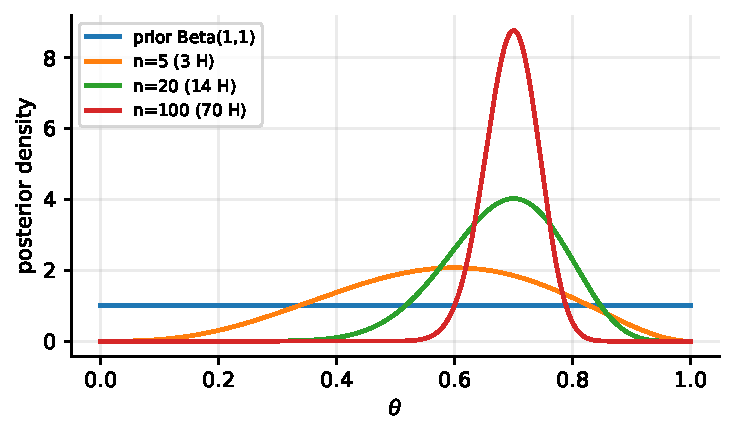
\includegraphics[width=0.9\textwidth]{gal_coin}
\caption{Learning a coin. The Beta posterior sharpens around the true bias as tosses accumulate; the prior contributes $a+b$ pseudo-observations and the predictive is the posterior mean.}
\label{fig:gal_coin}
\end{figure}

A concrete instance: a $\mathrm{Beta}(1,1)$ prior after eight heads in ten tosses gives $\mathrm{Beta}(9,3)$, posterior mean $0.75$ and a $95\%$ credible interval near $(0.48,0.94)$; the same data under a $\mathrm{Beta}(10,10)$ prior give posterior mean $0.600$, the stronger prior visibly holding the estimate back until more data arrive.


\paragraph{Learning a rate.}
For counts $y_1,\dots,y_n$ from $\mathrm{Poisson}(\theta)$ with a $\mathrm{Gamma}(a,b)$ prior on the
rate, the posterior is $\mathrm{Gamma}(a+\sum_i y_i,\,b+n)$ with mean $(a+\sum_i y_i)/(b+n)$, and the
predictive for a new count is negative binomial.
The predictive is overdispersed relative to the Poisson, because it carries the posterior
uncertainty in $\theta$ rather than fixing it.

\begin{figure}[H]
\centering
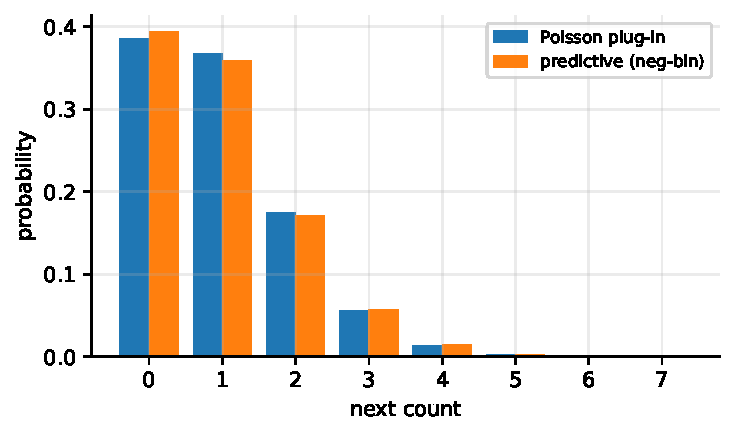
\includegraphics[width=0.9\textwidth]{gal_gammapois}
\caption{Learning a rate. The predictive count (negative binomial) is overdispersed relative to the Poisson plug-in because it carries the posterior uncertainty in the rate.}
\label{fig:gal_gammapois}
\end{figure}

A striker with eighteen goals in twenty matches under a $\mathrm{Gamma}(1,1)$ prior has posterior $\mathrm{Gamma}(19,21)$, mean $0.90$ and standard deviation $0.21$; the next-match predictive is negative binomial with the same mean but variance $0.95$, above the Poisson's $0.90$.


\paragraph{Learning a normal mean.}
With $y_i\sim\N(\theta,\sigma^2)$ and prior $\theta\sim\N(\mu_0,\tau^2)$, precisions add: the posterior
is $\N(\mu_n,\tau_n^2)$ with
\[
\frac{1}{\tau_n^2}=\frac{1}{\tau^2}+\frac{n}{\sigma^2},\qquad
\mu_n=\tau_n^2\Bigl(\frac{\mu_0}{\tau^2}+\frac{n\bar y}{\sigma^2}\Bigr),
\]
the precision-weighted average of the prior mean and the sample mean. The predictive for a new
observation is $\N(\mu_n,\sigma^2+\tau_n^2)$. As $n$ grows the data precision $n/\sigma^2$ dominates and
$\mu_n\to\bar y$, the prior washing out at rate $1/n$: this is Bernstein--von Mises for the normal mean.

\begin{figure}[H]
\centering
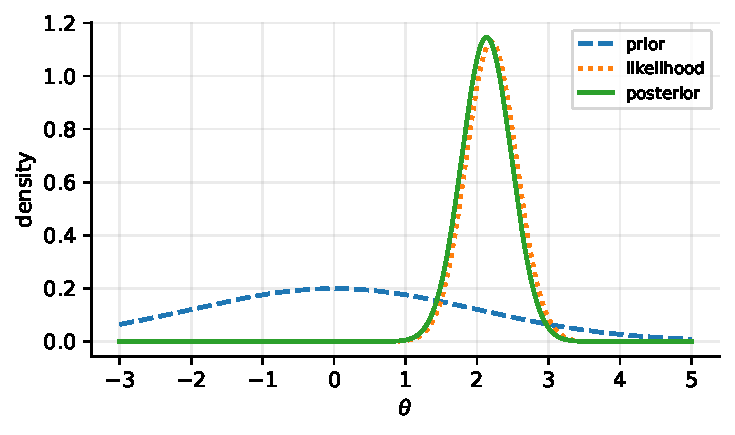
\includegraphics[width=0.9\textwidth]{gal_normalmean}
\caption{Learning a normal mean. Precisions add, so the posterior (solid) is the precision-weighted product of prior (dashed) and likelihood (dotted) and sits nearer whichever is sharper.}
\label{fig:gal_normalmean}
\end{figure}

With $\mu_0=0$, $\sigma=1$, $\tau=2$, $n=8$ and $\bar y=2.2$, the posterior precision is $1/4+8=8.25$, so the posterior is $\N(2.13,0.121)$: the prior is worth a quarter of one observation and is already almost irrelevant against eight data points.


\paragraph{Learning mean and variance together.}
When both $\theta$ and $\sigma^2$ are unknown, the conjugate normal-inverse-gamma prior gives a
normal-inverse-gamma posterior and a Student-$t$ predictive,
\[
y_{\mathrm{new}}\mid\text{data}\ \sim\ t_{2a_n}\bigl(\mu_n,\ \beta_n(1+1/\kappa_n)/a_n\bigr),
\]
with $\mu_n$, $\kappa_n$, $a_n$, $\beta_n$ the posterior mean, the prior-plus-data count, and the inverse-gamma shape and scale, so that the degrees of freedom $2a_n$ grow as data accumulate. Marginalizing the unknown scale fattens the
predictive from a normal to a $t$: the heavy tails are the honest price of not knowing the variance, and
they vanish into a normal as the degrees of freedom grow. This is the Bayesian derivation of the $t$-distribution.

\begin{figure}[H]
\centering
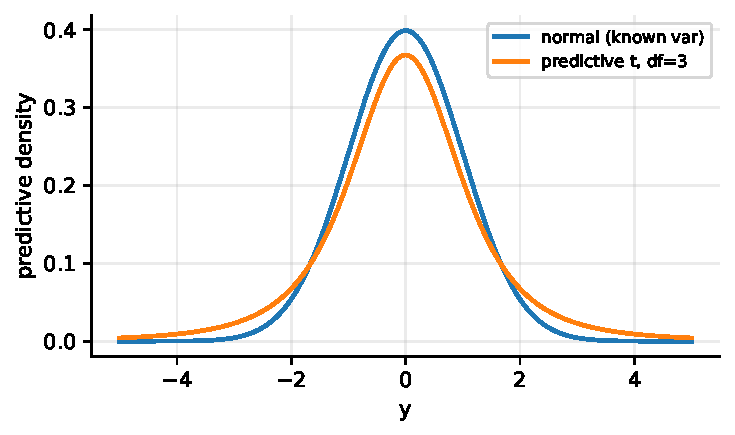
\includegraphics[width=0.9\textwidth]{gal_studentt}
\caption{Unknown variance fattens the tails. Marginalizing an unknown scale turns the Gaussian predictive into a Student-$t$, the extra tail mass being the honest cost of not knowing $\sigma^2$.}
\label{fig:gal_studentt}
\end{figure}

At $n=10$ the predictive is a $t$ on about nine degrees of freedom, whose $97.5\%$ point $2.26$ exceeds the normal's $1.96$; the interval is some fifteen percent wider purely because the scale was estimated rather than known.

\paragraph{Learning category probabilities.}
For a multinomial with cell probabilities $p$ and a $\mathrm{Dir}(\alpha)$ prior, counts $n_k$ totaling $N$
give the posterior $\mathrm{Dir}(\alpha+n)$ and the predictive
\[
\Pb(\text{next}=k\mid\text{data})=\frac{\alpha_k+n_k}{\sum_j\alpha_j+N}.
\]
Taking every $\alpha_k=1$ is add-one (Laplace) smoothing and $\alpha_k=\tfrac12$ is the
Krichevsky--Trofimov choice. This single formula is the additive smoothing at the heart of language
models and naive-Bayes classifiers: unseen categories are given the pseudo-count $\alpha_k$ rather than
probability zero.

\begin{figure}[H]
\centering
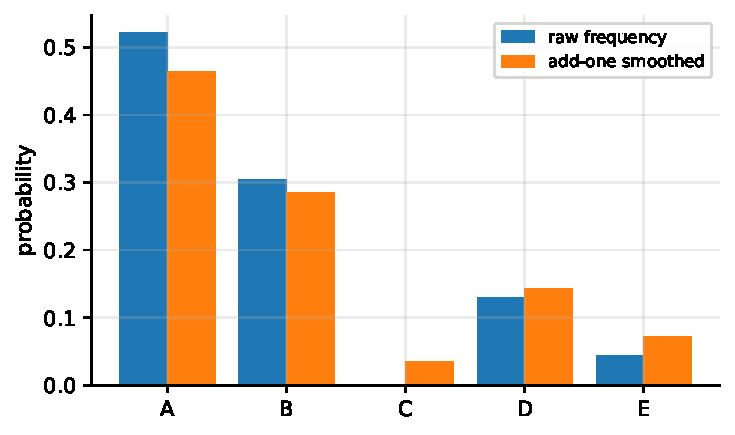
\includegraphics[width=0.9\textwidth]{gal_dirichlet}
\caption{Additive smoothing. A Dirichlet prior moves raw frequencies toward uniform, giving unseen categories the pseudo-count $\alpha_k$ instead of probability zero.}
\label{fig:gal_dirichlet}
\end{figure}

With counts $(12,7,0,3,1)$ and add-one smoothing the unseen category receives probability $1/28\approx0.036$ rather than zero, and the observed categories are shaded down just enough to make room.


\paragraph{Learning a failure rate.}
For lifetimes $y_i\sim\mathrm{Exp}(\lambda)$ with $\lambda\sim\mathrm{Gamma}(a,b)$, the posterior is
$\mathrm{Gamma}(a+n,\,b+\sum_i y_i)$ and the predictive time-to-failure is a Lomax (Pareto type II)
distribution. Reliability engineering lives here: a component that has logged many hours without failure
pushes the posterior toward small $\lambda$, and the heavy-tailed predictive warns that a long life
observed so far does not rule out an early failure next.

\begin{figure}[H]
\centering
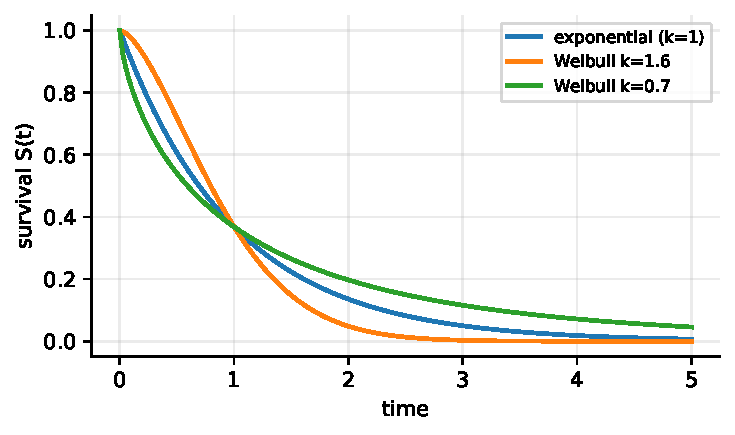
\includegraphics[width=0.9\textwidth]{gal_survival}
\caption{Reliability. The survival curve $S(t)=e^{-(\lambda t)^k}$ bends with the Weibull shape $k$; conjugate gamma-exponential updating learns the rate from censored lifetimes.}
\label{fig:gal_survival}
\end{figure}

A Weibull shape above one models wear-out and below one infant mortality; in the exponential case $k=1$ with censoring, the conjugate gamma update needs only the total time on test and the number of failures.


\paragraph{Overdispersion by a beta mixture.}
If each group's success probability is itself drawn $\theta_g\sim\mathrm{Beta}(a,b)$ and then
$y_g\sim\mathrm{Bin}(m,\theta_g)$, the marginal count is beta-binomial with variance
$m\bar\theta(1-\bar\theta)\{1+(m-1)\rho\}$ for $\bar\theta=a/(a+b)$, inflated over the binomial by the intraclass correlation
$\rho=1/(a+b+1)$. The lesson is that a hierarchical prior on a rate is a model for
extra-binomial variation, and the correlation it induces is the shrinkage the hierarchy will later apply.

\begin{figure}[H]
\centering
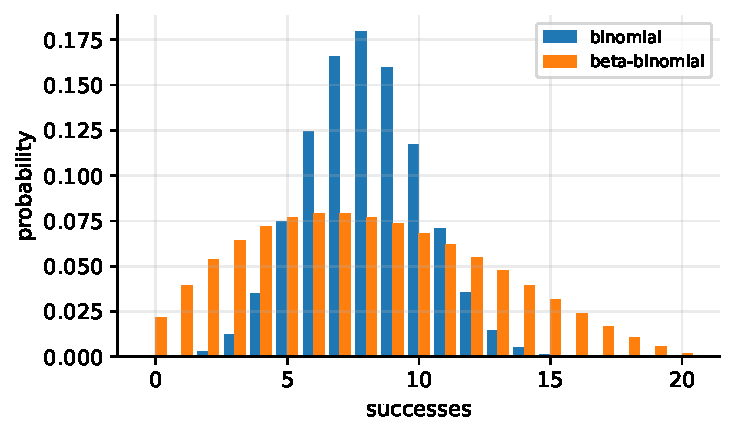
\includegraphics[width=0.9\textwidth]{gal_betabinom}
\caption{Overdispersion. A beta mixture spreads the count distribution wider than the binomial of the same mean, the extra variance being the intraclass correlation.}
\label{fig:gal_betabinom}
\end{figure}

With $m=20$ trials and $\mathrm{Beta}(2,3)$ mixing the intraclass correlation is $1/(2+3+1)=1/6$, so the count variance is inflated by the factor $1+(m-1)/6\approx4.2$ over the binomial of the same mean.

\section*{Classic named problems}

\paragraph{The German tank problem.}
From serial numbers $1,\dots,N$ a sample of size $k$ has maximum $m$. With a scale-free prior on $N$
the posterior concentrates just above $m$, and the posterior mean is close to the unbiased frequentist
estimate $m(1+1/k)-1$; both add to the observed maximum a correction of order $m/k$ for the gap above
the largest serial seen. Estimating a population size from the largest label in a sample is the pattern,
and the Bayesian and frequentist answers agree to leading order while differing in how they express the
residual uncertainty.

\begin{figure}[H]
\centering
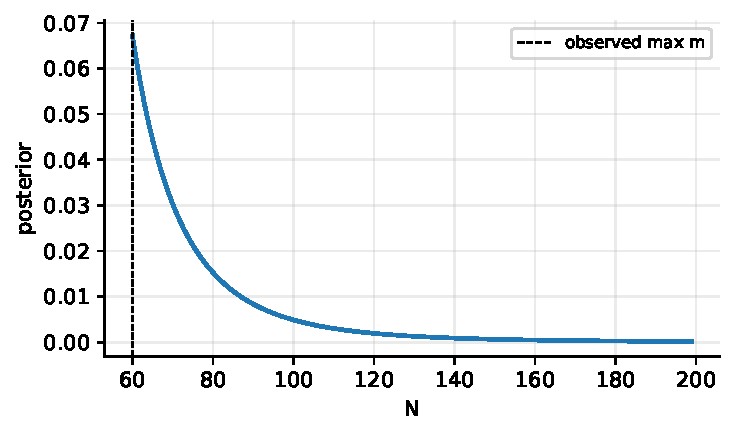
\includegraphics[width=0.9\textwidth]{gal_tank}
\caption{The German tank problem. The posterior over the population size $N$ concentrates just above the observed maximum serial number, with a tail set by the sample size.}
\label{fig:gal_tank}
\end{figure}

A maximum serial of sixty in a sample of five gives the frequentist unbiased estimate of seventy-one and a Bayesian posterior mean a few units higher, and the posterior width shrinks like $1/k$ with each further captured unit.


\paragraph{The taxicab problem.}
Seeing a single taxi numbered $m$ in a town with an unknown number $N\ge m$ of taxis, a scale-invariant
prior $\Pi(N)\propto 1/N$ gives a posterior $\propto 1/N^2$ on $N\ge m$ with median near $2m$ but
infinite mean. One observation is thin evidence: the answer depends visibly on the prior, and the
divergent mean is a caution that an improper prior can leave a posterior functional undefined even when
the posterior itself is proper.

\paragraph{Naive Bayes classification.}
Assigning a document to class $c$ uses the log-posterior
\[
\log\Pb(c\mid x)=\log\pi_c+\sum_j\log p(x_j\mid c)+\text{const},
\]
additive over features under the assumption that features are conditionally independent given the
class, and linear in the feature counts for multinomial features. The independence assumption is almost always false, yet the classifier is famously effective,
because the decision boundary depends only on the sign of a log-odds that the wrong correlations rarely
flip. Naive Bayes is the simplest predictive model that still learns, and it is a Dirichlet-multinomial update run per class.

\begin{figure}[H]
\centering
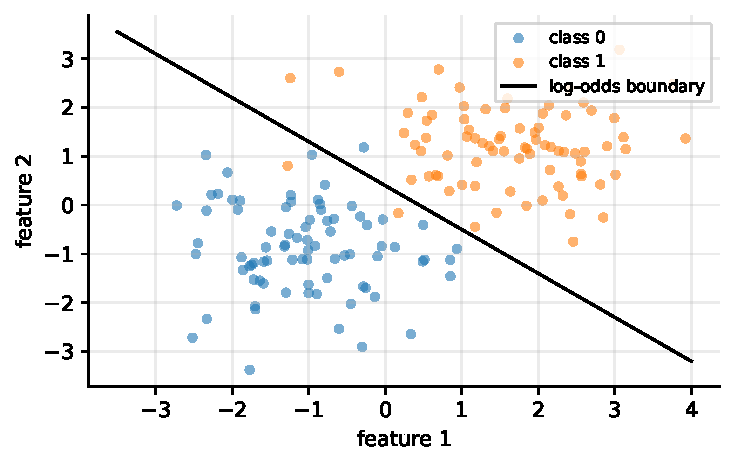
\includegraphics[width=0.9\textwidth]{gal_naivebayes}
\caption{Naive Bayes. Conditional independence makes the log-odds a sum of one term per feature; for Gaussian features whose variances the two classes share, as sketched here, each term is linear, so the decision boundary is a line (a hyperplane in more dimensions) even when the class densities are crude. Variances that differ between the classes would make it quadratic.}
\label{fig:gal_naivebayes}
\end{figure}

Even with correlated features the classifier errs only when the accumulated log-odds crosses zero, which redundant evidence rarely forces, so accuracy survives the false independence assumption.

\paragraph{Bayesian linear regression and ridge as a prior.}
For $y=X\beta+\varepsilon$ with $\varepsilon\sim\N(0,\sigma^2 I)$ and prior $\beta\sim\N(0,\tau^2 I)$,
the posterior mean is
\[
\hat\beta=(X^\top X+\lambda I)^{-1}X^\top y,\qquad \lambda=\sigma^2/\tau^2,
\]
the ridge estimate, and the predictive variance inflates by the parameter uncertainty
$x_\star^\top(X^\top X+\lambda I)^{-1}x_\star\,\sigma^2$. Ridge regression is therefore a Gaussian-prior
MAP, and its penalty is a variance ratio: a tighter prior (small $\tau$) shrinks harder. The Bayesian
version adds the honest predictive intervals the point estimate omits.

\begin{figure}[H]
\centering
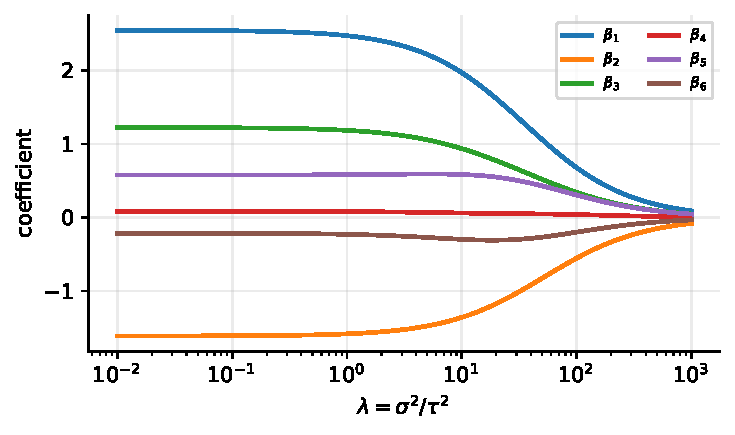
\includegraphics[width=0.9\textwidth]{gal_ridge}
\caption{Ridge as a Gaussian prior. As the prior tightens (larger $\lambda=\sigma^2/\tau^2$) every coefficient is shrunk toward zero along a smooth path.}
\label{fig:gal_ridge}
\end{figure}

As $\lambda\to0$ the ridge fit returns least squares and as $\lambda\to\infty$ it collapses to the prior mean zero; the evidence picks the $\lambda$ that balances fidelity against shrinkage, and it is a variance ratio, not a free knob.


\paragraph{Bayesian A/B testing.}
Two variants with beta-Bernoulli posteriors $\mathrm{Beta}(a_A,b_A)$ and $\mathrm{Beta}(a_B,b_B)$ are
compared by the posterior probability $\Pb(\theta_A>\theta_B\mid\text{data})$ and by the expected loss of
shipping the worse arm, $\E[(\theta_B-\theta_A)^+\mid\text{data}]$. Reporting these two numbers, a
probability of being better and a cost of being wrong, replaces a significance test with a decision, and
it is the quantity Thompson sampling turns into an allocation rule.

\begin{figure}[H]
\centering
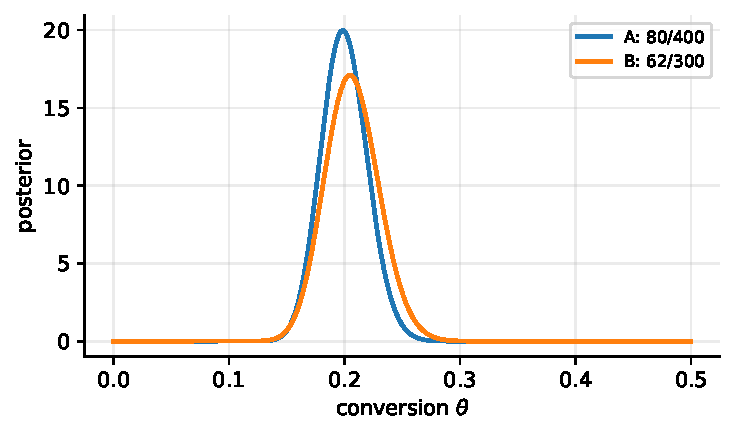
\includegraphics[width=0.9\textwidth]{gal_ab}
\caption{A/B testing. The arms' Beta posteriors overlap; the decision reads off $\Pb(\theta_A>\theta_B)$ and the expected loss of shipping the worse arm.}
\label{fig:gal_ab}
\end{figure}

With arm A at $80/400$ and arm B at $62/300$ under the improper $\mathrm{Beta}(0,0)$ prior on each arm, the posteriors are $\mathrm{Beta}(80,320)$ and $\mathrm{Beta}(62,238)$; simulation gives $\Pb(\theta_A>\theta_B)\approx0.42$, so B is more likely the better arm, and the expected loss from shipping A, $\E[(\theta_B-\theta_A)^+]$, is about $1.6$ percentage points.


\paragraph{James--Stein shrinkage and empirical Bayes.}
For $y_i\sim\N(\theta_i,1)$, $i=1,\dots,p$, the James--Stein estimator
\[
\hat\theta_i=\Bigl(1-\frac{p-2}{\lVert y\rVert^2}\Bigr)y_i
\]
dominates the maximum likelihood estimate $y_i$ in total squared error for $p\ge3$, Stein's paradox. It
is the empirical-Bayes posterior mean under $\theta_i\sim\N(0,\tau^2)$ with $\tau^2$ estimated from
$\lVert y\rVert^2$: the data supply the shrinkage factor. Borrowing strength across coordinates beats
treating them separately, the practical moral that hierarchical models formalize.

\begin{figure}[H]
\centering
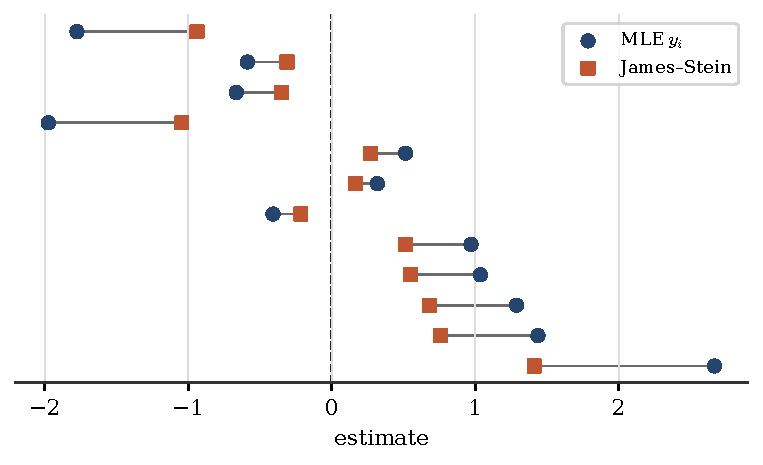
\includegraphics[width=0.9\textwidth]{gal_js}
\caption{Stein shrinkage. Each maximum-likelihood estimate (circles) is pulled toward the origin (squares); the total squared error of the shrunk estimates is smaller on average once $p\ge3$.}
\label{fig:gal_js}
\end{figure}

For the $p=12$ coordinates of Figure~\ref{fig:gal_js}, whose means $\theta_i$ are the quantiles of $\N(0,\tfrac32)$ at levels $(i-\tfrac12)/12$, the draw has $\lVert y\rVert^2\approx21.2$, so the shrinkage factor $1-(p-2)/\lVert y\rVert^2\approx0.53$ pulls every estimate nearly half of the way to the origin. At these means the expected summed squared error is $8.0$, below the $12$ of the raw maximum likelihood estimate, though in this draw, whose noise happens to be small, the James--Stein summed squared error ($4.85$) is no better than the raw estimate's ($4.77$).


\paragraph{Batting averages: shrinkage on real data.}
Efron and Morris shrank the early-season batting averages of eighteen players toward their grand mean and
predicted the rest of the season better than the raw averages did, for all but two players. The estimator
is the eight-schools shrinkage of the main text applied to a binomial rate: each average is pulled toward
the common mean by a weight set by the within-player noise relative to the between-player spread. It is
the most cited demonstration that pooling improves prediction.

\begin{figure}[H]
\centering
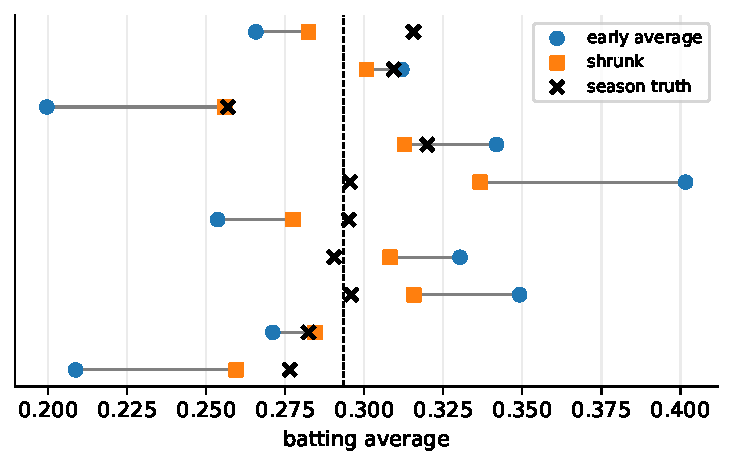
\includegraphics[width=0.9\textwidth]{gal_batting}
\caption{Batting averages. Early-season rates (circles) are shrunk toward the grand mean (squares), landing closer to the end-of-season truth (crosses) than the raw averages do.}
\label{fig:gal_batting}
\end{figure}


\section*{Prediction, coding, and sequential learning}

\paragraph{The Krichevsky--Trofimov predictor.}
The add-one-half rule $\Pb(\text{next}=1\mid\text{data})=(k+\tfrac12)/(n+1)$ is the predictive under a
$\mathrm{Beta}(\tfrac12,\tfrac12)$ (Jeffreys) prior, and its cumulative log-loss exceeds that of the best
fixed Bernoulli model by only $\tfrac12\log n+O(1)$. This redundancy is minimax to leading order, so the Jeffreys prior is
a rate-optimal universal predictor for a coin, and the $\tfrac12\log n$ is the same per-parameter code-length
that BIC charges. Universal prediction and description length meet at the same reference prior.

\begin{figure}[H]
\centering
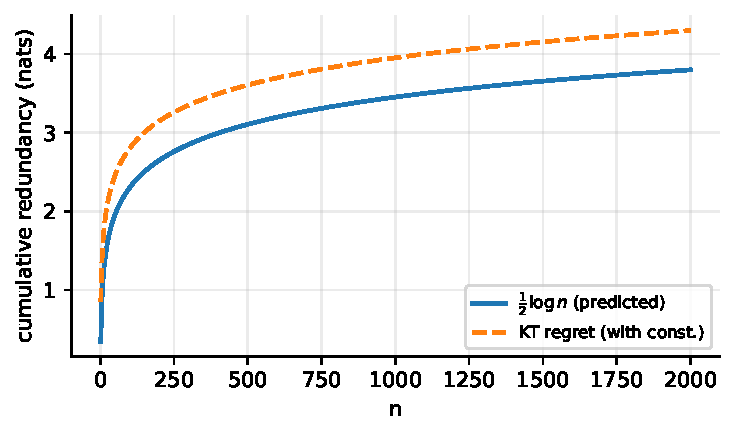
\includegraphics[width=0.9\textwidth]{gal_kt}
\caption{Universal prediction. The cumulative log-loss regret of the Krichevsky--Trofimov predictor tracks $\tfrac12\log n$, the same per-parameter penalty BIC charges.}
\label{fig:gal_kt}
\end{figure}

Summed over a thousand tosses of a fair coin, the add-one-half predictor's log-loss exceeds the best fixed Bernoulli code by about $\tfrac12\log 1000+\tfrac12\log\tfrac\pi2\approx3.68$ nats on average, matching the $\tfrac12\log n+O(1)$ redundancy the theory predicts.


\paragraph{Sequential updating and the likelihood principle.}
Because the posterior after $n$ observations depends on the data only through the likelihood, updating
one datum at a time and updating in a single batch give the identical posterior, and a stopping rule that
depends only on observed data leaves the likelihood, and hence the inference, unchanged. This coherence,
that when one looks does not alter what one should believe, is the sharpest contrast with frequentist
procedures whose error rates depend on the sampling plan, and it is why the e-process of
Section~\ref{ch:evalues} needs no correction for optional stopping.

\begin{figure}[H]
\centering
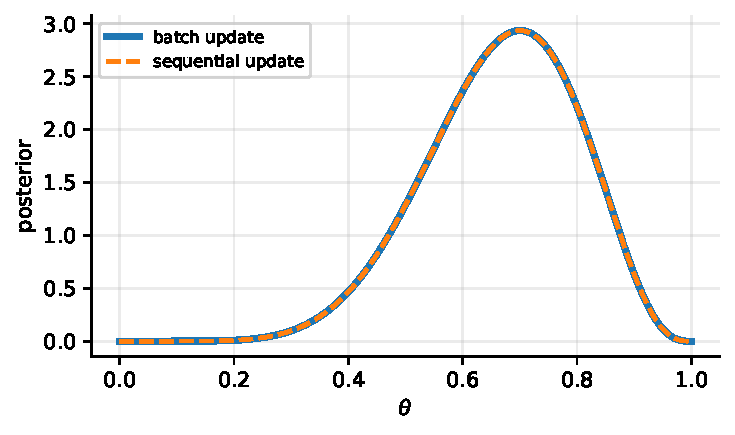
\includegraphics[width=0.9\textwidth]{gal_likelihood}
\caption{The likelihood principle. Updating one datum at a time and in a single batch give the identical posterior, so when one looks does not alter what one should believe.}
\label{fig:gal_likelihood}
\end{figure}

A trial stopped early for success and one run to a fixed size yield the same posterior from the same counts, so optional stopping needs no penalty.


\paragraph{Bayes mixtures and universal prediction.}
Predicting a sequence with a Bayes mixture $\Pb(x_{1:n})=\int\prod_i p(x_i\mid\theta)\,d\Pi(\theta)$
incurs cumulative log-loss regret against the best model in the class that grows, like the mutual information
between parameter and data, as $\tfrac d2\log n$ for a $d$-parameter smooth family. The
mixture forecaster is therefore never much worse than the best hindsight model, and its regret is the
evidence penalty once more. A good compressor and a good forecaster are the same object.

\begin{figure}[H]
\centering
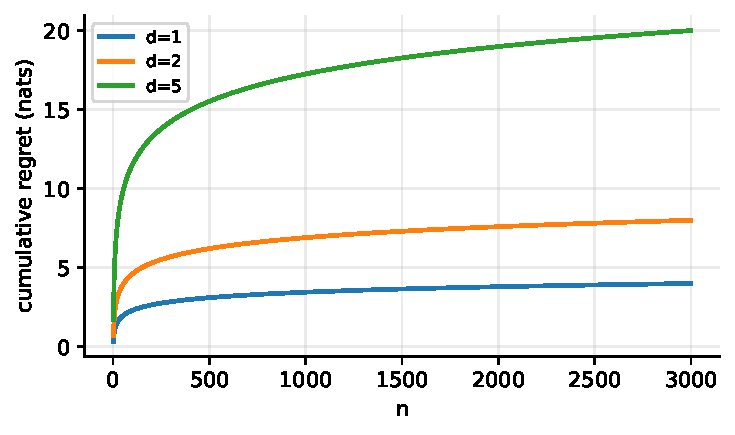
\includegraphics[width=0.9\textwidth]{gal_mixture}
\caption{Universal prediction. The Bayes-mixture regret against the best model in a $d$-parameter class grows as $\tfrac{d}{2}\log n$, the evidence penalty seen once more.}
\label{fig:gal_mixture}
\end{figure}


\paragraph{P\'olya's urn and where exchangeability comes from.}
An urn with $a$ red and $b$ black balls, each draw replaced together with one more of the color drawn,
generates an exchangeable binary sequence whose limiting red fraction is $\mathrm{Beta}(a,b)$. The urn
\emph{is} the de Finetti representation made mechanical: the reinforcement creates the exchangeable
correlations, and the mixing measure is the law of the long-run frequency. Beta-Bernoulli learning and
P\'olya's urn are the same process read forward and backward.

\begin{figure}[H]
\centering
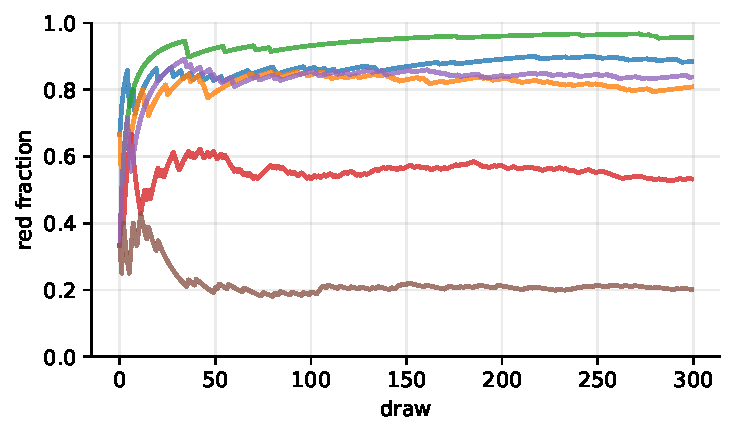
\includegraphics[width=0.9\textwidth]{gal_polya}
\caption{Where exchangeability comes from. Reinforced draws from a P\'olya urn have red fractions that converge to distinct Beta-distributed limits, one directing measure per path.}
\label{fig:gal_polya}
\end{figure}

From one ball of each color the limiting red fraction is uniform on $(0,1)$, so different runs converge to entirely different frequencies; the urn draws the mixing measure first and the sequence second.


\section*{Concentration and generalization: how fast do we learn?}

\paragraph{How many samples to learn a probability?}
Estimating a probability $p$ by the empirical frequency $\hat p$ from $n$ independent Bernoulli draws,
Hoeffding's inequality (Hoeffding, 1963) gives the distribution-free bound
\[
\Pb\bigl(|\hat p-p|\ge\varepsilon\bigr)\le 2e^{-2n\varepsilon^2},
\]
so $n\ge\frac{1}{2\varepsilon^2}\log\frac{2}{\delta}$ draws guarantee accuracy $\varepsilon$ with
confidence $1-\delta$. The
bound is the frequentist companion of the beta-Bernoulli posterior, whose width $\sqrt{p(1-p)/n}$ shrinks
at the same $1/\sqrt n$ rate: concentration says the learning happens, and at what speed.

\begin{figure}[H]
\centering
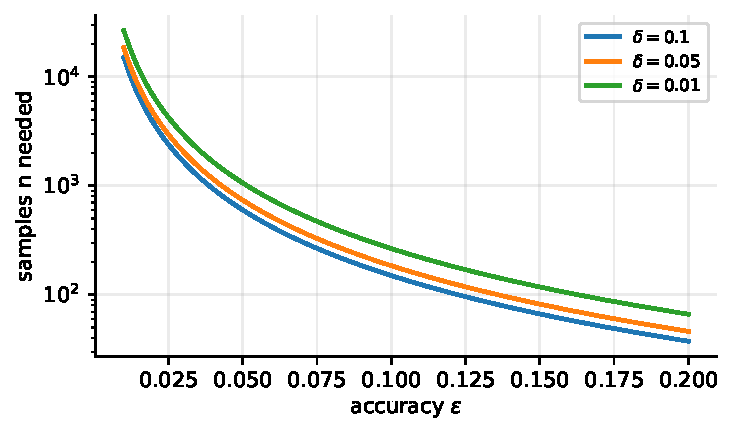
\includegraphics[width=0.9\textwidth]{gal_hoeffding}
\caption{Sample complexity. Hoeffding's bound $2e^{-2n\varepsilon^2}$ fixes the number of draws needed to estimate a probability to accuracy $\varepsilon$ with confidence $1-\delta$.}
\label{fig:gal_hoeffding}
\end{figure}

Read backward, the bound says that estimating a probability to within $0.01$ at $95\%$ confidence needs $n\ge\log(40)/(2\cdot0.01^2)\approx18{,}400$ draws, a figure that does not depend on the unknown $p$.


\paragraph{A PAC-Bayes generalization bound.}
For any data-dependent posterior $Q$ and fixed prior $P$ over predictors, with probability at least
$1-\delta$ the gap between true and empirical risk of the Gibbs classifier is bounded by
\[
\mathrm{risk}(Q)-\widehat{\mathrm{risk}}(Q)\ \le\ \sqrt{\frac{\D{Q}{P}+\log(2\sqrt n/\delta)}{2n}},
\]
the bound of McAllester (2003) in the form of Maurer (2004). It follows by a change-of-measure step
from $\E\exp(2n\Delta^2)\le2\sqrt n$ for the gap $\Delta$ of a fixed predictor with loss in $[0,1]$, Maurer's sharpening of Hoeffding's inequality (Hoeffding, 1963). Generalization is thus governed by the relative entropy between what the data
taught ($Q$) and what was assumed ($P$): the same Kullback--Leibler divergence that prices evidence and
sets the deviation rate throughout this book here bounds out-of-sample error.

\paragraph{Occam's razor by integration.}
A model that can fit many datasets must spread its predictive mass thin, so the datasets it does fit it
fits only weakly; the evidence $\int p(D\mid\theta)\,\pi(\theta)\,d\theta$ rewards a model that predicts
the observed data sharply without needing to be tuned. This automatic penalty, the Occam factor of
Section~\ref{ch:mdl}, is why integrating over parameters, rather than maximizing over them, avoids
overfitting without a separate validation set.

\begin{figure}[H]
\centering
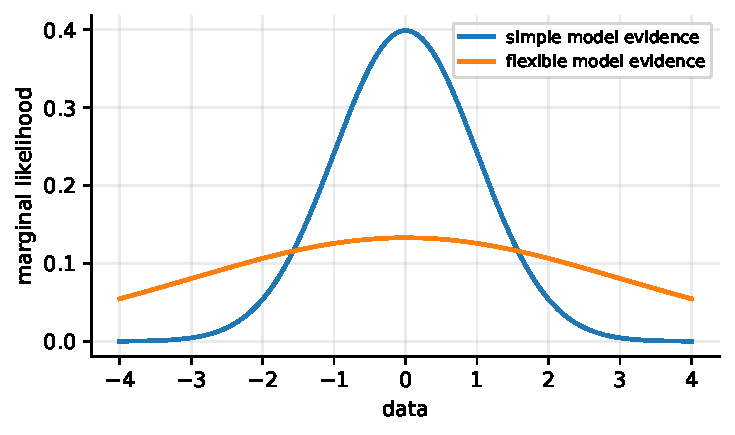
\includegraphics[width=0.9\textwidth]{gal_occam}
\caption{Occam's razor by integration. A flexible model spreads its marginal likelihood over many datasets and so predicts any one of them less sharply than a simple model that fits.}
\label{fig:gal_occam}
\end{figure}

Two nested models can tie in fit yet not in evidence: the flexible one pays for reach it did not use, so the Bayes factor favors the simpler model until the data demand otherwise.


\section*{Decision: turning the posterior into an action}

\paragraph{The loss chooses the summary.}
The Bayes act under squared-error loss is the posterior mean, under absolute loss the posterior median,
and under $0/1$ loss the posterior mode. A single posterior therefore yields three different point
estimates depending on how errors are priced, which is why reporting a posterior, rather than one number,
is the honest output of inference.

\begin{figure}[H]
\centering
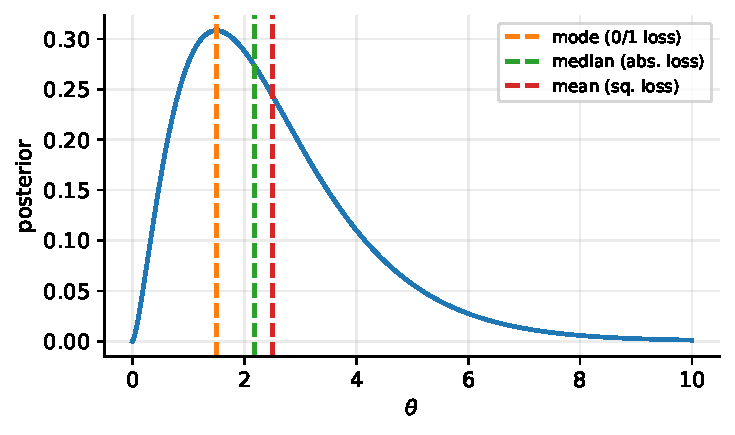
\includegraphics[width=0.9\textwidth]{gal_loss}
\caption{The loss chooses the summary. On a skewed posterior the Bayes act is the mean under squared error, the median under absolute error, and the mode under $0/1$ loss.}
\label{fig:gal_loss}
\end{figure}

On a right-skewed posterior the mode, median and mean fall in that order, so the choice of loss can move the reported estimate noticeably, which is why the loss must be named first.


\paragraph{The Bayesian newsvendor.}
Stocking $q$ units against uncertain demand with unit underage cost $c_u$ and overage cost $c_o$, the
expected-loss-minimizing order is the critical-fractile quantile of the \emph{predictive} demand
distribution,
\[
q^\star=F^{-1}_{\mathrm{pred}}\Bigl(\frac{c_u}{c_u+c_o}\Bigr).
\]
The decision reads a quantile of the predictive, not its mean, and carrying the posterior uncertainty
widens the predictive and shifts the order. Whenever the loss is asymmetric it is the predictive
distribution, and not a point forecast, that the decision needs.

\begin{figure}[H]
\centering
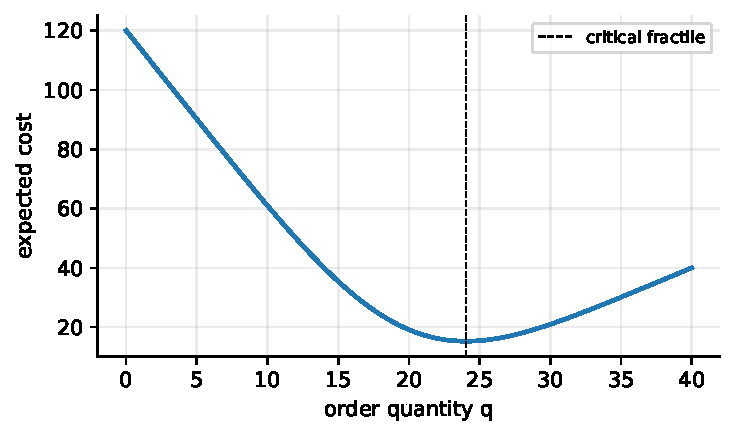
\includegraphics[width=0.9\textwidth]{gal_newsvendor}
\caption{A quantile decision. The expected-cost-minimizing order is the critical-fractile quantile of the predictive demand, not its mean.}
\label{fig:gal_newsvendor}
\end{figure}

With underage cost six, overage cost two and demand $\N(20,6^2)$, the critical fractile is $6/8=0.75$, so the order is the third-quartile demand, about twenty-four units, four above the mean because running short is dearer than overstocking.


\paragraph{Wald's sequential probability ratio test.}
Accumulating the log-likelihood ratio $S_n=\sum_i\log\{p_1(x_i)/p_0(x_i)\}$ and stopping when it crosses
$\log A$ or $\log B$ gives a test whose expected sample size under $H_1$ is
$\E_1[N]\approx(\log A)/\D{P_1}{P_0}$, the boundary divided by the information per observation. The
classic SPRT is the growth-optimal sequential test, and the e-process of Section~\ref{ch:evalues} is its
prior-free, anytime-valid descendant.

\begin{figure}[H]
\centering
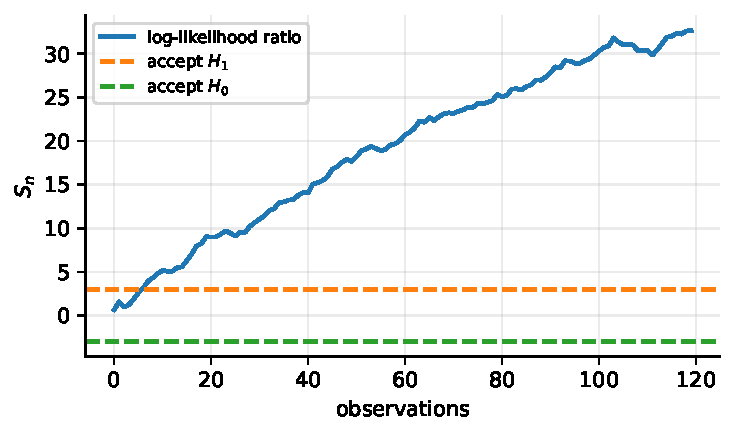
\includegraphics[width=0.9\textwidth]{gal_wald}
\caption{Wald's sequential test. The log-likelihood ratio is a random walk stopped at two boundaries; the expected sample size is the boundary divided by the information per observation.}
\label{fig:gal_wald}
\end{figure}

Setting the boundaries to $1/\alpha$ and $\beta$ bounds the type I and type II error rates by $\alpha$ and $\beta$, and the SPRT's expected sample size is the smallest among all tests whose error rates are no larger than its own, Wald's optimality theorem.



\section*{Conjugate families in general}

\paragraph{The exponential-family master pattern.}
Every conjugate update above is one pattern. If $p(y\mid\eta)=h(y)\exp\{\eta^\top T(y)-A(\eta)\}$ is an
exponential family and the prior is the conjugate $\pi(\eta)\propto\exp\{\eta^\top\chi-\nu A(\eta)\}$,
then after data $y_{1:n}$ the posterior is again conjugate with
\[
\chi\ \mapsto\ \chi+\sum_i T(y_i),\qquad \nu\ \mapsto\ \nu+n.
\]
Learning is bookkeeping on two hyperparameters: the accumulated sufficient statistic and the count of
observations. Beta-Bernoulli, gamma-Poisson, normal-normal, and Dirichlet-multinomial are this one line
specialized, and the posterior mean of the mean parameter is always a convex blend of the prior guess and
the sample statistic.

\begin{figure}[H]
\centering
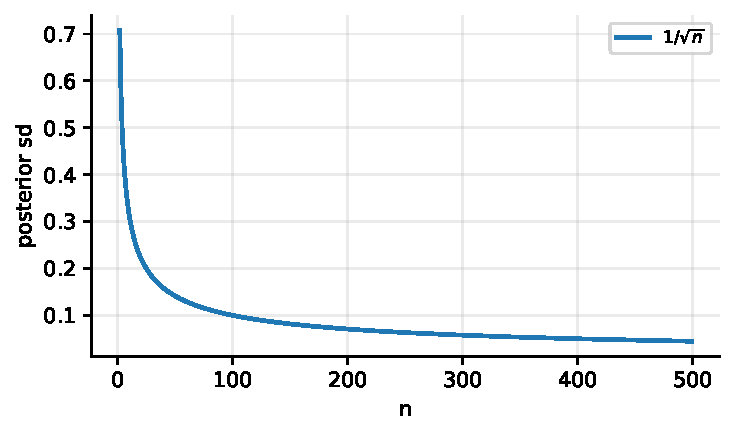
\includegraphics[width=0.9\textwidth]{gal_contraction}
\caption{Posterior contraction. Under conjugate updating the posterior standard deviation falls like $1/\sqrt{n}$, the parametric learning rate.}
\label{fig:gal_contraction}
\end{figure}

Because the width falls like $1/\sqrt n$, halving a credible interval takes four times the data; reaching a half-width of $0.05$ for a proportion near one-half needs on the order of a few hundred observations.


\paragraph{Learning a covariance.}
For $y_i\sim\N_d(\mu,\Sigma)$ with $\mu$ known and an inverse-Wishart prior on $\Sigma$, the posterior is inverse-Wishart
with the prior scale matrix updated by the sample scatter $\sum_i(y_i-\mu)(y_i-\mu)^\top$ and the
degrees of freedom increased by $n$, and the predictive is a multivariate Student-$t$. With $\mu$ also unknown and the prior $\mu\mid\Sigma\sim\N_d(\mu_0,\Sigma/\kappa_0)$ (normal-inverse-Wishart), the scatter is taken about $\bar y$ and gains the rank-one term $\tfrac{\kappa_0n}{\kappa_0+n}(\bar y-\mu_0)(\bar y-\mu_0)^\top$, the degrees of freedom still rise by $n$, and the predictive is again a multivariate
Student-$t$. Estimating a covariance is the matrix version of learning a variance, and the
inverse-Wishart prior is a bundle of prior pseudo-observations whose scatter is the prior scale.

\begin{figure}[H]
\centering
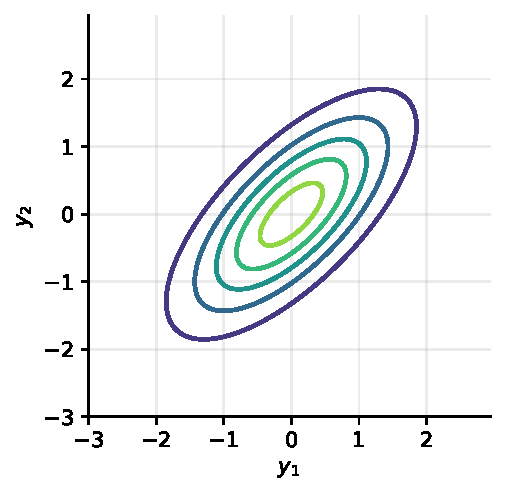
\includegraphics[width=0.9\textwidth]{gal_cov}
\caption{Learning a covariance. An inverse-Wishart prior updates its scale by the sample scatter; the contours show the learned correlation structure of a bivariate normal.}
\label{fig:gal_cov}
\end{figure}

The inverse-Wishart degrees of freedom act as a prior sample size, and the posterior estimate of the covariance is a sample-size-weighted blend of the prior scale and the observed scatter.


\section*{Time and state}

\paragraph{The Kalman filter as recursive Bayes.}
The linear-Gaussian filter is conjugate normal-normal updating repeated in time: the one-step predictive
$\N(F\hat x_{t-1},FP_{t-1}F^\top+Q)$ plays the role of the prior, the observation plays the role of one
datum, and Bayes' rule returns the Gaussian posterior $\N(\hat x_t,P_t)$. Filtering is therefore Bayesian
learning with a moving target, and the Kalman gain is the precision weight deciding how much of each new observation to believe.

\begin{figure}[H]
\centering
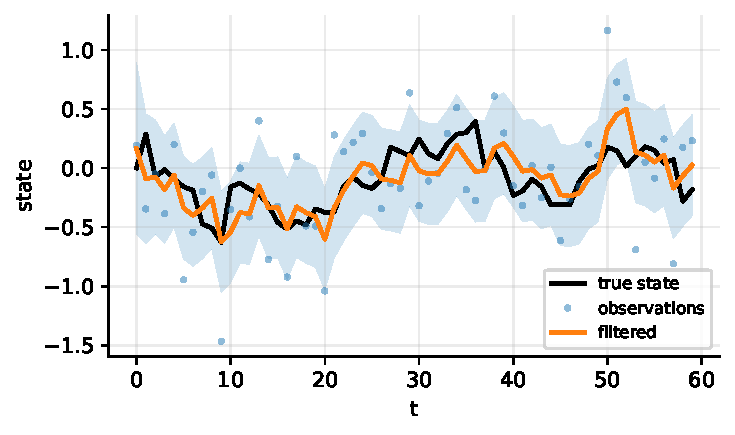
\includegraphics[width=0.9\textwidth]{gal_kalman}
\caption{The Kalman filter as recursive Bayes. Conjugate normal updating in time tracks the latent state (black) from noisy observations (dots), the credible band shrinking as information accrues.}
\label{fig:gal_kalman}
\end{figure}

The steady-state gain solves a scalar Riccati equation, and once reached the filter is a fixed exponential smoother: each estimate is a geometrically weighted average of past observations, with the decay rate set by the ratio of process to observation noise.

\paragraph{Hidden Markov models and the forward algorithm.}
For a discrete latent state evolving by a transition matrix and emitting observations, the forward
recursion propagates $\Pb(\text{state}_t\mid y_{1:t})\propto p(y_t\mid\text{state}_t)\sum_{s}
\Pb(\text{state}_{t-1}=s\mid y_{1:t-1})\,\Pb(\text{state}_t\mid\text{state}_{t-1}=s)$. This is exact Bayesian filtering over a
finite state space, the discrete cousin of the Kalman filter, and it is the engine of speech, genomics,
and part-of-speech tagging.

\begin{figure}[H]
\centering
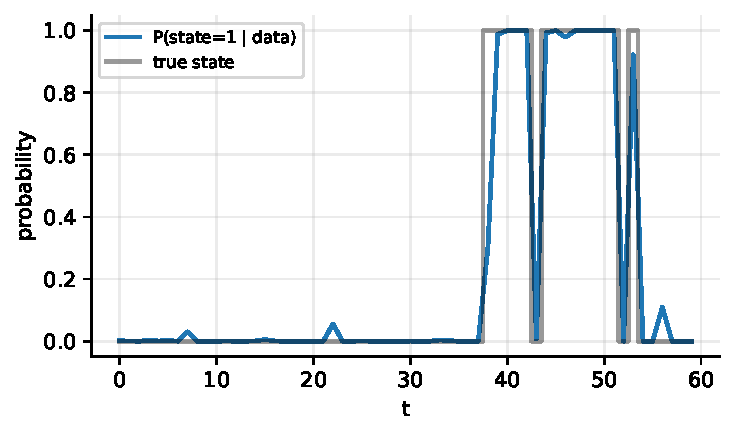
\includegraphics[width=0.9\textwidth]{gal_hmm}
\caption{Discrete filtering. The forward algorithm's posterior over the latent state (curve) follows the true state (steps), the discrete cousin of the Kalman filter.}
\label{fig:gal_hmm}
\end{figure}

The same forward pass returns the evidence $\Pb(y_{1:T})$ as the product of the normalizing constants along the way, so filtering and model comparison share one recursion.


\paragraph{Online change-point detection.}
Placing a geometric prior on the run length since the last change and updating it against a conjugate
predictive gives an exact recursive posterior over the time since the most recent change point. Learning
here is learning \emph{when} the world changed, and the run-length posterior is a coherent alarm that
sharpens as evidence for a break accumulates.

\begin{figure}[H]
\centering
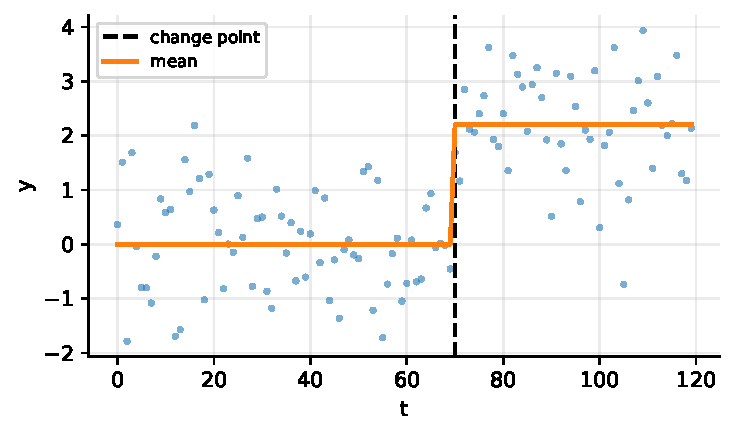
\includegraphics[width=0.9\textwidth]{gal_changepoint}
\caption{Change-point detection. A run-length posterior over the time since the last change sharpens into an alarm as evidence for a break accumulates.}
\label{fig:gal_changepoint}
\end{figure}

The run-length posterior keeps its mass at large values while the process is stable and collapses toward zero when a break occurs, and that collapse is the detection signal.


\section*{Latent structure}

\paragraph{Mixtures and the EM algorithm.}
A finite mixture with latent labels $z_i$ is fit by alternating the expected responsibilities
$\Pb(z_i=k\mid y_i,\theta)$ with the conjugate updates they imply, which is EM, and adding a prior
turns it into MAP-EM. EM is coordinate ascent on the same evidence lower bound Section~\ref{ch:vi}
uses, so the classic clustering algorithm is a special case of the book's entropy-regularized prediction.

\begin{figure}[H]
\centering
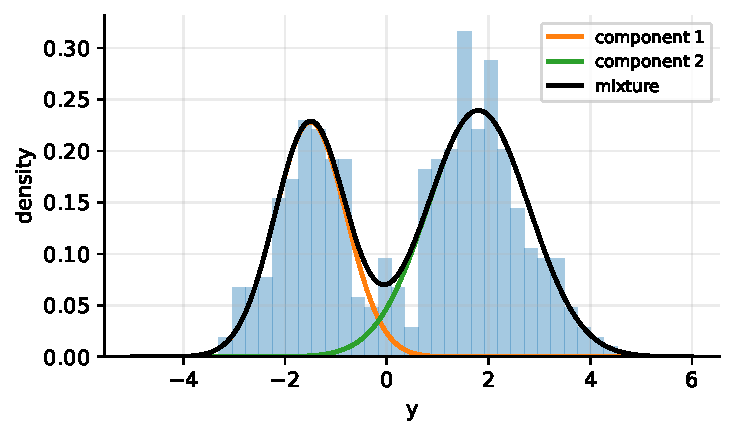
\includegraphics[width=0.9\textwidth]{gal_em}
\caption{Mixtures and EM. Alternating responsibilities with conjugate updates fits a Gaussian mixture; EM is coordinate ascent on the evidence lower bound.}
\label{fig:gal_em}
\end{figure}

Each step cannot lower the likelihood, so EM climbs to a local optimum; a few restarts guard against poor optima.


\paragraph{Topic models as hierarchical Dirichlet-multinomial.}
Latent Dirichlet allocation gives each document a Dirichlet mix of topics and each topic a Dirichlet
distribution over words, and inference is repeated Dirichlet-multinomial updating over the latent
word-to-topic assignments. It is naive Bayes with the class made latent and given a Dirichlet prior, and
it learns the topics and the mixtures together.

\begin{figure}[H]
\centering
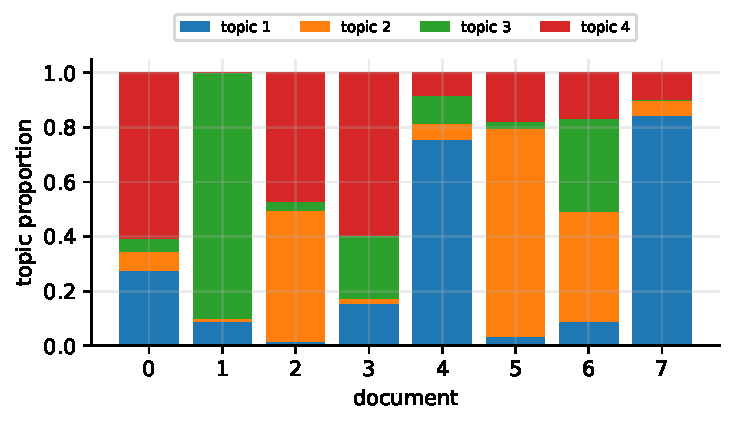
\includegraphics[width=0.9\textwidth]{gal_lda}
\caption{Topic models. Latent Dirichlet allocation gives each document a Dirichlet mixture over topics; inference is Dirichlet-multinomial updating over latent assignments.}
\label{fig:gal_lda}
\end{figure}

The Dirichlet concentration sets how peaked a document's topic vector is: small values give documents about a single topic, large values even blends.


\section*{Functions and nonparametrics}

\paragraph{Smoothing splines as a Gaussian process.}
Penalizing the integrated squared second derivative of a regression function is the same as placing a
Gaussian-process prior with the corresponding covariance, so the smoothing spline is the posterior mean
of a Gaussian process and the smoothing parameter is a variance ratio chosen by the evidence. Regularized
curve fitting is Bayesian function learning in disguise.

\begin{figure}[H]
\centering
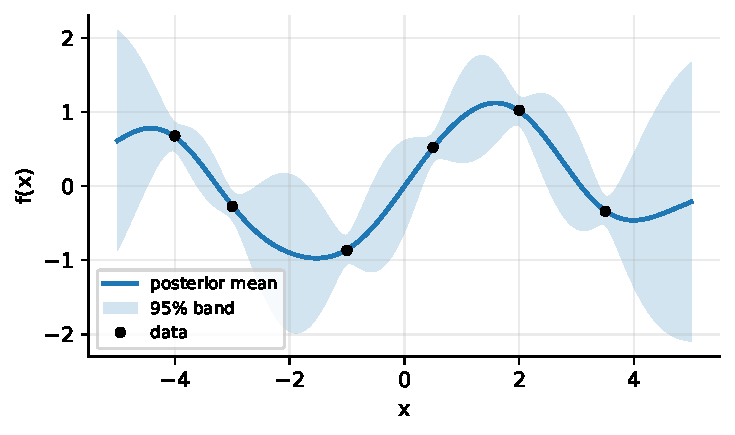
\includegraphics[width=0.9\textwidth]{gal_gp}
\caption{Function learning. The Gaussian-process posterior mean interpolates the data with a credible band that widens away from observations; the smoothing spline is its posterior mean.}
\label{fig:gal_gp}
\end{figure}

The posterior mean is a weighted sum of kernels centered at the data, $\sum_i\alpha_i k(x,x_i)$, and the band is widest midway between observations, where a spline is least constrained.


\paragraph{Gaussian-process classification.}
Putting a Gaussian-process prior on a latent function with a logistic link gives a nonparametric
classifier whose posterior is no longer Gaussian; a single P\'olya--Gamma augmentation or a Laplace
approximation restores tractable updates. The predictive class probability then carries the function
uncertainty, so the model reports where it does not know rather than only where the boundary lies.

\begin{figure}[H]
\centering
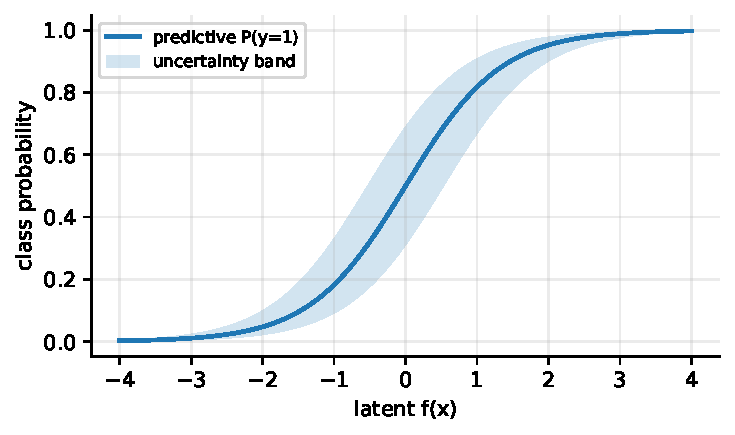
\includegraphics[width=0.9\textwidth]{gal_gpclass}
\caption{Gaussian-process classification. The predictive class probability carries the function uncertainty, widening where data are sparse rather than only near the boundary.}
\label{fig:gal_gpclass}
\end{figure}

Squashing the latent posterior through the logistic link pulls the predictive probability toward one-half wherever the function is uncertain, so the model hedges where it lacks data.


\section*{Choosing and averaging models}

\paragraph{Bayesian model averaging.}
Rather than select a single model, one averages predictions over models weighted by their posterior
probabilities $\Pb(M_k\mid D)\propto\Pb(D\mid M_k)\Pb(M_k)$, giving the predictive
$\sum_k\Pb(M_k\mid D)\,p(y_{\mathrm{new}}\mid D,M_k)$. Averaging improves the log-loss over any single
model chosen in advance, on average under the mixture's own predictive law, because it hedges model uncertainty rather than pretending it away, and it is the
model-space version of the mixture predictor.

\begin{figure}[H]
\centering
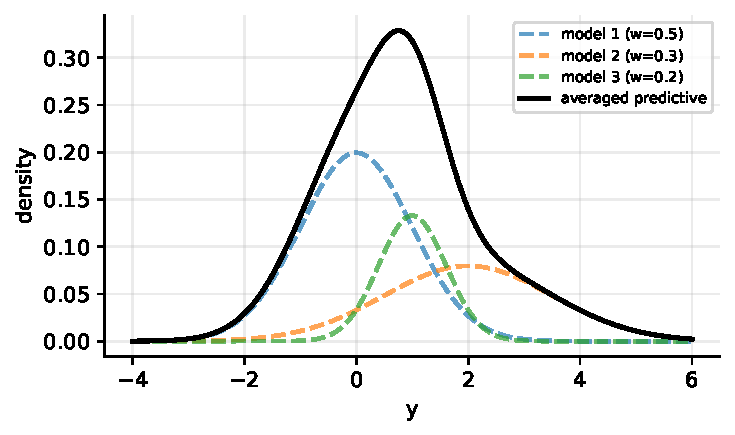
\includegraphics[width=0.9\textwidth]{gal_bma}
\caption{Bayesian model averaging. The predictive is a posterior-weighted mixture over models, which hedges model uncertainty and improves log-loss on average over any single choice.}
\label{fig:gal_bma}
\end{figure}


\paragraph{Optimal experimental design.}
Choosing the experiment $\mathcal E$ that maximizes the expected information $I(\mathcal E)=\E_y\,
\D{\pi(\cdot\mid y)}{\pi}$ is Lindley's criterion (Lindley, 1956), the mutual information between the
parameter and the data the experiment would yield. Design is prospective learning: one picks the question
whose answer is expected to move the posterior the most, and for a linear-Gaussian model this recovers the
classical D-optimality criterion.

\begin{figure}[H]
\centering
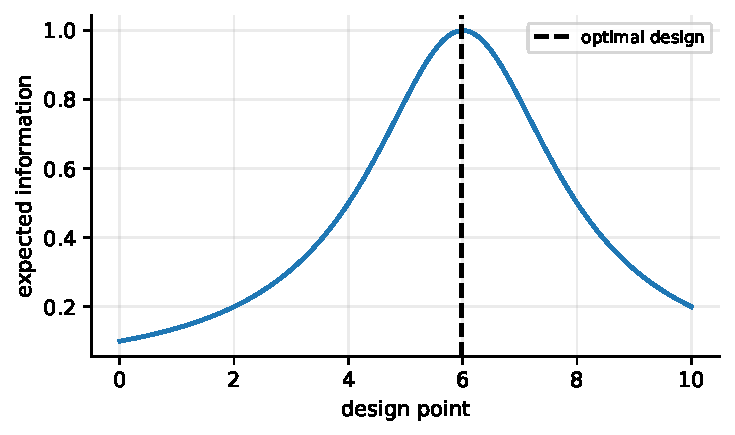
\includegraphics[width=0.9\textwidth]{gal_design}
\caption{Optimal design. Choosing the experiment that maximizes expected information (Lindley, 1956) picks the design point whose answer is expected to move the posterior most.}
\label{fig:gal_design}
\end{figure}

For a linear-Gaussian model the expected information depends on the design matrix alone, so the optimal experiment can be chosen before a single datum is collected.


\section*{Decisions and stopping}

\paragraph{The secretary problem.}
Interviewing candidates in random order and deciding irrevocably on each, the Bayes-optimal rule rejects
the first $n/e$ candidates and then hires the next one better than all seen so far, succeeding with
probability about $1/e\approx0.37$. Optimal stopping is sequential Bayesian decision: the posterior that
the current candidate is best is weighed against the option value of waiting.

\begin{figure}[H]
\centering
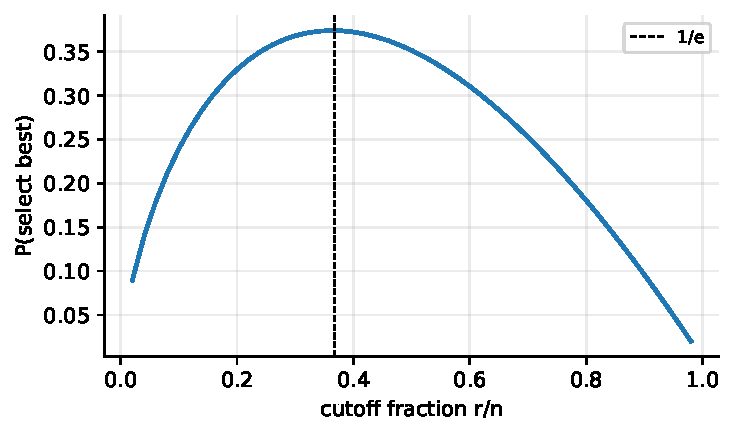
\includegraphics[width=0.9\textwidth]{gal_secretary}
\caption{Optimal stopping. The probability of selecting the best candidate peaks when the first $1/e$ of applicants are rejected out of hand and the next record is then hired.}
\label{fig:gal_secretary}
\end{figure}

For $n=100$ the rule rejects the first thirty-seven applicants and then hires the first later one who beats them all, selecting the very best about thirty-seven percent of the time; the curve is nearly flat at its peak, so the exact cutoff barely matters.


\paragraph{Gittins indices and the price of information.}
For a Bayesian bandit with independent arms and geometric discounting, the optimal policy attaches to each arm a scalar Gittins
index (Gittins, 1979), the retirement wage that makes pulling the arm and stopping indifferent, and plays the arm of
highest index. The index prices exploration exactly: an arm with an uncertain but promising posterior earns
an information bonus above its posterior mean, which is what Thompson sampling approximates by
randomization.

\begin{figure}[H]
\centering
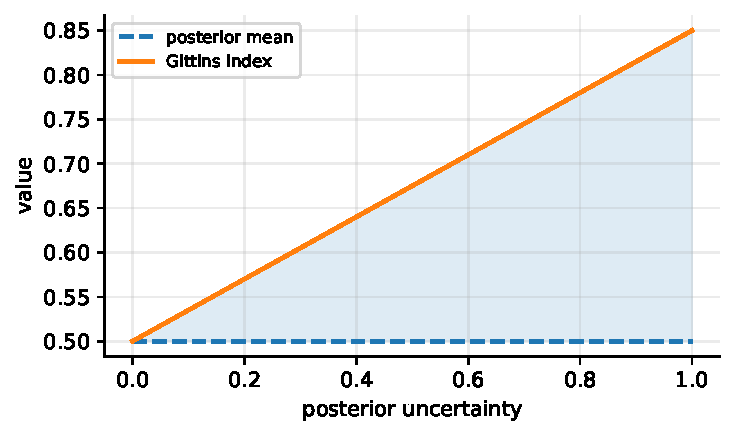
\includegraphics[width=0.9\textwidth]{gal_bandit}
\caption{The price of information. The Gittins index adds an exploration bonus above an arm's posterior mean that grows with its uncertainty, which randomized Thompson sampling mimics.}
\label{fig:gal_bandit}
\end{figure}


\section*{Estimation classics and computation}

\paragraph{Good--Turing and the unseen.}
Estimating the total probability of species not yet observed by the fraction of the sample seen exactly
once, $\Pb(\text{new})\approx N_1/n$, is a smoothing of the multinomial that behaves like a nonparametric
Bayesian estimate under a Pitman--Yor prior, the power-law extension of the Dirichlet process. It answers the question the raw frequencies cannot:
how much probability to reserve for what has not yet appeared. For large $n$ the Bayesian estimate of the probability of a new species under the Pitman--Yor process (Pitman and Yor, 1997) is asymptotically a smoothed Good--Turing estimate (Favaro, Nipoti and Teh, 2016).

\begin{figure}[H]
\centering
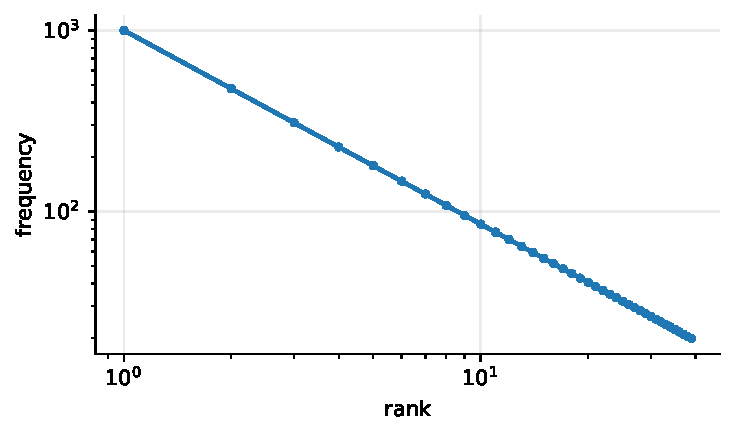
\includegraphics[width=0.9\textwidth]{gal_goodturing}
\caption{Frequency of frequencies. Heavy-tailed counts leave many rare types, and the mass to reserve for the unseen is estimated from the number of singletons.}
\label{fig:gal_goodturing}
\end{figure}

If a thousand-word sample has three hundred words appearing exactly once, roughly thirty percent of the next word's probability should be held back for words not yet seen.


\paragraph{The Bayesian bootstrap.}
Placing the improper $\mathrm{Dir}(0,\dots,0)$ prior on the weights of the observed sample and drawing them from the resulting
$\mathrm{Dir}(1,\dots,1)$ gives a posterior over the empirical distribution, and any functional
inherits a posterior by reweighting. Rubin's Bayesian bootstrap is nonparametric posterior inference with
no parametric model at all, the resampling face of the Dirichlet-process predictive.

\begin{figure}[H]
\centering
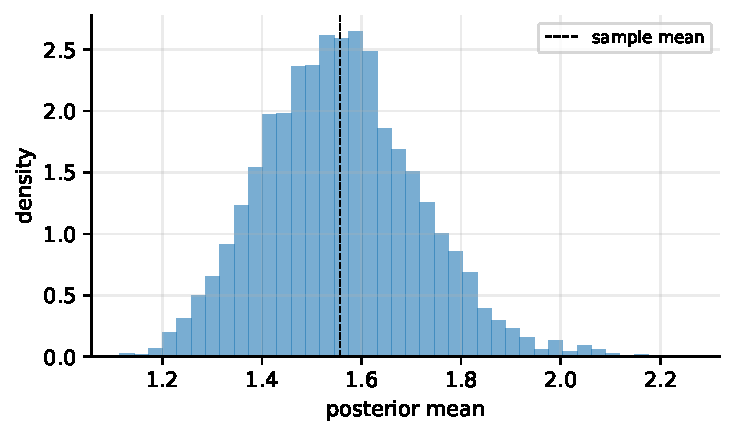
\includegraphics[width=0.9\textwidth]{gal_bootstrap}
\caption{The Bayesian bootstrap. Dirichlet weights on the sample induce a posterior over any functional; shown is the posterior of the mean, centered at the sample mean.}
\label{fig:gal_bootstrap}
\end{figure}

The Dirichlet-weighted means average to the sample mean, and their spread approximates the sampling distribution, giving interval statements with no asymptotic appeal.


\paragraph{The Laplace approximation.}
Approximating a posterior by the Gaussian $\N(\hat\theta,(n\bar j)^{-1})$ at its mode, with $\bar j$ the
average observed information, turns any smooth posterior into a tractable one and its normalizing constant
into the evidence to leading order. It is the workhorse behind BIC, the integrated nested Laplace
approximation, and the Occam factor, and it is exact in the large-sample limit by Bernstein--von Mises.



\begin{figure}[H]
\centering
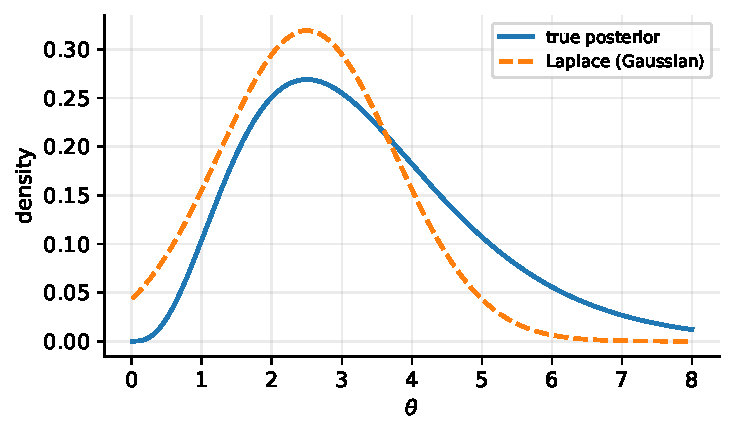
\includegraphics[width=0.9\textwidth]{gal_laplace}
\caption{The Laplace approximation. A Gaussian centered at the mode with the observed-information curvature matches a smooth posterior, exactly so in the large-sample limit.}
\label{fig:gal_laplace}
\end{figure}

For a $\mathrm{Gamma}(4,1.2)$ posterior the mode sits at $2.5$ and the observed-information curvature there gives a Gaussian of standard deviation about $1.44$; the fit is good in the body and understates the right tail, an error that shrinks as the shape parameter grows.
\paragraph{Importance sampling as weighted learning.}
Estimating a posterior expectation by drawing from a proposal $q$ and reweighting by
$w(\theta)\propto\pi(\theta)p(D\mid\theta)/q(\theta)$ is Monte Carlo Bayes, and the self-normalized version
needs only unnormalized densities. The effective sample size $(\sum w)^2/\sum w^2$ measures how much the
proposal has learned about the posterior, and it collapses when the proposal misses the mass, the
diagnostic every practitioner watches.

\begin{figure}[H]
\centering
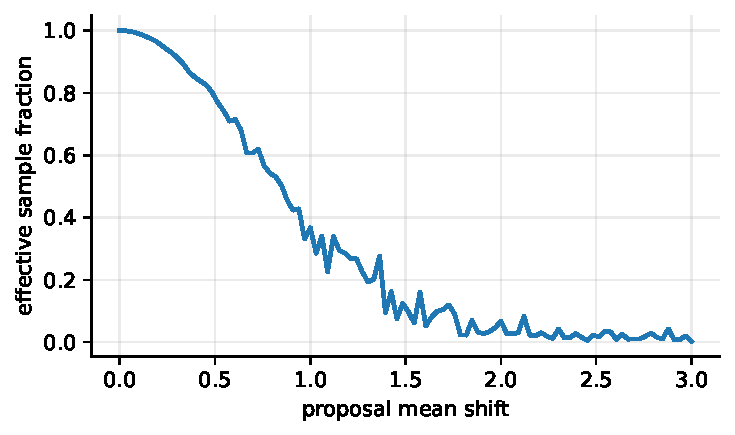
\includegraphics[width=0.9\textwidth]{gal_importance}
\caption{Importance sampling. The effective sample fraction collapses as the proposal drifts from the target, the diagnostic that warns when a proposal has learned little.}
\label{fig:gal_importance}
\end{figure}

A proposal shifted one standard deviation from the target already more than halves the effective sample, and by three it leaves almost all weight on a handful of draws, the variance exploding.



\section*{Regression, ranking, and calibration}

\paragraph{Probit and logistic regression by augmentation.}
Binary regression becomes conjugate through one latent variable. For the probit link, Albert and Chib (1993)
draw a latent Gaussian $z_i\sim\N(x_i^\top\beta,1)$ truncated to the sign of $y_i$, after which
$\beta\mid z$ is an ordinary Gaussian regression draw; for the logistic link the P\'olya--Gamma weight
plays the same role. Classification is thus Gaussian learning conducted on a latent utility, and the
posterior on $\beta$ carries the uncertainty a point estimate discards.

\paragraph{Learning strengths from comparisons.}
The Bradley--Terry model gives each competitor a strength $\theta_i$ and sets $\Pb(i\ \text{beats}\ j)=
\sigma(\theta_i-\theta_j)$ with $\sigma$ the logistic function; a Gaussian prior on the strengths and P\'olya--Gamma augmentation make the
posterior a sequence of conjugate updates from observed wins and losses. Learning who is better from
pairwise outcomes is logistic regression on difference vectors, and it is the engine behind chess ratings and preference learning.

\begin{figure}[H]
\centering
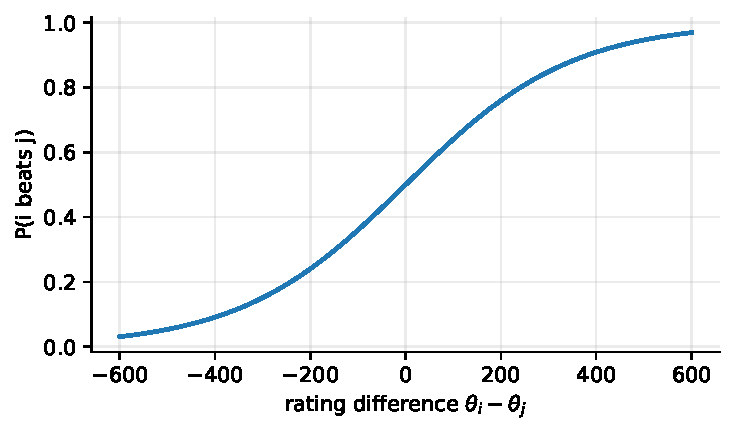
\includegraphics[width=0.9\textwidth]{gal_bradleyterry}
\caption{Learning from comparisons. The Bradley--Terry win probability is a logistic function of the rating difference, so paired-comparison learning is logistic regression.}
\label{fig:gal_bradleyterry}
\end{figure}

A four-hundred-point gap is about a ninety-percent win probability, the scale chess adopted, and the maximum-likelihood strengths are a logistic regression on the win-loss matrix.

\paragraph{Elo and TrueSkill as sequential Bayes.}
Updating a player's rating after each game (Elo, 1978) by a step proportional to the surprise, actual minus expected
score, is the online, Gaussian-approximate version of Bradley--Terry learning; TrueSkill carries a full
Gaussian posterior per player and updates it by message passing. A rating system is a Kalman filter on
skill, and its uncertainty is why new players' ratings move fast and veterans' move slowly.

\begin{figure}[H]
\centering
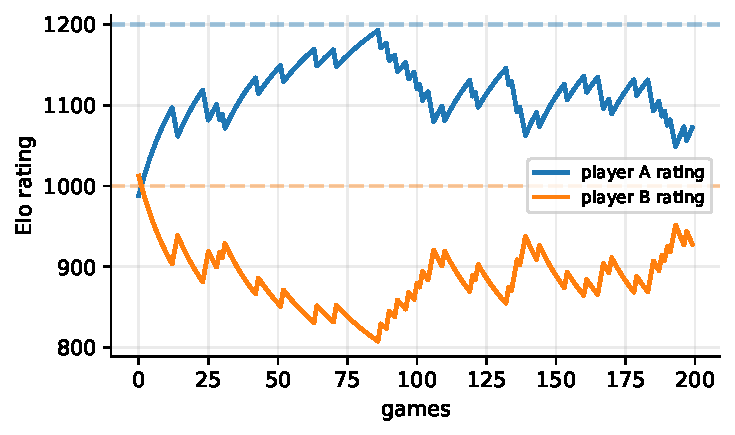
\includegraphics[width=0.9\textwidth]{gal_elo}
\caption{Sequential rating. Elo updates are online Gaussian Bradley--Terry learning; ratings drift toward the players' true skills, fast at first and then slowly.}
\label{fig:gal_elo}
\end{figure}

With a step size of twenty-four a single upset moves a rating by at most twenty-four points, so ratings follow genuine skill over tens of games while averaging out the noise in any one result.


\paragraph{Calibration of predicted probabilities.}
A classifier's raw scores are recalibrated by fitting a small monotone map, Platt scaling a logistic and
beta calibration a two-parameter beta, so that among cases predicted at probability $q$ about a fraction
$q$ are positive. Calibration is a one-dimensional Bayesian regression of outcomes on scores, and it is
the coverage side of the coverage-versus-coherence axis of the opening chapter.

\begin{figure}[H]
\centering
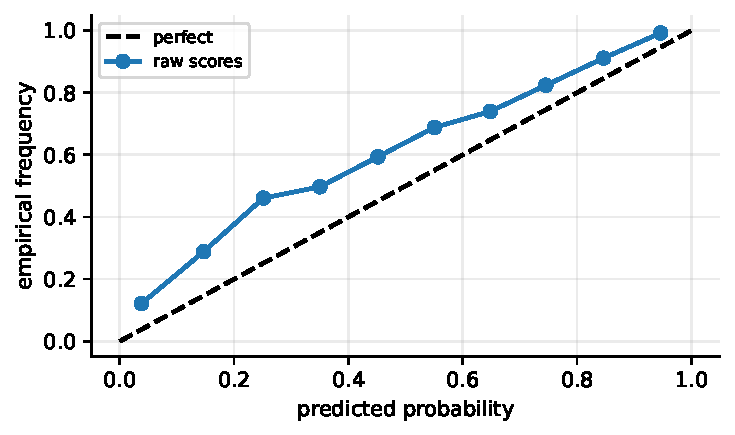
\includegraphics[width=0.9\textwidth]{gal_calibration}
\caption{Calibration. A reliability diagram plots empirical frequency against predicted probability; departures from the diagonal are the miscalibration a monotone recalibration removes.}
\label{fig:gal_calibration}
\end{figure}

A model can be sharp yet miscalibrated: confident predictions right only eighty percent of the time bow the reliability curve below the diagonal, and one monotone fit restores it without disturbing the ranking.


\paragraph{Conformal prediction and finite-sample coverage.}
Ranking a new point's nonconformity score among the calibration scores and reporting the set of labels
whose rank is not extreme yields, under exchangeability alone, a prediction set with finite-sample
coverage at least $1-\alpha$. No model is assumed correct; the guarantee is distribution-free calibration, and it
coincides asymptotically with a Bayesian predictive interval when the model is correct and the nonconformity score is the Bayesian
predictive density.

\begin{figure}[H]
\centering
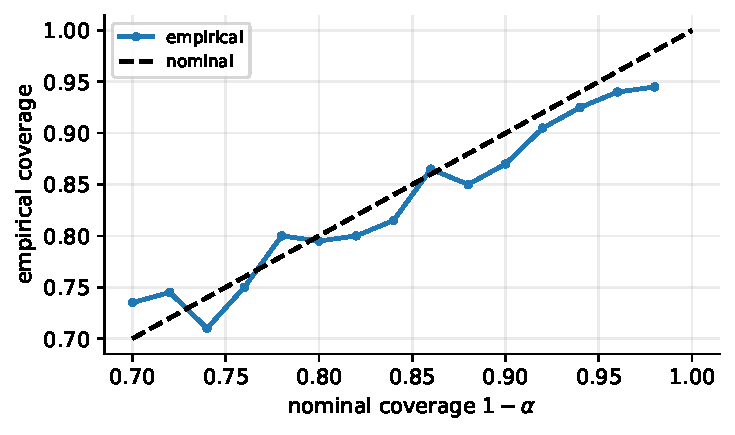
\includegraphics[width=0.9\textwidth]{gal_conformal}
\caption{Conformal prediction. Ranking a new score among the calibration scores gives finite-sample coverage that tracks the nominal level under exchangeability alone.}
\label{fig:gal_conformal}
\end{figure}

The guarantee holds for any nonconformity score and any sample size, trading the sharpness a correct model would add for coverage that survives misspecification.


\section*{Hierarchies, structure, and priors}

\paragraph{Random-effects meta-analysis.}
Combining study estimates $\hat\theta_j$ with standard errors $s_j$ under $\theta_j\sim\N(\mu,\tau^2)$
gives each study the shrunk estimate $(1-B_j)\hat\theta_j+B_j\mu$ with $B_j=s_j^2/(s_j^2+\tau^2)$, and the
data estimate $\tau^2$, hence how much to pool. Meta-analysis is the eight-schools shrinkage applied to a
literature, and partial pooling is why a small, noisy study is pulled hardest toward the consensus.

\begin{figure}[H]
\centering
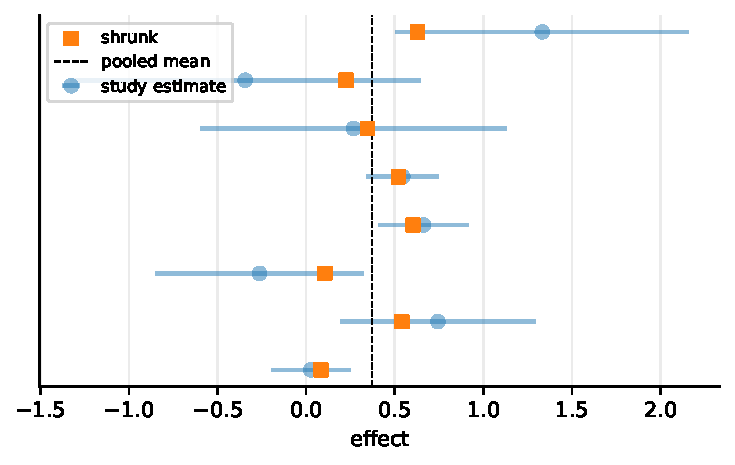
\includegraphics[width=0.9\textwidth]{gal_meta}
\caption{Partial pooling. Random-effects meta-analysis shrinks each study estimate toward the pooled mean by a weight set by its noise, most for the least precise studies.}
\label{fig:gal_meta}
\end{figure}

A study with standard error $0.4$ against a between-study spread $\tau=0.25$ carries weight $B\approx0.72$ toward the pooled mean, so it is shrunk almost three-quarters of the way, whereas a precise study with standard error $0.1$ hardly moves.


\paragraph{Probabilistic principal component analysis.}
Modeling $y=Wz+\varepsilon$ with latent $z\sim\N(0,I)$ and isotropic noise makes PCA a Gaussian latent
factor model whose maximum-likelihood loading spans the top principal subspace, and a prior on $W$ turns
it into Bayesian factor analysis with automatic dimensionality selection. Dimension reduction is Gaussian
learning of a low-rank covariance, with the noise floor setting how many directions survive.

\begin{figure}[H]
\centering
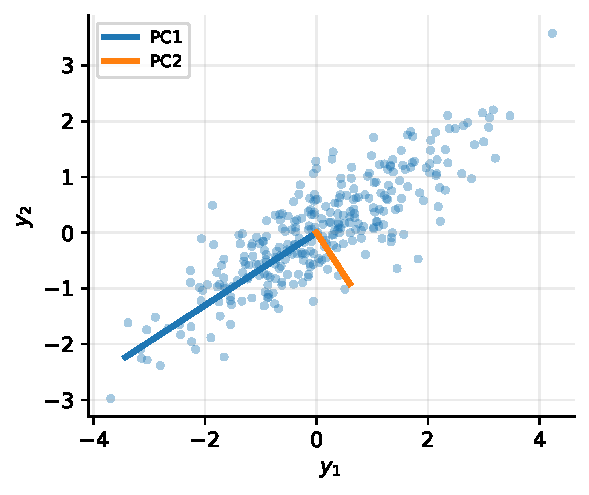
\includegraphics[width=0.9\textwidth]{gal_pca}
\caption{Probabilistic PCA. A Gaussian latent-factor model learns the principal axes as the directions of greatest variance, the noise floor setting the retained dimension.}
\label{fig:gal_pca}
\end{figure}

Keeping the components above the noise floor recovers the signal subspace, and the marginal likelihood of the isotropic-noise model peaks at the true rank, an automatic stopping rule.


\paragraph{Jeffreys' prior from information.}
Requiring a prior that is a function of the Fisher information to be invariant to smooth reparametrization forces $\pi(\theta)\propto\lvert\mathcal
I(\theta)\rvert^{1/2}$, Jeffreys' rule, the density that is flat in the natural distance of the model.
It is the prior that asymptotically maximizes the expected information an experiment provides in the one-parameter case
and so is the reference prior, closing the loop with Lindley's design criterion and the Schwarz penalty of
Section~\ref{ch:risk}.

\begin{figure}[H]
\centering
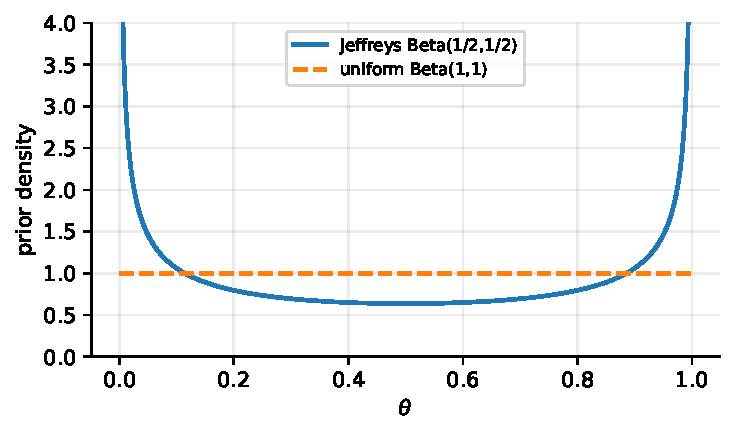
\includegraphics[width=0.9\textwidth]{gal_jeffreys}
\caption{Jeffreys' prior. The invariant reference prior for a binomial is the arcsine density $\mathrm{Beta}(\tfrac12,\tfrac12)$, flat in the model's natural distance rather than in $\theta$.}
\label{fig:gal_jeffreys}
\end{figure}


\section*{Processes and computation}

\paragraph{Learning an arrival rate.}
For events arriving as a Poisson process with rate $\lambda$, observing $k$ events in time $T$ under a
$\mathrm{Gamma}(a,b)$ prior gives the posterior $\mathrm{Gamma}(a+k,b+T)$, and letting the rate itself
vary as a Gaussian process yields a Cox process. Learning how often something happens is gamma-Poisson
updating in continuous time, and the predictive interarrival law is again heavy-tailed.

\begin{figure}[H]
\centering
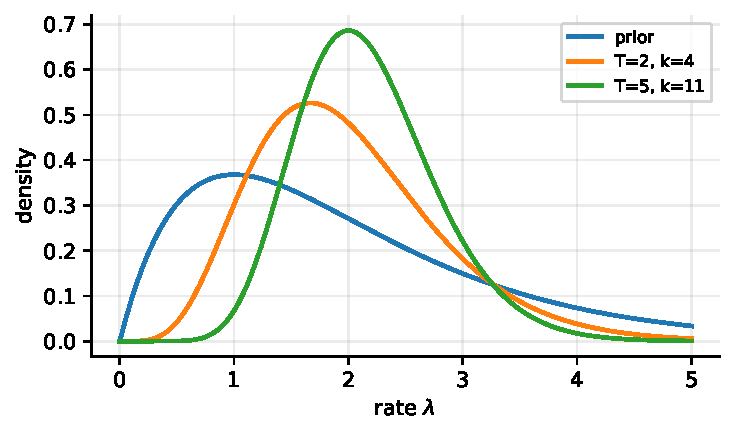
\includegraphics[width=0.9\textwidth]{gal_arrival}
\caption{Learning an arrival rate. Gamma-Poisson updating in continuous time sharpens the posterior on the rate as events accrue over a longer window.}
\label{fig:gal_arrival}
\end{figure}

Eleven events in five time units under a $\mathrm{Gamma}(2,1)$ prior give posterior $\mathrm{Gamma}(13,6)$, mean rate $2.17$ and standard deviation $0.60$, sharpening as the window lengthens.


\paragraph{Bayesian quadrature.}
Placing a Gaussian-process prior on an integrand and conditioning on its evaluations turns numerical
integration into posterior inference: the estimate is the posterior mean of the integral and the error
bar is its posterior standard deviation. Probabilistic numerics treats computation as learning, and it
spends evaluations where the integrand is most uncertain rather than on a fixed grid.

\begin{figure}[H]
\centering
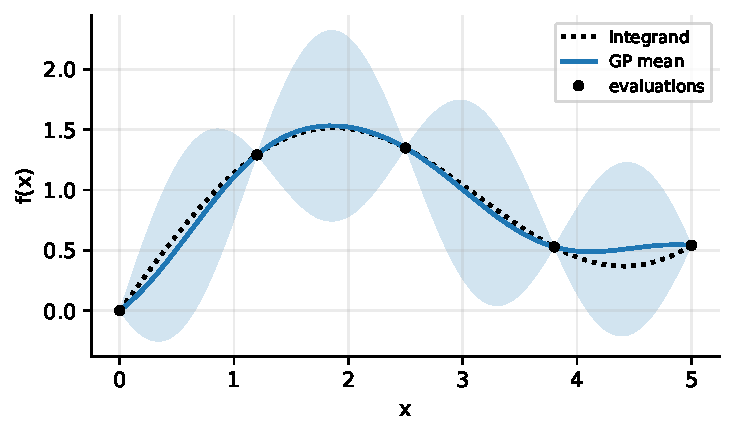
\includegraphics[width=0.9\textwidth]{gal_quadrature}
\caption{Bayesian quadrature. A Gaussian-process prior on the integrand turns integration into inference, spending evaluations where the integrand is most uncertain.}
\label{fig:gal_quadrature}
\end{figure}


\paragraph{Stein's unbiased risk estimate.}
For a nearly arbitrary estimator $y+g(y)$ of a Gaussian mean observed as $y\sim\N(\theta,I_n)$, Stein's identity gives an unbiased estimate of its
mean squared error from the data alone, $\mathrm{SURE}=n+\lVert g\rVert^2+2\nabla\!\cdot g$, so a tuning
parameter can be chosen by minimizing risk without a validation set. It is the frequentist twin of the
evidence, and it selects shrinkage in the regime where James--Stein operates.

\begin{figure}[H]
\centering
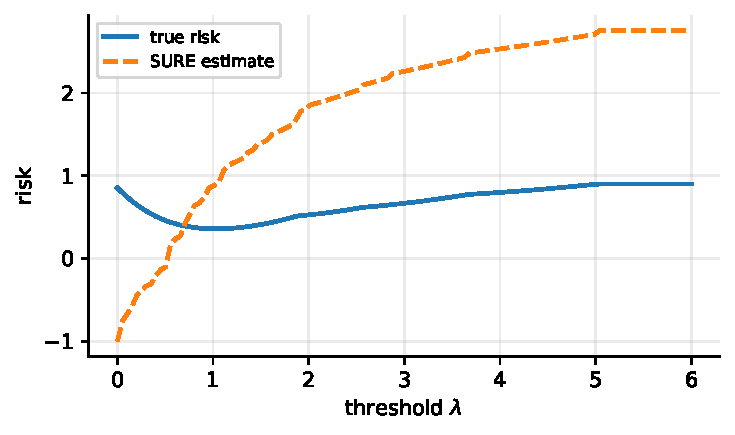
\includegraphics[width=0.9\textwidth]{gal_sure}
\caption{Stein's unbiased risk. SURE estimates the mean squared error of a thresholding rule from the data alone, so the threshold can be tuned without a validation set.}
\label{fig:gal_sure}
\end{figure}



\backmatter
\chapter*{References}
\addcontentsline{toc}{chapter}{References}
\markboth{REFERENCES}{REFERENCES}

\section*{Core source papers (this research program)}
\begin{enumerate}[leftmargin=2.2em]
\item Polson, N.\,G., and Zantedeschi, D. De Finetti + Sanov = Bayes: Forward and Inverse Sanov
in Bayesian Prediction. Revised Short Communication, \emph{Statistical Science} (STS2509 011);
arXiv:2509.13283 (2025a; revised 2026), whose versions~2 and~3 are titled De Finetti + Sanov = Bayes: Exchangeable Prediction under Moment Constraints. Earlier title: Gibbs Conditioning for Exchangeable Prediction under Moment
Constraints. Includes the Heath--Sudderth scalar-method-of-types merge (note of 14
July 2026).
\item Polson, N.\,G., and Zantedeschi, D. Bayesian Prediction under Moment Conditioning.
arXiv:2510.20742 (2025b; revised 2026).
\item Polson, N.\,G., and Zantedeschi, D. Entropy-Regularized Inference: A Predictive
Approach. arXiv:2512.21639 (2025c; revised 2026). Version~1 titled Rational Inattention: A
Bayesian Predictive Approach.
\item Polson, N.\,G., and Zantedeschi, D. Martingale Posterior Predictive Coherence: Hausdorff
Moment Hierarchy. arXiv:2603.00661 (2026a).
\item Polson, N.\,G., and Zantedeschi, D. Bayes with No Shame: Admissibility Geometries of
Predictive Inference. arXiv:2603.05335 (2026b).
\item Polson, N.\,G., and Zantedeschi, D. E-Values, Bayes Risk, Dual Role of Markov's
Inequality. arXiv:2604.00337 (2026c).
\item Polson, N.\,G., Sokolov, V., and Zantedeschi, D. Bayes, E-values, and Testing.
arXiv:2602.04146 (2026a).
\item Datta, J., Polson, N.\,G., Sokolov, V., and Zantedeschi, D. A New Look at Bayesian
Testing. arXiv:2602.11132 (2026).
\item Polson, N.\,G., Sokolov, V., and Zantedeschi, D. Bayes Risk for Goodness of Fit
Tests. arXiv:2602.15297 (2026b).
\item Polson, N.\,G., Sokolov, V., and Zantedeschi, D. Horseshoe Priors and MDP.
arXiv:2604.01266 (2026c).
\item Polson, N.\,G., and Zantedeschi, D. Nonparametric Predictive Bayes Risk. Working paper (2026i). Submitted to \emph{Journal of the American Statistical Association}.
\item Polson, N.\,G., Sokolov, V., and Zantedeschi, D. Minimum Description Length, Bayesian Evidence, and the Information-Theoretic View of Model Selection. Working paper (2026d).
\item Polson, N.\,G., and Sokolov, V. Kolmogorov on Cybernetics. Working paper (2026a).
\item Polson, N.\,G., and Zantedeschi, D. Maximum Entropy Algorithms for Predictive Rules:
Blahut--Arimoto, Conditional Limits, and Iterative Scaling. Working paper (2026d).
\item Polson, N.\,G., and Zantedeschi, D. When Is Bayes Gaussian? Curvature of the Rate
Function, from Bernstein--von Mises to Ghosh. Working notes (2026e).
\item Polson, N.\,G., Sokolov, V., and Zantedeschi, D. Bayes Factors and Moderate
Deviations in Genome-Wide Screening. SSRN 7167078
(2026e), posted under the title Bayes Factors and Moderate Deviations in High-Throughput Screening.
\item Polson, N.\,G., and Zantedeschi, D. Federated Learning, de Finetti, and
Sanov. Working paper (2026f). Source of Section~\ref{ch:federated}.
\item Polson, N.\,G., and Zantedeschi, D. Bayesian Asymptotics: Merging, Martingales, and Moderate Deviations. SSRN 7013738 (2026j). Submitted to \emph{International Statistical Review}.
\item Polson, N.\,G., Sokolov, V., and Zantedeschi, D. Linear Bayes Methods for Prediction-Powered Inference. SSRN 6744239 (2026f).
\item Polson, N.\,G., Sokolov, V., and Zantedeschi, D. Ordered Empirical Bayes: A Default Regularizer for Score-Based Generative Models. SSRN 7167039 (2026g).
\item Polson, N.\,G., Sokolov, V., and Zantedeschi, D. A Critique of Martingale Posteriors. Working paper (2026).
\item Polson, N.\,G., Sokolov, V., and Zantedeschi, D. E-Values and Sanov's Theorem. Working paper (2026).
\item Polson, N.\,G., Sokolov, V., and Zantedeschi, D. Generative Bayesian Computation: A Measure-Theoretic Framework for Utility-Based Causal Inference. Working paper (2026).
\item Datta, J., Polson, N.\,G., and Sokolov, V. Bayesian Global-Local Regularization. arXiv:2512.13992 (2025).
\item Polson, N.\,G., and Sokolov, V. Bayesian Double Descent. arXiv:2507.07338 (2025).
\end{enumerate}
\noindent Companion (in preparation): Polson, N.\,G., and Zantedeschi, D. Deviation Rates,
Conditioning, and Exact Convergence: From Hoeffding's o(n) to the Brandeis Dice (2026h).

\section*{Selected references, with the Ganesh papers}
\begin{enumerate}[leftmargin=2.2em]
\item Billingsley, P. \emph{Probability and Measure}, 3rd ed. (1995). [Helly and Helly--Bray.]
\item Carvalho, C.\,M., Polson, N.\,G., and Scott, J.\,G. The horseshoe estimator for sparse signals.
\emph{Biometrika} \textbf{97}, 465--480 (2010).
\item Csisz\'ar, I. I-divergence geometry of probability distributions and minimization problems.
\emph{Annals of Probability} \textbf{3}, 146--158 (1975).
\item Csisz\'ar, I. Sanov property, generalized I-projection and a conditional limit theorem. \emph{Annals of Probability} \textbf{12}, 768--793 (1984).
\item de Finetti, B. La pr\'evision: ses lois logiques, ses sources subjectives. \emph{Annales de l'Institut Henri Poincar\'e} \textbf{7}, 1--68 (1937).
\item Diaconis, P., and Freedman, D.\,A. Finite exchangeable sequences. \emph{Annals of Probability} \textbf{8}, 745--764 (1980a).
\item Diaconis, P., and Freedman, D.\,A. On the consistency of Bayes estimates. \emph{Annals of Statistics} \textbf{14}, 1--26 (1986).
\item Diaconis, P., and Freedman, D.\,A. Conditional limit theorems for exponential families and
finite versions of de Finetti's theorem. \emph{Journal of Theoretical Probability} \textbf{1}, 381--410 (1988).
\item Eichelsbacher, P., and Ganesh, A. Moderate deviations for Bayes posteriors. \emph{Scandinavian Journal of Statistics} \textbf{29}, 153--167 (2002a).
\item Eichelsbacher, P., and Ganesh, A. Bayesian inference for Markov chains. \emph{Journal of Applied Probability} \textbf{39}, 91--99 (2002b).
\item Fan, J., Hall, P., and Yao, Q. To how many simultaneous hypothesis tests can normal, Student's $t$ or
bootstrap calibration be applied? \emph{Journal of the American Statistical Association} \textbf{102}, 1282--1288 (2007).
\item Ganesh, A., and O'Connell, N. An inverse of Sanov's theorem. In \emph{Proceedings of the 1998 IEEE International Symposium on Information Theory}, p.\ 413 (1998).
\item Ganesh, A., and O'Connell, N. An inverse of Sanov's theorem. \emph{Statistics \&
Probability Letters} \textbf{42}, 201--206 (1999).
\item Ganesh, A., and O'Connell, N. A large-deviation principle for Dirichlet posteriors.
\emph{Bernoulli} \textbf{6}, 1021--1034 (2000).
\item Heath, D., and Sudderth, W. De Finetti's theorem on exchangeable variables. \emph{The American
Statistician} \textbf{30}, 188--189 (1976).
\item Jaynes, E.\,T. Information theory and statistical mechanics. \emph{Physical Review} \textbf{106}, 620--630 (1957).
\item Jaynes, E.\,T. Information theory and statistical mechanics (notes by the lecturer). In \emph{Statistical Physics} \textbf{3} (Brandeis Summer Institute 1962), Benjamin, New York, 181--218 (1963).
\item Jaynes, E.\,T. On the rationale of maximum-entropy methods. \emph{Proceedings of the IEEE} \textbf{70}, 939--952 (1982).
\item Jeffreys, H. Further significance tests. \emph{Proceedings of the Cambridge Philosophical Society} \textbf{32}, 416--445 (1936).
\item Jeffreys, H. \emph{Theory of Probability}, 3rd ed. (1961).
\item Kleijn, B.\,J.\,K., and van der Vaart, A.\,W. The Bernstein--von Mises theorem under
misspecification. \emph{Electronic Journal of Statistics} \textbf{6}, 354--381 (2012).
\item Larsson, M., Ramdas, A., and Ruf, J. The numeraire e-variable and reverse information projection. \emph{Annals of Statistics} \textbf{53}, 1015--1043 (2025).
\item L\'eonard, C., and Najim, J. An extension of Sanov's theorem: application to the Gibbs
conditioning principle. \emph{Bernoulli} \textbf{8}, 721--743 (2002).
\item Lorden, G. On excess over the boundary. \emph{Annals of Mathematical Statistics} \textbf{41}, 520--527 (1970).
\item Macci, C., and Piccioni, M. An inverse Sanov theorem for exponential families.
\emph{Journal of Statistical Planning and Inference} \textbf{224}, 54--68 (2023).
\item Rubin, H., and Sethuraman, J. Probabilities of moderate deviations. \emph{Sankhya A} \textbf{27}, 325--346 (1965a).
\item Rubin, H., and Sethuraman, J. Bayes risk efficiency. \emph{Sankhya A} \textbf{27}, 347--356 (1965b).
\item Sanov, I.\,N. On the probability of large deviations of random variables. \emph{Matematicheskii Sbornik} \textbf{42}, 11--44 (1957).
\item Shore, J.\,E., and Johnson, R.\,W. Axiomatic derivation of the principle of maximum entropy and the principle of minimum cross-entropy. \emph{IEEE Transactions on Information Theory} \textbf{26}, 26--37 (1980).
\item Stern, H., and Cover, T.\,M. Maximum entropy and the lottery. \emph{Journal of the American Statistical Association} \textbf{84}, 980--985 (1989).
\item van Campenhout, J.\,M., and Cover, T.\,M. Maximum entropy and conditional probability. \emph{IEEE Transactions on Information Theory} \textbf{27}, 483--489 (1981).
\item Ville, J. \emph{\'Etude critique de la notion de collectif}. Monographies des Probabilit\'es, Fascicule III, Gauthier-Villars, Paris (1939).
\item Wakefield, J. Bayes factors for genome-wide association studies. \emph{Genetic Epidemiology} \textbf{33}, 79--86 (2009).
\end{enumerate}

\section*{Algorithms, computation, and federated inference}
\begin{enumerate}[leftmargin=2.2em]
\item Aldous, D.\,J. Representations for partially exchangeable arrays of random variables. \emph{Journal
of Multivariate Analysis} \textbf{11}, 581--598 (1981).
\item Amari, S., and Nagaoka, H. \emph{Methods of Information Geometry} (2000).
\item Arimoto, S. An algorithm for computing the capacity of arbitrary discrete memoryless channels.
\emph{IEEE Transactions on Information Theory} \textbf{18}, 14--20 (1972).
\item Bauschke, H.\,H., and Lewis, A.\,S. Dykstra's algorithm with Bregman projections: a
convergence proof. \emph{Optimization} \textbf{48}, 409--427 (2000).
\item Beck, A., and Teboulle, M. Mirror descent and nonlinear projected subgradient methods for
convex optimization. \emph{Operations Research Letters} \textbf{31}, 167--175 (2003).
\item Blahut, R.\,E. Computation of channel capacity and rate-distortion functions. \emph{IEEE Transactions on Information Theory} \textbf{18}, 460--473 (1972).
\item B\"ohning, D. Multinomial logistic regression algorithm. \emph{Annals of the Institute of Statistical Mathematics} \textbf{44}, 197--200 (1992).
\item B\"ohning, D., and Lindsay, B.\,G. Monotonicity of quadratic-approximation algorithms. \emph{Annals of the Institute of Statistical Mathematics} \textbf{40}, 641--663 (1988).
\item Bouchard, G. Efficient bounds for the softmax function and applications to approximate
inference in hybrid models. NIPS 2007 workshop on approximate Bayesian inference (2007).
\item Bregman, L.\,M. The relaxation method of finding the common point of convex sets. \emph{USSR Computational Mathematics and Mathematical Physics} \textbf{7}, 200--217 (1967).
\item Censor, Y., and Reich, S. The Dykstra algorithm with Bregman projections. \emph{Communications in Applied Analysis} \textbf{2}, 407--419 (1998).
\item Censor, Y., and Zenios, S.\,A. Proximal minimization algorithm with $D$-functions. \emph{Journal of Optimization Theory and Applications} \textbf{73}, 451--464 (1992).
\item Chen, G., and Teboulle, M. Convergence analysis of a proximal-like minimization algorithm
using Bregman functions. \emph{SIAM Journal on Optimization} \textbf{3}, 538--543 (1993).
\item Chen, X.-H., Dempster, A.\,P., and Liu, J.\,S. Weighted finite population sampling to maximize
entropy. \emph{Biometrika} \textbf{81}, 457--469 (1994).
\item Chentsov, N.\,N. \emph{Statistical Decision Rules and Optimal Inference}. Translations of Mathematical Monographs 53, American Mathematical Society (1982).
\item Cover, T.\,M., and Thomas, J.\,A. \emph{Elements of Information Theory}, 2nd ed. (2006).
\item Csisz\'ar, I., and Tusn\'ady, G. Information geometry and alternating minimization procedures.
\emph{Statistics and Decisions}, Supplement Issue \textbf{1}, 205--237 (1984).
\item Cuturi, M. Sinkhorn distances: lightspeed computation of optimal transport. In \emph{Advances in Neural Information Processing Systems} \textbf{26}, 2292--2300 (2013).
\item Darroch, J.\,N., and Ratcliff, D. Generalized iterative scaling for log-linear models. \emph{Annals of Mathematical Statistics} \textbf{43}, 1470--1480 (1972).
\item Della Pietra, S., Della Pietra, V., and Lafferty, J. Inducing features of random fields. \emph{IEEE Transactions on Pattern Analysis and Machine Intelligence} \textbf{19}, 380--393 (1997).
\item Deming, W.\,E., and Stephan, F.\,F. On a least squares adjustment of a sampled frequency table.
\emph{Annals of Mathematical Statistics} \textbf{11}, 427--444 (1940).
\item Donsker, M.\,D., and Varadhan, S.\,R.\,S. Asymptotic evaluation of certain Markov process
expectations for large time, IV. \emph{Communications on Pure and Applied Mathematics} \textbf{36}, 183--212 (1983).
\item Dykstra, R.\,L. An iterative procedure for obtaining I-projections onto the intersection of
convex sets. \emph{Annals of Probability} \textbf{13}, 975--984 (1985).
\item Eckstein, J. Nonlinear proximal point algorithms using Bregman functions. \emph{Mathematics of Operations Research} \textbf{18}, 202--226 (1993).
\item Fienberg, S.\,E. An iterative procedure for estimation in contingency tables. \emph{Annals of Mathematical Statistics} \textbf{41}, 907--917 (1970).
\item Fu, J.\,C., and Kass, R.\,E. The exponential rates of convergence of posterior distributions.
\emph{Annals of the Institute of Statistical Mathematics} \textbf{40}, 683--691 (1988).
\item Hoover, D.\,N. Relations on Probability Spaces and Arrays of Random Variables. Preprint, Institute for Advanced Study, Princeton (1979).
\item Hunter, D.\,R., and Lange, K. A tutorial on MM algorithms. \emph{The American Statistician} \textbf{58}, 30--37 (2004).
\item Jaakkola, T.\,S., and Jordan, M.\,I. Bayesian parameter estimation via variational methods.
\emph{Statistics and Computing} \textbf{10}, 25--37 (2000).
\item Kitamura, Y., and Stutzer, M. An information-theoretic alternative to generalized method of
moments estimation. \emph{Econometrica} \textbf{65}, 861--874 (1997).
\item Kullback, S. \emph{Information Theory and Statistics} (1959).
\item Lange, K., Hunter, D.\,R., and Yang, I. Optimization transfer using surrogate objective
functions. \emph{Journal of Computational and Graphical Statistics} \textbf{9}, 1--20 (2000).
\item Ma\'ckowiak, B., Mat\v{e}jka, F., and Wiederholt, M. Rational inattention: a review. \emph{Journal of Economic Literature} \textbf{61}, 226--273 (2023).
\item Mat\v{e}jka, F., and McKay, A. Rational inattention to discrete choices. \emph{American Economic Review} \textbf{105}, 272--298 (2015).
\item McFadden, D. Conditional logit analysis of qualitative choice behavior. In \emph{Frontiers in Econometrics} (Zarembka, ed.), Academic Press, 105--142 (1974).
\item McMahan, H.\,B., Moore, E., Ramage, D., Hampson, S., and Ag\"uera y Arcas, B.
Communication-efficient learning of deep networks from decentralized data. \emph{Proceedings of the 20th International Conference on Artificial Intelligence and Statistics}, PMLR \textbf{54}, 1273--1282 (2017).
\item Mironov, I. R\'enyi differential privacy. In \emph{2017 IEEE 30th Computer Security Foundations Symposium}, 263--275 (2017).
\item Moreau, J.-J. Proximit\'e et dualit\'e dans un espace hilbertien. \emph{Bulletin de la Soci\'et\'e Math\'ematique de France} \textbf{93}, 273--299 (1965).
\item Nemirovski, A., and Yudin, D. \emph{Problem Complexity and Method Efficiency in Optimization} (1983).
\item Owen, A.\,B. \emph{Empirical Likelihood} (2001).
\item Parikh, N., and Boyd, S. Proximal algorithms. \emph{Foundations and Trends in Optimization} \textbf{1}, 127--239 (2014).
\item Peyr\'e, G., and Cuturi, M. Computational optimal transport. \emph{Foundations and Trends in Machine Learning} \textbf{11}, 355--607 (2019).
\item Polson, N.\,G., and Scott, J.\,G. Mixtures, envelopes and hierarchical duality. \emph{Journal of the Royal Statistical Society, Series B} \textbf{78}, 701--727 (2016).
\item Sims, C.\,A. Implications of rational inattention. \emph{Journal of Monetary Economics} \textbf{50}, 665--690 (2003).
\item Sims, C.\,A. Rational inattention: beyond the linear-quadratic case. \emph{American Economic Review} \textbf{96}, 158--163 (2006).
\item Sims, C.\,A. Rational inattention and monetary economics. In \emph{Handbook of Monetary Economics}, vol.\ \textbf{3}, Elsevier, 155--181 (2010).
\item Sinkhorn, R. A relationship between arbitrary positive matrices and doubly stochastic matrices.
\emph{Annals of Mathematical Statistics} \textbf{35}, 876--879 (1964).
\item Teboulle, M. Entropic proximal mappings with applications to nonlinear programming. \emph{Mathematics of Operations Research} \textbf{17}, 670--690 (1992).
\item van der Pas, S.\,L., Kleijn, B.\,J.\,K., and van der Vaart, A.\,W. The horseshoe estimator:
posterior concentration around nearly black vectors. \emph{Electronic Journal of Statistics} \textbf{8}, 2585--2618 (2014).
\item van der Pas, S.\,L., Salomond, J.-B., and Schmidt-Hieber, J. Conditions for posterior contraction in the sparse normal means problem. \emph{Electronic Journal of Statistics} \textbf{10}, 976--1000 (2016).
\item van der Pas, S.\,L., Szab\'o, B., and van der Vaart, A.\,W. Adaptive posterior contraction
rates for the horseshoe. \emph{Electronic Journal of Statistics} \textbf{11}, 3196--3225 (2017a).
\item van der Pas, S.\,L., Szab\'o, B., and van der Vaart, A.\,W. Uncertainty quantification for the horseshoe (with discussion). \emph{Bayesian Analysis} \textbf{12}, 1221--1274 (2017b).
\end{enumerate}

\section*{Growth-optimal investment and Bayesian finance}
\begin{enumerate}[leftmargin=2.2em]
\item Kelly, J.\,L. A new interpretation of information rate. \emph{Bell System Technical Journal}
\textbf{35}, 917--926 (1956).
\item Breiman, L. Optimal gambling systems for favorable games. In \emph{Proceedings of the Fourth Berkeley Symposium} \textbf{1}, 65--78 (1961).
\item Thorp, E.\,O. A favorable strategy for twenty-one. \emph{Proceedings of the National Academy of Sciences} \textbf{47},
110--112 (1961).
\item Thorp, E.\,O. Optimal gambling systems for favorable games. \emph{Review of the International Statistical Institute}
\textbf{37}, 273--293 (1969).
\item Rotando, L.\,M., and Thorp, E.\,O. The Kelly criterion and the stock market. \emph{American Mathematical Monthly} \textbf{99}, 922--931 (1992).
\item Thorp, E.\,O. The Kelly criterion in blackjack, sports betting, and the stock market. In
\emph{Handbook of Asset and Liability Management}, vol.\ \textbf{1}, 385--428 (2006).
\item Bell, R.\,M., and Cover, T.\,M. Competitive optimality of logarithmic investment. \emph{Mathematics of Operations Research} \textbf{5}, 161--166 (1980).
\item Algoet, P.\,H., and Cover, T.\,M. Asymptotic optimality and asymptotic equipartition properties of log-optimum investment. \emph{Annals of Probability} \textbf{16}, 876--898 (1988).
\item Cover, T.\,M. Universal portfolios. \emph{Mathematical Finance} \textbf{1}(1), 1--29 (1991).
\item Cover, T.\,M., and Ordentlich, E. Universal portfolios with side information. \emph{IEEE Transactions on Information Theory} \textbf{42}, 348--363 (1996).
\item Browne, S., and Whitt, W. Portfolio choice and the Bayesian Kelly criterion. \emph{Advances in Applied Probability} \textbf{28}, 1145--1176 (1996).
\item Jorion, P. Bayes--Stein estimation for portfolio analysis. \emph{Journal of Financial and Quantitative Analysis}
\textbf{21}, 279--292 (1986).
\item Merton, R.\,C. Lifetime portfolio selection under uncertainty: the continuous-time case. \emph{Review of Economics and Statistics} \textbf{51}, 247--257 (1969).
\item Samuelson, P.\,A. The ``fallacy'' of maximizing the geometric mean in long sequences of investing or gambling. \emph{Proceedings of the National Academy of Sciences} \textbf{68}, 2493--2496 (1971).
\item Zellner, A., and Chetty, V.\,K. Prediction and decision problems in regression models from the Bayesian point of view. \emph{Journal of the American Statistical Association} \textbf{60}, 608--616 (1965).
\end{enumerate}


\section*{Empirical likelihood, moment conditions, and local asymptotics}
\begin{enumerate}[leftmargin=2.2em]
\item Bahadur, R.\,R., and Rao, R.\,R. On deviations of the sample mean. \emph{Annals of Mathematical
Statistics} \textbf{31}, 1015--1027 (1960).
\item Bennett, G. Probability inequalities for the sum of independent random variables. \emph{Journal of the American Statistical Association} \textbf{57}, 33--45 (1962).
\item Berk, R.\,H. Limiting behavior of posterior distributions when the model is incorrect.
\emph{Annals of Mathematical Statistics} \textbf{37}, 51--58 (1966).
\item Bornn, L., Shephard, N., and Solgi, R. Moment conditions and Bayesian non-parametrics.
\emph{Journal of the Royal Statistical Society, Series B} \textbf{81}, 5--43 (2019).
\item Chamberlain, G. Asymptotic efficiency in estimation with conditional moment restrictions. \emph{Journal of Econometrics} \textbf{34}, 305--334 (1987).
\item Chib, S., Shin, M., and Simoni, A. Bayesian estimation and comparison of moment condition models. \emph{Journal of the American Statistical Association} \textbf{113}, 1656--1668 (2018).
\item Chib, S., Shin, M., and Simoni, A. Bayesian estimation and comparison of conditional moment models. \emph{Journal of the Royal Statistical Society, Series B} \textbf{84}, 740--764 (2022).
\item Dembo, A., and Zeitouni, O. \emph{Large Deviations Techniques and Applications}, 1st ed.
Jones and Bartlett (1993).
\item Dinwoodie, I.\,H., and Zabell, S.\,L. Large deviations for exchangeable random vectors.
\emph{Annals of Probability} \textbf{20}, 1147--1166 (1992).
\item Dudley, R.\,M. The sizes of compact subsets of Hilbert space and continuity of Gaussian processes. \emph{Journal of Functional Analysis} \textbf{1}, 290--330 (1967).
\item Ellis, R.\,S. \emph{Entropy, Large Deviations, and Statistical Mechanics}. Springer, reprint
(2006).
\item H\'ajek, J. A characterization of limiting distributions of regular estimates.
\emph{Zeitschrift f\"ur Wahrscheinlichkeitstheorie und Verwandte Gebiete} \textbf{14}, 323--330 (1970).
\item Hansen, L.\,P. Large sample properties of generalized method of moments estimators.
\emph{Econometrica} \textbf{50}, 1029--1054 (1982).
\item Hoeffding, W. Probability inequalities for sums of bounded random variables. \emph{Journal of the American Statistical Association} \textbf{58}, 13--30 (1963).
\item Imbens, G.\,W., Spady, R.\,H., and Johnson, P. Information theoretic approaches to inference in
moment condition models. \emph{Econometrica} \textbf{66}, 333--357 (1998).
\item Kass, R.\,E., and Vos, P.\,W. \emph{Geometrical Foundations of Asymptotic Inference}. Wiley
(1997).
\item Lanford, O.\,E. Entropy and equilibrium states in classical statistical mechanics. In
\emph{Statistical Mechanics and Mathematical Problems}, Springer, 1--113 (1973).
\item Le Cam, L. On some asymptotic properties of maximum likelihood estimates and related Bayes' estimates. \emph{University of California Publications in Statistics} \textbf{1}, 277--329 (1953).
\item Le Cam, L. Limits of experiments. In \emph{Proceedings of the Sixth Berkeley Symposium on Mathematical Statistics and Probability}, vol.\ \textbf{1}, 245--261 (1972).
\item McDiarmid, C. On the method of bounded differences. In \emph{Surveys in Combinatorics, 1989}, Cambridge University Press, 148--188 (1989).
\item Newey, W.\,K., and Smith, R.\,J. Higher order properties of GMM and generalized empirical
likelihood estimators. \emph{Econometrica} \textbf{72}, 219--255 (2004).
\item Owen, A.\,B. Empirical likelihood ratio confidence intervals for a single functional.
\emph{Biometrika} \textbf{75}, 237--249 (1988).
\item Qin, J., and Lawless, J. Empirical likelihood and general estimating equations. \emph{Annals of
Statistics} \textbf{22}, 300--325 (1994).
\item Schennach, S.\,M. Bayesian exponentially tilted empirical likelihood. \emph{Biometrika}
\textbf{92}, 31--46 (2005).
\item Schennach, S.\,M. Point estimation with exponentially tilted empirical likelihood.
\emph{Annals of Statistics} \textbf{35}, 634--672 (2007).
\item Vapnik, V.\,N., and Chervonenkis, A.\,Ya. On the uniform convergence of relative frequencies of events to their probabilities. \emph{Theory of Probability and Its Applications} \textbf{16}, 264--280 (1971).
\item White, H. Maximum likelihood estimation of misspecified models. \emph{Econometrica}
\textbf{50}, 1--25 (1982).
\end{enumerate}

\section*{Causal machine learning: double machine learning and prediction-powered inference}
\begin{enumerate}[leftmargin=2.2em]
\item Angelopoulos, A.\,N., Bates, S., Fannjiang, C., Jordan, M.\,I., and Zrni\'c, T.
Prediction-powered inference. \emph{Science} \textbf{382}, 669--674 (2023a).
\item Angelopoulos, A.\,N., Duchi, J.\,C., and Zrni\'c, T. PPI++: efficient prediction-powered
inference. arXiv:2311.01453 (2023b).
\item Arkhangelsky, D., Athey, S., Hirshberg, D.\,A., Imbens, G.\,W., and Wager, S. Synthetic
difference-in-differences. \emph{American Economic Review} \textbf{111}, 4088--4118 (2021).
\item Athey, S., and Wager, S. Policy learning with observational data. \emph{Econometrica} \textbf{89}, 133--161 (2021).
\item Azriel, D., Brown, L.\,D., Sklar, M., Berk, R., Buja, A., and Zhao, L. Semi-supervised linear
regression. \emph{Journal of the American Statistical Association} \textbf{117}, 2238--2251 (2022).
\item Belloni, A., Chernozhukov, V., Fern\'andez-Val, I., and Hansen, C. Program evaluation and causal inference with high-dimensional data. \emph{Econometrica} \textbf{85}, 233--298 (2017).
\item Berliner, L.\,M., and Hill, B.\,M. Bayesian nonparametric survival analysis (with discussion).
\emph{Journal of the American Statistical Association} \textbf{83}, 772--784 (1988).
\item Berti, P., Pratelli, L., and Rigo, P. Limit theorems for a class of identically distributed
random variables. \emph{Annals of Probability} \textbf{32}, 2029--2052 (2004).
\item Card, D. Using geographic variation in college proximity to estimate the return to schooling.
In \emph{Aspects of Labour Market Behaviour}, University of Toronto Press, 201--222 (1995).
\item Chakrabortty, A., and Cai, T. Efficient and adaptive linear regression in semi-supervised settings. \emph{Annals of Statistics} \textbf{46}, 1541--1572 (2018).
\item Chen, K., and Zhang, Y. Semi-supervised linear regression: enhancing efficiency and robustness in high dimensions. \emph{Biometrics} \textbf{81}, ujaf113 (2025).
\item Chernozhukov, V., Chetverikov, D., Demirer, M., Duflo, E., Hansen, C., Newey, W., and Robins,
J. Double/debiased machine learning for treatment and structural parameters. \emph{Econometrics
Journal} \textbf{21}, C1--C68 (2018).
\item Datta, J., and Polson, N.\,G. Inverse-probability-weighted prediction-powered inference.
Working paper (2025).
\item Ericson, W.\,A. Subjective Bayesian models in sampling finite populations. \emph{Journal of the
Royal Statistical Society, Series B} \textbf{31}, 195--233 (1969).
\item Goldstein, M., and Wooff, D. \emph{Bayes Linear Statistics: Theory and Methods}. Wiley (2007).
\item Gronsbell, J., Gao, J., Shi, Y., McCaw, Z.\,R., and Cheng, D. Another look at inference after
prediction. arXiv:2411.19908 (2024).
\item Hahn, J. On the role of the propensity score in efficient semiparametric estimation of average treatment effects. \emph{Econometrica} \textbf{66}, 315--331 (1998).
\item Hahn, P.\,R., Murray, J.\,S., and Carvalho, C.\,M. Bayesian regression tree models for causal
inference. \emph{Bayesian Analysis} \textbf{15}, 965--1056 (2020).
\item Hartigan, J.\,A. Linear Bayesian methods. \emph{Journal of the Royal Statistical Society,
Series B} \textbf{31}, 446--454 (1969).
\item Hartigan, J.\,A. A failure of likelihood asymptotics for normal mixtures. In \emph{Proceedings of the Berkeley Conference in Honor of Jerzy Neyman and Jack Kiefer}, vol.\ \textbf{II} (Le Cam and Olshen, eds.), Wadsworth, 807--810 (1985).
\item Hill, B.\,M. Posterior distribution of percentiles: Bayes' theorem for sampling from a
population. \emph{Journal of the American Statistical Association} \textbf{63}, 677--691 (1968).
\item Hill, B.\,M. De Finetti's theorem, induction, and $A_{(n)}$, or Bayesian nonparametric predictive inference (with discussion). In \emph{Bayesian Statistics 3}, Oxford University Press, 211--241 (1988).
\item Hirano, K., Imbens, G.\,W., and Ridder, G. Efficient estimation of average treatment effects using the estimated propensity score. \emph{Econometrica} \textbf{71}, 1161--1189 (2003).
\item Horvitz, D.\,G., and Thompson, D.\,J. A generalization of sampling without replacement from a
finite universe. \emph{Journal of the American Statistical Association} \textbf{47}, 663--685 (1952).
\item Hosmer, D.\,W., and Lemeshow, S. \emph{Applied Logistic Regression}. Wiley (1989).
\item Huang, Y., and Valtorta, M. Pearl's calculus of intervention is complete. In \emph{Proceedings of the Twenty-Second Conference on Uncertainty in Artificial Intelligence}, 217--224 (2006).
\item Kaplan, E.\,L., and Meier, P. Nonparametric estimation from incomplete observations.
\emph{Journal of the American Statistical Association} \textbf{53}, 457--481 (1958).
\item Lopes, H.\,F., and Polson, N.\,G. Bayesian instrumental variables: priors and likelihoods.
\emph{Econometric Reviews} \textbf{33}, 100--121 (2014).
\item Loprinzi, C.\,L., et al.\ Prospective evaluation of prognostic variables from patient-completed
questionnaires (NCCTG lung cancer data). \emph{Journal of Clinical Oncology} \textbf{12}, 601--607
(1994).
\item Nareklishvili, M., Polson, N.\,G., and Sokolov, V. Deep partial least squares for instrumental variable regression. arXiv:2207.02612 (2022a).
\item Nareklishvili, M., Polson, N.\,G., and Sokolov, V. Feature selection for personalized policy analysis. arXiv:2301.00251 (2022b).
\item Nareklishvili, M., Polson, N.\,G., and Sokolov, V. Generative causal inference. arXiv:2306.16096 (2023).
\item Nareklishvili, M., Polson, N.\,G., and Sokolov, V. Double machine learning meets generative Bayesian computation. Working paper (2024).
\item Neyman, J. Optimal asymptotic tests of composite statistical hypotheses. In \emph{Probability
and Statistics: The Harald Cram\'er Volume}, Wiley, 213--234 (1959).
\item Padilla, O.\,H.\,M., Tansey, W., and Chen, Y. Quantile regression with ReLU networks: estimators
and minimax rates. \emph{Journal of Machine Learning Research} \textbf{23}(247), 1--42 (2022).
\item Pearl, J. Causal diagrams for empirical research. \emph{Biometrika} \textbf{82}, 669--688 (1995).
\item Pukelsheim, F. The three sigma rule. \emph{The American Statistician} \textbf{48}, 88--91
(1994).
\item Ray, K., and van der Vaart, A.\,W. Semiparametric Bayesian causal inference. \emph{Annals of Statistics} \textbf{48}, 2999--3020 (2020).
\item Robins, J.\,M., and Rotnitzky, A. Recovery of information and adjustment for dependent
censoring using surrogate markers. In \emph{AIDS Epidemiology}, Birkh\"auser, 297--331 (1992).
\item Robins, J.\,M., Rotnitzky, A., and Zhao, L.\,P. Estimation of regression coefficients when some
regressors are not always observed. \emph{Journal of the American Statistical Association}
\textbf{89}, 846--866 (1994).
\item Robinson, P.\,M. Root-$N$-consistent semiparametric regression. \emph{Econometrica}
\textbf{56}, 931--954 (1988).
\item Rubin, D.\,B. The Bayesian bootstrap. \emph{Annals of Statistics} \textbf{9}, 130--134 (1981).
\item Shpitser, I., and Pearl, J. Identification of joint interventional distributions in recursive semi-Markovian causal models. In \emph{Proceedings of the Twenty-First National Conference on Artificial Intelligence}, 1219--1226 (2006).
\item Sims, C.\,A. Bayesian methods in applied econometrics, or, why econometrics should always and
everywhere be Bayesian. Hotelling Lecture (2007).
\item Xu, Z., Witten, D., and Shojaie, A. A unified framework for semiparametrically efficient
semi-supervised learning. arXiv:2502.17741 (2025).
\item Zhang, T., and Oles, F.\,J. A probability analysis on the value of unlabeled data for
classification problems. In \emph{Proceedings of the 17th International Conference on Machine Learning (ICML)}, 1191--1198 (2000).
\item Zrni\'c, T., and Cand\`es, E.\,J. Cross-prediction-powered inference. \emph{Proceedings of the
National Academy of Sciences} \textbf{121}, e2322083121 (2024).
\end{enumerate}

\section*{Sparse priors, horseshoe, moderate deviations, and non-regular models}
\begin{enumerate}[leftmargin=2.2em]
\item Bhadra, A., Datta, J., Polson, N.\,G., and Willard, B. The horseshoe+ estimator of ultra-sparse
signals. \emph{Bayesian Analysis} \textbf{12}, 1105--1131 (2017).
\item Bhadra, A., Datta, J., Polson, N.\,G., and Willard, B. Lasso meets horseshoe: a survey.
\emph{Statistical Science} \textbf{34}, 405--427 (2019).
\item Bhattacharya, A., Pati, D., Pillai, N.\,S., and Dunson, D.\,B. Dirichlet--Laplace priors for
optimal shrinkage. \emph{Journal of the American Statistical Association} \textbf{110}, 1479--1490
(2015).
\item Bogdan, M., Chakrabarti, A., Frommlet, F., and Ghosh, J.\,K. Asymptotic Bayes-optimality under
sparsity of some multiple testing procedures. \emph{Annals of Statistics} \textbf{39}, 1551--1579
(2011).
\item Carvalho, C.\,M., Polson, N.\,G., and Scott, J.\,G. Handling sparsity via the horseshoe.
\emph{AISTATS}, JMLR W\&CP \textbf{5}, 73--80 (2009).
\item Datta, J., and Ghosh, J.\,K. Asymptotic properties of Bayes risk for the horseshoe prior.
\emph{Bayesian Analysis} \textbf{8}, 111--132 (2013).
\item Donoho, D.\,L., and Jin, J. Higher criticism for detecting sparse heterogeneous mixtures.
\emph{Annals of Statistics} \textbf{32}, 962--994 (2004).
\item Donoho, D.\,L., and Johnstone, I.\,M. Ideal spatial adaptation by wavelet shrinkage.
\emph{Biometrika} \textbf{81}, 425--455 (1994).
\item Efron, B. Large-scale simultaneous hypothesis testing: the choice of a null hypothesis.
\emph{Journal of the American Statistical Association} \textbf{99}, 96--104 (2004).
\item Efron, B., and Truax, D. Large deviations theory in exponential families. \emph{Annals of Mathematical Statistics} \textbf{39}, 1402--1424 (1968).
\item Ghosal, S., Ghosh, J.\,K., and Samanta, T. On convergence of posterior distributions.
\emph{Annals of Statistics} \textbf{23}, 2145--2152 (1995).
\item Ghosh, J.\,K., Ghosal, S., and Samanta, T. Stability and convergence of the posterior in
non-regular problems. In \emph{Statistical Decision Theory and Related Topics V}, Springer, 183--199
(1994).
\item Ghosh, P., and Chakrabarti, A. Asymptotic optimality of one-group shrinkage priors in sparse
high-dimensional problems. \emph{Bayesian Analysis} \textbf{12}, 1133--1161 (2017).
\item Ibragimov, I.\,A., and Has'minskii, R.\,Z. \emph{Statistical Estimation: Asymptotic Theory}.
Springer (1981).
\item Johnstone, I.\,M., and Silverman, B.\,W. Needles and straw in haystacks: empirical Bayes
estimates of possibly sparse sequences. \emph{Annals of Statistics} \textbf{32}, 1594--1649 (2004).
\item Martin, R., and Ning, B. Empirical priors and coverage of posterior credible sets in a sparse
normal mean model. \emph{Sankhya A} \textbf{82}, 477--498 (2020).
\item McCullagh, P., and Polson, N.\,G. Statistical sparsity. \emph{Biometrika} \textbf{105}, 797--814 (2018).
\item Mitchell, T.\,J., and Beauchamp, J.\,J. Bayesian variable selection in linear regression.
\emph{Journal of the American Statistical Association} \textbf{83}, 1023--1032 (1988).
\item Nagaev, S.\,V. Large deviations of sums of independent random variables. \emph{Annals of
Probability} \textbf{7}, 745--789 (1979).
\item Park, T., and Casella, G. The Bayesian lasso. \emph{Journal of the American Statistical
Association} \textbf{103}, 681--686 (2008).
\item Piironen, J., and Vehtari, A. Sparsity information and regularization in the horseshoe and
other shrinkage priors. \emph{Electronic Journal of Statistics} \textbf{11}, 5018--5051 (2017).
\item Polson, N.\,G. Bayesian Perspectives on Statistical Modelling. PhD Thesis, University of
Nottingham (1988). [Also develops the $\tfrac{d}{2}\log n$ cumulative KL-risk asymptotics of
the Bayes predictive density.]
\item Polson, N.\,G., and Scott, J.\,G. Shrink globally, act locally: sparse Bayesian regularization
and prediction. In \emph{Bayesian Statistics 9}, Oxford University Press, 501--538 (2010).
\item Saulis, L., and Statulevi\v{c}ius, V.\,A. \emph{Limit Theorems for Large Deviations}. Springer (1991).
\item Scott, J.\,G., and Berger, J.\,O. Bayes and empirical-Bayes multiplicity adjustment in the
variable-selection problem. \emph{Annals of Statistics} \textbf{38}, 2587--2619 (2010).
\item Sturma, N., Kranzlmueller, M., Portakal, I., and Drton, M. Matching criterion for identifiability in sparse factor analysis. arXiv:2502.02986 (2025); \emph{Psychometrika} \textbf{91}, 536--555 (2026).
\item Tiao, G.\,C., and Tan, W.\,Y. Bayesian analysis of random-effect models in the analysis of variance. I. Posterior distribution of variance-components. \emph{Biometrika} \textbf{52}, 37--54 (1965).
\end{enumerate}

\section*{Nonparametric Bayes and predictive risk}
\begin{enumerate}[leftmargin=2.2em]
\item Aitchison, J. Goodness of prediction fit. \emph{Biometrika} \textbf{62}, 547--554 (1975).
\item Anderson, T.\,W., and Darling, D.\,A. Asymptotic theory of certain goodness-of-fit criteria
based on stochastic processes. \emph{Annals of Mathematical Statistics} \textbf{23}, 193--212 (1952).
\item Aronszajn, N. Theory of reproducing kernels. \emph{Transactions of the American Mathematical Society} \textbf{68}, 337--404 (1950).
\item Barron, A.\,R. The exponential convergence of posterior probabilities with implications for
Bayes estimators of density functions. Technical report, University of Illinois (1988).
\item Berkes, I., and Philipp, W. Approximation theorems for independent and weakly dependent random
vectors. \emph{Annals of Probability} \textbf{7}, 29--54 (1979).
\item Bernardo, J.\,M. Expected information as expected utility. \emph{Annals of Statistics} \textbf{7}, 686--690 (1979a).
\item Blackwell, D., and MacQueen, J.\,B. Ferguson distributions via P\'olya urn schemes.
\emph{Annals of Statistics} \textbf{1}, 353--355 (1973).
\item Bradley, R.\,C. Approximation theorems for strongly mixing random variables. \emph{Michigan
Mathematical Journal} \textbf{30}, 69--81 (1983).
\item Carota, C., and Parmigiani, G. On Bayes factors for nonparametric alternatives. In
\emph{Bayesian Statistics 5}, Oxford University Press, 507--511 (1996).
\item Carota, C., Parmigiani, G., and Polson, N.\,G. Diagnostic measures for model criticism. \emph{Journal of the American Statistical Association} \textbf{91}, 753--762 (1996).
\item Castillo, I. P\'olya tree posterior distributions on densities. \emph{Annales de l'Institut
Henri Poincar\'e} \textbf{53}, 2074--2102 (2017).
\item Chipman, H.\,A., George, E.\,I., and McCulloch, R.\,E. BART: Bayesian additive regression trees. \emph{Annals of Applied Statistics} \textbf{4}, 266--298 (2010).
\item Clarke, B.\,S., and Barron, A.\,R. Information-theoretic asymptotics of Bayes methods.
\emph{IEEE Transactions on Information Theory} \textbf{36}, 453--471 (1990).
\item Clarke, B.\,S., and Barron, A.\,R. Jeffreys' prior is asymptotically least favorable under
entropy risk. \emph{Journal of Statistical Planning and Inference} \textbf{41}, 37--60 (1994).
\item Escobar, M.\,D., and West, M. Bayesian density estimation and inference using mixtures.
\emph{Journal of the American Statistical Association} \textbf{90}, 577--588 (1995).
\item Favaro, S., Nipoti, B., and Teh, Y.\,W. Rediscovery of Good--Turing estimators via Bayesian nonparametrics. \emph{Biometrics} \textbf{72}, 136--145 (2016).
\item Ferguson, T.\,S. A Bayesian analysis of some nonparametric problems. \emph{Annals of
Statistics} \textbf{1}, 209--230 (1973).
\item Gelman, A., Meng, X.-L., and Stern, H. Posterior predictive assessment of model fitness via realized discrepancies. \emph{Statistica Sinica} \textbf{6}, 733--807 (1996).
\item Ghosal, S. Asymptotic normality of posterior distributions in high-dimensional linear models.
\emph{Bernoulli} \textbf{5}, 315--331 (1999).
\item Ghosal, S., Ghosh, J.\,K., and van der Vaart, A.\,W. Convergence rates of posterior
distributions. \emph{Annals of Statistics} \textbf{28}, 500--531 (2000).
\item Ghosal, S., and van der Vaart, A.\,W. \emph{Fundamentals of Nonparametric Bayesian Inference}. Cambridge University Press (2017).
\item Ghosh, J.\,K., and Ramamoorthi, R.\,V. \emph{Bayesian Nonparametrics}. Springer (2003).
\item Gneiting, T., and Raftery, A.\,E. Strictly proper scoring rules, prediction, and estimation. \emph{Journal of the American Statistical Association} \textbf{102}, 359--378 (2007).
\item Hoffman, M.\,D., and Gelman, A. The No-U-Turn sampler: adaptively setting path lengths in
Hamiltonian Monte Carlo. \emph{Journal of Machine Learning Research} \textbf{15}, 1593--1623 (2014).
\item Kleijn, B.\,J.\,K., and van der Vaart, A.\,W. Misspecification in infinite-dimensional Bayesian
statistics. \emph{Annals of Statistics} \textbf{34}, 837--877 (2006).
\item Komaki, F. A shrinkage predictive distribution for multivariate normal observables.
\emph{Biometrika} \textbf{88}, 859--864 (2001).
\item Lavine, M. Some aspects of P\'olya tree distributions for statistical modelling. \emph{Annals
of Statistics} \textbf{20}, 1222--1235 (1992).
\item Lo, A.\,Y. On a class of Bayesian nonparametric estimates: I. Density estimates. \emph{Annals
of Statistics} \textbf{12}, 351--357 (1984).
\item Mercer, J. Functions of positive and negative type, and their connection with the theory of integral equations. \emph{Philosophical Transactions of the Royal Society of London, Series A} \textbf{209}, 415--446 (1909).
\item Neal, R.\,M. Markov chain sampling methods for Dirichlet process mixture models. \emph{Journal of Computational and Graphical Statistics} \textbf{9}, 249--265 (2000).
\item Pitman, J., and Yor, M. The two-parameter Poisson--Dirichlet distribution derived from a stable subordinator. \emph{Annals of Probability} \textbf{25}, 855--900 (1997).
\item Rubin, D.\,B. Bayesianly justifiable and relevant frequency calculations for the applied statistician. \emph{Annals of Statistics} \textbf{12}, 1151--1172 (1984).
\item Sethuraman, J. A constructive definition of Dirichlet priors. \emph{Statistica Sinica} \textbf{4}, 639--650 (1994).
\item Smirnov, N.\,V. Approximate laws of distribution of random variables from empirical data.
\emph{Uspekhi Matematicheskikh Nauk} \textbf{10}, 179--206 (1944).
\item Talagrand, M. Concentration of measure and isoperimetric inequalities in product spaces.
\emph{Publications Math\'ematiques de l'IH\'ES} \textbf{81}, 73--205 (1995).
\item Teh, Y.\,W., Jordan, M.\,I., Beal, M.\,J., and Blei, D.\,M. Hierarchical Dirichlet processes. \emph{Journal of the American Statistical Association} \textbf{101}, 1566--1581 (2006).
\item Titsias, M., and L\'azaro-Gredilla, M. Doubly stochastic variational Bayes for non-conjugate
inference. \emph{ICML}, JMLR W\&CP \textbf{32}, 1971--1979 (2014).
\item Tokdar, S.\,T., and Martin, R. Bayesian test of normality versus a Dirichlet process mixture
alternative. \emph{Sankhya B} \textbf{83}, 66--96 (2021).
\item van der Vaart, A.\,W. \emph{Asymptotic Statistics}. Cambridge University Press (1998).
\item van der Vaart, A.\,W., and Wellner, J.\,A. \emph{Weak Convergence and Empirical Processes: With Applications to Statistics}. Springer (1996).
\item van der Vaart, A.\,W., and van Zanten, J.\,H. Rates of contraction of posterior distributions
based on Gaussian process priors. \emph{Annals of Statistics} \textbf{36}, 1435--1463 (2008).
\item van der Vaart, A.\,W., and van Zanten, J.\,H. Adaptive Bayesian estimation using a Gaussian
random field with inverse gamma bandwidth. \emph{Annals of Statistics} \textbf{37}, 2655--2675
(2009).
\item Verdinelli, I., and Wasserman, L. Bayesian goodness-of-fit testing using infinite-dimensional
exponential families. \emph{Annals of Statistics} \textbf{26}, 1215--1241 (1998).
\item Walker, S.\,G. Sampling the Dirichlet mixture model with slices. \emph{Communications in
Statistics, Simulation and Computation} \textbf{36}, 45--54 (2007).
\item Wong, W.\,H., and Shen, X. Probability inequalities for likelihood ratios and convergence rates
of sieve MLEs. \emph{Annals of Statistics} \textbf{23}, 339--362 (1995).
\end{enumerate}

\section*{Description length, coding, and model selection}
\begin{enumerate}[leftmargin=2.2em]
\item Barndorff-Nielsen, O.\,E. On a formula for the distribution of the maximum likelihood
estimator. \emph{Biometrika} \textbf{70}, 343--365 (1983).
\item Barndorff-Nielsen, O.\,E. Inference on full or partial parameters based on the standardized
signed log likelihood ratio. \emph{Biometrika} \textbf{73}, 307--322 (1986).
\item Bickel, P.\,J., and Chernoff, H. Asymptotic distribution of the likelihood ratio statistic in a prototypical non regular problem. In \emph{Statistics and Probability: A Raghu Raj Bahadur Festschrift}, Wiley Eastern, New Delhi, 83--96 (1993).
\item Chaitin, G.\,J. On the length of programs for computing finite binary sequences. \emph{Journal of the ACM} \textbf{13}, 547--569 (1966).
\item Chaitin, G.\,J. On the length of programs for computing finite binary sequences: statistical considerations. \emph{Journal of the ACM} \textbf{16}, 145--159 (1969).
\item Cilibrasi, R., and Vit\'anyi, P.\,M.\,B. Clustering by compression. \emph{IEEE Transactions on
Information Theory} \textbf{51}, 1523--1545 (2005).
\item Dawid, A.\,P. Present position and potential developments: some personal views. Statistical
theory. The prequential approach. \emph{Journal of the Royal Statistical Society, Series A}
\textbf{147}, 278--292 (1984).
\item Drton, M., and Plummer, M. A Bayesian information criterion for singular models (with
discussion). \emph{Journal of the Royal Statistical Society, Series B} \textbf{79}, 323--380 (2017).
\item Good, I.\,J. \emph{Probability and the Weighing of Evidence}. Griffin (1950).
\item Good, I.\,J. \emph{Good Thinking: The Foundations of Probability and Its Applications}.
University of Minnesota Press (1983).
\item Hoeting, J.\,A., Madigan, D., Raftery, A.\,E., and Volinsky, C.\,T. Bayesian model averaging: a tutorial (with discussion). \emph{Statistical Science} \textbf{14}, 382--417 (1999).
\item Janzing, D., and Sch\"olkopf, B. Causal inference using the algorithmic Markov condition.
\emph{IEEE Transactions on Information Theory} \textbf{56}, 5168--5194 (2010).
\item Kolmogorov, A.\,N. Sur l'estimation statistique des param\`etres de la loi de Gauss.
\emph{Izvestiya Akademii Nauk SSSR, Seriya Matematicheskaya} \textbf{6}, 3--32 (1942).
\item Kolmogorov, A.\,N. Three approaches to the quantitative definition of information.
\emph{Problems of Information Transmission} \textbf{1}, 1--7 (1965).
\item Li, M., and Vit\'anyi, P.\,M.\,B. \emph{An Introduction to Kolmogorov Complexity and Its
Applications}, 3rd ed. Springer (2008).
\item Lindley, D.\,V. On a measure of the information provided by an experiment. \emph{Annals of Mathematical Statistics} \textbf{27}, 986--1005 (1956).
\item Lindley, D.\,V. A statistical paradox. \emph{Biometrika} \textbf{44}, 187--192 (1957).
\item MacKay, D.\,J.\,C. Bayesian interpolation. \emph{Neural Computation} \textbf{4}, 415--447
(1992).
\item MacKay, D.\,J.\,C. Bayesian non-linear modelling for the prediction competition. \emph{ASHRAE
Transactions} \textbf{100}, 1053--1062 (1994).
\item MacKay, D.\,J.\,C. \emph{Information Theory, Inference, and Learning Algorithms}. Cambridge
University Press (2003).
\item McMillan, B. The basic theorems of information theory. \emph{Annals of Mathematical
Statistics} \textbf{24}, 196--219 (1953).
\item Peters, J., Mooij, J.\,M., Janzing, D., and Sch\"olkopf, B. Causal discovery with continuous additive noise models. \emph{Journal of Machine Learning Research} \textbf{15}, 2009--2053 (2014).
\item Platt, J.\,C. Probabilistic outputs for support vector machines and comparisons to regularized likelihood methods. In \emph{Advances in Large-Margin Classifiers}, MIT Press, 61--74 (2000).
\item Rissanen, J. Modeling by shortest data description. \emph{Automatica} \textbf{14}, 465--471
(1978).
\item Rissanen, J. Stochastic complexity (with discussion). \emph{Journal of the Royal Statistical
Society, Series B} \textbf{49}, 223--239 and 252--265 (1987).
\item Schwarz, G. Estimating the dimension of a model. \emph{Annals of Statistics} \textbf{6},
461--464 (1978).
\item Shannon, C.\,E. A mathematical theory of communication. \emph{Bell System Technical Journal}
\textbf{27}, 379--423 and 623--656 (1948).
\item Solomonoff, R.\,J. A formal theory of inductive inference, Parts I and II. \emph{Information
and Control} \textbf{7}, 1--22 and 224--254 (1964).
\item Vovk, V.\,G. Aggregating strategies. In \emph{Proceedings of the Third Annual Workshop on Computational Learning Theory (COLT)}, 371--383 (1990).
\item Wallace, C.\,S., and Boulton, D.\,M. An information measure for classification. \emph{The
Computer Journal} \textbf{11}, 185--194 (1968).
\item Wallace, C.\,S., and Freeman, P.\,R. Estimation and inference by compact coding (with
discussion). \emph{Journal of the Royal Statistical Society, Series B} \textbf{49}, 240--265 (1987).
\item Wasserman, L. Bayesian model selection and model averaging. \emph{Journal of Mathematical Psychology} \textbf{44}, 92--107 (2000).
\item Watanabe, S. \emph{Algebraic Geometry and Statistical Learning Theory}. Cambridge University
Press (2009).
\end{enumerate}

\section*{Exchangeability, coding, and additional sources}
\begin{enumerate}[leftmargin=2.2em]
\item Aldous, D.\,J. Exchangeability and related topics. In \emph{\'Ecole d'\'Et\'e de Probabilit\'es
de Saint-Flour XIII}, Springer, 1--198 (1985).
\item Audibert, J.-Y. PAC-Bayesian Statistical Learning Theory. PhD thesis, Universit\'e Paris VI (2004).
\item Breiman, L. The individual ergodic theorem of information theory. \emph{Annals of Mathematical
Statistics} \textbf{28}, 809--811 (1957).
\item Catoni, O. \emph{PAC-Bayesian Supervised Classification: The Thermodynamics of Statistical
Learning}. IMS Lecture Notes--Monograph Series 56 (2007).
\item Foley, D.\,K., and Scharfenaker, E. Bayesian inference and the principle of maximum entropy.
\emph{The American Statistician} \textbf{79}, 467--473 (2025).
\item Fortini, S., Ladelli, L., and Regazzini, E. Exchangeability, predictive distributions and
parametric models. \emph{Sankhya A} \textbf{62}, 86--109 (2000).
\item Fortini, S., and Petrone, S. Predictive construction of priors in Bayesian nonparametrics.
\emph{Brazilian Journal of Probability and Statistics} \textbf{26}, 423--449 (2012).
\item Kallenberg, O. \emph{Probabilistic Symmetries and Invariance Principles}. Springer (2005).
\item Kingman, J.\,F.\,C. On random sequences with spherical symmetry. \emph{Biometrika} \textbf{59},
492--494 (1972).
\item Kingman, J.\,F.\,C. The representation of partition structures. \emph{Journal of the London Mathematical Society} \textbf{18}, 374--380 (1978).
\item Kreps, D.\,M. \emph{Notes on the Theory of Choice}. Westview Press, Boulder, CO (1988).
\item Maurer, A. A note on the PAC Bayesian theorem. arXiv:cs/0411099 (2004).
\item McAllester, D.\,A. PAC-Bayesian stochastic model selection. \emph{Machine Learning} \textbf{51}, 5--21 (2003).
\item Ressel, P. De Finetti-type theorems: an analytical approach. \emph{Annals of Probability}
\textbf{13}, 898--922 (1985).
\item Robinson, S.\,M. Strongly regular generalized equations. \emph{Mathematics of Operations Research}
\textbf{5}, 43--62 (1980).
\item Schoenberg, I.\,J. Metric spaces and completely monotone functions. \emph{Annals of
Mathematics} \textbf{39}, 811--841 (1938).
\item Seidenfeld, T. Entropy and uncertainty. In \emph{Advances in the Statistical Sciences},
Reidel, vol.\ \textbf{2}, 259--287 (1987).
\item Smith, A.\,F.\,M. On random sequences with centred spherical symmetry. \emph{Journal of the
Royal Statistical Society, Series B} \textbf{43}, 208--209 (1981).
\item Vovk, V. Conformal e-prediction. \emph{Pattern Recognition} \textbf{166}, 111674 (2025).
\item Zabell, S.\,L. W.\,E.\,Johnson's ``sufficientness'' postulate. \emph{Annals of Statistics}
\textbf{10}, 1090--1099 (1982).
\end{enumerate}


\section*{Bayesian prediction: historical and overview references}
\begin{enumerate}[leftmargin=2.2em]
\item Breiman, L. Statistical modeling: the two cultures (with discussion). \emph{Statistical Science} \textbf{16}, 199--231 (2001).
\item Fong, E., Holmes, C., and Walker, S.\,G. Martingale posterior distributions (with discussion). \emph{Journal of the Royal Statistical Society, Series B} \textbf{85}, 1357--1391 (2023).
\item Geisser, S. \emph{Predictive Inference: An Introduction}. Chapman and Hall (1993).
\item Polson, N.\,G. On the expected amount of information from a non-linear model. \emph{Journal of the Royal Statistical Society, Series B} \textbf{54}, 889--895 (1992).
\item Polson, N.\,G., and Roberts, G.\,O. A utility based approach to information for stochastic differential equations. \emph{Stochastic Processes and their Applications} \textbf{48}, 341--356 (1993).
\item Polson, N.\,G., and Roberts, G.\,O. Bayes factors for discrete observations from diffusion processes. \emph{Biometrika} \textbf{81}, 11--26 (1994).
\item Polson, N.\,G., and Zantedeschi, D. Modern Machine Learning as Bayesian Prediction. Working paper (2026g).
\item Vovk, V., Gammerman, A., and Shafer, G. \emph{Algorithmic Learning in a Random World}. Springer (2005).
\item Wasserman, L. \emph{All of Statistics: A Concise Course in Statistical Inference}. Springer (2004).
\end{enumerate}

\section*{Data augmentation, deep learning, and financial econometrics}
\begin{enumerate}[leftmargin=2.2em]
\item Albert, J.\,H., and Chib, S. Bayesian analysis of binary and polychotomous response data. \emph{Journal of the American Statistical Association} \textbf{88}, 669--679 (1993).
\item Carlin, B.\,P., Polson, N.\,G., and Stoffer, D.\,S. A Monte Carlo approach to nonnormal and
nonlinear state-space modeling. \emph{Journal of the American Statistical Association} \textbf{87},
493--500 (1992).
\item Carvalho, C.\,M., Johannes, M.\,S., Lopes, H.\,F., and Polson, N.\,G. Particle learning and
smoothing. \emph{Statistical Science} \textbf{25}, 88--106 (2010).
\item Choi, H.\,M., and Hobert, J.\,P. The P\'olya--Gamma Gibbs sampler for Bayesian logistic regression is uniformly ergodic. \emph{Electronic Journal of Statistics} \textbf{7}, 2054--2064 (2013).
\item Gan, Z., Henao, R., Carlson, D., and Carin, L. Learning deep sigmoid belief networks with data augmentation. In \emph{Proceedings of the 18th International Conference on Artificial Intelligence and Statistics}, PMLR \textbf{38}, 268--276 (2015).
\item Gramacy, R.\,B., and Polson, N.\,G. Simulation-based regularized logistic regression.
\emph{Bayesian Analysis} \textbf{7}, 567--590 (2012).
\item He, J., Polson, N.\,G., and Xu, J. Data augmentation with P\'olya inverse gamma. arXiv:1905.12141 (2019).
\item Jacquier, E., Polson, N.\,G., and Rossi, P.\,E. Bayesian analysis of stochastic volatility
models (with discussion). \emph{Journal of Business \& Economic Statistics} \textbf{12}, 371--389
(1994).
\item Johannes, M., and Polson, N.\,G. MCMC methods for financial econometrics. In \emph{Handbook of
Financial Econometrics}, Elsevier, 1--72 (2010).
\item Polson, N.\,G., and Ro\v{c}kov\'a, V. Posterior concentration for sparse deep learning. In \emph{Advances in Neural Information Processing Systems} \textbf{31} (2018).
\item Polson, N.\,G., and Scott, J.\,G. Local shrinkage rules, L\'evy processes and regularized
regression. \emph{Journal of the Royal Statistical Society, Series B} \textbf{74}, 287--311 (2012a).
\item Polson, N.\,G., and Scott, J.\,G. On the half-Cauchy prior for a global scale parameter.
\emph{Bayesian Analysis} \textbf{7}, 887--902 (2012b).
\item Polson, N.\,G., and Scott, J.\,G. Data augmentation for non-Gaussian regression models using
variance-mean mixtures. \emph{Biometrika} \textbf{100}, 459--471 (2013).
\item Polson, N.\,G., and Scott, S.\,L. Data augmentation for support vector machines.
\emph{Bayesian Analysis} \textbf{6}, 1--23 (2011).
\item Polson, N.\,G., Scott, J.\,G., and Willard, B.\,T. Proximal algorithms in statistics and
machine learning. \emph{Statistical Science} \textbf{30}, 559--581 (2015).
\item Polson, N.\,G., Scott, J.\,G., and Windle, J. Bayesian inference for logistic models using
P\'olya--Gamma latent variables. \emph{Journal of the American Statistical Association} \textbf{108},
1339--1349 (2013).
\item Polson, N.\,G., Scott, J.\,G., and Windle, J. The Bayesian bridge. \emph{Journal of the Royal
Statistical Society, Series B} \textbf{76}, 713--733 (2014).
\item Polson, N.\,G., and Sokolov, V. Deep learning: a Bayesian perspective. \emph{Bayesian
Analysis} \textbf{12}, 1275--1304 (2017).
\end{enumerate}


\section*{Simulation, filtering, choice, and financial models}
\begin{enumerate}[leftmargin=2.2em]
\item Agrawal, S., and Goyal, N. Analysis of Thompson sampling for the multi-armed bandit problem. \emph{COLT}, JMLR W\&CP \textbf{23}, 39.1--39.26 (2012).
\item Agrawal, S., and Goyal, N. Further optimal regret bounds for Thompson sampling. \emph{AISTATS}, PMLR \textbf{31}, 99--107 (2013).
\item Andrieu, C., Doucet, A., and Holenstein, R. Particle Markov chain Monte Carlo methods. \emph{Journal of the Royal Statistical Society, Series B} \textbf{72}, 269--342 (2010).
\item Andrieu, C., and Roberts, G.\,O. The pseudo-marginal approach for efficient Monte Carlo computations. \emph{Annals of Statistics} \textbf{37}, 697--725 (2009).
\item Beaumont, M.\,A., Zhang, W., and Balding, D.\,J. Approximate Bayesian computation in population genetics. \emph{Genetics} \textbf{162}, 2025--2035 (2002).
\item Birge, J.\,R., Chang, C., and Polson, N.\,G. Split sampling: expectations, normalisation and
rare events. arXiv:1212.0534 (2012).
\item Birge, J.\,R., and Polson, N.\,G. Optimisation via slice sampling. arXiv:1212.2135 (2012).
\item Chopin, N., Jacob, P.\,E., and Papaspiliopoulos, O. SMC$^2$: an efficient algorithm for sequential analysis of state space models. \emph{Journal of the Royal Statistical Society, Series B} \textbf{75}, 397--426 (2013).
\item Duane, S., Kennedy, A.\,D., Pendleton, B.\,J., and Roweth, D. Hybrid Monte Carlo. \emph{Physics Letters B} \textbf{195}, 216--222 (1987).
\item Elo, A.\,E. \emph{The Rating of Chessplayers, Past and Present}. Arco Publishing (1978).
\item Girolami, M., and Calderhead, B. Riemann manifold Langevin and Hamiltonian Monte Carlo methods. \emph{Journal of the Royal Statistical Society, Series B} \textbf{73}, 123--214 (2011).
\item Gittins, J.\,C. Bandit processes and dynamic allocation indices. \emph{Journal of the Royal Statistical Society, Series B} \textbf{41}, 148--164 (1979).
\item Gramacy, R.\,B., and Polson, N.\,G. Particle learning of Gaussian process models for
sequential design and optimization. \emph{Journal of Computational and Graphical Statistics}
\textbf{20}, 102--118 (2011).
\item Jones, D.\,R., Schonlau, M., and Welch, W.\,J. Efficient global optimization of expensive black-box functions. \emph{Journal of Global Optimization} \textbf{13}, 455--492 (1998).
\item Kalman, R.\,E. A new approach to linear filtering and prediction problems. \emph{Journal of Basic Engineering} \textbf{82}, 35--45 (1960).
\item Kappen, H.\,J. Linear theory for control of nonlinear stochastic systems. \emph{Physical Review Letters} \textbf{95}, 200201 (2005).
\item Kaufmann, E., Korda, N., and Munos, R. Thompson sampling: an asymptotically optimal finite-time analysis. In \emph{Algorithmic Learning Theory (ALT 2012)}, Springer, 199--213 (2012).
\item Lai, T.\,L., and Robbins, H. Asymptotically efficient adaptive allocation rules. \emph{Advances in Applied Mathematics} \textbf{6}, 4--22 (1985).
\item Levine, S. Reinforcement learning and control as probabilistic inference: tutorial and review. arXiv:1805.00909 (2018).
\item Marin, J.-M., Pudlo, P., Robert, C.\,P., and Ryder, R.\,J. Approximate Bayesian computational methods. \emph{Statistics and Computing} \textbf{22}, 1167--1180 (2012).
\item McCulloch, R., Polson, N.\,G., and Rossi, P.\,E. A Bayesian analysis of the multinomial probit
model with fully identified parameters. \emph{Journal of Econometrics} \textbf{99}, 173--193 (2000).
\item Mo\v{c}kus, J. On Bayesian methods for seeking the extremum. In \emph{Optimization Techniques IFIP Technical Conference}, Springer, 400--404 (1975).
\item Neal, R.\,M. Slice sampling (with discussion). \emph{Annals of Statistics} \textbf{31},
705--767 (2003).
\item Neal, R.\,M. MCMC using Hamiltonian dynamics. In \emph{Handbook of Markov Chain Monte Carlo} (Brooks, Gelman, Jones, and Meng, eds.), Chapman and Hall/CRC, 113--162 (2011).
\item Osband, I., Russo, D., and Van Roy, B. (More) efficient reinforcement learning via posterior sampling. arXiv:1306.0940 (2013).
\item Papamakarios, G., and Murray, I. Fast $\epsilon$-free inference of simulation models with Bayesian conditional density estimation. arXiv:1605.06376 (2016); presented at NIPS 2016.
\item Polson, N.\,G., and Scott, J.\,G. Explosive volatility: a model of financial contagion.
Working paper, University of Chicago Booth (2012c).
\item Russo, D., and Van Roy, B. Learning to optimize via posterior sampling. \emph{Mathematics of Operations Research} \textbf{39}, 1221--1243 (2014).
\item Sisson, S.\,A., Fan, Y., and Tanaka, M.\,M. Sequential Monte Carlo without likelihoods. \emph{Proceedings of the National Academy of Sciences} \textbf{104}, 1760--1765 (2007).
\item Srinivas, N., Krause, A., Kakade, S.\,M., and Seeger, M.\,W. Information-theoretic regret bounds for Gaussian process optimization in the bandit setting. \emph{IEEE Transactions on Information Theory} \textbf{58}, 3250--3265 (2012).
\item Thompson, W.\,R. On the likelihood that one unknown probability exceeds another in view of the evidence of two samples. \emph{Biometrika} \textbf{25}, 285--294 (1933).
\item Todorov, E. Efficient computation of optimal actions. \emph{Proceedings of the National Academy of Sciences} \textbf{106}, 11478--11483 (2009).
\item Tversky, A., and Kahneman, D. Advances in prospect theory: cumulative representation of uncertainty. \emph{Journal of Risk and Uncertainty} \textbf{5}, 297--323 (1992).
\item von Neumann, J., and Morgenstern, O. \emph{Theory of Games and Economic Behavior}, 2nd ed. Princeton University Press (1947).
\item Wang, S.\,S. A class of distortion operators for pricing financial and insurance risks. \emph{Journal of Risk and Insurance} \textbf{67}, 15--36 (2000).
\item Wu, G., and Gonzalez, R. Curvature of the probability weighting function. \emph{Management Science} \textbf{42}, 1676--1690 (1996).
\item Yaari, M.\,E. The dual theory of choice under risk. \emph{Econometrica} \textbf{55}, 95--115 (1987).
\end{enumerate}

\section*{Bayesian asymptotics: additional classical and modern sources (Section~\ref{ch:asymptotics})}
\begin{enumerate}[leftmargin=2.2em]
\item Bartlett, M.\,S. A comment on D.\,V. Lindley's statistical paradox. \emph{Biometrika} \textbf{44}, 533--534 (1957).
\item Berger, J.\,O., and Bernardo, J.\,M. On the development of reference priors. In \emph{Bayesian Statistics 4}, Oxford University Press, 35--60 (1992).
\item Bernardo, J.\,M. Reference posterior distributions for Bayesian inference (with discussion). \emph{Journal of the Royal Statistical Society, Series B} \textbf{41}, 113--147 (1979b).
\item Bernstein, S.\,N. \emph{Kurs lektsii po teorii veroyatnostei} (Course of lectures on probability theory). Lithographed lecture notes, Kharkov (1917).
\item Bickel, P.\,J., and Kleijn, B.\,J.\,K. The semiparametric Bernstein--von Mises theorem. \emph{Annals of Statistics} \textbf{40}, 206--237 (2012).
\item Birnbaum, A. On the foundations of statistical inference (with discussion). \emph{Journal of the American Statistical Association} \textbf{57}, 269--306 (1962).
\item Blackwell, D. Minimax vs.\ Bayes prediction. \emph{Probability in the Engineering and Informational Sciences} \textbf{9}, 53--58 (1995).
\item Blackwell, D., and Dubins, L. Merging of opinions with increasing information. \emph{Annals of Mathematical Statistics} \textbf{33}, 882--886 (1962).
\item Castillo, I., and Nickl, R. Nonparametric Bernstein--von Mises theorems in Gaussian white noise. \emph{Annals of Statistics} \textbf{41}, 1999--2028 (2013).
\item Castillo, I., and Nickl, R. On the Bernstein--von Mises phenomenon for nonparametric Bayes procedures. \emph{Annals of Statistics} \textbf{42}, 1941--1969 (2014).
\item Chatterjee, S., and Varadhan, S.\,R.\,S. The large deviation principle for the Erd\H{o}s--R\'enyi random graph. \emph{European Journal of Combinatorics} \textbf{32}, 1000--1017 (2011).
\item Cox, D.\,D. An analysis of Bayesian inference for nonparametric regression. \emph{Annals of Statistics} \textbf{21}, 903--923 (1993).
\item Dawid, A.\,P. On the limiting normality of posterior distributions. \emph{Proceedings of the Cambridge Philosophical Society} \textbf{67}, 625--633 (1970).
\item Doob, J.\,L. Application of the theory of martingales. In \emph{Le Calcul des Probabilit\'es et ses Applications}, Colloques Internationaux du CNRS \textbf{13}, 23--27 (1949).
\item Foygel Barber, R., Cand\`es, E.\,J., Ramdas, A., and Tibshirani, R.\,J. The limits of distribution-free conditional predictive inference. \emph{Information and Inference} \textbf{10}, 455--482 (2021).
\item Freedman, D.\,A. On the asymptotic behavior of Bayes' estimates in the discrete case. \emph{Annals of Mathematical Statistics} \textbf{34}, 1386--1403 (1963).
\item Freedman, D.\,A. On the asymptotic behavior of Bayes estimates in the discrete case II. \emph{Annals of Mathematical Statistics} \textbf{36}, 454--456 (1965).
\item Freedman, D.\,A. On the Bernstein--von Mises theorem with infinite-dimensional parameters (Wald Lecture). \emph{Annals of Statistics} \textbf{27}, 1119--1141 (1999).
\item Ghosh, J.\,K., Delampady, M., and Samanta, T. \emph{An Introduction to Bayesian Analysis: Theory and Methods}. Springer (2006).
\item Gr\"unwald, P., de Heide, R., and Koolen, W.\,M. Safe testing. \emph{Journal of the Royal Statistical Society, Series B} \textbf{86}, 1091--1128 (2024).
\item Gr\"unwald, P., and van Ommen, T. Inconsistency of Bayesian inference for misspecified linear models, and a proposal for repairing it. \emph{Bayesian Analysis} \textbf{12}, 1069--1103 (2017).
\item Hahn, P.\,R., Martin, R., and Walker, S.\,G. On recursive Bayesian predictive distributions. \emph{Journal of the American Statistical Association} \textbf{113}, 1085--1093 (2018).
\item Hewitt, E., and Savage, L.\,J. Symmetric measures on Cartesian products. \emph{Transactions of the American Mathematical Society} \textbf{80}, 470--501 (1955).
\item Heyde, C.\,C., and Johnstone, I.\,M. On asymptotic posterior normality for stochastic processes. \emph{Journal of the Royal Statistical Society, Series B} \textbf{41}, 184--189 (1979).
\item Johnson, R.\,A. Asymptotic expansions associated with posterior distributions. \emph{Annals of Mathematical Statistics} \textbf{41}, 851--864 (1970).
\item Kalai, E., and Lehrer, E. Rational learning leads to Nash equilibrium. \emph{Econometrica} \textbf{61}, 1019--1045 (1993).
\item Le Cam, L. \emph{Asymptotic Methods in Statistical Decision Theory}. Springer, New York (1986).
\item Lindley, D.\,V., and Smith, A.\,F.\,M. Bayes estimates for the linear model (with discussion). \emph{Journal of the Royal Statistical Society, Series B} \textbf{34}, 1--41 (1972).
\item Lyddon, S.\,P., Holmes, C.\,C., and Walker, S.\,G. General Bayesian updating and the loss-likelihood bootstrap. \emph{Biometrika} \textbf{106}, 465--478 (2019).
\item M\"uller, U.\,K. Risk of Bayesian inference in misspecified models, and the sandwich covariance matrix. \emph{Econometrica} \textbf{81}, 1805--1849 (2013).
\item Newton, M.\,A., Polson, N.\,G., and Xu, J. Weighted Bayesian bootstrap for scalable posterior distributions. \emph{Canadian Journal of Statistics} \textbf{49}, 421--437 (2021).
\item Ramdas, A., Ruf, J., Larsson, M., and Koolen, W.\,M. Admissible anytime-valid sequential inference must rely on nonnegative martingales. arXiv:2009.03167 (2022; first posted 2020).
\item Rissanen, J. Fisher information and stochastic complexity. \emph{IEEE Transactions on Information Theory} \textbf{42}, 40--47 (1996).
\item Schwartz, L. On Bayes procedures. \emph{Zeitschrift f\"ur Wahrscheinlichkeitstheorie und Verwandte Gebiete} \textbf{4}, 10--26 (1965).
\item Shafer, G., and Vovk, V. \emph{Game-Theoretic Foundations for Probability and Finance}. Wiley, Hoboken, NJ (2019).
\item Stein, C. Inadmissibility of the usual estimator for the mean of a multivariate normal distribution. In \emph{Proceedings of the Third Berkeley Symposium} \textbf{1}, 197--206 (1956).
\item von Mises, R. \emph{Wahrscheinlichkeitsrechnung und ihre Anwendung in der Statistik und theoretischen Physik}. Deuticke, Leipzig and Vienna (1931).
\item Wald, A. \emph{Sequential Analysis}. Wiley, New York (1947).
\item Wald, A. Statistical decision functions. \emph{Annals of Mathematical Statistics} \textbf{20}, 165--205 (1949).
\item Walker, A.\,M. On the asymptotic behaviour of posterior distributions. \emph{Journal of the Royal Statistical Society, Series B} \textbf{31}, 80--88 (1969).
\item Wang, Y., and Blei, D.\,M. Frequentist consistency of variational Bayes. \emph{Journal of the American Statistical Association} \textbf{114}, 1147--1161 (2019).
\item Welch, B.\,L., and Peers, H.\,W. On formulae for confidence points based on integrals of weighted likelihoods. \emph{Journal of the Royal Statistical Society, Series B} \textbf{25}, 318--329 (1963).
\item Zhang, F., and Gao, C. Convergence rates of variational posterior distributions. \emph{Annals of Statistics} \textbf{48}, 2180--2207 (2020).
\end{enumerate}

\section*{Sufficiency, transport, complexity, and generative computation}
\begin{enumerate}[leftmargin=2.2em]
\item Andrews, D.\,F., and Mallows, C.\,L. Scale mixtures of normal distributions. \emph{Journal of the Royal Statistical Society, Series B} \textbf{36}, 99--102 (1974).
\item Benamou, J.-D., and Brenier, Y. A computational fluid mechanics solution to the Monge--Kantorovich mass transfer problem. \emph{Numerische Mathematik} \textbf{84}, 375--393 (2000).
\item Berger, J.\,O. A robust generalized Bayes estimator and confidence region for a multivariate normal mean. \emph{Annals of Statistics} \textbf{8}, 716--761 (1980).
\item Brenier, Y. Polar factorization and monotone rearrangement of vector valued functions. \emph{Communications on Pure and Applied Mathematics} \textbf{44}, 375--417 (1991).
\item Dabney, W., Ostrovski, G., Silver, D., and Munos, R. Implicit quantile networks for distributional reinforcement learning. \emph{Proceedings of the 35th International Conference on Machine Learning}, PMLR \textbf{80}, 1096--1105 (2018).
\item Darmois, G. Sur les lois de probabilit\'e \`a estimation exhaustive. \emph{Comptes Rendus de l'Acad\'emie des Sciences, Paris} \textbf{200}, 1265--1266 (1935).
\item Efron, B., and Morris, C. Data analysis using Stein's estimator and its generalizations. \emph{Journal of the American Statistical Association} \textbf{70}, 311--319 (1975).
\item James, W., and Stein, C. Estimation with quadratic loss. In \emph{Proceedings of the Fourth Berkeley Symposium} \textbf{1}, 361--379 (1961).
\item Kallenberg, O. \emph{Foundations of Modern Probability}, 2nd ed. Springer, New York (2002).
\item Kantorovich, L.\,V. On the translocation of masses. \emph{Doklady Akademii Nauk SSSR} \textbf{37}, 227--229 (1942). English translation: \emph{Journal of Mathematical Sciences} \textbf{133}, 1381--1382 (2006).
\item Koopman, B.\,O. On distributions admitting a sufficient statistic. \emph{Transactions of the American Mathematical Society} \textbf{39}, 399--409 (1936).
\item Leshno, M., Lin, V.\,Y., Pinkus, A., and Schocken, S. Multilayer feedforward networks with a nonpolynomial activation function can approximate any function. \emph{Neural Networks} \textbf{6}, 861--867 (1993).
\item Levin, L.\,A. Laws of information conservation (nongrowth) and aspects of the foundation of probability theory. \emph{Problems of Information Transmission} \textbf{10}, 206--210 (1974).
\item Lopes, H.\,F., Polson, N.\,G., and Sokolov, V. Generative Bayesian hyperparameter tuning. arXiv:2512.20051 (2025).
\item Nareklishvili, M., Polson, N.\,G., and Sokolov, V. Generative learner for distributional causal effects. arXiv:2503.17894 (2025).
\item Pitman, E.\,J.\,G. Sufficient statistics and intrinsic accuracy. \emph{Proceedings of the Cambridge Philosophical Society} \textbf{32}, 567--579 (1936).
\item Pitman, E.\,J.\,G. Notes on non-parametric statistical inference. Unpublished lecture notes, Mimeo Series, North Carolina State University Libraries (1948).
\item Polson, N.\,G., Ruggeri, F., and Sokolov, V. Generative Bayesian computation for maximum expected utility. \emph{Entropy} \textbf{26}, 1076 (2024).
\item Polson, N.\,G., Sokolov, V., and Soyer, R. GBC for risk-sensitive design of accelerated life tests. SSRN 7028320 (2026).
\item Polson, N.\,G., Sokolov, V., and Zantedeschi, D. Quantile GBC for RL with verifiable rewards. SSRN 6970879 (2026h).
\item Strawderman, W.\,E. Proper Bayes minimax estimators of the multivariate normal mean. \emph{Annals of Mathematical Statistics} \textbf{42}, 385--388 (1971).
\item Vereshchagin, N.\,K., and Vit\'anyi, P.\,M.\,B. Kolmogorov's structure functions and model selection. \emph{IEEE Transactions on Information Theory} \textbf{50}, 3265--3290 (2004).
\item Villani, C. \emph{Optimal Transport: Old and New}. Springer (2009).
\item Welling, M., and Teh, Y.\,W. Bayesian learning via stochastic gradient Langevin dynamics. \emph{Proceedings of the 28th International Conference on Machine Learning}, 681--688 (2011).
\item West, M. On scale mixtures of normal distributions. \emph{Biometrika} \textbf{74}, 646--648 (1987).
\item Yarotsky, D. Error bounds for approximations with deep ReLU networks. \emph{Neural Networks} \textbf{94}, 103--114 (2017).
\end{enumerate}

\section*{Universal portfolios, gambling, and Bayesian Kelly}
\begin{enumerate}[leftmargin=2.2em]
\item Polson, N.\,G. A Bayesian interpretation of Cover's universal portfolio. Submitted to
\emph{Entropy} (2026).
\item Ordentlich, E., and Cover, T.\,M. The cost of achieving the best portfolio in hindsight. \emph{Mathematics of Operations Research} \textbf{23}, 960--982 (1998).
\item Cover, T.\,M. An algorithm for maximizing expected log investment return. \emph{IEEE Transactions on Information Theory} \textbf{30}, 369--373 (1984).
\item Shtarkov, Y.\,M. Universal sequential coding of single messages. \emph{Problems of Information Transmission} \textbf{23}, 3--17
(1987).
\item Krichevsky, R.\,E., and Trofimov, V.\,K. The performance of universal encoding. \emph{IEEE Transactions on Information Theory} \textbf{27}, 199--207 (1981).
\item Bissiri, P.\,G., Holmes, C.\,C., and Walker, S.\,G. A general framework for updating belief
distributions. \emph{Journal of the Royal Statistical Society, Series B} \textbf{78}, 1103--1130 (2016).
\item Parrondo, J.\,M.\,R., Harmer, G.\,P., and Abbott, D. New paradoxical games based on Brownian
ratchets. \emph{Physical Review Letters} \textbf{85}, 5226--5229 (2000).
\item Luenberger, D.\,G. \emph{Investment Science}. Oxford University Press (1998).
\item Ethier, S.\,N. Testing for favorable numbers on a roulette wheel. \emph{Journal of the American Statistical Association}
\textbf{77}, 660--665 (1982).
\item Ethier, S.\,N. \emph{The Doctrine of Chances: Probabilistic Aspects of Gambling}. Springer (2010).
\item Klotz, J.\,H. A winning strategy for roulette. In \emph{Finding the Edge: Mathematical Analysis
of Casino Games}, Vancura, Cornelius and Eadington, eds., University of Nevada, Reno, 397--411
(2000).
\item Finkelstein, M., and Whitley, R. Optimal strategies for repeated games. \emph{Advances in Applied Probability}
\textbf{13}, 415--428 (1981).
\item Barron, A.\,R., and Cover, T.\,M. A bound on the financial value of information. \emph{IEEE Transactions on Information Theory} \textbf{34}, 1097--1100 (1988).
\item Jacquier, E., and Polson, N.\,G. Asset allocation in finance: a Bayesian perspective. In
\emph{Bayesian Theory and Applications}, Damien, Dellaportas, Polson and Stephens, eds., Oxford
University Press, 501--515 (2013).
\item Blum, A., and Kalai, A. Universal portfolios with and without transaction costs. \emph{Machine Learning}
\textbf{35}, 193--205 (1999).
\item Shiller, R.\,J. Monthly SP500 price, dividend, earnings and long rate series, public data
(accessed through the datasets/s-and-p-500 mirror, \url{https://github.com/datasets/s-and-p-500}).
\end{enumerate}

\section*{Testing, e-values, and sequential analysis}
\begin{enumerate}[leftmargin=2.2em]
\item Kallenberg, W.\,C.\,M. Intermediate efficiency, theory and examples. \emph{Annals of Statistics} \textbf{11}, 170--182 (1983).
\item Bahadur, R.\,R. Stochastic comparison of tests. \emph{Annals of Mathematical Statistics} \textbf{31}, 276--295 (1960).
\item Siegmund, D. \emph{Sequential Analysis: Tests and Confidence Intervals}. Springer, New York (1985).
\end{enumerate}

\section*{Diaconis: exchangeability, conjugacy, and updating}
\begin{enumerate}[leftmargin=2.2em]
\item Diaconis, P. Finite forms of de Finetti's theorem on exchangeability. \emph{Synthese} \textbf{36}, 271--281 (1977).
\item Diaconis, P., and Freedman, D.\,A. de Finetti's theorem for Markov chains. \emph{Annals of Probability} \textbf{8}, 115--130 (1980b).
\item Diaconis, P., and Freedman, D.\,A. A dozen de Finetti-style results in search of a theory. \emph{Annales de l'Institut Henri Poincar\'e, Probabilit\'es et Statistiques} \textbf{23}, 397--423 (1987).
\item Diaconis, P., and Freedman, D.\,A. On the uniform consistency of Bayes estimates for multinomial probabilities. \emph{Annals of Statistics} \textbf{18}, 1317--1327 (1990).
\item Diaconis, P., and Ylvisaker, D. Conjugate priors for exponential families. \emph{Annals of Statistics} \textbf{7}, 269--281 (1979).
\item Diaconis, P., and Ylvisaker, D. Quantifying prior opinion. In \emph{Bayesian Statistics 2}, Bernardo, DeGroot, Lindley and Smith, eds., North-Holland, 133--156 (1985).
\item Diaconis, P., and Zabell, S.\,L. Updating subjective probability. \emph{Journal of the American Statistical Association} \textbf{77}, 822--830 (1982).
\item Diaconis, P. \emph{Group Representations in Probability and Statistics}. IMS Lecture Notes--Monograph Series 11 (1988).
\item Diaconis, P. The Markov chain Monte Carlo revolution. \emph{Bulletin of the American Mathematical Society} \textbf{46}, 179--205 (2009).
\item Diaconis, P. Partial exchangeability for contingency tables. \emph{Mathematics} \textbf{10}, 442 (2022).
\item Diaconis, P. Approximate exchangeability and de Finetti priors in 2022. \emph{Scandinavian Journal of Statistics} \textbf{50}, 38--53 (2023).
\item Diaconis, P., Holmes, S., and Montgomery, R. Dynamical bias in the coin toss. \emph{SIAM Review} \textbf{49}, 211--235 (2007).
\item Diaconis, P., and Graham, R.\,L. \emph{Magical Mathematics}. Princeton University Press (2012).
\item Diaconis, P., and Skyrms, B. \emph{Ten Great Ideas about Chance}. Princeton University Press (2018).
\item Bayer, D., and Diaconis, P. Trailing the dovetail shuffle to its lair. \emph{Annals of Applied Probability} \textbf{2}, 294--313 (1992).
\item Barto\v{s}, F., and coauthors. Fair coins tend to land on the same side they started: evidence from 350,757 flips. \emph{Journal of the American Statistical Association} \textbf{120}, 2118--2127 (2025).
\item Consonni, G., and Veronese, P. Conjugate priors for exponential families having quadratic variance functions. \emph{Journal of the American Statistical Association} \textbf{87}, 1123--1127 (1992).
\item Dalal, S.\,R., and Hall, W.\,J. Approximating priors by mixtures of natural conjugate priors. \emph{Journal of the Royal Statistical Society, Series B} \textbf{45}, 278--286 (1983).
\item Dawid, A.\,P. Posterior expectations for large observations. \emph{Biometrika} \textbf{60}, 664--667 (1973).
\item Pericchi, L.\,R., and Smith, A.\,F.\,M. Exact and approximate posterior moments for a normal location parameter. \emph{Journal of the Royal Statistical Society, Series B} \textbf{54}, 793--804 (1992).
\item Gavalakis, L., Johnson, O., and Kontoyiannis, I. Finite de Finetti bounds in relative entropy. arXiv:2407.12921 (2024).
\item Morris, C.\,N. Natural exponential families with quadratic variance functions. \emph{Annals of Statistics} \textbf{10}, 65--80 (1982).
\end{enumerate}

\section*{Medical decision making and clinical trials}
\begin{enumerate}[leftmargin=2.2em]
\item Polson, N.\,G., and Sokolov, V. Modal Doctor, Bayesian Patient: A Case Study in Cancer Treatment.
Working paper (2026b).
\item Pauker, S.\,G., and Kassirer, J.\,P. The threshold approach to clinical decision making.
\emph{New England Journal of Medicine} \textbf{302}, 1109--1117 (1980).
\item Vickers, A.\,J., and Elkin, E.\,B. Decision curve analysis: a novel method for evaluating
prediction models. \emph{Medical Decision Making} \textbf{26}, 565--574 (2006).
\item Gigerenzer, G., Gaissmaier, W., Kurz-Milcke, E., Schwartz, L.\,M., and Woloshin, S. Helping
doctors and patients make sense of health statistics. \emph{Psychological Science in the Public Interest} \textbf{8}, 53--96
(2007).
\item Spiegelhalter, D.\,J., Freedman, L.\,S., and Parmar, M.\,K.\,B. Bayesian approaches to randomized
trials (with discussion). \emph{Journal of the Royal Statistical Society, Series A} \textbf{157}, 357--416 (1994).
\item Spiegelhalter, D.\,J., Abrams, K.\,R., and Myles, J.\,P. \emph{Bayesian Approaches to Clinical
Trials and Health Care Evaluation}. Wiley (2004).
\item Lee, J.\,J., and Liu, D.\,D. A predictive probability design for phase II cancer clinical trials.
\emph{Clinical Trials} \textbf{5}, 93--106 (2008).
\item Berry, D.\,A. Bayesian clinical trials. \emph{Nature Reviews Drug Discovery} \textbf{5}, 27--36 (2006).
\item Berry, S.\,M., Carlin, B.\,P., Lee, J.\,J., and M\"uller, P. \emph{Bayesian Adaptive Methods for
Clinical Trials}. Chapman and Hall/CRC (2010).
\item Kulldorff, M., Davis, R.\,L., Kolczak, M., Lewis, E., Lieu, T., and Platt, R. A maximized
sequential probability ratio test for drug and vaccine safety surveillance. \emph{Sequential
Analysis} \textbf{30}, 58--78 (2011).
\item Claxton, K. The irrelevance of inference: a decision-making approach to the stochastic
evaluation of health care technologies. \emph{Journal of Health Economics} \textbf{18}, 341--364 (1999).
\item Parmigiani, G., and Inoue, L.\,Y.\,T. \emph{Decision Theory: Principles and Approaches}. Wiley
(2009).
\item Partin, A.\,W., Kattan, M.\,W., Subong, E.\,N.\,P., and coauthors. Combination of prostate-specific
antigen, clinical stage, and Gleason score to predict pathological stage of localized prostate
cancer. \emph{JAMA} \textbf{277}, 1445--1451 (1997).
\item Eifler, J.\,B., Feng, Z., Lin, B.\,M., and coauthors. An updated prostate cancer staging nomogram
(Partin tables) based on cases from 2006 to 2011. \emph{BJU International} \textbf{111}, 22--29 (2013).
\item Grove, A.\,S. Taking on prostate cancer. \emph{Fortune}, 13 May 1996.
\end{enumerate}




\clearpage
\addcontentsline{toc}{chapter}{Index}
\printindex
\end{document}

